%-----------------------------------------------------------------------------------------------------------
% packages
%------------------------------------------------------------------------------------------------------------


\ifx\firstpassage\undefined
\def\firstpassage{1}
\newcount\nbpassages
\nbpassages=1



%-----------------------------------------------------------------------------------------------------------
% packages
%------------------------------------------------------------------------------------------------------------
%\documentclass[french,11pt]{report}
\documentclass[french,11pt]{../../common/thesis_x}
\usepackage[french]{babel}
\usepackage{a4}
\usepackage[T1]{fontenc}
\usepackage{amsmath}
\usepackage{amssymb}
\usepackage{subfigure}
\usepackage{float}
\usepackage{latexsym}
\usepackage{amsfonts}
\usepackage{epic}
\usepackage{eepic}
\usepackage{makeidx}
\usepackage{multido}
\usepackage{varindex}

\usepackage[lmargin=2cm,rmargin=2cm,tmargin=2cm,bmargin=2cm]{geometry}

\usepackage{graphicx}   %[pdftex]
\usepackage{shorttoc}


%-----------------------------------------------------------------------------------------------------------
% graphics path
%-----------------------------------------------------------------------------------------------------------
%\graphicspath{d:/home/dupre/rapport/these/dessin2}


% note de bas de page : \footnote
% reference (section, theoreme) : \label{a} ... ~\ref{a}...~\pageref{a}
% reference (figure) : \label{a-fig} ... ~\ref{a-fig}...~\pageref{a-fig}
% chapter, section, subsection, ..., plus dans la table des mati�res, ..., subsubsection, paragraph,
% subparagraphe
% cadre : \frame{$ ... $}
% tableau, matrice : \begin{array}{lll} (alignement des colonnes) ... \end{array}
% liste d'�quation non num�rot�es \begin{eqnarray} \\ passage � la ligne, &=& alignement \end{eqnarray}
% index  : \index{cle@ecrit}


%------------------------------------------------------------------------------------------------------------
% marges -------------------------------------------------------------------------------------------------------------
\setlength{\parindent}{0cm} \setlength{\parskip}{1ex} \linespread{1}

%------------------------------------------------------------------------------------------------------------
% index
%------------------------------------------------------------------------------------------------------------
%\varindexIndex
\newcommand{\indexfr}  [1]{\index{#1@#1}}
\newcommand{\indexfrr} [2]{\index{#1@#1!#2@#2}}
\newcommand{\indexfrrr}[3]{\index{#1@#1!#2@#2!#3@#3}}
\newcommand{\indexsee} [2]{\index{#1@#1|see{#2}}}

%------------------------------------------------------------------------------------------------------------
% environnements
%------------------------------------------------------------------------------------------------------------

\newcounter{xctheorem}          [section]
\renewcommand{\thexctheorem}    {\thesection.\arabic{xctheorem}}

%\addtocounter{counter}{value}
\renewcommand{\xpagevalue}{17.6cm}
\newcommand{\xpagevaluedef}{16cm}
\newcommand{\xpagevalueloop}{13cm}


\newenvironment{xremark}[1]
    {   \refstepcounter{xctheorem}\setcounter{theorem}{\value{xctheorem}}
        \indexfrr{remarque}{#1}\textbf{Remarque \thexctheorem : #1}\\*}
    {   }



\newenvironment{sectionunderline}[3]
     {	\begin{tabular}{l} \\ 
     		\begin{tabular}{c|l} \hspace{0.1cm} & \textbf{#1 #2 : #3}\\ & 
     		\begin{minipage}{\xpagevaluedef}}
     {	\end{minipage}\\
      	\end{tabular} \\ \\ \end{tabular}}

\newcommand{\possiblecut}{ 	\end{minipage} \\ \end{tabular} \\ \\
			 	\end{tabular}	\\ 
				\begin{tabular}{l} \\ \begin{tabular}{c|l} \hspace{0.1cm} & \\ 
				& \begin{minipage}{\xpagevaluedef}
			  }


\newenvironment{xthdef}[4]
     {				\refstepcounter{#1}
     					\setcounter{#2}{\value{#1}}
     					\begin{sectionunderline}{#3}{\thexctheorem}{#4}
             	\index{�@�!#3@#3!\thexctheorem}
             	\indexfrr{#3}{#4}
        }
     {\end{sectionunderline}}

\newenvironment{xthdefmine}[4]
     {				\refstepcounter{#1}
     					\setcounter{#2}{\value{#1}}
     					\begin{sectionunderline}{#3}{\thexctheorem}{#4}
             	\index{�@�!#3@#3!\thexctheorem}
             	\indexfrr{#3}{#4}
        }
     {\end{sectionunderline}}



%------------------------------------------------------------------------------------------------------------
% instances d'environnements
%------------------------------------------------------------------------------------------------------------

\newenvironment{xtheorem}[1]
		{\begin{xthdef}{xctheorem}{theorem}{Th�or�me}{#1}}{\end{xthdef}}

\newenvironment{xcorollary}[1]
		{\begin{xthdef}{xctheorem}{theorem}{Corollaire}{#1}}{\end{xthdef}}
		
\newenvironment{xlemma}[1]
		{\begin{xthdef}{xctheorem}{theorem}{Lemme}{#1}}{\end{xthdef}}

\newenvironment{xproposition}[1]
		{\begin{xthdef}{xctheorem}{theorem}{Proposition}{#1}}{\end{xthdef}}

\newenvironment{xproperty}[1]
		{\begin{xthdef}{xctheorem}{theorem}{Propri�t�}{#1}}{\end{xthdef}}

\newenvironment{xdefinition}[1]
		{\begin{xthdef}{xctheorem}{theorem}{D�finition}{#1}}{\end{xthdef}}

\newenvironment{xalgorithm}[1]      
		{\setcounter{cxalgostep}{0}
     \begin{xthdef}{xctheorem}{theorem}{Algorithme}{#1}}{\end{xthdef}}
                                    
\newenvironment{xproblem}[1]
		{\begin{xthdef}{xctheorem}{theorem}{Probl�me}{#1}}{\end{xthdef}}

\newenvironment{xtest}[1]
    {\setcounter{cxalgostep}{0}
     \begin{xthdef}{xctheorem}{theorem}{Test}{#1}}{\end{xthdef}}


%------------------------------------------------------------------------------------------------------------
% autres instances d'environnements
%------------------------------------------------------------------------------------------------------------

\newenvironment{xtheoremmine}[1]
		{\begin{xthdefmine}{xctheorem}{theorem}{Th�or�me}{#1}}{\end{xthdefmine}}

\newenvironment{xcorollarymine}[1]
		{\begin{xthdefmine}{xctheorem}{theorem}{Corollaire}{#1}}{\end{xthdefmine}}
		
\newenvironment{xlemmamine}[1]
		{\begin{xthdefmine}{xctheorem}{theorem}{Lemme}{#1}}{\end{xthdefmine}}

\newenvironment{xpropositionmine}[1]
		{\begin{xthdefmine}{xctheorem}{theorem}{Proposition}{#1}}{\end{xthdefmine}}

\newenvironment{xpropertymine}[1]
		{\begin{xthdefmine}{xctheorem}{theorem}{Propri�t�}{#1}}{\end{xthdefmine}}

\newenvironment{xdefinitionmine}[1]
		{\begin{xthdefmine}{xctheorem}{theorem}{D�finition}{#1}}{\end{xthdefmine}}

\newenvironment{xalgorithmmine}[1]      
		{\setcounter{cxalgostep}{0}
     \begin{xthdefmine}{xctheorem}{theorem}{Algorithme}{#1}}{\end{xthdefmine}}
                                    
\newenvironment{xproblemmine}[1]
		{\begin{xthdefmine}{xctheorem}{theorem}{Probl�me}{#1}}{\end{xthdefmine}}

\newenvironment{xtestmine}[1]
    {\setcounter{cxalgostep}{0}
     \begin{xthdef}{xctheorem}{theorem}{Test}{#1}}{\end{xthdefmine}}
     
%------------------------------------------------------------------------------------------------------------
% d�finitions (rectangles noirs, blancs)
%------------------------------------------------------------------------------------------------------------

%%%% debut macro %%%%
\def\sqw{\hbox{\rlap{\leavevmode\raise.3ex\hbox{$\sqcap$}}$\sqcup$}}
\def\sqb{\hbox{\hskip5pt\vrule width4pt height6pt depth1.5pt\hskip1pt}}

% Rectangle noir:
\def\qed{\ifmmode\hbox{\hfill\sqb}\else{\ifhmode\unskip\fi%
\nobreak\hfil \penalty50\hskip1em\null\nobreak\hfil\sqb
\parfillskip=0pt\finalhyphendemerits=0\endgraf}\fi}
% Rectangle blanc:
\def\cqfd{\ifmmode\sqw\else{\ifhmode\unskip\fi\nobreak\hfil
\penalty50\hskip1em\null\nobreak\hfil\sqw
\parfillskip=0pt\finalhyphendemerits=0\endgraf}\fi}
%%%% fin macro %%%%

%------------------------------------------------------------------------------------------------------------
% d�monstrations
%------------------------------------------------------------------------------------------------------------

\newcommand{\legenddemotype}{none}
\newcommand{\legenddemotypeindex}{none}
\newcommand{\legenddemonumber}{none}
\newcounter{cxdemonstration}
\newcounter{cxdemonstrationnumnum}
\renewcommand{\thecxdemonstration}    			{\Alph{cxdemonstration}}
\renewcommand{\thecxdemonstrationnumnum}    {\thesection+\arabic{cxdemonstrationnumnum}}

\newenvironment{xdemo}[2]
    {   \setcounter{cxdemonstration}{0}
    		\refstepcounter{cxdemonstrationnumnum}
        \renewcommand{\legenddemotype}{#1}
        \renewcommand{\legenddemotypeindex}{#1}\renewcommand{\legenddemonumber}{#2}
        \index{�@�!demonstration@d�monstration!#1\thecxdemonstrationnumnum						% #1~#2
        																					@#1~#2}
        \textbf{D�monstration (#1~#2) :}\newline}
    {   
        \hfill{}\textbf{ (\legenddemonumber)}\cqfd}

\newenvironment{xdemomine}[2]
    {   \setcounter{cxdemonstration}{0}
    		\refstepcounter{cxdemonstrationnumnum}
        \renewcommand{\legenddemotype}{#1}
        \renewcommand{\legenddemotypeindex}{#1}\renewcommand{\legenddemonumber}{#2}
        \index{�@�!demonstration@d�monstration!#1\thecxdemonstrationnumnum							% #1~#2$^*$
        																						@#1~#2}
        \textbf{D�monstration (#1~#2) :}\newline}
    {   
        \hfill{}\textbf{ (\legenddemonumber)}\cqfd}


\newcommand{\itemdemo}{\refstepcounter{cxdemonstration}\textbf{Partie \thecxdemonstration~(d�monstration de \legenddemonumber)}\medskip}


%------------------------------------------------------------------------------------------------------------
% environnements initiaux
%------------------------------------------------------------------------------------------------------------

\newtheorem{theorem}                    {\textbf{Th�or�me}}       [section]
\newtheorem{corollary}      [theorem]   {\textbf{Corollaire}}
\newtheorem{lemma}          [theorem]   {\textbf{Lemme}}
\newtheorem{proposition}    [theorem]   {\textbf{Proposition}}
\newtheorem{property}       [theorem]   {\textbf{Propri�t�}}
\newtheorem{definition}     [theorem]   {\textbf{D�finition}}
\newtheorem{algorithm}      [theorem]   {\textbf{Algorithme}}

%------------------------------------------------------------------------------------------------------------
% compteurs d'�tapes dans les algorithmes
%------------------------------------------------------------------------------------------------------------

\newcounter{cxalgostep}
\newcounter{cxloopdegre}[cxalgostep]
\renewcommand{\thecxalgostep}    {\Alph{cxalgostep}}
\renewcommand{\thecxloopdegre}   {\backslash captiondegre\Alph{cxalgostep}}

\newcommand{\captiondegreA}{no}
\newcommand{\captiondegreB}{no}
\newcommand{\captiondegreC}{no}
\newcommand{\captiondegreD}{no}
\newcommand{\captiondegreE}{no}
\newcommand{\captiondegreF}{no}

%------------------------------------------------------------------------------------------------------------
% boucles for, while, test if...
%------------------------------------------------------------------------------------------------------------

\newcommand{\itemalgo}[1]{\refstepcounter{cxalgostep}\textbf{Etape \thecxalgostep~: #1}\newline}

\newenvironment{xloop}
    {   \addtocounter{cxloopdegre}{1}
            \begin{tabular}{cl} \quad & \begin{minipage}{\xpagevalueloop} }
    {   \end{minipage} \end{tabular}
            \addtocounter{cxloopdegre}{-1}}

\newenvironment{xfor}[3]
    {   \textbf{pour $#1 = #2$ � $#3$ faire} \newline%
        \begin{xloop} }
    {   \end{xloop}
        \textbf{fin pour} }

\newenvironment{xfor2}[3]
    {   \textbf{pour $#1 = #2$ � $#3$ faire} \newline%
        \begin{xloop} }
    {   \end{xloop} \newline
        \textbf{fin pour} }

\newenvironment{xforeach}[2]
    {   \textbf{pour chaque $#1 \in #2$ faire} \newline%
        \begin{xloop} }
    {   \end{xloop}
        \textbf{fin pour} }
 

\newcommand{\xdowhilecondition}{no}
\newenvironment{xdowhile}[1]
    {   \renewcommand{\xdowhilecondition}{#1}
        \textbf{faire} \newline%
        \begin{xloop} }
    {   \end{xloop}
        \textbf{tant que (\xdowhilecondition)} }

\newenvironment{xwhile}[1]
    {   \textbf{tant que (#1) faire} \newline%
        \begin{xloop} }
    {   \end{xloop}
        \textbf{fin tant que} }

\newenvironment{xif}[1]
    {   \textbf{si #1 alors} \newline%
        \begin{xloop} }
    {   \end{xloop}
        \textbf{fin si} }
\newcommand{\xelse}{\end{xloop}\textbf{sinon}\newline\begin{xloop}}
\newcommand{\xelseif}[1]{\end{xloop}\textbf{sinon si #1}\newline\begin{xloop}}

\newenvironment{xalgostep}[1]
    {   \refstepcounter{cxalgostep}\textbf{Etape \thecxalgostep~: #1}\newline%
        \begin{xloop} }
    {   \end{xloop}\medskip}
    
%------------------------------------------------------------------------------------------------------------
% fonctions
%------------------------------------------------------------------------------------------------------------

\newcommand{\parenthese}[1]{\left(#1\right)}
\newcommand{\pa}[1]{\left(#1\right)}
\newcommand{\bigpa}[1]{\big( #1 \big)}
\newcommand{\biggpa}[1]{\Big( #1 \Big)}
\newcommand{\bigggpa}[1]{\bigg( #1 \bigg)}
\newcommand{\biggggpa}[1]{\Bigg( #1 \Bigg)}

\newcommand{\scal}[1]{\left<#1\right>}

\newcommand{\abs}[1]{\left|#1\right|}
\newcommand{\bigabs}[1]{\big|#1\big|}
\newcommand{\biggabs}[1]{\bigg|#1\bigg|}

\newcommand{\accolade}[1]{\left\{#1\right\}}
\newcommand{\acc}[1]{\left\{#1\right\}}
\newcommand{\bigacc}[1]{\big\{#1\big\}}
\newcommand{\biggacc}[1]{\Big\{#1\Big\}}
\newcommand{\bigggacc}[1]{\bigg\{#1\bigg\}}
\newcommand{\biggggacc}[1]{\Bigg\{#1\Bigg\}}

\newcommand{\crochet}[1]{\left[#1\right]}
\newcommand{\cro}[1]{\left[#1\right]}
\newcommand{\bigcro}[1]{\big[ #1 \big]}
\newcommand{\biggcro}[1]{\Big[ #1 \Big]}
\newcommand{\bigggcro}[1]{\bigg[ #1 \bigg]}
\newcommand{\biggggcro}[1]{\Bigg[ #1 \Bigg]}
\newcommand{\crochetopen}[1]{\left]#1\right[}

\newcommand{\indicatrice}[1]{\mathbf{1\!\!1}_{\accolade{#1}}}

\newcommand{\ensemblereel}[0]{\mathbb{R}}
\newcommand{\R}[0]{\mathbb{R}}

\newcommand{\ensembleentier}[0]{\mathbb{N}}
\newcommand{\N}[0]{\mathbb{N}}

\newcommand{\infegal}[0]{\leqslant}
\newcommand{\supegal}[0]{\geqslant}

\newcommand{\intervalle}[2]{\left\{#1,\cdots,#2\right\}}
\newcommand{\intervalleinf}[3]{#1 \infegal #2 \infegal #3}

\newcommand{\loinormale}[2]{{\cal N} \parenthese {#1,#2}}
\newcommand{\loibinomiale}[2]{{\cal B} \parenthese {#1,#2}}
\newcommand{\loimultinomiale}[1]{{\cal M} \parenthese {#1}}
\newcommand{\loi}[0]{{\cal L}}

\newcommand{\dans}[0]{\longrightarrow}

\newcommand{\demonstration}[0]{\bigskip\textbf{D�monstration :}\bigskip}

\newcommand{\partialfrac}[2]{\frac{\partial #1}{\partial #2}}

\newcommand{\summy}[2]{\overset{#2}{\underset{#1}{\sum}}}
\newcommand{\bigsummy}[2]{\overset{#2}{\underset{#1}{\displaystyle\sum}}}
\newcommand{\prody}[2]{\overset{#2}{\underset{#1}{\prod}}}
\newcommand{\bigprody}[2]{\overset{#2}{\underset{#1}{\displaystyle\prod}}}
\newcommand{\summyone}[1]{\underset{#1}{\sum}}
\newcommand{\bigsummyone}[1]{\underset{#1}{\displaystyle\sum}}
\newcommand{\prodyone}[1]{\underset{#1}{\prod}}

\newcommand{\card}[1]{card \parenthese{#1}}

\newcommand{\esperance}[1]{\mathbb{E}\parenthese{#1}}
\newcommand{\esperanceseul}[0]{\mathbb{E}\,}
\newcommand{\esp}[1]{\mathbb{E}\pa{#1}}
\newcommand{\esps}[0]{\mathbb{E}\,}

\newcommand{\variance}[1]{\mathbb{V}\parenthese{#1}}
\newcommand{\varianceseul}[0]{\mathbb{V}\,}
\newcommand{\var}[1]{\mathbb{V}\pa{#1}}
\newcommand{\vars}[0]{\mathbb{V}\,}

\newcommand{\pr}[1]{\mathbb{P}\pa{#1}}

\newcommand{\norme}[1]{\left\Vert#1\right\Vert}

\newcommand{\independant}[0]{\;\makebox[3ex]{
					\makebox[0ex]{\rule[-0.2ex]{3ex}{.1ex}}
					\!\!\!\!\makebox[.5ex][l]{\rule[-.2ex]{.1ex}{2ex}}
									\makebox[.5ex][l]{\rule[-.2ex]{.1ex}{2ex}}} \,\,}

\newcommand{\vecteur}[2]{\pa{#1,\dots,#2}}
\newcommand{\vecteurno}[2]{#1,\dots,#2}

\newcommand{\union}[2]{\overset{#2}{\underset{#1}{\bigcup}}}
\newcommand{\unionone}[1]{\underset{#1}{\bigcup}}

\newcommand{\para}[1]{\bigskip\textbf{#1}}
\newcommand{\QARRAY}[2]{\left \{ \begin{array}{l} #1 \\ #2 \end{array} \right .}
\newcommand{\QARRAYno}[2]{\left . \begin{array}{l} #1 \\ #2 \end{array} \right .}
\newcommand{\sachant}{\; | \;}
\newcommand{\itemm}[0]{\item[\quad -]}
\newcommand{\ensemble}[2]{\acc{#1,\dots,#2}}

\newcommand{\twoindices}[2]{\begin{subarray}{c} #1 \\ #2 \end{subarray}}
\newcommand{\vecteurim}[2]{\pa{\begin{subarray}{c} #1 \\ #2 \end{subarray}}}
\newcommand{\vecteurimm}[2]{\pa{\begin{array}{c} #1 \\ #2 \end{array}}}

\newcommand{\sac}{\sachant}
\newenvironment{eqnarrays} {\begin{eqnarray}}{\end{eqnarray}}

\newcommand{\matfour}[4] {\begin{array}{cc} #1 & #2 \\ #3 & #4 \end{array}}
\newcommand{\vectt}[2]{\pa{\begin{subarray}{c} #1 \\ #2 \end{subarray}}}

%\newcommand{\fleche}[1]{\overset{\longrightarrow}{ #1 }}
\newcommand{\fleche}[1]{\overrightarrow{ #1 }}
\newcommand{\inte}{\displaystyle\int}

%------------------------------------------------------------------------------------------------------------
% fonctions sp�ciales
%------------------------------------------------------------------------------------------------------------

% �crire soi-m�me le num�ro d'une �quation
\newcommand{\numequation}[0]{\stepcounter{equation}(\theequation)}		

% nouvel environnements eqnarray
\newenvironment{eqnarray_xd}
    {$$\left\{\begin{array}{rclr}}
    {\end{array}\right.$$}

% red�finition de l'environnement eqnarray
\makeatletter
\newlength{\earraycolsep}
\setlength{\earraycolsep}{2pt}
\def\eqnarray{\stepcounter{equation}\let\@currentlabel%
\theequation \global\@eqnswtrue\m@th \global\@eqcnt\z@\tabskip\@centering\let\\\@eqncr
$$\halign to\displaywidth\bgroup\@eqnsel\hskip\@centering
$\displaystyle\tabskip\z@{##}$&\global\@eqcnt\@ne \hskip 2\earraycolsep \hfil$\displaystyle{##}$\hfil &\global\@eqcnt\tw@ \hskip 2\earraycolsep
$\displaystyle\tabskip\z@{##}$\hfil \tabskip\@centering&\llap{##}\tabskip\z@\cr} \makeatother
    
% ajoute une page afin que la page suivante soit une page au num�ro impair   
\newcommand{\skippairpage}[0]{
	\ifx\xpagepairdoc\undefined
	\newcount\xpagepairdoc
	\fi
	\xpagepairdoc=\value{page}
	\divide\xpagepairdoc by 2
	\multiply\xpagepairdoc by 2
	\ifnum\xpagepairdoc=\value{page}
	\hbox{}\newpage
	\fi
}

%------------------------------------------------------------------------------------------------------------
% dessin
%------------------------------------------------------------------------------------------------------------

\newcounter{putx}
\newcounter{puty}

% dessin d'un arc sup�rieur : x,y,size
\newcommand{\arcup}[3]{
                                \put(#1,#2){\arc{#3}{2.3}{6.8}}
                                \setcounter{putx}{#1}\addtocounter{putx}{6}
                                \setcounter{puty}{#2}\addtocounter{puty}{-4}
                                \put(\value{putx},\value{puty}){\vector(0,-1){1}}
                      }
                      
% dessin d'un arc inf�rieur : x,y,size
\newcommand{\arcdown}[3]{
                                \put(#1,#2){\arc{#3}{5.8}{10.5}}
                                \setcounter{putx}{#1}\addtocounter{putx}{6}
                                \setcounter{puty}{#2}\addtocounter{puty}{3}
                                \put(\value{putx},\value{puty}){\vector(0,1){1}}
                        }
% dessin un rectangle
\newcommand{\drawbox}[4]{\drawline(#1,#2)(#3,#2)(#3,#4)(#1,#4)(#1,#2)}


%------------------------------------------------------------------------------------------------------------
% r�f�rence
%------------------------------------------------------------------------------------------------------------

% d�fini un op�rateur dont le nom est pass� en argumant
\newcommand{\setoperator}[1]{\expandafter\xdef\csname meop@#1\endcsname{1}}
	
% si un op�rateur dont le nom est pass� en 1 est d�fini, alors
% fait 2 sinon fait 3
\newcommand{\testoperator}[3]{\expandafter\ifx\csname meop@#1\endcsname\relax#3\else#2\fi}


% ne pas utiliser dans les figures
\newcommand{\citeindex}[1]		{\cite{#1}\indexfrr{r�f�rences}{#1}\testoperator{cite@#1}{}{\setoperator{cite@#1}}}

% utiliser dans les figures
\newcommand{\citeindexfig}[1]	{\cite{#1}\indexfrr{r�f�rences}{#1}}
															
\newcommand{\bibitemindex}[1]	{\indexfrr{r�f�rences}{#1} \bibitem[#1]{#1}	}

\newcount\bibitemstylefirstpage

% d�finit un compteur pour une ann�e
\newcommand{\counterbiblioyear}[1]{\newcounter{meopyear@#1}\setcounter{meopyear@#1}{0}}
% ajoute une r�f�rence pour une ann�e
\newcommand{\counterbiblioyearadd}[1]{\addtocounter{meopyear@#1}{1}}
% obtient le nombre de documents cit�s pour une ann�e
\newcommand{\counterbiblioyeardisp}[1]{\arabic{meopyear@#1}}

% d�finit un compteur pour une revue
\newcommand{\counterbibliosource}[1]{\newcounter{meopsource@#1}\setcounter{meopsource@#1}{0}}
% ajoute une r�f�rence pour une revue
\newcommand{\counterbibliosourceadd}[1]{\addtocounter{meopsource@#1}{1}}
% obtient le nombre de documents cit�s pour une revue
\newcommand{\counterbibliosourcedisp}[1]{\arabic{meopsource@#1}}

\newcounter{nbcitations}				% compteur pour le nombre de citations
\setcounter{nbcitations}{0}			% aucune citations pour commencer

% ins�re une entr�e dans la bibliographie
%		1 - identifiant
%		2 - ann�e
%		3 - auteurs
%		4 - titre
%		5 - revue
%		6 - volume
%		7 - page d�but
%		8 - page fin
% rappel : 					 			\newcommand{\setoperator}[1]{\expandafter\xdef\csname meop@#1\endcsname{1}}
%													\newcommand{\testoperator}[3]{\expandafter\ifx\csname meop@#1\endcsname\relax#3\else#2\fi}

\newcommand{\bibitemstyle}[8]{  
				\testoperator{yc#2}	{	
				}	
				{		\setoperator{yc#2}
						\counterbiblioyear{#2}
  			}
				%\testoperator{rc#5}	{	
				%}	
				%{		\setoperator{rc#5}
			  %\counterbibliosource{#5}
  			%}
				\testoperator{#1}	{	
					\bibitem[#1]{#1} - cit� aussi page~\pageref{bibpage@#1}
					
						\testoperator{cite@#1}{}{ \textbf{- jamais cit� -} }
						#3, \textit{#4}, #5 #6 %
						\ifnum\bibitemstylefirstpage=0%
						(#2)%
						\else%
						(#2), pp #7-#8%
						\fi%
					
				}	
				{	  \bibitemstylefirstpage=#7
						\counterbiblioyearadd{#2}
						%\counterbibliosourceadd{#5}
						\addtocounter{nbcitations}{1}
						\setoperator{#1}
						\label{bibpage@#1}
						\bibitemindex{#1}
						\testoperator{cite@#1}{}{ \textbf{- jamais cit� -} }
						#3, \textit{#4}, #5 #6 %
						\ifnum\bibitemstylefirstpage=0%
						(#2)%
						\else%
						(#2), pp #7-#8%
						\fi%
  			}
}


\newcommand{\bibinserttitle}[1]{ \bibitem{} \medskip \medskip \begin{huge} \textbf{#1} \end{huge} \medskip \medskip }

%------------------------------------------------------------------------------------------------------------
% annexe
%------------------------------------------------------------------------------------------------------------

% voir les annexes : label, marques dans l'index
\newcommand{\seeannex}[2]{\indexfrr{r�f�rences aux annexes}{#2}\footnote{Annexes~: voir paragraphe~\ref{#1}, page~\pageref{#1}}}


%------------------------------------------------------------------------------------------------------------
% image
%------------------------------------------------------------------------------------------------------------

\newcount \filextensionnum
\filextensionnum = 0

			\filextensionnum=2 \correctionenonce=1 


\ifnum \filextensionnum = 1
\newcommand{\filext}[1]{#1.eps}
\newcommand{\filefig}[1]{\input{#1.tex}}
\else
\newcommand{\filext}[1]{#1.pdf}
\newcommand{\filefig}[1]{\includegraphics{#1.pdf}}
%\usepackage[latin1]{inputenc}
\usepackage{hyperref}  %lien en PDF
\fi

%------------------------------------------------------------------------------------------------------------
% test pour savoir si c'est le premier passage
%------------------------------------------------------------------------------------------------------------
\newcommand{\firstpassagedo}[1]{ \ifnum\nbpassages=1 #1 \fi }

%------------------------------------------------------------------------------------------------------------
% commentaire
%------------------------------------------------------------------------------------------------------------
\newcommand{\comment}[1]{  }



%------------------------------------------------------------------------------------------------------------
% segmentations douloureuses
%------------------------------------------------------------------------------------------------------------
\hyphenation{ap-pren-tis-sa-ge}

%-----------------------------------------------------------------------------------------------------------
% profondeur de la table des mati�res
%-----------------------------------------------------------------------------------------------------------
\setcounter{tocdepth}{3}     % Dans la table des matieres
\setcounter{secnumdepth}{3}  % Avec un numero.

%-----------------------------------------------------------------------------------------------------------
% pr�voit de faire un index 
%-----------------------------------------------------------------------------------------------------------

\makeindex

%-----------------------------------------------------------------------------------------------------------
% document 
%-----------------------------------------------------------------------------------------------------------
\begin{document}


\else

\ifnum\nbpassages=4
\nbpassages=5
\fi 

\ifnum\nbpassages=3
\nbpassages=4
\fi 

\ifnum\nbpassages=2
\nbpassages=3
\fi 

\ifnum\nbpassages=1
\nbpassages=2
\fi 



\fi

\firstpassagedo{%----------------------------------------------------------------------------------------------------------------------
% titre
%----------------------------------------------------------------------------------------------------------------------

\title{ 
	Universit� Ren� Descartes - Paris V
	\\ 
	U. F. R. d'Informatique et de Math�matiques Appliqu�es
	\\ $ $ \\ $ $ \\ 
	Th�se 
	\\ 
	pour obtenir le grade de 
	\\ 
	Docteur  de l'Universit� Ren� Descartes
	\\ $ $ \\
	Discipline : Informatique
	 \\ $ $ \\ $ $ \\
	\textbf{Contributions � la reconnaissance de l'�criture cursive � l'aide de mod�les de Markov cach�s}
	\\ $ $ \\ $ $ \\ 
	Xavier Dupr�
	\\ $ $ \\ $ $ \\ 
	Jury 
	\\ $ $ \\ $ $ \\ 
	\begin{tabular}{lll}
	Georges Stamon		& & 	directeur de th�se 	\\
	Nicole Vincent 		& & 											\\
	Jacques Labiche		& &												\\
	Emmanuel Augustin	& &												\\
	Fran�oise Pr�teux	& &		rapporteur					\\
	Alain Faure				& &		rapporteur					
	\end{tabular}
	\\ $ $ \\ $ $ \\
	Th�se soutenue le 15 janvier 2004
}
\maketitle
}


%\def\xoldthese



\hbox{}
\pagestyle{empty} 
\vfill
\begin{center}le {\thedate}\end{center}
\vfill

\newpage 
\pagestyle{empty}
%-----------------------------------------------------------------------------------------------------------
% packages
%------------------------------------------------------------------------------------------------------------


\ifx\firstpassage\undefined
\def\firstpassage{1}
\newcount\nbpassages
\nbpassages=1



%-----------------------------------------------------------------------------------------------------------
% packages
%------------------------------------------------------------------------------------------------------------
%\documentclass[french,11pt]{report}
\documentclass[french,11pt]{../../common/thesis_x}
\usepackage[french]{babel}
\usepackage{a4}
\usepackage[T1]{fontenc}
\usepackage{amsmath}
\usepackage{amssymb}
\usepackage{subfigure}
\usepackage{float}
\usepackage{latexsym}
\usepackage{amsfonts}
\usepackage{epic}
\usepackage{eepic}
\usepackage{makeidx}
\usepackage{multido}
\usepackage{varindex}

\usepackage[lmargin=2cm,rmargin=2cm,tmargin=2cm,bmargin=2cm]{geometry}

\usepackage{graphicx}   %[pdftex]
\usepackage{shorttoc}


%-----------------------------------------------------------------------------------------------------------
% graphics path
%-----------------------------------------------------------------------------------------------------------
%\graphicspath{d:/home/dupre/rapport/these/dessin2}


% note de bas de page : \footnote
% reference (section, theoreme) : \label{a} ... ~\ref{a}...~\pageref{a}
% reference (figure) : \label{a-fig} ... ~\ref{a-fig}...~\pageref{a-fig}
% chapter, section, subsection, ..., plus dans la table des mati�res, ..., subsubsection, paragraph,
% subparagraphe
% cadre : \frame{$ ... $}
% tableau, matrice : \begin{array}{lll} (alignement des colonnes) ... \end{array}
% liste d'�quation non num�rot�es \begin{eqnarray} \\ passage � la ligne, &=& alignement \end{eqnarray}
% index  : \index{cle@ecrit}


%------------------------------------------------------------------------------------------------------------
% marges -------------------------------------------------------------------------------------------------------------
\setlength{\parindent}{0cm} \setlength{\parskip}{1ex} \linespread{1}

%------------------------------------------------------------------------------------------------------------
% index
%------------------------------------------------------------------------------------------------------------
%\varindexIndex
\newcommand{\indexfr}  [1]{\index{#1@#1}}
\newcommand{\indexfrr} [2]{\index{#1@#1!#2@#2}}
\newcommand{\indexfrrr}[3]{\index{#1@#1!#2@#2!#3@#3}}
\newcommand{\indexsee} [2]{\index{#1@#1|see{#2}}}

%------------------------------------------------------------------------------------------------------------
% environnements
%------------------------------------------------------------------------------------------------------------

\newcounter{xctheorem}          [section]
\renewcommand{\thexctheorem}    {\thesection.\arabic{xctheorem}}

%\addtocounter{counter}{value}
\renewcommand{\xpagevalue}{17.6cm}
\newcommand{\xpagevaluedef}{16cm}
\newcommand{\xpagevalueloop}{13cm}


\newenvironment{xremark}[1]
    {   \refstepcounter{xctheorem}\setcounter{theorem}{\value{xctheorem}}
        \indexfrr{remarque}{#1}\textbf{Remarque \thexctheorem : #1}\\*}
    {   }



\newenvironment{sectionunderline}[3]
     {	\begin{tabular}{l} \\ 
     		\begin{tabular}{c|l} \hspace{0.1cm} & \textbf{#1 #2 : #3}\\ & 
     		\begin{minipage}{\xpagevaluedef}}
     {	\end{minipage}\\
      	\end{tabular} \\ \\ \end{tabular}}

\newcommand{\possiblecut}{ 	\end{minipage} \\ \end{tabular} \\ \\
			 	\end{tabular}	\\ 
				\begin{tabular}{l} \\ \begin{tabular}{c|l} \hspace{0.1cm} & \\ 
				& \begin{minipage}{\xpagevaluedef}
			  }


\newenvironment{xthdef}[4]
     {				\refstepcounter{#1}
     					\setcounter{#2}{\value{#1}}
     					\begin{sectionunderline}{#3}{\thexctheorem}{#4}
             	\index{�@�!#3@#3!\thexctheorem}
             	\indexfrr{#3}{#4}
        }
     {\end{sectionunderline}}

\newenvironment{xthdefmine}[4]
     {				\refstepcounter{#1}
     					\setcounter{#2}{\value{#1}}
     					\begin{sectionunderline}{#3}{\thexctheorem}{#4}
             	\index{�@�!#3@#3!\thexctheorem}
             	\indexfrr{#3}{#4}
        }
     {\end{sectionunderline}}



%------------------------------------------------------------------------------------------------------------
% instances d'environnements
%------------------------------------------------------------------------------------------------------------

\newenvironment{xtheorem}[1]
		{\begin{xthdef}{xctheorem}{theorem}{Th�or�me}{#1}}{\end{xthdef}}

\newenvironment{xcorollary}[1]
		{\begin{xthdef}{xctheorem}{theorem}{Corollaire}{#1}}{\end{xthdef}}
		
\newenvironment{xlemma}[1]
		{\begin{xthdef}{xctheorem}{theorem}{Lemme}{#1}}{\end{xthdef}}

\newenvironment{xproposition}[1]
		{\begin{xthdef}{xctheorem}{theorem}{Proposition}{#1}}{\end{xthdef}}

\newenvironment{xproperty}[1]
		{\begin{xthdef}{xctheorem}{theorem}{Propri�t�}{#1}}{\end{xthdef}}

\newenvironment{xdefinition}[1]
		{\begin{xthdef}{xctheorem}{theorem}{D�finition}{#1}}{\end{xthdef}}

\newenvironment{xalgorithm}[1]      
		{\setcounter{cxalgostep}{0}
     \begin{xthdef}{xctheorem}{theorem}{Algorithme}{#1}}{\end{xthdef}}
                                    
\newenvironment{xproblem}[1]
		{\begin{xthdef}{xctheorem}{theorem}{Probl�me}{#1}}{\end{xthdef}}

\newenvironment{xtest}[1]
    {\setcounter{cxalgostep}{0}
     \begin{xthdef}{xctheorem}{theorem}{Test}{#1}}{\end{xthdef}}


%------------------------------------------------------------------------------------------------------------
% autres instances d'environnements
%------------------------------------------------------------------------------------------------------------

\newenvironment{xtheoremmine}[1]
		{\begin{xthdefmine}{xctheorem}{theorem}{Th�or�me}{#1}}{\end{xthdefmine}}

\newenvironment{xcorollarymine}[1]
		{\begin{xthdefmine}{xctheorem}{theorem}{Corollaire}{#1}}{\end{xthdefmine}}
		
\newenvironment{xlemmamine}[1]
		{\begin{xthdefmine}{xctheorem}{theorem}{Lemme}{#1}}{\end{xthdefmine}}

\newenvironment{xpropositionmine}[1]
		{\begin{xthdefmine}{xctheorem}{theorem}{Proposition}{#1}}{\end{xthdefmine}}

\newenvironment{xpropertymine}[1]
		{\begin{xthdefmine}{xctheorem}{theorem}{Propri�t�}{#1}}{\end{xthdefmine}}

\newenvironment{xdefinitionmine}[1]
		{\begin{xthdefmine}{xctheorem}{theorem}{D�finition}{#1}}{\end{xthdefmine}}

\newenvironment{xalgorithmmine}[1]      
		{\setcounter{cxalgostep}{0}
     \begin{xthdefmine}{xctheorem}{theorem}{Algorithme}{#1}}{\end{xthdefmine}}
                                    
\newenvironment{xproblemmine}[1]
		{\begin{xthdefmine}{xctheorem}{theorem}{Probl�me}{#1}}{\end{xthdefmine}}

\newenvironment{xtestmine}[1]
    {\setcounter{cxalgostep}{0}
     \begin{xthdef}{xctheorem}{theorem}{Test}{#1}}{\end{xthdefmine}}
     
%------------------------------------------------------------------------------------------------------------
% d�finitions (rectangles noirs, blancs)
%------------------------------------------------------------------------------------------------------------

%%%% debut macro %%%%
\def\sqw{\hbox{\rlap{\leavevmode\raise.3ex\hbox{$\sqcap$}}$\sqcup$}}
\def\sqb{\hbox{\hskip5pt\vrule width4pt height6pt depth1.5pt\hskip1pt}}

% Rectangle noir:
\def\qed{\ifmmode\hbox{\hfill\sqb}\else{\ifhmode\unskip\fi%
\nobreak\hfil \penalty50\hskip1em\null\nobreak\hfil\sqb
\parfillskip=0pt\finalhyphendemerits=0\endgraf}\fi}
% Rectangle blanc:
\def\cqfd{\ifmmode\sqw\else{\ifhmode\unskip\fi\nobreak\hfil
\penalty50\hskip1em\null\nobreak\hfil\sqw
\parfillskip=0pt\finalhyphendemerits=0\endgraf}\fi}
%%%% fin macro %%%%

%------------------------------------------------------------------------------------------------------------
% d�monstrations
%------------------------------------------------------------------------------------------------------------

\newcommand{\legenddemotype}{none}
\newcommand{\legenddemotypeindex}{none}
\newcommand{\legenddemonumber}{none}
\newcounter{cxdemonstration}
\newcounter{cxdemonstrationnumnum}
\renewcommand{\thecxdemonstration}    			{\Alph{cxdemonstration}}
\renewcommand{\thecxdemonstrationnumnum}    {\thesection+\arabic{cxdemonstrationnumnum}}

\newenvironment{xdemo}[2]
    {   \setcounter{cxdemonstration}{0}
    		\refstepcounter{cxdemonstrationnumnum}
        \renewcommand{\legenddemotype}{#1}
        \renewcommand{\legenddemotypeindex}{#1}\renewcommand{\legenddemonumber}{#2}
        \index{�@�!demonstration@d�monstration!#1\thecxdemonstrationnumnum						% #1~#2
        																					@#1~#2}
        \textbf{D�monstration (#1~#2) :}\newline}
    {   
        \hfill{}\textbf{ (\legenddemonumber)}\cqfd}

\newenvironment{xdemomine}[2]
    {   \setcounter{cxdemonstration}{0}
    		\refstepcounter{cxdemonstrationnumnum}
        \renewcommand{\legenddemotype}{#1}
        \renewcommand{\legenddemotypeindex}{#1}\renewcommand{\legenddemonumber}{#2}
        \index{�@�!demonstration@d�monstration!#1\thecxdemonstrationnumnum							% #1~#2$^*$
        																						@#1~#2}
        \textbf{D�monstration (#1~#2) :}\newline}
    {   
        \hfill{}\textbf{ (\legenddemonumber)}\cqfd}


\newcommand{\itemdemo}{\refstepcounter{cxdemonstration}\textbf{Partie \thecxdemonstration~(d�monstration de \legenddemonumber)}\medskip}


%------------------------------------------------------------------------------------------------------------
% environnements initiaux
%------------------------------------------------------------------------------------------------------------

\newtheorem{theorem}                    {\textbf{Th�or�me}}       [section]
\newtheorem{corollary}      [theorem]   {\textbf{Corollaire}}
\newtheorem{lemma}          [theorem]   {\textbf{Lemme}}
\newtheorem{proposition}    [theorem]   {\textbf{Proposition}}
\newtheorem{property}       [theorem]   {\textbf{Propri�t�}}
\newtheorem{definition}     [theorem]   {\textbf{D�finition}}
\newtheorem{algorithm}      [theorem]   {\textbf{Algorithme}}

%------------------------------------------------------------------------------------------------------------
% compteurs d'�tapes dans les algorithmes
%------------------------------------------------------------------------------------------------------------

\newcounter{cxalgostep}
\newcounter{cxloopdegre}[cxalgostep]
\renewcommand{\thecxalgostep}    {\Alph{cxalgostep}}
\renewcommand{\thecxloopdegre}   {\backslash captiondegre\Alph{cxalgostep}}

\newcommand{\captiondegreA}{no}
\newcommand{\captiondegreB}{no}
\newcommand{\captiondegreC}{no}
\newcommand{\captiondegreD}{no}
\newcommand{\captiondegreE}{no}
\newcommand{\captiondegreF}{no}

%------------------------------------------------------------------------------------------------------------
% boucles for, while, test if...
%------------------------------------------------------------------------------------------------------------

\newcommand{\itemalgo}[1]{\refstepcounter{cxalgostep}\textbf{Etape \thecxalgostep~: #1}\newline}

\newenvironment{xloop}
    {   \addtocounter{cxloopdegre}{1}
            \begin{tabular}{cl} \quad & \begin{minipage}{\xpagevalueloop} }
    {   \end{minipage} \end{tabular}
            \addtocounter{cxloopdegre}{-1}}

\newenvironment{xfor}[3]
    {   \textbf{pour $#1 = #2$ � $#3$ faire} \newline%
        \begin{xloop} }
    {   \end{xloop}
        \textbf{fin pour} }

\newenvironment{xfor2}[3]
    {   \textbf{pour $#1 = #2$ � $#3$ faire} \newline%
        \begin{xloop} }
    {   \end{xloop} \newline
        \textbf{fin pour} }

\newenvironment{xforeach}[2]
    {   \textbf{pour chaque $#1 \in #2$ faire} \newline%
        \begin{xloop} }
    {   \end{xloop}
        \textbf{fin pour} }
 

\newcommand{\xdowhilecondition}{no}
\newenvironment{xdowhile}[1]
    {   \renewcommand{\xdowhilecondition}{#1}
        \textbf{faire} \newline%
        \begin{xloop} }
    {   \end{xloop}
        \textbf{tant que (\xdowhilecondition)} }

\newenvironment{xwhile}[1]
    {   \textbf{tant que (#1) faire} \newline%
        \begin{xloop} }
    {   \end{xloop}
        \textbf{fin tant que} }

\newenvironment{xif}[1]
    {   \textbf{si #1 alors} \newline%
        \begin{xloop} }
    {   \end{xloop}
        \textbf{fin si} }
\newcommand{\xelse}{\end{xloop}\textbf{sinon}\newline\begin{xloop}}
\newcommand{\xelseif}[1]{\end{xloop}\textbf{sinon si #1}\newline\begin{xloop}}

\newenvironment{xalgostep}[1]
    {   \refstepcounter{cxalgostep}\textbf{Etape \thecxalgostep~: #1}\newline%
        \begin{xloop} }
    {   \end{xloop}\medskip}
    
%------------------------------------------------------------------------------------------------------------
% fonctions
%------------------------------------------------------------------------------------------------------------

\newcommand{\parenthese}[1]{\left(#1\right)}
\newcommand{\pa}[1]{\left(#1\right)}
\newcommand{\bigpa}[1]{\big( #1 \big)}
\newcommand{\biggpa}[1]{\Big( #1 \Big)}
\newcommand{\bigggpa}[1]{\bigg( #1 \bigg)}
\newcommand{\biggggpa}[1]{\Bigg( #1 \Bigg)}

\newcommand{\scal}[1]{\left<#1\right>}

\newcommand{\abs}[1]{\left|#1\right|}
\newcommand{\bigabs}[1]{\big|#1\big|}
\newcommand{\biggabs}[1]{\bigg|#1\bigg|}

\newcommand{\accolade}[1]{\left\{#1\right\}}
\newcommand{\acc}[1]{\left\{#1\right\}}
\newcommand{\bigacc}[1]{\big\{#1\big\}}
\newcommand{\biggacc}[1]{\Big\{#1\Big\}}
\newcommand{\bigggacc}[1]{\bigg\{#1\bigg\}}
\newcommand{\biggggacc}[1]{\Bigg\{#1\Bigg\}}

\newcommand{\crochet}[1]{\left[#1\right]}
\newcommand{\cro}[1]{\left[#1\right]}
\newcommand{\bigcro}[1]{\big[ #1 \big]}
\newcommand{\biggcro}[1]{\Big[ #1 \Big]}
\newcommand{\bigggcro}[1]{\bigg[ #1 \bigg]}
\newcommand{\biggggcro}[1]{\Bigg[ #1 \Bigg]}
\newcommand{\crochetopen}[1]{\left]#1\right[}

\newcommand{\indicatrice}[1]{\mathbf{1\!\!1}_{\accolade{#1}}}

\newcommand{\ensemblereel}[0]{\mathbb{R}}
\newcommand{\R}[0]{\mathbb{R}}

\newcommand{\ensembleentier}[0]{\mathbb{N}}
\newcommand{\N}[0]{\mathbb{N}}

\newcommand{\infegal}[0]{\leqslant}
\newcommand{\supegal}[0]{\geqslant}

\newcommand{\intervalle}[2]{\left\{#1,\cdots,#2\right\}}
\newcommand{\intervalleinf}[3]{#1 \infegal #2 \infegal #3}

\newcommand{\loinormale}[2]{{\cal N} \parenthese {#1,#2}}
\newcommand{\loibinomiale}[2]{{\cal B} \parenthese {#1,#2}}
\newcommand{\loimultinomiale}[1]{{\cal M} \parenthese {#1}}
\newcommand{\loi}[0]{{\cal L}}

\newcommand{\dans}[0]{\longrightarrow}

\newcommand{\demonstration}[0]{\bigskip\textbf{D�monstration :}\bigskip}

\newcommand{\partialfrac}[2]{\frac{\partial #1}{\partial #2}}

\newcommand{\summy}[2]{\overset{#2}{\underset{#1}{\sum}}}
\newcommand{\bigsummy}[2]{\overset{#2}{\underset{#1}{\displaystyle\sum}}}
\newcommand{\prody}[2]{\overset{#2}{\underset{#1}{\prod}}}
\newcommand{\bigprody}[2]{\overset{#2}{\underset{#1}{\displaystyle\prod}}}
\newcommand{\summyone}[1]{\underset{#1}{\sum}}
\newcommand{\bigsummyone}[1]{\underset{#1}{\displaystyle\sum}}
\newcommand{\prodyone}[1]{\underset{#1}{\prod}}

\newcommand{\card}[1]{card \parenthese{#1}}

\newcommand{\esperance}[1]{\mathbb{E}\parenthese{#1}}
\newcommand{\esperanceseul}[0]{\mathbb{E}\,}
\newcommand{\esp}[1]{\mathbb{E}\pa{#1}}
\newcommand{\esps}[0]{\mathbb{E}\,}

\newcommand{\variance}[1]{\mathbb{V}\parenthese{#1}}
\newcommand{\varianceseul}[0]{\mathbb{V}\,}
\newcommand{\var}[1]{\mathbb{V}\pa{#1}}
\newcommand{\vars}[0]{\mathbb{V}\,}

\newcommand{\pr}[1]{\mathbb{P}\pa{#1}}

\newcommand{\norme}[1]{\left\Vert#1\right\Vert}

\newcommand{\independant}[0]{\;\makebox[3ex]{
					\makebox[0ex]{\rule[-0.2ex]{3ex}{.1ex}}
					\!\!\!\!\makebox[.5ex][l]{\rule[-.2ex]{.1ex}{2ex}}
									\makebox[.5ex][l]{\rule[-.2ex]{.1ex}{2ex}}} \,\,}

\newcommand{\vecteur}[2]{\pa{#1,\dots,#2}}
\newcommand{\vecteurno}[2]{#1,\dots,#2}

\newcommand{\union}[2]{\overset{#2}{\underset{#1}{\bigcup}}}
\newcommand{\unionone}[1]{\underset{#1}{\bigcup}}

\newcommand{\para}[1]{\bigskip\textbf{#1}}
\newcommand{\QARRAY}[2]{\left \{ \begin{array}{l} #1 \\ #2 \end{array} \right .}
\newcommand{\QARRAYno}[2]{\left . \begin{array}{l} #1 \\ #2 \end{array} \right .}
\newcommand{\sachant}{\; | \;}
\newcommand{\itemm}[0]{\item[\quad -]}
\newcommand{\ensemble}[2]{\acc{#1,\dots,#2}}

\newcommand{\twoindices}[2]{\begin{subarray}{c} #1 \\ #2 \end{subarray}}
\newcommand{\vecteurim}[2]{\pa{\begin{subarray}{c} #1 \\ #2 \end{subarray}}}
\newcommand{\vecteurimm}[2]{\pa{\begin{array}{c} #1 \\ #2 \end{array}}}

\newcommand{\sac}{\sachant}
\newenvironment{eqnarrays} {\begin{eqnarray}}{\end{eqnarray}}

\newcommand{\matfour}[4] {\begin{array}{cc} #1 & #2 \\ #3 & #4 \end{array}}
\newcommand{\vectt}[2]{\pa{\begin{subarray}{c} #1 \\ #2 \end{subarray}}}

%\newcommand{\fleche}[1]{\overset{\longrightarrow}{ #1 }}
\newcommand{\fleche}[1]{\overrightarrow{ #1 }}
\newcommand{\inte}{\displaystyle\int}

%------------------------------------------------------------------------------------------------------------
% fonctions sp�ciales
%------------------------------------------------------------------------------------------------------------

% �crire soi-m�me le num�ro d'une �quation
\newcommand{\numequation}[0]{\stepcounter{equation}(\theequation)}		

% nouvel environnements eqnarray
\newenvironment{eqnarray_xd}
    {$$\left\{\begin{array}{rclr}}
    {\end{array}\right.$$}

% red�finition de l'environnement eqnarray
\makeatletter
\newlength{\earraycolsep}
\setlength{\earraycolsep}{2pt}
\def\eqnarray{\stepcounter{equation}\let\@currentlabel%
\theequation \global\@eqnswtrue\m@th \global\@eqcnt\z@\tabskip\@centering\let\\\@eqncr
$$\halign to\displaywidth\bgroup\@eqnsel\hskip\@centering
$\displaystyle\tabskip\z@{##}$&\global\@eqcnt\@ne \hskip 2\earraycolsep \hfil$\displaystyle{##}$\hfil &\global\@eqcnt\tw@ \hskip 2\earraycolsep
$\displaystyle\tabskip\z@{##}$\hfil \tabskip\@centering&\llap{##}\tabskip\z@\cr} \makeatother
    
% ajoute une page afin que la page suivante soit une page au num�ro impair   
\newcommand{\skippairpage}[0]{
	\ifx\xpagepairdoc\undefined
	\newcount\xpagepairdoc
	\fi
	\xpagepairdoc=\value{page}
	\divide\xpagepairdoc by 2
	\multiply\xpagepairdoc by 2
	\ifnum\xpagepairdoc=\value{page}
	\hbox{}\newpage
	\fi
}

%------------------------------------------------------------------------------------------------------------
% dessin
%------------------------------------------------------------------------------------------------------------

\newcounter{putx}
\newcounter{puty}

% dessin d'un arc sup�rieur : x,y,size
\newcommand{\arcup}[3]{
                                \put(#1,#2){\arc{#3}{2.3}{6.8}}
                                \setcounter{putx}{#1}\addtocounter{putx}{6}
                                \setcounter{puty}{#2}\addtocounter{puty}{-4}
                                \put(\value{putx},\value{puty}){\vector(0,-1){1}}
                      }
                      
% dessin d'un arc inf�rieur : x,y,size
\newcommand{\arcdown}[3]{
                                \put(#1,#2){\arc{#3}{5.8}{10.5}}
                                \setcounter{putx}{#1}\addtocounter{putx}{6}
                                \setcounter{puty}{#2}\addtocounter{puty}{3}
                                \put(\value{putx},\value{puty}){\vector(0,1){1}}
                        }
% dessin un rectangle
\newcommand{\drawbox}[4]{\drawline(#1,#2)(#3,#2)(#3,#4)(#1,#4)(#1,#2)}


%------------------------------------------------------------------------------------------------------------
% r�f�rence
%------------------------------------------------------------------------------------------------------------

% d�fini un op�rateur dont le nom est pass� en argumant
\newcommand{\setoperator}[1]{\expandafter\xdef\csname meop@#1\endcsname{1}}
	
% si un op�rateur dont le nom est pass� en 1 est d�fini, alors
% fait 2 sinon fait 3
\newcommand{\testoperator}[3]{\expandafter\ifx\csname meop@#1\endcsname\relax#3\else#2\fi}


% ne pas utiliser dans les figures
\newcommand{\citeindex}[1]		{\cite{#1}\indexfrr{r�f�rences}{#1}\testoperator{cite@#1}{}{\setoperator{cite@#1}}}

% utiliser dans les figures
\newcommand{\citeindexfig}[1]	{\cite{#1}\indexfrr{r�f�rences}{#1}}
															
\newcommand{\bibitemindex}[1]	{\indexfrr{r�f�rences}{#1} \bibitem[#1]{#1}	}

\newcount\bibitemstylefirstpage

% d�finit un compteur pour une ann�e
\newcommand{\counterbiblioyear}[1]{\newcounter{meopyear@#1}\setcounter{meopyear@#1}{0}}
% ajoute une r�f�rence pour une ann�e
\newcommand{\counterbiblioyearadd}[1]{\addtocounter{meopyear@#1}{1}}
% obtient le nombre de documents cit�s pour une ann�e
\newcommand{\counterbiblioyeardisp}[1]{\arabic{meopyear@#1}}

% d�finit un compteur pour une revue
\newcommand{\counterbibliosource}[1]{\newcounter{meopsource@#1}\setcounter{meopsource@#1}{0}}
% ajoute une r�f�rence pour une revue
\newcommand{\counterbibliosourceadd}[1]{\addtocounter{meopsource@#1}{1}}
% obtient le nombre de documents cit�s pour une revue
\newcommand{\counterbibliosourcedisp}[1]{\arabic{meopsource@#1}}

\newcounter{nbcitations}				% compteur pour le nombre de citations
\setcounter{nbcitations}{0}			% aucune citations pour commencer

% ins�re une entr�e dans la bibliographie
%		1 - identifiant
%		2 - ann�e
%		3 - auteurs
%		4 - titre
%		5 - revue
%		6 - volume
%		7 - page d�but
%		8 - page fin
% rappel : 					 			\newcommand{\setoperator}[1]{\expandafter\xdef\csname meop@#1\endcsname{1}}
%													\newcommand{\testoperator}[3]{\expandafter\ifx\csname meop@#1\endcsname\relax#3\else#2\fi}

\newcommand{\bibitemstyle}[8]{  
				\testoperator{yc#2}	{	
				}	
				{		\setoperator{yc#2}
						\counterbiblioyear{#2}
  			}
				%\testoperator{rc#5}	{	
				%}	
				%{		\setoperator{rc#5}
			  %\counterbibliosource{#5}
  			%}
				\testoperator{#1}	{	
					\bibitem[#1]{#1} - cit� aussi page~\pageref{bibpage@#1}
					
						\testoperator{cite@#1}{}{ \textbf{- jamais cit� -} }
						#3, \textit{#4}, #5 #6 %
						\ifnum\bibitemstylefirstpage=0%
						(#2)%
						\else%
						(#2), pp #7-#8%
						\fi%
					
				}	
				{	  \bibitemstylefirstpage=#7
						\counterbiblioyearadd{#2}
						%\counterbibliosourceadd{#5}
						\addtocounter{nbcitations}{1}
						\setoperator{#1}
						\label{bibpage@#1}
						\bibitemindex{#1}
						\testoperator{cite@#1}{}{ \textbf{- jamais cit� -} }
						#3, \textit{#4}, #5 #6 %
						\ifnum\bibitemstylefirstpage=0%
						(#2)%
						\else%
						(#2), pp #7-#8%
						\fi%
  			}
}


\newcommand{\bibinserttitle}[1]{ \bibitem{} \medskip \medskip \begin{huge} \textbf{#1} \end{huge} \medskip \medskip }

%------------------------------------------------------------------------------------------------------------
% annexe
%------------------------------------------------------------------------------------------------------------

% voir les annexes : label, marques dans l'index
\newcommand{\seeannex}[2]{\indexfrr{r�f�rences aux annexes}{#2}\footnote{Annexes~: voir paragraphe~\ref{#1}, page~\pageref{#1}}}


%------------------------------------------------------------------------------------------------------------
% image
%------------------------------------------------------------------------------------------------------------

\newcount \filextensionnum
\filextensionnum = 0

			\filextensionnum=2 \correctionenonce=1 


\ifnum \filextensionnum = 1
\newcommand{\filext}[1]{#1.eps}
\newcommand{\filefig}[1]{\input{#1.tex}}
\else
\newcommand{\filext}[1]{#1.pdf}
\newcommand{\filefig}[1]{\includegraphics{#1.pdf}}
%\usepackage[latin1]{inputenc}
\usepackage{hyperref}  %lien en PDF
\fi

%------------------------------------------------------------------------------------------------------------
% test pour savoir si c'est le premier passage
%------------------------------------------------------------------------------------------------------------
\newcommand{\firstpassagedo}[1]{ \ifnum\nbpassages=1 #1 \fi }

%------------------------------------------------------------------------------------------------------------
% commentaire
%------------------------------------------------------------------------------------------------------------
\newcommand{\comment}[1]{  }



%------------------------------------------------------------------------------------------------------------
% segmentations douloureuses
%------------------------------------------------------------------------------------------------------------
\hyphenation{ap-pren-tis-sa-ge}

%-----------------------------------------------------------------------------------------------------------
% profondeur de la table des mati�res
%-----------------------------------------------------------------------------------------------------------
\setcounter{tocdepth}{3}     % Dans la table des matieres
\setcounter{secnumdepth}{3}  % Avec un numero.

%-----------------------------------------------------------------------------------------------------------
% pr�voit de faire un index 
%-----------------------------------------------------------------------------------------------------------

\makeindex

%-----------------------------------------------------------------------------------------------------------
% document 
%-----------------------------------------------------------------------------------------------------------
\begin{document}


\else

\ifnum\nbpassages=4
\nbpassages=5
\fi 

\ifnum\nbpassages=3
\nbpassages=4
\fi 

\ifnum\nbpassages=2
\nbpassages=3
\fi 

\ifnum\nbpassages=1
\nbpassages=2
\fi 



\fi

\firstpassagedo{% ------------------------------------------------------------------------------------------------------------------------------------
% titre ------------------------------------------------------------------------------------------------------------------------------

\title{ $ $ \\ $ $ \\ $ $ \\ Contributions � la reconnaissance de l'�criture cursive � l'aide de mod�les de Markov cach�s \\ $ $ \\ $ $ \\ $ $ \\
  $ $ \\ $ $ \\ $ $ \\ $ $ \\}
\author{Xavier Dupr� } \maketitle
}
%-----------------------------------------------------------------------------------------------------
% afin d'�viter d'inclure plusieurs ce fichier
%-----------------------------------------------------------------------------------------------------

\ifnum\nbpassages=1


%-----------------------------------------------------------------------------------------------------------
% table des mati�res
%-----------------------------------------------------------------------------------------------------------
\shorttableofcontents{Rep�res}{1}%

\bigskip
La table des mati�res est d�taill�e � la fin du document.




\fi

\firstpassagedo{
%-------------------------------------------------------------------------------------------------------------------------------------------------------------------
\chapter{R�sum�}
%-------------------------------------------------------------------------------------------------------------------------------------------------------------------
}


%---------------------------------------------------------------------------------------------------
% si seulement setenglishsummery est �gal � 1, on imprime la version anglaise
\ifx\englishsummery\undefined
	\def\englishsummery{1}
	\newcount\setenglishsummery
	\setenglishsummery=1
	\label{resume_summery}
\else
	% on d�truit l'en-t�te et page suivante
	%\def\@makeschapterhead#1{\vspace*{50}}
	\newpage 
	\pagestyle{empty}
	
	\newcount\xpagepair
	\xpagepair=\value{page}
	\divide\xpagepair by 2
	\multiply\xpagepair by 2
	\ifnum\xpagepair<\value{page}
	\hbox{}\newpage
	\else
	\hbox{}\newpage
	\hbox{}\newpage
	\fi
	% pour afficher setenglishsummery, il faut �crire \number\setenglishsummery
\fi
%---------------------------------------------------------------------------------------------------


\section*{R�sum�}
\indexfr{r�sum�}

Ces travaux s'inscrivent dans le cadre de la reconnaissance de l'�criture manuscrite dite hors-ligne. Celle-ci consiste � d�chiffrer des mots cursifs pr�sents dans une image. Il n'existe pas encore de solution satisfaisante � ce probl�me si sa r�solution est envisag�e de telle mani�re qu'elle soit valable pour toute sorte de documents. N�anmoins, lorsque ceux-ci sont d'un type pr�cis comme un ch�que ou un formulaire, le contexte permet de fa�onner des contraintes ou des restrictions qui limitent la recherche et autorisent des solutions performantes. Il est plus facile de reconna�tre un mot si celui-ci est cens� �tre un nombre dans le cas d'un ch�que ou un pr�nom dans le cas d'un formulaire. Plus g�n�ralement, le probl�me abord� par ces travaux est la reconnaissance de mots cursifs appartenant � un vocabulaire donn�. 

Le sch�ma principal des syst�mes de reconnaissance de mots cursifs s'articule autour de deux �tapes. Il est tout d'abord n�cessaire de pr�traiter l'image originale du document de mani�re � en extraire le mot � reconna�tre puis � le segmenter en lettres ou morceaux de lettres appel�s graph�mes. Ce r�sultat est ensuite trait� � l'aide de mod�les math�matiques qui analysent la forme de chaque graph�me et leur s�quen�age. Cette �tape probabiliste int�gre le plus souvent des mod�les de Markov cach�s et constitue la reconnaissance proprement dite. Ces mod�les sont en effet estim�s � partir de grandes bases d'images dont la "connaissance" est r�sum�e dans les coefficients du mod�le.

L'�tude bibliographique a montr� que la recherche dans le domaine de la reconnaissance de l'�criture ne propose pas d'approche tr�s �loign�e du formalisme des mod�les de Markov cach�s. Cette �tude s'est prolong�e pour aboutir � une description d�taill�e du processus qui part de l'image pour arriver au r�sultat afin d'offrir un panorama de la recherche actuelle. Ces travaux ont d�bouch� sur une suite de contributions parvenant � accro�tre les performances sans pour autant remettre en cause le processus g�n�ral de la reconnaissance de l'�criture.

Ces am�liorations, qu'on peut qualifier de locales, explorent trois th�mes. Elles ont concern� tout d'abord une meilleure prise en compte des erreurs inh�rentes au traitement d'images dont la principale t�che se r�sume � la segmentation d'une image en graph�mes � partir d'heuristiques simples. La prise de d�cision a ensuite �t� acc�l�r�e afin de pouvoir accro�tre la complexit� du probl�me de la reconnaissance tout en conservant des temps de traitement raisonnables -~de l'ordre de quelques dixi�mes de seconde~-. Le traitement d'image en lui-m�me a �t� retouch� afin d'�tudier un possible remplacement des heuristiques par des apprentissages sur de grandes bases de donn�es, par l'estimation d'une segmentation en graph�mes traitant les accents de mani�re s�par�e, puis lors de la restauration de caract�res imparfaits. 

L'ensemble de ces travaux est expos� dans un manuscrit qui essaye de proposer un inventaire exhaustif des m�thodes utilis�es lors de la reconnaissance de l'�criture manuscrite.





\subsection*{Mots-cl�}

	reconnaissance, �criture manuscrite, mod�les de Markov cach�s, classification, traitement d'images, graph�me


%---------------------------------------------------------------------------------------------------
% si seulement setenglishsummery est �gal � 1, on imprime la version anglaise
\ifnum\setenglishsummery=1
%---------------------------------------------------------------------------------------------------


\section*{Abstract}


This work deals with offline handwriting recognition. This task consists in automatically reading cursive words from an image. The existing solutions are not yet good enough if they try to solve any kind of such problems. Nevertheless, when the document obeys a given format such as checks or formularies, the context allows us to build an application which gets satisfactory results. Obviously, it is easier to recognize a word if it is known to be a number written on a check, or a first name written on a formulary. The studied problem in this document is the recognition of words which are known to belong to a given vocabulary.

Most of recognition system include two main steps. First of all, the image source needs to be treated in order to extract the word -~which has to be recognized~- and to segment it into letters or pieces of letter which are called graphems. Then, this result is processed by mathematic models which analyse the graphem shapes and their sequence. This probabilistic step often includes hidden Markov models and represents the recognition in a strict way. These models are indeed estimated on large databases in order to find their coefficients which can be considered as holding the knowledge.

The bibliographic study showed that the research in the handwriting recognition domain does not offer approaches which are far away from the hidden Markov models' formalism. This study was continued to build a precise description of the whole process from the image to the results. It finally offers a panorama of the actual state of research. The reached objectives are series of contributions which improve the performances without modifying the main scheme of the recognition system.

These local improvements explore three themes. The first one concerns a better way to take into account the unavoidable errors of the graphem segmentation. The second theme is about decision which was accelerated in order to increase models complexity but also in order to keep low processing times (around a few second tenth). The last theme concerns image processing. The aim was to include some training steps instead of many heuristics which are usually used, by training a graphem segmentation, by processing accents in a separate way or by restoring imperfect characters.

\if 0

 \newpage
 
\begin{eqnarray}
\alpha_{t,t'} \pa{ L } &=& \pr{ \vecteurno{O_t}{O_{t'}} \sac L }  \\
&=& \summyone{ \vecteurno{q_t}{q_{t'} } } \;   \pi_{q_t} b_{q_t} \pa{O_t} \; 
							\cro{\prody{u=t+1}{t'} a_{q_{u-1},q_{u} } \, b_{q_u} \pa{O_u} } \theta_{q_{t'}}
%
%													
\end{eqnarray}


\begin{eqnarray}
\pi_i 					&=&  \pr{ q_1 = i \sac L } \\
\theta_i 				&=&  \pr{ q_{t+1} = \emptyset \sac q_t = i, \, L } \\
a_{ij}	  			&=&  \pr{ q_{t+1} = j \sac q_t = i, \,  L } \\
b_{i} \pa{x}		&=&  \pr{ O_t = x 		\sac q_t = i, \,  L } 
\end{eqnarray}


\begin{eqnarray}
&&\pr{ \vecteurno{O_1}{O_T} \sac M }  \\
&=&							\summyone{ \begin{subarray}{c} 
													\vecteurno{L_1}{L_{n} } \\
													\vecteurno{t_1}{t_n } \end{subarray}
													 } \;   \pi'_{L_1}  
							\cro{ \prody{u=1}{n-1} \alpha_{t_u,t_{u+1}-1} (L_u) \, a'_{L_u,L_{u+1}} }
							\alpha_{t_n,T} (L_n) \, \theta'_{L_n}
\end{eqnarray}


\begin{eqnarray}
\pi'_{k} 					&=&  \pr{ L_1 = k \sac M } \\
\theta'_k 				&=&  \pr{ L_{u+1} = \emptyset \sac L_u = k, \, M } \\
a'_{kl}	  			&=&  \pr{ L_{u+1} = l \sac L_u = k, \,  M } \\
\alpha_{t,t'} (l) &=& \pr{ \vecteurno{O_t}{O_{t'}} \sac l }  \\
\end{eqnarray}


\fi



\subsection*{Mots-cl�}

	recognition, cursive, hidden Markov models, classification, image processing, graphem


%---------------------------------------------------------------------------------------------------
% si seulement setenglishsummery est �gal � 1, on imprime la version anglaise
\fi
%---------------------------------------------------------------------------------------------------

%-----------------------------------------------------------------------------------------------------
% afin d'�viter d'inclure plusieurs ce fichier
%-----------------------------------------------------------------------------------------------------

\ifnum\nbpassages=1

%-----------------------------------------------------------------------------------------------------
% �crit l'index
%-----------------------------------------------------------------------------------------------------
%\chapter{Index}
\begin{flushleft}
\printindex
\end{flushleft}




%-----------------------------------------------------------------------------------------------------
% �crit la table des mati�res de fa�on d�taill�e
%-----------------------------------------------------------------------------------------------------
%\footnotesize
\setcounter{tocdepth}{3}
\tableofcontents%
%\normalsize
%\shorttableofcontents{Table des mati�res d�taill�e}{3}

%-----------------------------------------------------------------------------------------------------
\end{document}
%-----------------------------------------------------------------------------------------------------


\else


\ifnum\nbpassages=2
\nbpassages=1
\fi 

\ifnum\nbpassages=3
\nbpassages=2
\fi 

\ifnum\nbpassages=4
\nbpassages=3
\fi 

\ifnum\nbpassages=5
\nbpassages=4
\fi 


\fi





\newpage 

%-----------------------------------------------------------------------------------------------------------
% packages
%------------------------------------------------------------------------------------------------------------


\ifx\firstpassage\undefined
\def\firstpassage{1}
\newcount\nbpassages
\nbpassages=1



%-----------------------------------------------------------------------------------------------------------
% packages
%------------------------------------------------------------------------------------------------------------
%\documentclass[french,11pt]{report}
\documentclass[french,11pt]{../../common/thesis_x}
\usepackage[french]{babel}
\usepackage{a4}
\usepackage[T1]{fontenc}
\usepackage{amsmath}
\usepackage{amssymb}
\usepackage{subfigure}
\usepackage{float}
\usepackage{latexsym}
\usepackage{amsfonts}
\usepackage{epic}
\usepackage{eepic}
\usepackage{makeidx}
\usepackage{multido}
\usepackage{varindex}

\usepackage[lmargin=2cm,rmargin=2cm,tmargin=2cm,bmargin=2cm]{geometry}

\usepackage{graphicx}   %[pdftex]
\usepackage{shorttoc}


%-----------------------------------------------------------------------------------------------------------
% graphics path
%-----------------------------------------------------------------------------------------------------------
%\graphicspath{d:/home/dupre/rapport/these/dessin2}


% note de bas de page : \footnote
% reference (section, theoreme) : \label{a} ... ~\ref{a}...~\pageref{a}
% reference (figure) : \label{a-fig} ... ~\ref{a-fig}...~\pageref{a-fig}
% chapter, section, subsection, ..., plus dans la table des mati�res, ..., subsubsection, paragraph,
% subparagraphe
% cadre : \frame{$ ... $}
% tableau, matrice : \begin{array}{lll} (alignement des colonnes) ... \end{array}
% liste d'�quation non num�rot�es \begin{eqnarray} \\ passage � la ligne, &=& alignement \end{eqnarray}
% index  : \index{cle@ecrit}


%------------------------------------------------------------------------------------------------------------
% marges -------------------------------------------------------------------------------------------------------------
\setlength{\parindent}{0cm} \setlength{\parskip}{1ex} \linespread{1}

%------------------------------------------------------------------------------------------------------------
% index
%------------------------------------------------------------------------------------------------------------
%\varindexIndex
\newcommand{\indexfr}  [1]{\index{#1@#1}}
\newcommand{\indexfrr} [2]{\index{#1@#1!#2@#2}}
\newcommand{\indexfrrr}[3]{\index{#1@#1!#2@#2!#3@#3}}
\newcommand{\indexsee} [2]{\index{#1@#1|see{#2}}}

%------------------------------------------------------------------------------------------------------------
% environnements
%------------------------------------------------------------------------------------------------------------

\newcounter{xctheorem}          [section]
\renewcommand{\thexctheorem}    {\thesection.\arabic{xctheorem}}

%\addtocounter{counter}{value}
\renewcommand{\xpagevalue}{17.6cm}
\newcommand{\xpagevaluedef}{16cm}
\newcommand{\xpagevalueloop}{13cm}


\newenvironment{xremark}[1]
    {   \refstepcounter{xctheorem}\setcounter{theorem}{\value{xctheorem}}
        \indexfrr{remarque}{#1}\textbf{Remarque \thexctheorem : #1}\\*}
    {   }



\newenvironment{sectionunderline}[3]
     {	\begin{tabular}{l} \\ 
     		\begin{tabular}{c|l} \hspace{0.1cm} & \textbf{#1 #2 : #3}\\ & 
     		\begin{minipage}{\xpagevaluedef}}
     {	\end{minipage}\\
      	\end{tabular} \\ \\ \end{tabular}}

\newcommand{\possiblecut}{ 	\end{minipage} \\ \end{tabular} \\ \\
			 	\end{tabular}	\\ 
				\begin{tabular}{l} \\ \begin{tabular}{c|l} \hspace{0.1cm} & \\ 
				& \begin{minipage}{\xpagevaluedef}
			  }


\newenvironment{xthdef}[4]
     {				\refstepcounter{#1}
     					\setcounter{#2}{\value{#1}}
     					\begin{sectionunderline}{#3}{\thexctheorem}{#4}
             	\index{�@�!#3@#3!\thexctheorem}
             	\indexfrr{#3}{#4}
        }
     {\end{sectionunderline}}

\newenvironment{xthdefmine}[4]
     {				\refstepcounter{#1}
     					\setcounter{#2}{\value{#1}}
     					\begin{sectionunderline}{#3}{\thexctheorem}{#4}
             	\index{�@�!#3@#3!\thexctheorem}
             	\indexfrr{#3}{#4}
        }
     {\end{sectionunderline}}



%------------------------------------------------------------------------------------------------------------
% instances d'environnements
%------------------------------------------------------------------------------------------------------------

\newenvironment{xtheorem}[1]
		{\begin{xthdef}{xctheorem}{theorem}{Th�or�me}{#1}}{\end{xthdef}}

\newenvironment{xcorollary}[1]
		{\begin{xthdef}{xctheorem}{theorem}{Corollaire}{#1}}{\end{xthdef}}
		
\newenvironment{xlemma}[1]
		{\begin{xthdef}{xctheorem}{theorem}{Lemme}{#1}}{\end{xthdef}}

\newenvironment{xproposition}[1]
		{\begin{xthdef}{xctheorem}{theorem}{Proposition}{#1}}{\end{xthdef}}

\newenvironment{xproperty}[1]
		{\begin{xthdef}{xctheorem}{theorem}{Propri�t�}{#1}}{\end{xthdef}}

\newenvironment{xdefinition}[1]
		{\begin{xthdef}{xctheorem}{theorem}{D�finition}{#1}}{\end{xthdef}}

\newenvironment{xalgorithm}[1]      
		{\setcounter{cxalgostep}{0}
     \begin{xthdef}{xctheorem}{theorem}{Algorithme}{#1}}{\end{xthdef}}
                                    
\newenvironment{xproblem}[1]
		{\begin{xthdef}{xctheorem}{theorem}{Probl�me}{#1}}{\end{xthdef}}

\newenvironment{xtest}[1]
    {\setcounter{cxalgostep}{0}
     \begin{xthdef}{xctheorem}{theorem}{Test}{#1}}{\end{xthdef}}


%------------------------------------------------------------------------------------------------------------
% autres instances d'environnements
%------------------------------------------------------------------------------------------------------------

\newenvironment{xtheoremmine}[1]
		{\begin{xthdefmine}{xctheorem}{theorem}{Th�or�me}{#1}}{\end{xthdefmine}}

\newenvironment{xcorollarymine}[1]
		{\begin{xthdefmine}{xctheorem}{theorem}{Corollaire}{#1}}{\end{xthdefmine}}
		
\newenvironment{xlemmamine}[1]
		{\begin{xthdefmine}{xctheorem}{theorem}{Lemme}{#1}}{\end{xthdefmine}}

\newenvironment{xpropositionmine}[1]
		{\begin{xthdefmine}{xctheorem}{theorem}{Proposition}{#1}}{\end{xthdefmine}}

\newenvironment{xpropertymine}[1]
		{\begin{xthdefmine}{xctheorem}{theorem}{Propri�t�}{#1}}{\end{xthdefmine}}

\newenvironment{xdefinitionmine}[1]
		{\begin{xthdefmine}{xctheorem}{theorem}{D�finition}{#1}}{\end{xthdefmine}}

\newenvironment{xalgorithmmine}[1]      
		{\setcounter{cxalgostep}{0}
     \begin{xthdefmine}{xctheorem}{theorem}{Algorithme}{#1}}{\end{xthdefmine}}
                                    
\newenvironment{xproblemmine}[1]
		{\begin{xthdefmine}{xctheorem}{theorem}{Probl�me}{#1}}{\end{xthdefmine}}

\newenvironment{xtestmine}[1]
    {\setcounter{cxalgostep}{0}
     \begin{xthdef}{xctheorem}{theorem}{Test}{#1}}{\end{xthdefmine}}
     
%------------------------------------------------------------------------------------------------------------
% d�finitions (rectangles noirs, blancs)
%------------------------------------------------------------------------------------------------------------

%%%% debut macro %%%%
\def\sqw{\hbox{\rlap{\leavevmode\raise.3ex\hbox{$\sqcap$}}$\sqcup$}}
\def\sqb{\hbox{\hskip5pt\vrule width4pt height6pt depth1.5pt\hskip1pt}}

% Rectangle noir:
\def\qed{\ifmmode\hbox{\hfill\sqb}\else{\ifhmode\unskip\fi%
\nobreak\hfil \penalty50\hskip1em\null\nobreak\hfil\sqb
\parfillskip=0pt\finalhyphendemerits=0\endgraf}\fi}
% Rectangle blanc:
\def\cqfd{\ifmmode\sqw\else{\ifhmode\unskip\fi\nobreak\hfil
\penalty50\hskip1em\null\nobreak\hfil\sqw
\parfillskip=0pt\finalhyphendemerits=0\endgraf}\fi}
%%%% fin macro %%%%

%------------------------------------------------------------------------------------------------------------
% d�monstrations
%------------------------------------------------------------------------------------------------------------

\newcommand{\legenddemotype}{none}
\newcommand{\legenddemotypeindex}{none}
\newcommand{\legenddemonumber}{none}
\newcounter{cxdemonstration}
\newcounter{cxdemonstrationnumnum}
\renewcommand{\thecxdemonstration}    			{\Alph{cxdemonstration}}
\renewcommand{\thecxdemonstrationnumnum}    {\thesection+\arabic{cxdemonstrationnumnum}}

\newenvironment{xdemo}[2]
    {   \setcounter{cxdemonstration}{0}
    		\refstepcounter{cxdemonstrationnumnum}
        \renewcommand{\legenddemotype}{#1}
        \renewcommand{\legenddemotypeindex}{#1}\renewcommand{\legenddemonumber}{#2}
        \index{�@�!demonstration@d�monstration!#1\thecxdemonstrationnumnum						% #1~#2
        																					@#1~#2}
        \textbf{D�monstration (#1~#2) :}\newline}
    {   
        \hfill{}\textbf{ (\legenddemonumber)}\cqfd}

\newenvironment{xdemomine}[2]
    {   \setcounter{cxdemonstration}{0}
    		\refstepcounter{cxdemonstrationnumnum}
        \renewcommand{\legenddemotype}{#1}
        \renewcommand{\legenddemotypeindex}{#1}\renewcommand{\legenddemonumber}{#2}
        \index{�@�!demonstration@d�monstration!#1\thecxdemonstrationnumnum							% #1~#2$^*$
        																						@#1~#2}
        \textbf{D�monstration (#1~#2) :}\newline}
    {   
        \hfill{}\textbf{ (\legenddemonumber)}\cqfd}


\newcommand{\itemdemo}{\refstepcounter{cxdemonstration}\textbf{Partie \thecxdemonstration~(d�monstration de \legenddemonumber)}\medskip}


%------------------------------------------------------------------------------------------------------------
% environnements initiaux
%------------------------------------------------------------------------------------------------------------

\newtheorem{theorem}                    {\textbf{Th�or�me}}       [section]
\newtheorem{corollary}      [theorem]   {\textbf{Corollaire}}
\newtheorem{lemma}          [theorem]   {\textbf{Lemme}}
\newtheorem{proposition}    [theorem]   {\textbf{Proposition}}
\newtheorem{property}       [theorem]   {\textbf{Propri�t�}}
\newtheorem{definition}     [theorem]   {\textbf{D�finition}}
\newtheorem{algorithm}      [theorem]   {\textbf{Algorithme}}

%------------------------------------------------------------------------------------------------------------
% compteurs d'�tapes dans les algorithmes
%------------------------------------------------------------------------------------------------------------

\newcounter{cxalgostep}
\newcounter{cxloopdegre}[cxalgostep]
\renewcommand{\thecxalgostep}    {\Alph{cxalgostep}}
\renewcommand{\thecxloopdegre}   {\backslash captiondegre\Alph{cxalgostep}}

\newcommand{\captiondegreA}{no}
\newcommand{\captiondegreB}{no}
\newcommand{\captiondegreC}{no}
\newcommand{\captiondegreD}{no}
\newcommand{\captiondegreE}{no}
\newcommand{\captiondegreF}{no}

%------------------------------------------------------------------------------------------------------------
% boucles for, while, test if...
%------------------------------------------------------------------------------------------------------------

\newcommand{\itemalgo}[1]{\refstepcounter{cxalgostep}\textbf{Etape \thecxalgostep~: #1}\newline}

\newenvironment{xloop}
    {   \addtocounter{cxloopdegre}{1}
            \begin{tabular}{cl} \quad & \begin{minipage}{\xpagevalueloop} }
    {   \end{minipage} \end{tabular}
            \addtocounter{cxloopdegre}{-1}}

\newenvironment{xfor}[3]
    {   \textbf{pour $#1 = #2$ � $#3$ faire} \newline%
        \begin{xloop} }
    {   \end{xloop}
        \textbf{fin pour} }

\newenvironment{xfor2}[3]
    {   \textbf{pour $#1 = #2$ � $#3$ faire} \newline%
        \begin{xloop} }
    {   \end{xloop} \newline
        \textbf{fin pour} }

\newenvironment{xforeach}[2]
    {   \textbf{pour chaque $#1 \in #2$ faire} \newline%
        \begin{xloop} }
    {   \end{xloop}
        \textbf{fin pour} }
 

\newcommand{\xdowhilecondition}{no}
\newenvironment{xdowhile}[1]
    {   \renewcommand{\xdowhilecondition}{#1}
        \textbf{faire} \newline%
        \begin{xloop} }
    {   \end{xloop}
        \textbf{tant que (\xdowhilecondition)} }

\newenvironment{xwhile}[1]
    {   \textbf{tant que (#1) faire} \newline%
        \begin{xloop} }
    {   \end{xloop}
        \textbf{fin tant que} }

\newenvironment{xif}[1]
    {   \textbf{si #1 alors} \newline%
        \begin{xloop} }
    {   \end{xloop}
        \textbf{fin si} }
\newcommand{\xelse}{\end{xloop}\textbf{sinon}\newline\begin{xloop}}
\newcommand{\xelseif}[1]{\end{xloop}\textbf{sinon si #1}\newline\begin{xloop}}

\newenvironment{xalgostep}[1]
    {   \refstepcounter{cxalgostep}\textbf{Etape \thecxalgostep~: #1}\newline%
        \begin{xloop} }
    {   \end{xloop}\medskip}
    
%------------------------------------------------------------------------------------------------------------
% fonctions
%------------------------------------------------------------------------------------------------------------

\newcommand{\parenthese}[1]{\left(#1\right)}
\newcommand{\pa}[1]{\left(#1\right)}
\newcommand{\bigpa}[1]{\big( #1 \big)}
\newcommand{\biggpa}[1]{\Big( #1 \Big)}
\newcommand{\bigggpa}[1]{\bigg( #1 \bigg)}
\newcommand{\biggggpa}[1]{\Bigg( #1 \Bigg)}

\newcommand{\scal}[1]{\left<#1\right>}

\newcommand{\abs}[1]{\left|#1\right|}
\newcommand{\bigabs}[1]{\big|#1\big|}
\newcommand{\biggabs}[1]{\bigg|#1\bigg|}

\newcommand{\accolade}[1]{\left\{#1\right\}}
\newcommand{\acc}[1]{\left\{#1\right\}}
\newcommand{\bigacc}[1]{\big\{#1\big\}}
\newcommand{\biggacc}[1]{\Big\{#1\Big\}}
\newcommand{\bigggacc}[1]{\bigg\{#1\bigg\}}
\newcommand{\biggggacc}[1]{\Bigg\{#1\Bigg\}}

\newcommand{\crochet}[1]{\left[#1\right]}
\newcommand{\cro}[1]{\left[#1\right]}
\newcommand{\bigcro}[1]{\big[ #1 \big]}
\newcommand{\biggcro}[1]{\Big[ #1 \Big]}
\newcommand{\bigggcro}[1]{\bigg[ #1 \bigg]}
\newcommand{\biggggcro}[1]{\Bigg[ #1 \Bigg]}
\newcommand{\crochetopen}[1]{\left]#1\right[}

\newcommand{\indicatrice}[1]{\mathbf{1\!\!1}_{\accolade{#1}}}

\newcommand{\ensemblereel}[0]{\mathbb{R}}
\newcommand{\R}[0]{\mathbb{R}}

\newcommand{\ensembleentier}[0]{\mathbb{N}}
\newcommand{\N}[0]{\mathbb{N}}

\newcommand{\infegal}[0]{\leqslant}
\newcommand{\supegal}[0]{\geqslant}

\newcommand{\intervalle}[2]{\left\{#1,\cdots,#2\right\}}
\newcommand{\intervalleinf}[3]{#1 \infegal #2 \infegal #3}

\newcommand{\loinormale}[2]{{\cal N} \parenthese {#1,#2}}
\newcommand{\loibinomiale}[2]{{\cal B} \parenthese {#1,#2}}
\newcommand{\loimultinomiale}[1]{{\cal M} \parenthese {#1}}
\newcommand{\loi}[0]{{\cal L}}

\newcommand{\dans}[0]{\longrightarrow}

\newcommand{\demonstration}[0]{\bigskip\textbf{D�monstration :}\bigskip}

\newcommand{\partialfrac}[2]{\frac{\partial #1}{\partial #2}}

\newcommand{\summy}[2]{\overset{#2}{\underset{#1}{\sum}}}
\newcommand{\bigsummy}[2]{\overset{#2}{\underset{#1}{\displaystyle\sum}}}
\newcommand{\prody}[2]{\overset{#2}{\underset{#1}{\prod}}}
\newcommand{\bigprody}[2]{\overset{#2}{\underset{#1}{\displaystyle\prod}}}
\newcommand{\summyone}[1]{\underset{#1}{\sum}}
\newcommand{\bigsummyone}[1]{\underset{#1}{\displaystyle\sum}}
\newcommand{\prodyone}[1]{\underset{#1}{\prod}}

\newcommand{\card}[1]{card \parenthese{#1}}

\newcommand{\esperance}[1]{\mathbb{E}\parenthese{#1}}
\newcommand{\esperanceseul}[0]{\mathbb{E}\,}
\newcommand{\esp}[1]{\mathbb{E}\pa{#1}}
\newcommand{\esps}[0]{\mathbb{E}\,}

\newcommand{\variance}[1]{\mathbb{V}\parenthese{#1}}
\newcommand{\varianceseul}[0]{\mathbb{V}\,}
\newcommand{\var}[1]{\mathbb{V}\pa{#1}}
\newcommand{\vars}[0]{\mathbb{V}\,}

\newcommand{\pr}[1]{\mathbb{P}\pa{#1}}

\newcommand{\norme}[1]{\left\Vert#1\right\Vert}

\newcommand{\independant}[0]{\;\makebox[3ex]{
					\makebox[0ex]{\rule[-0.2ex]{3ex}{.1ex}}
					\!\!\!\!\makebox[.5ex][l]{\rule[-.2ex]{.1ex}{2ex}}
									\makebox[.5ex][l]{\rule[-.2ex]{.1ex}{2ex}}} \,\,}

\newcommand{\vecteur}[2]{\pa{#1,\dots,#2}}
\newcommand{\vecteurno}[2]{#1,\dots,#2}

\newcommand{\union}[2]{\overset{#2}{\underset{#1}{\bigcup}}}
\newcommand{\unionone}[1]{\underset{#1}{\bigcup}}

\newcommand{\para}[1]{\bigskip\textbf{#1}}
\newcommand{\QARRAY}[2]{\left \{ \begin{array}{l} #1 \\ #2 \end{array} \right .}
\newcommand{\QARRAYno}[2]{\left . \begin{array}{l} #1 \\ #2 \end{array} \right .}
\newcommand{\sachant}{\; | \;}
\newcommand{\itemm}[0]{\item[\quad -]}
\newcommand{\ensemble}[2]{\acc{#1,\dots,#2}}

\newcommand{\twoindices}[2]{\begin{subarray}{c} #1 \\ #2 \end{subarray}}
\newcommand{\vecteurim}[2]{\pa{\begin{subarray}{c} #1 \\ #2 \end{subarray}}}
\newcommand{\vecteurimm}[2]{\pa{\begin{array}{c} #1 \\ #2 \end{array}}}

\newcommand{\sac}{\sachant}
\newenvironment{eqnarrays} {\begin{eqnarray}}{\end{eqnarray}}

\newcommand{\matfour}[4] {\begin{array}{cc} #1 & #2 \\ #3 & #4 \end{array}}
\newcommand{\vectt}[2]{\pa{\begin{subarray}{c} #1 \\ #2 \end{subarray}}}

%\newcommand{\fleche}[1]{\overset{\longrightarrow}{ #1 }}
\newcommand{\fleche}[1]{\overrightarrow{ #1 }}
\newcommand{\inte}{\displaystyle\int}

%------------------------------------------------------------------------------------------------------------
% fonctions sp�ciales
%------------------------------------------------------------------------------------------------------------

% �crire soi-m�me le num�ro d'une �quation
\newcommand{\numequation}[0]{\stepcounter{equation}(\theequation)}		

% nouvel environnements eqnarray
\newenvironment{eqnarray_xd}
    {$$\left\{\begin{array}{rclr}}
    {\end{array}\right.$$}

% red�finition de l'environnement eqnarray
\makeatletter
\newlength{\earraycolsep}
\setlength{\earraycolsep}{2pt}
\def\eqnarray{\stepcounter{equation}\let\@currentlabel%
\theequation \global\@eqnswtrue\m@th \global\@eqcnt\z@\tabskip\@centering\let\\\@eqncr
$$\halign to\displaywidth\bgroup\@eqnsel\hskip\@centering
$\displaystyle\tabskip\z@{##}$&\global\@eqcnt\@ne \hskip 2\earraycolsep \hfil$\displaystyle{##}$\hfil &\global\@eqcnt\tw@ \hskip 2\earraycolsep
$\displaystyle\tabskip\z@{##}$\hfil \tabskip\@centering&\llap{##}\tabskip\z@\cr} \makeatother
    
% ajoute une page afin que la page suivante soit une page au num�ro impair   
\newcommand{\skippairpage}[0]{
	\ifx\xpagepairdoc\undefined
	\newcount\xpagepairdoc
	\fi
	\xpagepairdoc=\value{page}
	\divide\xpagepairdoc by 2
	\multiply\xpagepairdoc by 2
	\ifnum\xpagepairdoc=\value{page}
	\hbox{}\newpage
	\fi
}

%------------------------------------------------------------------------------------------------------------
% dessin
%------------------------------------------------------------------------------------------------------------

\newcounter{putx}
\newcounter{puty}

% dessin d'un arc sup�rieur : x,y,size
\newcommand{\arcup}[3]{
                                \put(#1,#2){\arc{#3}{2.3}{6.8}}
                                \setcounter{putx}{#1}\addtocounter{putx}{6}
                                \setcounter{puty}{#2}\addtocounter{puty}{-4}
                                \put(\value{putx},\value{puty}){\vector(0,-1){1}}
                      }
                      
% dessin d'un arc inf�rieur : x,y,size
\newcommand{\arcdown}[3]{
                                \put(#1,#2){\arc{#3}{5.8}{10.5}}
                                \setcounter{putx}{#1}\addtocounter{putx}{6}
                                \setcounter{puty}{#2}\addtocounter{puty}{3}
                                \put(\value{putx},\value{puty}){\vector(0,1){1}}
                        }
% dessin un rectangle
\newcommand{\drawbox}[4]{\drawline(#1,#2)(#3,#2)(#3,#4)(#1,#4)(#1,#2)}


%------------------------------------------------------------------------------------------------------------
% r�f�rence
%------------------------------------------------------------------------------------------------------------

% d�fini un op�rateur dont le nom est pass� en argumant
\newcommand{\setoperator}[1]{\expandafter\xdef\csname meop@#1\endcsname{1}}
	
% si un op�rateur dont le nom est pass� en 1 est d�fini, alors
% fait 2 sinon fait 3
\newcommand{\testoperator}[3]{\expandafter\ifx\csname meop@#1\endcsname\relax#3\else#2\fi}


% ne pas utiliser dans les figures
\newcommand{\citeindex}[1]		{\cite{#1}\indexfrr{r�f�rences}{#1}\testoperator{cite@#1}{}{\setoperator{cite@#1}}}

% utiliser dans les figures
\newcommand{\citeindexfig}[1]	{\cite{#1}\indexfrr{r�f�rences}{#1}}
															
\newcommand{\bibitemindex}[1]	{\indexfrr{r�f�rences}{#1} \bibitem[#1]{#1}	}

\newcount\bibitemstylefirstpage

% d�finit un compteur pour une ann�e
\newcommand{\counterbiblioyear}[1]{\newcounter{meopyear@#1}\setcounter{meopyear@#1}{0}}
% ajoute une r�f�rence pour une ann�e
\newcommand{\counterbiblioyearadd}[1]{\addtocounter{meopyear@#1}{1}}
% obtient le nombre de documents cit�s pour une ann�e
\newcommand{\counterbiblioyeardisp}[1]{\arabic{meopyear@#1}}

% d�finit un compteur pour une revue
\newcommand{\counterbibliosource}[1]{\newcounter{meopsource@#1}\setcounter{meopsource@#1}{0}}
% ajoute une r�f�rence pour une revue
\newcommand{\counterbibliosourceadd}[1]{\addtocounter{meopsource@#1}{1}}
% obtient le nombre de documents cit�s pour une revue
\newcommand{\counterbibliosourcedisp}[1]{\arabic{meopsource@#1}}

\newcounter{nbcitations}				% compteur pour le nombre de citations
\setcounter{nbcitations}{0}			% aucune citations pour commencer

% ins�re une entr�e dans la bibliographie
%		1 - identifiant
%		2 - ann�e
%		3 - auteurs
%		4 - titre
%		5 - revue
%		6 - volume
%		7 - page d�but
%		8 - page fin
% rappel : 					 			\newcommand{\setoperator}[1]{\expandafter\xdef\csname meop@#1\endcsname{1}}
%													\newcommand{\testoperator}[3]{\expandafter\ifx\csname meop@#1\endcsname\relax#3\else#2\fi}

\newcommand{\bibitemstyle}[8]{  
				\testoperator{yc#2}	{	
				}	
				{		\setoperator{yc#2}
						\counterbiblioyear{#2}
  			}
				%\testoperator{rc#5}	{	
				%}	
				%{		\setoperator{rc#5}
			  %\counterbibliosource{#5}
  			%}
				\testoperator{#1}	{	
					\bibitem[#1]{#1} - cit� aussi page~\pageref{bibpage@#1}
					
						\testoperator{cite@#1}{}{ \textbf{- jamais cit� -} }
						#3, \textit{#4}, #5 #6 %
						\ifnum\bibitemstylefirstpage=0%
						(#2)%
						\else%
						(#2), pp #7-#8%
						\fi%
					
				}	
				{	  \bibitemstylefirstpage=#7
						\counterbiblioyearadd{#2}
						%\counterbibliosourceadd{#5}
						\addtocounter{nbcitations}{1}
						\setoperator{#1}
						\label{bibpage@#1}
						\bibitemindex{#1}
						\testoperator{cite@#1}{}{ \textbf{- jamais cit� -} }
						#3, \textit{#4}, #5 #6 %
						\ifnum\bibitemstylefirstpage=0%
						(#2)%
						\else%
						(#2), pp #7-#8%
						\fi%
  			}
}


\newcommand{\bibinserttitle}[1]{ \bibitem{} \medskip \medskip \begin{huge} \textbf{#1} \end{huge} \medskip \medskip }

%------------------------------------------------------------------------------------------------------------
% annexe
%------------------------------------------------------------------------------------------------------------

% voir les annexes : label, marques dans l'index
\newcommand{\seeannex}[2]{\indexfrr{r�f�rences aux annexes}{#2}\footnote{Annexes~: voir paragraphe~\ref{#1}, page~\pageref{#1}}}


%------------------------------------------------------------------------------------------------------------
% image
%------------------------------------------------------------------------------------------------------------

\newcount \filextensionnum
\filextensionnum = 0

			\filextensionnum=2 \correctionenonce=1 


\ifnum \filextensionnum = 1
\newcommand{\filext}[1]{#1.eps}
\newcommand{\filefig}[1]{\input{#1.tex}}
\else
\newcommand{\filext}[1]{#1.pdf}
\newcommand{\filefig}[1]{\includegraphics{#1.pdf}}
%\usepackage[latin1]{inputenc}
\usepackage{hyperref}  %lien en PDF
\fi

%------------------------------------------------------------------------------------------------------------
% test pour savoir si c'est le premier passage
%------------------------------------------------------------------------------------------------------------
\newcommand{\firstpassagedo}[1]{ \ifnum\nbpassages=1 #1 \fi }

%------------------------------------------------------------------------------------------------------------
% commentaire
%------------------------------------------------------------------------------------------------------------
\newcommand{\comment}[1]{  }



%------------------------------------------------------------------------------------------------------------
% segmentations douloureuses
%------------------------------------------------------------------------------------------------------------
\hyphenation{ap-pren-tis-sa-ge}

%-----------------------------------------------------------------------------------------------------------
% profondeur de la table des mati�res
%-----------------------------------------------------------------------------------------------------------
\setcounter{tocdepth}{3}     % Dans la table des matieres
\setcounter{secnumdepth}{3}  % Avec un numero.

%-----------------------------------------------------------------------------------------------------------
% pr�voit de faire un index 
%-----------------------------------------------------------------------------------------------------------

\makeindex

%-----------------------------------------------------------------------------------------------------------
% document 
%-----------------------------------------------------------------------------------------------------------
\begin{document}


\else

\ifnum\nbpassages=4
\nbpassages=5
\fi 

\ifnum\nbpassages=3
\nbpassages=4
\fi 

\ifnum\nbpassages=2
\nbpassages=3
\fi 

\ifnum\nbpassages=1
\nbpassages=2
\fi 



\fi
%



\chapter*{Remerciements}


Ces travaux ont �t� r�alis�s au sein du laboration des Syst�mes Intelligents de Perception (SIP-CRIP5) de l'Universit� Paris~V sous la direction de M.~Georges Stamon et en collaboration avec l'entreprise Analyse d'Images et Intelligence Artificielle (A2iA). Je tiens � remercier M.~Georges Stamon pour son soutien durant ces trois ann�es. Je remercie l'�quipe d'A2iA pour m'avoir accueilli au sein de leur entreprise et pour m'avoir permis de mener � bien ce projet de th�se. Ces travaux poursuivent ceux d'Emmanuel Augustin que je remercie pour toute l'aide qu'il m'aura apport� tout au long de cette aventure. Je remercie Docteur Philippe Gautier, chef du service CIFRE au sein de l'ANRT sans qui ce partenariat n'aurait pas �t� possible.

Je remercie Marco Cuturi et J�r�mie Jakubowicz pour leurs encouragements r�p�t�s. Je remercie ma famille et particuli�rement mon p�re pour son soutien inconditionnel, peut-�tre le seul � percevoir la po�sie cach�e des formules de math�matiques et � les assembler pour b�tir des cath�drales.

Je joins � ces remerciements Nicole Vincent et Jacques Labiche pour avoir accept� de faire partie du jury et de ce fait de se pencher sur ce manuscrit pour le moins volumineux. Enfin, je tiens � remercier les deux rapporteurs, Fran�oise Pr�teux et Alain Faure, pour leur lecture minutieuse et avis�e des nombreuses pages qui suivent.



%-----------------------------------------------------------------------------------------------------
% afin d'�viter d'inclure plusieurs ce fichier
%-----------------------------------------------------------------------------------------------------

\ifnum\nbpassages=1

%-----------------------------------------------------------------------------------------------------
% �crit l'index
%-----------------------------------------------------------------------------------------------------
%\chapter{Index}
\begin{flushleft}
\printindex
\end{flushleft}




%-----------------------------------------------------------------------------------------------------
% �crit la table des mati�res de fa�on d�taill�e
%-----------------------------------------------------------------------------------------------------
%\footnotesize
\setcounter{tocdepth}{3}
\tableofcontents%
%\normalsize
%\shorttableofcontents{Table des mati�res d�taill�e}{3}

%-----------------------------------------------------------------------------------------------------
\end{document}
%-----------------------------------------------------------------------------------------------------


\else


\ifnum\nbpassages=2
\nbpassages=1
\fi 

\ifnum\nbpassages=3
\nbpassages=2
\fi 

\ifnum\nbpassages=4
\nbpassages=3
\fi 

\ifnum\nbpassages=5
\nbpassages=4
\fi 


\fi
%
 
\newpage

\skippairpage

%-----------------------------------------------------------------------------------------------------
% afin d'�viter d'inclure plusieurs ce fichier
%-----------------------------------------------------------------------------------------------------

\ifnum\nbpassages=1


%-----------------------------------------------------------------------------------------------------------
% table des mati�res
%-----------------------------------------------------------------------------------------------------------
\shorttableofcontents{Rep�res}{1}%

\bigskip
La table des mati�res est d�taill�e � la fin du document.




\fi

\newpage 


\newpage
\skippairpage
\pagestyle{headings}

%-----------------------------------------------------------------------------------------------------------
% packages
%------------------------------------------------------------------------------------------------------------


\ifx\firstpassage\undefined
\def\firstpassage{1}
\newcount\nbpassages
\nbpassages=1



%-----------------------------------------------------------------------------------------------------------
% packages
%------------------------------------------------------------------------------------------------------------
%\documentclass[french,11pt]{report}
\documentclass[french,11pt]{../../common/thesis_x}
\usepackage[french]{babel}
\usepackage{a4}
\usepackage[T1]{fontenc}
\usepackage{amsmath}
\usepackage{amssymb}
\usepackage{subfigure}
\usepackage{float}
\usepackage{latexsym}
\usepackage{amsfonts}
\usepackage{epic}
\usepackage{eepic}
\usepackage{makeidx}
\usepackage{multido}
\usepackage{varindex}

\usepackage[lmargin=2cm,rmargin=2cm,tmargin=2cm,bmargin=2cm]{geometry}

\usepackage{graphicx}   %[pdftex]
\usepackage{shorttoc}


%-----------------------------------------------------------------------------------------------------------
% graphics path
%-----------------------------------------------------------------------------------------------------------
%\graphicspath{d:/home/dupre/rapport/these/dessin2}


% note de bas de page : \footnote
% reference (section, theoreme) : \label{a} ... ~\ref{a}...~\pageref{a}
% reference (figure) : \label{a-fig} ... ~\ref{a-fig}...~\pageref{a-fig}
% chapter, section, subsection, ..., plus dans la table des mati�res, ..., subsubsection, paragraph,
% subparagraphe
% cadre : \frame{$ ... $}
% tableau, matrice : \begin{array}{lll} (alignement des colonnes) ... \end{array}
% liste d'�quation non num�rot�es \begin{eqnarray} \\ passage � la ligne, &=& alignement \end{eqnarray}
% index  : \index{cle@ecrit}


%------------------------------------------------------------------------------------------------------------
% marges -------------------------------------------------------------------------------------------------------------
\setlength{\parindent}{0cm} \setlength{\parskip}{1ex} \linespread{1}

%------------------------------------------------------------------------------------------------------------
% index
%------------------------------------------------------------------------------------------------------------
%\varindexIndex
\newcommand{\indexfr}  [1]{\index{#1@#1}}
\newcommand{\indexfrr} [2]{\index{#1@#1!#2@#2}}
\newcommand{\indexfrrr}[3]{\index{#1@#1!#2@#2!#3@#3}}
\newcommand{\indexsee} [2]{\index{#1@#1|see{#2}}}

%------------------------------------------------------------------------------------------------------------
% environnements
%------------------------------------------------------------------------------------------------------------

\newcounter{xctheorem}          [section]
\renewcommand{\thexctheorem}    {\thesection.\arabic{xctheorem}}

%\addtocounter{counter}{value}
\renewcommand{\xpagevalue}{17.6cm}
\newcommand{\xpagevaluedef}{16cm}
\newcommand{\xpagevalueloop}{13cm}


\newenvironment{xremark}[1]
    {   \refstepcounter{xctheorem}\setcounter{theorem}{\value{xctheorem}}
        \indexfrr{remarque}{#1}\textbf{Remarque \thexctheorem : #1}\\*}
    {   }



\newenvironment{sectionunderline}[3]
     {	\begin{tabular}{l} \\ 
     		\begin{tabular}{c|l} \hspace{0.1cm} & \textbf{#1 #2 : #3}\\ & 
     		\begin{minipage}{\xpagevaluedef}}
     {	\end{minipage}\\
      	\end{tabular} \\ \\ \end{tabular}}

\newcommand{\possiblecut}{ 	\end{minipage} \\ \end{tabular} \\ \\
			 	\end{tabular}	\\ 
				\begin{tabular}{l} \\ \begin{tabular}{c|l} \hspace{0.1cm} & \\ 
				& \begin{minipage}{\xpagevaluedef}
			  }


\newenvironment{xthdef}[4]
     {				\refstepcounter{#1}
     					\setcounter{#2}{\value{#1}}
     					\begin{sectionunderline}{#3}{\thexctheorem}{#4}
             	\index{�@�!#3@#3!\thexctheorem}
             	\indexfrr{#3}{#4}
        }
     {\end{sectionunderline}}

\newenvironment{xthdefmine}[4]
     {				\refstepcounter{#1}
     					\setcounter{#2}{\value{#1}}
     					\begin{sectionunderline}{#3}{\thexctheorem}{#4}
             	\index{�@�!#3@#3!\thexctheorem}
             	\indexfrr{#3}{#4}
        }
     {\end{sectionunderline}}



%------------------------------------------------------------------------------------------------------------
% instances d'environnements
%------------------------------------------------------------------------------------------------------------

\newenvironment{xtheorem}[1]
		{\begin{xthdef}{xctheorem}{theorem}{Th�or�me}{#1}}{\end{xthdef}}

\newenvironment{xcorollary}[1]
		{\begin{xthdef}{xctheorem}{theorem}{Corollaire}{#1}}{\end{xthdef}}
		
\newenvironment{xlemma}[1]
		{\begin{xthdef}{xctheorem}{theorem}{Lemme}{#1}}{\end{xthdef}}

\newenvironment{xproposition}[1]
		{\begin{xthdef}{xctheorem}{theorem}{Proposition}{#1}}{\end{xthdef}}

\newenvironment{xproperty}[1]
		{\begin{xthdef}{xctheorem}{theorem}{Propri�t�}{#1}}{\end{xthdef}}

\newenvironment{xdefinition}[1]
		{\begin{xthdef}{xctheorem}{theorem}{D�finition}{#1}}{\end{xthdef}}

\newenvironment{xalgorithm}[1]      
		{\setcounter{cxalgostep}{0}
     \begin{xthdef}{xctheorem}{theorem}{Algorithme}{#1}}{\end{xthdef}}
                                    
\newenvironment{xproblem}[1]
		{\begin{xthdef}{xctheorem}{theorem}{Probl�me}{#1}}{\end{xthdef}}

\newenvironment{xtest}[1]
    {\setcounter{cxalgostep}{0}
     \begin{xthdef}{xctheorem}{theorem}{Test}{#1}}{\end{xthdef}}


%------------------------------------------------------------------------------------------------------------
% autres instances d'environnements
%------------------------------------------------------------------------------------------------------------

\newenvironment{xtheoremmine}[1]
		{\begin{xthdefmine}{xctheorem}{theorem}{Th�or�me}{#1}}{\end{xthdefmine}}

\newenvironment{xcorollarymine}[1]
		{\begin{xthdefmine}{xctheorem}{theorem}{Corollaire}{#1}}{\end{xthdefmine}}
		
\newenvironment{xlemmamine}[1]
		{\begin{xthdefmine}{xctheorem}{theorem}{Lemme}{#1}}{\end{xthdefmine}}

\newenvironment{xpropositionmine}[1]
		{\begin{xthdefmine}{xctheorem}{theorem}{Proposition}{#1}}{\end{xthdefmine}}

\newenvironment{xpropertymine}[1]
		{\begin{xthdefmine}{xctheorem}{theorem}{Propri�t�}{#1}}{\end{xthdefmine}}

\newenvironment{xdefinitionmine}[1]
		{\begin{xthdefmine}{xctheorem}{theorem}{D�finition}{#1}}{\end{xthdefmine}}

\newenvironment{xalgorithmmine}[1]      
		{\setcounter{cxalgostep}{0}
     \begin{xthdefmine}{xctheorem}{theorem}{Algorithme}{#1}}{\end{xthdefmine}}
                                    
\newenvironment{xproblemmine}[1]
		{\begin{xthdefmine}{xctheorem}{theorem}{Probl�me}{#1}}{\end{xthdefmine}}

\newenvironment{xtestmine}[1]
    {\setcounter{cxalgostep}{0}
     \begin{xthdef}{xctheorem}{theorem}{Test}{#1}}{\end{xthdefmine}}
     
%------------------------------------------------------------------------------------------------------------
% d�finitions (rectangles noirs, blancs)
%------------------------------------------------------------------------------------------------------------

%%%% debut macro %%%%
\def\sqw{\hbox{\rlap{\leavevmode\raise.3ex\hbox{$\sqcap$}}$\sqcup$}}
\def\sqb{\hbox{\hskip5pt\vrule width4pt height6pt depth1.5pt\hskip1pt}}

% Rectangle noir:
\def\qed{\ifmmode\hbox{\hfill\sqb}\else{\ifhmode\unskip\fi%
\nobreak\hfil \penalty50\hskip1em\null\nobreak\hfil\sqb
\parfillskip=0pt\finalhyphendemerits=0\endgraf}\fi}
% Rectangle blanc:
\def\cqfd{\ifmmode\sqw\else{\ifhmode\unskip\fi\nobreak\hfil
\penalty50\hskip1em\null\nobreak\hfil\sqw
\parfillskip=0pt\finalhyphendemerits=0\endgraf}\fi}
%%%% fin macro %%%%

%------------------------------------------------------------------------------------------------------------
% d�monstrations
%------------------------------------------------------------------------------------------------------------

\newcommand{\legenddemotype}{none}
\newcommand{\legenddemotypeindex}{none}
\newcommand{\legenddemonumber}{none}
\newcounter{cxdemonstration}
\newcounter{cxdemonstrationnumnum}
\renewcommand{\thecxdemonstration}    			{\Alph{cxdemonstration}}
\renewcommand{\thecxdemonstrationnumnum}    {\thesection+\arabic{cxdemonstrationnumnum}}

\newenvironment{xdemo}[2]
    {   \setcounter{cxdemonstration}{0}
    		\refstepcounter{cxdemonstrationnumnum}
        \renewcommand{\legenddemotype}{#1}
        \renewcommand{\legenddemotypeindex}{#1}\renewcommand{\legenddemonumber}{#2}
        \index{�@�!demonstration@d�monstration!#1\thecxdemonstrationnumnum						% #1~#2
        																					@#1~#2}
        \textbf{D�monstration (#1~#2) :}\newline}
    {   
        \hfill{}\textbf{ (\legenddemonumber)}\cqfd}

\newenvironment{xdemomine}[2]
    {   \setcounter{cxdemonstration}{0}
    		\refstepcounter{cxdemonstrationnumnum}
        \renewcommand{\legenddemotype}{#1}
        \renewcommand{\legenddemotypeindex}{#1}\renewcommand{\legenddemonumber}{#2}
        \index{�@�!demonstration@d�monstration!#1\thecxdemonstrationnumnum							% #1~#2$^*$
        																						@#1~#2}
        \textbf{D�monstration (#1~#2) :}\newline}
    {   
        \hfill{}\textbf{ (\legenddemonumber)}\cqfd}


\newcommand{\itemdemo}{\refstepcounter{cxdemonstration}\textbf{Partie \thecxdemonstration~(d�monstration de \legenddemonumber)}\medskip}


%------------------------------------------------------------------------------------------------------------
% environnements initiaux
%------------------------------------------------------------------------------------------------------------

\newtheorem{theorem}                    {\textbf{Th�or�me}}       [section]
\newtheorem{corollary}      [theorem]   {\textbf{Corollaire}}
\newtheorem{lemma}          [theorem]   {\textbf{Lemme}}
\newtheorem{proposition}    [theorem]   {\textbf{Proposition}}
\newtheorem{property}       [theorem]   {\textbf{Propri�t�}}
\newtheorem{definition}     [theorem]   {\textbf{D�finition}}
\newtheorem{algorithm}      [theorem]   {\textbf{Algorithme}}

%------------------------------------------------------------------------------------------------------------
% compteurs d'�tapes dans les algorithmes
%------------------------------------------------------------------------------------------------------------

\newcounter{cxalgostep}
\newcounter{cxloopdegre}[cxalgostep]
\renewcommand{\thecxalgostep}    {\Alph{cxalgostep}}
\renewcommand{\thecxloopdegre}   {\backslash captiondegre\Alph{cxalgostep}}

\newcommand{\captiondegreA}{no}
\newcommand{\captiondegreB}{no}
\newcommand{\captiondegreC}{no}
\newcommand{\captiondegreD}{no}
\newcommand{\captiondegreE}{no}
\newcommand{\captiondegreF}{no}

%------------------------------------------------------------------------------------------------------------
% boucles for, while, test if...
%------------------------------------------------------------------------------------------------------------

\newcommand{\itemalgo}[1]{\refstepcounter{cxalgostep}\textbf{Etape \thecxalgostep~: #1}\newline}

\newenvironment{xloop}
    {   \addtocounter{cxloopdegre}{1}
            \begin{tabular}{cl} \quad & \begin{minipage}{\xpagevalueloop} }
    {   \end{minipage} \end{tabular}
            \addtocounter{cxloopdegre}{-1}}

\newenvironment{xfor}[3]
    {   \textbf{pour $#1 = #2$ � $#3$ faire} \newline%
        \begin{xloop} }
    {   \end{xloop}
        \textbf{fin pour} }

\newenvironment{xfor2}[3]
    {   \textbf{pour $#1 = #2$ � $#3$ faire} \newline%
        \begin{xloop} }
    {   \end{xloop} \newline
        \textbf{fin pour} }

\newenvironment{xforeach}[2]
    {   \textbf{pour chaque $#1 \in #2$ faire} \newline%
        \begin{xloop} }
    {   \end{xloop}
        \textbf{fin pour} }
 

\newcommand{\xdowhilecondition}{no}
\newenvironment{xdowhile}[1]
    {   \renewcommand{\xdowhilecondition}{#1}
        \textbf{faire} \newline%
        \begin{xloop} }
    {   \end{xloop}
        \textbf{tant que (\xdowhilecondition)} }

\newenvironment{xwhile}[1]
    {   \textbf{tant que (#1) faire} \newline%
        \begin{xloop} }
    {   \end{xloop}
        \textbf{fin tant que} }

\newenvironment{xif}[1]
    {   \textbf{si #1 alors} \newline%
        \begin{xloop} }
    {   \end{xloop}
        \textbf{fin si} }
\newcommand{\xelse}{\end{xloop}\textbf{sinon}\newline\begin{xloop}}
\newcommand{\xelseif}[1]{\end{xloop}\textbf{sinon si #1}\newline\begin{xloop}}

\newenvironment{xalgostep}[1]
    {   \refstepcounter{cxalgostep}\textbf{Etape \thecxalgostep~: #1}\newline%
        \begin{xloop} }
    {   \end{xloop}\medskip}
    
%------------------------------------------------------------------------------------------------------------
% fonctions
%------------------------------------------------------------------------------------------------------------

\newcommand{\parenthese}[1]{\left(#1\right)}
\newcommand{\pa}[1]{\left(#1\right)}
\newcommand{\bigpa}[1]{\big( #1 \big)}
\newcommand{\biggpa}[1]{\Big( #1 \Big)}
\newcommand{\bigggpa}[1]{\bigg( #1 \bigg)}
\newcommand{\biggggpa}[1]{\Bigg( #1 \Bigg)}

\newcommand{\scal}[1]{\left<#1\right>}

\newcommand{\abs}[1]{\left|#1\right|}
\newcommand{\bigabs}[1]{\big|#1\big|}
\newcommand{\biggabs}[1]{\bigg|#1\bigg|}

\newcommand{\accolade}[1]{\left\{#1\right\}}
\newcommand{\acc}[1]{\left\{#1\right\}}
\newcommand{\bigacc}[1]{\big\{#1\big\}}
\newcommand{\biggacc}[1]{\Big\{#1\Big\}}
\newcommand{\bigggacc}[1]{\bigg\{#1\bigg\}}
\newcommand{\biggggacc}[1]{\Bigg\{#1\Bigg\}}

\newcommand{\crochet}[1]{\left[#1\right]}
\newcommand{\cro}[1]{\left[#1\right]}
\newcommand{\bigcro}[1]{\big[ #1 \big]}
\newcommand{\biggcro}[1]{\Big[ #1 \Big]}
\newcommand{\bigggcro}[1]{\bigg[ #1 \bigg]}
\newcommand{\biggggcro}[1]{\Bigg[ #1 \Bigg]}
\newcommand{\crochetopen}[1]{\left]#1\right[}

\newcommand{\indicatrice}[1]{\mathbf{1\!\!1}_{\accolade{#1}}}

\newcommand{\ensemblereel}[0]{\mathbb{R}}
\newcommand{\R}[0]{\mathbb{R}}

\newcommand{\ensembleentier}[0]{\mathbb{N}}
\newcommand{\N}[0]{\mathbb{N}}

\newcommand{\infegal}[0]{\leqslant}
\newcommand{\supegal}[0]{\geqslant}

\newcommand{\intervalle}[2]{\left\{#1,\cdots,#2\right\}}
\newcommand{\intervalleinf}[3]{#1 \infegal #2 \infegal #3}

\newcommand{\loinormale}[2]{{\cal N} \parenthese {#1,#2}}
\newcommand{\loibinomiale}[2]{{\cal B} \parenthese {#1,#2}}
\newcommand{\loimultinomiale}[1]{{\cal M} \parenthese {#1}}
\newcommand{\loi}[0]{{\cal L}}

\newcommand{\dans}[0]{\longrightarrow}

\newcommand{\demonstration}[0]{\bigskip\textbf{D�monstration :}\bigskip}

\newcommand{\partialfrac}[2]{\frac{\partial #1}{\partial #2}}

\newcommand{\summy}[2]{\overset{#2}{\underset{#1}{\sum}}}
\newcommand{\bigsummy}[2]{\overset{#2}{\underset{#1}{\displaystyle\sum}}}
\newcommand{\prody}[2]{\overset{#2}{\underset{#1}{\prod}}}
\newcommand{\bigprody}[2]{\overset{#2}{\underset{#1}{\displaystyle\prod}}}
\newcommand{\summyone}[1]{\underset{#1}{\sum}}
\newcommand{\bigsummyone}[1]{\underset{#1}{\displaystyle\sum}}
\newcommand{\prodyone}[1]{\underset{#1}{\prod}}

\newcommand{\card}[1]{card \parenthese{#1}}

\newcommand{\esperance}[1]{\mathbb{E}\parenthese{#1}}
\newcommand{\esperanceseul}[0]{\mathbb{E}\,}
\newcommand{\esp}[1]{\mathbb{E}\pa{#1}}
\newcommand{\esps}[0]{\mathbb{E}\,}

\newcommand{\variance}[1]{\mathbb{V}\parenthese{#1}}
\newcommand{\varianceseul}[0]{\mathbb{V}\,}
\newcommand{\var}[1]{\mathbb{V}\pa{#1}}
\newcommand{\vars}[0]{\mathbb{V}\,}

\newcommand{\pr}[1]{\mathbb{P}\pa{#1}}

\newcommand{\norme}[1]{\left\Vert#1\right\Vert}

\newcommand{\independant}[0]{\;\makebox[3ex]{
					\makebox[0ex]{\rule[-0.2ex]{3ex}{.1ex}}
					\!\!\!\!\makebox[.5ex][l]{\rule[-.2ex]{.1ex}{2ex}}
									\makebox[.5ex][l]{\rule[-.2ex]{.1ex}{2ex}}} \,\,}

\newcommand{\vecteur}[2]{\pa{#1,\dots,#2}}
\newcommand{\vecteurno}[2]{#1,\dots,#2}

\newcommand{\union}[2]{\overset{#2}{\underset{#1}{\bigcup}}}
\newcommand{\unionone}[1]{\underset{#1}{\bigcup}}

\newcommand{\para}[1]{\bigskip\textbf{#1}}
\newcommand{\QARRAY}[2]{\left \{ \begin{array}{l} #1 \\ #2 \end{array} \right .}
\newcommand{\QARRAYno}[2]{\left . \begin{array}{l} #1 \\ #2 \end{array} \right .}
\newcommand{\sachant}{\; | \;}
\newcommand{\itemm}[0]{\item[\quad -]}
\newcommand{\ensemble}[2]{\acc{#1,\dots,#2}}

\newcommand{\twoindices}[2]{\begin{subarray}{c} #1 \\ #2 \end{subarray}}
\newcommand{\vecteurim}[2]{\pa{\begin{subarray}{c} #1 \\ #2 \end{subarray}}}
\newcommand{\vecteurimm}[2]{\pa{\begin{array}{c} #1 \\ #2 \end{array}}}

\newcommand{\sac}{\sachant}
\newenvironment{eqnarrays} {\begin{eqnarray}}{\end{eqnarray}}

\newcommand{\matfour}[4] {\begin{array}{cc} #1 & #2 \\ #3 & #4 \end{array}}
\newcommand{\vectt}[2]{\pa{\begin{subarray}{c} #1 \\ #2 \end{subarray}}}

%\newcommand{\fleche}[1]{\overset{\longrightarrow}{ #1 }}
\newcommand{\fleche}[1]{\overrightarrow{ #1 }}
\newcommand{\inte}{\displaystyle\int}

%------------------------------------------------------------------------------------------------------------
% fonctions sp�ciales
%------------------------------------------------------------------------------------------------------------

% �crire soi-m�me le num�ro d'une �quation
\newcommand{\numequation}[0]{\stepcounter{equation}(\theequation)}		

% nouvel environnements eqnarray
\newenvironment{eqnarray_xd}
    {$$\left\{\begin{array}{rclr}}
    {\end{array}\right.$$}

% red�finition de l'environnement eqnarray
\makeatletter
\newlength{\earraycolsep}
\setlength{\earraycolsep}{2pt}
\def\eqnarray{\stepcounter{equation}\let\@currentlabel%
\theequation \global\@eqnswtrue\m@th \global\@eqcnt\z@\tabskip\@centering\let\\\@eqncr
$$\halign to\displaywidth\bgroup\@eqnsel\hskip\@centering
$\displaystyle\tabskip\z@{##}$&\global\@eqcnt\@ne \hskip 2\earraycolsep \hfil$\displaystyle{##}$\hfil &\global\@eqcnt\tw@ \hskip 2\earraycolsep
$\displaystyle\tabskip\z@{##}$\hfil \tabskip\@centering&\llap{##}\tabskip\z@\cr} \makeatother
    
% ajoute une page afin que la page suivante soit une page au num�ro impair   
\newcommand{\skippairpage}[0]{
	\ifx\xpagepairdoc\undefined
	\newcount\xpagepairdoc
	\fi
	\xpagepairdoc=\value{page}
	\divide\xpagepairdoc by 2
	\multiply\xpagepairdoc by 2
	\ifnum\xpagepairdoc=\value{page}
	\hbox{}\newpage
	\fi
}

%------------------------------------------------------------------------------------------------------------
% dessin
%------------------------------------------------------------------------------------------------------------

\newcounter{putx}
\newcounter{puty}

% dessin d'un arc sup�rieur : x,y,size
\newcommand{\arcup}[3]{
                                \put(#1,#2){\arc{#3}{2.3}{6.8}}
                                \setcounter{putx}{#1}\addtocounter{putx}{6}
                                \setcounter{puty}{#2}\addtocounter{puty}{-4}
                                \put(\value{putx},\value{puty}){\vector(0,-1){1}}
                      }
                      
% dessin d'un arc inf�rieur : x,y,size
\newcommand{\arcdown}[3]{
                                \put(#1,#2){\arc{#3}{5.8}{10.5}}
                                \setcounter{putx}{#1}\addtocounter{putx}{6}
                                \setcounter{puty}{#2}\addtocounter{puty}{3}
                                \put(\value{putx},\value{puty}){\vector(0,1){1}}
                        }
% dessin un rectangle
\newcommand{\drawbox}[4]{\drawline(#1,#2)(#3,#2)(#3,#4)(#1,#4)(#1,#2)}


%------------------------------------------------------------------------------------------------------------
% r�f�rence
%------------------------------------------------------------------------------------------------------------

% d�fini un op�rateur dont le nom est pass� en argumant
\newcommand{\setoperator}[1]{\expandafter\xdef\csname meop@#1\endcsname{1}}
	
% si un op�rateur dont le nom est pass� en 1 est d�fini, alors
% fait 2 sinon fait 3
\newcommand{\testoperator}[3]{\expandafter\ifx\csname meop@#1\endcsname\relax#3\else#2\fi}


% ne pas utiliser dans les figures
\newcommand{\citeindex}[1]		{\cite{#1}\indexfrr{r�f�rences}{#1}\testoperator{cite@#1}{}{\setoperator{cite@#1}}}

% utiliser dans les figures
\newcommand{\citeindexfig}[1]	{\cite{#1}\indexfrr{r�f�rences}{#1}}
															
\newcommand{\bibitemindex}[1]	{\indexfrr{r�f�rences}{#1} \bibitem[#1]{#1}	}

\newcount\bibitemstylefirstpage

% d�finit un compteur pour une ann�e
\newcommand{\counterbiblioyear}[1]{\newcounter{meopyear@#1}\setcounter{meopyear@#1}{0}}
% ajoute une r�f�rence pour une ann�e
\newcommand{\counterbiblioyearadd}[1]{\addtocounter{meopyear@#1}{1}}
% obtient le nombre de documents cit�s pour une ann�e
\newcommand{\counterbiblioyeardisp}[1]{\arabic{meopyear@#1}}

% d�finit un compteur pour une revue
\newcommand{\counterbibliosource}[1]{\newcounter{meopsource@#1}\setcounter{meopsource@#1}{0}}
% ajoute une r�f�rence pour une revue
\newcommand{\counterbibliosourceadd}[1]{\addtocounter{meopsource@#1}{1}}
% obtient le nombre de documents cit�s pour une revue
\newcommand{\counterbibliosourcedisp}[1]{\arabic{meopsource@#1}}

\newcounter{nbcitations}				% compteur pour le nombre de citations
\setcounter{nbcitations}{0}			% aucune citations pour commencer

% ins�re une entr�e dans la bibliographie
%		1 - identifiant
%		2 - ann�e
%		3 - auteurs
%		4 - titre
%		5 - revue
%		6 - volume
%		7 - page d�but
%		8 - page fin
% rappel : 					 			\newcommand{\setoperator}[1]{\expandafter\xdef\csname meop@#1\endcsname{1}}
%													\newcommand{\testoperator}[3]{\expandafter\ifx\csname meop@#1\endcsname\relax#3\else#2\fi}

\newcommand{\bibitemstyle}[8]{  
				\testoperator{yc#2}	{	
				}	
				{		\setoperator{yc#2}
						\counterbiblioyear{#2}
  			}
				%\testoperator{rc#5}	{	
				%}	
				%{		\setoperator{rc#5}
			  %\counterbibliosource{#5}
  			%}
				\testoperator{#1}	{	
					\bibitem[#1]{#1} - cit� aussi page~\pageref{bibpage@#1}
					
						\testoperator{cite@#1}{}{ \textbf{- jamais cit� -} }
						#3, \textit{#4}, #5 #6 %
						\ifnum\bibitemstylefirstpage=0%
						(#2)%
						\else%
						(#2), pp #7-#8%
						\fi%
					
				}	
				{	  \bibitemstylefirstpage=#7
						\counterbiblioyearadd{#2}
						%\counterbibliosourceadd{#5}
						\addtocounter{nbcitations}{1}
						\setoperator{#1}
						\label{bibpage@#1}
						\bibitemindex{#1}
						\testoperator{cite@#1}{}{ \textbf{- jamais cit� -} }
						#3, \textit{#4}, #5 #6 %
						\ifnum\bibitemstylefirstpage=0%
						(#2)%
						\else%
						(#2), pp #7-#8%
						\fi%
  			}
}


\newcommand{\bibinserttitle}[1]{ \bibitem{} \medskip \medskip \begin{huge} \textbf{#1} \end{huge} \medskip \medskip }

%------------------------------------------------------------------------------------------------------------
% annexe
%------------------------------------------------------------------------------------------------------------

% voir les annexes : label, marques dans l'index
\newcommand{\seeannex}[2]{\indexfrr{r�f�rences aux annexes}{#2}\footnote{Annexes~: voir paragraphe~\ref{#1}, page~\pageref{#1}}}


%------------------------------------------------------------------------------------------------------------
% image
%------------------------------------------------------------------------------------------------------------

\newcount \filextensionnum
\filextensionnum = 0

			\filextensionnum=2 \correctionenonce=1 


\ifnum \filextensionnum = 1
\newcommand{\filext}[1]{#1.eps}
\newcommand{\filefig}[1]{\input{#1.tex}}
\else
\newcommand{\filext}[1]{#1.pdf}
\newcommand{\filefig}[1]{\includegraphics{#1.pdf}}
%\usepackage[latin1]{inputenc}
\usepackage{hyperref}  %lien en PDF
\fi

%------------------------------------------------------------------------------------------------------------
% test pour savoir si c'est le premier passage
%------------------------------------------------------------------------------------------------------------
\newcommand{\firstpassagedo}[1]{ \ifnum\nbpassages=1 #1 \fi }

%------------------------------------------------------------------------------------------------------------
% commentaire
%------------------------------------------------------------------------------------------------------------
\newcommand{\comment}[1]{  }



%------------------------------------------------------------------------------------------------------------
% segmentations douloureuses
%------------------------------------------------------------------------------------------------------------
\hyphenation{ap-pren-tis-sa-ge}

%-----------------------------------------------------------------------------------------------------------
% profondeur de la table des mati�res
%-----------------------------------------------------------------------------------------------------------
\setcounter{tocdepth}{3}     % Dans la table des matieres
\setcounter{secnumdepth}{3}  % Avec un numero.

%-----------------------------------------------------------------------------------------------------------
% pr�voit de faire un index 
%-----------------------------------------------------------------------------------------------------------

\makeindex

%-----------------------------------------------------------------------------------------------------------
% document 
%-----------------------------------------------------------------------------------------------------------
\begin{document}


\else

\ifnum\nbpassages=4
\nbpassages=5
\fi 

\ifnum\nbpassages=3
\nbpassages=4
\fi 

\ifnum\nbpassages=2
\nbpassages=3
\fi 

\ifnum\nbpassages=1
\nbpassages=2
\fi 



\fi
%


\sloppy

\chapter{Introduction}




\section{Avant propos}

\indexfr{intelligence artificielle}

Une machine capable de lire toute seule sans aucune aide humaine fascine, si bien qu'elle incite � comprendre ses m�canismes internes. Elle fascine tellement qu'elle semble dou�e d'intelligence artificielle. Ce dernier terme est bien souvent accompagn� d'une multitude d'autres comme analyse d'image, mod�lisation, optimisation... C'est peut-�tre � ce moment que la machine perd quelque peu de son myst�re pour d�voiler ses engrenages complexes qui s'enroulent telle une annonce de d�fi. C'est peut-�tre aussi � ce moment qu'on se surprend � vouloir ins�rer son propre rouage pour croire enfin apercevoir cette machine vous adresser son premier sourire~!




\section{Reconnaissance de l'�criture manuscrite}

Quelques articles plus loin, la reconnaissance de l'�criture manuscrite appara�t comme un sujet de recherche toujours vivace et suffisamment vaste pour que tr�s peu d'articles envisagent de d�crire un tel syst�me dans sa globalit�. De l'image au r�sultat, deux grandes �tapes se succ�dent dont la premi�re est une trancription de l'image dans une forme faisant intervenir des espaces vectoriels. Celle-ci fait intervenir de nombreux traitements d'images selon la qualit� du document initial. Vient ensuite une mod�lisation plus formelle qui constitue la reconnaissance proprement dite, on y croise le terme apprentissage cher � l'intelligence artificielle qui �quivaut souvent � une optimisation de fonctions aux nombreux coefficients.

Au premier abord, cette seconde partie appara�t comme la plus importante, celle qui, puisqu'elle est apprise, permet de rattraper les impr�cisions de la premi�re vou�e au traitement d'image. C'est donc a priori vers celle-ci que sont principalement orient�es les recherches. Toutefois, depuis quelques ann�es, avec la mont�e en puissance des ordinateurs, les articles concernant cette mod�lisation se sont peu � peu taris. Certains ont m�me conclu que ce domaine avait presque atteint ses limites et que la recherche devait maintenant se diriger vers d'autres cieux comme le traitement d'images auquel la puissance des ordinateurs donne de plus en plus de libert�, ou la prise en compte d'information contextuelle, ou encore l'association de plusieurs syst�mes.

Dans un premier temps, le travail a consist� � rassembler par th�mes de nombreuses m�thodes utilis�es par d'autres chercheurs en ayant pour objectif l'�laboration d'un syt�me capable de reconna�tre un mot manuscrit depuis l'image jusqu'au r�sultat. Cette t�che explique la longueur de ce manuscrit. Dans un second temps, chaque brique du syst�me a �t� construite soit en choisissant l'algorithme le plus performant d'apr�s la litt�rature, soit en s�lectionnant la meilleure m�thode � partir de r�sultats d'exp�riences, soit en innovant. Ces travaux ont abouti � l'�laboration d'un syst�me complet de reconnaissance.






\section{Plan}


Il n'est jamais facile de r�diger une synth�se de trois ann�es de travail, d'adopter une logique et de s'y tenir. Les annexes repr�sentent une part importante. Elles pourraient �tre tout ce qu'il est difficile d'ordonner qui a �t� jet� p�le-m�le sur le papier. Elles incluent toutefois peu de r�sultats exp�rimentaux li�s � la reconnaissance de l'�criture, chacune d'elles aborde une mod�lisation (r�seau de neurones, mod�les de Markov cach�s,~...) ou des m�thodes (distance d'�dition, plus proches voisins,~...) d'un point de vue math�matique. Ces d�finitions et th�or�mes sont extraits et regroup�s par th�mes, ils sont ainsi assembl�s de mani�re plus structur�e et plus exhaustive. Ces annexes peuvent ainsi presque se lire ind�pendamment du reste de ce manuscrit. Comme leur connaissance d�pend de chaque lecteur, les premi�res parties d�crivant le travail de cette th�se y feront souvent r�f�rence sans d�tailler ces concepts. 

Le premier chapitre reviendra plus particuli�rement sur les diff�rentes options de mod�lisation math�matique de la reconnaissance puis chaque �tape du syst�me sera d�crite en commen�ant par le traitement d'image que conclut l'�laboration d'une segmentation en graph�mes. Le troisi�me chapitre d�crira la reconnaissance d'un point de vue math�matique int�grant la description des graph�mes en vecteurs et la  reconnaissance. Le quatri�me chapitre s'int�ressera � la prise de d�cision, derni�re �tape avant l'obtention du r�sultat. 

Les annexes terminent le document. Elles regroupent des m�thodes issues d'articles et class�es par th�mes tels que la squelettisation, les r�seaux de neurones, les cha�nes de Markov cach�es, la classification non supervis�e, les distances d'�ditions, la recherche de voisins dans un espace m�trique quelconque, les n-grammes.



\section{Notes � propos de ce manuscrit}

Ce document est conclu par la liste des tables, des figures et des r�f�rences, ainsi qu'une table des mati�res d�taill�e. Les derni�res pages de ce manuscrit forment un index permettant de retrouver notamment les pages o� chaque article est cit�, les pages o� sont �crits d�finitions, th�or�mes et algorithmes. Enfin, cet index contient une rubrique "directions de recherche" qui r�pertorie chaque page o� une possible extension de ces travaux a �t� envisag�e.












\newpage


%-----------------------------------------------------------------------------------------------------
% afin d'�viter d'inclure plusieurs ce fichier
%-----------------------------------------------------------------------------------------------------

\ifnum\nbpassages=1

%-----------------------------------------------------------------------------------------------------
% �crit l'index
%-----------------------------------------------------------------------------------------------------
%\chapter{Index}
\begin{flushleft}
\printindex
\end{flushleft}




%-----------------------------------------------------------------------------------------------------
% �crit la table des mati�res de fa�on d�taill�e
%-----------------------------------------------------------------------------------------------------
%\footnotesize
\setcounter{tocdepth}{3}
\tableofcontents%
%\normalsize
%\shorttableofcontents{Table des mati�res d�taill�e}{3}

%-----------------------------------------------------------------------------------------------------
\end{document}
%-----------------------------------------------------------------------------------------------------


\else


\ifnum\nbpassages=2
\nbpassages=1
\fi 

\ifnum\nbpassages=3
\nbpassages=2
\fi 

\ifnum\nbpassages=4
\nbpassages=3
\fi 

\ifnum\nbpassages=5
\nbpassages=4
\fi 


\fi
%

%-----------------------------------------------------------------------------------------------------------
% packages
%------------------------------------------------------------------------------------------------------------


\ifx\firstpassage\undefined
\def\firstpassage{1}
\newcount\nbpassages
\nbpassages=1



%-----------------------------------------------------------------------------------------------------------
% packages
%------------------------------------------------------------------------------------------------------------
%\documentclass[french,11pt]{report}
\documentclass[french,11pt]{../../common/thesis_x}
\usepackage[french]{babel}
\usepackage{a4}
\usepackage[T1]{fontenc}
\usepackage{amsmath}
\usepackage{amssymb}
\usepackage{subfigure}
\usepackage{float}
\usepackage{latexsym}
\usepackage{amsfonts}
\usepackage{epic}
\usepackage{eepic}
\usepackage{makeidx}
\usepackage{multido}
\usepackage{varindex}

\usepackage[lmargin=2cm,rmargin=2cm,tmargin=2cm,bmargin=2cm]{geometry}

\usepackage{graphicx}   %[pdftex]
\usepackage{shorttoc}


%-----------------------------------------------------------------------------------------------------------
% graphics path
%-----------------------------------------------------------------------------------------------------------
%\graphicspath{d:/home/dupre/rapport/these/dessin2}


% note de bas de page : \footnote
% reference (section, theoreme) : \label{a} ... ~\ref{a}...~\pageref{a}
% reference (figure) : \label{a-fig} ... ~\ref{a-fig}...~\pageref{a-fig}
% chapter, section, subsection, ..., plus dans la table des mati�res, ..., subsubsection, paragraph,
% subparagraphe
% cadre : \frame{$ ... $}
% tableau, matrice : \begin{array}{lll} (alignement des colonnes) ... \end{array}
% liste d'�quation non num�rot�es \begin{eqnarray} \\ passage � la ligne, &=& alignement \end{eqnarray}
% index  : \index{cle@ecrit}


%------------------------------------------------------------------------------------------------------------
% marges -------------------------------------------------------------------------------------------------------------
\setlength{\parindent}{0cm} \setlength{\parskip}{1ex} \linespread{1}

%------------------------------------------------------------------------------------------------------------
% index
%------------------------------------------------------------------------------------------------------------
%\varindexIndex
\newcommand{\indexfr}  [1]{\index{#1@#1}}
\newcommand{\indexfrr} [2]{\index{#1@#1!#2@#2}}
\newcommand{\indexfrrr}[3]{\index{#1@#1!#2@#2!#3@#3}}
\newcommand{\indexsee} [2]{\index{#1@#1|see{#2}}}

%------------------------------------------------------------------------------------------------------------
% environnements
%------------------------------------------------------------------------------------------------------------

\newcounter{xctheorem}          [section]
\renewcommand{\thexctheorem}    {\thesection.\arabic{xctheorem}}

%\addtocounter{counter}{value}
\renewcommand{\xpagevalue}{17.6cm}
\newcommand{\xpagevaluedef}{16cm}
\newcommand{\xpagevalueloop}{13cm}


\newenvironment{xremark}[1]
    {   \refstepcounter{xctheorem}\setcounter{theorem}{\value{xctheorem}}
        \indexfrr{remarque}{#1}\textbf{Remarque \thexctheorem : #1}\\*}
    {   }



\newenvironment{sectionunderline}[3]
     {	\begin{tabular}{l} \\ 
     		\begin{tabular}{c|l} \hspace{0.1cm} & \textbf{#1 #2 : #3}\\ & 
     		\begin{minipage}{\xpagevaluedef}}
     {	\end{minipage}\\
      	\end{tabular} \\ \\ \end{tabular}}

\newcommand{\possiblecut}{ 	\end{minipage} \\ \end{tabular} \\ \\
			 	\end{tabular}	\\ 
				\begin{tabular}{l} \\ \begin{tabular}{c|l} \hspace{0.1cm} & \\ 
				& \begin{minipage}{\xpagevaluedef}
			  }


\newenvironment{xthdef}[4]
     {				\refstepcounter{#1}
     					\setcounter{#2}{\value{#1}}
     					\begin{sectionunderline}{#3}{\thexctheorem}{#4}
             	\index{�@�!#3@#3!\thexctheorem}
             	\indexfrr{#3}{#4}
        }
     {\end{sectionunderline}}

\newenvironment{xthdefmine}[4]
     {				\refstepcounter{#1}
     					\setcounter{#2}{\value{#1}}
     					\begin{sectionunderline}{#3}{\thexctheorem}{#4}
             	\index{�@�!#3@#3!\thexctheorem}
             	\indexfrr{#3}{#4}
        }
     {\end{sectionunderline}}



%------------------------------------------------------------------------------------------------------------
% instances d'environnements
%------------------------------------------------------------------------------------------------------------

\newenvironment{xtheorem}[1]
		{\begin{xthdef}{xctheorem}{theorem}{Th�or�me}{#1}}{\end{xthdef}}

\newenvironment{xcorollary}[1]
		{\begin{xthdef}{xctheorem}{theorem}{Corollaire}{#1}}{\end{xthdef}}
		
\newenvironment{xlemma}[1]
		{\begin{xthdef}{xctheorem}{theorem}{Lemme}{#1}}{\end{xthdef}}

\newenvironment{xproposition}[1]
		{\begin{xthdef}{xctheorem}{theorem}{Proposition}{#1}}{\end{xthdef}}

\newenvironment{xproperty}[1]
		{\begin{xthdef}{xctheorem}{theorem}{Propri�t�}{#1}}{\end{xthdef}}

\newenvironment{xdefinition}[1]
		{\begin{xthdef}{xctheorem}{theorem}{D�finition}{#1}}{\end{xthdef}}

\newenvironment{xalgorithm}[1]      
		{\setcounter{cxalgostep}{0}
     \begin{xthdef}{xctheorem}{theorem}{Algorithme}{#1}}{\end{xthdef}}
                                    
\newenvironment{xproblem}[1]
		{\begin{xthdef}{xctheorem}{theorem}{Probl�me}{#1}}{\end{xthdef}}

\newenvironment{xtest}[1]
    {\setcounter{cxalgostep}{0}
     \begin{xthdef}{xctheorem}{theorem}{Test}{#1}}{\end{xthdef}}


%------------------------------------------------------------------------------------------------------------
% autres instances d'environnements
%------------------------------------------------------------------------------------------------------------

\newenvironment{xtheoremmine}[1]
		{\begin{xthdefmine}{xctheorem}{theorem}{Th�or�me}{#1}}{\end{xthdefmine}}

\newenvironment{xcorollarymine}[1]
		{\begin{xthdefmine}{xctheorem}{theorem}{Corollaire}{#1}}{\end{xthdefmine}}
		
\newenvironment{xlemmamine}[1]
		{\begin{xthdefmine}{xctheorem}{theorem}{Lemme}{#1}}{\end{xthdefmine}}

\newenvironment{xpropositionmine}[1]
		{\begin{xthdefmine}{xctheorem}{theorem}{Proposition}{#1}}{\end{xthdefmine}}

\newenvironment{xpropertymine}[1]
		{\begin{xthdefmine}{xctheorem}{theorem}{Propri�t�}{#1}}{\end{xthdefmine}}

\newenvironment{xdefinitionmine}[1]
		{\begin{xthdefmine}{xctheorem}{theorem}{D�finition}{#1}}{\end{xthdefmine}}

\newenvironment{xalgorithmmine}[1]      
		{\setcounter{cxalgostep}{0}
     \begin{xthdefmine}{xctheorem}{theorem}{Algorithme}{#1}}{\end{xthdefmine}}
                                    
\newenvironment{xproblemmine}[1]
		{\begin{xthdefmine}{xctheorem}{theorem}{Probl�me}{#1}}{\end{xthdefmine}}

\newenvironment{xtestmine}[1]
    {\setcounter{cxalgostep}{0}
     \begin{xthdef}{xctheorem}{theorem}{Test}{#1}}{\end{xthdefmine}}
     
%------------------------------------------------------------------------------------------------------------
% d�finitions (rectangles noirs, blancs)
%------------------------------------------------------------------------------------------------------------

%%%% debut macro %%%%
\def\sqw{\hbox{\rlap{\leavevmode\raise.3ex\hbox{$\sqcap$}}$\sqcup$}}
\def\sqb{\hbox{\hskip5pt\vrule width4pt height6pt depth1.5pt\hskip1pt}}

% Rectangle noir:
\def\qed{\ifmmode\hbox{\hfill\sqb}\else{\ifhmode\unskip\fi%
\nobreak\hfil \penalty50\hskip1em\null\nobreak\hfil\sqb
\parfillskip=0pt\finalhyphendemerits=0\endgraf}\fi}
% Rectangle blanc:
\def\cqfd{\ifmmode\sqw\else{\ifhmode\unskip\fi\nobreak\hfil
\penalty50\hskip1em\null\nobreak\hfil\sqw
\parfillskip=0pt\finalhyphendemerits=0\endgraf}\fi}
%%%% fin macro %%%%

%------------------------------------------------------------------------------------------------------------
% d�monstrations
%------------------------------------------------------------------------------------------------------------

\newcommand{\legenddemotype}{none}
\newcommand{\legenddemotypeindex}{none}
\newcommand{\legenddemonumber}{none}
\newcounter{cxdemonstration}
\newcounter{cxdemonstrationnumnum}
\renewcommand{\thecxdemonstration}    			{\Alph{cxdemonstration}}
\renewcommand{\thecxdemonstrationnumnum}    {\thesection+\arabic{cxdemonstrationnumnum}}

\newenvironment{xdemo}[2]
    {   \setcounter{cxdemonstration}{0}
    		\refstepcounter{cxdemonstrationnumnum}
        \renewcommand{\legenddemotype}{#1}
        \renewcommand{\legenddemotypeindex}{#1}\renewcommand{\legenddemonumber}{#2}
        \index{�@�!demonstration@d�monstration!#1\thecxdemonstrationnumnum						% #1~#2
        																					@#1~#2}
        \textbf{D�monstration (#1~#2) :}\newline}
    {   
        \hfill{}\textbf{ (\legenddemonumber)}\cqfd}

\newenvironment{xdemomine}[2]
    {   \setcounter{cxdemonstration}{0}
    		\refstepcounter{cxdemonstrationnumnum}
        \renewcommand{\legenddemotype}{#1}
        \renewcommand{\legenddemotypeindex}{#1}\renewcommand{\legenddemonumber}{#2}
        \index{�@�!demonstration@d�monstration!#1\thecxdemonstrationnumnum							% #1~#2$^*$
        																						@#1~#2}
        \textbf{D�monstration (#1~#2) :}\newline}
    {   
        \hfill{}\textbf{ (\legenddemonumber)}\cqfd}


\newcommand{\itemdemo}{\refstepcounter{cxdemonstration}\textbf{Partie \thecxdemonstration~(d�monstration de \legenddemonumber)}\medskip}


%------------------------------------------------------------------------------------------------------------
% environnements initiaux
%------------------------------------------------------------------------------------------------------------

\newtheorem{theorem}                    {\textbf{Th�or�me}}       [section]
\newtheorem{corollary}      [theorem]   {\textbf{Corollaire}}
\newtheorem{lemma}          [theorem]   {\textbf{Lemme}}
\newtheorem{proposition}    [theorem]   {\textbf{Proposition}}
\newtheorem{property}       [theorem]   {\textbf{Propri�t�}}
\newtheorem{definition}     [theorem]   {\textbf{D�finition}}
\newtheorem{algorithm}      [theorem]   {\textbf{Algorithme}}

%------------------------------------------------------------------------------------------------------------
% compteurs d'�tapes dans les algorithmes
%------------------------------------------------------------------------------------------------------------

\newcounter{cxalgostep}
\newcounter{cxloopdegre}[cxalgostep]
\renewcommand{\thecxalgostep}    {\Alph{cxalgostep}}
\renewcommand{\thecxloopdegre}   {\backslash captiondegre\Alph{cxalgostep}}

\newcommand{\captiondegreA}{no}
\newcommand{\captiondegreB}{no}
\newcommand{\captiondegreC}{no}
\newcommand{\captiondegreD}{no}
\newcommand{\captiondegreE}{no}
\newcommand{\captiondegreF}{no}

%------------------------------------------------------------------------------------------------------------
% boucles for, while, test if...
%------------------------------------------------------------------------------------------------------------

\newcommand{\itemalgo}[1]{\refstepcounter{cxalgostep}\textbf{Etape \thecxalgostep~: #1}\newline}

\newenvironment{xloop}
    {   \addtocounter{cxloopdegre}{1}
            \begin{tabular}{cl} \quad & \begin{minipage}{\xpagevalueloop} }
    {   \end{minipage} \end{tabular}
            \addtocounter{cxloopdegre}{-1}}

\newenvironment{xfor}[3]
    {   \textbf{pour $#1 = #2$ � $#3$ faire} \newline%
        \begin{xloop} }
    {   \end{xloop}
        \textbf{fin pour} }

\newenvironment{xfor2}[3]
    {   \textbf{pour $#1 = #2$ � $#3$ faire} \newline%
        \begin{xloop} }
    {   \end{xloop} \newline
        \textbf{fin pour} }

\newenvironment{xforeach}[2]
    {   \textbf{pour chaque $#1 \in #2$ faire} \newline%
        \begin{xloop} }
    {   \end{xloop}
        \textbf{fin pour} }
 

\newcommand{\xdowhilecondition}{no}
\newenvironment{xdowhile}[1]
    {   \renewcommand{\xdowhilecondition}{#1}
        \textbf{faire} \newline%
        \begin{xloop} }
    {   \end{xloop}
        \textbf{tant que (\xdowhilecondition)} }

\newenvironment{xwhile}[1]
    {   \textbf{tant que (#1) faire} \newline%
        \begin{xloop} }
    {   \end{xloop}
        \textbf{fin tant que} }

\newenvironment{xif}[1]
    {   \textbf{si #1 alors} \newline%
        \begin{xloop} }
    {   \end{xloop}
        \textbf{fin si} }
\newcommand{\xelse}{\end{xloop}\textbf{sinon}\newline\begin{xloop}}
\newcommand{\xelseif}[1]{\end{xloop}\textbf{sinon si #1}\newline\begin{xloop}}

\newenvironment{xalgostep}[1]
    {   \refstepcounter{cxalgostep}\textbf{Etape \thecxalgostep~: #1}\newline%
        \begin{xloop} }
    {   \end{xloop}\medskip}
    
%------------------------------------------------------------------------------------------------------------
% fonctions
%------------------------------------------------------------------------------------------------------------

\newcommand{\parenthese}[1]{\left(#1\right)}
\newcommand{\pa}[1]{\left(#1\right)}
\newcommand{\bigpa}[1]{\big( #1 \big)}
\newcommand{\biggpa}[1]{\Big( #1 \Big)}
\newcommand{\bigggpa}[1]{\bigg( #1 \bigg)}
\newcommand{\biggggpa}[1]{\Bigg( #1 \Bigg)}

\newcommand{\scal}[1]{\left<#1\right>}

\newcommand{\abs}[1]{\left|#1\right|}
\newcommand{\bigabs}[1]{\big|#1\big|}
\newcommand{\biggabs}[1]{\bigg|#1\bigg|}

\newcommand{\accolade}[1]{\left\{#1\right\}}
\newcommand{\acc}[1]{\left\{#1\right\}}
\newcommand{\bigacc}[1]{\big\{#1\big\}}
\newcommand{\biggacc}[1]{\Big\{#1\Big\}}
\newcommand{\bigggacc}[1]{\bigg\{#1\bigg\}}
\newcommand{\biggggacc}[1]{\Bigg\{#1\Bigg\}}

\newcommand{\crochet}[1]{\left[#1\right]}
\newcommand{\cro}[1]{\left[#1\right]}
\newcommand{\bigcro}[1]{\big[ #1 \big]}
\newcommand{\biggcro}[1]{\Big[ #1 \Big]}
\newcommand{\bigggcro}[1]{\bigg[ #1 \bigg]}
\newcommand{\biggggcro}[1]{\Bigg[ #1 \Bigg]}
\newcommand{\crochetopen}[1]{\left]#1\right[}

\newcommand{\indicatrice}[1]{\mathbf{1\!\!1}_{\accolade{#1}}}

\newcommand{\ensemblereel}[0]{\mathbb{R}}
\newcommand{\R}[0]{\mathbb{R}}

\newcommand{\ensembleentier}[0]{\mathbb{N}}
\newcommand{\N}[0]{\mathbb{N}}

\newcommand{\infegal}[0]{\leqslant}
\newcommand{\supegal}[0]{\geqslant}

\newcommand{\intervalle}[2]{\left\{#1,\cdots,#2\right\}}
\newcommand{\intervalleinf}[3]{#1 \infegal #2 \infegal #3}

\newcommand{\loinormale}[2]{{\cal N} \parenthese {#1,#2}}
\newcommand{\loibinomiale}[2]{{\cal B} \parenthese {#1,#2}}
\newcommand{\loimultinomiale}[1]{{\cal M} \parenthese {#1}}
\newcommand{\loi}[0]{{\cal L}}

\newcommand{\dans}[0]{\longrightarrow}

\newcommand{\demonstration}[0]{\bigskip\textbf{D�monstration :}\bigskip}

\newcommand{\partialfrac}[2]{\frac{\partial #1}{\partial #2}}

\newcommand{\summy}[2]{\overset{#2}{\underset{#1}{\sum}}}
\newcommand{\bigsummy}[2]{\overset{#2}{\underset{#1}{\displaystyle\sum}}}
\newcommand{\prody}[2]{\overset{#2}{\underset{#1}{\prod}}}
\newcommand{\bigprody}[2]{\overset{#2}{\underset{#1}{\displaystyle\prod}}}
\newcommand{\summyone}[1]{\underset{#1}{\sum}}
\newcommand{\bigsummyone}[1]{\underset{#1}{\displaystyle\sum}}
\newcommand{\prodyone}[1]{\underset{#1}{\prod}}

\newcommand{\card}[1]{card \parenthese{#1}}

\newcommand{\esperance}[1]{\mathbb{E}\parenthese{#1}}
\newcommand{\esperanceseul}[0]{\mathbb{E}\,}
\newcommand{\esp}[1]{\mathbb{E}\pa{#1}}
\newcommand{\esps}[0]{\mathbb{E}\,}

\newcommand{\variance}[1]{\mathbb{V}\parenthese{#1}}
\newcommand{\varianceseul}[0]{\mathbb{V}\,}
\newcommand{\var}[1]{\mathbb{V}\pa{#1}}
\newcommand{\vars}[0]{\mathbb{V}\,}

\newcommand{\pr}[1]{\mathbb{P}\pa{#1}}

\newcommand{\norme}[1]{\left\Vert#1\right\Vert}

\newcommand{\independant}[0]{\;\makebox[3ex]{
					\makebox[0ex]{\rule[-0.2ex]{3ex}{.1ex}}
					\!\!\!\!\makebox[.5ex][l]{\rule[-.2ex]{.1ex}{2ex}}
									\makebox[.5ex][l]{\rule[-.2ex]{.1ex}{2ex}}} \,\,}

\newcommand{\vecteur}[2]{\pa{#1,\dots,#2}}
\newcommand{\vecteurno}[2]{#1,\dots,#2}

\newcommand{\union}[2]{\overset{#2}{\underset{#1}{\bigcup}}}
\newcommand{\unionone}[1]{\underset{#1}{\bigcup}}

\newcommand{\para}[1]{\bigskip\textbf{#1}}
\newcommand{\QARRAY}[2]{\left \{ \begin{array}{l} #1 \\ #2 \end{array} \right .}
\newcommand{\QARRAYno}[2]{\left . \begin{array}{l} #1 \\ #2 \end{array} \right .}
\newcommand{\sachant}{\; | \;}
\newcommand{\itemm}[0]{\item[\quad -]}
\newcommand{\ensemble}[2]{\acc{#1,\dots,#2}}

\newcommand{\twoindices}[2]{\begin{subarray}{c} #1 \\ #2 \end{subarray}}
\newcommand{\vecteurim}[2]{\pa{\begin{subarray}{c} #1 \\ #2 \end{subarray}}}
\newcommand{\vecteurimm}[2]{\pa{\begin{array}{c} #1 \\ #2 \end{array}}}

\newcommand{\sac}{\sachant}
\newenvironment{eqnarrays} {\begin{eqnarray}}{\end{eqnarray}}

\newcommand{\matfour}[4] {\begin{array}{cc} #1 & #2 \\ #3 & #4 \end{array}}
\newcommand{\vectt}[2]{\pa{\begin{subarray}{c} #1 \\ #2 \end{subarray}}}

%\newcommand{\fleche}[1]{\overset{\longrightarrow}{ #1 }}
\newcommand{\fleche}[1]{\overrightarrow{ #1 }}
\newcommand{\inte}{\displaystyle\int}

%------------------------------------------------------------------------------------------------------------
% fonctions sp�ciales
%------------------------------------------------------------------------------------------------------------

% �crire soi-m�me le num�ro d'une �quation
\newcommand{\numequation}[0]{\stepcounter{equation}(\theequation)}		

% nouvel environnements eqnarray
\newenvironment{eqnarray_xd}
    {$$\left\{\begin{array}{rclr}}
    {\end{array}\right.$$}

% red�finition de l'environnement eqnarray
\makeatletter
\newlength{\earraycolsep}
\setlength{\earraycolsep}{2pt}
\def\eqnarray{\stepcounter{equation}\let\@currentlabel%
\theequation \global\@eqnswtrue\m@th \global\@eqcnt\z@\tabskip\@centering\let\\\@eqncr
$$\halign to\displaywidth\bgroup\@eqnsel\hskip\@centering
$\displaystyle\tabskip\z@{##}$&\global\@eqcnt\@ne \hskip 2\earraycolsep \hfil$\displaystyle{##}$\hfil &\global\@eqcnt\tw@ \hskip 2\earraycolsep
$\displaystyle\tabskip\z@{##}$\hfil \tabskip\@centering&\llap{##}\tabskip\z@\cr} \makeatother
    
% ajoute une page afin que la page suivante soit une page au num�ro impair   
\newcommand{\skippairpage}[0]{
	\ifx\xpagepairdoc\undefined
	\newcount\xpagepairdoc
	\fi
	\xpagepairdoc=\value{page}
	\divide\xpagepairdoc by 2
	\multiply\xpagepairdoc by 2
	\ifnum\xpagepairdoc=\value{page}
	\hbox{}\newpage
	\fi
}

%------------------------------------------------------------------------------------------------------------
% dessin
%------------------------------------------------------------------------------------------------------------

\newcounter{putx}
\newcounter{puty}

% dessin d'un arc sup�rieur : x,y,size
\newcommand{\arcup}[3]{
                                \put(#1,#2){\arc{#3}{2.3}{6.8}}
                                \setcounter{putx}{#1}\addtocounter{putx}{6}
                                \setcounter{puty}{#2}\addtocounter{puty}{-4}
                                \put(\value{putx},\value{puty}){\vector(0,-1){1}}
                      }
                      
% dessin d'un arc inf�rieur : x,y,size
\newcommand{\arcdown}[3]{
                                \put(#1,#2){\arc{#3}{5.8}{10.5}}
                                \setcounter{putx}{#1}\addtocounter{putx}{6}
                                \setcounter{puty}{#2}\addtocounter{puty}{3}
                                \put(\value{putx},\value{puty}){\vector(0,1){1}}
                        }
% dessin un rectangle
\newcommand{\drawbox}[4]{\drawline(#1,#2)(#3,#2)(#3,#4)(#1,#4)(#1,#2)}


%------------------------------------------------------------------------------------------------------------
% r�f�rence
%------------------------------------------------------------------------------------------------------------

% d�fini un op�rateur dont le nom est pass� en argumant
\newcommand{\setoperator}[1]{\expandafter\xdef\csname meop@#1\endcsname{1}}
	
% si un op�rateur dont le nom est pass� en 1 est d�fini, alors
% fait 2 sinon fait 3
\newcommand{\testoperator}[3]{\expandafter\ifx\csname meop@#1\endcsname\relax#3\else#2\fi}


% ne pas utiliser dans les figures
\newcommand{\citeindex}[1]		{\cite{#1}\indexfrr{r�f�rences}{#1}\testoperator{cite@#1}{}{\setoperator{cite@#1}}}

% utiliser dans les figures
\newcommand{\citeindexfig}[1]	{\cite{#1}\indexfrr{r�f�rences}{#1}}
															
\newcommand{\bibitemindex}[1]	{\indexfrr{r�f�rences}{#1} \bibitem[#1]{#1}	}

\newcount\bibitemstylefirstpage

% d�finit un compteur pour une ann�e
\newcommand{\counterbiblioyear}[1]{\newcounter{meopyear@#1}\setcounter{meopyear@#1}{0}}
% ajoute une r�f�rence pour une ann�e
\newcommand{\counterbiblioyearadd}[1]{\addtocounter{meopyear@#1}{1}}
% obtient le nombre de documents cit�s pour une ann�e
\newcommand{\counterbiblioyeardisp}[1]{\arabic{meopyear@#1}}

% d�finit un compteur pour une revue
\newcommand{\counterbibliosource}[1]{\newcounter{meopsource@#1}\setcounter{meopsource@#1}{0}}
% ajoute une r�f�rence pour une revue
\newcommand{\counterbibliosourceadd}[1]{\addtocounter{meopsource@#1}{1}}
% obtient le nombre de documents cit�s pour une revue
\newcommand{\counterbibliosourcedisp}[1]{\arabic{meopsource@#1}}

\newcounter{nbcitations}				% compteur pour le nombre de citations
\setcounter{nbcitations}{0}			% aucune citations pour commencer

% ins�re une entr�e dans la bibliographie
%		1 - identifiant
%		2 - ann�e
%		3 - auteurs
%		4 - titre
%		5 - revue
%		6 - volume
%		7 - page d�but
%		8 - page fin
% rappel : 					 			\newcommand{\setoperator}[1]{\expandafter\xdef\csname meop@#1\endcsname{1}}
%													\newcommand{\testoperator}[3]{\expandafter\ifx\csname meop@#1\endcsname\relax#3\else#2\fi}

\newcommand{\bibitemstyle}[8]{  
				\testoperator{yc#2}	{	
				}	
				{		\setoperator{yc#2}
						\counterbiblioyear{#2}
  			}
				%\testoperator{rc#5}	{	
				%}	
				%{		\setoperator{rc#5}
			  %\counterbibliosource{#5}
  			%}
				\testoperator{#1}	{	
					\bibitem[#1]{#1} - cit� aussi page~\pageref{bibpage@#1}
					
						\testoperator{cite@#1}{}{ \textbf{- jamais cit� -} }
						#3, \textit{#4}, #5 #6 %
						\ifnum\bibitemstylefirstpage=0%
						(#2)%
						\else%
						(#2), pp #7-#8%
						\fi%
					
				}	
				{	  \bibitemstylefirstpage=#7
						\counterbiblioyearadd{#2}
						%\counterbibliosourceadd{#5}
						\addtocounter{nbcitations}{1}
						\setoperator{#1}
						\label{bibpage@#1}
						\bibitemindex{#1}
						\testoperator{cite@#1}{}{ \textbf{- jamais cit� -} }
						#3, \textit{#4}, #5 #6 %
						\ifnum\bibitemstylefirstpage=0%
						(#2)%
						\else%
						(#2), pp #7-#8%
						\fi%
  			}
}


\newcommand{\bibinserttitle}[1]{ \bibitem{} \medskip \medskip \begin{huge} \textbf{#1} \end{huge} \medskip \medskip }

%------------------------------------------------------------------------------------------------------------
% annexe
%------------------------------------------------------------------------------------------------------------

% voir les annexes : label, marques dans l'index
\newcommand{\seeannex}[2]{\indexfrr{r�f�rences aux annexes}{#2}\footnote{Annexes~: voir paragraphe~\ref{#1}, page~\pageref{#1}}}


%------------------------------------------------------------------------------------------------------------
% image
%------------------------------------------------------------------------------------------------------------

\newcount \filextensionnum
\filextensionnum = 0

			\filextensionnum=2 \correctionenonce=1 


\ifnum \filextensionnum = 1
\newcommand{\filext}[1]{#1.eps}
\newcommand{\filefig}[1]{\input{#1.tex}}
\else
\newcommand{\filext}[1]{#1.pdf}
\newcommand{\filefig}[1]{\includegraphics{#1.pdf}}
%\usepackage[latin1]{inputenc}
\usepackage{hyperref}  %lien en PDF
\fi

%------------------------------------------------------------------------------------------------------------
% test pour savoir si c'est le premier passage
%------------------------------------------------------------------------------------------------------------
\newcommand{\firstpassagedo}[1]{ \ifnum\nbpassages=1 #1 \fi }

%------------------------------------------------------------------------------------------------------------
% commentaire
%------------------------------------------------------------------------------------------------------------
\newcommand{\comment}[1]{  }



%------------------------------------------------------------------------------------------------------------
% segmentations douloureuses
%------------------------------------------------------------------------------------------------------------
\hyphenation{ap-pren-tis-sa-ge}

%-----------------------------------------------------------------------------------------------------------
% profondeur de la table des mati�res
%-----------------------------------------------------------------------------------------------------------
\setcounter{tocdepth}{3}     % Dans la table des matieres
\setcounter{secnumdepth}{3}  % Avec un numero.

%-----------------------------------------------------------------------------------------------------------
% pr�voit de faire un index 
%-----------------------------------------------------------------------------------------------------------

\makeindex

%-----------------------------------------------------------------------------------------------------------
% document 
%-----------------------------------------------------------------------------------------------------------
\begin{document}


\else

\ifnum\nbpassages=4
\nbpassages=5
\fi 

\ifnum\nbpassages=3
\nbpassages=4
\fi 

\ifnum\nbpassages=2
\nbpassages=3
\fi 

\ifnum\nbpassages=1
\nbpassages=2
\fi 



\fi
%
\firstpassagedo{% ------------------------------------------------------------------------------------------------------------------------------------
% titre ------------------------------------------------------------------------------------------------------------------------------

\title{ $ $ \\ $ $ \\ $ $ \\ Bibliographie \\ $ $ \\ $ $ \\ $ $ \\
Reconnaissance de l'�criture manuscrite\\ $ $ \\ $ $ \\ $ $ \\ $ $ \\ $ $ \\}
\author{Xavier Dupr� } \maketitle
}
%-----------------------------------------------------------------------------------------------------
% afin d'�viter d'inclure plusieurs ce fichier
%-----------------------------------------------------------------------------------------------------

\ifnum\nbpassages=1


%-----------------------------------------------------------------------------------------------------------
% table des mati�res
%-----------------------------------------------------------------------------------------------------------
\shorttableofcontents{Rep�res}{1}%

\bigskip
La table des mati�res est d�taill�e � la fin du document.




\fi
%


\sloppy

%--------------------------------------------------------------------------------------------------------------
\chapter{La reconnaissance de l'�criture : probl�mes et solutions existantes}
%--------------------------------------------------------------------------------------------------------------


Apr�s une br�ve description des m�canismes sous jacents de la reconnaissance de l'�criture, ce chapitre aborde principalement les mod�lisations math�matiques utilis�es jusqu'� pr�sent dans ce domaine. Celles-ci constituent la partie la plus th�orique et sont l'objet de la plus grande part des articles d�di�s � ce probl�me durant la derni�re d�cennie (1990-2000).


%--------------------------------------------------------------------------------------------------------------
\section{Vue d'ensemble}
%--------------------------------------------------------------------------------------------------------------



\subsection{En ligne, hors ligne}

On a coutume de distinguer deux parties dans le domaine de la reconnaissance de l'�criture manuscrite, les reconnaissances \emph{en-ligne} et \emph{hors-ligne}. La reconnaissance dite en ligne s'effectue en m�me temps que les mots sont �crits, elle concerne les nombreux objets �lectroniques de poche permettant de saisir du texte sans clavier. \indexfr{en ligne}\indexfr{online} La reconnaissance dite hors ligne concerne tout document d�j� �crit	comme des formulaires, des livres, des ch�ques. \indexfr{offline} \indexfr{hors ligne}

La reconnaissance en ligne commence � appara�tre au travers des annuaires portatifs o� la saisie s'effectue en majuscule et lettre par lettre. Elle utilise un stylo et un m�canisme de rep�rage qui m�morise le trac�. Priv�e de ces informations, la reconnaissance hors ligne est plus difficile, elle se retrouve souvent cantonn�e � des probl�matiques tr�s pr�cises telles que la lecture d'adresses postales, de montants litt�raux de ch�ques. La gamme de ces probl�mes s'�tend au fur et � mesure que la puissance des ordinateurs s'accro�t.




\subsection{Styles d'�criture}
\indexfr{styles d'�criture}

La difficult� de la reconnaissance est en partie li�e au style d'�criture, plus l'�criture est lisible et r�guli�re, plus la r�solution est facile. Cette constatation para�t �vidente mais si un lecteur humain s'en soucie rarement, les performances obtenues par des logiciels de reconnaissance varient beaucoup avec la clart� des images fournies (lisibilit�, bonne r�solution de l'image, lignes d'un paragraphe bien espac�es, ...). On distingue trois styles d'�criture class�s par ordre croissant de difficult� (figure~\ref{blibliographie_style_trois}) bien qu'ils soient parfois emm�l�s~:

\begin{enumerate}
\item l'�criture imprim�e, \indexfrr{style}{imprim�}
\item l'�criture manuscrite mais en capitales d'imprimerie ou caract�res b�tons, \indexfrr{style}{b�ton}
\item l'�criture manuscrite cursive \indexfrr{style}{cursif}
\end{enumerate}

		\begin{figure}[ht]
    $$\frame{$\begin{array}[c]{l}
    
\includegraphics[height=1cm, width=5cm] {\filext{../bibliographie/image/biblio_imprime}}\\
    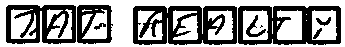
\includegraphics[height=1cm, width=5cm] {\filext{../bibliographie/image/biblio_manuscrit_maj}}\\
    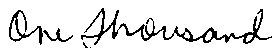
\includegraphics[height=1cm, width=5cm] {\filext{../bibliographie/image/biblio_manuscrit_man}}
    \end{array}$}$$
    \caption{Trois styles d'�criture, imprim�, b�ton, cursif.}
    \label{blibliographie_style_trois}
		\end{figure}
 
L'�criture imprim�e est un probl�me pour lequel les solutions existantes sont satisfaisantes. Elles commencent � �tre accessibles aux particuliers puisqu'elles accompagnent fr�quemment les logiciels fournis avec les scanners. Il existe par exemple des logiciels de lecture automatique de carte de visite. L'�criture b�ton concerne principalement les formulaires renseign�s manuellement comme les feuilles de maladie, les questionnaires � choix multiples. Contrairement � l'�criture imprim�e, l'objectif n'est pas de tout d�crypter mais au moins d'en traiter automatiquement une bonne partie avec un faible taux d'erreur tandis que les documents mal �crits seront toujours au soin d'un op�rateur de saisie. En revanche, les applications traitant la lecture de l'�criture manuscrite sont peu nombreuses. Il s'agit souvent de probl�mes pr�cis et r�duits comme la reconnaissance du montant litt�ral d'un ch�que, d'une date, quelques champs d'un formulaire. 

\indexfr{premi�re guerre mondiale}\indexfr{minist�re de la d�fense}\indexfr{raison du d�c�s}
Par exemple, le minist�re de la d�fense a r�cemment rendu publique une base de donn�es contenant les fiches de d�c�s de chaque soldat fran�ais durant la premi�re guerre mondiale\footnote{Voir le site \textit{http://www.memoiredeshommes.sga.defense.gouv.fr/} et l'article paru le 13 noveambre 2003 dans \emph{01 Informatique} num�ro 1745, page 12.}. Toutefois, la l�gislation fran�aise ne permet pas de publier un document contenant des informations d'ordre personnel, en particulier m�dical. Pourtant, le champ contenant la raison du d�c�s est susceptible de contenir ce genre d'information. Le probl�me consiste donc ici � d�terminer si ce champ contient une expression � caract�re m�dical mais sans avoir � la reconna�tre. Un traitement informatique a permis de r�pondre � cette question pour les deux tiers du million de documents avec 0,2\% d'erreur. 







\subsection{Probl�mes classiques de reconnaissance}

La reconnaissance de l'�criture hors ligne recouvre de nombreux probl�mes, des plus contraints, reconnaissance d'une lettre parmi une liste pr�d�finie, aux moins contraints, reconnaissance d'un paragraphe entier. Le probl�me de la figure~\ref{blibliographie_probleme} illustre la reconnaissance d'un pr�nom parmi une liste de choix possibles. Ce probl�me est pour le moment une r�f�rence car, pour l'�criture cursive, il est le moins contraint qu'on sache r�soudre avec des performances acceptables. Il est d�sign� plus simplement par l'expression \emph{reconnaissance avec dictionnaire}. \indexfr{dictionnaire}\indexfrr{reconnaissance}{dictionnaire}

		\begin{figure}[t]
    $$\frame{$\begin{array}[c]{c}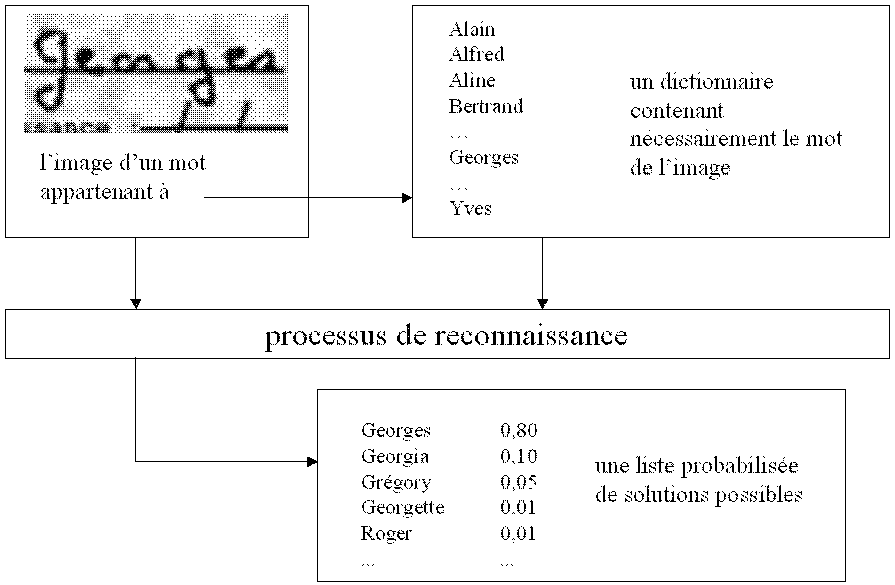
\includegraphics[height=6cm, width=10cm]
     {\filext{../bibliographie/image/probleme}}\end{array}$}$$
    \caption{Un probl�me classique de reconnaissance de l'�criture manuscrite~: 
    					reconnaissance avec dictionnaire\indexfr{dictionnaire}.}
    \label{blibliographie_probleme}
		\end{figure}


Le terme "acceptable" est volontairement flou, il d�pend beaucoup du probl�me. En ce qui concerne la reconnaissance d'un pr�nom parmi une liste en contenant environ~2000, pour 100~images, des performances acceptables correspondent � 69~images bien reconnues, 1~image mal reconnue et 30~images rejet�es car consid�r�es comme illisibles par le logiciel de reconnaissance. Ces performances sont acceptables parce qu'elles permettent � l'entreprise qui d�cide de recourir � ces m�thodes de r�duire le nombre de personnes affect�es � la saisie de ces informations, de r�duire ses co�ts de traitement.

\indexfr{productivit�}\indexfr{saisie}\indexfr{performances acceptables}

Par la suite, les algorithmes propos�s, bien qu'utilis�s pour l'�criture manuscrite cursive, pourront l'�tre pour les deux autres styles  mais seront vraisemblablement moins performants que des algorithmes sp�cifiquement d�velopp�s pour telle ou telle �criture. C'est encore plus vrai pour la reconnaissance en ligne qui utilise des informations suppl�mentaires relatives au d�placement du crayon.









\subsection{De l'image au r�sultat}
\label{biblio_image_resultat}


Le processus de reconnaissance part d'une image et aboutit � une liste de propositions accompagn�es d'une probabilit� (figure~\ref{blibliographie_probleme}). Ce long processus peut �tre d�coup� en trois parties illustr�es par la figure~\ref{blibliographie_systeme}~:

		\begin{enumerate}
		\item pr�traitement de l'image, 		\indexfr{pr�traitement de l'image}
		\item reconnaissance statistique, 	\indexfrr{reconnaissance}{statistique}
		\item d�cision. 										\indexfr{d�cision}
		\end{enumerate}

		\begin{figure}[ht]
    $$\begin{tabular}{|c|}\hline
   	\filefig{../bibliographie/fig_syswh}
    \\ \hline
    \end{tabular}
    $$
    \caption{		Sch�ma de l'ensemble du processus 
    						de reconnaissance d�coup� en trois parties~: pr�traitement de l'image,
                reconnaissance statistique, d�cision. La s�quence de graph�mes 
                est d�crite au paragraphe~\ref{image_segmentation_grapheme}.
                Le terme contexte regroupe toutes les informations inh�rentes au probl�me � r�soudre comme
                la langue, le type de document � traiter, le type d'information � reconna�tre (nom, pr�nom,
                montant, ...).}
    \label{blibliographie_systeme}
		\end{figure}

\indexfr{contexte}
La cha�ne des pr�traitements de l'image comprend essentiellement une segmentation en graph�mes (paragraphe~\ref{biblio_section_grapheme}), celle-ci consiste � scinder un probl�me complexe en plusieurs petits probl�mes plus simples. La reconnaissance statistique est centr�e autour d'un type de mod�le probabiliste adapt� � la s�quence de graph�mes obtenue � l'�tape pr�c�dente. Les mieux adapt�s sont les mod�les de Markov\seeannex{annexe_hmm_def}{mod�les de Markov cach�s} cach�s car ils associent s�quence et forme des graph�mes. Enfin, l'�tape de d�cision permet d'affiner les r�sultats de la reconnaissance statistique en associant plusieurs reconnaisseurs en tenant compte d'un contexe propre � l'exp�rience comme le code postal pour la lecture d'une adresse, ce qui permet d'avoir un a priori sur la ville � d�crypter. La reconnaisance statistique est fortement d�pendante de la langue\footnote{La langue dans laquelle les documents ont �t� �crits est une information importante ne serait-ce que de par le fait que les mots diff�rent d'une langue � l'autre, voire les lettres.} alors que les pr�traitements sont plut�t li�s au type de document exploit�, enveloppe, ch�ques, formulaires\footnote{Les traitements d'images sont plus d�pendants de la qualit� des documents (papier, scanner, ...), de leur structuration (formulaire, paragraphe, ...) que du contenu.}. 

Les trois couches du sch�ma~\ref{blibliographie_systeme} sont g�n�ralement ind�pendantes, ce sera le cas pour la majorit� des mod�les pr�sent�s au paragraphe~\ref{biblio_modelisation}. Le fait que ces trois �tapes s'encha�nent les unes � la suite des autres rend difficile la comparaison de chacune des parties qui composent le syst�me de reconnaissance. Il serait possible de comparer la partie statistique de deux syst�mes � partir du moment o� les deux autres parties (traitement d'image et d�cision) sont communes. Les articles publi�s pr�sentent rarement un syst�me dans sa globalit� et s'int�ressent � seulement une de ces trois parties qui sont plus rarement d�crites ensemble except� dans des th�ses ou des articles qui en sont issus (voir \citeindex{Senior1998}). \indexfrr{reconnaissance}{statistique} 
Une exception � cette r�gle pour l'article \citeindex{Verma2004}, ce dernier d�crit sommairement l'ensemble de son syst�me de reconnaissance afin de comparer les performances en reconnaissance de diff�rents types de caract�ristiques.





					\begin{figure}[t]
			    $$\begin{tabular}{|c|}\hline
			    \filefig{../bibliographie/fig_syswh2}
			    \\ \hline
			    \end{tabular} $$
			    \caption{		Sch�ma de l'ensemble du processus de reconnaissance d�coup� en trois parties principales~: 
			    						pr�traitement de l'image, description et reconnaissance statistique, d�cision. Les syst�mes de
			    						reconnaissance font de plus intervenir des traitements parall�les, divers reconnaisseurs,
			    						mis en comp�tition afin d'am�liorer le r�sultat final.}
			    \label{blibliographie_systeme_whole}
					\end{figure}

\indexfr{caract�ristiques}
\indexfr{reconnaissance}
\indexfr{d�cision}
\indexfr{description}

La figure~\ref{blibliographie_systeme_whole} illustre de mani�re exhaustive un tel syst�me. A partir de l'image, plusieurs pr�traitements sont possibles, plusieurs segmentations en graph�mes. Chacune d'elles peut � son tour �tre d�crite de mani�res diff�rentes par des caract�ristiques, qui sont � leur tour capables d'�tre reconnues par des mod�les vari�s. Les r�sultats sont regroup�s puis synth�tis�s pour aboutir � un seul r�sultat accompagn� d'un taux de confiance. M�me si cet ensemble est co�teux � �laborer et � apprendre, il semble que les syst�mes de reconnaissance bas�s sur un pr�traitement d'image, un jeu de caract�ristiques, un reconnaisseur aient atteint leur limite (voir \citeindex{Steinherz1999}, \citeindex{Vinciarelli2002} ou paragraphe~\ref{biblio_constat}).







\subsection{Annotation}\indexfr{annotation}

Par la suite, les termes \emph{annotation}, images \emph{annot�es} seront r�guli�rement employ�s. L'annotation d�signe une information qui accompagne chaque image, celle-ci est relative au contenu et renferme ce que les mod�les de reconnaissance devront apprendre. Par exemple, l'annotation la plus simple associ�e � une image du mot "GEORGES" est le mot "GEORGES" lui-m�me. Cette information peut �tre plus �tendue et inclure la description d'une segmentation en lettres. En r�gle g�n�rale, l'annotation est construite manuellement et devient la bonne r�ponse, celle que doit retourner le reconnaisseur s'il a bien appris. Tous les mod�les pr�sent�s dans ce document sont estim�s � partir d'une base d'images annot�es de mani�re � d�chiffrer correctement des images non annot�es. Selon les mod�les, l'annotation requise n'est pas la m�me. Plus l'annotation est fournie, plus la reconnaissance a de chances d'obtenir de bonnes performances. 





\subsection{Constat et limites}
\label{biblio_constat}
\indexfr{ch�que}
\indexfr{adresse postale}

L'article~\citeindex{Vinciarelli2002} brosse le portrait de la reconnaissance de l'�criture cursive et met en lumi�re les nombreuses �tapes r�sum�es dans le paragraphe~\ref{biblio_image_resultat} qui constituent un tel processus. Les recherches effectu�es dans les ann�es pr�c�dentes ont abouti aux mod�les de Markov cach�s qui sont encore � l'heure actuelle la mod�lisation la mieux adatapt�e. Leurs performances se sont d'ailleurs concr�tis�es par la commercialisation de produits offrant de bonnes performances mais dans des domaines pr�cis comme la reconnaissance du montant des ch�ques ou la lecture d'adresses postales. Ces deux aspects -~nombreuses �tapes, domaine pr�cis~- expliquent pourquoi il est difficile de comparer diff�rents syst�mes de reconnaissance. Il est donc impossible de choisir une mod�lisation plut�t qu'une autre lorsqu'elles n'utilisent pas les m�mes pr�traitements. La reconnaissance est aussi am�lior�e par le contexte de l'exp�rience qui nuit en m�me temps � une comparaison fiable de deux syst�mes puisqu'ils sont utilis�s dans des conditions d'exp�rience diff�rentes. Dans le cas des ch�ques, montants litt�ral et num�rique sont mis en correspondances, dans le cas d'une adresse, c'est le cas pour la ville et le code postal.

La reconnaissance de l'�criture manuscrite a donc beaucoup suscit� l'int�r�t des chercheurs dans les ann�es 1990 � 2000. Les diff�rentes solutions propos�es ont difficilement pu �tre compar�es puisque apprises sur des donn�es rarement identiques dans des contextes rarement semblables. Elles proposent malgr� tout des solutions exploitables industriellement qui permettent d'envisager la reconnaissance d'un mot manuscrit dans un vocabulaire r�duit comme un probl�me quasiment r�solu. Toutefois, ces m�mes mod�les ont montr� leur limite appliqu�s � des probl�mes moins contraints, o� le contexte est moins important. L'article~\citeindex{Steinherz1999} sugg�re d'ailleurs que la recherche soit plut�t dirig�e vers l'am�lioration de la d�cision plut�t que la reconnaissance elle-m�me.

Ce chapitre d�crira sommairement les deux premi�res parties d'un syst�me de reconnaissance, abord�es de mani�re plus d�taill�e dans les deux chapitres suivants.







%------------------------------------------------------------------------------------------------------------
\section{Les pr�traitements d'image} \indexfr{pr�traitement de l'image}
%-------------------------------------------------------------------------------------------------------------


Les articles relatifs � cette partie sont moins nombreux. Les algorithmes utilis�s sont plus le r�sultat d'exp�riences, d'une succession d'heuristiques, plut�t que le corollaire d'une mod�lisation th�orique de l'image. L'article \citeindex{Simon1992} s'int�resse � une segmentation d'un mot � partir du squelette de l'image (voir �galement \citeindex{Lecolinet1990}). Le r�sultat souhait� est une segmentation proche des caract�res (\citeindex{Lecolinet1996}).

Le r�sultat peut �tre simple et aboutit � des morceaux de petites tailles qui sont plus difficiles � traiter par la suite lors de la reconnaissance statistique. La m�thode des fen�tres glissantes (voir~\citeindex{Knerr2001}, figure~\ref{blibliographie_window_slide}) fait partie de cette cat�gorie.\indexfrr{fen�tre}{glissante} L'image d'un mot est simplement d�coup�e en bandelettes verticales sans relation avec les lettres. La reconnaissance est d�volue � des mod�les math�matiques complexes.

Le r�sultat peut �tre plus travaill� et inclure les r�sultats de nombreuses exp�riences sous forme d'heuristiques. La segmentation obtenue est plus proche de celle des lettres et plus instable aussi car ce traitement est un assemblage de r�gles essaim�es lors de squelettisations, de nettoyages ou de segmentations.\indexfr{squelettisation}\indexfr{nettoyage}\indexfr{segmentation} En contre partie, les mod�les de reconnaissance statistique peuvent se limiter � la reconnaissance de caract�res m�me s'il n'est pas encore possible � ce stade de segmenter en lettres de mani�re parfaite � moins de savoir d�j� reconna�tre ce qu'est une lettre. Par exemple, d'autres travaux (\citeindex{Knerr2000}) explorent la possibilit� de reconstituer l'information temporelle relative au trac�\indexfr{trac�} pr�sente en reconnaissance en ligne\indexfr{en ligne} � partir de l'image �crite. Le syst�me apprend cette t�che � partir d'une base d'images coupl�es avec une autre base contenant les d�placements du stylo. La segmentation est conclue par la construction d'une s�quence ou d'un graphe de petites images appel�es
\emph{graph�mes}.\indexfr{graph�me}


    \begin{figure}[ht]
    $$\frame{$\begin{array}[c]{c}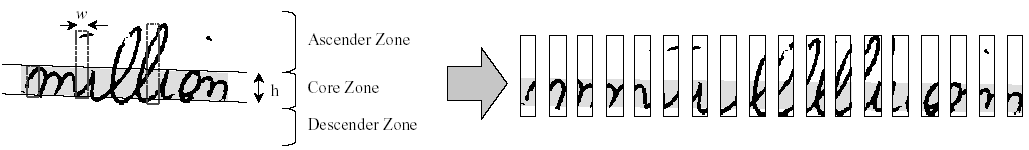
\includegraphics[height=2cm, width=16cm]
     {\filext{../bibliographie/image/biblio_window_slide}}\end{array}$}$$
    \caption{Image extraite de~\citeindexfig{Knerr2001} illustrant le d�coupage 
    					de l'image d'un mot par des fen�tres glissantes.}
    \label{blibliographie_window_slide}
    \end{figure}








\subsection{Graph�mes}
\label{biblio_section_grapheme}


Le sens de lecture de gauche � droite apparente la reconnaissance de l'�criture � la reconnaissance de la parole. L'analogie n'est valable que si l'image en deux dimensions d'un paragraphe \indexfr{paragraphe} (figure~\ref{blibliographie_paragraphe}) est d�compos�e d'abord en lignes \indexfrr{segmentation}{ligne} (figure~\ref{blibliographie_paragraphe_ligne}) puis en caract�res ou demi-caract�res de mani�re � retrouver cet ordonnancement de gauche � droite comparable au d�coupage temporel inh�rent � la reconnaissance vocale (voir figure~\ref{blibliographie_paragraphe_car}). \indexfr{caract�re}

Plut�t que d'utiliser des fen�tres glissantes, \indexfrr{fen�tre}{glissante} les premi�res segmentations
�labor�es ont tout de suite cherch� � isoler les lettres. Ce r�sultat difficile � obtenir r�duit par la suite la taille des mod�les de reconnaissance des caract�res alors que les fen�tres glissantes aboutissent � des images de caract�res d�cor�es de bouts de caract�res voisins qui s'apparentent � du bruit. Cette plus grande variabilit� m�ne � des mod�les de reconnaissance plus consistants. Cette diff�rence n'est plus importante aujourd'hui mais l'�tait il y a dix ans lorsque les ordinateurs �taient limit�s en m�moire.

		\begin{figure}[ht]
    $$\frame{$\begin{array}[c]{c}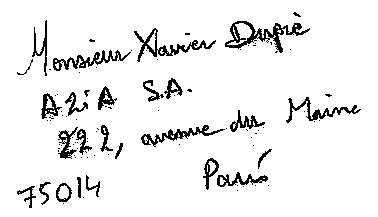
\includegraphics[height=3cm, width=5cm]
     {\filext{../bibliographie/image/biblio_paragraphe}}\end{array}$}$$
    \caption{Image d'un paragraphe manuscrit.}
    \label{blibliographie_paragraphe}
		\end{figure}

		\begin{figure}[ht]
    %$$\frame{$\begin{array}[c]{c}\includegraphics[height=4cm, width=6cm]
    %{../bibliographie/image/biblio_paragraphe_ligne}}\end{array}$}$$
    $$\frame{$\begin{array}[c]{c}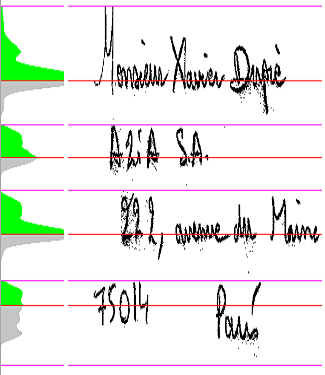
\includegraphics[height=4cm, width=6cm]
    {\filext{../bibliographie/image/biblio_histog}}\end{array}$}$$
    \caption{	Image des lignes d'un paragraphe figure~\ref{blibliographie_paragraphe} segment�es 
    					� partir d'histogramme (partie gauche de l'image). \indexfr{histogramme}}
    \label{blibliographie_paragraphe_ligne}
		\end{figure}

		\begin{figure}[ht]
    $$\frame{$\begin{array}[c]{c}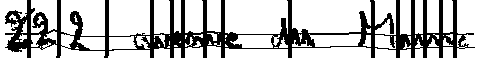
\includegraphics[height=0.8cm, width=6cm]
    {\filext{../bibliographie/image/biblio_paragraphe_car}}\end{array}$}$$
    \caption{	Graph�mes de la troisi�me ligne de la figure~\ref{blibliographie_paragraphe_ligne}. 
    					\indexfr{graph�me}}
    \label{blibliographie_paragraphe_car}
		\end{figure}

\indexfrr{segmentation}{ligne}\indexfrr{segmentation}{mot}

Les segmentations en lignes et en mots peuvent �tre r�alis�es � partir d'histogrammes (figure~\ref{blibliographie_paragraphe_ligne}) \indexfr{histogramme} sommant les pixels noirs de l'image dans
une direction parall�le � celle de segmentation. Les pics et les creux de l'histogramme permettent de d�terminer sans trop d'erreurs le bon d�coupage. Comme les histogrammes obtenus sont liss�s avant leur exploitation, les r�sultats sont assez stables � moins que l'image ne contienne des traits parall�les � la direction de segmentation comme un mot soulign�. C'est pourquoi l'image est d'abord nettoy�e, \indexfr{nettoyage} d�barrass�e de pixels isol�s et des grands traits horizontaux ou verticaux susceptibles de n'appartenir � aucune lettre. Ce nettoyage est g�n�ralement fait � partir d'une squelettisation. \indexfr{squelettisation}

Malheureusement, cette m�thode simple n'est pas applicable � une segmentation en caract�res. Comme le montre la
figure~\ref{blibliographie_window_slide}, les lettres sont souvent pench�es et se pr�tent mal � un d�coupage vertical.


\indexfrr{graph�me}{stabilit�}

Les graph�mes repr�sentent donc une meilleure segmentation puisqu'elle est plus proche des caract�res, elle est aussi plus sensible au bruit car elle est parfois bas�e sur une squelettisation comme l'illustre la figure~\ref{blibliographie_grapheme_2} (voir~\citeindex{Lecolinet1990}, \citeindex{Simon1992}). Le squelette est une image plus facile � traiter car il peut �tre repr�sent� sous forme de graphe. Le d�coupage est effectu� en rep�rant les ascendants et les descendants sur le squelette, \indexfr{squelettisation} toute forme en "u" est suppos�e �tre la fronti�re entre deux lettres. Par la suite, les r�gles sont affin�es par de nombreuses exp�riences. Ce pr�traitement aboutit � une s�quence de petites images appel�es \emph{graph�mes}\indexfr{graph�me} (figures~\ref{blibliographie_grapheme}, \ref{blibliographie_grapheme_2}) qu'il faut d�crire d'une mani�re exploitable par des mod�les math�matiques de reconnaissance tels que des r�seaux de neurones.



		\begin{figure}[t]
    $$\frame{$\begin{array}[c]{c}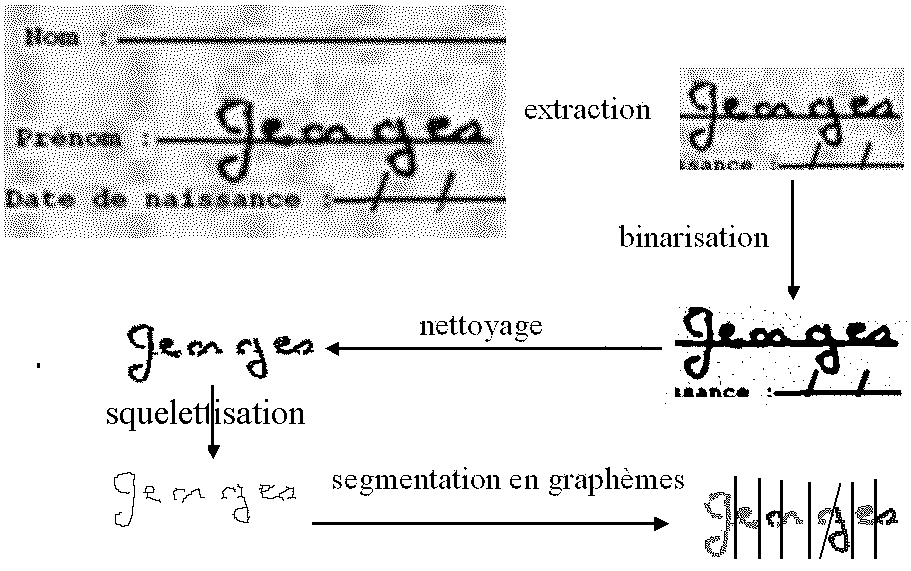
\includegraphics[height=6cm, width=10cm]
     {\filext{../bibliographie/image/pretraitement_image}}\end{array}$}$$
    \caption{De l'image � la segmentation en graph�mes, \indexfr{graph�me} le mot est extrait, 
    					son image est binaris�e, puis nettoy�e
             des bruits r�siduels et enfin segment�e en graph�mes souvent en utilisant le squelette. 
             Les nettoyages sont parfois adapt�s de mani�re sp�ficique � un type de
             document pr�cis. Ici, le pr�nom d�borde souvent sur l'intitul� \textit{Date de naissance}, 
             les nettoyages sont donc faits en cons�quence.}
    \label{blibliographie_grapheme}
		\end{figure}


		\begin{figure}[ht]
    $$\frame{$\begin{array}[c]{c}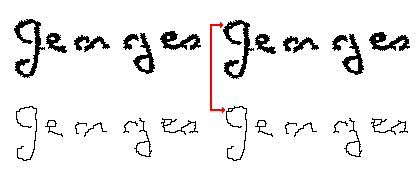
\includegraphics[height=3cm, width=6cm]
    {\filext{../bibliographie/image/biblio_graph_hole}}\end{array}$}$$
		\caption{	Stabilit� de la squelettisation, deux images du m�me mot dont la seule diff�rence 
              r�side dans deux pixels manquant
              dans le second exemple. Le squelette s'en trouve modifi� et la segmentation du premier 
              "g" passe de un graph�me � deux.}
			\indexfr{graph�me}
			\indexfrr{graph�me}{stabilit�}
			\indexfr{squelettisation}    
			\label{blibliographie_grapheme_2}
		\end{figure}


Ce pr�traitement est constitu� d'heuristiques qui le rendent instable et qui sont adapt�es au probl�me de
reconnaissance � r�soudre, par exemple, la segmentation de chiffres imprim�s \indexfrr{style}{imprim�} est diff�rente de celle de chiffres cursifs qui peuvent �tre attach�s. \indexfrr{style}{cursif} \indexfr{segmentation}

Pourquoi d�couper~? Pourquoi ne pas conserver l'image du mot dans son int�gralit� plut�t que de la segmenter avec une m�thode instable~? Deux arguments penchent pourtant en sa faveur~:

    \begin{enumerate}
    \item Il est plus facile de d�crire des morceaux de lettres plut�t que l'image compl�te du mot.
    \item Dans un probl�me o� les mots sont peu nombreux, il est facile de classer telle ou telle 
    			image comme �tant tel ou tel mot. Lorsque ce nombre de mots est grand 
    			(quelques milliers), la classification devient impossible. 
          Il est pr�f�rable de classer des objets plus petits comme les lettres ou des morceaux de lettres.
    \end{enumerate}

Un exemple de segmentation sera repris en d�tail au paragraphe~\ref{image_choix_segmentation}. Un r�sultat parfait est difficile � obtenir quelle que soit la m�thode si aucune reconnaissance n'est associ�e � cette segmentation. 




\subsection{Segmention explicite-implicite}
\indexfrr{segmentation}{explicite}
\indexfrr{segmentation}{implicite}


La litterature (voir~\citeindex{Vinciarelli2002}) distingue parfois deux types de segmentations~: implicite et explicite. Lorsque la segmentation en graph�mes a pour objectif le d�coupage de l'image d'un mot directement en lettres, celle-ci est explicite. La reconnaissance de ce mot est alors r�duite � une reconnaissance de caract�res. En revanche, lorsque la segmentation en graph�mes d�coupe cette image en lettres ou en morceaux de lettres, la reconnaissance statistique doit int�grer le fait qu'une lettre est constitu�e d'un ou plusieurs morceaux. Par cons�quent, la segmentation est dite implicite car les lettres n'apparaissent jamais de mani�re explicite.

\indexfrr{segmentation}{paradoxe de Sayre}
\indexfr{paradoxe de Sayre}
\indexfr{sur-segmentation}
L'article~\citeindex{Sayre1973} souligne le paradoxe de la segmentation implicite qui se r�sume par cette phrase~: une lettre ne peut �tre segment�e avant d'avoir �t� reconnue et ne peut �tre reconnue avant d'avoir �t� segment�e. Par cons�quent, les segmentations explicites sont plut�t un compromis, pas assez pr�cises pour d�finir explicitement des lettres, mais suffisamment pour avoir une association graph�me-lettre relativement simple. En r�gle g�n�rale, elles tentent de segmenter l'image d'un mot en morceaux qui sont inclus dans le dessin d'une lettre. Ces segmentations sont souvent regroup�es sous le terme \emph{sur-segmentation}.










\subsection{Caract�ristiques}
\label{biblio_caracteristique}


Etant donn� que les graph�mes \indexfr{graph�me} peuvent avoir des tailles variables, l'�tape suivante consiste
� d�crire ces images par un vecteur de caract�ristiques de dimension fixe. \indexfr{caract�ristiques} Ces
nombres sont r�els et chacun d'eux est cens� d�crire un aspect de l'image comme~:

    \begin{description}
    \itemm la taille du graph�me (largeur, hauteur),
    \itemm l'aire occup�e par les pixels noirs,
    \itemm le barycentre des pixels noirs,
    \itemm l'inclinaison,
    \itemm l'�paisseur moyenne des traits vetircaux et horizontaux, 
    				ces chiffres peuvent �tre calcul�s sur l'image enti�re ou une des
            bandes verticales ou horizontales, l'image est d�coup�e en quatre ou cinq, selon la r�solution,
    \itemm le nombre moyen de traits verticaux et horizontaux (transition pixel noir - 
    				pixel blanc sur une colonne de l'image),
    \itemm la position relative du pr�c�dent graph�me, du suivant.
    \end{description}

Ce n'est qu'une description parmi les nombreuses possibles dont un �ventail est propos� au paragraphe~\ref{reco_description_grapheme}. En d�finitive, ce pr�traitement transforme l'image d'un mot en une s�quence de vecteurs de dimension fixe ou \emph{mot math�matique}. Si cette dimension est not�e $D$, un mot math�matique est donc : 

\indexfr{mot}\indexfr{s�quence}

			\begin{xdefinition}{mot math�matique}
			\label{biblio_definition_mot_statistique}%
			\indexfrr{mot}{math�matique}%
			On d�finit un mot math�matique comme une s�quence finie de vecteurs de dimension fixe~:
			    $$
			    \text{mot} \longleftrightarrow m \in \pa{\R^D}^\N
			    $$
			o� $D$ est la dimension de l'espace des caract�ristiques. \indexfr{caract�ristiques}
			\end{xdefinition}


\indexfrr{dimension}{infinie}
Le passage d'une s�quence d'images � une s�quence de vecteurs sera d�crit en d�tail au paragraphe~\ref{reco_description_grapheme}. La reconnaissance est similaire � un probl�me de classification. Cette t�che est un probl�me classique lorsqu'il s'agit d'un espace vectoriel de dimension finie. En revanche, la classification dans l'espace des mots math�matiques (de dimension infinie) est une t�che plus ardue que le paragraphe~\ref{biblio_reconnaissance_statistique} et pour laquelle le paragraphe~\ref{biblio_modelisation} recense des solutions existantes.








%-----------------------------------------------------------------------------------------------------------------
\section{Reconnaissance statistique}
%-----------------------------------------------------------------------------------------------------------------
\label{biblio_reconnaissance_statistique}


\subsection{Classification en mots} \label{section_classification_mots}

\indexfrr{classification}{mot} 
\indexfrr{reconnaissance}{dictionnaire} 
\indexfrr{mot}{math�matique} 

Dans le cas du probl�me de reconnaissance avec dictionnaire, reconna�tre un mot �crit sur une image revient �
classer le mot math�matique qui lui correspond dans la classe qui regroupe toutes les �critures diff�rentes de ce m�me mot (figure~\ref{blibliographie_same_word}). La reconnaissance est un probl�me de classification.

\indexfr{classification} 
\indexfr{reconnaissance} 
\indexfrr{mot}{math�matique} 
\indexfr{�tiquette}%

		\begin{figure}[ht]
    $$\frame{$\begin{array}[c]{ccc}
    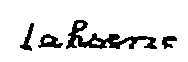
\includegraphics[height=0.75cm,     width=3cm] {\filext{../bibliographie/image/biblio_cursif_exemple_1}} &
        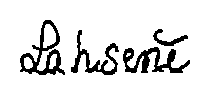
\includegraphics[height=0.75cm, width=3cm] {\filext{../bibliographie/image/biblio_cursif_exemple_2}} &
        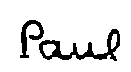
\includegraphics[height=0.75cm, width=2cm] {\filext{../bibliographie/image/biblio_cursif_exemple_3}} \\
    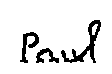
\includegraphics[height=0.75cm,     width=2cm] {\filext{../bibliographie/image/biblio_cursif_exemple_4}} &
        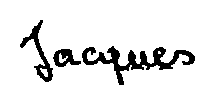
\includegraphics[height=0.75cm, width=3cm] {\filext{../bibliographie/image/biblio_cursif_exemple_5}} &
        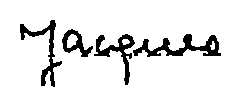
\includegraphics[height=0.75cm, width=3cm] {\filext{../bibliographie/image/biblio_cursif_exemple_6}} \\
    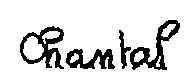
\includegraphics[height=0.75cm,     width=2cm] {\filext{../bibliographie/image/biblio_cursif_exemple_10}} &
        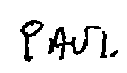
\includegraphics[height=0.75cm, width=2cm] {\filext{../bibliographie/image/biblio_cursif_exemple_8}} &
        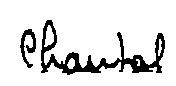
\includegraphics[height=0.75cm, width=3cm] {\filext{../bibliographie/image/biblio_cursif_exemple_9}} 
    %& 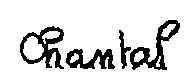
\includegraphics[height=0.75cm,   width=3cm] {\filext{../bibliographie/image/biblio_cursif_exemple_10}} &
    \end{array}$}$$
    \caption{Plusieurs mani�res d'�crire le m�me mot.}
    \label{blibliographie_same_word}
		\end{figure}


Pour chaque classe de mots, un mod�le math�matique est construit afin de mod�liser l'ensemble des mots math�matiques
lui correspondant. Ensuite, pour attribuer la bonne classe � un mot math�matique, tous les mod�les de mots sont
sollicit�s et celui qui donne la meilleure r�ponse est consid�r� comme la bonne r�ponse
(figure~\ref{blibliographie_reponse_modele}).

		\begin{figure}[ht]
    $$\frame{$\begin{array}[c]{c}
    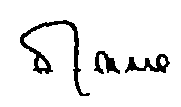
\includegraphics[height=1.5cm, width=3cm]
    	 {\filext{../bibliographie/image/biblio_cursif_ex_reco}} \\
        \begin{array}{lllll}
        MARIO   &   0,782 & & MARIA   &   0,004 \\
        MAIRE   &   0,108 & & FRANC   &   0,002 \\
        MARIE   &   0,076 & & FRANS   &   0,002 \\
        MAUD    &   0,023 & & HANS    &   0,001 \\
        ...     &   ...   & & ...     &   ...
        \end{array}
    \end{array}$}$$
    \caption{R�ponse des mod�les math�matiques associ�s aux mots du dictionnaire.}
    \label{blibliographie_reponse_modele}
		\end{figure}


L'avantage majeur de cette organisation est le possible ajout de mod�les. Par exemple, en ce qui concerne la reconnaissance du montant litt�ral des ch�ques, le passage � l'euro consiste � ajouter le mot \emph{EURO} \indexfr{euro} � l'ensemble des mots possibles pour �crire un montant. 

\indexfrr{mod�le}{mot}\indexfrr{mod�le}{lettre} 

La construction des mod�les de mots d�pend du probl�me � r�soudre. Toujours dans le cas de la reconnaissance avec dictionnaire, \indexfrr{reconnaissance}{dictionnaire} si le dictionnaire est petit (pas plus d'une centaine de mots), un mod�le par mot sera construit, c'est-�-dire qu'il aura �t� appris pour reconna�tre ce mot. Dans le cas d'un grand dictionnaire (quelques millieurs de mots), on pr�f�rera obtenir ce mod�le de mot par l'assemblage de mod�les de lettres, qui auront appris � reconna�tre sp�cifiquement les lettres. C'est dans cette optique qu'une bonne segmentation en graph�mes \indexfr{graph�me} est importante. Si un graph�me repr�sente plus d'une lettre, la reconnaissance aura toutes les chances d'�tre fauss�e.






\subsection{S�quence et forme} 

\indexfr{s�quence} \indexfr{forme} \indexfr{mot} \indexfr{mod�le} \label{section_classification_lettre} 


La d�finition~\ref{biblio_definition_mot_statistique} d�finit un mot math�matique comme une s�quence de vecteurs, ceci signifie qu'� un mot correspond des mots math�matiques de longueurs diff�rentes et de vecteurs diff�rents mais de dimension fixe. Le paragraphe~\ref{biblio_section_grapheme} a d�j� r�pondu � propos de l'int�r�t de conserver un param�tre variable dans la description de l'image d'un mot. Cette description fait donc intervenir deux aspects~:

    \begin{enumerate}
    \item une \emph{s�quence} de longueur variable,
    \item la \emph{forme} des graph�mes car cette s�quence est 
    				compos�e de vecteurs de dimension fixe d�crivant la \emph{forme}
            de chacun des graph�mes qui la composent.  \indexfr{graph�me}
    \end{enumerate}



\label{biblio_grapheme_segmentation_choix}

Dans les mod�les pr�sent�s dans ce document, beaucoup traitent ces deux aspects s�par�ment. La forme, le plus simple des deux aspects puisque de dimension fixe, est trait�e par un classifieur \indexfr{classifieur} qui peut �tre un r�seau de neurones, \indexfr{RN} une machine � support vectoriel plus connu sous sa d�nomination anglaise \emph{Support Vector Machine} (SVM), \indexfr{SVM} un arbre de d�cision... 

La s�quence est principalement mod�lis�e par des mod�les de Markov cach�s. \indexfr{MMC} Ceux-ci ont �t� d�velopp�s par Baum (\citeindex{Baum1968}, \citeindex{Baum1972}) et s'inscrivent dans un probl�me plus g�n�ral d�crit par Dempster (\citeindex{Dempster1977}) qui expose pour la premi�re fois l'algorithme EM (expectation-maximisation),\indexfr{EM}\indexsee{expectation}{EM}\indexfr{maximisation} permettant d'estimer les param�tres d'un mod�le prenant en compte des observations cach�es. Les mod�les de Markov cach�s en sont un cas particulier. Pour terminer la liste des articles cit�s chaque fois, il faut mentionner une excellente introduction (\citeindex{Rabiner1986}) dont l'�tude est approfondie par~\citeindex{Levinson1983}. Toutefois, ces articles ne pr�sentent que des cha�nes de Markov cach�es discr�tes qu'il faut adapter afin qu'elles prennent en compte l'aspect forme qui, lui, est continu. Un mod�le int�grant le couple s�quence-forme de mani�re s�par�e constitue un mod�le appel� \emph{hybride} ou
\emph{semi-continu}. 

\indexfr{hybride} \indexfr{semi-continu}
















\subsection{Choix d'une mod�lisation}

Choisir une mod�lisation math�matique pour un probl�me impose de faire certaines hypoth�ses sur les donn�es � repr�senter (ind�pendance temporelle, la loi probabiliste qu'elles suivent,~...). Une fois celles-ci converties en un mod�le, il peut contenir plus ou moins de degr�s de libert�. Plus il en a, plus il peut s'adapter facilement aux donn�es � mod�liser et plus il s'adapte difficilement � de nouvelles donn�es. 

Les hypoth�ses doivent donc �tre les mieux adapt�es, elles conditionnent la structure du mod�le (mod�les de Markov cach�s, r�seaux de neurones, ...).   \indexfr{mod�lisation}\indexfr{hypoth�se} Il suffit de d�terminer le choix du degr� de libert� (ou nombre de coefficients) pour le mod�le s�lectionn�. \indexfr{degr� de libert�} Le choix des hypoth�ses est toujours le plus important car il d�termine les algorithmes d'estimation des param�tres et ceux de leur utilisation. Diverses mod�lisations sont pr�sent�es par la suite.











%------------------------------------------------------------------------------------------------------------------
\section{Mod�lisation}
%------------------------------------------------------------------------------------------------------------------
\label{biblio_modelisation}








\subsection{Mod�les de Markov cach�s hybrides et classifieur quelconque}

\label{biblio_mmc_classifieur} 
\indexfrr{MMC}{+classifieur} \indexfr{classifieur}
\indexfr{s�quence} \indexfr{caract�ristiques}
\indexfrr{�criture}{arabe}

Cette mod�lisation est utilis�e depuis quelques ann�es pour la reconnaissance de textes en �criture romaine et est plus r�cemment adapt�e pour la reconnaissance de textes arabes (\citeindex{Khorsheed2003}). C'est le mod�le le plus simple, � chaque vecteur de caract�ristiques est associ�e une classe de mani�re � transformer la s�quence de vecteurs d'observations continues en s�quence d'observations discr�tes (figure~\ref{blibliographie_mmc_classifieur}). Ce mod�le convertit ensuite cette s�quence en une probabilit�~: celle que le mod�le �mette cette s�quence discr�te. Ce processus est r�p�t� pour chaque mod�le de mot, le mot reconnu est celui ayant obtenu la meilleure probabilit� d'�mission\seeannex{interdoc_mmc}{MMC}. \indexfrr{probabilit�}{�mission}

		\begin{figure}[ht]
    $$\frame{$\begin{array}[c]{c}
    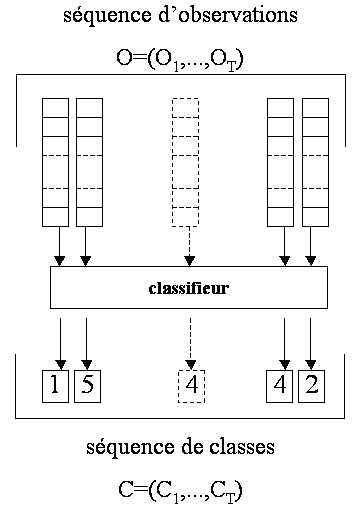
\includegraphics[height=6cm, width=5cm] {\filext{../bibliographie/image/biblio_mmc_classifieur}} \\
    \end{array}$}$$
    \caption{Mod�le de Markov cach� + classifieur.}
    \label{blibliographie_mmc_classifieur}
		\end{figure}

Les classifieurs peuvent �tre de toutes sortes (s�parateurs lin�aires, centres mobiles, r�seau de neurones, r�seau de Kohonen, arbre de d�cision, SVM...).\indexfr{lin�aire}\indexfr{RN}\indexfr{Kohonen}\indexfr{centres mobiles}\indexfr{SVM}\indexfrr{arbre}{d�cision} Le choix de ces mod�les est influenc� par le fait que les observations sont annot�es (leur classe est connue) ou non. \indexfr{annotation} Si elles sont annot�es, les graph�mes sont de taille suffisante \indexfr{graph�me} pour �tre interpr�t�s (lettres ou parties de lettres), dans ce cas, cette interpr�tation ou classification donn�e est alors apprise par le classifieur\footnote{Cette annotation est en g�n�ral co�teuse � obtenir puisqu'il faut segmenter manuellement chaque image puis classer chaque morceau ou lettre.}. Cette m�thode poss�de l'avantage de fixer le nombre de classes mais aussi l'inconv�nient de parfois g�n�rer des ambigu�t�s car certaines diff�rences apparaissant sur l'image peuvent dispara�tre dans le vecteur de caract�ristiques. De plus, au niveau de l'image, la lettre "u" divis�e en deux parties ressemble fortement � deux lettres "i". Si elles ne sont pas annot�es, la classification est automatique (centres mobiles par exemple) mais il reste � d�terminer le nombre de classes id�al. Cette partie peut faire l'objet d'une �tude statistique pr�alable\seeannex{classification_non_supervisee}{classification non supervis�e}. 
    

Soit un mot math�matique not� $O = \vecteur{O_1}{O_T}$ et la s�quence des classes d'observations associ�e � ce mot $C = \vecteur{C_1}{C_T}$ (annotation), \indexfr{annotation} on d�finit la probabilit� que le mod�le $M$ �mette la s�quence $O$ par~: \indexfrr{probabilit�}{�mission}

			\begin{eqnarray}
			\pr{O \sachant M}  &=&     \summyone{\vecteur{q_1}{q_T}}   \pr{O,\vecteurno{q_1}{q_T} \sachant M} \nonumber \\
			                   &=&     \summyone{\vecteur{q_1}{q_T}}   \cro{\pr{q_1 \sachant M} \pr{C_1 \sachant q_1, M}
			                           \prody{t=2}{T} \pr{q_t \sachant q_{t-1}, M} \pr{C_t \sachant q_t,M}}
			                           \label{biblio_equation_hmm} \\
			 && \text{o� } \vecteur{q_1}{q_T} \text{ est une s�quence d'�tats du mod�le} \nonumber
			\end{eqnarray}

L'�quation (\ref{biblio_equation_hmm}) d�coule des hypoth�ses inh�rentes aux cha�nes de Markov cach�es d'ordre~un\seeannex{interdoc_mmc}{cha�ne de Markov cach�e}. Cette mod�lisation fait intervenir deux d�cisions~:%

    \begin{enumerate}
    \item La premi�re est prise par le classifieur qui attribue une classe � chaque graph�me.
    				\indexfr{graph�me}
    \item La seconde est prise par le module de d�cision qui d�cide de lire dans l'image le mot dont 
    				le mod�le associ�
            est le plus probable.
    \end{enumerate}

La seconde d�cision est incontournable mais la premi�re peut l'�tre en adoptant une mod�lisation plus fine comme celle des paragraphes~\ref{biblio_mmc_gauss} et~\ref{biblio_mmc_rn}.



Ces mod�les sont utilis�s par \citeindex{Knerr2001} qui compare leurs r�sultats � ceux de mod�les de Markov cach�s discrets. L'int�r�t de cet article porte sur l'utilisation de leurs propri�t�s lors de la segmentation d'une image d'un mot en lettres (figure~\ref{blibliographie_knerr_2001}). Plusieurs topologies de cha�nes de Markov sont expos�es accompagn�es de l'id�e qui a pr�sid� � leur �laboration. Ces mod�les sont aussi utilis�s dans la th�se \citeindex{Augustin2001} qui aborde le probl�me de la recherche de la meilleure topologie de la cha�ne de Markov (paragraphe~\ref{biblio_architecture}). Ces mod�les font encore l'objet de recherche, \citeindex{Koerich2002b} pr�sente leur utilisation pour de grands vocabulaires.



		\begin{figure}[t]
    $$\frame{$\begin{array}[c]{c}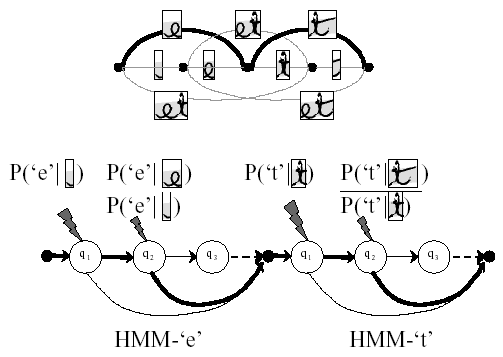
\includegraphics[height=6cm, width=9cm]
    {\filext{../bibliographie/image/biblio_knerr_2001}}\end{array}$}$$
    \caption{Image extraite de~\citeindexfig{Knerr2001}, elle repr�sente un graphe de segmentation du mot "et", 
    								parmi toutes les
                    possibilit�s, celle en trait gras est la plus probable.}
    \label{blibliographie_knerr_2001}
		\end{figure}













\subsection{Mod�les de Markov cach�s hybrides et lois gaussiennes}%

\label{biblio_mmc_gauss} \indexfrr{MMC}{+Gauss} \indexfrr{loi}{gaussienne} \indexfrr{loi}{normale}
\indexfrr{loi}{normale multidimensionnelle}%

Au lieu de classer les observations afin de les rendre discr�tes, celles-ci sont suppos�es suivre une loi normale, diff�rente pour chaque �tat du mod�le (\citeindex{Bottou1991}), ou �tre partag�es par plusieurs �tats � la fois (\citeindex{Bunke1995}). L'expression de la probabilit� d'�mission est r�sum�e par les deux �quations (\ref{biblio_equation_gauss}) et (\ref{biblio_equation_gauss_emission})~:



    \begin{eqnarray}
    \pr{O \sachant M}  &=&     \summyone{\vecteur{q_1}{q_T}}   \cro{\pr{q_1 \sachant M} \pr{O_1 \sachant q_1, M}
                                                                \prody{t=2}{T} \pr{q_t \sachant q_{t-1}, M} 
                                                                \pr{O_t \sachant q_t,M}}
                                                                \label{biblio_equation_gauss} \\
    && \text{o� } \pr{O_t \sachant q_t=i, M} =  \dfrac{1}{\pa{2\pi}^{\frac{n}{2}} \sqrt{ \det \pa{ V_i}} }
                            \; e ^{\pa{ - \frac{1}{2} \pa{O_t - \mu_i}' \,  \pa{V_i}^{-1} \pa{O_t - \mu_i}}}
                            \label{biblio_equation_gauss_emission} \\
    && \text{avec } n \text{ la dimension de l'espace vectoriel des observations} \nonumber 
		\end{eqnarray}


L'inconv�nient de ce mod�le est sa gourmandise : pour des vecteurs d'observations de 50 caract�ristiques, la matrice carr�e $V_i$ contient 2500 coefficients et ce pour chaque �tat de la cha�ne de Markov. Par cons�quent, l'utilisation de ces mod�les s'accompagne d'hypoth�ses simplificatrices : $V_i$ est souvent suppos�e diagonale.









\subsection{Mod�les de Markov cach�s hybrides et r�seau de neurones}%
\label{para_biblio_image_reco}

\label{biblio_mmc_rn} \indexfrr{MMC}{+RN} \indexsee{r�seau de neurones}{RN} \indexfr{RN} \indexsee{neural network}{RN}
\indexsee{NN}{RN}


Le classifieur de la figure~\ref{blibliographie_mmc_classifieur} est remplac� par un r�seau de neurones illustr� par la figure~\ref{blibliographie_mmc_rn}. Il associe � une s�quence d'observations $O = \vecteur{O_1}{O_T}$ une s�quence de vecteurs de probabilit�s $V = \vecteur{V_1}{V_T}$ o� $V_t = \vecteur{V_t^1}{V_t^L}$ et $\summy{k=1}{L} V_t^k = 1$. L'expression\seeannex{definition_mmc_1}{MMC} de la probabilit� devient~:

		\begin{figure}[t]
    $$\frame{$\begin{array}[c]{c}
    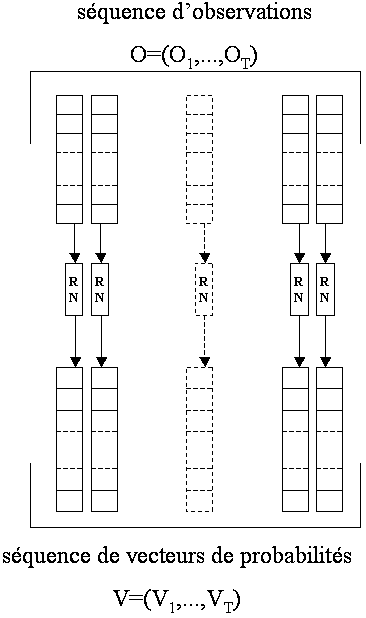
\includegraphics[height=7cm, width=5cm] 
    {\filext{../bibliographie/image/biblio_mmc_rn}} \\
    \end{array}$}$$
    \caption{Mod�le de Markov cach� + r�seau de neurones}
    \label{blibliographie_mmc_rn}
		\end{figure}

			\begin{eqnarray}
			\pr{O \sachant M}  &=&     \summyone{\vecteur{q_1}{q_T}}   \pr{O,\vecteurno{q_1}{q_T} \sachant M} \nonumber \\
			\pr{O \sachant M}  &=&     \summyone{\vecteur{q_1}{q_T}}   \cro{\pr{q_1 \sachant M} \pr{O_1 \sachant q_1, M}
			                                                            \prody{t=2}{T} \pr{q_t \sachant q_{t-1}, M} 
			                                                            \pr{O_t 		\sachant q_t,M}}
			                                                            \label{biblio_equation_hmm_rn} \\
			\text{avec } \pr{O_t \sachant q_t, M} &=& \summy{k=1}{L} \pr{ O_t \sachant C_t=k} 
																	\pr{C_t=k \sachant q_t, M} \nonumber\\
			\text{o� le vecteur} && \cro{ \pr{ O_t \sachant C_t=k}} _ {1 \infegal k \infegal L} 
									\text{ est retourn� par le r�seau de neurones (ou }
			            \pr{C_t \sachant O_t} \text {)} \nonumber
			\end{eqnarray}
			\indexfrr{probabilit�}{�mission}



L'avantage de ce mod�le par rapport � celui du paragraphe~\ref{biblio_mmc_classifieur} est qu'une observation n'appartient plus imp�rativement � telle ou telle classe, le r�seau de neurones ne donne que les probabilit�s d'appartenance, la d�cision n'est plus aussi brutale. Ne pas prendre de d�cision est une expression r�currente dans la reconnaissance de l'�criture, un leitmotiv. Une d�cision brutale implique un seuillage, c'est-�-dire l'utilisation d'une fonction non d�rivable et difficile � apprendre.

L'estimation du mod�le est �videmment plus compliqu�e. L'initialisation du r�seau de neurones s'effectue gr�ce � un classifieur, l'estimation des coefficients de la cha�ne de Markov cach�e est identique � celle du mod�le~\ref{blibliographie_mmc_classifieur}. Une fois ces deux �tapes effectu�es, l'apprentissage du r�seau de neurones est supervis� par la cha�ne de Markov. L'apprentissage du mod�le global r�sulte d'une alternance entre apprentissage cha�ne de Markov et apprentissage r�seau de neurones, jusqu'� convergence de l'un et de l'autre.

Les mod�les utilis�s chez la soci�t� A2iA \indexfr{A2iA} contiennent entre 20000 et 70000 coefficients pour le r�seau de neurones, entre 100 et 1000 coefficients pour la cha�ne de Markov cach�e. Le facteur forme (r�seau de neurones) \indexfr{forme} est donc beaucoup plus important que le facteur s�quence (cha�ne de Markov cach�e). \indexfr{s�quence}

Un apprentissage simultan� est envisag� dans~\citeindex{Bengio1992}, n�anmoins, pour un aussi volumineux syst�me, il est parfois pr�f�rable de scinder le probl�me.










\subsection{Mod�les de Markov cach�s hybrides et SVM} \indexfr{SVM}
\label{biblio_svm}

Une alternative au r�seau de neurones (\ref{biblio_mmc_rn}) est apport�e par \indexsee{Support Vector Machine}{SVM} \indexfr{SVM} les "Support Vector Machine" (SVM) ou machines � support vectoriel qui ont �t� propos�es par Vapnik (\citeindex{Vapnik1979}, voir aussi~\citeindex{Burges1998}). Leur principe consiste � porter un probl�me non lin�airement s�parable dans un espace vectoriel o� il le devient. \indexfrr{espace}{vectoriel} Ces mod�les sont proches des r�seaux de neurones. Toutefois, leur formalisation permet une plus grande lisibilit� des r�sultats obtenus contrairement aux r�seaux de neurones souvent compar�s � une bo�te noire puisqu'il n'existe pas d'interpr�tation �vidente de leurs coefficients.








\subsection{Input Output Hidden Markov Models : IOHMM}
\indexfr{IOHMM} \indexsee{Input Output Hidden Markov Models}{IOHMM}
\label{biblio_iohmm_par_ref}

Le mod�le \emph{IOHMM} d�crit dans~\citeindex{Bengio1996} est presque une cha�ne de Markov cach�e. La s�quence d'observations $\vecteur{O_1}{O_T}$ est expliqu�e par un processus discret cach� $\vecteur{q_1}{q_T}$ ou s�quence d'�tats et un autre processus discret $u = \vecteur{u_1}{u_T}$ connu. La probabilit� de la s�quence d'observations sachant la s�quence $u$ selon le mod�le $M$ (IOHMM) est donn�e par la formule (\ref{biblio_equation_iohmm}) (figure~\ref{biblio_hmm_iohmm})~:


		\begin{figure}[ht]
    $$\frame{$\begin{array}[c]{c}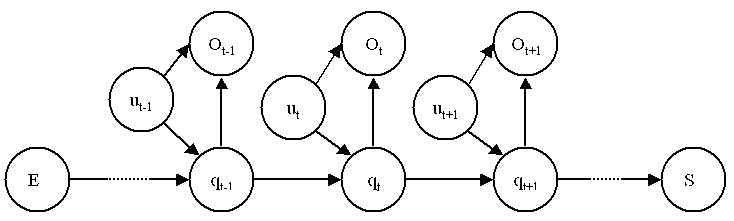
\includegraphics[height=3cm, width=9cm] 
    {\filext{../dessin2/hmm_iohmm}}\end{array}$}$$
    \caption{Illustration d'un IOHMM, les fl�ches indiquent le sens des d�pendances.}
    \label{biblio_hmm_iohmm}
		\end{figure}

					\begin{eqnarray}
					\pr{O \sachant u,M}  &=&     \summyone{\vecteur{q_1}{q_T}}   
																				\pr{O,\vecteurno{q_1}{q_T} \sachant u,M} \nonumber \\
					             &=&     \summyone{\vecteur{q_1}{q_T}}   
					             					\Bigg[ \pr{q_1 \sachant u_1,M} \pr{O_1 \sachant q_1, u_1,M}  \nonumber \\
					             &&      \quad \quad \quad \quad
					                             \prody{t=2}{T} \pr{q_t \sachant u_t, q_{t-1}, M} 
					                             \pr{O_t \sachant u_t, q_t,M}
					                             \Bigg]
					                             \label{biblio_equation_iohmm}
					\end{eqnarray}


La s�quence $u$ est consid�r�e comme l'entr�e du mod�le (input) et $O$ sa sortie (output). Ces mod�les englobent les cha�nes de Markov cach�es (il suffit que le processus $u$ soit constant) et permettent aux transitions de d�pendre d'un processus connu. Dans ce mod�le, la s�quence $\pa{q_t}$ d�pend de la s�quence $\pa{u_t}$, alors que, dans une cha�ne de Markov cach�e, si on remplace la s�quence d'observations $\pa{O_t}$ par $\pa{O_t,u_t}$, les observations $\pa{u_t}$ d�pendent de la s�quence d'�tats $\pa{q_t}$. Les IOHMM inversent en partie cette d�pendance.

Par rapport aux mod�les expos�s dans les paragraphes~\ref{biblio_mmc_classifieur}, \ref{biblio_mmc_gauss}, \ref{biblio_mmc_rn}, et~\ref{biblio_svm}, les IOHMM proposent une alternative pour la cha�ne de Markov cach�e, les discussions relatives au choix du classifieur demeurent.









\subsection{Transducteurs}
\indexfr{transducteur}

Les transducteurs sont assez proches des cha�nes de Markov cach�es puisqu'il est possible de les assimiler � des cha�nes de Markov cach�es d'ordre $\pa{1,1}$ (voir \citeindex{Mohri1996}), c'est-�-dire que l'�mission d'une observation d�pend � la fois de l'�tat courant et de l'�tat pr�c�dent, on dit g�n�ralement que l'�mission se fait sur la transition, ceci se traduit par l'expression (\ref{biblio_equation_transducteur})~:

			\begin{eqnarray}
			\pr{O \sachant M}  &=&     \summyone{\vecteur{q_1}{q_T}}   \pr{O,\vecteurno{q_1}{q_T} \sachant M} \nonumber \\
			\pr{O \sachant M}  &=&     \summyone{\vecteur{q_1}{q_T}}   \cro{\pr{q_1 \sachant M} \pr{O_1 \sachant q_1, M}
			                                                            \prody{t=2}{T} \pr{q_t \sachant q_{t-1}, M} 
			                                                            \pr{O_t \sachant q_t, q_{t-1},M}}
			                                                            \label{biblio_equation_transducteur}
			\end{eqnarray}

La correspondance entre transducteurs et cha�nes de Markov cach�es existe\seeannex{corollaire_chaine_markov_cachee_1}{MMC} sans toutefois conserver le m�me nombre de coefficients. Transducteurs et cha�nes de Markov cach�es sont �quivalents. Encore une fois, par rapport aux mod�les expos�s dans les paragraphes~\ref{biblio_mmc_classifieur}, \ref{biblio_mmc_gauss}, \ref{biblio_mmc_rn}, et~\ref{biblio_svm}, les transducteurs proposent une alternative pour la cha�ne de Markov cach�e, les discussions relatives au choix du classifieur demeurent.










\subsection{Class Hidden Model Markov : CHMM}
\indexfr{CHMM} \indexsee{Class Hidden Model Markov}{CHMM} \label{biblio_mmc_chmm}

Ces mod�les sont d�crits par~\citeindex{Krogh1994} ou~\citeindex{Riis1998}. Le mod�le CHMM $M$ �met une s�quence d'observations $\vecteur{O_1}{O_T}$ ainsi qu'une s�quence de labels $\vecteur{l_1}{l_T}$. Si on note une s�quence d'�tats $\vecteur{q_1}{q_T}$, on obtient~:

    \begin{eqnarray}
      && \pr{\vecteurno{O_1}{O_T},\vecteurno{l_1}{l_T},\vecteurno{q_1}{q_T} |M} \nonumber\\
    = &&            \pr{q_1|M} \pr{O_1|q_1,M} \pr{l_1|q_1,M} \prody{t=2}{T} 
    	  						\pr{q_t|q_{t-1},M} \pr{O_t|q_t,M} \pr{l_t|q_t,M}
    \end{eqnarray}


Si les labels correspondent aux lettres, alors la reconnaissance d'une s�quence d'observations consiste � trouver~:

    \begin{eqnarray}
    \vecteur{l_1^*}{l_t^*} = \underset {\vecteur{l_1}{l_T}} {\arg \max}
                        \crochet{ \summyone{\vecteur{q_1}{q_T}}
                        \pr{\vecteurno{O_1}{O_T},\vecteurno{l_1}{l_T},\vecteurno{q_1}{q_T}  |M} }
    \end{eqnarray}

L'apprentissage peut �tre probl�matique car il demande des s�quences d'observations labellis�es, c'est-�-dire que chaque observation doit �tre associ�e � une lettre. Cette information n'est pas toujours disponible lorsque le nombre de graph�mes diff�re de celui des lettres. Si l'annotation \indexfr{annotation} de chaque image ne contient que le mot �crit dedans sans aucune indication de position des lettres, ces mod�les ne peuvent �tre estim�s.










\subsection{Generalized Markov Models : GMM} 

\indexsee{Generalized Markov Models}{GMM} \indexfr{GMM} 
\indexsee{mod�les de Markov g�n�ralis�s}{GMM}

L'apprentissage de mod�les de Markov cach�s se r�sume � une optimisation sous contrainte puisque les coefficients de ces mod�les doivent �tre des probabilit�s. Cette optimisation peut �tre men�e sans contrainte, les mod�les obtenus sont alors appel�s Generalized Markov Models (\citeindex{Niles1990}, \citeindex{Balasubramanian1993}). L'apprentissage est plus facile mais ces mod�les ne d�finissent plus une loi de probabilit� sur l'espace des observations. Toutefois, Balasubramanian souligne le fait qu'� nombre de coefficients �gal, les GMM semblent �tre de meilleurs classifieurs que les mod�les de Markov cach�s. Le refrain est ensuite le m�me puisque par rapport aux mod�les expos�s dans les paragraphes~\ref{biblio_mmc_classifieur}, \ref{biblio_mmc_gauss}, \ref{biblio_mmc_rn}, et~\ref{biblio_svm}, les GMM proposent une alternative pour la cha�ne de Markov cach�e, les discussions relatives au choix du classifieur demeurent.










\subsection{Arbres de d�cision} 

\indexfrr{arbre}{d�cision}
\label{biblio_geman}

Un autre mod�le de classifieur bas� sur un arbre est propos� par~\citeindex{Amit1997}. \indexfr{arbre} La m�thode d�crite allie � la fois construction d'un arbre de classification et s�lection de caract�ristiques. Les r�ponses positives de plusieurs filtres matriciels (4x4, 16x16 selon la r�solution de l'image) sont recens�es et appel�es "tag". Il est possible de discriminer deux images de caract�res en comparant les distances et les angles form�s par les droites reliant les tags (figure~\ref{blibliographie_geman}).

		\begin{figure}[ht]
    $$\frame{$\begin{array}[c]{c}
    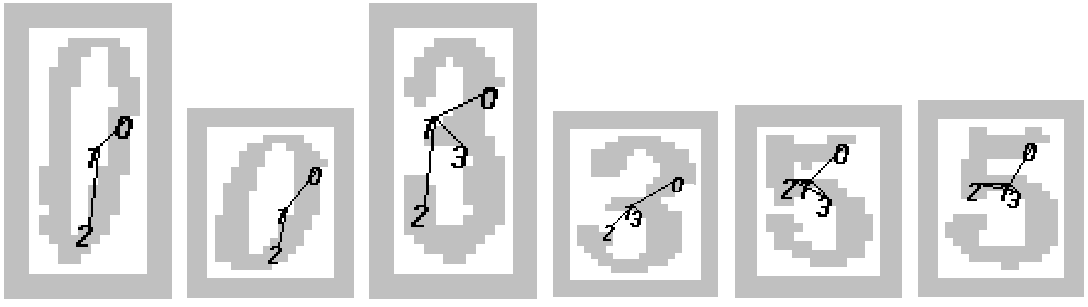
\includegraphics[height=4cm, width=12cm] {\filext{../bibliographie/image/biblio_geman}} \\
    \end{array}$}$$
    \caption{Image extraite de~\citeindexfig{Amit1997}, les tags 0,1,2 sont reconnus dans toutes les images, 
    					les images de "0" sont s�par�es des images de "3" et de "5" par l'absence du tag 3, 
    					les images "3" et "5" sont class�es 
              en comparant les angles entre les arcs reliant les tags. \citeindexfig{Amit1997} propose
              une m�thode permettant de d�terminer les relations discriminantes soit l'ensemble minimal
              de r�gles permettant de classer chaque image de chiffre.
              \citeindexfig{Amit1997}
              }
    \label{blibliographie_geman}
		\end{figure}

La construction d'un tel syst�me passe par un choix ad�quat des tags et des relations qui les unissent afin d'obtenir un syst�me de classification robuste et utilisant le moins de r�gles possible. L'ensemble pr�sent� par~\citeindex{Amit1997} est un reconnaisseur de caract�res mais il pourrait �tre adapt� pour la classification des graph�mes. \indexfr{graph�me} Dans ce cas, ce syst�me est une alternative aux quatre d�j� d�crites dans les paragraphes~\ref{biblio_mmc_classifieur}, \ref{biblio_mmc_gauss}, \ref{biblio_mmc_rn}, et~\ref{biblio_svm}.











\subsection{R�seau de neurones incluant des pr�traitements d'images}
\indexfr{traitement d'image} \indexfr{RN}

Ce syst�me pr�sent� dans~\citeindex{LeCun1998} est un autre reconnaisseur de caract�res bas� sur un r�seau de neurones. Il diff�re des autres par l'incorporation de plusieurs couches de neurones d�volues au traitement d'image (figure~\ref{blibliographie_bengio}). Son apprentissage est aussi diff�rent des autres puisqu'il est appris � partir d'une base d'images de caract�res annot�s et de transformations de ces images (inclinaison, rotation, bruitage,~...).

		\begin{figure}[ht]
    $$\frame{$\begin{array}[c]{c}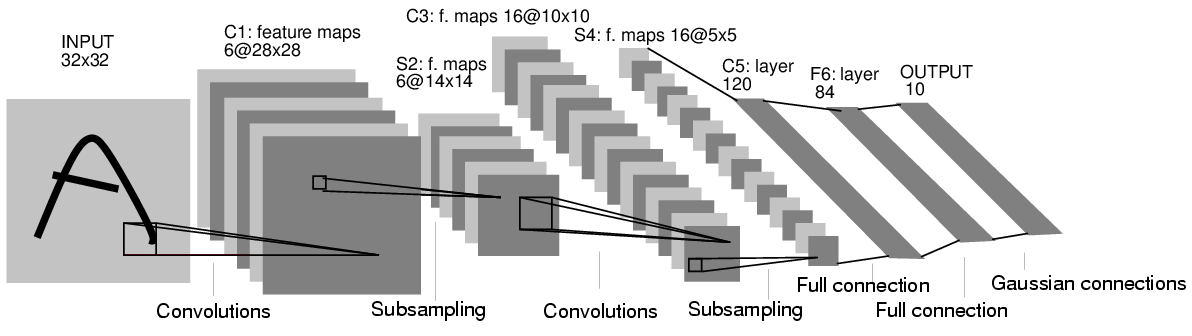
\includegraphics[height=4cm, width=12cm]
    {\filext{../bibliographie/image/biblio_bengio}}\end{array}$}$$
    \caption{Figure extraite de~\citeindexfig{LeCun1998} repr�sentant le r�seau baptis� LeNet-5, 
    						 un r�seau de neurones �
                 convolution pour la reconnaissance de caract�res, tous les plans de la couche C1 partagent
                 les m�mes coefficients, les sorties de cette couche forment un ensemble de caract�ristiques pour la
                 couche suivante puisque directement extraites de l'image.}
    \label{blibliographie_bengio}
		\end{figure}


L'ensemble pr�sent� par~\citeindex{LeCun1998} est un reconnaisseur de caract�res mais il pourrait �tre adapt� pour la classification des graph�mes. \indexfr{graph�me} Dans ce cas, ce syst�me est une autre alternative aux cinq d�j� d�crites dans les paragraphes~\ref{biblio_mmc_classifieur}, \ref{biblio_mmc_gauss}, \ref{biblio_mmc_rn}, \ref{biblio_svm} et~\ref{biblio_geman}.










\subsection{Hidden Neural Network : HNN}
\indexfr{HNN} \indexsee{Hidden Neural Network}{HNN}


Ces mod�les d�velopp�s dans~\citeindex{Riis1998} sont construits autour de r�seaux de neurones classifieurs\seeannex{classification}{classification}. Soit $M$ un HNN poss�dant $N$ �tats, � chaque �tat $q \in \intervalle{1}{N}$ sont associ�s deux r�seaux de neurones $f_q$ et $g_q$ dont les poids sont respectivement $w_q^f$ et $w_q^g$. Soit une s�quence d'observations $\vecteur{O_1}{O_T}$, et $s=\vecteur{s_1}{s_T}$ une autre s�quence, les probabilit�s de transition et d'�mission du mod�le $M$ sont~:

			\begin{eqnarray*}
			\pr{q_t | q_{t-1}, s_{t-1}, M} &=& f_{q_{t-1}}\pa{w_{q_{t-1}}^f, s_{t-1}}\\
			\pr{O_t | q_t, s_{t-1}, M} &=& g_{q_t}\pa{w_{q_t}^g, s_{t-1}}
			\end{eqnarray*}

On en d�duit que, si $\vecteur{q_1}{q_T}$ est une s�quence d'�tats (voir figure~\ref{biblio_figure_hmm_hnn}), alors~:

			\begin{eqnarray}
			\pr{\vecteurno{O_1}{O_T}, \vecteurno{q_1}{q_T} | s,M} = \pr{q_1,s_1,M} 
			\prody{t=2}{T} f_{q_{t-1}}\pa{w_{q_{t-1}}^f, s_{t-1}} g_{q_t}\pa{w_{q_t}^g,
			s_{t-1}}
			\end{eqnarray}

\indexfr{IOHMM}%
Les entr�es $s_t$ des r�seaux des neurones $f_{q_{t-1}}$ et $g_{q_t}$ incluent, comme pour les IOHMM (paragraphe~\ref{biblio_hmm_iohmm}), des informations compl�mentaires mais la s�quence $\vecteur{s_1}{s_T}$ n'est plus discr�te.

Ces mod�les contiennent trop de coefficients pour pouvoir �tre appliqu�s � la reconnaissance de l'�criture car la dimension de l'espace des observations est de quelques dizaines. L'autre inconv�nient de ce mod�le est de ne pas se pr�ter facilement � des modifications d'architecture, une suppression d'�tats entra�ne des changements dans la structure de la cha�ne de Markov cach�e et dans les r�seaux de neurones qui lui sont attach�s.

		\begin{figure}[ht]
    $$\frame{$\begin{array}[c]{c}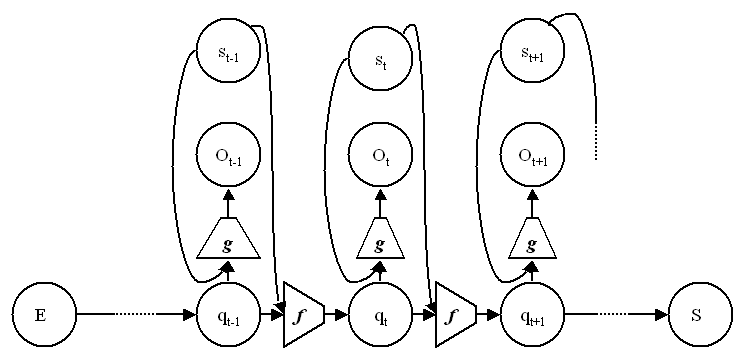
\includegraphics[height=4cm, width=8cm] 
    {\filext{../dessin2/hmm_hnn}}\end{array}$}$$
    \caption{Illustration d'un HNN}
    \label{biblio_figure_hmm_hnn}
		\end{figure}


Ces mod�les sont les plus g�n�raux pr�sent�s, ils englobent les IOHMM qui eux-m�mes englobent les mod�les de Markov cach�s. Ils sont peu utilis�s, leur sont pr�f�r�s les mod�les qui suivent utilisant eux-aussi des r�seaux de neurones mais sont organis�s selon une structure plus simple.










\subsection{Time Delayed Neural Networks : TDNN}
\indexfr{TDNN} \indexsee{Time Delayed Neural Network}{TDNN} \label{blibliographie_tdnn}


Jusqu'� pr�sent, m�me s'ils utilisent des r�seaux de neurones, les mod�les pr�sent�s sont explicitement bas�s sur un squelette incluant le formalisme des cha�nes de Markov. Les mod�les appel�s Time Delay Neural Network ou r�seau de neurones � temps retard�s s'en passent (\citeindex{Schenkel1995}, \citeindex{Senior1994}, \citeindex{Senior1998}). Le principe de ces mod�les illustr�s figures~\ref{biblio_figure_tdnn} est d'�tiqueter chaque observation selon sa classe d'appartenance (ici des classes de lettres) en tenant compte de ses voisins temporels. Ainsi, un TDNN contenant une couche d'entr�e et deux autres couches fonctionnera comme suit~:

    \begin{itemize}
    
    \item La premi�re couche cach�e aura pour entr�es un vecteur de dimension trois fois celle des observations, la s�quence $\vecteur{O_1}{O_T}$ deviendra la s�quence $\vecteur{S_1^1}{S_T^1}$ o� $S_i^1$ est de dimension $D_1$ et $S_t^1 = \pa{O_{t-1},O_t,O_{t+1}}$.
    
    \item La seconde couche aura pour entr�es un vecteur de dimension trois fois $D_1$ et pour sorties un vecteur de probabilit�s $\vecteur{p_1}{p_T}$ correspondant aux classes de sorties des observations $\vecteur{O_1}{O_T}$
    
    \end{itemize}

Ce genre de r�seaux fonctionne comme une fen�tre temporelle locale qui se d�place. Il reste � traiter les effets de bord ou les extr�mit�s de s�quences, pour ce faire, on peut supposer que la s�quence $\vecteur{O_1}{O_T}$ est transform�e en la s�quence $\pa{O_{-1},O_0,\vecteurno{O_1}{O_T},O_{T+1},O_{T+2}}$ o� $O_{-1} = O_0 = O_{T+1} = O_{T+2} = 0$. Cette man\oe uvre est r�p�t�e pour les deux autres couches.


    		\begin{figure}[ht]
        $$\frame{$\begin{array}[c]{c}\includegraphics[height=4cm, width=8cm]
        %{\filext{../bibliographie/image/biblio_tdnn}}\end{array}$}$$
        {\filext{../bibliographie/image/rnnsenior}}\end{array}$}$$
        \caption{Illustration d'un TDNN, figure extraite de \citeindexfig{Senior1994}}
        \label{biblio_figure_tdnn}
    		\end{figure}



Les TDNN associent �troitement forme et s�quence, d�s la premi�re couche, les graph�mes sont consid�r�s avec leur voisinage et ce jusqu'� la derni�re couche qui �tiquettera un graph�me en tenant compte de ses quatre plus proches voisins, qu'ils soient situ�s avant ou apr�s dans la s�quence, ce que ne font pas les mod�les de Markov cach�s qui ne prennent en compte qu'une d�pendance vers le pass�.

L'apprentissage de ces mod�les comme celui des CHMM (voir paragraphe~\ref{biblio_mmc_chmm}) n�cessite l'�tiquetage de chaque graph�me et cette information n'est pas toujours disponible dans les bases de donn�es. C'est pourquoi, ces mod�les n'ont pour le moment pas �t� envisag�s seuls mais plut�t comme simples r�seaux de neurones dans un mod�le hybride comme celui d�crit au paragraphe~\ref{biblio_mmc_rn} o� la cha�ne de Markov cach�e fournit l'annotation\seeannex{hmm_reestimation_rn_classification}{annotation r�seau de neurones}.




\subsection{R�seau de neurones r�current}
\indexfrr{r�seau de neurones}{r�current}  \label{blibliographie_reseau_recurrent}

Le TDNN est compos� de plusieurs couches qui utilisent les r�sultats des pr�c�dentes estim�s sur plusieurs instants cons�cutifs. Le r�seau de neurones r�current utilise comme entr�e l'observation � l'instant $t$ ainsi que des sorties interm�diaires ou finales du r�seau de neurones � l'instant $t-1$ (voir figure~\ref{biblio_figure_tdnn2}, \citeindex{Senior1994}).

    		\begin{figure}[ht]
        $$\frame{$\begin{array}[c]{c}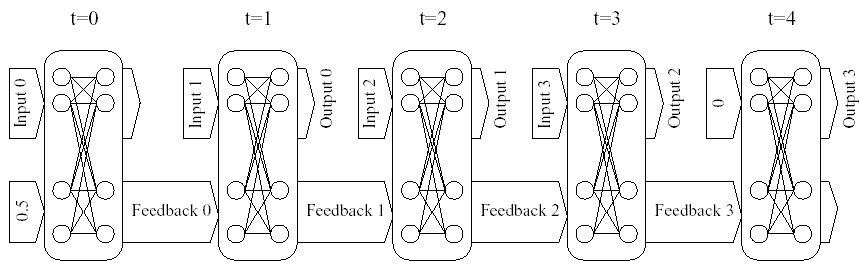
\includegraphics[height=4cm, width=16cm]
        {\filext{../bibliographie/image/tdnnsenior}}\end{array}$}$$
        \caption{Figure extraite de \citeindexfig{Senior1994} illustrant un r�seau de neurones r�currant.}
        \label{biblio_figure_tdnn2}
    		\end{figure}



\indexfr{MMC}

L'article \citeindex{Senior1998} compare les performances obtenues par un TDNN, un r�seau de neurones r�current, un mod�le de Markov cach� seul et un mod�le de Markov cach� hybride associ� � un r�seau de neurones r�currents. Cette derni�re option est la meilleure puisqu'elle permet selon l'auteur d'obtenir un taux d'erreur deux fois moindre par rapport � un r�seau de neurones r�current seul.














\subsection{Mod�le de Markov cach�s 2D}
\label{biblio_hmm_2d_label}

\indexfrr{MMC}{-2D} \indexsee{HMM-2D}{MMC-2D} \indexsee{Hidden Markov Models 2D}{MMC-2D} \indexsee{Mod�les de Markov cach�s 2D}{MMC-2D} \indexfr{quadrillage} \indexfr{pixel} 

Deux versions de ces mod�les sont pr�sent�es, ils diff�rent des cha�nes de Markov cach�es simples (1D) car les observations qu'ils mod�lisent ne sont plus organis�es sous forme de s�quences indic�es temporellement mais sous forme de quadrillage indic� par deux entiers. La figure~\ref{biblio_figure_hmm2d} illustre ce principe dans le cas de la reconnaissance d'un visage. De par cette diff�rence, ces mod�les 2D ne peuvent plus partir des graph�mes ordonn�s sous forme de s�quence mais des pixels eux-m�mes ou d'un d�coupage quadrill� plus grossier.

\indexfr{PHMM} \indexsee{Pattern Hidden Markov Models}{PHMM} \indexsee{HMM 2D}{PHMM} 
\label{blibliographie_phmm}

La premi�re version de ces mod�les sont les Pattern Hidden Markov Models ou PHMM, ils sont bien adapt�s au traitement d'image et sont utilis�s dans la reconnaissance de visages. Leur emploi peut �tre �tendu � la reconnaissance de caract�res (voir \citeindex{Kuo1994}). Il s'agit de mod�le � deux niveaux, le premier niveau est constitu� de super-�tats, chacun associ� � un mod�le de Markov cach� simple (voir~\citeindex{Eickeler1998} et figure~\ref{biblio_figure_hmm2d_2}).

    		\begin{figure}[ht]
        $$\frame{$\begin{array}[c]{c}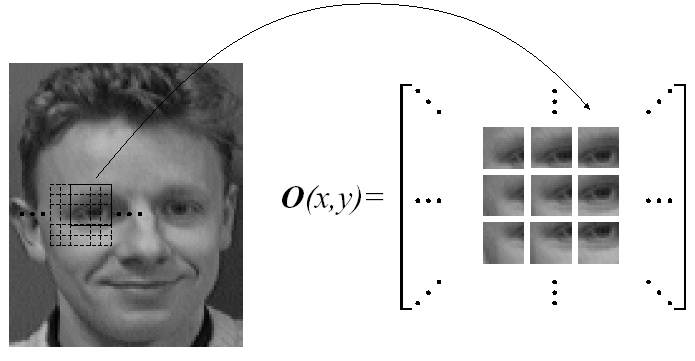
\includegraphics[height=4cm, width=7cm]
        {\filext{../bibliographie/image/biblio_hmm2d_2}}\end{array}$}$$
        \caption{	Figure extraite de~\citeindexfig{Eickeler1998}, observations d'un mod�le de 
        					Markov cach� adapt� � la reconnaissance de visage}
        \label{biblio_figure_hmm2d}
    		\end{figure}

    		\begin{figure}[ht]
        $$\frame{$\begin{array}[c]{c}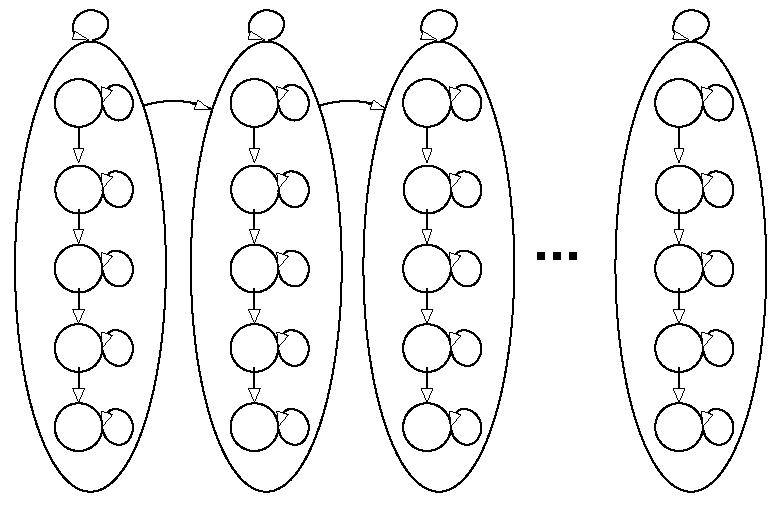
\includegraphics[height=4cm, width=5cm]
        {\filext{../bibliographie/image/biblio_hmm2d}}\end{array}$}$$
        \caption{	Figure extraite de~\citeindexfig{Eickeler1998}, 
        					mod�le de Markov cach� adapt� � la reconnaissance de visage � deux niveaux, 
        					le premier niveau (celui contenant les super-�tats),
                	d�plie les sous-mod�les selon l'axe des abscisses tandis que le second niveau contient des 
                	mod�les dont les �tats se d�plient selon l'axe des ordonn�es.}
        \label{biblio_figure_hmm2d_2}
    		\end{figure}


\indexfr{NSPH-HMM} \indexsee{Non-symmetric Half-Plane Hidden Markov models}{NSPH-HMM}

Une seconde version de ces mod�les est pr�sent�e dans~\citeindex{Saon1997}, ce sont les Non-symmetric Half-Plane Hidden Markov models ou NSPH-HMM. Contrairement au mod�le PHMM, ils ne comportent qu'un niveau. Ils sont caract�ris�s par une matrice d'observations $X=\pa{X_{ij}}_{ \begin{subarray}{c} 1 \infegal i \infegal m \\ 1 \infegal j \infegal n \end{subarray} }$ qui peuvent �tre les pixels eux-m�mes et une cha�ne de Markov cach�e $Q=\pa{q_j}_{1 \infegal j \infegal n }$. On note $\lambda$ les param�tres du mod�le et $\Theta_{ij}$ un voisinage de chaque �l�ment $X_{ij}$ d�fini comme dans la figure~\ref{biblio_figure_hmm2d_theta}.

    \begin{eqnarray*}
    P\pa{X \sachant \lambda}    &=& \summyone{Q} \pr{X,Q \sachant \lambda} \\
                                &=& \summyone{Q} \pr{X \sachant \lambda} \pr{Q \sachant \lambda} \\
                                &=& \summyone{Q} \prody{j=1}{n}  \pr{q_j \sachant q_{j-1}}
                                                 \prody{i=1}{m}  \pr{X_{ij} \sachant X_{\Theta_{ij}}, q_j, \lambda}
    \end{eqnarray*}



    		\begin{figure}[ht]
        $$\frame{$\begin{array}[c]{c}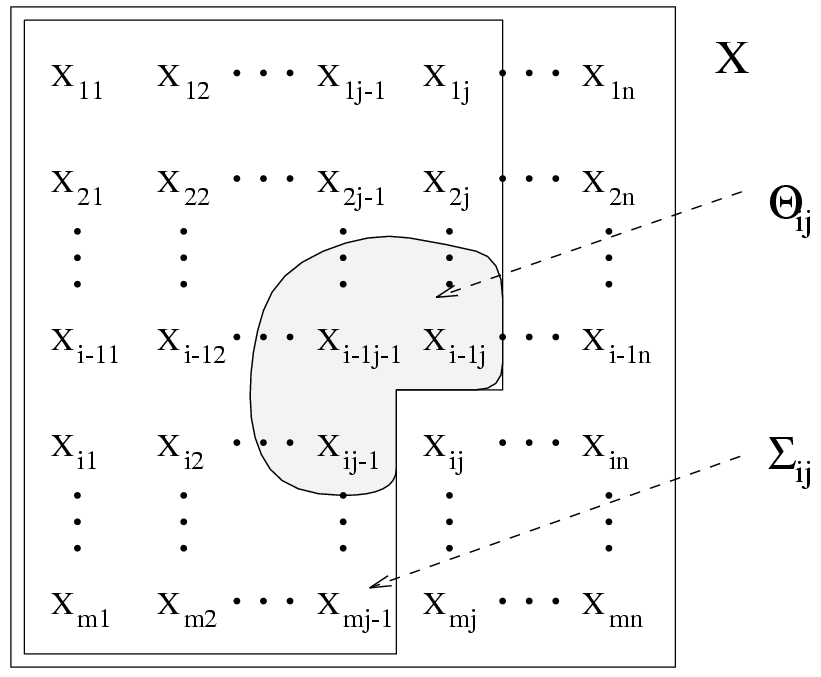
\includegraphics[height=4cm, width=4cm]
        {\filext{../bibliographie/image/biblio_hmm2d_th}}\end{array}$}$$
        \caption{Figure extraite de~\citeindexfig{Saon1997}, voisinage d'un pixel 
        						(ou d'une observation) dans le cas d'un mod�le NSHP-HMM,
                    le voisinage $\Theta_{ij}$ est inclus dans les pixels situ�s � gauche ou au-dessus 
                    d'un pixel $\Sigma_{ij}$.}
        \label{biblio_figure_hmm2d_theta}
    		\end{figure}

Les PHMM diff�rent des NSPH-HMM par le type de d�pendance, dans une seule direction � la fois pour les PHMM, dans les trois quarts du plan pour les NSPH-HMM.







\subsection{Champs de Markov}
\label{biblio_champ_markov}

\indexfr{champs de Markov}\indexfrr{Markov}{champs}\index{d�pendance temporelle}\indexfr{texture}

Jusqu'� pr�sent, les mod�les pr�sent�s utilisent des mod�les de Markov incluant une d�pendance temporelle uniquement tourn�e vers le pass� or, lors du d�cryptage d'un mot, une lettre mal �crite est en g�n�ral d�chiffr�e � l'aide de celles qui l'entourent, autant sur sa droite que sur sa gauche. Il serait donc plus logique que la d�pendance temporelle inclut les caract�res � gauche et � droite. Cette d�pendance n'est plus mod�lisable par une cha�ne de Markov mais par un champ de Markov, mod�les souvent utilis�s pour la mod�lisation de textures. Un tel syst�me de reconnaissance utilisant les champs de Markov est d�crit dans l'article \citeindex{Cai2002} et est compar� � d'autres mod�lisations. Les champs de Markov y obtiennent des performances comparables tout en �tant moins gourmands en terme de coefficients.









%-----------------------------------------------------------------------------------------------------------------
\section{S�lection d'architecture}
%-----------------------------------------------------------------------------------------------------------------
\label{biblio_architecture} \indexsee{architecture}{structure}  \indexfr{structure}  \indexfr{topologie}
\indexfrr{s�lection}{architecture}


Il est facile de choisir entre deux mod�les, il suffit d'estimer leurs param�tres sur une base d'apprentissage comprenant environ 75\% des donn�es puis de comparer leurs performances sur une base de test comprenant environ 25\% des donn�es (\citeindex{Bishop1995}). Cependant, elle est mal adapt�e au probl�me de la reconnaissance car l'apprentissage d'un mod�le est co�teux (une � plusieurs semaines de calculs). Dans ces conditions, la validation crois�e\indexfrr{validation}{crois�e} (\citeindex{Saporta1990}) d'un mod�le est superflue. \citeindex{Bunke1995} envisage quant � lui diff�rentes topologies puis choisit la mieux adapt�e � son probl�me, les architectures envisag�es sont encore dessin�es par celui qui con�oit le syst�me de reconnaissance et ne sont toutefois pas le r�sultat d'un algortihme de s�lection.

Il est donc pr�f�rable d'utiliser des m�thodes qui font �voluer l'architecture des mod�les au cours de l'apprentissage. Pour une mod�lisation donn�e (une de celles propos�es dans les paragraphes~\ref{biblio_modelisation}), il faut trouver le bon nombre d'�tats, le bon nombre de coefficients. 

La figure~\ref{biblio_lettre_g} repr�sente la mod�lisation Markovienne de la lettre 'G', comme l'�criture se lit de gauche � droite, celle-ci ne comporte aucun cycle, mais comment savoir que cette lettre s'�crit avec un ou deux graph�mes~? L'objectif des m�thodes de s�lection d'architecture est d'aboutir au plus petit mod�le capable de repr�senter l'ensemble des donn�es qu'il doit mod�liser, ceci revient � trouver la limite entre~:

    \begin{itemize}
    \item sous-apprentissage : la mod�lisation aboutit � de mauvaises performances en reconnaissance,
            \indexfr{sous-apprentissage}
    \item sur-apprentissage : la mod�lisation est excellente 
    				sur les donn�es apprises mais s'adapte tr�s mal � de nouvelles donn�es.
            \indexfr{sur-apprentissage}  (voir figure~\ref{biblio_equilibre_sur_sous} et \citeindex{Bishop1995})
    \end{itemize}

		    \begin{figure}[ht]
        $$\frame{$\begin{array}[c]{c}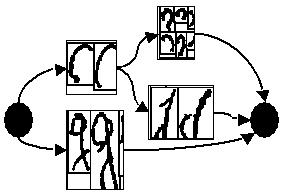
\includegraphics[height=3cm, width=4cm]
        {\filext{../bibliographie/image/biblio_lettre_g}}\end{array}$}$$
        \caption{Mod�lisation de la lettre "G".}
        \label{biblio_lettre_g}
		    \end{figure}

		    \begin{figure}[ht]
		    $$\begin{array}[c]{c}{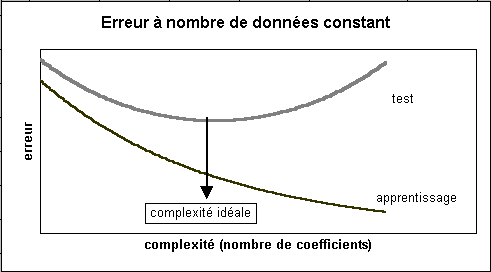
\includegraphics[height=2.0116in, width=3.608in]
		    {\filext{../dessin2/mod_err_test_l_complex}}}\end{array}$$
		    \caption{Equilibre entre sous-apprentissage et sur-apprentissage.}
		    \label{biblio_equilibre_sur_sous}
		    \end{figure}

\indexfrr{base}{test}\indexfrr{base}{apprentissage}

La figure~\ref{biblio_equilibre_sur_sous} sugg�re une d�finition du mod�le optimal~:\indexfrr{mod�le}{optimal} celui qui s'adapte le mieux aux donn�es d'une base de test. Il n'est pas possible d'utiliser cette mesure lors de l'apprentissage auquel cas cette base de test n'en est plus une. La s�lection de l'architecture d'un mod�le doit donc intervenir uniquement � partir des donn�es d'apprentissage. Les paragraphes qui suivent se proposent de jouer avec la structure des mod�les.







\subsection{S�lection de la structure d'un r�seau de neurones}
\indexfrr{s�lection}{r�seau de neurones} \label{biblio_rn_selection}

L'article~\citeindex{Cottrel1995} propose une m�thode permettant d'estimer la pertinence des coefficients d'un r�seau de neurones. Un test statistique (\citeindex{Saporta1990}) permet de tester la nullit� d'un coefficient, de cette mani�re, il est possible de r�duire consid�rablement le nombre de coefficients et d'am�liorer le pouvoir de g�n�ralisation du r�seau. L'inconv�nient de cette m�thode est qu'elle n�cessite la cr�ation d'une matrice carr�e de dimension le nombre de coefficients. Pour de grands r�seaux ($\sim 20000$ coefficients), cette m�thode am�ne quelques difficult�s d'impl�mentation au niveau des capacit�s de stockage en m�moire vive.

Cette s�lection utilise des r�sultats sur les estimateurs du maximum de vraisemblance, ils ne peuvent pas �tre adapt�s tels quels aux mod�les de Markov cach�s car l'estimation de leurs param�tres d�pend d'une optimisation sous contrainte.














\subsection{Estimateur du nombre d'�tats d'une cha�ne de Markov}
\indexfr{estimateur} \indexfr{source de Markov}

L'article \citeindex{Ziv1992} s'int�resse � un estimateur du nombre d'�tats d'une source de Markov, cette famille de mod�les incluant les cha�nes de Markov cach�es. On note $\mathcal{P}_j$ l'ensemble des mod�les dont le nombre d'�tats est inf�rieur ou �gal � $j$, pour une s�quence $x$ de longueur $n$, si $P \in \mathcal{P}_j$, on note $P\pa{x}$ la probabilit� de la s�quence $x$ sachant le mod�le $P$. Par cons�quent, si $S_n$ est l'ensemble des s�quences d'�tats de longueur $n$, alors~:

			$$
			P\pa{x} = \summyone{s \in S_n} \cro{ \pr{x_1, s_1} \prody{i=2}{n} \pr{x_i, s_i \sachant s_{i-1}} }
			$$

On d�finit $N^*$ un estimateur du nombre d'�tats du mod�le $P$~:

			\begin{eqnarray}
			N^* = \min \acc{ j \; \left| \; - \dfrac{1}{n} 
			\ln \cro{\underset{P \in \mathcal{P}_j}{\max} P\pa{x}} - \dfrac{1}{n} U_{LZ}\pa{x} < \lambda
			\right.}
			\end{eqnarray}

$U_{ZL}$ est la longueur en bits du code de Lempel-Ziv (LZ) d�fini dans l'article~\citeindex{Lempel1978}. D'apr�s l'auteur, si $N^*$ est la vraie valeur du nombre d'�tats, cet estimateur v�rifie la condition suivante~: \indexsee{Lempel Ziv}{LZ} \indexfr{LZ}

			\begin{eqnarray}
			\underset{n \longrightarrow \infty}{\lim \inf} \cro{ - \dfrac{1}{n} \ln  \pr{N^* > N} } \supegal \lambda
			\end{eqnarray}

$n$ repr�sente la longueur d'une seule s�quence mais il peut correspondre �galement au nombre de s�quences finies que le mod�le $P$ doit apprendre. Bien que le r�sultat soit int�ressant, le calcul de l'estimateur est encore beaucoup trop co�teux car il n�cessite l'estimation de nombreux mod�les. De plus, ce r�sultat intervient pour des cha�nes de Markov non cach�es.













\subsection{R�duction du nombre de coefficients d'une cha�ne de Markov}
\indexfr{r�duction de coefficients}


Etant donn� que les mots math�matiques sont de longueur finie, il est possible de surestimer le nombre d'�tats optimal n�cessaire � un mod�le afin de les apprendre. \citeindex{Augustin2001} propose une m�thode dont l'initialisation repose sur un mod�le � structure riche (figure~\ref{biblio_hmm_colonne_riche}) auquel vont �tre enlev�s �tats et connexions faibles pour aboutir � une architecture �quivalente et r�duite.

    \begin{figure}[ht]
        $$\frame{$\begin{array}[c]{c}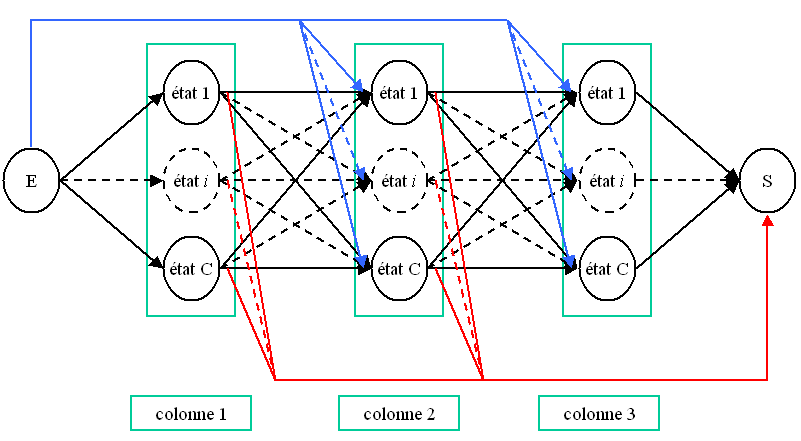
\includegraphics[height=5cm, width=9cm]
        {\filext{../dessin2/selection_emmanuel1}}\end{array}$}$$
        \caption{Un mod�le � structure riche organis� en colonnes}
        \label{biblio_hmm_colonne_riche}
    \end{figure}

Les mod�les utilis�s par~\citeindex{Augustin2001} sont organis�s en colonnes d'�tats, chaque colonne comprend au d�part $C$ �tats o� $C$ est le nombre de classes d'observations et chaque �tat �met une seule classe d'observations
(paragraphe~\ref{biblio_mmc_rn}). La suppression des �tats et connexions faibles est con�ue comme suit~:

    \begin{enumerate}
    
    \item Le mod�le est appris gr�ce aux formules de Baum-Welch 
    			(voir~\citeindex{Levinson1983}, \citeindex{Rabiner1986}).
    
    \item Pour chaque s�quence~:
        \begin{enumerate}
        \item Le meilleur chemin d'�tats est obtenu gr�ce � l'algorithme de
        			 Viterbi\seeannex{paragraphe_viterbi_principe}{Viterbi} 
        			 (voir~\citeindex{Levinson1983}, \citeindex{Rabiner1986}),
        			 il correspond aux �critures les plus probables (voir figure~\ref{biblio_lettre_g}).

        \item Pour chaque connexion, on compte le nombre de meilleurs chemins l'empruntant.
        
        \item On supprime les connexions trop peu utilis�es (en dessous d'un certain seuil), le nombre de connexions supprim�es ne peut �tre sup�rieur � un petit nombre ($\sim 10\%$), les mani�res les moins courantes d'�crire telle ou telle lettre sont oubli�es.
        
        \item Les �tats n'�tant plus connect�s sont supprim�s �galement.
        \end{enumerate}
        
    \item On retourne � l'�tape 1 tant que l'�tape 2 supprime des connexions.
    
    \end{enumerate}

La suppression des connexions s'effectue par �tape, en th�orie, elle devrait s'effectuer une par une, en pratique, pas plus de approximativement 10\% sont supprim�es. Lorsqu'une connexion marginale est supprim�e, une autre qui l'�tait peut ne plus l'�tre pour pallier la disparition de la premi�re, c'est pourquoi, les connexions sont supprim�es petit � petit. La figure~\ref{biblio_hmm_colonne_selection} donne un exemple de r�sultat de cette m�thode.

    		\begin{figure}[ht]
        $$\frame{$\begin{array}[c]{c}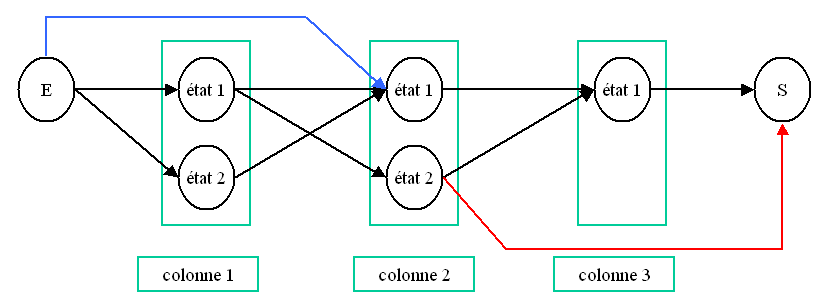
\includegraphics[height=3cm, width=9cm]
        {\filext{../dessin2/selection_emmanuel2}}\end{array}$}$$
        \caption{L'architecture s�lectionn�e par la m�thode d�velopp�e par~\citeindexfig{Augustin2001}}
        \label{biblio_hmm_colonne_selection}
    		\end{figure}







\subsection{Bayesian Information Criterium ou BIC}
\indexfr{BIC}
\indexfr{s�rie temporelle}
\indexfr{auto-r�gressif}

L'article \citeindex{Bicego2003} adapte aux mod�les de Markov cach�s une m�thode fr�quemment utilis�e pour la s�lection de mod�les auto-r�gressifs appliqu�s � la pr�vision de s�ries temporelles. Cette m�thode consiste � pond�rer la vraisemblance, toujours croissante lorsque le nombre de coefficients augmente, par un terme d�croissant. Le mod�le s�lectionn� doit alors maximiser la vraisemblance pond�r�e. Cette m�thode est d�velopp�e au paragraphe~\ref{reco_selection_architecture} qui �voque �galement les probl�mes que soul�ve son adaptation au cas de la reconnaissance de l'�criture.







\subsection{Mod�les de Markov �quivalents}
\indexfr{�quivalence}

L'article \citeindex{Kamp1985} propose une m�thode pour r�duire encore la taille des mod�les de Markov cach�s, elle permet de d�tecter le cas des �tats qui jouent des r�les similaires\seeannex{hmm_select_thoereme_kamp_second}{�tats similaires}~:

\begin{enumerate}
\item les probabilit�s d'�missions de ces �tats sont identiques,
\item le regroupement de ces deux �tats en un seul aboutit � un mod�le �quivalent, deux mod�les $M_1$ et $M_2$ sont dits �quivalents si quelle que soit la s�quence d'observations $O$, $\pr{O \sachant M_1} = \pr{O \sachant M_2}$.
\end{enumerate}

En pratique, l'�quivalence de deux mod�les est v�rifi�e uniquement sur la base ayant servi � estimer les mod�les.

















\subsection{Assemblage de cha�nes de Markov cach�es}
\indexfr{assemblage} \indexfrr{�tat}{non �metteur}


Le formalisme des mod�les de Markov cach�s permet �galement de les assembler de mani�re simple. En introduisant des
�tats non �metteurs (voir~\citeindex{Lallican1999}\seeannex{hmm_intro_entree_sortie}{�tat non �metteur}, un mod�le complexe devient la "somme" de mod�les plus simples comme sur la figure~\ref{biblio_figure_hmm_exemple_modele_imbrique_non_emetteur_deux}.

		\begin{figure}[ht]
    \[\frame{$\begin{array}[c]{c}{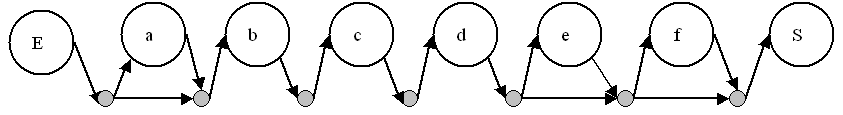
\includegraphics[height=0.6789in,
    width=4.4547in]{\filext{../dessin2/hmm_etat_ne_ex_fin}}}\end{array}$}\]
    \caption{
        Mod�le de mot avec �tats non �metteurs (�tats noirs ainsi que les �tats E (entr�e) et S (sortie)),
        ce mod�le est en quelque sorte une imbrication de mod�les de Markov cach�s not�s (a,b,c,d,e,f) 
        et peut repr�senter les cha�nes
        suivantes~: abcdef, abcd, abcde, abcdf, bcdef, bcd, bcde, bcdf.
    }
    \label{biblio_figure_hmm_exemple_modele_imbrique_non_emetteur_deux}
		\end{figure}

Les �tats non �metteurs sont en quelque sorte des aiguillages, ils n'�mettent pas d'observations, c'est-�-dire que pour une s�quence d'�tats de longueur $T$, une s�quence d'�tats associ�e contiendra $T$ �tats �metteurs et un nombre quelconque d'�tats non �metteurs (de z�ro � l'infini).

Ce formalisme peut �tre utilis� pour construire des mod�les de mots � partir de mod�les de lettres, dans ce cas, vingt-six mod�les de Markov cach�s seulement mod�lisent l'ensemble des mots. Cet assemblage peut �tre adapt� aux IOHMM, \indexfr{IOHMM} aux HNN \indexfr{HNN} et imagin� comme un jeu de lego qui peut r�duire la complexit� des mod�les en �liminant des connexions redondantes. \indexfr{lego} Ce formalisme ne traite pas � proprement parler de la s�lection de mod�les mais il propose un moyen int�ressant d'assembler les mod�les -~ par exemple des mod�les de lettres pour former des mod�les de mots~- sans accro�tre le nombre de coefficients.















%------------------------------------------------------------------------------------------------------------------
\section{Conclusion}
%------------------------------------------------------------------------------------------------------------------
\indexfr{conclusion}
\label{biblio_conclusion}

La mod�lisation sous forme de cha�nes de Markov cach�es est relativement bien adapt�e � la reconnaissance de l'�criture manuscrite. Elle permet de traiter ais�ment des s�quences de petites images. N�anmoins, les recherches sur ces mod�les s'estompent. Outre l'association de mod�les Markov cach�s avec diff�rents types de classifieurs, cette mod�lisation a atteint sa limite sans pour autant �tre v�ritablement d�pass�e par d'autres mod�lisations. Dor�navant, les chercheurs s'orientent plus vers leur inclusion dans un ensemble plus grand et une meilleure utilisation du contexte (voir~\citeindex{Knerr2001}, \citeindex{Koerich2002b}). C'est dans cette direction que ces travaux seront orient�s. 

Cette conclusion s'appuie sur l'article~\citeindex{Steinherz1999} qui consid�re que la reconnaissance de mots cursifs limit�e � un lexique r�duit est un probl�me quasiment r�solu. La recherche est principalement orient�e vers l'optimisation de m�thodes d�j� existantes, ce dont t�moigne la multitude de mod�les inspir�s du formalisme des mod�les de Markov cach�s. Toutefois, bien que pour de grands lexiques les r�sultats obtenus ne soient pas encore satisfaisants, ce m�me article �voque la possibilit� que le probl�me de la seule reconnaissance d'un mot cursif ait atteint sa limite et que dor�navant, elle doive �tre dirig�e vers des post-traitements pouvant inclure des informations contextuelles ou tout simplement l'utilisation de plusieurs classifieurs.\indexfrr{classifieur}{vote} Les HMM et les IOHMM seront les seuls mod�les exp�riment�s. Ce choix peut para�tre arbitraire, il est guid� par le fait que la soci�t� A2iA\indexfr{A2iA} utilise d�j� ces mod�les. 

%Bien que les mod�les de Markov cach�s soient � la base du syst�me de reconnaissance de l'�criture manuscrite d�crit dans ce document, les travaux qui y sont pr�sent�s se situent � leur p�riph�rie. Ils ne s'agit pas de remettre en cause cette mod�lisation mais plut�t de l'am�liorer par des pr�-traitements ou des post-traitements.

Lors d'une reconnaissance, le processus part de l'image en passant par une mod�lisation math�matique avant d'arriver au r�sultat. Les chapitres suivants suivront ce plan, c'est-�-dire la transformation progressive de l'image en un r�sultat de reconnaissance, rappelant les m�thodes d�j� d�velopp�es par d'autres et ins�rant celles qui sont le fruit de ces travaux. Le chapitre suivant est d�di� aux traitements d'images abord�s d'une mani�re plus d�taill�e que dans ce chapitre. Le chapitre d'apr�s est d�di� � la reconnaissance statistique puis viendra le chapitre concernant la d�cision. 

Un dernier chapitre \ref{nouveaux_enjeux} s'int�resse aux nouveaux enjeux, des probl�mes pour lesquels des solutions satisfaisantes commencent � faire leur apparition � partir des ann�es 2004-2005.




\newpage

\firstpassagedo{
	\begin{thebibliography}{99}
	% ins�re une entr�e dans la bibliographie
%		1 - identifiant
%		2 - ann�e
%		3 - auteurs
%		4 - titre
%		5 - revue
%		6 - volume
%		7 - page d�but
%		8 - page fin

\bibitemstyle{Amit1997}{1997}{Y. Amit, D. Geman}
{Shape Quantization and Recognition with Randomized Trees}
{Neural Computation}{9}{1545}{1588}

\bibitemstyle{Augustin2001}{2001}{E. Augustin}
{Reconnaissance de mots manuscrits par syst�mes hybrides r�seaux de neurones et mod�les de Markov cach�s}
{Th�se de l'Universit� Paris V}{}{0}{}

\bibitemstyle{Balasubramanian1993}{1993}{V. Balasubramanian}
{Equivalence and Reduction of Hidden Markov Models}
{Massachussetts Institute of Technology Artificial Intelligence Laboratory}
{A.I. Technical Report No. 1370}{0}{}

\bibitemstyle{Baum1968}{1968}{L. E. Baum L.E., G. R. Sell}
{Growth transformation for functions on manifolds}
{Pac. J. Math.}{27}{211}{227}

\bibitemstyle{Baum1972}{1972}{L. E. Baum}
{An Inequality and Associated Maximization Technique in Statistical Estimation for Probabilistic Functions of a Markov Process}
{Inequalities}{3}{1}{8}

\bibitemstyle{Bengio1992}{1992} {Y. Bengio, R. De Mori, G. Flammia, R. Kompe}
{Global Optimization of a Neural Network-Hidden Markov Model Hybrid}
{IEEE Transactions on Neural Networks}{3(2)}{252}{259}

\bibitemstyle{Bengio1996}{1996} {Y. Bengio, P. Frasconi}
{Input/Output HMMs for sequence processing}
{IEEE Transactions on Neural Network, 7(5)}{1231}{1249}

\bibitemstyle{Bicego2003}{2003}{Manuele Bicego, Vittorio Murino, Mario A.T. Figueiredo}
{A sequential pruning strategy for the selection of the number of states in hidden Markov Models}
{Pattern Recognition Letters}{24}{1395}{1407}

\bibitemstyle{Bishop1995}{1995}{C. M. Bishop}
{Neural networks for pattern recognition}
{Oxford University Press}{}{0}{}

\bibitemstyle{Bottou1991}{1991}{L. Bottou}
{Une approche th�orique de l'apprentissage connexionniste, Application � la reconnaissance de la parole}
{Th�se de l'Universit� dfe Paris Sud, Centre d'Orsay}{}{0}{}

\bibitemstyle{Bunke1995}{1995}{H. Bunke, M. Roth, E. G. Schukat-Talamazzini}
{Off-line cursive handwriting recognition using hidden Markov models}
{Pattern Recognition}{28}{1399}{1413}

\bibitemstyle{Burges1998}{1998}{C. J. C. Burges}
{A tutorial on support vector machines for pattern recognition}
{Data Mining and Knowledge Discovery}{2(2)}{955}{974}

\bibitemstyle{Cai2002}{2002}{Jinhai Cai, Zhi-Qiang Liu}
{Pattern recognition using Markov random field models}
{Pattern Recognition}{35}{725}{733}

\bibitemstyle{Cottrel1995}{1995} {M. Cottrel, B. Girard, M. Mangeas, C. Muller}
{Neural modeling for time series~: a statistical stepwise methode for weight elimination}
{IEEE Transaction On Neural Networks}{6(6)}{0}{}

\bibitemstyle{Dempster1977}{1977} {A. P. Dempster, N. M. Laird, D. B. Rubin}
{Maximum-Likelihood from incomplete data via the EM algorithm}
{Journal of Royal Statistical Society B}{39}{1}{38}

\bibitemstyle{Eickeler1998}{1998} {S. Eickeler, S. M�ller, G. Rigoll}
{Improved Face Recognition Using Pseudo-2D Hidden Markov Models}
{Workshop on Advances in Facial Image Analysis and Recognition Technology in conjunction with 5th
European Conference on Computer Vision (ECCV'98), Freiburg, Germany}{}{0}{}

\bibitemstyle{Kamp1985}{1985} {Y. Kamp}
{State Reduction in Hidden Markov Chains Used for Speech Recognition}
{IEEE Transactions of Acoustics, Speech and Signal Processing}{33 (5)}{1138}{1145}

\bibitemstyle{Knerr2000}{2000}{S. Knerr, P. Lallican, C. Viard-Gaudin}
{From Off-Line to On-Line handwriting Recognition}
{International Workshop on Frontiers in Handwriting Recognition, IWFHR'2000, Amsterdam, The Netherlands}{}{303}{312}

\bibitemstyle{Knerr2001}{2001} {S. Knerr, Y. Tay, P. Lallican, M. Khalid, C. Viard-Gaudin}
{An offline cursive handwritten word recognition system}
{In Proceedings of IEEE Region 10 Conference}{}{0}{}

\bibitemstyle{Koerich2002b}{2002} {A. L. Koerich, R. Sabourin, Y. Leydier, C. Y. Suen}
{A Hybrid Large Vocabulary Handwritten Word Recognition System using Neural Networks with Hidden Markov Models}
{8th International Workshop on Frontiers of Handwriting Recognition (IWFHR'8)}{}{99}{104}

\bibitemstyle{Khorsheed2003}{2003} {M. S. Khorsheed}
{Recognising handwritten Arabic manuscripts unsing a single hidden Markov model}
{Pattern Recognition Letters}{24}{2235}{2242}

\bibitemstyle{Krogh1994}{1994} {A. Krogh}
{Hidden Markov Models for Labeled Sequency}
{Proceeding of the 12th IAPR ICPR'94}{}{140}{144}

\bibitemstyle{Kuo1994}{1994} {S. Kuo, E. Agazzi}
{Keyword Spotting in Poorly Printed Documents Using Pseudo 2-D Hidden Markov Models}
{IEEE Transactions on Pami}{16(8)}{842}{848}

\bibitemstyle{Lallican1999}{1999} {P. M. Lallican}
{Reconnaissance de l'�criture manuscrite hors-ligne~: utilisation de la chronologie restaur�e du trac�}
{Th�se de l'Universit� de Nantes IRESTE}{}{0}{}

\bibitemstyle{Lecolinet1990}{1990} {E. Lecolinet}
{Segmentation d'images de mots manuscrits}
{Th�se de l'Universit� Paris~VI}{}{0}{}

\bibitemstyle{Lecolinet1996}{1996} {E. Lecolinet}
{A Survey of Methods and Strategies in Character Segmentation}
{IEEE Transactions on Pattern Analysis and Machine Intelligence (PAMI)}{18(7)}{690}{706}

\bibitemstyle{LeCun1998}{1998} {Y. Lecun, L. Bottou, Y. Bengio, P. Haffner}
{Gradient-Based Learning Applied to Document Recognition}
{Proceedings of the IEEE}{86 (11)}{2278}{2324}

\bibitemstyle{Lempel1978}{1978} {A. Lempel, J. Ziv}
{Compression of individual sequences via variable rate coding}
{IEEE, Transactions on Information Theory}{IT-24}{530}{536}

\bibitemstyle{Levinson1983}{1983}{S. E. Levinson, L. R. Rabiner, N. M. Sondhi}
{An introduction to the application of the theory of probabilistic functions of a Markov process to automatic speech recognition}
{Bell System Technical Journal}{52 (4)}{257}{285}

%\bibitemstyle{Lin2003}{2003}{Xiafon Lin, Sherif Yacoub, John Burns, Steven Simske}
%{Performance analysis of pattern classifier combination by plurality voting}
%{Pattern Recognition Letters}{24}{1959}{1969}

\bibitemstyle{Mohri1996}{1996}{M. Mohri}
{Finite-state transducers in language and speech processing}
{Computational Linguistics}{20(1)}{1}{33}

\bibitemstyle{Niles1990} {1990}{ L. T. Niles}
{Modelling and Learning in Speech Recognition : the relationship between stochastic pattern classifiers
and neural networks}
{Technical Report LEMS-79, Brown University}{}{0}{}

\bibitemstyle{Rabiner1986}{1986} { L. R. Rabiner, B. H. Juang}
{An introduction to hidden Markov models}
{IEEE ASSP Magazine January}{}{4}{15}

\bibitemstyle{Riis1998}{1998}{S. K. Riis}
{Hidden Markov models and neural networks for speech recognition}
{Th�se de l'Universit� Technique du Danemark}{}{0}{}

\bibitemstyle{Saon1997}{1997}{G. Saon, A. Bela�d}
{High Performance Unconstrained Word Recognition System Combining HMMs and Markov Random Field}
{International Journal on Pattern Recognition and Artificial Intelligence (IJPRAI)}
{Special Issue on Automatic Bankcheck Processing, S. Impedovo Ed. vol. 11, n. 5}{771}{788}

\bibitemstyle{Saporta1990}{1990}{Gilbert Saporta}
{Probabilit�s, analyse des donn�es et statistique}
{Editions Technip}{}{0}{}

\bibitemstyle{Sayre1973}{1973}{ K.  Sayre}
{Machine recognition of handwritten words: a project report}
{Pattern Recognition}{5(3)}{213}{228}

\bibitemstyle{Schenkel1995}{1995}{M. Schenkel, I. Guyon, D. Henderson}
{On-line cursive script recognition using time delay neural networks and hidden Markov models}
{Machine Vision and Applications}{}{215}{223}

\bibitemstyle{Senior1994}{1994}{A. Senior}
{Off-line Cursive Handwriting Recognition using Recurrent Neural Network}
{PHD Thesis in Trinity Hall, Canmbridge, England}{}{0}{}

\bibitemstyle{Senior1998}{1998}{A. Senior}
{An off-line cursive handwriting recognition system}
{IEEE Transactions on Pattern Analysis and Machine Intelligence}{20(3)}{309}{321}

\bibitemstyle{Steinherz1999}{1999}{T. Steinherz, E. Rivlin, N. Intrator}
{Offline cursive script word recognition - a survey}
{Internation Jounral on Document Analysis and Recognition (IJDAR)}{Abstract Volume 2 Issue 2/3}{90}{110}

\bibitemstyle{Simon1992}{1992} {J. C. Simon, O. Baret}
{Cursive words recognition}
{From Pixel to Features III: Frontiers in Handwriting Recognition, S. Impedovo and J.C. Simon (eds.) Elsevier Science Publishers B.V.}{}{241}{260}

\bibitemstyle{Vapnik1979}{1979}{V. N. Vapnik}
{Estimation of dependances based on empirical data}
{(en russe), Nauka, Moscow, 1979, traduction anglaise~: Springer-Verlag, New-York (1982)}{}{0}{}

\bibitemstyle{Verma2004} {2004} {Brijest Verma, Michael Blumenstein, Moumita Glosh}
{A novel approach for structural feature extraction: Contour vs direction}
{Pattern Recognition Letters}{25}{975}{988}

\bibitemstyle{Vinciarelli2002}{2002} {A. Vinciarelli}
{A survey on off-line Cursive Word Recognition}
{Pattern Recognition}{35}{1433}{1446}

\bibitemstyle{Ziv1992}{1992} {J. Ziv, N. Merhav}
{Estimating the number of states of a finite state source}
{IEEE Transactions on Information Theory}{38(1)}{61}{65}


%G. Saon. Mod�les markoviens uni- et bidimensionnels pour la reconnaissance de l��criture manuscrite hors-ligne. PhD thesis, Universit� Henri Poincar� - Nancy I, Vand�uvre-l�s-Nancy, 1997.







	\end{thebibliography}
}

%-----------------------------------------------------------------------------------------------------
% afin d'�viter d'inclure plusieurs ce fichier
%-----------------------------------------------------------------------------------------------------

\ifnum\nbpassages=1



%\newpage
%\footnotesize
%\listoffigures
%\listoftables
%\normalsize
%\newpage



\fi

%
%-----------------------------------------------------------------------------------------------------
% afin d'�viter d'inclure plusieurs ce fichier
%-----------------------------------------------------------------------------------------------------

\ifnum\nbpassages=1

%-----------------------------------------------------------------------------------------------------
% �crit l'index
%-----------------------------------------------------------------------------------------------------
%\chapter{Index}
\begin{flushleft}
\printindex
\end{flushleft}




%-----------------------------------------------------------------------------------------------------
% �crit la table des mati�res de fa�on d�taill�e
%-----------------------------------------------------------------------------------------------------
%\footnotesize
\setcounter{tocdepth}{3}
\tableofcontents%
%\normalsize
%\shorttableofcontents{Table des mati�res d�taill�e}{3}

%-----------------------------------------------------------------------------------------------------
\end{document}
%-----------------------------------------------------------------------------------------------------


\else


\ifnum\nbpassages=2
\nbpassages=1
\fi 

\ifnum\nbpassages=3
\nbpassages=2
\fi 

\ifnum\nbpassages=4
\nbpassages=3
\fi 

\ifnum\nbpassages=5
\nbpassages=4
\fi 


\fi
%

%-----------------------------------------------------------------------------------------------------------
% packages
%------------------------------------------------------------------------------------------------------------


\ifx\firstpassage\undefined
\def\firstpassage{1}
\newcount\nbpassages
\nbpassages=1



%-----------------------------------------------------------------------------------------------------------
% packages
%------------------------------------------------------------------------------------------------------------
%\documentclass[french,11pt]{report}
\documentclass[french,11pt]{../../common/thesis_x}
\usepackage[french]{babel}
\usepackage{a4}
\usepackage[T1]{fontenc}
\usepackage{amsmath}
\usepackage{amssymb}
\usepackage{subfigure}
\usepackage{float}
\usepackage{latexsym}
\usepackage{amsfonts}
\usepackage{epic}
\usepackage{eepic}
\usepackage{makeidx}
\usepackage{multido}
\usepackage{varindex}

\usepackage[lmargin=2cm,rmargin=2cm,tmargin=2cm,bmargin=2cm]{geometry}

\usepackage{graphicx}   %[pdftex]
\usepackage{shorttoc}


%-----------------------------------------------------------------------------------------------------------
% graphics path
%-----------------------------------------------------------------------------------------------------------
%\graphicspath{d:/home/dupre/rapport/these/dessin2}


% note de bas de page : \footnote
% reference (section, theoreme) : \label{a} ... ~\ref{a}...~\pageref{a}
% reference (figure) : \label{a-fig} ... ~\ref{a-fig}...~\pageref{a-fig}
% chapter, section, subsection, ..., plus dans la table des mati�res, ..., subsubsection, paragraph,
% subparagraphe
% cadre : \frame{$ ... $}
% tableau, matrice : \begin{array}{lll} (alignement des colonnes) ... \end{array}
% liste d'�quation non num�rot�es \begin{eqnarray} \\ passage � la ligne, &=& alignement \end{eqnarray}
% index  : \index{cle@ecrit}


%------------------------------------------------------------------------------------------------------------
% marges -------------------------------------------------------------------------------------------------------------
\setlength{\parindent}{0cm} \setlength{\parskip}{1ex} \linespread{1}

%------------------------------------------------------------------------------------------------------------
% index
%------------------------------------------------------------------------------------------------------------
%\varindexIndex
\newcommand{\indexfr}  [1]{\index{#1@#1}}
\newcommand{\indexfrr} [2]{\index{#1@#1!#2@#2}}
\newcommand{\indexfrrr}[3]{\index{#1@#1!#2@#2!#3@#3}}
\newcommand{\indexsee} [2]{\index{#1@#1|see{#2}}}

%------------------------------------------------------------------------------------------------------------
% environnements
%------------------------------------------------------------------------------------------------------------

\newcounter{xctheorem}          [section]
\renewcommand{\thexctheorem}    {\thesection.\arabic{xctheorem}}

%\addtocounter{counter}{value}
\renewcommand{\xpagevalue}{17.6cm}
\newcommand{\xpagevaluedef}{16cm}
\newcommand{\xpagevalueloop}{13cm}


\newenvironment{xremark}[1]
    {   \refstepcounter{xctheorem}\setcounter{theorem}{\value{xctheorem}}
        \indexfrr{remarque}{#1}\textbf{Remarque \thexctheorem : #1}\\*}
    {   }



\newenvironment{sectionunderline}[3]
     {	\begin{tabular}{l} \\ 
     		\begin{tabular}{c|l} \hspace{0.1cm} & \textbf{#1 #2 : #3}\\ & 
     		\begin{minipage}{\xpagevaluedef}}
     {	\end{minipage}\\
      	\end{tabular} \\ \\ \end{tabular}}

\newcommand{\possiblecut}{ 	\end{minipage} \\ \end{tabular} \\ \\
			 	\end{tabular}	\\ 
				\begin{tabular}{l} \\ \begin{tabular}{c|l} \hspace{0.1cm} & \\ 
				& \begin{minipage}{\xpagevaluedef}
			  }


\newenvironment{xthdef}[4]
     {				\refstepcounter{#1}
     					\setcounter{#2}{\value{#1}}
     					\begin{sectionunderline}{#3}{\thexctheorem}{#4}
             	\index{�@�!#3@#3!\thexctheorem}
             	\indexfrr{#3}{#4}
        }
     {\end{sectionunderline}}

\newenvironment{xthdefmine}[4]
     {				\refstepcounter{#1}
     					\setcounter{#2}{\value{#1}}
     					\begin{sectionunderline}{#3}{\thexctheorem}{#4}
             	\index{�@�!#3@#3!\thexctheorem}
             	\indexfrr{#3}{#4}
        }
     {\end{sectionunderline}}



%------------------------------------------------------------------------------------------------------------
% instances d'environnements
%------------------------------------------------------------------------------------------------------------

\newenvironment{xtheorem}[1]
		{\begin{xthdef}{xctheorem}{theorem}{Th�or�me}{#1}}{\end{xthdef}}

\newenvironment{xcorollary}[1]
		{\begin{xthdef}{xctheorem}{theorem}{Corollaire}{#1}}{\end{xthdef}}
		
\newenvironment{xlemma}[1]
		{\begin{xthdef}{xctheorem}{theorem}{Lemme}{#1}}{\end{xthdef}}

\newenvironment{xproposition}[1]
		{\begin{xthdef}{xctheorem}{theorem}{Proposition}{#1}}{\end{xthdef}}

\newenvironment{xproperty}[1]
		{\begin{xthdef}{xctheorem}{theorem}{Propri�t�}{#1}}{\end{xthdef}}

\newenvironment{xdefinition}[1]
		{\begin{xthdef}{xctheorem}{theorem}{D�finition}{#1}}{\end{xthdef}}

\newenvironment{xalgorithm}[1]      
		{\setcounter{cxalgostep}{0}
     \begin{xthdef}{xctheorem}{theorem}{Algorithme}{#1}}{\end{xthdef}}
                                    
\newenvironment{xproblem}[1]
		{\begin{xthdef}{xctheorem}{theorem}{Probl�me}{#1}}{\end{xthdef}}

\newenvironment{xtest}[1]
    {\setcounter{cxalgostep}{0}
     \begin{xthdef}{xctheorem}{theorem}{Test}{#1}}{\end{xthdef}}


%------------------------------------------------------------------------------------------------------------
% autres instances d'environnements
%------------------------------------------------------------------------------------------------------------

\newenvironment{xtheoremmine}[1]
		{\begin{xthdefmine}{xctheorem}{theorem}{Th�or�me}{#1}}{\end{xthdefmine}}

\newenvironment{xcorollarymine}[1]
		{\begin{xthdefmine}{xctheorem}{theorem}{Corollaire}{#1}}{\end{xthdefmine}}
		
\newenvironment{xlemmamine}[1]
		{\begin{xthdefmine}{xctheorem}{theorem}{Lemme}{#1}}{\end{xthdefmine}}

\newenvironment{xpropositionmine}[1]
		{\begin{xthdefmine}{xctheorem}{theorem}{Proposition}{#1}}{\end{xthdefmine}}

\newenvironment{xpropertymine}[1]
		{\begin{xthdefmine}{xctheorem}{theorem}{Propri�t�}{#1}}{\end{xthdefmine}}

\newenvironment{xdefinitionmine}[1]
		{\begin{xthdefmine}{xctheorem}{theorem}{D�finition}{#1}}{\end{xthdefmine}}

\newenvironment{xalgorithmmine}[1]      
		{\setcounter{cxalgostep}{0}
     \begin{xthdefmine}{xctheorem}{theorem}{Algorithme}{#1}}{\end{xthdefmine}}
                                    
\newenvironment{xproblemmine}[1]
		{\begin{xthdefmine}{xctheorem}{theorem}{Probl�me}{#1}}{\end{xthdefmine}}

\newenvironment{xtestmine}[1]
    {\setcounter{cxalgostep}{0}
     \begin{xthdef}{xctheorem}{theorem}{Test}{#1}}{\end{xthdefmine}}
     
%------------------------------------------------------------------------------------------------------------
% d�finitions (rectangles noirs, blancs)
%------------------------------------------------------------------------------------------------------------

%%%% debut macro %%%%
\def\sqw{\hbox{\rlap{\leavevmode\raise.3ex\hbox{$\sqcap$}}$\sqcup$}}
\def\sqb{\hbox{\hskip5pt\vrule width4pt height6pt depth1.5pt\hskip1pt}}

% Rectangle noir:
\def\qed{\ifmmode\hbox{\hfill\sqb}\else{\ifhmode\unskip\fi%
\nobreak\hfil \penalty50\hskip1em\null\nobreak\hfil\sqb
\parfillskip=0pt\finalhyphendemerits=0\endgraf}\fi}
% Rectangle blanc:
\def\cqfd{\ifmmode\sqw\else{\ifhmode\unskip\fi\nobreak\hfil
\penalty50\hskip1em\null\nobreak\hfil\sqw
\parfillskip=0pt\finalhyphendemerits=0\endgraf}\fi}
%%%% fin macro %%%%

%------------------------------------------------------------------------------------------------------------
% d�monstrations
%------------------------------------------------------------------------------------------------------------

\newcommand{\legenddemotype}{none}
\newcommand{\legenddemotypeindex}{none}
\newcommand{\legenddemonumber}{none}
\newcounter{cxdemonstration}
\newcounter{cxdemonstrationnumnum}
\renewcommand{\thecxdemonstration}    			{\Alph{cxdemonstration}}
\renewcommand{\thecxdemonstrationnumnum}    {\thesection+\arabic{cxdemonstrationnumnum}}

\newenvironment{xdemo}[2]
    {   \setcounter{cxdemonstration}{0}
    		\refstepcounter{cxdemonstrationnumnum}
        \renewcommand{\legenddemotype}{#1}
        \renewcommand{\legenddemotypeindex}{#1}\renewcommand{\legenddemonumber}{#2}
        \index{�@�!demonstration@d�monstration!#1\thecxdemonstrationnumnum						% #1~#2
        																					@#1~#2}
        \textbf{D�monstration (#1~#2) :}\newline}
    {   
        \hfill{}\textbf{ (\legenddemonumber)}\cqfd}

\newenvironment{xdemomine}[2]
    {   \setcounter{cxdemonstration}{0}
    		\refstepcounter{cxdemonstrationnumnum}
        \renewcommand{\legenddemotype}{#1}
        \renewcommand{\legenddemotypeindex}{#1}\renewcommand{\legenddemonumber}{#2}
        \index{�@�!demonstration@d�monstration!#1\thecxdemonstrationnumnum							% #1~#2$^*$
        																						@#1~#2}
        \textbf{D�monstration (#1~#2) :}\newline}
    {   
        \hfill{}\textbf{ (\legenddemonumber)}\cqfd}


\newcommand{\itemdemo}{\refstepcounter{cxdemonstration}\textbf{Partie \thecxdemonstration~(d�monstration de \legenddemonumber)}\medskip}


%------------------------------------------------------------------------------------------------------------
% environnements initiaux
%------------------------------------------------------------------------------------------------------------

\newtheorem{theorem}                    {\textbf{Th�or�me}}       [section]
\newtheorem{corollary}      [theorem]   {\textbf{Corollaire}}
\newtheorem{lemma}          [theorem]   {\textbf{Lemme}}
\newtheorem{proposition}    [theorem]   {\textbf{Proposition}}
\newtheorem{property}       [theorem]   {\textbf{Propri�t�}}
\newtheorem{definition}     [theorem]   {\textbf{D�finition}}
\newtheorem{algorithm}      [theorem]   {\textbf{Algorithme}}

%------------------------------------------------------------------------------------------------------------
% compteurs d'�tapes dans les algorithmes
%------------------------------------------------------------------------------------------------------------

\newcounter{cxalgostep}
\newcounter{cxloopdegre}[cxalgostep]
\renewcommand{\thecxalgostep}    {\Alph{cxalgostep}}
\renewcommand{\thecxloopdegre}   {\backslash captiondegre\Alph{cxalgostep}}

\newcommand{\captiondegreA}{no}
\newcommand{\captiondegreB}{no}
\newcommand{\captiondegreC}{no}
\newcommand{\captiondegreD}{no}
\newcommand{\captiondegreE}{no}
\newcommand{\captiondegreF}{no}

%------------------------------------------------------------------------------------------------------------
% boucles for, while, test if...
%------------------------------------------------------------------------------------------------------------

\newcommand{\itemalgo}[1]{\refstepcounter{cxalgostep}\textbf{Etape \thecxalgostep~: #1}\newline}

\newenvironment{xloop}
    {   \addtocounter{cxloopdegre}{1}
            \begin{tabular}{cl} \quad & \begin{minipage}{\xpagevalueloop} }
    {   \end{minipage} \end{tabular}
            \addtocounter{cxloopdegre}{-1}}

\newenvironment{xfor}[3]
    {   \textbf{pour $#1 = #2$ � $#3$ faire} \newline%
        \begin{xloop} }
    {   \end{xloop}
        \textbf{fin pour} }

\newenvironment{xfor2}[3]
    {   \textbf{pour $#1 = #2$ � $#3$ faire} \newline%
        \begin{xloop} }
    {   \end{xloop} \newline
        \textbf{fin pour} }

\newenvironment{xforeach}[2]
    {   \textbf{pour chaque $#1 \in #2$ faire} \newline%
        \begin{xloop} }
    {   \end{xloop}
        \textbf{fin pour} }
 

\newcommand{\xdowhilecondition}{no}
\newenvironment{xdowhile}[1]
    {   \renewcommand{\xdowhilecondition}{#1}
        \textbf{faire} \newline%
        \begin{xloop} }
    {   \end{xloop}
        \textbf{tant que (\xdowhilecondition)} }

\newenvironment{xwhile}[1]
    {   \textbf{tant que (#1) faire} \newline%
        \begin{xloop} }
    {   \end{xloop}
        \textbf{fin tant que} }

\newenvironment{xif}[1]
    {   \textbf{si #1 alors} \newline%
        \begin{xloop} }
    {   \end{xloop}
        \textbf{fin si} }
\newcommand{\xelse}{\end{xloop}\textbf{sinon}\newline\begin{xloop}}
\newcommand{\xelseif}[1]{\end{xloop}\textbf{sinon si #1}\newline\begin{xloop}}

\newenvironment{xalgostep}[1]
    {   \refstepcounter{cxalgostep}\textbf{Etape \thecxalgostep~: #1}\newline%
        \begin{xloop} }
    {   \end{xloop}\medskip}
    
%------------------------------------------------------------------------------------------------------------
% fonctions
%------------------------------------------------------------------------------------------------------------

\newcommand{\parenthese}[1]{\left(#1\right)}
\newcommand{\pa}[1]{\left(#1\right)}
\newcommand{\bigpa}[1]{\big( #1 \big)}
\newcommand{\biggpa}[1]{\Big( #1 \Big)}
\newcommand{\bigggpa}[1]{\bigg( #1 \bigg)}
\newcommand{\biggggpa}[1]{\Bigg( #1 \Bigg)}

\newcommand{\scal}[1]{\left<#1\right>}

\newcommand{\abs}[1]{\left|#1\right|}
\newcommand{\bigabs}[1]{\big|#1\big|}
\newcommand{\biggabs}[1]{\bigg|#1\bigg|}

\newcommand{\accolade}[1]{\left\{#1\right\}}
\newcommand{\acc}[1]{\left\{#1\right\}}
\newcommand{\bigacc}[1]{\big\{#1\big\}}
\newcommand{\biggacc}[1]{\Big\{#1\Big\}}
\newcommand{\bigggacc}[1]{\bigg\{#1\bigg\}}
\newcommand{\biggggacc}[1]{\Bigg\{#1\Bigg\}}

\newcommand{\crochet}[1]{\left[#1\right]}
\newcommand{\cro}[1]{\left[#1\right]}
\newcommand{\bigcro}[1]{\big[ #1 \big]}
\newcommand{\biggcro}[1]{\Big[ #1 \Big]}
\newcommand{\bigggcro}[1]{\bigg[ #1 \bigg]}
\newcommand{\biggggcro}[1]{\Bigg[ #1 \Bigg]}
\newcommand{\crochetopen}[1]{\left]#1\right[}

\newcommand{\indicatrice}[1]{\mathbf{1\!\!1}_{\accolade{#1}}}

\newcommand{\ensemblereel}[0]{\mathbb{R}}
\newcommand{\R}[0]{\mathbb{R}}

\newcommand{\ensembleentier}[0]{\mathbb{N}}
\newcommand{\N}[0]{\mathbb{N}}

\newcommand{\infegal}[0]{\leqslant}
\newcommand{\supegal}[0]{\geqslant}

\newcommand{\intervalle}[2]{\left\{#1,\cdots,#2\right\}}
\newcommand{\intervalleinf}[3]{#1 \infegal #2 \infegal #3}

\newcommand{\loinormale}[2]{{\cal N} \parenthese {#1,#2}}
\newcommand{\loibinomiale}[2]{{\cal B} \parenthese {#1,#2}}
\newcommand{\loimultinomiale}[1]{{\cal M} \parenthese {#1}}
\newcommand{\loi}[0]{{\cal L}}

\newcommand{\dans}[0]{\longrightarrow}

\newcommand{\demonstration}[0]{\bigskip\textbf{D�monstration :}\bigskip}

\newcommand{\partialfrac}[2]{\frac{\partial #1}{\partial #2}}

\newcommand{\summy}[2]{\overset{#2}{\underset{#1}{\sum}}}
\newcommand{\bigsummy}[2]{\overset{#2}{\underset{#1}{\displaystyle\sum}}}
\newcommand{\prody}[2]{\overset{#2}{\underset{#1}{\prod}}}
\newcommand{\bigprody}[2]{\overset{#2}{\underset{#1}{\displaystyle\prod}}}
\newcommand{\summyone}[1]{\underset{#1}{\sum}}
\newcommand{\bigsummyone}[1]{\underset{#1}{\displaystyle\sum}}
\newcommand{\prodyone}[1]{\underset{#1}{\prod}}

\newcommand{\card}[1]{card \parenthese{#1}}

\newcommand{\esperance}[1]{\mathbb{E}\parenthese{#1}}
\newcommand{\esperanceseul}[0]{\mathbb{E}\,}
\newcommand{\esp}[1]{\mathbb{E}\pa{#1}}
\newcommand{\esps}[0]{\mathbb{E}\,}

\newcommand{\variance}[1]{\mathbb{V}\parenthese{#1}}
\newcommand{\varianceseul}[0]{\mathbb{V}\,}
\newcommand{\var}[1]{\mathbb{V}\pa{#1}}
\newcommand{\vars}[0]{\mathbb{V}\,}

\newcommand{\pr}[1]{\mathbb{P}\pa{#1}}

\newcommand{\norme}[1]{\left\Vert#1\right\Vert}

\newcommand{\independant}[0]{\;\makebox[3ex]{
					\makebox[0ex]{\rule[-0.2ex]{3ex}{.1ex}}
					\!\!\!\!\makebox[.5ex][l]{\rule[-.2ex]{.1ex}{2ex}}
									\makebox[.5ex][l]{\rule[-.2ex]{.1ex}{2ex}}} \,\,}

\newcommand{\vecteur}[2]{\pa{#1,\dots,#2}}
\newcommand{\vecteurno}[2]{#1,\dots,#2}

\newcommand{\union}[2]{\overset{#2}{\underset{#1}{\bigcup}}}
\newcommand{\unionone}[1]{\underset{#1}{\bigcup}}

\newcommand{\para}[1]{\bigskip\textbf{#1}}
\newcommand{\QARRAY}[2]{\left \{ \begin{array}{l} #1 \\ #2 \end{array} \right .}
\newcommand{\QARRAYno}[2]{\left . \begin{array}{l} #1 \\ #2 \end{array} \right .}
\newcommand{\sachant}{\; | \;}
\newcommand{\itemm}[0]{\item[\quad -]}
\newcommand{\ensemble}[2]{\acc{#1,\dots,#2}}

\newcommand{\twoindices}[2]{\begin{subarray}{c} #1 \\ #2 \end{subarray}}
\newcommand{\vecteurim}[2]{\pa{\begin{subarray}{c} #1 \\ #2 \end{subarray}}}
\newcommand{\vecteurimm}[2]{\pa{\begin{array}{c} #1 \\ #2 \end{array}}}

\newcommand{\sac}{\sachant}
\newenvironment{eqnarrays} {\begin{eqnarray}}{\end{eqnarray}}

\newcommand{\matfour}[4] {\begin{array}{cc} #1 & #2 \\ #3 & #4 \end{array}}
\newcommand{\vectt}[2]{\pa{\begin{subarray}{c} #1 \\ #2 \end{subarray}}}

%\newcommand{\fleche}[1]{\overset{\longrightarrow}{ #1 }}
\newcommand{\fleche}[1]{\overrightarrow{ #1 }}
\newcommand{\inte}{\displaystyle\int}

%------------------------------------------------------------------------------------------------------------
% fonctions sp�ciales
%------------------------------------------------------------------------------------------------------------

% �crire soi-m�me le num�ro d'une �quation
\newcommand{\numequation}[0]{\stepcounter{equation}(\theequation)}		

% nouvel environnements eqnarray
\newenvironment{eqnarray_xd}
    {$$\left\{\begin{array}{rclr}}
    {\end{array}\right.$$}

% red�finition de l'environnement eqnarray
\makeatletter
\newlength{\earraycolsep}
\setlength{\earraycolsep}{2pt}
\def\eqnarray{\stepcounter{equation}\let\@currentlabel%
\theequation \global\@eqnswtrue\m@th \global\@eqcnt\z@\tabskip\@centering\let\\\@eqncr
$$\halign to\displaywidth\bgroup\@eqnsel\hskip\@centering
$\displaystyle\tabskip\z@{##}$&\global\@eqcnt\@ne \hskip 2\earraycolsep \hfil$\displaystyle{##}$\hfil &\global\@eqcnt\tw@ \hskip 2\earraycolsep
$\displaystyle\tabskip\z@{##}$\hfil \tabskip\@centering&\llap{##}\tabskip\z@\cr} \makeatother
    
% ajoute une page afin que la page suivante soit une page au num�ro impair   
\newcommand{\skippairpage}[0]{
	\ifx\xpagepairdoc\undefined
	\newcount\xpagepairdoc
	\fi
	\xpagepairdoc=\value{page}
	\divide\xpagepairdoc by 2
	\multiply\xpagepairdoc by 2
	\ifnum\xpagepairdoc=\value{page}
	\hbox{}\newpage
	\fi
}

%------------------------------------------------------------------------------------------------------------
% dessin
%------------------------------------------------------------------------------------------------------------

\newcounter{putx}
\newcounter{puty}

% dessin d'un arc sup�rieur : x,y,size
\newcommand{\arcup}[3]{
                                \put(#1,#2){\arc{#3}{2.3}{6.8}}
                                \setcounter{putx}{#1}\addtocounter{putx}{6}
                                \setcounter{puty}{#2}\addtocounter{puty}{-4}
                                \put(\value{putx},\value{puty}){\vector(0,-1){1}}
                      }
                      
% dessin d'un arc inf�rieur : x,y,size
\newcommand{\arcdown}[3]{
                                \put(#1,#2){\arc{#3}{5.8}{10.5}}
                                \setcounter{putx}{#1}\addtocounter{putx}{6}
                                \setcounter{puty}{#2}\addtocounter{puty}{3}
                                \put(\value{putx},\value{puty}){\vector(0,1){1}}
                        }
% dessin un rectangle
\newcommand{\drawbox}[4]{\drawline(#1,#2)(#3,#2)(#3,#4)(#1,#4)(#1,#2)}


%------------------------------------------------------------------------------------------------------------
% r�f�rence
%------------------------------------------------------------------------------------------------------------

% d�fini un op�rateur dont le nom est pass� en argumant
\newcommand{\setoperator}[1]{\expandafter\xdef\csname meop@#1\endcsname{1}}
	
% si un op�rateur dont le nom est pass� en 1 est d�fini, alors
% fait 2 sinon fait 3
\newcommand{\testoperator}[3]{\expandafter\ifx\csname meop@#1\endcsname\relax#3\else#2\fi}


% ne pas utiliser dans les figures
\newcommand{\citeindex}[1]		{\cite{#1}\indexfrr{r�f�rences}{#1}\testoperator{cite@#1}{}{\setoperator{cite@#1}}}

% utiliser dans les figures
\newcommand{\citeindexfig}[1]	{\cite{#1}\indexfrr{r�f�rences}{#1}}
															
\newcommand{\bibitemindex}[1]	{\indexfrr{r�f�rences}{#1} \bibitem[#1]{#1}	}

\newcount\bibitemstylefirstpage

% d�finit un compteur pour une ann�e
\newcommand{\counterbiblioyear}[1]{\newcounter{meopyear@#1}\setcounter{meopyear@#1}{0}}
% ajoute une r�f�rence pour une ann�e
\newcommand{\counterbiblioyearadd}[1]{\addtocounter{meopyear@#1}{1}}
% obtient le nombre de documents cit�s pour une ann�e
\newcommand{\counterbiblioyeardisp}[1]{\arabic{meopyear@#1}}

% d�finit un compteur pour une revue
\newcommand{\counterbibliosource}[1]{\newcounter{meopsource@#1}\setcounter{meopsource@#1}{0}}
% ajoute une r�f�rence pour une revue
\newcommand{\counterbibliosourceadd}[1]{\addtocounter{meopsource@#1}{1}}
% obtient le nombre de documents cit�s pour une revue
\newcommand{\counterbibliosourcedisp}[1]{\arabic{meopsource@#1}}

\newcounter{nbcitations}				% compteur pour le nombre de citations
\setcounter{nbcitations}{0}			% aucune citations pour commencer

% ins�re une entr�e dans la bibliographie
%		1 - identifiant
%		2 - ann�e
%		3 - auteurs
%		4 - titre
%		5 - revue
%		6 - volume
%		7 - page d�but
%		8 - page fin
% rappel : 					 			\newcommand{\setoperator}[1]{\expandafter\xdef\csname meop@#1\endcsname{1}}
%													\newcommand{\testoperator}[3]{\expandafter\ifx\csname meop@#1\endcsname\relax#3\else#2\fi}

\newcommand{\bibitemstyle}[8]{  
				\testoperator{yc#2}	{	
				}	
				{		\setoperator{yc#2}
						\counterbiblioyear{#2}
  			}
				%\testoperator{rc#5}	{	
				%}	
				%{		\setoperator{rc#5}
			  %\counterbibliosource{#5}
  			%}
				\testoperator{#1}	{	
					\bibitem[#1]{#1} - cit� aussi page~\pageref{bibpage@#1}
					
						\testoperator{cite@#1}{}{ \textbf{- jamais cit� -} }
						#3, \textit{#4}, #5 #6 %
						\ifnum\bibitemstylefirstpage=0%
						(#2)%
						\else%
						(#2), pp #7-#8%
						\fi%
					
				}	
				{	  \bibitemstylefirstpage=#7
						\counterbiblioyearadd{#2}
						%\counterbibliosourceadd{#5}
						\addtocounter{nbcitations}{1}
						\setoperator{#1}
						\label{bibpage@#1}
						\bibitemindex{#1}
						\testoperator{cite@#1}{}{ \textbf{- jamais cit� -} }
						#3, \textit{#4}, #5 #6 %
						\ifnum\bibitemstylefirstpage=0%
						(#2)%
						\else%
						(#2), pp #7-#8%
						\fi%
  			}
}


\newcommand{\bibinserttitle}[1]{ \bibitem{} \medskip \medskip \begin{huge} \textbf{#1} \end{huge} \medskip \medskip }

%------------------------------------------------------------------------------------------------------------
% annexe
%------------------------------------------------------------------------------------------------------------

% voir les annexes : label, marques dans l'index
\newcommand{\seeannex}[2]{\indexfrr{r�f�rences aux annexes}{#2}\footnote{Annexes~: voir paragraphe~\ref{#1}, page~\pageref{#1}}}


%------------------------------------------------------------------------------------------------------------
% image
%------------------------------------------------------------------------------------------------------------

\newcount \filextensionnum
\filextensionnum = 0

			\filextensionnum=2 \correctionenonce=1 


\ifnum \filextensionnum = 1
\newcommand{\filext}[1]{#1.eps}
\newcommand{\filefig}[1]{\input{#1.tex}}
\else
\newcommand{\filext}[1]{#1.pdf}
\newcommand{\filefig}[1]{\includegraphics{#1.pdf}}
%\usepackage[latin1]{inputenc}
\usepackage{hyperref}  %lien en PDF
\fi

%------------------------------------------------------------------------------------------------------------
% test pour savoir si c'est le premier passage
%------------------------------------------------------------------------------------------------------------
\newcommand{\firstpassagedo}[1]{ \ifnum\nbpassages=1 #1 \fi }

%------------------------------------------------------------------------------------------------------------
% commentaire
%------------------------------------------------------------------------------------------------------------
\newcommand{\comment}[1]{  }



%------------------------------------------------------------------------------------------------------------
% segmentations douloureuses
%------------------------------------------------------------------------------------------------------------
\hyphenation{ap-pren-tis-sa-ge}

%-----------------------------------------------------------------------------------------------------------
% profondeur de la table des mati�res
%-----------------------------------------------------------------------------------------------------------
\setcounter{tocdepth}{3}     % Dans la table des matieres
\setcounter{secnumdepth}{3}  % Avec un numero.

%-----------------------------------------------------------------------------------------------------------
% pr�voit de faire un index 
%-----------------------------------------------------------------------------------------------------------

\makeindex

%-----------------------------------------------------------------------------------------------------------
% document 
%-----------------------------------------------------------------------------------------------------------
\begin{document}


\else

\ifnum\nbpassages=4
\nbpassages=5
\fi 

\ifnum\nbpassages=3
\nbpassages=4
\fi 

\ifnum\nbpassages=2
\nbpassages=3
\fi 

\ifnum\nbpassages=1
\nbpassages=2
\fi 



\fi
%
\firstpassagedo{% ------------------------------------------------------------------------------------------------------------------------------------
% titre ------------------------------------------------------------------------------------------------------------------------------

\title{ $ $ \\ $ $ \\ $ $ \\ Traitements d'images utilis�s \\ $ $ \\ $ $ \\ $ $ \\
 pour la reconnaissance de l'�criture manuscrite \\ $ $ \\ $ $ \\ $ $ \\ $ $ \\}
\author{Xavier Dupr� } \maketitle
}
%-----------------------------------------------------------------------------------------------------
% afin d'�viter d'inclure plusieurs ce fichier
%-----------------------------------------------------------------------------------------------------

\ifnum\nbpassages=1


%-----------------------------------------------------------------------------------------------------------
% table des mati�res
%-----------------------------------------------------------------------------------------------------------
\shorttableofcontents{Rep�res}{1}%

\bigskip
La table des mati�res est d�taill�e � la fin du document.




\fi
%



\sloppy

%--------------------------------------------------------------------------------------------------------------
\chapter{Traitement d'images}
%--------------------------------------------------------------------------------------------------------------

\label{image_chapitre_label}


Ce chapitre regroupe tous les traitements d'images pr�alables � l'utilisation de mod�les probabilistes qu'on peut scinder en deux ensembles. Le premier corrige les imperfections de l'image comme un bruit importun, un soulignement non d�sir�, une mauvaise inclinaison. Le second groupe concerne essentiellement la segmentation en graph�mes qui consiste � d�couper l'image d'un mot cursif en petites images, ceci afin de r�duire la complexit� des mod�les probabilistes utilis�s par la suite. La premi�re id�e explor�e fut d'un apprentissage de cette segmentation. Les r�sultats insuffisants orient�rent ensuite ces travaux vers la r�alisation d'une segmentation � l'aide d'algorithmes plus classiques incluant notamment un traitement dissoci� des accents dont la pertinence a �t� �valu�e.


%--------------------------------------------------------------------------------------------------------------
\section{Pr�ambule}
%--------------------------------------------------------------------------------------------------------------

\indexfr{pr�traitement}

\indexfrr{s�quence}{observations}
\indexfrr{mot}{math�matique}

Avant de se lancer dans la reconnaissance � proprement parler, l'image doit �tre pr�trait�e de mani�re � passer d'une information souvent bruit�e, toujours de taille variable � une information standardis�e. Une s�rie de traitements parfois simples, parfois complexes est d'abord appliqu�e � l'image avant de la convertir en une s�quence d'observations ou mot math�matique, mat�riau utilis� par les mod�les de reconnaissance statistique. L'image d'un mot affronte des traitements tels que l'extraction de la zone � reconna�tre, la binarisation, le nettoyage, le redressement de l'inclinaison, la squelettisation, la segmentation en graph�mes, en mots (voir figure~\ref{image_global}).
			
			
			\begin{figure}[ht]
	    $$\frame{$\begin{array}[c]{c}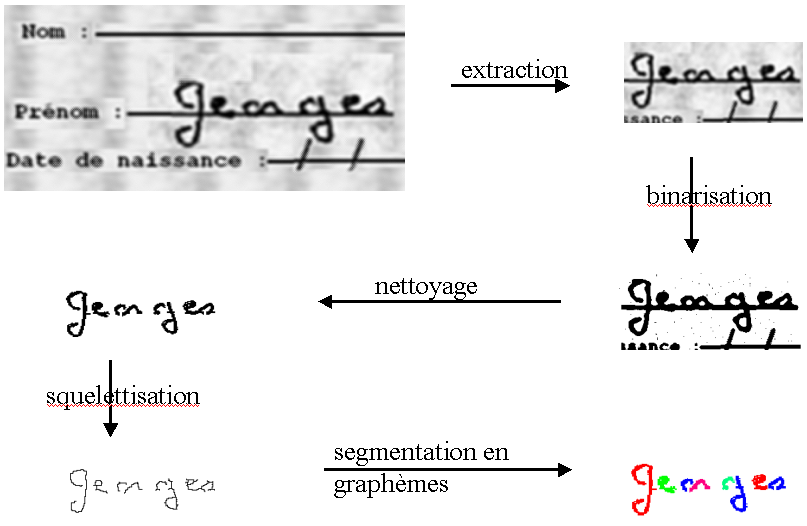
\includegraphics[height=6cm, width=10cm]
	    {\filext{../image/image/global}}\end{array}$}$$
	    \caption{Sch�ma global des pr�traitements d'image.}
	    \label{image_global}
			\end{figure}
			
\indexfr{heuristique}			
\indexfr{nettoyage}
\indexfr{graph�me}
Chacune de ces �tapes est souvent tr�s rapide et est fr�quemment bas�e sur des heuristiques. L'extraction, la binarisation, la squelettisation\seeannex{annexe_squelettisation}{squelettisation} sont des traitements communs qui ne seront pas plus d�taill�s. Le nettoyage est en pratique adapt� pour chaque type de probl�me. Le nettoyage d'un peigne est diff�rent du nettoyage d'une ligne et il n'existe pas encore de m�thode g�n�rale pour ce type de t�che. Le redressement se r�duit � l'estimation de l'inclinaison du texte, une m�thode bas�e sur des histogrammes convient comme celle expliqu�e au paragraphe~\ref{image_seg_line} ou celle du paragraphe~\ref{image_redressement_sobel}. La plupart de ces pr�traitements sont d�crits sommairement dans~\citeindex{Yanikoglu1998}.
			
L'objectif avou� de cette partie est la conception d'une segmentation en graph�mes, c'est-�-dire le d�coupage de l'image d'un mot en une succession d'images correspondant � ses lettres ou � des morceaux de ses lettres qui seront utilis�s plus tard par des mod�les de reconnaissance de l'�criture. C'est un traitement souvent complexe et rarement parfait. Segmentation et reconnaissance sont encore deux �tapes distinctes et ceci explique pourquoi ce traitement inclut g�n�ralement une multitude de cas particuliers (voir~\citeindex{Lecolinet1991}, \citeindex{Simon1992}). La figure~\ref{image_grapheme_erreur} r�sume les faiblesses d'un algorithme de segmentation en graph�mes. Ce traitement produit des erreurs quelle que soit la m�thode choisie car il est des configurations qui n�cessitent la reconnaissance des lettres � segmenter afin d'�tre tranch�es comme la lettre "m" qui se confond avec le couple "rn".
	    
	    
			\begin{figure}[t]
	    $$\frame{$\begin{array}[c]{c}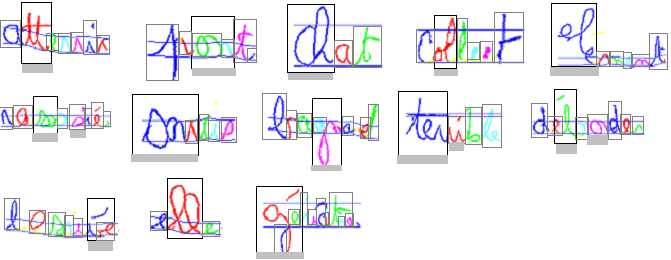
\includegraphics[height=8cm, width=16cm]
	    {\filext{../image/image/failure}}\end{array}$}$$
	    \caption{  	Erreurs de segmentation en graph�mes pour un algorithme (voir~\citeindexfig{Baret1991}) 
	    						qui s'appuie 
	    						essentiellement sur le squelette. Cette op�ration est erronn�e dans environ 10\% des cas.
	    						Comment segmenter les deux premi�res lettres du mot "souris" ou "chat" alors que, dans ces
	    						deux cas, ce sont presque deux boucles qui poss�dent une paroi commune~? Ces configurations
	    						sont difficiles � segmenter car les lettres sont souvent �crites de mani�re enchev�tr�e
	    						comme les deux "t" cons�cutifs, les lettres � liaisons hautes (b,o,v,w).}
	    \label{image_grapheme_erreur}
			\end{figure}
			
\indexfrr{liaison}{haute}			
	    						
L'algorithme utilis� pour d�couper les mots de la figure~\ref{image_grapheme_erreur} segmente mal les couples de lettres � liaison haute comme "oi" contrairement au couple "da" pour lequel, il y a tr�s peu d'erreurs. Il n'est pas �vident de juger de l'efficacit� d'un algorithme de segmentation en graph�mes, le r�sultat peut �tre d�cevant pour l'\oe il humain et n�anmoins �tre performant s'il est appari� � des mod�les de reconnaissance qui peuvent par exemple mod�liser ses erreurs (voir paragraphe~\ref{hmm_bi_lettre}, page~\pageref{hmm_bi_lettre}). 

Les paragraphes qui suivent se proposent de d�crire diff�rentes m�thodes de segmentations (lignes, mots, graph�mes) qui permettront de r�soudre le probl�me de reconnaissance de mots-cl� dans un paragraphe manuscrit. Il y aura peu d'�valuation de performances car il est difficile de juger la qualit� d'un traitement d'image autrement qu'en observant. La seule sanction est le taux de reconnaissance~: combien d'images ont-elles �t� bien d�crypt�es~? Et dans le cas d'une am�lioration des performances, on peut se demander si celles-ci sont dues � une am�lioration de la segmentation en graph�mes ou � une meilleure mod�lisation de cette derni�re par des mod�les probabilistes.

L'objectif de cette partie n'est donc pas d'am�liorer une segmentation graph�me existante (celle developp�e dans~\citeindex{Baret1991}) mais d'en proposer une autre afin d'obtenir deux cha�nes de reconnaissance suffisamment diff�rentes afin que leurs r�sultats soient si possible corr�l�s pour des images de bonne qualit� mais divergents pour des images de qualit� moyenne.







%-------------------------------------------------------------------------------------------------------------
\section{Apprentissage d'une segmentation}
%-------------------------------------------------------------------------------------------------------------
\label{image_apprentissage_segmentation}
\indexfrr{apprentissage}{segmentation}
\indexfr{Vorono�}
\indexfr{diagramme de Vorono�}
\indexfr{composante connexe}
\indexfr{connexit�}
\indexfr{squelette}

La segmentation en graph�mes pr�sent�e par la suite (paragraphe~\ref{image_choix_segmentation}) s'appuie sur de nombreux seuils fix�s "manuellement", ajust�s lors de la visualisation du r�sultat sur quelques images. Ces heuristiques interviennent lors de la segmentation d'une mani�re qui rend impossible une estimation autre qu'un t�tonnement progressif. Une segmentation pouvant �tre apprise a l'avantage de pouvoir �tre modifi�e en utilisant les r�sultats de la reconnaissance. Le second objectif vis� est une adaptation plus facile lorsque les documents � traiter changent. De plus, il serait possible d'envisager une boucle alternant les apprentissages de la reconnaissance et de la segmentation automatique. 




\subsection{Principe}


Cette id�e s'appuie sur les diagrammes de Vorono� qui proposent un maillage d'une image (figure~\ref{image_voronoi1}). L'image est d'abord d�crite par ses composantes connexes puis r�duite � l'�tat de squelette\seeannex{annexe_squelettisation}{squelettisation}. Ce squelette est ensuite d�coup� de mani�re � ce que les morceaux ainsi form�s soient coh�rents avec la segmentation d�sir�e. En r�sum�, aucun des morceaux obtenus ne doit appartenir � deux zones diff�rentes (voir~\ref{image_voronoi1}).

			\begin{figure}[ht]
	    $$\frame{$\begin{array}[c]{ccc}
	    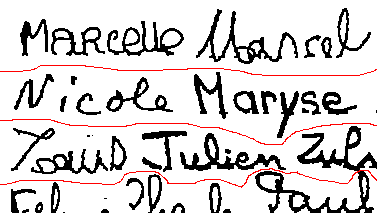
\includegraphics[height=3.5cm, width=5cm] {\filext{../image/image/voronoi0}} & & 
	    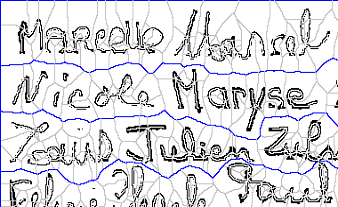
\includegraphics[height=3.5cm, width=5cm] {\filext{../image/image/voronoi1}}
	    \end{array}$}$$
	    \caption{	Diagramme de Vorono� utilis� pour une segmentation en lignes~: l'image de gauche repr�sente la 
	    					segmentation � apprendre, les lignes fonc�es de l'image de droite indiquent les fronti�res du 
	    					diagramme de Vorono� correspondant le mieux aux fronti�res entre les zones 
	    					de la segmentation d�sir�e.}
	    \label{image_voronoi1}
			\end{figure}

La segmentation en lignes d'une image telle que celle de la figure~\ref{image_voronoi1} devient un probl�me de classification en deux classes~: chaque segment du diagramme de Vorono� est une fronti�re entre deux zones � partager ou ne l'est pas. Comme le montre la figure~\ref{image_voronoi_local}, la classification d'un segment peut int�grer des informations relatives aux segments connect�s aux deux extr�mit�s ainsi que des caract�ristiques sur la forme du texte dans le voisinage de ce segment. L'objectif est la recherche d'une fonction du type~:

			\begin{eqnarray}
			f : S \times S^S_1 \times S^S_2 \times F^S_1 \times F^S_2 \longrightarrow \cro{0,1}
			\label{image_voronoi_f}
			\end{eqnarray}
		
			\begin{figure}[ht]
	    $$\frame{$\begin{array}[c]{ccc}
	    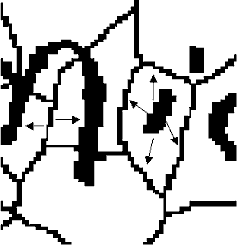
\includegraphics[height=3cm, width=3cm] {\filext{../image/image/voronoi10}} &&
	    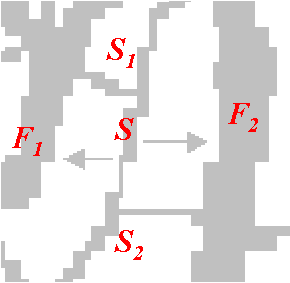
\includegraphics[height=3cm, width=3cm] {\filext{../image/image/voronoi11}}
	    \end{array}$}$$
	    \caption{	Voisinage d'un segment du diagramme de Vorono�~: tout segment 
	    					est connect� � d'autres segments � ses 
	    					deux extr�mit�s et il s�pare deux zones contenant chacune une petite partie 
	    					du texte que contient l'image.}
	    \label{image_voronoi_local}
			\end{figure}
			
$S$ est vecteur caract�risant le segment � classer, $S^S_1$ et $S^S_2$ sont deux vecteurs de m�me dimension caract�risant les vecteurs connect�s � $S$ � chacune de ses deux extr�mit�s, $F^S_1$ et $F^S_2$ sont deux vecteurs caract�risant la forme du contenu des deux zones de textes que $S$ s�pare (figure~\ref{image_voronoi_local}). 
			



\subsection{Exp�rimentations}


Dans un premier temps, la fonction $f$ (\ref{image_voronoi_f}) a �t� estim�e � l'aide d'un r�seau de neurones classifieur\seeannex{subsection_classifieur}{classifieur}. Les vecteurs $S$, $F^S_1$, $F^S_2$ contenaient des informations relatives � la longueur du segment, sa courbure, son inclinaison, la distance du segment au texte. Les vecteurs $S^S_1$ et $S^S_2$ contenaient des moyennes des m�mes informations. L'estimation de la fonction $f$ a conduit au r�sultat figure~\ref{image_voronoi2} avec un pourcentage de bonne classification proche de 95\%.

			\begin{figure}[ht]
	    $$\frame{$\begin{array}[c]{c}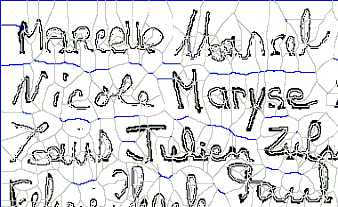
\includegraphics[height=5cm, width=7cm]
	    {\filext{../image/image/voronoi2}}\end{array}$}$$
	    \caption{	Diagramme de Vorono� utilis� pour une segmentation en lignes~: 
	    					le r�sultat laisse appara�tre des lignes
	    					en pointill�. Dans 95\% des cas, les segments de Vorono� sont bien class�s.}
	    \label{image_voronoi2}
			\end{figure}
			
M�me si le pourcentage d'erreur est faible, il m�ne � l'apparition de lignes "trou�es" qui sugg�re soit l'abandon de la m�thode, soit son perfectionnement selon deux directions qui sont la cr�ation d'un processus it�ratif permettant de faire �voluer la probabilit� d'un segment en fonction de ses voisins et un post-traitement dont l'objectif est l'�limination des "trous". La premi�re direction passe par la construction d'une suite $\pa{p_t}$ pour chaque segment de telle sorte que~:

			\begin{eqnarray*}
			p^S_0 &=& f\pa{S, S^S_1, S^S_2, F^S_1, F^S_2} \\
			\forall t \supegal 0, \; p^S_{t+1} &=& g\pa{p^S_t, S, p^{S_1}_t, S^S_1, p^{S_2}_t, S^S_2, F^S_1, F^S_2}
			\end{eqnarray*}
			
Le processus s'arr�te lorsque la suite $\pa{p^S_t}_{t\supegal 0}$ converge pour chaque segment $S$. Il reste � estimer la fonction $g$. Le nombre d'it�rations n�cessaires � la convergence d'un tel syst�me demeure inconnu. La seconde direction correspond en quelque sorte au nettoyage des r�sultats retourn�s par la fonction $f$ (ou son prolongement $g$), les lignes presque achev�es sont compl�t�es, les bouts de lignes ne menant � rien sont effac�es. 

Cette m�thode s'appuie sur un diagramme de Vorono� qui peut s'av�rer instable lorsque l'image est de mauvaise qualit�, lorsque quelques pixels �gar�s cr�ent des r�gions artificielles. Les diagrammes de Vorono� flous (\citeindex{Zhao2000}) seraient peut-�tre une alternative � ce probl�me. De plus, la convergence de l'ensemble n'est pas assur�e et peut d�boucher sur des temps de traitements longs inconvenants pour des applications telles que la reconnaissance de l'�criture. Aucun des deux prolongements n'a �t� �tudi�.
			
			





\subsection{Extension au probl�me de nettoyage}

\indexfr{nettoyage}
\indexfr{Vorono�}

Le nettoyage est un probl�me dual du pr�c�dent puisqu'au lieu de classer les segments du diagramme de Vorono�, il suffit de classer les zones d�limit�es par ce diagramme en deux classes~: zone � nettoyer ou non. L'avantage du diagramme de Vorono� est de proposer un voisinage (figure~\ref{image_voronoi_local}) pour chaque petite r�gion. Une application pratique est la suppression d'une ligne qui sert de guide pour l'�criture comme celle montr�e figure~\ref{image_global}. L'int�r�t de la m�thode r�side toujours dans son apprentissage et son inconv�nient dans la forte sensibilit� du diagramme de Vorono� aux ruptures de connexit�.







\subsection{Diagramme de Kohonen}
\indexfr{Kohonen}
\indexfr{relaxation probabiliste}
\indexfr{champs de Markov}
\indexfrr{Markov}{champs}
\indexfrr{segmentation}{ligne}
\indexfrr{segmentation}{mot}

Outre le fait que le diagramme de Vorono� est tr�s sensible au bruit, pour une r�gion donn�e, le nombre de voisins est tr�s variable, il est alors n�cessaire de r�sumer l'information contenue par ce voisinage. On utilise une carte de Kohonen dont la structure est celle d'un quadrillage. Les pixels noirs attirent les neurones qui �tirent les ar�tes qui les relient comme le montre la figure~\ref{image_koho_lines}a. Les ar�tes les plus grandes forment des ponts entre deux r�gions, un simple seuillage (figure~\ref{image_koho_lines}b) permet presque d'isoler les mots. L'avantage de cette nouvelle structure est son voisinage de taille fixe, quelle que soit la d�formation du treillis de Kohonen, chaque neurone conservera quatre voisins, il est alors possible d'utiliser des algorithmes (relaxation probabiliste, champs de Markov) permettant de classer les ar�tes en deux cat�gories~: ar�te � l'int�rieur d'une r�gion, ar�te reliant deux r�gions � segmenter.



			\begin{figure}[ht]
	    $$\begin{tabular}{|c|c|}\hline
	    \includegraphics[height=4cm, width=6cm]{\filext{../image/image/koholine1}} &
	    \includegraphics[height=4cm, width=6cm]{\filext{../image/image/koholine2}} \\
	    $(a)$ & $(b)$ 
	    \\ \hline \end{tabular}$$
	    \caption{	Treillis de Kohonen appliqu� � la segmentation en ligne, l'image $(a)$ 
	    					pr�sente le r�sultat apr�s convergence
	    					des neurones, l'image $(b)$ repr�sente le m�me treillis dont les ar�tes les 
	    					plus grandes ont �t� �t�es. Il reste dans le meilleur des cas des assemblages connexes
	    					recouvrant l'image d'un des mots.}
	    \label{image_koho_lines}
			\end{figure}


L'inconv�nient de cette m�thode r�side dans l'obtention du treillis final de Kohonen, la convergence est gourmande en temps de calcul pour de grandes images. C'est pour cela que cette id�e n'a pas �t� poursuivie. En revanche, ce temps de calcul devient acceptable si la dimension de l'image est celle d'un mot, cette m�thode pourrait donc �tre utilis�e pour apprendre une segmentation en graph�mes. 

Cet apprentissage n�cessite malgr� tout de nombreuses images pour lesquelles la segmentation en graph�mes doit �tre connue. L'obtention d'une telle base de donn�es peut �tre manuelle mais ce travail est long ou effectu� � partir d'un syst�me de reconnaissance d�j� existant mais contenant des erreurs. Les mots les mieux reconnus sont alors d�coup�s en graph�mes ou caract�res selon l'usage d�sir� puis serviront d'apprentissage. Cette direction n'a pour le moment pas �t� envisag�e, une autre permettant de mod�liser des erreurs de segmentation en graph�mes lui a �t� pr�f�r�e dans un premier temps (voir paragraphe~\ref{hmm_bi_lettre}, page~\pageref{hmm_bi_lettre}). \indexfrr{segmentation}{graph�me} \indexfr{graph�me} Cette mod�lisation permet d'ailleurs une meilleure appr�ciation de la segmentation en graph�mes.













%-------------------------------------------------------------------------------------------------------------
\section{Segmentation en lignes}
%-------------------------------------------------------------------------------------------------------------
\label{image_seg_line}
\indexfrr{segmentation}{ligne}
\indexfr{histogramme}

Lors de la scannerisation d'un document, il peut arriver que celui-ci soit inclin� (figure~\ref{image_segline_direction}). La premi�re �tape consiste donc � redresser une image de telle sorte que les lignes qui la composent soient horizontales. Ce paragraphe aborde diverses solutions existantes et r�sume les r�sultats �nonc�s dans~\citeindex{Dupr�2000}.






\subsection{Redressement de l'inclinaison de l'image}
\indexfr{inclinaison}


De nombreuses m�thodes sont utilis�es pour d�tecter l'inclinaison des lignes, leurs robustesses variant avec la difficult� du probl�me. L'article~\citeindex{Cao2003} par exemple propose une m�thode plus adapt�e aux textes imprim�s. Les composantes connexes (des lettres principalement) sont toutes d�crites par un point situ� au milieu du bord inf�rieur de leurs bo�tes englobantes. Par la suite, ces points sont regroup�s et class�s en lignes. Une r�gression lin�aire sur chacune des lignes termine l'estimation de l'inclinaison de l'image. \indexfr{cha�ne de plus proches voisins} Une autre m�thode pr�sent�e dans~\citeindex{Lu2003} utilise des cha�nes de plus proches voisins (ou nearest neighbors chains), celles-ci sont constitu�es par l'appariement de voisins. L'inclinaison est mesur�e sur chacune des cha�nes qui doivent �tre suffisamment longues pour une mesure pr�cise mais pas trop pour �viter le regroupement de voisins trop �loign�s n'appartenant pas � la m�me ligne de texte. \indexfrr{Hough}{transform�e de ...} La transform�e de Hough est aussi une m�thode tr�s utilis�e (voir~\citeindex{Pal1996}), chaque petit segment de l'image permet d'estimer les coefficients du vecteur directeur de la droite qui le soutient. La direction de l'inclinaison du document correspond aux coefficients les plus repr�sent�s. Les histogrammes permettent �galement d'estimer cette inclinaison (voir~\citeindex{Bloomberg1995}) comme de segmenter l'image redress�e en lignes (voir~\citeindex{Gatos1997}, \citeindex{Pal2001}). C'est cette approche qui est pr�sent�e ici.




			\begin{xdefinition}{histogramme}
			\indexfr{histogramme}
			
			L'histogramme d'une image selon une direction $\alpha$ est une projection de cette image 
			sur une droite parall�lement � une droite de vecteur directeur $d=\pa{\begin{subarray}{c} 1 
			\\ tan \alpha \end{subarray}}$. Concr�tement, si $I$ est une image de dimension $\pa{X,Y}$, un
			histogramme est un vecteur dont chaque �l�ment contient le nombre de pixels noirs sur une ligne de
			direction~$d$ trac�e avec un algorithme comme celui de~\citeindex{Bresenham1965} (voir
			�galement~\citeindex{Bresenham1977}).
			
			\end{xdefinition}



La qualit� de l'histogramme ou sa pertinence est estim�e par son entropie.



		\begin{xdefinition}{entropie d'un histogramme}
		\indexfr{entropie d'un histogramme}
		
		Soit $H = \vecteur{h_1}{h_n}$, on d�finit le vecteur d�fini par $H' = \vecteur{p_1}{p_n}$~:
		
					$$
					\forall i \in \intervalle{1}{n}, \; p_i =  \frac{h_i} { \summy{k=1}{n} \, h_k }
					$$
		
		L'entropie de l'histogramme $H$ est le nombre suivant calcul� sur l'histogramme $H'$~:
		
					\begin{eqnarray}
					E\pa{H} &=& E\pa{H'} = \summy{i=1}{n} \; p_i \, \ln p_i
					\end{eqnarray}
		
		\end{xdefinition}

\indexfr{redressement}\indexfr{glissement de pixels}

La direction la plus probable est celle qui maximise l'entropie (voir~\citeindex{C�t�1997}). Graphiquement, l'histogramme d'entropie maximale est celui dont les extrema sont les plus marqu�s (voir figure~\ref{image_segline_direction}).
L'image est finalement redress�e de fa�on � ce que l'image ne contienne plus des lignes horizontales. Ce redressement peut tout simplement �tre effectu� par un glissement des colonnes de pixels de l'image les unes par rapport aux autres. 


			\begin{figure}[t]
	    $$\frame{$\begin{array}[c]{c}\includegraphics[height=4cm, width=14cm]
	    {\filext{../image/image/segline1}}\end{array}$}$$
	    \caption{	Segmentation en lignes~: recherche de la meilleure orientation, celle-ci accentue 
	    					le plus possible les extrema.}
	    \label{image_segline_direction}
			\end{figure}


\indexfr{Radon}\indexfrr{transform�e}{Radon}\indexfr{Hough}\indexfrr{transform�e}{Hough}
Il existe des m�thodes plus r�centes comme par exemple celle d�crite dans \citeindex{Kapoor2004}. A partir d'une transform�e de Radon de l'image et d'une transform�e de Hough. Cette m�thode est plus souple que la pr�c�dente. La m�thode des histogrammes d�termine l'orientation la plus probable dans un ensemble discret de solutions possibles. L'article \citeindex{Kapoor2004} d�termine directement cette meilleure orientation.




\subsection{Segmentation en lignes}\label{section_segmentation_ligne}
\indexfrr{segmentation}{ligne}


L'histogramme obtenu figure~\ref{image_segline_direction} est bruit�. Afin de diminuer l'importance de ce bruit, l'histogramme est liss� par la m�thode des moyennes mobiles. Selon les probl�mes, la taille de cette moyenne est plus ou moins grande. Soit $H_l = \vecteur{l_1}{l_n}$ l'histogramme liss�, il est donc obtenu � partir de $H$ comme suit~:


			\begin{eqnarray}
			\begin{array}{rrcl}
			\forall i \in \intervalle{w+1}{n-w-1}, 	\; & 	l_i &=& \dfrac{1}{2w+1} \, \summy{k=-w}{+w} \, h_{i+k} \\
			\forall i \in \intervalle{1}{w}, 				\; & 	l_i &=& \dfrac{1}{i+w} \, \summy{k=1}{i+w} \, h_k \\
			\forall i \in \intervalle{n-w}{n}, 			\; & 	l_i &=& \dfrac{1}{n-i+ w + 1} \, \summy{k=i-w}{n} \, h_k 
			\end{array}
			\label{image_lissage_equation}
			\end{eqnarray}


Les maxima locaux indiquent la position des lignes, les minima locaux la position des fronti�res entre lignes. On d�finit pour chaque ligne les minima $\pa{m_i^x}_i$ et les maxima $\pa{M_i^x}_i$~:


			$$
			\begin{array}{rcl}
			\forall i, \; m_i^x = \left\{ \begin{array}{l}
																		1 \text{ si } l_i = \min \acc { l_k \sac l-x \infegal k \infegal l+x } \\
																		0 \text{ sinon}
																	\end{array} \right. \\
			\forall i, \; M_i^x = \left\{ \begin{array}{l}
																		1 \text{ si } l_i = \max \acc { l_k \sac l-x \infegal k \infegal l+x } \\
																		0 \text{ sinon}
																	\end{array} \right.
			\end{array}
			$$


La figure~\ref{image_segline_extrema} montre que bien souvent le nombre d'extrema d�tect�s est sup�rieur au nombre r�el d'extrema. Une �tude sur quelques dizaines d'images a permis d'�liminer les cas de mauvaises d�tections les plus courants~:

\begin{enumerate}
\indexfr{petit palier}
\item \textit{Le petit palier}~: ce cas se pr�sente le plus souvent lorsqu'une ou plusieurs majuscules font partie de la ligne de texte. Le dessin de ces lettres contient des traits horizontaux trac�s au-dessus de la ligne des minuscules. Une barre de "F" bien marqu�e peut entra�ner de mauvaises segmentations.
\indexfr{petit extremum}
\item \textit{Le petit extremum}~: lorsque les mots ne sont pas tout-�-fait bien align�s sur une m�me horizontale, les extrema sont plus diffus, il faut alors regrouper plusieurs maxima ensemble.
\end{enumerate}


Deux r�gles permettent l'�limination de ces mauvaises d�tections~:

			\begin{enumerate}
			\item Soit $\acc{e_i \sac 1 \infegal i \infegal 4}$ quatre extrema cons�cutifs, alors~:
								\begin{eqnarray}
								\abs{e_2 - e_3} \infegal \beta \abs{e_1 - e_4} \Longrightarrow 
								\acc{e_2, \, e_3} \text{ doivent �tre �limin�s.} 
								\label{image_ligne_critere_palier_1}
								\end{eqnarray}
			\item Soit $e_2$ un minimum et $e_1$ et $e_3$ les extrema qui l'entourent, alors~:
								\begin{eqnarray}
								e_2 \infegal \gamma \min\acc{e_1,e_3} \Longrightarrow 
								\acc{e_2, \, e_1 \text{ ou } e_3} \text{ doivent �tre �limin�s.} 
								\label{image_ligne_critere_palier_2}
								\end{eqnarray}
			\end{enumerate}
	
Ce processus est illustr� par la figure~\ref{image_segline_extrema}. Les valeurs int�ressantes pour les quatre param�tres $w$, $x$, $\beta$, $\gamma$ sont~:

			$$
			\begin{array}{ccccccc}
			w &=& 4  \text{ pixels} 	&&    \beta 	&=& 0,2 \\
			x &=& 4  \text{ pixels}  	&&    \gamma 	&=& 0,5 
			\end{array}
			$$



			\begin{figure}[t]
	    $$\frame{$\begin{array}[c]{c}\includegraphics[height=6cm, width=12cm]
	    {\filext{../image/image/segline2}}\end{array}$}$$
	    \caption{	Segmentation en lignes~: recherche des bons extrema. Les extrema trop proches v�rifiant les
	    					crit�res~(\ref{image_ligne_critere_palier_1}) et~(\ref{image_ligne_critere_palier_2})
	    					ne sont pas pris en compte.}
	    \label{image_segline_extrema}
			\end{figure}



Le processus de suppression des "faux" extrema n�cessite plusieurs it�rations, � chacune d'elle, le plus petit palier est isol� et supprim�, ensuite, l'op�ration est r�p�t�e pour les petits extrema. Le processus s'arr�te lorsqu'il ne peut plus rien supprimer, autrement dit, lorsqu'aucun petit palier et aucun petit extremum n'a pu �tre trouv�.





\subsection{Traitements des lignes enchev�tr�es}

\indexfrr{ligne}{enchev�tr�e}



C'est la derni�re �tape avant la reconnaissance du contenu des lignes. L'�tude de l'histogramme a permis d'encadrer chaque ligne par un rectangle dont d�passent certaines grandes lettres ascendants et/ou descendants comme les "j" ou les "p". Le module de reconnaissance des mots est bas� sur une extraction de graph�mes utilisant la connexit� du dessin des lettres.


			\begin{figure}[ht]
	    $$\frame{$\begin{array}[c]{c}\includegraphics[height=2cm, width=4cm]
	    {\filext{../image/image/segline3}}\end{array}$}$$
	    \caption{Segmentation en lignes~: connexit�}
	    \label{image_segline_connex}
			\end{figure}



En partant de la m�me id�e, on va supposer que le "j" de "Lajoie" (figure~\ref{image_segline_connex}) est form� d'une seule composante connexe. La segmentation en lignes s'ach�ve donc par le recollement des morceaux d'une m�me lettre �gar�s des deux c�t�s d'une fronti�re s�parant deux lignes. Le principe est le suivant~:

			\begin{enumerate}
			\item On parcourt la fronti�re entre deux lignes jusqu'� ce qu'on intercepte une lettre.
			\item On parcourt le contour ext�rieur du morceau situ� au-dessus, si lors de ce parcours, 
							on revient � la m�me fronti�re sans en rencontrer aucune autre, alors ce morceau de 
							lettre est consid�r� comme �tant du mauvais c�t�.
			\item On parcourt le contour ext�rieur du morceau situ� au-dessous, si lors de ce parcours, 
							on revient � la m�me fronti�re sans en rencontrer aucune autre, alors ce morceau de 
							lettre est consid�r� comme �tant du mauvais c�t�.
			\item Si un seul des deux morceaux est du mauvais c�t� alors ce morceau est remis dans la bonne ligne, 
							sinon on ne fait rien.
			\item On continue le parcours de la fronti�re au cas o� d'autres lettres intercepteraient celle-ci.
			\end{enumerate}

Dor�navant, l'extraction des lignes est termin�e. Cette m�thode fonctionne efficacement sur des adresses mais poss�de quelques �cueils r�currents (figure~\ref{image_segline_bad}).


			\begin{figure}[t]
	    $$\frame{$\begin{array}[c]{c}\includegraphics[height=12cm, width=8cm]
	    {\filext{../image/image/segline_bad}}\end{array}$}$$
	    \caption{Segmentation en lignes~: exemples qui ne marchent pas.}
	    \label{image_segline_bad}
			\end{figure}








\subsection{Segmentation � partir d'un graphe}
\indexfr{graphe}
\indexfrr{segmentation}{ligne}


L'article \citeindex{Abuhaiba1996} propose une autre alternative, une m�thode de segmentation en lignes bas�e sur un graphe $k$-connexe (voir figure~\ref{image_graphe_distance_segment_fig}). L'image d'un paragraphe est d'abord squelettis�e puis vectoris�e\seeannex{squelette_vectorisation_Abuhaiba1996}{squelettisation}. Chaque arc ainsi obtenu est ensuite reli� � $k$-plus proches voisins ordonn�s selon la distance (\ref{image_graphe_distance_segment}). Soient deux segments $S_1$ et $S_2$, la distance $d\pa{S_1,S_2}$ est d�finie par~:


			\begin{eqnarray}
			d_x\pa{S_1,S_2} 	&=&		\underset{\pa{u,v} \in S_1 \times S_2} {\min } \; \abs{ u_x - v_x } \nonumber \\
			d_y\pa{S_1,S_2} 	&=&		\underset{\pa{u,v} \in S_1 \times S_2} {\min } \; \abs{ u_y - v_y } \nonumber \\
			d\pa{S_1,S_2}			&=&		\cro { 1 + \gamma \, \pa{ \frac{\pi}{2} }^{-1}  \arctan \frac{ d_y\pa{S_1,S_2} } {d_x\pa{S_1,S_2} } }
															\; \sqrt { d_x\pa{S_1,S_2} ^2 + d_y\pa{S_1,S_2} ^ 2} 
						\label{image_graphe_distance_segment}
			\end{eqnarray}


			\begin{figure}[ht]
	    $$\frame{$\begin{array}[c]{c}\includegraphics[height=3cm, width=6cm]
	    {\filext{../image/image/abusl}}\end{array}$}$$
	    \caption{Segmentation en lignes en recherchant l'arbre de poids minimal. L'axe vertical 
	    					sur la droite de l'image est ajout� de fa�on � relier toutes les lignes entre elles, figure 
	    					extraite de \citeindexfig{Abuhaiba1996}.}
	    \label{image_graphe_distance_segment_fig}
			\end{figure}
			
\indexfr{Kruskal}
\indexfrr{arbre}{poids minimal}
			
Le param�tre $\gamma$ est choisi de telle sorte que deux segments appartenant � la m�me ligne soient plus proches que deux segments situ�s sur deux lignes cons�cutives. Chaque segment est donc reli� � ses $k$ plus proches voisins par un arc dont le poids est la distance (\ref{image_graphe_distance_segment}). A ce graphe est ajout� un axe constitu� de petits segments tr�s peu �loign�s de sorte qu'une connexion � cet axe est beaucoup moins co�teuse que tout autre connexion. L'arbre est ensuite r�duit � un arbre de poids minimal en appliquant l'algorithme de Kruskal (voir \citeindex{Kruskal1956}). La segmentation en lignes s'ach�ve par la d�tection de toutes les liaisons � l'axe virtuel non d�truit par l'algortihme de Kruskal.









%-------------------------------------------------------------------------------------------------------------
\section{Pr�traitements de l'image}
%-------------------------------------------------------------------------------------------------------------
\indexfr{pr�traitement de l'image}

Ce paragraphe regroupe ensemble diff�rents pr�traitements pr�c�dant une segmentation en graph�mes, il regroupe le redressement d'image ou l'estimation de diff�rents param�tres comme la largeur moyenne d'une lettre, son �paisseur moyenne. Contrairement � la segmentation en lignes, ces m�thodes sont particuli�res � l'�criture romaine. Les caract�res chinois par exemple pr�sentent des "imperfections" qui leur sont propres et qui n�cessitent des traitements diff�rents.




\subsection{Redressement de l'image}
\label{image_redressement_sobel}
\indexfrr{filtre}{Sobel}
\indexfr{Sobel}
\indexfr{convolution}
\indexfrr{gradient}{image}
\indexfr{inclinaison}

Une fois les lignes d'un paragraphe extraites, il est parfois utile de redresser son image lorsque le scripteur a �crit "pench�". Le rapport~\citeindex{Slavik2000} compare les performances en reconnaissance sur des images redress�es ou non et montre l'apport substantiel des m�thodes de pr�traitement d'image. Les m�thodes de redressement diff�rent bien s�r par leurs m�thodes d'estimation de l'inclinaison mais aussi par les r�gions de l'image utilis�es pour effectuer cette estimation. 

\indexfr{ascendant}
\indexfr{descendant}
L'inclinaison d'un mot est surtout visible pour les lettres poss�dant des ascendants et des descendants et c'est a priori cette partie de l'image qui doit �tre utilis�e pour l'estimation de l'inclinaison comme le sugg�re la m�thode de~\citeindex{Bozinovic1989} (voir figure~\ref{image_slant_correction_bozinovic}) qui s�lectionne les ascendants et descendants situ�s dans les parties sup�rieure et inf�rieure de l'image. 


			\begin{figure}[ht]
	    $$\begin{tabular}{|c|} \hline
	    \includegraphics[height=3cm, width=6cm]{\filext{../image/image/slantst}}  \\ \hline
	    \end{tabular}
	    $$
	    \caption{	M�thode de Bozinovic et Srihari (voir~\citeindexfig{Bozinovic1989}), figure exraite 
	    					de~\citeindexfig{Vinciarelli2000}. Le principe de cette m�thode consiste � estimer 
	    					l'orientation	du texte en ne consid�rant que les ascendants ou descendants suffisamment
	    					grands compris entre deux lignes verticales reli�es aux bords sup�rieur et inf�rieur de l'image.}
	    \label{image_slant_correction_bozinovic}
			\indexfr{ascendant}
			\indexfr{descendant}
			\end{figure}


La m�thode d�crite dans~\citeindex{Slavik2000} quant � elle mesure l'inclinaison de chaque bord lat�ral des diff�rentes composantes connexes puis en fait la moyenne pond�r�e par la longueur des segments obtenus. \citeindex{Kim1997} et \citeindex{Knerr1997} propose une estimation fond�e sur les contours. Si $n_+$ et $n_-$ d�signent le nombre de d�placements positifs et n�gatifs selon l'axe des abscisses, et $n_v$ le nombre de d�placements verticaux, l'angle~$\theta$ de l'inclinaison est obtenu � partir de l'expression de sa tangente~: $\tan \theta = \frac{n_+ - n_-}{n_v+n_++n_-}$. La m�thode de \citeindex{Vinciarelli2000} utilise des histogrammes. Pour diff�rentes valeurs d'angles $\alpha$, on calcule le nombre $H_{\alpha}\pa{x} = \frac{h_{\alpha}\pa{x}}{\Delta y_{\alpha}\pa{x}}$, o� $h_{\alpha}\pa{x}$ est le nombre de pixels sur la colonne $x$ et $\Delta y_{\alpha}\pa{x}$ la distance qui s�pare les pixels noirs situ�s le plus haut et le plus bas. $H_{\alpha}\pa{x}$ vaut $1$ uniquement si la colonne est constitu�e d'un seul segment. Ensuite, pour chaque valeur d'angle, on calcule $S\pa{\alpha} = \sum_{x, H_{\alpha}\pa{x} = 1} h_{\alpha}^2\pa{x}$. L'inclinaison du mot est alors l'angle $\alpha$ qui maximise $S\pa{\alpha}$. Toutes ces m�thodes sont mieux adapt�es � la d�tection de l'inclinaison de l'�criture romaine, d'autres types d'�criture, comme le montre l'article \citeindex{You2003} dans le cas de l'�criture cor�enne, n�cessitent des d�veloppements plus sp�cifiques. \indexfrr{�criture}{cor�enne}


La m�thode propos�e ici s'inspire de celle d�crite dans~\citeindex{Yanikoglu1998} et s'av�re plus simple que l'estimation d'histogrammes. Elle donne les m�mes r�sultats qu'une m�thode estimant l'inclinaison � partir du contour sans pour autant chercher � les obtenir. Les deux filtres de Sobel (\ref{image_eq_sobel_filtre}) (voir~\citeindex{Prewitt1970}) permettent de retrouver en chaque point de l'image la direction du gradient. 


			\begin{eqnarray}
			F_x = 
			\begin{array}{|c|c|c|} \hline
			-1 & 0 & 1 \\ \hline
			-2 & 0 & 2 \\ \hline
			-1 & 0 & 1 \\ \hline
			\end{array}
			&
			\text{ et }
			&
			F_y =
			\begin{array}{|c|c|c|} \hline
			 1 & 2 & 1 \\ \hline
			 0 & 0 & 0 \\ \hline
			-1 & -2 & -1 \\ \hline
			\end{array}
			\label{image_eq_sobel_filtre}
			\end{eqnarray}


Soit $I$ l'image d'un mot, On note $G_x = I * F_x$ et $G_y = I * F_y$ les produits de convolution de l'image par les deux filtres d�crits en (\ref{image_eq_sobel_filtre}). Il est alors possible de d�terminer en un point $\pa{x,y}$ la direction du gradient de la fa�on suivante en s'arrangeant pour que celle-ci appartienne � l'intervalle $\left[0,\pi \right[$~:

			\begin{eqnarray}
			\theta\pa{x,y} &=& \arctan\cro{\dfrac{G_y\pa{x,y}}{G_x\pa{x,y}}} 
			\in \left[0,\pi \right[
			\end{eqnarray}


Cet intervalle est ensuite divis� en $n$ sous-intervalles de longueur identique afin de construire l'histogramme $\pa{\alpha_i}_{1 \infegal i \infegal n}$ suivant~:


		\begin{eqnarray}
		\forall i \in \ensemble{1}{n}, \; \alpha_i &=&  card 
		\acc{ \pa{x,y} \in I \sac \theta\pa{x,y} \in \left[0,\pi \right[ } \nonumber
		\end{eqnarray}


			\begin{figure}[ht]
	    $$\begin{array}{|c|c|} \hline
	    \includegraphics[height=1.1cm, width=2.5cm]{\filext{../image/image/histo_word}}   &
	    \includegraphics[height=2cm, width=5cm]{\filext{../image/image/histo_incl}}   \\ \hline
	    \end{array}
	    $$
	    \caption{	R�partition de la direction du gradient pour une image de mot en neuf intervalles
	    					d'angle (les angles sont en radians).
	    					Le pic de l'histogramme est d�cal� par rapport � $\pi/2$.  }
	    \label{image_gradient_direction_histogramme}
			\end{figure}


Un exemple d'un tel histogramme est donn� par la figure~\ref{image_gradient_direction_histogramme}. Il montre un pic principal qui correspond � l'orientation des lettres hautes (t,l,...). Toutefois, � partir de quelques images, on a constat� que cet histogramme m�ne � une estimation moins pr�cise de la direction d'inclinaison qu'une moyenne sur l'ensemble des directions calcul�es en �vitant les directions proches de l'horizontale. On note $\hat{\theta}$ cette estimation~:

			\begin{eqnarray}
			\hat{\theta} &=& 		\dfrac{1}{
																\summyone{\pa{x,y}} \; 
																\indicatrice{ \theta\pa{x,y} \in \cro{\frac{\pi}{8},\frac{7\pi}{8}}} } \;
													\summyone{\pa{x,y}} \; \theta\pa{x,y} 
													\indicatrice{ \theta\pa{x,y} \in \cro{\frac{\pi}{8},\frac{7\pi}{8}}}
								\label{image_direction_estimation}
			\end{eqnarray}
			


L'image est ensuite redress�e en faisant glisser les lignes de pixels les unes sur les autres comme le montre la figure~\ref{image_gradient_direction_histogramme_correct}.


			\begin{figure}[ht]
	    $$\begin{array}{|c|c|} \hline
	    \includegraphics[height=1.1cm, width=2.5cm]{\filext{../image/image/histo_word}}   &
	    \includegraphics[height=1.1cm, width=3cm]{\filext{../image/image/histo_wori}}   \\ \hline
	    \end{array}$$
	    \caption{	Correction de l'inclinaison de l'image effectu�e par un glissement des lignes 
	    					les unes sur les autres. L'estimation de la direction par 
	    					(\ref{image_direction_estimation}) donne 58 degr�s, 90 �tant la valeur pour
	    					�criture non inclin�e.}
	    \label{image_gradient_direction_histogramme_correct}
			\end{figure}











\subsection{Lissage du contour}

\indexfrr{lissage}{contour}
\indexfrr{contour}{lissage}
\label{image_lissage_contour__}

La correction de l'inclinaison se termine par la construction de l'image corrig�e qui est le r�sultat d'un glissement des lignes de pixels les unes par rapport aux autres. Cette m�thode simple a pourtant l'inconv�nient de produire des irr�gularit�s tout le long du contour des lettres (voir figure~\ref{image_lissage_contour_said}). Ces petits bruits peuvent alt�rer les r�sultats de la reconnaissance (voir~\citeindex{Slavik2000}). 

			\begin{figure}[ht]
	    $$\begin{tabular}{|c|} \hline
	    \includegraphics[height=3cm, width=3cm]{\filext{../image/image/smoothsaid}} \\ \hline
	    \end{tabular}$$
	    \caption{	Ces deux images proviennent de la barre du "d" 
	    					de la figure~\ref{image_gradient_direction_histogramme_correct}. Le r�sultat obtenu
	    					d� aux glissements des lignes les unes par rapport aux autres 
	    					pr�sente de nombreuses irr�gularit�s qu'il serait pr�f�rable de gommer.
	    					}
	    \label{image_lissage_contour_said}
			\end{figure}

\indexfrr{point}{inflexion}

La m�thode propos�e dans~\citeindex{Slavik2000} s'appuie sur la m�me m�thode que celle qui permet d'obtenir le squelette d'une image\seeannex{annexe_squelettisation}{squelettisation}. Par l'application des masques de la figure~\ref{image_lissage_contour}, les lettres dont l'inclinaison a �t� corrig�e perdent peu � peu leurs petites rides. Le processus continue tant que l'image �volue. Cet algorithme a �t� utilis� pour lisser l'image de la figure~\ref{image_smooth_deslant} dont l'inclinaison a �t� corrig�e.
La figure~\ref{image_smooth_deslant}c montre le r�sultat obtenu gr�ce � cet algorithme de lissage utilisant les masques cit�s par la figure~\ref{image_lissage_contour}. Le r�sultat est satisfaisant, les lignes droites incluent n�anmoins de larges cr�neaux qu'il serait possible d'�laguer en �tudiant la convexit� du contour, en minimisant le nombre de ses points d'inflexion.




			\begin{figure}[t]
	    $$\begin{tabular}{|c|} \hline
	    \includegraphics[height=6cm, width=5cm]{\filext{../image/image/smoothbo}} \\ \hline
	    \end{tabular}$$
	    \caption{	Les configurations pixelliques ci-dessus permettent de lisser le contour apr�s que 
	    					l'inclinaison d'un mot a �t� corrig�e. Cette figure est extraite de \citeindexfig{Slavik2000}
	    					� laquelle il faut ajouter les configurations obtenues par rotation de celles pr�sent�es 
	    					ci-dessus.}
	    \label{image_lissage_contour}
			\end{figure}



			\begin{figure}[t]
			$$\begin{tabular}{|c|c|c|} \hline
			\includegraphics[height=3cm, width=4cm]{\filext{../image/image/imslant}} &
			\includegraphics[height=4cm, width=6cm]{\filext{../image/image/imslant_}} &
			\includegraphics[height=4cm, width=6cm]{\filext{../image/image/imslants}}  \\
			(a) & (b) & (c) \\ \hline
			\end{tabular}$$
			\caption{	L'inclinaison de l'image~(a) est corrig�e par la m�thode expos�e
								au paragraphe~\ref{image_redressement_sobel} et donne l'image~(b). Les irr�gularit�s 
								du contour sont ensuite corrig�es gr�ce � l'algorithme pr�sent� au 
								paragraphe~\ref{image_lissage_contour__} et qui aboutit � l'image~(c).}
			\label{image_smooth_deslant}
			\end{figure}
			









\subsection{Lignes d'appui}
\label{image_ligne_appui}
\indexfrr{ligne}{appui}
\indexfrr{ligne}{base}
\indexfr{ascendant}\indexfr{descendant}

Les lignes d'appui encadrent la bande des minuscules et d�limitent les zones contenant les ascendants et descendants (voir figure~\ref{image_ligne_appui_fig}). Plusieurs m�thodes permettent de d�tecter ces lignes virtuelles mais toutes n�cessitent quelques lettres afin de retourner un r�sultat fiable. Il est par exemple impossible de distinguer un "o"~minuscule d'un "O"~majuscule si aucune autre lettre qui serait juxtapos�e ne vient aider la lecture. 

\indexfrr{Hough}{transform�e de ...}
L'article \citeindex{Wang1997} propose une m�thode utilisant ces m�mes extrema locaux du contour ext�rieur de l'image d'un mot mais les lignes d'appui sont estim�es globalement sur toute l'image � partir d'une transform�e de Hough. Comme les images sont suppos�es contenir deux lignes d'appui parall�les et proches, les r�sultats sont affin�s afin d'obtenir cette configuration.

Un autre article (\citeindex{Madhvanath1999}) sugg�re que l'estimation globale de la position de ces lignes m�ne fr�quemment � un r�sultat de mauvaise qualit� surtout si les lettres ne sont pas dispos�es sur une droite ou si les minuscules pr�sentent des tailles diff�rentes. La m�thode propos�e dans cet article s'appuie sur les extrema du contour de l'image d'un mot puis regroupe localement ces points en petits segments regroupant des points proches et presque align�s. L'ensemble de ces petits segments d�finit des lignes d'appui variables tout au long du mot.

Plusieurs histogrammes peuvent �tre utilis�s, �paisseurs des traits, nombre de transitions blanc-noir, projection des points du contour, celui-ci est souvent liss� par une moyenne mobile. En r�gle g�n�rale, la ligne d'appui basse est la plus fiable. Soit un histogramme $h=\vecteur{h_1}{h_N}$, o� $h_1$ correspond au bas de l'image et $h_i$ est la moyenne des longueurs des segments blancs de la ligne $i$. L'histogramme est liss� avec une moyenne mobile analogue � (\ref{image_lissage_equation}). On d�finit $l_b$ comme la ligne d'appui basse, $l_h$ la ligne d'appui haute, $l$ la ligne correspond au maximum de l'histogramme~:

			\begin{eqnarray}
			l \in \underset{i \in \ensemble{1}{N}} { \arg \min } \; h_i
			\end{eqnarray}

On d�finit ensuite l'intervalle $\cro{l_b,l_h}$ autour de $l$ v�rifiant~:

			\begin{eqnarray}
			\forall i \in \cro{l_b,l_h}, \; h_i \infegal \alpha \, h_l
			\end{eqnarray}

Le r�sultat de la figure~\ref{image_ligne_appui_fig} est obtenu pour $\alpha = 3$ ainsi que ceux de la figure~\ref{image_ligne_appui_fig_bad}. Ces formules peuvent �tre ajust�es manuellement sur quelques images. Puisqu'elles sont bas�es sur des histogrammes, elles sont en g�n�ral robustes. De plus, un �cart de quelques pixels n'alt�re pas les r�sultats de la reconnaissance, l'essentiel est de d�finir un rep�re qui permette de positionner les lettres les unes par rapport aux autres � partir d'une origine d�finie par les lettres. La seconde ligne d'appui repr�sente en quelque sorte un facteur d'�chelle.

			\begin{figure}[ht]
	    $$\frame{$\begin{array}[c]{c}\includegraphics[height=1cm, width=4cm]
	    {\filext{../image/image/segline_appui}}\end{array}$}$$
	    \caption{	Lignes d'appui encadrant la bande des minuscules}
			\indexfrr{ligne}{appui}
	    \label{image_ligne_appui_fig}
			\end{figure}

			\begin{figure}[ht]
	    $$\frame{$\begin{array}[c]{c}\includegraphics[height=3cm, width=8cm]
	    {\filext{../image/image/seg_appui_bad}}\end{array}$}$$
	    \caption{	Mauvais positionnement des lignes d'appui~: les mots sont trop courts ou incluent 
	    					des minuscules d�cor�es comme la lettre "i". Ces cas sont minoritaires.}
			\indexfrr{ligne}{appui}
	    \label{image_ligne_appui_fig_bad}
			\end{figure}

Afin de limiter les erreurs comme celles pr�sent�es figure~\ref{image_ligne_appui_fig_bad}, les algorithmes incluent parfois une pr�classification des histogrammes en quatre classes qui d�terminent s'il faut chercher les lignes d'appui, une seule ou aucune~: (voir~\citeindex{Hennig2002})

			\begin{enumerate}
			\item mot sans ascendant, sans descendant
			\item mot avec ascendant(s), sans descendant
			\item mot sans ascendant, avec descendant(s)
			\item mot avec ascendant(s), avec descendant(s)
			\end{enumerate}

Le principe expos� ci-dessus est valable essentiellement pour des images de mots. Pour une ligne enti�re compos�e de plusieurs mots, m�me si la m�thode ci-dessus peut servir de premi�re approximation, elle doit �tre affin�e pour chacun des mots en utilisant les bo�tes englobantes des graph�mes par exemple (paragraphe~\ref{image_segmentation_grapheme}). L'article~\citeindex{Hennig2002} pr�sente une autre m�thode bas�e sur des splines r�solvant ce probl�me.





















\subsection{Estimation de l'�paisseur du trac�}
\label{image_epaisseur_trace}
\indexfr{�paisseur du trac�}

Selon les scripteurs, l'�criture peut-�tre plus ou moins �paisse (voir figure~\ref{image_trace_epaisseur}). Cette diff�rence n'est pas toujours int�ressante � prendre en compte (redressement de l'image) comme elle peut parfois �tre une donn�e non n�gligeable. Par exemple, on consid�re un histogramme de projection verticale utilis� pour la segmentation graph�me (paragraphe~\ref{image_segmentation_histogramme_direction}), ses minima locaux sont a priori sup�rieurs � l'�paisseur du trait qui peut servir de seuil de coupure.



			\begin{figure}[ht]
	    $$\begin{array}{|c|c|}\hline 
	    \includegraphics[height=1cm, width=3cm]{\filext{../image/image/attitude1}} &
	    \includegraphics[height=1cm, width=3cm]{\filext{../image/image/attitude2}} \\ \hline
	    \end{array}$$
	    \caption{	Diff�rentes �paisseurs de trac� pour deux images dont les dimensions sont 206x69 pixels 
	    					pour la premi�re et 211x97 pixels pour la seconde.}
	    \label{image_trace_epaisseur}
			\end{figure}

L'article \citeindex{Abuhaiba1996} propose une estimation � partir d'une carte de distance\seeannex{ske_carte_distance_sec}{carte de distance} et d'un masque de distance d�fini comme suit~:

			$$
			\begin{array}{c|c|c}
			4 & 3 & 4 \\ \hline
			3 & 0 & 3 \\ \hline
			4 & 3 & 4 \\
			\end{array}
			$$

On note $d_*$ la valeur de la distance la plus fr�quente, l'�paisseur du trait $\widehat{e_0}$ est alors d�finie comme~:

			\begin{eqnarray}
			\widehat{e_0} &=& \frac{2}{3} \; d^* - 1
			\end{eqnarray}



\indexfrr{histogramme}{segment}
Cette estimation peut �tre aussi effectu�e au moyen d'histogrammes de projection. Une ligne ou une colonne de pixels extraite de l'image est constitu�e d'une suite de segments de la couleur de l'�criture. A priori, la longueur minimale de ces segments est �gale � l'�paisseur du trait. Par cons�quent, on construit l'histogramme $\pa{h_i}_{1 \infegal i }$ suivant~:

			\begin{eqnarray}
			\forall i \supegal 1, \; h_i &=& card  \acc{ \text{ segments de longueur $i$ } }
			\end{eqnarray}


La figure~\ref{image_trace_epaisseur_histo} illustre les histogrammes obtenus pour les deux images de la figure~\ref{image_trace_epaisseur}. La longueur (\ref{image_epaisseur_estimateur_1}) correspondant au maximum est une premi�re estimation de l'�paisseur du trait. Un second estimateur (\ref{image_epaisseur_estimateur_2}) est construit � partir de celui-ci dans le cas o� on consid�re que la distribution de la longueur des segments suit grossi�rement une loi normale autour de cet extremum~: 

		\begin{eqnarray}
		\widehat{e_1} &=&	\underset{i \supegal 1}{\arg \max} \; h_i \label{image_epaisseur_estimateur_1} \\
		\widehat{e_2}	&=&	\frac{1}{h} \; \summy{i = 1}{2\widehat{e_1}} \; i \; h_i  
																							\label{image_epaisseur_estimateur_2} 
		\end{eqnarray}



			\begin{figure}[ht]
	    $$\begin{array}{|c|}\hline 
	    \includegraphics[height=3cm, width=6cm]{\filext{../image/image/epais}} \\ \hline
	    \end{array}$$
	    \caption{	Histogramme de r�partition des longueurs des traits pour les deux images
	    					de la figure~\ref{image_trace_epaisseur}.}
	    \label{image_trace_epaisseur_histo}
			\end{figure}




		\begin{table}[ht]
    $$\begin{array}{|c|c|c|}\hline 
    											& \text{premi�re image} & \text{seconde image} \\ \hline
  	\widehat{e_1}  				&	4											& 10 		\\ \hline
  	\widehat{\sigma\pa{\widehat{e_2}}} 		
  												&	0,15	  				& 0,20 \\ \hline
    \end{array}$$
    \caption{	Valeurs obtenues par les deux estimateurs d�finis en (\ref{image_epaisseur_estimateur_1}) 
    					et (\ref{image_epaisseur_estimateur_2}) 
    					pour les deux images de la figure~\ref{image_trace_epaisseur}.}
    \label{image_trace_epaisseur_estimateur_valeur}
		\end{table}

\indexfr{largeur moyenne d'une lettre}

Cette �paisseur est calcul�e pour les deux images de la figure~\ref{image_trace_epaisseur} dans la table~\ref{image_trace_epaisseur_estimateur_valeur}. N�cessairement, la largeur d'une lettre d�passe l'�paisseur du trait et on peut vraisemblablement penser que la largeur des lettres est au moins sup�rieure � deux fois cette �paisseur (voir~\citeindex{Yanikoglu1998}).











\subsection{Estimation de la largeur moyenne d'une lettre}
\label{image_largeur_lettre}
\indexfr{largeur moyenne d'une lettre}

La largeur d'une lettre peut �tre une information int�ressante � prendre en compte lors de la segmentation en graph�mes. Cette grandeur est d'abord estim�e par la longueur moyenne entre deux transitions pixel noir - pixel blanc dans la bande des minuscules d�limit�es par les deux lignes d'appui estim�es au paragraphe~\ref{image_ligne_appui}. Cette estimation est not�e $e_l$ par la suite.







\subsection{Nettoyage de l'image}
\indexfr{nettoyage}


Les illustrations repr�sentent souvent des images binaires o� seul le mot � reconna�tre appara�t. Toutefois, ces images "propres" sont rarement celles imm�diatement obtenues apr�s scannerisation du document. Il n'existe pas de m�thodes g�n�rales associ�es � ces nettoyages car ils d�pendent fortement du type de documents � traiter et des informations qui doivent y �tre reconnues. Les algorithmes d�velopp�s sont donc sp�cifiques � un type pr�cis de document (ch�que, ordonnance, feuille de maladie, ...). N�anmoins, il se d�gage trois cat�gories de pr�traitements~: la binarisation (voir \citeindex{Kwon2004}) ou tout traitement d'image global, la localisation ou la recherche de l'information � reconna�tre et � extraire, le nettoyage proprement dit qui consiste � enlever tout ce qui peut g�ner la reconnaissance de la partie extraite, c'est un traitement local.

\indexfr{soulignement}
\indexfr{binarisation}

La figure~\ref{image_nettoyage_texte} est un exemple emprunt� � une image en niveaux de gris dont le fond est fonc�. La premi�re �tape consiste g�n�ralement � binariser l'image. Ce premier traitement n'est pas incontournable mais il permet de r�duire fortement la taille des images lors de la constitution de grandes bases de donn�es et d'utiliser des algorithmes fond�s sur la connexit�. L'image de la figure~\ref{image_nettoyage_texte} est d�j� le r�sultat d'une extraction dont il faut ensuite enlever le trait de soulignement et les formes situ�es au-dessous du mot. Le r�sultat de ces pr�traitements correspond � la seconde image de la figure~\ref{image_nettoyage_texte}.



			\begin{figure}[ht]
	    $$\begin{array}{|c|c|}\hline 
	    \includegraphics[height=1.5cm, width=4cm]{\filext{../image/image/nettoy}} &
	    \includegraphics[height=1.5cm, width=4cm]{\filext{../image/image/nettoy2}} \\ \hline
	    \end{array}$$
	    \caption{	Un mot extrait d'une page en niveaux de gris, avant de pouvoir reconna�tre le mot, 
	    					il faut binariser l'image et extraire le mot � reconna�tre ce qui revient 
	    					� enlever le soulignement et les divers lettres ou trait situ�s en-dessous. 
	    					La seconde image est issue de la premi�re apr�s avoir �t� nettoy�e.}
	    \label{image_nettoyage_texte}
			\end{figure}

Les proc�dures de nettoyage du trait de soulignement consiste d'abord � estimer son �paisseur puis � enlever les pixels qui le composent en prenant soin de laisser les pixels communs aux lettres et au trait de soulignement. Ces derniers sont fr�quemment rep�r�s par une zone de sur-�paisseur due au chevauchement des traits.

\indexfr{histogramme}
\label{image_nettoyage_desolneux}

La d�tection des traits n'est pas non plus un probl�me simple m�me si, pour certains documents, le trait de soulignement est toujours pr�sent (�criture d'un nombre de famille sur une ligne horizontale par exemple). Il est possible d'utiliser des m�thodes � base d'histogrammes comme ceux pr�sent�s au paragraphe~\ref{image_seg_line}. Une autre m�thode int�ressante est pr�sent�e dans les articles \citeindex{Desolneux2000}, \citeindex{Desolneux2002}, \citeindex{Desolneux2003} qui propose un formalisme adapt� � la d�tection de toute figure g�om�trique simple comme un segment, un carr�, un cercle. Par exemple, un alignement de segments comme celui de la figure~\ref{image_nettoyage_texte_morel} n'est d�tect� que s'il est suffisamment isol� pour que sa pr�sence ne puisse pas �tre consid�r�e comme une co�ncidence. En r�sum�, � partir des segments pr�sents dans l'image, on quantifie d'abord la probabilit� d'obtenir un alignement quelconque de petits segments n'importe o� dans l'image ou plut�t le nombre moyen de segments faisant partie d'un alignement. S'il existe un ensemble de segments align�s sup�rieur au seuil d�termin� juste avant, alors, on consid�re que cet alignement est plus que probable. 


			\begin{figure}[ht]
	    $$\begin{array}{|c|}\hline 
	    \includegraphics[height=3cm, width=6cm]{\filext{../image/image/desol}}  \\ \hline
	    \end{array}$$
	    \caption{	Figure extraite de \citeindexfig{Desolneux2002}, les traits isol�s pr�sents
	    					au bas de la figure paraissent align�s mais noy�s dans le nuage au-dessus, ils 
	    					deviennent "invisibles".}
	    \label{image_nettoyage_texte_morel}
			\end{figure}

\indexfr{squelettisation}
Une m�thode plus �labor�e d�crite dans \citeindex{Cheng2004} permet de d�barrasser l'image de mots manuscrits d'une ligne ou d'une courbe sur laquelle les lettres s'appuient, ou une courbe qui traverse l'image comme celle de l'exemple de la figure~\ref{image_nettoyage_ligne_courbe}. Cette m�thode s'appuie sur la construction d'un graphe qui r�sulte d'une squelettisation. La courbe principale d�coule d'une ou plusieurs recherche d'un plus court chemin.


			\begin{figure}[ht]
	    $$\begin{array}{|c|}\hline 
	    \includegraphics[height=5cm, width=8cm]{\filext{../image/image/cheng}}  \\ \hline
	    \end{array}$$
	    \caption{	Figure extraite de \citeindexfig{Cheng2004}, la premi�re image $(a)$ est l'image originale,
	    					les deux images suivantes r�sultent du nettoyage de cette premi�re image, la courbe principale
	    					et les mots ont �t� s�par�es.}
	    \label{image_nettoyage_ligne_courbe}
			\end{figure}



%-------------------------------------------------------------------------------------------------------------
\section{Diverses segmentations en graph�mes}
%-------------------------------------------------------------------------------------------------------------
\indexfrr{segmentation}{graph�me}
\indexfr{graph�me}
\label{image_segmentation_grapheme}


La segmentation en graph�mes permet de d�localiser le probl�me de reconnaissance du niveau des mots au niveau des lettres. Reconna�tre l'image d'un mot sans la d�couper au pr�alable est une m�thode limit�e � des probl�mes restreints o� le nombre de mots est faible comme l'�criture d'un nombre en lettres. Comme la reconnaissance se r�sume � un probl�me de classification. Plus la liste des mots possibles est longue, plus le classifieur � construire est complexe. C'est pourquoi il est pr�f�rable de scinder ce probl�me de reconnaissance d'un mot en une somme de probl�mes plus simples qui sont la reconaissance des lettres pr�sentes dans l'image. 

\indexfr{MMC}\indexfrr{s�quence}{observation}
D�couper l'image soul�ve plusieurs questions dont la premi�re concerne le r�sultat � obtenir~: est-il d�pendant des mod�les de reconnaissance utilis�s par la suite~? Dans le cas de mod�les de Markov cach�s, le r�sultat souhait� est une s�quence d'observations, ce qui signifie que la seule dimension variable du d�coupage est le nombre d'objets ainsi form�s. Une extension de ces mod�les statistiques permet d'�tendre le concept de s�quence � un graphe d'observations incluant plusieurs options de segmentations. Toutefois, quelle que soit l'option choisie, elle r�sulte des compromis suivants~: 

			\begin{enumerate}
			\item Plus la segmentation poss�de de degr�s de libert� (plus elle propose d'alternatives), 
						plus les mod�les de reconnaissance seront complexes, plus les mod�les de reconnaissance 
						sont complexes, plus ils sont difficiles � apprendre.
			\item Moins la segmentation poss�de de degr�s de libert�, plus elle est susceptible de faire des erreurs.
			\end{enumerate}


Nous allons aborder une segmentation sous forme de s�quences de graph�mes. Cette �tape de segmentation est indispensable pour la construction d'un syst�me de reconnaissance de l'�criture, diverses m�thodes sont pass�es en revue dans les articles \citeindex{Lecolinet1991} ou plus r�cemment \citeindex{Lu1996}. Les paragraphes qui suivent reprennent quelques-unes des m�thodes pr�sent�es dans ces articles puis concluent sur la conception de la segmentation qui a �t� �labor�e dans le cadre de ces travaux de recherche. \indexfrr{accent}{graph�me}\indexfrr{graph�me}{accent} Cette segmentation propose �galement une solution au probl�me des accents dont la lettre d'attache est parfois situ�e assez loin, ce qui n'a pas �t� pris en compte jusqu'� pr�sent.
















\subsection{Segmentation � partir du squelette}
\indexfrr{segmentation}{graph�me}
\label{image_sequence_graphem}


\indexfr{ordonnancement}
\indexfrr{graph�me}{taille}
\indexfrr{graph�me}{ordonnancement}

Les graph�mes sont des images extraites de l'image � segmenter. Passer d'une seule image � une s�quence de graph�mes soul�ve deux probl�mes (voir~\citeindex{Baret1991}) qui sont la taille que doivent avoir les graph�mes et l'ordonnancement des morceaux segment�s. Ils ne doivent pas �tre trop petits afin d'�tre diff�rents les uns des autres, diff�rents d'un simple trait. Ils ne doivent pas �tre trop gros pour ne pas d�passer la taille d'une lettre. Chaque lettre repr�sentera entre un et trois graph�mes. Ce choix facilite l'ordonnancement des graph�mes qui doivent respecter le sens gauche-droite de la lecture. 


\indexfr{squelette}\indexfr{motifs}
L'image peut �tre rendue � l'�tat de squelette\seeannex{annexe_squelettisation}{squelettisation}. Ce dernier est ensuite parcouru de mani�re � rep�rer certains motifs synonymes de c�sure entre lettres (figure~\ref{image_graphe_cut}). La d�tection de ces motifs introduit des calculs de courbure, d'angle qui sont compar�s � des seuils ajust�s de mani�re � obtenir le r�sultat d�sir�. Ces algorithmes sont mieux d�taill�s dans~\citeindex{Lecolinet1991}.

			\begin{figure}[ht]
	    $$\frame{$\begin{array}[c]{c}\includegraphics[height=3cm, width=10cm]
	    {\filext{../image/image/grm_cut}}\end{array}$}$$
	    \caption{Segmentation � partir du squelette~: segmentation bas�e sur des motifs.}
	    \label{image_graphe_cut}
			\end{figure}

La figure~\ref{image_graphe_noel} est un exemple de ce qui est obtenu et des probl�mes qui accompagnent l'utilisation de seuils. Les lettres en fin de mots, plus petites, sont parfois agr�g�es. La figure~\ref{image_grapheme_erreur} recense la liste de ces probl�mes.

			\begin{figure}[ht]
	    $$\frame{$\begin{array}[c]{c}\includegraphics[height=1.5cm, width=5cm]
	    {\filext{../image/image/grm_noel}}\end{array}$}$$
	    \caption{	Segmentation � partir du squelette~: 
	    					chaque graph�me est entour� de sa bo�te englobante, les deux lignes horizontales
	    					mod�lisent les lignes d'appui (ou lignes de bases) qui encadrent la bande o� 
	    					sont �crites les lettres
	    					minuscules (paragraphe~\ref{image_ligne_appui}).}
	    \label{image_graphe_noel}
			\end{figure}







\subsection{Segmentation � partir du contour}
\indexfrr{segmentation}{graph�me}
\label{image_sequence_graphem_contour}
\indexfr{contour}


Cette m�thode esquiss�e dans~\citeindex{Madhvanath2001} ne s'int�resse pas au squelette mais uniquement au contour dont elle d�termine les meilleurs points candidats � une coupure entre graph�mes (voir figure~\ref{image_segmentation_contour}). Lors du parcours du contour, les extrema locaux sont marqu�s (point culminant et selle) puis les paires les plus proches sont regroup�es de part et d'autre du trait.


			\begin{figure}[ht]
	    $$\frame{$\begin{array}[c]{c}\includegraphics[height=2cm, width=4cm]
	    {\filext{../image/image/grm_seg_bound}}\end{array}$}$$
	    \caption{	Segmentation � partir du contour~: les points repr�sentent les minima et les maxima
	    					locaux (ordonn�e des points) le long du contour. Les paires des points des plus
	    					proches dispos�s de part et d'autre du trait
	    					forment les candidats les plus probables pour une c�sure.
	    					}
			\indexfrr{ligne}{appui}
	    \label{image_segmentation_contour}
			\end{figure}


\indexfr{t�tonnement}
La direction de coupure n'est pas toujours horizontale comme le montre la figure~\ref{image_segmentation_contour2}. A l'instar de la m�thode pr�c�dente, la segmentation en graph�mes � partir du contour n�cessite de nombreux ajustements avant de trouver les crit�res de d�cision. Cette mise au point par t�tonnements est le point commun de nombreux traitements d'images li�es � l'�criture manuscrite. Faciles � ajuster lorsque la qualit� de l'�criture est bonne (figure~\ref{image_segmentation_contour}), ces pr�traitements peuvent avoir des comportements tout-�-fait erratiques lorsque l'�criture est de mauvaise qualit� (voir figure~\ref{image_graphe_grapheme}).


			\begin{figure}[ht]
	    $$\frame{$\begin{array}[c]{c}\includegraphics[height=2cm, width=4cm]
	    {\filext{../image/image/grm_seg_bound2}}\end{array}$}$$
	    \caption{	Segmentation � partir du contour~: si la c�sure du couple "Je" s'appuie sur les extrema 
	    					environnants, sa direction est plus horizontale que verticale.}
	    \label{image_segmentation_contour2}
			\end{figure}







			
			
\subsection{Ordonnancement}
\indexfrr{graph�me}{ordonnancement}
\indexfr{ordonnancement}
\indexfrr{graph�me}{s�quence}
\indexfrr{s�quence}{graph�me}
\label{image_ordonnancement}
\indexfr{voyageur de commerce}

Une fois la segmentation effectu�e, il ne reste plus qu'� ordonner les morceaux afin de former une s�quence d'observations. Ce probl�me n'est pas simple et doit inclure des �tapes de regroupement afin de traiter des probl�mes tels que des accents qui doivent �tre associ�s � une lettre. Dans un premier temps, les accents, les points, c'est-�-dire tout morceau isol� au-dessus de la ligne d'appui haute, ne sont pas int�gr�s par l'algorithme d'ordonnancement, ils sont affect�s aux graph�mes une fois ce dernier termin�. Ce probl�me d'ordonnancement est similaire au probl�me du voyageur de commerce. Une fois que les graph�mes de d�but et de fin sont d�termin�s, le plus court chemin reliant les graph�mes de d�but et de fin et incluant tous les autres graph�mes peut �tre assimil� � la s�quence la plus probable.








\subsection{Fen�tres glissantes}
\indexfrr{fen�tre}{glissante}
\label{image_fenetre_glissante}

D�couper l'image en bandelettes verticales est la segmentation la plus simple comme le montre la figure~\ref{image_window_slide}. Ce d�coupage peut �tre r�gulier ou d�pendre des minima d'un histogramme de projection par exemple, il peut �galement se recouvrir. L'inconv�nient de cette m�thode est qu'elle g�n�re trop de graph�mes regroupant les morceaux de plusieurs lettres, c'est d'ailleurs pourquoi les petites images obtenues se recouvrent en partie. Le paragraphe suivant~\ref{image_segmentation_histogramme_direction} �tend cette m�thode � plusieurs directions de projection pour les histogrammes. Cette repr�sentation est utilis�e par le syst�me de reconnaissance d�crit dans \citeindex{Knerr2001}.


    \begin{figure}[t]
    $$\frame{$\begin{array}[c]{c}\includegraphics[height=2cm, width=16cm]
     {\filext{../bibliographie/image/biblio_window_slide}}\end{array}$}$$
    \caption{	Image extraite de~\citeindexfig{Knerr2001} illustrant le d�coupage de l'image d'un mot 
    					par des fen�tres glissantes.}
    \label{image_window_slide}
    \end{figure}

\indexfr{connexit�}\indexfr{ordonnancement}
Cette m�thode comme la suivante d'ailleurs poss�de n�anmoins l'avantage par rapport � celle pr�sent�e dans les paragraphes~\ref{image_sequence_graphem} et~\ref{image_sequence_graphem_contour} de n'�tre pas d�pendante de la connexit� et d'�tre moins sensible au bruit. L'ordonnancement (voir paragraphe~\ref{image_ordonnancement}) est lui aussi �vident puisque la segmentation bas�e sur le squelette ou le contour produit des morceaux r�partis dans un espace en deux dimensions alors que cette m�thode segmente l'image selon l'axe des abscisses qui est aussi l'axe de lecture.







\subsection{Segmentation bas�e sur des histogrammes}
\indexfrr{segmentation}{histogramme}
\label{image_segmentation_histogramme_direction}
\indexfr{connexit�}
\indexfr{ordonnancement}


Cette m�thode est d�crite dans l'article~\citeindex{Yanikoglu1998} et produit une segmentation semblable � celle illustr�e figure~\ref{image_grapheme_segmentation_histogramme}. Elle consiste � d�terminer des droites de segmentation de l'image � partir d'histogrammes de projection effectu�s selon diff�rentes directions proches de la verticale. Ces droites sont choisies de telle sorte qu'elles interceptent le moins de pixels noirs et sont r�guli�rement espac�es dans l'image. Cette m�thode simple et peu d�pendante de la connexit� ne peut malgr� tout pas tout r�soudre comme en t�moignent les exemples de la figure~\ref{image_grapheme_segmentation_histogramme_bad}. La m�thode poss�de �galement l'avantage de ne pas �tre assujettie au probl�me d'ordonnancement (voir paragraphe~\ref{image_ordonnancement}).




			\begin{figure}[ht]
	    $$\frame{$\begin{array}[c]{c}\includegraphics[height=1cm, width=4cm]
	    {\filext{../image/image/seg_dir_gra}}\end{array}$}$$
	    \caption{	Segmentation en graph�mes � partir d'histogrammes de projection selon
	    					plusieurs directions.}
	    \label{image_grapheme_segmentation_histogramme}
			\end{figure}



			\begin{figure}[ht]
	    $$\begin{array}{|c|c|c|} \hline
	    \includegraphics[height=1cm, width=4cm]		{\filext{../image/image/histo_seg1}} &
	    \includegraphics[height=1cm, width=2.5cm]	{\filext{../image/image/histo_seg2}} &
	    \includegraphics[height=1cm, width=2.5cm]	{\filext{../image/image/lahs_black}} \\ \hline
	    \end{array}$$
	    \caption{	Deux exemples o� la segmentation par histogramme est difficilement applicable~:
	    					le premier cas contient une barre de "t" qui sera n�cessairement coup�e puisqu'elle 
	    					touche la lettre "a". Le second exemple contient le couple "op" fortement
	    					li� du fait de l'�paisseur du trait, la liaison entre les 
	    					deux lettres est plus �paisse qu'ailleurs. Le dernier mot pr�sente un couple
	    					"La" qu'aucune droite ne saurait s�parer.}
	    \label{image_grapheme_segmentation_histogramme_bad}
			\end{figure}








\subsection{Segmentation bas�e sur des r�servoirs}
\indexfrr{segmentation}{r�servoir}
\label{image_segmentation_reservoir}
\indexfr{r�servoir}


Cette id�e est d�velop�e dans l'article~\citeindex{Pal2003} et est appliqu�e dans le cadre d'une segmentation de chiffres cursifs. Elle consiste � d�tecter tout d'abord les vall�es et les collines s�parant deux chiffres appartenant � la m�me composante connexe, ces formes sont illustr�es pour un mot dans la figure~\ref{image_grapheme_reservoir}. Deux chiffres li�s dans une m�me composante seront s�par�s si une vall�e ou une colline repr�sente un espace suffisamment grand par rapport � la taille des chiffres. En ce qui concerne les lettres, les r�gles de d�cision sont plus difficiles � mettre en place car les lettres ont des hauteurs variables.


			\begin{figure}[ht]
	    $$\begin{tabular}{|c|}\hline
	    \includegraphics[height=2cm, width=4cm]{\filext{../image/image/reser}}
	    \\ \hline \end{tabular}$$
	    \caption{	Segmentation � partir de r�servoirs d'eau (\citeindexfig{Pal2003})~: 
	    					les vall�es et les collines sont en quelque sorte	remplies d'eau, si elles
	    					sont suffisamment profondes ou hautes, elles marquent la s�paration entre deux
	    					caract�res.}
	    \label{image_grapheme_reservoir}
	    \indexfrr{r�servoir}{eau}
			\end{figure}

Une fois que les zones de coupures sont d�tect�es, il reste � d�terminer � quelle cat�gorie elle appartient (voir figure~\ref{image_grapheme_reservoir_cut}) afin de placer la c�sure � l'endroit le plus appropri�. Cette id�e est reprise dans~\citeindex{Elnagar2003} � ceci pr�s que la m�thode s'applique au squelette des chiffres et pas � l'image initiale.




			\begin{figure}[ht]
	    $$\begin{tabular}{|c|}\hline
	    \includegraphics[height=2cm, width=4cm]{\filext{../image/image/grmcut1}}
	    \\ \hline \end{tabular}$$
	    \caption{	Segmentation � partir de r�servoirs d'eau (\citeindexfig{Pal2003})~: deux points de coupures
	    					diff�rents, le premier est situ� au fond d'une vall�e � droite sur un embranchement,
	    					le second est situ� dans un creux, au milieu d'une courbe en "u". La coupure ne doit donc pas
	    					toujours intervenir � l'endroit du minimum local.}
	    \label{image_grapheme_reservoir_cut}
			\end{figure}











\subsection{Graphes de graph�mes}
\indexfrr{graphe}{graph�me}
\indexfrr{graph�me}{graphe}


La segmentation en graph�mes donne parfois des r�sultats erron�s. La figure~\ref{image_graphe_grapheme} propose une mani�re d'�viter ces erreurs en r�sumant au travers d'un graphe plusieurs options de segmentation. La s�quence de graph�mes est un cas particulier de ce graphe, elle est la segmentation la plus probable pour la partie qui concerne le traitement d'image mais pas forc�ment la meilleure pour la partie reconnaissance qui suit. Il peut donc �tre int�ressant de proposer plusieurs segmentations afin d'augmenter la probabilit� que la bonne segmentation soit trouv�e. Ce proc�d� revient souvent comme un leitmotiv dans la reconnaissance de l'�criture, il s'agit de retarder la prise de d�cision afin de conserver � chaque �tape le plus de solutions possibles.




			\begin{figure}[t]
	    $$\frame{$\begin{array}[c]{c}\includegraphics[height=7.5cm, width=12cm]
	    {\filext{../hmm_seq/image/graphe_obs}}\end{array}$}$$
	    \caption{	Segmentation en graph�mes~: graphes. Aucune d�cision n'est prise � ce niveau, 
	    					le choix de la bonne segmentation sera effectu� par le module de reconnaissance.}
	    \label{image_graphe_grapheme}
			\end{figure}






%-------------------------------------------------------------------------------------------------------------
\section{Choix d'une segmentation en graph�mes}
%-------------------------------------------------------------------------------------------------------------
\indexfrr{segmentation}{graph�me}
\label{image_choix_segmentation}


La segmentation d�crite dans les paragraphes qui suivent fonctionne bien lorsque l'�criture est de bonne qualit�. Comme tous les algorithmes de segmentation fond�s sur des heuristiques, celui-ci ne peut traiter correctement la totalit� des images. Cependant sa construction met en lumi�re les difficult�s rencontr�es lorsque la qualit� de l'�criture d�cro�t et les ajustements rendus n�cessaires par des probl�mes r�currents.



\subsection{Segmentation � partir d'histogrammes}


Le choix d'une segmentation d�pend des mod�les de reconnaissance qui devront l'utiliser. Segmenter en lettres ou morceaux de lettres les mots illustr�s par la figure~\ref{image_grapheme_segmentation_histogramme_bad} ou~\ref{image_graphe_grapheme_ing} peut para�tre une gageure. Toutefois le paragraphe~\ref{hmm_bi_lettre} permet d'assouplir cette contrainte. La segmentation propos�e ici vise seulement le d�coupage d'un mot en morceaux pouvant aller d'une simple partie de lettre � des groupes de deux ou trois lettres, pourvu que ceux-ci soient ais�ment identifiables. L'objectif est aussi d'�viter le plus possible les traitements bas�s sur la connexit� car ils sont tr�s sensibles au bruit.


			\begin{figure}[ht]
	    $$\frame{$\begin{array}[c]{c}\includegraphics[height=1cm, width=2cm]
	    {\filext{../image/image/being}}\end{array}$}$$
	    \caption{	Segmentation en graph�me d'un mot couramment employ� en langue anglaise~: \textit{being}.
	    					Les trois derni�res lettres "ing" sont simplement esquiss�es.}
	    \label{image_graphe_grapheme_ing}
			\end{figure}


L'impossibilit� de qualifier la pertinence d'une segmentation demeure un inconv�nient majeur, il est en effet difficile d'appr�cier directement un pr�traitement de l'image dont on attend les b�n�fices seulement en fin de cha�ne, c'est-�-dire en terme de taux de reconnaissance. L'appr�ciation n'est donc que visuelle.

\indexfrr{segmentation}{contour}
\indexfrr{segmentation}{squelette}
\indexfrr{segmentation}{histogramme}

L'approche propos�e ici est un compromis. La premi�re �tape consiste � segmenter gr�ce � la m�thode des histogrammes (paragraphe~\ref{image_segmentation_histogramme_direction}) en ne conservant que des coupures �videntes. Un premier ensemble de points de coupures est ainsi obtenu parmi lesquels seront s�lectionn�s ceux d�finissant la segmentation en graph�mes finale. Ce dernier r�sultat n'est pourtant pas encore parfait, ce que tenteront de corriger les m�thodes bas�es sur les contours ou les r�servoirs, celles-ci permettront ensuite de couper les morceaux litigieux.

Tout d'abord, les pixels sont projet�s selon sept directions entourant la direction verticale $-30^o$, $-20^o$, $-10^o$, $0^o$, $10^o$, $20^o$, $30^o$.  On note $\pa{h_{ij}} _ { \begin{subarray}{c} -3 \infegal i \infegal 3 \\ 1 \infegal j \infegal X \end{subarray} }$ les sept histogrammes obtenus o� $X$ est la longueur de l'image. $h_{ij}$ est donc le nombre de pixels noirs (�crits) selon une droite formant un angle $i \times 10^o$ avec la verticale et interceptant la ligne d'appui basse au point d'abscisse $j$. Ces histogrammes sont ensuite liss�s par une moyenne mobile analogue aux formules~(\ref{image_lissage_equation}). On d�finit $e_t$ comme �tant l'�paisseur du trac� (paragraphe~\ref{image_epaisseur_trace}), $e_l$ correspond � la largeur moyenne d'une lettre estim�e au paragraphe~\ref{image_largeur_lettre}. Enfin $C$ est l'ensemble de coupures et d�fini par~:


			\begin{eqnarray}
			C &=&  \acc{ h_{ij} \sac h_{ij} \infegal \beta \, e_t } \text{ o� } \beta \supegal 1
			\label{image_graphem_seg_eq_1}
			\end{eqnarray}


Le param�tre $\beta$ est g�n�ralement compris entre $1$ et $2$ de mani�re � ne pas couper un mot selon une droite interceptant deux fois le trac�. Il est possible d'�crire l'ensemble $C$ comme une r�union d'intervalles.


			\begin{eqnarray}
			C &=& \union{k=-3}{3} \union{i=1}{I} \; \cro{a_i^k, b_i^k} 
											\text{ avec } \left\{ \begin{array}{l}
																a_i^k \infegal b_i^k < a^k_{i+1} \; \forall i,k \\
																h_x^k \infegal \beta \, e_t \; \forall x \in \cro{a_i^k, b_i^k}
																\end{array} \right.
			\label{image_graphem_seg_eq_2}
			\end{eqnarray}



Pour chaque intervalle de la forme $\cro{a_i^k, b_i^k}$, on v�rifie que $b_i^k - a_i^k \infegal e_l$. Dans le cas contraire, on scinde cet intervalle jusqu'� ce que chacun des morceaux soit inf�rieur � $e_l$. La figure~\ref{image_graphem_zone_coupure_soulignement} soul�ve le probl�me de soulignement. Etant donn� la condition exprim�e en~(\ref{image_graphem_seg_eq_2}), il est impossible de s�lectionner une seule zone de coupure probable entre graph�mes. Par cons�quent, la solution adopt�e est l'introduction de points de coupure entre les zones de non-coupure correspondant � des minima locaux. 

			\begin{figure}[ht]
	    $$\frame{$\begin{array}[c]{c}\includegraphics[height=1.6cm, width=3cm]
	    {\filext{../image/image/souligne}}\end{array}$}$$
	    \caption{	S�lection des zones de coupures entre graph�mes~: probl�me des mots soulign�s,
	    					l'histogramme repr�sent� correspond � une projection verticale liss�e par une 
	    					moyenne mobile uniforme d'ordre trois.}
	    \label{image_graphem_zone_coupure_soulignement}
	    \indexfr{soulignement}
			\end{figure}
			
Dans ce cas, pour une direction donn�e $k$, l'ensemble des points de coupures correspond aux minima locaux de l'histogramme $\pa{h_i^k}_i$. Un minimum $m^k$ local v�rifie la condition suivante~:

			\begin{eqnarray}
			h^k_{m^k} &=& \min \acc{ h_x^k \sac  m^k - e_t \infegal x \infegal m^k + e_t } 
			\label{image_graphem_seg_eq_2_prime}
			\end{eqnarray}


Ces minima locaux n'existent pas toujours, dans ces cas, on cherche � d�terminer le point $c_i^k \in \cro{a_i^k, b_i^k}$, l'unique point de coupure de la zone de coupure $\cro{a_i^k, b_i^k}$. La figure~\ref{image_grapheme_reservoir_cut} sugg�re que ce point se situe � droite du milieu de cet intervalle, par cons�quent, $\tau_2 > \tau_4 > \tau_3$ dans la d�finition suivante~:

			\begin{eqnarray}
			m_i^k	&=&					\frac{a_i^k + b_i^k}{2} \nonumber \\
			c^k_i &=& 		  	\underset{x \in \pa{a_i^k, b_i^k}}{\arg \min} \; \cro {
												\tau_1 	\, \frac{h_x^k}{e_t}  + 
												\frac{4}{e_l^2}	\cro{ \indicatrice{x < m_i^k} 
																								\pa{\tau_2 - \tau_3} + \tau_3}  \;
														  						\cro{x - m_i^k}^2  +
												\frac{2 \tau_4 \; e_t^2}{e_t^2 + \abs{s_{x^-}^k - s_{x^+}^k} }
												}
			\label{image_graphem_seg_eq_3}
			\end{eqnarray}
			

\indexfrr{droite}{coupure}
\indexfrr{ligne}{appui}


			\begin{figure}[ht]
	    $$\frame{$\begin{array}[c]{c}\includegraphics[height=2cm, width=2cm]
	    {\filext{../image/image/cutcut}}\end{array}$}$$
	    \caption{	D�finition des nombres $s_{x^-}^k$ et $s_{x^+}^k$ de la 
	    					formule~(\ref{image_graphem_seg_eq_3}). $s_{x^-}^k$ correspond au nombre de pixels contenus
	    					dans la premi�re colonne du rectangle quadrill� (couleur gris fonc�), $s_{x^+}^k$ correspond
	    					� la colonne de droite (couleur noire). Le c�t� des petits carr�s est �gal � $e_t$ soit
	    					l'�paisseur moyenne de l'�criture.
	    					}
	    \label{image_graphem_aire_cut}
			\end{figure}



Les nombres $s_{x^-}^k$ et $s_{x^+}^k$ sont d�finis par la figure~\ref{image_graphem_aire_cut}. L'ensemble $\acc{c^k_i}_{ik}$ est l'ensemble des droites de segmentation possibles s�lectionn�es par l'algorithme, cet ensemble est tri� par $i$ et $k$ croissant ($i$ d'abord, l'indice $k$ d�partageant les points de m�me indice $i$) et aboutit � la suite $\pa{d_n}_{ 1 \infegal n \infegal N }$. Il reste � d�terminer quelles sont parmi les points de cette suite les droites de segmentation les plus pertinentes.


A cette suite, sont ajout�s les �l�ments s�lectionn�s par l'�quation~(\ref{image_graphem_seg_eq_2_prime}) et deux �l�ments $d_0$ et $d_{N+1}$ qui correspondent aux deux s�parations verticales de d�but et de fin, c'est-�-dire les limites de l'image. On suppose qu'il existe une distance entre deux droites de coupures $i$ et $j$ not�e $\pa{D_{ij}}_{ 0 \infegal i,j \infegal N+1 }$, trouver la meilleure segmentation revient alors � trouver le plus court chemin entre les n\oe uds $d_0$ et $d_{N+1}$ en passant ou non par $n$ autres n\oe uds $\pa{d_n}_{ 1 \infegal n \infegal N }$. Ce probl�me est usuel et r�solu par un algorithme du plus court chemin de type Djikstra (voir \citeindex{Dijkstra1971}). Il reste � d�terminer la distance $D_{ij}$ entre deux droites de coupures qui doit prendre en compte trois �l�ments~:

		\indexfr{Djikstra}
		\indexfr{plus court chemin}
		\indexfr{droite de coupure!distance@distance}

		\begin{enumerate}
		\item Le nombre de pixels noirs intercept�s par les droites de coupures, not� $p_i$ et $p_j$.
		\item Le fait que les droites s'interceptent ou non, not� $t_{ij} \in \acc{0,1}$ 
						(voir figure~\ref{image_droite_coupure_croisees}).
		\item La distance entre les deux points d'intersection des deux droites avec la ligne d'appui basse, 
						not�e $d_j - d_i$ cette distance devrait �tre proche de 
						$\lambda_4$ fois la largeur suppos�e d'une lettre, not�e $e_l$ et calcul�e au 
						paragraphe~\ref{image_largeur_lettre}.
		\end{enumerate}
		


			\begin{figure}[ht]
	    $$\frame{$\begin{array}[c]{c}\includegraphics[height=1cm, width=2cm]
	    {\filext{../image/image/droit_sec}}\end{array}$}$$
	    \caption{	Droites de coupures s�cantes issues d'une segmentation non pertinente, 
	    					deux droites de coupures peuvent se croiser, auquel cas, 
	    					il n'est pas tr�s pertinent de les associer ensemble pour former la segmentation en graph�mes. }
	    \label{image_droite_coupure_croisees}
			\end{figure}

A chaque abcisse $d_i$ est associ� un angle $u_i$ qui correspond � la direction de l'histogramme qui a permis d'obtenir $d_i$. A l'aide de ces notations, la distance $D_{ij}$ est d�finie par~:

			\begin{eqnarray}
			D_{ij} &=& 			\lambda_1 \frac{p_i + p_j} {e_t} + 
											\lambda_2 \, t_{ij} + 
											\lambda_3 \frac{\pa{ d_j - d_i - \lambda_4 e_l}^2} {e_l^2} +
											\lambda_5 \pa{u_j - u_i}^2 
											\label{image_distance_droite_coupure}
			\label{image_graphem_seg_eq_4}
			\end{eqnarray}


			\begin{figure}[ht]
	    $$\begin{tabular}{|c|c|c|c|c|} \hline
	    \includegraphics[height=1cm, width=3cm]{\filext{../image/image/lahsene}} &
	    \includegraphics[height=1cm, width=3cm]{\filext{../image/image/grtemp1}} &
	    \includegraphics[height=1cm, width=3cm]{\filext{../image/image/grtemp2}} &
	    \includegraphics[height=1cm, width=3cm]{\filext{../image/image/grtemp3}} & 
	    \includegraphics[height=1cm, width=3cm]{\filext{../image/image/grtemp4}} \\ 
	    \textit{(a)} & \textit{(b)} & \textit{(c)} & \textit{(d)} & \textit{(e)} \\ \hline
	    \end{tabular}$$
	    \caption{	R�sultat interm�diaire de la segmentation graph�me apr�s obtention du meilleur
	    					chemin dans le graphe d�fini par la matrice d'adjacence 
	    					(\ref{image_distance_droite_coupure}). Les valeurs des param�tres utilis�es
	    					pour cet exemple sont donn�es par le tableau~\ref{image_graphem_segmentation_parametre}, 
	    					page~\pageref{image_graphem_segmentation_parametre}.}
	    \label{image_segmentation_grapheme_1}
			\end{figure}


En pratique, $\lambda_4$ est choisi proche de $1$, $\lambda_2$ est grand, $\lambda_3$ et $\lambda_1$ sont choisis proches de $1$. Divers probl�mes subsistent apr�s ce traitement illustr� par la figure~\ref{image_segmentation_grapheme_1}, il reste des bouts de lettres mal appari�s, des accents mal plac�s, des couples de lettres ins�parables par une droite et pourtant form�s de deux composantes connexes ou presque disjointes, des petits morceaux qu'on pourrait associer � un graph�me voisin plus gros. Ce d�coupage plus fin s'effectue en deux �tapes~:


		\begin{enumerate}
		\item D�coupage d'un graph�me contenant deux formes reli�es par un pont de pixels 
					comme le couple "lf" de l'image~\textit{(c)} de la figure~\ref{image_segmentation_grapheme_1}.
		\item D�coupage d'un graph�me contenant plusieurs composantes connexes de tailles suffisantes pour �tre scind�es
					en plusieurs graph�mes, image \textit{(e)} de la figure~\ref{image_segmentation_grapheme_1}.
		\end{enumerate}






\subsection{Segmentation � partir de "r�servoirs"}
\label{image_segmentation_reservoir_graphem}
\indexfr{r�servoir}
\indexfrr{graph�me}{r�servoir}

\indexfr{vall�e}\indexfr{colline}			

Comme le montre la figure~\ref{image_segmentation_grapheme_1}, le traitement pr�c�dent laisse quelques imperfections qu'il serait possible de r�sorber en utilisant la m�thode des r�servoirs illustr�e par la figure~\ref{image_grapheme_reservoir} et d�velopp�e dans~\citeindex{Pal2003}. On consid�re les vall�es et les collines dont la profondeur est sup�rieure � $\eta_1 e_t$ et la surface est sup�rieure � $\eta_2 \, e_t \pa{e_l-e_t}$. Il s'agit ensuite d'isoler les parties du trac� qui constituent le fond des vall�es et des collines et susceptibles d'�tre coup�es. Ce trac� correspond � la fronti�re d'une vall�e ou d'une colline dont la largeur d�cro�t, cette fronti�re inclut le fond de la vall�e ou le sommet d'une colline not� $\pa{x^v, y^v}$. Si $e_t\pa{x}$ est l'�paisseur du trac� � l'abscisse $x$, il est possible de choisir le point de coupure $c_v$ en s'inspirant de l'�quation~(\ref{image_graphem_seg_eq_3})~:


			\begin{eqnarray}
			c^v &=&   		  	\underset{\pa{x,y} \in \textit{vall�e}}{\arg \min} \; \cro {
												\tau_1 	\, \frac{e_t\pa{x}}{e_t}  + 
												\frac{4}{e_l^2}	\cro{ \indicatrice{x < x^v} 
																								\pa{\tau_2 - \tau_3} + \tau_3}  \;
														  						\cro{x - x_v}^2  +
												\frac{\tau_5}{e_t} \, \abs{y - y^v}
												}
			\label{image_graphem_reservoir_1}
			\end{eqnarray}

\indexfrr{vall�e}{sans fond}		
\label{image_valley_eta}	

L'algorithme d�crit dans~\citeindex{Pal2003} s'applique � l'ensemble du mot, il coupe en deux l'image du mot, puis r�it�re le proc�d� pour chaque morceau obtenu jusqu'� qu'il ne puisse plus couper. Ce processus sera �galement appliqu� � chaque graph�me. Il reste � traiter le cas des vall�es sans fond comme celle de la figure~\ref{image_graphem_reservoir_vallee_sans_fond}. Comme pr�c�demment, si la largeur de cette vall�e correspondant � la partie gris�e est sup�rieure � $\eta_2 e_t \, \pa{e_l - e_t}$, alors le graph�me sera scind�.



			\begin{figure}[ht]
	    $$\frame{$\begin{array}[c]{c}\includegraphics[height=1.5cm, width=1cm]
	    {\filext{../image/image/grmvalno}}\end{array}$}$$
	    \caption{	Segmentation � partir de r�servoirs~: vall�e sans fond, la partie gris�e correspond � la 
	    					largeur de la vall�e, si celle-ci est sup�rieure � $e_l e_t$, alors le graph�me sera
	    					scind� en deux morceaux. }
	    \label{image_graphem_reservoir_vallee_sans_fond}
			\indexfrr{vall�e}{sans fond}		
			\end{figure}
			
\indexfrr{graph�me}{accent}
\indexfrr{accent}{graph�me}


Vient ensuite le probl�me des accents qui se pr�sente sous deux formes~\textit{image~(a)} et~\textit{images~(c)-(d)} de la figure~\ref{image_graphem_reservoir_decouper_accent}. Dans le premier cas, il suffit de s�parer deux composantes connexes en utilisant une vall�e sans fond. Le second cas para�t impossible, le point de la lettre "i" vient toucher la lettre "d" (image~\textit{(c)}) ou la lettre "a" (image~\textit{(d)}). Le probl�me pos� par l'image~\textit{(e)} ou~\textit{(f)} appara�t fr�quemment, il s'agit de lettres dont les trac�s parall�les se chevauchent, comme les couples "oc" ou "cl" des images~\textit{(d)} et~\textit{(e)} de la figure~\ref{image_graphem_reservoir_decouper_accent}.

			\begin{figure}[ht]
	    $$\begin{tabular}{|c|c|c|c|c|c|} \hline
	    \includegraphics[height=1.5cm, width=1cm]{\filext{../image/image/valaccent}} 	&
	    \includegraphics[height=1.5cm, width=1cm]{\filext{../image/image/valaccent2}} 	&
	    \includegraphics[height=1cm, width=3cm]{\filext{../image/image/valaccent3}} 		&
	    \includegraphics[height=1cm, width=3cm]{\filext{../image/image/valaccent4}} 		&
	    \includegraphics[height=1cm, width=3cm]{\filext{../image/image/valaccent5}} 		&
	    \includegraphics[height=1cm, width=3cm]{\filext{../image/image/valaccent6}} 
	    \\ \textit{(a)} & \textit{(b)} & \textit{(c)} & \textit{(d)} & \textit{(e)} & \textit{(f)} 
	    \\ \hline
	    \end{tabular}$$
	    \caption{	Segmentation � partir de r�servoirs~: cas des accents, il serait pr�f�rable que 
	    					ceux-ci soient dissoci�s de la s�quence de graph�mes car leur position est variable.
	    					Toutefois, aucune vall�e ne permet de s�parer l'accent (image~\textit{(a)}) 
	    					� moins de consid�rer la transpos�e de l'image, mais dans ce cas, certaines lettres comme celle 
	    					de l'image~\textit{(b)} seraient coup�es par la m�thode des r�servoirs. 
	    					De plus, comment d�tecter l'accent de l'image~\textit{(c)} 
	    					ou celui de l'image~\textit{(d)}~? Comment traiter le probl�me des traits 
	    					parall�les se chevauchant (images~\textit{(e)} ou~\textit{(f)} et des couples "oc" et "cl")~?
	    					} 
	   	\indexfrr{graph�me}{accent}
	    \label{image_graphem_reservoir_decouper_accent}
			\end{figure}

\indexfr{composante connexe}

Parmi ces diff�rents probl�mes, seul le cas des accents appartenant � des composantes connexes diff�rentes sera trait�. Les autres n'apparaissent que pour des couples ou des groupes de lettres pr�cis et seront mod�lis�s ult�rieurement notamment (voir paragraphe~\ref{hmm_bi_lettre}, page~\pageref{hmm_bi_lettre}). Il n'est pas non plus n�cessaire de traiter des probl�mes qui ne surviennent que peu fr�quemment, des d�veloppements sp�cifiques risquent d'introduire de mauvais cas parmi ceux d�j� bien trait�s. Un motif trop peu fr�quent ne peut �tre appris par des mod�les probabilistes tels que les cha�nes de Markov cach�es et les r�seaux de neurones, et ce, qu'il soit bien ou mal segment�.


L'algorithme qui suit permet de d�terminer la profondeur des vall�es, celle des collines s'en d�duit facilement. On cherche la vall�e la plus profonde et pour ce faire, on construit la matrice $v\pa{x,y}_{ \begin{subarray}{c} 1 \infegal x \infegal X \\ 1 \infegal y \infegal Y \end{subarray}}$ o� $\pa{x,y}$ est un pixel de l'image. Cette matrice est d�finie par l'algorithme suivant~\ref{image_algorithm_vpaxy_profondeur}.


		\begin{xalgorithm}{profondeur des vall�es, calcul de
												$v\pa{x,y}$
												%$v\pa{x,y}_{ \begin{subarray} 
												%	1 \infegal x \infegal X \\ 1 \infegal y \infegal Y 	\end{subarray}}$
													}
		\label{image_algorithm_vpaxy_profondeur}
		
		On consid�re une image $I\pa{x,y}$ de dimension $\pa{X,Y}$, on note la propri�t� qu'un pixel 
		soit noir par $N\pa{x,y}$. Le premier pixel est le coin sup�rieur gauche.
		$v\pa{x,y}$ d�signe la profondeur de la vall�e.
				
		\begin{xalgostep}{initialisation}
		\begin{xfor}{x}{1}{X}
			$v\pa{x,Y} \longleftarrow 0$ 
		\end{xfor}
		\end{xalgostep}
			
		\begin{xalgostep}{mise � jour}
		\begin{xfor}{y}{Y-1}{1}
			\begin{xfor}{x}{1}{X}
			$v\pa{x,y} \longleftarrow \left\{ \begin{array} {ll}
												0 						& \text{si } N\pa{x,y} \\
												v\pa{x,y+1}+1 & \text{sinon}
												\end{array} \right.$ 
			\end{xfor} \\
			\begin{xfor}{x}{2}{X}
			$v\pa{x,y} \longleftarrow \left\{ \begin{array} {ll}
												0 														  							& 
																\text{si } \forall i \infegal x, \; N\pa{i,y} \text{ est faux}\\
												max \acc{\; v\pa{x,y}, \; v\pa{x,y+1}+1 \; }		& \text{sinon}
												\end{array} \right.$ 
			\end{xfor} \\
			\begin{xfor}{x}{X-1}{1}
			$v\pa{x,y} \longleftarrow \left\{ \begin{array} {ll}
												0 														  							& 
																\text{si } \forall i \supegal x, \; N\pa{i,y} \text{ est faux}\\
												max \acc{\; v\pa{x,y}, \; v\pa{x,y+1}+1 \; }		& \text{sinon}
												\end{array} \right.$ 
			\end{xfor}
			\begin{xfor}{x}{2}{X}
			$v\pa{x,y} \longleftarrow \left\{ \begin{array} {ll}
												0 														  							& \text{si } N\pa{x,y} \\
												max \acc{ \; v\pa{x-1,y}, \; v\pa{x,y} \; }  	& \text{sinon}
												\end{array} \right.$ 
			\end{xfor} \\
			\begin{xfor}{x}{X-1}{1}
			$v\pa{x,y} \longleftarrow \left\{ \begin{array} {ll}
												0 														  							& \text{si } N\pa{x,y} \\
												max \acc{ \; v\pa{x,y}, \; v\pa{x+1,y} \; }  	& \text{sinon}
												\end{array} \right.$ 
			\end{xfor} \\
		\end{xfor}
		\end{xalgostep}
		
		Le maximum atteint sur la premi�re ligne de l'image correspond � la vall�e la plus profonde.
													
		\end{xalgorithm}													
		 

En conservant en chaque point de l'image le pixel qui a permis d'atteindre le maximum, il est possible d'en d�duire la surface de la vall�e la plus profonde. L'algorithme peut �tre adapt� de mani�re � estimer la surface de la colline la plus profonde. Il reste � d�terminer l'�paisseur locale de l'�criture depuis une position particuli�re sur le contour, ce qui n'est pas toujours �vident comme le montre la figure~\ref{image_graphem_valley_where_to_cut}.



			\begin{figure}[ht]
	    $$\begin{tabular}{|c|} \hline
	    \includegraphics[height=3cm, width=2cm]{\filext{../image/image/valleyt}} \\ \hline
	    \end{tabular}$$
	    \caption{	Cette figure illustre une vall�e qui propose trois directions diff�rentes de coupure
	    					afin de segmenter ce graph�me en deux composantes connexes. La premi�re direction 
	    					(vers la gauche n'est pas adapt�e, la direction verticale est souvent la meilleure,
	    					la derni�re (la plus � droite) m�ne vers une boucle. Ces trois directions correspondent
	    					� trois mesures de l'�paisseur du trac�.
	    				}
	    \label{image_graphem_valley_where_to_cut}
			\end{figure}

			
Sur les trois directions propos�es par la figure~\ref{image_graphem_valley_where_to_cut}, seules deux seront conserv�es, celles qui permettent de relier un point de la vall�e � un point n'y appartenant pas mais pour lequel il existe un chemin le reliant � l'un des bords de l'image, autrement dit, � un point non inclus dans une boucle. Le segment de coupure doit �tre le plus vertical possible, la distance entre un point $\pa{x^v,y^v}$ de la vall�e et un point de l'ext�rieur $\pa{x^e,y^e}$ est donn�e par~:


			\begin{eqnarray}
			d\pa{ \pa{\begin{subarray}{c} x^y \\ y^v \end{subarray}}, 
						\pa{\begin{subarray}{c} x^e \\ y^e \end{subarray}}} &=&
						\abs{ x^v - x^e } + \mu \, \abs{ y^v - y^e }
						\label{image_graphem_reservoir_2}
			\end{eqnarray}

Le nombre $e_t\pa{\begin{subarray}{c} x^y \\ y^v \end{subarray}}$ d�fini dans l'�quation~\ref{image_graphem_reservoir_1} est alors �gal �~:

			
			\begin{eqnarray}
			e_t\pa{\begin{subarray}{c} x^y \\ y^v \end{subarray}} &=&
						\underset{\pa{x^e,y^e}}{\min} \; 
						d\pa{ \pa{\begin{subarray}{c} x^y \\ y^v \end{subarray}}, 
						\pa{\begin{subarray}{c} x^e \\ y^e \end{subarray}}}
						\label{image_graphem_reservoir_3}
			\end{eqnarray}




\subsection{D�tection des accents}
\indexfr{composante connexe}
\label{image_segmentation_connexe_graphem}

L'�tape suivante consiste � extraire les accents et les points de la s�quence de graph�mes d�j� obtenue afin de les placer dans une autre s�quence. L'id�e la plus simple utilise une s�paration horizontale de l'image repr�sent�e par la figure~\ref{image_graphem_valley_accent_d}. Si cette division est possible, la distance entre les deux objets est alors sup�rieure � $\pa{\zeta_1 e_t}$ et la surface de l'accent est sup�rieure � $\pa{\zeta_2 \,\frac{\pi}{4} \, e_t^2}$. Dans ce cas, l'objet sup�rieur sera nettoy� de la s�quence de graph�mes et ins�r� dans la s�quence des accents.


			\begin{figure}[ht]
	    $$\begin{tabular}{|c|} \hline
	    \includegraphics[height=2cm, width=2cm]{\filext{../image/image/accentd}} \\ \hline
	    \end{tabular}$$
	    \caption{	Deux objets s�par�s par une ligne horizontale. 
	    					La double fl�che repr�sente la distance qui les s�pare. }
	    \label{image_graphem_valley_accent_d}
			\end{figure}
			




\subsection{Recollement de petits segments}
\indexfrr{graph�me}{recollement}

Il arrive parfois que les m�thodes d�crites dans les paragraphes~\ref{image_segmentation_reservoir_graphem} et~\ref{image_segmentation_connexe_graphem} divisent les graph�mes de mani�re trop fine, en particulier en ce qui concerne les traits quasiment horizontaux. Il est parfois utile de recoller de trop petits segments aux lettres voisines afin d'�viter qu'ils ne soient consid�r�s comme des points.








\subsection{Illustration et r�sultats}
\label{image_illustration_resultat}


			\begin{table}[t]
			$$
			\begin{array}{|c|c|c|c|} \hline
			\text{param�tre} 	& 	\text{valeur} & \text{�quation} & \text{page} \\ \hline
			\beta 						& 	1,5 					&	(\ref{image_graphem_seg_eq_2}) 	
																					& \pageref{image_graphem_seg_eq_2} \\ \hline
			\tau_1 						& 	1   					&	(\ref{image_graphem_seg_eq_3}) 	
																					& \pageref{image_graphem_seg_eq_3}	\\ \hline
			\tau_2						& 	1   					&	(\ref{image_graphem_seg_eq_3}) 	
																					& \pageref{image_graphem_seg_eq_3}	\\ \hline
			\tau_3						& 	0,2  					&	(\ref{image_graphem_seg_eq_3}) 	
																					& \pageref{image_graphem_seg_eq_3}	\\ \hline
			\tau_4						& 	0,3 					&	(\ref{image_graphem_seg_eq_3}) 	
																					& \pageref{image_graphem_seg_eq_3}	\\ \hline
			\tau_5						& 	1   					&	(\ref{image_graphem_reservoir_1}) 
																					& \pageref{image_graphem_reservoir_1}	\\ \hline
			\lambda_1 				& 	1   					&	(\ref{image_graphem_seg_eq_4}) 	
																					& \pageref{image_graphem_seg_eq_4}	\\ \hline
			\lambda_2					& 	1000 					&	(\ref{image_graphem_seg_eq_4}) 	
																					& \pageref{image_graphem_seg_eq_4}	\\ \hline
			\lambda_3					& 	1   					&	(\ref{image_graphem_seg_eq_4}) 	
																					& \pageref{image_graphem_seg_eq_4}	\\ \hline
			\lambda_4					& 	1   					&	(\ref{image_graphem_seg_eq_4}) 	
																					& \pageref{image_graphem_seg_eq_4}	\\ \hline
			\lambda_5	  			& 	0,1  					&	(\ref{image_graphem_seg_eq_4}) 	
																					& \pageref{image_graphem_seg_eq_4}	\\ \hline
			\eta_1	  				& 	1  	  				&	(\ref{image_valley_eta}) 				
																					& \pageref{image_valley_eta}	\\ \hline
			\eta_2	  				& 	0,5  					&	(\ref{image_valley_eta}) 				
																					& \pageref{image_valley_eta}	\\ \hline
			\mu	      				& 	5    					&	(\ref{image_graphem_reservoir_2}) 
																					& \pageref{image_graphem_reservoir_2}	\\ \hline
			\zeta_1   				& 	1    					&	(\ref{image_segmentation_connexe_graphem}) 
																					& \pageref{image_segmentation_connexe_graphem}	\\ \hline
			\zeta_2    				& 	1    					&	(\ref{image_segmentation_connexe_graphem}) 
																					& \pageref{image_segmentation_connexe_graphem}	\\ \hline
			\end{array}
			$$
			\caption{	Liste des param�tres et valeurs utilis�s pour la segmentation
								d'un mot en graph�mes, ces param�tres sont ajust�s manuellement � la vue des r�sultats
								obtenus sur quelques images prises 
								au hasard dans une large base de donn�es ou s�lectionn�es de mani�re automatique
								en assimilant les graph�mes mal segment�s � des graph�mes peu probables 
								(voir paragraphe~\ref{reco_densite_valeur_aberrante}, page~\pageref{reco_densite_valeur_aberrante}).}
			\label{image_graphem_segmentation_parametre}
			\indexfrr{graph�me}{param�tre}
			\end{table}
			
											
			\begin{figure}[t]
	    $$\begin{tabular}{|c|c|c|} \hline
	    \includegraphics[height=2cm, width=6cm]{\filext{../image/image/finalgrm1}} &
	    \includegraphics[height=2cm, width=4cm]{\filext{../image/image/finalgrm2}} &
	    \includegraphics[height=2cm, width=6cm]{\filext{../image/image/finalgrm3}} \\
	    \textit{(a)} & \textit{(b)} & \textit{(c)} \\ \hline
	    \includegraphics[height=2cm, width=5cm]{\filext{../image/image/finalgrm4}} & &
	    \includegraphics[height=2cm, width=5cm]{\filext{../image/image/finalgrm5}}  \\ 
	    \textit{(d)} & & \textit{(e)}  \\ \hline
	    \end{tabular}$$
	    \caption{	R�sultat final de la segmentation graph�me. Les valeurs des param�tres utilis�es
	    					pour cet exemple sont donn�es par le tableau~\ref{image_graphem_segmentation_parametre}.
	    					Il reste encore des erreurs. Le seul accent segment� comme tel est celui de l'image "Lahs�ne".
	    				}
	    \label{image_graphem_resultat}
			\end{figure}


La figure~\ref{image_graphem_resultat} pr�sente quelques r�sultats de cette segmentation obtenue pour les param�tres de la table~\ref{image_graphem_segmentation_parametre} qui ont aussi servi � produire les illustrations interm�diaires. Il subsiste encore des erreurs. L'exp�rience montre qu'il est impossible d'ajuster les param�tres afin de les faire dispara�tre sans g�n�rer des erreurs sur d'autres documents.

Afin d'�valuer la pertinence d'un traitement dissoci� des accents, l'exp�rience suivante anticipe celle du paragraphe~\ref{reco_reco_knn_sequence}\footnote{Le paragraphe~\ref{reco_reco_knn_sequence} (page~\pageref{reco_reco_knn_sequence}) pr�cise la source des donn�es ainsi que la mani�re dont ont �t� constitu�es les bases d'apprentissage et de test.}. Elle consiste � comparer les r�sultats d'une reconnaissance mot, r�alis�e avec une m�thode des plus proches voisins, effectu�e sur des images non segment�es dans un premier temps et segment�es en graph�mes dans un second temps. La table~\ref{image_kppv_word_recognition} reprend ces r�sultats.



				\begin{table}[ht]
				$$\begin{tabular}{|l|l|l|c|}  \hline
					base & exp�rience															&			jeu 									&     
														\begin{minipage}[l]{2.5cm}taux de reconnaissance \smallskip \end{minipage}	\\ \hline \hline
					% ------------------------------------------------------
					&	non segment�e														& $Mat\pa{10,5}$				  	&   68,20 \%		  \\ 
					&	non segment�e														& $Mat\pa{20,10}$				  	&   69,45 \%		  \\ 
		ICDAR
					&	segment�e	(accents inclus)				    	& $Mat\pa{5,5}$							&		52,12 \%		  \\  
					&	segment�e	(accents s�par�s)							& $Mat\pa{5,5}$             &		52,06 \%		  \\  
					&	segment�e	(accents s�par�s + dist)			& $Mat\pa{5,5}$						  &		52,07 \%		  \\  \hline \hline
					% ------------------------------------------------------
					&	non segment�e														& $Mat\pa{10,5}$				  	&   48,16 \%		  \\ 
		pr�noms
					&	non segment�e														& $Mat\pa{20,10}$				  	&   57,59 \%		  \\ 
		fran�ais
					&	segment�e	(accents inclus)				    	& $Mat\pa{5,5}$							&		40,21 \%		  \\  
					&	segment�e	(accents s�par�s)							& $Mat\pa{5,5}$             &		42,04 \%		  \\  
					&	segment�e	(accents s�par�s + dist)			& $Mat\pa{5,5}$						  &		41,96 \%		  \\  
					% ------------------------------------------------------
					\hline \end{tabular}$$
				\caption{	Taux de reconnaissance pour une reconnaissance de mot � l'aide de plus proches voisins.
									Les bases d'apprentissage et de tests contiennent chacune 15000 mots anglais cursifs
									appartenant � un vocabulaire de 116 mots diff�rents pour la base ICDAR. Elles contiennent 
									�galement 15000 pr�noms fran�ais cursifs parmi une liste de 157 
									pour la base des pr�noms fran�ais dont 13,3\% contiennent des accents. 
									Les bases d'apprentissage et de test contiennent chacune au moins plus de 100 
									occurrences d'un mot pour
									la base ICDAR et au moins plus de 50 occurrences pour la base des pr�noms fran�ais.
									Chaque exemple de la base d'apprentissage
									est class� selon les plus proches voisins dans la base d'apprentissage. Ces voisins 
									sont recherch�s � partir d'une distance calcul�e sur l'image non segment�e ou segment�e.}
				\label{image_kppv_word_recognition}
				\end{table}

\indexfrr{dictionnaire}{dynamique}
\indexfrr{dictionnaire}{statique}


L'exp�rience utilise le jeu de caract�ristiques $Mat$ d�crit au paragraphe paragraphe~\ref{reco_graphem_matrice} car ils sont aussi pertinents sur l'image d'un mot que sur l'image d'un graph�me. Tout d'abord, le tableau~\ref{image_kppv_word_recognition} montre que la segmentation fait d�cro�tre les performances obtenues pour cette exp�rience de reconnaissance avec dictionnaire statique, � la fois pour une base d'images de mots anglais et une base d'images de pr�noms fran�ais. La segmentation peut donc �tre per�ue comme une perte d'information n�anmoins n�cessaire dans le cas des vocabulaires dynamiques pour lesquels on ne dispose pas d'exemple pour chacun des mots qu'ils contiennent.

Le second r�sultat concerne trois types de traitements des accents. La premi�re segmentation en graph�mes ne s�pare pas les accents comme il est d�crit au paragraphe~\ref{image_segmentation_connexe_graphem}. Le second traitement enl�ve les accents de la s�quence de graph�mes. La troisi�me option inclut dans la s�quence de caract�ristiques li�es aux graph�mes des caract�ristiques d�crivant les accents selon le m�canisme d�crit au paragraphe~\ref{reco_sel_feat_acc}. Ces trois traitements aboutissent � des performances similaires sur des bases de mots anglais qui ne contiennent comme accents que des points (sur les lettres "i" et "j"). En revanche, pour une base de pr�noms fran�ais, le traitement dissoci� des accents permet d'accro�tre l�g�rement les performances. Toutefois, tenir compte des accents au niveau des caract�ristiques ou les oublier ne semble pas faire de diff�rence.

Ces exp�riences montrent que le traitement des accents n'apporte rien lorsque la langue elle-m�me n'en contient pas mais il n'alt�re rien non plus. Pour une langue incluant des accents, il appara�t pr�f�rable d'en tenir compte, soit de les nettoyer dans les images o� ils apparaissent, soit de les inclure dans les caract�ristiques. Les r�sultats obtenus ne permettent pas de d�terminer si une m�thode est pr�f�rable � une autre. Il reste qu'un traitement dissoci� des accents n'est justifi� que par leur importance dans la langue �tudi�e.










\subsection{Prolongements}
\label{image_prolongement_segmentation_grapheme}

La segmentation en graph�mes propos�e ici utilise un grand nombre de seuils de d�cision (var table~\ref{image_graphem_segmentation_parametre}) que l'exp�rience permet d'ajuster. Au final, le r�sultat est obtenu apr�s l'application successive d'algorithmes vari�s de segmentation ou de regroupement. La m�thode pr�sent�e dans les articles \citeindex{Desolneux2000}, \citeindex{Desolneux2002}, \citeindex{Desolneux2003} (�galement abord�e au paragraphe~\ref{image_nettoyage_desolneux}) offre une direction de recherche int�ressante. Plut�t que de varier les algorithmes, il serait possible de n'utiliser qu'une seule m�thode d�di�e � la d�tection de diff�rentes formes g�om�triques simples telles que les boucles, les ascendants et descendants, les liaisons et autres formes r�currentes de l'�criture. La segmentation s'appuierait sur les fronti�res des formes d�tect�es. Une telle m�thode aurait �galement l'avantage de ne pas utiliser la connexit� entre pixels.

\indexfrr{segmentation}{apprentissage}
\indexfrr{segmentation}{graph�me}

Cette segmentation appara�t comme une multitude de petites recettes appliqu�es les unes � la suite des autres afin de corriger les imperfections des couches pr�c�dentes. Cette premi�re �tape, m�me imparfaite, est n�anmoins n�cessaire afin de construire une premi�re version des mod�les de reconnaissance. Il n'existe pas de d�finition pr�cise de ce qu'est un graph�me mais ce premier jeu de mod�les de reconnaissance permet d'extraire les segmentations qui ont particip� � une bonne reconnaissance. Il serait possible alors de construire une segmentation en graph�mes apprise � partir de ces bons exemples. La conception d'un tel algorithme est une autre direction de recherche possible pour la poursuite de ces travaux.

\indexfrr{directions de recherche}{segmentation graph�me apprise}















%-------------------------------------------------------------------------------------------------------------
\section{Segmentation en mots}
%-------------------------------------------------------------------------------------------------------------
\indexfrr{segmentation}{mot}
\indexfr{histogramme}


Il est possible de segmenter en mots avant ou apr�s la segmentation en graph�mes. Dans le premier cas, la segmentation est semblable � un d�coupage en lignes et utilise des projections de l'image selon une direction verticale. Seuls les seuils sont diff�rents. Dans le cas d'une segmentation en mots s'appuyant sur celle en graph�mes, il s'agit de d�terminer les graph�mes cons�cutifs qui appartiennent � deux mots diff�rents.

\indexfr{r�seau de neurones}

S'il existe des bases de donn�es contenant des images de lignes d�j� segment�es en mots, la seconde m�thode utilisant les graph�mes est mieux adapt�e. Par exemple, la figure~\ref{image_graphe_noel} contient 17 graph�mes, soit au plus seize coupures entre deux mots. Le principe consiste � affecter � chacune de ces coupures une probabilit� de s�parer deux mots, celle-ci est apprise � partir de la base de donn�es et d�pend de param�tres tels que la distance entre les deux graph�mes qui l'entourent, leurs tailles, leurs formes... S'il y a $N$ graph�mes, on obtient $N-1$ probabilit�s de c�sure $\vecteur{p_1}{p_{N-1}}$. A chaque point de c�sure, on associe la variable al�atoire $Y_i \in \acc{0,1}$ v�rifiant $\pr{Y_i = 1} = p_i$. Une segmentation en mots est alors compl�tement d�crite par la donn�e de $\vecteur{Y_1}{Y_{N-1}}$. Comme ces variables al�atoires sont ind�pendantes, la probabilit� associ�e � cette segmentation est~:

			\begin{eqnarray}
			\pr{\vecteurno{Y_1}{Y_{N-1}}} &=& \prody{i=1}{N-1} \; p_i\pa{\theta}^{Y_i} \, \pa{1-p_i\pa{\theta}}^{1-Y_i}
			\label{image_vraisemblance_seg_mot}
			\end{eqnarray}

\indexfr{r�seau de neurones}

Chaque $p_i\pa{\theta}$ est fonction � valeur dans $\cro{0,1}$ et qui d�pend de caract�ristiques $\theta$ extraites de l'image. Cette fonction peut �tre par exemple un r�seau de neurones\seeannex{annexe_reseau_neurone}{r�seau de neurones} estim� en maximisant la vraisemblance~(\ref{image_vraisemblance_seg_mot}) par rapport � $\theta$ sur une base d'images pour laquelle les valeurs $\pa{Y_i}_i$ sont connues. Une fois cette fonction apprise, cette �criture permet de trouver la segmentation en mots la plus probable. Il est �galement parfois utile de conserver les segmentations les plus probables lorsque l'�criture � d�couper est ambigu�.









%--------------------------------------------------------------------------------------------------------------
\section{Post-traitement des graph�mes}
%--------------------------------------------------------------------------------------------------------------


Avant de pouvoir reconna�tre un graph�me ou un caract�re, il faut d�crire son image � l'aide de caract�ristiques qui sont g�n�ralement un vecteur de $\R^n$ o� $n$ est le nombre de caract�ristiques (voir paragraphe~\ref{reco_description_grapheme}, page~\pageref{reco_description_grapheme}). Les graph�mes sont parfois tr�s bruit�s et ce bruit se r�percute sur la qualit� de leur description. Diminuer l'importance de ce bruit peut am�liorer les performances de reconnaissance (voir paragraphe~\ref{reco_restauration_image_graheme}). Ces graph�mes peuvent �galement inclure plusieurs composantes connexes qui nuisent � certaines extractions de caract�ristiques bas�es sur le contour de la forme (voir paragraphe~\ref{reco_connexion_composante_connexe}).









\subsection{Restauration de l'image des graph�mes}
\label{reco_restauration_image_graheme}
\indexfrr{graph�me}{restauration}
\indexfrr{restauration}{graph�me}
\indexfrr{restauration}{caract�re}


\indexfr{contour}
\indexfrr{caract�re}{bruit�}
\indexfr{squelette}

Les caract�res manuscrits sont parfois mal scann�ris�s, la binarisation de l'image aboutit parfois � des caract�res bruit�s qu'il est pr�f�rable de restaurer. L'article \citeindex{Whichello1996} se penche sur un bruit diffus qui se manifeste par la diss�mination de pixels blancs � travers le caract�re � reconna�tre (voir figure~\ref{image_restauration_mbruit}). La squelettisation et en particulier l'extraction de contour d'une telle forme est impossible et m�ne souvent � myriade de petits morceaux proches les uns des autres. La restauration propos�e dans \citeindex{Whichello1996} s'int�resse � l'extraction du contour de la forme bruit�e. 

			\begin{figure}[ht]
	    $$\begin{tabular}{|c|} \hline
	    \includegraphics[height=1cm, width=1.5cm]{\filext{../image/image/mbruit}}
	    \\ \hline  \end{tabular}$$
	    \caption{	Lettre "m" bruit�e, la binarisation a conserv� environ un pixel noir sur deux.}
	    \label{image_restauration_mbruit}
			\end{figure}

\indexfr{composante connexe}
\indexfr{masque}

La m�thode s'appuie sur des masques dits $\pa{N,M}$, � partir d'un pixel du contour, on cherche le pixel suivant de ce contour non plus sur un voisinage $\pa{3,3}$ comme c'est le cas pour une composante connexe mais sur un voisinage $\pa{N,M}$. La table~\ref{image_restauration_mbruit_masque} illustre les masques $\pa{1,1}$ et $\pa{3,3}$. En partant d'un premier pixel, le pixel suivant est alors le pixel noir dont le num�ro est le plus faible. Le masque est ensuite tourn� selon la direction du d�placement pr�c�demment trouv�.

			\begin{table}[ht]
			$$ \begin{tabular}{ccc}
				\begin{tabular}{|c|c|c|} \hline
				4	&	3	& 2 \\ \hline
				5	&	0	& 1 \\ \hline
				6	&	7	& 8 \\ \hline
				\end{tabular}
				& &
				\begin{tabular}{|c|c|c|c|c|c|c|} \hline
				19	& 18	& 16	& 13	& 12	& 10	& 7		\\ \hline
				22	& 20	& 17	& 14	& 11	& 8		& 6		\\ \hline
				24	& 23	& 21	& 15 	& 9		& 5		& 4		\\ \hline
				25	& 26	& 27	& 0		& 3		& 2		& 1		\\ \hline
				28	& 29	& 33	& 39	& 45	& 47	& 48	\\ \hline
				30	& 32	& 35	& 38	& 41	& 44	& 46	\\ \hline
				31	& 34	& 36	& 37	& 40	& 42	& 43	\\ \hline
				\end{tabular} \\ 
				masque $\pa{1,1}$ & & masque $\pa{3,3}$  
				\end{tabular} $$
	    	\caption{	Masques de diff�rentes tailles pour la recherche du contour, les cases sont num�rot�es par 
	    						angle croissant et par distance au centre d�croissante. Les autres masques sont obtenus en effectuant
	    						des rotations des positions.}
	    	\label{image_restauration_mbruit_masque}
	    	\end{table}
				

\indexfr{composante connexe}
\indexfr{squelette}

L'article \citeindex{Wang1999} s'attaque � un autre type de d�t�rioration des caract�res. La connexit� peut �tre bris�e lorsque le caract�re d�passe du cadre de l'image ou qu'une partie est escamot�e apr�s une binarisation trop rugueuse (voir figure~\ref{image_restauration_mbruitwang}a). L'algorithme suppose que l'image ne contient qu'une seule composante connexe et cherche � recoller les morceaux si elle en contient plus d'un. Les extr�mit�s du squelette sont prolong�es afin d'atteindre une autre composante connexe. Le prolongement est cependant contraint par la courbure du squelette � ses extr�mit�s.


			\begin{figure}[ht]
	    $$\begin{tabular}{|c|c|} \hline
	    \includegraphics[height=4cm, width=4cm]{\filext{../image/image/cutwang}} &
	    \includegraphics[height=2cm, width=2cm]{\filext{../image/image/cutwang2}} \\
	    $(a)$ & $(b)$ 
	    \\ \hline  \end{tabular}$$
	    \caption{	Figure extraite de \citeindexfig{Wang1999}, les deux chiffres sont incomplets. Les extremit�s
	    					du squelette sont alors prolong�es. La figure $b$ illustre le co�t d'un changement de direction par
	    					rapport � une direction verticale.}
	    \label{image_restauration_mbruitwang}
			\end{figure}

La figure~\ref{image_restauration_mbruitwang}b permet d'illustrer le co�t d'un changement de direction lors du prolongement. A chaque pixel est tout d'abord associ�e une distance nulle s'il est une extr�mit� du squelette, infinie dans le cas contraire et un vecteur tangente tenant compte de l'orientation du squelette � son extremit�. Cette information est propag�e par l'interm�diaire d'une carte de distance\seeannex{ske_carte_distance_sec}{carte de distance} utilisant un masque calcul� � partir du sch�ma~\ref{image_restauration_mbruitwang}b. Les liaisons les moins co�teuses sont conserv�es de mani�re � ne former plus qu'une seule composante connexe. Une fois le squelette reconstitu�, ce dernier est enrob� d'une �paisseur de pixels conforme � celle du reste de la figure.

\indexfr{ondelettes}

L'article \citeindex{Hwang1998} s'int�resse aux documents imprim�s dont les caract�res apparaissent en traits trop gras. Les boucles caract�res ne sont d�celables, noy�es par l'�paisseur des traits. Les auteurs utilisent une m�thode fond�e sur des ondelettes, ces derni�res permettant de d�tecter la pr�sence de segments rectilignes dans une image en niveaux de gris. Cette d�tection termin�e, leur configuration permet de supposer la pr�sence de boucles et ainsi de binariser l'image sans commettre trop d'erreurs (voir figure~\ref{image_restauration_hwang}).


			\begin{figure}[ht]
	    $$\begin{tabular}{|c|c|c|} \hline
	    \includegraphics[height=3cm, width=3cm]{\filext{../image/image/hawang1}} &
	    \includegraphics[height=3cm, width=3cm]{\filext{../image/image/hawang2}} &
	    \includegraphics[height=3cm, width=3cm]{\filext{../image/image/hawang3}} 
	    \\ \hline  \end{tabular}$$
	    \caption{	Figure extraite de \citeindexfig{Hwang1998}, la premi�re image est l'image originale tandis
	    					que la seconde est le r�sultat du traitement propos� dans \citeindexfig{Hwang1998}. Cette 
	    					binarisation est difficilement accessible aux m�thodes reposant sur les simples
	    					histogrammes repr�sentant la densit� des niveaux de gris (troisi�me image).
	    				}
	    \label{image_restauration_hwang}
			\end{figure}





La figure~\ref{image_restauration_o}a montre le dessin d'une lettre "o" partiellement escamot�e par la scannerisation. L'\oe il humain peut facilement reconna�tre la lettre "o" m�me si elle est compos�e de deux morceaux. Toutefois, la figure~\ref{image_restauration_o}b montre un exemple o� il est parfois impossible d'effectuer cette restauration sans avoir connaissance du contexte.


			\begin{figure}[ht]
	    $$\begin{array}{|c|c|c|} \hline
	    \includegraphics[height=2cm, width=5cm]{\filext{../image/image/restaure}} &
	    \includegraphics[height=2cm, width=2.5cm]{\filext{../image/image/restaure_au}} &
	    \includegraphics[height=2cm, width=2cm]{\filext{../image/image/restm}} \\
	    $(a)$ & $(b)$ & $(c)$ \\ \hline
	    \end{array}$$
	    \caption{	Restauration souhait�e de l'image d'une lettre "o" et restauration ambigu� d'une lettre 
	    					qui pourrait �tre soit~"a" soit~"u". L'image~(c) montre le r�sultat obtenu pour une lettre~$M$
	    					et une valeur de $\alpha$ n�gligeable (voir expression~\ref{image_restauration_equation}). 
	    					La perte de connexit� a �t� corrig�e en alt�rant toutefois le reste de l'image. De petits ergots 
	    					se sont accroch�s sur la partie sup�rieure de la lettre de fa�on � cr�er artificiellement
	    					des lignes � trois transitions comme c'est habituellement le cas pour une lettre~"M".}
	    \label{image_restauration_o}
			\end{figure}


A partir d'une classification non supervis�e des graph�mes obtenue gr�ce � un jeu de caract�ristiques tels que ceux pr�sent�s aux paragraphes~\ref{reco_graphem_matrice} ou~\ref{reco_graphem_histo}, il est possible de d�terminer des formes litigieuses, pour lesquelles la classification est ambigu�. Plut�t que de laisser ce doute, la reconnaissance pourrait �tre am�lior�e si l'image de d�part �tait modifi�e de fa�on � se rapprocher de l'une des classes avoisinant ce graph�me.

Soit $v\pa{G}$ un vecteur de caract�ristiques attach� � un graph�me~$G$ et~$v\pa{H}$ le vecteur attach� au graph�me~$H$ qui est un exemple repr�sentatif d'une classe quelconque, est-il possible de trouver une forme $G'$ obtenue par une transformation $f$ de co�t $c_f$ telle que~:

		$$
		d\pa{v\pa{G'},v\pa{H}} + c_f \infegal d\pa{v\pa{G},v\pa{H}} 
		$$

\indexfrr{carte}{distance}

$G$ est une image dont il est possible d'extraire le contour. A partir de celui-ci, on construit une carte de distance $D_G$ selon la m�thode utilis�e en annexe\seeannex{ske_def_cart_dist_def}{carte de distance}, cette carte contient pour chaque pixel la distance au pixel noir le plus proche. Pour $\alpha > 0$, la forme $G^*_\alpha$ restaur�e est celle qui permet d'atteindre le minimum suivant $G^*_\alpha$~:

		\begin{eqnarray}
		G^*_\alpha \in \underset{G'}{\arg \min} \cro{ d\pa{v\pa{G'},v\pa{H}} + 
							\alpha \; \summyone{x,y} \; \abs{G'\pa{x,y} - G\pa{x,y}} \; D_G\pa{x,y} }
							\label{image_restauration_equation}
		\end{eqnarray}

Les diff�rences entre $G^*_\alpha$ et $G$ sont pond�r�es par leur �loignement par rapport au contour de la forme initiale. Il reste � ajuster $\alpha$ de telle sorte que la restauration ne soit pas trop �loign�e de la forme d'origine ni trop discr�te. Le meilleur moyen de mesurer l'apport d'une telle m�thode est de comparer les performances en reconnaissance entre l'image non restaur�e et l'image restaur�e. Il est �galement possible de changer l'�quation (\ref{image_restauration_equation}) en~(\ref{image_restauration_equation_2})~:

		\begin{eqnarray}
		G^*_\alpha &\in& \underset{G'}{\arg \min} \cro{ f\pa{v\pa{G'}} + 
							\alpha \; \summyone{x,y} \; \abs{G'\pa{x,y} - G\pa{x,y}} \; D_G\pa{x,y} } 
							\label{image_restauration_equation_2} \\
		&& \text{ avec } f\pa{v\pa{G'}} \text{ densit� du vecteur } v\pa{G'} 
								\text{ (voir paragraphe~\ref{reco_densite_valeur_aberrante})} \nonumber
		\end{eqnarray}


\indexfr{homotope}

En supposant raisonnablement que la forme $G^*$ doit rester homotope\seeannex{annexe_squelettisation}{squelettisation} � $G$, il est possible de r�duire la complexit� lors de la recherche du minimum des �quations (\ref{image_restauration_equation}) et (\ref{image_restauration_equation_2}) en classant les pixels par ordre croissant de distance $D_G\pa{x,y}$. Ceci aboutit � l'algorithme approch� suivant~:

			\begin{xalgorithm}{restauration}
			Soient $G$ et $H$ deux graph�mes, l'objectif est de restaurer $G$ en prenant $H$ comme mod�le. 
			Soit $\alpha > 0$.
			La carte de distance $D_G\pa{x,y}$ est construite � partir de l'image du contour en utilisant
			l'algorithme~\ref{ske_algo_cart_dist}. On suppose �galement que $\vecteur{p_1}{p_n}$ est une suite 
			de pixels v�rifiant~:
			
					$$
					\begin{array}{rl}
					\forall i, 				& G\pa{p_i} \neq H\pa{p_i} \\
					\forall \pa{i,j}, &  i \infegal j \Longrightarrow D_G\pa{p_i} \infegal D_G\pa{p_j}
					\end{array}
					$$
			
			
			\begin{xalgostep}{initialisation}
			$\begin{array}{lll}
			G' &\longleftarrow& G \\
			m  &\longleftarrow& d\pa{v\pa{G},v\pa{H}}
			\end{array}$
			\end{xalgostep}
			
			\begin{xalgostep}{restauration}
			\begin{xfor}{i}{1}{n}
			$\begin{array}{lll}
			G^t 				&\longleftarrow& G' \\
			G^t\pa{p_i} &\longleftarrow& H\pa{p_i} \\
			m^t					&\longleftarrow& d\pa{v\pa{G^t},v\pa{H}} + \alpha D_G\pa{p_i}
			\end{array}$ \\
			\begin{xif}{$m^t < m$}
			$\begin{array}{lll}
			G' &\longleftarrow& G^t \\
			m  &\longleftarrow& m^t
			\end{array}$
			\end{xif}
			\end{xfor}
			\end{xalgostep}
			
			\end{xalgorithm}
		

		
\indexfr{caract�ristiques}		
\indexfrr{classification}{non supervis�e}
		
		
Pour tester cet algorithme de restauration, la m�thode utilis�e s'inspire de celle permettant de s�lectionner le meilleur jeu de caract�ristiques (voir paragraphe~\ref{reco_selection_caracteristique}, page~\pageref{reco_selection_caracteristique}). Un premier jeu de caract�ristiques est choisi de mani�re � effectuer une classification non supervis�e dont le nombre de classes est choisi d'apr�s le crit�re de Davies-Bouldin\seeannex{classification_selection_nb_classe_bouldin}{Davies-Bouldin}. Un second jeu de caract�ristiques est choisi de mani�re � effectuer une classification par la m�thodes des plus proches voisins. Quatre tests sont effectu�s~:

			\begin{enumerate}
			\item Le premier test sert de rep�re~: un caract�re non restaur� de la base de test est class� 
						par rapport � ses voisins non restaur�s dans la base d'apprentissage. Ce test est nomm� $App \, Test$.
			\item Le second test est un compromis~: un caract�re non restaur� de la base de test est class� 
						par rapport � ses voisins restaur�s dans la base d'apprentissage. Ce test est nomm� $App^r \, Test$.
			\item Le troisi�me test est un autre compromis~: un caract�re restaur� de la base de test est class� 
						par rapport � ses voisins non restaur�s dans la base d'apprentissage. Ce test est nomm� $App \, Test^r$.
			\item Le dernier test~: un caract�re restaur� de la base de test est class� 
						par rapport � ses voisins restaur�s dans la base d'apprentissage. Ce test est nomm� $App^r \, Test^r$.
			\end{enumerate}
			
			

\indexfrr{test}{$App \, Test$}
\indexfrr{test}{$App^r \, Test$}
\indexfrr{test}{$App \, Test^r$}
\indexfrr{test}{$App^r \, Test^r$}

			\begin{table}[ht]
			$$\begin{tabular}{|c|c|c|cccc|} \hline
									   & nombre de &                       &            &              &              &                \\
			$1^{er}$ jeu   & classes   &	$2^{\text{�me}}$ jeu & $App \, Test$	& $App^r \, Test$ & 
																												$App \, Test^r$	& $App^r \, Test^r$ \\ \hline
			$Prof\pa{5,5}$ &  8    &  $Prof\pa{5,5}$  & 90,88 \% &	87,84 \%	&	 	90,58 \% &	91,79  \%  	       \\ \hline
			\end{tabular}$$
			\caption{ R�sultats obtenus concernant la restauration d'images 
							  (la d�signation du jeu de caract�ristiques reprend celle de la figure~\ref{reco_carac_distance_assoc}, 
							  page~\pageref{reco_carac_distance_assoc}) pour les quatre tests 
							  $App \, Test$, $App^r \, Test$, $App \, Test^r$, $App^r \, Test^r$. Ces r�sultats ont �t� obtenus
							  avec environ 2000~images dans les bases d'apprentissage et de test et quatre classes de caract�res, 
							  "M", "N", "U", "V".}
			\label{image_restau_test_app_test_feat}
			\end{table}
	
		
Pour chaque test, le taux de reconnaissance est estim�, les r�sultats de ces quatre tests sont r�sum�s dans la table~\ref{image_restau_test_app_test_feat}. Etant donn� les temps de traitements, ces r�sultats ont �t� obtenus sur de petites bases d'apprentissage et de test (2000~images chacune) et quatre classes de caract�res � identifier. Les r�sultats sont meilleurs que pour une reconnaissance ne prenant pas en compte la restauration. Afin d'expliquer ce gain, on d�nombre dans chacune des deux bases d'apprentissage restaur�e et non restaur�e le nombre d'images pour lesquelles les $k$ plus proches voisins appartiennent � la m�me classe (voir table~\ref{image_reco_kppv_restauration}). Cette proportion d�cro�t avec $k$ mais reste toujours sup�rieure pour la base d'images restaur�es, la restauration des images s�pare mieux les classes.

\indexfr{kPPV}
\indexfr{k plus proche voisins}

						\begin{table}[ht]
						$$\begin{tabular}{|c|cccc|}\hline 
						$k$									& 1				& 2				& 3				& 4  		\\  \hline
						base non restaur�e	& 91,3\%	& 88,2\%	& 85,2\%	& 81,7\% \\
						base restaur�e			& 93,9\%	& 91,7\%	& 89,1\%	& 88,2\% \\ \hline
						\end{tabular}$$
						\caption{ Nombre d'images dont les $k$ plus proches voisins appartiennent � la m�me classe. 
										  Cette proportion d�cro�t avec $k$ mais reste toujours sup�rieure pour la base d'images
										  restaur�es.}
						\label{image_reco_kppv_restauration}
						\end{table}
						
						

						
						
						
						



\subsection{Connexion de plusieurs composantes connexes}
\label{reco_connexion_composante_connexe}

\indexfr{abscisse curviligne}
\indexfr{composante connexe}
\indexfr{centre de gravit�}
\indexfr{contour}
\indexfrr{recollement}{composante connexe}

Certaines descriptions de graph�mes utilisent des caract�ristiques extraites � partir du contour de l'image. Le contour est alors consid�r� comme une fonction continue~: $f : s \in \cro{0,1} \rightarrow \R$ o� $s$ est l'abscisse curviligne. Dans le cas des caract�ristiques d�crites aux paragraphes~\ref{reco_profil_polair} et~\ref{reco_feature_fourier_contour} (pages~\pageref{reco_profil_polair} et~\pageref{reco_feature_fourier_contour}), la fonction $f$ est la distance du point du contour dont l'abscisse curviligne est $s$, au centre de gravit� de l'image. Cette m�thode n'est pas applicable dans le cas o� l'image contient plusieurs composantes connexes. Il devient n�cessaire de les relier entre elles afin d'extraire un seul contour. Le paragraphe~\ref{reco_restauration_image_graheme} mentionne l'article \citeindex{Wang1999} qui recolle les morceaux d'une lettre, la m�thode utilis�e ici est plus simple mais peut �tre consid�r�e comme un cas particulier.


\indexfrr{carte}{distance}

L'id�e d�velopp�e ici s'inspire en partie des travaux de \citeindex{Wang1999}. Une carte des distances\seeannex{ske_carte_distance_sec}{carte de distance} est d'abord extraite de l'image $I$. A chaque pixel $\pa{x,y}$ sont alors associ�es deux informations~:

				$$\begin{tabular}{ll}
				$pix_I\pa{x,y}$ 	& est le pixel noir le plus proche du pixel $\pa{x,y}$ \\
				$dist_I\pa{x,y} = d\pa{\pa{x,y}, \; pix_I\pa{x,y}}$  & 
														est la distance du pixel $\pa{x,y}$ au pixel noir le plus proche 
				\end{tabular}$$
				
L'objectif consiste � relier deux composantes connexes diff�rentes par une ligne. Ces lignes doivent �tre les plus courtes possible afin de ne pas trop alt�rer l'image originale. Par cons�quent, on cherche d'abord les pixels voisins dont les pr�d�cesseurs appartiennent � des composantes connexes diff�rentes. Les lignes qui doivent les relier passent n�cessairement pas ces points situ�s � mi-chemin entre deux composantes connexes, il suffit alors de s�lectionner ceux pour lesquels la distance $dist_I\pa{x,y}$ est la plus courte. Ceci d�bouche sur l'algorithme suivant~:


			\begin{xalgorithm}{connexion de composantes connexes}
			Les notations sont celles utilis�es dans ce paragraphe, � chaque pixel de l'image $I$ est associ� le pixel
			$pix_I\pa{x,y}$ d�fini plus haut. On suppose �galement que $C\pa{x,y}$ est l'indice de la composante 
			connexe � laquelle appartient le pixel $\pa{x,y}$. On d�signe le voisinage d'un pixel $\pa{x,y}$
			par l'ensemble~:
					
					$$
					V\pa{x,y} = \acc{ \pa{x',y'} \sac \pa{x',y'} \neq \pa{x,y}, \; \abs{x'-x} \infegal 1, 
																\; \abs{y'-y} \infegal 1 }
					$$

			\begin{xalgostep}{tri de l'ensemble $F$}
			$F \longleftarrow \emptyset$ \\
			\begin{xforeach}{\pa{x,y}}{I}
				\begin{xforeach}{\pa{x',y'}}{V\pa{x,y}}				
					\begin{xif}{$C\pa{pix_I\pa{x,y}} \neq C\pa{pix_I\pa{x',y'}}$}
							$F \longleftarrow F \cup \acc{ \pa{x,y} }$
					\end{xif}
				\end{xforeach}
			\end{xforeach}
			\end{xalgostep}

			\begin{xalgostep}{connexion des composantes connexes}
			L'ensemble $F$ est tri�, on note $F = \vecteur{p_1}{p_M}$, il v�rifie~:
					$$
							\forall i, \; dist_I\pa{p_i} \infegal dist_I\pa{p_{i+1}}
					$$
			\end{xalgostep}
			
			%\possiblecut
			
			\begin{xalgostep}{choix des pixels sur les fronti�res}
					$c \longleftarrow $ le nombre de composantes connexes \\
					$i \longleftarrow 1 $\\
					\begin{xwhile}{$c > 1$}
					   $c_1 \longleftarrow C\pa{pix_I\pa{p_i}}$ \\
					   \begin{xif}{ il existe un voisin $q$ de $p_i$ tel que $C\pa{pix_I\pa{q}} \neq c_1$}
						   	$c_2 \longleftarrow C\pa{pix_I\pa{q}}$ \\
						   	On trace la ligne reliant les points $pix_I\pa{p_i}$ et $pix_I\pa{q}$. \\
					   		$c \longleftarrow c-1$ \\
					   		\begin{xforeach}{\pa{x,y}}{I}
					   			\begin{xif}{$C\pa{x,y} = c_2$}
					   				$C\pa{x,y} \longleftarrow c_1$ 
					   			\end{xif}
					   	  \end{xforeach}
					   \end{xif} \\
					   $i \longleftarrow i + 1$
					\end{xwhile}
			\end{xalgostep}
			\end{xalgorithm}



Un exemple est donn� par la figure~\ref{image_connexion_composante_connexion_a}. La lettre $A$ est compos�e de cinq composantes connexes, chacune est reli�e � la plus grande d'entre elles. Il est maintenant possible de n'extraire qu'un seul contour de cette image.



			\begin{figure}[ht]
	    $$\begin{array}{|c|c|} \hline
	    \includegraphics[height=2cm, width=2cm]{\filext{../image/image/conal1}} &
	    \includegraphics[height=2cm, width=2cm]{\filext{../image/image/conal2}} \\
	    $(a)$ & $(b)$ \\ \hline
	    \end{array}$$
	    \caption{	Connexion de composantes connexes, la premi�re image contient quatre composantes
	    					connexes dont un pixel isol�. Apr�s leur connexion, il n'en reste plus qu'une~:
	    					toutes ont �t� reli�es � la plus grande d'entre elles.}
	    \label{image_connexion_composante_connexion_a}
			\end{figure}














%-------------------------------------------------------------------------------------------------------------
\section{Conclusion}
%-------------------------------------------------------------------------------------------------------------
\label{image_conclusion}


Disposant d�j� d'une segmentation en graph�mes\footnote{Celle utilis�e dans la th�se \citeindex{Augustin2001}.} fond�e sur des heuristiques, l'objectif �tait d'inclure lors de cette �tape une partie apprentissage. Cependant, les m�thodes actuelles de segmentations d'image fond�es sur des optimisations concernent l'extraction de r�gions ou la segmentation de textures. La premi�re direction de recherche fut alors l'�laboration d'une segmentation dont les param�tres seraient appris en tenant compte notamment du voisinage des fronti�res. Mais l'id�e d�velopp�e n'a pas obtenu de r�sultats satisfaisants. 

Ces travaux se sont ensuite orient�s vers le probl�me des accents en langue fran�aise qui occasionnent souvent des erreurs de segmentation. A l'aide d'une segmentation en graph�mes inspir�s d'algorithmes existants, des exp�riences ont alors montr� qu'un traitement dissoci� am�liore l�g�rement les performances en reconnaissance et ne les d�t�riore pas lorsque la langue de l'exp�rience ne contient pas d'accents. La derni�re contribution concerne la restauration des graph�mes abord�e ici d'un point de vue statistique, la m�thode propos�e est lente mais obtient des r�sultats attrayants � condition de r�ellement acc�l�rer ce processus.

De plus, cette partie s'est attach�e � d�tailler les pr�traitements permettant de d�crire l'information contenue dans l'image sous une forme plus exploitable, une s�quence de graph�mes, ceux-ci sont ensuite utilis�s par les mod�les de reconnaissance statistique. Ce processus permet donc de diviser le probl�me de la reconnaissance d'un paragraphe en une succession de reconnaissances de mots isol�s. Il inclut les �tapes suivantes~:
		
			\begin{enumerate}
			\item extraction de la zone � reconna�tre
			\item binarisation
			\item nettoyage (soulignement par exemple)
			\item correction de l'inclinaison des lignes
			\item segmentation en lignes
			\item correction de l'inclinaison des lettres
			\item segmentation en graph�mes
			\item segmentation en mots
			\end{enumerate}


La suite concerne la mod�lisation probabiliste des s�quences de graph�mes au travers de mod�les de Markov cach�s.










\newpage

\firstpassagedo{
	\begin{thebibliography}{99}
	% ins�re une entr�e dans la bibliographie
%		1 - identifiant
%		2 - ann�e
%		3 - auteurs
%		4 - titre
%		5 - revue
%		6 - volume
%		7 - page d�but
%		8 - page fin

 


\bibitemstyle{Abuhaiba1996}{1996}{I. S. I. Abuhaiba, M. J. J. Holt, S. Datta}
{Processing of binary images of handwritten text documents}
{Pattern Recognition}{29}{1161}{1177}

\bibitemstyle{Augustin2001}{2001}{E. Augustin}
{Reconnaissance de mots manuscrits par syst�mes hybrides r�seaux de neurones et mod�les de Markov cach�s}
{Th�se de l'Universit� Paris V}{}{0}{}

\bibitemstyle{Baret1991}{1991}{O. Baret}
{R�gularit�s, singularit�s de repr�sentations et leur compl�mentarit�~: application � la reconnaissance de l'�criture manuscrite non contrainte}
{Th�se de l'Universit� Paris VI}{}{0}{}

\bibitemstyle{Bloomberg1995}{1995} {D. S. Blommberg, G. E. Kopec, L. Dasari}
{Measuring document image skew and orientation}
{Vincent, L.M., Baird, H.S. (Eds), Proc. SPIE:Document Recogntiion II, San Jose, California}{2422}{302}{316}

\bibitemstyle{Bozinovic1989}{1989}{R. M. Bozinovic, S. N. Srihari}
{Off-line cursive script word recognition}
{IEEE Transactions on Pattern Analysis and Machine Intelligence}{11(1)}{68}{83}

\bibitemstyle{Bresenham1965}{1965}{ J. E. Bresenham}
{Algorithm for computer control of a digital plotter}
{IBM System Journal}{4(1)}{25}{30}

\bibitemstyle{Bresenham1977}{1977}{J. E. Bresenham}
{A linear algorithm for incremental digital display of circuler arcs}
{CGIP}{20(2)}{0}{}

\bibitemstyle{Cao2003}{2003}{Yang Cao, Shuhua Wang, Heng Li}
{Skew detection and correction in document images based on straiht-line detection}
{Pattern Recognition Letters}{24}{1871}{1879}

\bibitemstyle{Cheng2004}{2004}{Zhiguo Cheng, Mang Chen, Yuncai Liu}
{A robust algorithm for image principal curve detection}
{Pattern Recognition Letters}{25}{1303}{1313}

\bibitemstyle{C�t�1997}{1997}{M. C�t�, M. Cheriet, E. Lecolinet, C. Y. Suen}
{D�tection des Lignes de R�f�rence de Mots Cursifs � l'aide de l'entropie}
{Les techniques de l'I.A. appliqu�es aux technologies de l'information, Richard Lepage and Rita Noumeir (Eds.), Cahiers Scientifiques de l'ACFAS}{90}{184}{193}

\bibitemstyle{Desolneux2000} {2000} {Agn�s Desolneux, Lionel Moisan, Jean-Michel Morel}
{Meaningful Alignments}
{International Journal of Computer Vision}{40(1)}{7}{23}

\bibitemstyle{Desolneux2002} {2002} {Agn�s Desolneux, Lionel Moisan, Jean-Michel Morel}
{Gestalt theory and Computer Vision}
{Publication du Centre de Math�matiques et de Leurs Applications, disponible � l'adresse http://www.cmla.ens-cachan.fr/Cmla/Publications/}{N� 2002-06}{0}{}

\bibitemstyle{Desolneux2003} {2003} {Agn�s Desolneux, Lionel Moisan, Jean-Michel Morel}
{A Grouping Principle and Four Applications}
{IEEE Transactions on Pattern Analysis and Machine Intelligence}{25(4)}{508}{513}

\bibitemstyle{Dijkstra1971}{1971} {E. W. Dijkstra}
{Hierarchical ordering of sequential processes}
{Acta Informatica}{1,2}{115}{138}

\bibitemstyle{Dupr�2000}{2000} {X.  Dupr�}
{Reconnaissance de mots-cl� dans un document manuscrit}
{M�moire de DEA de l'Universit� Paris VI}{}{0}{}

\bibitemstyle{Elnagar2003}{2003} {Ashraf Elnagar, Reda Alhajj}
{Segmentation of connected handwritten numeral strings}
{Pattern Recognition}{36}{625}{634}

\bibitemstyle{Gatos1997} {1997}{B. Gatos, N. Papamarkos, C. Chamzas}
{Skew detection and text line position, determination in digitized documents}
{Pattern Recognition}{30}{1505}{1519}

\bibitemstyle{Hennig2002}{2002} {A.  Hennig, N. Sherkat}
{Exploiting zoning based on approximation splines in cursive script recognition}
{Pattern Recognition}{35}{445}{454}

\bibitemstyle{Hwang1998}{1998} {Wen L. Wang, Fu Chang}
{Character extraction from documents using wavelets maxima}
{Image and Vision Computing}{16}{307}{315}

\bibitemstyle{Lecolinet1991}{1991}{E. Lecolinet, J. P. Crettez}
{A grapheme-bases segmentation technique for cursive script recognition}
{Actes de ICDAR'91 (International Conference on Document Analysis and Recognition), Saint-Malo}{740}{748} 

\bibitemstyle{Kapoor2004}{2004}{Rajiv Kapoor, Deepak Bagai, T.S. Kamal}
{A new algorithm for skew detection and correction}
{Pattern Recognition Letters}{25}{1215}{1229}

\bibitemstyle{Kim1997}{1997}{G.  Kim, V. Govindaraju}
{A lexicon driven approach tohandwritten word recognition for real-time applications}
{Transactions on Pattern Analysis and Machine Intelligence}{19(4)}{366}{379}

\bibitemstyle{Knerr1997}{1997}{S. Knerr, A. Anisimov, O. Baret, N. Gorski, D. Price, J. C. Simon}
{The A2iA intercheque system: Courtesy amount and legal amount recognition for french checks}
{S. Impedovo, P.S.P. Wang and H. Bunke, editors, Automatics Bankcheck Processing, vol 28 of Series in Machine Perception and Artificial Intelligence, World Scientific}{}{43}{86}

\bibitemstyle{Knerr2001}{2001}{S. Knerr, Y. H. Tay, P. Lallican, M. Khalid, C. Viard-Gaudin}
{An offline cursive handwritten word recognition system}
{Proceedings of IEEE Region 10 Conference}{}{0}{}

\bibitemstyle{Kwon2004}{2004}{Soon H. Kwon}
{Threshold selection based on cluster analysis}
{Pattern Recognition Letters}{25}{1045}{1050}

\bibitemstyle{Lu1996}{2003}{ Yi Lu, M. Shridhar}
{Character segmentation in handwritten words - an overview}
{Pattern Recognition}{29}{77}{96}

\bibitemstyle{Lu2003}{2003}{ Yue Lu, Chew Lim Tan}
{A nearest-neighbor chain based approach to skew estimation in document images}
{Pattern Recognition Letters}{24}{2315}{2323}

\bibitemstyle{Madhvanath1999}{1999}{S. Madhvanath, V. Govindaraju}
{Local reference lines for handwritten phrase recognition}
{Pattern Recognition}{32}{2021}{2028}

\bibitemstyle{Madhvanath2001}{2001}{S.  Madhvanath, V. Krpasundar, V. Govindaraju}
{Syntactic methodology of pruning large lexicons in cursive script recognition}
{Pattern Recognition}{34}{37}{46}

\bibitemstyle{Pal1996}{1996}{U. Pal, B. B. Chaudhuri}
{An improved document skew angle estimation technique}
{Pattern Recognition Letters}{17}{899}{904}

\bibitemstyle{Pal2001}{2001}{ U. Pal, B. B. Chaudhuri}
{Machine-printed and hand-written text lines identification}
{Pattern Recognition Letters}{22}{431}{441}

\bibitemstyle{Pal2003}{2003}{U. Pal, A. Bela�d, Ch. Choisy}
{Touching numeral segmentation using water reservoir concept}
{Pattern Recognition Letters}{24}{261}{272}

\bibitemstyle{Prewitt1970}{1970}{J. M. S. Prewitt}
{Object enhancement and extraction}
{Picture Processing and Psychopictorics, , B.S. Likin and A. Rosenfeld Academic Press}{}{75}{149}

%\bibitemstyle{Senior1998} Senior A., \textit{An off-line cursive handwriting recognition system}, IEEE Transactions on Pattern Analysis and Machine Intelligence 20 (3), 1998, pp 309-321

\bibitemstyle{Slavik2000}{2000}{P.  Slavik, V. Govindaraju}
{An Overview of Run-Length Encoding of Handwritten Word Images}
{Technical Report at Department of Computer Science and Engineering, SUNY at Buffalo}{}{0}{}

\bibitemstyle{Simon1992}{1992}{J. C. Simon, O. Baret}
{Cursive words recognition}
{From Pixel to Features III: Frontiers in Handwriting Recognition, S. Impedovo and J.C. Simon (eds.) Elsevier Science Publishers B.V.}{}{241}{260}

\bibitemstyle{Vinciarelli2000}{2000}{A. Vinciarelli, J. Luettin}
{A new normalization technique for cursive handwritten words}
{IDIAP RR, 00-32}{}{0}{}

\bibitemstyle{Wang1997}{1997}{ Jiren Wang, Maylor K. H. Leung, Sui Cheung Hui}
{Cursive word reference line detection}
{Pattern Recognition}{30}{503}{511}

\bibitemstyle{Wang1999}{1999}{ Jiangua Wang, Hong Yan }
{Mending broken handwriting with a macrostructure analysis method to improve recognition}
{Pattern Recognition Letters}{20}{855}{864}

\bibitemstyle{Whichello1996}{1996}{ Adrian P. Whichello, Hong Yan }
{Linking broken character borders with variable size masks to improve recognition}
{Pattern Recognition}{29}{1429}{1435}

\bibitemstyle{Yanikoglu1998}{1998}{B. Yanikoglu, P. A. Sandon}
{Segmentation of off-line cursive handwriting using linear programming}
{Pattern Recognition}{31}{1825}{1833}

\bibitemstyle{You2003}{2003}{ Daekun You, Gyeonghwan Kim}
{An efficient approach for slant correction of handwritten Korean strings based on structural properties}
{Pattern Recognition Letters}{24}{2093}{2101}

\bibitemstyle{Zhao2000}{2000}{ Zhao Xuesheng, CHEN Jun and Wang Jinzhuang}
{Overlay Generalization of Polygons based on Fuzzy Voronoi}
{Journal of China University of Mining and Technology}{10(2)}{120}{125}



	\end{thebibliography}
}



%-----------------------------------------------------------------------------------------------------
% afin d'�viter d'inclure plusieurs ce fichier
%-----------------------------------------------------------------------------------------------------

\ifnum\nbpassages=1



%\newpage
%\footnotesize
%\listoffigures
%\listoftables
%\normalsize
%\newpage



\fi

%
%-----------------------------------------------------------------------------------------------------
% afin d'�viter d'inclure plusieurs ce fichier
%-----------------------------------------------------------------------------------------------------

\ifnum\nbpassages=1

%-----------------------------------------------------------------------------------------------------
% �crit l'index
%-----------------------------------------------------------------------------------------------------
%\chapter{Index}
\begin{flushleft}
\printindex
\end{flushleft}




%-----------------------------------------------------------------------------------------------------
% �crit la table des mati�res de fa�on d�taill�e
%-----------------------------------------------------------------------------------------------------
%\footnotesize
\setcounter{tocdepth}{3}
\tableofcontents%
%\normalsize
%\shorttableofcontents{Table des mati�res d�taill�e}{3}

%-----------------------------------------------------------------------------------------------------
\end{document}
%-----------------------------------------------------------------------------------------------------


\else


\ifnum\nbpassages=2
\nbpassages=1
\fi 

\ifnum\nbpassages=3
\nbpassages=2
\fi 

\ifnum\nbpassages=4
\nbpassages=3
\fi 

\ifnum\nbpassages=5
\nbpassages=4
\fi 


\fi
%

%-----------------------------------------------------------------------------------------------------------
% packages
%------------------------------------------------------------------------------------------------------------


\ifx\firstpassage\undefined
\def\firstpassage{1}
\newcount\nbpassages
\nbpassages=1



%-----------------------------------------------------------------------------------------------------------
% packages
%------------------------------------------------------------------------------------------------------------
%\documentclass[french,11pt]{report}
\documentclass[french,11pt]{../../common/thesis_x}
\usepackage[french]{babel}
\usepackage{a4}
\usepackage[T1]{fontenc}
\usepackage{amsmath}
\usepackage{amssymb}
\usepackage{subfigure}
\usepackage{float}
\usepackage{latexsym}
\usepackage{amsfonts}
\usepackage{epic}
\usepackage{eepic}
\usepackage{makeidx}
\usepackage{multido}
\usepackage{varindex}

\usepackage[lmargin=2cm,rmargin=2cm,tmargin=2cm,bmargin=2cm]{geometry}

\usepackage{graphicx}   %[pdftex]
\usepackage{shorttoc}


%-----------------------------------------------------------------------------------------------------------
% graphics path
%-----------------------------------------------------------------------------------------------------------
%\graphicspath{d:/home/dupre/rapport/these/dessin2}


% note de bas de page : \footnote
% reference (section, theoreme) : \label{a} ... ~\ref{a}...~\pageref{a}
% reference (figure) : \label{a-fig} ... ~\ref{a-fig}...~\pageref{a-fig}
% chapter, section, subsection, ..., plus dans la table des mati�res, ..., subsubsection, paragraph,
% subparagraphe
% cadre : \frame{$ ... $}
% tableau, matrice : \begin{array}{lll} (alignement des colonnes) ... \end{array}
% liste d'�quation non num�rot�es \begin{eqnarray} \\ passage � la ligne, &=& alignement \end{eqnarray}
% index  : \index{cle@ecrit}


%------------------------------------------------------------------------------------------------------------
% marges -------------------------------------------------------------------------------------------------------------
\setlength{\parindent}{0cm} \setlength{\parskip}{1ex} \linespread{1}

%------------------------------------------------------------------------------------------------------------
% index
%------------------------------------------------------------------------------------------------------------
%\varindexIndex
\newcommand{\indexfr}  [1]{\index{#1@#1}}
\newcommand{\indexfrr} [2]{\index{#1@#1!#2@#2}}
\newcommand{\indexfrrr}[3]{\index{#1@#1!#2@#2!#3@#3}}
\newcommand{\indexsee} [2]{\index{#1@#1|see{#2}}}

%------------------------------------------------------------------------------------------------------------
% environnements
%------------------------------------------------------------------------------------------------------------

\newcounter{xctheorem}          [section]
\renewcommand{\thexctheorem}    {\thesection.\arabic{xctheorem}}

%\addtocounter{counter}{value}
\renewcommand{\xpagevalue}{17.6cm}
\newcommand{\xpagevaluedef}{16cm}
\newcommand{\xpagevalueloop}{13cm}


\newenvironment{xremark}[1]
    {   \refstepcounter{xctheorem}\setcounter{theorem}{\value{xctheorem}}
        \indexfrr{remarque}{#1}\textbf{Remarque \thexctheorem : #1}\\*}
    {   }



\newenvironment{sectionunderline}[3]
     {	\begin{tabular}{l} \\ 
     		\begin{tabular}{c|l} \hspace{0.1cm} & \textbf{#1 #2 : #3}\\ & 
     		\begin{minipage}{\xpagevaluedef}}
     {	\end{minipage}\\
      	\end{tabular} \\ \\ \end{tabular}}

\newcommand{\possiblecut}{ 	\end{minipage} \\ \end{tabular} \\ \\
			 	\end{tabular}	\\ 
				\begin{tabular}{l} \\ \begin{tabular}{c|l} \hspace{0.1cm} & \\ 
				& \begin{minipage}{\xpagevaluedef}
			  }


\newenvironment{xthdef}[4]
     {				\refstepcounter{#1}
     					\setcounter{#2}{\value{#1}}
     					\begin{sectionunderline}{#3}{\thexctheorem}{#4}
             	\index{�@�!#3@#3!\thexctheorem}
             	\indexfrr{#3}{#4}
        }
     {\end{sectionunderline}}

\newenvironment{xthdefmine}[4]
     {				\refstepcounter{#1}
     					\setcounter{#2}{\value{#1}}
     					\begin{sectionunderline}{#3}{\thexctheorem}{#4}
             	\index{�@�!#3@#3!\thexctheorem}
             	\indexfrr{#3}{#4}
        }
     {\end{sectionunderline}}



%------------------------------------------------------------------------------------------------------------
% instances d'environnements
%------------------------------------------------------------------------------------------------------------

\newenvironment{xtheorem}[1]
		{\begin{xthdef}{xctheorem}{theorem}{Th�or�me}{#1}}{\end{xthdef}}

\newenvironment{xcorollary}[1]
		{\begin{xthdef}{xctheorem}{theorem}{Corollaire}{#1}}{\end{xthdef}}
		
\newenvironment{xlemma}[1]
		{\begin{xthdef}{xctheorem}{theorem}{Lemme}{#1}}{\end{xthdef}}

\newenvironment{xproposition}[1]
		{\begin{xthdef}{xctheorem}{theorem}{Proposition}{#1}}{\end{xthdef}}

\newenvironment{xproperty}[1]
		{\begin{xthdef}{xctheorem}{theorem}{Propri�t�}{#1}}{\end{xthdef}}

\newenvironment{xdefinition}[1]
		{\begin{xthdef}{xctheorem}{theorem}{D�finition}{#1}}{\end{xthdef}}

\newenvironment{xalgorithm}[1]      
		{\setcounter{cxalgostep}{0}
     \begin{xthdef}{xctheorem}{theorem}{Algorithme}{#1}}{\end{xthdef}}
                                    
\newenvironment{xproblem}[1]
		{\begin{xthdef}{xctheorem}{theorem}{Probl�me}{#1}}{\end{xthdef}}

\newenvironment{xtest}[1]
    {\setcounter{cxalgostep}{0}
     \begin{xthdef}{xctheorem}{theorem}{Test}{#1}}{\end{xthdef}}


%------------------------------------------------------------------------------------------------------------
% autres instances d'environnements
%------------------------------------------------------------------------------------------------------------

\newenvironment{xtheoremmine}[1]
		{\begin{xthdefmine}{xctheorem}{theorem}{Th�or�me}{#1}}{\end{xthdefmine}}

\newenvironment{xcorollarymine}[1]
		{\begin{xthdefmine}{xctheorem}{theorem}{Corollaire}{#1}}{\end{xthdefmine}}
		
\newenvironment{xlemmamine}[1]
		{\begin{xthdefmine}{xctheorem}{theorem}{Lemme}{#1}}{\end{xthdefmine}}

\newenvironment{xpropositionmine}[1]
		{\begin{xthdefmine}{xctheorem}{theorem}{Proposition}{#1}}{\end{xthdefmine}}

\newenvironment{xpropertymine}[1]
		{\begin{xthdefmine}{xctheorem}{theorem}{Propri�t�}{#1}}{\end{xthdefmine}}

\newenvironment{xdefinitionmine}[1]
		{\begin{xthdefmine}{xctheorem}{theorem}{D�finition}{#1}}{\end{xthdefmine}}

\newenvironment{xalgorithmmine}[1]      
		{\setcounter{cxalgostep}{0}
     \begin{xthdefmine}{xctheorem}{theorem}{Algorithme}{#1}}{\end{xthdefmine}}
                                    
\newenvironment{xproblemmine}[1]
		{\begin{xthdefmine}{xctheorem}{theorem}{Probl�me}{#1}}{\end{xthdefmine}}

\newenvironment{xtestmine}[1]
    {\setcounter{cxalgostep}{0}
     \begin{xthdef}{xctheorem}{theorem}{Test}{#1}}{\end{xthdefmine}}
     
%------------------------------------------------------------------------------------------------------------
% d�finitions (rectangles noirs, blancs)
%------------------------------------------------------------------------------------------------------------

%%%% debut macro %%%%
\def\sqw{\hbox{\rlap{\leavevmode\raise.3ex\hbox{$\sqcap$}}$\sqcup$}}
\def\sqb{\hbox{\hskip5pt\vrule width4pt height6pt depth1.5pt\hskip1pt}}

% Rectangle noir:
\def\qed{\ifmmode\hbox{\hfill\sqb}\else{\ifhmode\unskip\fi%
\nobreak\hfil \penalty50\hskip1em\null\nobreak\hfil\sqb
\parfillskip=0pt\finalhyphendemerits=0\endgraf}\fi}
% Rectangle blanc:
\def\cqfd{\ifmmode\sqw\else{\ifhmode\unskip\fi\nobreak\hfil
\penalty50\hskip1em\null\nobreak\hfil\sqw
\parfillskip=0pt\finalhyphendemerits=0\endgraf}\fi}
%%%% fin macro %%%%

%------------------------------------------------------------------------------------------------------------
% d�monstrations
%------------------------------------------------------------------------------------------------------------

\newcommand{\legenddemotype}{none}
\newcommand{\legenddemotypeindex}{none}
\newcommand{\legenddemonumber}{none}
\newcounter{cxdemonstration}
\newcounter{cxdemonstrationnumnum}
\renewcommand{\thecxdemonstration}    			{\Alph{cxdemonstration}}
\renewcommand{\thecxdemonstrationnumnum}    {\thesection+\arabic{cxdemonstrationnumnum}}

\newenvironment{xdemo}[2]
    {   \setcounter{cxdemonstration}{0}
    		\refstepcounter{cxdemonstrationnumnum}
        \renewcommand{\legenddemotype}{#1}
        \renewcommand{\legenddemotypeindex}{#1}\renewcommand{\legenddemonumber}{#2}
        \index{�@�!demonstration@d�monstration!#1\thecxdemonstrationnumnum						% #1~#2
        																					@#1~#2}
        \textbf{D�monstration (#1~#2) :}\newline}
    {   
        \hfill{}\textbf{ (\legenddemonumber)}\cqfd}

\newenvironment{xdemomine}[2]
    {   \setcounter{cxdemonstration}{0}
    		\refstepcounter{cxdemonstrationnumnum}
        \renewcommand{\legenddemotype}{#1}
        \renewcommand{\legenddemotypeindex}{#1}\renewcommand{\legenddemonumber}{#2}
        \index{�@�!demonstration@d�monstration!#1\thecxdemonstrationnumnum							% #1~#2$^*$
        																						@#1~#2}
        \textbf{D�monstration (#1~#2) :}\newline}
    {   
        \hfill{}\textbf{ (\legenddemonumber)}\cqfd}


\newcommand{\itemdemo}{\refstepcounter{cxdemonstration}\textbf{Partie \thecxdemonstration~(d�monstration de \legenddemonumber)}\medskip}


%------------------------------------------------------------------------------------------------------------
% environnements initiaux
%------------------------------------------------------------------------------------------------------------

\newtheorem{theorem}                    {\textbf{Th�or�me}}       [section]
\newtheorem{corollary}      [theorem]   {\textbf{Corollaire}}
\newtheorem{lemma}          [theorem]   {\textbf{Lemme}}
\newtheorem{proposition}    [theorem]   {\textbf{Proposition}}
\newtheorem{property}       [theorem]   {\textbf{Propri�t�}}
\newtheorem{definition}     [theorem]   {\textbf{D�finition}}
\newtheorem{algorithm}      [theorem]   {\textbf{Algorithme}}

%------------------------------------------------------------------------------------------------------------
% compteurs d'�tapes dans les algorithmes
%------------------------------------------------------------------------------------------------------------

\newcounter{cxalgostep}
\newcounter{cxloopdegre}[cxalgostep]
\renewcommand{\thecxalgostep}    {\Alph{cxalgostep}}
\renewcommand{\thecxloopdegre}   {\backslash captiondegre\Alph{cxalgostep}}

\newcommand{\captiondegreA}{no}
\newcommand{\captiondegreB}{no}
\newcommand{\captiondegreC}{no}
\newcommand{\captiondegreD}{no}
\newcommand{\captiondegreE}{no}
\newcommand{\captiondegreF}{no}

%------------------------------------------------------------------------------------------------------------
% boucles for, while, test if...
%------------------------------------------------------------------------------------------------------------

\newcommand{\itemalgo}[1]{\refstepcounter{cxalgostep}\textbf{Etape \thecxalgostep~: #1}\newline}

\newenvironment{xloop}
    {   \addtocounter{cxloopdegre}{1}
            \begin{tabular}{cl} \quad & \begin{minipage}{\xpagevalueloop} }
    {   \end{minipage} \end{tabular}
            \addtocounter{cxloopdegre}{-1}}

\newenvironment{xfor}[3]
    {   \textbf{pour $#1 = #2$ � $#3$ faire} \newline%
        \begin{xloop} }
    {   \end{xloop}
        \textbf{fin pour} }

\newenvironment{xfor2}[3]
    {   \textbf{pour $#1 = #2$ � $#3$ faire} \newline%
        \begin{xloop} }
    {   \end{xloop} \newline
        \textbf{fin pour} }

\newenvironment{xforeach}[2]
    {   \textbf{pour chaque $#1 \in #2$ faire} \newline%
        \begin{xloop} }
    {   \end{xloop}
        \textbf{fin pour} }
 

\newcommand{\xdowhilecondition}{no}
\newenvironment{xdowhile}[1]
    {   \renewcommand{\xdowhilecondition}{#1}
        \textbf{faire} \newline%
        \begin{xloop} }
    {   \end{xloop}
        \textbf{tant que (\xdowhilecondition)} }

\newenvironment{xwhile}[1]
    {   \textbf{tant que (#1) faire} \newline%
        \begin{xloop} }
    {   \end{xloop}
        \textbf{fin tant que} }

\newenvironment{xif}[1]
    {   \textbf{si #1 alors} \newline%
        \begin{xloop} }
    {   \end{xloop}
        \textbf{fin si} }
\newcommand{\xelse}{\end{xloop}\textbf{sinon}\newline\begin{xloop}}
\newcommand{\xelseif}[1]{\end{xloop}\textbf{sinon si #1}\newline\begin{xloop}}

\newenvironment{xalgostep}[1]
    {   \refstepcounter{cxalgostep}\textbf{Etape \thecxalgostep~: #1}\newline%
        \begin{xloop} }
    {   \end{xloop}\medskip}
    
%------------------------------------------------------------------------------------------------------------
% fonctions
%------------------------------------------------------------------------------------------------------------

\newcommand{\parenthese}[1]{\left(#1\right)}
\newcommand{\pa}[1]{\left(#1\right)}
\newcommand{\bigpa}[1]{\big( #1 \big)}
\newcommand{\biggpa}[1]{\Big( #1 \Big)}
\newcommand{\bigggpa}[1]{\bigg( #1 \bigg)}
\newcommand{\biggggpa}[1]{\Bigg( #1 \Bigg)}

\newcommand{\scal}[1]{\left<#1\right>}

\newcommand{\abs}[1]{\left|#1\right|}
\newcommand{\bigabs}[1]{\big|#1\big|}
\newcommand{\biggabs}[1]{\bigg|#1\bigg|}

\newcommand{\accolade}[1]{\left\{#1\right\}}
\newcommand{\acc}[1]{\left\{#1\right\}}
\newcommand{\bigacc}[1]{\big\{#1\big\}}
\newcommand{\biggacc}[1]{\Big\{#1\Big\}}
\newcommand{\bigggacc}[1]{\bigg\{#1\bigg\}}
\newcommand{\biggggacc}[1]{\Bigg\{#1\Bigg\}}

\newcommand{\crochet}[1]{\left[#1\right]}
\newcommand{\cro}[1]{\left[#1\right]}
\newcommand{\bigcro}[1]{\big[ #1 \big]}
\newcommand{\biggcro}[1]{\Big[ #1 \Big]}
\newcommand{\bigggcro}[1]{\bigg[ #1 \bigg]}
\newcommand{\biggggcro}[1]{\Bigg[ #1 \Bigg]}
\newcommand{\crochetopen}[1]{\left]#1\right[}

\newcommand{\indicatrice}[1]{\mathbf{1\!\!1}_{\accolade{#1}}}

\newcommand{\ensemblereel}[0]{\mathbb{R}}
\newcommand{\R}[0]{\mathbb{R}}

\newcommand{\ensembleentier}[0]{\mathbb{N}}
\newcommand{\N}[0]{\mathbb{N}}

\newcommand{\infegal}[0]{\leqslant}
\newcommand{\supegal}[0]{\geqslant}

\newcommand{\intervalle}[2]{\left\{#1,\cdots,#2\right\}}
\newcommand{\intervalleinf}[3]{#1 \infegal #2 \infegal #3}

\newcommand{\loinormale}[2]{{\cal N} \parenthese {#1,#2}}
\newcommand{\loibinomiale}[2]{{\cal B} \parenthese {#1,#2}}
\newcommand{\loimultinomiale}[1]{{\cal M} \parenthese {#1}}
\newcommand{\loi}[0]{{\cal L}}

\newcommand{\dans}[0]{\longrightarrow}

\newcommand{\demonstration}[0]{\bigskip\textbf{D�monstration :}\bigskip}

\newcommand{\partialfrac}[2]{\frac{\partial #1}{\partial #2}}

\newcommand{\summy}[2]{\overset{#2}{\underset{#1}{\sum}}}
\newcommand{\bigsummy}[2]{\overset{#2}{\underset{#1}{\displaystyle\sum}}}
\newcommand{\prody}[2]{\overset{#2}{\underset{#1}{\prod}}}
\newcommand{\bigprody}[2]{\overset{#2}{\underset{#1}{\displaystyle\prod}}}
\newcommand{\summyone}[1]{\underset{#1}{\sum}}
\newcommand{\bigsummyone}[1]{\underset{#1}{\displaystyle\sum}}
\newcommand{\prodyone}[1]{\underset{#1}{\prod}}

\newcommand{\card}[1]{card \parenthese{#1}}

\newcommand{\esperance}[1]{\mathbb{E}\parenthese{#1}}
\newcommand{\esperanceseul}[0]{\mathbb{E}\,}
\newcommand{\esp}[1]{\mathbb{E}\pa{#1}}
\newcommand{\esps}[0]{\mathbb{E}\,}

\newcommand{\variance}[1]{\mathbb{V}\parenthese{#1}}
\newcommand{\varianceseul}[0]{\mathbb{V}\,}
\newcommand{\var}[1]{\mathbb{V}\pa{#1}}
\newcommand{\vars}[0]{\mathbb{V}\,}

\newcommand{\pr}[1]{\mathbb{P}\pa{#1}}

\newcommand{\norme}[1]{\left\Vert#1\right\Vert}

\newcommand{\independant}[0]{\;\makebox[3ex]{
					\makebox[0ex]{\rule[-0.2ex]{3ex}{.1ex}}
					\!\!\!\!\makebox[.5ex][l]{\rule[-.2ex]{.1ex}{2ex}}
									\makebox[.5ex][l]{\rule[-.2ex]{.1ex}{2ex}}} \,\,}

\newcommand{\vecteur}[2]{\pa{#1,\dots,#2}}
\newcommand{\vecteurno}[2]{#1,\dots,#2}

\newcommand{\union}[2]{\overset{#2}{\underset{#1}{\bigcup}}}
\newcommand{\unionone}[1]{\underset{#1}{\bigcup}}

\newcommand{\para}[1]{\bigskip\textbf{#1}}
\newcommand{\QARRAY}[2]{\left \{ \begin{array}{l} #1 \\ #2 \end{array} \right .}
\newcommand{\QARRAYno}[2]{\left . \begin{array}{l} #1 \\ #2 \end{array} \right .}
\newcommand{\sachant}{\; | \;}
\newcommand{\itemm}[0]{\item[\quad -]}
\newcommand{\ensemble}[2]{\acc{#1,\dots,#2}}

\newcommand{\twoindices}[2]{\begin{subarray}{c} #1 \\ #2 \end{subarray}}
\newcommand{\vecteurim}[2]{\pa{\begin{subarray}{c} #1 \\ #2 \end{subarray}}}
\newcommand{\vecteurimm}[2]{\pa{\begin{array}{c} #1 \\ #2 \end{array}}}

\newcommand{\sac}{\sachant}
\newenvironment{eqnarrays} {\begin{eqnarray}}{\end{eqnarray}}

\newcommand{\matfour}[4] {\begin{array}{cc} #1 & #2 \\ #3 & #4 \end{array}}
\newcommand{\vectt}[2]{\pa{\begin{subarray}{c} #1 \\ #2 \end{subarray}}}

%\newcommand{\fleche}[1]{\overset{\longrightarrow}{ #1 }}
\newcommand{\fleche}[1]{\overrightarrow{ #1 }}
\newcommand{\inte}{\displaystyle\int}

%------------------------------------------------------------------------------------------------------------
% fonctions sp�ciales
%------------------------------------------------------------------------------------------------------------

% �crire soi-m�me le num�ro d'une �quation
\newcommand{\numequation}[0]{\stepcounter{equation}(\theequation)}		

% nouvel environnements eqnarray
\newenvironment{eqnarray_xd}
    {$$\left\{\begin{array}{rclr}}
    {\end{array}\right.$$}

% red�finition de l'environnement eqnarray
\makeatletter
\newlength{\earraycolsep}
\setlength{\earraycolsep}{2pt}
\def\eqnarray{\stepcounter{equation}\let\@currentlabel%
\theequation \global\@eqnswtrue\m@th \global\@eqcnt\z@\tabskip\@centering\let\\\@eqncr
$$\halign to\displaywidth\bgroup\@eqnsel\hskip\@centering
$\displaystyle\tabskip\z@{##}$&\global\@eqcnt\@ne \hskip 2\earraycolsep \hfil$\displaystyle{##}$\hfil &\global\@eqcnt\tw@ \hskip 2\earraycolsep
$\displaystyle\tabskip\z@{##}$\hfil \tabskip\@centering&\llap{##}\tabskip\z@\cr} \makeatother
    
% ajoute une page afin que la page suivante soit une page au num�ro impair   
\newcommand{\skippairpage}[0]{
	\ifx\xpagepairdoc\undefined
	\newcount\xpagepairdoc
	\fi
	\xpagepairdoc=\value{page}
	\divide\xpagepairdoc by 2
	\multiply\xpagepairdoc by 2
	\ifnum\xpagepairdoc=\value{page}
	\hbox{}\newpage
	\fi
}

%------------------------------------------------------------------------------------------------------------
% dessin
%------------------------------------------------------------------------------------------------------------

\newcounter{putx}
\newcounter{puty}

% dessin d'un arc sup�rieur : x,y,size
\newcommand{\arcup}[3]{
                                \put(#1,#2){\arc{#3}{2.3}{6.8}}
                                \setcounter{putx}{#1}\addtocounter{putx}{6}
                                \setcounter{puty}{#2}\addtocounter{puty}{-4}
                                \put(\value{putx},\value{puty}){\vector(0,-1){1}}
                      }
                      
% dessin d'un arc inf�rieur : x,y,size
\newcommand{\arcdown}[3]{
                                \put(#1,#2){\arc{#3}{5.8}{10.5}}
                                \setcounter{putx}{#1}\addtocounter{putx}{6}
                                \setcounter{puty}{#2}\addtocounter{puty}{3}
                                \put(\value{putx},\value{puty}){\vector(0,1){1}}
                        }
% dessin un rectangle
\newcommand{\drawbox}[4]{\drawline(#1,#2)(#3,#2)(#3,#4)(#1,#4)(#1,#2)}


%------------------------------------------------------------------------------------------------------------
% r�f�rence
%------------------------------------------------------------------------------------------------------------

% d�fini un op�rateur dont le nom est pass� en argumant
\newcommand{\setoperator}[1]{\expandafter\xdef\csname meop@#1\endcsname{1}}
	
% si un op�rateur dont le nom est pass� en 1 est d�fini, alors
% fait 2 sinon fait 3
\newcommand{\testoperator}[3]{\expandafter\ifx\csname meop@#1\endcsname\relax#3\else#2\fi}


% ne pas utiliser dans les figures
\newcommand{\citeindex}[1]		{\cite{#1}\indexfrr{r�f�rences}{#1}\testoperator{cite@#1}{}{\setoperator{cite@#1}}}

% utiliser dans les figures
\newcommand{\citeindexfig}[1]	{\cite{#1}\indexfrr{r�f�rences}{#1}}
															
\newcommand{\bibitemindex}[1]	{\indexfrr{r�f�rences}{#1} \bibitem[#1]{#1}	}

\newcount\bibitemstylefirstpage

% d�finit un compteur pour une ann�e
\newcommand{\counterbiblioyear}[1]{\newcounter{meopyear@#1}\setcounter{meopyear@#1}{0}}
% ajoute une r�f�rence pour une ann�e
\newcommand{\counterbiblioyearadd}[1]{\addtocounter{meopyear@#1}{1}}
% obtient le nombre de documents cit�s pour une ann�e
\newcommand{\counterbiblioyeardisp}[1]{\arabic{meopyear@#1}}

% d�finit un compteur pour une revue
\newcommand{\counterbibliosource}[1]{\newcounter{meopsource@#1}\setcounter{meopsource@#1}{0}}
% ajoute une r�f�rence pour une revue
\newcommand{\counterbibliosourceadd}[1]{\addtocounter{meopsource@#1}{1}}
% obtient le nombre de documents cit�s pour une revue
\newcommand{\counterbibliosourcedisp}[1]{\arabic{meopsource@#1}}

\newcounter{nbcitations}				% compteur pour le nombre de citations
\setcounter{nbcitations}{0}			% aucune citations pour commencer

% ins�re une entr�e dans la bibliographie
%		1 - identifiant
%		2 - ann�e
%		3 - auteurs
%		4 - titre
%		5 - revue
%		6 - volume
%		7 - page d�but
%		8 - page fin
% rappel : 					 			\newcommand{\setoperator}[1]{\expandafter\xdef\csname meop@#1\endcsname{1}}
%													\newcommand{\testoperator}[3]{\expandafter\ifx\csname meop@#1\endcsname\relax#3\else#2\fi}

\newcommand{\bibitemstyle}[8]{  
				\testoperator{yc#2}	{	
				}	
				{		\setoperator{yc#2}
						\counterbiblioyear{#2}
  			}
				%\testoperator{rc#5}	{	
				%}	
				%{		\setoperator{rc#5}
			  %\counterbibliosource{#5}
  			%}
				\testoperator{#1}	{	
					\bibitem[#1]{#1} - cit� aussi page~\pageref{bibpage@#1}
					
						\testoperator{cite@#1}{}{ \textbf{- jamais cit� -} }
						#3, \textit{#4}, #5 #6 %
						\ifnum\bibitemstylefirstpage=0%
						(#2)%
						\else%
						(#2), pp #7-#8%
						\fi%
					
				}	
				{	  \bibitemstylefirstpage=#7
						\counterbiblioyearadd{#2}
						%\counterbibliosourceadd{#5}
						\addtocounter{nbcitations}{1}
						\setoperator{#1}
						\label{bibpage@#1}
						\bibitemindex{#1}
						\testoperator{cite@#1}{}{ \textbf{- jamais cit� -} }
						#3, \textit{#4}, #5 #6 %
						\ifnum\bibitemstylefirstpage=0%
						(#2)%
						\else%
						(#2), pp #7-#8%
						\fi%
  			}
}


\newcommand{\bibinserttitle}[1]{ \bibitem{} \medskip \medskip \begin{huge} \textbf{#1} \end{huge} \medskip \medskip }

%------------------------------------------------------------------------------------------------------------
% annexe
%------------------------------------------------------------------------------------------------------------

% voir les annexes : label, marques dans l'index
\newcommand{\seeannex}[2]{\indexfrr{r�f�rences aux annexes}{#2}\footnote{Annexes~: voir paragraphe~\ref{#1}, page~\pageref{#1}}}


%------------------------------------------------------------------------------------------------------------
% image
%------------------------------------------------------------------------------------------------------------

\newcount \filextensionnum
\filextensionnum = 0

			\filextensionnum=2 \correctionenonce=1 


\ifnum \filextensionnum = 1
\newcommand{\filext}[1]{#1.eps}
\newcommand{\filefig}[1]{\input{#1.tex}}
\else
\newcommand{\filext}[1]{#1.pdf}
\newcommand{\filefig}[1]{\includegraphics{#1.pdf}}
%\usepackage[latin1]{inputenc}
\usepackage{hyperref}  %lien en PDF
\fi

%------------------------------------------------------------------------------------------------------------
% test pour savoir si c'est le premier passage
%------------------------------------------------------------------------------------------------------------
\newcommand{\firstpassagedo}[1]{ \ifnum\nbpassages=1 #1 \fi }

%------------------------------------------------------------------------------------------------------------
% commentaire
%------------------------------------------------------------------------------------------------------------
\newcommand{\comment}[1]{  }



%------------------------------------------------------------------------------------------------------------
% segmentations douloureuses
%------------------------------------------------------------------------------------------------------------
\hyphenation{ap-pren-tis-sa-ge}

%-----------------------------------------------------------------------------------------------------------
% profondeur de la table des mati�res
%-----------------------------------------------------------------------------------------------------------
\setcounter{tocdepth}{3}     % Dans la table des matieres
\setcounter{secnumdepth}{3}  % Avec un numero.

%-----------------------------------------------------------------------------------------------------------
% pr�voit de faire un index 
%-----------------------------------------------------------------------------------------------------------

\makeindex

%-----------------------------------------------------------------------------------------------------------
% document 
%-----------------------------------------------------------------------------------------------------------
\begin{document}


\else

\ifnum\nbpassages=4
\nbpassages=5
\fi 

\ifnum\nbpassages=3
\nbpassages=4
\fi 

\ifnum\nbpassages=2
\nbpassages=3
\fi 

\ifnum\nbpassages=1
\nbpassages=2
\fi 



\fi
%
\firstpassagedo{%----------------------------------------------------------------------------------------------------------------------
% titre
%----------------------------------------------------------------------------------------------------------------------

\title{ $ $ \\ $ $ \\ $ $ \\ Reconnaissance statistique \\ $ $ \\ $ $ \\ $ $ \\
  $ $ \\ $ $ \\ $ $ \\ $ $ \\}
\author{Xavier Dupr� } \maketitle
}
%-----------------------------------------------------------------------------------------------------
% afin d'�viter d'inclure plusieurs ce fichier
%-----------------------------------------------------------------------------------------------------

\ifnum\nbpassages=1


%-----------------------------------------------------------------------------------------------------------
% table des mati�res
%-----------------------------------------------------------------------------------------------------------
\shorttableofcontents{Rep�res}{1}%

\bigskip
La table des mati�res est d�taill�e � la fin du document.




\fi
%

\sloppy

%----------------------------------------------------------------------------------------------------------------
\chapter{Reconnaissance statistique}
%----------------------------------------------------------------------------------------------------------------

\indexfrr{reconnaissance}{statistique}
\indexfr{reconnaissance}
\indexfr{graph�me}
\indexfrr{s�quence}{graph�me}

Les traitements d'images aboutissent � une s�quence de graph�mes �quivalents � des lettres ou des morceaux de lettres. La reconnaissance statistique doit d�terminer le mot le plus probable correspondant � cette s�quence. Les mod�les abord�s dans cette partie seront cantonn�s aux HMM et IOHMM d'apr�s les conclusions de la premi�re partie (paragraphe~\ref{biblio_conclusion}). Les cha�nes de Markov cach�es permettent de mod�liser simplement une s�quence discr�te, ces mod�les sont associ�s ici � un classifieur continu plus apte � dissocier les diff�rentes formes des graph�mes. Ces mod�les hybrides ont �t� pass�s en revue dans le paragraphe~\ref{biblio_mmc_classifieur}. 



%----------------------------------------------------------------------------------------------------------------
\section{Pr�ambule}
%----------------------------------------------------------------------------------------------------------------




\subsection{De l'image � la reconnaissance}

Ce chapitre d�di� � la reconnaissance s'appuie sur les r�sultats obtenus par le chapitre~\ref{image_chapitre_label} d�di� aux traitements d'images qui d�taille la segmentation de l'image d'un mot en une s�quence de graph�mes, ce premier r�sultat est illustr� par la figure~\ref{image_graphem_resultat}, page~\pageref{image_graphem_resultat}. Chaque graph�me est cens� repr�senter une lettre ou un morceau de lettre de sorte que la segmentation en graph�mes est une sous-segmentation de la segmentation en lettres. Ce r�sultat tant esp�r� n'est n�anmoins pas souvent v�rifi� comme l'atteste la figure~\ref{image_grapheme_erreur}, page~\pageref{image_grapheme_erreur}. Certains couples de lettres r�calcitrants apparaissent r�guli�rement li�s comme les doubles "tt", ou les couples faisant intervenir la lettre "o" comme "\oe" ou "oi". Cette mauvaise segmentation intervient dans environ un cas sur dix, ceci implique qu'un mot de plus de dix lettres a toutes les chances de contenir une erreur de segmentation. Bien que non n�gligeables, ces erreurs ne seront prises en compte qu'au paragraphe~\ref{hmm_bi_lettre}.


\indexfr{particules a�riennes}

Cette segmentation en graph�mes est en fait compos�e de deux s�quences, la premi�re regroupe effectivement des lettres ou des morceaux de lettres, la seconde, de longueur diff�rente ou �gale, regroupe des petites images comme les accents ou les points appel�s ici les particules a�riennes. Ce paragraphe a pour but de pr�senter ce qui constitue les donn�es sur lesquelles s'appuient les m�thodes d�velopp�es dans ce chapitre et d'exposer succintement l'encha�nement de celles-ci jusqu'au r�sultat.

\indexfrr{graph�me}{s�quence}
\indexfrr{liaison}{s�quence}
\indexfrr{s�quence}{entr�e}
\indexfrr{s�quence}{graph�me}
\indexfrr{s�quence}{liaison}
\indexfrr{s�quence}{sortie}

La mod�lisation choisie fait appel aux mod�les IOHMM �voqu�s au paragraphe~\ref{biblio_iohmm_par_ref}, page~\pageref{biblio_iohmm_par_ref} qui prend en entr�e deux s�quences d'observations. La premi�re appel�e s�quence d'entr�es, sera extraite des liaisons entre graph�mes, de leurs positions relatives. Cette s�quence contient autant d'observations qu'il y a de graph�mes et d�crit les relations spatiales qui les unissent. La seconde s�quence appel�e s�quence de sortie est extraite directement de la forme des graph�mes ainsi que de la pr�sence des accents. Les particules a�riennes sont en fait consid�r�es comme des prolongements incertains des graph�mes. Chaque graph�me est d�crit ind�pendamment des autres et � cette description s'ajoute une moyenne des particules a�riennes avoisinantes. La premi�re �tape est donc de construire ces deux s�quences de liaisons $\vecteur{L_1}{L_T}$ et de graph�mes $\vecteur{O_1}{O_T}$ illustr�es par la figure~\ref{reco_deux_sequence_liaison_grapheme} et d�velopp�es dans les paragraphes~\ref{reco_description_grapheme} et~\ref{reco_selection_caracteristique}. Ces paragraphes �tudient diff�rentes descriptions possibles et leur s�lection.


		\begin{figure}[ht]
    $$\begin{tabular}{|c|} \hline
    \filefig{../reco/fig_sequence}
    \\ \hline \end{tabular}$$
    \caption{	Illustration des s�quences de liaisons $\vecteur{L_1}{L_T}$ et d'observations $\vecteur{O_1}{O_T}$
    					� partir de la s�quence de graph�mes $\vecteur{G_1}{G_T}$ et la s�quence d'accents ici r�duite
    					au seul accent $A_1$. Les fl�ches simples indiquent l'encha�nement des �l�ments � l'int�rieur 
    					d'une s�quence,
    					les fl�ches doubles indiquent qu'un �l�ment int�gre le calcul d'un autre. Les accents peuvent �tre
    					ainsi reli�s par une double fl�che aux graph�mes ou directement aux observations.}
    \label{reco_deux_sequence_liaison_grapheme}
		\end{figure}

\indexfr{IOHMM}

Une fois ces deux s�quences construites, il suffit de leur appliquer les mod�les IOHMM afin de proc�der � la reconnaissance proprement dite, ce qui sera l'objet des paragraphes~\ref{reco_modele_presentation_1} �~\ref{reco_selection_architecture}. Ceux-ci s'int�ressent aux propri�t�s des mod�les ainsi qu'� leur �laboration. Mais tout d'abord, le paragraphe~\ref{reco_description_grapheme} �tudiera le passage des graph�mes aux caract�ristiques.









\subsection{Base d'apprentissage et base de test}
\indexfrr{base}{apprentissage}
\indexfrr{base}{test}

Le meilleur moyen de jauger les mod�les appris par la suite est de v�rifier si l'erreur obtenue sur une base ayant servi � l'apprentissage (ou \emph{base d'apprentissage}) est conserv�e sur une autre base (ou \emph{base de test}) que le mod�le d�couvre pour la premi�re fois.

Soit $B=\accolade{\pa{X_i,Y_i} \sachant 1 \infegal i \infegal N}$ l'ensemble des observations disponibles. Cet ensemble est al�atoirement scind� en deux sous-ensembles $B_a$ et $B_t$ de telle sorte que :

    $$
    \begin{array}{l}
    B_a \neq \emptyset \text{ et } B_t \neq \emptyset \\
    B_a \cup B_t = B \text{ et } B_a \cap B_t = \emptyset \\
    \frac{\card{B_a}}{\card{B_t}} = p \in \crochetopen{0,1} 
    	\text {, en r�gle g�n�rale, } p \in \crochet{\frac{1}{2},\frac{3}{4}}
    \end{array}
    $$

Ce d�coupage est valide si tous les exemples de la base $B$ ob�issent � la m�me loi, les deux bases $B_a$ et $B_t$ sont alors dites \emph{homog�nes}. \indexfrr{base}{homog�ne} Les mod�les seront donc appris sur la base d'apprentissage $B_a$ et "test�s" sur la base de test $B_t$. Le test consiste � v�rifier que l'erreur sur $B_t$ est sensiblement �gale � celle sur $B_a$, auquel cas on dit que le mod�le g�n�ralise bien. \indexfr{g�n�ralisation} Le mod�le trouv� n'est pour autant le bon mod�le mais il est robuste~: les r�sultats obtenus sur une base ne servant pas � l'estimation des coefficients des mod�les sont similaires � ceux obtenus sur une base ayant servi � cette estimation. La courbe figure~\ref{figure_modele_optimal} illustre une d�finition du mod�le optimal comme �tant celui qui minimise l'erreur sur la base de test qui ne contient que des "nouvelles" images. 

		\begin{figure}[ht]
    $$\frame{$\begin{array}[c|c]{c}\includegraphics[height=4cm, width=6cm]
    {\filext{../dessin2/errapptest}}\end{array}$}$$
    \caption{	Mod�le optimal pour la base de test~: les mod�les robustes sont situ�s dans la zone pour
    					laquelle erreur d'apprentissage et erreur de test sont du m�me ordre de grandeur.}
    \label{figure_modele_optimal}
		\end{figure}

De plus, ce d�coupage permet de d�finir une zone valide pour la s�lection de mod�les situ�e en de�a du mimimum obtenu pour la base de test. En dehors de cette zone, les performances obtenues ne peuvent �tre consid�r�es comme fiables puisque les r�sultats obtenus sur une nouvelle base d'exemples pourtant de m�me loi que la base d'apprentissage sont largement sup�rieurs � ceux obtenus sur une base ayant servi � l'estimation des coefficients des mod�les.









%---------------------------------------------------------------------------------------------------------------
\section{Description des graph�mes}
%---------------------------------------------------------------------------------------------------------------
\label{reco_description_grapheme}


\indexfr{graph�me}
\indexfr{caract�ristiques}
\indexfrr{s�quence}{caract�ristiques}
\indexfrr{s�quence}{observations}

Ce paragraphe reprend plus en d�tail les caract�ristiques pr�sent�es au paragraphe~\ref{biblio_caracteristique}. Celles-ci ont pour objectif de traduire une image de lettre ou morceau de lettre dont les dimensions peuvent �tre variables en un vecteur de dimension fixe et ind�pendant de la taille du graph�me. Ainsi, une s�quence de graph�mes sera convertie en une s�quence d'observations ou vecteurs de taille fixe. Plusieurs angles d'approche sont pr�sent�s, comme des projections des graph�mes sur les axes des abscisses et des ordonn�es, une repr�sentation matricielle de l'image, le calcul de moments, diverses caract�ristiques extraites du contour... dont les performances seront compar�es au paragraphe~\ref{reco_selection_caracteristique}. 





\subsection{Matrice}
\label{reco_graphem_matrice}
\indexfrr{graph�me}{mise � l'�chelle}

Cette description consiste � d�crire des images de tailles diff�rentes par une matrice de r�els de dimension fixe. La figure~\ref{reco_feature_set_1} illustre ce principe pour une lettre "a" et un d�coupage en huit lignes et six colonnes. Pour un d�coupage quelconque en $l$ lignes et $c$ colonnes, afin d'�viter les erreurs d'arrondi, les dimensions $\pa{X,Y}$ du graph�me sont multipli�es par $l$ en hauteur et $c$ en largeur. Les nouvelles dimensions du graph�me sont $\pa{Xc,Yl}$. Si on note $N\pa{x_1,y_1,x_2,y_2}$ le nombre de pixels noirs contenus dans l'ensemble de pixels $\acc{ \pa{x,y} \sac x \in \cro{x_1,x_2} \text{ et } y \in \cro{y_1,y_2} }$ de l'image agrandie, alors la matrice $M = \pa{ m_{ij} } _ { \begin{subarray}{c} 1 \infegal i \infegal l \\ 1 \infegal j \infegal c \end{subarray} } $ des caract�ristiques est d�finie par~:

		\begin{eqnarray}
		\forall \pa{i,j}, \, m_{ij} &=&  \dfrac{ N \pa{ X\pa{i-1} + 1, \, Y\pa{j-1} + 1, \, iX, \, jY} }
																					 { 
																					 	 \underset{i,j}{\max} \; 
																					 	 N \pa{ X\pa{i-1} + 1, \, Y\pa{j-1} + 1, \, iX, \, jY}
																					 }
		\end{eqnarray}



				\begin{figure}[ht]
				\[
				\begin{tabular}{|c|cc|}\hline
				$\begin{array}{c}
    		\includegraphics[height=1.5cm, width=3cm]{\filext{../reco/image/graph_gerard}}
    		\end{array}$
				&
				$\begin{array}{c}
    		\includegraphics[height=4cm, width=3cm]{\filext{../reco/image/graph_a}}
    		\end{array}$
    		&
				\begin{tabular}{|c|c|c|c|c|c|} \hline
				 -    &  	37\%  &  	35\%  &  	 -    &  	 -    &  	 -    \\ \hline
				20\%  &  	88\%  &  	90\%  &  	69\%  &  	1\%   &  	 -    \\ \hline  
				64\%  &  	32\%  &  	12\%  &  	100\% &  	32\%  &  	 -    \\ \hline  
				77\%  &  	7\%   &  	1\%   &  	83\%  &  	81\%  &  	1\%   \\ \hline  
				50\%  &  	78\%  &  	5\%   &  	85\%  &  	78\%  &  	41\%  \\ \hline  
				35\%  &  	99\%  &  	96\%  &  	55\%  &  	42\%  &  	68\%  \\ \hline  
				70\%  &  	52\%  &  	79\%  &  	20\%  &  	35\%  &  	39\%  \\ \hline  
				6\%   &  	 -    &  	12\%  &  	 -    &  	 -    &  	 -    \\ \hline  
				\end{tabular}
				\\ \hline
				\end{tabular}
				\]
	    	\caption{	Repr�sentation d'un graph�me sous forme de matrice 8x6~: cette matrice divise l'image en carr�s et
	    						chacune de ces cases contient le nombre de pixels noirs inclus dans ce carr� 
	    						rapport� au maximum trouv�
	    						sur l'ensemble des cases.
	    						La premi�re image est celle du mot dont est tir�e la lettre "a".}
	    	\label{reco_feature_set_1}
	    	\end{figure}


\begin{xremark}{minuscule ou majuscule}
Si cette matrice suffit � d�crire la forme, elle ne permet pas de distinguer un "o" minuscule d'un "O" majuscule. Comme toutes les caract�ristiques d�crites dans ce chapitre, cette distinction n'est possible que si la lettre n'appara�t pas seule.
\end{xremark}


		
		
\indexfrr{matrice}{caract�ristiques}
\indexfrr{caract�ristiques}{matrice}

Il reste � d�terminer les dimensions les plus appropri�es de la matrice de caract�ristiques. Elle ne doit pas �tre trop petite afin d'�tre suffisamment discriminante ni trop grande pour �viter une trop grande complexit� des mod�les de reconnaissance. Ce choix sera d�battu au paragraphe~\ref{reco_selection_caracteristique}. Bien que cette repr�sentation soit ind�pendante des probl�mes d'�chelle, elle est sensible � l'�paisseur des traits ou diff�rentes orientations de caract�res (�criture pench�e).

\indexfr{inclinaison}
\indexfr{�paisseur du trac�}
\indexfr{squelette}

On peut supposer que les probl�mes d'�criture pench�e sont en partie r�solus lors d'une �tape de correction de l'inclinaison comme celle d�crite au paragraphe~\ref{image_redressement_sobel}. L'�paisseur des traits reste tout de m�me un probl�me comme l'illustre la figure~\ref{reco_lettre_a_epaisseur} qui pourrait �tre en partie r�solu par l'application de cette matrice sur le squelette des graph�mes ou un squelette d'�paisseur fix�e � quelques pixels. Les pr�traitements d'images permettent souvent de r�duire la variabilit� des caract�ristiques et ainsi r�duire la taille des bases d'apprentissage pour des performances �quivalentes.


				\begin{figure}[ht]
				\[
				\begin{tabular}{|c|c|}\hline
    		\includegraphics[height=4cm, width=2cm]{\filext{../reco/image/lettrea1}} &
    		\includegraphics[height=4cm, width=2cm]{\filext{../reco/image/lettrea2}} \\ \hline
    		\end{tabular}
    		\]
    		\caption{Deux lettres "A" dont les �paisseurs sont diff�rentes et les inclinaisons diff�rentes.}
    		\label{reco_lettre_a_epaisseur}
    		\end{figure}

    		
\indexfrr{caract�ristiques}{topologique}

L'article \citeindex{Oliveira2002} effectue un test entre diff�rents types de caract�ristiques dont celles-ci appel�es caract�ristiques "topologiques" et �galement celles pr�sent�es au paragraphe suivant~\ref{reco_graphem_histo} qui se r�v�lent meilleures dans le cadre de l'article. 











\subsection{Profils ou histogrammes}
\label{reco_graphem_histo}
\indexfrr{graph�me}{profil}
\indexfrr{graph�me}{projection}
\indexfr{projection}
\indexfr{transition}
\indexfrr{graph�me}{transition}


Les profils d'un graph�me sont proches d'une projection de celui-ci horizontalement ou verticalement. Sur chaque ligne ou chaque colonne, on peut compter le nombre de pixels noirs qui s'y trouvent ou le nombre de transitions d'un pixel blanc vers un pixel noir �quivalent au nombre de traits coupant la ligne. Toutefois, l� encore, il s'agit de d�crire un graph�me selon un vecteur de taille fixe. C'est pourquoi l'image est d�coup�e en bandes horizontales et verticales et pour chacune d'elles, sont calcul�es la moyenne du nombre de pixels noirs par ligne (ou colonne) et la moyenne du nombre de transitions par ligne (ou colonne). Un exemple de ce type de description est donn� par la table~\ref{reco_caract_profil}.



			\begin{table}[ht]
			\[
			\begin{tabular}{|c|l|}\hline
			caract�ristiques & signification \\ \hline
			1..5  	& �paisseur moyenne sur 5 bandes horizontales	/ $5 \, H$ \\ \hline
			6..10   & �paisseur moyenne sur 5 bandes verticales / $5 \, L$ \\ \hline
			11..15  & nombre moyen de transitions sur 5 bandes horizontales / $2$ \\ \hline
			16..20  & nombre moyen de transitions sur 5 bandes verticales / $2$ \\ \hline
			\end{tabular}
			\]
			\caption{ Repr�sentation d'un graph�me � l'aide de profils pour une image d�coup�e en cinq bandes
								horizontales et cinq bandes verticales. $H$ et $L$ repr�sentent respectivement la hauteur
								et la largeur de l'image.}
			\label{reco_caract_profil}
			\end{table}
			

A cet ensemble de caract�ristiques, peuvent �galement �tre inclus des d�coupages selon d'autres directions comme les deux diagonales. De plus, il reste encore � choisir la finesse du d�coupage, c'est-�-dire le nombre de bandes horizontales et verticales le mieux adapt� � la reconnaissance. Les questions sont identiques � celles soulev�es lors du pr�c�dent jeu de caract�ristiques (\ref{reco_graphem_matrice}) et seront d�battues au paragraphe~\ref{reco_selection_caracteristique}.

\indexfrr{graph�me}{boucle}

D'autres caract�ristiques sont souvent ajout�es � ces profils comme la probabilit� que le graph�me contienne une boucle, sa surface, sa position. Elles sont succintement d�crites dans~\citeindex{Waard1995}. La figure~\ref{reco_image_profil_graphem} illustre une partie de ces caract�ristiques.


				\begin{figure}[ht]
				\[\begin{tabular}{|c|c|c|}\hline
    		\includegraphics[height=4cm, width=4cm]{\filext{../reco/image/profa1}}  &
    		\includegraphics[height=4cm, width=4cm]{\filext{../reco/image/profa2}}  &
    		\includegraphics[height=4cm, width=4cm]{\filext{../reco/image/profi3}} 
    		\\ \hline \end{tabular}\]
    		\caption{	Illustration des projections horizontales et verticales du nombre de pixels noirs regroup�es
    							sur cinq bandes dont la description est donn�e par la table~\ref{reco_caract_profil}.
    							Les deux premiers profils sont sensiblement �gaux tandis que le dernier provenant d'une lettre
    							diff�rente ne poss�de qu'un seul grand pic.}
    		\label{reco_image_profil_graphem}
    		\end{figure}



\begin{xremark}{pond�ration des dimensions}
Contrairement au jeu de caract�ristiques pr�sent� au paragraphe~\ref{reco_graphem_matrice}, les informations contenues dans chacune des dimensions de ce vecteur sont h�t�rog�nes. Toutes n'ont pas la m�me signification et par cons�quent, elles �voluent � des �chelles diff�rentes. Par exemple, le nombre de transitions est souvent inclus dans l'intervalle $\cro{0,2}$ alors que l'�paisseur moyenne rapport�e � l'image �volue plus souvent dans l'intervalle $\cro{0,\frac{1}{2}}$. Il est n�cessaire de normaliser chaque dimension afin de les rendre homog�nes. Les coefficients renormalisateurs peuvent �tre �galement appris\seeannex{classification_graphem_carac_dist}{apprentissage d'une distance}.
\label{reco_remarque_ponderation}\indexfr{h�t�rog�n�it�}\indexfr{homog�n�it�}
\end{xremark}









\subsection{Description d'un graph�me � partir d'une carte de Kohonen}
\label{reco_point_caracteristique_kohonen}
\indexfrr{caract�ristiques}{Kohonen}
\indexfr{Kohonen}
\indexfr{quadrillage}


L'id�e est toujours ici de d�crire les graph�mes gr�ce � un vecteur de dimension fixe en pla�ant un nombre fixe de points caract�ristiques �parpill�s dans l'image du graph�me. Les cartes de Kohonen permettant de placer ces points (voir \citeindex{Kohonen1997}, \citeindex{Datta1997}) selon une topologie fix�e (lin�aire ou quadrillage). La topologie utilis�e ici sera un quadrillage contenant quelques dizaines de points. Chaque pixel du graph�me attire vers lui un point du quadrillage de Kohonen qui r�percute cette attirance sur ses voisins. Plus en d�tail, on consid�re un ensemble de points $\pa{ P_{ij}}_{ \begin{subarray} \, 1 \infegal i \infegal I \\ 1 \infegal j \infegal J \end{subarray} }$ d�finissant un treillis de Kohonen uniform�ment r�parti sur une image de caract�re comme le montre la figure~\ref{reco_kohonen_e}$a$. Les dimensions de l'image sont not�es $\pa{X,Y}$ et la suite $\pa{P_{ij}}$ est initialis�e comme suit~:

				\begin{eqnarray}
				\forall \pa{i,j}, \; P_{ij} = \pa{ \frac{iX}{I}, \frac{jY}{J} }'
				\end{eqnarray}


				\begin{figure}[ht]
				\[
				\begin{tabular}{|c|c|}\hline
    		\includegraphics[height=2cm, width=2cm]{\filext{../reco/image/koho_e1}} &
    		\includegraphics[height=2cm, width=2cm]{\filext{../reco/image/koho_e2}} \\ 
    		$a$ & $b$ \\ \hline
    		\end{tabular}
    		\]
    		\caption{	Lettre "E" sur laquelle est superpos� un treillis de Kohonen (figure~$a$). 
    							L'objectif est d'obtenir la convergence des points du treillis vers la configuration
    							de la figure~$b$ dont on esp�re qu'elle est propre � la lettre "E".
    					  }
    		\label{reco_kohonen_e}
    		\end{figure}

Les voisins du point $P_{ij}$ sont l'ensemble~:

				$$
				V_{ij} = 	\acc{P_{i-1,j}, \; P_{i,j-1}, \; P_{i+1,j}, \; P_{i,j+1} } 
								  \bigcap
								  \acc{ P_{ij} \sac 1 \infegal i \infegal I \text{ et } 1 \infegal j \infegal J }
				$$
									
L'algorithme assurant l'�volution du treillis est le suivant~:


		\begin{xalgorithm}{caract�ristiques de Kohonen}
		\indexfrr{caract�ristiques}{Kohonen}
		\label{reco_algo_carac_kohonen}
		
		\begin{xalgostep}{initialisation}
			$\forall \pa{i,j} \in \ensemble{1}{I} \times \ensemble{1}{J}, \; P_{ij} = \pa{ \frac{iX}{I}, \frac{jY}{J} }'$ \\
			$t \leftarrow 0$ \\
			$\delta  \leftarrow \sqrt{ \pa{\frac{X}{I}}^2 + \pa{\frac{Y}{J}}^2 }$
		\end{xalgostep}
		
		\begin{xalgostep}{point caract�ristique le plus proche et mise � jour} \label{reco_algo_carac_kohonen_conv}
			$\alpha \leftarrow \frac{0,2}{1 + \frac{t}{XY} }$ \\
			On tire al�atoirement un pixel $p$ de l'image, si ce pixel $p$ est noir, alors~:\\
			$\pa{i^*,j^*} \leftarrow \underset{i,j} {\arg \min } \; d\pa{P_{ij}, p}$  \\
			$P_{i^*,j^*} 	\leftarrow P_{i^*,j^*} + \alpha \pa{ p - P_{i^*,j^*} }$
		\end{xalgostep}
		
		\begin{xalgostep}{mise � jour des voisins} 
			$\epsilon \leftarrow \exp \pa { \frac{1}{\delta}  \norme{P_{i^*,j^*} - p} - 1} $\\
			\begin{xforeach}{P}{V_c\pa{i^*,j^*}} 
				$\beta 	\leftarrow \alpha \, \epsilon \, \exp \pa{ - \frac{1}{\delta} \norme{P  - p} } $ \\
				$P 			\leftarrow P + \beta \pa{ p - P}$
			\end{xforeach}
		\end{xalgostep}
		
		\begin{xalgostep}{terminaison}
			$t \leftarrow t+1$ \\
			Tant que l'algorithme n'a pas converg�, retour � l'�tape~\ref{reco_algo_carac_kohonen_conv}.
		\end{xalgostep}
		
		
		\end{xalgorithm}

		\begin{figure}[ht]
		$$
		\begin{tabular}{|c|c|c|c|} \hline
		\includegraphics[height=2cm, width=2cm]{\filext{../reco/image/koho_mi}} &
		\includegraphics[height=2cm, width=2cm]{\filext{../reco/image/koho_mf}} &
		\includegraphics[height=2cm, width=2cm]{\filext{../reco/image/koho_oi}} &
		\includegraphics[height=2cm, width=2cm]{\filext{../reco/image/koho_of}} \\ \hline
		\includegraphics[height=2cm, width=2cm]{\filext{../reco/image/koho_li}} &
		\includegraphics[height=2cm, width=2cm]{\filext{../reco/image/koho_lf}} &
		\includegraphics[height=2cm, width=2cm]{\filext{../reco/image/koho_ai}} &
		\includegraphics[height=2cm, width=2cm]{\filext{../reco/image/koho_af}} \\ \hline
		\includegraphics[height=2cm, width=2cm]{\filext{../reco/image/koho_bi}} &
		\includegraphics[height=2cm, width=2cm]{\filext{../reco/image/koho_bf}} &
		\includegraphics[height=2cm, width=2cm]{\filext{../reco/image/koho_vi}} &
		\includegraphics[height=2cm, width=2cm]{\filext{../reco/image/koho_vf}} \\ \hline
		\end{tabular}
		$$
		\caption{Treillis de Kohonen obtenus pour diff�rentes lettres majuscules. }
		\label{reco_treilli_kohonen_result}
		\end{figure}
						

La figure~\ref{reco_treilli_kohonen_result} illustre le r�sultat de l'algorithme pour diff�rentes lettres "M", "O", "L", "A", "B", "V". Le vecteur $V \in \R^{2IJ}$ de caract�ristiques utilis� pour d�crire la forme des lettres provient des coordonn�es des points du treillis de Kohonen renormalis�es afin que les caract�ristiques appartiennent � l'ensemble $\cro{0,1}$. Chaque point du treillis est not� $P_{ij} = \pa{p^x_{ij}, p^y_{ij}}$, on note $V = \vecteur{v_1}{v_{2IJ}}$ le vecteur de caract�ristiques, les $v_i$ sont d�finis comme suit~:

			\begin{eqnarray}
			\forall k \in \ensemble{1}{2IJ}, \; v_k = \left \{ \begin{array}{ll}
										\frac{1}{I} \; 
											p^x_{\cro{\frac{k+1}{2I}}, \frac{k+1}{2} \equiv I} & \text{si } k \text{ est impair} \\ \\
										\frac{1}{J} \; 
											p^y_{\cro{\frac{k}{2I}}, \frac{k}{2} \equiv I} & \text{si } k \text{ est pair} 
										\end{array} \right.
			\end{eqnarray}


\begin{xremark}{ancre}
La lettre "O" pr�sente des sym�tries et il est possible que lors de la convergence, le treillis pivote sur lui-m�me. Afin d'�viter cela, les quatre coins du treillis peuvent �tre fix�s de mani�re � orienter le treillis (voir figure~\ref{reco_treilli_kohonen_result_orientation}). Cette option n'a pas �t� test�e.
\end{xremark}


		\begin{figure}[ht]
		$$
		\begin{tabular}{|c|} \hline
		\includegraphics[height=2cm, width=2cm]{\filext{../reco/image/koho_oo}} \\ \hline
		\end{tabular}
		$$
		\caption{R�sultat apr�s convergence du treillis de Kohonen obtenu pour la lettre "O" en maintenant fixes 
						 les quatre extremit�s du treillis.}
		\label{reco_treilli_kohonen_result_orientation}
		\end{figure}
		













\subsection{Description d'un graph�me � partir d'un contour}
\label{reco_point_caracteristique_contour}
\indexfrr{caract�ristiques}{contour}
\indexfr{Freeman}
\indexfr{cha�ne de Markov}
\indexfrr{graph�me}{contour}

Il est possible de d�crire un graph�me par son contour mais le r�sultat obtenu est alors de longueur variable. Le contour est d�crit par l'interm�diaire du code de Freeman, en connexit� quatre ou huit. Cette s�quence peut alors �tre mod�lis�e par une cha�ne de Markov. La figure~\ref{reco_des_contour_markov} illustre cette description pour deux exemples de lettres "E" et "O". Elle montre que les extremas sont plus marqu�s pour la lettre "E" que pour la lettre "O". Les barres horizontales sont traduites par les fortes transitions $\rightarrow\rightarrow$ et $\leftarrow\leftarrow$. 

				\begin{figure}[ht]
				\[
				\begin{tabular}{|c|c|c|c|}  \hline
    		\includegraphics[height=1cm, width=1cm]{\filext{../reco/image/des_e}} &
    					\begin{tabular}{c|c|c|c|c}  		
    															& $\rightarrow$		& $\uparrow$		& $\leftarrow$		&	$\downarrow$		\\ \hline
									$\rightarrow$   & 0,72	& 0,17	& 0,01	& 0,09  \\ \hline
									$\uparrow$  		& 0,27	& 0,51	& 0,20	& 0,02	\\ \hline
									$\leftarrow$		& 0,01	& 0,13	& 0,70	& 0,16	\\ \hline
									$\downarrow$		& 0,15	& 0,00	& 0,30	& 0,55	\\ 
    					\end{tabular}
    					&
    		\includegraphics[height=1cm, width=1cm]{\filext{../reco/image/des_o}} &
    					\begin{tabular}{c|c|c|c|c}  		
    															& $\rightarrow$		& $\uparrow$		& $\leftarrow$		&	$\downarrow$		\\ \hline
									$\rightarrow$   & 0,25	& 0,33	& 0,00 & 0,41  \\ \hline
									$\uparrow$  		& 0,22	& 0,50	& 0,28 & 0,00  \\ \hline	
									$\leftarrow$		& 0,00	& 0,40	& 0,32 & 0,28  \\ \hline
									$\downarrow$		& 0,29	& 0,00	& 0,21 & 0,51  \\ \hline
    					\end{tabular}
    					\\ \hline
    		\end{tabular}
    		\]
    		\caption{	Description de deux lettres � l'aide d'une mod�lisation du contour � l'aide de cha�nes de Markov.
    							Le contour est d�crit en connexit� quatre et les cha�nes de Markov sont du premier ordre, soit
    							seize transitions diff�rentes. Le mod�le de la lettre "E" est estim� � partir des contours des deux
    							composantes connexes.}
    		\label{reco_des_contour_markov}
    		\end{figure}


\indexfr{Kullback-Leiber}
\indexfrr{distance}{Kullback-Leiber}
\indexfrr{distance}{euclidienne}

Il reste � d�terminer la distance entre deux cha�nes de Markov mod�lisant deux contours. La distance ad�quate serait une distance de Kullback-Leiber d�finie pour les deux cha�nes de Markov $M_1$ et $M_2$. Cette distance n'est pas ais�ment calculable, par cons�quent, les cha�nes de Markov seront consid�r�es comme les jeux de caract�ristiques et compar�es gr�ce � une distance euclidienne.

Un article r�cent \citeindex{Verma2004} utilise �galement des caract�ristiques extraites du contour. Gr�ce � un syst�me de reconnaissance de l'�criture manuscrite qu'il d�crit enti�rement, il compare les performances en reconnaissance avec celles obtenues � l'aide d'autres caract�ristiques semblables aux histogrammes pr�sent�s au paragraphe~\ref{reco_graphem_histo}. Parmi ces caract�ristiques figurent entre autres le nombre de changement de direction, de points au dessus et en dessous des lignes d'appui. Les caract�ristiques sont multipli�es en quadrillant un graph�me (comme la m�thode du paragraphe~\ref{reco_graphem_matrice}) et en �tudiant la partie du contour incluse dans chacune des cases.







\subsection{Seconde description d'un graph�me � partir d'un contour}
\label{reco_graphem_contour}
\indexfrr{graph�me}{contour}
\indexfrr{caract�ristiques}{contour}
\indexfr{espace vectoriel} 
\indexfrr{graph�me}{distance}

Dans les deux jeux de caract�ristiques pr�c�dents (\ref{reco_graphem_matrice} ,\ref{reco_graphem_histo}, \ref{reco_point_caracteristique_kohonen}, \ref{reco_point_caracteristique_contour}), les graph�mes ont �t� convertis en un vecteur appartenant � un espace vectoriel de dimension fixe. Cette repr�sentation permet de d�duire simplement une distance entre graph�mes. Si $\vecteur{V_1^k}{V_N^k}$ pour $k \in \acc{1,2}$ sont deux vecteurs associ�s � deux graph�mes, la distance $d\pa{V^1,V^2}$ sera d�finie � partir de la distance euclidienne.

\indexfrr{distance}{euclidienne}


Ces deux repr�sentations d�crivent un graph�me dans un espace vectoriel et permettent ainsi de leur appliquer des algorithmes classiques de classification. L'objectif de ce paragraphe est de construire une distance entre deux graph�mes refl�tant une similitude entre leurs contours sans passer par l'interm�diaire d'un jeu de caract�ristiques inclus dans un espace vectoriel de dimension fixe.

La m�thode propos�e s'inspire des articles \citeindex{Davies1979}, \citeindex{Tappert1984} ou encore de la th�se \citeindex{Connell2000} et s'appuie sur le contour des graph�mes. Il ne s'agit plus de d�crire un graph�me dans un espace vectoriel mais de calculer une distance comparant les contours de deux formes. Pour simplifier, le contour sera r�duit au contour ext�rieur de la lettre et le graph�me ne contiendra qu'une seule composante connexe (voir paragraphe~\ref{reco_connexion_composante_connexe}). 

\indexfrr{contour}{ext�rieur}  
\indexfr{composante connexe}
\indexfr{Freeman}

Soient deux graph�mes $G^1$ et $G^2$ et leurs contours $C^1$ et $C^2$ d�crits gr�ce au code de Freeman.

			$$
			\forall i \in \acc{1,2}, \; C^i = \vecteur{c^i_1}{c^i_{N^i}}
			$$

Les contours sont invariants par rotation, les lettres "p" et "d" ont des contours identiques mais afin de les dissocier, on supposera que l'origine des contours sera leur point le plus haut.

La distance $d\pa{C^1,C^2}$ entre les deux contours doit �tre ind�pendante du facteur d'�chelle. Un contour deux fois plus long n'est pas forc�ment celui d'une lettre diff�rente. Par cons�quent, les contours $C^1$ et $C^2$ vont �tre transform�s en $F^1$ et $F^2$ de m�me longueur~:


			\begin{eqnarray}
			\left .
			\begin{array}{rcl}
			F^1 &=& \vecteur{f^1_1}{f^1_{N^{12}}} = 
								\pa{  \underset{N^2 \; fois}{\underbrace{c^1_1,...,c^1_1}}, \;\;  
									c^1_2,c^1_2,...,c^1_{N^1-1},c^1_{N^1-1}, \;\;  
									\underset{N^2 \; fois}{\underbrace{c^1_{N^1},...,c^1_{N^1}}}  } \text{ not� } C^1 * N^2 \\
			F^2 &=& \vecteur{f^2_1}{f^2_{N^{12}}} = 
								\pa{  \underset{N^1 \; fois}{\underbrace{c^2_1,...,c^2_1}}, \;\;  
									c^2_2 , c^2_2,..., c^2_{N^2-1},c^2_{N^2-1}, \;\;  
									\underset{N^1 \; fois}{\underbrace{c^2_{N^2},...,c^2_{N^2}}}  } \text{ not� } C^2 * N^1 
			\end{array}									
			\right |
			\label{reco_contour_produit}
			\end{eqnarray}
			
\indexfrr{distance}{contour}		

Les deux contours $F^1$ et $F^2$ sont de m�me longueur $N^{12} = N^1 N^2$. On d�finit alors la distance $g\pa{C^1,C^2,l}$ � une rotation pr�s $l$ comme suit~:


		\begin{eqnarray}
		g\pa{C^1 * N^2 , \; C^2 * N^1, \; l} = g\pa{F^1,F^2,l} = 
		\summy{k=1}{N^{12}} \; \indicatrice{ f^1_k \neq f^2_{k+l \equiv N^{12}} }
		\label{reco_distance_contour}
		\end{eqnarray}

Puis, on d�finit la distance $d\pa{C^1,C^2}$ entre deux contours par~:


		\begin{eqnarray}
		d\pa{C^1,C^2} = \dfrac{1}{N^1 N^2} 	\; \underset{1 \infegal l \infegal N^{12}}{\min} \biggacc{
																					 { 4 \min \acc{l,N^{12}-l} + 
																					 		g\pa{C^1 * N^2 , \; C^2 * N^1, \; l} } }
		\label{reco_distance_contour_min}
		\end{eqnarray}																						

Le terme $4 \min \acc{l,N^{12}-l}$ permet de p�naliser la rotation d'un contour par rapport � l'autre. Dans ce cas, une rotation d'un quart de tour est aussi co�teuse que deux contours diff�rant sur chacune de leurs composantes. De mani�re �vidente, la distance (\ref{reco_distance_contour_min}) v�rifie~:

		\begin{eqnarray*}
		d\pa{C^1,C^2} &\in& \cro{0,2} \\ 
		d\pa{C^1,C^2} &=& 0 \Longleftrightarrow C^1 = C^2 \\
		d\pa{C^1,C^2} &=& d\pa{C^2,C^1} \\
		\end{eqnarray*}
		
De m�me, en reprenant la notation (\ref{reco_contour_produit})~:

		\begin{eqnarray*}
		&& \forall k \in \N^*, \; k \, g\pa{C^1 * k N^2, \; C^2 * k N^1, \; l}  = g\pa{C^1 * N^2, \; C^2 * N^1,l}  \\
		\Longrightarrow && \forall k \in \N^*, \;  d\pa{C^1, C^2 } \supegal d\pa{C^1 * k, \; C^2 } 
							= d\pa{C^1, \; C^2 *k} =  d\pa{C^1 * k, \; C^2 *k }
		\end{eqnarray*}

Il n'est pas assur� que l'in�galit� triangulaire soit v�rifi�e m�me si � $l$ fix�, $g\pa{F^1,F^2,l}$ la v�rifie. Soient $C^1, C^2, C^3$ trois contours, pour tout triplet $\pa{i,j,l}$ tels que $i+j=l$, on a~:

		$$
		\begin{array}{rl}
		g\pa{C^1 * N^2 N^3, \; C^3 * N^1 N^2,l} \infegal &
				g\pa{C^1 * N^2 N^3, \; C^2 * N^1 N^3,i} + \\ & g\pa{C^2 * N^1 N^2, \; C^3 * N^1 N^2,j}
		\end{array}
		$$

On peut montrer que~:

		\begin{eqnarray}
		d\pa{C^1 * N^2 N^3, \; C^3 * N^1 N^2} &\infegal& d\pa{C^1 * N^2 N^3, \; C^2 * N^1 N^3} +  \nonumber \\
																						&&			 d\pa{C^2 * N^1 N^3, \; C^3 * N^1 N^2}
		\label{reco_contour_distance_tri}																				
		\end{eqnarray}

Cette in�galit� (\ref{reco_contour_distance_tri}) ne montre pas que la fonction $d\pa{C^1,C^2}$ est une distance. Toutefois, elle s'en rapproche car il est possible de montrer que~:

		$$
		\forall k \in \N^*, \;  d\pa{C^1, C^2 } \infegal d\pa{C^1 * k, \; C^2 * k } + \dfrac{k-1}{N^1 N^2}
		$$

Par cons�quent, l'in�galit� v�rifie par $d$ est~:

		\begin{eqnarray}
		d\pa{C^1, C^3} &\infegal& d\pa{C^1, C^2} + d\pa{C^2, C^3} + \dfrac{1}{N^2}
		\label{reco_contour_distance_tri2}																				
		\end{eqnarray}


Bien que la description d'un contour n'appartienne pas � un espace vectoriel de dimension fixe, cette pseudo in�galit� triangulaire permet d'envisager l'utilisation d'algorithme de classification tel que celui d�velopp� en annexe\seeannex{space_metric_introduction}{espace m�trique} et utilis� au paragraphe~\ref{reco_selection_caracteristique} permettant la recherche des voisins les plus proches et donc la classification.






\begin{xremark}{distance d'�dition}
La comparaison \indexfrr{distance}{�dition} de deux contours est plus pertinente si la distance (\ref{reco_distance_contour}) est remplac�e par une distance d'�dition\seeannex{definition_edit_dist_tronc}{distance d'�dition} comme celle de Levenstein. \indexfr{Levenstein} De cette mani�re, certains �cueils sont �vit�s comme celui de la figure~\ref{reco_probleme_distance_contour_1} o� la discr�tisation du trac� des lignes peut poser des probl�mes.
\end{xremark}


				\begin{figure}[ht]
				$$
				\tiny
				\begin{tabular}{cc}
\begin{tabular}{|p{2mm}@{}p{2mm}@{}p{2mm}@{}p{2mm}@{}p{2mm}@{}p{2mm}@{}p{2mm}@{}p{2mm}@{}p{2mm}@{}p{2mm}@{}p{2mm}|}\hline
				. & . & . & . & . & . & . & . & . & . & . \\  
				. & X & X & X & X & X & . & . & . & . & . \\  
				. & X & . & . & . & X & X & . & . & . & . \\  
				. & X & X & . & . & . & X & X & . & . & . \\  
				. & . & X & X & . & . & . & X & X & . & . \\  
				. & . & . & X & X & . & . & . & X & X & . \\  
				. & . & . & . & X & X & . & . & . & X & . \\  
				. & . & . & . & . & X & X & X & X & X & . \\  
				. & . & . & . & . & . & . & . & . & . & . \\ \hline
				\end{tabular}
				&
\begin{tabular}{|p{2mm}@{}p{2mm}@{}p{2mm}@{}p{2mm}@{}p{2mm}@{}p{2mm}@{}p{2mm}@{}p{2mm}@{}p{2mm}@{}p{2mm}@{}p{2mm}|}\hline
				. & . & . & . & . & . & . & . & . & . & . \\  
				. & X & X & X & X & X & X & . & . & . & . \\  
				. & X & . & . & . & . & X & X & . & . & . \\  
				. & X & X & . & . & . & . & X & X & . & . \\  
				. & . & X & X & . & . & . & . & X & X & . \\  
				. & . & . & X & X & . & . & . & . & X & . \\  
				. & . & . & . & X & X & . & . & . & X & . \\  
				. & . & . & . & . & X & X & X & X & X & . \\  
				. & . & . & . & . & . & . & . & . & . & . \\ \hline
				\end{tabular}
				\end{tabular}
				$$
				\caption{	Ces deux trap�zes diff�rent par la longueur de leur base haute et il est
									pr�f�rable d'utiliser une distance d'�dition plut�t qu'un simple d�calage
									pour la distance (\ref{reco_distance_contour_min}) qui ne pourra faire correspondre 
									qu'une moiti� de ces deux contours qui diff�rent de deux petits d�placements avec
									une distance d'�dition.}
				\label{reco_probleme_distance_contour_1}
				\end{figure}










\subsection{Moments invariants}
\label{reco_moment_invariant_par}
\indexfrr{moments}{invariants}
\indexfr{rotation}
\indexfr{translation}

Les �tapes de pr�traitements d'images incluent fr�quemment le redressement des lettres inclin�es (voir paragraphe~\ref{image_redressement_sobel}, page~\pageref{image_redressement_sobel}) qui ressemble presque � une rotation des lettres. Plut�t que d'approfondir dans cette voie, les moments invariants ont �t� introduits par \citeindex{Hu1961} puis �tendus par \citeindex{Li1992}, \citeindex{Jin2004}, afin de d�crire une forme de telle fa�on que cette description soit invariante par rotation et translation. Ces moments d'ordres diff�rents ne sont pas tous de m�me dimension ni de m�me ordre de grandeur, il est par cons�quent impossible des utiliser tel quel. L'article \citeindex{Wong1995} poursuit cette recherche en �tendant la liste des moments invariants et en �tudiant le facteur renormalisateur obtenant les meilleurs taux de reconnaissance de caract�res. L'image est d�finie par une fonction $f\pa{x,y} \in \acc{0,1}$ qui vaut $1$ si le pixel appartient � la forme et $0$ dans le cas contraire. L'article d�finit les moments $\mu_{pq}$ par~:

			\begin{eqnarray}
			\overline{x} &=& \int_x \int_y \; x \; f \pa{x,y} \; dx dy \nonumber \\
			\overline{y} &=& \int_x \int_y \; y \; f \pa{x,y} \; dx dy \nonumber \\
			\mu_{pq} &=& \int_x \int_y \; \pa{x- \overline{x}}^p \; \pa{y- \overline{y}}^p \; f\pa{x,y} \; dx dy
			\end{eqnarray}
Une premi�re liste de moments invariants $I_{pq}$ par rotation est d�finie dans \citeindex{Hu1962}~:

			\begin{eqnarray}
			\begin{array} {rcl|rcl}
			I_{20} &=& \pa{\mu_{20} - \mu_{02}} - 2i \mu_11 	& I_{30} &=& \overline{I_{03}} \\
			I_{11} &=& \mu_{20} + \mu_{02}  									& I_{40} &=& \pa{\mu_{40} - 6\mu_{22} 
																															+ \mu_{04} } - 	4i\pa{\mu_{31} - \mu_{13}}		\\
			I_{02} &=& \overline{I_{20}} 											& I_{31} &=& \pa{\mu_{40} - \mu_{04}} 
																														- 2i\pa{\mu_{31} + \mu_{13}}		\\
			I_{30} &=& \pa{\mu_{30}- 3\mu_{12}} 
										- i \pa{3\mu_{21} + \mu_{30}}				& I_{22} &=& \mu_{40} + 2 \mu_{22} + \mu_{04}		\\
			I_{21} &=& \pa{\mu_{30} + \mu_{12}} 
										- i \pa{\mu_{21} + \mu_{03}}  			& I_{13} &=& \overline{I_{13}} \\
			I_{12} &=& \overline{I_{21}}											& I_{04} &=& \overline{I_{04}}	
			\end{array} \label{reco_moment_invariant}
			\end{eqnarray}


Ces premiers nombres se d�duisent de moments invariants calcul�s en coordonn�es polaires. L'article \citeindex{Wong1995} d�finit automatiquement d'autres moments invariants par rotation � partir de combinaisons non lin�aires � partir des moments d�finis en (\ref{reco_moment_invariant}) dont une liste non exhaustive est donn�e par la table~\ref{reco_moment_invariant_liste_wong}. Chaque moment est ensuite renormalis� par le facteur $\frac{1}{\alpha_i}$ o� $\alpha_i$ est l'amplitude du moment~$i$.


		\begin{table}[ht]
		$$\begin{array}{|lll|} \hline
		I_{11}										&	I_{20} I_{02}							&\\ \hline
		I_{21} I_{12}							& I_{30} I_{03} 						& I_{21}^2 I_{02} \\
		I_{30} I_{12} I_{20}			& I_{30} I_{12}^3						& I_{30} I_{21} I_{02}^2 \\
		I_{30}^2 I_{02}^3					& I_{30} I_{12}^5 I_{02} 		& \\ \hline
		I_{22}										& I_{31} I_{13}							& I_{40} I_{04}  \\
		I_{31} I_{02}							& I_{40} I_{13}^2						& I_{40} I_{02}^2 \\
		I_{31} I_{12}^2						& I_{40} I_{13} I_{02}			& I_{40} I_{03} I_{12} \\
		I_{31} I_{03} I_{21}			& I_{40} I_{31} I_{03}^2 		& I_{40} I_{13} I_{12}^2 \\
		I_{40} I_{13}^3 I_{20}		& I_{40} I_{03}^2 I_{20}		& ...
 		\\ \hline \end{array}$$
		\caption{	Moments invariants calcul�s par la m�thode pr�sent�e dans \citeindexfig{Wong1995}. Ces 
							moments sont complexes mais pour chacun d'eux, les parties r�elle
							et imaginaire (si elles sont non nulles) peuvent �tre consid�r�es comme caract�ristiques.}
		\indexfr{complexe}
		\indexfrr{partie}{r�elle}
		\indexfrr{partie}{imaginaire}
		\indexfr{caract�ristiques}
		\label{reco_moment_invariant_liste_wong}
		\end{table}


Le r�cent article \citeindex{Heikkil�2004} tente d'apparier une image bruit�e � son mod�le � partir de ces moments et mesure la sensibilit� des caract�ristiques choisies par rapport au bruit.\indexfr{sensibilit� au bruit}








\subsection{Moments de Zernike}
\label{reco_feature_moment_zernike}
\indexfrr{Zernike}{moments}
\indexfrr{moments}{Zernike}
\indexfrr{moments}{invariants}
\indexfrr{fonction}{orthogonale}


Les moments de Zernike (voir \citeindex{Trier1996}) sont des projections de l'image d'entr�e $f\pa{x,y} \in \cro{0,1}$ sur un espace de fonctions engendr� par la suite de fonctions orthogonales $\pa{ V_{mn}\pa{x,y} }$ d�finie pour $n \supegal 0$, $\abs{m} \infegal n$ et $n - \abs{m}$ est pair~:


			\begin{eqnarray}
			V_{mn}\pa{x,y}						&=&		R_{mn}\pa{x,y} e^{\pa{i \, m \, \theta\pa{x,y} }} \\
			\text{o� } R_{mn}\pa{x,y} &=&   \summy{s = 0}{ \frac{n - \abs{m} }{2} } \;
																			\frac{ \pa{-1}^s \, \pa{ x^2 + y^2 } ^ {  \frac{n}{2} - s } \, \pa{n-s}! }
																					 { s! \, \pa { \frac{ n + \abs{m} } {2} - s } ! \,
																					 				 \pa { \frac{ n - \abs{m} } {2} - s } ! }
			\end{eqnarray}

$\theta\pa{x,y}$ correspond � l'angle entre les vecteur $\vectt{x}{y}$ et $\vectt{1}{0}$. Le moment de Zernike $A_{nm}$ d'ordre $n$ et de r�p�tition $m$ est d�fini comme~:

			\begin{eqnarray}
			A_{nm}		&=&	\frac{n+1}{\pi} \;	\summyone{x^2 + y^2 \infegal 1} \, 
													f\pa{x,y} \, \overline{V_{nm}\pa{x,y}}
			\end{eqnarray}

L'image doit �tre incluse dans un disque de rayon l'unit� mais dans ce cas, l'image originale peut �tre reconstruite~:

			\begin{eqnarray}
			f\pa{x,y} &=&  \underset{n \rightarrow \infty} {\lim } \; \summy{i=0}{n} \; 
											\summyone{ \twoindices{ \abs{m} \infegal n}{ n-\abs{m} \text{ pair} } } \;
											A_{nm} \, V_{nm}\pa{x,y}
			\end{eqnarray}
			
\indexfrr{moments}{invariants}
\indexfr{rotation}
			
En pratique, les coordonn�es $x$ et $y$ utilis�es ici sont obtenues � partir des coordonn�es des pixels en d�pla�ant l'origine de l'image au centre de gravit� puis en changeant son �chelle de telle sorte que $x^2 + y^2 \infegal 1$ pour tout pixel.
			
L'int�r�t des moments de Zernike est l'invariance par rotation des modules $\abs{A_{nm}}$ -~ils ne d�pendent que de $x^2 + y^2$~-. Si celle-ci n'est pas souhaitable (distinction entre les chiffres six et neuf par exemple), il suffit de consid�rer les parties r�elles et imaginaires de ces moments. Comme pour les moments invariants pr�sent�s au paragraphe~\ref{reco_moment_invariant_par}, il est n�cessaire de renormaliser les caract�ristiques obtenues afin qu'une distance euclidienne puisse �tre utilis�e pour la recherche de plus proches voisins (voir paragraphe~\ref{reco_selection_caracteristique}).









\subsection{Moments estim�s � partir d'ondelettes}
\label{reco_feature_moment_ondelette_par}
\indexfrr{moments}{Zernike}
\indexfrr{moments}{Li}
\indexfrr{moments}{ondelettes}
\indexfrr{moments}{invariants}
\indexfr{ondelettes}


Plus r�cemment, l'article \citeindex{Shen1999} compare les moments de Zernike, de Li et des moments invariants estim�s � partir d'ondelettes, sujet de l'article. Les r�sultats obtenus sont en faveur des moments calcul�s � partir des ondelettes (100\% de reconnaissance), puis ceux de Zernike l�g�rement moins bons  (98,7\%) et enfin ceux de Li (75,3\%). La base d'ondelettes choisie dans  \citeindex{Shen1999} est celle d�finie par (\ref{reco_ondelette_shen}) dont les param�tres sont les suivants~:
 
			$$
			\begin{array}{cccc}
			p = 3 &	a = 0,697066 & f_0 =	0,409177 & \sigma_w^2 = 0,561145
			\end{array}
			$$
			
L'ondelette est alors d�finie par~:			
			
			\begin{eqnarray}
			\psi\pa{r} 	&=& \frac{4a^{p-1}} {\sqrt{2\pi \pa{p+1}}} \; \sigma_w \;
											\cos \cro{ 2\pi f_0 \pa{2r-1}} \;
											\exp \cro{ - \frac{\pa{2r-1}^2} {2\sigma_w^2 \pa{p+1}} }
			\label{reco_ondelette_shen}
			\end{eqnarray}

O� $r = \sqrt{x^2+y^2}$, finalement, le moment invariant $F_{m,n,q}$ est d�fini par~:

			\begin{eqnarray}
			F_{m,n,q}  	&=&	\frac{1}{\pi} \;	\summyone{x^2,y^2 \infegal 1} \, 
													f\pa{x,y} \, e^{i \, q \, \theta\pa{x,y} } \;
													2^{\frac{m}{2}} \; \psi \pa{2^m r - \frac{1}{2}n }
			\end{eqnarray}

$\theta\pa{x,y}$ correspond � l'angle entre les vecteur $\vectt{x}{y}$ et $\vectt{1}{0}$. Ces moments sont calcul�s pour $m,q \in \acc{1,2,3,4}$, et $n \in \acc{0, 1, ..., 2^{m+1}}$.







\subsection{Profil en coordonn�es polaires}
\label{reco_profil_polair}
\indexfr{coordonn�es polaires}
\indexfr{profils}
\indexfr{histogramme}
\indexfr{abscisse curviligne}


Plut�t que de projeter le profil d'une lettre sur l'un des axes du plan, il est possible de calculer une fonction $f : \theta \in \cro{0,2\pi} \longrightarrow f\pa{\theta}$ en coordonn�es polaires ayant pour origine le centre de gravit� $G$ de l'image (voir figure~\ref{reco_profil_coordonnee_polaire}, \citeindex{Trier1996}).


		\begin{figure}[ht]
		$$
		\begin{tabular}{|c|} \hline
		\includegraphics[height=2cm, width=2cm]{\filext{../reco/image/letapol}} \\ \hline
		\end{tabular}
		$$
		\caption{Parcours d'une lettre en tournant autour de son centre de gravit�.}
		\label{reco_profil_coordonnee_polaire}
		\end{figure}

La fonction $f$ peut �tre le nombre de pixels noirs le long de la demi-droite ayant pour origine $G$ et formant un angle $\theta$ ayant l'axe des abscisses, elle peut �tre la distance entre l'origine et le point d'intersection entre cette demi-droite et le contour, elle peut �tre le nombre de transitions entre pixels blancs et noirs, ces caract�ristiques sont les m�mes que celles pr�sent�es au paragraphe~\ref{reco_graphem_histo} � ceci pr�s qu'elles sont estim�es sur une droite en rotation par rapport au centre de gravit� et non par rapport � une droite parall�le � l'un des axes du plan. Il suffit ensuite de d�couper l'intervalle $\cro{0,2\pi}$ en $N$ intervalles identiques pour obtenir un vecteur de $N$ caract�ristiques. La figure~\ref{reco_profil_coordonnee_polaire_profil} illustre le r�sultat obtenu, les profils obtenus pour deux lettres "A" sont sensiblement identiques et diff�rent largement de la lettre "I".



		\begin{figure}[ht]
		$$
		\begin{tabular}{|c|c|c|} \hline
		\includegraphics[height=1cm, width=1cm]{\filext{../reco/image/profila1}} &
		\includegraphics[height=1cm, width=1cm]{\filext{../reco/image/profila2}} &
		\includegraphics[height=1cm, width=1cm]{\filext{../reco/image/profili1}} \\ 
		\includegraphics[height=3cm, width=4cm]{\filext{../reco/image/profila1_}} &
		\includegraphics[height=3cm, width=4cm]{\filext{../reco/image/profila2_}} &
		\includegraphics[height=3cm, width=4cm]{\filext{../reco/image/profili1_}} \\
		A & A & I \\ \hline
		\end{tabular}
		$$
		\caption{Diff�rents profils de lettres, les deux profils de lettre "A" sont assez proches montrant 
							trois pics, tandis que le profil de la lettre "I" n'en contient que deux.}
		\label{reco_profil_coordonnee_polaire_profil}
		\end{figure}


L'angle $\theta$ peut �tre remplac� par l'abscisse curviligne $t$ le long du contour~: $f : t \in \cro{0,T} \longrightarrow f\pa{t} = \pa{x\pa{t},y\pa{t}} \in \R^2$. Le raisonnement est identique � celui qui pr�c�de. En revanche, l'image ne doit contenir qu'une seule composante connexe ou s'y ramener en les connectant si elles sont plusieurs (voir paragraphe~\ref{reco_connexion_composante_connexe}, page~\pageref{reco_connexion_composante_connexe}).

\indexfrr{contour}{origine}
\indexfrr{origine}{contour}

Toutefois, le probl�me de l'origine du contour est encore ind�termin�. L'article \citeindex{Wunsch1995} sugg�re que ce point soit choisi comme �tant le plus proche du coin sup�rieur gauche. Afin d'obtenir des profils comparables, l'origine est choisie comme �tant le point le plus proche du coin inf�rieur droit. Ce choix est arbitraire et peut entra�ner de lourdes variations dans le profil obtenu pour le contour, la figure~\ref{reco_profil_coordonnee_polaire_letc} illustre deux lettres "F" pour lesquelles les deux profils obtenus seront d�phas�s. Quel que soit le point de d�part, il est vraisemblable que ces cas apparaissent, l'essentiel est que chaque configuration possible ne soit pas un cas isol� ce qui est peu vraisemblable pour de grandes bases de donn�es.



		\begin{figure}[ht]
		$$
		\begin{tabular}{|c|c|} \hline
		\includegraphics[height=1cm, width=0.8cm]{\filext{../reco/image/letc1}} &
		\includegraphics[height=1cm, width=0.8cm]{\filext{../reco/image/letc2}} \\ \hline
		\end{tabular}
		$$
		\caption{	Deux lettres "F" pour lesquelles la r�gle qui consiste � choisir le point du contour 
							le plus proche du coin inf�rieur droit retourne deux points diff�rents. 
							Les deux profils seront donc d�phas�s.}
		\label{reco_profil_coordonnee_polaire_letc}
		\end{figure}










\subsection{Descripteurs de Fourier du contour}
\label{reco_feature_fourier_contour}
\indexfr{Fourier}
\indexfr{contour}
\indexfr{abscisse curviligne}



En supposant que l'image � d�crire ne soit compos�e que d'une seule composante connexe, il est possible de consid�rer le contour ext�rieur de cette forme comme une fonction $f : t \in \cro{0,T} \longrightarrow f\pa{t} = \pa{x\pa{t},y\pa{t}} \in \R^2$ o� $t$ est l'abscisse curviligne le long du contour, $T$ sa longueur totale et $f\pa{t}$ le rayon mesur� depuis le contour jusqu'au centre de gravit� de l'image. Si l'image est compos�e de plusieurs composantes connexes, il est possible de les connecter entre elles afin de n'en avoir plus qu'une seule (voir paragraphe~\ref{reco_connexion_composante_connexe}, page~\pageref{reco_connexion_composante_connexe}). L'article \citeindex{Kuhl1982} (voir �galement \citeindex{Trier1996}) propose de construire la transform�e de Fourier des deux courbes $x\pa{t}$ et $y\pa{t}$~:


		\begin{eqnarray}
		\hat{x}\pa{t} &=&  a_0 + \summy{n=1}{N} \; \cro{  a_n \cos \frac{2n\pi t}{T} + b_n \sin \frac{2n\pi t}{T} } \\
		\hat{y}\pa{t} &=&  c_0 + \summy{n=1}{N} \; \cro{  c_n \cos \frac{2n\pi t}{T} + d_n \sin \frac{2n\pi t}{T} } 
		\end{eqnarray}

\indexfr{Freeman}
\indexfr{4-connexit�}

Les coefficients obtenus seront les caract�ristiques qui d�criront l'image. Etant donn� que le contour extrait est une cha�ne de Freeman compos�e d'une multitude de segments lin�aires. Si on suppose que ce contour est d�crit en 4-connexit�, il est donc compos� de $T$ petits segments de longueur $1$, le contour balaye les points $\pa{x_t,y_t} _ { 1 \infegal t \infegal T} $ et $\pa{x_0,y_0} = \pa{x_T, y_T}$. La valeur exacte des coefficients est donn�e par les formules suivantes~:

		\begin{eqnarray}
		a_n 		&=&  \frac{T}{2n^2 \pi^2} \; \summy{i=1}{T} \; \pa{x_t - x_{t-1}} \; 
		                                     \cro{\cos \frac{2n\pi i}{T} - \cos \frac{2n\pi \pa{i-1}}{T} } \\
		b_n 		&=&  \frac{T}{2n^2 \pi^2} \; \summy{i=1}{T} \; \pa{x_t - x_{t-1}} \; 
		                                     \cro{\sin \frac{2n\pi i}{T} - \sin \frac{2n\pi \pa{i-1}}{T} } \\
		c_n 		&=&  \frac{T}{2n^2 \pi^2} \; \summy{i=1}{T} \; \pa{y_t - y_{t-1}} \; 
		                                     \cro{\cos \frac{2n\pi i}{T} - \cos \frac{2n\pi \pa{i-1}}{T} } \\
		d_n 		&=&  \frac{T}{2n^2 \pi^2} \; \summy{i=1}{T} \; \pa{y_t - y_{t-1}} \; 
		                                     \cro{\sin \frac{2n\pi i}{T} - \sin \frac{2n\pi \pa{i-1}}{T} }
		\end{eqnarray}                      
		
\indexfr{ellipse}		
		
Comme dans la m�thode pr�c�dente, deux jeux de caract�ritisques ne sont comparables que si les deux origines des contours co�ncident. On introduit alors un param�tre de phase mesurant le d�calage $\theta_1$ de cette origine par rapport � l'axe principal du contour~:

		\begin{eqnarray}
		\theta_1 &=&	\frac{1}{2}  \; \arctan \frac	{ 2\pa{a_1 b_1 + c_1 d_1} }
																								{	\sqrt{ a_1^2 - b_1^2 + c_1^2 - d_1^2 }	}
		\end{eqnarray}




L'article \citeindex{Kuhl1982} sugg�re de placer l'origine du contour au sommet du plus grand axe de l'ellipse, les nouveaux coefficients de la tranform�e de Fourier $\pa{a_n,b_n,c_n,d_n}_{ n \supegal 1}$ sont obtenus comme suit~:

		\begin{eqnarray}
		\forall n \supegal 1, \; \cro{ \matfour{a^*_n}{b^*_n}{c^*_n}{d^*_n} } &=&
																	\cro { \matfour{a_n}{b_n}{c_n}{d_n} }	
																\cro { \matfour{\cos n\theta_1}{-\sin n\theta_1}{\sin n\theta_1}{\cos n\theta_1} }	
		\end{eqnarray}

Enfin, la forme est tourn�e de telle sorte que le grand axe de l'ellipse co�ncide avec l'axe des abscisses de sorte que les coefficients obtenus seront invariants par rotation. L'axe principal de l'ellipse forme un angle $\theta_2 = \arctan \frac{c_1^*}{a_1^*}$ et~:

		\begin{eqnarray}
		\forall n \supegal 1, \; \cro{ \matfour{a^{**}_n}{b^{**}_n}{c^{**}_n}{d^{**}_n} } &=&
																	\cro { \matfour{a_n^*}{b_n^*}{c_n^*}{d_n^*} }	
																\cro { \matfour{\cos n\theta_2}{-\sin n\theta_2}{\sin n\theta_2}{\cos n\theta_2} }	
		\end{eqnarray}

Les suites de coefficients $\pa{a^{**}_n,b^{**}_n,c^{**}_n,d^{**}_n}$ sont les coefficients d�sir�s.









\subsection{Autres descriptions}



				\begin{figure}[ht]
		    $$\begin{tabular}{|c|} \hline
		    \filefig{../reco/fig_zhang}
		    \\ \hline \end{tabular}$$
				\caption{	Classification s�mantique des repr�sentations (ou descriptions) de formes
									�tablie dans l'article \citeindexfig{ZhangD2004}. 
									La table~\ref{reco_figure_class_semantique_forme_table} pr�cise quelques
									termes utilis�s dans ce sch�ma.}
				\label{reco_figure_class_semantique_forme}
				\indexfrr{distance}{Hausdorff}
				\indexfr{Hausdorff}
				\indexfr{excentricit�}
				\indexfr{elastic matching}
				\indexfr{variation d'�chelle}
				\indexfr{flou}
				\indexfr{squelette}
				\end{figure}



				\begin{table}[ht]
		    $$\begin{tabular}{|c|} \hline \\
		    \begin{minipage}{16cm}
		    Les invariants (premier cadre)
				regroupent toutes sortes de nombres intrins�ques � une forme et invariants par
				des transformations telles que les rotations ou les projections. Ces nombres peuvent �tre
				des orientations, des rapports de surfaces, de longueurs... L'excentricit� est le rapport 
				petit axe sur grand axe. Pour deux ensembles de points $A = \ensemble{A_1}{A_p}$ et
				$B = \ensemble{B_1}{B_q}$, la distance de Hausdorff est d�finie par~: 
				$H\pa{A,B} = \max \acc{h\pa{A,B},h\pa{B,A}}$ o�
				$h\pa{A,B} = \underset{a \in A}{\max}  \underset{b \in B}{\min}\norme{a-b}$.
				La signature d'une forme correspond au profil en coordonn�es polaires 
				(voir paragraphe~\ref{reco_profil_polair}). 
				Plus g�n�ralement, une signature est une courbe 
				� une dimension d�duite d'un contour. L'"elastic matching" correspond � une distance �gale au
				co�t d'une transformation permettant de passer d'un contour � un autre. Les m�thodes 
				auto-r�gressives envisagent les contours comme des s�ries temporelles. 
				La variation d'�chelle
				est une description de la forme � plusieurs �chelles diff�rentes, semblable � l'introduction 
				de flou. La m�thode grille r�duit l'image contenant la forme � une grille binaire. Les matrices de forme 
				g�n�ralisent la m�thode pr�sent�e au paragraphe~\ref{reco_graphem_matrice} � toutes sortes de 
				quadrillages plaqu�es sur l'image, quadrillages rectangulaires, circulaires...
				\end{minipage}
		    \\ \\ \hline \end{tabular}$$
				\caption{	Quelques termes utilis�s pour le sch�ma~\ref{reco_figure_class_semantique_forme},
									 extraits de \citeindexfig{ZhangD2004}.}
				\label{reco_figure_class_semantique_forme_table}
				\indexfrr{distance}{Hausdorff}
				\indexfr{Hausdorff}
				\indexfr{excentricit�}
				\indexfr{elastic matching}
				\indexfr{variation d'�chelle}
				\indexfr{flou}
				\indexfr{squelette}
				\end{table}




Les descriptions pr�sent�es ci-dessus ne sont qu'un �chantillon des m�thodes utilis�es en reconnaissance des formes. Les plus courantes sont pass�es en revue dans l'article \citeindex{Trier1996} qui a inspir� certaines des caract�ristiques abord�es dans ce document. Plus r�cemment, l'article \citeindex{ZhangD2004} �tablit une classification s�mantique des repr�sentations de formes, celle-ci est esquiss�e par la figure~\ref{reco_figure_class_semantique_forme}.


\indexfr{ondelettes}
\indexfr{morphing}
\indexfr{elastic matching}
\indexfr{Fourier}
\indexfr{ACP}
\indexfr{coordonn�es polaires}

Toutefois, parmi ces descriptions, la conception d'un syst�me de reconnaissance fond� sur des mod�les de Markov cach�s impose une s�paration en deux familles~: les caract�ristiques qui font partie d'un espace vectoriel de dimension finie -~par cons�quent beaucoup plus simples d'utilisation~- et celles dont l'espace de r�pr�sentation est de dimension infinie comme la repr�sentation du contour par une cha�ne de Freeman. 

Dans la premi�re cat�gorie, les ondelettes sont souvent utilis�es pour d�crire des images et sont parfois appliqu�es aux caract�res comme au paragraphe~\ref{reco_feature_moment_ondelette_par} ou dans l'article \citeindex{Chen2003}. Il existe des m�thodes plus �labor�es incluant transform�e de Fourier, analyse en composantes principales (ACP) comme dans l'article \citeindex{Glendinning2003}. Ces m�thodes s'appliquent directement sur les graph�mes sans que ceux-ci ne soient pr�trait�s. D'autres utilisent une information plus synth�tique comme le contour qui transforme une image � deux dimensions en une fonction de l'abscisse curviligne. Cette fonction peut-�tre liss�e ou trait�e comme un signal au moyen de s�rie de Fourier (paragraphe~\ref{reco_feature_fourier_contour}) ou des ondelettes (\citeindex{Tao2001}). 

La seconde cat�gorie de caract�ristiques permet plus de libert� puisqu'il ne s'agit ici que de d�finir une distance entre caract�res. Ce peut �tre une distance fond�e sur le "morphing" d'images (voir~\citeindex{Sederberg1992}) ou ce qu'on appelle "elastic matching" (voir~\citeindex{Uchida2003}). Dans ces deux cas, la distance correspond au co�t d'une transformation permettant de transformer une image en une autre.

\indexfrr{contour}{actif}
\indexfr{snake}
\indexfr{Malahanobis}

Cette seconde cat�gorie inclut �galement une autre approche compl�tement diff�rente qui est propos�e dans l'article \citeindex{Khorsheed2003} puisqu'elle est bas�e sur le squelette plut�t que le contour pour la reconnaissance de mots arabes. Chaque arc du squelette est ensuite vectoris� mais ce d�coupage d'une image en une multitude de petits morceaux implique une description plus succinte de ces arcs regroup�s en un graphe. La description d'un mot n'est plus une s�quence de graph�mes mais un graphe de segments. Les travaux d�velopp�s dans cet article sont toutefois tr�s li�s � la structure de l'�criture arabe. \indexfrr{�criture}{arabe} Cette description fond�e sur le squelette est celle aussi choisie dans l'article \citeindex{Ruberto2004} et d�crite au paragraphe~\ref{squelettisation_graphe_construction}, la distance entre deux caract�res\footnote{L'auteur de l'article \citeindex{Ruberto2004} n'applique pas sa m�thode aux caract�res explicitement mais � la reconnaissance des formes en g�n�ral.} est alors d�finie comme une distance entre graphes, eux-m�mes construits � partir du squelette. 

Une derni�re approche est d�taill�e dans les articles \citeindex{Amit1997} et la th�se \citeindex{Senior1994} qui consiste � extraire de la base d'apprentissage les caract�ristiques les plus fiables. L'article \citeindex{Amit1997} a d�j� �t� pr�sent� au paragraphe~\ref{biblio_geman}, page~\pageref{biblio_geman}. La th�se \citeindex{Senior1994} propose une extraction de caract�ristiques � base de contours actifs (ou snakes), ce ne sont pas les seuls mais elles permettent de mieux d�tecter des formes courantes telles que le "u", "u" invers�, une boucle, un trait vertical. La convergence du contour actif vers une de ces formes compl�te la d�cription des graph�mes faite � partir de caract�ristiques extraites depuis le squelette de l'image. La forme du contour est compar�e � des formes les plus probables gr�ce � une distance de Malahanobis\footnote{La distance de Malahanobis est une distance euclidienne modifi�e. Soit $X$, $Y$, deux vecteurs de $R^n$, la distance de Malahanobis entre ces deux vecteurs est d�finie par~: $ d\pa{X,Y} = \pa{X-Y}' V^{-1} \pa{X-Y}'$ o� $V$ est une matrice de variance covariance. Lorsque la matrice $V$ est estim�e sur un nuage de points ind�pendants et distribu�s selon une loi normale, cette distance est �quivalente � une distance euliclidienne apr�s un changement de r�p�re d�fini par la matrice $\sqrt{V}$ ($\sqrt{V}$ est d�finie puisque $V$ est sym�trique est donc diagonalisable).\indexfrr{matrice}{diagonalisable}\indexfrr{matrice}{sym�trique}}, si cette distance d�passe un certain seuil, le caract�re ou graph�me en question poss�de cet attribut de forme.

\indexfr{dissimilarit�s}
Toutes ces caract�ristiques sont construites depuis l'image et, d'une certaine mani�re, d�crivent un de ses aspects. L'article \citeindex{Bicego2004} explore la possibilit� de construire un ensemble de dissimilarit� �labor� � partir de mod�les probabilistes, dans ce cas, des mod�les de Markov cach�s. Le vecteur de caract�ristiques utilis�s pour d�crire une image est cette fois-ci un vecteur de probabilit�s $\pa{\pr{image \sac M_i}}_i$. $M_i$ est un mod�le de Markov cach� ayant appris l'ensemble des images de la classe~$i$ ou de pr�f�rence un ensemble repr�sentatif de cette classe. Cette m�thode propose l'avantage de pouvoir r�duire � un seul vecteur tout image ou tout type d'objet comme une s�quence d'observations par exemple.



Un article a r�cemment �t� publi� (\citeindex{LiuCL2003}) comparant, dans le cadre de la reconnaissance de chiffres manuscrits, les taux de reconnaissance pour divers types de caract�ristiques et diff�rents classifieurs tels que les r�seaux de neurones, les \textit{support vector machines} ou d'autres mod�les reposant sur des apprentissages. Les caract�ristiques utilis�es sont construites � partir d'images binaires converties en images 20x20 en niveaux de gris. C'est ce que propose de faire le paragraphe suivant~: comparer les performances en classification des caract�ristiques d�velopp�es ci-dessus par le biais d'un classifieur bas� sur les plus proches voisins.








%---------------------------------------------------------------------------------------------------------------
\section{S�lection des caract�ristiques}
%---------------------------------------------------------------------------------------------------------------
\label{reco_selection_caracteristique}

\indexfrr{caract�ristiques}{s�lection}
\indexfr{classification}




\subsection{S�lection des caract�ristiques des graph�mes}
\label{reco_sel_feat_graph}



Parmi les jeux de caract�ristiques propos�s (paragraphe~\ref{reco_description_grapheme}), quelle repr�sentation est la mieux adapt�e � la reconnaissance de caract�res manuscrits~? L'id�al serait de comparer les performances obtenues en reconnaissance pour l'ensemble du syst�me de reconnaissance. Deux inconv�nients majeurs s'opposent � ce proc�d�, d'une part, ce processus est long car il inclut de nombreux apprentissages (cha�nes de Markov cach�es, r�seaux de neurones)~; d'autre part, les apprentissages doivent �tre r�it�r�s de nombreuses fois afin que leurs r�sultats puissent �tre compar�s. En effet, l'apprentissage des r�seaux de neurones comme des cha�nes de Markov cach�es sont effectu�s gr�ce � des optimisations utilisant le gradient, ces m�thodes convergent vers un minimum de la fonction d'erreur (ici, la vraisemblance des mod�les) qui peut �tre local. Par cons�quent, il faudrait r�p�ter plusieurs fois la m�me phase d'apprentissage afin de s'assurer de la pertinence des comparaisons entre mod�les appris sur des jeux de caract�ristiques diff�rents. Une autre remarque concerne le nombre de coefficients de ces mod�les qui varie forc�ment puisque les caract�ristiques propos�es sont de dimensions diff�rentes. Dans ce cas, il faut choisir entre comparer les performances de mod�les � coefficients constants et ne consid�rer que le meilleur mod�le, quel que soit le nombre de ses coefficients. Enfin, le jeu de caract�ristiques (paragraphe~\ref{reco_graphem_contour}) est une s�quence et ne pourrait donc pas �tre compar� via cette m�thode aux autres descriptions de graph�mes qui appartiennent � des espaces vectoriels de dimension finie. 



\indexsee{plus proches voisins}{kPPV}
\indexfr{kPPV@kPPV}
\indexfrr{base}{apprentissage}
\indexfrr{base}{test}
\indexsee{kNN}{KPPV}
\indexsee{k-nearest neigbours}{KPPV}

Ces consid�rations incitent � se diriger vers d'autres m�thodes de s�lection de caract�ristiques, sachant qu'elles sont utilis�es dans le cadre d'un probl�me de classification. Les documents \citeindex{Fukunaga1990} ou \citeindex{Choi2003b} proposent des alternatives mais ils supposent n�anmoins que ces caract�ristiques soient incluses dans un espace vectoriel de dimension finie. La solution retenue s'appuie sur l'algorithme des plus proches voisins et une base d'environ 20000 caract�res majuscules (A~�~Z). La base est divis�e en deux parties de m�me importance. La premi�re constitue la base d'apprentissage (not�e~$B_a$), c'est dans cette base que seront cherch�s les voisins des �l�ments de la seconde base intitul�e la base de test (not�e~$B_t$). Soit $g \in B_t$, $V_a^k\pa{g}$ est l'ensemble de $k$ voisins de $g$ inclus dans la base $B_a$. La classe d'un �l�ment $g$ est not�e $c\pa{g}$ et l'estimation de cette classe � partir du voisanage est not�e $\widehat{c\pa{k,g}}$. On d�finit pour chaque classe $i$ de A~�~Z et chaque �l�ment $g$, le coefficient $w\pa{k,g,i}$ d�fini comme suit~:

		\begin{eqnarray}
		w\pa{k,g,i} = \left \{ \begin{array}{ll}
												\infty  & \text{si } g \in V_a^k\pa{g} \text{ et } c\pa{g} = i \\
												\summyone{h \in V_a^k\pa{g}} \; \indicatrice{c\pa{h} = i}  \; \dfrac{1}{ d\pa{g,h} } 
														& \text{sinon }
														\end{array} \right.
		\end{eqnarray}

On d�finit �galement un crit�re~:

		\begin{eqnarray}
		Cr\pa{k,g,i} = \left \{ \begin{array}{ll}
														1 & \text{si } g \in V_a^k\pa{g} \text{ et } c\pa{g} = i \\
														0 & \text{si } g \in V_a^k\pa{g} \text{ et } c\pa{g} \neq i \\
														\dfrac{ w\pa{k,g,i} } 
														{ \summy{i=A}{Z} \; w\pa{k,g,i} }  & \text{sinon}
														\end{array} \right.
		\end{eqnarray}

Finalement~:

		\begin{eqnarray}
		\widehat{c\pa{k,g}} = \underset{A \infegal i \infegal Z } { \arg \max } \; Cr\pa{k,g,i}
		\end{eqnarray}
		
Par d�finition, $Cr\pa{k,g,i} \in \cro{0,1}$ et quel que soit l'�l�ment $g \in B_a$ de la base d'apprentissage et quelle que soit $k$ la taille du voisinage choisie, $\widehat{c\pa{k,g}} = c\pa{g}$. On d�finit le taux $t\pa{k,B}$ de bonne classification pour une base $B$ contenant $N$ �l�ments~:

		\begin{eqnarray}
		t\pa{k,B} = \frac{1}{N} \; \summyone{g \in B} \, \indicatrice{ \widehat{c\pa{k,g}} = c\pa{g} }
		\end{eqnarray}

D'apr�s ce qui pr�c�de, $\forall k > 0$, $t\pa{k,B_a} = 1$. Pour une valeur de $k$ donn�e, le meilleur jeu de caract�ristiques est celui qui maximise le taux $t\pa{k,B_t}$. Dans la pratique, plusieurs valeurs de $k$ seront utilis�es. La table~\ref{reco_carac_distance_assoc} rappelle les diff�rents jeux de caract�ristiques ainsi que les param�tres qui permettent de les construire.



		\begin{table}[ht]
		$$
		\begin{tabular}{|l|l|l|l|} \hline
		\textbf{Caract�ristiques}  &		\textbf{distance} & \textbf{param�tres} & 
																			\textbf{notations} \\ \hline
		\begin{tabular}{l} matrice \\ $\S$ \ref{reco_graphem_matrice} \end{tabular} & 
							euclidienne & 
							\begin{tabular}{l}
							nombre de divisions horizontales, \\	
							nombre de divisions verticales
							\end{tabular}	
							&
							$Mat\pa{x,y}$
							\\ \hline
		\begin{tabular}{l} profils \\ $\S$ \ref{reco_graphem_histo} \end{tabular} & 
							euclidienne & 
							\begin{tabular}{l}
							nombre de divisions horizontales, \\	
							nombre de divisions verticales
							\end{tabular}	
							&
							$Prof\pa{x,y}$
							\\ \hline
		\begin{tabular}{l} carte de Kohonen \\ $\S$ \ref{reco_point_caracteristique_kohonen} \end{tabular} & 
							euclidienne & 
							\begin{tabular}{l}
							nombre de points sur l'axe des $x$, \\	
							nombre de points sur l'axe des $y$ 
							\end{tabular}	
							&
							$Koho\pa{x,y}$
							\\ \hline
		\begin{tabular}{l} cha�ne de Markov \\ (contour)	$\S$ \ref{reco_point_caracteristique_contour} 
													\end{tabular} &  
							%(\ref{reco_dist_contour_markov}) page~\pageref{reco_dist_contour_markov} & 
							euclidienne &
							\begin{tabular}{l}
							ordre de la cha�ne de \\
							Markov (1,2), connexit� (4,8)
							\end{tabular}	
							&
							$Mark\pa{d,c}$
							\\ \hline
		\begin{tabular}{l} contour	(s�quence) \\ $\S$ \ref{reco_graphem_contour} \end{tabular} & 
							�dition (\ref{reco_distance_contour_min}) & 
							\begin{tabular}{l}
							connexit� (4,8)	
							\end{tabular}	
							&
							$Cont\pa{c}$
							\\ \hline
		\begin{tabular}{l} moments invariants \\ $\S$ \ref{reco_moment_invariant_par} \end{tabular} & 
							euclidienne & 
							\begin{tabular}{l}
							nombre de moments \\
							invariants de Hu
							\end{tabular}	
							&
							$Hu\pa{c}$
							\\ \hline
		\begin{tabular}{l} profils polaires \\ $\S$ \ref{reco_profil_polair} \end{tabular} & 
							euclidienne & 
							\begin{tabular}{l}
							nombre de divisions de \\
							l'intervalle $\cro{0,2\pi}$	
							\end{tabular}	
							&
							$Pol\pa{c}$
							\\ \hline
		\begin{tabular}{l} moments de Zernike \\ $\S$ \ref{reco_feature_moment_zernike} \end{tabular} & 
							euclidienne & 
							\begin{tabular}{l}
							nombre de moments invariants \\
							de Zernike
							\end{tabular}	
							&
							$Zer\pa{c}$
							\\ \hline
		\begin{tabular}{l} moments avec ondelettes \\ $\S$ \ref{reco_feature_moment_ondelette_par} \end{tabular} & 
							euclidienne & 
							\begin{tabular}{l}
							nombre de moments invariants \\
							� partir d'ondelette
							\end{tabular}	
							&
							$Ond\pa{c}$
							\\ \hline
		\begin{tabular}{l} descripteurs de Fourier \\ $\S$ \ref{reco_feature_fourier_contour} \end{tabular} & 
							euclidienne & 
							\begin{tabular}{l}
							nombre de coefficients \\
							de Fourier
							\end{tabular}	
							&
							$Fou\pa{c}$
							\\ \hline
		\end{tabular}
		$$
		\caption{	Caract�ristiques, distances associ�es, param�tres relatifs � chaque description de graph�mes,
							et notations utilis�es lors de la pr�sentation des r�sultats de la s�lection
							du meilleur jeu de caract�ristiques.}
		\label{reco_carac_distance_assoc}
		\end{table}


La table~\ref{reco_carac_distance_assoc} pr�cise la distance utilis�e pour chaque jeu de caract�ristiques. Il n'est pas toujours �vident que toutes les dimensions doivent intervenir � poids �gal dans le calcul de la distance comme c'est le cas pour une distance euclidienne. Les jeux de caract�ristiques faisant intervenir des moments sont renormalis�s de sorte que tous les moments aient la m�me amplitude. L'article \citeindex{Waard1995}\seeannex{classification_graphem_carac_dist}{distance optimis�e} propose une m�thode permettant d'apprendre le poids de chaque dimension dans le but d'optimiser les performances en classification. Cette m�thode pourrait �tre employ�e comme un prolongement de celle pr�sent�e dans ce paragraphe.


		\begin{table}[ht]
		$$
		\begin{tabular}{|c|c|c|c|c|c|c|c|} \hline
		A	& 5,3 \% 	& 	H	& 0,2 \% & 	O	& 5,5 \% & 	V	& 5,0 \% \\ \hline 
		B	& 5,5 \% 	& 	I	& 0,4 \% & 	P	& 0,7 \% & 	W	& 5,7 \% \\ \hline 
		C	& 5,5 \% 	& 	J	& 5,5 \% & 	Q	& 0,1 \% & 	X	& 5,8 \% \\ \hline 
		D	& 5,3 \% 	& 	K	& 0,2 \% & 	R	& 5,4 \% & 	Y	& 8,7 \% \\ \hline 
		E	& 5,6 \% 	& 	L	& 5,9 \% & 	S	& 0,4 \% & 	Z	& 5,6 \% \\ \hline 
		F	& 5,6 \% 	& 	M	& 5,5 \% & 	T	& 0,5 \% & 		&				\\ \hline 	
		G	& 0,24 \% & 	N	& 5,6 \% & 	U	& 0,2 \% & 		&				\\ \hline 
		\end{tabular}
		$$
		\caption{ Fr�quence des caract�res dans une base d'apprentissage qui en contient 10000. Cette r�partition
							est identique � celle de la base de test.}
		\label{reco_feature_rep}
		\end{table}





		\begin{table}[ht]
		$$
		\begin{tabular}{|l|c|c||l|c|c|} \hline
		\textbf{jeu} 	& \textbf{$k=3$} & \textbf{$k=10$}   & \textbf{jeu} 	& \textbf{$k=3$} & \textbf{$k=10$} 	\\ \hline
		$Prof\pa{3,3}$  	&	92,5 \%	& 92,6 \%  &	$Pol\pa{10}$		&	82,3 \% &	82,9 \%	\\ \hline
		$Prof\pa{5,5}$  	&	92,2 \%	& 92,1 \%  &	$Pol\pa{20}$		&	90,1 \%	&	90,0 \%	\\ \hline
		$Prof\pa{7,7}$  	&	90,9 \%	& 90,3 \%  &	$Pol\pa{30}$		&	89,5 \%	&	89,3 \%	\\ \hline
		$Mat\pa{3,3}$  		&	91,3 \%	& 91,3 \%  &	$Pol\pa{50}$		&	90,7 \%	&	90,4 \%	\\ \hline
		$Mat\pa{5,5}$  		&	96,6 \%	& 96,0 \%  &	$BPol\pa{20}$		&	93,2 \%	&	92,8 \%	\\ \hline
		$Mat\pa{7,7}$  		&	97,1 \%	& 96,4 \%  &	$BPol\pa{30}$		&	92,8 \%	&	92,3 \%	\\ \hline
		$Koho\pa{3,3}$  	&	93,4 \%	& 92,7 \%  &	$BPol\pa{50}$		&	93,6 \%	&	93,2 \%	\\ \hline
		$Koho\pa{5,5}$  	&	95,2 \%	& 94,3 \%  &	$Ond\pa{10}$		&	64,3 \%	&	67,0 \%	\\ \hline
		$Zer\pa{30}$			& 54,4 \% &	59,6 \%  &	$Ond\pa{20}$		&	74,5 \%	&	76,0 \%	\\ \hline
		$Hu\pa{30}$				& 44,7 \% &	49,2 \%	 &	$Ond\pa{30}$		&	79,5 \%	&	80,3 \%	\\ \hline
		$Fou\pa{30}$			& 19,3 \% & 20,0 \%  &  $Mark\pa{1,8}$ 	&   -     & 56,3 \% \\ \hline
		$Cont\pa{30}$			&   -     & 97,1 \%  &  $Mark\pa{2,4}$ 	&   -     & 62,5 \% \\ \hline
		\end{tabular}
		$$
		\caption{ Taux de bonne classification $t\pa{k,B_t}$ sur la base de test $B_t$ pour diff�rents jeux
							de caract�ristiques et diff�rentes tailles de voisinages. Ces r�sultats ont �t� obtenus 
							sur une base d'apprentissage et une base de test de 10000 lettres majuscules.}
		\label{reco_feature_selec_choice1}
		%\label{reco_feature_selec_choice2}
		\end{table}







\indexfr{LAESA'}

Afin d'am�liorer la rapidit� de l'algorithme de recherche des plus proches voisins, la recherche des plus proches voisins est effectu�e gr�ce � l'algorithme LAESA'\seeannex{space_metric_laesa_laesa}{LAESA'}. Le tableau~\ref{reco_feature_rep} montre la fr�quence des caract�res utilis�s dans la base d'apprentissage, le tableau~\ref{reco_feature_selec_choice1} liste les r�sultats obtenus par cette m�thode de classification pour diff�rents jeux de caract�ristiques.


Ces r�sultats montrent dans l'ensemble que les caract�ristiques bas�es sur des moments (Zernike, Li, Fourier) n'obtiennent pas de bons r�sultats except� pour les moments bas�s sur des ondelettes. Aucun de ces jeux ne rivalise avec des caract�ristiques de type "g�om�trique" telles que les jeux $Mat$, $Prof$, $Cont$, $Pol$, $BPol$, $Koho$. Les meilleures caract�ristiques semblent �tre celles du jeu $Mat\pa{7,7}$ avec plus de $97~\%$ de bonne classification. Le nombre de voisins ne semble pas avoir beaucoup d'influence, l'�cart d�pend du type de caract�ristiques choisi et n'est pas significatif dans la plupart des cas. Les meilleurs jeux de caract�ristiques sont de types $Mat$, $Prof$, $Pol$, $BPol$. Ces r�sultats sont similaires � ceux d�duits de l'exp�rience sur la base MNIST\footnote{base d'images accessible depuis le site	\textit{http://yann.lecun.com/exdb/mnist/}.}.

Il faut noter que le seul jeu non vectoriel $Cont$ permet d'obtenir �galement de bonnes performances mais le temps de classification reste r�dhibitoire (plusieurs secondes par mot) et ne permet d'envisager leur utilisation. Toutefois, il appara�t que l'utilisation du contour "brut" est pr�f�rable aux autres descriptions $BPol$ et $Fou$. Ce r�sultat sugg�re que, pour peu qu'on sache constuire une distance entre images, elle serait pr�f�rable � toute distance calcul�e sur des caract�ristiques extraites de ces images.

		\begin{table}[ht]
		$$
		\begin{tabular}{|l|c|c||l|c|c|} \hline
		\textbf{jeu} 	& \textbf{$k=3$} & \textbf{$k=10$}   & \textbf{jeu} 	& \textbf{$k=3$} & \textbf{$k=10$} 	\\ \hline
		$Prof\pa{3,3}$  	&	85,1 \%	& 86,7 \%  &	$Pol\pa{10}$	&	78,7 \% &	79,4 \%	\\ \hline
		$Prof\pa{5,5}$  	&	89,7 \%	& 90,5 \%  &	$Pol\pa{20}$	&	86,3 \%	&	86,6 \%	\\ \hline
		$Prof\pa{7,7}$  	&	90,9 \%	& 91,7 \%  &	$Pol\pa{30}$	&	85,2 \%	&	85,8 \%	\\ \hline
		$Mat\pa{3,3}$  		&	67,3 \%	& 70,9 \%  &	$Pol\pa{50}$	&	87,0 \%	&	87,5 \%	\\ \hline
		$Mat\pa{5,5}$  		&	86,0 \%	& 87,2 \%  &	$BPol\pa{20}$	&	88,4 \%	&	88,6 \%	\\ \hline
		$Mat\pa{7,7}$  		&	94,8 \%	& 94,9 \%  &	$BPol\pa{30}$	&	87,8 \%	&	87,8 \%	\\ \hline
		$Koho\pa{3,3}$  	&	85,3 \%	& 92,7 \%  &	$BPol\pa{50}$	&	89,3 \%	&	89,3 \%	\\ \hline
		$Koho\pa{5,5}$  	&	92,0 \%	& 92,4 \%  &	$Ond\pa{10}$	&	55,1 \%	&	59,9 \%	\\ \hline
		$Zer\pa{30}$			& 45,8 \% &					 &	$Ond\pa{20}$	&	60,3 \%	&	63,0 \%	\\ \hline
		$Hu\pa{30}$				& 45,7 \% &					 &	$Ond\pa{30}$	&	66,9 \%	&	68,9 \%	\\ \hline
		$Fou\pa{30}$			& 43,2 \% &          &                &         &         \\ \hline
		\end{tabular}
		$$
		\caption{ M�me exp�rience effectu�e sur la base MNIST contenant 60000 images de chiffres 28x28 pixels
							pour la base d'apprentissage et 10000 images pour la base de test.}
		\label{reco_feature_selec_mnist}
		\end{table}
							







\indexfr{classifiabilit�}

Aucun pr�traitement n'a �t� effectu� sur ces bases d'apprentissage utilis�es pour d�finir le voisinage d'une image. Or, parmi ces images, on peut se demander quel sous-ensemble est le plus � m�me de mener � la meilleure classification. Ce choix du meilleur sous-ensemble est reli� � la d�finition de classifiabilit� abord�e dans l'article \citeindex{Dong2003}. Cette m�thode permettrait d'affiner les r�sultats pr�sent�s dans les tableaux~\ref{reco_feature_selec_choice1} et~\ref{reco_feature_selec_mnist} voire de rendre possible l'utilisation de classifieurs bas�s sur des plus proches voisins puisque ceux-ci ont le d�savantage d'�tre co�teux en espace de stockage et en temps lorsqu'il faut d�terminer le voisinage d'un point dans un ensemble de plusieurs milliers d'�l�ments.


\indexfr{Davies-Bouldin}
\indexfrr{classifieur}{discret}
\indexfrr{classifieur}{continu}

Afin de pouvoir utiliser ces graph�mes � partir de mod�les de Markov cach�s au travers d'un r�seau de neurones, il est n�cessaire de les classer. La figure~\ref{reco_classification_grapheme_nb_cl} montre l'�volution de crit�re de Davies-Bouldin\seeannex{classification_selection_nb_classe_bouldin}{classification} (voir~\citeindex{Davies1979}) en fonction du nombre de classes. Le minimum est obtenu pour 22 classes, toutefois, une dizaine d'autres minima locaux sont assez proches de la valeur obtenue pour le minimum global de la courbe. Le nombre de classes de graph�mes n'est donc pas a priori un param�tre qu'il soit possible de d�terminer, il agit simplement sur le nombre de coefficients des mod�les.





				\begin{figure}[ht]
				$$\begin{tabular}{|c|} \hline
    		\includegraphics[height=3cm, width=5cm]{\filext{../reco/image/grclnb}} \\ \hline
    		\end{tabular}$$
    		\caption{	Crit�re de Davies-Bouldin en fonction du nombre de classes pour les caract�ristiques
    					des graph�mes. Cette courbe a �t� obtenue sur une base d'apprentissage de 400000 graph�mes,
    					une base de test de 130000 images. Les caract�ristiques utilis�es sont celles not�es 
    					$Prof\pa{5,5}$ (voir table~\ref{reco_feature_selec_choice1}).}
    		\label{reco_classification_grapheme_nb_cl}
    		\end{figure}


\begin{xremark}{sensibilit� au bruit}
Il peut �tre int�ressant d'�tudier aussi la sensibilit� au bruit de diff�rentes caract�ristiques. On peut se demander quelle serait la d�gradation du taux de reconnaissance en fonction de l'amplitude d'un bruit artificiellement ajout� � l'image. \indexfr{sensibilit� au bruit} Cette id�e permettrait de s�parer deux jeux de caract�ristiques aux performances �quivalentes.
\end{xremark}




\subsection{S�lection des caract�ristiques des accents}
\indexfrr{accent}{description}
\indexfrr{caract�ristiques}{accent}
\label{reco_sel_feat_acc}

L'�criture d'un mot peut contenir diverses �l�ments surplombant les lettres comme les accents, les points, les barres de~"T" et sont souvent d�cal�s par rapport � leur lettre d'appartenance (voir figure~\ref{reco_lettre_accent_decale}).

		\begin{figure}[ht]
    $$\frame{$\begin{array}[c|c]{c}\includegraphics[height=1cm, width=3cm]
    {\filext{../image/image/lahs_black}}\end{array}$}$$
    \caption{	L'accent de la lettre "E" est d�cal� et surplombe la lettre "N".}
    \label{reco_lettre_accent_decale}
		\end{figure}

Il est possible d'inclure les particules a�riennes au graph�me qu'elles surplombent mais comme le montre la figure~\ref{reco_lettre_accent_decale}, ceci peut mener � un r�sultat erronn�. Il est possible �galement de les consid�rer comme des graph�mes � part enti�re et de les ins�rer dans la s�quence de graph�mes, la figure~\ref{reco_lettre_accent_decale} montre encore que l'ordonnancement n'est pas �vident. Une derni�re solution est de juxtaposer la description des accents � celles des graph�mes comme le montre la figure~\ref{reco_lettre_accent_feature}.


		\begin{figure}[ht]
    $$\frame{$\begin{array}[c|c]{c}\includegraphics[height=2.5cm, width=2cm]
    {\filext{../reco/image/feat_acc}}\end{array}$}$$
    \caption{	La description de la lettre "E" est ajout�e aux descriptions des graph�mes avoisinants.}
    \label{reco_lettre_accent_feature}
		\end{figure}
		
\indexfr{particules a�riennes}
\indexfr{Davies-Bouldin}

Toutefois, ce proc�d� a comme inconv�nient d'accro�tre la taille du vecteur de caract�ristiques associ� � chaque graph�me. Etant donn� que la variabilit� des particules a�riennes est moindre que celle des graph�mes, celles-ci seront pr�alablement class�es de mani�re � convertir un large vecteur de caract�ristiques en un vecteur de moindre dimension (moins de cinq). Le nombre de classes obtenu � partir d'une classification non supervis�e est d�termin� par le crit�re de Davies-Bouldin\seeannex{classification_selection_nb_classe_bouldin}{classification} (voir~\citeindex{Davies1979}). La figure~\ref{reco_accent_sel_class} montre la courbe obtenue. 



		\begin{figure}[ht]
    $$\begin{tabular}{|c|} \hline \\
    \includegraphics[height=4cm, width=4cm]{\filext{../reco/image/accdb}}
    \\ \hline \end{tabular}$$
    \caption{	Crit�re de Davies-Bouldin en fonction du nombre de classes pour les caract�ristiques
    					des particules a�riennes. Cette courbe a �t� obtenue sur une base d'apprentissage de 24000 accents,
    					une base de test de 8000 images. Les caract�ristiques utilis�es sont celles not�es 
    					$Prof\pa{3,3}$ (voir table~\ref{reco_feature_selec_choice1}).}
    \label{reco_accent_sel_class}
		\end{figure}

Le minimum est atteint pour trois classes. Le r�sultat atteint pour le jeu de caract�ristiques $Prof\pa{3,3}$ l'est aussi pour le jeu $Mat\pa{3,3}$. La table~\ref{reco_feature_selec_choice1} montre qu'une trop grande division de l'image nuit � la reconnaissance, c'est pourquoi les dimensions $\pa{3,3}$ ont �t� choisies comme jeu de caract�ristiques pour ces imagettes compos�es le plus souvent d'un simple trait.

Il reste � mettre en \oe uvre la relation de voisinage. Un vecteur de caract�ristiques $V$ associ� � un graph�me comporte deux parties $V = \pa{G,A}$ o� $G$ est la partie propre au graph�me et $A$ celle d�di�e aux accents. On note $M$ la suite $M = \pa{m_i}_ { i \in \mathbb{Z}}$ d�finie par~:

		\begin{eqnarray}
		m_i		&=&		\frac{2^{2-\abs{i}}}{10}  \; \indicatrice{ \abs{i} \infegal 2} \label{reco_accent_add_graphem_1}
		\end{eqnarray}

Cette suite v�rifie $\summyone{i} m_i = 1$. On consid�re que chaque accent $a$ est associ� au graph�me le plus proche $\sigma\pa{a}$ et a pour vecteur de probabilit�s de classification $P_a$. Pour un graph�me d'indice $i$, $A_i$ la partie d�crivant les graph�mes est d�finie comme suit~:

		\begin{eqnarray}
		A_i &=&  \summyone{a} \; m_{ i - \sigma\pa{a} } \, P_a  \label{reco_accent_add_graphem_2}
		\end{eqnarray}
		








\subsection{S�lection des caract�ristiques des liaisons entre graph�mes}
\label{reco_sel_feat_link}

\indexfrr{liaison}{description}
\indexfrr{caract�ristiques}{liaison}
\indexfr{Davies-Bouldin}

Dans la mod�lisation qui suit (voir paragraphe~\ref{reco_modele_presentation_1}), les liaisons entre graph�mes doivent elles-aussi �tre d�crites par un vecteur de caract�ristiques. Aucune annotation n'est disponible pour ces liaisons, de plus, afin d'�viter l'utilisation de mod�les trop lents en terme de temps de calcul, la description de ces liaisons doit �tre courte. Le tableau~\ref{reco_feature_selec_choice_link} donne la liste des caract�ristiques choisies. Soient deux graph�mes $G_1$ et $G_2$, on note leurs bo�tes englobantes $r_i = \pa{ \pa{x_1^i,y_1^i}, \pa{x_2^i,y_2^i} }$ et $r = r^1 \bigcup r^2 = \pa{ \pa{x_1,y_1} = \pa{ \min\acc{x_1^1,x_1^2}, \min\acc{y_1^1,y_1^2}} , \pa{x_2,y_2} = \pa{ \max\acc{x_1^1,x_1^2}, \max\acc{y_1^1,y_1^2}} }$. $S\pa{r}$ d�signe la surface d'un rectangle. Par convention, la premi�re transition entre graph�me est celle qui pr�c�de le premier graph�me, dans ce cas, on note $G_1 = \emptyset$.



		\begin{table}[ht]
		$$\begin{tabular}{|l|l|c|c|} \hline
		\textbf{indice} 	& \textbf{sens}			& \textbf{expression} 
											& \textbf{valeur par d�faut ($G_1 = \emptyset$)}\\  \hline
		$0$  							& rapport des surfaces 		& $ \frac{ S\pa{r^1} + S\pa{r^2}}{ S\pa{r} } $ 
																								& $1$			\\ \hline
		$1$  							& rapport des longueurs		& $ \frac{ x_2^1 - x_1^1 }{ x_2 - x_1 } $ 
																								& $0$			\\ \hline
		$2$  							& rapport des longueurs		& $ \frac{ x_2^2 - x_1^2 }{ x_2 - x_1 } $ 
																								& $1$			\\ \hline
		$3$  							& rapport des hauteurs		& $ \frac{ y_2^1 - y_1^1 }{ y_2 - y_1 } $ 
																								& $0$			\\ \hline
		$4$  							& rapport des hauteurs		& $ \frac{ y_2^2 - y_1^2 }{ y_2 - y_1 } $ 
																								& $1$			\\ \hline
		$5$  							& positions relatives  		& $ \frac{ x_1^1 - x_1^2 }{ x_2 - x_1 } $ 
																								& $1$			\\ \hline
		$6$  							& positions relatives  		& $ \frac{ y_1^1 - y_1^2 }{ y_2 - y_1 } $ 
																								& $0$			\\ \hline
		\end{tabular}$$
		\caption{ Caract�ristiques utilis�es pour d�crire une liaison (ou transition) entre graph�mes.}
		\label{reco_feature_selec_choice_link}
		\end{table}


Une fois ces caract�ristiques d�sign�es, �tant donn� que les mod�les de reconnaissance ont besoin de vecteurs de probabilit�s, on effectue une classification non supervis�e de cet ensemble comme au paragraphe pr�c�dent. La figure~\ref{reco_link_feature_sel_class} illustre l'�volution du crit�re de Davies-Bouldin permettant de choisir le nombre de classes appropri� puis la figure~\ref{reco_link_feature_sel_class_example} donne quelques exemples pour chaque classe ainsi d�termin�e.


		\begin{figure}[ht]
    $$\begin{tabular}{|c|c|} \hline
    \begin{tabular}{l}
    \includegraphics[height=3cm, width=4cm]{\filext{../reco/image/linkdb}} \\
    \begin{small} \begin{tabular}{ll}
    nb cl  	& : nombre de classes \\
    DB  		& : crit�re de Davies-Bouldin \\
    app  		& : base d'apprentissage \\
    test   	& : base de test 
    \end{tabular} \end{small}
    \end{tabular}
    & 
    \begin{small} \begin{tabular}{c|cc|c|cc} 
    nb cl & DB app & DB test & nb cl & DB app & DB test \\ \hline
		2	 & 0,35   &	 0,35  & 	9	 &	 1,41  & 	 1,40   \\
		3	 & 0,95   &	 0,94  & 	10 &	 1,40  & 	 1,19   \\
		4	 & 0,92   &	 0,93  & 	11 &	 1,20  & 	 1,19   \\
		5	 & 1,25   &	 1,24  & 	12 &	 1,35  & 	 1,35   \\
		6	 & 1,46   &	 1,45  & 	13 &	 1,22  & 	 1,22   \\
		7	 & 1,69   &	 1,68  & 	14 &	 1,20  & 	 1,20   \\
		8	 & 1,60   &	 1,60  & 	15 & 	 1,23  & 	 1,23   
		\end{tabular} \end{small}
    \\ \hline \end{tabular}$$
    \caption{	Crit�re de Davies-Bouldin en fonction du nombre de classes pour les caract�ristiques
    					d�crivant les liaisons entre graph�mes. Le minimum est atteint pour deux classes avec un 
    					crit�re de $0,35$. Le second minimum est atteint pour quatre classes
    					avec un crit�re �gal � $0,92$. Il n'y a pas de diff�rence sensible entre les bases 
    					d'apprentissage et de test.}
    \label{reco_link_feature_sel_class}
		\end{figure}

\indexfr{IOHMM}

Deux classes permettent d'obtenir un crit�re de Davies-Bouldin minimal d'apr�s la courbe~\ref{reco_link_feature_sel_class}. Toutefois, les deux classes ainsi d�termin�es isolent les liaisons de d�but de mots des autres. Ce r�sultat est attendu puisque les liaisons de d�but de mot sont toutes �gales. Par cons�quent, cette valeur ne sera pas prise en compte et le bon nombre de classes correspond au second minimum global atteint pour quatre classes. De plus, ce faible nombre de classes convient aux mod�les IOHMM d�velopp�s plus loin (voir paragraphe~\ref{reco_liaison_grapheme}) car ils �vitent un trop grand nombre de coefficients.


		\begin{figure}[ht]
    $$\begin{tabular}{|cc|cc|cc|cc|} \hline
    \begin{tabular}{c}
    	\includegraphics[height=2.5cm, width=2cm]{\filext{../reco/image/linkcl0}} 
    	\\ 1 \\ $O \longrightarrow o$
    	\end{tabular} 
    &
 		%\begin{tabular}{c} 0,83 \\ 0,66 \\ 0,52 \\ 0,93 \\ 0,46 \\ 0,46 \\ 0,43 \end{tabular} 
 		&
    \begin{tabular}{c}
	    \includegraphics[height=2.5cm, width=2cm]{\filext{../reco/image/linkcl1}} 
    	\\ 2 \\ $\begin{subarray}{c} o \longrightarrow o \\ O \longrightarrow O \end{subarray}$
    	\end{tabular} 
    &
    %\begin{tabular}{c} 0,99 \\ 0,56 \\ 0,56 \\ 0,90 \\ 0,89 \\ 0,44 \\ 0,01 \end{tabular} 
    &
    \begin{tabular}{c}
	    \includegraphics[height=2.5cm, width=2cm]{\filext{../reco/image/linkcl2}} 
    	\\ 3 \\ $ \longrightarrow \begin{subarray}{c} o \\ O \end{subarray} $
    	\end{tabular} 
    &
    %\begin{tabular}{c} 1 \\ 0 \\ 1 \\ 0 \\ 1 \\ 1 \\ 0 \end{tabular} 
    &
    \begin{tabular}{c}
		  \includegraphics[height=2.5cm, width=2cm]{\filext{../reco/image/linkcl3}} 
    	\\ 4 \\ $o \longrightarrow O$
    	\end{tabular} 
    &
    %		\begin{tabular}{c} 0,82 \\ 0,49 \\ 0,64 \\ 0,48 \\ 0,93 \\ 0,34 \\ -0,38 \end{tabular} 
    \\ \hline
    \end{tabular}$$
    \caption{	Chaque classe de liaisons entre graph�mes est illustr�e par ses repr�sentants les plus probables.
    					$o$ et $O$ repr�sentent respectivement des graph�mes de petite et grande taille. La troisi�me classe
    					est affect�e aux transitions commen�ant un mot.	}
    \label{reco_link_feature_sel_class_example}
		\end{figure}

Le r�sultat de la figure~\ref{reco_link_feature_sel_class_example} montre quatre classes et, bien que la classification soit non supervis�e, il est cependant possible d'interpr�ter les regroupements effectu�s. La seconde classe regroupe les transitions entre graph�mes de m�me importance. La premi�re classe regroupe les transitions entre un grand et un petit graph�me, la quatri�me, la transition oppos�e. Quant � la troisi�me classe, elle regroupe les d�buts de mot. 

Il est cependant difficile d'�valuer la pertinence des caract�ristiques choisies puisque les liaisons ne sont pas identifiables comme le sont les caract�res. La classification non supervis�e obtenue ci-dessus m�ne � une configuration qui n'est pas incoh�rente puisqu'elle aboutit � un r�sultat interpr�table. N�anmoins, il serait pr�f�rable d'�valuer les performances en reconnaissance pour diff�rents jeux de caract�ristiques en utilisant par exemple la m�thode pr�sent�e au paragraphe~\ref{reco_reco_knn_sequence} qui se contente de mesurer l'apport de cette s�quence de liaisons.











\subsection{Am�lioration de la base d'apprentissage}
\label{reco_base_app}


Les tests de classification utilis�s pour s�lectionner le meilleur jeu de caract�ristiques ont �t� effectu�s sur une base de donn�es dans laquelle les classes ne sont pas �quitablement distribu�es. Il y a peu d'exemples pour les lettres rares comme la lettre "W". L'article \citeindex{Barandela2003} propose de limiter le nombre d'exemples pour les classes sur-repr�sent�es. Lorsque la plus petite des classes ne contient que quelques dizaines d'exemples compar�s aux milliers que contient la plus grande, cette m�thode semble difficilement applicable.

\indexfr{�rosion}
\indexfr{dilatation}
\indexfr{inclinaison}

L'autre id�e consiste � accro�tre le nombre d'exemples des classes sous-repr�sent�es. La premi�re id�e part des images qu'on duplique en y introduisant un bruit comme une �rosion, une dilatation de l'image, une rotation de quelques degr�s. Il est possible ensuite de bruiter les caract�ristiques obtenues pour les rares exemples d'une classe ou d'en fabriquer d'autres � partir de moyennes pond�r�es.

Soient $\vecteur{Y_1}{Y_N}$ les exemples d'une classes, pour obtenir $N'$ autres exemples, on proc�de comme suit~:

		\begin{eqnarray}
		\forall i \in \ensemble{1}{N'}, \; Y_i = \summy{k=1}{N} \; \alpha_{ki} \, X_k
		\label{reco_formule_ponderation_exemple}
		\end{eqnarray}

La matrice $\pa{\alpha_{ki}}$ est une matrice al�atoire v�rifiant~:
\indexfrr{loi}{uniforme}

		\begin{eqnarray}
		\forall i, \; \summy{k=1}{N} \; \alpha_{ki} = 1 \text{ et }
		\forall k,i, \;  \alpha_{ki} \sim \mathcal{M}\pa{\frac{1}{N},N}
		\end{eqnarray}
		
Pour valider ces hypoth�ses, un test est construit sur la m�me base de caract�res que celle utilis�e au paragraphe~\ref{reco_sel_feat_graph}, la base d'apprentissage servant � construire le syst�me de voisinage est am�lior�e selon deux m�thodes possibles~:

		\begin{enumerate}
		\item Traitement d'image~: multiplication des images par lissage, correction de l'inclinaison, flou 
										(r�alis� par l'application d'un filtre (3x3)).
		\item Moyenne~: les exemples ajout�s sont des moyennes pond�r�es al�atoirement illustr�es par la formule 
					(\ref{reco_formule_ponderation_exemple}).
		\end{enumerate}


Les tests en reconnaissance sont compar�s avec une base d'apprentissage non trait�e. Les r�sultats sont rassembl�es dans la table~\ref{reco_taux_reco_base_amelioree}. L'am�lioration que procure la multiplication des images dans la base d'apprentissage par traitement d'image n'est pas significative.


		\begin{table}[ht]
		$$\begin{tabular}{|l|c|c|c|}  \hline
												&  jeux	de						&  taux de 				&	taux de  	\\ 
		m�thode							&  caract�ristiques		&  reconnaissance	& r�f�rence \\ \hline
		traitement d'image	& $Prof\pa{5,5}$			&	 92,16 \%				&	92,07 \%	\\
		moyenne							& $Prof\pa{5,5}$			&	 93,68 \%				&	92,07 \%	\\ \hline
		\end{tabular}$$
		\caption{	Taux de reconnaissance obtenu pour une base d'apprentissage am�lior�e compar�
							� celui obtenu pour une base d'apprentissage non am�lior�e. La m�thode de classification
							utilise les plus proches voisins (voir paragraphe~\ref{reco_sel_feat_graph}).}
		\label{reco_taux_reco_base_amelioree}							
		\end{table}


\indexfr{rejet}

Cette m�thode a �galement �t� utilis�e afin de pouvoir rejeter une partie des images difficiles � classer. Chaque image est pr�sente � six exemplaires apr�s un lissage, une correction de l'inclinaison, et trois images floues obtenues par l'application successive d'un filtre (3x3). Il est alors possible de v�rifier pour une image donn�e si la classification de ces six exemplaires est concordante auquel cas la classification pour �tre consid�r�e comme correcte, ceci m�ne aux r�sultats de la table~\ref{reco_taux_reco_base_amelioree_rejet}.


		\begin{table}[ht]
		$$\begin{tabular}{|c|c||c|r||c|c|}  \hline
		jeux	de						&  nombre de    &  taux de 				&	taux de docu-  	& taux de		& taux de docu-	\\ 
		caract�ristiques		&  concordances  &  reconnaissance	& ments trait�s & r�f�rence	&	ments trait�s	\\
		 \hline
		$Prof\pa{5,5}$			&	 3 &  92,16 \%				&	100,00 \% \;\;  & 92,07 \%	& 100 \% 	\\
		$Prof\pa{5,5}$			&	 4 &  93,13 \%				&	98,11 \% 	\;\;	& 92,07 \%	& 100 \% 	\\
		$Prof\pa{5,5}$			&	 5 &  94,17 \%				&	95,92 \% 	\;\;	& 92,07 \%	& 100 \% 	\\
		$Prof\pa{5,5}$			&	 6 &  96,48 \%				&	89,11 \% 	\;\;	& 92,07 \%	& 100 \% 	\\ \hline
		\end{tabular}$$
		\caption{	Taux de reconnaissance et taux de rejet en comparant les r�sultats de classification obtenus pour six exemplaires
							diff�rents d'une m�me image modifi�e par lissage, rotation, flou.}
		\label{reco_taux_reco_base_amelioree_rejet}							
		\end{table}


L'alt�ration des images ne semble pas avoir un impact suffisamment significatif. La seconde exp�rience montre n�anmoins que l'utilisation de plusieurs versions de la m�me image permet de rejeter certains cas d'erreurs (table~\ref{reco_taux_reco_base_amelioree_rejet}). En revanche, la cr�ation artificielle de jeux de caract�ristiques comme moyennes des caract�ristiques d'une m�me classe permet d'augmenter le nombre d'exemples pour des classes sous-repr�sent�es et aboutit � une am�lioration non n�gligeable des taux de reconnaissance (table~\ref{reco_taux_reco_base_amelioree}). De plus, cette m�thode ne fait qu'accro�tre la base de donn�es utilis�es pour les apprentissages et ne modifie pas la reconnaissance proprement dite. 

Ces m�thodes supposent de conna�tre la classe des images � classer et est de ce fait difficilement applicable pour des images contenant des mots. Lors de la reconnaissance, ceux-ci sont segment�s en graph�mes qui ne correspondent pas forc�ment � des lettres. N�anmoins, si chaque image de mot �tait segment�e en lettres, il serait alors possible d'augmenter les exemples pour les lettres sous-repr�sent�es.




















\subsection{Construction de r�seaux de neurones classifieurs}
\indexfrr{classification}{caract�ristiques}
\indexfrr{caract�ristiques}{classification}
\indexfrr{r�seau de neurones}{classifieur}
\indexfr{centres mobiles}

Dans chacun des trois cas pr�sent�s ci-dessus (paragraphe~\ref{reco_sel_feat_graph} �~\ref{reco_sel_feat_link}), le r�sultat obtenu est un syst�me de classification non supervis�e bas� sur des centres mobiles. Celui-ci va �tre converti dans chacun des cas en un r�seau de neurones classifieur\seeannex{subsection_classifieur}{r�seau de neurones} appris pour retourner le m�me r�sultat. L'apprentissage du r�seau de neurones est plus adapt� au syst�me de reconnaissance qui sera construit. Ceux-ci pourront alors entra�ner ce r�seau de neurones de sorte que sa classification am�liore la reconnaissance. Par cons�quent, apr�s maintes it�rations d'apprentissage de ce r�seau de neurones classifieur, il est possible que la classification qu'il effectue alors diverge de celle obtenue initialement.

\indexfr{classe sous-repr�sent�e}

Les r�seaux de neurones supportent mal les classes sous-repr�sent�es, par cons�quent, l'apprentissage est effectu� sur une base d'apprentissage pour laquelle les exemples sont multipli�s artificiellement (comme au paragraphe~\ref{reco_base_app}). Trois r�seaux de neurones sont ainsi obtenus, le premier classe les graph�mes, le second les accents, le dernier les liaisons entre graph�mes. Le r�sultat de la classification des accents sera ajout� au vecteur de caract�ristiques des graph�mes selon les expressions~(\ref{reco_accent_add_graphem_1}) et~(\ref{reco_accent_add_graphem_2}). A chaque image correspond donc deux s�quences de caract�ristiques illustr�es par la figure~\ref{reco_deux_sequence_liaison_grapheme}.

		



























\subsection{Valeurs aberrantes}
\indexfr{valeur aberrante}

\label{reco_densite_valeur_aberrante}

La segmentation en graph�mes, appliqu�e � des images de mauvaise qualit� ou une �criture peu lisible, produit souvent des r�sultats de mauvaise qualit� (figure~\ref{reco_bad_grapheme_aber}). Peu courants, ces graph�mes introduisent un bruit non n�gligeable qui sera appris par les mod�les de reconnaissance. La lettre "e", tr�s courante, n'en sera pas affect�e mais la lettre "w", peu repr�sent�e en langue fran�aise, pr�sente � peine plus d'une centaine de fois dans les bases d'apprentissage, pourrait �tre mal reconnue par la suite.

				\begin{figure}[ht]
				$$\begin{array}{|c|} \hline
    		\includegraphics[height=2cm, width=5cm]{\filext{../reco/image/bad_gr}} \\ \hline
    		\end{array}$$
    		\caption{	Graph�mes de mauvaise qualit�, peu lisibles. Hors contexte, 
    							pour la plupart, ils ne semblent faire partie	d'aucune lettre.}
    		\label{reco_bad_grapheme_aber}
    		\end{figure}

\indexfr{lisible}
\indexfr{qualit� de l'�criture}

L'autre objectif est par la suite de pouvoir construire un estimateur de qualit� de l'�criture. Plus un mot est lisible, plus sa reconnaissance est susceptible de retourner un r�sultat correct. Si tous les graph�mes sont lisibles, alors le mot a toutes les chances de l'�tre aussi. La lisibilit� est une notion subjective et difficile � transcrire en termes math�matiques. Toutefois, on peut supposer qu'un graph�me est lisible si beaucoup d'autres lui ressemblent, donc si de nombreux autres graph�mes sont proches dans l'espace qui a �t� choisi pour les repr�senter. Un estimateur � noyau de la densit� permettra de caract�riser cette proximit�. 

\indexfrr{densit�}{noyau}
\indexfr{estimateur � noyau}
\indexfr{noyau}
\indexfr{i.i.d.}

Les r�sultats pr�sent�s sont inspir�s du livre \citeindex{Silverman1986} et de l'article \citeindex{Herbin2001}\seeannex{classification_herbin_noyau}{densit�, noyau}. L'estimateur � noyau choisi est bas� sur un noyau gaussien multidimensionnel et pour un �chantillon de variables i.i.d. (identiquement et ind�pendamment distribu�es) $\vecteur{X_1}{X_N} \in \pa{\R^d}^N$, on a~:


			\begin{eqnarray}
			\hat{f}_H\pa{x} 		&=& \dfrac{1}{N} \; \summy{i=1}{N} \; \dfrac{1}{\det H} \; K\pa{ H^{-1} \pa{x - X_i}} 
			\;\; \text{o�} \;\; 
			K\pa{x} 	= \dfrac{1}{ \pa{2 \pi}^{ \frac{d}{2}} } \; e^{ - \frac{ \norme{x}^2 } {2} } % \nonumber
									\label{reco_density_non_param} 
			\end{eqnarray}

\indexfr{Silverman}

L'estimation d�pend de la matrice $H$ qui peut d�pendre localement de $x$ ou non. Etant donn� que $N$ est de l'ordre de 200000 et $d$ de l'ordre de quelques dizaines, la matrice $H$ a �t� restreinte � sa diagonale $H = diag\vecteur{h_1}{h_d}$ et est d�termin�e selon la r�gle de Silverman~:


			\begin{eqnarray}
			\forall j \in \intervalle{1}{d}, \; \hat{h_j} &=&  \hat{\sigma}_j \; N^{-\frac{1}{d+4}}
					\label{reco_silverman_rule} \\
			\text{avec } \hat{\sigma}_j &=& \sqrt{\mathbb{V}X_j} \nonumber\\
			\text{o� } X_j & \text{est}& \text{la variable al�atoire r�elle correspondant � la } 
																		j^\text{i�me} \text{ coordonn�e} \nonumber
			\end{eqnarray}
 
\indexfr{quantile}

Afin d'�viter les graph�mes les moins fr�quents, la suite $\vecteur{X_{\sigma\pa{1}}}{X_{\sigma\pa{N}}}$ est ordonn�e de telle sorte que $ \hat{f}_H\pa{X_{\sigma\pa{1}}} < \dots < \hat{f}_H\pa{X_{\sigma\pa{N}}} $. Pour $\alpha \in \cro{0,1}$, on d�finit $q_\alpha = \hat{f}_H\pa{X_{\sigma\pa{\cro{\alpha N}}}}$. Pour un graph�me quelconque $x$, on peut supposer que si $\hat{f}_H\pa{x} \infegal q_{\,5\%}$, alors le graph�me est plut�t mal �crit car il fait partie de l'ensemble des 5\% de graph�mes les moins probables. La figure~\ref{reco_fig_density_graphem_app_test} montre les courbes $\pa{\alpha, q_\alpha \pa{H_{Sil}} }$ obtenues pour les bases d'apprentissage et de test. Ces deux courbes diff�rent compl�tement et cela signifie que la r�gle de Silverman ne convient pas sur ce genre de probl�me. Par cons�quent, la seconde r�gle adopt�e est de trouver un vecteur $H\pa{\gamma}$ colin�aire avec $H_{Sil}$ ($H\pa{gamma} =  \gamma \, H_{Sil}$) de telle sorte que les deux courbes co�ncident. La quantit� $\Delta\pa{\gamma}$ d�finie en~(\ref{reco_densite_noyau_delta}) d�cro�t presque constamment lorsque $\gamma$ augmente (voir figure~\ref{reco_fig_density_graphem_choice}) pour devenir quasi-nulle lorsque $\gamma$ est tr�s grand, ce cas correspond � une densit� uniforme. Il suffit de choisir la plus petite valeur pour $\gamma$ de sorte que $\Delta\pa{\gamma}$ soit inf�rieur � un certain seuil.


			\begin{eqnarray}
			\Delta\pa{\gamma} = \summyone{i} \cro { q_{\alpha_i}^{app} \pa{H\pa{\gamma}} - 
								q_{\alpha_i}^{test} \pa{H\pa{\gamma}} }^2
			\label{reco_densite_noyau_delta}
			\end{eqnarray}

			\begin{figure}[ht]
			$$
			\begin{tabular}{|c|c|} \hline
			\includegraphics[height=4cm, width=6cm]{\filext{../reco/image/dens_app}}  &
			\includegraphics[height=4cm, width=6cm]{\filext{../reco/image/dens_tst}}  \\ \hline
			\end{tabular}
			$$
			\caption{	Courbes $\pa{\alpha, q_\alpha^{app}\pa{H_{Sil}} }$ et $\pa{\alpha, q_\alpha^{test}\pa{H_{Sil}} }$ 
								avec $\alpha \in \acc{ \frac{i}{20} \sac 0 \infegal i \infegal 20}$
								obtenues sur les bases d'apprentissage et de test et en 
								appliquant la r�gle de Silverman. Leur diff�rence de forme sugg�re
								que la r�gle de Sileverman (\ref{reco_silverman_rule}) fonctionne mal sur ce type de donn�es. }
			\label{reco_fig_density_graphem_app_test}
			\end{figure}

Cette id�e a d'abord �t� v�rifi�e sur des donn�es simul�es illustr�es par la figure~\ref{reco_fig_density_graphem_choice}. L'image~\ref{reco_fig_density_graphem_choice}a montre l'�volution du crit�re $\Delta\pa{\gamma}$ en fonction de $\gamma$. Dans ce cas, la meilleure valeur pour $\gamma$ est $1$, ce qu'illustre l'image~\ref{reco_fig_density_graphem_choice}b pour un m�lange de deux lois normales.



			\begin{figure}[ht]
			$$
			\begin{tabular}{|c|c|} \hline
			\includegraphics[height=6cm, width=6cm]{\filext{../reco/image/dens_del}}  &
			\includegraphics[height=6cm, width=6cm]{\filext{../reco/image/dens_nua}}  
							  \\ 
			$(a)$ & $(b)$  \\ \hline
			\end{tabular}
			$$
			\caption{	La premi�re image repr�sente la courbe $\pa{ \log \gamma, \, \log \Delta\pa{\gamma} }$,
								la seconde courbe repr�sente les quartiles de la variable al�atoire $f_X\pa{X}$ o� $f_X$ est
								l'estimateur � noyau de la variable $X$ sur un �chantillon de 1000 points simul�s selon un 
								m�lange de deux lois normales. Pour cet exemple, la valeur choisie pour $\gamma$ est~$1$,
								ce qui revient � appliquer la r�gle de Silverman.}
			\label{reco_fig_density_graphem_choice}
			\end{figure}


La figure~\ref{reco_fig_density_graphem_choice_cas_reel} illustre les r�sultats obtenus dans le cas r�el. La courbe $\pa{ \log \gamma, \, \log \Delta\pa{\gamma} }$ est quasiment une droite qui permet de calculer une valeur approximative pour $\gamma$ �gale � $4,18$. Les r�sultats obtenus � partir de cette valeur sont donn�s par la figure~\ref{reco_fig_density_graphem}.



			\begin{figure}[ht]
			$$\begin{tabular}{|c|c|}  \hline
			\includegraphics[height=3cm, width=3cm]{\filext{../reco/image/dens_res}}  &
					\begin{tabular}{c|c}
					$\log \gamma$ & $ \log \Delta\pa{\gamma}$ \\ \hline
					0,00   & 	 19,05   \\
					0,30   & 	 7,01    \\
					0,70   &	-9,19    \\
					1,00   &	-21,33   
					\end{tabular} \\
			$ \log \gamma \approx -40,4 \cro{ \log \Delta\pa{\gamma}}  + 19,1$ & 
			\\ \hline
			\end{tabular}
			$$
			\caption{	Courbe $\pa{ \log \gamma, \, \log \Delta\pa{\gamma} }$ observ�e avec des graph�mes d�crits par 
								le jeu de caract�ristiques $Prof\pa{5,5}$. Pour $\gamma = 4,18$, 
								on trouve $\log \Delta\pa{\gamma} \approx -6$.
								}
			\label{reco_fig_density_graphem_choice_cas_reel}
			\end{figure}
			





			\begin{figure}[ht]
			$$
			\begin{tabular}{|c|} \hline
			\includegraphics[height=6cm, width=6cm]{\filext{../reco/image/densgr10}}  \\ \hline
			\end{tabular}
			$$
			\caption{	Densit� obtenue pour les graph�mes suivants, selon le jeu de caract�ristiques $Prof\pa{5,5}$
								d�crits aux paragraphes~\ref{reco_graphem_matrice} et~\ref{reco_graphem_histo}. Le 
								quatri�me graph�me poss�de une densit� qui l'inclut dans les 5\% de graph�mes tr�s peu 
								probables, la lettre $a$ est en effet accompagn�e d'un morceau de la lettre $y$.}
			\label{reco_fig_density_graphem}
			\end{figure}


\indexfrr{Algorithme}{EM}
\indexfrr{segmentation}{graph�me}

L'estimation de la densit� permet de r�v�ler les graph�mes tr�s mal segment�s comme le montre la figure~\ref{reco_fig_density_graphem}. A l'inverse, les graph�mes les plus probables sont des traits verticaux comme les barres de la lettre $u$ ou celle de la lettre $i$. N�anmoins cette mod�lisation est assez co�teuse puisque l'expression (\ref{reco_density_non_param}) n�cessite une somme sur un grand nombre de donn�es. Il est possible d'optimiser ce calcul en restreignant la somme uniquement aux voisins les plus proches\seeannex{space_metric_introduction}{recherche des plus proches voisins}. Il est aussi possible de compresser cette information en approximant cette densit� par un m�lange de lois normales multidimensionnelles. Ces densit�s sont estim�es � partir de l'algorithme EM\seeannex{classification_melange_loi_normale}{m�lange de lois normales} (Expectation Maximization, voir \citeindex{Dempster1977}) pour lequel le m�lange peut inclure un nombre variable de lois normales. 

Cette densit� a dans un premier temps �t� utilis�e afin de s�lectionner de mani�re automatique les graph�mes mal segment�s afin d'ajuster les param�tres de la segmentation en graph�mes pr�sent�e au paragraphe~\ref{image_choix_segmentation}. Il a �galement �t� envisag� d'int�grer ce crit�re dans l'�laboration d'un crit�re de confiance associ� aux r�sultats de la reconnaissance. Cet objectif supposait toutefois d'obtenir cette densit� par un autre moyen plus rapide qu'un estimateur � noyau comme un r�seau de neurones ou un m�lange de lois gaussiennes par exemple. Cette direction n�cessite le choix d'un mod�le, la s�lection du nombre de ses coefficients, des directions de recherche qui n'ont pas encore �t� d�velopp�es. 

\indexfrr{densit�}{non param�trique}
\indexfrr{densit�}{semi param�trique}
\indexfrr{densit�}{param�trique}
\label{modification_janvier_2004_new}

La m�thode pr�sent�e ici s'appuie sur une mod�lisation non param�trique de la densit� plut�t qu'une mod�lisation param�trique comme par exemple un m�lange de lois gaussiennes. L'article \citeindex{Hoti2004} pr�sente une mod�lisation semi-param�trique\seeannex{classification_modelisation_densite}{densit� semi-param�trique} qui pourrait �galement �tre �tudi�e. La densit� du couple $\pa{x,y}$ est alors estim�e par~: $f_{x,y}(x,y) = f_{y\sac x}(y) \, f_x(x)$. La densit� $f_x\pa{x}$ est estim�e de fa�on non param�trique tandis que $f_{y|x}\pa{y}$ est mod�lis�e par une loi gaussienne. $x$ et $y$ pourraient par exemple �tre deux jeux de caract�ristiques diff�rents avec $x$ un vecteur de petite dimension (moins d'une dizaine). Plus la dimension du vecteur $x$ est faible, plus le calcul de la densit� en un point est rapide.

\indexfrr{directions de recherche}{densit� et d�cision}












%---------------------------------------------------------------------------------------------------------------
\section{Reconnaissance de mots cursifs � l'aide de plus proches voisins}
%---------------------------------------------------------------------------------------------------------------
\label{reco_reco_knn_sequence}
\indexfr{plus proches voisins}
\indexfr{reconnaissance}
\indexfr{classification}

Avant de commencer la description de mod�les complexes associant cha�nes de Markov et r�seau de neurones, un premier syst�me de reconnaissance est impl�ment�, bas� sur un syst�me de classification fond� sur les plus proches voisins. Chaque image est traduite par une s�quence d'observations de longueur variable. Pour mettre en \oe uvre cette id�e, il suffit de construire une distance entre s�quences d'observations.



\subsection{Distance d'�dition}
\indexfrr{distance}{�dition}
\label{reco_edit_distance_word}

Soient deux images de mots dont sont extraites deux s�quences d'observations $O^1 = \vecteur{O^1_1}{O^1_{T_1}}$ et $O^2 = \vecteur{O^2_1}{O^2_{T_2}}$, on cherche � d�finir une distance $d\pa{O^1,O^2}$ qui traduise la proximit� de ces deux mots. Il est possible de construire cette distance comme une distance d'�dition\seeannex{edit_distance_annexe}{distance d'�dition} o� le co�t de comparaison entre deux observations est estim� par une distance euclidienne. Il reste donc � d�terminer le co�t d'insertion ou de suppression d'une observation.

On suppose que $X$ et $Y$ sont deux variables ind�pendantes de m�me loi normale $\loinormale{\mu}{\sigma^2}$. La variable $X-Y$ suit une loi normale de param�tre $\loinormale{0}{2 \sigma^2}$. Par cons�quent, $\frac{1}{2\sigma^2}\pa{X-Y}^2$ suit une loi $\chi_2$ dont on d�duit que~:

			$$
			\pr{ \frac{1}{2\sigma^2}\pa{X-Y}^2 \infegal 0,455 } \sim 0,5
			$$

D'une mani�re grossi�re, on suppose que les observations sont des vecteurs dont chaque dimension suit une loi normale et sont ind�pendantes les unes des autres. Soit $\vecteur{O^1}{O^N}$ l'ensemble des observations de la base d'apprentissage, on d�signe par $V_i$ la variance de la i$^{\text{�me}}$ dimension~:

			\begin{eqnarray}
			\forall i, \; V_i = \frac{1}{N} \, \summy{k=1}{N} \pa{O^k_i}^2 - \cro{ \frac{1}{N} \, \summy{k=1}{N} O^k_i}^2
			\end{eqnarray}
			
Le co�t d'insertion et de suppression $c$ est d�fini par~: 

			\begin{eqnarray}		
			c = 0,455 \times 2 \; \summyone{i} V_i \sim \summyone{i} V_i
			\end{eqnarray}

Si les observations v�rifient les hypoth�ses d'ind�pendance et de normalit� -~ce qui est rarement le cas~-, soient deux observations $O^1$ et $O^2$, alors~:

			$$
			\pr{ \norme{O^1 - O^2}^2 \infegal c } \sim 0,5
			$$

La figure~\ref{reco_knn_reco_word_example_edit_distance} donne le calcul des distances pour deux groupes de deux images correspondant au m�me mot. Dans ce cas, les mots appartenant � la m�me classe forment un couple de plus proches voisins. Il reste � �valuer cette id�e � grande �chelle.


				\begin{figure}[ht]
				$$\begin{tabular}{|l|r|r|r|r|} \hline
    		images &  \includegraphics[height=1cm, width=3cm]{\filext{../reco/image/wreco1}} & 
    		\includegraphics[height=1cm, width=3cm]{\filext{../reco/image/wreco2}} & 
    		\includegraphics[height=1cm, width=3cm]{\filext{../reco/image/wreco3}} & 
    		\includegraphics[height=1cm, width=3cm]{\filext{../reco/image/wreco4}} \\ 
    		indices & $(1)$ & $(2)$ & $(3)$  & $(4)$  
    		\\ \hline	
    		$d\pa{(1), .}$ & -    & 	 9   &	 27   &	 35   \\
				$d\pa{(2), .}$ & 9   &	 -     &	 26   &	 33   \\
				$d\pa{(3), .}$ & 27  & 	 26 &  	 -   &  	 16  \\
				$d\pa{(4), .}$ & 35  & 	 33 &  	 16  & 	 -     \\
				\hline \end{tabular}$$
    		\caption{	Quatre images de mots et leurs distances respectives selon la distance d�crite au 
    							paragraphe~\ref{reco_edit_distance_word}. La distance entre deux mots identiques n'exc�de pas 
    							20, la distance entre deux mots diff�rents est aussi sup�rieure � ce seuil.}
    		\label{reco_knn_reco_word_example_edit_distance}
    		\end{figure}







\subsection{R�sultats}

Trois exp�riences sont r�alis�es afin d'observer les performances en reconnaissance d'un tel syst�me. La premi�re (ICDAR1) utilise un ensemble de 1600 mots anglais, chacun est pr�sent dans la base d'images au moins dans quatre d'entre elles et dans au plus cent images. La seconde (ICDAR2) exp�rience utilise un ensemble de 116 mots anglais, leur nombre d'occurrences est compris entre 100 et 743 (voir figure~\ref{reco_knn_reco_word}). Dans les deux cas, la base d'images contient environ 25000 images de mots anglais\footnote{Cette base est extraite de celle donn�e � l'adresse \textit{http://www.cs.nott.ac.uk/$\sim$dge/words.tar.gz} sur le site ICDAR 2003 (voir \citeindex{ICDAR2003}). Les mots ont �t� ordonn�s par ordre d'occurrence d�croissante, ceux dont la fr�quence est inf�rieure � 4 ou sup�rieure � 743 ont �t� �limin�s afin de conserver 50000 mots r�partis sur deux exp�riences. Les mots les plus fr�quents qui ont �t� rejet�s sont les suivants~: with, do, was, not, as, me, this, am, it, in, that, my, of, a, and, the, to, i, ce sont de petits mots qu'il n'est en g�n�ral pas utile de reconna�tre. Les mots les moins fr�quents sont de grands mots et tr�s significatifs (antidepressants, astrological, backgammon...).} (voir \citeindex{ICDAR2003}). 

La troisi�me exp�rience (PRENOMS) utilise un ensemble de 157 pr�noms fran�ais non compos�s, leur nombre d'occurrences est compris entre 50 et 3400 environ\footnote{Quelques-uns des pr�noms moins courants sont "Cl�mence", "Aim�e", "Nelly", les plus courants sont "Pierre", "Louis", et de loin les plus courants, "Jean" et "Marie".}. La base d'images contient 30000 pr�noms.





				\begin{figure}[ht]
				$$\begin{tabular}{|c|c|c|} \hline
    		\includegraphics[height=3cm, width=5cm]{\filext{../reco/image/dicocc}} & 
    		\includegraphics[height=3cm, width=5cm]{\filext{../reco/image/dicocc2}} & 
    		\includegraphics[height=3cm, width=5cm]{\filext{../reco/image/dicocc3}} \\
    		$(a)$ = ICDAR1 & $(b)$ = ICDAR2  & $(c)$  = PRENOM 
    		\\ \hline	\end{tabular}$$
    		\caption{	Fr�quence des mots dans les bases d'apprentissage et de test, les graphiques $(a)$ et $(b)$ 
    							correspondent respectivement � la premi�re et � la seconde exp�rience, l'image $(c)$ 
    							correspond � la troisi�me exp�rience.}
    		\label{reco_knn_reco_word}
    		\end{figure}

\indexfrr{base}{apprentissage}
\indexfrr{base}{test}

Pour ces trois exp�riences, la base d'images est divis�e en deux sous-bases, les bases d'apprentissage et de test de taille �gale et de r�partition homog�ne. L'exp�rience consiste � chercher pour les s�quences d'observations de la base de tests les dix plus proches voisins de la base d'apprentissage et de classer l'image selon la classe des voisins ainsi que leur proximit�. 

Bien que rappel�s par la table~\ref{reco_kppv_word_recognition}, les r�sultats de ces exp�riences ont d�j� �t� en partie pr�sent�s au paragraphe~\ref{image_illustration_resultat} (page~\pageref{image_illustration_resultat}, table~\ref{image_kppv_word_recognition}). Ils permettent de s�lectionner le meilleur couple (segmentation en graph�mes~- caract�ristiques) pour une reconnaissance de mots sans avoir � comparer les performances de mod�les de Markov cach�s n�cessitant plus d'une semaine d'apprentissage. Mis � part que les �l�ments � classer sont des s�quences, la m�thode de reconnaissance est identique � celle pr�sent�e au paragraphe~\ref{reco_sel_feat_graph}.

				\begin{table}[ht]
				$$\begin{tabular}{|c|c|c|}  \hline
				exp�rience			&			jeu 				&     taux de reconnaissance 		\\ \hline
				$ICDAR1$				& $Prof\pa{5,5}$	&		14,65 \%		\\ 
				$ICDAR1$				& $Mat\pa{5,5}$		&		20,61 \%		\\ \hline
				$ICDAR2$				& $Prof\pa{5,5}$	&		45,11 \%		\\
				$ICDAR2$				&	$Mat\pa{5,5}$	 	& 	52,12 \%		\\ \hline
				$PRENOMS$				& $Prof\pa{5,5}$	& 	30,87 \%		\\
				$PRENOMS$				& $Mat\pa{5,5}$	 	& 	40,21 \%		\\ \hline
				$ICDAR2$				&	$Mat\pa{5,5}$ + liaisons & 	54,75 \%		\\
				\hline \end{tabular}$$
				\caption{	Taux de reconnaissance pour une reconnaissance de mot � l'aide de plus proches voisins.
									La derni�re exp�rience reprend la base ICDAR2 mais cette fois-ci utilise une distance qui est la somme
									de la distance entre les deux s�quences de graph�mes et de celle entre les deux
									s�quences de liaisons.
									}
				\label{reco_kppv_word_recognition}
				\end{table}
				


Ces chiffres de la table~\ref{reco_kppv_word_recognition} montrent tout d'abord l'importance de la taille du vocabulaire. Le taux de reconnaissance de la premi�re exp�rience ICDAR1 est trois fois plus important que celui de la seconde ICDAR2 o� les mots sont dix fois moins nombreux et les exemples d'apprentissages dix fois plus nombreux. Bien que ce tableau n'�num�re pas les performances obtenues pour chaque jeu de caract�ristiques, ces exp�riences ont montr� que les jeux de type $Mat$ se comportent mieux que les autres, validant en cela les r�sultats du paragraphe~\ref{reco_sel_feat_graph}. La derni�re exp�rience tend � montrer que les liaisons permettent d'accro�tre les performances en reconnaissance m�me si l'essentiel du r�sultat d�pend de la forme des graph�mes.






\indexfrr{mots}{fr�quence}


L'inconv�nient majeur de cette m�thode est qu'il est n�cessaire que la base d'apprentissage ait au moins un exemplaire du mot � reconna�tre afin que le processus de reconnaissance puisse avoir une chance de l'identifier alors que les mod�les de Markov cach�s n'ont besoin que d'exemples de lettre. Cela ne signifie pas qu'une telle m�thode de reconnaissance doive �tre abandonn�e, la base d'apprentissage peut d'abord �tre compl�t�e en g�n�rant des s�quences d'observations pour les mots manquants en utilisant par exemple les m�thodes d�crites au paragraphe~\ref{reco_generation_word_sequence}. Toutefois, comme un tel syst�me est � la fois gourmand en espace de stockage et en temps de calcul, cette extension ne para�t pas envisageable. En revanche, il serait pr�f�rable de restreindre un tel syst�me � l'utilisation des mots fr�quents tels que les mots de liaisons et ce pour deux raisons. La premi�re est que ces mots sont disponibles en grand nombre ce qui rend un tel syst�me performant. La seconde raison est que ces mots si fr�quents sont souvent mal �crits parce que l'\oe il humain est habitu� � les lire, ils introduisent donc du bruit lors de l'apprentissage des mod�les de Markov cach�s (voir paragraphe~\ref{reco_modele_presentation_1}) qui eux permettent ais�ment de reconna�tre des mots dont on ne dispose pas d'exemple dans la base d'apprentissage. Un syst�me de reconnaissance pourrait donc allier un classifieur � base de plus proches voisins sp�cialis� dans la reconnaissance des mots les plus fr�quents et des mod�les de Markov cach�s sp�cialis�s dans la reconnaissance des mots les moins fr�quents.

Cette reconnaissance pourrait �galement tout-�-fait �tre appliqu�e � la s�lection de caract�ristiques plut�t que la m�thode d�velopp�e au paragraphe~\ref{reco_selection_caracteristique} qui s'int�resse � la reconnaissance de caract�res et non de mots. Toutefois, la distance utilis�e ici est plus complexe et n�cessite plus de temps de calcul, ce qui prenait deux heures pour obtenir un taux de reconnaissance caract�re n�cessiterait douze heures pour obtenir un taux de reconnaissance mot. La m�thode pr�sent�e ici permettrait d'affiner les r�sultats obtenus au paragraphe~\ref{reco_selection_caracteristique}.



Cette m�thode de reconnaissance reconna�t les mots sans se soucier des lettres ou des syllabes. Il est d'ailleurs possible d'effectuer un parall�le avec la m�thode globable d'apprentissage de la lecture qui rend difficile la lecture de nouveaux mots. Les mod�les de Markov cach�s, quant � eux, s'apparentent plus � la m�thode syllabique puisque ceux-ci permettent de construire un mod�le de reconnaissance par lettre puis de les assembler ensuite pour former un mod�le de mot. Ils peuvent ainsi tout reconna�tre et pallier les lacunes de la premi�re m�thode si celle-ci �tait utilis�e en premier.








%---------------------------------------------------------------------------------------------------------------
\section{Pr�sentation des mod�les de reconnaissance}
%---------------------------------------------------------------------------------------------------------------
\label{reco_modele_presentation_1}



\subsection{Mod�le hybride r�seau de neurones et mod�les de Markov cach�s}


\indexfrr{s�quence}{observations}
\indexfrr{s�quence}{liaisons}
\indexfrr{mod�le}{reconnaissance}

L'utilisation de mod�les de reconnaissance suppose que l'image a �t� pr�alablement segment�e en graph�mes. De cette s�quence de graph�mes, on tire deux s�quences de vecteurs de dimension fixe, la premi�re est la s�quence d'observations $O=\vecteur{O_1}{O_T}$, elle transcrit la forme des graph�mes. La seconde s�quence est celle des liaisons not�e $L=\vecteur{L_1}{L_T}$. 


\indexfr{r�seau de neurones}
\indexfr{MMC}

Les mod�les de reconnaissance (d�crits dans \citeindex{Augustin2001}) associent r�seaux de neurones et mod�les de Markov cach�s et fonctionnent selon le sch�ma figure~\ref{reco_decryptage_mot} afin de d�crypter un mot. Le d�cryptage consiste ici � d�terminer une probabilit� mesurant la coh�rence entre la s�quence de graph�mes et le mot associ� au mod�le de reconnaissance. Une forte probabilit� d�signe une s�quence proche de celles pr�sentes dans la base d'apprentissage ayant servi � l'estimation des mod�les.


				\begin{figure}[t]
				$$
				\begin{array}{|c|} \hline
    		\includegraphics[height=10cm, width=15cm]{\filext{../reco/image/decrypte}} \\ \hline
    		\end{array}
    		$$
    		\caption{	D�cryptage d'un mot � l'aide d'un mod�le hybride r�seau de neurones et 
    							mod�le de Markov cach�. Le r�seau de neurones permet de reconna�tre en classant
    							chaque graph�me parmi la centaine de classes disponibles. Le mod�le de Markov cach� 
    							associ� au mot "Georges" r�sulte de la juxtaposition des mod�les associ�s aux lettres qui le 
    							composent. Chacun d'entre eux est illustr� par les s�quences de classes de graph�mes
    							les plus courantes qui permettent d'�crire une lettre. La ligne parcourant successivement les 
    							mod�les des lettres du mot "Georges" correspond � la meilleure association 
    							entre la s�quence d'observations
    							extraites de l'image et la juxtaposition de celles apprises par chacune des lettres.
    		}
    		\label{reco_decryptage_mot}
    		\end{figure}


L'ensemble d'un tel syst�me de reconnaissance sera d�taill� par la suite (aussi dans les annexes\seeannex{annexe_hmm_def}{cha�ne de Markov cach�e}). En r�sum�, il est compos� de~:

		\begin{enumerate}
		\item Un r�seau de neurones classifieur, il classe chaque graph�me parmi une centaine de classes, 
					autrement dit, il d�termine la classe � laquelle la forme du graph�me correspond. Les liaisons 
					ne sont pas prises en compte.
		\item Un jeu de mod�les de Markov cach�s incluant 26 mod�les, un pour chaque lettre mais il peut �galement 
					int�grer des mod�les associ�s aux signes de ponctuation, aux chiffres, aux minuscules, aux majuscules. 
					Cette liste d�pendant des hypoth�ses du probl�me � r�soudre.
		\end{enumerate}


Les performances des mod�les hybrides ainsi construits sont compar�es pour une m�me s�quence. Si deux mots $m_1$ et $m_2$ ont pour mod�les de Markov cach�s $M_1$ et $M_2$, le mot $m_1$ est plus probable que le mot $m_2$ si $\pr{O \sac M_1} > \pr{O \sac M_2}$. L'expression de cette probabilit� ainsi que les mod�les $M_1$ et $M_2$ sont d�taill�s dans les paragraphes qui suivent.















\subsection{Liaisons}
\label{reco_liaison_grapheme}


Les mod�les pr�sent�s au paragraphe pr�c�dent s'appuient sur une s�quence d'observations $\vecteur{O_1}{O_T}$ d�crivant la forme des graph�mes. Comme le montre la figure~\ref{reco_exemple_information_liaison}, cette information n'est pas toujours suffisante pour d�terminer une s�quence de lettres. La premi�re id�e consiste � ajouter un vecteur de caract�ristiques d�crivant cette liaison � celui d�crivant la forme. La dimension des vecteurs de la s�quence $\vecteur{O_1}{O_T}$ en est augment�e ainsi que le nombre de classes d'observations n�cessaires pour classer ces nouvelles observations. Cette seconde s�quence est not�e $\vecteur{L_1}{L_T}$. Bien qu'il n'y ait que $T-1$ liaisons pour $T$ graph�mes, afin de conserver les m�mes dimensions, la liaison $L_1$ d�signe le d�but du mot et la valeur qui lui est affect�e d�crit une liaison entre graph�mes infiniment �loign�s. Les autres liaisons $L_t$ d�crivent la liaison entre les graph�mes $O_{t-1}$ et $O_t$.


				\begin{figure}[ht]
				$$
				\begin{array}{|c|} \hline
    		\includegraphics[height=1.5cm, width=5cm]{\filext{../reco/image/ex_link}} \\ \hline
    		\end{array}
    		$$
    		\caption{	Information contenue dans les liaisons~: sur cette segmentation graph�me,
    							la lettre "G" est d�coup�e en deux morceaux, le premier ressemble � un "C", 
    							le second � un "J". Si aucune information relative � la liaison entre ces deux graph�mes
    							n'est prise en compte, la s�quence "CJ" est tout aussi probable que la s�quence "G".}
    		\label{reco_exemple_information_liaison}
    		\end{figure}


\indexfr{IOHMM}

Si on note $C_G$ le nombre de classes de graph�mes et $C_L$ le nombre de classes de liaisons, le nombre de classes n�cessaires pour classer les observations est susceptible d'atteindre la borne $C_G \times C_L$. La premi�re id�e consiste � regrouper ces deux s�quences en une seule $\vecteur{\vecteurim{O_1}{L_1}}{\vecteurim{O_T}{L_T}}$ puis d'utiliser les m�mes types mod�les avec ces nouvelles donn�es. Quelques exp�riences ont �t� men�es en ce sens et les r�sultats obtenus n'ont pas �t� meilleurs que ceux obtenus avec la s�quence $\vecteur{O_1}{O_T}$. Par cons�quent, cette voie a �t� abandonn�e pour construire des mod�les prenant en compte deux s�quences d'observations, la premi�re d�crivant les graph�mes, la seconde d�crivant les liaisons. Ces mod�les sont inspir�s des Input-Output Hidden Markov Models (IOHMM) d�velopp�s dans \citeindex{Bengio1996}. Les vecteurs inclus dans les s�quences doivent d'abord �tre probabilis�s avant d'�tre utilis�s par des mod�les de Markov cach�s. Parmi les options les plus courantes, on distingue la mod�lisation de la densit� des observations par un m�lange de lois gaussiennes ou la classification des observations de mani�re � obtenir les probabilit�s suivantes~:


			\begin{itemize}
			\item	s�quence des probabilit�s des classes d'observations~: $\vecteur{C^O_1}{C^O_T}$ et
			
							\begin{eqnarray*}
							C^O_i 		&=& \vecteur{C^O_{i,1}}{C^O_{i,N_O}}' \in \cro{0,1}^{N_O} 
								\text{ et } \forall k, \; C^O_{i,k} = \pr { O_i \in classe \; k \sac O_i }
							\end{eqnarray*}
			
			\item	s�quence des probabilit�s des classes de liaisons~: $\vecteur{C^L_1}{C^L_T}$
			
							\begin{eqnarray*}
							C^L_i 		&=& \vecteur{C^L_{i,1}}{C^L_{i,N_L}}' \in \cro{0,1}^{N_L} 
								\text{ et } \forall k, \;  C^L_{i,k} = \pr { L_i \in classe \; k \sac L_i }
							\end{eqnarray*}
			
			\end{itemize}
			
\indexfr{r�seau de neurones}			
\indexfr{hybride}

Les mod�les d�velopp�s par \citeindex{Augustin2001} utilisent les r�seaux de neurones, comme ces travaux s'incrivent dans la continuit� de ceux de \citeindex{Augustin2001}, c'est celle-ci qui a �t� choisie. Ces probabilit�s sont le r�sultat de r�seaux de neurones classifieurs\seeannex{subsection_classifieur}{classification}. Les mod�les IOHMM pr�sent�s ici seront toujours hybrides alliant r�seau de neurones pour reconna�tre les formes ou les liaisons et mod�les de Markov cach�s pour mod�liser les s�quences. 




\subsection{Mod�les de lettres}
\indexfrr{mod�le}{lettre}
\label{reco_modele_lettres_new}

A chaque mot est associ� un mod�le con�u comme �tant la juxtaposition de mod�les de lettres que ce paragraphe a pour but d'introduire. Ces mod�les de lettres constituent la brique �l�mentaire du syst�me de reconnaissance. Soit $q_t$ l'�tat d'une cha�ne de Markov � l'instant $t$ et $C^L_t$ la classe de la $L_t$ � l'instant $t$, voici l'hypoth�se suppl�mentaire du mod�le IOHMM par rapport au mod�le HMM\seeannex{interdoc_mmc}{cha�ne de Markov cach�e}~:

				\begin{eqnarray*}
				\pr { q_t \sac q_{t-1}, 	 \overline{L_t}} &=&  
																	\summy{i=1}{N_l} \; \pr { q_t, C^L_t = i \sac q_{t-1}, L_t} \\
						&=& \summy{i=1}{N_l} \; \pr {q_t \sac C^L_t = i, q_{t-1}} \; \pr { C^L_t = i \sac q_{t-1}, L_t} \\
						&=& \summy{i=1}{N_l} \; \pr {q_t \sac C^L_t = i, q_{t-1}} \; \pr { C^L_t = i \sac  L_t}
				\end{eqnarray*}

				\begin{table}[ht]
				$$
				\begin{array}{|lll|} \hline
				\text{notation}			&	\text{signification}													&   \text{mod�le attach�} \\ \hline
				c_{i,c}							& \pr { C^O_t = c \sac q_t = i } 								&  	MMC		\\ 
				\gamma_c\pa{O_t}		&	\pr { C^O_t = c \sac O_t }										&  	RN^O	\\ 
				a_{i,j,d}						& \pr { q_t = j   \sac q_{t-1}, C^L_t = d }			& 	MMC   \\ 
				\pi_{j,d}		  			& \pr { q_1 = j   \sac  C^L_1 = d }							& 	MMC 	\\ 
				\delta_d \pa{L_t}		& \pr { C^L_t = d \sac  L_t}										& 	RN^L	\\ 
				\theta_{j}		  		& \pr { fin       \sac  q_T = j }   						& 	MMC 	\\ 
				f\pa{L_t}						& \text{densit� des liaisons}    								&    - 		\\  %\pr { L_t }						
				g\pa{O_t}						& \text{densit� des observations}								&    - 		\\  %\pr { O_t }
				p_c									& \pr { C_t^0 = c }															&    - 		\\ \hline
				\end{array}
				$$
				\caption{Notations utilis�es pour d�signer les param�tres des mod�les IOHMM hybrides.}
				\label{reco_iohmm_notations}
				\end{table}
				
				\begin{table}[ht]
				\begin{eqnarray}
				\begin{array}{|rcl|crcl|}\hline
				\forall i, \; \summyone{c} \, c_{i,c} &=& 1 &&
					\summyone{c} \; \gamma_c\pa{O_t} &=& 1  \\ 
				\forall i, \; \summyone{j} \, \cro{ \theta_j + \summyone{d} \, a_{i,j,d}} &=& 1 &&
					\forall i, \; \summyone{d} \pi_{i,d} &=& 1   \\ 
				\summyone{d} \; \delta_d\pa{O_t} &=& 1 &&
					\summyone{c} \; p_c &=& 1   \\ 
				\displaystyle \int f\pa{L} dL &=& 1 &&
					 \displaystyle \int g\pa{O} dO &=& 1  \\ \hline
				\end{array}
				\end{eqnarray}				
				\caption{Contraintes v�rifi�es par les coefficients donn�s par la table~\ref{reco_iohmm_notations}.}
				\label{reco_iohmm_notations_contrainte}
				\end{table}
				
La table~\ref{reco_iohmm_notations} regroupe la liste des param�tres utilis�s pour le calcul des probabilit�s des s�quences ainsi que pour l'apprentissage. D'apr�s la d�finition des IOHMM, ces param�tres doivent v�rifier les contraintes �nonc�es dans la table~\ref{reco_iohmm_notations_contrainte}. Avec ces notations, la probabilit� d'un chemin ou s�quence d'�tats du IOHMM devient~:

				\begin{eqnarray*}
				 		\pr{ \vecteurno{O_1}{O_T}, \; \vecteurno{L_1}{L_T}, \; \vecteurno{q_1}{q_T} } 
				&=& 										\pi_{q_1}\pa{L_1} \; b_{q_1}\pa{O_1} \;
				  		\cro { \prody{t=2}{T} \; a_{q_{t-1},q_t} \pa{L_t} \;  b_{q_t}\pa{O_t} }
										 \theta_{q_T}  \\
				\text{avec } a_{q_{t-1},q_t} \pa{L_t} &=& \summy{c=1}{N_C} \, \pr { q_t \sac q_{t-1}, 	 L_t}
																							\underbrace{f\pa{L_t}}_{\begin{subarray}{c} \text{densit�} \\ 
																																			\text{ des liaisons} \end{subarray}}
				\end{eqnarray*}


Afin de simplifier les expressions r�sultant du calcul des probabilit�s d'�mission, les expressions interm�diaires suivantes sont calcul�es � chaque it�ration~$t$~:				

				\begin{eqnarray}
				b_i\pa{O_t} 			&=& g\pa{O_t} \;  \summy{c=1}{N_O} \; \dfrac{\gamma_c\pa{O_t} \; c_{i,c} }
																										{p_c}   \\
				a_{i,j}\pa{L_t}		&=& f\pa{L_t} \;  \summy{c=1}{N_L} \; a_{i,j,c} \; \delta_c\pa{L_t} \\
				\pi_i\pa{L_1}			&=&	f\pa{L_1} \;  \summy{c=1}{N_L} \; \pi_{i,c} \; \delta_c\pa{L_1} 	
				\end{eqnarray}

L'objectif est tout d'abord de calculer la probabilit� d'�mission des deux s�quences d'observations et de liaisons not�e~:

				\begin{eqnarray}
				\pr{\vecteurno{O_1}{O_T}, \;   \vecteurno{L_1}{L_T}} = 
							\summyone{ \vecteur{q_1}{q_T}  } \; 
							\pr{ \vecteurno{O_1}{O_T}, \; \vecteurno{L_1}{L_T}, \; \vecteurno{q_1}{q_T} }
				\end{eqnarray}

Comme pour le calcul de la probabilit� d'�mission d'une s�quence d'�mission dans le cas d'un mod�le de Markov cach�\seeannex{hmm_alpha_definition_forward}{algorithme forward}, on construit les suites  $\pa{\alpha_{t,i}}$ et $\pa{ \beta_{t,i} }$ d�finies par~:

				\begin{eqnarray}
				\alpha_{t,i} &=&  \pr { q_t = i, \;      \vecteurno{O_1}{O_t} , \;  \vecteurno{L_1}{L_t} } \\
				\beta_{t,i}  &=&  \pr {  \vecteurno{O_{t+1}}{O_T} , \; \vecteurno{L_{t+1}}{L_T} \sac q_t = i }  \\
				\beta'_{t,i} &=&  \beta_{t,i}  b_i\pa{O_t} 
				\end{eqnarray}

La derni�re suite est plus souvent utilis�e car elle est plus commode dans le calcul des probabilit�s. De mani�re analogue � l'algorithme~\ref{hmm_algo_forward_es}, la suite $\pa{\alpha_{t,i}}$ est calcul�e de la mani�re suivante~:

				\begin{eqnarray}
				\forall i, \; 		\alpha_{1,i}	&=&	\pi_i\pa{L_t} \; b_i\pa{O_1} \\
				\forall j, \; \forall t,  \; \alpha_{t,j}	&=& 
													\summy{i=1}{Q} \; \alpha_{t-1,i} \; a_{i,j} \pa{L_t} \; b_j\pa{O_t} \\
				\pr{\vecteurno{O_1}{O_T}, \;   \vecteurno{L_1}{L_T}} &=&  \summy{i=1}{Q} \; \alpha_{T,i} \; \theta_i
				\end{eqnarray}

	
De mani�re analogue � l'algorithme~\ref{hmm_algo_backward_es}, la suite $\pa{\beta'_{t,i}}$ est calcul�e de la mani�re suivante~:

				\begin{eqnarray}
				\forall i, \; 		\beta'_{T,i} &=& \theta_i \; b_i\pa{O_T} \\
				\forall i, \; \forall t,  \; \beta'_{t,i}	&=& 	b_i\pa{O_t}
																\summy{j=1}{Q} a_{i,j} \pa{L_{t+1}} \; \beta'_{t+1,j}    \\
				\pr{\vecteurno{O_1}{O_T}, \;   \vecteurno{L_1}{L_T}} &=&
													\summy{i=1}{Q} \; \pi_i\pa{L_1} \; \beta'_{i,1} 
				\end{eqnarray}
				
				
Les formules pr�c�dentes permettent d'utiliser un mod�le IOHMM, il ne reste plus qu'� apprendre les param�tres qui le composent. Cet apprentissage s'effectue � partir d'une base de donn�es contenant pour chaque image d'indice $k$, une s�quence d'observations $\vecteur{O_1^k}{O_{T_k}^k}$, une s�quence de liaisons $\vecteur{L_1^k}{L_{T_k}^k}$ et une annotation $A_k$ correspondant au contenu de l'image\footnote{Cette information est souvent le mot �crit dans cette image, puisqu'� chaque lettre est associ� un mod�le, l'annotation permet de d�terminer quels mod�les doivent inclure dans leur apprentissage les s�quences d'observations et de liaisons extraites de l'image. Etant donn� qu'un mod�le de mot est la juxtaposition de plusieurs mod�les de lettres, les formules de la table~\ref{reco_iohmm_reestimation_parametre} seront utilis�es pour chaque mod�le de lettre et chaque sous-s�quence extraites des s�quences d'observations et de liaisons pond�r�es par leur vraisemblance (voir paragraphe~\ref{hmm_reco_modele_lettre_apprentissage}). } Les notations interm�diaires suivantes sont utilis�es~:

				\begin{eqnarray}
				P_k 						&=& \pr{ \vecteurno{O^k_1}{O^k_{T_k}}, \vecteurno{L^k_1}{L^k_{T_k}}}  \\
				\alpha^k_{t,i} 	&=&  \pr { q_t = i, \;      \vecteurno{O_1^k}{O_t^k} , \;  \vecteurno{L_1^k}{L_t^k} } \\
				\beta^k_{t,i}  	&=&  \pr {  \vecteurno{O_{t+1}^k}{O_T^k} , \; \vecteurno{L_{t+1}^k}{L_T^k} \sac q_t = i } 
				\end{eqnarray}

\indexfr{apprentissage}
\indexfr{formules Baum-Welch}
\indexfr{r�estimation}


				\begin{table}[t]
				\begin{eqnarray*}
				\\ \hline
				\end{eqnarray*}
				\begin{eqnarray} 
				\overline{\theta_i} &=&  \dfrac	{ \summy{k=1}{K} \; \frac{1}{P_k} \; 	\alpha^k_{{T_k},i} \; 
																																							\beta^k_{{T_k},i} }
																				{	\summy{k=1}{K} \; \frac{1}{P_k} \; 
																					\cro{ \summy{t=1}{T_k} \; \alpha^k_{t,i} \; \beta^k_{t,i} } } \\
				%
				\overline{\pi_{i,d}} &=& \frac{1}{K}
																\summy{k=1}{K} \; \frac{1}{P_k} \; 
																											\alpha^k_{1,i} \; \delta_d \pa{L_1} \; \beta^k_{1,i} \\
				%																											
				\overline{a_{i,j,d}} &=& \dfrac	{ \summy{k=1}{K} \; \frac{1}{P_k} \; \cro{
																					\summy{t=1}{T_k-1} \; \alpha^k_{t,i} \; a_{i,j,d} \; 
																																\delta_d\pa{L_t} \; \beta'^k_{t+1,j}
																				}}
																				{ \summy{k=1}{K} \; \frac{1}{P_k} \cro{
																					\summy{t=1}{T_k} \; \alpha^k_{t,i} \; \beta^k_{t,i}
																				}} \\
				%
				\overline{c_{i,c}} 	&=&  \dfrac { \summy{k=1}{K} \; \frac{1}{K}
																					\summy{t=1}{T_k} \; \dfrac{		\alpha^k_{t,i} \; c_{i,c} \;
																																				\gamma_c\pa{O_t} \; \beta^k_{t,i}
																																	  }
																																		{   \summy{u=1}{N_O} \; 
																																				c_{i,u} \; \gamma_u\pa{O_t}
																																		}
																			  }
																				{ \summy{k=1}{K} \; \frac{1}{P_k} \cro{
																					\summy{t=1}{T_k} \; \alpha^k_{t,i} \; \beta^k_{t,i}
																				}}  
				\end{eqnarray}
				\begin{eqnarray*}
				\\ \hline
				\end{eqnarray*}
				\caption{	Formules de mise � jour des param�tres aff�rents � la partie cha�ne de Markov cach�e
									d'un mod�le IOHMM.}
				\label{reco_iohmm_reestimation_parametre}
				\end{table}		



Les formules de mise � jour des param�tres d'un IOHMM sont d�crites dans la table~\ref{reco_iohmm_reestimation_parametre}, celles-ci s'inspirent de celle d'un mod�le de Markov cach� classique\seeannex{par_apprentissage_hmm}{apprentissage MMC} et se d�montrent de la m�me mani�re. Les r�seaux de neurones classifieurs sont eux-aussi appris en construisant des bases d'apprentissages form�es des vecteurs suivants pour les observations\seeannex{hmm_sec_rn_obs_cont}{apprentissage r�seau de neurones} $\pa{X,Y}$, $Y = RN^O\pa{X}$~:

				\begin{eqnarray}
				\left | \begin{array}{rcl}
				X &=& O_t^k \\
				Y &=& \pa{ \frac{1}{P_k} \; \summyone{i} \; 
										\dfrac{ \alpha^k_{t,i} \; c_{i,c} \; \gamma_c\pa{O_t^k} \; \beta^k_{t,i}}
													{ \summy{u=1}{N_O} \; c_{i,u} \; \gamma_u\pa{O_t^k}}
									} _ {1 \infegal c \infegal N_O}
				\end{array} \right.
				\label{reco_app_rn_obs_reco_eq1}
				\end{eqnarray}

Si on note $Y_{tc}^k$ la $c^\text{�me}$ sortie d�sir�e du r�seau de neurones $RN^O$ pour le vecteur d'observations $O^k_t$, celle donn�e par la formule ci-dessus ne maximise pas la vraisemblance mais il est possible de d�terminer cette valeur en appliquant l'algorithme~EM de sortie que~:

				\begin{eqnarray}
        \overline{Y_{tc}^k} = \dfrac{1}{ P_k } \pa { 
        					\summyone{q_t} \; 
        							\dfrac{ \alpha_{q_t}^k \pa{t}  \, Y_{tc}^k  \, c_{q_t,c} \, \beta_{q_t}^k\pa{t} }
        									{  \summy{u=1}{C} \, Y_{tu}^k  \,  c_{q_t,u} }
        									}
				\label{reco_app_rn_obs_reco_eq2}
				\end{eqnarray}
				
Le vecteur $Y$ de l'expression (\ref{reco_app_rn_obs_reco_eq1}) est dans ce cas compos� du vecteur $\vecteur{ \overline{Y_{t1}^k} } { \overline{Y_{t{N^O}}^k} }$ obtenu apr�s convergence de la formule (\ref{reco_app_rn_obs_reco_eq2}). La valeur initiale de $Y_{tc}^k$ est �gale � $\gamma_c\pa{O_t^k}$. Les suites $\alpha\pa{.}$ et $\beta\pa{.}$ sont bien s�r recalcul�es entre deux mises � jour. On obtient un r�sultat analogue en ce qui concerne les liaisons, $\pa{X,Y}$, $Y = RN^L\pa{X}$~:

				\begin{eqnarray}
				\left | \begin{array}{rcl}
				X &=& L_t^k \\
				Y &=& \pa{ \frac{1}{P_k} \; \summyone{i,j} \; 
										 \alpha^k_{t,i} \; a_{i,j,d} \; 
														\delta_d\pa{L_t^k} \; \beta'^k_{t+1,j}
									} _ {1 \infegal d \infegal N_L}
				\end{array} \right.
				\label{reco_app_rn_link_reco_eq1}
				\end{eqnarray}

La remarque pr�c�dente concernant les sorties d�sir�es pour le r�seau de neurones associ�es aux observations est valable pour les liaisons, le vecteur $Y$ de l'expression (\ref{reco_app_rn_link_reco_eq1}) est compos� du vecteur $\vecteur{ \overline{Y_{t1}^k} } { \overline{Y_{t{N^L}}^k} }$ obtenu apr�s convergence de la formule (\ref{reco_app_rn_link_reco_eq2}). La valeur initiale de $Y_{td}^k$ est �gale � $\delta_d\pa{L_t^k}$. Les suites $\alpha\pa{.}$ et $\beta\pa{.}$ sont bien s�r recalcul�es entre deux mises � jour. 


				\begin{eqnarray}
        \overline{Y_{td}^k} = \frac{1}{P_k} \; \summyone{i,j} \; 
										 \alpha^k_{t,i} \; a_{i,j,d} \; 
														Y_{td}^k \; \beta'^k_{t+1,j}
				\label{reco_app_rn_link_reco_eq2}
				\end{eqnarray}


Une derni�re remarque concerne les sorties d�sir�es obtenus pour l'apprentissage des r�seaux de neurones de classifications des graph�mes et des liaisons. Ces sorties sont souvent soient nulles soient �gales � un et ces valeurs ne facilitent pas l'apprentissage de ces r�seaux comme le sugg�re la remarque~\ref{nn_remark_classification_output_alpha}\seeannex{nn_remark_classification_output_alpha}{r�seau de neurones} qui propose une modification de ces sorties permettant de faciliter leur apprentissage.





\subsection{Topologie des mod�les}
\label{reco_topologie_arbitraire}
\indexfrr{topologie}{mod�les}
\indexfr{architecture}

Les formules d'apprentissage qui s'appliquent aux IOHMM pr�sent�s au paragraphe~\ref{reco_liaison_grapheme} n�cessitent que la structure des mod�les soit fix�e au pr�alable. Il faut �viter que celle-ci contienne trop de coefficients auquel cas le calcul des probabilit�s est co�teux et les mod�les risquent de faire du sur-apprentissage, ni trop peu de coefficients afin que les mod�les puissent v�ritablement identifier la lettre � laquelle ils sont affect�s.

Dans un premier temps, la structure est fix�e arbitrairement en tenant compte de la complexit� de chaque lettre, celle-ci est fonction du nombre moyen de graph�mes par lettre. Il est estim� manuellement � partir d'une centaine de documents et donn� par la table~\ref{reco_nombre_moyen_grapheme_lettre}. L'article \citeindex{G�nter2003} propose quant � lui de construire des mod�les de Markov simplifi�s afin d'estimer statistiquement la longueur moyenne des s�quences  associ�es � chaque mod�le de lettre.


			\begin{table}[ht]
			$$ \begin{tabular}{|cc|cc|cc|cc|cc|cc|} \hline
			a		&	2	&		f		&	2	&		k		& 2	&		p		&  2 	&		u		&	2	&		z		& 2 	\\ \hline
			b		&	2	&		g		& 2	&		l		& 1	&		q		&  2 	&		v		&	2	&				&  		\\ \hline
			c		&	2	&		h		& 2	&		m		& 3	&		r		&  2 	&		w		&	3	&				& 		\\ \hline
			d		&	2	&		i		&	1	&		n		& 2	&		s		&  2 	&		x		&	2	&				& 		\\ \hline
			e		&	2	&		j		&	2	&		o		& 2	&		t		&  2 	&		y		&	2	&				& 		\\ \hline
			\end{tabular}$$
			\caption{	Nombre moyen de graph�mes par lettre~: ce nombre est estim� sur une centaine de documents
								par un op�rateur humain, les moyennes sont arrondies au premier entier sup�rieur.. 
								Une fois les mod�les appris, il pourra �tre affin� gr�ce � un 
								algorithme de Viterbi permettant de trouver la meilleure association entre les graph�mes
								et les mod�les de lettres. Les minuscules et majuscules ne sont pas dissoci�es.}
			\label{reco_nombre_moyen_grapheme_lettre}
			\end{table}
			
Le nombre d'�tats $e_k$ choisi pour une lettre $k$ est fonction de $g_k$ le nombre moyen de graph�me donn� par la table~\ref{reco_nombre_moyen_grapheme_lettre}. Apr�s plusieurs exp�riences, la r�gle suivante semble �tre pertinente~:

			\begin{eqnarray}
			e_k		&=&		x \pa{g_k+1} \text{ avec } x \in \N
			\end{eqnarray}

La matrice des transitions est triangulaire strictement sup�rieure de mani�re � �viter les cycles. Les coefficients non nuls relatifs aux classes d'observations sont limit�s � trois pour un �tat ($c_{i,c}$), ce nombre permet de retrouver un nombre de coefficients l�g�rement sup�rieur � ceux observ�s dans les mod�les d�velopp�s par \citeindex{Augustin2001}. Par cons�quent, on pose $x = 3$, le nombre de coefficients d'un mod�le $M_k$ associ� � la lettre $k$ correspond �~:
			
			\begin{eqnarray*}
			&& \underbrace{e_k^2 C_L}_{\text{ probabilit�s de transitions} } + 
				 \underbrace{e_k C_L}_{\text{ probabilit�s d'entr�e}} +
				 \underbrace{e_k}_{\text{ probabilit�s de sortie}} +
				 \underbrace{3 e_k}_{\text{ probabilit�s d'�mission}}  \\
			&& \text { et } C_L \text{ est le nombre de classes liaison.}
			\end{eqnarray*}


Il est pr�f�rable de surestimer le nombre optimal de coefficients de fa�on � pouvoir faire d�cro�tre ce nombre en supprimant les coefficients inutiles (voir paragraphe~\ref{reco_selection_architecture}).


Le choix d'une topologie est difficile. L'article \citeindex{Bengio1995} �tudie quatre diff�rentes topologies~:
	
	\indexfrr{topologie}{enti�rement connect�e}
	\indexfrr{topologie}{gauche-droite}
	\indexfrr{topologie}{triangulaire}
	\indexfrr{topologie}{p�riodique}
		\begin{enumerate}
		\item Le mod�le p�riodique, chaque �tat boucle est connect� � lui-m�me et � l'�tat suivant, formant
					une cha�ne d'�tat.
		\item Le mod�le gauche-droite, semblable � un graphe.
		\item Le mod�le gauche-droite triangulaire, celui choisi dans ce paragraphe, 
					pour lequel la matrice de transition est triangulaire.
		\item Le mod�le enti�rement connect�.
		\end{enumerate}
		
\indexfr{coefficient d'ergodicit� de Dobrushin}\indexfr{ergodicit�}\indexfr{Dobrushin}
Cet article mesure la complexit� la difficult� de l'estimation de chacun de ces mod�les par l'interm�diaire du coefficient d'ergodicit� de Dobrushin (voir \citeindex{Senta1986})~:

			\begin{eqnarray}
			\tau(A) &=& \frac{1}{2} \underset{i,j}{\sup} \abs{ a_{ik} - a_{jk}} \text{ o� $A$ est la matrice de transition}
			\end{eqnarray}
		
Ce coefficient d'ergodicit� converge vers 0 lors de l'apprentissage, il converge d'autant plus vite que la topologie des mod�les est complexe. Plus il converge vite, plus l'apprentissage est difficile. L'article \citeindex{Bengio1995} �tudie cette convergence pour les quatre types de topologie pr�sent�s ci-dessus. L'article \citeindex{Abou-Mustafa2004} reprend ces r�sultats et conclut par le fait que les topologies les plus simples sont plus � m�me de g�n�raliser et que les r�sultats de reconnaissance sont meilleurs lorsque les probabilit�s sont d�terministes, c'est-�-dire proche de~0 ou~1.

 

%---------------------------------------------------------------------------------------------------------------
\section{Reconnaissance avec dictionnaire}
%---------------------------------------------------------------------------------------------------------------
\indexfr{dictionnaire}


\subsection{Principe}



On consid�re une s�quence d'observations obtenue � partir d'une image s�gment�e en graph�mes (figure~\ref{hmm_figure_exemple_grapheme}), la reconnaissance avec dictionnaire consiste � trouver le mot dans cette liste qui correspond � l'image.

\indexfr{graph�me}


        \begin{figure}[ht]
        $$\frame{$\begin{array}[c]{c}\includegraphics[height=1cm, width=3cm]
        {\filext{../dessin2/imagemg}}\end{array}$}$$
        \caption{Un mot segment� en graph�mes}
        \label{hmm_figure_exemple_grapheme}
        \end{figure}
        
La d�finition qui suit introduit les notations qui seront couramment utilis�es par la suite.
        

		\begin{xdefinition}{reconnaissance avec dictionnaire}
		Soit $O=\vecteur{O_1}{O_T} \in \mathcal{O}$ une s�quence d'observations avec $\mathcal{O}$ l'ensemble 
		des s�quences d'observations, cette s�quence d�crit une image du mot $m^*$. Soit un dictionnaire 
		$D=\vecteur{m_1}{m_N}$ ou liste finie de mots, la reconnaissance avec le dictionnaire $D$ telle 
		qu'elle est pr�sent�e dans ce document consiste � trouver une fonction 
		$f_D : \pa{\mathcal{O},D} \rightarrow \R$ telle que~:
		        $$
		        \underset{m \in D}{\arg \max} \; f_D\pa{O,m} = m^*
		        $$
		\end{xdefinition}


\begin{xremark}{rejet}
Cette \indexfr{rejet} d�finition sous-entend que la solution $m^*$ appartient au dictionnaire et qu'il n'est pas possible de rejeter un mot n'en faisant pas partie. Il est cependant possible d'accepter ou de refuser la solution selon la valeur de $f_D\pa{O,m^*}$.
\end{xremark}

On impose �galement au dictionnaire d'�tre dynamique (d�finition~\ref{hmm_reco_def_dico_dyn}). M�me si la d�finition du probl�me ne s'en trouve pas chang�e, les choix de mod�lisation doivent tenir compte de cette contrainte suppl�mentaire.


		\begin{xdefinition}{dictionnaire dynamique} \label{hmm_reco_def_dico_dyn}
		\indexfrr{dictionnaire}{dynamique}
		Un dictionnaire $D$ est dit dynamique si l'ajout ou la suppression de mot n'implique pas une nouvelle 
		recherche de la fonction $f_{D'}$ o� $D'$ est un dictionnaire diff�rent de $D$. L'estimation de 
		la fonction $f$ est par cons�quent ind�pendante du dictionnaire $D$.
		\end{xdefinition}

La solution pr�conis�e est la construction pour un mot $m$ d'un mod�le probabiliste de mot $M_m$ associ� � ce mot. On note $\pr{M \sac O}$ la probabilit� du mod�le sachant la s�quence d'observations.

        \begin{eqnarray}
        f\pa{O,m} &=& \pr{M_m \sac O} = \pr{O \sac M_m} \dfrac{\pr{M_m}}{\pr{O}}
        \end{eqnarray}
        
On suppose que $\pr{M}$ est constante quel que soit le mot $m$ et dans ce cas~:

        \begin{eqnarray}
        \underset{m \in D}{\arg \max} \; f_D\pa{O,m} = \underset{m \in D}{\arg \max} \; \pr{O \sac M_m}
        \end{eqnarray}
        
        

La segmentation en graph�mes n'a pas encore �t� justifi�e tout comme l'utilisation d'une s�quence d'observations. Il est tout-�-fait possible de construire un mod�le de mot prenant en compte l'image dans son ensemble et non des morceaux. Mais un simple r�seau de neurones ou tout autre classifieur charg� de reconna�tre le mot "CHARLES" par exemple devra �tre estim� sur une base d'apprentissage incluant des images de ce mot. Il est alors impossible de reconna�tre ce mot s'il n'est pas pr�sent dans les bases d'apprentissage (voir paragraphe~\ref{reco_reco_knn_sequence}) ce qui se produit lorsque le dictionnaire est dynamique comme le montre la table~\ref{hmm_table_occurence_prenom} qui d�crit les occurrences des pr�noms dans les bases d'apprentissage et de test pour un probl�me de reconnaissance de pr�noms manuscrits.


        \begin{table}[ht]
        \[
        \scriptsize 
        \begin{tabular}{|c|c|c|}\hline
                     & occurrences dans             & occurrences dans              \\ 
        pr�noms      & la base d'apprentissage      & la base de test               \\ \hline
        JEAN        & 1796                          & 615                           \\ \hline
        JEANE       & 0                             & 1                             \\ \hline
        JEANETTE    & 0                             & 1                             \\ \hline
        JEANINE     & 34                            & 9                             \\ \hline
        JEANNE      & 636                           & 186                           \\ \hline
        JEANNETTE   & 15                            & 8                             \\ \hline
        JEANNIE     & 2                             & 0                             \\ \hline
        JEANNINE    & 99                            & 37                            \\ \hline
        JEHAN       & 2                             & 0                             \\ \hline
        JEMMY       & 1                             & 0                             \\ \hline
        JENNY       & 20                            & 2                             \\ \hline
        JERD        & 1                             & 0                             \\ \hline
        JEREMIE     & 1                             & 1                             \\ \hline
        JEROME      & 15                            & 5                             \\ \hline
        \end{tabular}
        \]
        \caption{       Occurrences de pr�noms dans les bases d'apprentissage et de test. Certains mots
                        sont pr�sents dans la base de test et pas dans la base d'apprentissage. Cela
                        exclut leur apprentissage par un mod�le de mot n'utilisant aucune segmentation
                        d'image comme celle du paragraphe~\ref{reco_reco_knn_sequence}.}
        \indexfr{pr�nom}                        
        \label{hmm_table_occurence_prenom}
        \end{table}

        
L'option retenue, la plus simple dans sa conception mais pas forc�ment dans sa mise en \oe uvre, est la segmentation d'un mot en graph�mes\indexfr{graph�me} ou imagettes respectant les contraintes suivantes~:

        \begin{enumerate}
        \item Chaque graph�me est inclus dans le dessin d'une lettre, c'est donc une lettre ou une partie de lettre.
        \item Les graph�mes doivent �tre ordonn�s selon un ordre respectant l'ordre des lettres dans le mot.
        \end{enumerate}
        
Par cons�quent, pour l'image du mot $m$ dont les lettres sont $m = \vecteur{l_1}{l_N}$, on dispose de la s�quence de graph�mes $G=\vecteur{G_1}{G_T}$ extraite de l'image et $G_t$ repr�sente une partie de la lettre $l_{a_t}$ o� $a_t$ est l'indice de la lettre qui contient le graph�me d'indice $t$. Ces trois s�quences v�rifient~:

        \begin{enumerate}
        \item $N \infegal T$
        \item $a_1 = 1$ et $a_T = N$
        \item si $t < T$, alors $a_t \infegal a_{t+1} \infegal \min \acc{ a_t + 1, N}$
        \end{enumerate}
        
        
\indexfrr{segmentation}{graph�me}

Pour le processus de reconnaissance, il aurait �t� plus facile de segmenter l'image d'un mot en lettres mais ce traitement d'image est difficile � r�aliser, c'est pourquoi cette segmentation plus souple est choisie (voir \citeindex{Augustin2001}) et m�me celle-ci n'est pas toujours facile � respecter (voir paragraphe~\ref{hmm_bi_lettre}). Les graph�mes obtenus par segmentation doivent � la fois �tre suffisamment gros pour �tre reconnus et ordonn�s, suffisamment petits pour ne pas repr�senter plus d'une lettre.

Les contraintes �nonc�es ci-dessus sont �galement valables pour la s�quence $O=\vecteur{O_1}{O_T}$ qui est la transcription de la s�quence $G = \vecteur{G_1}{G_T}$ dans un format utilisable par les mod�les de Markov cach�s et les r�seaux de neurones.

\indexfrr{mod�le}{lettre}

La s�quence $O=\vecteur{O_1}{O_T}$ est donc une succession de lettres ou morceaux de lettres respectant l'ordre de lecture. Ce d�coupage autorise la construction de mod�les de reconnaissance de lettres � partir desquels seront form�s les mod�les de mots. Par cons�quent, la fonction $f\pa{O,m}$ sera uniquement d�pendante de vingt-six mod�les de lettres et de la s�quence d'observations. Le paragraphe suivant montre comment est construit un mod�le $M_m$ associ� au mot $m$.


        
        
        
        
        


\subsection{Construction de mod�les de mot}


\label{hmm_reco_modele_lettre}
\indexfrr{mod�le}{mot}
\indexfrr{mod�le}{lettre}

        %\begin{figure}[ht]
        %$$\frame{$\begin{array}[c]{c}\includegraphics[height=8cm, width=4.5cm]
        %{\filext{../hmm_reco/image/letter}}\end{array}$}$$
        %\caption{       Mod�le de lettre : la s�quence d'observations $O=\vecteur{O_1}{O_T}$ est 
        %                donn�e au r�seau de neurones, celui-ci �tablit pour chaque observation ses probabilit�s
        %                d'appartenir � chacune des classes, enfin, le mod�le de Markov cach� (correspondant ici
        %                � la lettre "G") utilise ces probabilit�s comme des probabilit�s d'�missions et retourne
        %                la probabilit� d'�mettre la s�quence $O$.
        %        }
        %\label{hmm_figure_exemple_modele_lettre}
        %\end{figure}
        

Les mod�les utilis�s sont des mod�les de Markov cach�s hybrides associ�s � un r�seau de neurones\seeannex{hmm_reseau_neurone}{mod�le hybride}. La figure~\ref{reco_decryptage_mot} illustre quelques mod�les de lettres\seeannex{annexe_reco_illustration}{mod�les de lettres}. Si le mot $m = \vecteur{l_1}{l_N}$, les mod�les de lettres $H = \vecteur{H_1}{H_N}$ seront assembl�s de mani�re � former le mod�le $M_m$ comme montr� par la figure~\ref{figure_modele_mot_simple_attention}. Cet assemblage est simplement une juxtaposition comme le montre la figure~\ref{reco_decryptage_mot}.


            \begin{figure}[ht]
                \[\fbox{\filefig{../reco/fig_georges}}\]
                \caption{       Mod�le de mot pour "georges" construit � partir des mod�les de lettres assoic�s 
                                aux lettres "g", "e", "o", "r", "s". Les symboles "E", "S" signifient 
                                l'entr�e et la sortie du mod�le.}
                \label{figure_modele_mot_simple_attention}
            \end{figure}


        %\begin{figure}[ht]
        %$$\frame{$\begin{array}[c]{c}\includegraphics[height=8cm, width=9cm]
        %{\filext{../hmm_reco/image/word}}\end{array}$}$$
        %\caption{       Mod�le de mot : la s�quence d'observations $O=\vecteur{O_1}{O_T}$ est 
        %                donn�e au r�seau de neurones, celui-ci �tablit pour chaque observation ses probabilit�s
        %                d'appartenir � chacune des classes, enfin, le mod�le de Markov cach� (correspondant ici
        %                au mot "GEORGES") utilise ces probabilit�s comme des probabilit�s d'�mission et retourne
        %                la probabilit� d'�mettre la s�quence $O$.
        %        }
        %\label{hmm_figure_exemple_modele_mot}
        %\end{figure}
        

        
Maintenant que les mod�les de mot sont d�finis, pour un mot $m = \vecteur{l_1}{l_N}$, il s'agit de calculer la probabilit� $\pr{O \sac M_m}$ des deux s�quences $\pa{O,L} = \pa{ \vecteurno{O_1}{O_T},  \vecteurno{L_1}{L_T}}$. Le mod�le $M_m$ est la juxtaposition des mod�les $M_m=\vecteur{H_{l_1}}{H_{l_N}}$. Pour simplifier, cette s�quence sera not�e $M_m=\vecteur{H_1}{H_N}$.

		\begin{xtheorem}{probabilit� d'une s�quence avec un mod�le de mot}
		\indexfrr{mod�le}{mot}
		\label{hmm_theo_proba_modele_mot}
		Soit un mod�le de mot $M_m$ compos� de mod�les de lettre $M_m = \vecteur{H_1}{H_N}$ 
		et les s�quences d'observations et de liaisons $\pa{O,L} = \pa{ \vecteurno{O_1}{O_T},  \vecteurno{L_1}{L_T}}$. 
		On d�finit la suite $\pa{\alpha_{t,t'}^{H_i}}_{t,t',i}$ par~:
		
		        \begin{eqnarray}
		        \forall \pa{t,t'} \in \intervalle{1}{T}^2, \, \forall i \in \intervalle{1}{N} \; 
		                \alpha_{t,t'}^{H_i} &=&     \left\{
		                                            \begin{array}{l}
		                                            \pr{ \vecteurno{O_t}{O_{t'}},
		                                            		 \vecteurno{L_t}{L_{t'}} \sac H_i } \text{ si } t \infegal t' \\
		                                            0 \text{ sinon}
		                                            \end{array}
		                                            \right.
		        \label{hmm_reco_alpha}                                                
		        \end{eqnarray}
		        
		Le calcul de cette suite fait appel � l'�quation (\ref{hmm_eq_alpha_4}). 
		On d�finit �galement la suite $\pa{\gamma_t^{H_i}}_{t,i}$ par~:
		
		        \begin{eqnarray}
		        \begin{array}{rrcl}
		        \forall i \in \intervalle{1}{N}, \; & \gamma_0^{H_i} &=& 1 \\
		        \forall i \in \intervalle{1}{N}, \, \forall t \in \intervalle{1}{T}, \; & \gamma_t^{H_i} &=& 
		                                \summy{k=1}{t-1} \, \gamma_k^{H_{i-1}} \, \alpha_{k+1,t}^{H_i}
		        \end{array}
		        \label{hmm_reco_gamma_include}
		        \end{eqnarray}
		        
		Alors~:
		
		        \begin{eqnarray}
		        \pr{ O \sac M_m } &=&  \gamma_T^{H_N}
		        \label{hmm_reco_eqn_proba_2}
		        \end{eqnarray}        
		        
		\end{xtheorem}


\begin{xdemo}{th�or�me}{\ref{hmm_theo_proba_modele_mot}}
La d�monstration de ce th�or�me est similaire � celle de l'�quation (\ref{hmm_eq_alpha_4}).
\end{xdemo}


Ce th�or�me permet de d�finir l'algorithme suivant~:


		\begin{xalgorithm}{probabilit� d'une s�quence avec un mod�le de mot}
		
		\begin{xalgostep}{initialisation 1}
		        Calcul de la suite $\pa{\alpha_{t,t'}^{H_i}}_{t,t',i}$ gr�ce � l'algorithme~\ref{hmm_algo_forward}.
		\end{xalgostep}
		        
		\begin{xalgostep}{initialisation 2}
		        \begin{xfor}{i}{1}{N}
		        $\gamma_0^{L_i} \longleftarrow 1$
		        \end{xfor}
		\end{xalgostep}
		        
		\begin{xalgostep}{it�rations}
		        \begin{xfor}{t}{1}{T}
		                \begin{xfor}{i}{1}{N}
		                        $\gamma_t^{H_i} \longleftarrow 0 $ \\
		                        \begin{xfor}{k}{1}{t-1}
		                        $\gamma_t^{H_i} \longleftarrow \gamma_t^{H_i} + \gamma_k^{H_{i-1}} \, \alpha_{k+1,t}^{H_i}$ 
		                        \end{xfor}
		                \end{xfor}
		        \end{xfor}
		\end{xalgostep}
		
		La probabilit� cherch�e est $\gamma_T^{H_N}$.
		        
		\end{xalgorithm}












\subsection{Apprentissage des mod�les de lettre}
\label{hmm_reco_modele_lettre_apprentissage}


\indexfrr{apprentissage}{lettre}
\indexfrr{mod�le}{lettre}
\indexfrr{mod�le}{mot}
\indexfr{apprentissage}

L'apprentissage des mod�les de lettre s'appuie sur celui des mod�les de Markov cach�s. Toutefois, comme ceux-ci sont utilis�s dans des mod�les de mot, les formules donn�es tableau~\ref{figure_formule_baumwelch-fig} ne s'appliquent pas telles quelles.

\indexfr{optimisation}

Pour simplifier, supposons que le dictionnaire se r�duit � deux mots "CHARLES" et "CAROLE". Les mod�les respectifs � ces deux mots sont not�s $M_{CH}$ et $M_{CA}$ de param�tres $\Theta_{CH}$ et $\Theta_{CA}$ qui regroupent l'ensemble des param�tres de chacun des mod�les de lettres qui les composent. L'estimation de $\Theta_{CH}$ et $\Theta_{CA}$ est toujours un probl�me d'optimisation sur une base d'apprentissage contenant plusieurs exemples de mots "CHARLES" et "CAROLE", les s�quences correspondantes sont not�es~:

        $$
                        O^{CH}=\vecteur{O_1^{CH}}{O_{N_{CH}}^{CH}} 
        \text{ et }    O^{CA}=\vecteur{O_1^{CA}}{O_{N_{CA}}^{CA}}
        $$

\indexfr{vraisemblance}

La vraisemblance des param�tres $\pa{\Theta_{CH},\Theta_{CA}}$ est~:

        \begin{eqnarray*}
        L\pa{\Theta_{CH},\Theta_{CA},O^{CH},O^{CA}} &=&
               	\prody{n=1}{N_{CH}} \pr{O_n^{CH} \sac M_{CH}}           \; 
               	\prody{n=1}{K_{CA}} \pr{O_n^{CA} \sac M_{CA}}             \\
        &=&     \prody{n=1}{N_{CH}} \pr{O_n^{CH} \sac \Theta_{CH}}      \; 
        				\prody{n=1}{K_{CA}} \pr{O_n^{CA} \sac \Theta_{CA}}         
        \end{eqnarray*}

Finalement, la log-vraisemblance est~:

        \begin{eqnarray}
        \ln L\pa{\Theta_{CH},\Theta_{CA},O^{CH},O^{CA}} &=& 
                  \summy{n=1}{N_{CH}} \ln \pr{O_n^{CH} \sac \Theta_{CH}}      
              +   \summy{n=1}{N_{CA}} \ln \pr{O_n^{CA} \sac \Theta_{CA}}       \label{hmm_reco_eq_likelihood}
        \end{eqnarray}

Si les mod�les $M_{CH}$ et $M_{CA}$ n'ont aucun param�tre commun, l'optimisation de (\ref{hmm_reco_eq_likelihood}) est �quivalente � deux optimisations s�par�es de $\Theta_{CH}$ et $\Theta_{CA}$. Les mots "CHARLES" et "CAROLE" ont cependant les lettres "C", "A", "L", "E", "R" en commun. L'apprentissage de tels mod�les est r�solu dans les paragraphes qui suivent, les formules de r�estimation des param�tres des mod�les de lettres ne seront pas d�montr�es mais les raisonnements d�velopp�s dans les paragraphes~\ref{baumwelch_sens} �~\ref{hmm_demo_em_em} sont encore valables.


Toujours pour deux s�quences d'observations et de liaisons $\pa{O,L} = \pa{\vecteurno{O_1}{O_T},\vecteurno{L_1}{L_T}}$, un mod�le $M_m=\vecteur{H_1}{H_N}$, on note $q$ un �tat d'un mod�le de lettre, la notation $q \in H_i$ d�signe un �tat appartenant au mod�le $H_i$, $q_t$ d�signe l'�tat � l'instant $t$. On d�finit la suite~:

        \begin{eqnarray}
        \forall t \in \intervalle{1}{T}, \, \forall i \in \intervalle{1}{N}, \, \forall q \in H_i, \;\;
                \alpha_t^{H_i}\pa{q} = \pr {\vecteurno{O_1}{O_t}, \vecteurno{L_1}{L_t}, \, q_t = q \sac M_m} 
        \label{hmm_reco_alpha_include}
        \end{eqnarray}

Cette suite est semblable � celle d�finie (\ref{hmm_eq_alpha_1}) mais avec un indice de plus pour le mod�le de lettre concern�. De m�me, la suite d�finie en (\ref{hmm_eq_beta_1}) est d�clin�e pour un mod�le de mot~:

        \begin{eqnarray}
        \forall t \in \intervalle{1}{T}, \, \forall i \in \intervalle{1}{N}, \, \forall q \in H_i, \;\;
                \beta_t^{H_i}\pa{q} = \pr { \vecteurno{O_{t+1}}{O_T},\vecteurno{L_{t+1}}{L_T} \sac q_t = q, \,  M_m} 
        \label{hmm_reco_beta_include}                
        \end{eqnarray}

La suite (\ref{hmm_reco_alpha}) est enrichie d'un indice suppl�mentaire~:

        \begin{eqnarray}
        \forall \pa{t,t'} \in \intervalle{1}{T}^2, \, \forall i \in \intervalle{1}{N}, \; \nonumber \\
                \alpha_{t,t'}^{H_i}\pa{q} &=&         \left\{
                                                \begin{array}{l}
                                                \pr{ \vecteurno{O_t}{O_{t'}},
                                                			\vecteurno{L_t}{L_{t'}}, 
                                                			q_{t'} = q \sac L_i } \text{ si } t \infegal t' \\
                                                0 \text{ sinon}
                                                \end{array}
                                                \right.
        \label{hmm_reco_alpha_q}
        \end{eqnarray}
        

Le calcul de (\ref{hmm_reco_alpha_q}) s'effectue gr�ce � un algorithme forward (\ref{hmm_algo_backward}). Il est possible d'exprimer la suite (\ref{hmm_reco_alpha_include}) � partir des suites (\ref{hmm_reco_gamma_include}) et (\ref{hmm_reco_alpha_q}) comme suit~:

        \begin{eqnarray}
        \forall t \in \intervalle{1}{T}, \, \forall i \in \intervalle{1}{N}, \, \forall q \in H_i, \;\;
        \alpha_t^{H_i}\pa{q} &=& \summy{k=1}{t-1} \gamma_k^{H_{i-1}} \, \alpha_{k+1,t}^{H_i}\pa{q}
        \end{eqnarray}
        
Le calcul de la suite (\ref{hmm_reco_beta_include}) n�cessite l'introduction de nouvelles suites, tout d'abord~:

        \begin{eqnarray}
        \forall \pa{t,t'} \in \intervalle{1}{T}^2, \, \forall i \in \intervalle{1}{N}, \; \nonumber \\
                \beta_{t,t'}^{H_i}\pa{q} &=&    \left\{
                                                \begin{array}{l}
                                                \pr{ \vecteurno{O_t}{O_{t'}},
                                                     \vecteurno{L_t}{L_{t'}},
                                                 				\sac q_{t-1} = q, \, L_i } 
                                                		\text{ si } t \infegal t' \\
                                                0 \text{ sinon}
                                                \end{array}
                                                \right.
        \label{hmm_reco_beta_q}
        \end{eqnarray}

Et~:

        \begin{eqnarray}
        \begin{array}{rrcl}
        \forall i \in \intervalle{1}{N}, \; & \delta_{T+1}^{H_i} &=& 1 \\
        \forall i \in \intervalle{1}{N}, \, \forall t \in \intervalle{1}{T}, \; & \delta_t^{H_i} &=& 
                                \summy{k=t+1}{T+1} \, \delta_k^{H_{i+1}} \, \alpha_{t,k}^{H_i}
        \end{array}
        \label{hmm_reco_delta_include}
        \end{eqnarray}

Par cons�quent~:

        \begin{eqnarray}
        \forall t \in \intervalle{1}{T}, \, \forall i \in \intervalle{1}{N}, \, \forall q \in H_i, \;\;
        \beta_t^{H_i}\pa{q} &=& \summy{k=t+1}{T} \delta_k^{H_{i+1}} \, \alpha_{t,k}^{H_i}\pa{q}
        \label{hmm_reco_beta_include_end}
        \end{eqnarray}
        
        
En tenant compte qu'un mot peut contenir plusieurs fois la m�me lettre et donc qu'un coefficient peut faire partie de plusieurs mod�les $H_i$, il est possible, arm� de toutes ces suites, d'adapter les formules �tablies dans la table~\ref{figure_formule_baumwelch-fig} (voir table~\ref{hmm_reco_estimation_lettre}).



            \begin{table}[H]
                \begin{eqnarray*} \\ \hline
                \end{eqnarray*}
            		\begin{eqnarray} 
                \overline{\pi_{q,d}^{H_l}}  &=& \dfrac
                            {
                                    \summy{k=1}{K} \, \summy{i=1}{N_k} \, \indicatrice{H_l = H_i^k}  \,
                                    \summy{t=1}{T_k} \,
                                    \gamma_{t}^{k,H_{i-1}} \, \pi_{q,d}^{H_i} \, \delta_d\pa{L_t} \,
                                     b_{q}^{k,H_i}\pa{O_{t}^k} \,
                                    \beta_{t}^{k,H_i}\pa{q}
                            }
                            {
                                    \summy{k=1}{K} \, \summy{i=1}{N_k} \, \indicatrice{H_l = H_i^k}  
                                    \, \summy{t=1}{T_k} \,
                                    \gamma_{t}^{k,H_{i-1}} \, \delta_{t}^{k,H_{i}}
                            } \\ 
						                \overline{a_{q,q',d}^{H_l}} &=&     \dfrac
                            {
                                    \summy{k=1}{K} \, \summy{i=1}{N_k} \, \indicatrice{H_l = H_i^k}  
                                    \, \summy{t=1}{T_k} \,
                                    \alpha_t^{k,H_i}\pa{q} \, a_{q,q',d}^{H_l} \, \delta_d \pa{L_t^k} \,
                                    b_{q'}^{k,H_i}\pa{O_{t+1}^k} \,
                                    \beta_{t+1}^{k,H_i}\pa{q'}
                            }
                            {
                                    \summy{k=1}{K} \, \summy{i=1}{N_k} \, \indicatrice{H_l = H_i^k}  
                                    \, \summy{t=1}{T_k} \,
                                    \alpha_t^{k,H_i}\pa{q} \, \beta_{t}^{k,H_i}\pa{q}
                            } \\ 
                \overline{\theta_q^{H_l}}  &=& \dfrac
                            {
                                    \summy{k=1}{K} \, \summy{i=1}{N_k} \, \indicatrice{H_l = H_i^k}  
                                    \, \summy{t=1}{T_k} \,
                                    \alpha_t^{k,H_i}\pa{q} \, \theta_q^{H_l} \, \delta_t^{k,H_i}
                            }
                            {
                                    \summy{k=1}{K} \, \summy{i=1}{N_k} \, \indicatrice{H_l = H_i^k}  
                                    \, \summy{t=1}{T_k} \,
                                    \alpha_t^{k,H_i}\pa{q} \, \beta_{t}^{k,H_i}\pa{q}
                            } \\ 
                &&\text{ �missions discr�tes (voir table~\ref{figure_formule_baumwelch-fig})}  \nonumber \\                      
                \overline{b_q^{H_l} \pa{o} } &=&     \dfrac
                            {
                                    \summy{k=1}{K} \, \summy{i=1}{N_k} \, \indicatrice{H_l = H_i^k}  
                                    \, \summy{t=1}{T_k} \,
                                    \indicatrice{O_t = o} \, \alpha_t^{k,H_i}\pa{q} \, \beta_{t}^{k,H_i}\pa{q}
                            }
                            {
                                    \summy{k=1}{K} \, \summy{i=1}{N_k} \, \indicatrice{H_l = H_i^k}  
                                    \, \summy{t=1}{T_k} \,
                                    \alpha_t^{k,H_i}\pa{q} \, \beta_{t}^{k,H_i}\pa{q}
                            }  \\               
                &&\text{ �missions continues (voir table~\ref{figure_formule_baumwelch-fig_2})} \nonumber \\            
                \overline{c_{q,c} } &=&     \dfrac
                            {
                                    \summy{k=1}{K} \, \summy{i=1}{N_k} \, \indicatrice{H_l = H_i^k}  
                                    \, \summy{t=1}{T_k} \,
                                    \dfrac  {\alpha_t^{k,H_l}\pa{q} \, c_{q,c} \, \beta_t^{k,H_l}\pa{q} 
                                    \, \pr{O_t^k \sac c} }
                                            { \summy{d=1}{N} \pr{O_t^k \sac d} \, c_{q,d} }
                            }
                            {
                                    \summy{k=1}{K} \, \summy{i=1}{N_k} \, \indicatrice{H_l = H_i^k}  
                                    \, \summy{t=1}{T_k} \,
                                    \alpha_t^{k,H_i}\pa{q} \, \beta_{t}^{k,H_i}\pa{q}
                            }                    
                \end{eqnarray}
                \begin{eqnarray*} \\ \hline
                \end{eqnarray*}
                \caption{   Formules de r�estimation de Baum-Welch pour des mod�les de lettres, 
                						les suites utilis�es
                            sont celles d�finies en (\ref{hmm_reco_gamma_include}), (\ref{hmm_reco_alpha_q}), 
                            (\ref{hmm_reco_delta_include}), (\ref{hmm_reco_beta_q}). Elles sont valables pour 
                            un mod�le de lettre not� $H_l$. L'�criture $\indicatrice{H_l = H_i}$ est la fonction
                            qui retourne $1$ lorsque le mod�le $H_i$ est associ� � la lettre $l$.
                            La notation $s\pa{q}$ d�signe les �tats qui suivent l'�tat $q$, 
                            le coefficient $a_{q,q'}^{H_i}$ d�signe la probabilit� de transition de l'�tat
                            $q$ � l'�tat $q'$ du mod�le $H_i$ o� $q' \in s\pa{q}$, $b_{q'}^{k,H_i}\pa{O_{t+1}}$
                            est la probabilit� d'�mission de l'observation $O_{t+1}^k$ par l'�tat $q'$
                            du mod�le $H_i$.
                            }
                \label{hmm_reco_estimation_lettre}
                \indexfr{Baum-Welch}
                \indexfr{r�estimation}
            \end{table}

La base d'apprentissage est une liste des s�quences d'observations $\vecteur{O^1}{O^K}, \; \vecteur{L^1}{L^K}$ o� chaque s�quence est �gale � $O^k = \vecteur{O_1^k}{O_{T_k}^k}$ et $L^k = \vecteur{L_1^k}{L_{T_k}^k}$, ces s�quences d'observations $O^k$ et de liaisons $L_k$ correspondent au mot $m_k = \vecteur{l^k_1}{l^k_{N_k}}$ dont le mod�le associ� est le mod�le $M_k = \vecteur{H^k_1}{H^k_{N_k}}$. La r�estimation des param�tres des mod�les de lettre utilise la d�finition des suites (\ref{hmm_reco_gamma_include}), (\ref{hmm_reco_alpha_q}), (\ref{hmm_reco_delta_include}), (\ref{hmm_reco_beta_q}) surmont�es d'un indice suppl�mtenaire ($k$) correspondant aux s�quences d'observations $O^k$ de liaisons $L^k$ � partir desquelles elles ont �t� calcul�es.


En pratique, les d�nominateurs des formules de la table~\ref{hmm_reco_estimation_lettre} ne sont pas calcul�s sauf pour v�rifier que le calcul des num�rateurs est correct. Il est pr�f�rable de renormaliser en utilisant les contraintes sur les coefficients. Dans le cas contraire, � cause de la pr�cision de calcul des ordinateurs et le grand nombre d'op�rations, les contraintes sont de moins en moins v�rifi�es lorsque le nombre d'it�rations de l'algortihme EM s'accro�t.
                
L'apprentissage des r�seaux de neurones associ�s aux observations et aux liaisons est identique � la m�thode d�crite au paragraphe~\ref{reco_modele_lettres_new} � la diff�rence que la r�estimation des sorties d�sir�es pour ces r�seaux de neurones fait intervenir non plus un mod�le de lettre mais un mod�le de mot.






\subsection{Comparaison HMM - IOHMM}
\label{reco_comparaison_hmm_iohmm}

\indexfr{IOHMM}
\indexfr{HMM}


L'apport des mod�les IOHMM par rapport aux mod�les de Markov cach�s a �t� mesur� sur une base de 2000 images de mots anglais couramment employ�s\footnote{Cette base est extraite de celle donn�e � l'adresse \textit{http://www.cs.nott.ac.uk/$\sim$dge/words.tar.gz} sur le site ICDAR 2003 (voir \citeindex{ICDAR2003}).}. Ces 2000 mots ont �t� choisis al�atoirement pour un dictionnaire de 500 mots. 1000 servent � l'estimation tandis que les 1000 autres forment la base de test. Un premier mod�le de reconnaissance est construit sans tenir compte des liaisons et est estim� sur cette base. Ce mod�le est constitu� d'un jeu de vingt-six mod�les de lettres dont le nombre d'�tats est d�fini selon la r�gle d�crite au paragraphe~\ref{reco_topologie_arbitraire}. Le r�seau de neurones classant les graph�mes contient vingt-six classes de sortie et dix neurones sur la couche cach�e. Les caract�ristiques utilis�es sont $Mat(5,5)$.

L'exp�rience continue en reprenant ce m�me mod�le, chaque transition est ensuite dupliqu�e � l'identique autant de fois qu'il y a de classes de liaisons. Un r�seau de neurones classant les liaisons est ajout�, il poss�de quatre sorties et quatre neurones sur la couche cach�e. Le syst�me est r�appris jusqu'� convergence. Les r�sultats sont donn�s dans la table~\ref{reco_table_comp_hmm_iohmm}.




				\begin{table}[ht]
				$$\begin{tabular}{|r|r|r|} \hline
				base   												& HMM 			& IOHMM 		\\ \hline
				apprentissage									&	43,4 \%		&	52,4 	\%	\\
				test													&	42,6 \%		&	48,2	\%	\\ \hline
				\end{tabular}$$
				\caption{	Comparaison des mod�les HMM (Hidden Markov Model)
									et IOHMM (Input Output Hidden Markov Model). 
									Le mod�le IOHMM est construit � partir
									du mod�le HMM en ajoutant les connexions relatives aux liaisons. Les chiffres obtenus 
									correspondent au taux de reconnaissance. Le faible �cart entre les bases d'apprentissage et 
									de test sugg�re qu'il n'y a pas eu de surapprentissage. L'�cart est n�anmoins plus 
									grand dans le cas du mod�le IOHMM qui contient plus de coefficients.}
				\label{reco_table_comp_hmm_iohmm}
				\end{table}


L'apport des liaisons est plus important pour les mod�les de Markov cach�s que pour la reconnaissance effectu�e � partir de plus proches voisins au paragraphe~\ref{reco_reco_knn_sequence}. En effet, lors de la recherche des plus proches voisins, la distance entre deux images est la somme de deux distances entre s�quences de liaisons et entre s�quences d'observations. Dans ce cas, les liaisons sont ins�parables des graph�mes. En revanche, lors de l'apprentissage des IOHMM, les coefficients relatifs aux liaisons accumulent les informations ind�pendamment des observations. 





\begin{xremark}{bases difficiles}
Les \label{reco_bases_difficiles} syst�mes de reconnaissance incluent un grand nombre de param�tres si bien que la vraisemblance d�finit un grand nombre de minima locaux, d'autant plus grand que les bases d'apprentissage sont difficiles -~un grand nombre d'images dont l'�criture est peu lisible~-. Pour contourner ce probl�me, il est pr�f�rable d'isoler une partie r�duite de la base d'apprentissage pour laquelle les images sont de bonnes qualit� dont la reconnaissance ne pose pas de probl�mes majeurs. Apr�s la convergence des mod�les de reconnaissance effectu�e � partir de cette base r�duite, des exemples plus difficiles sont r�guli�rement ajout�s � la base d'apprentissage lors de la r�estimation des coefficients jusqu'� inclure l'ensemble de la base initiale. Dans certains cas, ce proc�d� a permis d'obtenir des performances acceptables que ne pouvait atteindre un apprentissage utilisant constamment l'ensemble de la base et qui n'a pas permis d'�viter le pi�ge des nombreux minima locaux introduit par le grand nombre d'images bruit�es.

\end{xremark}












%---------------------------------------------------------------------------------------------------------------
\section{Mod�lisation de groupes de lettres}
%---------------------------------------------------------------------------------------------------------------
\indexfrr{mod�le}{groupe de lettres}
\label{hmm_bi_lettre}


\subsection{Pr�sentation}

Les mod�les de mot pr�sent�s dans le paragraphe~\ref{hmm_reco_modele_lettre} supposent que la segmentation en graph�mes\indexfr{graph�me} est correcte, qu'aucun graph�me ne regroupe ensemble les morceaux de plus d'une lettre. Cette hypoth�se est loin d'�tre toujours v�rifi�e. Les travaux pr�sent�s dans l'article \citeindex{Chen1994} sont fond�s sur un pr�traitement qui ne peut segmenter le couple "TT" dans 75\% des cas. Il appara�t donc que certains couples de lettres voire certains groupes de lettres sont couramment mal segment�s (figure~\ref{image_grapheme_erreur}, page~\pageref{image_grapheme_erreur}). Certains types d'erreurs sont r�currents~:

\indexfrr{graph�me}{erreur}
\indexfrr{segmentation}{erreur}
\indexfr{d�formation}
        
        \begin{enumerate}
        \item les accents et les poids associ�s � une lettre voisine de la bonne lettre
        \item les liaisons hautes introduites par les lettres b,o,v,w qui impliquent une d�formation
                de la lettre suivante
        \item les lettres hautes qui alt�rent localement la segmentation (barre de t, double l, ...)
        \end{enumerate}


La proportion d'erreurs est difficile � �valuer autrement que manuellement. Toutefois, la m�thode propos�e dans ce paragraphe permet de tenir compte des erreurs les plus fr�quentes et d'en donner une estimation. Ce paragraphe concerne la poursuite des travaux d�crits dans \citeindex{Dupr�2002} et plus r�cemment \citeindex{Dupr�2004}.

Prenons l'exemple du mot "attention", les groupes de lettres "tt", "ti", "on", "tion" sont parfois mal segment�s. M�me si le groupe "tion" contient plus de deux lettres, il peut parfois appara�tre au travers d'un seul graph�me. Ce groupe a �t� ajout� de mani�re � montrer que cette m�thode ne se limite pas seulement aux couples de lettres mal segment�s. La liste des mod�les de lettres disponibles est form�e des vingt-six lettres usuelles et des quatre groupes de lettres pr�c�demment cit�s. L'extension de l'alphabet de mod�les aboutit � dix mani�res diff�rentes d'�crire le mot "attention" (table~\ref{hmm_reco_table_dix_attention}). Ces dix mani�res peuvent �tre r�sum�es en un seul graphe (figure~\ref{hmm_reco_figure_modele_mot_complique_attention}) qui d�crit le squelette sur lequel le mod�le du mot "attention" s'appuie. Ce mod�le sera not� $G\pa{m}$ (ou mod�le graphe).

        
            \begin{table}[ht]
                \[
                \begin{tabular}{|l|l|}
                \hline
                a,t,t,e,n,t,i,o,n   & a,tt,e,n,t,i,o,n \\
                a,t,t,e,n,t,i,on    & a,tt,e,n,t,i,on\\
                a,t,t,e,n,ti,o,n    & a,tt,e,n,ti,o,n\\
                a,t,t,e,n,ti,on     & a,tt,e,n,ti,on\\
                a,t,t,e,n,tion      & a,tt,e,n,tion\\
                \hline
                \end{tabular}
                \]
                \caption{       Dix mani�res diff�rentes d'�crire le mot "attention" en utilisant
                                les vingt-six mod�les de l'alphabet et les quatre groupes de lettres
                                "tt", "ti", "on", "tion".}
                \label{hmm_reco_table_dix_attention}
            \end{table}
           

\indexfrr{mod�le}{graphe}            
            

            \begin{figure}[ht]
                \[
                \fbox{
                \filefig{../reco/fig_attention}
                }
                \]
                \caption{       Mod�le pour le mot "attention", ce graphe r�sume les dix mani�res
                                diff�rentes d'�crire ce mot d'apr�s la table~\ref{hmm_reco_table_dix_attention}.
                                Il n'existe pas de graphe plus concis que celui not� $G\pa{m}$ et
                                repr�sent� par ce sch�ma.}
                \label{hmm_reco_figure_modele_mot_complique_attention}
            \end{figure}

            
Cette mod�lisation rejoint celle d�crite dans l'article \citeindex{Wang2000}. Ce dernier s'int�resse � la mod�lisation de toutes les paires de chiffres qui sont presque toutes �quiprobables -~la paire 00 est g�n�ralement plus probable que les autres quand il s'agit de montant~-. En ce qui concerne les caract�res, les lettres ne sont d�j� pas �quiprobables, les couples de lettres encore moins, il est donc impossible de mod�liser tous les couples sachant que certains ne peuvent de toutes fa�ons pas appara�tre (le couple "ZZ").
            
            
\subsection{Probabilit�}
            
Il reste maintenant � calculer la probabilit� $\pr{O,L \sac G\pa{m}}$ qu'un tel mod�le �mette une s�quence d'observations. Soit $m$ un mot et $\intervalle{l_1}{l_N}$ le plus grand ensemble de lettres permettant d'�crire le mot $m$ de toutes les mani�res possibles. L'ensemble $\intervalle{H_1}{H_N}$ correspond aux mod�les de Markov cach�s~: la lettre $l_i$ est mod�lis�e par le mod�le $H_i$.
            
Le calcul de $\pr{O,L \sac G\pa{m}}$ n�cessite l'introduction de la matrice $A$ et des vecteurs $\Pi$ et $\Theta$~:

        \begin{itemize}
        \item Le vecteur $\Pi = \pa{\pi_i}_{1 \infegal i \infegal N}$, $\pi_i$ �tant la probabilit�
                de commencer par la lettre $i$.
        \item La matrice $A=\pa{a_{ij}}_{\begin{subarray} \, 1 \infegal i \infegal N \\ 
        																										1 \infegal j \infegal N \end{subarray}}$,
                $a_{ij}$ �tant la probabilit� d'atteindre la lettre $j$ en partant de la lettre $i$.
        \item Le vecteur $\Theta = \pa{\theta_i}_{1 \infegal i \infegal N}$, $\theta_i$ �tant la probabilit�
                de terminer le mot $m$ par la lettre $i$.
        \end{itemize}
            
\indexfr{cha�ne de Markov}

La table~\ref{hmm_reco_figure_abt_attention} donne ces trois �l�ments pour le mot "attention". Ces coefficients sont estim�s de mani�re similaire � ceux d'une cha�ne de Markov dont les �tats sont les lettres. Par exemple~:

        $$
        a_{ij} = \dfrac {\text{nombre de chemins contenant les lettres $l_i$ et $l_j$}}
                        {\text{nombre de chemins contenant la lettre $l_i$}}
        $$
        
Ces coefficients v�rifient les contraintes suivantes~:

        \begin{eqnarray*}
        \sum_{i=1}^{N} \pi_i &=& 1 \text{ et }  \forall i, \sum_{j=1}^{N} a_{ij} + \theta_i = 1 
        \end{eqnarray*}
        
        
        \begin{table}[ht]
        \[
        \scriptsize
        \begin{tabular}{|l|ccccccccccccc|} \hline
        $i$                             & 1 & 2 & 3 & 4 & 5 & 6 & 7 & 8 & 9 & 1. & 11 & 12 & 13         \\ \hline
        $l_i$ et $L_i$                  & a & t & t & e & n & t & i & o & n & tt & ti & on & tion       \\ \hline
        $\pi_i$                         & 1 & . & . & . & . & . & . & . & . & .  & .  & .  & .          \\ \hline
        $\theta_i$                      & . & . & . & . & . & . & . & . & 1 & .  & .  & 1  & 1          \\ \hline
        $a_{1i}$ (a $\rightarrow$)      & . & 0,5 & . & . & . & . & . & . & . & 0,5  & .  & .  & .      \\ \hline
        $a_{2i}$ (t $\rightarrow$)      & . & . & 1 & . & . & . & . & . & . & .  & .  & .  & .          \\ \hline
        $a_{3i}$ (t $\rightarrow$)      & . & . & . & 1 & . & . & . & . & . & .  & .  & .  & .          \\ \hline
        $a_{4i}$ (e $\rightarrow$)      & . & . & . & . & 1 & . & . & . & . & .  & .  & .  & .          \\ \hline
        $a_{5i}$ (n $\rightarrow$)      & . & . & . & . & . & 0,4 & . & . & . & .  & 0,4  & .  & 0,2    \\ \hline
        $a_{6i}$ (t $\rightarrow$)      & . & . & . & . & . & . & 1 & . & . & .  & .  & .  & .          \\ \hline
        $a_{7i}$ (i $\rightarrow$)      & . & . & . & . & . & . & . & 0,5 & . & .  & .  & 0,5  & .      \\ \hline
        $a_{8i}$ (o $\rightarrow$)      & . & . & . & . & . & . & . & . & 1 & .  & .  & .  & .          \\ \hline
        $a_{9i}$ (n $\rightarrow$)      & . & . & . & . & . & . & . & . & . & .  & .  & .  & .          \\ \hline
        $a_{10i}$ (tt $\rightarrow$)    & . & . & . & 1 & . & . & . & . & . & .  & .  & .  & .          \\ \hline
        $a_{11i}$ (ti $\rightarrow$)    & . & . & . & . & . & . & . & 0,5 & . & .  & .  & 0,5  & .      \\ \hline
        $a_{12i}$ (on $\rightarrow$)    & . & . & . & . & . & . & . & . & . & .  & .  & .  & .          \\ \hline
        $a_{13i}$ (tion $\rightarrow$)  & . & . & . & . & . & . & . & . & . & .  & .  & .  & .          \\ \hline
        \end{tabular}
        \]
        \caption{       Matrice $A$ et vecteurs $\Pi$, $\Theta$ pour le mot "attention".}
        \label{hmm_reco_figure_abt_attention}
        \end{table}


Les suites $\pa{\alpha_{t,t'}^{H_i}}_{i,t,t'}$ et $\gamma_t\pa{H_i}$ sont presque identiques � celles d�finies en (\ref{hmm_reco_alpha}) et (\ref{hmm_reco_gamma_include}). 

        \begin{eqnarray}
        \begin{array}{rcl}
        \forall i  \; \gamma_1 \pa{L_i} &=& \pi_{H_i} \, \alpha_{1,1}^{H_i}\\
        \forall i  \; \forall t \geqslant 2, \; \gamma_t \pa{H_i} &=& \pi_{H_i} \; \alpha_{1,t}^{H_i} + 
                                                \summy{j=1}{N} \;  \summy{k=1}{t-1} 
                                                \gamma_{t-k}\pa{H_j} a_{l_j, l_i} \,
                                                        \alpha_{t-k+1,t}^{H_j}
        \end{array}                                                        
        \end{eqnarray}

L'expression de $\pr{O \sac G\pa{m}}$ devient~:
        
        \begin{eqnarray}
        \pr {O,L \sac G\pa{m}}  &=&       \summy{i=1}{N} \theta_{H_i} \; \gamma_T \pa {H_i}
        \label{hmm_reco_eqn_couple_proba_2}
        \end{eqnarray}

Le calcul de (\ref{hmm_reco_eqn_couple_proba_2}) est plus co�teux que (\ref{hmm_reco_eqn_proba_2}). Cependant, il est possible de tenir compte des nombreux coefficients nuls des matrices $A$, $\Pi$, $\Theta$ afin de r�duire le co�t de l'algorithme suivant~\ref{hmm_reco_proba_modele_graph_mot}. 

        
        
		\begin{xalgorithm}{probabilit� d'une s�quence avec un mod�le de mot}
		\label{hmm_reco_proba_modele_graph_mot}
		
		\begin{xalgostep}{initialisation 1}
		        Calcul de la suite $\pa{\alpha_{t,t'}^{H_i}}_{t,t',i}$ gr�ce � l'algorithme~\ref{hmm_algo_forward}.
		\end{xalgostep}
		        
		\begin{xalgostep}{initialisation 2}
		        \begin{xfor}{t}{1}{T}
			        \begin{xfor}{i}{1}{N}
			        $\gamma_t^{L_i} \longleftarrow \pi_{H_i} \, \alpha_{1,1}^{H_i} $
			        \end{xfor}
			      \end{xfor}
		\end{xalgostep}
		        
		\begin{xalgostep}{it�rations}
		        \begin{xfor}{t}{1}{T}
		                \begin{xfor}{i}{1}{N}
		                        \begin{xfor}{k}{1}{t-1}
		                                \begin{xfor}{j}{1}{N}
		                                $\gamma_t^{H_i} \longleftarrow \gamma_t^{H_i} + 
		                                \gamma_k^{H_{j}} \, a_{l_j,l_i} \, \alpha_{k+1,t}^{H_i}$ 
		                                \end{xfor}
		                        \end{xfor}
		                \end{xfor}
		        \end{xfor}
		\end{xalgostep}
		
		\begin{xalgostep}{terminaison}
		        $p \longleftarrow 0$ \\
		        \begin{xfor}{i}{1}{N}
		        $p \longleftarrow \theta_{H_i} \; \gamma_T \pa {H_i}$
		        \end{xfor}
		\end{xalgostep}
		
		La probabilit� cherch�e est $p$.
		        
		\end{xalgorithm}
		
        
        
        
Cette mod�lisation se rapproche d'un mod�le de Markov cach� dont les �tats acceptent des �missions de dur�es variables. Les probabilit�s $\alpha_{t,t'}\pa{.}$ peuvent �tre consid�r�es comme les �missions d'une cha�ne de Markov cach�e d�finie par les coefficients $A$, $\Pi$, $\Theta$. Ces mod�les sont plus souvent utilis�s pour la reconnaissance de la parole (\citeindex{Mitchell1995}). 

\indexfrr{reconnaissance}{parole}
\indexfr{parole}



\subsection{Exp�rimentations}
\label{reco_bi_lettre_experimentation}


La premi�re exp�rience est un probl�me de reconnaissance simplifi�e qui s'appuie sur une base d'apprentissage de 1200 mots anglais et une base de test de 800 mots. Ces mots appartiennent tous au dictionnaire compos� des mots pr�sent�s dans la table~\ref{reco_bi_lettre_toy_dico} et ne faisant intervenir que les neuf lettres b, d, e, f, g, i, n, o, p. Huit mod�les de reconnaissance, un par lettre, sont donc estim�s � partir de ces donn�es et permettent d'obtenir les taux de reconnaissance de la table~\ref{reco_toy_reco_bi}.


								\begin{table}[ht]
								$$\begin{tabular}{|l|l|l|l|} \hline
								BE	&	DEED	&	FIND	&	INDEPEND	\\
								BEEN	&	DEEP	&	FINE	&	NEED	\\
								BEGIN	&	DEFEND	&	FINDING	&	NEEDED	\\
								BEING	&	DEFINE	&	FOND	&	NEEDING	\\
								BIN	&	DEPEND	&	FOOD	&	NINE	\\
								BED	&	DID	&	GIG	&	NO	\\
								BEND	&	DIE	&	GOOD	&	ONE	\\
								DEED	&	DOING	&	I	&	OPEN	\\
								END	&	DONE	&	ID	&	OPENED	\\
								DEPEND	&	EGG	&	IN	&	OPENING	\\
								BOND	&	ENDED	&	INDEED	&	PEN	\\ \hline
								\end{tabular}$$
								\caption{Dictionnaire r�duit n'utilisant que les neuf lettres b, d, e, f, g, i, n, o, p.}
								\label{reco_bi_lettre_toy_dico}
								\end{table}


								\begin{table}[ht]
								$$\begin{tabular}{|r|c|c|} \hline
															&		taux de reconnaissance  & taux de reconnaissance du mot BEING \\ \hline
							  apprentissage &				70,8 \%							&			70,0 \%													\\
								test					&				62,3 \%							&			57,5 \%													\\ \hline
								\end{tabular}$$
								\caption{	Les performances en reconnaissance sont mesur�s sur les base d'apprentissage
													(1200 mots) et de test (800 mots). 
													Elles sont sensiblement moins �lev�s sur la base de test car �tant donn� la petite 
													taille des bases, les mod�les ont tendance � "sur-apprendre". Ces bases ont �t� construites
													de telles sortes que le mot BEING repr�sente un dixi�me de ces deux bases.}
								\label{reco_toy_reco_bi}
								\end{table}							

La m�me exp�rience est recommenc�e en incluant cette fois-ci dans l'alphabet le groupe de lettres ING tr�s fr�quent en langue anglaise et, pour cette raison, parfois mal �crit. Les r�sultats apparaissent dans la table~\ref{reco_toy_reco_ing}.


								\begin{table}[ht]
								$$\begin{tabular}{|r|c|c|} \hline
															&		taux de reconnaissance  & taux de reconnaissance du mot BEING \\ \hline
							  apprentissage &				72,8 \%							&			86,6 \%													\\
								test					&				64,9 \%							&			71,2 \%													\\ \hline
								\end{tabular}$$
								\caption{	M�me taux de reconnaissance que celui de la table~\ref{reco_toy_reco_bi}
													mesur� cette fois avec un alphabet incluant 
													le groupe de lettres suppl�mentaire ING. }
								\label{reco_toy_reco_ing}
								\end{table}							

Il appara�t dans la premi�re exp�rience que le taux de reconnaissance du mot BEING est �quivalent au taux de reconnaissance sur l'ensemble de la base. En revanche, lors de la seconde exp�rience, un mod�le � associ� au groupe ING. Le taux de reconnaissance du mot BEING est alors nettement plus important que dans la premi�re exp�rience et explique � lui seul l'accroissement du taux de reconnaissance global. Ces deux exp�riences montrent l'int�r�t de la mod�lisation des groupes de lettres souvent mal segment�s.


L'apport de ces mod�les a ensuite �t� test� sur une base r�elle de 40000 pr�noms fran�ais, 30000 ont servi � l'estimation des mod�les, 10000 aux tests. La table~\ref{table_evaluation_simple_bi_lettre} compare les performances obtenus en utilisant ou non les mod�les de bi-lettres. Elle  montre l'accroissement des performances pour un alphabet �tendu. Le taux de reconnaissance\footnote{Le taux de reconnaissance est la proportion de documents bien reconnus.} ne cro�t pas de mani�re significative mais le taux de lecture pour~1\% de confusion\footnote{Le taux de lecture pour~1\% de confusion correspond � la proportion de documents qui peuvent �tre trait�s avec un taux d'erreur inf�rieur �~1\%. Ces taux sont d�taill�s au parapgraphe~\ref{decision_roc_par}.} a augment� de mani�re sensible. La liste des mod�les de lettres et de bi-lettres utilis�s pour cette exp�rience est recens�e par la table~\ref{table_occurence_bilettre}.


    \begin{table}[ht]
    $$\begin{tabular}{|c|c|c|c|c|} \hline
    		&		base & 
    				\begin{minipage}{3cm} taux de reconnaissance \end{minipage} &
    				\begin{minipage}{4cm} taux de lecture pour 1\% de confusion \smallskip \end{minipage} &
    				seuil  \\ \hline
        sans				& 		app      &   88,8 \%                 & 60,0 \%                   & 0,976 \\
        bi-lettres	&			test     &   88,7 \%                 & 61,9 \%                   & 0,980 \\ \hline 
        avec 				&			app      &   90,0 \%                 & 65,3 \%                   & 0,972 \\
        bi-lettres	&			test     &   89,0 \%                 & 65,7 \%                   & 0,968 \\ \hline
    \end{tabular}$$
    \caption{Evaluation des performances des mod�les sans bi-lettres et avec bi-lettre.}
    \label{table_evaluation_simple_bi_lettre}
		\end{table}














\subsection{Segmentation la plus probable}

\indexfr{Viterbi}
\indexfrr{segmentation}{probable}
\indexfr{alignement}
\indexfrr{s�quence}{�tat}
\indexfrr{s�quence}{mod�le}

L'alignement Viterbi\seeannex{paragraphe_viterbi_principe}{Viterbi} (\citeindex{Levinson1983}, \citeindex{Rabiner1986}) est un algorithme permettant d'obtenir la s�quence d'�tats la plus probable connaissant la s�quence d'observations. Il peut �tre adapt� � la recherche de la s�quence de mod�les de lettre la plus  probable. Appliqu� au mot "attention", l'objectif est de d�terminer quelle �criture est la plus vraisemblable parmi les dix possibles (table~\ref{hmm_reco_table_dix_attention}). Cette meilleure s�quence, si elle inclut des mod�les de groupes de lettres, pourrait permettre de d�tecter ces erreurs de segmentation. Elle ne peut en revanche pas d�tecter des erreurs de segmentation concernant un couple de lettres non mod�lis�.

Par cons�quent, pour des s�quences d'observations et de liaisons donn�es $O=\vecteur{O_1}{O_T}$ et $L=\vecteur{L_1}{L_T}$, on cherche une s�quence de lettres (et groupes de lettres) not�e $\vecteur{H^*_1}{H^*_U}$ avec $U \infegal N$. Pour chaque mod�le, $H^*_i$, $\delta^*_{H_i}$ d�signe le nombre d'observations qui lui sont associ�es.


        $$
        \forall i \in \intervalle{1}{U},  \; d^*_{H^*_i} = \left\{
                        \begin{array}{l}
                        0 \text{ si } i = 1 \\
                        1 + \summy{k=1}{i-1} \delta^*_{H^*_i} \text{ sinon}
                        \end{array}
                        \right.
        $$
        
D'o�~:        
        

        \begin{eqnarray}
        \pr{\vecteurno{O_1}{O_T},\vecteurno{L_1}{L_T},
        				 \vecteurno{H^*_1}{H^*_U},\vecteurno{\delta^*_{H^*_1}}{\delta^*_{H^*_U}} 
        								\sac G\pa{m}}  = \nonumber \\
             \pi_{H^*_1} \, \alpha_{1,\delta^*_{H^*_1}}^{H^*_1} \; \cro{
                        \prody{i=2}{U} a_{H^*_{i-1},H^*_i} \, \alpha_{d^*_{H^*_i},d^*_{H^*_i}+
                        \delta^*_{H^*_i} -1}^{H^*_i}
                        } \theta_{H^*_U}
                        \label{hmm_reco_eq_proba_path}
        \end{eqnarray}

La probabilit� de toute autre s�quence de mod�les sera inf�rieure � (\ref{hmm_reco_eq_proba_path}). Il reste � trouver cette meilleure s�quence $\vecteur{H^*_1}{H^*_U}$. On utilise pour cela les suites $\pa{p_{t,H_i}}_{t,i}$, $\pa{m_{t,H_i}}_{t,i}$, $\pa{s_{t,H_i}}_{t,i}$~:
        
        \begin{itemize}
        \item $p_{t,H_i}$ m�morise la probabilit� de la meilleure s�quence de lettres
                se terminant par la lettre $H_i$ � l'instant $t$.
        \item $s_{t,H_i}$ m�morise le nombre d'observations associ�es au mod�le $H_i$
                qui a permis d'obtenir la meilleure probabilit� $p_{t,H_i}$
        \item $m_{t,H_i}$ m�morise le mod�le pr�c�dent $L_i$ � l'instant $t-s_{t,H_i}$ 
                qui a permis d'obtenir la meilleure probabilit� $p_{t,H_i}$
        \end{itemize}
        
L'initialisation de ces suites est donn�e par les formules qui suivent~:
        
        \begin{eqnarray}
        \begin{array}{rrcl}
        \forall i \in \intervalle{1}{N}, \, \forall t \in \intervalle{1}{T}, & p_{t,H_i} 	&=& 
        								\pi_{H_i} \, \alpha_{1,t}^{H_i} \\
        \forall i \in \intervalle{1}{N}, \, \forall t \in \intervalle{1}{T}, & s_{t,H_i}	&=& t  \\
        \forall i \in \intervalle{1}{N}, \, \forall t \in \intervalle{1}{T}, & m_{l,H_i} 	&=& -1
        \end{array}
        \label{hmm_reco_viterbi_lettre_1}
        \end{eqnarray}

Le calcul se poursuit en faisant cro�tre $t$~:			

        
        \begin{eqnarray}
        \begin{array}{rrcl}
        \forall i \in \intervalle{1}{N}, \forall t \in \intervalle{2}{T}, & 
        			\pa { s_{t,H_i}, m_{t,H_i}} &=&  \pa{j^*, t^*} \in
        							\underset{ \begin{subarray}{c} 1 \infegal j \infegal N \\ 
        																									1 \infegal k \infegal t-1   \end{subarray} } 
			  							{ \arg \max } \;
											p_{t-k,H_j} \, a_{H_j,H_i} \, \alpha_{t-k+1,t}^{H_i} \\ \\
        \forall i \in \intervalle{1}{N}, \forall t \in \intervalle{2}{T}, & 
        			p_{t,H_i} &=&  	p_{t-m_{t,H_i},L_{s_{t,H_i}}} \, 
        											a_{H_{s_{t,H_i}},H_i} \, 
        											\alpha_{t-m_{t,H_i}+1,t}^{H_i}
        \end{array}
        \label{hmm_reco_viterbi_lettre_2}
        \end{eqnarray}
        
        
Et finalement~:

        \begin{eqnarray}
        \begin{array}{rcl}
        			\pa { m_{T+1}} &=&  j^* \in
        							\underset{ 1 \infegal j \infegal N } 
			  							{ \arg \max } \;
											p_{T,H_j} \, \theta_{H_j} \\ \\
        			p_{T+1} &=&  p_{T,H_{s_{T+1}}} \, \theta_{H_{s_{T+1}}} 
        \end{array}
        \label{hmm_reco_viterbi_lettre_3}
        \end{eqnarray}
				        

La probabilit� de la meilleure s�quence de lettres est donn�e par $p_{T+1}$, les suites $\pa{s_{t,H_i}}_{t,i}$ et $\pa{m_{t,H_i}}_{t,i}$ permettent de retrouver cette s�quence puisqu'elles conservent pour chaque maximum local les �lements qui ont permis de l'obtenir. Les formules (\ref{hmm_reco_viterbi_lettre_1}), (\ref{hmm_reco_viterbi_lettre_2}), (\ref{hmm_reco_viterbi_lettre_3}) aboutissent � l'algorithme suivant~:







			\begin{xalgorithm}{meilleure s�quence de lettres (1)} \label{hmm_reco_algo_sequence_lettre}
			\indexfrr{meilleur(e)}{s�quence de lettres (1)}
			\indexfr{Viterbi}
			
			Cet algorithme permet de calculer les suites $\pa{p_{t,H_i}}_{t,i}$, $\pa{m_{t,H_i}}_{t,i}$,
			 $\pa{s_{t,H_i}}_{t,i}$.
			
			\begin{xalgostep}{initialisation 1}
			        Calcul de la suite $\pa{\alpha_{t,t'}^{H_i}}_{t,t',i}$ gr�ce � l'algorithme~\ref{hmm_algo_forward}.
			\end{xalgostep}
			        
			\begin{xalgostep}{initialisation 2}
			        \begin{xfor}{i}{1}{N}
								\begin{xfor}{t}{1}{T}
									$
									\begin{array}{lll}
				        	p_{t,H_i} &\longleftarrow& \pi_{H_i} \, \alpha_{1,t}^{H_i} \\
				        	m_{t,H_i} &\longleftarrow& i   \\
				        	s_{t,H_i} &\longleftarrow& -1  
				        	\end{array}
				        	$
				        \end{xfor}
			        \end{xfor}
			\end{xalgostep}
			
			\begin{xalgostep}{r�currence}
			        \begin{xfor}{i}{1}{N}
								\begin{xfor}{t}{2}{T}
								$
								\begin{array}{lll}
			        	p_{t,H_i} &\longleftarrow& 0   \\
			        	m_{t,H_i} &\longleftarrow& -1  \\
			        	s_{t,H_i} &\longleftarrow& -1  
			        	\end{array}
			        	$\\
				        \begin{xfor}{j}{1}{N}
									\begin{xfor}{k}{1}{t-1}
										$x \longleftarrow p_{t-k,H_j} \, a_{H_j,H_i} \, \alpha_{t-k+1,t}^{H_i}$ \\
										\begin{xif}{$x > p_{t,H_i}$}
											$
											\begin{array}{lll}
						        	p_{t,H_i} &\longleftarrow& x  \\
						        	m_{t,H_i} &\longleftarrow& j  \\
						        	s_{t,H_i} &\longleftarrow& k  
						        	\end{array}
						        	$
										\end{xif} 
					        \end{xfor}
				        \end{xfor}
				        \end{xfor}
			        \end{xfor}
			\end{xalgostep}
			
			\possiblecut

			\begin{xalgostep}{terminaison}
									$
									\begin{array}{lll}
				        	p_{T+1} &\longleftarrow& 0 	\\
				        	m_{T+1} &\longleftarrow& -1	
				        	\end{array}
				        	$ \\
					        \begin{xfor}{j}{1}{N}
										\begin{xfor}{k}{1}{t-1}
											$x \longleftarrow p_{T+1,H_j} \, \theta_{H_j} $ \\
											\begin{xif}{$x > p_{t,H_i}$}
												$
												\begin{array}{lll}
							        	p_{t,H_i} &\longleftarrow& x  \\
							        	m_{t,H_i} &\longleftarrow& j  
							        	\end{array}
							        	$
											\end{xif} 
						        \end{xfor}
					        \end{xfor}
			\end{xalgostep}
			
			\end{xalgorithm}


La meilleure s�quence est finalement obtenue par l'algorithme qui suit.


			\begin{xalgorithm}{meilleure s�quence de lettres (2)} \label{hmm_reco_algo_sequence_lettre_2}
			\indexfrr{meilleur(e)}{s�quence de lettres (2)}
			\indexfr{Viterbi}
			
			A partir des suites $\pa{p_{t,H_i}}_{t,i}$,, $\pa{m_{t,H_i}}_{t,i}$, $\pa{s_{t,H_i}}_{t,i}$ calcul�es � partir de
			l'algortihme~\ref{hmm_reco_algo_sequence_lettre}, 
			cet algorithme permet d'obtenir la meilleure s�quence de lettres 
			ainsi que les observations parmi la s�quence $\vecteur{O_1}{O_T}$ qui leur sont associ�es.
			
			La s�quence de mod�les est not�e $\vecteur{H^*_1}{H^*_U}$ et la s�quence des nombres d'observations 
			associ�ss � chaque mod�le est not�e $\vecteur{\delta^*_1}{\delta^*_U}$
			
			\begin{xalgostep}{initialisation}
									$
									\begin{array}{lll}
									U 					&\longleftarrow& 1 							\\
									H^*_U 			&\longleftarrow& m_{T+1} 				\\
									\delta^*_U	&\longleftarrow& s_{T,H^*_U}		\\
									t						&\longleftarrow& T  						\\
									U						&\longleftarrow& U+1 
									\end{array}
									$
			\end{xalgostep}
			
			
			\begin{xalgostep}{r�currence}
									\begin{xwhile}{$H^*_{U-1} \neq -1$}
										$
										\begin{array}{lll}
										H^*_U 			&\longleftarrow& m_{t,H^*_{U-1}}		\\
										\delta^*_U	&\longleftarrow& s_{t,H^*_{U-1}}		\\
										t						&\longleftarrow& t - \delta^*_{U-1} \\
										U						&\longleftarrow& U+1 
										\end{array}
										$
									\end{xwhile} \\
									$U						\longleftarrow U-2$ 
			\end{xalgostep}
			
			La s�quence obtenue est retourn�e.
			
			\begin{xalgostep}{terminaison}
									$i \longleftarrow 1$ et $j \longleftarrow U$ \\
									\begin{xwhile}{$i < j$}
										$
										\begin{array}{lll}
										H^*_i  			&\longleftrightarrow& H^*_j					\\
										\delta^*_i	&\longleftrightarrow&	\delta^*_j		\\
										i						&\longleftrightarrow& i + 1 \\
										j						&\longleftrightarrow& j - 1 
										\end{array}
										$
									\end{xwhile}
			\end{xalgostep}
			
			
			\end{xalgorithm}
			
			
			
			
			
			
			
			



		\begin{xtheorem}{meilleure s�quence de lettres}\label{hmm_reco_th_sequence_lettre}
		\indexfrr{meilleur(e)}{s�quence de lettres}
		\indexfr{Viterbi}
		Pour deux s�quences d'observations et de liaisons $O=\vecteur{O_1}{O_T}$ et $L=\vecteur{L_1}{L_T}$, 
		les s�quences de mod�les et dur�es 
		$\vecteur{H^*_1}{H^*_U}$ et $\vecteur{\delta^*_1}{\delta^*_U}$ obtenues par les
		algorithmes~\ref{hmm_reco_algo_sequence_lettre} et~\ref{hmm_reco_algo_sequence_lettre_2} sont 
		celles qui maximisent (\ref{hmm_reco_eq_proba_path})~:
				$$
				\pr{\vecteurno{O_1}{O_T},\vecteurno{L_1}{L_T}
						\vecteurno{H^*_1}{H^*_U},\vecteurno{\delta^*_{H^*_1}}{\delta^*_{H^*_U}} \sac G\pa{m}}
				$$
			
		\end{xtheorem}












\begin{xdemo}{th�or�me}{\ref{hmm_reco_th_sequence_lettre}}

La d�monstration est analogue � celle de l'algorithme~\ref{hmm_algo_viterbi_etat}. Pour r�sumer, celle-ci s'effectue par r�currence sur $t$, afin de montrer que pour tout $\pa{t,i}$, $p_{t,H_i}$ est la probabilit� correspondant � la s�quence de mod�les la plus probable parmi toutes celles se terminant � l'instant $t$ par le mod�le $H_i$. C'est de mani�re �vidente vrai pour $t =1$ et ce quel que soit $i$, il suffit de le montrer pour $t+1$.

\end{xdemo}




La table~\ref{table_occurence_bilettre} illustre les r�sultats sur l'utilisation des mod�les de bi-lettres. Toutefois, une estimation pr�cise des erreurs de segmentation avec les mod�les de bi-lettres est difficilement d�ductible des r�sultats pr�sent�s dans ce tableau. Les mod�les de bi-lettres apprennent non seulement les cas mal segment�s mais aussi les cas bien segment�s. Pour contrecarrer ce penchant, il faudrait peut-�tre emp�cher les mod�les de bi-lettres de pouvoir �mettre les m�mes classes d'observations que celles qu'�mettent les mod�les associ�es aux lettres qui le composent. Par exemple, soit $i$ un �tat quelconque du mod�le "LL", le coefficient $c_{i,c}^{LL}$ associ� � l'�mission d'une observations de la classe $c$ pourrait �tre diminu� lors de sa mise � jour si $\underset{j}{ \max} \;  {c_{j,c}^L}$ est non n�gligeable. Cette p�nalisation \indexfr{p�nalisation} n'est n�anmoins pas aussi simple � mettre en \oe uvre puisque l'estimation des coefficients des mod�les IOHMM est une optimisation sous contraintes.





		\begin{table}[tp]
    $$
    \fbox{$
        \begin{array}{lrrlrr}
        A   & 24328     & 83\%      & M     & 9630      & 98\% \\
        AI  & 872       & 44\%      & N     & 20077     & 70\% \\
        AN  & 7194      & 47\%      & O     & 8490      & 58\% \\
        B   & 2203      & 62\%      & OI    & 888       & 44\% \\
        BE  & 1556      & 44\%      & OM    & 252       & 64\% \\
        BI  & 51        & 61\%      & ON    & 1862      & 46\% \\
        BR  & 304       & 39\%      & OR    & 804       & 42\% \\
        BU  & 1         & 100\%     & OS    & 1157      & 56\% \\
        C   & 8355      & 67\%      & OT    & 65        & 72\% \\
        CE  & 1837      & 86\%      & OU    & 1487      & 72\% \\
        CH  & 1888      & 60\%      & P     & 3740      & 100\% \\
        D   & 5913      & 74\%      & Q     & 764       & 100\% \\
        DE  & 1975      & 78\%      & R     & 19782     & 50\% \\
        E   & 46530     & 59\%      & RE    & 3622      & 61\% \\
        ER  & 4545      & 64\%      & RI    & 6908      & 62\% \\
        ES  & 2322      & 58\%      & S     & 9555      & 42\% \\
        F   & 1928      & 100\%     & SA    & 391       & 68\% \\
        G   & 4384      & 100\%     & SE    & 3016      & 35\% \\
        H   & 6204      & 82\%      & SO    & 163       & 42\% \\
        I   & 22890     & 42\%      & T     & 8226      & 82\% \\
        IE  & 7603      & 34\%      & TE    & 2036      & 37\% \\
        IN  & 3708      & 49\%      & TT    & 1224      & 29\% \\
        IS  & 3656      & 58\%      & U     & 8812      & 82\% \\
        J   & 5083      & 60\%      & V     & 1775      & 63\% \\
        JE  & 2612      & 60\%      & VE    & 679       & 47\% \\
        JU  & 952       & 51\%      & VI    & 736       & 47\% \\
        K   & 247       & 100\%     & VU    & 1         & 100\% \\
        L   & 15702     & 69\%      & W     & 99        & 100\% \\
        LE  & 4484      & 52\%      & X     & 235       & 100\% \\
        LI  & 2633      & 53\%      & Y     & 1689      & 100\% \\
        LL  & 821       & 70\%      & Z     & 356       & 100\%
        \end{array}
    $}
    $$
    \caption{	Occurrences des lettres et couples de lettres de la base d'apprentissage, la troisi�me colonne est obtenue
    					gr�ce � un alignement Viterbi
             	qui d�termine quelle �criture est la plus probable. Par exemple lorsque la s�quence AI intervient 
             	dans un mot, dans 44 \% des cas, le mod�le associ� au couple AI est plus probable que le couple de
             	mod�les associ�s aux lettres A et I. En revanche, dans le cas de
             	la lettre A, dans 83 \% des cas, elle est mieux mod�lis�e par son mod�le associ� plut�t 
             	qu'incluse dans un mod�le des couples AI, AN, SA.}
    \label{table_occurence_bilettre}
		\end{table}



L'algorithme permettant de trouver la meilleure s�quence de mod�les de lettres ne donne pas de r�sultats r�ellement satisfaisants lorsqu'elle est appliqu�e � la d�tection des erreurs de segmentation. Une meilleure d�tection n�cessiterait de plus amples d�veloppements. Toutefois, le paragraphe~\ref{reco_sans_dico_par} montrera que l'algorithme de Viterbi permet d'obtenir des r�sultats int�ressants.


\begin{xremark}{segmentations les plus probables}
Les algorithmes~\ref{hmm_reco_algo_sequence_lettre} et~\ref{hmm_reco_algo_sequence_lettre_2} permettent d'obtenir la meilleure s�quence de mod�les mais il possible d'obtenir la liste des s�quences les plus probables en conservant � chaque it�ration $t$ et pour chaque mod�le $i$ des informations non plus sur le meilleur chemin mais sur les $n$ meilleurs chemins. L'article \citeindex{Chen1994} pr�sente une version optimis�e permettant d'obtenir les $n$ meilleures s�quences.
\end{xremark}



\subsection{Pour aller plus loin, g�n�ration de caract�res manuscrits}
\label{reco_generation_word_sequence}

\indexfrr{g�n�ration}{caract�res}

\indexfrr{m�thode}{globale}
\indexfrr{m�thode}{syllabique}


L'id�e s'inspire de l'article \citeindex{ChoiH2003} qui propose la g�n�ration al�atoire de caract�res manuscrits � partir de mod�les �crits. Les mod�les de Markov cach�s permettent de g�n�rer al�atoirement des s�quences probables d'�tats puis des s�quences de vecteurs de probabilit� de mod�les et enfin des s�quence de caract�ristiques.

Pour peu que les s�quences de caract�ristiques permettent de fabriquer une image repr�sentative du caract�re -~c'est le cas des caract�ristiques d�crites aux paragraphes~\ref{reco_point_caracteristique_kohonen}, \ref{reco_feature_moment_zernike}, \ref{reco_feature_moment_ondelette_par}, \ref{reco_profil_polair}~-, il est possible pour un mot donn� de g�n�rer quelques �critures les plus probables. Cela permet d'obtenir une repr�sentation visuelle de ce que les mod�les de reconnaissance ont appris. Cette m�thode pourrait �tre utilis�e pour mieux visualiser les diff�rentes formes de lettres apprises par un mod�le de bi-lettres.













\subsection{Apprentissage}
\indexfr{apprentissage}

\indexfr{graphe}

L'apprentissage des mod�les de lettres et groupes de lettres utilisent les m�mes formules que celles de la table~\ref{hmm_reco_estimation_lettre} mais avec des suites $\pa{\alpha_t^{k,H_i}\pa{q}}$, $\pa{\beta_t^{k,H_i}\pa{q}}$, $\pa{\gamma_t^{k,H_i}}$, $\pa{\delta_t^{k,H_i}}$ diff�rentes mais facilement d�ductibles de celles d�finies par les �quations (\ref{hmm_reco_alpha_include}) � (\ref{hmm_reco_beta_include_end}). L'annexe~\ref{annexe_hmm_seq} propose un formalisme fond� sur les graphes permettant d'exprimer avec plus de clart� aussi bien le calcul des probabilit�s que la mise � jour des param�tres des mod�les de Markov cach�. 












%---------------------------------------------------------------------------------------------------------------
\section{Reconnaissance sans dictionnaire}
%---------------------------------------------------------------------------------------------------------------
\indexfrr{reconnaissance}{sans dictionnaire}
\indexfr{dictionnaire}
\indexfr{Viterbi}
\label{reco_sans_dico_par}

La reconnaissance sans dictionnaire utilise le m�me formalisme que celui d�velopp� au paragraphe~\ref{hmm_bi_lettre}. La reconnaissance sans dictionnaire de deux s�quences d'observations et de liaisons $O=\vecteur{O_1}{O_T}$ et $L=\vecteur{L_1}{L_T}$ est la recherche de la meilleure s�quence de lettres dans un mod�le particulier, soit l'application des algorithmes~\ref{hmm_reco_algo_sequence_lettre} et~\ref{hmm_reco_algo_sequence_lettre_2} au mod�le $G\pa{m}$ suivant~:

		\begin{itemize}
		\item La liste $\vecteur{H_1}{H_N}$ des mod�les de lettres et groupes de lettres utilis�s est l'alphabet 
					entier (�tendu ou non).
		\item Les vecteurs $\Pi$, $\Theta$ et la matrice $A$ sont uniformes et tous leurs coefficients sont �gaux � 1.
		\end{itemize}
		
        \begin{figure}[t]
        $$\frame{$\begin{array}[c]{c}\includegraphics[height=7cm, width=9cm]
        {\filext{../hmm_reco/image/viterbi}}\end{array}$}$$
        \caption{       Recherche de la s�quence de lettres la plus probable~: chaque observation est 
                        associ�e � un �tat d'un mod�le de lettre. La s�quence d'�tats obtenue m�ne � une s�quence
                        de mod�les de lettres formant un mot tr�s probable.
                }
        \label{hmm_figure_exemple_modele_lettre}
        \end{figure}


\indexfr{bi-grammes}
\indexfr{n-grammes}

Ce principe est illustr� pour un alphabet de trois lettres par la figure~\ref{hmm_figure_exemple_modele_lettre}. 
Les performances d'un tel syst�me peuvent �tre am�lior�es en estimant les coefficients $\Pi$, $\Theta$, $A$ � l'aide de bi-grammes\seeannex{annexe_ngrams}{n-grammes}. Inclure des n-grammes avec $n>2$ est plus d�licat et n�cessite une version diff�rente des algorithmes~\ref{hmm_reco_algo_sequence_lettre} et~\ref{hmm_reco_algo_sequence_lettre_2} et plus co�teuse aussi. Par exemple, toujours sur la m�me base de 40000 pr�noms, cet algorithme permet de trouver le bon pr�nom dans seulement 5~\% des cas. L'utilisation de bi-grammes permet d'augmenter ce pourcentage � 33~\%. Cette m�me exp�rience a montr� que lorsque les reconnaissances avec dictionnaire et sans dictionnaire concordent, le taux d'erreur est nul. Cette remarque sera utilis�e au paragraphe~\ref{decision_nn_un_modele} (page~\pageref{decision_nn_un_modele}).


















%---------------------------------------------------------------------------------------------------------------
\section{S�lection d'architecture}
%---------------------------------------------------------------------------------------------------------------
\label{reco_selection_architecture}

\indexfrr{architecture}{s�lection}
\indexfrr{s�lection}{architecture}

Les algorithmes propos�s jusqu'� pr�sent permettent d'estimer les param�tres des mod�les de Markov cach�s une fois que sa structure a �t� fix�e. Chaque mod�le de lettre est initialis� de mani�re intuitive, le nombre d'�tats est fonction de la complexit� de la forme � repr�senter et de sa variabilit�. Ce probl�me de s�lection de mod�les intervient dans de nombreux domaines et s'appuie sur un compromis entre taille de mod�le et vraisemblance des observations. Deux crit�res couramment utilis�s sont~: \textit{Akaike Information Criterieum} et \textit{Bayesian Information Criterieum} (AIC et BIC) (voir~\citeindex{Akaike1974}, \citeindex{Schwartz1978}, \citeindex{Saporta1990}). \indexfr{AIC} \indexfr{BIC} \indexfr{Akaike Information Criterieum} \indexfr{Baysian Information Criterieum} \indexfr{s�rie temporelle} Par exemple, le mod�le s�lectionn� AR\footnote{Auto-Regressive} pour mod�liser une s�rie temporelle $\pa{X_1, ..., X_N}$ est celui qui minimise un crit�re, ici BIC~:


		$$
		BIC\pa{d} = \underset{ \text{erreur moyenne de pr�diction} } 
														{ \underbrace{ 
																		\frac{1}{N-d} \; 
																		\summy{t=d+1}{N} \; 
																		\pa{X_t - \summy{i=1}{d} \alpha_i \, X_{t-i}}^2 }} 
											+
								\underset{ \text{p�nalisation} } { \underbrace{ d \ln \pa{N-d}}}
		$$

\indexfr{g�n�ralisation}

L'erreur de pr�diction d�cro�t uniform�ment lorsque $d$ augmente mais la facult� de g�n�ralisation du mod�le diminue~: si la taille du mod�le est trop importante, son erreur de pr�diction est susceptible d'augmenter sur de nouvelles donn�es.


Cette m�thode ne peut malencontreusement pas s'adapter telle quelle aux mod�les de Markov cach�s. Les coefficients ne jouent pas tous le m�me r�le, certains sont des probabilit�s d'�missions, d'autres de transitions mais surtout, ces coefficients sont li�s entre eux par des contraintes. Si les transitions sont utilis�es � chaque s�quence d'observations, en revanche, selon cette s�quence, les probabilit�s d'�missions ne sont pas toutes utiles. De plus, un mod�le de mot est un assemblage de mod�les de lettre, comment d�terminer les mod�les de lettre qui contiennent trop ou pas assez de coefficients. Il existe �galement des mod�les dont les nombres de coefficients sont diff�rents et qui pourtant sont �quivalents en terme de probabilit� (voir \citeindex{Balasubramanian1993}, \citeindex{Kamp1985}). \indexfr{�quivalence} L'article~\citeindex{Ziv1992} propose une m�thode permettant de d�terminer une cha�ne de Markov non cach�e optimale mais il faut pour cela estimer les mod�les pour toutes les tailles. L'article \citeindex{Bicego2003} est celui qui s'approche le plus de la t�che � r�soudre. Il s'applique sur des mod�les de Markov cach�s et dans le cadre de la reconnaissance de l'�criture. Il �tend la m�thode utilisant le crit�re BIC et enfin, propose un moyen d'optimiser les nombreuses r�estimations de coefficients pour des tailles diff�rentes de mod�les.

On suppose que la base d'apprentissage est compos�e des $K$ s�quences d'observations $\vecteur{O^1}{O^K}$, $\pr{\vecteurno{O^1}{O^K}}$ est donc la vraisemblance des mod�les de reconnaissance, $N_k$ est le nombre de param�tres libres pour le mod�le d'indice $k$ et $n$ repr�sente la somme des longueurs des s�quences d'observations. Le meilleur mod�le maximise le crit�re suivant~:


			\begin{eqnarray}
			BIC\pa{k} &=&	\ln \pr{\vecteurno{O^1}{O^K}} - \frac{N_k}{2} \ln n
			\label{reco_selec_archi_bic}
			\end{eqnarray}
			
\label{modification_janvier_2004_li2004}			
			
Les travaux de \citeindex{Durand2003} montrent que le crit�re BIC est un des plus pertinents lorsqu'il s'agit de d�terminer le nombre d'�tats de mod�les de Markov cach�s. Plut�t que d'essayer tous les nombres d'�tats possibles, l'article \citeindex{Bicego2003} propose de partir d'un nombre d'�tats surestimant le nombre d'�tats r�els puis de faire d�cro�tre ce nombre d'�tats en supprimant � chaque �tape l'�tat le moins probable\seeannex{hmm_ditribution_temporelle_etat}{�tat le moins probable}. L'article montre que cette m�thode est bien meilleure que de repartir d'une initialisation al�atoire. La direction de recherche choisie consiste � faire �voluer petit � petit l'architecture des mod�les de reconnaissance selon les m�thodes d�velopp�es dans l'annexe~\ref{annexe_hmm_select}. La taille des mod�les va osciller en alternant des m�thodes de suppression\seeannex{hmm_selec_decroissance_par}{d�croissance de l'architecture} des coefficients et des m�thodes de multiplication\seeannex{hmm_selec_croissance_par}{croissance de l'architecture} de ces m�mes coefficients. Cette succession d'�tapes permet d'obtenir une s�rie de mod�les dont le meilleur est d�termin� par le crit�re BIC (\ref{reco_selec_archi_bic}). L'article \citeindex{Li2004} propose quant � lui un crit�re bas� sur l'entropie des coefficients et fait �galement d�cro�tre le nombre d'�tats jusqu'� obtenir un nombre optimal. Sa m�thode n'est toutefois applicable que dans le cas d'�missions ob�issant � une loi gaussienne\seeannex{hmm_loi_normale_emission_section}{�missions gaussiennes}.


\indexfrr{coefficients}{suppression}
\indexfrr{coefficients}{multiplication}
\indexfr{vraisemblance}

En ce qui concerne la reconnaissance de l'�criture manuscrite, la vraisemblance utilis�e pour calculer le crit�re BIC (\ref{reco_selec_archi_bic}) utilise autant de mod�les de Markov cach� qu'il y a de lettres diff�rentes, contrairement � l'article \citeindex{Bicego2003} ou � la th�se \citeindex{Durand2003} qui n'utilise qu'un seul mod�le. De plus, ces mod�les ne sont pas estim�s avec le m�me nombre d'exemples puisque le mod�le de la lettre $W$ fran�aise ne peut �tre estim� qu'avec une centaine de s�quences alors que le mod�le de la lettre $E$ b�n�ficie de plusieurs milliers de s�quences. Le crit�re (\ref{reco_selec_archi_bic}) int�gre donc des coefficients qui ne sont pas tous calcul�s avec le m�me nombre d'observations. Les estimations des mod�les des lettres moins fr�quentes K,Q,W,V,X,Y,Z (voir table~\ref{table_occurence_bilettre}) sont moins fiables et il est difficile de supprimer ou de multiplier un coefficient � choisir dans des mod�les de lettres diff�rents � moins de comparer.

Les exp�riences r�alis�es dans le cadre de ces travaux ont d'abord montr� que les �tapes de suppression de coefficients sont moins co�teuses et plus fiables que les �tapes de multiplication des coefficients. Il est par cons�quent pr�f�rable d'estimer un mod�le au nombre de coefficients sup�rieur au nombre optimal. D'autre part, les mod�les associ�s � des lettres fr�quentes ont tendance � perdre des coefficients~: ils savent idientifier les �critures les plus courantes et rejettent de nombreuses formes aberrantes. Les mod�les associ�s � des lettres moins fr�quentes ont tendance � gagner des coefficients~: il ne se d�gage pas des exemples qu'ils ont � apprendre une �criture courante, en contrepartie, le mod�le apprend de nombreuses �critures dont certaines assez bruit�es. Lorsque l'�criture devient mal �crite, ces mod�les appris avec peu d'exemples et poss�dant plus de coefficients que les autres deviennent plus probables que ceux appris avec un grand nombre d'exemples (voir figures~\ref{reco_figure_seleca} et~\ref{reco_figure_selecb}). 


        \begin{figure}[t]
        $$\frame{$\begin{array}[c]{c}\includegraphics[height=4cm, width=10cm]
        {\filext{../reco/image/seleca}}\end{array}$}$$
        \caption{ Cette figure illustre de mani�re sch�matique les r�sultats de la reconnaissance 
        					pour deux jeux de mod�les.
        					Le premier jeu contient des mod�les de lettres dont les coefficients 
        					n'ont pas �t� s�lectionn�s. Chaque mod�le
        					de lettre, appris avec beaucoup d'exemples ou non, inclut de nombreuses 
        					formes d'�criture symbolis�es par 
        					le caract�re $\epsilon$. Dans ce cas, la reconnaissance, en comparant les mod�les 
        					"ACT" et "AZT" pr�f�re "ACT" dans les deux cas. Pour la seconde exp�rience, les lettres 
        					"ACT" sont tr�s fr�quentes dans la langue fran�aise, les mod�les ont donc �t� 
        					d�barrass�s des �critures bruit�es alors que le mod�le "Z", ayant �t� 
        					estim� avec peu d'exemples, inclut plus d'�critures bruit�es. Dans le cas d'une �criture bruit�e,
        					la reconnaissance utilisant des mod�les s�lectionn�s choisira le mod�le "AZT". Ce sch�ma est 
        					simplifi� par rapport � ce qu'on observe dans les exp�riences mais il donne une bonne 
        					intuition des �cueils auxquels aboutissent les m�thodes de s�lection d'architecture.
                }
        \label{reco_figure_seleca}
        \end{figure}


        \begin{figure}[t]
        $$\begin{tabular}{|c|c|} \hline
        \includegraphics[height=1cm, width=4cm]{\filext{../reco/image2/_e}} &
        \includegraphics[height=4.5cm, width=8cm]{\filext{../reco/image2/_k}} \\
        e & k \\ \hline
        \end{tabular}$$
        \caption{ Ces deux mod�les de Markov cach�s sont une repr�sentation simplifi�e de ceux obtenus 
        					pour les lettres~"E" et~"K". Ils illustrent l'id�e d�crite par la figure~\ref{reco_figure_seleca}.
        					Chaque classe de graph�mes est repr�sent�e par certains de ses �l�ments les plus probables.
        					Le mod�le~"e" ne contient plus qu'une seule �criture pr�pond�rante tandis que le mod�le~"k" 
        					contient plusieurs �critures �quiprobables dont certaines int�grent des classes de graph�mes
        					fort �loign�es du dessin de la lettre~"k". Les autres lettres sont regroup�es dans 
        					l'annexe~\ref{annexe_reco_illustration}.
                }
        \label{reco_figure_selecb}
        \end{figure}

\indexfr{Viterbi}

La recherche d'une m�thode de s�lection fiable s'articule autour de deux th�mes principaux qui sont une meilleure d�termination des coefficients � supprimer et l'am�lioration des bases d'apprentissage. Cette seconde option correspond � une pr�paration des bases d'apprentissage des mod�les de fa�on � gommer les disparit�s entre lettres comme le sugg�re le paragraphe~\ref{reco_base_app}. Toutefois, la m�thode utilis�e pour des caract�res doit �tre adapt�e aux mots en tenant compte du fait que dupliquer l'image d'un mot contenant une lettre rare entra�ne n�cessairement la duplication de lettres fr�quentes. La cr�ation de bases d'apprentissage plus fiables n�cessite a priori de plus amples recherches. La premi�re direction suscite quant � elle toujours l'int�r�t des chercheurs comme en t�moigne le r�cent article \citeindex{Li2004} traitant du probl�me de la s�lection du nombre d'�tats d'un mod�le de Markov cach� dont les �missions sont gaussiennes\seeannex{hmm_loi_normale_emission_section}{�missions gaussiennes}. Comme dans l'article \citeindex{Bicego2003}, le nombre d'�tats d�cro�t progressivement tout au long de l'apprentissage en choisissant de regrouper ensemble des paires d'�tats satisfaisant une condition d�pendant du nombre de fois o� un �tat est inclus dans la meilleure s�quence s�lectionn�e par l'algorithme de Viterbi.


Une s�lection pertinente de l'architecture d'un mod�le reste pour le moment encore un probl�me non r�solu de mani�re satisfaisante. Elle aurait pourtant des r�percussions sur un possible apprentissage d'une segmentation graph�me (voir paragraphes~\ref{image_prolongement_segmentation_grapheme}, \ref{hmm_bi_lettre}) ou sur la pertinence de la reconnaissance sans dictionnaire (voir paragraphe~\ref{reco_sans_dico_par}), ce probl�me �tant reli� � une meilleure prise de d�cision (voir paragraphe~\ref{decision_mot_bruit}). 









\indexfrr{directions de recherche}{s�lection d'architecture}










%---------------------------------------------------------------------------------------------------------------
\section{Conclusion}
%---------------------------------------------------------------------------------------------------------------
\label{reco_conclusion}


Ce chapitre pr�sente la partie de la reconnaissance de l'�criture qui s'�tend de la description sous forme de caract�ristiques de chaque graph�me � l'obtention de la probabilit� que l'image contienne tel ou tel mot. Le paragraphe~\ref{reco_selection_caracteristique} a montr� qu'un m�me algorithme peut obtenir des performances m�diocres ou bonnes selon le choix de la description des images. Cela tend � montrer que le choix des caract�ristiques est de m�me importance que le choix de la mod�lisation. 

Cette partie d�veloppe une m�thode de s�lection des caract�ristiques associ�es aux graph�mes ainsi qu'une �tude de l'association positive d'une s�quence de graph�mes et d'une s�quence de liaisons. Outre le fait que ce chapitre d�taille les m�canismes de la reconnaissance ainsi que l'apport des liaisons dans la reconnaissance, la mod�lisation markovienne de couples de lettres fr�quemment mal segment�es est la contribution majeure pr�sent�e dans cette partie.

L'int�r�t port� aux m�thodes d'apprentissage et aux m�thodes de s�lection de mod�les vient du fait qu'il est parfois n�cessaire de comprendre comment le r�sultat de la reconnaissance a �t� obtenu. Les r�seaux de neurones sont reconnus pour �tre des bo�tes noires qu'il est impossible de d�chiffrer. Dans le cas de la reconnaissance, il nous suffit de pouvoir retrouver l'association entre les graph�mes et les mod�les de lettres, mais les pi�tres performances en reconnaissance sans dictionnaire montrent que ce d�cryptage n'est pas encore tout-�-fait possible bien que les mod�les de groupes de lettres soient un pas dans cette direction.









\newpage


\firstpassagedo{
	\begin{thebibliography}{99}
	% ins�re une entr�e dans la bibliographie
%		1 - identifiant
%		2 - ann�e
%		3 - auteurs
%		4 - titre
%		5 - revue
%		6 - volume
%		7 - page d�but
%		8 - page fin

\bibitemstyle{Abou-Mustafa2004}{2004}{K. T. Abou-Mustafa, M. Cheriet, C. Y. Suen}
{On the structure of hidden Markov models}
{Pattern Recognition Letters}{25}{923}{931}

\bibitemstyle{Akaike1974}{1974}{H. Akaike}
{A new look at the statistical model identification}
{IEEE Transactions on Automatic Control}{AC-19}{716}{723}

\bibitemstyle{Amit1997}{1997}{Y. Amit, D. Geman}
{Shape Quantization and Recognition with Randomized Trees}
{Neural Computation}{9}{1545}{1588}

\bibitemstyle{Augustin2001}{2001}{E. Augustin}
{Reconnaissance de mots manuscrits par syst�mes hybrides r�seaux de neurones et mod�les de Markov cach�s}
{Th�se de l'Universit� Paris V}{}{0}{}

\bibitemstyle{Balasubramanian1993}{1993} {V. Balasubramanian}
{Equivalence and Reduction of Hidden Markov Models}
{Massachussetts Institute of Technology Artificial Intelligence Laboratory, A.I. Technical Report No. 1370}{}{0}{}

\bibitemstyle{Barandela2003} {2003} {R. Barandela, J.S. Sanchez, V. Garcia, E. Rangel]}
{Strategies for learning in class imbalance problems}
{Pattern Recognition}{36}{849}{851}

%\bibitemstyle{Baum1968} {1968} { L. E. Baum, G. R. Sell}
%{Growth transformation for functions on manifolds}
%{Pac. J. Math.}{27}{211}{227}

\bibitemstyle{Bengio1995}{1995}{Y. Bengio, P. Frasconi}
{Diffusion of credits in Markovian model.}
{Neural Information Process}{7}{1251}{1254}

\bibitemstyle{Bengio1996}{1996}{Y. Bengio, P. Frasconi}
{Input/Output HMMs for sequence processing}
{IEEE Transactions on Neural Network}{7(5)}{1231}{1249}

\bibitemstyle{Bicego2003}{2003}{Manuele Bicego, Vittorio Murino, Mario A.T. Figueiredo}
{A sequential pruning strategy for the selection of the number of states in hidden Markov Models}
{Pattern Recognition Letters}{24}{1395}{1407}

\bibitemstyle{Bicego2004}{2004}{Manuele Bicego, Vittorio Murino, Mario A.T. Figueiredo}
{Similarity-based classification of sequences using hidden Markov models}
{Pattern Recognition}{37}{2281}{2291}

%\bibitemstyle{Celeux1985}{1985}{G. Celeux, J. Diebolt}
%{The SEM algorithm: a probabilistic teacher algorithm derived from the EM algorithm for the mixture problem}
%{Computational Statistics Quarterly}{2(1)}{73}{82}

\bibitemstyle{Chen1994}{1994}{Mou-Yen Chen, Amlan Kundu, Jian Zhou}
{Off-line Handwritten Word Recognition Using a Hidden Markov Model Type Stochastic Network}
{IEEE Transations on Pattern Analysis and Machine Intelligence}{16(5)}{481}{496}

\bibitemstyle{Chen2003}{2003}{G. Y. Chen, T. D. Bui, A. Kryzak}
{Contour-based handwritten recognition using multiwavelets and neural networks}
{Pattern Recognition}{36}{1597}{1604}

\bibitemstyle{Choi2003b}{2003} {Euisun Choi, Chulhee Lee}
{Feature extraction based on the Bhattacharyya distance}
{Pattern Recognition}{36}{1703}{1709}

\bibitemstyle{ChoiH2003}{2003}{Hyunil Choi, Sung-Jung Cho, Jin H. Kim}
{Generation of Handwriting Characters with Bayesian network based On-Line Handwriting Recognizers}
{Internation Conference on Pattern Analysis and Recognition}{}{995}{999}

\bibitemstyle{Connell2000}{2000} {S. D. Connell}
{On-Line handwriting recognition using multiple pattern class models}
{Thesis, Michigan State University}{}{0}{}

%\bibitemstyle{Dang1998}{1998} {M. V. Dang}
%{Classification de donn�es spatiales~: mod�les probabilistes et crit�res de partitionnement}
%{Th�se de l'Universit� technologique de Compi�gne}{}{}{}

\bibitemstyle{Datta1997} {1997} {Amitava Datta, S.K. Parui}
{Skeletons from dot patterns: A neural network approach}
{Pattern Recognition Letters}{18}{335}{342}

\bibitemstyle{Davies1979}{1979} {D. L. Davies, D. W. Bouldin}
{A cluster Separation Measure}
{IEEE Trans. Pattern Analysis and Machine Intelligence (PAMI)}{1(2)}{0}{}

\bibitemstyle{Dempster1977} {1977} {A. P. Dempster, N. M. Laird, D. B. Rubin}
{Maximum-Likelihood from incomplete data via the EM algorithm}
{Journal of Royal Statistical Society B}{39}{1}{38}

\bibitemstyle{Dong2003}{2003} {Ming Dong, Ravi Kothari}
{Feature subset selection using a new definition of classifiability}
{Pattern Recognition Letters}{24}{1215}{1225}

\bibitemstyle{Dupr�2002}{2002}{X. Dupr�}
{Reconnaissance de l'�criture manuscrite}
{Rapport interne du laboratoire SIP-CRIP5 de l'Universit� Paris V}{}{0}{}

%\bibitemstyle{Dupr�2003}{2003}{ X. Dupr�}
%{Optimization of cursive words recognition and nearest neighbors search in metric spaces}
%{International Conference on Image and Signal Processing (ICISP), Agadir, Morroco}{}{608}{615}

\bibitemstyle{Dupr�2004}{2004}{ X. Dupr�, E. Augustin}
{Hidden Markov Models for Couples of Letters Applied to Handwriting Recognition}
{Pattern Recognition, 17th International Conference on (ICPR'04)}{2}{618}{621}

%http://csdl.computer.org/comp/proceedings/icpr/2004/2128/02/212820618abs.htm

\bibitemstyle{Durand2003}{2003}{Jean-Baptiste Durand}
{Mod�les � structure cach�e~: inf�rence, s�lection de mod�les et applications}
{Th�se de l'Universit� Joseph Fourier}{}{0}{}

\bibitemstyle{Fukunaga1990}{1990} {K.  Fukunuga}
{Introduction to Statistical Pattern Recognition}
{Academic Press, Boston, M.A.}{}{0}{}

\bibitemstyle{Glendinning2003} {2003} {R. H. Glendinning, R. A. Herbert}
{Shape classification using smooth principal components}
{Pattern Recognition Letters}{24}{2021}{2030}

\bibitemstyle{G�nter2003} {2003} { S. G�nter, H. Bunke}
{HMM-based handwritten word recognition: on the optimization of the number of states, training iterations and Gaussian components}
{Pattern Recognition}{37}{2069}{2079}

\bibitemstyle{Heikkil�2004} {2004} {Janne Heikkil�}
{Pattern matching with affine moment descriptors}
{Pattern Recognition}{37}{1825}{1834}

\bibitemstyle{Herbin2001} {2001} {M. Herbin, N. Bonnet, P. Vautrot}
{Estimation of the number of clusters and influence zones}
{Pattern Recognition Letters}{22}{1557}{1568}

\bibitemstyle{Hoti2004} {2004} {Fabian Hoti, Lasse Holmstr�m}
{A semiparametric density estimation approach to pattern classification}
{Pattern Recognition}{77}{409}{419}

\bibitemstyle{Hu1961} {1961} {M. Hu}
{Pattern recognition by moments invariants}
{Proc IRE}{49, 1428}{0}{}

\bibitemstyle{Hu1962} {1962} {M. Hu}
{Visual pattern recognition by moments invariants}
{IRE Transactions on Informations Theory}{8}{179}{187}

\bibitemstyle{ICDAR2003} {2003} {ICDAR}
{http://www.essex.ac.uk/ese/icdar2003/index.htm ou http://www.iam.unibe.ch/~zimmerma/iamdb/iamdb.html}
{Seventh International Conference on Document Analysis and Recognition}{}{0}{}

\bibitemstyle{Jin2004} {2004} {Liu Jin, Zhang Tianxu}
{Fast algorithm for generation of moment invariants}
{Pattern Recognition}{37}{1745}{1756}

\bibitemstyle{Kamp1985}{1985} {Y.  Kamp}
{State Reduction in Hidden Markov Chains Used for Speech Recognition}
{IEEE Transactions of Acoustics, Speech and Signal Processing, Vol. ASSP-33}{5}{1138}{1145}

%\bibitemstyle{Koerich2002a} {2002} {  A. L. Koerich,  R. Sabourin,  C. Y. Suen}
%{Fast two-level viterbi search algorithm for unconstrained handwriting recognition}
%{Proc. 27th International Conference on Acoustics Speech and Signal Processing, Orlando, USA}{}{}{}

%\bibitemstyle{Koerich2002b} {2002} { A. L. Koerich,  R. Sabourin,  Y. Leydier,  C. Y. Suen }
%{A Hybrid Large Vocabulary Handwritten Word Recognition System using Neural Networks with Hidden Markov Models}
%{8th International Workshop on Frontiers of Handwriting Recognition (IWFHR'8),  Niagara-on-the-Lake}{}{99}{104}

\bibitemstyle{Kohonen1997}{1997} {T. Kohonen}
{Self-Organizing Map}
{Springer}{}{0}{}

\bibitemstyle{Khorsheed2003}{2003} {M. S. Khorsheed}
{Recognising handwritten Arabic manuscripts unsing a single hidden Markov model}
{Pattern Recognition Letters}{24}{2235}{2242}

\bibitemstyle{Kuhl1982}{1982} {F. P. Kuhl, C. R. Giardina}
{Elliptic Fourier features of a closed contour}
{Computer Vision Graphics Image Processing}{18}{236}{258}

\bibitemstyle{Levinson1983} {1983} {S. E. Levinson, L. R. Rabiner, N. M. Sondhi}
{An introduction to the application of the theory of probabilistic functions of a Markov process to automatic speech recognition}
{Bell System Technical Journal}{52(4)}{257}{285}

\bibitemstyle{Li1992} {1992} {Y. Li}
{Reforming the theory of invariant moments for pattern recognition}
{Pattern Recognition}{25}{723}{730}

\bibitemstyle{Li2004} {2004} {Jie Li, Jiaxin Wang, Yannan Zhao, Zehong Yang}
{Self-adaptative of hidden Markov Models}
{Pattern Recognition Letters}{25}{197}{210}

\bibitemstyle{LiuCL2003} {2003} {Chang-Lin Liu, Kazuki Nakashima, Hiroshi Sako, Hiromichi Fujisawa}
{Handwritten digit recognition: benchmarking of state-of-the-art techniques}
{Pattern Recognition}{36}{2271}{2285}

\bibitemstyle{Mitchell1995} {1995} { C. D. Mitchell, M. P. Harper and L. H. Jamieson}
{On the Complexity of Explicit Duration HMMs}
{IEEE Transactions on Speech and Audio Processing}{3(3)}{213}{217}

\bibitemstyle{Oliveira2002} {2002} {Jr J. J. Oliveira, J. M. de Carvalho, C. O. A. Freitas, R. Sabourin}
{Feature Sets Evaluation for Handwritten Word Recognition Using a Baseline System}
{8th International Workshop on Frontiers of Handwriting Recognition (IWFHR'8), Niagara-on-the-Lake}{}{446}{451}

\bibitemstyle{Rabiner1986} {1986} {L. R. Rabiner, B. H. Juang}
{An introduction to hidden Markov models}
{IEEE ASSP Magazine January}{}{4}{15}

\bibitemstyle{Ruberto2004}{2004} {Cecilia Di Ruberto}
{Recognition of shapes by attibuted skeletal graphs}
{Pattern Recognition}{37}{21}{31}

\bibitemstyle{Saporta1990} {1990} { Gilbert Saporta}
{Probabilit�s, analyse des donn�es et statistique}
{Editions Technip}{}{0}{}

\bibitemstyle{Schwartz1978} {1978} {G. Schwartz}
{Estimation the dimension of a model}
{Annals of Statistics}{ 6 (2) } {461}{464}

\bibitemstyle{Sederberg1992} {1992} { T. W. Sederberg, E. Greenwood}
{A physically based approach to 2-d shape blanding}
{Computer Graphics (Proc. SIGGRAPH)}{26}{25}{34}

\bibitemstyle{Senior1994}{1994}{A. Senior}
{Off-line Cursive Handwriting Recognition using Recurrent Neural Network}
{PHD Thesis in Trinity Hall, Canmbridge, England}{}{0}{}

\bibitemstyle{Senta1986}{1986}{E. Senta}
{Nonnegative matrices and Markov chains}
{Springer, New-York}{}{0}{}

\bibitemstyle{Shen1999} {1999} {Dinggang Shen, Horace H. S. Ip}
{Discriminative wavelet shape descriptors for recognition of 2-D patterns}
{Pattern Recognition}{32}{151}{165}

\bibitemstyle{Silverman1986} {1986} {B. W.  Silverman}
{Density Estimation for Statistics and Data Analysis}
{Monographs on Statistics and Applied Probability, Chapman and Hall, London}{26}{0}{}

\bibitemstyle{Tao2001} {2001}{Yu Tao, Ernest C.M. Lam, Yuan Y. Tang}
{Feature extraction using wavelet and fractal}
{Pattern Recognition Letters}{22}{271}{287}

\bibitemstyle{Tappert1984} {1984}{ C.C. Tappert}
{Adaptative On-Line Handwriting Recognition}
{Proc. 7th Int. Conf. on Pattern Recognition, Montreal, Canada, 99}{}{1004}{1007}

\bibitemstyle{Trier1996} {1996} {$\emptyset$ivind Due Trier, Anil K. Jain, Torfinn Taxt}
{Feature extraction methods for character recognition - a survey}
{Pattern Recognition}{29}{641}{662}

\bibitemstyle{Uchida2003} {2003}{ Seiichi Uchida, Hiroaki Sakoe}
{Eigen-deformation for elastic matching based handwritten character recognition}
{Pattern Recognition}{36}{2031}{2040}

\bibitemstyle{Verma2004} {2004} {Brijest Verma, Michael Blumenstein, Moumita Glosh}
{A novel approach for structural feature extraction: Contour vs direction}
{Pattern Recognition Letters}{25}{975}{988}

\bibitemstyle{Waard1995} {1995} { W. P. de Waard}
{An optimised distance method for character recognition}
{Pattern Recognition Letters}{16}{499}{506}

\bibitemstyle{Wang2000} {2000} {Xian Wang, Venu Govindaraju, Sargur Srihari}
{Holistic recognition of handwritten character pair}
{Pattern Recognition}{33}{1967}{1973}

\bibitemstyle{Wong1995} {1995} {Wai-Hong Wong, Wan-Chi Siu, Kin-Man Lam}
{Generation of moment invariants and their uses for character recognition}
{Pattern Recognition Letters}{16}{115}{123}

\bibitemstyle{Wunsch1995} {1995} {Patrick Wunsch, Andrew F. Laine}
{Wavelet descriptors for multiresolution recognition of handprinting characters}
{Pattern Recognition}{28}{1237}{1249}

%\bibitemstyle{Xu1993} {1993} {L.  Xu, A. Krzyzak, E. Oja}
%{Rival penalized competitive learning for clustering analysis, rbf net and curve detection}
%{IEEE Trans. Neural Networks}{4}{636}{649}

\bibitemstyle{Ziv1992} {1992} {J. Ziv, N. Merhav}
{Estimating the number of states of a finite state source}
{IEEE Transactions on Information Theory}{38(1)}{61}{65}

\bibitemstyle{ZhangD2004} {2004} {Dengsheng Zhang, Guojun Lu}
{Review of shape representation and description techniques}
{Pattern Recognition}{37}{1}{19}




	\end{thebibliography}
}

%-----------------------------------------------------------------------------------------------------
% afin d'�viter d'inclure plusieurs ce fichier
%-----------------------------------------------------------------------------------------------------

\ifnum\nbpassages=1



%\newpage
%\footnotesize
%\listoffigures
%\listoftables
%\normalsize
%\newpage



\fi

%
%-----------------------------------------------------------------------------------------------------
% afin d'�viter d'inclure plusieurs ce fichier
%-----------------------------------------------------------------------------------------------------

\ifnum\nbpassages=1

%-----------------------------------------------------------------------------------------------------
% �crit l'index
%-----------------------------------------------------------------------------------------------------
%\chapter{Index}
\begin{flushleft}
\printindex
\end{flushleft}




%-----------------------------------------------------------------------------------------------------
% �crit la table des mati�res de fa�on d�taill�e
%-----------------------------------------------------------------------------------------------------
%\footnotesize
\setcounter{tocdepth}{3}
\tableofcontents%
%\normalsize
%\shorttableofcontents{Table des mati�res d�taill�e}{3}

%-----------------------------------------------------------------------------------------------------
\end{document}
%-----------------------------------------------------------------------------------------------------


\else


\ifnum\nbpassages=2
\nbpassages=1
\fi 

\ifnum\nbpassages=3
\nbpassages=2
\fi 

\ifnum\nbpassages=4
\nbpassages=3
\fi 

\ifnum\nbpassages=5
\nbpassages=4
\fi 


\fi
%

%-----------------------------------------------------------------------------------------------------------
% packages
%------------------------------------------------------------------------------------------------------------


\ifx\firstpassage\undefined
\def\firstpassage{1}
\newcount\nbpassages
\nbpassages=1



%-----------------------------------------------------------------------------------------------------------
% packages
%------------------------------------------------------------------------------------------------------------
%\documentclass[french,11pt]{report}
\documentclass[french,11pt]{../../common/thesis_x}
\usepackage[french]{babel}
\usepackage{a4}
\usepackage[T1]{fontenc}
\usepackage{amsmath}
\usepackage{amssymb}
\usepackage{subfigure}
\usepackage{float}
\usepackage{latexsym}
\usepackage{amsfonts}
\usepackage{epic}
\usepackage{eepic}
\usepackage{makeidx}
\usepackage{multido}
\usepackage{varindex}

\usepackage[lmargin=2cm,rmargin=2cm,tmargin=2cm,bmargin=2cm]{geometry}

\usepackage{graphicx}   %[pdftex]
\usepackage{shorttoc}


%-----------------------------------------------------------------------------------------------------------
% graphics path
%-----------------------------------------------------------------------------------------------------------
%\graphicspath{d:/home/dupre/rapport/these/dessin2}


% note de bas de page : \footnote
% reference (section, theoreme) : \label{a} ... ~\ref{a}...~\pageref{a}
% reference (figure) : \label{a-fig} ... ~\ref{a-fig}...~\pageref{a-fig}
% chapter, section, subsection, ..., plus dans la table des mati�res, ..., subsubsection, paragraph,
% subparagraphe
% cadre : \frame{$ ... $}
% tableau, matrice : \begin{array}{lll} (alignement des colonnes) ... \end{array}
% liste d'�quation non num�rot�es \begin{eqnarray} \\ passage � la ligne, &=& alignement \end{eqnarray}
% index  : \index{cle@ecrit}


%------------------------------------------------------------------------------------------------------------
% marges -------------------------------------------------------------------------------------------------------------
\setlength{\parindent}{0cm} \setlength{\parskip}{1ex} \linespread{1}

%------------------------------------------------------------------------------------------------------------
% index
%------------------------------------------------------------------------------------------------------------
%\varindexIndex
\newcommand{\indexfr}  [1]{\index{#1@#1}}
\newcommand{\indexfrr} [2]{\index{#1@#1!#2@#2}}
\newcommand{\indexfrrr}[3]{\index{#1@#1!#2@#2!#3@#3}}
\newcommand{\indexsee} [2]{\index{#1@#1|see{#2}}}

%------------------------------------------------------------------------------------------------------------
% environnements
%------------------------------------------------------------------------------------------------------------

\newcounter{xctheorem}          [section]
\renewcommand{\thexctheorem}    {\thesection.\arabic{xctheorem}}

%\addtocounter{counter}{value}
\renewcommand{\xpagevalue}{17.6cm}
\newcommand{\xpagevaluedef}{16cm}
\newcommand{\xpagevalueloop}{13cm}


\newenvironment{xremark}[1]
    {   \refstepcounter{xctheorem}\setcounter{theorem}{\value{xctheorem}}
        \indexfrr{remarque}{#1}\textbf{Remarque \thexctheorem : #1}\\*}
    {   }



\newenvironment{sectionunderline}[3]
     {	\begin{tabular}{l} \\ 
     		\begin{tabular}{c|l} \hspace{0.1cm} & \textbf{#1 #2 : #3}\\ & 
     		\begin{minipage}{\xpagevaluedef}}
     {	\end{minipage}\\
      	\end{tabular} \\ \\ \end{tabular}}

\newcommand{\possiblecut}{ 	\end{minipage} \\ \end{tabular} \\ \\
			 	\end{tabular}	\\ 
				\begin{tabular}{l} \\ \begin{tabular}{c|l} \hspace{0.1cm} & \\ 
				& \begin{minipage}{\xpagevaluedef}
			  }


\newenvironment{xthdef}[4]
     {				\refstepcounter{#1}
     					\setcounter{#2}{\value{#1}}
     					\begin{sectionunderline}{#3}{\thexctheorem}{#4}
             	\index{�@�!#3@#3!\thexctheorem}
             	\indexfrr{#3}{#4}
        }
     {\end{sectionunderline}}

\newenvironment{xthdefmine}[4]
     {				\refstepcounter{#1}
     					\setcounter{#2}{\value{#1}}
     					\begin{sectionunderline}{#3}{\thexctheorem}{#4}
             	\index{�@�!#3@#3!\thexctheorem}
             	\indexfrr{#3}{#4}
        }
     {\end{sectionunderline}}



%------------------------------------------------------------------------------------------------------------
% instances d'environnements
%------------------------------------------------------------------------------------------------------------

\newenvironment{xtheorem}[1]
		{\begin{xthdef}{xctheorem}{theorem}{Th�or�me}{#1}}{\end{xthdef}}

\newenvironment{xcorollary}[1]
		{\begin{xthdef}{xctheorem}{theorem}{Corollaire}{#1}}{\end{xthdef}}
		
\newenvironment{xlemma}[1]
		{\begin{xthdef}{xctheorem}{theorem}{Lemme}{#1}}{\end{xthdef}}

\newenvironment{xproposition}[1]
		{\begin{xthdef}{xctheorem}{theorem}{Proposition}{#1}}{\end{xthdef}}

\newenvironment{xproperty}[1]
		{\begin{xthdef}{xctheorem}{theorem}{Propri�t�}{#1}}{\end{xthdef}}

\newenvironment{xdefinition}[1]
		{\begin{xthdef}{xctheorem}{theorem}{D�finition}{#1}}{\end{xthdef}}

\newenvironment{xalgorithm}[1]      
		{\setcounter{cxalgostep}{0}
     \begin{xthdef}{xctheorem}{theorem}{Algorithme}{#1}}{\end{xthdef}}
                                    
\newenvironment{xproblem}[1]
		{\begin{xthdef}{xctheorem}{theorem}{Probl�me}{#1}}{\end{xthdef}}

\newenvironment{xtest}[1]
    {\setcounter{cxalgostep}{0}
     \begin{xthdef}{xctheorem}{theorem}{Test}{#1}}{\end{xthdef}}


%------------------------------------------------------------------------------------------------------------
% autres instances d'environnements
%------------------------------------------------------------------------------------------------------------

\newenvironment{xtheoremmine}[1]
		{\begin{xthdefmine}{xctheorem}{theorem}{Th�or�me}{#1}}{\end{xthdefmine}}

\newenvironment{xcorollarymine}[1]
		{\begin{xthdefmine}{xctheorem}{theorem}{Corollaire}{#1}}{\end{xthdefmine}}
		
\newenvironment{xlemmamine}[1]
		{\begin{xthdefmine}{xctheorem}{theorem}{Lemme}{#1}}{\end{xthdefmine}}

\newenvironment{xpropositionmine}[1]
		{\begin{xthdefmine}{xctheorem}{theorem}{Proposition}{#1}}{\end{xthdefmine}}

\newenvironment{xpropertymine}[1]
		{\begin{xthdefmine}{xctheorem}{theorem}{Propri�t�}{#1}}{\end{xthdefmine}}

\newenvironment{xdefinitionmine}[1]
		{\begin{xthdefmine}{xctheorem}{theorem}{D�finition}{#1}}{\end{xthdefmine}}

\newenvironment{xalgorithmmine}[1]      
		{\setcounter{cxalgostep}{0}
     \begin{xthdefmine}{xctheorem}{theorem}{Algorithme}{#1}}{\end{xthdefmine}}
                                    
\newenvironment{xproblemmine}[1]
		{\begin{xthdefmine}{xctheorem}{theorem}{Probl�me}{#1}}{\end{xthdefmine}}

\newenvironment{xtestmine}[1]
    {\setcounter{cxalgostep}{0}
     \begin{xthdef}{xctheorem}{theorem}{Test}{#1}}{\end{xthdefmine}}
     
%------------------------------------------------------------------------------------------------------------
% d�finitions (rectangles noirs, blancs)
%------------------------------------------------------------------------------------------------------------

%%%% debut macro %%%%
\def\sqw{\hbox{\rlap{\leavevmode\raise.3ex\hbox{$\sqcap$}}$\sqcup$}}
\def\sqb{\hbox{\hskip5pt\vrule width4pt height6pt depth1.5pt\hskip1pt}}

% Rectangle noir:
\def\qed{\ifmmode\hbox{\hfill\sqb}\else{\ifhmode\unskip\fi%
\nobreak\hfil \penalty50\hskip1em\null\nobreak\hfil\sqb
\parfillskip=0pt\finalhyphendemerits=0\endgraf}\fi}
% Rectangle blanc:
\def\cqfd{\ifmmode\sqw\else{\ifhmode\unskip\fi\nobreak\hfil
\penalty50\hskip1em\null\nobreak\hfil\sqw
\parfillskip=0pt\finalhyphendemerits=0\endgraf}\fi}
%%%% fin macro %%%%

%------------------------------------------------------------------------------------------------------------
% d�monstrations
%------------------------------------------------------------------------------------------------------------

\newcommand{\legenddemotype}{none}
\newcommand{\legenddemotypeindex}{none}
\newcommand{\legenddemonumber}{none}
\newcounter{cxdemonstration}
\newcounter{cxdemonstrationnumnum}
\renewcommand{\thecxdemonstration}    			{\Alph{cxdemonstration}}
\renewcommand{\thecxdemonstrationnumnum}    {\thesection+\arabic{cxdemonstrationnumnum}}

\newenvironment{xdemo}[2]
    {   \setcounter{cxdemonstration}{0}
    		\refstepcounter{cxdemonstrationnumnum}
        \renewcommand{\legenddemotype}{#1}
        \renewcommand{\legenddemotypeindex}{#1}\renewcommand{\legenddemonumber}{#2}
        \index{�@�!demonstration@d�monstration!#1\thecxdemonstrationnumnum						% #1~#2
        																					@#1~#2}
        \textbf{D�monstration (#1~#2) :}\newline}
    {   
        \hfill{}\textbf{ (\legenddemonumber)}\cqfd}

\newenvironment{xdemomine}[2]
    {   \setcounter{cxdemonstration}{0}
    		\refstepcounter{cxdemonstrationnumnum}
        \renewcommand{\legenddemotype}{#1}
        \renewcommand{\legenddemotypeindex}{#1}\renewcommand{\legenddemonumber}{#2}
        \index{�@�!demonstration@d�monstration!#1\thecxdemonstrationnumnum							% #1~#2$^*$
        																						@#1~#2}
        \textbf{D�monstration (#1~#2) :}\newline}
    {   
        \hfill{}\textbf{ (\legenddemonumber)}\cqfd}


\newcommand{\itemdemo}{\refstepcounter{cxdemonstration}\textbf{Partie \thecxdemonstration~(d�monstration de \legenddemonumber)}\medskip}


%------------------------------------------------------------------------------------------------------------
% environnements initiaux
%------------------------------------------------------------------------------------------------------------

\newtheorem{theorem}                    {\textbf{Th�or�me}}       [section]
\newtheorem{corollary}      [theorem]   {\textbf{Corollaire}}
\newtheorem{lemma}          [theorem]   {\textbf{Lemme}}
\newtheorem{proposition}    [theorem]   {\textbf{Proposition}}
\newtheorem{property}       [theorem]   {\textbf{Propri�t�}}
\newtheorem{definition}     [theorem]   {\textbf{D�finition}}
\newtheorem{algorithm}      [theorem]   {\textbf{Algorithme}}

%------------------------------------------------------------------------------------------------------------
% compteurs d'�tapes dans les algorithmes
%------------------------------------------------------------------------------------------------------------

\newcounter{cxalgostep}
\newcounter{cxloopdegre}[cxalgostep]
\renewcommand{\thecxalgostep}    {\Alph{cxalgostep}}
\renewcommand{\thecxloopdegre}   {\backslash captiondegre\Alph{cxalgostep}}

\newcommand{\captiondegreA}{no}
\newcommand{\captiondegreB}{no}
\newcommand{\captiondegreC}{no}
\newcommand{\captiondegreD}{no}
\newcommand{\captiondegreE}{no}
\newcommand{\captiondegreF}{no}

%------------------------------------------------------------------------------------------------------------
% boucles for, while, test if...
%------------------------------------------------------------------------------------------------------------

\newcommand{\itemalgo}[1]{\refstepcounter{cxalgostep}\textbf{Etape \thecxalgostep~: #1}\newline}

\newenvironment{xloop}
    {   \addtocounter{cxloopdegre}{1}
            \begin{tabular}{cl} \quad & \begin{minipage}{\xpagevalueloop} }
    {   \end{minipage} \end{tabular}
            \addtocounter{cxloopdegre}{-1}}

\newenvironment{xfor}[3]
    {   \textbf{pour $#1 = #2$ � $#3$ faire} \newline%
        \begin{xloop} }
    {   \end{xloop}
        \textbf{fin pour} }

\newenvironment{xfor2}[3]
    {   \textbf{pour $#1 = #2$ � $#3$ faire} \newline%
        \begin{xloop} }
    {   \end{xloop} \newline
        \textbf{fin pour} }

\newenvironment{xforeach}[2]
    {   \textbf{pour chaque $#1 \in #2$ faire} \newline%
        \begin{xloop} }
    {   \end{xloop}
        \textbf{fin pour} }
 

\newcommand{\xdowhilecondition}{no}
\newenvironment{xdowhile}[1]
    {   \renewcommand{\xdowhilecondition}{#1}
        \textbf{faire} \newline%
        \begin{xloop} }
    {   \end{xloop}
        \textbf{tant que (\xdowhilecondition)} }

\newenvironment{xwhile}[1]
    {   \textbf{tant que (#1) faire} \newline%
        \begin{xloop} }
    {   \end{xloop}
        \textbf{fin tant que} }

\newenvironment{xif}[1]
    {   \textbf{si #1 alors} \newline%
        \begin{xloop} }
    {   \end{xloop}
        \textbf{fin si} }
\newcommand{\xelse}{\end{xloop}\textbf{sinon}\newline\begin{xloop}}
\newcommand{\xelseif}[1]{\end{xloop}\textbf{sinon si #1}\newline\begin{xloop}}

\newenvironment{xalgostep}[1]
    {   \refstepcounter{cxalgostep}\textbf{Etape \thecxalgostep~: #1}\newline%
        \begin{xloop} }
    {   \end{xloop}\medskip}
    
%------------------------------------------------------------------------------------------------------------
% fonctions
%------------------------------------------------------------------------------------------------------------

\newcommand{\parenthese}[1]{\left(#1\right)}
\newcommand{\pa}[1]{\left(#1\right)}
\newcommand{\bigpa}[1]{\big( #1 \big)}
\newcommand{\biggpa}[1]{\Big( #1 \Big)}
\newcommand{\bigggpa}[1]{\bigg( #1 \bigg)}
\newcommand{\biggggpa}[1]{\Bigg( #1 \Bigg)}

\newcommand{\scal}[1]{\left<#1\right>}

\newcommand{\abs}[1]{\left|#1\right|}
\newcommand{\bigabs}[1]{\big|#1\big|}
\newcommand{\biggabs}[1]{\bigg|#1\bigg|}

\newcommand{\accolade}[1]{\left\{#1\right\}}
\newcommand{\acc}[1]{\left\{#1\right\}}
\newcommand{\bigacc}[1]{\big\{#1\big\}}
\newcommand{\biggacc}[1]{\Big\{#1\Big\}}
\newcommand{\bigggacc}[1]{\bigg\{#1\bigg\}}
\newcommand{\biggggacc}[1]{\Bigg\{#1\Bigg\}}

\newcommand{\crochet}[1]{\left[#1\right]}
\newcommand{\cro}[1]{\left[#1\right]}
\newcommand{\bigcro}[1]{\big[ #1 \big]}
\newcommand{\biggcro}[1]{\Big[ #1 \Big]}
\newcommand{\bigggcro}[1]{\bigg[ #1 \bigg]}
\newcommand{\biggggcro}[1]{\Bigg[ #1 \Bigg]}
\newcommand{\crochetopen}[1]{\left]#1\right[}

\newcommand{\indicatrice}[1]{\mathbf{1\!\!1}_{\accolade{#1}}}

\newcommand{\ensemblereel}[0]{\mathbb{R}}
\newcommand{\R}[0]{\mathbb{R}}

\newcommand{\ensembleentier}[0]{\mathbb{N}}
\newcommand{\N}[0]{\mathbb{N}}

\newcommand{\infegal}[0]{\leqslant}
\newcommand{\supegal}[0]{\geqslant}

\newcommand{\intervalle}[2]{\left\{#1,\cdots,#2\right\}}
\newcommand{\intervalleinf}[3]{#1 \infegal #2 \infegal #3}

\newcommand{\loinormale}[2]{{\cal N} \parenthese {#1,#2}}
\newcommand{\loibinomiale}[2]{{\cal B} \parenthese {#1,#2}}
\newcommand{\loimultinomiale}[1]{{\cal M} \parenthese {#1}}
\newcommand{\loi}[0]{{\cal L}}

\newcommand{\dans}[0]{\longrightarrow}

\newcommand{\demonstration}[0]{\bigskip\textbf{D�monstration :}\bigskip}

\newcommand{\partialfrac}[2]{\frac{\partial #1}{\partial #2}}

\newcommand{\summy}[2]{\overset{#2}{\underset{#1}{\sum}}}
\newcommand{\bigsummy}[2]{\overset{#2}{\underset{#1}{\displaystyle\sum}}}
\newcommand{\prody}[2]{\overset{#2}{\underset{#1}{\prod}}}
\newcommand{\bigprody}[2]{\overset{#2}{\underset{#1}{\displaystyle\prod}}}
\newcommand{\summyone}[1]{\underset{#1}{\sum}}
\newcommand{\bigsummyone}[1]{\underset{#1}{\displaystyle\sum}}
\newcommand{\prodyone}[1]{\underset{#1}{\prod}}

\newcommand{\card}[1]{card \parenthese{#1}}

\newcommand{\esperance}[1]{\mathbb{E}\parenthese{#1}}
\newcommand{\esperanceseul}[0]{\mathbb{E}\,}
\newcommand{\esp}[1]{\mathbb{E}\pa{#1}}
\newcommand{\esps}[0]{\mathbb{E}\,}

\newcommand{\variance}[1]{\mathbb{V}\parenthese{#1}}
\newcommand{\varianceseul}[0]{\mathbb{V}\,}
\newcommand{\var}[1]{\mathbb{V}\pa{#1}}
\newcommand{\vars}[0]{\mathbb{V}\,}

\newcommand{\pr}[1]{\mathbb{P}\pa{#1}}

\newcommand{\norme}[1]{\left\Vert#1\right\Vert}

\newcommand{\independant}[0]{\;\makebox[3ex]{
					\makebox[0ex]{\rule[-0.2ex]{3ex}{.1ex}}
					\!\!\!\!\makebox[.5ex][l]{\rule[-.2ex]{.1ex}{2ex}}
									\makebox[.5ex][l]{\rule[-.2ex]{.1ex}{2ex}}} \,\,}

\newcommand{\vecteur}[2]{\pa{#1,\dots,#2}}
\newcommand{\vecteurno}[2]{#1,\dots,#2}

\newcommand{\union}[2]{\overset{#2}{\underset{#1}{\bigcup}}}
\newcommand{\unionone}[1]{\underset{#1}{\bigcup}}

\newcommand{\para}[1]{\bigskip\textbf{#1}}
\newcommand{\QARRAY}[2]{\left \{ \begin{array}{l} #1 \\ #2 \end{array} \right .}
\newcommand{\QARRAYno}[2]{\left . \begin{array}{l} #1 \\ #2 \end{array} \right .}
\newcommand{\sachant}{\; | \;}
\newcommand{\itemm}[0]{\item[\quad -]}
\newcommand{\ensemble}[2]{\acc{#1,\dots,#2}}

\newcommand{\twoindices}[2]{\begin{subarray}{c} #1 \\ #2 \end{subarray}}
\newcommand{\vecteurim}[2]{\pa{\begin{subarray}{c} #1 \\ #2 \end{subarray}}}
\newcommand{\vecteurimm}[2]{\pa{\begin{array}{c} #1 \\ #2 \end{array}}}

\newcommand{\sac}{\sachant}
\newenvironment{eqnarrays} {\begin{eqnarray}}{\end{eqnarray}}

\newcommand{\matfour}[4] {\begin{array}{cc} #1 & #2 \\ #3 & #4 \end{array}}
\newcommand{\vectt}[2]{\pa{\begin{subarray}{c} #1 \\ #2 \end{subarray}}}

%\newcommand{\fleche}[1]{\overset{\longrightarrow}{ #1 }}
\newcommand{\fleche}[1]{\overrightarrow{ #1 }}
\newcommand{\inte}{\displaystyle\int}

%------------------------------------------------------------------------------------------------------------
% fonctions sp�ciales
%------------------------------------------------------------------------------------------------------------

% �crire soi-m�me le num�ro d'une �quation
\newcommand{\numequation}[0]{\stepcounter{equation}(\theequation)}		

% nouvel environnements eqnarray
\newenvironment{eqnarray_xd}
    {$$\left\{\begin{array}{rclr}}
    {\end{array}\right.$$}

% red�finition de l'environnement eqnarray
\makeatletter
\newlength{\earraycolsep}
\setlength{\earraycolsep}{2pt}
\def\eqnarray{\stepcounter{equation}\let\@currentlabel%
\theequation \global\@eqnswtrue\m@th \global\@eqcnt\z@\tabskip\@centering\let\\\@eqncr
$$\halign to\displaywidth\bgroup\@eqnsel\hskip\@centering
$\displaystyle\tabskip\z@{##}$&\global\@eqcnt\@ne \hskip 2\earraycolsep \hfil$\displaystyle{##}$\hfil &\global\@eqcnt\tw@ \hskip 2\earraycolsep
$\displaystyle\tabskip\z@{##}$\hfil \tabskip\@centering&\llap{##}\tabskip\z@\cr} \makeatother
    
% ajoute une page afin que la page suivante soit une page au num�ro impair   
\newcommand{\skippairpage}[0]{
	\ifx\xpagepairdoc\undefined
	\newcount\xpagepairdoc
	\fi
	\xpagepairdoc=\value{page}
	\divide\xpagepairdoc by 2
	\multiply\xpagepairdoc by 2
	\ifnum\xpagepairdoc=\value{page}
	\hbox{}\newpage
	\fi
}

%------------------------------------------------------------------------------------------------------------
% dessin
%------------------------------------------------------------------------------------------------------------

\newcounter{putx}
\newcounter{puty}

% dessin d'un arc sup�rieur : x,y,size
\newcommand{\arcup}[3]{
                                \put(#1,#2){\arc{#3}{2.3}{6.8}}
                                \setcounter{putx}{#1}\addtocounter{putx}{6}
                                \setcounter{puty}{#2}\addtocounter{puty}{-4}
                                \put(\value{putx},\value{puty}){\vector(0,-1){1}}
                      }
                      
% dessin d'un arc inf�rieur : x,y,size
\newcommand{\arcdown}[3]{
                                \put(#1,#2){\arc{#3}{5.8}{10.5}}
                                \setcounter{putx}{#1}\addtocounter{putx}{6}
                                \setcounter{puty}{#2}\addtocounter{puty}{3}
                                \put(\value{putx},\value{puty}){\vector(0,1){1}}
                        }
% dessin un rectangle
\newcommand{\drawbox}[4]{\drawline(#1,#2)(#3,#2)(#3,#4)(#1,#4)(#1,#2)}


%------------------------------------------------------------------------------------------------------------
% r�f�rence
%------------------------------------------------------------------------------------------------------------

% d�fini un op�rateur dont le nom est pass� en argumant
\newcommand{\setoperator}[1]{\expandafter\xdef\csname meop@#1\endcsname{1}}
	
% si un op�rateur dont le nom est pass� en 1 est d�fini, alors
% fait 2 sinon fait 3
\newcommand{\testoperator}[3]{\expandafter\ifx\csname meop@#1\endcsname\relax#3\else#2\fi}


% ne pas utiliser dans les figures
\newcommand{\citeindex}[1]		{\cite{#1}\indexfrr{r�f�rences}{#1}\testoperator{cite@#1}{}{\setoperator{cite@#1}}}

% utiliser dans les figures
\newcommand{\citeindexfig}[1]	{\cite{#1}\indexfrr{r�f�rences}{#1}}
															
\newcommand{\bibitemindex}[1]	{\indexfrr{r�f�rences}{#1} \bibitem[#1]{#1}	}

\newcount\bibitemstylefirstpage

% d�finit un compteur pour une ann�e
\newcommand{\counterbiblioyear}[1]{\newcounter{meopyear@#1}\setcounter{meopyear@#1}{0}}
% ajoute une r�f�rence pour une ann�e
\newcommand{\counterbiblioyearadd}[1]{\addtocounter{meopyear@#1}{1}}
% obtient le nombre de documents cit�s pour une ann�e
\newcommand{\counterbiblioyeardisp}[1]{\arabic{meopyear@#1}}

% d�finit un compteur pour une revue
\newcommand{\counterbibliosource}[1]{\newcounter{meopsource@#1}\setcounter{meopsource@#1}{0}}
% ajoute une r�f�rence pour une revue
\newcommand{\counterbibliosourceadd}[1]{\addtocounter{meopsource@#1}{1}}
% obtient le nombre de documents cit�s pour une revue
\newcommand{\counterbibliosourcedisp}[1]{\arabic{meopsource@#1}}

\newcounter{nbcitations}				% compteur pour le nombre de citations
\setcounter{nbcitations}{0}			% aucune citations pour commencer

% ins�re une entr�e dans la bibliographie
%		1 - identifiant
%		2 - ann�e
%		3 - auteurs
%		4 - titre
%		5 - revue
%		6 - volume
%		7 - page d�but
%		8 - page fin
% rappel : 					 			\newcommand{\setoperator}[1]{\expandafter\xdef\csname meop@#1\endcsname{1}}
%													\newcommand{\testoperator}[3]{\expandafter\ifx\csname meop@#1\endcsname\relax#3\else#2\fi}

\newcommand{\bibitemstyle}[8]{  
				\testoperator{yc#2}	{	
				}	
				{		\setoperator{yc#2}
						\counterbiblioyear{#2}
  			}
				%\testoperator{rc#5}	{	
				%}	
				%{		\setoperator{rc#5}
			  %\counterbibliosource{#5}
  			%}
				\testoperator{#1}	{	
					\bibitem[#1]{#1} - cit� aussi page~\pageref{bibpage@#1}
					
						\testoperator{cite@#1}{}{ \textbf{- jamais cit� -} }
						#3, \textit{#4}, #5 #6 %
						\ifnum\bibitemstylefirstpage=0%
						(#2)%
						\else%
						(#2), pp #7-#8%
						\fi%
					
				}	
				{	  \bibitemstylefirstpage=#7
						\counterbiblioyearadd{#2}
						%\counterbibliosourceadd{#5}
						\addtocounter{nbcitations}{1}
						\setoperator{#1}
						\label{bibpage@#1}
						\bibitemindex{#1}
						\testoperator{cite@#1}{}{ \textbf{- jamais cit� -} }
						#3, \textit{#4}, #5 #6 %
						\ifnum\bibitemstylefirstpage=0%
						(#2)%
						\else%
						(#2), pp #7-#8%
						\fi%
  			}
}


\newcommand{\bibinserttitle}[1]{ \bibitem{} \medskip \medskip \begin{huge} \textbf{#1} \end{huge} \medskip \medskip }

%------------------------------------------------------------------------------------------------------------
% annexe
%------------------------------------------------------------------------------------------------------------

% voir les annexes : label, marques dans l'index
\newcommand{\seeannex}[2]{\indexfrr{r�f�rences aux annexes}{#2}\footnote{Annexes~: voir paragraphe~\ref{#1}, page~\pageref{#1}}}


%------------------------------------------------------------------------------------------------------------
% image
%------------------------------------------------------------------------------------------------------------

\newcount \filextensionnum
\filextensionnum = 0

			\filextensionnum=2 \correctionenonce=1 


\ifnum \filextensionnum = 1
\newcommand{\filext}[1]{#1.eps}
\newcommand{\filefig}[1]{\input{#1.tex}}
\else
\newcommand{\filext}[1]{#1.pdf}
\newcommand{\filefig}[1]{\includegraphics{#1.pdf}}
%\usepackage[latin1]{inputenc}
\usepackage{hyperref}  %lien en PDF
\fi

%------------------------------------------------------------------------------------------------------------
% test pour savoir si c'est le premier passage
%------------------------------------------------------------------------------------------------------------
\newcommand{\firstpassagedo}[1]{ \ifnum\nbpassages=1 #1 \fi }

%------------------------------------------------------------------------------------------------------------
% commentaire
%------------------------------------------------------------------------------------------------------------
\newcommand{\comment}[1]{  }



%------------------------------------------------------------------------------------------------------------
% segmentations douloureuses
%------------------------------------------------------------------------------------------------------------
\hyphenation{ap-pren-tis-sa-ge}

%-----------------------------------------------------------------------------------------------------------
% profondeur de la table des mati�res
%-----------------------------------------------------------------------------------------------------------
\setcounter{tocdepth}{3}     % Dans la table des matieres
\setcounter{secnumdepth}{3}  % Avec un numero.

%-----------------------------------------------------------------------------------------------------------
% pr�voit de faire un index 
%-----------------------------------------------------------------------------------------------------------

\makeindex

%-----------------------------------------------------------------------------------------------------------
% document 
%-----------------------------------------------------------------------------------------------------------
\begin{document}


\else

\ifnum\nbpassages=4
\nbpassages=5
\fi 

\ifnum\nbpassages=3
\nbpassages=4
\fi 

\ifnum\nbpassages=2
\nbpassages=3
\fi 

\ifnum\nbpassages=1
\nbpassages=2
\fi 



\fi
%
\firstpassagedo{% ------------------------------------------------------------------------------------------------------------------------------------
% titre ------------------------------------------------------------------------------------------------------------------------------

\title{ $ $ \\ $ $ \\ $ $ \\ D�cision \\ $ $ \\ $ $ \\ $ $ \\
  $ $ \\ $ $ \\ $ $ \\ $ $ \\}
\author{Xavier Dupr� } \maketitle
}
%-----------------------------------------------------------------------------------------------------
% afin d'�viter d'inclure plusieurs ce fichier
%-----------------------------------------------------------------------------------------------------

\ifnum\nbpassages=1


%-----------------------------------------------------------------------------------------------------------
% table des mati�res
%-----------------------------------------------------------------------------------------------------------
\shorttableofcontents{Rep�res}{1}%

\bigskip
La table des mati�res est d�taill�e � la fin du document.




\fi
%

\sloppy

%---------------------------------------------------------------------------------------------------------------------
\chapter{D�cision}
%---------------------------------------------------------------------------------------------------------------------

\indexfr{d�cision}
\indexfr{op�rateurs humains}


La d�cision est la derni�re �tape du processus de reconnaissance et consiste � valider ou invalider les r�sultats obtenus par les �tapes pr�c�dentes. Actuellement, les mod�les de Markov cach�s sont moins fiables que des op�rateurs humains et n'atteignent les m�mes performances de reconnaissance que pour la partie des documents la mieux �crite. Par exemple, sur des ch�ques fran�ais, un op�rateur humain est capable d'en d�chiffrer le montant avec 1\% d'erreur, c'est-�-dire que sur cent ch�ques, un seul n'est pas lu correctement. Ce taux d'erreur est inatteignable par des logiciels de reconnaissance � moins de ne traiter que environ 70\% des ch�ques les mieux �crits, les 30\% restant �tant toujours d�crypt�s par des op�rateurs humains. Par cons�quent, l'�tape de d�cision consiste � d�terminer l'ensemble des documents pour lesquels les r�sultats de la reconnaissance peuvent �tre consid�r�s comme fiables, c'est-�-dire reconnus avec un faible taux d'erreur.

\indexfr{fiabilit�}
\indexfr{taux d'erreur}











%--------------------------------------------------------------------------------------------------------------------
\section{Courbe taux de lecture substitution / taux d'erreur}
%--------------------------------------------------------------------------------------------------------------------

\label{decision_roc_par}
\indexfr{ROC}
\indexsee{Receiver Operating Characteristic}{ROC}
\indexfrr{crit�re}{confiance}

Cette courbe permet d'�valuer de mani�re simple les performances d'un jeu de mod�les de reconnaissance qui retourne une r�ponse (un mot par exemple) et un nombre r�el (un crit�re de confiance). La d�cision revient � accepter ou rejeter la r�ponse fournie par le processus de reconnaissance. Ces deux informations permettent d'obtenir pour un seuil fix�~$S$ du crit�re de confiance et pour une base de donn�es quatre nombres~:

		\begin{enumerate}
		\item $A_V\pa{s}$~: le nombre des documents pour lesquels $C\pa{d} \supegal s$ et la r�ponse est bonne.
		\item $A_F\pa{s}$~: le nombre des documents pour lesquels $C\pa{d} \supegal s$ et la r�ponse est mauvaise.
		\item $R_F\pa{s}$~: le nombre des documents pour lesquels $C\pa{d} < s$ et la r�ponse est bonne.
		\item $R_V\pa{s}$~: le nombre des documents pour lesquels $C\pa{d} < s$ et la r�ponse est mauvaise.
		\end{enumerate}

L'objectif de la reconnaissance est de rendre le nombre $A_F\pa{s}$ aussi petit que possible et $A_V\pa{s}$ aussi grand que possible. En faisant varier $s$, il est possible de tracer le graphe $A_V\pa{s}$ / $A_F\pa{s}$ (voir figure~\ref{decision_courbe_roc}). Dans la mesure o� rejeter par erreur est souvent moins grave que d'accepter par erreur, cette courbe permet, pour un taux d'erreur donn�, de d�terminer le taux de bonnes acceptations correspondant.

				\begin{figure}[ht]
				$$\begin{array}{|c|} \hline
    		\includegraphics[height=4cm, width=6cm]{\filext{../reco/image/roc}} \\ \hline
    		\end{array}$$
    		\caption{	Courbe proche d'une courbe ROC (Receiver Operating Characteristic)~: 
    							seule la partie correspondant
    							aux faibles taux d'erreur est int�ressante. Dans cet exemple, 
    							pour 1\% de documents reconnus par erreur, 70\% le sont correctement.}
    		\indexfr{ROC}
    		\indexfr{Receiver Operating Characteristic}
    		\label{decision_courbe_roc}
    		\end{figure}


\indexfr{rejet}

En r�gle g�n�rale, le taux de r�f�rence cherch� est donn� par $\frac{A_V\pa{s} + A_F\pa{s}} {A_V\pa{s} + A_F\pa{s} + R_V\pa{s} + R_F\pa{s}}$ lorsque $s$ est choisi de telle sorte que $\frac{A_F\pa{s}}{A_F\pa{s}+A_V\pa{s}} \infegal 1 \%$. Ce test constitue un moyen simple d'�valuer la pertinence de mod�les de reconnaissance. Il suppose �videmment que le crit�re de confiance ne soit pas une valeur binaire et permette ainsi d'�liminer les cas pour lesquels la reconnaissance n'est pas fiable.

\indexfrr{mot}{-cl�}

Ce test est parfois dupliqu� lorsque la d�cision � prendre n'est plus binaire. Dans le cas d'une recherche de mots-cl�, il s'agit de d�terminer si un mot appartient � un dictionnaire (ou liste des mots-cl�) et s'il en fait partie, de dire lequel. Cette exp�rience est donc constitu�e de deux d�cisions~:

		\begin{enumerate}
		\item Le mot est-il un mot-cl�~? (ou fait-il partie du dictionnaire~?)
		\item S'il en fait partie, le mot reconnu est-il le bon~?
		\end{enumerate}

Un crit�re est d�velopp� pour chacun des deux probl�mes, ou pour les deux simultan�ment, auxquels sont associ�s deux seuils de d�cision. Il n'est pas �vident qu'un seul crit�re soit adapt� � ces deux t�ches. Toutefois, dans les deux cas, la courbe d�crite par la figure~\ref{decision_courbe_roc} est toujours utilis�e pour �valuer les performances d'un syst�me. M�me dans le cas d'un syst�me de d�cision plus �labor�, cette figure est encore utilis�e puisque la r�gle de d�cision n'est pas modifi�e (crit�re sup�rieur ou non � un seuil), la pertinence du syst�me est concentr�e dans l'�laboration d'un crit�re plus "intelligent" qu'une simple probabilit� d�duite des r�sultats de la reconnaissance.

Ces courbes\seeannex{roc_annex_annex}{ROC} permettent de comparer les performances d'un jeu de mod�les dans diff�rents contextes o� diff�rents jeux de mod�les dans les m�mes conditions. Il est encore impossible de concevoir un syst�me de reconnaissance ayant de bonnes performances sur un large �ventail de probl�mes mais il est possible d'obtenir des performances acceptables pour une t�che particuli�re. C'est pourquoi les performances sont tr�s sensibles �~:


		\begin{enumerate}
		\item La qualit� des images en entr�e du syst�me~: un fond d'image propre, 
					une �criture lisible, une bonne d�finition de l'image,~...
		\item La complexit� du r�sultat~: reconna�tre un mot inclus dans un petit dictionnaire, 
					reconna�tre si un mot est inclus dans une liste,~...
		\item Le contexte~: la langue par exemple, les �critures anglaise et fran�aise sont diff�rentes.
		\end{enumerate}

Ces conditions sont sensiblement identiques pour un m�me probl�me mais diff�rent souvent pour des documents provenant de sources diff�rentes (scanner, type de documents, type d'information � reconna�tre...). Ceci explique pourquoi il est tr�s difficile de comparer diff�rents syst�mes de reconnaissance entre eux puisqu'ils sont �galement estim�s sur des bases de donn�es diff�rentes. Cette partie propose trois directions d'�tude. La premi�re consiste en une optimisation du processus de reconnaissance, la seconde �voque la fabrication d'un crit�re plus pertinent en utilisant le maximum d'information retourn�e par les mod�les de reconnaissance, la troisi�me direction met en correspondance les r�sultats de diff�rents jeux de mod�les de reconnaissance.






%--------------------------------------------------------------------------------------------------------------------
\section{Reconnaissance avec dictionnaire, optimisation en vitesse}
%--------------------------------------------------------------------------------------------------------------------

\label{section_word_reco__par}


\subsection{Introduction}
\label{section_word_reco}

\indexfrr{optimisation}{vitesse}
\indexfr{vitesse}

Cette id�e est extraite de l'article \citeindex{Dupr�2003} et a pour objectif d'acc�l�rer la reconnaissance d'un document. Lors de la reconnaissance d'un mot avec dictionnaire, il est n�cessaire de calculer la probabilit� d'une s�quence d'observations $O$ pour chaque mod�le de mot du dictionnaire $D$ afin de d�terminer celui qui obtient le meilleur score~:

		\begin{eqnarray}
		M^* = \underset {M \in D} { \arg \max} \;  \pr{ O \sac M}
		\label{wordreco_eq1}
		\end{eqnarray}
		
De mani�re �vidente, le temps de reconnaissance augmente lin�airement avec la taille du dictionnaire. Nous avons vu au paragraphe~\ref{reco_sans_dico_par} qu'il est possible d'obtenir la s�quence de mod�les de lettre la plus probable not�e $H^*$. A cette s�quence correspond un mot not� $l^*$. Ce dernier est rarement un mot correct au sens de la langue et ne peut �tre le r�sultat de la reconnaissance mais cette s�quence est souvent proche des mots inclus dans le dictionnaire. La proximit� de deux mots est dans ce cas retourn�e par la distance d'�dition de Levenstein\seeannex{edit_distance_annexe}{distance d'�dition}. On construit donc le voisinage $N^*\pa{s}$ de la s�quence de lettres $l^*$ inclus dans un dictionnaire $D$~:


			\begin{eqnarray}
			N^*\pa{s} = \acc{ m \in D \sac d\pa{m, l^*} \infegal s }
			\end{eqnarray}

L'id�e sous-jacente est de v�rifier que le mot $M^*$ d�fini en (\ref{wordreco_eq1}) v�rifie �galement (\ref{wordreco_eq2})~:

		\begin{eqnarray}
		M^* = \underset { M \in N^*\pa{s} } { \arg \max} \;  \pr{ O \sac M}
		\label{wordreco_eq2}
		\end{eqnarray}

L'ensemble $N^*\pa{s}$ doit �tre suffisamment petit pour �viter un trop grand nombre de calculs des probabilit�s $\pr{ O \sac M}$ o� $M$ est un mod�le de mot, il doit �galement �tre suffisamment grand afin d'�tre s�r que le mod�le $M^*$ y soit inclus. Ce compromis se traduit par le choix d'une valeur de $s$ ad�quat. Par cons�quent, l'optimisation en vitesse repose sur trois �tapes~:

		\begin{enumerate}
		\item Calculer la s�quence de lettres la plus probable en utilisant l'algorithme de Viterbi.
		\item D�terminer l'ensemble $N^*\pa{s}$.
		\item Calculer pour chaque mot de l'ensemble $N^*\pa{s}$ la probabilit� $\pr{ O \sac M}$ 
					et retourner le mot $M^*$ v�rifiant (\ref{wordreco_eq2}).
		\end{enumerate}
		
Ce syst�me d'optimisation est r�sum� par la figure~\ref{figure_system}. Le choix $s$ est un compromis entre optimisation en vitesse et perte de performance.


				%\begin{figure}[ht]
		    %$$\frame{$\begin{array}[c]{c}\includegraphics[height=4cm, width=7cm] 
		    %{\filext{../decision/image/system}}\end{array}$}$$
		    %\caption{	Optimisation en vitesse de la reconnaissance~: le second chemin est plus rapide que le premier
		    %					mais est l�g�rement moins performant.}
		    %\label{figure_system}
				%\end{figure}

				\begin{figure}[ht]
		    $$\begin{tabular}{|c|} \hline
		    \filefig{../decision/fig_speed}
		    \\ \hline \end{tabular}$$
		    \caption{	Optimisation en vitesse de la reconnaissance pour un dictionnaire de $n$ mots. 
		    					Le second chemin est plus rapide que le premier
		    					mais est l�g�rement moins performant.}
		    \label{figure_system}
				\end{figure}








\subsection{R�sultats}
\label{section_test}

\indexfr{LAESA}
\indexfrr{distance}{�dition}
\indexfr{plus proches voisins}
\indexfr{voisinage}

L'obtention de la meilleure s�quence de lettres\footnote{Celle-ci est obtenue en utilisant des bi-grammes.} ainsi que le calcul des probabilit�s ont d�j� �t� expos�s au chapitre pr�c�dent. L'obtention du voisinage $N^*\pa{s}$ est en fait un probl�me classique de recherche des plus proches voisins inclus dans un ensemble fini. L'annexe~\ref{space_metric_introduction} recense diff�rentes solutions permettant d'atteindre cet objectif, ces m�thodes s'appliquent � tout espace m�trique, et donc �galement � celui des mots muni d'une distance d'�dition\seeannex{edit_distance_annexe}{distance d'�dition}. L'algorithme LAESA\seeannex{space_metric_laesa_laesa}{LAESA} propose une solution simple � mettre en \oe uvre ne n�cessitant pas un pr�traitement du dictionnaire trop prohibitif. Les r�sultats pr�sent�s ci-dessous ont �t� obtenus avec un arbre de partitionnement\seeannex{section_partitionning_tree}{arbre de partitionnement}.

Les mod�les de reconnaissance utilis�s pour mesurer l'am�lioration apport�e par cette optimisation en vitesse ont �t� estim�s sur une base de 38000 pr�noms fran�ais et sont test�s sur une autre base de 12000 pr�noms. Le tableau~\ref{test_first_score} donne les performances et les temps de traitements sans optimisation et pour deux dictionnaires de tailles diff�rentes. Le temps de traitement est une fonction affine de la taille $s$ du dictionnaire de type $\alpha s + \beta$ avec $\beta > 0$ car certains calculs sont communs � chaque mot et factoris�s (voir \citeindex{Koerich2002a}, algorithme~\ref{hmm_reco_proba_modele_graph_mot}).


			\begin{table}[ht]
		  $$
		  \begin{tabular}{|c|c|c|c|} \hline
			  \begin{tabular}{c} \small dictionnaire \\ \small taille \end{tabular} & 
			  \begin{tabular}{c} \small   taux de \\ \small reconnaissance \end{tabular} & 
			  \begin{tabular}{c} \small taux de lecture \\ \small pour 1\% de substitution \end{tabular} & 
			  \begin{tabular}{c} \small temps de  \\ \small traitement \end{tabular} \\ \hline
			2100			&	91,9 \%		&	72,9 \%		&		101 ms \\ \hline
			11000			&	83,8 \%		& 46,9 \%		&   244 ms \\ \hline
		  \end{tabular}
		  $$
		  \caption{	Performances du syst�me de reconnaissance. 
		  					Le temps de traitement n'est pas proportionnel par rapport � la taille du dictionnaire
		  					parce que certains calculs sont factoris�s d'un mot � l'autre
		  					(voir \citeindexfig{Koerich2002a},
		  					algorithme~\ref{hmm_reco_proba_modele_graph_mot}). Ce temps v�rifie~:
		  					$t \sim 0,015 \, n + 70 \; ms$ o� $t$ est le temps de traitement moyen par mot et $n$ 
		  					la taille du dictionnaire. Ces mesures ont �t� obtenues sur un Pentium~IV 1~GHz.
		  					}
		  \label{test_first_score}
			\end{table}


La seconde exp�rience a pour objectif de montrer l'�volution des taux et temps de la table~\ref{test_first_score} pour un syst�me optimis�. Le temps de traitement d�volu � chaque document peut �tre d�compos� comme suit~:


		\begin{eqnarray}
		t_{doc} \sim 	\underbrace	{	C_{dico} + N_{nn}\pa{s} \, t_{word}							}	_ 
																	{\text{temps de reconnaissance}}+ 
									\underbrace	{	C_{viterbi} + C_{nn} + N_{dist}\pa{s} \, t_{dist} 		} _ 
																	{\text{temps d'optimisation}}
		\label{optim_time_decomp}
		\end{eqnarray}

		$$
		\begin{tabular}{|l|l|r|} \hline
		\textit{param�tre} 			&		\textit{sens}								& \textit{valeur estim�e} \\
		\hline
		\small $C_{dico}$			&   \small constante de reconnaissance, voir la table~\ref{test_first_score}	& 
															\small 70 ms \\ \hline
		\small $N_{nn}\pa{s}$  &  \small taille moyenne du voisinage, fonction de $s$ 					&\\ \hline
		\small $t_{word}$			&   \small temps moyen de reconnaissance par mot du dictionnaire
													& 	\small 0,015 ms \\ \hline
		\small $C_{viterbi}$ 	&   \small temps moyen pour l'algorithme de Viterbi utilis� pour trouver			& 
															\small 0,01 ms \\ 
										&					\small la s�quence de lettres la plus probable		&					\\ \hline
		\small $C_{nn}$				&   \small constante de la recherche de voisinage			& 
															\small 1,8 ms \\ \hline
		\small $N_{dist}\pa{s}$&  \small nombre moyen de distances d'�dition calcul�es, fonction de  $s$ 	&\\ \hline
		\small $t_{dist}$			&   \small temps moyen pour calculer une distance d'�dition		& 
															\small 0,004 ms\\ \hline
		\end{tabular}
		$$

L'expression~(\ref{wordreco_eq2}) ne permet pas de d�terminer le seuil $s$ optimal pour la taille du voisinage car il d�pend du dictionnaire et des mod�les de reconnaissance. Le tableau~\ref{test_score_2000} montre que pour l'exp�rience d�crite pr�c�demment et pour un dictionnaire de 2178 pr�noms. Un seuil acceptable est~4, le temps de traitement est alors r�duit de 8~millisecondes pour une perte n�gligeable de performance.


			\begin{table}[ht]
		  $$
		  \begin{tabular}{|c|c|c|c|c|c|} \hline
			  \begin{tabular}{c} \small . \\ \small $s$ \end{tabular} & 
			  \begin{tabular}{c} \small  taux de \\ \small reconnaissance \end{tabular} & 
			  \begin{tabular}{c} \small taux de lecture \\ \small pour 1\% de \\ \small substitution \end{tabular} & 
			  \begin{tabular}{c} \small taille moyenne  \\ \small  moyenne de \\ \small voisinage
			  										\\ \small \textbf{$N_{nn}\pa{s}$} \end{tabular}  &
			  \begin{tabular}{c} \small nombre moyen \\ \small de calculs de \\ \small distances d'�dition
			  										\\ \small \textbf{$N_{dist}\pa{s}$}\end{tabular} &
			  \begin{tabular}{c} \small temps (ms) \\ \small \textbf{$t_{doc}$}\end{tabular} \\ \hline
			0						&	 38,0 \%					&		- 									&		0,4 							&	281						&	83 	\\ \hline
			1						&	 59,6 \%					&  	53,8 \%							&   2,0								&	508						&	84	\\ \hline
			2						&	 78,3 \%					&  	65,8 \%							&   11,0							&	836						&	86	\\ \hline
			3						&	 87,1 \%					&  	70,8 \%							&   63,3							&	1227					&	88	\\ \hline
			\textbf{4}	&	 \textbf{90,6} \%	&  	\textbf{72,3} \%		&   \textbf{266,6}		&	
			\textbf{1587}	&	\textbf{93}	\\ \hline
			5						& 91,7 \%						&  	72,9 \%							&   707,1							&	1792					&	101	\\ \hline
			6						&	 91,8 \%					&  	72,9 \%							&   1241,1						&	1753					&	110	\\ \hline
			7						&	 91,9 \%					&  	72,9 \%							&   1724,4						&	1490					&	116	\\ \hline
		  \end{tabular}
		  $$
		  \caption{	Perte de performance et optimisation en vitesse pour plusieurs valeurs de seuil $s$
		  					(voir l'�quation~(\ref{wordreco_eq2})), pour un dictionnaire de 2178 mots. 
		  					La meilleure valeur de $s$ semble 4, le syst�me est plus rapide de 8~millisecondes
		  					et le taux de lecture perd seulement 0,6 points.
		   }
		  \label{test_score_2000}
			\end{table}

			\begin{table}[ht]
		  $$
		  \begin{tabular}{|c|c|c|c|c|c|} \hline
			  \begin{tabular}{c} \small . \\ \small $s$ \end{tabular} & 
			  \begin{tabular}{c}  \small taux de \\ \small reconnaissance \end{tabular} & 
			  \begin{tabular}{c} \small taux de lecture\\ \small pour 1\% de \\ \small substitution \end{tabular} & 
			  \begin{tabular}{c} \small taille moyenne  \\ \small  moyenne de \\ \small voisinage
			  										\\ \small \textbf{$N_{nn}\pa{s}$} \end{tabular}  &
			  \begin{tabular}{c} \small nombre moyen \\ \small de calculs de \\ \small distances d'�dition
			  										\\ \small \textbf{$N_{dist}\pa{s}$}\end{tabular} &
			  \begin{tabular}{c} \small temps (ms) \\ \small \textbf{$t_{doc}$}\end{tabular} \\ \hline
			2			&	 71,8 \%					&  	40,1 \%							&   36							&	4045					&	111	\\ \hline
			3			&	 79,7 \%					&  	44,6 \%							&   281							&	6366					&	127	\\ \hline
			4			&	 82,9 \%					&  	45,7 \%							&   1305						&	8398					&	154	\\ \hline
		  \end{tabular}
		  $$
		  \caption{	Perte de performance et optimisation en vitesse pour plusieurs valeurs de seuil $s$ 
		  					(voir l'�quation~(\ref{wordreco_eq2})), pour un dictionnaire de 11000 mots. 
		  					La meilleure valeur de $s$ semble 3, 
		  					le syst�me est alors deux fois plus rapide et un taux de lecture r�duit de 1,6 point.
		   }
		  \label{test_score_11000}
			\end{table}

			
\indexfrr{distance}{�dition}			

Avec un dictionnaire de 11000 mots, le gain est plus important, la meilleure valeur est 3, le temps de traitement est divis� par deux pour un taux de lecture r�duit de 1,6 point. Le gain en vitesse cro�t avec la taille du dictionnaire, seul le temps de son pr�traitement augmente. La principale am�lioration d'un tel syst�me repose sur l'�laboration d'une distance entre mots int�grant les capacit�s en reconnaissance du dictionnaire. Cette distance doit �tre petite pour le couple form� par la meilleure s�quence hors dictionnaire et le mot le plus probable du dictionnaire, plus grande pour les autres couples de mots. Elle doit �galement pouvoir �tre apprise\seeannex{distance_edition_apprentissage_coef_par}{distance d'�dition} de mani�re � s'adapter aux erreurs des mod�les de reconnaissance, cet apprentissage est une possible direction de recherche.

\indexfrr{directions de recherche}{apprentissage d'une distance}













%--------------------------------------------------------------------------------------------------------------------
\section{Am�liorer le rejet avec un seul jeu de mod�les}
%--------------------------------------------------------------------------------------------------------------------
\label{decision_nn_un_modele}

\indexfrr{s�quence}{lettres}
\indexfrr{distance}{�dition}

Dans le cas d'une reconnaissance avec dictionnaire, le premier crit�re de d�cision est la probabilit� du mot le plus probable. Si elle d�passe un certain seuil, ce mot est consid�r� comme �tant la bonne r�ponse. Toutefois, afin d'am�liorer les performances en reconnaissance, est-il possible de fabriquer un meilleur crit�re � partir de cette probabilit� et d'autres informations telles que la distance d'�dition entre le mot le plus probable et la s�quence de lettres la plus probable~?

\indexfrr{dictionnaire}{ferm�}
\indexfrr{dictionnaire}{ouvert}

Ces probl�mes de d�cision sont pr�sents dans le cas d'un probl�me o� le dictionnaire est ferm�, c'est-�-dire que la r�ponse se trouve n�cessairement dans cet ensemble. Ils sont incontournables lorsque le dictionnaire est ouvert, c'est-�-dire lorsque le syst�me de reconnaissance doit d'abord dire si le mot � reconna�tre appartient au dictionnaire et ensuite si tel est le cas, � quel mot l'image correspond. Les dictionnaires ouverts seront malgr� tout trait�s comme des dictionnaires ferm�s, un mot ayant obtenu un mauvais score sera rejet�, peu importe qu'il soit cens� ou non appartenir au dictionnaire.





\subsection{Informations compl�mentaires}
\indexfr{informations compl�mentaires}

Le paragraphe~\ref{section_word_reco__par} a montr� la proximit� entre le mot le plus probable hors dictionnaire et le mot le plus probable inclus dans le dictionnaire. L'id�e consiste � construire un score plus pertinent prenant en compte ces informations � l'aide d'un r�seau de neurones\seeannex{annexe_reseau_neurone}{r�seau de neurones} qui devra retourner une valeur proche de un en cas de r�ponse positive et proche de z�ro pour une r�ponse n�gative. Les entr�es du r�seau de neurones sont les suivantes~:

			\begin{enumerate}
			\item la probabilit� du mot le plus probable du dictionnaire,
			\item la probabilit� du second mot le plus probable du dictionnaire,
			\item la distance d'�dition entre le premier mot et le mot le plus probable hors dictionnaire.
			\end{enumerate}
			
La sortie d�sir�e du r�seau de neurones est soit nulle lorsque le mot le plus probable du dictionnaire ne correspond pas au mot �crit, et un dans le cas contraire. Ce proc�d� ne permet d'am�liorer le taux de reconnaissance puisqu'il sert � valider ou non la r�ponse des mod�les de reconnaissance mais il a permis d'augmenter le taux de lecture pour 1\% de substitution de 60\% � 65\% sur une base de 12000 pr�noms fran�ais et un dictionnaire de 2000 pr�noms. Cette am�lioration d�cro�t lorsque la taille du dictionnaire augmente car dans ce cas, l'�cart entre les deux probabilit�s les plus �l�v�es diminue ainsi que la distance d'�dition entre le premier mot et le plus probable hors-dictionnaire.

La distance d'�dition utilis�e n'est pas tr�s discriminante puisqu'elle est � valeurs enti�res et exc�de rarement cinq. En revanche, il serait possible d'apprendre les coefficients de cette distance\seeannex{distance_edition_apprentissage_coef_par}{distance d'�dition} de sorte que celle-ci soit �lev�e lorsque le syst�me de reconnaissance se trompe et faible dans le cas contraire. Cette direction rejoint celle �voqu�e en conclusion du paragraphe~\ref{section_word_reco__par}.






\subsection{Mot bruit}
\indexfrr{mot}{bruit}
\label{decision_mot_bruit}

Cette id�e consiste � ramener le probl�me d'un dictionnaire ouvert � un dictionnaire ferm� en mod�lisant les mots hors dictionnaire par un ou plusieurs mod�les particuliers. Deux versions sont possibles, la premi�re est d�velopp�e dans \citeindex{Senior1994} et \citeindex{Senior1998}, elle consiste � ajouter au dictionnaire un mot constitu� de toutes les lettres. L'autre version est d�crite dans \citeindex{Augustin2001}, elle consiste � inclure dans le dictionnaire plusieurs mod�les de bruits dont les coefficients sont estim�s sur l'ensemble de la base d'apprentissage.

Pour ces deux versions, le raisonnement est identique. Si le mot � reconna�tre n'appartient pas au dictionnaire, il para�t naturel de supposer que la probabilit� de ces mod�les de mot bruit, capables de tout �mettre, sera sup�rieure � celle de tous les autres mots du dictionnaire. Dans ce cas, l'image sera rejet�e. 

Les gains de performance obtenus par cette m�thode d�pendent du dictionnaire utilis�. Plus les mots sont proches les uns des autres, plus il est grand, et plus le rejet sera marginal. N�anmoins, cette m�thode permet d'obtenir un gain du m�me ordre de grandeur que la m�thode propos�e au paragraphe pr�c�dent.

L'int�r�t de cette m�thode repose �galement sur le fait que les mod�les de lettres n'ont pas �t� estim�s � l'aide de s�quences trop bruit�es ou que leur architecture a �t� s�lectionn�e de mani�re � r�duire l'importance de ces s�quences de bruit dans cette estimation.  Cette remarque est � rapprocher des conclusions du paragraphe~\ref{reco_selection_architecture} concernant la s�lection de l'archictecture des mod�les de reconnaissance, elles expliquent pourquoi l'introduction d'un mod�le de mot bruit pour aider la d�cision est contrebalanc�e par la grande variabilit� des �critures apprises par les mod�les de lettre.















%--------------------------------------------------------------------------------------------------------------------
\section{Mise en parall�le de plusieurs mod�les}
%--------------------------------------------------------------------------------------------------------------------
\indexfr{parall�le}


Jusqu'� pr�sent, le processus d'aide � la d�cision n'a concern� qu'un seul jeu de mod�les de reconnaissance, n'incluant qu'une seule segmentation graph�me, qu'un seul jeu de caract�ristiques, qu'un seul jeu de mod�les de Markov cach�s. L'optimisation en vitesse pr�sent�e au paragraphe~\ref{section_word_reco__par} permet de r�duire le temps de traitement, temps qui pourrait �tre mis � profit pour comparer les r�sultats de plusieurs mod�les de reconnaissance. L'accroissement de la puissance des ordinateurs permet �galement de mettre en \oe uvre un tel syst�me car les temps d'apprentissage sont r�duits.

L'article \citeindex{Wunsch1995} �tudie l'apport de plusieurs processus de reconnaissance, la r�ponse est valid�e uniquement si tous les r�sultats convergent vers une unique solution. L'article \citeindex{Lin2003} propose d'organiser un vote pour trois classifieurs ou plus, le mot qui est le plus souvent reconnu est choisi pour �tre la solution. Cet article propose une �tude th�orique � partir de donn�es simul�es qui montre l'apport non n�gligeable de la multiplication des classifieurs. L'article \citeindex{G�nter2004} �tudie l'apport de plusieurs classifieurs par rapport � l'am�lioration de l'apprentissage d'un classifieur par des m�thodes comme \emph{Adaboost}\footnote{La m�thode Adaboost consiste � pond�rer plus fortement les exemples d'apprentissage mal classifi�s.}\indexfr{Adaboost} ou la m�thode \emph{Bagging}\footnote{La m�thode Bagging consiste � apprendre plusieurs classifieurs � partir d'un m�me �chantillon de donn�es incluant $N$ observations. Chaque classifieur est appris sur un ensemble de $N$ observations choisies al�atoirement dans l'�chantillon initial. Les points aberrants seront de cette mani�re sous-repr�sent�s, ayant peu de chance d'�tre choisis dans chaque �chantillon.}\indexfr{Bagging}. L'approche propos�e par cet article est un syst�me de vote. Toutefois, les classifieurs n'ont pas la m�me importance, le poids accord� au classifieur $n$ d�pend du r�sultat obtenu par les $n-1$ pr�c�dents.

\indexfr{vote}
\indexfrr{d�cision}{vote}

L'exp�rience suivante utilise des bases d'apprentissage et de test de 7000 mots anglais inclus dans un dictionnaire de 116 mots. La reconnaissance est effectu�e par un syst�me de plus proches voisins comme celui d�crit au paragraphe~\ref{reco_reco_knn_sequence} pour diff�rents jeux de caract�ristiques tir�s de la table~\ref{reco_carac_distance_assoc}. Le tableau~\ref{decision_table_vote} donne les performances obtenues pour chacune d'entre eux. La table~\ref{decision_table_vote_res} donne les r�sultats obtenus par vote. Elle montre que l'utilisation de plusieurs classifieurs permet d'obtenir un taux de reconnaissance meilleur que celui obtenu par le meilleur classifieur. Le vote permet de restreindre la reconnaissance � l'ensemble des documents pour lesquels les r�sultats sont plus fiables.



			\begin{table}[ht]
			$$\begin{tabular}{|r|cccccc|} \hline
			  												& jeu 1 	& jeu 2 		& jeu 3 	& jeu 4 & jeu 5 & jeu 6			\\ \hline
			jeux de caract�ristiques 	&	
									$Prof\pa{5,5}$	&	$Mat\pa{5,5}$  & $Pol\pa{30}$ &  $Ond\pa{30}$ & $Mat\pa{3,3}$ & $Som\pa{5,5}$	\\ \hline
			taux de reconnaissance	&	
									32,94 \% &  33,9 \%       	&		38,3 \% 				&	 24,4 \%				&	 33,5 \%    &	  32,5\%    \\ \hline
			\end{tabular}$$
			\caption{ R�sultats obtenus sur un m�me probl�me par trois processus de reconnaissance diff�rents. Ces 
								caract�ristiques sont d�crites par la table~\ref{reco_carac_distance_assoc}
								(page~\pageref{reco_carac_distance_assoc}).}
			\label{decision_table_vote}				
			\end{table}		
		

			\begin{table}[ht]
			$$\begin{tabular}{|c|c|c|}\hline
																&   taux de 						&  taux de \\ 
																&		documents accept�s  &  reconnaissance  \\ \hline
			crit�re maximal                     & 100,0\%							&   39,8\%						\\
			au moins 2 r�ponses communes  			& 92,1\%							& 	42,7\%						\\
			au moins 3 r�ponses communes				& 60,8\%							& 	56,4\%						\\
			au moins 4 r�ponses communes				& 38,8\%							& 	70,6\%						\\
			au moins 5 r�ponses communes				& 24,9\%							& 	82,6\%						\\
			au moins 6 r�ponses communes				& 13,3\%							& 	88,2\%						\\ \hline
			\end{tabular}$$
			\caption{ Pour chaque document, la r�ponse choisie est celle qui est d'abord valid�e par le 
								plus de reconnaisseurs, puis en cas d'ex aequo, le reconnaisseur ayant le plus fort crit�re de confiance.
								Ces crit�res sont comparables car tous les reconnaisseurs sont des classifieurs utilisant
								les plus proches voisins.
								 }
			\label{decision_table_vote_res}
			\end{table}


Le vote est une m�thode assez simple permettant d'am�liorer les performances en reconnaissance. La suite logique de cette m�thode consiste � construire un crit�re de confiance b�ti autour de ceux retourn�s par les diff�rents classifieurs en utilisant un r�seau de neurones\seeannex{annexe_reseau_neurone}{r�seau de neurones} par exemple. 

Le filtre op�r� par la m�thode d'optimisation en vitesse pr�sent�e au paragraphe~\ref{section_word_reco__par} permet d'envisager plusieurs classifieurs. Ceux-ci ne seraient cependant pas utilis�s de mani�re ind�pendante les uns des autres car le temps de traitement de chacun est trop co�teux. Chaque reconnaisseur serait utilis� afin d'infirmer ou de confirmer les r�sultats extraits du pr�c�dent reconnaisseur. Par cons�quent, chaque reconnaisseur aurait pour objectif de filtrer le dictionnaire afin que le reconnaisseur suivant ne soit utilis� que sur un ensemble resteint de solutions. Ce syst�me de filtres de reconnaissance est une des directions de recherche envisag�es.

\indexfrr{directions de recherche}{plusieurs filtres de reconnaissances}




%--------------------------------------------------------------------------------------------------------------------
\section{Conclusion}
%--------------------------------------------------------------------------------------------------------------------



L'�tape de d�cision ne modifie pas les taux de reconnaissance mais permet d'am�liorer la confiance en ces r�sultats exprim�e par le biais d'un taux de lecture pour un taux donn�\footnote{g�n�ralement 1\%} de substitution. La premi�re m�thode pr�sent�e tente de conserver ce m�me taux de confiance tout en am�liorant la vitesse de reconnaissance. Ce temps gagn� est ensuite r�investi dans des m�thodes permettant d'am�liorer cette confiance, soit au niveau du m�me jeu de mod�les, soit en faisant intervenir d'autres reconnaisseurs. 

Toutes les m�thodes pr�sent�es dans ce chapitre sont ind�pendantes du contexte hormis le fait que la reconnaissance soit restreinte � des mots faisant partie d'un dictionnaire. La d�cision est toutefois plus facile lorsque le contexte contient des informations suppl�mentaires permettant d'�liminer des solutions aberrantes. C'est le cas de la reconnaissance d'un ch�que o� montants litt�ral et num�rique doivent co�ncider, le r�sultat ne peut �tre que l'ensemble des solutions communes aux deux processus de reconnaissances. Le contexte est une source d'information qu'il ne faut pas n�gliger lors de la d�cision.







\newpage

\firstpassagedo{
	\begin{thebibliography}{99}
	% ins�re une entr�e dans la bibliographie
%		1 - identifiant
%		2 - ann�e
%		3 - auteurs
%		4 - titre
%		5 - revue
%		6 - volume
%		7 - page d�but
%		8 - page fin



\bibitemstyle{Augustin2001}{2001}{E. Augustin}
{Reconnaissance de mots manuscrits par syst�mes hybrides r�seaux de neurones et mod�les de Markov cach�s}
{Th�se de l'Universit� Paris V}{}{0}{}

\bibitemstyle{Dupr�2003}{2003}{X. Dupr�}
{Optimization of cursive words recognition and nearest neighbors search in metric spaces}
{International Conference on Image and Signal Processing (ICISP), Agadir, Morroco}{}{0}{}

\bibitemstyle{G�nter2004}{2004}{Simon G�nter, Horst Bunke}
{Feature selection algorithm for the generation of multiple classifier systems and their application to handwritten word recognition}
{Pattern Recognition Letters}{25}{1323}{1336}

\bibitemstyle{Koerich2002a} {2002} {A. L. Koerich,  R. Sabourin,  C. Y. Suen}
{Fast two-level viterbi search algorithm for unconstrained handwriting recognition}
{Proc. 27th International Conference on Acoustics Speech and Signal Processing, Orlando, USA}{}{0}{}

\bibitemstyle{Koerich2002b} {2002} {A. L. Koerich,  R. Sabourin,  Y. Leydier,  C. Y. Suen }
{A Hybrid Large Vocabulary Handwritten Word Recognition System using Neural Networks with Hidden Markov Models}
{8th International Workshop on Frontiers of Handwriting Recognition (IWFHR'8),  Niagara-on-the-Lake}{}{99}{104}

\bibitemstyle{Lin2003}{2003}{Xiafon Lin, Sherif Yacoub, John Burns, Steven Simske}
{Performance analysis of pattern classifier combination by plurality voting}
{Pattern Recognition Letters}{24}{1959}{1969}

\bibitemstyle{Madhvanath2001}{2001}{S. Madhvanath, V. Krpasundar, V. Govindaraju}
{Syntactic methodology of pruning large lexicons in cursive script recognition}
{Pattern Recognition}{34}{37}{46}

\bibitemstyle{Senior1994}{1994}{A. Senior}
{Off-line Cursive Handwriting Recognition using Recurrent Neural Network}
{PHD Thesis in Trinity Hall, Canmbridge, England}{}{0}{}

\bibitemstyle{Senior1998}{1998}{A. Senior}
{An off-line cursive handwriting recognition system}
{IEEE Transactions on Pattern Analysis and Machine Intelligence}{20(3)}{309}{321}

\bibitemstyle{Wunsch1995} {1995} {Patrick Wunsch, Andrew F. Laine}
{Wavelet descriptors for multiresolution recognition of handprinting characters}
{Pattern Recognition}{28}{1237}{1249}


	\end{thebibliography}
}

%-----------------------------------------------------------------------------------------------------
% afin d'�viter d'inclure plusieurs ce fichier
%-----------------------------------------------------------------------------------------------------

\ifnum\nbpassages=1



%\newpage
%\footnotesize
%\listoffigures
%\listoftables
%\normalsize
%\newpage



\fi

%
%-----------------------------------------------------------------------------------------------------
% afin d'�viter d'inclure plusieurs ce fichier
%-----------------------------------------------------------------------------------------------------

\ifnum\nbpassages=1

%-----------------------------------------------------------------------------------------------------
% �crit l'index
%-----------------------------------------------------------------------------------------------------
%\chapter{Index}
\begin{flushleft}
\printindex
\end{flushleft}




%-----------------------------------------------------------------------------------------------------
% �crit la table des mati�res de fa�on d�taill�e
%-----------------------------------------------------------------------------------------------------
%\footnotesize
\setcounter{tocdepth}{3}
\tableofcontents%
%\normalsize
%\shorttableofcontents{Table des mati�res d�taill�e}{3}

%-----------------------------------------------------------------------------------------------------
\end{document}
%-----------------------------------------------------------------------------------------------------


\else


\ifnum\nbpassages=2
\nbpassages=1
\fi 

\ifnum\nbpassages=3
\nbpassages=2
\fi 

\ifnum\nbpassages=4
\nbpassages=3
\fi 

\ifnum\nbpassages=5
\nbpassages=4
\fi 


\fi
%


%%-----------------------------------------------------------------------------------------------------------
% packages
%------------------------------------------------------------------------------------------------------------


\ifx\firstpassage\undefined
\def\firstpassage{1}
\newcount\nbpassages
\nbpassages=1



%-----------------------------------------------------------------------------------------------------------
% packages
%------------------------------------------------------------------------------------------------------------
%\documentclass[french,11pt]{report}
\documentclass[french,11pt]{../../common/thesis_x}
\usepackage[french]{babel}
\usepackage{a4}
\usepackage[T1]{fontenc}
\usepackage{amsmath}
\usepackage{amssymb}
\usepackage{subfigure}
\usepackage{float}
\usepackage{latexsym}
\usepackage{amsfonts}
\usepackage{epic}
\usepackage{eepic}
\usepackage{makeidx}
\usepackage{multido}
\usepackage{varindex}

\usepackage[lmargin=2cm,rmargin=2cm,tmargin=2cm,bmargin=2cm]{geometry}

\usepackage{graphicx}   %[pdftex]
\usepackage{shorttoc}


%-----------------------------------------------------------------------------------------------------------
% graphics path
%-----------------------------------------------------------------------------------------------------------
%\graphicspath{d:/home/dupre/rapport/these/dessin2}


% note de bas de page : \footnote
% reference (section, theoreme) : \label{a} ... ~\ref{a}...~\pageref{a}
% reference (figure) : \label{a-fig} ... ~\ref{a-fig}...~\pageref{a-fig}
% chapter, section, subsection, ..., plus dans la table des mati�res, ..., subsubsection, paragraph,
% subparagraphe
% cadre : \frame{$ ... $}
% tableau, matrice : \begin{array}{lll} (alignement des colonnes) ... \end{array}
% liste d'�quation non num�rot�es \begin{eqnarray} \\ passage � la ligne, &=& alignement \end{eqnarray}
% index  : \index{cle@ecrit}


%------------------------------------------------------------------------------------------------------------
% marges -------------------------------------------------------------------------------------------------------------
\setlength{\parindent}{0cm} \setlength{\parskip}{1ex} \linespread{1}

%------------------------------------------------------------------------------------------------------------
% index
%------------------------------------------------------------------------------------------------------------
%\varindexIndex
\newcommand{\indexfr}  [1]{\index{#1@#1}}
\newcommand{\indexfrr} [2]{\index{#1@#1!#2@#2}}
\newcommand{\indexfrrr}[3]{\index{#1@#1!#2@#2!#3@#3}}
\newcommand{\indexsee} [2]{\index{#1@#1|see{#2}}}

%------------------------------------------------------------------------------------------------------------
% environnements
%------------------------------------------------------------------------------------------------------------

\newcounter{xctheorem}          [section]
\renewcommand{\thexctheorem}    {\thesection.\arabic{xctheorem}}

%\addtocounter{counter}{value}
\renewcommand{\xpagevalue}{17.6cm}
\newcommand{\xpagevaluedef}{16cm}
\newcommand{\xpagevalueloop}{13cm}


\newenvironment{xremark}[1]
    {   \refstepcounter{xctheorem}\setcounter{theorem}{\value{xctheorem}}
        \indexfrr{remarque}{#1}\textbf{Remarque \thexctheorem : #1}\\*}
    {   }



\newenvironment{sectionunderline}[3]
     {	\begin{tabular}{l} \\ 
     		\begin{tabular}{c|l} \hspace{0.1cm} & \textbf{#1 #2 : #3}\\ & 
     		\begin{minipage}{\xpagevaluedef}}
     {	\end{minipage}\\
      	\end{tabular} \\ \\ \end{tabular}}

\newcommand{\possiblecut}{ 	\end{minipage} \\ \end{tabular} \\ \\
			 	\end{tabular}	\\ 
				\begin{tabular}{l} \\ \begin{tabular}{c|l} \hspace{0.1cm} & \\ 
				& \begin{minipage}{\xpagevaluedef}
			  }


\newenvironment{xthdef}[4]
     {				\refstepcounter{#1}
     					\setcounter{#2}{\value{#1}}
     					\begin{sectionunderline}{#3}{\thexctheorem}{#4}
             	\index{�@�!#3@#3!\thexctheorem}
             	\indexfrr{#3}{#4}
        }
     {\end{sectionunderline}}

\newenvironment{xthdefmine}[4]
     {				\refstepcounter{#1}
     					\setcounter{#2}{\value{#1}}
     					\begin{sectionunderline}{#3}{\thexctheorem}{#4}
             	\index{�@�!#3@#3!\thexctheorem}
             	\indexfrr{#3}{#4}
        }
     {\end{sectionunderline}}



%------------------------------------------------------------------------------------------------------------
% instances d'environnements
%------------------------------------------------------------------------------------------------------------

\newenvironment{xtheorem}[1]
		{\begin{xthdef}{xctheorem}{theorem}{Th�or�me}{#1}}{\end{xthdef}}

\newenvironment{xcorollary}[1]
		{\begin{xthdef}{xctheorem}{theorem}{Corollaire}{#1}}{\end{xthdef}}
		
\newenvironment{xlemma}[1]
		{\begin{xthdef}{xctheorem}{theorem}{Lemme}{#1}}{\end{xthdef}}

\newenvironment{xproposition}[1]
		{\begin{xthdef}{xctheorem}{theorem}{Proposition}{#1}}{\end{xthdef}}

\newenvironment{xproperty}[1]
		{\begin{xthdef}{xctheorem}{theorem}{Propri�t�}{#1}}{\end{xthdef}}

\newenvironment{xdefinition}[1]
		{\begin{xthdef}{xctheorem}{theorem}{D�finition}{#1}}{\end{xthdef}}

\newenvironment{xalgorithm}[1]      
		{\setcounter{cxalgostep}{0}
     \begin{xthdef}{xctheorem}{theorem}{Algorithme}{#1}}{\end{xthdef}}
                                    
\newenvironment{xproblem}[1]
		{\begin{xthdef}{xctheorem}{theorem}{Probl�me}{#1}}{\end{xthdef}}

\newenvironment{xtest}[1]
    {\setcounter{cxalgostep}{0}
     \begin{xthdef}{xctheorem}{theorem}{Test}{#1}}{\end{xthdef}}


%------------------------------------------------------------------------------------------------------------
% autres instances d'environnements
%------------------------------------------------------------------------------------------------------------

\newenvironment{xtheoremmine}[1]
		{\begin{xthdefmine}{xctheorem}{theorem}{Th�or�me}{#1}}{\end{xthdefmine}}

\newenvironment{xcorollarymine}[1]
		{\begin{xthdefmine}{xctheorem}{theorem}{Corollaire}{#1}}{\end{xthdefmine}}
		
\newenvironment{xlemmamine}[1]
		{\begin{xthdefmine}{xctheorem}{theorem}{Lemme}{#1}}{\end{xthdefmine}}

\newenvironment{xpropositionmine}[1]
		{\begin{xthdefmine}{xctheorem}{theorem}{Proposition}{#1}}{\end{xthdefmine}}

\newenvironment{xpropertymine}[1]
		{\begin{xthdefmine}{xctheorem}{theorem}{Propri�t�}{#1}}{\end{xthdefmine}}

\newenvironment{xdefinitionmine}[1]
		{\begin{xthdefmine}{xctheorem}{theorem}{D�finition}{#1}}{\end{xthdefmine}}

\newenvironment{xalgorithmmine}[1]      
		{\setcounter{cxalgostep}{0}
     \begin{xthdefmine}{xctheorem}{theorem}{Algorithme}{#1}}{\end{xthdefmine}}
                                    
\newenvironment{xproblemmine}[1]
		{\begin{xthdefmine}{xctheorem}{theorem}{Probl�me}{#1}}{\end{xthdefmine}}

\newenvironment{xtestmine}[1]
    {\setcounter{cxalgostep}{0}
     \begin{xthdef}{xctheorem}{theorem}{Test}{#1}}{\end{xthdefmine}}
     
%------------------------------------------------------------------------------------------------------------
% d�finitions (rectangles noirs, blancs)
%------------------------------------------------------------------------------------------------------------

%%%% debut macro %%%%
\def\sqw{\hbox{\rlap{\leavevmode\raise.3ex\hbox{$\sqcap$}}$\sqcup$}}
\def\sqb{\hbox{\hskip5pt\vrule width4pt height6pt depth1.5pt\hskip1pt}}

% Rectangle noir:
\def\qed{\ifmmode\hbox{\hfill\sqb}\else{\ifhmode\unskip\fi%
\nobreak\hfil \penalty50\hskip1em\null\nobreak\hfil\sqb
\parfillskip=0pt\finalhyphendemerits=0\endgraf}\fi}
% Rectangle blanc:
\def\cqfd{\ifmmode\sqw\else{\ifhmode\unskip\fi\nobreak\hfil
\penalty50\hskip1em\null\nobreak\hfil\sqw
\parfillskip=0pt\finalhyphendemerits=0\endgraf}\fi}
%%%% fin macro %%%%

%------------------------------------------------------------------------------------------------------------
% d�monstrations
%------------------------------------------------------------------------------------------------------------

\newcommand{\legenddemotype}{none}
\newcommand{\legenddemotypeindex}{none}
\newcommand{\legenddemonumber}{none}
\newcounter{cxdemonstration}
\newcounter{cxdemonstrationnumnum}
\renewcommand{\thecxdemonstration}    			{\Alph{cxdemonstration}}
\renewcommand{\thecxdemonstrationnumnum}    {\thesection+\arabic{cxdemonstrationnumnum}}

\newenvironment{xdemo}[2]
    {   \setcounter{cxdemonstration}{0}
    		\refstepcounter{cxdemonstrationnumnum}
        \renewcommand{\legenddemotype}{#1}
        \renewcommand{\legenddemotypeindex}{#1}\renewcommand{\legenddemonumber}{#2}
        \index{�@�!demonstration@d�monstration!#1\thecxdemonstrationnumnum						% #1~#2
        																					@#1~#2}
        \textbf{D�monstration (#1~#2) :}\newline}
    {   
        \hfill{}\textbf{ (\legenddemonumber)}\cqfd}

\newenvironment{xdemomine}[2]
    {   \setcounter{cxdemonstration}{0}
    		\refstepcounter{cxdemonstrationnumnum}
        \renewcommand{\legenddemotype}{#1}
        \renewcommand{\legenddemotypeindex}{#1}\renewcommand{\legenddemonumber}{#2}
        \index{�@�!demonstration@d�monstration!#1\thecxdemonstrationnumnum							% #1~#2$^*$
        																						@#1~#2}
        \textbf{D�monstration (#1~#2) :}\newline}
    {   
        \hfill{}\textbf{ (\legenddemonumber)}\cqfd}


\newcommand{\itemdemo}{\refstepcounter{cxdemonstration}\textbf{Partie \thecxdemonstration~(d�monstration de \legenddemonumber)}\medskip}


%------------------------------------------------------------------------------------------------------------
% environnements initiaux
%------------------------------------------------------------------------------------------------------------

\newtheorem{theorem}                    {\textbf{Th�or�me}}       [section]
\newtheorem{corollary}      [theorem]   {\textbf{Corollaire}}
\newtheorem{lemma}          [theorem]   {\textbf{Lemme}}
\newtheorem{proposition}    [theorem]   {\textbf{Proposition}}
\newtheorem{property}       [theorem]   {\textbf{Propri�t�}}
\newtheorem{definition}     [theorem]   {\textbf{D�finition}}
\newtheorem{algorithm}      [theorem]   {\textbf{Algorithme}}

%------------------------------------------------------------------------------------------------------------
% compteurs d'�tapes dans les algorithmes
%------------------------------------------------------------------------------------------------------------

\newcounter{cxalgostep}
\newcounter{cxloopdegre}[cxalgostep]
\renewcommand{\thecxalgostep}    {\Alph{cxalgostep}}
\renewcommand{\thecxloopdegre}   {\backslash captiondegre\Alph{cxalgostep}}

\newcommand{\captiondegreA}{no}
\newcommand{\captiondegreB}{no}
\newcommand{\captiondegreC}{no}
\newcommand{\captiondegreD}{no}
\newcommand{\captiondegreE}{no}
\newcommand{\captiondegreF}{no}

%------------------------------------------------------------------------------------------------------------
% boucles for, while, test if...
%------------------------------------------------------------------------------------------------------------

\newcommand{\itemalgo}[1]{\refstepcounter{cxalgostep}\textbf{Etape \thecxalgostep~: #1}\newline}

\newenvironment{xloop}
    {   \addtocounter{cxloopdegre}{1}
            \begin{tabular}{cl} \quad & \begin{minipage}{\xpagevalueloop} }
    {   \end{minipage} \end{tabular}
            \addtocounter{cxloopdegre}{-1}}

\newenvironment{xfor}[3]
    {   \textbf{pour $#1 = #2$ � $#3$ faire} \newline%
        \begin{xloop} }
    {   \end{xloop}
        \textbf{fin pour} }

\newenvironment{xfor2}[3]
    {   \textbf{pour $#1 = #2$ � $#3$ faire} \newline%
        \begin{xloop} }
    {   \end{xloop} \newline
        \textbf{fin pour} }

\newenvironment{xforeach}[2]
    {   \textbf{pour chaque $#1 \in #2$ faire} \newline%
        \begin{xloop} }
    {   \end{xloop}
        \textbf{fin pour} }
 

\newcommand{\xdowhilecondition}{no}
\newenvironment{xdowhile}[1]
    {   \renewcommand{\xdowhilecondition}{#1}
        \textbf{faire} \newline%
        \begin{xloop} }
    {   \end{xloop}
        \textbf{tant que (\xdowhilecondition)} }

\newenvironment{xwhile}[1]
    {   \textbf{tant que (#1) faire} \newline%
        \begin{xloop} }
    {   \end{xloop}
        \textbf{fin tant que} }

\newenvironment{xif}[1]
    {   \textbf{si #1 alors} \newline%
        \begin{xloop} }
    {   \end{xloop}
        \textbf{fin si} }
\newcommand{\xelse}{\end{xloop}\textbf{sinon}\newline\begin{xloop}}
\newcommand{\xelseif}[1]{\end{xloop}\textbf{sinon si #1}\newline\begin{xloop}}

\newenvironment{xalgostep}[1]
    {   \refstepcounter{cxalgostep}\textbf{Etape \thecxalgostep~: #1}\newline%
        \begin{xloop} }
    {   \end{xloop}\medskip}
    
%------------------------------------------------------------------------------------------------------------
% fonctions
%------------------------------------------------------------------------------------------------------------

\newcommand{\parenthese}[1]{\left(#1\right)}
\newcommand{\pa}[1]{\left(#1\right)}
\newcommand{\bigpa}[1]{\big( #1 \big)}
\newcommand{\biggpa}[1]{\Big( #1 \Big)}
\newcommand{\bigggpa}[1]{\bigg( #1 \bigg)}
\newcommand{\biggggpa}[1]{\Bigg( #1 \Bigg)}

\newcommand{\scal}[1]{\left<#1\right>}

\newcommand{\abs}[1]{\left|#1\right|}
\newcommand{\bigabs}[1]{\big|#1\big|}
\newcommand{\biggabs}[1]{\bigg|#1\bigg|}

\newcommand{\accolade}[1]{\left\{#1\right\}}
\newcommand{\acc}[1]{\left\{#1\right\}}
\newcommand{\bigacc}[1]{\big\{#1\big\}}
\newcommand{\biggacc}[1]{\Big\{#1\Big\}}
\newcommand{\bigggacc}[1]{\bigg\{#1\bigg\}}
\newcommand{\biggggacc}[1]{\Bigg\{#1\Bigg\}}

\newcommand{\crochet}[1]{\left[#1\right]}
\newcommand{\cro}[1]{\left[#1\right]}
\newcommand{\bigcro}[1]{\big[ #1 \big]}
\newcommand{\biggcro}[1]{\Big[ #1 \Big]}
\newcommand{\bigggcro}[1]{\bigg[ #1 \bigg]}
\newcommand{\biggggcro}[1]{\Bigg[ #1 \Bigg]}
\newcommand{\crochetopen}[1]{\left]#1\right[}

\newcommand{\indicatrice}[1]{\mathbf{1\!\!1}_{\accolade{#1}}}

\newcommand{\ensemblereel}[0]{\mathbb{R}}
\newcommand{\R}[0]{\mathbb{R}}

\newcommand{\ensembleentier}[0]{\mathbb{N}}
\newcommand{\N}[0]{\mathbb{N}}

\newcommand{\infegal}[0]{\leqslant}
\newcommand{\supegal}[0]{\geqslant}

\newcommand{\intervalle}[2]{\left\{#1,\cdots,#2\right\}}
\newcommand{\intervalleinf}[3]{#1 \infegal #2 \infegal #3}

\newcommand{\loinormale}[2]{{\cal N} \parenthese {#1,#2}}
\newcommand{\loibinomiale}[2]{{\cal B} \parenthese {#1,#2}}
\newcommand{\loimultinomiale}[1]{{\cal M} \parenthese {#1}}
\newcommand{\loi}[0]{{\cal L}}

\newcommand{\dans}[0]{\longrightarrow}

\newcommand{\demonstration}[0]{\bigskip\textbf{D�monstration :}\bigskip}

\newcommand{\partialfrac}[2]{\frac{\partial #1}{\partial #2}}

\newcommand{\summy}[2]{\overset{#2}{\underset{#1}{\sum}}}
\newcommand{\bigsummy}[2]{\overset{#2}{\underset{#1}{\displaystyle\sum}}}
\newcommand{\prody}[2]{\overset{#2}{\underset{#1}{\prod}}}
\newcommand{\bigprody}[2]{\overset{#2}{\underset{#1}{\displaystyle\prod}}}
\newcommand{\summyone}[1]{\underset{#1}{\sum}}
\newcommand{\bigsummyone}[1]{\underset{#1}{\displaystyle\sum}}
\newcommand{\prodyone}[1]{\underset{#1}{\prod}}

\newcommand{\card}[1]{card \parenthese{#1}}

\newcommand{\esperance}[1]{\mathbb{E}\parenthese{#1}}
\newcommand{\esperanceseul}[0]{\mathbb{E}\,}
\newcommand{\esp}[1]{\mathbb{E}\pa{#1}}
\newcommand{\esps}[0]{\mathbb{E}\,}

\newcommand{\variance}[1]{\mathbb{V}\parenthese{#1}}
\newcommand{\varianceseul}[0]{\mathbb{V}\,}
\newcommand{\var}[1]{\mathbb{V}\pa{#1}}
\newcommand{\vars}[0]{\mathbb{V}\,}

\newcommand{\pr}[1]{\mathbb{P}\pa{#1}}

\newcommand{\norme}[1]{\left\Vert#1\right\Vert}

\newcommand{\independant}[0]{\;\makebox[3ex]{
					\makebox[0ex]{\rule[-0.2ex]{3ex}{.1ex}}
					\!\!\!\!\makebox[.5ex][l]{\rule[-.2ex]{.1ex}{2ex}}
									\makebox[.5ex][l]{\rule[-.2ex]{.1ex}{2ex}}} \,\,}

\newcommand{\vecteur}[2]{\pa{#1,\dots,#2}}
\newcommand{\vecteurno}[2]{#1,\dots,#2}

\newcommand{\union}[2]{\overset{#2}{\underset{#1}{\bigcup}}}
\newcommand{\unionone}[1]{\underset{#1}{\bigcup}}

\newcommand{\para}[1]{\bigskip\textbf{#1}}
\newcommand{\QARRAY}[2]{\left \{ \begin{array}{l} #1 \\ #2 \end{array} \right .}
\newcommand{\QARRAYno}[2]{\left . \begin{array}{l} #1 \\ #2 \end{array} \right .}
\newcommand{\sachant}{\; | \;}
\newcommand{\itemm}[0]{\item[\quad -]}
\newcommand{\ensemble}[2]{\acc{#1,\dots,#2}}

\newcommand{\twoindices}[2]{\begin{subarray}{c} #1 \\ #2 \end{subarray}}
\newcommand{\vecteurim}[2]{\pa{\begin{subarray}{c} #1 \\ #2 \end{subarray}}}
\newcommand{\vecteurimm}[2]{\pa{\begin{array}{c} #1 \\ #2 \end{array}}}

\newcommand{\sac}{\sachant}
\newenvironment{eqnarrays} {\begin{eqnarray}}{\end{eqnarray}}

\newcommand{\matfour}[4] {\begin{array}{cc} #1 & #2 \\ #3 & #4 \end{array}}
\newcommand{\vectt}[2]{\pa{\begin{subarray}{c} #1 \\ #2 \end{subarray}}}

%\newcommand{\fleche}[1]{\overset{\longrightarrow}{ #1 }}
\newcommand{\fleche}[1]{\overrightarrow{ #1 }}
\newcommand{\inte}{\displaystyle\int}

%------------------------------------------------------------------------------------------------------------
% fonctions sp�ciales
%------------------------------------------------------------------------------------------------------------

% �crire soi-m�me le num�ro d'une �quation
\newcommand{\numequation}[0]{\stepcounter{equation}(\theequation)}		

% nouvel environnements eqnarray
\newenvironment{eqnarray_xd}
    {$$\left\{\begin{array}{rclr}}
    {\end{array}\right.$$}

% red�finition de l'environnement eqnarray
\makeatletter
\newlength{\earraycolsep}
\setlength{\earraycolsep}{2pt}
\def\eqnarray{\stepcounter{equation}\let\@currentlabel%
\theequation \global\@eqnswtrue\m@th \global\@eqcnt\z@\tabskip\@centering\let\\\@eqncr
$$\halign to\displaywidth\bgroup\@eqnsel\hskip\@centering
$\displaystyle\tabskip\z@{##}$&\global\@eqcnt\@ne \hskip 2\earraycolsep \hfil$\displaystyle{##}$\hfil &\global\@eqcnt\tw@ \hskip 2\earraycolsep
$\displaystyle\tabskip\z@{##}$\hfil \tabskip\@centering&\llap{##}\tabskip\z@\cr} \makeatother
    
% ajoute une page afin que la page suivante soit une page au num�ro impair   
\newcommand{\skippairpage}[0]{
	\ifx\xpagepairdoc\undefined
	\newcount\xpagepairdoc
	\fi
	\xpagepairdoc=\value{page}
	\divide\xpagepairdoc by 2
	\multiply\xpagepairdoc by 2
	\ifnum\xpagepairdoc=\value{page}
	\hbox{}\newpage
	\fi
}

%------------------------------------------------------------------------------------------------------------
% dessin
%------------------------------------------------------------------------------------------------------------

\newcounter{putx}
\newcounter{puty}

% dessin d'un arc sup�rieur : x,y,size
\newcommand{\arcup}[3]{
                                \put(#1,#2){\arc{#3}{2.3}{6.8}}
                                \setcounter{putx}{#1}\addtocounter{putx}{6}
                                \setcounter{puty}{#2}\addtocounter{puty}{-4}
                                \put(\value{putx},\value{puty}){\vector(0,-1){1}}
                      }
                      
% dessin d'un arc inf�rieur : x,y,size
\newcommand{\arcdown}[3]{
                                \put(#1,#2){\arc{#3}{5.8}{10.5}}
                                \setcounter{putx}{#1}\addtocounter{putx}{6}
                                \setcounter{puty}{#2}\addtocounter{puty}{3}
                                \put(\value{putx},\value{puty}){\vector(0,1){1}}
                        }
% dessin un rectangle
\newcommand{\drawbox}[4]{\drawline(#1,#2)(#3,#2)(#3,#4)(#1,#4)(#1,#2)}


%------------------------------------------------------------------------------------------------------------
% r�f�rence
%------------------------------------------------------------------------------------------------------------

% d�fini un op�rateur dont le nom est pass� en argumant
\newcommand{\setoperator}[1]{\expandafter\xdef\csname meop@#1\endcsname{1}}
	
% si un op�rateur dont le nom est pass� en 1 est d�fini, alors
% fait 2 sinon fait 3
\newcommand{\testoperator}[3]{\expandafter\ifx\csname meop@#1\endcsname\relax#3\else#2\fi}


% ne pas utiliser dans les figures
\newcommand{\citeindex}[1]		{\cite{#1}\indexfrr{r�f�rences}{#1}\testoperator{cite@#1}{}{\setoperator{cite@#1}}}

% utiliser dans les figures
\newcommand{\citeindexfig}[1]	{\cite{#1}\indexfrr{r�f�rences}{#1}}
															
\newcommand{\bibitemindex}[1]	{\indexfrr{r�f�rences}{#1} \bibitem[#1]{#1}	}

\newcount\bibitemstylefirstpage

% d�finit un compteur pour une ann�e
\newcommand{\counterbiblioyear}[1]{\newcounter{meopyear@#1}\setcounter{meopyear@#1}{0}}
% ajoute une r�f�rence pour une ann�e
\newcommand{\counterbiblioyearadd}[1]{\addtocounter{meopyear@#1}{1}}
% obtient le nombre de documents cit�s pour une ann�e
\newcommand{\counterbiblioyeardisp}[1]{\arabic{meopyear@#1}}

% d�finit un compteur pour une revue
\newcommand{\counterbibliosource}[1]{\newcounter{meopsource@#1}\setcounter{meopsource@#1}{0}}
% ajoute une r�f�rence pour une revue
\newcommand{\counterbibliosourceadd}[1]{\addtocounter{meopsource@#1}{1}}
% obtient le nombre de documents cit�s pour une revue
\newcommand{\counterbibliosourcedisp}[1]{\arabic{meopsource@#1}}

\newcounter{nbcitations}				% compteur pour le nombre de citations
\setcounter{nbcitations}{0}			% aucune citations pour commencer

% ins�re une entr�e dans la bibliographie
%		1 - identifiant
%		2 - ann�e
%		3 - auteurs
%		4 - titre
%		5 - revue
%		6 - volume
%		7 - page d�but
%		8 - page fin
% rappel : 					 			\newcommand{\setoperator}[1]{\expandafter\xdef\csname meop@#1\endcsname{1}}
%													\newcommand{\testoperator}[3]{\expandafter\ifx\csname meop@#1\endcsname\relax#3\else#2\fi}

\newcommand{\bibitemstyle}[8]{  
				\testoperator{yc#2}	{	
				}	
				{		\setoperator{yc#2}
						\counterbiblioyear{#2}
  			}
				%\testoperator{rc#5}	{	
				%}	
				%{		\setoperator{rc#5}
			  %\counterbibliosource{#5}
  			%}
				\testoperator{#1}	{	
					\bibitem[#1]{#1} - cit� aussi page~\pageref{bibpage@#1}
					
						\testoperator{cite@#1}{}{ \textbf{- jamais cit� -} }
						#3, \textit{#4}, #5 #6 %
						\ifnum\bibitemstylefirstpage=0%
						(#2)%
						\else%
						(#2), pp #7-#8%
						\fi%
					
				}	
				{	  \bibitemstylefirstpage=#7
						\counterbiblioyearadd{#2}
						%\counterbibliosourceadd{#5}
						\addtocounter{nbcitations}{1}
						\setoperator{#1}
						\label{bibpage@#1}
						\bibitemindex{#1}
						\testoperator{cite@#1}{}{ \textbf{- jamais cit� -} }
						#3, \textit{#4}, #5 #6 %
						\ifnum\bibitemstylefirstpage=0%
						(#2)%
						\else%
						(#2), pp #7-#8%
						\fi%
  			}
}


\newcommand{\bibinserttitle}[1]{ \bibitem{} \medskip \medskip \begin{huge} \textbf{#1} \end{huge} \medskip \medskip }

%------------------------------------------------------------------------------------------------------------
% annexe
%------------------------------------------------------------------------------------------------------------

% voir les annexes : label, marques dans l'index
\newcommand{\seeannex}[2]{\indexfrr{r�f�rences aux annexes}{#2}\footnote{Annexes~: voir paragraphe~\ref{#1}, page~\pageref{#1}}}


%------------------------------------------------------------------------------------------------------------
% image
%------------------------------------------------------------------------------------------------------------

\newcount \filextensionnum
\filextensionnum = 0

			\filextensionnum=2 \correctionenonce=1 


\ifnum \filextensionnum = 1
\newcommand{\filext}[1]{#1.eps}
\newcommand{\filefig}[1]{\input{#1.tex}}
\else
\newcommand{\filext}[1]{#1.pdf}
\newcommand{\filefig}[1]{\includegraphics{#1.pdf}}
%\usepackage[latin1]{inputenc}
\usepackage{hyperref}  %lien en PDF
\fi

%------------------------------------------------------------------------------------------------------------
% test pour savoir si c'est le premier passage
%------------------------------------------------------------------------------------------------------------
\newcommand{\firstpassagedo}[1]{ \ifnum\nbpassages=1 #1 \fi }

%------------------------------------------------------------------------------------------------------------
% commentaire
%------------------------------------------------------------------------------------------------------------
\newcommand{\comment}[1]{  }



%------------------------------------------------------------------------------------------------------------
% segmentations douloureuses
%------------------------------------------------------------------------------------------------------------
\hyphenation{ap-pren-tis-sa-ge}

%-----------------------------------------------------------------------------------------------------------
% profondeur de la table des mati�res
%-----------------------------------------------------------------------------------------------------------
\setcounter{tocdepth}{3}     % Dans la table des matieres
\setcounter{secnumdepth}{3}  % Avec un numero.

%-----------------------------------------------------------------------------------------------------------
% pr�voit de faire un index 
%-----------------------------------------------------------------------------------------------------------

\makeindex

%-----------------------------------------------------------------------------------------------------------
% document 
%-----------------------------------------------------------------------------------------------------------
\begin{document}


\else

\ifnum\nbpassages=4
\nbpassages=5
\fi 

\ifnum\nbpassages=3
\nbpassages=4
\fi 

\ifnum\nbpassages=2
\nbpassages=3
\fi 

\ifnum\nbpassages=1
\nbpassages=2
\fi 



\fi

\firstpassagedo{% ------------------------------------------------------------------------------------------------------------------------------------
% titre ------------------------------------------------------------------------------------------------------------------------------

\title{   Recherche de mots-cl� \\ $ $ \\ $ $ \\ $ $ \\}
\author{Xavier Dupr� } \maketitle
}
%-----------------------------------------------------------------------------------------------------
% afin d'�viter d'inclure plusieurs ce fichier
%-----------------------------------------------------------------------------------------------------

\ifnum\nbpassages=1


%-----------------------------------------------------------------------------------------------------------
% table des mati�res
%-----------------------------------------------------------------------------------------------------------
\shorttableofcontents{Rep�res}{1}%

\bigskip
La table des mati�res est d�taill�e � la fin du document.




\fi

\firstpassagedo{
%-------------------------------------------------------------------------------------------------------------------------------------------------------------------
\chapter{Recherche de mots-cl�}
%-------------------------------------------------------------------------------------------------------------------------------------------------------------------
}

% ------------------------------------------------------------------------------------------------------------------------------------
% ------------------------------------------------------------------------------------------------------------------------------------
% ------------------------------------------------------------------------------------------------------------------------------------
% ------------------------------------------------------------------------------------------------------------------------------------
% ------------------------------------------------------------------------------------------------------------------------------------
% ------------------------------------------------------------------------------------------------------------------------------------
% ------------------------------------------------------------------------------------------------------------------------------------

\sloppy

\chapter{Exp�rimentation : recherche de mots-cl�}


%------------------------------------------------------------------------------------------------------------------------------------------------------------------------
\section{Introduction}
%------------------------------------------------------------------------------------------------------------------------------------------------------------------------
\index{mot-cle@mot-cl�}



\section{Exp�rience}

- probl�me de la redevance

\section{R�sultats}


\subsection{Pr�traitements}

\subsection{Reconnaissance}

\subsection{D�cision}


%------------------------------------------------------------------------------------------------------------------------------------------------------------------
\section{Conclusion}
%------------------------------------------------------------------------------------------------------------------------------------------------------------------











\newpage


\firstpassagedo{
	\begin{thebibliography}{99}
	% ------------------------------------------------------------------------------------------------------------------------------------
% ------------------------------------------------------------------------------------------------------------------------------------
% ------------------------------------------------------------------------------------------------------------------------------------
% ------------------------------------------------------------------------------------------------------------------------------------
% ------------------------------------------------------------------------------------------------------------------------------------
% ------------------------------------------------------------------------------------------------------------------------------------
% ------------------------------------------------------------------------------------------------------------------------------------
% ------------------------------------------------------------------------------------------------------------------------------------
% ------------------------------------------------------------------------------------------------------------------------------------
% bibliographie ----------------------------------------------------------------------------------------------------------------------

%\begin{thebibliography}{99}





%\end{thebibliography}

	\end{thebibliography}
}


%-----------------------------------------------------------------------------------------------------
% afin d'�viter d'inclure plusieurs ce fichier
%-----------------------------------------------------------------------------------------------------

\ifnum\nbpassages=1



%\newpage
%\footnotesize
%\listoffigures
%\listoftables
%\normalsize
%\newpage



\fi


%-----------------------------------------------------------------------------------------------------
% afin d'�viter d'inclure plusieurs ce fichier
%-----------------------------------------------------------------------------------------------------

\ifnum\nbpassages=1

%-----------------------------------------------------------------------------------------------------
% �crit l'index
%-----------------------------------------------------------------------------------------------------
%\chapter{Index}
\begin{flushleft}
\printindex
\end{flushleft}




%-----------------------------------------------------------------------------------------------------
% �crit la table des mati�res de fa�on d�taill�e
%-----------------------------------------------------------------------------------------------------
%\footnotesize
\setcounter{tocdepth}{3}
\tableofcontents%
%\normalsize
%\shorttableofcontents{Table des mati�res d�taill�e}{3}

%-----------------------------------------------------------------------------------------------------
\end{document}
%-----------------------------------------------------------------------------------------------------


\else


\ifnum\nbpassages=2
\nbpassages=1
\fi 

\ifnum\nbpassages=3
\nbpassages=2
\fi 

\ifnum\nbpassages=4
\nbpassages=3
\fi 

\ifnum\nbpassages=5
\nbpassages=4
\fi 


\fi



%-----------------------------------------------------------------------------------------------------------
% packages
%------------------------------------------------------------------------------------------------------------


\ifx\firstpassage\undefined
\def\firstpassage{1}
\newcount\nbpassages
\nbpassages=1



%-----------------------------------------------------------------------------------------------------------
% packages
%------------------------------------------------------------------------------------------------------------
%\documentclass[french,11pt]{report}
\documentclass[french,11pt]{../../common/thesis_x}
\usepackage[french]{babel}
\usepackage{a4}
\usepackage[T1]{fontenc}
\usepackage{amsmath}
\usepackage{amssymb}
\usepackage{subfigure}
\usepackage{float}
\usepackage{latexsym}
\usepackage{amsfonts}
\usepackage{epic}
\usepackage{eepic}
\usepackage{makeidx}
\usepackage{multido}
\usepackage{varindex}

\usepackage[lmargin=2cm,rmargin=2cm,tmargin=2cm,bmargin=2cm]{geometry}

\usepackage{graphicx}   %[pdftex]
\usepackage{shorttoc}


%-----------------------------------------------------------------------------------------------------------
% graphics path
%-----------------------------------------------------------------------------------------------------------
%\graphicspath{d:/home/dupre/rapport/these/dessin2}


% note de bas de page : \footnote
% reference (section, theoreme) : \label{a} ... ~\ref{a}...~\pageref{a}
% reference (figure) : \label{a-fig} ... ~\ref{a-fig}...~\pageref{a-fig}
% chapter, section, subsection, ..., plus dans la table des mati�res, ..., subsubsection, paragraph,
% subparagraphe
% cadre : \frame{$ ... $}
% tableau, matrice : \begin{array}{lll} (alignement des colonnes) ... \end{array}
% liste d'�quation non num�rot�es \begin{eqnarray} \\ passage � la ligne, &=& alignement \end{eqnarray}
% index  : \index{cle@ecrit}


%------------------------------------------------------------------------------------------------------------
% marges -------------------------------------------------------------------------------------------------------------
\setlength{\parindent}{0cm} \setlength{\parskip}{1ex} \linespread{1}

%------------------------------------------------------------------------------------------------------------
% index
%------------------------------------------------------------------------------------------------------------
%\varindexIndex
\newcommand{\indexfr}  [1]{\index{#1@#1}}
\newcommand{\indexfrr} [2]{\index{#1@#1!#2@#2}}
\newcommand{\indexfrrr}[3]{\index{#1@#1!#2@#2!#3@#3}}
\newcommand{\indexsee} [2]{\index{#1@#1|see{#2}}}

%------------------------------------------------------------------------------------------------------------
% environnements
%------------------------------------------------------------------------------------------------------------

\newcounter{xctheorem}          [section]
\renewcommand{\thexctheorem}    {\thesection.\arabic{xctheorem}}

%\addtocounter{counter}{value}
\renewcommand{\xpagevalue}{17.6cm}
\newcommand{\xpagevaluedef}{16cm}
\newcommand{\xpagevalueloop}{13cm}


\newenvironment{xremark}[1]
    {   \refstepcounter{xctheorem}\setcounter{theorem}{\value{xctheorem}}
        \indexfrr{remarque}{#1}\textbf{Remarque \thexctheorem : #1}\\*}
    {   }



\newenvironment{sectionunderline}[3]
     {	\begin{tabular}{l} \\ 
     		\begin{tabular}{c|l} \hspace{0.1cm} & \textbf{#1 #2 : #3}\\ & 
     		\begin{minipage}{\xpagevaluedef}}
     {	\end{minipage}\\
      	\end{tabular} \\ \\ \end{tabular}}

\newcommand{\possiblecut}{ 	\end{minipage} \\ \end{tabular} \\ \\
			 	\end{tabular}	\\ 
				\begin{tabular}{l} \\ \begin{tabular}{c|l} \hspace{0.1cm} & \\ 
				& \begin{minipage}{\xpagevaluedef}
			  }


\newenvironment{xthdef}[4]
     {				\refstepcounter{#1}
     					\setcounter{#2}{\value{#1}}
     					\begin{sectionunderline}{#3}{\thexctheorem}{#4}
             	\index{�@�!#3@#3!\thexctheorem}
             	\indexfrr{#3}{#4}
        }
     {\end{sectionunderline}}

\newenvironment{xthdefmine}[4]
     {				\refstepcounter{#1}
     					\setcounter{#2}{\value{#1}}
     					\begin{sectionunderline}{#3}{\thexctheorem}{#4}
             	\index{�@�!#3@#3!\thexctheorem}
             	\indexfrr{#3}{#4}
        }
     {\end{sectionunderline}}



%------------------------------------------------------------------------------------------------------------
% instances d'environnements
%------------------------------------------------------------------------------------------------------------

\newenvironment{xtheorem}[1]
		{\begin{xthdef}{xctheorem}{theorem}{Th�or�me}{#1}}{\end{xthdef}}

\newenvironment{xcorollary}[1]
		{\begin{xthdef}{xctheorem}{theorem}{Corollaire}{#1}}{\end{xthdef}}
		
\newenvironment{xlemma}[1]
		{\begin{xthdef}{xctheorem}{theorem}{Lemme}{#1}}{\end{xthdef}}

\newenvironment{xproposition}[1]
		{\begin{xthdef}{xctheorem}{theorem}{Proposition}{#1}}{\end{xthdef}}

\newenvironment{xproperty}[1]
		{\begin{xthdef}{xctheorem}{theorem}{Propri�t�}{#1}}{\end{xthdef}}

\newenvironment{xdefinition}[1]
		{\begin{xthdef}{xctheorem}{theorem}{D�finition}{#1}}{\end{xthdef}}

\newenvironment{xalgorithm}[1]      
		{\setcounter{cxalgostep}{0}
     \begin{xthdef}{xctheorem}{theorem}{Algorithme}{#1}}{\end{xthdef}}
                                    
\newenvironment{xproblem}[1]
		{\begin{xthdef}{xctheorem}{theorem}{Probl�me}{#1}}{\end{xthdef}}

\newenvironment{xtest}[1]
    {\setcounter{cxalgostep}{0}
     \begin{xthdef}{xctheorem}{theorem}{Test}{#1}}{\end{xthdef}}


%------------------------------------------------------------------------------------------------------------
% autres instances d'environnements
%------------------------------------------------------------------------------------------------------------

\newenvironment{xtheoremmine}[1]
		{\begin{xthdefmine}{xctheorem}{theorem}{Th�or�me}{#1}}{\end{xthdefmine}}

\newenvironment{xcorollarymine}[1]
		{\begin{xthdefmine}{xctheorem}{theorem}{Corollaire}{#1}}{\end{xthdefmine}}
		
\newenvironment{xlemmamine}[1]
		{\begin{xthdefmine}{xctheorem}{theorem}{Lemme}{#1}}{\end{xthdefmine}}

\newenvironment{xpropositionmine}[1]
		{\begin{xthdefmine}{xctheorem}{theorem}{Proposition}{#1}}{\end{xthdefmine}}

\newenvironment{xpropertymine}[1]
		{\begin{xthdefmine}{xctheorem}{theorem}{Propri�t�}{#1}}{\end{xthdefmine}}

\newenvironment{xdefinitionmine}[1]
		{\begin{xthdefmine}{xctheorem}{theorem}{D�finition}{#1}}{\end{xthdefmine}}

\newenvironment{xalgorithmmine}[1]      
		{\setcounter{cxalgostep}{0}
     \begin{xthdefmine}{xctheorem}{theorem}{Algorithme}{#1}}{\end{xthdefmine}}
                                    
\newenvironment{xproblemmine}[1]
		{\begin{xthdefmine}{xctheorem}{theorem}{Probl�me}{#1}}{\end{xthdefmine}}

\newenvironment{xtestmine}[1]
    {\setcounter{cxalgostep}{0}
     \begin{xthdef}{xctheorem}{theorem}{Test}{#1}}{\end{xthdefmine}}
     
%------------------------------------------------------------------------------------------------------------
% d�finitions (rectangles noirs, blancs)
%------------------------------------------------------------------------------------------------------------

%%%% debut macro %%%%
\def\sqw{\hbox{\rlap{\leavevmode\raise.3ex\hbox{$\sqcap$}}$\sqcup$}}
\def\sqb{\hbox{\hskip5pt\vrule width4pt height6pt depth1.5pt\hskip1pt}}

% Rectangle noir:
\def\qed{\ifmmode\hbox{\hfill\sqb}\else{\ifhmode\unskip\fi%
\nobreak\hfil \penalty50\hskip1em\null\nobreak\hfil\sqb
\parfillskip=0pt\finalhyphendemerits=0\endgraf}\fi}
% Rectangle blanc:
\def\cqfd{\ifmmode\sqw\else{\ifhmode\unskip\fi\nobreak\hfil
\penalty50\hskip1em\null\nobreak\hfil\sqw
\parfillskip=0pt\finalhyphendemerits=0\endgraf}\fi}
%%%% fin macro %%%%

%------------------------------------------------------------------------------------------------------------
% d�monstrations
%------------------------------------------------------------------------------------------------------------

\newcommand{\legenddemotype}{none}
\newcommand{\legenddemotypeindex}{none}
\newcommand{\legenddemonumber}{none}
\newcounter{cxdemonstration}
\newcounter{cxdemonstrationnumnum}
\renewcommand{\thecxdemonstration}    			{\Alph{cxdemonstration}}
\renewcommand{\thecxdemonstrationnumnum}    {\thesection+\arabic{cxdemonstrationnumnum}}

\newenvironment{xdemo}[2]
    {   \setcounter{cxdemonstration}{0}
    		\refstepcounter{cxdemonstrationnumnum}
        \renewcommand{\legenddemotype}{#1}
        \renewcommand{\legenddemotypeindex}{#1}\renewcommand{\legenddemonumber}{#2}
        \index{�@�!demonstration@d�monstration!#1\thecxdemonstrationnumnum						% #1~#2
        																					@#1~#2}
        \textbf{D�monstration (#1~#2) :}\newline}
    {   
        \hfill{}\textbf{ (\legenddemonumber)}\cqfd}

\newenvironment{xdemomine}[2]
    {   \setcounter{cxdemonstration}{0}
    		\refstepcounter{cxdemonstrationnumnum}
        \renewcommand{\legenddemotype}{#1}
        \renewcommand{\legenddemotypeindex}{#1}\renewcommand{\legenddemonumber}{#2}
        \index{�@�!demonstration@d�monstration!#1\thecxdemonstrationnumnum							% #1~#2$^*$
        																						@#1~#2}
        \textbf{D�monstration (#1~#2) :}\newline}
    {   
        \hfill{}\textbf{ (\legenddemonumber)}\cqfd}


\newcommand{\itemdemo}{\refstepcounter{cxdemonstration}\textbf{Partie \thecxdemonstration~(d�monstration de \legenddemonumber)}\medskip}


%------------------------------------------------------------------------------------------------------------
% environnements initiaux
%------------------------------------------------------------------------------------------------------------

\newtheorem{theorem}                    {\textbf{Th�or�me}}       [section]
\newtheorem{corollary}      [theorem]   {\textbf{Corollaire}}
\newtheorem{lemma}          [theorem]   {\textbf{Lemme}}
\newtheorem{proposition}    [theorem]   {\textbf{Proposition}}
\newtheorem{property}       [theorem]   {\textbf{Propri�t�}}
\newtheorem{definition}     [theorem]   {\textbf{D�finition}}
\newtheorem{algorithm}      [theorem]   {\textbf{Algorithme}}

%------------------------------------------------------------------------------------------------------------
% compteurs d'�tapes dans les algorithmes
%------------------------------------------------------------------------------------------------------------

\newcounter{cxalgostep}
\newcounter{cxloopdegre}[cxalgostep]
\renewcommand{\thecxalgostep}    {\Alph{cxalgostep}}
\renewcommand{\thecxloopdegre}   {\backslash captiondegre\Alph{cxalgostep}}

\newcommand{\captiondegreA}{no}
\newcommand{\captiondegreB}{no}
\newcommand{\captiondegreC}{no}
\newcommand{\captiondegreD}{no}
\newcommand{\captiondegreE}{no}
\newcommand{\captiondegreF}{no}

%------------------------------------------------------------------------------------------------------------
% boucles for, while, test if...
%------------------------------------------------------------------------------------------------------------

\newcommand{\itemalgo}[1]{\refstepcounter{cxalgostep}\textbf{Etape \thecxalgostep~: #1}\newline}

\newenvironment{xloop}
    {   \addtocounter{cxloopdegre}{1}
            \begin{tabular}{cl} \quad & \begin{minipage}{\xpagevalueloop} }
    {   \end{minipage} \end{tabular}
            \addtocounter{cxloopdegre}{-1}}

\newenvironment{xfor}[3]
    {   \textbf{pour $#1 = #2$ � $#3$ faire} \newline%
        \begin{xloop} }
    {   \end{xloop}
        \textbf{fin pour} }

\newenvironment{xfor2}[3]
    {   \textbf{pour $#1 = #2$ � $#3$ faire} \newline%
        \begin{xloop} }
    {   \end{xloop} \newline
        \textbf{fin pour} }

\newenvironment{xforeach}[2]
    {   \textbf{pour chaque $#1 \in #2$ faire} \newline%
        \begin{xloop} }
    {   \end{xloop}
        \textbf{fin pour} }
 

\newcommand{\xdowhilecondition}{no}
\newenvironment{xdowhile}[1]
    {   \renewcommand{\xdowhilecondition}{#1}
        \textbf{faire} \newline%
        \begin{xloop} }
    {   \end{xloop}
        \textbf{tant que (\xdowhilecondition)} }

\newenvironment{xwhile}[1]
    {   \textbf{tant que (#1) faire} \newline%
        \begin{xloop} }
    {   \end{xloop}
        \textbf{fin tant que} }

\newenvironment{xif}[1]
    {   \textbf{si #1 alors} \newline%
        \begin{xloop} }
    {   \end{xloop}
        \textbf{fin si} }
\newcommand{\xelse}{\end{xloop}\textbf{sinon}\newline\begin{xloop}}
\newcommand{\xelseif}[1]{\end{xloop}\textbf{sinon si #1}\newline\begin{xloop}}

\newenvironment{xalgostep}[1]
    {   \refstepcounter{cxalgostep}\textbf{Etape \thecxalgostep~: #1}\newline%
        \begin{xloop} }
    {   \end{xloop}\medskip}
    
%------------------------------------------------------------------------------------------------------------
% fonctions
%------------------------------------------------------------------------------------------------------------

\newcommand{\parenthese}[1]{\left(#1\right)}
\newcommand{\pa}[1]{\left(#1\right)}
\newcommand{\bigpa}[1]{\big( #1 \big)}
\newcommand{\biggpa}[1]{\Big( #1 \Big)}
\newcommand{\bigggpa}[1]{\bigg( #1 \bigg)}
\newcommand{\biggggpa}[1]{\Bigg( #1 \Bigg)}

\newcommand{\scal}[1]{\left<#1\right>}

\newcommand{\abs}[1]{\left|#1\right|}
\newcommand{\bigabs}[1]{\big|#1\big|}
\newcommand{\biggabs}[1]{\bigg|#1\bigg|}

\newcommand{\accolade}[1]{\left\{#1\right\}}
\newcommand{\acc}[1]{\left\{#1\right\}}
\newcommand{\bigacc}[1]{\big\{#1\big\}}
\newcommand{\biggacc}[1]{\Big\{#1\Big\}}
\newcommand{\bigggacc}[1]{\bigg\{#1\bigg\}}
\newcommand{\biggggacc}[1]{\Bigg\{#1\Bigg\}}

\newcommand{\crochet}[1]{\left[#1\right]}
\newcommand{\cro}[1]{\left[#1\right]}
\newcommand{\bigcro}[1]{\big[ #1 \big]}
\newcommand{\biggcro}[1]{\Big[ #1 \Big]}
\newcommand{\bigggcro}[1]{\bigg[ #1 \bigg]}
\newcommand{\biggggcro}[1]{\Bigg[ #1 \Bigg]}
\newcommand{\crochetopen}[1]{\left]#1\right[}

\newcommand{\indicatrice}[1]{\mathbf{1\!\!1}_{\accolade{#1}}}

\newcommand{\ensemblereel}[0]{\mathbb{R}}
\newcommand{\R}[0]{\mathbb{R}}

\newcommand{\ensembleentier}[0]{\mathbb{N}}
\newcommand{\N}[0]{\mathbb{N}}

\newcommand{\infegal}[0]{\leqslant}
\newcommand{\supegal}[0]{\geqslant}

\newcommand{\intervalle}[2]{\left\{#1,\cdots,#2\right\}}
\newcommand{\intervalleinf}[3]{#1 \infegal #2 \infegal #3}

\newcommand{\loinormale}[2]{{\cal N} \parenthese {#1,#2}}
\newcommand{\loibinomiale}[2]{{\cal B} \parenthese {#1,#2}}
\newcommand{\loimultinomiale}[1]{{\cal M} \parenthese {#1}}
\newcommand{\loi}[0]{{\cal L}}

\newcommand{\dans}[0]{\longrightarrow}

\newcommand{\demonstration}[0]{\bigskip\textbf{D�monstration :}\bigskip}

\newcommand{\partialfrac}[2]{\frac{\partial #1}{\partial #2}}

\newcommand{\summy}[2]{\overset{#2}{\underset{#1}{\sum}}}
\newcommand{\bigsummy}[2]{\overset{#2}{\underset{#1}{\displaystyle\sum}}}
\newcommand{\prody}[2]{\overset{#2}{\underset{#1}{\prod}}}
\newcommand{\bigprody}[2]{\overset{#2}{\underset{#1}{\displaystyle\prod}}}
\newcommand{\summyone}[1]{\underset{#1}{\sum}}
\newcommand{\bigsummyone}[1]{\underset{#1}{\displaystyle\sum}}
\newcommand{\prodyone}[1]{\underset{#1}{\prod}}

\newcommand{\card}[1]{card \parenthese{#1}}

\newcommand{\esperance}[1]{\mathbb{E}\parenthese{#1}}
\newcommand{\esperanceseul}[0]{\mathbb{E}\,}
\newcommand{\esp}[1]{\mathbb{E}\pa{#1}}
\newcommand{\esps}[0]{\mathbb{E}\,}

\newcommand{\variance}[1]{\mathbb{V}\parenthese{#1}}
\newcommand{\varianceseul}[0]{\mathbb{V}\,}
\newcommand{\var}[1]{\mathbb{V}\pa{#1}}
\newcommand{\vars}[0]{\mathbb{V}\,}

\newcommand{\pr}[1]{\mathbb{P}\pa{#1}}

\newcommand{\norme}[1]{\left\Vert#1\right\Vert}

\newcommand{\independant}[0]{\;\makebox[3ex]{
					\makebox[0ex]{\rule[-0.2ex]{3ex}{.1ex}}
					\!\!\!\!\makebox[.5ex][l]{\rule[-.2ex]{.1ex}{2ex}}
									\makebox[.5ex][l]{\rule[-.2ex]{.1ex}{2ex}}} \,\,}

\newcommand{\vecteur}[2]{\pa{#1,\dots,#2}}
\newcommand{\vecteurno}[2]{#1,\dots,#2}

\newcommand{\union}[2]{\overset{#2}{\underset{#1}{\bigcup}}}
\newcommand{\unionone}[1]{\underset{#1}{\bigcup}}

\newcommand{\para}[1]{\bigskip\textbf{#1}}
\newcommand{\QARRAY}[2]{\left \{ \begin{array}{l} #1 \\ #2 \end{array} \right .}
\newcommand{\QARRAYno}[2]{\left . \begin{array}{l} #1 \\ #2 \end{array} \right .}
\newcommand{\sachant}{\; | \;}
\newcommand{\itemm}[0]{\item[\quad -]}
\newcommand{\ensemble}[2]{\acc{#1,\dots,#2}}

\newcommand{\twoindices}[2]{\begin{subarray}{c} #1 \\ #2 \end{subarray}}
\newcommand{\vecteurim}[2]{\pa{\begin{subarray}{c} #1 \\ #2 \end{subarray}}}
\newcommand{\vecteurimm}[2]{\pa{\begin{array}{c} #1 \\ #2 \end{array}}}

\newcommand{\sac}{\sachant}
\newenvironment{eqnarrays} {\begin{eqnarray}}{\end{eqnarray}}

\newcommand{\matfour}[4] {\begin{array}{cc} #1 & #2 \\ #3 & #4 \end{array}}
\newcommand{\vectt}[2]{\pa{\begin{subarray}{c} #1 \\ #2 \end{subarray}}}

%\newcommand{\fleche}[1]{\overset{\longrightarrow}{ #1 }}
\newcommand{\fleche}[1]{\overrightarrow{ #1 }}
\newcommand{\inte}{\displaystyle\int}

%------------------------------------------------------------------------------------------------------------
% fonctions sp�ciales
%------------------------------------------------------------------------------------------------------------

% �crire soi-m�me le num�ro d'une �quation
\newcommand{\numequation}[0]{\stepcounter{equation}(\theequation)}		

% nouvel environnements eqnarray
\newenvironment{eqnarray_xd}
    {$$\left\{\begin{array}{rclr}}
    {\end{array}\right.$$}

% red�finition de l'environnement eqnarray
\makeatletter
\newlength{\earraycolsep}
\setlength{\earraycolsep}{2pt}
\def\eqnarray{\stepcounter{equation}\let\@currentlabel%
\theequation \global\@eqnswtrue\m@th \global\@eqcnt\z@\tabskip\@centering\let\\\@eqncr
$$\halign to\displaywidth\bgroup\@eqnsel\hskip\@centering
$\displaystyle\tabskip\z@{##}$&\global\@eqcnt\@ne \hskip 2\earraycolsep \hfil$\displaystyle{##}$\hfil &\global\@eqcnt\tw@ \hskip 2\earraycolsep
$\displaystyle\tabskip\z@{##}$\hfil \tabskip\@centering&\llap{##}\tabskip\z@\cr} \makeatother
    
% ajoute une page afin que la page suivante soit une page au num�ro impair   
\newcommand{\skippairpage}[0]{
	\ifx\xpagepairdoc\undefined
	\newcount\xpagepairdoc
	\fi
	\xpagepairdoc=\value{page}
	\divide\xpagepairdoc by 2
	\multiply\xpagepairdoc by 2
	\ifnum\xpagepairdoc=\value{page}
	\hbox{}\newpage
	\fi
}

%------------------------------------------------------------------------------------------------------------
% dessin
%------------------------------------------------------------------------------------------------------------

\newcounter{putx}
\newcounter{puty}

% dessin d'un arc sup�rieur : x,y,size
\newcommand{\arcup}[3]{
                                \put(#1,#2){\arc{#3}{2.3}{6.8}}
                                \setcounter{putx}{#1}\addtocounter{putx}{6}
                                \setcounter{puty}{#2}\addtocounter{puty}{-4}
                                \put(\value{putx},\value{puty}){\vector(0,-1){1}}
                      }
                      
% dessin d'un arc inf�rieur : x,y,size
\newcommand{\arcdown}[3]{
                                \put(#1,#2){\arc{#3}{5.8}{10.5}}
                                \setcounter{putx}{#1}\addtocounter{putx}{6}
                                \setcounter{puty}{#2}\addtocounter{puty}{3}
                                \put(\value{putx},\value{puty}){\vector(0,1){1}}
                        }
% dessin un rectangle
\newcommand{\drawbox}[4]{\drawline(#1,#2)(#3,#2)(#3,#4)(#1,#4)(#1,#2)}


%------------------------------------------------------------------------------------------------------------
% r�f�rence
%------------------------------------------------------------------------------------------------------------

% d�fini un op�rateur dont le nom est pass� en argumant
\newcommand{\setoperator}[1]{\expandafter\xdef\csname meop@#1\endcsname{1}}
	
% si un op�rateur dont le nom est pass� en 1 est d�fini, alors
% fait 2 sinon fait 3
\newcommand{\testoperator}[3]{\expandafter\ifx\csname meop@#1\endcsname\relax#3\else#2\fi}


% ne pas utiliser dans les figures
\newcommand{\citeindex}[1]		{\cite{#1}\indexfrr{r�f�rences}{#1}\testoperator{cite@#1}{}{\setoperator{cite@#1}}}

% utiliser dans les figures
\newcommand{\citeindexfig}[1]	{\cite{#1}\indexfrr{r�f�rences}{#1}}
															
\newcommand{\bibitemindex}[1]	{\indexfrr{r�f�rences}{#1} \bibitem[#1]{#1}	}

\newcount\bibitemstylefirstpage

% d�finit un compteur pour une ann�e
\newcommand{\counterbiblioyear}[1]{\newcounter{meopyear@#1}\setcounter{meopyear@#1}{0}}
% ajoute une r�f�rence pour une ann�e
\newcommand{\counterbiblioyearadd}[1]{\addtocounter{meopyear@#1}{1}}
% obtient le nombre de documents cit�s pour une ann�e
\newcommand{\counterbiblioyeardisp}[1]{\arabic{meopyear@#1}}

% d�finit un compteur pour une revue
\newcommand{\counterbibliosource}[1]{\newcounter{meopsource@#1}\setcounter{meopsource@#1}{0}}
% ajoute une r�f�rence pour une revue
\newcommand{\counterbibliosourceadd}[1]{\addtocounter{meopsource@#1}{1}}
% obtient le nombre de documents cit�s pour une revue
\newcommand{\counterbibliosourcedisp}[1]{\arabic{meopsource@#1}}

\newcounter{nbcitations}				% compteur pour le nombre de citations
\setcounter{nbcitations}{0}			% aucune citations pour commencer

% ins�re une entr�e dans la bibliographie
%		1 - identifiant
%		2 - ann�e
%		3 - auteurs
%		4 - titre
%		5 - revue
%		6 - volume
%		7 - page d�but
%		8 - page fin
% rappel : 					 			\newcommand{\setoperator}[1]{\expandafter\xdef\csname meop@#1\endcsname{1}}
%													\newcommand{\testoperator}[3]{\expandafter\ifx\csname meop@#1\endcsname\relax#3\else#2\fi}

\newcommand{\bibitemstyle}[8]{  
				\testoperator{yc#2}	{	
				}	
				{		\setoperator{yc#2}
						\counterbiblioyear{#2}
  			}
				%\testoperator{rc#5}	{	
				%}	
				%{		\setoperator{rc#5}
			  %\counterbibliosource{#5}
  			%}
				\testoperator{#1}	{	
					\bibitem[#1]{#1} - cit� aussi page~\pageref{bibpage@#1}
					
						\testoperator{cite@#1}{}{ \textbf{- jamais cit� -} }
						#3, \textit{#4}, #5 #6 %
						\ifnum\bibitemstylefirstpage=0%
						(#2)%
						\else%
						(#2), pp #7-#8%
						\fi%
					
				}	
				{	  \bibitemstylefirstpage=#7
						\counterbiblioyearadd{#2}
						%\counterbibliosourceadd{#5}
						\addtocounter{nbcitations}{1}
						\setoperator{#1}
						\label{bibpage@#1}
						\bibitemindex{#1}
						\testoperator{cite@#1}{}{ \textbf{- jamais cit� -} }
						#3, \textit{#4}, #5 #6 %
						\ifnum\bibitemstylefirstpage=0%
						(#2)%
						\else%
						(#2), pp #7-#8%
						\fi%
  			}
}


\newcommand{\bibinserttitle}[1]{ \bibitem{} \medskip \medskip \begin{huge} \textbf{#1} \end{huge} \medskip \medskip }

%------------------------------------------------------------------------------------------------------------
% annexe
%------------------------------------------------------------------------------------------------------------

% voir les annexes : label, marques dans l'index
\newcommand{\seeannex}[2]{\indexfrr{r�f�rences aux annexes}{#2}\footnote{Annexes~: voir paragraphe~\ref{#1}, page~\pageref{#1}}}


%------------------------------------------------------------------------------------------------------------
% image
%------------------------------------------------------------------------------------------------------------

\newcount \filextensionnum
\filextensionnum = 0

			\filextensionnum=2 \correctionenonce=1 


\ifnum \filextensionnum = 1
\newcommand{\filext}[1]{#1.eps}
\newcommand{\filefig}[1]{\input{#1.tex}}
\else
\newcommand{\filext}[1]{#1.pdf}
\newcommand{\filefig}[1]{\includegraphics{#1.pdf}}
%\usepackage[latin1]{inputenc}
\usepackage{hyperref}  %lien en PDF
\fi

%------------------------------------------------------------------------------------------------------------
% test pour savoir si c'est le premier passage
%------------------------------------------------------------------------------------------------------------
\newcommand{\firstpassagedo}[1]{ \ifnum\nbpassages=1 #1 \fi }

%------------------------------------------------------------------------------------------------------------
% commentaire
%------------------------------------------------------------------------------------------------------------
\newcommand{\comment}[1]{  }



%------------------------------------------------------------------------------------------------------------
% segmentations douloureuses
%------------------------------------------------------------------------------------------------------------
\hyphenation{ap-pren-tis-sa-ge}

%-----------------------------------------------------------------------------------------------------------
% profondeur de la table des mati�res
%-----------------------------------------------------------------------------------------------------------
\setcounter{tocdepth}{3}     % Dans la table des matieres
\setcounter{secnumdepth}{3}  % Avec un numero.

%-----------------------------------------------------------------------------------------------------------
% pr�voit de faire un index 
%-----------------------------------------------------------------------------------------------------------

\makeindex

%-----------------------------------------------------------------------------------------------------------
% document 
%-----------------------------------------------------------------------------------------------------------
\begin{document}


\else

\ifnum\nbpassages=4
\nbpassages=5
\fi 

\ifnum\nbpassages=3
\nbpassages=4
\fi 

\ifnum\nbpassages=2
\nbpassages=3
\fi 

\ifnum\nbpassages=1
\nbpassages=2
\fi 



\fi
%


\sloppy

\chapter{Conclusion et perspectives}
\label{conclusion_these}

Ce document a pr�sent� l'ensemble du processus de reconnaissance d'un mot manuscrit, depuis l'image jusqu'au r�sultat final constitu� d'une r�ponse et d'un crit�re de confiance. La premi�re direction de recherche envisag�e a �t� l'am�lioration des mod�les de reconnaissance mais au fur et � mesure des articles lus et des exp�riences realis�es, les limites de cette voie sont apparues. Les m�thodes de s�lection des coefficients des mod�les pr�sent�es dans ces travaux n'ont pas de v�ritable impact sur les performances. Toutefois, si cette voie n'a pas permis d'�tablir une m�thode efficace de construction de l'architecture des mod�les de reconnaissance associ�s aux lettres, elle a d�bouch� sur un nouvel agencement des mod�les de mot permettant d'inclure des mod�les de reconnaissance associ�s aux erreurs fr�quemment produites par le traitement d'images.

Plut�t que de chercher � am�liorer les performances des mod�les de reconnaissance, ces travaux ont ensuite �t� orient�s vers les traitements d'images et notamment la segmentation en graph�mes. L'objectif �tait dans un premier temps de fabriquer une segmentation d�livr�e des habituelles heuristiques introduites dans le traitement d'image, c'est-�-dire une segmentation capable d'�tre apprise � partir d'images pr�segment�es avec, � plus long terme, l'intention d'appliquer cette m�thode � la segmentation d'une image en lettres. Les premiers r�sultats obtenus sur un probl�me classique de segmentation en lignes ont �t� d�cevants et cette piste a �t� abandonn�e au profit d'une segmentation en graph�mes � nouveau bas�e sur des heuristiques mais traitant les accents de mani�re s�par�e, am�liorant l�g�rement les performances pour une langue incluant ces particules a�riennes.

Les syst�mes de reconnaissance de mots cursifs utilisent souvent un seul mod�le de reconnaissance alors que la reconnaissance de caract�res agr�ge les r�sultats de plusieurs classifieurs qui am�liorent les performances de chacun pris s�par�ment. Par extension, un syst�me de reconnaissance ne devrait pas fonder sa d�cision sur un seul jeu de mod�les de lettre. Il appara�t donc pr�f�rable de varier les traitements plut�t que de trop chercher � les perfectionner. Ce constat a orient� les recherches vers une m�thode permettant d'accro�tre la vitesse du syst�me de d�cision en restreignant la recherche d'une solution � une partie seulement du dictionnaire. Le temps ainsi gagn� encourage l'utilisation simultan�e de plusieurs jeux de mod�les de reconnaissance.

La suite pressentie � ces travaux s'articule autour de trois axes principaux. Le premier consiste � utiliser le temps gagn� par l'optimisation en vitesse du processus de d�cision afin de filtrer successivement les r�sultats de la reconnaissance par plusieurs jeux de mod�les de Markov cach�s. Tout d'abord, un premier reconnaisseur "d�grossit" le probl�me, le second reconnaisseur et les suivants effectuent une reconnaissance plus pouss�e sur un ensemble de solutions r�duit par le filtre pr�c�dent. C'est une perspective de recherche centr�e sur des m�thodes de d�cision.

Le second axe de recherche concerne l'interpr�tation des mod�les de reconnaissance ou leur estimation de mani�re � ce qu'ils soient plus interpr�tables. Pour le moment, la reconnaissance de l'�criture est contrainte � l'utilisation d'un dictionnaire. En r�sum�, les reconnaisseurs savent comparer deux solutions et d�terminer la meilleure mais ne peuvent pas encore aboutir � cette solution sans a priori, ce qui caract�rise la reconnaissance sans dictionnaire. La cr�ation de mod�les de groupe de lettres a �t� envisag�e dans le but de mod�liser les d�fauts de la segmentation en graph�mes. Toutefois, m�me d�finis ainsi, ces mod�les agr�gent trop de bruit lors de l'apprentissage, en particulier pour les lettres insuffisamment repr�sent�es. Les premi�res r�ponses envisag�es sont la suppression des images aberrantes ou la multiplication des images peu fr�quentes. Le but vis� reste malgr� tout une m�thode pertinente de s�lection de la structure des mod�les.

La derni�re perspective concerne l'apprentissage d'une segmentation. Cette �tape ne permet pas encore d'ajustements autre que manuel, les objets sont scind�s selon des heuristiques, des seuils, qui ne sont pas d�rivables. Il n'existe pas encore d'algorithme capable d'optimiser ces seuils. Peu de r�sultats ont �t� trouv�s dans ce domaine. L'id�e d�velopp�e dans ce document n'a pas abouti � des r�sultats satisfaisants car elle s'appuyait sur un diagramme de Vorono�. Celui-ci pourrait �tre remplac� en premi�re approche par des cartes de Kohonen, moins sensibles aux pixels isol�s. Cette direction demeure attrayante.

Ce manuscrit d�crit tous les algorithmes entrant dans la conception d'un syst�me de reconnaissance de mots isol�s. La plupart de ces m�thodes sont ind�pendantes du probl�me � r�soudre. Les trois �tapes fondamentales sont la segmentation en graph�mes, la reconnaissance � l'aide de mod�les probabilistes et la d�cision. Ce sont g�n�ralement les trois briques communes � tout syst�me de reconnaissance de l'�criture cursive. Ce rappel succinct met en relief la multitude d'algorithmes qui participe � l'�laboration d'un logiciel de reconnaissance et pour laquelle il est difficile de contourner une premi�re phase de r�flexion autour d'une architecture logicielle. Celle-ci doit �tre capable notamment d'int�grer � la fois la reconnaissance et l'apprentissage qui n�cessitent la manipulation de grandes quantit�s d'information. L'exigence de rapidit� implique souvent une chasse constante de la redondance dans les programmes informatiques. Ainsi, les diff�rentes contributions de ces travaux de th�se, souvent impl�ment�es de mani�re s�par�e, sont sur le point de trouver un refuge commun au sein d'une m�me architecture.



 















\newpage


%-----------------------------------------------------------------------------------------------------
% afin d'�viter d'inclure plusieurs ce fichier
%-----------------------------------------------------------------------------------------------------

\ifnum\nbpassages=1

%-----------------------------------------------------------------------------------------------------
% �crit l'index
%-----------------------------------------------------------------------------------------------------
%\chapter{Index}
\begin{flushleft}
\printindex
\end{flushleft}




%-----------------------------------------------------------------------------------------------------
% �crit la table des mati�res de fa�on d�taill�e
%-----------------------------------------------------------------------------------------------------
%\footnotesize
\setcounter{tocdepth}{3}
\tableofcontents%
%\normalsize
%\shorttableofcontents{Table des mati�res d�taill�e}{3}

%-----------------------------------------------------------------------------------------------------
\end{document}
%-----------------------------------------------------------------------------------------------------


\else


\ifnum\nbpassages=2
\nbpassages=1
\fi 

\ifnum\nbpassages=3
\nbpassages=2
\fi 

\ifnum\nbpassages=4
\nbpassages=3
\fi 

\ifnum\nbpassages=5
\nbpassages=4
\fi 


\fi
%



\skippairpage

\pagestyle{empty}
\appendix
\pagestyle{headings}

\chapter{Illustration de mod�les de lettres}
%-----------------------------------------------------------------------------------------------------------
% packages
%------------------------------------------------------------------------------------------------------------


\ifx\firstpassage\undefined
\def\firstpassage{1}
\newcount\nbpassages
\nbpassages=1



%-----------------------------------------------------------------------------------------------------------
% packages
%------------------------------------------------------------------------------------------------------------
%\documentclass[french,11pt]{report}
\documentclass[french,11pt]{../../common/thesis_x}
\usepackage[french]{babel}
\usepackage{a4}
\usepackage[T1]{fontenc}
\usepackage{amsmath}
\usepackage{amssymb}
\usepackage{subfigure}
\usepackage{float}
\usepackage{latexsym}
\usepackage{amsfonts}
\usepackage{epic}
\usepackage{eepic}
\usepackage{makeidx}
\usepackage{multido}
\usepackage{varindex}

\usepackage[lmargin=2cm,rmargin=2cm,tmargin=2cm,bmargin=2cm]{geometry}

\usepackage{graphicx}   %[pdftex]
\usepackage{shorttoc}


%-----------------------------------------------------------------------------------------------------------
% graphics path
%-----------------------------------------------------------------------------------------------------------
%\graphicspath{d:/home/dupre/rapport/these/dessin2}


% note de bas de page : \footnote
% reference (section, theoreme) : \label{a} ... ~\ref{a}...~\pageref{a}
% reference (figure) : \label{a-fig} ... ~\ref{a-fig}...~\pageref{a-fig}
% chapter, section, subsection, ..., plus dans la table des mati�res, ..., subsubsection, paragraph,
% subparagraphe
% cadre : \frame{$ ... $}
% tableau, matrice : \begin{array}{lll} (alignement des colonnes) ... \end{array}
% liste d'�quation non num�rot�es \begin{eqnarray} \\ passage � la ligne, &=& alignement \end{eqnarray}
% index  : \index{cle@ecrit}


%------------------------------------------------------------------------------------------------------------
% marges -------------------------------------------------------------------------------------------------------------
\setlength{\parindent}{0cm} \setlength{\parskip}{1ex} \linespread{1}

%------------------------------------------------------------------------------------------------------------
% index
%------------------------------------------------------------------------------------------------------------
%\varindexIndex
\newcommand{\indexfr}  [1]{\index{#1@#1}}
\newcommand{\indexfrr} [2]{\index{#1@#1!#2@#2}}
\newcommand{\indexfrrr}[3]{\index{#1@#1!#2@#2!#3@#3}}
\newcommand{\indexsee} [2]{\index{#1@#1|see{#2}}}

%------------------------------------------------------------------------------------------------------------
% environnements
%------------------------------------------------------------------------------------------------------------

\newcounter{xctheorem}          [section]
\renewcommand{\thexctheorem}    {\thesection.\arabic{xctheorem}}

%\addtocounter{counter}{value}
\renewcommand{\xpagevalue}{17.6cm}
\newcommand{\xpagevaluedef}{16cm}
\newcommand{\xpagevalueloop}{13cm}


\newenvironment{xremark}[1]
    {   \refstepcounter{xctheorem}\setcounter{theorem}{\value{xctheorem}}
        \indexfrr{remarque}{#1}\textbf{Remarque \thexctheorem : #1}\\*}
    {   }



\newenvironment{sectionunderline}[3]
     {	\begin{tabular}{l} \\ 
     		\begin{tabular}{c|l} \hspace{0.1cm} & \textbf{#1 #2 : #3}\\ & 
     		\begin{minipage}{\xpagevaluedef}}
     {	\end{minipage}\\
      	\end{tabular} \\ \\ \end{tabular}}

\newcommand{\possiblecut}{ 	\end{minipage} \\ \end{tabular} \\ \\
			 	\end{tabular}	\\ 
				\begin{tabular}{l} \\ \begin{tabular}{c|l} \hspace{0.1cm} & \\ 
				& \begin{minipage}{\xpagevaluedef}
			  }


\newenvironment{xthdef}[4]
     {				\refstepcounter{#1}
     					\setcounter{#2}{\value{#1}}
     					\begin{sectionunderline}{#3}{\thexctheorem}{#4}
             	\index{�@�!#3@#3!\thexctheorem}
             	\indexfrr{#3}{#4}
        }
     {\end{sectionunderline}}

\newenvironment{xthdefmine}[4]
     {				\refstepcounter{#1}
     					\setcounter{#2}{\value{#1}}
     					\begin{sectionunderline}{#3}{\thexctheorem}{#4}
             	\index{�@�!#3@#3!\thexctheorem}
             	\indexfrr{#3}{#4}
        }
     {\end{sectionunderline}}



%------------------------------------------------------------------------------------------------------------
% instances d'environnements
%------------------------------------------------------------------------------------------------------------

\newenvironment{xtheorem}[1]
		{\begin{xthdef}{xctheorem}{theorem}{Th�or�me}{#1}}{\end{xthdef}}

\newenvironment{xcorollary}[1]
		{\begin{xthdef}{xctheorem}{theorem}{Corollaire}{#1}}{\end{xthdef}}
		
\newenvironment{xlemma}[1]
		{\begin{xthdef}{xctheorem}{theorem}{Lemme}{#1}}{\end{xthdef}}

\newenvironment{xproposition}[1]
		{\begin{xthdef}{xctheorem}{theorem}{Proposition}{#1}}{\end{xthdef}}

\newenvironment{xproperty}[1]
		{\begin{xthdef}{xctheorem}{theorem}{Propri�t�}{#1}}{\end{xthdef}}

\newenvironment{xdefinition}[1]
		{\begin{xthdef}{xctheorem}{theorem}{D�finition}{#1}}{\end{xthdef}}

\newenvironment{xalgorithm}[1]      
		{\setcounter{cxalgostep}{0}
     \begin{xthdef}{xctheorem}{theorem}{Algorithme}{#1}}{\end{xthdef}}
                                    
\newenvironment{xproblem}[1]
		{\begin{xthdef}{xctheorem}{theorem}{Probl�me}{#1}}{\end{xthdef}}

\newenvironment{xtest}[1]
    {\setcounter{cxalgostep}{0}
     \begin{xthdef}{xctheorem}{theorem}{Test}{#1}}{\end{xthdef}}


%------------------------------------------------------------------------------------------------------------
% autres instances d'environnements
%------------------------------------------------------------------------------------------------------------

\newenvironment{xtheoremmine}[1]
		{\begin{xthdefmine}{xctheorem}{theorem}{Th�or�me}{#1}}{\end{xthdefmine}}

\newenvironment{xcorollarymine}[1]
		{\begin{xthdefmine}{xctheorem}{theorem}{Corollaire}{#1}}{\end{xthdefmine}}
		
\newenvironment{xlemmamine}[1]
		{\begin{xthdefmine}{xctheorem}{theorem}{Lemme}{#1}}{\end{xthdefmine}}

\newenvironment{xpropositionmine}[1]
		{\begin{xthdefmine}{xctheorem}{theorem}{Proposition}{#1}}{\end{xthdefmine}}

\newenvironment{xpropertymine}[1]
		{\begin{xthdefmine}{xctheorem}{theorem}{Propri�t�}{#1}}{\end{xthdefmine}}

\newenvironment{xdefinitionmine}[1]
		{\begin{xthdefmine}{xctheorem}{theorem}{D�finition}{#1}}{\end{xthdefmine}}

\newenvironment{xalgorithmmine}[1]      
		{\setcounter{cxalgostep}{0}
     \begin{xthdefmine}{xctheorem}{theorem}{Algorithme}{#1}}{\end{xthdefmine}}
                                    
\newenvironment{xproblemmine}[1]
		{\begin{xthdefmine}{xctheorem}{theorem}{Probl�me}{#1}}{\end{xthdefmine}}

\newenvironment{xtestmine}[1]
    {\setcounter{cxalgostep}{0}
     \begin{xthdef}{xctheorem}{theorem}{Test}{#1}}{\end{xthdefmine}}
     
%------------------------------------------------------------------------------------------------------------
% d�finitions (rectangles noirs, blancs)
%------------------------------------------------------------------------------------------------------------

%%%% debut macro %%%%
\def\sqw{\hbox{\rlap{\leavevmode\raise.3ex\hbox{$\sqcap$}}$\sqcup$}}
\def\sqb{\hbox{\hskip5pt\vrule width4pt height6pt depth1.5pt\hskip1pt}}

% Rectangle noir:
\def\qed{\ifmmode\hbox{\hfill\sqb}\else{\ifhmode\unskip\fi%
\nobreak\hfil \penalty50\hskip1em\null\nobreak\hfil\sqb
\parfillskip=0pt\finalhyphendemerits=0\endgraf}\fi}
% Rectangle blanc:
\def\cqfd{\ifmmode\sqw\else{\ifhmode\unskip\fi\nobreak\hfil
\penalty50\hskip1em\null\nobreak\hfil\sqw
\parfillskip=0pt\finalhyphendemerits=0\endgraf}\fi}
%%%% fin macro %%%%

%------------------------------------------------------------------------------------------------------------
% d�monstrations
%------------------------------------------------------------------------------------------------------------

\newcommand{\legenddemotype}{none}
\newcommand{\legenddemotypeindex}{none}
\newcommand{\legenddemonumber}{none}
\newcounter{cxdemonstration}
\newcounter{cxdemonstrationnumnum}
\renewcommand{\thecxdemonstration}    			{\Alph{cxdemonstration}}
\renewcommand{\thecxdemonstrationnumnum}    {\thesection+\arabic{cxdemonstrationnumnum}}

\newenvironment{xdemo}[2]
    {   \setcounter{cxdemonstration}{0}
    		\refstepcounter{cxdemonstrationnumnum}
        \renewcommand{\legenddemotype}{#1}
        \renewcommand{\legenddemotypeindex}{#1}\renewcommand{\legenddemonumber}{#2}
        \index{�@�!demonstration@d�monstration!#1\thecxdemonstrationnumnum						% #1~#2
        																					@#1~#2}
        \textbf{D�monstration (#1~#2) :}\newline}
    {   
        \hfill{}\textbf{ (\legenddemonumber)}\cqfd}

\newenvironment{xdemomine}[2]
    {   \setcounter{cxdemonstration}{0}
    		\refstepcounter{cxdemonstrationnumnum}
        \renewcommand{\legenddemotype}{#1}
        \renewcommand{\legenddemotypeindex}{#1}\renewcommand{\legenddemonumber}{#2}
        \index{�@�!demonstration@d�monstration!#1\thecxdemonstrationnumnum							% #1~#2$^*$
        																						@#1~#2}
        \textbf{D�monstration (#1~#2) :}\newline}
    {   
        \hfill{}\textbf{ (\legenddemonumber)}\cqfd}


\newcommand{\itemdemo}{\refstepcounter{cxdemonstration}\textbf{Partie \thecxdemonstration~(d�monstration de \legenddemonumber)}\medskip}


%------------------------------------------------------------------------------------------------------------
% environnements initiaux
%------------------------------------------------------------------------------------------------------------

\newtheorem{theorem}                    {\textbf{Th�or�me}}       [section]
\newtheorem{corollary}      [theorem]   {\textbf{Corollaire}}
\newtheorem{lemma}          [theorem]   {\textbf{Lemme}}
\newtheorem{proposition}    [theorem]   {\textbf{Proposition}}
\newtheorem{property}       [theorem]   {\textbf{Propri�t�}}
\newtheorem{definition}     [theorem]   {\textbf{D�finition}}
\newtheorem{algorithm}      [theorem]   {\textbf{Algorithme}}

%------------------------------------------------------------------------------------------------------------
% compteurs d'�tapes dans les algorithmes
%------------------------------------------------------------------------------------------------------------

\newcounter{cxalgostep}
\newcounter{cxloopdegre}[cxalgostep]
\renewcommand{\thecxalgostep}    {\Alph{cxalgostep}}
\renewcommand{\thecxloopdegre}   {\backslash captiondegre\Alph{cxalgostep}}

\newcommand{\captiondegreA}{no}
\newcommand{\captiondegreB}{no}
\newcommand{\captiondegreC}{no}
\newcommand{\captiondegreD}{no}
\newcommand{\captiondegreE}{no}
\newcommand{\captiondegreF}{no}

%------------------------------------------------------------------------------------------------------------
% boucles for, while, test if...
%------------------------------------------------------------------------------------------------------------

\newcommand{\itemalgo}[1]{\refstepcounter{cxalgostep}\textbf{Etape \thecxalgostep~: #1}\newline}

\newenvironment{xloop}
    {   \addtocounter{cxloopdegre}{1}
            \begin{tabular}{cl} \quad & \begin{minipage}{\xpagevalueloop} }
    {   \end{minipage} \end{tabular}
            \addtocounter{cxloopdegre}{-1}}

\newenvironment{xfor}[3]
    {   \textbf{pour $#1 = #2$ � $#3$ faire} \newline%
        \begin{xloop} }
    {   \end{xloop}
        \textbf{fin pour} }

\newenvironment{xfor2}[3]
    {   \textbf{pour $#1 = #2$ � $#3$ faire} \newline%
        \begin{xloop} }
    {   \end{xloop} \newline
        \textbf{fin pour} }

\newenvironment{xforeach}[2]
    {   \textbf{pour chaque $#1 \in #2$ faire} \newline%
        \begin{xloop} }
    {   \end{xloop}
        \textbf{fin pour} }
 

\newcommand{\xdowhilecondition}{no}
\newenvironment{xdowhile}[1]
    {   \renewcommand{\xdowhilecondition}{#1}
        \textbf{faire} \newline%
        \begin{xloop} }
    {   \end{xloop}
        \textbf{tant que (\xdowhilecondition)} }

\newenvironment{xwhile}[1]
    {   \textbf{tant que (#1) faire} \newline%
        \begin{xloop} }
    {   \end{xloop}
        \textbf{fin tant que} }

\newenvironment{xif}[1]
    {   \textbf{si #1 alors} \newline%
        \begin{xloop} }
    {   \end{xloop}
        \textbf{fin si} }
\newcommand{\xelse}{\end{xloop}\textbf{sinon}\newline\begin{xloop}}
\newcommand{\xelseif}[1]{\end{xloop}\textbf{sinon si #1}\newline\begin{xloop}}

\newenvironment{xalgostep}[1]
    {   \refstepcounter{cxalgostep}\textbf{Etape \thecxalgostep~: #1}\newline%
        \begin{xloop} }
    {   \end{xloop}\medskip}
    
%------------------------------------------------------------------------------------------------------------
% fonctions
%------------------------------------------------------------------------------------------------------------

\newcommand{\parenthese}[1]{\left(#1\right)}
\newcommand{\pa}[1]{\left(#1\right)}
\newcommand{\bigpa}[1]{\big( #1 \big)}
\newcommand{\biggpa}[1]{\Big( #1 \Big)}
\newcommand{\bigggpa}[1]{\bigg( #1 \bigg)}
\newcommand{\biggggpa}[1]{\Bigg( #1 \Bigg)}

\newcommand{\scal}[1]{\left<#1\right>}

\newcommand{\abs}[1]{\left|#1\right|}
\newcommand{\bigabs}[1]{\big|#1\big|}
\newcommand{\biggabs}[1]{\bigg|#1\bigg|}

\newcommand{\accolade}[1]{\left\{#1\right\}}
\newcommand{\acc}[1]{\left\{#1\right\}}
\newcommand{\bigacc}[1]{\big\{#1\big\}}
\newcommand{\biggacc}[1]{\Big\{#1\Big\}}
\newcommand{\bigggacc}[1]{\bigg\{#1\bigg\}}
\newcommand{\biggggacc}[1]{\Bigg\{#1\Bigg\}}

\newcommand{\crochet}[1]{\left[#1\right]}
\newcommand{\cro}[1]{\left[#1\right]}
\newcommand{\bigcro}[1]{\big[ #1 \big]}
\newcommand{\biggcro}[1]{\Big[ #1 \Big]}
\newcommand{\bigggcro}[1]{\bigg[ #1 \bigg]}
\newcommand{\biggggcro}[1]{\Bigg[ #1 \Bigg]}
\newcommand{\crochetopen}[1]{\left]#1\right[}

\newcommand{\indicatrice}[1]{\mathbf{1\!\!1}_{\accolade{#1}}}

\newcommand{\ensemblereel}[0]{\mathbb{R}}
\newcommand{\R}[0]{\mathbb{R}}

\newcommand{\ensembleentier}[0]{\mathbb{N}}
\newcommand{\N}[0]{\mathbb{N}}

\newcommand{\infegal}[0]{\leqslant}
\newcommand{\supegal}[0]{\geqslant}

\newcommand{\intervalle}[2]{\left\{#1,\cdots,#2\right\}}
\newcommand{\intervalleinf}[3]{#1 \infegal #2 \infegal #3}

\newcommand{\loinormale}[2]{{\cal N} \parenthese {#1,#2}}
\newcommand{\loibinomiale}[2]{{\cal B} \parenthese {#1,#2}}
\newcommand{\loimultinomiale}[1]{{\cal M} \parenthese {#1}}
\newcommand{\loi}[0]{{\cal L}}

\newcommand{\dans}[0]{\longrightarrow}

\newcommand{\demonstration}[0]{\bigskip\textbf{D�monstration :}\bigskip}

\newcommand{\partialfrac}[2]{\frac{\partial #1}{\partial #2}}

\newcommand{\summy}[2]{\overset{#2}{\underset{#1}{\sum}}}
\newcommand{\bigsummy}[2]{\overset{#2}{\underset{#1}{\displaystyle\sum}}}
\newcommand{\prody}[2]{\overset{#2}{\underset{#1}{\prod}}}
\newcommand{\bigprody}[2]{\overset{#2}{\underset{#1}{\displaystyle\prod}}}
\newcommand{\summyone}[1]{\underset{#1}{\sum}}
\newcommand{\bigsummyone}[1]{\underset{#1}{\displaystyle\sum}}
\newcommand{\prodyone}[1]{\underset{#1}{\prod}}

\newcommand{\card}[1]{card \parenthese{#1}}

\newcommand{\esperance}[1]{\mathbb{E}\parenthese{#1}}
\newcommand{\esperanceseul}[0]{\mathbb{E}\,}
\newcommand{\esp}[1]{\mathbb{E}\pa{#1}}
\newcommand{\esps}[0]{\mathbb{E}\,}

\newcommand{\variance}[1]{\mathbb{V}\parenthese{#1}}
\newcommand{\varianceseul}[0]{\mathbb{V}\,}
\newcommand{\var}[1]{\mathbb{V}\pa{#1}}
\newcommand{\vars}[0]{\mathbb{V}\,}

\newcommand{\pr}[1]{\mathbb{P}\pa{#1}}

\newcommand{\norme}[1]{\left\Vert#1\right\Vert}

\newcommand{\independant}[0]{\;\makebox[3ex]{
					\makebox[0ex]{\rule[-0.2ex]{3ex}{.1ex}}
					\!\!\!\!\makebox[.5ex][l]{\rule[-.2ex]{.1ex}{2ex}}
									\makebox[.5ex][l]{\rule[-.2ex]{.1ex}{2ex}}} \,\,}

\newcommand{\vecteur}[2]{\pa{#1,\dots,#2}}
\newcommand{\vecteurno}[2]{#1,\dots,#2}

\newcommand{\union}[2]{\overset{#2}{\underset{#1}{\bigcup}}}
\newcommand{\unionone}[1]{\underset{#1}{\bigcup}}

\newcommand{\para}[1]{\bigskip\textbf{#1}}
\newcommand{\QARRAY}[2]{\left \{ \begin{array}{l} #1 \\ #2 \end{array} \right .}
\newcommand{\QARRAYno}[2]{\left . \begin{array}{l} #1 \\ #2 \end{array} \right .}
\newcommand{\sachant}{\; | \;}
\newcommand{\itemm}[0]{\item[\quad -]}
\newcommand{\ensemble}[2]{\acc{#1,\dots,#2}}

\newcommand{\twoindices}[2]{\begin{subarray}{c} #1 \\ #2 \end{subarray}}
\newcommand{\vecteurim}[2]{\pa{\begin{subarray}{c} #1 \\ #2 \end{subarray}}}
\newcommand{\vecteurimm}[2]{\pa{\begin{array}{c} #1 \\ #2 \end{array}}}

\newcommand{\sac}{\sachant}
\newenvironment{eqnarrays} {\begin{eqnarray}}{\end{eqnarray}}

\newcommand{\matfour}[4] {\begin{array}{cc} #1 & #2 \\ #3 & #4 \end{array}}
\newcommand{\vectt}[2]{\pa{\begin{subarray}{c} #1 \\ #2 \end{subarray}}}

%\newcommand{\fleche}[1]{\overset{\longrightarrow}{ #1 }}
\newcommand{\fleche}[1]{\overrightarrow{ #1 }}
\newcommand{\inte}{\displaystyle\int}

%------------------------------------------------------------------------------------------------------------
% fonctions sp�ciales
%------------------------------------------------------------------------------------------------------------

% �crire soi-m�me le num�ro d'une �quation
\newcommand{\numequation}[0]{\stepcounter{equation}(\theequation)}		

% nouvel environnements eqnarray
\newenvironment{eqnarray_xd}
    {$$\left\{\begin{array}{rclr}}
    {\end{array}\right.$$}

% red�finition de l'environnement eqnarray
\makeatletter
\newlength{\earraycolsep}
\setlength{\earraycolsep}{2pt}
\def\eqnarray{\stepcounter{equation}\let\@currentlabel%
\theequation \global\@eqnswtrue\m@th \global\@eqcnt\z@\tabskip\@centering\let\\\@eqncr
$$\halign to\displaywidth\bgroup\@eqnsel\hskip\@centering
$\displaystyle\tabskip\z@{##}$&\global\@eqcnt\@ne \hskip 2\earraycolsep \hfil$\displaystyle{##}$\hfil &\global\@eqcnt\tw@ \hskip 2\earraycolsep
$\displaystyle\tabskip\z@{##}$\hfil \tabskip\@centering&\llap{##}\tabskip\z@\cr} \makeatother
    
% ajoute une page afin que la page suivante soit une page au num�ro impair   
\newcommand{\skippairpage}[0]{
	\ifx\xpagepairdoc\undefined
	\newcount\xpagepairdoc
	\fi
	\xpagepairdoc=\value{page}
	\divide\xpagepairdoc by 2
	\multiply\xpagepairdoc by 2
	\ifnum\xpagepairdoc=\value{page}
	\hbox{}\newpage
	\fi
}

%------------------------------------------------------------------------------------------------------------
% dessin
%------------------------------------------------------------------------------------------------------------

\newcounter{putx}
\newcounter{puty}

% dessin d'un arc sup�rieur : x,y,size
\newcommand{\arcup}[3]{
                                \put(#1,#2){\arc{#3}{2.3}{6.8}}
                                \setcounter{putx}{#1}\addtocounter{putx}{6}
                                \setcounter{puty}{#2}\addtocounter{puty}{-4}
                                \put(\value{putx},\value{puty}){\vector(0,-1){1}}
                      }
                      
% dessin d'un arc inf�rieur : x,y,size
\newcommand{\arcdown}[3]{
                                \put(#1,#2){\arc{#3}{5.8}{10.5}}
                                \setcounter{putx}{#1}\addtocounter{putx}{6}
                                \setcounter{puty}{#2}\addtocounter{puty}{3}
                                \put(\value{putx},\value{puty}){\vector(0,1){1}}
                        }
% dessin un rectangle
\newcommand{\drawbox}[4]{\drawline(#1,#2)(#3,#2)(#3,#4)(#1,#4)(#1,#2)}


%------------------------------------------------------------------------------------------------------------
% r�f�rence
%------------------------------------------------------------------------------------------------------------

% d�fini un op�rateur dont le nom est pass� en argumant
\newcommand{\setoperator}[1]{\expandafter\xdef\csname meop@#1\endcsname{1}}
	
% si un op�rateur dont le nom est pass� en 1 est d�fini, alors
% fait 2 sinon fait 3
\newcommand{\testoperator}[3]{\expandafter\ifx\csname meop@#1\endcsname\relax#3\else#2\fi}


% ne pas utiliser dans les figures
\newcommand{\citeindex}[1]		{\cite{#1}\indexfrr{r�f�rences}{#1}\testoperator{cite@#1}{}{\setoperator{cite@#1}}}

% utiliser dans les figures
\newcommand{\citeindexfig}[1]	{\cite{#1}\indexfrr{r�f�rences}{#1}}
															
\newcommand{\bibitemindex}[1]	{\indexfrr{r�f�rences}{#1} \bibitem[#1]{#1}	}

\newcount\bibitemstylefirstpage

% d�finit un compteur pour une ann�e
\newcommand{\counterbiblioyear}[1]{\newcounter{meopyear@#1}\setcounter{meopyear@#1}{0}}
% ajoute une r�f�rence pour une ann�e
\newcommand{\counterbiblioyearadd}[1]{\addtocounter{meopyear@#1}{1}}
% obtient le nombre de documents cit�s pour une ann�e
\newcommand{\counterbiblioyeardisp}[1]{\arabic{meopyear@#1}}

% d�finit un compteur pour une revue
\newcommand{\counterbibliosource}[1]{\newcounter{meopsource@#1}\setcounter{meopsource@#1}{0}}
% ajoute une r�f�rence pour une revue
\newcommand{\counterbibliosourceadd}[1]{\addtocounter{meopsource@#1}{1}}
% obtient le nombre de documents cit�s pour une revue
\newcommand{\counterbibliosourcedisp}[1]{\arabic{meopsource@#1}}

\newcounter{nbcitations}				% compteur pour le nombre de citations
\setcounter{nbcitations}{0}			% aucune citations pour commencer

% ins�re une entr�e dans la bibliographie
%		1 - identifiant
%		2 - ann�e
%		3 - auteurs
%		4 - titre
%		5 - revue
%		6 - volume
%		7 - page d�but
%		8 - page fin
% rappel : 					 			\newcommand{\setoperator}[1]{\expandafter\xdef\csname meop@#1\endcsname{1}}
%													\newcommand{\testoperator}[3]{\expandafter\ifx\csname meop@#1\endcsname\relax#3\else#2\fi}

\newcommand{\bibitemstyle}[8]{  
				\testoperator{yc#2}	{	
				}	
				{		\setoperator{yc#2}
						\counterbiblioyear{#2}
  			}
				%\testoperator{rc#5}	{	
				%}	
				%{		\setoperator{rc#5}
			  %\counterbibliosource{#5}
  			%}
				\testoperator{#1}	{	
					\bibitem[#1]{#1} - cit� aussi page~\pageref{bibpage@#1}
					
						\testoperator{cite@#1}{}{ \textbf{- jamais cit� -} }
						#3, \textit{#4}, #5 #6 %
						\ifnum\bibitemstylefirstpage=0%
						(#2)%
						\else%
						(#2), pp #7-#8%
						\fi%
					
				}	
				{	  \bibitemstylefirstpage=#7
						\counterbiblioyearadd{#2}
						%\counterbibliosourceadd{#5}
						\addtocounter{nbcitations}{1}
						\setoperator{#1}
						\label{bibpage@#1}
						\bibitemindex{#1}
						\testoperator{cite@#1}{}{ \textbf{- jamais cit� -} }
						#3, \textit{#4}, #5 #6 %
						\ifnum\bibitemstylefirstpage=0%
						(#2)%
						\else%
						(#2), pp #7-#8%
						\fi%
  			}
}


\newcommand{\bibinserttitle}[1]{ \bibitem{} \medskip \medskip \begin{huge} \textbf{#1} \end{huge} \medskip \medskip }

%------------------------------------------------------------------------------------------------------------
% annexe
%------------------------------------------------------------------------------------------------------------

% voir les annexes : label, marques dans l'index
\newcommand{\seeannex}[2]{\indexfrr{r�f�rences aux annexes}{#2}\footnote{Annexes~: voir paragraphe~\ref{#1}, page~\pageref{#1}}}


%------------------------------------------------------------------------------------------------------------
% image
%------------------------------------------------------------------------------------------------------------

\newcount \filextensionnum
\filextensionnum = 0

			\filextensionnum=2 \correctionenonce=1 


\ifnum \filextensionnum = 1
\newcommand{\filext}[1]{#1.eps}
\newcommand{\filefig}[1]{\input{#1.tex}}
\else
\newcommand{\filext}[1]{#1.pdf}
\newcommand{\filefig}[1]{\includegraphics{#1.pdf}}
%\usepackage[latin1]{inputenc}
\usepackage{hyperref}  %lien en PDF
\fi

%------------------------------------------------------------------------------------------------------------
% test pour savoir si c'est le premier passage
%------------------------------------------------------------------------------------------------------------
\newcommand{\firstpassagedo}[1]{ \ifnum\nbpassages=1 #1 \fi }

%------------------------------------------------------------------------------------------------------------
% commentaire
%------------------------------------------------------------------------------------------------------------
\newcommand{\comment}[1]{  }



%------------------------------------------------------------------------------------------------------------
% segmentations douloureuses
%------------------------------------------------------------------------------------------------------------
\hyphenation{ap-pren-tis-sa-ge}

%-----------------------------------------------------------------------------------------------------------
% profondeur de la table des mati�res
%-----------------------------------------------------------------------------------------------------------
\setcounter{tocdepth}{3}     % Dans la table des matieres
\setcounter{secnumdepth}{3}  % Avec un numero.

%-----------------------------------------------------------------------------------------------------------
% pr�voit de faire un index 
%-----------------------------------------------------------------------------------------------------------

\makeindex

%-----------------------------------------------------------------------------------------------------------
% document 
%-----------------------------------------------------------------------------------------------------------
\begin{document}


\else

\ifnum\nbpassages=4
\nbpassages=5
\fi 

\ifnum\nbpassages=3
\nbpassages=4
\fi 

\ifnum\nbpassages=2
\nbpassages=3
\fi 

\ifnum\nbpassages=1
\nbpassages=2
\fi 



\fi

\firstpassagedo{% ------------------------------------------------------------------------------------------------------------------------------------
% titre ------------------------------------------------------------------------------------------------------------------------------

\title{ $ $ \\ $ $ \\ $ $ \\ $ $ \\ Illustration des mod�les de Markov cach�s \\ $ $ \\ $ $ \\ 
associ�s aux lettres
\\ $ $ \\
$ $ \\ $ $ \\ $ $ \\ $ $ \\}
\author{Xavier Dupr�} \maketitle
}
%-----------------------------------------------------------------------------------------------------
% afin d'�viter d'inclure plusieurs ce fichier
%-----------------------------------------------------------------------------------------------------

\ifnum\nbpassages=1


%-----------------------------------------------------------------------------------------------------------
% table des mati�res
%-----------------------------------------------------------------------------------------------------------
\shorttableofcontents{Rep�res}{1}%

\bigskip
La table des mati�res est d�taill�e � la fin du document.




\fi

\firstpassagedo{
%-------------------------------------------------------------------------------------------------------------------------------------------------------------------
\chapter{Illustration des mod�les de Markov cach�s associ�s aux lettres}
%-------------------------------------------------------------------------------------------------------------------------------------------------------------------
}


\label{annexe_reco_illustration}


Cette annexe regroupe pour chaque lettre une repr�sentation simplifi�e d'un mod�le de Markov cach� qui lui est associ�. Chaque �tat �met une classe d'observations illustr�e par un ou deux de ses �l�ments les plus probables. Chaque image de mod�le r�sume les �critures les plus fr�quentes pour chaque lettre. Ces lettres ont �t� estim�es sur une base d'apprentissage de 30000 pr�noms fran�ais. Seuls ont �t� conserv�es les transitions dont les probabilit�s sont sup�rieures �~0,15 afin de ne garder que les principaux coefficients sur les quelques centaines que contient chaque mod�le. Leur architecture a �t� s�lectionn�e � partir des m�thodes d�velopp�es dans l'annexe~\ref{annexe_hmm_select}.


			$$
			\begin{tabular}[t]{|c|c|} \hline
			\textbf{lettre} & \textbf{mod�le} \\ \hline
			\huge{a}								& \includegraphics[height=3cm, width=4cm]{\filext{../reco/image2/_a}} \\ \hline
			\huge{b}								& \includegraphics[height=2cm, width=4cm]{\filext{../reco/image2/_b}} \\ \hline
			\huge{c}								& \includegraphics[height=0.75cm, width=3cm]{\filext{../reco/image2/_c}} \\ \hline
			\huge{d}								& \includegraphics[height=3cm, width=4cm]{\filext{../reco/image2/_d}} \\ \hline
			\huge{e}								& \includegraphics[height=0.75cm, width=3cm]{\filext{../reco/image2/_e}} \\ \hline
			\end{tabular}
			$$

			$$
			\begin{tabular}[c]{|c|c|} \hline
			\textbf{lettre} & \textbf{mod�le} \\ \hline
			\huge{f}	         			& \includegraphics[height=5cm, width=6cm]{\filext{../reco/image2/_f}} \\ \hline
			\huge{g}								& \includegraphics[height=3cm, width=6cm]{\filext{../reco/image2/_g}} \\ \hline
			\huge{h}								& \includegraphics[height=3cm, width=6cm]{\filext{../reco/image2/_h}} \\ \hline
			\huge{i}								& \includegraphics[height=0.75cm, width=3cm]{\filext{../reco/image2/_i}} \\ \hline
			\huge{j}								& \includegraphics[height=4cm, width=6cm]{\filext{../reco/image2/_j}} \\ \hline
			\huge{k}	         			& \includegraphics[height=5cm, width=8cm]{\filext{../reco/image2/_k}} \\ \hline
			\end{tabular}
			$$

			$$
			\begin{tabular}[c]{|c|c|} \hline
			\textbf{lettre} & \textbf{mod�le} \\ \hline
			\huge{l}								& \includegraphics[height=3cm, width=4cm]{\filext{../reco/image2/_l}} \\ \hline
			\huge{m}								& \includegraphics[height=5cm, width=8cm]{\filext{../reco/image2/_m}} \\ \hline
			\huge{n}								& \includegraphics[height=3cm, width=5cm]{\filext{../reco/image2/_n}} \\ \hline
			\huge{o}								& \includegraphics[height=3cm, width=5cm]{\filext{../reco/image2/_o}} \\ \hline
			\huge{p}								& \includegraphics[height=5cm, width=7cm]{\filext{../reco/image2/_p}} \\ \hline
			\end{tabular}
			$$

			$$
			\begin{tabular}[c]{|c|c|} \hline
			\textbf{lettre} & \textbf{mod�le} \\ \hline
			\huge{q}								& \includegraphics[height=4cm, width=6cm]{\filext{../reco/image2/_q}} \\ \hline
			\huge{r}								& \includegraphics[height=2cm, width=4cm]{\filext{../reco/image2/_r}} \\ \hline
			\huge{s}								& \includegraphics[height=1cm, width=4cm]{\filext{../reco/image2/_s}} \\ \hline
			\huge{t}								& \includegraphics[height=1cm, width=4cm]{\filext{../reco/image2/_t}} \\ \hline
			\huge{u}								& \includegraphics[height=3cm, width=6cm]{\filext{../reco/image2/_u}} \\ \hline
			\huge{v}								& \includegraphics[height=3cm, width=6cm]{\filext{../reco/image2/_v}} \\ \hline
			\huge{w}								& \includegraphics[height=5cm, width=8cm]{\filext{../reco/image2/_w}} \\ \hline
			\end{tabular}
			$$

			$$
			\begin{tabular}[c]{|c|c|} \hline
			\textbf{lettre} & \textbf{mod�le} \\ \hline
			\huge{x}								& \includegraphics[height=4cm, width=6cm]{\filext{../reco/image2/_x}} \\ \hline
			\huge{y}								& \includegraphics[height=4cm, width=6cm]{\filext{../reco/image2/_y}} \\ \hline
			\huge{z}								& \includegraphics[height=1cm, width=4cm]{\filext{../reco/image2/_z}} \\ \hline
			\end{tabular}
			$$


Les lettres les moins fr�quentes "k", "w", "x" ont des mod�les incluant des symboles parfois �loign�s du dessin de la lettre. Lors de leur apprentissage, �tant donn� le faible nombre d'exemples -~seulement une centaine pour la lettre "w"~- servant � l'estimation de leur coefficients, chaque image repr�sente une �criture chaque fois presque unique. Il suffit alors qu'une erreur de segmentation intervienne ou que le mot soit mal �crit pour que le mod�le inclut une �criture peu vraisemblable de m�me importance que les autres. C'est le cas des lettres "y" ou "x" pour lesquels on ne dispose que peu d'exemples d'apprentissage. En revanche, la lettre "z" pourrait �tre consid�r�e comme une lettre rare elle aussi mais les pr�noms pr�sents dans la base d'apprentissage balayent tout un si�cle. Des pr�noms comme Elizabeth, Gonzague, Suzanne ne sont pas rares.






%\firstpassagedo{
%	\begin{thebibliography}{99}
%	% ins�re une entr�e dans la bibliographie
%		1 - identifiant
%		2 - ann�e
%		3 - auteurs
%		4 - titre
%		5 - revue
%		6 - volume
%		7 - page d�but
%		8 - page fin


\bibitemstyle{B�chet2004}{2004}{F. B�chet, R. De Mori, D. Janiszek}
{Data augmentation and language model adaptation using singular value decomposition}
{Pattern Recognition Letters}{24}{15}{19}

\bibitemstyle{Bicego2003}{2003}{Manuele Bicego, Vittorio Murino, Mario A.T. Figueiredo}
{A sequential pruning strategy for the selection of the number of states in hidden Markov Models}
{Pattern Recognition Letters}{24}{1395}{1407}

\bibitemstyle{Govindaraju2002} {2002} {Venu Govindaraju, Peter Slav\'ik, Hanhong Xue}
{Use of Lexicon Density in Evaluating Word Recognizers}
{IEEE Pattern Analysis and Machine Intelligence}{24(6)}{789}{800}

\bibitemstyle{Perraud2003} {2003} {Freddy Perraud, Christian Viard-Gaudin, Emmanuel Morin, Pierre-Michel Lallican}
{N-Gram and N-Class Models for On line Handwriting Recognition}
{Internation Conference on Document Analysis and Recognition}{}{1053}{1057}

\bibitemstyle{Yamamoto2003} {2003} {Hirofumi Yamamoto, Shuntara Isogai, Yoshinori Sagisaka}
{Multi-class composite N-gram language model}
{Speech Communication}{}{0}{� para�tre}


%	\end{thebibliography}
%}


%%-----------------------------------------------------------------------------------------------------
% afin d'�viter d'inclure plusieurs ce fichier
%-----------------------------------------------------------------------------------------------------

\ifnum\nbpassages=1



%\newpage
%\footnotesize
%\listoffigures
%\listoftables
%\normalsize
%\newpage



\fi


%-----------------------------------------------------------------------------------------------------
% afin d'�viter d'inclure plusieurs ce fichier
%-----------------------------------------------------------------------------------------------------

\ifnum\nbpassages=1

%-----------------------------------------------------------------------------------------------------
% �crit l'index
%-----------------------------------------------------------------------------------------------------
%\chapter{Index}
\begin{flushleft}
\printindex
\end{flushleft}




%-----------------------------------------------------------------------------------------------------
% �crit la table des mati�res de fa�on d�taill�e
%-----------------------------------------------------------------------------------------------------
%\footnotesize
\setcounter{tocdepth}{3}
\tableofcontents%
%\normalsize
%\shorttableofcontents{Table des mati�res d�taill�e}{3}

%-----------------------------------------------------------------------------------------------------
\end{document}
%-----------------------------------------------------------------------------------------------------


\else


\ifnum\nbpassages=2
\nbpassages=1
\fi 

\ifnum\nbpassages=3
\nbpassages=2
\fi 

\ifnum\nbpassages=4
\nbpassages=3
\fi 

\ifnum\nbpassages=5
\nbpassages=4
\fi 


\fi






\chapter{Squelettisation}
%-----------------------------------------------------------------------------------------------------------
% packages
%------------------------------------------------------------------------------------------------------------


\ifx\firstpassage\undefined
\def\firstpassage{1}
\newcount\nbpassages
\nbpassages=1



%-----------------------------------------------------------------------------------------------------------
% packages
%------------------------------------------------------------------------------------------------------------
%\documentclass[french,11pt]{report}
\documentclass[french,11pt]{../../common/thesis_x}
\usepackage[french]{babel}
\usepackage{a4}
\usepackage[T1]{fontenc}
\usepackage{amsmath}
\usepackage{amssymb}
\usepackage{subfigure}
\usepackage{float}
\usepackage{latexsym}
\usepackage{amsfonts}
\usepackage{epic}
\usepackage{eepic}
\usepackage{makeidx}
\usepackage{multido}
\usepackage{varindex}

\usepackage[lmargin=2cm,rmargin=2cm,tmargin=2cm,bmargin=2cm]{geometry}

\usepackage{graphicx}   %[pdftex]
\usepackage{shorttoc}


%-----------------------------------------------------------------------------------------------------------
% graphics path
%-----------------------------------------------------------------------------------------------------------
%\graphicspath{d:/home/dupre/rapport/these/dessin2}


% note de bas de page : \footnote
% reference (section, theoreme) : \label{a} ... ~\ref{a}...~\pageref{a}
% reference (figure) : \label{a-fig} ... ~\ref{a-fig}...~\pageref{a-fig}
% chapter, section, subsection, ..., plus dans la table des mati�res, ..., subsubsection, paragraph,
% subparagraphe
% cadre : \frame{$ ... $}
% tableau, matrice : \begin{array}{lll} (alignement des colonnes) ... \end{array}
% liste d'�quation non num�rot�es \begin{eqnarray} \\ passage � la ligne, &=& alignement \end{eqnarray}
% index  : \index{cle@ecrit}


%------------------------------------------------------------------------------------------------------------
% marges -------------------------------------------------------------------------------------------------------------
\setlength{\parindent}{0cm} \setlength{\parskip}{1ex} \linespread{1}

%------------------------------------------------------------------------------------------------------------
% index
%------------------------------------------------------------------------------------------------------------
%\varindexIndex
\newcommand{\indexfr}  [1]{\index{#1@#1}}
\newcommand{\indexfrr} [2]{\index{#1@#1!#2@#2}}
\newcommand{\indexfrrr}[3]{\index{#1@#1!#2@#2!#3@#3}}
\newcommand{\indexsee} [2]{\index{#1@#1|see{#2}}}

%------------------------------------------------------------------------------------------------------------
% environnements
%------------------------------------------------------------------------------------------------------------

\newcounter{xctheorem}          [section]
\renewcommand{\thexctheorem}    {\thesection.\arabic{xctheorem}}

%\addtocounter{counter}{value}
\renewcommand{\xpagevalue}{17.6cm}
\newcommand{\xpagevaluedef}{16cm}
\newcommand{\xpagevalueloop}{13cm}


\newenvironment{xremark}[1]
    {   \refstepcounter{xctheorem}\setcounter{theorem}{\value{xctheorem}}
        \indexfrr{remarque}{#1}\textbf{Remarque \thexctheorem : #1}\\*}
    {   }



\newenvironment{sectionunderline}[3]
     {	\begin{tabular}{l} \\ 
     		\begin{tabular}{c|l} \hspace{0.1cm} & \textbf{#1 #2 : #3}\\ & 
     		\begin{minipage}{\xpagevaluedef}}
     {	\end{minipage}\\
      	\end{tabular} \\ \\ \end{tabular}}

\newcommand{\possiblecut}{ 	\end{minipage} \\ \end{tabular} \\ \\
			 	\end{tabular}	\\ 
				\begin{tabular}{l} \\ \begin{tabular}{c|l} \hspace{0.1cm} & \\ 
				& \begin{minipage}{\xpagevaluedef}
			  }


\newenvironment{xthdef}[4]
     {				\refstepcounter{#1}
     					\setcounter{#2}{\value{#1}}
     					\begin{sectionunderline}{#3}{\thexctheorem}{#4}
             	\index{�@�!#3@#3!\thexctheorem}
             	\indexfrr{#3}{#4}
        }
     {\end{sectionunderline}}

\newenvironment{xthdefmine}[4]
     {				\refstepcounter{#1}
     					\setcounter{#2}{\value{#1}}
     					\begin{sectionunderline}{#3}{\thexctheorem}{#4}
             	\index{�@�!#3@#3!\thexctheorem}
             	\indexfrr{#3}{#4}
        }
     {\end{sectionunderline}}



%------------------------------------------------------------------------------------------------------------
% instances d'environnements
%------------------------------------------------------------------------------------------------------------

\newenvironment{xtheorem}[1]
		{\begin{xthdef}{xctheorem}{theorem}{Th�or�me}{#1}}{\end{xthdef}}

\newenvironment{xcorollary}[1]
		{\begin{xthdef}{xctheorem}{theorem}{Corollaire}{#1}}{\end{xthdef}}
		
\newenvironment{xlemma}[1]
		{\begin{xthdef}{xctheorem}{theorem}{Lemme}{#1}}{\end{xthdef}}

\newenvironment{xproposition}[1]
		{\begin{xthdef}{xctheorem}{theorem}{Proposition}{#1}}{\end{xthdef}}

\newenvironment{xproperty}[1]
		{\begin{xthdef}{xctheorem}{theorem}{Propri�t�}{#1}}{\end{xthdef}}

\newenvironment{xdefinition}[1]
		{\begin{xthdef}{xctheorem}{theorem}{D�finition}{#1}}{\end{xthdef}}

\newenvironment{xalgorithm}[1]      
		{\setcounter{cxalgostep}{0}
     \begin{xthdef}{xctheorem}{theorem}{Algorithme}{#1}}{\end{xthdef}}
                                    
\newenvironment{xproblem}[1]
		{\begin{xthdef}{xctheorem}{theorem}{Probl�me}{#1}}{\end{xthdef}}

\newenvironment{xtest}[1]
    {\setcounter{cxalgostep}{0}
     \begin{xthdef}{xctheorem}{theorem}{Test}{#1}}{\end{xthdef}}


%------------------------------------------------------------------------------------------------------------
% autres instances d'environnements
%------------------------------------------------------------------------------------------------------------

\newenvironment{xtheoremmine}[1]
		{\begin{xthdefmine}{xctheorem}{theorem}{Th�or�me}{#1}}{\end{xthdefmine}}

\newenvironment{xcorollarymine}[1]
		{\begin{xthdefmine}{xctheorem}{theorem}{Corollaire}{#1}}{\end{xthdefmine}}
		
\newenvironment{xlemmamine}[1]
		{\begin{xthdefmine}{xctheorem}{theorem}{Lemme}{#1}}{\end{xthdefmine}}

\newenvironment{xpropositionmine}[1]
		{\begin{xthdefmine}{xctheorem}{theorem}{Proposition}{#1}}{\end{xthdefmine}}

\newenvironment{xpropertymine}[1]
		{\begin{xthdefmine}{xctheorem}{theorem}{Propri�t�}{#1}}{\end{xthdefmine}}

\newenvironment{xdefinitionmine}[1]
		{\begin{xthdefmine}{xctheorem}{theorem}{D�finition}{#1}}{\end{xthdefmine}}

\newenvironment{xalgorithmmine}[1]      
		{\setcounter{cxalgostep}{0}
     \begin{xthdefmine}{xctheorem}{theorem}{Algorithme}{#1}}{\end{xthdefmine}}
                                    
\newenvironment{xproblemmine}[1]
		{\begin{xthdefmine}{xctheorem}{theorem}{Probl�me}{#1}}{\end{xthdefmine}}

\newenvironment{xtestmine}[1]
    {\setcounter{cxalgostep}{0}
     \begin{xthdef}{xctheorem}{theorem}{Test}{#1}}{\end{xthdefmine}}
     
%------------------------------------------------------------------------------------------------------------
% d�finitions (rectangles noirs, blancs)
%------------------------------------------------------------------------------------------------------------

%%%% debut macro %%%%
\def\sqw{\hbox{\rlap{\leavevmode\raise.3ex\hbox{$\sqcap$}}$\sqcup$}}
\def\sqb{\hbox{\hskip5pt\vrule width4pt height6pt depth1.5pt\hskip1pt}}

% Rectangle noir:
\def\qed{\ifmmode\hbox{\hfill\sqb}\else{\ifhmode\unskip\fi%
\nobreak\hfil \penalty50\hskip1em\null\nobreak\hfil\sqb
\parfillskip=0pt\finalhyphendemerits=0\endgraf}\fi}
% Rectangle blanc:
\def\cqfd{\ifmmode\sqw\else{\ifhmode\unskip\fi\nobreak\hfil
\penalty50\hskip1em\null\nobreak\hfil\sqw
\parfillskip=0pt\finalhyphendemerits=0\endgraf}\fi}
%%%% fin macro %%%%

%------------------------------------------------------------------------------------------------------------
% d�monstrations
%------------------------------------------------------------------------------------------------------------

\newcommand{\legenddemotype}{none}
\newcommand{\legenddemotypeindex}{none}
\newcommand{\legenddemonumber}{none}
\newcounter{cxdemonstration}
\newcounter{cxdemonstrationnumnum}
\renewcommand{\thecxdemonstration}    			{\Alph{cxdemonstration}}
\renewcommand{\thecxdemonstrationnumnum}    {\thesection+\arabic{cxdemonstrationnumnum}}

\newenvironment{xdemo}[2]
    {   \setcounter{cxdemonstration}{0}
    		\refstepcounter{cxdemonstrationnumnum}
        \renewcommand{\legenddemotype}{#1}
        \renewcommand{\legenddemotypeindex}{#1}\renewcommand{\legenddemonumber}{#2}
        \index{�@�!demonstration@d�monstration!#1\thecxdemonstrationnumnum						% #1~#2
        																					@#1~#2}
        \textbf{D�monstration (#1~#2) :}\newline}
    {   
        \hfill{}\textbf{ (\legenddemonumber)}\cqfd}

\newenvironment{xdemomine}[2]
    {   \setcounter{cxdemonstration}{0}
    		\refstepcounter{cxdemonstrationnumnum}
        \renewcommand{\legenddemotype}{#1}
        \renewcommand{\legenddemotypeindex}{#1}\renewcommand{\legenddemonumber}{#2}
        \index{�@�!demonstration@d�monstration!#1\thecxdemonstrationnumnum							% #1~#2$^*$
        																						@#1~#2}
        \textbf{D�monstration (#1~#2) :}\newline}
    {   
        \hfill{}\textbf{ (\legenddemonumber)}\cqfd}


\newcommand{\itemdemo}{\refstepcounter{cxdemonstration}\textbf{Partie \thecxdemonstration~(d�monstration de \legenddemonumber)}\medskip}


%------------------------------------------------------------------------------------------------------------
% environnements initiaux
%------------------------------------------------------------------------------------------------------------

\newtheorem{theorem}                    {\textbf{Th�or�me}}       [section]
\newtheorem{corollary}      [theorem]   {\textbf{Corollaire}}
\newtheorem{lemma}          [theorem]   {\textbf{Lemme}}
\newtheorem{proposition}    [theorem]   {\textbf{Proposition}}
\newtheorem{property}       [theorem]   {\textbf{Propri�t�}}
\newtheorem{definition}     [theorem]   {\textbf{D�finition}}
\newtheorem{algorithm}      [theorem]   {\textbf{Algorithme}}

%------------------------------------------------------------------------------------------------------------
% compteurs d'�tapes dans les algorithmes
%------------------------------------------------------------------------------------------------------------

\newcounter{cxalgostep}
\newcounter{cxloopdegre}[cxalgostep]
\renewcommand{\thecxalgostep}    {\Alph{cxalgostep}}
\renewcommand{\thecxloopdegre}   {\backslash captiondegre\Alph{cxalgostep}}

\newcommand{\captiondegreA}{no}
\newcommand{\captiondegreB}{no}
\newcommand{\captiondegreC}{no}
\newcommand{\captiondegreD}{no}
\newcommand{\captiondegreE}{no}
\newcommand{\captiondegreF}{no}

%------------------------------------------------------------------------------------------------------------
% boucles for, while, test if...
%------------------------------------------------------------------------------------------------------------

\newcommand{\itemalgo}[1]{\refstepcounter{cxalgostep}\textbf{Etape \thecxalgostep~: #1}\newline}

\newenvironment{xloop}
    {   \addtocounter{cxloopdegre}{1}
            \begin{tabular}{cl} \quad & \begin{minipage}{\xpagevalueloop} }
    {   \end{minipage} \end{tabular}
            \addtocounter{cxloopdegre}{-1}}

\newenvironment{xfor}[3]
    {   \textbf{pour $#1 = #2$ � $#3$ faire} \newline%
        \begin{xloop} }
    {   \end{xloop}
        \textbf{fin pour} }

\newenvironment{xfor2}[3]
    {   \textbf{pour $#1 = #2$ � $#3$ faire} \newline%
        \begin{xloop} }
    {   \end{xloop} \newline
        \textbf{fin pour} }

\newenvironment{xforeach}[2]
    {   \textbf{pour chaque $#1 \in #2$ faire} \newline%
        \begin{xloop} }
    {   \end{xloop}
        \textbf{fin pour} }
 

\newcommand{\xdowhilecondition}{no}
\newenvironment{xdowhile}[1]
    {   \renewcommand{\xdowhilecondition}{#1}
        \textbf{faire} \newline%
        \begin{xloop} }
    {   \end{xloop}
        \textbf{tant que (\xdowhilecondition)} }

\newenvironment{xwhile}[1]
    {   \textbf{tant que (#1) faire} \newline%
        \begin{xloop} }
    {   \end{xloop}
        \textbf{fin tant que} }

\newenvironment{xif}[1]
    {   \textbf{si #1 alors} \newline%
        \begin{xloop} }
    {   \end{xloop}
        \textbf{fin si} }
\newcommand{\xelse}{\end{xloop}\textbf{sinon}\newline\begin{xloop}}
\newcommand{\xelseif}[1]{\end{xloop}\textbf{sinon si #1}\newline\begin{xloop}}

\newenvironment{xalgostep}[1]
    {   \refstepcounter{cxalgostep}\textbf{Etape \thecxalgostep~: #1}\newline%
        \begin{xloop} }
    {   \end{xloop}\medskip}
    
%------------------------------------------------------------------------------------------------------------
% fonctions
%------------------------------------------------------------------------------------------------------------

\newcommand{\parenthese}[1]{\left(#1\right)}
\newcommand{\pa}[1]{\left(#1\right)}
\newcommand{\bigpa}[1]{\big( #1 \big)}
\newcommand{\biggpa}[1]{\Big( #1 \Big)}
\newcommand{\bigggpa}[1]{\bigg( #1 \bigg)}
\newcommand{\biggggpa}[1]{\Bigg( #1 \Bigg)}

\newcommand{\scal}[1]{\left<#1\right>}

\newcommand{\abs}[1]{\left|#1\right|}
\newcommand{\bigabs}[1]{\big|#1\big|}
\newcommand{\biggabs}[1]{\bigg|#1\bigg|}

\newcommand{\accolade}[1]{\left\{#1\right\}}
\newcommand{\acc}[1]{\left\{#1\right\}}
\newcommand{\bigacc}[1]{\big\{#1\big\}}
\newcommand{\biggacc}[1]{\Big\{#1\Big\}}
\newcommand{\bigggacc}[1]{\bigg\{#1\bigg\}}
\newcommand{\biggggacc}[1]{\Bigg\{#1\Bigg\}}

\newcommand{\crochet}[1]{\left[#1\right]}
\newcommand{\cro}[1]{\left[#1\right]}
\newcommand{\bigcro}[1]{\big[ #1 \big]}
\newcommand{\biggcro}[1]{\Big[ #1 \Big]}
\newcommand{\bigggcro}[1]{\bigg[ #1 \bigg]}
\newcommand{\biggggcro}[1]{\Bigg[ #1 \Bigg]}
\newcommand{\crochetopen}[1]{\left]#1\right[}

\newcommand{\indicatrice}[1]{\mathbf{1\!\!1}_{\accolade{#1}}}

\newcommand{\ensemblereel}[0]{\mathbb{R}}
\newcommand{\R}[0]{\mathbb{R}}

\newcommand{\ensembleentier}[0]{\mathbb{N}}
\newcommand{\N}[0]{\mathbb{N}}

\newcommand{\infegal}[0]{\leqslant}
\newcommand{\supegal}[0]{\geqslant}

\newcommand{\intervalle}[2]{\left\{#1,\cdots,#2\right\}}
\newcommand{\intervalleinf}[3]{#1 \infegal #2 \infegal #3}

\newcommand{\loinormale}[2]{{\cal N} \parenthese {#1,#2}}
\newcommand{\loibinomiale}[2]{{\cal B} \parenthese {#1,#2}}
\newcommand{\loimultinomiale}[1]{{\cal M} \parenthese {#1}}
\newcommand{\loi}[0]{{\cal L}}

\newcommand{\dans}[0]{\longrightarrow}

\newcommand{\demonstration}[0]{\bigskip\textbf{D�monstration :}\bigskip}

\newcommand{\partialfrac}[2]{\frac{\partial #1}{\partial #2}}

\newcommand{\summy}[2]{\overset{#2}{\underset{#1}{\sum}}}
\newcommand{\bigsummy}[2]{\overset{#2}{\underset{#1}{\displaystyle\sum}}}
\newcommand{\prody}[2]{\overset{#2}{\underset{#1}{\prod}}}
\newcommand{\bigprody}[2]{\overset{#2}{\underset{#1}{\displaystyle\prod}}}
\newcommand{\summyone}[1]{\underset{#1}{\sum}}
\newcommand{\bigsummyone}[1]{\underset{#1}{\displaystyle\sum}}
\newcommand{\prodyone}[1]{\underset{#1}{\prod}}

\newcommand{\card}[1]{card \parenthese{#1}}

\newcommand{\esperance}[1]{\mathbb{E}\parenthese{#1}}
\newcommand{\esperanceseul}[0]{\mathbb{E}\,}
\newcommand{\esp}[1]{\mathbb{E}\pa{#1}}
\newcommand{\esps}[0]{\mathbb{E}\,}

\newcommand{\variance}[1]{\mathbb{V}\parenthese{#1}}
\newcommand{\varianceseul}[0]{\mathbb{V}\,}
\newcommand{\var}[1]{\mathbb{V}\pa{#1}}
\newcommand{\vars}[0]{\mathbb{V}\,}

\newcommand{\pr}[1]{\mathbb{P}\pa{#1}}

\newcommand{\norme}[1]{\left\Vert#1\right\Vert}

\newcommand{\independant}[0]{\;\makebox[3ex]{
					\makebox[0ex]{\rule[-0.2ex]{3ex}{.1ex}}
					\!\!\!\!\makebox[.5ex][l]{\rule[-.2ex]{.1ex}{2ex}}
									\makebox[.5ex][l]{\rule[-.2ex]{.1ex}{2ex}}} \,\,}

\newcommand{\vecteur}[2]{\pa{#1,\dots,#2}}
\newcommand{\vecteurno}[2]{#1,\dots,#2}

\newcommand{\union}[2]{\overset{#2}{\underset{#1}{\bigcup}}}
\newcommand{\unionone}[1]{\underset{#1}{\bigcup}}

\newcommand{\para}[1]{\bigskip\textbf{#1}}
\newcommand{\QARRAY}[2]{\left \{ \begin{array}{l} #1 \\ #2 \end{array} \right .}
\newcommand{\QARRAYno}[2]{\left . \begin{array}{l} #1 \\ #2 \end{array} \right .}
\newcommand{\sachant}{\; | \;}
\newcommand{\itemm}[0]{\item[\quad -]}
\newcommand{\ensemble}[2]{\acc{#1,\dots,#2}}

\newcommand{\twoindices}[2]{\begin{subarray}{c} #1 \\ #2 \end{subarray}}
\newcommand{\vecteurim}[2]{\pa{\begin{subarray}{c} #1 \\ #2 \end{subarray}}}
\newcommand{\vecteurimm}[2]{\pa{\begin{array}{c} #1 \\ #2 \end{array}}}

\newcommand{\sac}{\sachant}
\newenvironment{eqnarrays} {\begin{eqnarray}}{\end{eqnarray}}

\newcommand{\matfour}[4] {\begin{array}{cc} #1 & #2 \\ #3 & #4 \end{array}}
\newcommand{\vectt}[2]{\pa{\begin{subarray}{c} #1 \\ #2 \end{subarray}}}

%\newcommand{\fleche}[1]{\overset{\longrightarrow}{ #1 }}
\newcommand{\fleche}[1]{\overrightarrow{ #1 }}
\newcommand{\inte}{\displaystyle\int}

%------------------------------------------------------------------------------------------------------------
% fonctions sp�ciales
%------------------------------------------------------------------------------------------------------------

% �crire soi-m�me le num�ro d'une �quation
\newcommand{\numequation}[0]{\stepcounter{equation}(\theequation)}		

% nouvel environnements eqnarray
\newenvironment{eqnarray_xd}
    {$$\left\{\begin{array}{rclr}}
    {\end{array}\right.$$}

% red�finition de l'environnement eqnarray
\makeatletter
\newlength{\earraycolsep}
\setlength{\earraycolsep}{2pt}
\def\eqnarray{\stepcounter{equation}\let\@currentlabel%
\theequation \global\@eqnswtrue\m@th \global\@eqcnt\z@\tabskip\@centering\let\\\@eqncr
$$\halign to\displaywidth\bgroup\@eqnsel\hskip\@centering
$\displaystyle\tabskip\z@{##}$&\global\@eqcnt\@ne \hskip 2\earraycolsep \hfil$\displaystyle{##}$\hfil &\global\@eqcnt\tw@ \hskip 2\earraycolsep
$\displaystyle\tabskip\z@{##}$\hfil \tabskip\@centering&\llap{##}\tabskip\z@\cr} \makeatother
    
% ajoute une page afin que la page suivante soit une page au num�ro impair   
\newcommand{\skippairpage}[0]{
	\ifx\xpagepairdoc\undefined
	\newcount\xpagepairdoc
	\fi
	\xpagepairdoc=\value{page}
	\divide\xpagepairdoc by 2
	\multiply\xpagepairdoc by 2
	\ifnum\xpagepairdoc=\value{page}
	\hbox{}\newpage
	\fi
}

%------------------------------------------------------------------------------------------------------------
% dessin
%------------------------------------------------------------------------------------------------------------

\newcounter{putx}
\newcounter{puty}

% dessin d'un arc sup�rieur : x,y,size
\newcommand{\arcup}[3]{
                                \put(#1,#2){\arc{#3}{2.3}{6.8}}
                                \setcounter{putx}{#1}\addtocounter{putx}{6}
                                \setcounter{puty}{#2}\addtocounter{puty}{-4}
                                \put(\value{putx},\value{puty}){\vector(0,-1){1}}
                      }
                      
% dessin d'un arc inf�rieur : x,y,size
\newcommand{\arcdown}[3]{
                                \put(#1,#2){\arc{#3}{5.8}{10.5}}
                                \setcounter{putx}{#1}\addtocounter{putx}{6}
                                \setcounter{puty}{#2}\addtocounter{puty}{3}
                                \put(\value{putx},\value{puty}){\vector(0,1){1}}
                        }
% dessin un rectangle
\newcommand{\drawbox}[4]{\drawline(#1,#2)(#3,#2)(#3,#4)(#1,#4)(#1,#2)}


%------------------------------------------------------------------------------------------------------------
% r�f�rence
%------------------------------------------------------------------------------------------------------------

% d�fini un op�rateur dont le nom est pass� en argumant
\newcommand{\setoperator}[1]{\expandafter\xdef\csname meop@#1\endcsname{1}}
	
% si un op�rateur dont le nom est pass� en 1 est d�fini, alors
% fait 2 sinon fait 3
\newcommand{\testoperator}[3]{\expandafter\ifx\csname meop@#1\endcsname\relax#3\else#2\fi}


% ne pas utiliser dans les figures
\newcommand{\citeindex}[1]		{\cite{#1}\indexfrr{r�f�rences}{#1}\testoperator{cite@#1}{}{\setoperator{cite@#1}}}

% utiliser dans les figures
\newcommand{\citeindexfig}[1]	{\cite{#1}\indexfrr{r�f�rences}{#1}}
															
\newcommand{\bibitemindex}[1]	{\indexfrr{r�f�rences}{#1} \bibitem[#1]{#1}	}

\newcount\bibitemstylefirstpage

% d�finit un compteur pour une ann�e
\newcommand{\counterbiblioyear}[1]{\newcounter{meopyear@#1}\setcounter{meopyear@#1}{0}}
% ajoute une r�f�rence pour une ann�e
\newcommand{\counterbiblioyearadd}[1]{\addtocounter{meopyear@#1}{1}}
% obtient le nombre de documents cit�s pour une ann�e
\newcommand{\counterbiblioyeardisp}[1]{\arabic{meopyear@#1}}

% d�finit un compteur pour une revue
\newcommand{\counterbibliosource}[1]{\newcounter{meopsource@#1}\setcounter{meopsource@#1}{0}}
% ajoute une r�f�rence pour une revue
\newcommand{\counterbibliosourceadd}[1]{\addtocounter{meopsource@#1}{1}}
% obtient le nombre de documents cit�s pour une revue
\newcommand{\counterbibliosourcedisp}[1]{\arabic{meopsource@#1}}

\newcounter{nbcitations}				% compteur pour le nombre de citations
\setcounter{nbcitations}{0}			% aucune citations pour commencer

% ins�re une entr�e dans la bibliographie
%		1 - identifiant
%		2 - ann�e
%		3 - auteurs
%		4 - titre
%		5 - revue
%		6 - volume
%		7 - page d�but
%		8 - page fin
% rappel : 					 			\newcommand{\setoperator}[1]{\expandafter\xdef\csname meop@#1\endcsname{1}}
%													\newcommand{\testoperator}[3]{\expandafter\ifx\csname meop@#1\endcsname\relax#3\else#2\fi}

\newcommand{\bibitemstyle}[8]{  
				\testoperator{yc#2}	{	
				}	
				{		\setoperator{yc#2}
						\counterbiblioyear{#2}
  			}
				%\testoperator{rc#5}	{	
				%}	
				%{		\setoperator{rc#5}
			  %\counterbibliosource{#5}
  			%}
				\testoperator{#1}	{	
					\bibitem[#1]{#1} - cit� aussi page~\pageref{bibpage@#1}
					
						\testoperator{cite@#1}{}{ \textbf{- jamais cit� -} }
						#3, \textit{#4}, #5 #6 %
						\ifnum\bibitemstylefirstpage=0%
						(#2)%
						\else%
						(#2), pp #7-#8%
						\fi%
					
				}	
				{	  \bibitemstylefirstpage=#7
						\counterbiblioyearadd{#2}
						%\counterbibliosourceadd{#5}
						\addtocounter{nbcitations}{1}
						\setoperator{#1}
						\label{bibpage@#1}
						\bibitemindex{#1}
						\testoperator{cite@#1}{}{ \textbf{- jamais cit� -} }
						#3, \textit{#4}, #5 #6 %
						\ifnum\bibitemstylefirstpage=0%
						(#2)%
						\else%
						(#2), pp #7-#8%
						\fi%
  			}
}


\newcommand{\bibinserttitle}[1]{ \bibitem{} \medskip \medskip \begin{huge} \textbf{#1} \end{huge} \medskip \medskip }

%------------------------------------------------------------------------------------------------------------
% annexe
%------------------------------------------------------------------------------------------------------------

% voir les annexes : label, marques dans l'index
\newcommand{\seeannex}[2]{\indexfrr{r�f�rences aux annexes}{#2}\footnote{Annexes~: voir paragraphe~\ref{#1}, page~\pageref{#1}}}


%------------------------------------------------------------------------------------------------------------
% image
%------------------------------------------------------------------------------------------------------------

\newcount \filextensionnum
\filextensionnum = 0

			\filextensionnum=2 \correctionenonce=1 


\ifnum \filextensionnum = 1
\newcommand{\filext}[1]{#1.eps}
\newcommand{\filefig}[1]{\input{#1.tex}}
\else
\newcommand{\filext}[1]{#1.pdf}
\newcommand{\filefig}[1]{\includegraphics{#1.pdf}}
%\usepackage[latin1]{inputenc}
\usepackage{hyperref}  %lien en PDF
\fi

%------------------------------------------------------------------------------------------------------------
% test pour savoir si c'est le premier passage
%------------------------------------------------------------------------------------------------------------
\newcommand{\firstpassagedo}[1]{ \ifnum\nbpassages=1 #1 \fi }

%------------------------------------------------------------------------------------------------------------
% commentaire
%------------------------------------------------------------------------------------------------------------
\newcommand{\comment}[1]{  }



%------------------------------------------------------------------------------------------------------------
% segmentations douloureuses
%------------------------------------------------------------------------------------------------------------
\hyphenation{ap-pren-tis-sa-ge}

%-----------------------------------------------------------------------------------------------------------
% profondeur de la table des mati�res
%-----------------------------------------------------------------------------------------------------------
\setcounter{tocdepth}{3}     % Dans la table des matieres
\setcounter{secnumdepth}{3}  % Avec un numero.

%-----------------------------------------------------------------------------------------------------------
% pr�voit de faire un index 
%-----------------------------------------------------------------------------------------------------------

\makeindex

%-----------------------------------------------------------------------------------------------------------
% document 
%-----------------------------------------------------------------------------------------------------------
\begin{document}


\else

\ifnum\nbpassages=4
\nbpassages=5
\fi 

\ifnum\nbpassages=3
\nbpassages=4
\fi 

\ifnum\nbpassages=2
\nbpassages=3
\fi 

\ifnum\nbpassages=1
\nbpassages=2
\fi 



\fi

\firstpassagedo{% ------------------------------------------------------------------------------------------------------------------------------------
% titre ------------------------------------------------------------------------------------------------------------------------------

\title{ $ $ \\ $ $ \\ $ $ \\ Squelettisation \\ $ $ \\ $ $ \\ $ $ \\
   $ $ \\ $ $ \\ $ $ \\ $ $ \\}
\author{Xavier Dupr�} \maketitle
}
%-----------------------------------------------------------------------------------------------------
% afin d'�viter d'inclure plusieurs ce fichier
%-----------------------------------------------------------------------------------------------------

\ifnum\nbpassages=1


%-----------------------------------------------------------------------------------------------------------
% table des mati�res
%-----------------------------------------------------------------------------------------------------------
\shorttableofcontents{Rep�res}{1}%

\bigskip
La table des mati�res est d�taill�e � la fin du document.




\fi

\firstpassagedo{
%-------------------------------------------------------------------------------------------------------------------------------------------------------------------
\chapter{Squelettisation}
%-------------------------------------------------------------------------------------------------------------------------------------------------------------------
}

\sloppy

\label{annexe_squelettisation}


\indexfrr{homotope}{squelette}
La squelettisation est une op�ration qui permet de passer d'une image aux traits �pais � une repr�sentation en "fil de fer" dont la premi�re apparition date de \citeindex{Blum1967}. La figure~\ref{squelette_fig2} repr�sente � la fois l'image initiale et le r�sultat obtenu en filigrane. Cette repr�sentation "fil de fer" est appel�e \emph{squelette}. Il n'existe pas de d�finition unique du squelette, il doit seulement respecter la connexit� de la forme qu'il est cens� repr�senter ou plus pr�cis�ment, une forme et son squelette doivent �tre \emph{homotopes}. Pour une composante connexe, le squelette correspondant ne forme �galement qu'une seule composante connexe incluse dans la premi�re. 



			\begin{figure}[ht]
	    $$\frame{$\begin{array}[c]{c}\includegraphics[height=5cm, width=6.5cm]
	    {\filext{../squelette/image/ske_example}}\end{array}$}$$
	    \caption{Squelettisation d'une figure quelconque}
	    \label{squelette_fig2}
			\end{figure}

L'article \citeindex{Lam1992} propose une revue des algorithmes de squelettisation. Ce chapitre pr�sente quelques-unes des m�thodes qui y sont pr�sent�es comme la squelettisation par �rosion (voir paragraphe~\ref{ske_par_erosion}), ainsi que d'autres issues d'articles plus r�cents et mieux adapt�es � la reconnaissance de l'�criture comme la mod�lisation des intersections (voir paragraphe~\ref{squelette_modelisation_intersection_modele}).









%------------------------------------------------------------------------------------------------------------
\section{Squelette d'une forme continue}
%------------------------------------------------------------------------------------------------------------
\indexfr{boule maximale}
\indexfrr{squelette}{continu}
\indexfrr{forme}{continue}

On se place ici dans le plan $\R^2$ et on consid�re une partie $F$ du plan qu'on appellera par la suite \emph{forme continue}. C'est en g�n�ral une partie connexe d'int�rieur non vide. L'objectif est ici de d�finir le squelette de cette forme, c'est-�-dire une partie d'int�rieur vide la repr�sentant le mieux possible. On d�finit une boule comme un disque de rayon strictement positif du plan. Les d�finitions qui suivent restent valables pour des espaces de dimension sup�rieure � deux (voir \citeindex{Blum1973}, \citeindex{Thiel1994}).

		\begin{xdefinition}{boule maximale}
		\indexfr{boule maximale}
		\label{ske_def_boule_max}
		
		Soit $F$ une forme continue, on note $\mathcal{B}_F$ l'ensemble des boules incluses dans $F$. 
		Une boule $B$ est dite maximale si et seulement si~:
		
						$$
						B \text{ est maximale } \Longleftrightarrow \forall B' \in \mathcal{B}_F, 
						\; B \subset B' \Longrightarrow B = B'
						$$
		
		\end{xdefinition}

Par cons�quent, une boule $B$ est maximale pour la forme $F$ si aucune autre boule incluse dans cette forme n'inclut $B$.


			\begin{xdefinition}{axe m�dian}
			\indexfr{axe m�dian}
			\label{ske_def_axe_med}

			L'axe m�dian d'une forme $F$ est le lieu des centres des boules maximales de cette forme.

			\end{xdefinition}


Un exemple d'axe m�dian est donn� par la figure~\ref{squelette_continu}. L'axe m�dian est aussi un moyen de compresser l'information puisque la description de cet axe ainsi que la donn�e du rayon de la boule maximale pour chaque point qui en est le centre permet de reconstituer exactement la forme (\citeindex{Rosenfeld1986}).


\indexfr{connexit�}
\indexfr{composante connexe}
\indexfr{homotope}
L'axe m�dian n'est pourtant pas encore le squelette car, m�me si une forme $F$ n'a qu'une composante connexe, l'axe m�dian peut en avoir plusieurs. Il suffit, pour s'en convaincre, de consid�rer deux disques tangents comme l'illustre la figure~\ref{squelette_deux_cercles}. Axe m�dian et forme ne sont donc pas forc�ment homotopes.



			\begin{figure}[ht]
	    $$\frame{$\begin{array}[c]{c}\includegraphics[height=3cm, width=6cm]
	    {\filext{../squelette/image/ske_continu}}\end{array}$}$$
	    \caption{	Axe m�dian d'une forme continue (trait pointill�) dont seul le contour est repr�sent�, 
	    					figure extraite de~\citeindexfig{Thiel1994}.}
	    \label{squelette_continu}
			\end{figure}



			\begin{figure}[ht]
	    \[
	    \unitlength 1mm
	    \fbox{
	    \filefig{../squelette/fig_circle}
	    }
	    \]
	    \caption{	Deux disques tangents~: cette forme ne contient qu'une seule composante 
	    					connexe alors que son axe
	    					m�dian n'est constitu� que de deux points, les deux centres des disques.}
	    \label{squelette_deux_cercles}
			\end{figure}




L'axe m�dian, qui est unique, sert de base � la construction d'un squelette, qui ne l'est pas. Il est possible de prolonger ses extremit�s afin d'obtenir un ensemble homotope � la forme d'origine. Mais il n'est pas toujours �vident de les prolonger et c'est pourquoi il est parfois pr�f�rable de rogner la forme jusqu'au squelette, en particulier dans le cas du traitement d'images discr�tis�es qui est l'objet de ce chapitre.






%------------------------------------------------------------------------------------------------------------
\section{4-connexit� ou 8-connexit�}
%------------------------------------------------------------------------------------------------------------
\indexfr{4-connexit�}
\indexfr{8-connexit�}
\indexfrr{connexit�}{4}
\indexfrr{connexit�}{8}
\indexfrr{connexit�}{par arcs}

Afin d'�tre capable de construire le squelette d'une forme, la notion de connexit� doit �tre transpos�e du plan � l'ensemble discret de pixels que forme une image. La figure~\ref{squelette_connexe48} repr�sente un disque et un carr� qui peuvent, selon la d�finition de la connexit� par arc dans une image, �tre ou ne pas �tre scind�s. Les deux figures (disque et carr�) n'en forment qu'une seule si tout point de l'une peut �tre reli� � tout point de l'autre par un chemin inclus dans la r�union des deux.

		\begin{xdefinition}{chemin}
		\indexfr{chemin}
		Un chemin $C$ allant du pixel $x$ au pixel $y$ est une succession de petits d�placements 
		$\pa{v_i}_{1 \infegal i \infegal n}$ telle que~:
		
				$$
				y = x + \summy{i=1}{n} \; v_i
				$$
				
		Ce chemin $C$ est inclus dans un ensemble de pixels $P$ si tous les points emprunt�s par 
		ce chemin appartiennent � $P$~:
		
				$$
				C \text{ est inclus dans } P \Longleftrightarrow 	x \in P \text{ et } 
																													\forall k \in \ensemble{1}{n}, \; 
																													x + \summy{i=1}{k} v_i \in P
				$$
				
		\end{xdefinition}


			\begin{figure}[ht]
	    $$\frame{$\begin{array}[c]{c}\includegraphics[height=3cm, width=3cm]
	    {\filext{../squelette/image/ske_connexe}}\end{array}$}$$
	    \caption{	Un disque et un carr� qui se "touchent" en 8-connexit� mais qui sont s�par�s en 4-connexit�.}
	    \label{squelette_connexe48}
			\end{figure}


On d�finit deux ensembles de d�placements �l�mentaires, $E_4$ et $E_8$~:

		\begin{eqnarray*}
		E_4 	&=&		\acc{ \vecteurim{1}{0}, \vecteurim{0}{1}, \vecteurim{-1}{0}, \vecteurim{0}{-1}   } \\
		E_8 	&=&		E_4 \cup \acc{ \vecteurim{1}{1}, \vecteurim{-1}{1}, \vecteurim{-1}{1}, \vecteurim{-1}{-1}   } 
		\end{eqnarray*}


		\begin{xdefinition}{chemin k-connexe}
		Le chemin $C= \pa{v_i}_{1 \infegal i \infegal n}$ est dit $k$-connexe 
		si $\forall i \in \ensemble{1}{n}, \; v_i \in E_k$. 
		\end{xdefinition}

Ceci nous permet de d�finir la 4-connexit� et la 8-connexit�.

		\begin{xdefinition}{4-connexit� et 8-connexit�}
		On consid�re une image $I$ et $P$ une partie de cette image. On dit que $P$ 
		est $k$-connexe ($k \in \acc{4,8}$) si et seulement si pour tout couple de pixels 
		$\pa{x,y} \in P^2$, il existe un chemin $k$-connexe inclus dans $P$ allant de $x$ � $y$.
		\end{xdefinition}


\indexfr{Freeman}
Le code de \emph{Freeman} est tr�s utilis� pour repr�senter les chemins 4-connexe ou 8-connexe. Il consiste � associer � chaque d�placement de $E_8$ un num�ro en tournant dans le sens inverse des aiguilles d'une montre.


			\begin{figure}
			$$
			\begin{tabular}{|c|c|c|}\hline 
					$
					\begin{array}{c|c}
					\vecteurim{1}{0}   	&   0 \\ \hline
					\vecteurim{0}{1}   	&   2 \\ \hline
					\vecteurim{-1}{0}   	&   4 \\ \hline
					\vecteurim{0}{-1}   	&   6
					\end{array}
					$
					&
					$
					\begin{array}{c|c}
					\vecteurim{1}{1}   	&   1 \\ \hline
					\vecteurim{-1}{1}   	&   3 \\ \hline
					\vecteurim{-1}{-1}  	&   5 \\ \hline
					\vecteurim{1}{-1}   	&   7
					\end{array}
					$
					&
					\filefig{../squelette/fig_freeman}
				 \\					
			\hline
			\end{tabular}
			$$
			\caption{ Code de Freeman permettant de coder les huit directions �l�ments d'un pixel vers 
								un de ses huit voisins en 8-connexit�.}
			\indexfr{Freeman}
			\end{figure}














%------------------------------------------------------------------------------------------------------------
\section{Carte de distance}
%------------------------------------------------------------------------------------------------------------

\indexfrr{carte}{distance}
\indexfrr{distance}{carte}
\label{ske_carte_distance_sec}

		\begin{xdefinition}{carte de distance}
		\label{ske_def_cart_dist_def}
		
		Soit $I_{XY}$ une image binaire, avec $Y$ lignes et $X$ colonnes. $I_{XY}\pa{x,y} \in \acc{0,1}$ 
		d�signe le pixel de coordonn�es $\pa{x,y}$. Soit $d$ une distance entre pixels. On d�signe par 
		$F$ l'ensemble des pixels noirs de l'image $I_{XY}$, soit $F = \acc{ \pa{x,y} \sac I_{XY}\pa{x,y} = 1}$.
		La carte de distance $C^{I_{XY}}$ est
		une matrice de m�mes dimensions que l'image v�rifiant~:
		
				\begin{eqnarray}
				\forall \pa{x,y}, \; C^{I_{XY}}\pa{x,y} = \min \acc{ d\cro{ \pa{x,y}, \pa{x',y'}} 
																															\sac \pa{x',y'} \in \overline{F} } 
				\label{ske_eq_carte_dist}																													
				\end{eqnarray}
		
		\end{xdefinition}

\indexfrr{masque}{distance}
\indexfrr{distance}{masque}

La figure~\ref{ske_cart_dist} illustre une carte de distance pour une distance qui associe � deux pixels le nombre de d�placements verticaux ou horizontaux n�cessaires pour aller de l'un � l'autre. Pour cette figure, la valeur d'une case correspond � la distance entre le pixel noir consid�r� et le pixel blanc le plus proche. Cette distance est introduite car ses maxima locaux ont une forte probabilit� d'appartenir au squelette. Il n'existe pas une unique distance (voir \citeindex{Arcelli1985}), elles sont d�finies en g�n�ral par leur masque (table~\ref{ske_tab_masque_dist}) qui donne leur valeur dans un petit voisinage. Masque et distance sont d�finis comme suit~:


		\begin{table}
		$$
		\begin{tabular}{|c|c|c|} \hline
		$\begin{array}{ccc}
		2 & 1 & 2 \\
		1 & 0 & 1 \\
		2 & 1 & 2 
		\end{array}$
		&
		$\begin{array}{ccc}
		\sqrt{2} & 1 & \sqrt{2} \\
		1 & 0 & 1 \\
		\sqrt{2} & 1 & \sqrt{2} 
		\end{array}$ ou 
		$\begin{array}{ccc}
		4 & 3 & 4 \\
		3 & 0 & 3 \\
		4 & 3 & 4 
		\end{array}$
		&		
		$\begin{array}{ccccc}
		7 & 6 & 5 & 6 & 7 \\
		6 & 4 & 3 & 4 & 6 \\
		5 & 3 & 0 & 3 & 5 \\ 
		6 & 4 & 3 & 4 & 6 \\ 
		7 & 6 & 5 & 6 & 7 \\
		\end{array}$
		\\ \hline 
		\begin{minipage}{3cm}
		Masque de la distance utilis�e pour calculer la carte de la figure~\ref{ske_cart_dist}.
		\end{minipage}
		&
		\begin{minipage}{6.5cm}
		Masques correspondant � la distance euclidienne, le premier est peu utilis� 
		car il implique des calculs r�els plus longs
		que des calculs sur des entiers. $\sqrt{2}$ est de pr�f�rence estim� par un rationnel, 
		$\frac{3}{4}$ ou $\frac{5}{7}$.
		\end{minipage}
		&
		\begin{minipage}{6.5cm}
		Exemple de masque 5x5, si ce masque est not� 
		$M \in M_5\pa{\R} = \pa{m_{ij}}_{ -2 \infegal i,j \infegal 2}$,
		lorsque $m_{20} > 2 m_{10}$, le calcul de distance d�fini en~\ref{squelette_def_dist_masque} ne fera jamais
		intervenir le d�placement $\vecteurim{2}{0}$.
		\end{minipage}
		\\ \hline
		\end{tabular}
		$$
		\caption{Masques de distance~: chaque case contient la distance d'un pixel au pixel central de la matrice.}
		\label{ske_tab_masque_dist}
		\end{table}





		\begin{figure}
		\tiny
		$$
\begin{tabular}{|p{2mm}@{}p{2mm}@{}p{2mm}@{}p{2mm}@{}p{2mm}@{}p{2mm}@{}p{2mm}@{}p{2mm}@{}p{2mm}@{}p{2mm}@{}p{2mm}@{}p{2mm}@{}p{2mm}@{}p{2mm}@{}p{2mm}@{}p{2mm}@{}p{2mm}@{}p{2mm}@{}p{2mm}@{}p{2mm}@{}p{2mm}@{}p{2mm}@{}p{2mm}@{}p{2mm}@{}p{2mm}@{}p{2mm}@{}p{2mm}@{}p{2mm}@{}p{2mm}@{}p{2mm}@{}p{2mm}@{}p{2mm}@{}p{2mm}@{}p{2mm}@{}p{2mm}@{}p{2mm}@{}p{2mm}@{}p{2mm}@{}p{2mm}@{}p{2mm}|}\hline
.& .& .& .& .& .& .& .& .& .& .& .& .& .& .& .& .& .& .& .& .& .& .& .& .& .& .& .& .& .& .& .& .& .& .& .& .& .& .& .\\
.& .& .& .& .& .& .& .& .& .& .& .& .& .& .& .& .& .& .& .& .& .& 1& 1& 1& .& .& .& .& .& .& .& .& .& .& .& .& .& .& .\\
.& .& .& .& .& .& .& .& .& .& .& .& .& .& .& .& .& .& .& .& .& 1& 1&\textbf{2}& 1& 1& .& .& .& .& 1& 1& 1& 1& 1& .& .& .& .& .\\
.& .& .& 1& 1& 1& .& .& .& .& .& .& .& .& .& .& .& .& .& .& .& 1& 2& 2& 2& 1& .& .& 1& 1& 1& 2& 2& 2& 1& 1& 1& .& .& .\\
.& .& 1& 1&\textbf{2}& 1& 1& .& .& .& .& .& .& .& .& .& .& .& .& .& .& 1& 2&\textbf{3}& 2& 1& .& .& 1& 2& 2& 2&\textbf{3}& 2& 2& 2& 1& 1& .& .\\
.& .& 1& 2& 2& 2& 1& .& .& .& .& .& .& .& .& .& .& .& .& .& .& 1& 2&\textbf{3}& 2& 1& .& .& 1& 2& 3& 3& 3& 3& 3& 2& 2& 1& .& .\\
.& 1& 1& 2&\textbf{3}& 2& 1& 1& 1& 1& 1& 1& 1& 1& 1& 1& 1& 1& 1& 1& 1& 1& 2&\textbf{3}& 2& 1& 1& 1& 1& 2& 3& 4& 4& 4& 3& 3& 2& 1& .& .\\
.& 1& 2& 2&\textbf{3}& 2& 2& 2& 2& 2& 2& 2& 2& 2& 2& 2& 2& 2& 2& 2& 2& 2& 2&\textbf{3}& 2& 2& 2& 2& 2& 2& 3& 4&\textbf{5}& 4&\textbf{4}& 3& 2& 1& .& .\\
.& 1& 1& 2&\textbf{3}&\textbf{3}&\textbf{3}&\textbf{3}&\textbf{3}&\textbf{3}&\textbf{3}&\textbf{3}&\textbf{3}&\textbf{3}&\textbf{3}&\textbf{3}&\textbf{3}&\textbf{3}&\textbf{3}&\textbf{3}&\textbf{3}&\textbf{3}&\textbf{3}&\textbf{3}&\textbf{3}&\textbf{3}&\textbf{3}&\textbf{3}&\textbf{3}& 3& 3& 4&\textbf{5}& 4&\textbf{4}& 3& 2& 1& .& .\\
.& .& 1& 2&\textbf{3}& 2& 2& 2& 2& 2& 2&\textbf{3}& 2& 2& 2& 2& 2& 2& 2& 2& 2& 2& 2&\textbf{3}& 2& 2& 2& 2& 2& 3&\textbf{4}& 4& 4& 4& 3& 3& 2& 1& .& .\\
.& .& 1& 2&\textbf{3}& 2& 1& 1& 1& 1& 2&\textbf{3}& 2& 1& 1& 1& 1& 1& 1& 1& 1& 1& 2&\textbf{3}& 2& 1& 1& 1& 2& 3&\textbf{4}& \textbf{4}& 3& 3& 3& 2& 2& 1& .& .\\
.& .& 1& 2&\textbf{3}& 2& 1& .& .& 1& 2&\textbf{3}& 2& 1& .& .& .& .& .& .& .& 1& 2&\textbf{3}& 2& 1& .& 1& 2& 3& 3& 3&3& 2& 2& 2& 1& 1& .& .\\
.& .& 1& 2&\textbf{3}& 2& 1& .& .& 1& 2&\textbf{3}& 2& 1& .& .& .& .& .& .& .& 1& 2&\textbf{3}& 2& 1& .& 1& 2& 2& 2& 2&\textbf{3}& 2& 1& 1& 1& .& .& .\\
.& .& 1& 2& 2& 2& 1& .& .& 1& 2&\textbf{3}& 2& 1& 1& 1& 1& 1& 1& 1& 1& 1& 2&\textbf{3}& 2& 1& .& 1& 1& 1& 1& 2&\textbf{3}& 2& 1& .& .& .& .& .\\
.& .& 1& 1&\textbf{2}& 1& 1& .& .& 1& 2&\textbf{3}& 2& 2& 2& 2& 2& 2& 2& 2& 2& 2& 2& 2& 2& 1& .& .& .& .& 1& 2& 2& 2& 1& .& .& .& .& .\\
.& .& .& 1& 1& 1& .& .& .& 1& 2& 2&\textbf{3}&\textbf{3}&\textbf{3}&\textbf{3}&\textbf{3}&\textbf{3}&\textbf{3}&\textbf{3}&\textbf{3}&\textbf{3}& 2&\textbf{2}& 1& 1& .& .& .& .& 1& 1&\textbf{2}& 1& 1& .& .& .& .& .\\
.& .& .& .& .& .& .& .& .& 1& 1& 2& 2& 2& 2& 2& 2& 2& 2& 2& 2& 2& 2& 1& 1& .& .& .& .& .& .& 1& 1& 1& .& .& .& .& .& .\\
.& .& .& .& .& .& .& .& .& .& 1& 1& 1& 1& 1& 1& 1& 1& 1& 1& 1& 1& 1& 1& .& .& .& .& .& .& .& .& .& .& .& .& .& .& .& .\\
.& .& .& .& .& .& .& .& .& .& .& .& .& .& .& .& .& .& .& .& .& .& .& .& .& .& .& .& .& .& .& .& .& .& .& .& .& .& .& .\\
.& .& .& .& .& .& .& .& .& .& .& .& .& .& .& .& .& .& .& .& .& .& .& .& .& .& .& .& .& .& .& .& .& .& .& .& .& .& .& .\\ 
		\hline
		\end{tabular}
		$$
		\caption{	Carte de distance~: la distance entre deux pixels correspond au nombre de d�placements
							horizontaux et verticaux n�cessaires pour aller de l'un � l'autre. 
							La valeur d'une case correspond � la distance entre le pixel noir consid�r� et le pixel blanc 
							le plus proche.	Les maxima locaux (en gras) ont de forte chance d'appartenir au squelette.
							Son masque est le 
							premier de la table~\ref{ske_tab_masque_dist}. Le contour de la forme est l'ensemble des points
							pour lesquels la carte retourne la valeur 1.}
		\label{ske_cart_dist}
		\indexfr{contour}
		\end{figure}
		




		\begin{xdefinition}{masque de distance}
		\indexfrr{masque}{distance}
		
		Soit $M \in M_{2n+1}\pa{\R} = \pa{m_{ij}}_{ -n \infegal i,j \infegal n}$ une matrice carr�e 
		de dimension $2n+1$. La matrice $M$ est un masque de distance de dimension $n$ si~:
		
				\begin{itemize}
				\item  $\forall \pa{i,j} \neq \pa{0,0}, \; m_{ij} > 0$
				\item  $m_{00} = 0$
				\item  $M$ est sym�trique selon le pixel central
				\end{itemize}
		
		\end{xdefinition}





			\begin{xdefinition}{distance induite par un masque}
			\indexfrr{distance}{induite par un masque}
			\label{squelette_def_dist_masque}
			Soit $M$ un masque de dimension $n$, soient deux pixels $p_1$, $p_2$ et $C\pa{p_1,p_2}$, 
			l'ensemble des chemins allant de $p_1$ et $p_2$ dont les vecteurs sont de longueur inf�rieure ou 
			�gale � $n$. Alors~:
			
						$$
						d_M\pa{p_1,p_2} = \underset{c \in C\pa{p_1,p_2}}{\min} \; \summyone{v = \pa{ \begin{subarray} {c}
									v_x \\ v_y \end{subarray} }
									\in c} m_{v_x, v_y}
						$$
			
			\end{xdefinition}


L'application d�finie en~\ref{squelette_def_dist_masque} est bien une distance. Comme le masque est sym�trique, elle est aussi  sym�trique. De plus, $d_M\pa{p_1,p_2} = 0 \Longleftrightarrow p_1 = p_2$. L'in�galit� triangulaire est aussi facile � v�rifier puisque pour trois points $p_1,p_2,p$, la concat�nation des chemins allant de $p_1$ � $p$, puis de $p$ � $p_2$ forme un chemin allant de $p_1$ � $p_2$. Par cons�quent~: $d_M\pa{p_1,p_2} \infegal d_M\pa{p_1,p} + d_M\pa{p_2,p}$.

\indexfr{passe d'image}
L'algorithme qui suit permet d'obtenir la carte~\ref{ske_cart_dist} � partir d'une distance d�finie en~\ref{squelette_def_dist_masque} de mani�re rapide, soit en deux "passes" d'image. Plus pr�cis�ment, il est n�cessaire de parcourir deux fois l'ensemble des pixels de l'image afin de construire la carte de distance. Auparavant, on d�finit les deux voisinages de pixels suivants~:

			\begin{eqnarray*}
			V_h\pa{n} &=& \acc{  v = \vecteurimm{v_x}{v_y} \; \left| \; 
												-n \infegal v_y \infegal 0 \text{ et } 
												 \left\{ \begin{array}{l}  -n \infegal v_x < 0 \text{ si } v_y = 0 \\
																											-n \infegal v_x \infegal n \text{ si } v_y < 0 
																											\end{array} \right.
																											\right. } 
							\\
			V_b\pa{n} &=& \acc{  v = \vecteurimm{v_x}{v_y} \; \left| \; 
												0 \infegal v_y \infegal n \text{ et } 
												 \left\{ \begin{array}{l}  0 < v_x \infegal n \text{ si } v_y = 0 \\
																											-n \infegal v_x \infegal n \text{ si } v_y > 0 
																											\end{array} \right.
																											\right. } 
			\end{eqnarray*}
			
Ces deux voisinages sont r�sum�s par la figure~\ref{ske_vois_vb_vh}.




			\begin{figure}
			$$
			\begin{tabular}{|c|}\hline
			\filefig{../squelette/fig_neib}
	    \\ \hline
	    \end{tabular}
	    $$
			\caption{ Voisinages $V_h\pa{n}$ et $V_b\pa{n}$, le voisinage $V_h\pa{n}$ d�signe 
								la partie situ�e au-dessus et
								� gauche du pixel central, $V_b\pa{n}$ la partie situ�e au-dessous � et � droite.}
			\label{ske_vois_vb_vh}
			\end{figure}





		\begin{xalgorithm}{carte de distance}
		\indexfrr{carte}{distance}
		\label{ske_algo_cart_dist}
		
		L'objectif est de construire la carte de distance $C$ pour la forme $F$ et d�finie par
		(\ref{ske_eq_carte_dist}) pour la distance induite par le masque $M$ de dimension $n$. 
		$I_{XY}$ est une image avec $X$ colonnes et $Y$ lignes. 
		$\forall \pa{x,y}, \; I_{XY}\pa{x,y} = \indicatrice{\pa{x,y} \in F}$. 
		Pour ne pas alourdir les notations, $I = I_{XY}$ et $C = C^{I_{XY}}$. 
		On impose que $C\pa{x,y} = I\pa{x,y} = \infty$ si $\pa{x,y} \notin \intervalle{1}{X} \times \intervalle{1}{Y}$. 
		
		\begin{xalgostep}{premi�re passe d'image}
				\begin{xfor}{y}{1}{Y}
					\begin{xfor}{x}{1}{X}
					$C\pa{x,y} \longleftarrow \left\{ \begin{array}{l}
																	0 \text{ si } I\pa{x,y} = 0 \\
																	\min  \acc{ C\cro{ \pa{x,y} - v} + M_{v_x,v_y} 
																				\sac v \in V_h\pa{n}} \text{ sinon}
																	\end{array}\right.$ 
					\end{xfor}
				\end{xfor}
		\end{xalgostep}
		
		\begin{xalgostep}{seconde passe d'image}
				\begin{xfor}{y}{Y}{1}
					\begin{xfor}{x}{X}{1}
					$C\pa{x,y} \longleftarrow \min\acc{ C\pa{x,y},  \min  
								\acc{ C\cro{ \pa{x,y} - v} + M_{v_x,v_y} \sac v \in V_b\pa{n}}}$ 
					\end{xfor}
				\end{xfor}
		\end{xalgostep}
		
		\end{xalgorithm}
		


L'algorithme~\ref{ske_algo_cart_dist} m�ne bien � la carte de distance d�finie par (\ref{ske_eq_carte_dist}). Cette d�monstration est assez simple et s'effectue par r�currence sur $x$ et $y$. La premi�re passe d�termine pour un pixel noir (1) la distance au pixel blanc (0) le plus proche situ� dans une moiti� sup�rieure de l'image. La seconde passe d�termine ce minimum dans la moiti� inf�rieure et choisit le minimum des deux.







%------------------------------------------------------------------------------------------------------------
\section{Squelettisation discr�te}
%------------------------------------------------------------------------------------------------------------
\indexfr{squelette}
\indexfr{squelettisation}


La squelettisation doit aboutir � une image style "fil de fer" comme celle de la figure~\ref{squelette_fig2}. Il existe plusieurs m�thodes de squelettisation discr�te, certaines s'appuient sur une carte de distance comme celle de la figure~\ref{ske_cart_dist}. D'autres approches sont cependant possibles comme par l'interm�diaire d'un graphe de Vorono� (paragraphe~\ref{ske_voronoi_ske_ske}). 











\subsection{Erosion � partir de masques $\pa{3,3}$}
\indexfr{morphomath�matique}
\indexfr{�rosion}
\label{ske_par_erosion}
\indexfrr{masque}{$\pa{3,3}$}



L'�rosion d'une forme consiste � lui retirer l'ensemble des pixels qui forme son contour. Toutefois, l'�rosion d'une forme compos�e d'une seule composante connexe peut aboutir � plusieurs composantes. Son squelette est donc obtenu apr�s plusieurs �rosions successives tout en conservant � chaque �tape des formes homotopes � la forme initiale.

Tout d'abord, on d�finit la fonction $f_k$ qui associe � un pixel un ensemble de pixels correspondant � un de ses voisinages d�finis par la figure~\ref{ske_vois_48con} (4~ou~8 connexit�). On d�finit �galement pour une forme $F$~:


			$$
			f_k \pa{F} = \underset{p \in F}{\cup} \; f_k\pa{p}
			$$
			
Les algorithmes qui suivent supposent fr�quement que la forme � squelettiser ne contient qu'une seule composante connexe. Il suffit de r�p�ter cet algorithme pour chaque composante connexe si ce n'est pas le cas.			
			

		\begin{xalgorithm}{squelettisation par �rosion (1)}
		\indexfr{squelettisation}
		\indexfr{�rosion}
		\label{ske_algo_ske_ero_1}
		
		Pour une forme $F$, on construit son squelette $S_k$ en $k$-connexit� �rosions successives.
		$\overline{S_k}$ d�signe le compl�mentaire de $S_k$ dans l'image. On suppose que $F$ n'a qu'une composante connexe.
		Le squelette est l'ensemble $S_k$ final.
		
		\begin{xalgostep}{initialistion}
				$S_k = F$
		\end{xalgostep}
		
		\begin{xalgostep}{�rosion}\label{ske_algo_ske_ero_a}
				$X \longleftarrow f_{12-k}\pa{\overline{S_k}} \cap S_k$ \\
				$L \longleftarrow \emptyset$ \\
				\begin{xforeach}{p}{X}
					\begin{xif}{$S_k - \acc{p}$ ne contient qu'une composante connexe}
						$L \longleftarrow L \cup \acc{p}$
					\end{xif} 
				\end{xforeach} \\ 
				$S_k \longleftarrow S_k - L$
		\end{xalgostep}
		
		\begin{xalgostep}{terminaison}
				\begin{xif}{$L \neq \emptyset$}
				retour � l'�tape~\ref{ske_algo_ske_ero_a}
				\end{xif}
		\end{xalgostep}
		
		\end{xalgorithm}


			\begin{figure}
			$$
			\begin{tabular}{|c|c|}\hline
					$\begin{array}{c|c|c} 
					2 & 1 & 2 \\ \hline
					1 & 0 & 1 \\ \hline
					2 & 1 & 2 \medskip
					\end{array}$ 
					&
					$\begin{array}{c|c|c} 
					1 & 1 & 1 \\ \hline
					1 & 0 & 1 \\ \hline
					1 & 1 & 1 \medskip
					\end{array}$ 
			\\ \hline
			$M_4$ & $M_8$\\ \hline
			\end{tabular}
			$$
			\caption{Masques de distance $M_4$ et $M_8$ utilis�s pour construire un squelette en $k$-connexit�.}
			\label{ske_masque_ske_k_con}
			\end{figure}




L'ensemble $X$ correspond au squelette de la forme en cours d'�rosion. Cet algorithme est assez co�teux puisque, � chaque �tape~\ref{ske_algo_ske_ero_a}, une passe d'image est effectu�e pour construire l'ensemble $f_{12-k}\pa{\overline{S_k}}$. L'id�e est alors d'utiliser la carte de distance (d�finie en~\ref{ske_def_cart_dist_def}) construite � l'aide du masque $M_4$ ou $M_8$ (figure~\ref{ske_masque_ske_k_con}). Cette derni�re contient pour chaque pixel de la forme $F$ un nombre qui correspond presque � l'it�ration de l'�tape~\ref{ske_algo_ske_ero_a} de l'algorithme~\ref{ske_algo_ske_ero_1} dans laquelle il sera trait�.







			\begin{figure}
			$$
			\begin{tabular}{|c|c|}\hline
					\filefig{../squelette/fig_mask1}
	    &
					\filefig{../squelette/fig_mask2}
	    \\ \hline
	    $V_4$ & $V_8$ \\ \hline
	    \end{tabular}
	    $$
			\caption{	Voisinages 4-connexe et 8-connexe~: le voisinage du point central correspond � l'ensemble des
								cases coch�es.}
			\label{ske_vois_48con}
			\end{figure}




\indexfr{composante connexe}

R�aliser une �rosion sur une forme $F$ revient � chercher tous les points du contour qu'on peut supprimer sans accro�tre le nombre de composantes connexes. Pour cela, il suffit de se limiter � un voisinage 3x3 d'un point du contour et de v�rifier s'il correspond � une des configurations de la figure~\ref{ske_masque_clean_k_con}. Ceci m�ne � l'algorithme suivant~:


			

		\begin{xalgorithm}{squelettisation par �rosion (2)}
		\indexfr{squelettisation}
		\indexfr{�rosion}
		\indexfrr{carte}{distance}
		\label{ske_algo_ske_ero_algo_2}
		\indexfr{masque}
		
		Pour une forme $F$ incluse dans l'image $I$, on construit son squelette $S_4$ en $4$-connexit�, 
		par �rosions successives. Le squelette est l'ensemble $L$ final.
		
		\begin{xalgostep}{carte de distance}
				On construit la carte de distance avec l'algorithme~\ref{ske_algo_cart_dist} et le masque $M_4$ de la
				figure~\ref{ske_masque_ske_k_con}. La forme $F$ est constitu�e des pixel $p$ 
				pour lesquels $C^I\pa{p} > 0$ o� 
				$C$ est la carte de distance. Puis on construit la liste des pixels $L=\vecteur{p_1}{p_n}$. 
				Cette liste est tri�e 
				par ordre de distance croissante~: $i \infegal j \Longrightarrow C^I\pa{p_i} \infegal C^I\pa{p_j}$.
		\end{xalgostep}
		
		\begin{xalgostep}{�rosion}\label{ske_algo_ske_2_a}
				$A \longleftarrow \emptyset$ \\
				\begin{xforeach}{p}{L}
				Si le voisinage du pixel $p$ correspond � une des configurations $N_1$ � $N_7$ de la 
				figure~\ref{ske_masque_clean_k_con} (ou leurs transformations par sym�trie axiale ou rotation) alors~: 
				$A \longleftarrow A \cup \acc{p}$
				\end{xforeach}
		\end{xalgostep}
		
		\begin{xalgostep}{suppression}
				\begin{xif}{$A \neq \emptyset$}
					$L \longleftarrow L - A$ \\
					L'ordre initial des pixels dans la liste $L$ doit �tre conserv�. \\
					Retour � l'�tape~\ref{ske_algo_ske_2_a}.
				\end{xif}		
		\end{xalgostep}
				
		
		\end{xalgorithm}





			

			\begin{figure}
			$$
			\begin{tabular}{|c|c|c|c|c|c|c|}\hline
					\filefig{../squelette/fig_8mask1}
				&
					\filefig{../squelette/fig_8mask2}
				&
					\filefig{../squelette/fig_8mask3}
				&
					\filefig{../squelette/fig_8mask4}
				&
					\filefig{../squelette/fig_8mask5}
				&
					\filefig{../squelette/fig_8mask6}
				&
					\filefig{../squelette/fig_8mask7}
			\\ \hline
			$N_1$ & $N_2$ & $N_3$ & $N_4$ & $N_5$ & $N_6$ & $N_7$ \\ \hline
			\end{tabular}
			$$
			\caption{	Masques de nettoyage pour construire un squelette en $4$ ou $8$-connexit�. Pour chaque masque,	
								l'ensemble des cases coch�es correspond � des pixels appartenant � la figure $F$ dont il faut obtenir 
								le squelette. Si le voisinage du pixel central correspond � une de ces figures, il est nettoy� et 
								prend la couleur du fond.	Il faut �galement envisager les transformations 
								(par sym�trie axiale ou rotation) 
								de ces figures, 4 images par rotation, 4 images par sym�trie axiale, 
								soit 36 figures diff�rentes au total.}
			\label{ske_masque_clean_k_con}
			\end{figure}



			\begin{figure}[ht]
	    $$\frame{$\begin{array}[c]{c}\includegraphics[height=3cm, width=6cm]
	    {\filext{../squelette/image/ske_decentre}}\end{array}$}$$
	    \caption{	Squelette d�centr� obtenu lorsque l'�rosion n'est pas effectu�e 
	    					en �liminant d'abord les pixels noirs 
	    					les plus proches de pixels blancs, soit lorsque l'algorithme~\ref{ske_algo_ske_ero_algo_2} 
	    					ne trie pas l'ensemble $L$. Ce r�sultat est � comparer avec 
	    					celui de la figure~\ref{squelette_fig2}.}
	    \label{squelette_non_centre}
			\end{figure}

\begin{xremark}{tri de la liste $L$}
\indexfr{tri}
Le tri de la liste $L$ par ordre de distance croissante permet de supprimer d'abord les points du contour avant ceux de l'int�rieur. Si ce tri n'est pas fait, le r�sultat n'est plus aussi parfait (figure~\ref{squelette_non_centre}).
\end{xremark}


\begin{xremark}{masques $N_6$ et $N_7$}
Les masques $N_6$ et $N_7$ (voir figure~\ref{ske_masque_clean_k_con}) sont n�cessaires afin d'�viter que le squelette ne pr�sente des configurations comme celle de la figure~\ref{squelette_non_parfait_recoin} o� il reste une case � nettoyer.
\end{xremark}

			\begin{figure}
					$$
					\begin{tabular}{|c|}\hline
					\filefig{../squelette/fig_maskfail}
			    \\ \hline
			    \end{tabular}
			    $$
			    \caption{	L'�rosion de la forme n'est pas termin�e sans l'application
			    					des masques $N_6$ ou $N_7$ de la figure~\ref{ske_masque_clean_k_con}.}
			    \label{squelette_non_parfait_recoin}
			    \end{figure}


\begin{xremark}{quatre points r�sistants}
L'algorithme de squelettisation~\ref{ske_algo_ske_ero_algo_2} produit une figure particuli�re qui peut �tre d�licate � traiter si l'objectif est de vectoriser le squelette. La figure~\ref{squelette_4_mousquetaires} montre quatre branches qui se rejoignent en un bloc de quatre pixels dont on aurait pr�f�r� qu'ils ne soient qu'un.
\end{xremark}


			\begin{figure}
					$$
					\begin{tabular}{|c|}\hline
					\filefig{../squelette/fig_maskfail2}
			    \\ \hline
			    \end{tabular}
			    $$
			    \caption{	Quatre branches li�es par un bloc de quatre pixels, cette figure 
			    					est obtenue pour un squelette
			    					$4$-connexe. }
			    \label{squelette_4_mousquetaires}
			  	\end{figure}



Le passage � un squelette $8$-connexit� s'effectue en appliquant de nouveaux masques au squelette $4$-connexe. Il s'agit de l'algorithme suivant~:



		\begin{xalgorithm}{squelettisation par �rosion (3)}
		\indexfr{squelettisation}
		\indexfr{�rosion}
		\indexfr{masque}
		\label{ske_algo_ske_ero_algo_3}
		
		Pour une forme $F$ incluse dans l'image $I$, on construit son squelette $S_4$ en 
		$4$-connexit� par �rosions successives. Le squelette est l'ensemble $L$ final.
		
		\begin{xalgostep}{squelette $4$-connexe}
				On construit le squelette $S_4$ ($4$-connexe) gr�ce � l'algorithme~\ref{ske_algo_ske_ero_algo_2}. \\
				$L \longleftarrow S_4$
		\end{xalgostep}
		
		\begin{xalgostep}{�rosion}\label{ske_algo_ske_3_a}
				$A \longleftarrow \emptyset$ \\
				\begin{xforeach}{p}{L}
				Si le voisinage du pixel $p$ correspond � la configuration $N'_1$ de la 
				figure~\ref{ske_masque_clean_k_con_8} (ou � ses transformations) alors~: 
				$A \longleftarrow A \cup \acc{p}$
				\end{xforeach}
		\end{xalgostep}
		
		\begin{xalgostep}{suppression}\label{ske_algo_ske_3_b}
				\begin{xif}{$A \neq \emptyset$}
					$L \longleftarrow L - A$ \\
					Retour � l'�tape~\ref{ske_algo_ske_3_a}.
				\end{xif}		
		\end{xalgostep}
				
		
		\end{xalgorithm}
		
		
		
		



			\begin{figure}
			$$
			\begin{tabular}{|c|}\hline
					\filefig{../squelette/fig_masksp2}
			\\ \hline
			$N'_1$ \\ \hline
			\end{tabular}
			$$
			\caption{	Masque de nettoyage pour construire un squelette en $8$-connexit�. 
								Pour ce masque, l'ensemble des
								cases coch�es correspond � des pixels appartenant � la figure $F$, les cases marqu�es 
								d'un point d'interrogation peuvent �tre coch�es ou non. Si le voisinage du pixel central 
								correspond � cette figure (ou ses transformations par sysm�trie ou rotation), 
								il est nettoy� et prend la couleur du fond.
								}
			\label{ske_masque_clean_k_con_8}
			\end{figure}




	


\indexfr{Marthon}
Dans les algorithmes pr�c�dents (\ref{ske_algo_ske_ero_algo_2} et~\ref{ske_algo_ske_ero_algo_3}), il faut v�rifier le voisinage de chaque pixel correspond � des configurations. L'algorithme qui suit propose une expression simplifi�e de ces v�rifications, il est tir� de~\citeindex{Marthon1979}.


		\begin{xalgorithm}{squelettisation de Marthon}
		\indexfr{squelettisation}
		\indexfrr{carte}{distance}
		\indexfr{�rosion}
		\label{ske_algo_ske_ero_algo_marthon}
		
		Pour une forme $F$ incluse dans l'image $I$, on construit son squelette $S_k$ en $k$-connexit�.
		
		\begin{xalgostep}{carte de distance}
				On construit la carte de distance avec l'algorithme~\ref{ske_algo_cart_dist} et le masque $M_k$ de la
				figure~\ref{ske_masque_ske_k_con}. La forme $F$ est constitu�e des pixels 
				$p$ pour lesquels $C^I\pa{p} > 0$ o� 
				$C$ est la carte de distance. Puis on construit la liste des pixels $L=\vecteur{p_1}{p_n}$. 
				Cette liste est tri�e 
				par ordre de distance croissante~: $i \infegal j \Longrightarrow C^I\pa{p_i} \infegal C^I\pa{p_j}$.
		\end{xalgostep}
		
		\begin{xalgostep}{�rosion}\label{ske_algo_ske_2_a}
				$A \longleftarrow \emptyset$ \\
				\begin{xforeach}{p}{L}
					Soit $V_k$ le voisinage de la figure~\ref{ske_vois_48con} pour le pixel $p$.\\
					$\begin{array}{lll}
					U &\longleftarrow& V_k \cap L \\
					x &\longleftarrow& \summyone{p' \in U} \; p'_x - p_x \text{ et }	
								y \longleftarrow \summyone{p' \in U} \; p'_y - p_y \\
					z &\longleftarrow& \abs{x} + \abs{y}
					\end{array}$ \\
					\begin{xif}{$z = 4$}
						$A \longleftarrow A \cup \acc{p}$ 
					\xelse
						\begin{xif}{$z = 3$}
							selon ses voisins, $A \longleftarrow A \cup \acc{p}$
						\end{xif}
					\end{xif}
				\end{xforeach}
		\end{xalgostep}
		
		\begin{xalgostep}{suppression}
				\begin{xif}{$A \neq \emptyset$}
					$L \longleftarrow L - A$ \\
					L'ordre initial des pixels dans la liste $L$ doit �tre conserv�. \\
					Retour � l'�tape~\ref{ske_algo_ske_2_a}.
				\end{xif}		
		\end{xalgostep}
		
		
		\end{xalgorithm}
		















\subsection{Erosion � partir de masques plus larges}
\indexfr{�rosion}
\indexfrr{masque}{$\pa{4,4}$...}
\indexfr{voisinage}


Les �rosions d�crites au paragraphe~\ref{ske_par_erosion} �liminent les pixels en s'appuyant sur un voisinage $\pa{3,3}$ centr� sur le pixel consid�r�, elles m�nent parfois � des configurations ind�sirables (figure~\ref{squelette_4_mousquetaires}) ou �liminent trop de pixels (voir figure~\ref{squelette_elimination_trop}). Pour des algorithmes plus minutieux, il faut avoir recours � un voisinage plus grand. Les probl�mes li�s � la taille du voisinage rencontr�s ici sont similaires � ceux concernant le lissage du contour �voqu� au paragraphe~\ref{image_lissage_contour__} (page~\pageref{image_lissage_contour__}). Certains masques utilis�s pour cette t�che sont d�finis sur des voisinages plus grands que~3x3 (voir figure~\ref{image_lissage_contour}, page~\pageref{image_lissage_contour}) et donnent une id�e de ce qu'il est possible de faire � partir des m�thodes de squelettisation par �rosion.



			\begin{figure}
					$$
					\begin{tabular}{|c|c|c|}\hline
					\filefig{../squelette/fig_nmask1}
					&					
					\filefig{../squelette/fig_nmask2}
					&					
					\filefig{../squelette/fig_nmask3}
			    \\ masque 1 & masque 2 & forme � squelettiser \\ \hline
			    \end{tabular}
			    $$
			    \caption{	Le nettoyage de cette forme par les deux masques de gauche ne laisse que trois pixels. }
			    \label{squelette_elimination_trop}
			  	\end{figure}












\subsection{Ligne de cr�te}
\indexfrr{ligne}{cr�te}
\label{ske_par_crete}

La carte de distance associe � chaque pixel d'une forme $F$ la distance au pixel blanc le plus proche. Si cette distance est consid�r�e comme une altitude, il est possible de d�finir les lignes de cr�tes du paysage form� par la carte. Cette m�thode de squelettisation est compos�e de deux �tapes~:

		\begin{enumerate}
		\item Recherche des maximas locaux~: le squelette inclut les points dont l'altitude est sup�rieure � toutes
					celles de ses 4 ou 8 voisins.
		\item Prolongations des lignes form�es � l'�tape~1~: la premi�re �tape aboutit � la formation de lignes 
					discontinues qui doivent �tre prolong�es afin de retrouver un squelette homotope 
					� la forme d'origine.
		\end{enumerate}
		
Cette m�thode est plus rapide qu'un algorithme bas� sur des �rosions succesives lorsque la forme dont il faut extraire le squelette est "�paisse" car l'algorithme se concentre tout de suite sur les points essentiels.









\subsection{Algorithmes parall�les de squelettisation}
\indexfrr{�rosion}{parall�le}
\indexfrr{squelettisation}{parall�le}
\indexfr{processus}
\label{ske_squelettisation_parallele}


Les algorithmes de squelettisation bas�s sur une �rosion � l'aide de masques incluent de nombreux tests sur les pixels. En divisant cet ensemble de masques en plusieurs groupes disjoints (ou de faible intersection), il est possible de parall�liser ces algorithmes~: dans ce cas, plusieurs processus  -~autant qu'il y a de groupes~- �rodent l'image, chacun capable de n'enlever que des pixels v�rifiant la configuration d�crite par le groupe de masques qui lui est associ�. La parall�lisation ne rend pas l'algorithme moins co�teux mais permet de dimininuer son temps d'ex�cution. L'article \citeindex{ZhangY1997} s'int�resse � quatre de ces algorithmes utilis�s avec deux processus. Il compare leur co�t et leur redondance, qui est d�finie ici comme l'intersection entre les deux groupes de masques utilis�s.










\subsection{Extraction du squelette bas�e sur un crit�re de connexit�}
\indexfrr{crit�re}{connexit�}
\label{ske_critere_connexite}

La m�thode est tir�e de l'article \citeindex{Choi2003}. Si on consid�re un point $P$ d'une forme � squelettiser, on note $Q\pa{P}$ le point le plus proche de $P$ appartenant au contour, on note �galement $\pa{P_i}_{1 \infegal i \infegal 8}$ les huits voisins de $P$. A priori, si le point $P$ n'appartient pas au squelette, l'ensemble de points $\pa{Q\pa{P_i}}_{1 \infegal i \infegal 8}$ seront proches les uns des autres. En revanche, si le point $P$ appartient au squelette, l'ensemble $\pa{Q\pa{P_i}}_{1 \infegal i \infegal 8}$ sera dispers� sur deux bords oppos�s du contour (voir figure~\ref{ske_choi2003}).


		\begin{figure}[ht]
		$$\begin{tabular}{|c|}\hline 
		\filefig{../squelette/fig_choi}
		\\ \hline \end{tabular}$$
		\caption{	Id�e sous-jacente de la squelettisation propos�e par~\citeindexfig{Choi2003}.
							Le point $A$ n'est pas situ� sur le squelette, tous ses voisins sont plus proches
							du bord sup�rieur que du bord sup�rieur. A l'inverse, le point $B$ appartient au
							squelette, ses voisins, selon leur position par rapport � $A$, sont plus proches
							soit du bord sup�rieur, soit du bord inf�rieur.}
		\label{ske_choi2003}
		\end{figure}


\indexfrr{carte}{distance}

L'algorithme suppose de conna�tre pour chaque pixel de la forme le point le plus proche appartenant au contour, cette information peut �tre obtenue facilement � partir des cartes de distance (voir paragraphe~\ref{ske_carte_distance_sec}) en conservant le pixel ayant permis d'atteindre le minimum de distance (la carte de distance est ici estim�e pour une forme r�duite � son contour).

		\begin{xalgorithm}{squelettisation (Choi2003)}
		La forme � squelettiser est not�e $F$, son contour est not� $\overline{F}$ et son squelette $S\pa{F}$. 
		On note $\rho > 0$ un param�tre r�el et positif. On note �galement $X\pa{P}$ et $Y\pa{P}$ 
		respectivement l'abscisse et l'ordonn�e de $P$.
		
		\begin{xalgostep}{carte de distance}
		Calcul d'une carte de distance permettant d'associer � chaque pixel $P \in F$ 
		le point $Q\pa{P} \in \overline{F}$.
		\end{xalgostep}
		
		\begin{xalgostep}{squelettisation}
		Pour tout point $P \in F$, soit $\pa{P_i}_{1 \infegal i \infegal 8}$ les voinsins de $P$ 
		en 8-connexit�, on d�finit~:
		
				$$
				\forall i \in \ensemble{1}{8}, \; Q_i = Q\pa{P_i} + P - P_i
				$$
				
		Alors $P$ appartient au squelette s'il existe $i \in \ensemble{1}{8}$ tel que~:
		
				\begin{eqnarray}
				\norme{Q_i - Q\pa{P}}^2 		&\supegal& \rho  \label{squelette_choi_condition_1}\\
				\text{et } \norme{Q_i}^2 - \norme{Q}^2	&\infegal& \max \acc{ X\pa{Q_i - Q}, \; Y\pa{Q_i - Q}}
				\end{eqnarray}
				
		\end{xalgostep}
		\end{xalgorithm}


Le co�t de cet algorithme est lin�aire par rapport au nombre de pixels de la forme � squelettiser, ce qui repr�sente un avantage certain par rapport aux algorithmes bas�s sur une �rosion (voir paragraphe~\ref{ske_par_erosion}). Il reste � ajuster la valeur $\rho$, petite pour des squelettes fournis, grande pour des squelettes d�garnis (voir figure~\ref{squelette_choi_connexite}). Sans la seconde condition de l'algorithme, le squelette obtenu a trois pixels d'�paisseur, cette condition permet de ramener cette �paisseur sur un pixel dans la majorit� des cas. Il est parfois souhaitable d'affiner le r�sultat par une �tape d'�rosion afin d'obtenir l'epaisseur ou la connexit� voulues.




			\begin{figure}[ht]
	    $$\frame{$\begin{array}[c]{c}\includegraphics[height=5cm, width=12cm]
	    {\filext{../squelette/image/choi}}\end{array}$}$$
	    \caption{	Squelettisation � partir d'un crit�re de connexit�, squelettes obtenus pour
	    					diff�rentes valeurs du param�tre $\rho$ (figure extraite de~\citeindexfig{Choi2003}).}
	    \label{squelette_choi_connexite}
			\end{figure}



\begin{xremark}{pertes de connexit�}
Cet algortihme n'est pas bien adapt� � la squelettisation des caract�res manuscrits. Ces formes sont souvent tr�s fines et le r�sultat final pr�sente de nombreuses barbules et quelques pertes de connexit� dues � la condition~(\ref{squelette_choi_condition_1}) qui d�truit le squelette dans les zones dont l'�paisseur est trop fine.
\end{xremark}











\subsection{Squelettisation � partir de filtre de Gabor}
\indexfr{Gabor}
\indexfrr{filtrage}{Gabor}
\indexfrr{squelettisation}{Gabor}
\label{ske_squelettisation_gabor}

L'article \citeindex{Su2003} propose une m�thode fond�e sur les filtres de Gabor et l'applique au cas des caract�res chinois. Ces caract�res sont principalement compos�s des traits verticaux, horizontaux et diagonaux, une premi�re �tape de filtrage permet d'extraire ces quatre types de traits comme le montre la figure~\ref{squelette_su_gabor_1}, chaque trait est ensuite vectoris� ce qui permet d'obtenir une premi�re approximation du squelette (avant-derni�re colonne de la figure~\ref{squelette_su_gabor_1}). Les traits sont ensuite reconnect�s entre eux pour obtenir le squelette final selon des crit�res de proximit�s et de direction. L'avantage de cette m�thode est sa grande stabilit� par rapport au bruit comme le montre les deux derni�res lignes de la figure~\ref{squelette_su_gabor_1}. Les post-traitements regroupant le nettoyage et la connexion des traits succ�dent au filtrage de Gabor. Comme ils sont ind�pendants de la squelettisation, seul le filtrage de Gabor sera d�crit.


			\begin{figure}[ht]
	    $$\begin{tabular}[c]{|rc|}\hline
	    image nette 		& \includegraphics[height=2cm, width=10cm]{\filext{../squelette/image/su1}} \\
	    image bruit�e 	& \includegraphics[height=2cm, width=10cm]{\filext{../squelette/image/su2}} \\
	    contour alt�r� 	& \includegraphics[height=2cm, width=10cm]{\filext{../squelette/image/su3}} 
	    \\ \hline \end{tabular}$$
	    \caption{	Extraction des traits d'une image selon quatre directions, verticale, horizontale, diagonales,
	    					� l'aide de filtres de Gabor, figure extraite de \citeindexfig{Su2003}). La premi�re ligne
	    					montre le r�sultat sur une image nette, la seconde ligne sur une image bruit�e al�atoirement,
	    					la derni�re ligne, sur une image dont le contour a �t� alt�r�.}
	    \label{squelette_su_gabor_1}
			\end{figure}

On note $i\pa{x,y} \in \cro{0,1}$ l'intensit� de l'image, et $h\pa{x,y}$ le filtre de Gabor d�fini par~:

			\begin{eqnarray}
			h\pa{x,y} &=&\exp\pa{ -\pi \; \frac{x^2 + y^2}{\sigma^2} } \; 
													\exp\pa { 2i \pi \, f \, \pa{ x \, \cos \theta + j \, \sin \theta } }
			\end{eqnarray}
			
La r�ponse de l'image au filtre de Gabor est not�e $I\pa{x,y}$~:


			\begin{eqnarray}
			I\pa{x,y} &=&		\abs{ i\pa{x,y} \otimes h\pa{x,y} }
			\end{eqnarray}

Les param�tres utilis�es sont les suivants~:

			$$
			\begin{array}{cc}
			\sigma = \frac{ \sqrt{2} }{f} & f = 0,9857 \frac{ e } {dh }
			\end{array}
			$$
			
$e$ est l'�paisseur moyenne des traits (voir paragraphe~\ref{image_epaisseur_trace}, page~\pageref{image_epaisseur_trace}), $h$ est la hauteur de l'image, $d$ est la densit� de l'image o� le rapport entre le nombre de pixels noirs et la taille de d'image. L'angle $\theta$ prend quatre valeurs pour les quatre directions d�sir�es~: $\theta \in \acc{0, \frac{\pi}{4}, \frac{\pi}{2}, \frac{3\pi}{4} }$, le r�sultat de ces quatre filtres est illustr� par la figure~\ref{squelette_su_gabor_2}.


			\begin{figure}[ht]
	    $$\begin{tabular}{|c|}\hline
	    \includegraphics[height=3cm, width=14cm]{\filext{../squelette/image/su4}} 
	    \\ \hline \end{tabular}$$
	    \caption{	R�ponses des quatres filtres de Gabor correspondant aux quatre directions, 
	    					$0^\circ$, $45^\circ$, $90^\circ$, $135^\circ$, figure extraite de \citeindexfig{Su2003}.}
	    \label{squelette_su_gabor_2}
			\end{figure}

Ces quatre images sont ensuite binaris�es pour obtenir les quatre images $K_n\pa{x,y}_{1 \infegal n \infegal 4}$~:


			\begin{eqnarray}
			\forall \pa{x,y}, \; K_n\pa{x,y} &=& \indicatrice{ I_n\pa{x,y} \supegal \alpha }
			\end{eqnarray}

Le seuil $\alpha$ est calcul� de mani�re it�rative de fa�on � ce que les quatre images $K_n$ ne contiennent pas d'informations redondantes, deux autres images sont alors construites~:

			\begin{eqnarray}
			\forall \pa{x,y}, \; M_\alpha \pa{x,y} &=& \summy{n=1}{4} \; K_n\pa{x,y} \\
			\forall \pa{x,y}, \; N_\alpha \pa{x,y} &=& \summy{n=1}{4} \; \indicatrice{ M_\alpha \pa{x,y} \supegal 1}
			\end{eqnarray}

\indexfrr{erreur}{perte}
\indexfrr{erreur}{recouvrement}
\indexfr{recouvrement}

Les quatre images $K_n$ permettent de reconstruire l'image originale, deux types d'erreurs sont alors quantifi�s, l'erreur en perte $E_p\pa{\alpha}$ et l'erreur de recouvrement $E_r\pa{\alpha}$~:

			\begin{eqnarray}
			\begin{array}{ccc}
			E_p\pa{\alpha}   =  \frac{ \summyone{x,y} \; \abs{ N_\alpha \pa{x,y} - i\pa{x,y} } } 
																{ \summyone{x,y} \; i\pa{x,y} } &&
			E_r\pa{\alpha}   =  \frac{ \summyone{M_\alpha \pa{x,y} > 1} \; M_\alpha \pa{x,y} - i\pa{x,y}  } 
																{ \summyone{x,y} \; i\pa{x,y} } 
			\end{array}
			\end{eqnarray}
			
L'erreur globale est d�finie comme la moyenne des deux~: $E\pa{\alpha} = \frac{1}{2} \pa{ E_r\pa{\alpha} + E_p\pa{\alpha}}$. Le seuil $\alpha$ est choisi comme la limite de la suite $\alpha_t$ d�finie par~:

			\begin{eqnarray}
			\alpha_0   		&\in&  \cro{0,1}  \\
			\alpha_{t+1}	&=&		\alpha_t + \cro{ \indicatrice{ E\pa{\alpha_t} \supegal E\pa{\alpha_{t-1}}} - 
																					\indicatrice{ E\pa{\alpha_t} < E\pa{\alpha_{t-1}}}   }
													\; \tanh \pa{ \frac{ E\pa{\alpha} }{2} }
			\end{eqnarray}			
			
Les images obtenus apr�s ce seuillage ne sont pas encore parfaites (voir figure~\ref{squelette_su_gabor_3}), elles sont ensuite nettoy�es des trop petits segments en tenant compte des attributs tels que la surface et la longueur, leur pr�sence sur plus d'une image.



			\begin{figure}[ht]
	    $$\begin{tabular}{|c|}\hline
	    \includegraphics[height=3cm, width=14cm]{\filext{../squelette/image/su5}} 
	    \\ \hline \end{tabular}$$
	    \caption{	R�ponses seuill�es des quatres filtres de Gabor 
	    					correspondant aux quatres directions verticale, horizontale,
	    					diagonales, figure extraite de \citeindexfig{Su2003}. 
	    					Les petits segments entour�s vont �tre supprim�s par le nettoyage.}
	    \label{squelette_su_gabor_3}
			\end{figure}































%------------------------------------------------------------------------------------------------------------------
\section{Squelettisation d'une forme vectorielle}
%------------------------------------------------------------------------------------------------------------------
\indexfrr{forme}{vectorielle}



Ces m�thodes diff�rent des pr�c�dentes car elles utilisent uniquement le contour de la forme � squelettiser, ce dernier �tant d�crit comme une succession de segments. Les m�thodes d'�rosion, quant � elles, partent d'une forme d�crite par un ensemble de pixels connexes. Il est bien s�r possible d'appliquer les m�thodes vectorielles � ces ensembles de pixels en les r�duisant � leur contour. Les pixels du contour obtenus sont alors les sommets des segments. Afin de r�duire la complexit� des m�thodes vectorielles, l'ensemble des pixels formant le contour est souvent r�duit. Les sommets utilis�s pour la squelettisation sont r�partis � �gale distance le long de la courbe (voir figure~\ref{squelette_voronoi}) ou celle-ci peut-�tre vectoris�e de mani�re � regrouper ensemble des segments successifs colin�aires (voir figure~\ref{squelette_reseau_bissecteur}).



\subsection{Diagramme de Vorono�}
\indexfr{Vorono�}\indexfr{m�diatrice}
\label{ske_voronoi_ske_ske}

			\begin{figure}[ht]
	    $$\frame{$\begin{array}[c]{c}\includegraphics[height=8cm, width=12cm]
	    {\filext{../squelette/image/ske_voronoi}}\end{array}$}$$
	    \caption{	Squelettisation � partir d'un graphe de Vorono�, figure extraite de~\citeindexfig{Attali1995}.}
	    \label{squelette_voronoi}
			\end{figure}

\indexfr{axe m�dian}

La d�finition de l'axe m�dian (\ref{ske_def_axe_med}) fait intervenir le centre de boules tangentes en au moins deux points du contour de cette forme. Par cons�quent, en consid�rant deux points du contour, le squelette est susceptible de passer par la m�diatrice de ces deux points. Le diagramme de Vorono� est justement un ensemble de m�diatrices. Il suffit alors de disposer des points �parpill�s sur le contour, de d�terminer le diagramme de Vorono� puis de l'�laguer pour ne garder que les segments de m�diatrice emprunt�s par le squelette. Cette id�e a �t� developp�e dans~\citeindex{Ogniewicz1992}, \citeindex{Ogniewicz1995}, ou encore~\citeindex{Attali1995}. La figure~\ref{squelette_voronoi} montre que le squelette est plus pr�cis lorsque les points sur le contour sont plus nombreux mais �videmment plus lent � calculer. Une fois que le diagramme de Vorono� associ� � une forme est construit, le squelette est tout simplement constitu� des seuls segments inclus dans l'int�rieur de cette forme.






\subsection{R�seau bissecteur}
\indexfrr{r�seau}{bissecteur}
\label{ske_reseau_bissecteur}

La squelettisation par r�seau bissecteur est assez proche de celle developp�e � partir d'un diagramme de Vorono� (voir~\citeindex{Cloppet2000}). Une forme est d�finie par son contour lui-m�me d�fini comme une succession d'ar�tes. Les premiers  n\oe uds du r�seau bissecteur sont form�s par les bissectrices de chaque angle. Lorsque deux bissectrices s'interceptent, elles forment un angle dont on peut � nouveau tracer la bissectrice (voir figure~\ref{squelette_reseau_bissecteur}). Ce graphe est similaire � celui obtenu par le diagramme de Vorono�, le squelette est simplement une sous-partie de ce diagramme.



			\begin{figure}[ht]
	    $$\frame{$\begin{array}[c]{c}\includegraphics[height=4cm, width=4cm]
	    {\filext{../squelette/image/ske_bis}}\end{array}$}$$
	    \caption{	Squelettisation � partir d'un r�seau bissecteur, figure extraite de~\citeindexfig{Cloppet2000}.}
	    \label{squelette_reseau_bissecteur}
			\end{figure}
















%------------------------------------------------------------------------------------------------------------
\section{Affinement du r�sultat}
%------------------------------------------------------------------------------------------------------------






\subsection{Nettoyage des barbules}
\label{ske_par_barbule}
\indexfrr{nettoyage}{barbule}
\indexfr{barbule}


\indexfr{axe m�dian}\indexfr{composante connexe}

Le squelette d'une image est sa repr�sentation en "fil de fer", celle-ci peut-�tre plus ou moins pr�cise. Apr�s la squelettisation, un grand nombre de petits segments du squelette peuvent s'av�rer non pertinents comme le montre la figure~\ref{squelette_barbule}. Le squelette d'un mot manuscrit devrait �tre proche du mouvement du stylo. Toutefois, la squelettisation conserve un ensemble de petits segments sans importance dont la suppression ne modifie pas le nombre de composantes connexes. Nettoy� de ces barbules, le squelette est en quelque sorte plus "lisible" mais il n'y a pas de r�gles pour ce nettoyage, il d�pend � la fois de l'algorithme de squelettisation employ� et de la pr�cision d�sir�e.



			\begin{figure}[ht]
	    $$\begin{tabular}{|c|c|}\hline
	    \includegraphics[height=4cm, width=4cm]{\filext{../squelette/image/ske_barbule2}}&
	    \includegraphics[height=4cm, width=4cm]{\filext{../squelette/image/ske_barbule1}} \\ \hline
	    \end{tabular}$$
	    \caption{	La seconde image repr�sente le squelette de la premi�re image nettoy� de ses barbules, 
	    					la seconde image contient simplement l'information pertinente.}
	    \label{squelette_barbule}
			\end{figure}


Ce nettoyage peut s'appuyer sur des crit�res g�om�triques tel que celui propos� dans \citeindex{Jang1992} qui mesure le rapport entre la forme $F$ � squelettiser et l'aire form�e par l'ensemble $G$ des boules maximales incluses dans $F$ dont le centre appartient au squelette. Par d�finition, $G \subset F$, le crit�re de \citeindex{Jang1992} est �gal �~:

				\begin{eqnarray}
				c_J   =  \frac{ aire\pa{G} } { aire \pa{F} }  \infegal 1
				\end{eqnarray}
				
Le squelette est rogn� � ses extr�mit�s tant que le crit�re $c_J$ est sup�rieur � un certain seuil. Un autre crit�re provient de \citeindex{Huang2003} qui compare les longueurs (en pixel) du squelette et du contour~:

				\begin{eqnarray}
				c_H   =  \frac{ aire\pa{squelette} } { aire \pa{contour} }  \infegal 1
				\label{squelette_haung_critere}
				\end{eqnarray}







\subsection{Squelette d'une boucle}
\indexfrr{squelette}{boucle}


Cet article \citeindex{Huang2003} propose �galement d'effectuer l'�rosion de la forme tant que le crit�re $c_H$ (\ref{squelette_haung_critere}) est sup�rieur � un certain seuil. Par cons�quent, pour un seuil bien ajust�, les zones peu �paisses sont bien squelettis�es tandis que les zones �paisses sont un compromis entre squelette et contour, la figure~\ref{squelette_barbule_six_stop} montre le r�sultat qu'il est possible d'obtenir avec ce genre de m�thode. Le squelette du chiffre "6" est obtenu avec sa boucle bien que celle-ci soit combl�e de pixels noirs.



			\begin{figure}[ht]
	    $$\begin{tabular}{|c|}\hline
	    \includegraphics[height=2cm, width=1.2cm]{\filext{../squelette/image/sixstop}}
	    \\ \hline \end{tabular}$$
	    \caption{	Le squelette de cet image est une �tape interm�diaire entre le contour et le v�ritable squelette.
	    					Ce r�sultat est pourtant proche de celui qu'il faut obtenir puisque la boucle du chiffre "6"
	    					dispara�t avec un algorithme de squelettisation classique.}
	    \label{squelette_barbule_six_stop}
			\end{figure}











\subsection{Am�liorer la repr�sentation des intersections}

\indexfrr{instersection}{squelette}
\indexfrr{squelette}{instersection}
\indexfrr{squelette}{embranchement}

Lors de l'extraction du squelette d'un caract�re, les intersections entre deux segments de droites sont souvent scind�es comme le montre la figure~\ref{squelette_zhong_intersection}b. La m�thode d�velopp�e dans \citeindex{Zhong1999} propose de corriger le squelette obtenu en figure~\ref{squelette_zhong_intersection}b pour aboutir � celui~\ref{squelette_zhong_intersection}c.  La m�thode est appliqu�e sur des caract�res chinois qui pr�sentent souvent des intersections croisant un trait horizontal et un trait vertical. En explorant l'image initiale selon des lignes parall�les aux diagonales, il est possible de marquer quatre types de points caract�ristiques d'une intersection (voir figure~\ref{squelette_zhong_intersection}d qui indique le d�but ou la fin d'un embranchement). 

			\begin{figure}[ht]
	    $$\begin{tabular}{|c|c|c|c|} \hline
	    \includegraphics[height=3cm, width=3cm]{\filext{../squelette/image/cross1}} & 
	    \includegraphics[height=3cm, width=3cm]{\filext{../squelette/image/cross2}} & 
	    \includegraphics[height=3cm, width=3cm]{\filext{../squelette/image/cross3}} &
	    \includegraphics[height=3cm, width=3cm]{\filext{../squelette/image/cross4}} \\
	    $(a)$ & $(b)$ & $(c)$ & $(d)$ 
	    \\ \hline \end{tabular}$$
	    \caption{	Correction du squelette afin de mieux repr�senter les intersections, figures extraites 
	    					de~\citeindexfig{Zhong1999}). L'image~(\textit{d}) montre les quatre points cardinaux 
	    					d'une intersection. L'objectif de la m�thode est de passer l'image~(\textit{b})
	    					� l'image~(\textit{c}). Avant l'�rosion, des points cardinaux sont d�tect�s, symbolisant
	    					chacun un embranchement. Quatre d'entre eux � la figure~(\textit{d}) 
	    					permettent de rep�rer une intersection, le squelette � l'int�rieur de la zone encadr�e par 
	    					ces quatre points ne sera pas issu d'une �rosion mais deux droites joignant les quatre extr�mit�s
	    					du squelette situ�es aux limites de cette zone. }
	    \label{squelette_zhong_intersection}
			\end{figure}


\indexfr{run-length}
\indexfrr{squelette}{divergence}
\indexfrr{squelette}{convergence}

Le squelette est alors corrig� en effa�ant tout d'abord la partie incluse entre ces quatre points puis en faisant converger vers un m�me et unique point les quatre extremit�s du squelette le reliant � cette zone.

Les points caract�ristiques sont d�tect�s � l'aide des "run-length" d�finis dans l'article comme des segments de points contig�s ou  ensembles de pixels noirs contig�s positionn�s sur la m�me ligne. Les embranchements sont d�tect�s en �tudiant le nombre de "run-length" et leur chevauchement. Un "run-length" chevauchant deux "run-length" de la ligne suivante d�signent une divergence. La configuration oppos�e d�signe une convergence.









\subsection{Mod�liser les intersections dans les caract�res}
\indexfrr{intersection}{squelette}
\indexfr{reconstruction du trac�}
\indexfrr{trac�}{reconstruction}
\label{squelette_modelisation_intersection_modele}

L'article \citeindex{L'Homer2000} propose une mod�lisation int�ressante du squelette. Cet article s'int�resse tout particuli�rement � la squelettisation de caract�res manuscrits et cherche � extraire un squelette d�crit comme une fonction d�pendant du temps et proche de l'�volution du stylo sur la feuille de papier. L'auteur construit un mod�le permettant de d�composer le trac� d'une lettre sous forme d'arcs continus et r�guliers (la d�riv�e est born�e) repr�sent�s dans la troisi�me ligne de la figure~\ref{squelette_lhomer_intersection}. 

			\begin{figure}[ht]
	    $$\begin{tabular}{|c|} \hline
	    \includegraphics[height=6cm, width=8cm]{\filext{../squelette/image/lhomer}}
	    \\ \hline \end{tabular}$$
	    \caption{	Figure extraite de~\citeindexfig{L'Homer2000} repr�sentant la mod�lisation de diff�rentes lettres "a".
	    					Les arcs formant ces lettres peuvent se rejoindre dans un point de rebroussement (premier colonne),
	    					s'intercepter comme pour la barre d'un "T" (seconde colonne), se croiser (derni�re colonne).}
	    \label{squelette_lhomer_intersection}
			\end{figure}


\indexfrr{arc}{r�gulier}\indexfr{jointure}\indexfr{croisement}\indexfrr{point}{rebroussement}

L'algorithme d�tecte les arcs r�guliers (premi�re ligne de la figure~\ref{squelette_lhomer_intersection}) ainsi que leurs extremit�s devant �tre jointes. L'attrait de cet article r�side essentiellement dans la fa�on de r�aliser ces jointures. Certains croisements repr�sentent deux traits qui se rejoignent � un point de rebroussement (premi�re lettre~"a" de la figure~\ref{squelette_lhomer_intersection}), d'autres repr�sentent des traits qui se croisent (derni�re lettre~"a" de la figure~\ref{squelette_lhomer_intersection}). La liste des mod�les de jointures est illustr�e par la figure~\ref{squelette_lhomer_intersection_modele}. Le mod�le le plus probable tend � conserver les courbes les plus r�guli�res possibles.


			\begin{figure}[ht]
	    $$\begin{tabular}{|c|c|} \hline
	    \includegraphics[height=5cm, width=5cm]{\filext{../squelette/image/lhomer3}} &
	    \includegraphics[height=5cm, width=5cm]{\filext{../squelette/image/lhomer4}} 
	    \\ \hline \end{tabular}$$
	    \caption{	Figure extraite de~\citeindexfig{L'Homer2000} repr�sentant les diff�rentes 
	    					types des jointures entre arcs.
	    					Un m�me trait peut cacher deux passages du stylo et c'est ce que ces mod�les tentent de d�tecter.	
	    					La premi�re image pr�sente les huit possibilit�s de branchements lorsque trois arcs se croisent. 
	    					La seconde image pr�sente les seize possibilit�s de branchements lorsque quatre arcs se croisent.}
	    \label{squelette_lhomer_intersection_modele}
			\end{figure}


Cette repr�sentation du squelette est con�ue pour des caract�res manuscrits et propose une description du squelette plus �volu�e que les pr�c�dentes. La d�tection de figures particuli�res incluses dans les caract�res se contente souvent des boucles. Cet article propose une description sous forme d'arcs r�guliers ainsi que les types d'intersections les reliant entre eux. Il pourrait �tre int�ressant d'�tudier l'apport de telles caract�ristiques pour la reconnaissance des caract�res.

Cette m�thode propose � la fois une repr�sentation param�tr�e du squelette ainsi qu'une am�lioration de la description des intersections. Cette repr�sentation sous forme d'arcs est guid�e par la forme des caract�res et m�me si la plupart des m�thodes abord�es dans ce document ont traits � ce domaine, il est possible d'adopter des repr�sentations param�triques du squelette plus simple mais plus g�n�rales, par exemple, sous forme de droites. Ce processus s'appelle la vectorisation et est pr�sent�e dans les paragraphes qui suivent.










%------------------------------------------------------------------------------------------------------------
\section{Post-traitements}
%------------------------------------------------------------------------------------------------------------




\subsection{Vectorisation du squelette}
\indexfrr{vectorisation}{squelette}


Le squelette obtenu est une suite de pixels. Il peut �tre int�ressant de le vectoriser, autrement dit de le d�crire � l'aide de segments de droites. Cette vectorisation peut consister en la recherche des droites qui auraient permis le trac� du squelette comme le sugg�re les th�ses~\citeindex{Reveill�s1991} et \citeindex{Vittone1999}. Ces travaux utilisent la d�finition suivante (extraite de~\citeindex{Reveill�s1991})~:



		\begin{xdefinition}{droite discr�te}
		\indexfrr{droite}{discr�te}
		\label{squelette_droite_discrete_def}
		
		Soient $\pa{a,b,r} \in \mathbb{Z}^2$ et $\omega \in \N^*$. Une droite de vecteur directeur $\pa{b,a}$ 
		avec $\pa{a,b} \neq \pa{0,0}$ et $pgcd\pa{a,b}=1$, de param�tre de translation $r$ et d'�paisseur
		arithm�tique $\omega$ est l'ensemble not� $D\pa{a,b,r,\omega}$ des points $\pa{x,y} \in \mathbb{Z}^2$
		satisfaisant l'in�galit�~:
		
					$$
					0 \infegal ax + by + r < \omega
					$$
		
		De plus~:
		
					$$
					\begin{tabular}{lcl}
					si $1 \infegal w \infegal max\pa{\abs{a},\abs{b}}$ & alors & 
								la droite n'est pas connexe et est dite d�connect�e. \\
					si $\omega = max\pa{\abs{a},\abs{b}}$ & alors & la droite est 8-connexe. \\
					si $max\pa{\abs{a},\abs{b}} \infegal \omega \abs{a} + \abs{b}$ & alors & 
								la droite est 8-connexe et 4-connexe par moment. \\
					si $\omega = \abs{a} + \abs{b}$ & alors & la droite est 4-connexe. \\
					si $\omega > \abs{a} + \abs{b}$ & alors & la droite est �paisse
					\end{tabular}
					$$
		
		\end{xdefinition}


D'un point de vue plus pragmatique, l'article~\citeindex{Freeman1970} d�crit les trois propri�t�s v�rifi�es par le code de Freeman\indexfr{Freeman} d'une ligne $8$-connexe~:


			\begin{enumerate}
			\item Au plus deux directions peuvent �tre pr�sentes dans le code et ne peuvent diff�rer que d'une
						unit� modulo $8$.
			\item Une des deux directions appara�t toujours de mani�re isol�e.
			\item La direction isol�e appara�t de mani�re uniforme dans le code.
			\end{enumerate}

La premi�re propri�t� permet d'isoler les portions de code susceptibles de repr�senter des droites, les deux suivantes permettent d'estimer les param�tres de son �quation. En effet, les occurences des deux directions intervenant dans la description m�nent directement au vecteur directeur de la droite. Les algorithmes d�velopp�s dans~\citeindex{Vittone1999} ou~\citeindex{Breton2002} utilisent la d�finition~\ref{squelette_droite_discrete_def} et retrouvent les segments de droite au pixel pr�s comme le montre la figure~\ref{squelette_vector}~: la droite est recouverte par l'ensemble de pixels vectoris�s par cette droite.


			\begin{figure}[ht]
	    $$\frame{$\begin{array}[c]{c}\includegraphics[height=2cm, width=4cm]
	    {\filext{../squelette/image/ske_vector}}\end{array}$}$$
	    \caption{	Vectorisation d'un contour : figure extraite de~\citeindexfig{Breton2002}, le contour vectoris�
	    					est recouvert par l'ensemble de pixels formant le contour. }
	    \label{squelette_vector}
			\end{figure}


Une autre m�thode permet de vectoriser un arc quelconque de mani�re approch�e. Si cet arc est proche d'une droite alors la corde reliant ses deux extr�mit�s est une bonne approximation (voir figure~\ref{squelette_vector_corde}). En revanche, si cet arc n'est pas une droite, la corde est une mauvaise approximation, l'arc est alors divis� en deux parties dont l'extr�mit� commune est le point de l'arc le plus �loign� de sa corde. Ceci m�ne � l'algorithme suivant~:


		\begin{xalgorithm}{vectorisation approch�e}
		\indexfrr{vectorisation}{approch�e}\label{algo_vecto_appro}
		
		Soit un arc $k$-connexe d�fini par une suite de pixels $\vecteur{p_1}{p_n}$ v�rifiant~:
		
					$$
				  \forall i \in \intervalle{2}{n}, \; p_{i-1} \in V_k\pa{p_i}
					$$
		
		On calcule le crit�re $c$ d�fini par~:
		
					$$
					c = \underset{i \in \intervalle{1}{n} }{\max} \;  d\pa{p_i, D\pa{p_1,p_n} }
					$$
		
		o� $d\pa{p_i, D\pa{p_1,p_n}}$ est la distance du point $p_i$ � la droite passant par les points $p_1$ et
		$p_n$. Si $c$ est trop grand (sup�rieur � un seuil), alors l'arc est divis� en deux parties
		$\vecteur{p_1}{p_j}$ et $\vecteur{p_j}{p_n}$ o� $p_j$ v�rifie~:
		
					$$
					p_j \in \underset{i \in \intervalle{1}{n} }{\arg \max} \;  d\pa{p_i, D\pa{p_1,p_n} } \\
					$$
					
		L'arc est ainsi d�coup� jusqu'� ce que plus aucune division ne soit possible.
		
		\end{xalgorithm}


\begin{xremark}{choix de $p_j$}
Dans le pr�c�dent algorithme, $p_j$ est un des points les plus �loign�s de la corde. Si plusieurs points sont � �gale distance de la corde, le point $p_j$ choisi est de pr�f�rence celui qui est le plus au centre de l'arc.
\end{xremark}



			\begin{figure}[ht]
	    $$\frame{$\begin{array}[c]{c}\includegraphics[height=4cm, width=8cm]
	    {\filext{../squelette/image/ske_veccorde}}\end{array}$}$$
	    \caption{Vectorisation approch�e d'un arc~: l'arc est divis� en deux parties dont l'extr�mit�
	    					commune est le point de l'arc le plus �loign� de sa corde.}
	    \label{squelette_vector_corde}
			\end{figure}


\indexfr{composante connexe}

L'article \citeindex{Yeung1996} effectue ce travail dans le cadre de caract�res chinois avec une m�thode diff�rente, les arcs du squelette sont scind�s en plusieurs segments de droites en d�tectant les changements abruptes d'orientation, le d�coupage n'est pas plus conditionn� par des contraintes de distances mais des contraintes angulaires. Comme ce travail s'articule autour de la reconnaissance de caract�res chinois comprenant souvent plusieurs composantes connexes, il propose �galement une m�thode pour connecter les squelettes de deux composantes connexes lorsque certains configurations apparaissent -~par exemple la lettre "T" dont la barre est dissoci�e de son support~-.

Il est possible d'aller plus loin dans la vectorisation du squelette et c'est ce que propose l'article~\citeindex{Chakravarthy2003}. Des points caract�ristiques sont d�tect�s et �tiquet�s le long du squelette. La figure~\ref{squelette_vector_etendu} illustre cette description sous forme de graphe � l'aide des cinq points caract�ristiques parmi douze possibles~:

		\begin{itemize}
		\item A~: (Angle), deux arcs se rejoignent pour former un point de rebroussement.
		\item B~: (Bump), milieu d'un arc courbe.
		\item C~: (Cusp), jonction d'une courbe et d'un segment de droite.
		\item T~: (T point), un segment de droite vient en intercepter un autre en son milieu.
		\item P~: (Peck), un point de rebroussement situ�s au milieu d'un segment de droite.
		\end{itemize}



			\begin{figure}[ht]
	    $$\frame{$\begin{array}[c]{c}\includegraphics[height=6cm, width=6cm]
	    {\filext{../squelette/image/skevect2}}\end{array}$}$$
	    \caption{	Vectorisation �tendue du squelette~: le squelette est vectoris� et chaque arc
	    					re�oit une �tiquette choisie (A,B,C,T,P).}
	    \label{squelette_vector_etendu}
			\end{figure}


Ces descriptions complexes d'un squelette sous forme de graphe tendent � tirer le plus d'informations possibles de l'image elle-m�me de mani�re � pouvoir, depuis cette structure, identifier la forme repr�sent�e. Cette identification peut �tre effectu�e gr�ce � une distance d'�dition entre graphe, celui obtenu et un mod�le repr�sentant au mieux la forme � identifier. \indexfrr{distance}{�dition}












\subsection{Vectorisation et intersection}
\label{squelette_vectorisation_Abuhaiba1996}
\indexfr{vectorisation}
\indexfr{intersection}
\indexfr{zones d'attraction}

L'article \citeindex{Abuhaiba1996} suppose que lorsque deux traits s'interceptent comme c'est souvent le cas pour une image contenant de l'�criture, la zone de l'intersection est plus �paisse que les zones o� seul un trait appara�t. La figure~\ref{squelette_vector_Abuhaiba1996} illustre ceci dans le cas d'une �toile. Le squelette sans aucun post-traitement contient six points reliant trois branches. A partir d'une estimation de l'�paisseur du trait (voir paragraphe~\ref{image_epaisseur_trace}, page~\pageref{image_epaisseur_trace}), il est possible de d�terminer la zone d'attraction de l'intersection, zone o� la carte des distances contient des valeurs sup�rieures � cette �paisseur.


			\begin{figure}[ht]
	    $$\frame{$\begin{array}[c]{c}\includegraphics[height=4cm, width=10cm]
	    {\filext{../squelette/image/abus}}\end{array}$}$$
	    \caption{	Figure extraite de \citeindexfig{Abuhaiba1996}, l'�paisseur du trait est plus �pais aux intersections,
	    					la vectorisation utilise ces zones �tendues pour relier entre eux les arcs du squelette. La premi�re
	    					image est l'image originale, la seconde repr�sente le squelette, la troisi�me le squelette 
	    					vectoris�.}
	    \label{squelette_vector_Abuhaiba1996}
			\end{figure}

Les six points reliant chacun trois branches appartiennent tous � cette zone d'attraction et sont alors consid�r�s comme �tant une seule et m�me intersection. La vectorisation de ce squelette associe donc les huit segments sortant de la zone d'attraction � un seul point de recoupement.


\subsection{Squelette d'une image de texte}

Dans certains cas, certains a priori permettent d'am�liorer la qualit� du r�sultat. C'est le cas de la m�thode d�velopp�e au paragraphe~\ref{dla_squelette}, page~\pageref{dla_squelette} qui tient compte du fait que l'image est celle d'un ou plusieurs mots. L'hypoth�se simplificatrice est dans ce cas une relative homog�n�it� de l'�paisseur de la forme � squelettiser.





\subsection{Appariement squelette - image originale}

\indexfr{appariement}
\indexfr{graph�me}

La segmentation en graph�mes utilise le squelette afin de d�couper l'image d'un mot en lettres ou morceaux de lettres. Il s'agit maintenant de propager ce d�coupage � l'ensemble de l'image, donc de retrouver de quelle partie de la forme initiale un morceau est le squelette. Il est possible d'utiliser la carte de distance d�finie en~\ref{ske_def_cart_dist_def}. Pour chaque pixel noir, le pixel du squelette qui en est le plus proche appara�t en se d�pla�ant dans la carte de distance selon la plus grande pente. Il suffit de r�it�rer ce proc�d� pour chaque pixel � apparier.

Une autre approche permet de r�soudre un probl�me plus g�n�ral. On suppose que l'image contient un ensemble de pixels $\vecteur{p_1}{p_n}$ r�partis en $C$ classes. Chaque pixel $p_i$ est donc �tiquet� par $c_i \in \intervalle{1}{C}$. Pour un pixel $p$ quelconque de l'image, le point le plus proche dans la suite $\vecteur{p_1}{p_n}$ d�termine sa classe. L'algorithme qui suit permet d'effectuer cet �tiquetage de mani�re analogue � l'algorithme~\ref{ske_algo_cart_dist} utilis� pour calculer une carte de distance.

			\begin{figure}[ht]
	    $$\frame{$\begin{array}[c]{c}\includegraphics[height=5cm, width=8cm]
	    {\filext{../squelette/image/ske_appari}}\end{array}$}$$
	    \caption{	Appariement : les fronti�res (gris p�le et fonc�) d�limitent 
	    					les zones de pixels (noirs) appari�s au m�me morceau du squelette. }
	    \label{squelette_appariement}
			\end{figure}



		\begin{xalgorithm}{appariement}
		\indexfr{appariement}
		\label{ske_algo_appariement}
		
		Soit $P=\vecteur{p_1}{p_n}$ une suite de points, et $\vecteur{c_1}{c_n} \in \intervalle{1}{C}^n$ 
		leurs classes associ�es. On note $D\pa{x,y}$ la distance au point le plus proche de l'ensemble $P$ 
		et $C\pa{x,y}$ la classe de ce point. On impose que $D\pa{x,y} = \infty$ si $\pa{x,y} \notin
		\intervalle{1}{X} \times \intervalle{1}{Y}$.
		
		
		\begin{xalgostep}{premi�re passe d'image}
				\begin{xfor}{y}{1}{Y}
					\begin{xfor}{x}{1}{X}
						$
						\begin{array}{lll}
						D\pa{x,y} &\longleftarrow& \left\{ \begin{array}{l}
																		0 \text{ si } \exists i \text{ tel que } p_i = \pa{x,y} \\
																		\min  \acc{ D\cro{ \pa{x,y} - v} + M_{v_x,v_y} 
																				\sac v \in V_h\pa{k}} \text{ sinon}
																		\end{array}\right.  \\ \\
						C\pa{x,y} &\longleftarrow& \left\{ \begin{array}{l}
																		\text{n'est pas d�fini si } D\pa{x,y} = \infty \\
																		c_i \text{ si } \exists i \text{ tel que } p_i = \pa{x,y} \\
																		C\pa{\pa{x,y} - v^*} \\
																		\quad \text{ o� } v^* \in \arg \min  
																		\acc{ D\cro{ \pa{x,y} - v} + M_{v_x,v_y} \sac v \in V_h\pa{k}} 
																						\text{ sinon}
																		\end{array}\right.
						\end{array}																
						$
					\end{xfor}
				\end{xfor}
		\end{xalgostep}
		
		\begin{xalgostep}{seconde passe d'image}
				\begin{xfor}{y}{Y}{1}
					\begin{xfor}{x}{X}{1}
						$
						\begin{array}{lll}
						D\pa{x,y} &\longleftarrow&  \min\acc{ D\pa{x,y},  \min  \acc{ D\cro{ \pa{x,y} - v} + M_{v_x,v_y} 
																					\sac v \in V_b\pa{k}}} \\ \\
						C\pa{x,y} &\longleftarrow&  C\pa{\pa{x,y} - v^*} \\ 
																				&& \quad	\text{ o� } v^* \in \arg \min  
																					\acc{ D\cro{ \pa{x,y} - v} + M_{v_x,v_y} 
																					\sac v \in V_b\pa{k} \cup \acc{\pa{0,0}}}
						\end{array}																
						$
					\end{xfor}
				\end{xfor}
		\end{xalgostep}
		
		
		\end{xalgorithm}
		



\begin{xremark}{lien avec le diagramme de Vorono�}
Si pour chaque point $p_i$, $c_i = i$, alors cet algorithme aboutit � la construction de r�gions de "Vorono�" qui serviront � construire le diagramme illustr� dans la figure~\ref{squelette_voronoi}. Le squelette sera constitu� des segments s�parant deux pixels appartenant � des r�gions diff�rentes.\indexfr{Vorono�}
\end{xremark}







\subsection{Construction d'un graphe pour une classification}
\label{squelettisation_graphe_construction}
\indexfrr{squelette}{graphe}
\indexfrr{graphe}{squelette}
\indexfrr{point}{singulier}
\indexfrr{singulier}{point}

L'article \citeindex{Ruberto2004} propose la construction d'un graphe r�sumant le squelette. Les arcs repr�sentent des parties du squelette tandis que les n\oe uds sont ses points singuliers (voir figure~\ref{squelette_point_singuliers}).


			\begin{figure}[ht]
	    $$\begin{tabular}{|c|} \hline 
	    \includegraphics[height=5cm, width=4cm] {\filext{../squelette/image/sing}} 
	    \\ \hline \end{tabular}$$
	    \caption{	Ce squelette pr�sente trois points singuliers~: le premier est une extremit�, le second 
	    					est la jonction de quatre arcs, le dernier est la jonction de trois arcs.}
	    \label{squelette_point_singuliers}
			\end{figure}

\indexfr{reconnaissance}
\indexfr{barbules}

La m�thode d�velopp�e dans cet article utilise un tel graphe qui est d'abord nettoy� des petits arcs ou barbules\seeannex{ske_par_barbule}{barbules}. Il propose ensuite d'associer � chaque arc des caract�ristiques qui sont utilis�es afin d'effectuer une t�che de reconnaissance via le calcul d'une distance entre graphe, celle-ci permettant de comparer le squelette de deux formes entre elles.

Le graphe obtenu contient une liste d'arcs $\vecteur{A_1}{A_n}$, la longueur $l$ du squelette est la somme des longueurs de chaque arcs~: $l = \sum_{i=1}^{n} l\pa{A_i}$. Les arcs $A_i$ dont la longueur v�rifie $l\pa{A_i} < \alpha l$ et ne contenant aucune extr�mit� sont supprim�s puis ajout�s aux arcs auxquels ils sont connect�s. $\alpha$ est choisi �gal � 5\%.

Chaque arc $S$ est ensuite d�crit par six caract�ristiques. $S$ est d�fini par ses deux extr�mit�s $\pa{x_1,y_1}$, $\pa{x_2,y_2}$ et une fonction $t \in \cro{0,1} \longrightarrow \pa{x\pa{t},y\pa{t} }$. Ces six caract�ristiques sont donn�es par la table~\ref{squelette_ruberto_carac}.


			\begin{table}[ht]
			$$\begin{tabular}{|l|l|} \hline
			\begin{tabular}{l} variation de la courbure 	\\
								moyenne, soit les valeurs  \\ extr�mes de la fonction~$c$
								\end{tabular} & 
								$v_1=  \underset{t \in \cro{0,1}}{\max} c(t) - 
																	 \underset{t \in \cro{0,1}}{\min} c(t)$
								o� 
								$ c(t) =  \frac{x'y'' - x''y'}{\pa{ (x')^2 + (y')^2} ^{\frac{3}{2}} } $
								\\ \hline
			\begin{tabular}{l} l'orientation de l'arc \\ par rapport � celle du squelette	
								\end{tabular} & 
								$v_2 = \arctan \frac{ y_2 - y_1 } { x_2 - x_1} $
								\\ \hline
			\begin{tabular}{l} la taille de l'arc  \\ par rapport � celle du squelette
								\end{tabular} &
								$v_3 = \frac{ l(S) } { l }$ 
								\quad \begin{minipage}{8cm} o� $l(S)$ est la longueur de l'arc 
								et $l$ longueur du squelette \end{minipage}
								\\ \hline
			\begin{tabular}{l} la "raideur" de l'arc
								\end{tabular} & 
								$v_4 = \frac{ l(S) }{ \sqrt{ \pa{x_2-x_1}^2 + \pa{y_2-y_1}^2 } }$
								\\ \hline
			\begin{tabular}{l} la variation de l'�paisseur \\ distance le long de l'arc
								\end{tabular} & 
								$v_5=  \underset{t \in \cro{0,1}}{\max} e(t) - 
																	 \underset{t \in \cro{0,1}}{\min} e(t)$
								\quad \begin{minipage}{5.8cm} o� $e(t)$ est l'�paisseur de la forme le long de l'arc, 
								estim�e par exemple � l'aide d'une carte de distance 
								(voir paragraphe~\ref{ske_carte_distance_sec})
								\end{minipage}
								\\ \hline
			\begin{tabular}{l} la taille de la r�gion $R$ \\ par rapport � celle du squelette
								\end{tabular} & 
								$v_6 = \frac{ A(S) }{A}$
								\quad \begin{minipage}{8cm} o� $A(S)$ est la surface de la partie de la forme
								dont l'arc dont $S$ est le squelette, $A$ est la surface de la forme squelettis�e.
								\end{minipage}
								\\ \hline
			\end{tabular}$$
			\caption{ Six caract�ristiques $\vecteur{v_1}{v_6}$ d�crivant un arc extrait du squelette d'une forme, 
								elles sont extraites de \citeindexfig{Ruberto2004}. 
								L'arc $S$ est d�fini par ses deux extr�mit�s $\pa{x_1,y_1}$, $\pa{x_2,y_2}$ 
								et une fonction $t \in \cro{0,1} \longrightarrow \pa{x\pa{t},y\pa{t} }$.}
			\label{squelette_ruberto_carac}
			\indexfrr{�paisseur}{trait}
			\end{table}



\indexfrr{graphe}{attribu�}
\indexfrr{matrice}{adjacence}
\indexfrr{adjacence}{matrice}

L'auteur de l'article \citeindex{Ruberto2004} propose d'utiliser ce graphe "attribu�" afin de calculer une distance entre deux formes pour lesquels ce graphe $G$ aura �t� pr�alablement estim�. Ce graphe inclut un ensemble d'ar�tes d�crites par les caract�ristiques de la table~\ref{squelette_ruberto_carac} et $n$ n\oe uds qui sont les points singuliers du squelette. On d�finit $A = \pa{a_{ij}} _ { 1 \infegal i,j \infegal n } \in \cro{0,1} ^ {n^2}$ la matrice d'adjacence du graphe $G$, le graphe est donc enti�rement d�fini par $G = \acc{ A, \vecteur{v_{i,j,1}}{v_{i,j,6}} \sac 1 \infegal i,j \infegal n}$. La distance entre deux graphes~$G_1$ et~$G_2$ est d�finie par~:


		\begin{eqnarray}
		d\pa{G_1,G_2,\alpha} &=& \inf \acc{ E\pa{G_1,G_,M = \pa{m_{ik}}_ { 
																	\begin{subarray} \,	1 \infegal i \infegal n_1 \\ 
																										1 \infegal k \infegal n_2 \end{subarray} }
																				,\alpha}  \left |
																\begin{array}{l}
																\forall i,k, \, m_{ik} \in \acc{0,1} \\
																\forall k, \, \sum_{i=1}^{n_1} m_{ik} \infegal 1 \\
																\forall i, \, \sum_{k=1}^{n_2} m_{ik} \infegal 1 
																\end{array} \right.
																				} 
				\label{squelettisation_graphe_distance_matching}
																				\\
		\text{ avec }																				
		E\pa{G_1,G_2,M,\alpha} &=& - \frac{1}{2} \; \summy{i=1}{n_1} \; \summy{j=1}{n_1} \; 
												 											\summy{j=1}{n_2} \; \summy{l=1}{n_2} \; 
												 											m_{ik} \, m_{jl} \, e\pa{i \rightarrow j, \, k \rightarrow l} +
												 											\alpha \; \summy{i=1}{n_1} \; \summy{j=1}{n_2} \;
												 											m_{ik} \, e\pa{i,k}
								\nonumber
		\end{eqnarray}


$\alpha$ est un terme permettant d'ajuster la pr�pond�rance de l'association entre les n\oe uds par rapport � celle entre les ar�tes. La fonction $e\pa{i \rightarrow j, \, k \rightarrow l}$ mesure la vraisemblance de l'association entre l'ar�te $i \rightarrow j$ du premier graphe et l'ar�te $k \rightarrow l$ du second graphe tandis que $e\pa{i,k}$ mesure la vraisemblance de l'association entre le n\oe ud $i$ de premier graphe et le n\oe ud $j$ du second graphe. La premi�re fonction est d�finie comme suit~:


		\begin{eqnarray}
		e\pa{i \rightarrow j, \, k \rightarrow l} &=& \left \{ \begin{array}{ll}
											0 & \text{si } a_{ij}^1 a_{kl}^2 = 0 \\
											\summy{d=1}{6} L_d \pa{ 1 - \abs{  \frac{v_{i,j,d,1}}{L_d} - \frac{v_{k,l,d,2}}{L_d} }}
													& \text{sinon }
											\end{array} \right. \\
		\text{avec } L_d &=& 	\frac{1}{2} \, \max \acc{ 
													\summy{i=1}{n_1} \; \summy{j=1}{n_1} \; v_{i,j,d,1}, \;
													\summy{k=1}{n_2} \; \summy{l=1}{n_2} \; v_{k,l,d,2}  }
				\nonumber
		\end{eqnarray}


\indexfr{NP-complet}
\indexfr{affectation gradu�e}

La fonction $e\pa{i,k}$ est construite de mani�re analogue en prenant comme caract�ristique l'�paisseur au point singulier par exemple. Le probl�me de minimisation est malheureusement NP-complet mais il peut �tre r�solu selon une m�thode approch�e appel�e "affection gradu�e" d�velopp�e dans \citeindex{Gold1996}. En d�finitive, la distance~$d$ d�finie en~(\ref{squelettisation_graphe_distance_matching}) permet d'effectuer une classification par plus proches voisins. Etant donn� son co�t �lev�, il est pr�f�rable d'utiliser d'�viter un trop grand nombre de calculs par le biais de m�thodes comme celles d�velopp�es en annexe~\ref{classification_non_supervisee}.






%------------------------------------------------------------------------------------------------------------
\section{Squelette d'un nuage de points}
%------------------------------------------------------------------------------------------------------------
\indexfrr{squelette}{nuage de points}
\label{ske_nuage_point_squelette}

\subsection{Squelettisation � partir d'un treillis de Kohonen}
\indexfrr{Kohonen}{treillis}


Le nettoyage des barbules peut s'av�rer complexe. De plus, la squelettisation par �rosion est souvent sensible aux bruits du contour. C'est pourquoi il est possible de s'inspirer de m�thodes qui permettent de d�terminer le squelette d'un nuage de points. La figure~\ref{squelette_nuage_points} montre la construction du squelette de la lettre "A" la m�thode d�velopp�e par~\citeindex{Datta1997} part d'un squelette dont la topologie est lin�aire. Elle supprime des neurones si ceux-ci sont trop rapproch�s et en ajoute si ceux-ci sont trop �loign�s. Elle cr�e des points "aiguillage" ou barres de "T" lorsque l'angle entre deux segments devient trop ferm�.


			\begin{figure}[ht]
	    $$\frame{$\begin{array}[c]{c}\includegraphics[height=12cm, width=6cm]
	    {\filext{../squelette/image/nuage}}\end{array}$}$$
	    \caption{	Squelette d'un nuage de points : diff�rentes �tapes dans 
	    					la construction du squelette de la lettre "A", figure extraite de~\citeindexfig{Datta1997}.}
	    \label{squelette_nuage_points}
			\end{figure}



Soit $\vecteur{P_1}{P_N}$ un nuage de points, la topologie initiale est lin�aire et le r�seau est constitu� de $n$ vecteurs (ou neurones) $W = \vecteur{W_1}{W_n}$ o� $W_{i-1}$ et $W_{i+1}$ sont les voisins du vecteur $W_i$. A chaque it�ration~$t$, on tire al�atoirement un point $P_i$ puis on d�termine le vecteur $W^t_{k^*}$ qui en est le plus proche � l'it�ration~$t$~:

			 
			\begin{eqnarray*}
			W^t_{k^*} \in \underset {k \in \ensemble {1}{n} } { \arg \min } d \pa{ W_k^t, P_i }
			\end{eqnarray*}


$d \pa{ W_k, P_i }$ est la distance entre $W_k$ et $P_i$. On proc�de ensuite � la mise � jour de $W_{k^*}$ et de l'ensemble de ses voisins not� $N\pa{W_{k^*}}$~:

		
			\begin{eqnarray*}
			\forall k \in N\pa{W_{k^*}}, \; 
				W^{t+1}_k = W^{t}_k + \alpha_t \cro { P_i - W_k }
			\end{eqnarray*}

La suite $\pa{\alpha_t}_{t \supegal 0}$ v�rifie~:

		
			\begin{eqnarray*}
			\summyone{t \supegal 0} \alpha_t = \infty \text { and } \summyone{t \supegal 0} 
						\alpha_t^2 \infegal \infty
			\end{eqnarray*}
			
Par exemple~:

			$$
			\alpha_t = \frac{\alpha_0}{1+\beta t}
			$$			

L'algorithme s'arr�te lorsque la condition suivante est v�rifi�e~:

			\begin{eqnarray*}
			\forall i \in \ensemble{1}{n}, \; d\pa{W_i^{t+1}, W_i^{t} } \infegal \epsilon
			\end{eqnarray*}

Il reste � g�rer la suppression de deux neurones trop proches, l'insertion d'un neurone entre deux autres trop �loign�s, l'insertion d'un neurone reliant trois voisins ou neurones "T". Ces op�rations sont effectu�es une fois que les �tapes pr�c�dentes ont abouti � une configuration ayant converg�. La suppression d'un neurone est effectu�e si la condition suivante est v�rifi�e~:


			\begin{eqnarray}
			\underset{ i \in \ensemble{1}{n} } 	{ min }\; \cro{ 
			\underset{ j \in N\pa{W_i} }  			{ min }\; d\pa{W_i,W_j} } 
							< \delta_1 
			\label{ske_cloud_point_merge}
			\end{eqnarray}

Dans ce cas, les deux neurones permettant d'atteindre le minimum de (\ref{ske_cloud_point_merge}) sont regroup�s ensemble. L'insertion d'un neurone � deux voisins est effectu�e si la condition suivante est v�rifi�e~:

			\begin{eqnarray}
			\underset{ i \in \ensemble{1}{n} } 	{ max }\; \cro{ 
			\underset{ j \in N\pa{W_i} }  			{ max }\; d\pa{W_i,W_j} } 
							> \delta_2
			\label{ske_cloud_point_insert}
			\end{eqnarray}

Dans ce cas, un neurone est ins�r�e au milieu du segment form� par les deux voisins permettant d'obtenir le maximum de (\ref{ske_cloud_point_insert}). Un neurone "T" � trois voisins est ins�r� lorsque l'angle entre les deux voisins d'un neurone forme un angle ferm�. La figure \ref{squelette_nuage_points}\textit{(b)} montre trois points $X$,$Y$,$Z$. Les droites $(XZ)$ et $(XY)$ forment un angle ferm�, un point � trois voisins est alors ajout� entre les points $Y$ et $Z$.





\subsection{Squelettisation � partir d'un treillis de Kohonen}
\indexfrr{segmentation}{graph�me}
\indexfr{Kohonen}
\indexfr{connexit�}

Cette segmentation s'inspire de l'article~\citeindex{Datta1997} (voir aussi~\citeindex{Singh2000}). Cet article permet de construire le squelette d'un nuage de points. L'ind�pendance par rapport � la connexit� permet d'�tre moins sensible au bruit. Afin de simplifier l'algorithme d�crit dans~\citeindex{Datta1997}, un treillis en deux dimensions est d'abord superpos� � l'image du mot ainsi que le montre la figure~\ref{image_grapheme_kohonen1}.


			\begin{figure}[ht]
	    $$\frame{$\begin{array}[c]{c}\includegraphics[height=2cm, width=6cm]
	    {\filext{../image/image/cloud_1}}\end{array}$}$$
	    \caption{	Treillis de Kohonen initial superpos� au mot � segmenter en graph�mes.}
	    \label{image_grapheme_kohonen1}
			\end{figure}

\indexfrr{arbre}{poids minimal}
\indexfr{Kruskal}

Le treillis �volue puis converge vers le r�sultat figure~\ref{image_grapheme_kohonen2}$a$ en utilisant l'algorithme~\ref{reco_algo_carac_kohonen_____}\footnote{
Pour m�moire~:
		\begin{xalgorithm}{caract�ristiques de Kohonen}
		\indexfrr{caract�ristiques}{Kohonen}
		\label{reco_algo_carac_kohonen_____}
		
		\begin{xalgostep}{initialisation}
			$\forall \pa{i,j} \in \ensemble{1}{I} \times \ensemble{1}{J}, \; P_{ij} = \pa{ \frac{iX}{I}, \frac{jY}{J} }'$ \\
			$t \leftarrow 0$ \\
			$\delta  \leftarrow \sqrt{ \pa{\frac{X}{I}}^2 + \pa{\frac{Y}{J}}^2 }$
		\end{xalgostep}
		
		\begin{xalgostep}{point caract�ristique le plus proche et mise � jour} \label{reco_algo_carac_kohonen_conv}
			$\alpha \leftarrow \frac{0.2}{1 + \frac{t}{XY} }$ \\
			On tire al�atoirement un pixel $p$ de l'image, si ce pixel $p$ est noir, alors~:\\
			$\pa{i^*,j^*} \leftarrow \underset{i,j} {\arg \max } \; d\pa{P_{ij}, p}$  \\
			$P_{i^*,j^*} 	\leftarrow P_{i^*,j^*} + \alpha \pa{ p - P_{i^*,j^*} }$
		\end{xalgostep}
		
		\begin{xalgostep}{mise � jour des voisins} 
			$\epsilon \leftarrow \exp \pa { \frac{1}{\delta}  \norme{P_{i^*,j^*} - p} - 1} $\\
			\begin{xforeach}{P}{V_c\pa{i^*,j^*}} 
				$\beta 	\leftarrow \alpha \, \epsilon \, \exp \pa{ - \frac{1}{\delta} \norme{P  - p} } $ \\
				$P 			\leftarrow P + \beta \pa{ p - P}$
			\end{xforeach}
		\end{xalgostep}
		
		\begin{xalgostep}{terminaison}
			$t \leftarrow t+1$ \\
			Tant que l'algorithme n'a pas converg�, retour � l'�tape~\ref{reco_algo_carac_kohonen_conv}.
		\end{xalgostep}
		
		
		\end{xalgorithm}
} d�j� d�crit au paragraphe~\ref{reco_point_caracteristique_kohonen} (page~\pageref{reco_point_caracteristique_kohonen}). Le r�sultat obtenu inclut le squelette recherch� qui sera obtenu en utilisant un algorithme de recherche de l'arbre de poids minimal (voir \citeindex{Kruskal1956}).


			\begin{figure}[ht]
	    $$\begin{tabular}{|c|c|} \hline
	    \includegraphics[height=2cm, width=6cm]{\filext{../image/image/cloud_2}} &
	    \includegraphics[height=2cm, width=6cm]{\filext{../image/image/cloud_3}} \\
	    ($a$) & ($b$) \\ \hline
	    \end{tabular}$$
	    \caption{	La figure ($a$) montre le r�sultat obtenu apr�s convergence de 
	    					l'algorithme~\ref{reco_algo_carac_kohonen}. La figure ($b$) montre le m�me arbre 
	    					�lagu� apr�s l'application de l'algorithme de Kruskal.}
			\indexfr{Kruskal}
	    \label{image_grapheme_kohonen2}
			\end{figure}





\subsection{Squelettisation d'images floues}

\indexfr{r�seau de neurones}
\indexfr{image floue}
\indexfrr{pixel}{intensit�}
\indexfr{intensit�}
\indexfr{niveaux de gris}
\indexfr{�rosion}

L'article \citeindex{Kalm\'ar1999} propose une squelettisation d'images floues bas�e sur un r�seau de neurones. Sa m�thode propose l'�rosion d'une image en niveaux de gris. On suppose que l'image est form�e d'une suite de pixels $\pa{x_i}_i$ et $f\pa{x_i} \in \cro{0,1}$ est l'intensit� du pixel. Les neurones de la premi�re couche sont not�s $\pa{n_i^1}_i$, deux points $p_i, \, a_i \in \R^2$ sont associ�s � chacun de ces neurones, $\pa{a_i}$ est calcul� comme suit~:

			\begin{eqnarray}
			\forall i, \; a_i &=&  \summyone{j} \;   x_j \; f\pa{x_j} \, \exp \cro{ \frac{ - \norme{p_i - x_j}^2} {d_0^2}} 
			\end{eqnarray}

\indexfr{param�tre d'�chelle}
\indexfr{hexagonal}
\indexfrr{voisinage}{hexagonal}

$d_0$ est un param�tre d'�chelle. Les points $p_i$ sont �parpill�s sur l'image et connect�s entre eux selon un syst�me de voisinage qui peut �tre aussi bien carr� (4,~8-connexit�) qu'hexagonal. La connexion entre les neurones $n_i$ et $n_j$ est not�e $w_{ij} \in \cro{0,1}$. A chaque neurone est associ� un param�tre d'activation qui d�pend du temps $\sigma_i\pa{t} \in \cro{0,1}$. $\sigma_i\pa{0}$ est estim� � partir de $a_i$. Par exemple~:


			\begin{eqnarray}
			\sigma_i\pa{0} &=&  f \pa{a_i}
			\end{eqnarray}

L'�volution de $\sigma_i\pa{t}$ est d�finie comme suit~:

			\begin{eqnarray}
			\partialfrac{\sigma_i}{t}\pa{t} &=& \pa{1 - \sigma_i\pa{t} } \pa{
																						\summyone{k,j} \; w_{ij} \cro{ \sigma_k\pa{t} - \sigma_i \pa{t} } }
			\end{eqnarray}

On d�finit le coefficient $\Sigma_i\pa{t}$ pour chaque neurone~:

			\begin{eqnarray}
		 	\Sigma_i\pa{t} &=&  \int_0^t \; \summyone{k} \; \cro { \sigma_k\pa{u} - \sigma_i\pa{u} } du
			\end{eqnarray}

			
A partir d'un certain temps $\tau$, la fonction $\Sigma_i\pa{t}$ converge pour tous les neurones et la suite $\pa{\Sigma_i\pa{\tau}}_i$ est alors la distribution du squelette sur l'ensemble des neurones. Cette m�thode peut �galement �tre appliqu�e sur des images binaires mais le r�sultat n'est plus un squelette d'un pixel d'�paisseur un (ou "fil de fer"). En contrepartie, les branches non significatives sont moins probables (voir figure~\ref{image_kalmar_squelette_hexa}).


			\begin{figure}[ht]
	    $$\begin{tabular}{|c|c|} \hline
	    \includegraphics[height=2cm, width=6cm]{\filext{../squelette/image/kalmar1}} &
	    \includegraphics[height=2cm, width=6cm]{\filext{../squelette/image/kalmar2}} \\
	    $(a)$ & $(b)$ \\ \hline
	    \end{tabular}$$
	    \caption{	Figure extraite de \citeindexfig{Kalm\'ar1999}, la forme $(b)$ est amput�e d'un bout dans sa moiti�
	    					sup�rieure, les artefacts qui en r�sultent au niveau du squelette sont moins probables que les autres.
	    					}
	    \label{image_kalmar_squelette_hexa}
			\end{figure}







\subsection{Squelettisation et classification}
\label{squelette_cem_classification}
\indexfrr{classification}{non supervis�e}
\indexfrr{RPCL}{local based PCA}

\indexfr{Competitive EM algorithm}
\indexfrr{algorithme}{EM}

La squelettisation peut �tre �galement trait�e comme une classification non supervis�e. L'article \citeindex{Liu2003} propose une m�thode\seeannex{classification_rpcl_local_pca}{classification} qui consid�re chaque segment de l'image comme une classe suivant une loi normale multidimensionnelle et d�g�n�r�e, la forme de cette classe repr�sente une ellipse dont le petit axe est tr�s inf�rieur au grand axe. L'algorithme RPCL-local based PCA permet � la fois de d�terminer le nombre de segments et d'estimer les param�tres de la loi qui le mod�lise. L'article \citeindex{ZhangB2004} pr�sente un nouvel algorithme EM appel� Competitive~EM\seeannex{classification_CEM}{algorithme CEM} permettant d'�viter les maxima locaux lors de l'optimisation. Le r�sultat obtenu sur des caract�res chinois est pr�sent� par la figure~\ref{image_zhangb_cem}.


			\begin{figure}[ht]
	    $$\begin{tabular}{|c|c|c|} \hline
	    \includegraphics[height=5cm, width=5cm]{\filext{../squelette/image/zhangs1}} &
	    \includegraphics[height=5cm, width=5cm]{\filext{../squelette/image/zhangs2}} &
	    \includegraphics[height=5cm, width=5cm]{\filext{../squelette/image/zhangs3}} \\ \hline
	    \end{tabular}$$
	    \caption{	Figures extraites de \citeindexfig{ZhangB2004} pr�sentant les r�sultats d'une classification
	    					effectu�e par l'algorithme Competitive Expectation Maximization (CEM). 
	    					La premi�re image repr�sente le caract�re chinois � segmenter.
	    					La seconde image illustre les classes obtenues apr�s que l'image a �t� �chantillonn�e 
	    					(environ 1500 points). La derni�re traduit chaque classe par un segment �gal 
	    					au grand axe de l'ellipse.	}
	    \label{image_zhangb_cem}
			\end{figure}
















\newpage


\firstpassagedo{
	\begin{thebibliography}{99}
	% ins�re une entr�e dans la bibliographie
%		1 - identifiant
%		2 - ann�e
%		3 - auteurs
%		4 - titre
%		5 - revue
%		6 - volume
%		7 - page d�but
%		8 - page fin


\bibitemstyle{Abuhaiba1996}{1996}{I. S. I. Abuhaiba, M. J. J. Holt, S. Datta}
{Processing of binary images of handwritten text documents}
{Pattern Recognition}{29}{1161}{1177}

\bibitemstyle{Arcelli1985} {1985} {C. Arcelli, B. Sanniti di Baja}
{A width-independent fast thinning algorithm}
{IEEE Transactions on Pattern Analysis and Machine Intelligence}{7(4)}{463}{474}

\bibitemstyle{Attali1995}{1995}{D.  Attali}
{Squelette et Graphes de Vorono� 2D et 3D}
{Th�se de l'Universti� Joseph Fourier, Grenoble I}{}{0}{}

\bibitemstyle{Blum1967} {1967} {Harry Blum}
{A transformation for extracting new descriptors of shape}
{Communications of the ACM}{18}{509}{517}

\bibitemstyle{Blum1973} {1973} {Harry Blum}
{Biological Shape and Visual Science}
{Journal of Theoretical Biology}{38}{205}{287}

\bibitemstyle{Breton2002}{2002}{R.  Breton, E. Andres}
{Vectorisation d'une courbe discr�te standard 2D}
{AFIG}{}{0}{}

\bibitemstyle{Chakravarthy2003}{2003} { V. Srinivasa Chakravarthy, Bhaskar Kompella }
{The shape of handwritten characters}
{Pattern Recognition Letters}{24}{1901}{1913}

\bibitemstyle{Choi2003}{2003} {Wai-Pak Choi, Kin-Man Lam, Wan-Chi Siu}
{Extraction of the Euclidian skeleton based on a connectivity criterion}
{Pattern Recognition}{36}{721}{729}

\bibitemstyle{Cloppet2000}{2000}{F. Cloppet, J. M. Oliva, G. Stamon}
{Angular Bisector Network, a Simplified Generalized Vorono� Diagram: Application to Processing Complex Intersections in Biomedical Images}
{IEEE Transactions on Pattern Analysis and Machine Intelligence}{22(1)}{120}{128}

\bibitemstyle{Datta1997}{1997} {Amitava Datta, S.K. Parui }
{Skeletons from dot patterns: A neural network approach}
{Pattern Recognition Letters}{18}{335}{342}

\bibitemstyle{Freeman1970}{1970}{H.  Freeman}
{Boundary encoding and processing}
{B.S. Lipkin and A. Rosenfeld editors, Picture Processing and Psychopictorics, New-York Academic}{}{241}{266}

\bibitemstyle{Gold1996}{1996}{S. Gold, . Rangarajan}
{A graduated assignment algorithm for graph matching}
{IEEE Transactions on Pattern Analysis and Machine Intelligence}{18(4)}{377}{288}

\bibitemstyle{Huang2003}{2003}{Lei Huang, Genxun Wan, Changpin Liu}
{An Improved Parallel Thinning Algorithm}
{Internation Conference on Document Analysis and Recognition}{}{780}{783}

\bibitemstyle{Jang1992}{1992}{B. K. Jang, R. T. Chin}
{One-pass Parallel Thinning Analysis, Properties, and Quantitative evaluation}
{IEEE Transactions on Pattern Analysis and Machine Intelligence}{14(11)}{869}{885}

\bibitemstyle{Kalm\'ar1999}{1999}{Zsolt Kalm\'ar, Zsolt Marczell, Csaba Szepesv\'ari, Andr\'as L�rincz}
{Parallel and robust skeletonization built on self-organizing elements}
{Neural Networks}{12}{163}{173}

\bibitemstyle{Kruskal1956}{1956} {J. Kruskal}
{On the Shortest Spanning Subtree of a Graph and the Travelling Salesman Problem}
{Proceeding American Mathematical Society}{7(48)}{0}{}

\bibitemstyle{Lam1992} {1992} {L. Lam, S.-W. Lee, C. Y. Suen}
{Thinning Methodologies- A Comprehensive Survey}
{IEEE Transactions on Pattern Analysis and Machine Intelligence}{14(9)}{869}{885}

\bibitemstyle{L'Homer2000}{2000} { Erik L'Homer}
{Extraction of strokes in handwritten characters}
{Pattern Recognition}{33}{1147}{1160}

\bibitemstyle{Liu2003} {2003} {Zhi-Yong Liu, Kai-Chun Chiu, Lei Xu}
{Strip line detection and thinning by RPCL-based local PCA}
{Pattern Recognition Letters}{24}{2335}{2344}

\bibitemstyle{Marthon1979}{1979} {P. Marthon, A. Bruel, G. Biguet}
{Squelettisation par calcul d'une fonction discriminante sur un voisinage de 8 points}
{Actes du second congr�s AFCET~: Reconnaissance des Formes et Intelligence Articielles}{107}{114}

\bibitemstyle{Ogniewicz1992}{1992} {R. L. Ogniewicz}
{Discrete Voronoi Skeletons}
{PhD Thesis, Swiss Federal Institute of Technology}{}{0}{}

\bibitemstyle{Ogniewicz1995}{1995} {R. L. Ogniewicz, O. Kubler}
{Hierarchic Voronoi skeletons}
{Pattern Recognition}{28}{343}{359}

\bibitemstyle{Reveill�s1991}{1991}{J. P. Reveill�s}
{G�om�trie discr�te, calculs en nombre entiers et algorithmique}
{Th�se, Universit� Louis Pasteur, Strasbourg}{}{0}{}

\bibitemstyle{Rosenfeld1986}{1986} {A.  Rosenfeld}
{Axial representations of shape}
{Computer Vision, Grahics, and Image Processing}{33}{156}{173}

\bibitemstyle{Ruberto2004}{2004} {Cecilia Di Ruberto}
{Recognition of shapes by attibuted skeletal graphs}
{Pattern Recognition}{37}{21}{31}

\bibitemstyle{Singh2000}{2000}{ Rahul Singh, Vladimir Cherkassky, Nikolaos Papanikolopoulos}
{Self-Organizing Maps for the Skeletonization of Sparse Shapes}
{IEEE Transactions on Neural Networks}{11(1)}{0}{}

\bibitemstyle{Su2003}{2003} {Yih-Ming Su, Jhing-Fa Wang}
{A novel stroke extraction method for Chinese characters using Gabor filter}
{Pattern Recognition}{36}{635}{647}

\bibitemstyle{Thiel1994}{1994}{E.  Thiel}
{Les distances de chanfrein en analyse d'images~: fondements et applications}
{Th�se, Universit� Joseph Fourier, Grenoble I}{}{0}{}

\bibitemstyle{Vittone1999}{1999} {J. Vittone}
{Caract�risation et reconnaissance de droites et de plans en g�om�trie discr�te}
{Th�se, Universit� Joseph Fourier, Grenoble I}{}{0}{}

\bibitemstyle{Yeung1996}{1996} {Daniel S. Yeung, H. S. Fong}
{A fuzzy substroke extractor for handwritten chinese characters}
{Pattern Recognition}{29}{1963}{1980}

\bibitemstyle{ZhangY1997}{1997} {You Yi Zhang}
{Redundancy of parallel thinning}
{Pattern Recognition Letters}{18}{27}{35}

\bibitemstyle{ZhangB2004}{2004} {Baibo Zhang, Changshui Zhang, Xing Yi}
{Competitive EM algorithm for finite mixture models}
{Pattern Recognition}{37}{131}{144}

\bibitemstyle{Zhong1999}{1999} {David X. Zhong, Hong Yan}
{Pattern skeletonziation using run-length-wise processing for intersection distorsion problem}
{Pattern Recognition Letters}{20}{833}{846}


	\end{thebibliography}
}


%-----------------------------------------------------------------------------------------------------
% afin d'�viter d'inclure plusieurs ce fichier
%-----------------------------------------------------------------------------------------------------

\ifnum\nbpassages=1



%\newpage
%\footnotesize
%\listoffigures
%\listoftables
%\normalsize
%\newpage



\fi


%-----------------------------------------------------------------------------------------------------
% afin d'�viter d'inclure plusieurs ce fichier
%-----------------------------------------------------------------------------------------------------

\ifnum\nbpassages=1

%-----------------------------------------------------------------------------------------------------
% �crit l'index
%-----------------------------------------------------------------------------------------------------
%\chapter{Index}
\begin{flushleft}
\printindex
\end{flushleft}




%-----------------------------------------------------------------------------------------------------
% �crit la table des mati�res de fa�on d�taill�e
%-----------------------------------------------------------------------------------------------------
%\footnotesize
\setcounter{tocdepth}{3}
\tableofcontents%
%\normalsize
%\shorttableofcontents{Table des mati�res d�taill�e}{3}

%-----------------------------------------------------------------------------------------------------
\end{document}
%-----------------------------------------------------------------------------------------------------


\else


\ifnum\nbpassages=2
\nbpassages=1
\fi 

\ifnum\nbpassages=3
\nbpassages=2
\fi 

\ifnum\nbpassages=4
\nbpassages=3
\fi 

\ifnum\nbpassages=5
\nbpassages=4
\fi 


\fi





\chapter{R�seaux de neurones}
%-----------------------------------------------------------------------------------------------------------
% packages
%------------------------------------------------------------------------------------------------------------


\ifx\firstpassage\undefined
\def\firstpassage{1}
\newcount\nbpassages
\nbpassages=1



%-----------------------------------------------------------------------------------------------------------
% packages
%------------------------------------------------------------------------------------------------------------
%\documentclass[french,11pt]{report}
\documentclass[french,11pt]{../../common/thesis_x}
\usepackage[french]{babel}
\usepackage{a4}
\usepackage[T1]{fontenc}
\usepackage{amsmath}
\usepackage{amssymb}
\usepackage{subfigure}
\usepackage{float}
\usepackage{latexsym}
\usepackage{amsfonts}
\usepackage{epic}
\usepackage{eepic}
\usepackage{makeidx}
\usepackage{multido}
\usepackage{varindex}

\usepackage[lmargin=2cm,rmargin=2cm,tmargin=2cm,bmargin=2cm]{geometry}

\usepackage{graphicx}   %[pdftex]
\usepackage{shorttoc}


%-----------------------------------------------------------------------------------------------------------
% graphics path
%-----------------------------------------------------------------------------------------------------------
%\graphicspath{d:/home/dupre/rapport/these/dessin2}


% note de bas de page : \footnote
% reference (section, theoreme) : \label{a} ... ~\ref{a}...~\pageref{a}
% reference (figure) : \label{a-fig} ... ~\ref{a-fig}...~\pageref{a-fig}
% chapter, section, subsection, ..., plus dans la table des mati�res, ..., subsubsection, paragraph,
% subparagraphe
% cadre : \frame{$ ... $}
% tableau, matrice : \begin{array}{lll} (alignement des colonnes) ... \end{array}
% liste d'�quation non num�rot�es \begin{eqnarray} \\ passage � la ligne, &=& alignement \end{eqnarray}
% index  : \index{cle@ecrit}


%------------------------------------------------------------------------------------------------------------
% marges -------------------------------------------------------------------------------------------------------------
\setlength{\parindent}{0cm} \setlength{\parskip}{1ex} \linespread{1}

%------------------------------------------------------------------------------------------------------------
% index
%------------------------------------------------------------------------------------------------------------
%\varindexIndex
\newcommand{\indexfr}  [1]{\index{#1@#1}}
\newcommand{\indexfrr} [2]{\index{#1@#1!#2@#2}}
\newcommand{\indexfrrr}[3]{\index{#1@#1!#2@#2!#3@#3}}
\newcommand{\indexsee} [2]{\index{#1@#1|see{#2}}}

%------------------------------------------------------------------------------------------------------------
% environnements
%------------------------------------------------------------------------------------------------------------

\newcounter{xctheorem}          [section]
\renewcommand{\thexctheorem}    {\thesection.\arabic{xctheorem}}

%\addtocounter{counter}{value}
\renewcommand{\xpagevalue}{17.6cm}
\newcommand{\xpagevaluedef}{16cm}
\newcommand{\xpagevalueloop}{13cm}


\newenvironment{xremark}[1]
    {   \refstepcounter{xctheorem}\setcounter{theorem}{\value{xctheorem}}
        \indexfrr{remarque}{#1}\textbf{Remarque \thexctheorem : #1}\\*}
    {   }



\newenvironment{sectionunderline}[3]
     {	\begin{tabular}{l} \\ 
     		\begin{tabular}{c|l} \hspace{0.1cm} & \textbf{#1 #2 : #3}\\ & 
     		\begin{minipage}{\xpagevaluedef}}
     {	\end{minipage}\\
      	\end{tabular} \\ \\ \end{tabular}}

\newcommand{\possiblecut}{ 	\end{minipage} \\ \end{tabular} \\ \\
			 	\end{tabular}	\\ 
				\begin{tabular}{l} \\ \begin{tabular}{c|l} \hspace{0.1cm} & \\ 
				& \begin{minipage}{\xpagevaluedef}
			  }


\newenvironment{xthdef}[4]
     {				\refstepcounter{#1}
     					\setcounter{#2}{\value{#1}}
     					\begin{sectionunderline}{#3}{\thexctheorem}{#4}
             	\index{�@�!#3@#3!\thexctheorem}
             	\indexfrr{#3}{#4}
        }
     {\end{sectionunderline}}

\newenvironment{xthdefmine}[4]
     {				\refstepcounter{#1}
     					\setcounter{#2}{\value{#1}}
     					\begin{sectionunderline}{#3}{\thexctheorem}{#4}
             	\index{�@�!#3@#3!\thexctheorem}
             	\indexfrr{#3}{#4}
        }
     {\end{sectionunderline}}



%------------------------------------------------------------------------------------------------------------
% instances d'environnements
%------------------------------------------------------------------------------------------------------------

\newenvironment{xtheorem}[1]
		{\begin{xthdef}{xctheorem}{theorem}{Th�or�me}{#1}}{\end{xthdef}}

\newenvironment{xcorollary}[1]
		{\begin{xthdef}{xctheorem}{theorem}{Corollaire}{#1}}{\end{xthdef}}
		
\newenvironment{xlemma}[1]
		{\begin{xthdef}{xctheorem}{theorem}{Lemme}{#1}}{\end{xthdef}}

\newenvironment{xproposition}[1]
		{\begin{xthdef}{xctheorem}{theorem}{Proposition}{#1}}{\end{xthdef}}

\newenvironment{xproperty}[1]
		{\begin{xthdef}{xctheorem}{theorem}{Propri�t�}{#1}}{\end{xthdef}}

\newenvironment{xdefinition}[1]
		{\begin{xthdef}{xctheorem}{theorem}{D�finition}{#1}}{\end{xthdef}}

\newenvironment{xalgorithm}[1]      
		{\setcounter{cxalgostep}{0}
     \begin{xthdef}{xctheorem}{theorem}{Algorithme}{#1}}{\end{xthdef}}
                                    
\newenvironment{xproblem}[1]
		{\begin{xthdef}{xctheorem}{theorem}{Probl�me}{#1}}{\end{xthdef}}

\newenvironment{xtest}[1]
    {\setcounter{cxalgostep}{0}
     \begin{xthdef}{xctheorem}{theorem}{Test}{#1}}{\end{xthdef}}


%------------------------------------------------------------------------------------------------------------
% autres instances d'environnements
%------------------------------------------------------------------------------------------------------------

\newenvironment{xtheoremmine}[1]
		{\begin{xthdefmine}{xctheorem}{theorem}{Th�or�me}{#1}}{\end{xthdefmine}}

\newenvironment{xcorollarymine}[1]
		{\begin{xthdefmine}{xctheorem}{theorem}{Corollaire}{#1}}{\end{xthdefmine}}
		
\newenvironment{xlemmamine}[1]
		{\begin{xthdefmine}{xctheorem}{theorem}{Lemme}{#1}}{\end{xthdefmine}}

\newenvironment{xpropositionmine}[1]
		{\begin{xthdefmine}{xctheorem}{theorem}{Proposition}{#1}}{\end{xthdefmine}}

\newenvironment{xpropertymine}[1]
		{\begin{xthdefmine}{xctheorem}{theorem}{Propri�t�}{#1}}{\end{xthdefmine}}

\newenvironment{xdefinitionmine}[1]
		{\begin{xthdefmine}{xctheorem}{theorem}{D�finition}{#1}}{\end{xthdefmine}}

\newenvironment{xalgorithmmine}[1]      
		{\setcounter{cxalgostep}{0}
     \begin{xthdefmine}{xctheorem}{theorem}{Algorithme}{#1}}{\end{xthdefmine}}
                                    
\newenvironment{xproblemmine}[1]
		{\begin{xthdefmine}{xctheorem}{theorem}{Probl�me}{#1}}{\end{xthdefmine}}

\newenvironment{xtestmine}[1]
    {\setcounter{cxalgostep}{0}
     \begin{xthdef}{xctheorem}{theorem}{Test}{#1}}{\end{xthdefmine}}
     
%------------------------------------------------------------------------------------------------------------
% d�finitions (rectangles noirs, blancs)
%------------------------------------------------------------------------------------------------------------

%%%% debut macro %%%%
\def\sqw{\hbox{\rlap{\leavevmode\raise.3ex\hbox{$\sqcap$}}$\sqcup$}}
\def\sqb{\hbox{\hskip5pt\vrule width4pt height6pt depth1.5pt\hskip1pt}}

% Rectangle noir:
\def\qed{\ifmmode\hbox{\hfill\sqb}\else{\ifhmode\unskip\fi%
\nobreak\hfil \penalty50\hskip1em\null\nobreak\hfil\sqb
\parfillskip=0pt\finalhyphendemerits=0\endgraf}\fi}
% Rectangle blanc:
\def\cqfd{\ifmmode\sqw\else{\ifhmode\unskip\fi\nobreak\hfil
\penalty50\hskip1em\null\nobreak\hfil\sqw
\parfillskip=0pt\finalhyphendemerits=0\endgraf}\fi}
%%%% fin macro %%%%

%------------------------------------------------------------------------------------------------------------
% d�monstrations
%------------------------------------------------------------------------------------------------------------

\newcommand{\legenddemotype}{none}
\newcommand{\legenddemotypeindex}{none}
\newcommand{\legenddemonumber}{none}
\newcounter{cxdemonstration}
\newcounter{cxdemonstrationnumnum}
\renewcommand{\thecxdemonstration}    			{\Alph{cxdemonstration}}
\renewcommand{\thecxdemonstrationnumnum}    {\thesection+\arabic{cxdemonstrationnumnum}}

\newenvironment{xdemo}[2]
    {   \setcounter{cxdemonstration}{0}
    		\refstepcounter{cxdemonstrationnumnum}
        \renewcommand{\legenddemotype}{#1}
        \renewcommand{\legenddemotypeindex}{#1}\renewcommand{\legenddemonumber}{#2}
        \index{�@�!demonstration@d�monstration!#1\thecxdemonstrationnumnum						% #1~#2
        																					@#1~#2}
        \textbf{D�monstration (#1~#2) :}\newline}
    {   
        \hfill{}\textbf{ (\legenddemonumber)}\cqfd}

\newenvironment{xdemomine}[2]
    {   \setcounter{cxdemonstration}{0}
    		\refstepcounter{cxdemonstrationnumnum}
        \renewcommand{\legenddemotype}{#1}
        \renewcommand{\legenddemotypeindex}{#1}\renewcommand{\legenddemonumber}{#2}
        \index{�@�!demonstration@d�monstration!#1\thecxdemonstrationnumnum							% #1~#2$^*$
        																						@#1~#2}
        \textbf{D�monstration (#1~#2) :}\newline}
    {   
        \hfill{}\textbf{ (\legenddemonumber)}\cqfd}


\newcommand{\itemdemo}{\refstepcounter{cxdemonstration}\textbf{Partie \thecxdemonstration~(d�monstration de \legenddemonumber)}\medskip}


%------------------------------------------------------------------------------------------------------------
% environnements initiaux
%------------------------------------------------------------------------------------------------------------

\newtheorem{theorem}                    {\textbf{Th�or�me}}       [section]
\newtheorem{corollary}      [theorem]   {\textbf{Corollaire}}
\newtheorem{lemma}          [theorem]   {\textbf{Lemme}}
\newtheorem{proposition}    [theorem]   {\textbf{Proposition}}
\newtheorem{property}       [theorem]   {\textbf{Propri�t�}}
\newtheorem{definition}     [theorem]   {\textbf{D�finition}}
\newtheorem{algorithm}      [theorem]   {\textbf{Algorithme}}

%------------------------------------------------------------------------------------------------------------
% compteurs d'�tapes dans les algorithmes
%------------------------------------------------------------------------------------------------------------

\newcounter{cxalgostep}
\newcounter{cxloopdegre}[cxalgostep]
\renewcommand{\thecxalgostep}    {\Alph{cxalgostep}}
\renewcommand{\thecxloopdegre}   {\backslash captiondegre\Alph{cxalgostep}}

\newcommand{\captiondegreA}{no}
\newcommand{\captiondegreB}{no}
\newcommand{\captiondegreC}{no}
\newcommand{\captiondegreD}{no}
\newcommand{\captiondegreE}{no}
\newcommand{\captiondegreF}{no}

%------------------------------------------------------------------------------------------------------------
% boucles for, while, test if...
%------------------------------------------------------------------------------------------------------------

\newcommand{\itemalgo}[1]{\refstepcounter{cxalgostep}\textbf{Etape \thecxalgostep~: #1}\newline}

\newenvironment{xloop}
    {   \addtocounter{cxloopdegre}{1}
            \begin{tabular}{cl} \quad & \begin{minipage}{\xpagevalueloop} }
    {   \end{minipage} \end{tabular}
            \addtocounter{cxloopdegre}{-1}}

\newenvironment{xfor}[3]
    {   \textbf{pour $#1 = #2$ � $#3$ faire} \newline%
        \begin{xloop} }
    {   \end{xloop}
        \textbf{fin pour} }

\newenvironment{xfor2}[3]
    {   \textbf{pour $#1 = #2$ � $#3$ faire} \newline%
        \begin{xloop} }
    {   \end{xloop} \newline
        \textbf{fin pour} }

\newenvironment{xforeach}[2]
    {   \textbf{pour chaque $#1 \in #2$ faire} \newline%
        \begin{xloop} }
    {   \end{xloop}
        \textbf{fin pour} }
 

\newcommand{\xdowhilecondition}{no}
\newenvironment{xdowhile}[1]
    {   \renewcommand{\xdowhilecondition}{#1}
        \textbf{faire} \newline%
        \begin{xloop} }
    {   \end{xloop}
        \textbf{tant que (\xdowhilecondition)} }

\newenvironment{xwhile}[1]
    {   \textbf{tant que (#1) faire} \newline%
        \begin{xloop} }
    {   \end{xloop}
        \textbf{fin tant que} }

\newenvironment{xif}[1]
    {   \textbf{si #1 alors} \newline%
        \begin{xloop} }
    {   \end{xloop}
        \textbf{fin si} }
\newcommand{\xelse}{\end{xloop}\textbf{sinon}\newline\begin{xloop}}
\newcommand{\xelseif}[1]{\end{xloop}\textbf{sinon si #1}\newline\begin{xloop}}

\newenvironment{xalgostep}[1]
    {   \refstepcounter{cxalgostep}\textbf{Etape \thecxalgostep~: #1}\newline%
        \begin{xloop} }
    {   \end{xloop}\medskip}
    
%------------------------------------------------------------------------------------------------------------
% fonctions
%------------------------------------------------------------------------------------------------------------

\newcommand{\parenthese}[1]{\left(#1\right)}
\newcommand{\pa}[1]{\left(#1\right)}
\newcommand{\bigpa}[1]{\big( #1 \big)}
\newcommand{\biggpa}[1]{\Big( #1 \Big)}
\newcommand{\bigggpa}[1]{\bigg( #1 \bigg)}
\newcommand{\biggggpa}[1]{\Bigg( #1 \Bigg)}

\newcommand{\scal}[1]{\left<#1\right>}

\newcommand{\abs}[1]{\left|#1\right|}
\newcommand{\bigabs}[1]{\big|#1\big|}
\newcommand{\biggabs}[1]{\bigg|#1\bigg|}

\newcommand{\accolade}[1]{\left\{#1\right\}}
\newcommand{\acc}[1]{\left\{#1\right\}}
\newcommand{\bigacc}[1]{\big\{#1\big\}}
\newcommand{\biggacc}[1]{\Big\{#1\Big\}}
\newcommand{\bigggacc}[1]{\bigg\{#1\bigg\}}
\newcommand{\biggggacc}[1]{\Bigg\{#1\Bigg\}}

\newcommand{\crochet}[1]{\left[#1\right]}
\newcommand{\cro}[1]{\left[#1\right]}
\newcommand{\bigcro}[1]{\big[ #1 \big]}
\newcommand{\biggcro}[1]{\Big[ #1 \Big]}
\newcommand{\bigggcro}[1]{\bigg[ #1 \bigg]}
\newcommand{\biggggcro}[1]{\Bigg[ #1 \Bigg]}
\newcommand{\crochetopen}[1]{\left]#1\right[}

\newcommand{\indicatrice}[1]{\mathbf{1\!\!1}_{\accolade{#1}}}

\newcommand{\ensemblereel}[0]{\mathbb{R}}
\newcommand{\R}[0]{\mathbb{R}}

\newcommand{\ensembleentier}[0]{\mathbb{N}}
\newcommand{\N}[0]{\mathbb{N}}

\newcommand{\infegal}[0]{\leqslant}
\newcommand{\supegal}[0]{\geqslant}

\newcommand{\intervalle}[2]{\left\{#1,\cdots,#2\right\}}
\newcommand{\intervalleinf}[3]{#1 \infegal #2 \infegal #3}

\newcommand{\loinormale}[2]{{\cal N} \parenthese {#1,#2}}
\newcommand{\loibinomiale}[2]{{\cal B} \parenthese {#1,#2}}
\newcommand{\loimultinomiale}[1]{{\cal M} \parenthese {#1}}
\newcommand{\loi}[0]{{\cal L}}

\newcommand{\dans}[0]{\longrightarrow}

\newcommand{\demonstration}[0]{\bigskip\textbf{D�monstration :}\bigskip}

\newcommand{\partialfrac}[2]{\frac{\partial #1}{\partial #2}}

\newcommand{\summy}[2]{\overset{#2}{\underset{#1}{\sum}}}
\newcommand{\bigsummy}[2]{\overset{#2}{\underset{#1}{\displaystyle\sum}}}
\newcommand{\prody}[2]{\overset{#2}{\underset{#1}{\prod}}}
\newcommand{\bigprody}[2]{\overset{#2}{\underset{#1}{\displaystyle\prod}}}
\newcommand{\summyone}[1]{\underset{#1}{\sum}}
\newcommand{\bigsummyone}[1]{\underset{#1}{\displaystyle\sum}}
\newcommand{\prodyone}[1]{\underset{#1}{\prod}}

\newcommand{\card}[1]{card \parenthese{#1}}

\newcommand{\esperance}[1]{\mathbb{E}\parenthese{#1}}
\newcommand{\esperanceseul}[0]{\mathbb{E}\,}
\newcommand{\esp}[1]{\mathbb{E}\pa{#1}}
\newcommand{\esps}[0]{\mathbb{E}\,}

\newcommand{\variance}[1]{\mathbb{V}\parenthese{#1}}
\newcommand{\varianceseul}[0]{\mathbb{V}\,}
\newcommand{\var}[1]{\mathbb{V}\pa{#1}}
\newcommand{\vars}[0]{\mathbb{V}\,}

\newcommand{\pr}[1]{\mathbb{P}\pa{#1}}

\newcommand{\norme}[1]{\left\Vert#1\right\Vert}

\newcommand{\independant}[0]{\;\makebox[3ex]{
					\makebox[0ex]{\rule[-0.2ex]{3ex}{.1ex}}
					\!\!\!\!\makebox[.5ex][l]{\rule[-.2ex]{.1ex}{2ex}}
									\makebox[.5ex][l]{\rule[-.2ex]{.1ex}{2ex}}} \,\,}

\newcommand{\vecteur}[2]{\pa{#1,\dots,#2}}
\newcommand{\vecteurno}[2]{#1,\dots,#2}

\newcommand{\union}[2]{\overset{#2}{\underset{#1}{\bigcup}}}
\newcommand{\unionone}[1]{\underset{#1}{\bigcup}}

\newcommand{\para}[1]{\bigskip\textbf{#1}}
\newcommand{\QARRAY}[2]{\left \{ \begin{array}{l} #1 \\ #2 \end{array} \right .}
\newcommand{\QARRAYno}[2]{\left . \begin{array}{l} #1 \\ #2 \end{array} \right .}
\newcommand{\sachant}{\; | \;}
\newcommand{\itemm}[0]{\item[\quad -]}
\newcommand{\ensemble}[2]{\acc{#1,\dots,#2}}

\newcommand{\twoindices}[2]{\begin{subarray}{c} #1 \\ #2 \end{subarray}}
\newcommand{\vecteurim}[2]{\pa{\begin{subarray}{c} #1 \\ #2 \end{subarray}}}
\newcommand{\vecteurimm}[2]{\pa{\begin{array}{c} #1 \\ #2 \end{array}}}

\newcommand{\sac}{\sachant}
\newenvironment{eqnarrays} {\begin{eqnarray}}{\end{eqnarray}}

\newcommand{\matfour}[4] {\begin{array}{cc} #1 & #2 \\ #3 & #4 \end{array}}
\newcommand{\vectt}[2]{\pa{\begin{subarray}{c} #1 \\ #2 \end{subarray}}}

%\newcommand{\fleche}[1]{\overset{\longrightarrow}{ #1 }}
\newcommand{\fleche}[1]{\overrightarrow{ #1 }}
\newcommand{\inte}{\displaystyle\int}

%------------------------------------------------------------------------------------------------------------
% fonctions sp�ciales
%------------------------------------------------------------------------------------------------------------

% �crire soi-m�me le num�ro d'une �quation
\newcommand{\numequation}[0]{\stepcounter{equation}(\theequation)}		

% nouvel environnements eqnarray
\newenvironment{eqnarray_xd}
    {$$\left\{\begin{array}{rclr}}
    {\end{array}\right.$$}

% red�finition de l'environnement eqnarray
\makeatletter
\newlength{\earraycolsep}
\setlength{\earraycolsep}{2pt}
\def\eqnarray{\stepcounter{equation}\let\@currentlabel%
\theequation \global\@eqnswtrue\m@th \global\@eqcnt\z@\tabskip\@centering\let\\\@eqncr
$$\halign to\displaywidth\bgroup\@eqnsel\hskip\@centering
$\displaystyle\tabskip\z@{##}$&\global\@eqcnt\@ne \hskip 2\earraycolsep \hfil$\displaystyle{##}$\hfil &\global\@eqcnt\tw@ \hskip 2\earraycolsep
$\displaystyle\tabskip\z@{##}$\hfil \tabskip\@centering&\llap{##}\tabskip\z@\cr} \makeatother
    
% ajoute une page afin que la page suivante soit une page au num�ro impair   
\newcommand{\skippairpage}[0]{
	\ifx\xpagepairdoc\undefined
	\newcount\xpagepairdoc
	\fi
	\xpagepairdoc=\value{page}
	\divide\xpagepairdoc by 2
	\multiply\xpagepairdoc by 2
	\ifnum\xpagepairdoc=\value{page}
	\hbox{}\newpage
	\fi
}

%------------------------------------------------------------------------------------------------------------
% dessin
%------------------------------------------------------------------------------------------------------------

\newcounter{putx}
\newcounter{puty}

% dessin d'un arc sup�rieur : x,y,size
\newcommand{\arcup}[3]{
                                \put(#1,#2){\arc{#3}{2.3}{6.8}}
                                \setcounter{putx}{#1}\addtocounter{putx}{6}
                                \setcounter{puty}{#2}\addtocounter{puty}{-4}
                                \put(\value{putx},\value{puty}){\vector(0,-1){1}}
                      }
                      
% dessin d'un arc inf�rieur : x,y,size
\newcommand{\arcdown}[3]{
                                \put(#1,#2){\arc{#3}{5.8}{10.5}}
                                \setcounter{putx}{#1}\addtocounter{putx}{6}
                                \setcounter{puty}{#2}\addtocounter{puty}{3}
                                \put(\value{putx},\value{puty}){\vector(0,1){1}}
                        }
% dessin un rectangle
\newcommand{\drawbox}[4]{\drawline(#1,#2)(#3,#2)(#3,#4)(#1,#4)(#1,#2)}


%------------------------------------------------------------------------------------------------------------
% r�f�rence
%------------------------------------------------------------------------------------------------------------

% d�fini un op�rateur dont le nom est pass� en argumant
\newcommand{\setoperator}[1]{\expandafter\xdef\csname meop@#1\endcsname{1}}
	
% si un op�rateur dont le nom est pass� en 1 est d�fini, alors
% fait 2 sinon fait 3
\newcommand{\testoperator}[3]{\expandafter\ifx\csname meop@#1\endcsname\relax#3\else#2\fi}


% ne pas utiliser dans les figures
\newcommand{\citeindex}[1]		{\cite{#1}\indexfrr{r�f�rences}{#1}\testoperator{cite@#1}{}{\setoperator{cite@#1}}}

% utiliser dans les figures
\newcommand{\citeindexfig}[1]	{\cite{#1}\indexfrr{r�f�rences}{#1}}
															
\newcommand{\bibitemindex}[1]	{\indexfrr{r�f�rences}{#1} \bibitem[#1]{#1}	}

\newcount\bibitemstylefirstpage

% d�finit un compteur pour une ann�e
\newcommand{\counterbiblioyear}[1]{\newcounter{meopyear@#1}\setcounter{meopyear@#1}{0}}
% ajoute une r�f�rence pour une ann�e
\newcommand{\counterbiblioyearadd}[1]{\addtocounter{meopyear@#1}{1}}
% obtient le nombre de documents cit�s pour une ann�e
\newcommand{\counterbiblioyeardisp}[1]{\arabic{meopyear@#1}}

% d�finit un compteur pour une revue
\newcommand{\counterbibliosource}[1]{\newcounter{meopsource@#1}\setcounter{meopsource@#1}{0}}
% ajoute une r�f�rence pour une revue
\newcommand{\counterbibliosourceadd}[1]{\addtocounter{meopsource@#1}{1}}
% obtient le nombre de documents cit�s pour une revue
\newcommand{\counterbibliosourcedisp}[1]{\arabic{meopsource@#1}}

\newcounter{nbcitations}				% compteur pour le nombre de citations
\setcounter{nbcitations}{0}			% aucune citations pour commencer

% ins�re une entr�e dans la bibliographie
%		1 - identifiant
%		2 - ann�e
%		3 - auteurs
%		4 - titre
%		5 - revue
%		6 - volume
%		7 - page d�but
%		8 - page fin
% rappel : 					 			\newcommand{\setoperator}[1]{\expandafter\xdef\csname meop@#1\endcsname{1}}
%													\newcommand{\testoperator}[3]{\expandafter\ifx\csname meop@#1\endcsname\relax#3\else#2\fi}

\newcommand{\bibitemstyle}[8]{  
				\testoperator{yc#2}	{	
				}	
				{		\setoperator{yc#2}
						\counterbiblioyear{#2}
  			}
				%\testoperator{rc#5}	{	
				%}	
				%{		\setoperator{rc#5}
			  %\counterbibliosource{#5}
  			%}
				\testoperator{#1}	{	
					\bibitem[#1]{#1} - cit� aussi page~\pageref{bibpage@#1}
					
						\testoperator{cite@#1}{}{ \textbf{- jamais cit� -} }
						#3, \textit{#4}, #5 #6 %
						\ifnum\bibitemstylefirstpage=0%
						(#2)%
						\else%
						(#2), pp #7-#8%
						\fi%
					
				}	
				{	  \bibitemstylefirstpage=#7
						\counterbiblioyearadd{#2}
						%\counterbibliosourceadd{#5}
						\addtocounter{nbcitations}{1}
						\setoperator{#1}
						\label{bibpage@#1}
						\bibitemindex{#1}
						\testoperator{cite@#1}{}{ \textbf{- jamais cit� -} }
						#3, \textit{#4}, #5 #6 %
						\ifnum\bibitemstylefirstpage=0%
						(#2)%
						\else%
						(#2), pp #7-#8%
						\fi%
  			}
}


\newcommand{\bibinserttitle}[1]{ \bibitem{} \medskip \medskip \begin{huge} \textbf{#1} \end{huge} \medskip \medskip }

%------------------------------------------------------------------------------------------------------------
% annexe
%------------------------------------------------------------------------------------------------------------

% voir les annexes : label, marques dans l'index
\newcommand{\seeannex}[2]{\indexfrr{r�f�rences aux annexes}{#2}\footnote{Annexes~: voir paragraphe~\ref{#1}, page~\pageref{#1}}}


%------------------------------------------------------------------------------------------------------------
% image
%------------------------------------------------------------------------------------------------------------

\newcount \filextensionnum
\filextensionnum = 0

			\filextensionnum=2 \correctionenonce=1 


\ifnum \filextensionnum = 1
\newcommand{\filext}[1]{#1.eps}
\newcommand{\filefig}[1]{\input{#1.tex}}
\else
\newcommand{\filext}[1]{#1.pdf}
\newcommand{\filefig}[1]{\includegraphics{#1.pdf}}
%\usepackage[latin1]{inputenc}
\usepackage{hyperref}  %lien en PDF
\fi

%------------------------------------------------------------------------------------------------------------
% test pour savoir si c'est le premier passage
%------------------------------------------------------------------------------------------------------------
\newcommand{\firstpassagedo}[1]{ \ifnum\nbpassages=1 #1 \fi }

%------------------------------------------------------------------------------------------------------------
% commentaire
%------------------------------------------------------------------------------------------------------------
\newcommand{\comment}[1]{  }



%------------------------------------------------------------------------------------------------------------
% segmentations douloureuses
%------------------------------------------------------------------------------------------------------------
\hyphenation{ap-pren-tis-sa-ge}

%-----------------------------------------------------------------------------------------------------------
% profondeur de la table des mati�res
%-----------------------------------------------------------------------------------------------------------
\setcounter{tocdepth}{3}     % Dans la table des matieres
\setcounter{secnumdepth}{3}  % Avec un numero.

%-----------------------------------------------------------------------------------------------------------
% pr�voit de faire un index 
%-----------------------------------------------------------------------------------------------------------

\makeindex

%-----------------------------------------------------------------------------------------------------------
% document 
%-----------------------------------------------------------------------------------------------------------
\begin{document}


\else

\ifnum\nbpassages=4
\nbpassages=5
\fi 

\ifnum\nbpassages=3
\nbpassages=4
\fi 

\ifnum\nbpassages=2
\nbpassages=3
\fi 

\ifnum\nbpassages=1
\nbpassages=2
\fi 



\fi

\firstpassagedo{% ------------------------------------------------------------------------------------------------------------------------------------
% titre ------------------------------------------------------------------------------------------------------------------------------

\title{ $ $ \\ $ $ \\ $ $ \\ $ $ \\ R�seaux de neurones \\ $ $ \\ $ $ \\ $ $ \\
$ $ \\ $ $ \\ $ $ \\ $ $ \\}
\author{Xavier Dupr�} \maketitle
}
%-----------------------------------------------------------------------------------------------------
% afin d'�viter d'inclure plusieurs ce fichier
%-----------------------------------------------------------------------------------------------------

\ifnum\nbpassages=1


%-----------------------------------------------------------------------------------------------------------
% table des mati�res
%-----------------------------------------------------------------------------------------------------------
\shorttableofcontents{Rep�res}{1}%

\bigskip
La table des mati�res est d�taill�e � la fin du document.




\fi

\firstpassagedo{
%-------------------------------------------------------------------------------------------------------------------------------------------------------------------
\chapter{Les r�seaux de neurones multi-couches}
%-------------------------------------------------------------------------------------------------------------------------------------------------------------------
}


\newcommand{\trace}[1]{tr\pa{#1}}

\label{annexe_reseau_neurone}


Ce chapitre aborde les r�seaux de neurones au travers de deux utilisations courantes, la r�gression (paragraphe~\ref{regression}) et la classification (paragraphe~\ref{classification}), et une qui l'est moins, l'analyse en composantes principales ou ACP (paragraphe~\ref{ACP}), sans oublier les m�thodes d'estimation des param�tres qui les composent, � savoir optimisations du premier et second ordre (paragraphes~\ref{rn_optim_premier_ordre} et~\ref{rn_optim_second_ordre}) ainsi qu'une m�thode permettant de supprimer des coefficients inutiles (paragraphe~\ref{selection_connexion}).






%------------------------------------------------------------------------------------------------------------------
\section{D�finition des r�seaux de neurones multi-couches}
%------------------------------------------------------------------------------------------------------------------

\indexfr{perceptron}

Les r�seaux de neurones multi-couches (ou perceptrons) d�finissent une classe de fonctions dont l'int�r�t est de pouvoir approcher n'importe quelle fonction continue � support compact (voir th�or�me~\ref{theoreme_densite} page~\pageref{theoreme_densite}). Aucun autre type de r�seau de neurones ne sera �tudi� et par la suite, tout r�seau de neurones sera consid�r� comme multi-couches.






\subsection{Un neurone}


		\begin{xdefinition}{neurone}
		\label{rn_definition_neurone_1}
		\indexfr{neurone}
		Un neurone � $p$ entr�es est une fonction $f : \R^{p+1} \times \R^p \longrightarrow \R$ d�finie par :
		\begin{enumerate}
		    \item $g : \R \dans \R$
		    \item $W \in \R^{p+1}$, $W=\pa{w_1,\dots,w_{p+1}}$
		    \item $\forall x \in \R^p, \; f\pa{W,x} = g \pa { \summy{i=1}{p} w_i x_i + w_{p+1}}$ \newline
		        avec $x = \pa{x_1,\dots,x_p}$
		\end{enumerate}
		\end{xdefinition}

Cette d�finition est inspir�e du neurone biologique, les poids jouant le r�le de synapses, \indexfr{synapse} le vecteur $x$ celui des \emph{entr�es} \indexfr{entr�es} et $W$ celui des \emph{coefficients} ou \emph{poids}. \indexfr{poids}\indexfr{coefficients} Le coefficient $w_{p+1}$ est appel� le \emph{biais} \indexfr{biais} et souvent not� $b$. La fonction $g$ est appel�e \emph{fonction de transfert} ou \emph{fonction de seuil}. \indexfrr{fonction}{transfert} \indexfrr{fonction}{seuil} A cette d�finition math�matique du neurone, une autre moins formelle et plus graphique (figure~\ref{figure_neurone-fig}) lui est pr�f�r�e. Ce sch�ma est �galement plus proche de sa d�finition biologique et dissocie mieux les r�les non sym�triques des entr�es et des poids. Des exemples de fonctions de transfert sont donn�s par la table~\ref{figure_fonctiontransfert-fig} dont les plus couramment utilis�es sont les fonctions lin�aire et sigmo�de.

La plupart des fonctions utilis�es sont d�rivables \indexfr{d�rivable}\indexfrr{fonction}{d�rivable} et cette propri�t� s'�tend � tout assemblage de neurones, ce qui permet d'utiliser l'algorithme de r�tropropagation d�couvert par \citeindex{Rumelhart1986}. Ce dernier permet le calcul de la d�riv�e ouvre ainsi les portes des m�thodes d'optimisation bas�es sur cette propri�t�.


		\begin{figure}[h]
    \[
    \begin{tabular}[c]{|l|l|}
    \hline
        \begin{tabular}[c]{l}
        Le vecteur $\left(  x_1,...,x_p\right) \in\ensemblereel^p$ joue le r�le des \emph{entr�es}.
            \indexfrr{neurone}{entr�e}\\
        $y$ est appel� parfois le \emph{potentiel}. \indexfrr{neurone}{potentiel}\\
        \quad $y=\summy{i=1}{p} w_ix_i+b$\\
        $z$ est appel�e la sortie du neurone. \indexfrr{neurone}{sortie}\\
        $f$ est appel�e la fonction de transfert ou de seuil. \indexfrr{fonction}{transfert}\\
        \quad $z=f \pa{y} = f \pa {   \summy{i=1}{p} w_ix_i+b }$
        \end{tabular}
    &
		\filefig{../rn/fig_rn_01}
    \\ \hline
    \end{tabular}
    \]
    \caption{Un neurone.}
    \label{figure_neurone-fig}
		\end{figure}

\indexfrr{fonction}{transfert}
\indexfrr{fonction}{lin�aire}
\indexfrr{fonction}{sigmo�de}
\indexfrr{fonction}{gaussienne}

		\begin{table}[ht]
    \[
    \begin{tabular}[c]{|l|l|}
    \hline
    \textbf{exemples de fonction}       &        \textbf{expression : } \\
    \textbf{de transfert ou de seuil}   &        $\mathbf{f \pa{x} = }$\\ \hline
    escalier                            &        $1_{\left[  0,+\infty\right[  }$ \\
    lin�aire                            &        $x$\\
    sigmo�de entre $\cro{0,1}$          &        $\dfrac{1}{1+e^{-x}}$\\
    sigmo�de entre $\cro{-1,1}$         &        $1-\dfrac{2}{1+e^{x}}$\\
    normale                             &        $e^{-\frac{x^{2}}{2}}$\\
    exponentielle                       &        $e^{x}$ \\ \hline
    \end{tabular}
    \]
    \caption{Fonctions de transfert usuelles.}
    \label{figure_fonctiontransfert-fig}
		\end{table}





\subsection{Une couche de neurones}

		\begin{xdefinition} {couche de neurones}
		\label{rn_definition_couche_neurone_1}
		Soit $p$ et $n$ deux entiers naturels, on note $W \in \R^{n\pa{p+1}} = \pa{W_1,\dots,W_n}$ \newline
		avec $\forall i \in \intervalle{1}{n}, \; W_i \in \R^{p+1}$. \newline%
		Une couche de $n$ neurones et $p$ entr�es est une fonction :
		$$F : \R^{n\pa{p+1}} \times \R^p \dans \R^n$$
		v�rifiant :%
		\begin{enumerate}
			\item $\forall i \in \intervalle {1}{n}, \; f_i$ est un neurone.
			\item $\forall W \in \R^{n\pa{p+1}} \times \R^p, \; F\pa{W,x} = \pa {f_1\pa{W_1,x}, 
				\dots, f_n\pa{W_n,x}}$
		\end{enumerate}
		\end{xdefinition}



Une couche de neurones repr�sente la juxtaposition de plusieurs neurones partageant les m�mes entr�es mais ayant chacun leur propre vecteur de coefficients et leur propre sortie.




\subsection{Un r�seau de neurones~: le perceptron}



		\begin{xdefinition}{r�seau de neurones multi-couches ou perceptron (figure~\ref{figure_peceptron-fig})}
		\label{rn_definition_perpception_1}
		\indexfr{perceptron}%
		Un r�seau de neurones multi-couches � $n$ sorties, $p$ entr�es et $C$ couches est une liste de couches
		$\vecteur{C_1}{C_C}$ connect�es les unes aux autres de telle sorte que :
		\begin{enumerate}
		\item $\forall i \in \intervalle {1}{C}$, chaque couche $C_i$ poss�de $n_i$ neurones et $p_i$ entr�es
		\item $\forall i \in \intervalle{1}{C-1}, \; n_i = p_{i+1}$, de plus $p_1 = p$ et $n_C = n$
		\item les coefficients de la couche $C_i$ sont not�s $\pa {W_1^i,\dots,W_{n_i}^i}$, cette couche d�finit une fonction
		        $F_i$
		\item soit la suite $\pa{Z_i}_{0\infegal i \infegal C}$ d�finie par :
		    $$
		    \begin{array}{l}
		    Z_0 \in \R^p \\
		    \forall i \in \intervalle{1}{C}, \; Z_i = F_i \pa {W_1^i,\dots,W_{n_i}^i,Z_{i-1}}\end{array}
		    $$
		\end{enumerate}
		On pose $M = M = \summy{i=1}{C}n_i\pa{p_i+1}$, le r�seau de neurones ainsi d�fini est une fonction $F$ telle que :
		    $$
		    \begin{array}{lrll}
		    F : & \R ^ M \times \R^p & \longrightarrow & \R^n \\
		        & \pa{W,Z_0} & \longrightarrow & Z_C
		    \end{array}
		    $$
		\end{xdefinition}
		

		\begin{figure}[ht]
    \[
    \begin{tabular}{|c|c|} \hline
        %
        \begin{tabular}{c}
        \begin{tabular}{ll}
        $\vecteur{x_1}{x_p} $           &   entr�es \\ \hline
        $C_i$                           &   nombre de neurones \\
                                        &   sur la couche $i$ \\
                                        &   ($C_0 = p$)\\ \hline
        $z_{c,i}$                       &   sortie du neurone $i$ \\
                                        &   de la couche $c$ \\
                                        &   par extension, $z_{0,i} = x_i$ \\ \hline
        $y_{c,i}$                       &   potentiel du neurone $i$ \\
                                        &   de la couche $c$ \\ \hline
        $w_{c,i,j}$                     &   coefficient associ� \\
                                        &   � l'entr�e $j$ \\
                                        &   du neurone $i$ \\
                                        &   de la couche $c$ \\ \hline
        $b_{c,i}$                       &   biais du neurone $i$ \\
                                        &   de la couche $c$ \\ \hline
        $f_{c,i}$                       &   fonction de seuil \\
                                        &   du neurone $i$ \\
                                        &   de la couche $c$
        \end{tabular}
        \\ \hline
        alors
        $
        \left\{
        \begin{array}{ccl}
        y_{c,i} & = & \summy{j=1}{C_{c-1}} w_{c,i,j} z_{c-1,j} + b_{c,i}   \\
        z_{c,i} & = & f \pa{y_{c,i}}
        \end{array}
        \right.
        $
        \end{tabular}
    &
        $
        \begin{array}
        [c]{c}%
        {\includegraphics[height=6cm, width=6cm] {\filext{../dessin2/rn_gradient}}
        }%
        %EndExpansion
        \\
            \begin{array}{c}
            \overrightarrow{\text{sens de la propagation}}\\
            \text{pour ce cas, } C = 2
            \end{array}
        \end{array}
        $%
        \\\hline
    \end{tabular}
    \]
    \caption{Mod�le du perceptron multi-couche (multi-layer perceptron, MLP)\indexfr{propagation}.}
    \label{figure_peceptron-fig}
		\end{figure}

Souvent, on consid�re que les entr�es forment la couche $C_0$ de mani�re � simplifier les �critures. Ainsi, chaque couche $C_i$ du perceptron a pour entr�es les sorties de la couche $C_{i-1}$. Cette d�finition est plus facile � illustrer qu'� �noncer (figure~\ref{figure_peceptron-fig}) et rappelle le r�le non sym�trique des entr�es et des poids. Le m�canisme qui permet de calculer les sorties d'un r�seau de neurones sachant ses poids est appel� \emph{propagation}~: \indexfr{propagation}


		\begin{xalgorithm}{propagation}
		\indexfr{propagation}%
		\label{algo_propagation}%
		Cet algorithme s'applique � un r�seau de neurones v�rifiant la d�finition~\ref{rn_definition_perpception_1}. Il s'agit
		de calculer les sorties de ce r�seau connaissant ses poids $\pa{w_{c,i,j}}$ et ses entr�es $\pa{x_j}$.
		
		\begin{xalgostep}{initialisation}
		    \begin{xfor}{i}{1}{C_0}
		    $z_{0,i} \longleftarrow x_i$
		    \end{xfor}
		\end{xalgostep}
		
		Vient ensuite le calcul it�ratif de la suite $\pa{Z_c}_{1 \infegal c \infegal C}$~:
		
		\begin{xalgostep}{r�currence}
		    \begin{xfor}{c}{1}{C}
		        \begin{xfor}{i}{1}{C_c}
		            $z_{c,i} \longleftarrow 0$ \newline
		            \begin{xfor}{j}{1}{C_{i-1}}
		                $z_{c,i} \longleftarrow z_{c,i} + w_{c,i,j} z_{c-1,j} $
		            \end{xfor} \newline
		            $z_{c,i} \longleftarrow f\pa { z_{c,i} + b_{c,i}} $
		        \end{xfor}
		    \end{xfor}
		\end{xalgostep}
		
		\end{xalgorithm}
		

Le nombre de couches d'un r�seau de neurones n'est pas limit�. Les r�seaux de deux couches (une couche pour les entr�es, une couche de sortie) sont rarement utilis�s. Trois couches sont n�cessaires (une couche pour les entr�es, une couche dite \emph{cach�e}, \indexfrr{couche}{cach�e} une couche de sortie) pour construire des mod�les avec une propri�t� int�ressante de densit� (th�or�me~\ref{theoreme_densite}).









%-------------------------------------------------------------------------------------------------------------------
\subsection{La r�gression}
%-------------------------------------------------------------------------------------------------------------------
\label{rn_section_regression}

Le bruit blanc est une variable al�atoire couramment utilis� pour d�signer le hasard ou la part qui ne peut �tre mod�lis�e dans une r�gression ou tout autre probl�me d'apprentissage. On suppose parfois que ce bruit suive une loi normale.

		\begin{xdefinition}{bruit blanc gaussien}
		\label{bruitblanc}%
		\indexfr{bruit blanc gaussien}
		Une suite de variables al�atoires r�elles $\pa{\epsilon_i}_{1 \infegal i \infegal N}$ 
		est un bruit blanc gaussien~:
		\begin{enumerate}
		\item $\exists \sigma > 0$, $\forall i \in \intervalle{1}{N}, \; \epsilon_i \sim \loinormale{0}{\sigma}$
		\item $\forall \pa{i,j} \in \intervalle{1}{N}^2, \; i \neq j \Longrightarrow \epsilon_i \independant \epsilon_j$
		\end{enumerate}
		\end{xdefinition}



\indexfr{r�gression}
\indexfrr{loi}{normale}

Une r�gression consiste � r�soudre le probl�me suivant~:



		\begin{xproblem}{r�gression}
		\label{problem_regression}%
		\indexfr{r�gression} %
		Soient deux variables al�atoires $X$ et $Y$, l'objectif est d'approximer la fonction 
		$E\pa{Y \sachant X} = f\pa{X}$.\newline %
		Les donn�es du probl�me sont~:
		\begin{itemize}
		\item un �chantillon de points~: $\accolade { \parenthese{ X_{i},Y_{i} } | 1 \infegal i \infegal N } $
		\item un mod�le~:
		    $$   \text{soit } \theta \in \R^n, \;
		         \forall  i \in \intervalle{1}{N}, \; Y_{i} = f \parenthese{\theta,X_{i}} + \epsilon_{i} $$
		    avec :
		    \begin{itemize}
		    \item $n \in \ensembleentier $
		    \item $\pa{\epsilon_{i}}_{1 \infegal i \infegal N}$ bruit blanc (voir d�finition~\ref{bruitblanc})
		    \item $f$ est une fonction de param�tre $\theta$
		    \end{itemize}
		\end{itemize}
		\end{xproblem}
		

La fonction $f$ peut �tre~:

			\begin{itemize}
			\item une fonction lin�aire
			\item un polyn�me
			\item un r�seau de neurones
			\item ...
			\end{itemize}

\indexfr{vraisemblance}

Lorsque le bruit blanc est normal, la th�orie de l'estimateur de vraisemblance (\citeindex{Saporta1990}) permet d'affirmer que le meilleur param�tre $\hat{\theta}$ minimisant l'erreur de pr�diction est~:

			$$
			    \hat{\theta} = \underset {\theta \in \ensemblereel^p}{\arg \min} \; E \parenthese {\theta}
			                 = \underset {\theta \in \ensemblereel^p}{\arg \min} 
			                 		\cro{ \sum_{i=1}^{N} \crochet{Y_{i}-f \parenthese {\theta,X_{i}}}^{2}}
			$$



Le lien entre les variables $X$ et $Y$ d�pend des hypoth�ses faites sur $f$. G�n�ralement, cette fonction n'est suppos�e non lin�aire que lorsqu'une r�gression lin�aire donne de mauvais r�sultats (figure~\ref{figure_regression_lineaire}). Cette hypoth�se est toujours test�e car la r�solution du probl�me dans ce cas-l� est d�terministe et aboutit � la r�solution d'un syst�me lin�aire avec autant d'�quations que d'inconnues.

		\begin{figure}[ht]
    $$\frame{$\begin{array}[c]{c}\includegraphics[height=6cm, width=9cm]
    {\filext{../dessin2/regressionl}}\end{array}$}$$
    \caption{R�gression lin�aire de $Y = \frac{3}{2} X^{2} - X + \frac{1}{4} + \epsilon $}
    \label{figure_regression_lineaire}
		\end{figure}



Le sch�ma~\ref{figure_exemple_regression_un} illustre une r�gression non lin�aire $Y = f_1 \parenthese{X} + \epsilon$ o� la fonction $f_1$ est un r�seau de neurones~:

		\begin{itemize}
		\item il n'y a qu'une entr�e
		\item l'unique couche cach�e ne contient qu'un neurone dont la fonction de transfert est sigmo�de
		\item la couche de sortie est lin�aire
		\item $\theta \in \R^n$ repr�sente le vecteur des poids du r�seau de neurones, ici $n=4$
		\end{itemize}

Le sch�ma~\ref{figure_exemple_regression_deux} illustre la m�me r�gression avec deux neurones sur la couche cach�e, ou avec cent neurones sur la couche cach�e, figure~\ref{figure_exemple_regression_cent}.

		\begin{figure}[ht]
    $$\frame{$\begin{array}[c]{c}\includegraphics[height=6cm, width=9cm]
    {\filext{../dessin2/regressionnu}}\end{array}$}$$
    \caption{	R�gression non lin�aire (1 neurone sur la couche cach�e) 
    					de $Y = \frac{3}{2} X^{2} - X + \frac{1}{4} + \epsilon $}
    \label{figure_exemple_regression_un}
		\end{figure}

		\begin{figure}[ht]
    $$\frame{$\begin{array}[c]{c}\includegraphics[height=6cm, width=9cm]
    {\filext{../dessin2/regressionnd}}\end{array}$}$$
    \caption{R�gression non lin�aire (2 neurones sur la couche cach�e) de 
    					$Y = \frac{3}{2} X^{2} - X + \frac{1}{4} + \epsilon $}
    \label{figure_exemple_regression_deux}
		\end{figure}

		\begin{figure}[ht]
    $$\frame{$\begin{array}[c]{c}\includegraphics[height=6cm, width=18cm]
    	{\filext{../dessin2/regressionnc}}\end{array}$}$$
    \caption{R�gression non lin�aire (100 neurones sur la couche cach�e) de 
    					$Y = \frac{3}{2} X^{2} - X + \frac{1}{4} + \epsilon $,
             	l'erreur de pr�diction de ce r�seau de neurones est tr�s inf�rieure � celle des 
             	mod�les des figures~\ref{figure_regression_lineaire},
             	\ref{figure_exemple_regression_un}, \ref{figure_exemple_regression_deux}, ce mod�le a appris par c\oe ur
             	le nuage de points $\pa{X_i,Y_i}$ sans vraiment "comprendre" ce qu'il apprenait.
             	}
    \label{figure_exemple_regression_cent}
    \indexfrr{apprentissage}{par c\oe ur}
		\end{figure}

\indexfrr{apprentissage}{par c\oe ur}

Dans le cas d'une r�gression � cent neurones, le nombre de coefficients du r�seau de neurones $(301)$ est largement sup�rieur au nombre de points $(50)$. Il en r�sulte que contrairement aux trois pr�c�dents cas, la "richesse" du mod�le choisi lui permet d'apprendre le "hasard". Lorsque ce cas de figure se pr�sente, on dit que le r�seau de neurones a appris \emph{par c\oe ur} et que son \emph{pouvoir de g�n�ralisation} \indexfr{g�n�ralisation}est mauvais~: l'erreur minime estim�e sur ce nuage de points (ou \emph{base d'apprentissage})\indexfrr{base}{apprentissage}\indexfrr{base}{test} sera consid�rablement accrue sur un autre nuage de points (ou \emph{base de test}) suivant la m�me loi.

Cet exemple montre que le choix du r�seau de neurones le mieux adapt� au probl�me n'est pas �vident. Il existe des m�thodes permettant d'approcher l'architecture optimale mais elles sont g�n�ralement co�teuses en calcul (paragraphe~\ref{selection_connexion}).















\subsection{La classification}
\label{subsection_classifieur}

\indexfr{classification}

Comme la r�gression, la classification consiste aussi � trouver le lien entre une variable $X$ et une variable al�atoire discr�te suivant une loi multinomiale $Y$. \indexfrr{loi}{multinomiale}


		\begin{xproblem}{classification}
		\label{problem_classification}%
		\indexfr{classification} %
		Soit une variable al�atoire $X$ et une variable al�atoire discr�te $Y$,
		l'objectif est d'approximer la fonction $E\pa{Y \sachant X} = f\pa{X}$.\newline %
		Les donn�es du probl�me sont :
		\begin{itemize}
		\item un �chantillon de points : $\accolade { \parenthese{ X_{i},Y_{i} } | 1 \infegal i \infegal N } $ avec $ \forall i
		\in \ensemble{1}{N}, \; Y_i \in \ensemble{1}{C} $
		\item un mod�le :
		    $$   \text{soit } \theta \in \R^n, \;
		         \forall  i \in \intervalle{1}{N}, \;  \forall  c \in \intervalle{1}{C}, \; 
		         			\pr { Y_i = c \sac X_i, \theta} = h \pa{\theta,X_i,c }
		    $$
		    avec :
		    \begin{itemize}
		    \item $n \in \ensembleentier$
		    \item $h$ est une fonction de param�tre $\theta$ � valeur dans $\cro{0,1}$ et v�rifiant la 
		    			contrainte~: $\sum_{c=1}^C h(\theta,X,c) = 1$
		    \end{itemize}
		\end{itemize}
		\end{xproblem}
		



L'exemple~\ref{figure_exemple_classification_un} est une classification en deux classes, elle consiste � d�couvrir le lien qui unit une variable al�atoire r�elle $X$ et une variable al�atoire discr�te et $Y \in \accolade{0,1}$, on dispose pour cela d'une liste~:

\indexfrr{loi}{binomiale}%

    $$
    \accolade { \parenthese{ X_i,Y_i } \in \ensemblereel \times \accolade{0,1} \sachant 1 \infegal i \infegal N }
    $$

Il n'est pas facile de d�terminer directement une fonction $h$ qui approxime $Y\sachant X$ car $h$ et $Y$ sont toutes deux discr�tes. C'est pourquoi, plut�t que de r�soudre directement ce probl�me, il est pr�f�rable de d�terminer la loi marginale $\pr{Y=c|X} = f \parenthese{X,\theta,c}$. $f$ est alors une fonction dont les sorties sont continues et peut �tre choisie d�rivable. Par exemple, $f$ peut �tre un r�seau de neurones dont les sorties v�rifient~:

    $$
    f \parenthese{X,0} + f \parenthese{X,1} = \pr{0|X} + \pr{1|X} = 1
    $$

Le r�seau de neurones utilis� pour cette t�che est l�g�rement diff�rent du pr�c�dent, il sera pr�sent� ult�rieurement dans le paragraphe~\ref{classification}, page~\pageref{classification}.

Dans le sch�ma~\ref{figure_exemple_classification_un}, un plan a �t� divis� en deux demi-plan par une droite d�limitant deux classes, le r�seau de neurones dont la couche cach�e contient deux neurones lin�aires, a retrouv� cette s�paration malgr� les quelques exemples mal class�s. En revanche, un r�seau de neurones comportant trop de coefficients aura tendance � apprendre par c\oe ur la classification et les quelques erreurs de classification comme le montre la figure~\ref{figure_exemple_classification_cent}.\indexfrr{apprentissage}{par c\oe ur} La s�paration produite par le r�seau de neurones est de mani�re �vidente non lin�aire puisqu'aucune droite ne peut s�parer les deux classes d�termin�es par cette fonction. Cette classe de mod�les permet donc de r�soudre des probl�mes complexes en gardant toutefois � l'esprit, comme dans le cas de la r�gression, qu'il n'est pas moins de facile de d�nicher le bon mod�le que dans le cas lin�aire.

		\begin{figure}[ht]
    $$\frame{$\begin{array}[c]{c}\includegraphics[height=6cm, width=12cm]
    {\filext{../dessin2/classificationnd}}\end{array}$}$$
    \caption{Classification d'un plan en deux demi-plans.}
    \label{figure_exemple_classification_un}
		\end{figure}

		\begin{figure}[ht]
    $$\frame{$\begin{array}[c]{c}\includegraphics[height=6cm, width=12cm]
    {\filext{../dessin2/classificationnt}}\end{array}$}$$
    \caption{Classification rendue par un r�seau de 30 neurones.}
    \label{figure_exemple_classification_cent}
		\end{figure}











%--------------------------------------------------------------------------------------------------------------------
\section{R�gression par un r�seau de neurones multi-couches} \label{regression}
%--------------------------------------------------------------------------------------------------------------------
\indexfr{r�gression}

\subsection{R�solution du probl�me de la r�gression}

\label{rn_enonce_probleme_regression}


Soient deux variables al�atoires continues $ \parenthese{X,Y} \in \ensemblereel^p \times \ensemblereel^q \sim \loi $ quelconque, la r�solution du probl�me~\ref{problem_regression} est l'estimation de la fonction~:

        \begin{eqnarray}
        \esperance{Y|X} = F\parenthese {X}
        \end{eqnarray}

Pour cela, on dispose d'un ensemble de points~:

        $$
        A = \accolade { \parenthese {X_{i},Y_{i}} \sim \loi | 1 \infegal i \infegal N }
        $$

Soit $f : \ensemblereel^M \times \ensemblereel^p \longrightarrow \ensemblereel^q$ une fonction, on d�finit~:

        $$
        \forall i \in \intervalle{1}{N}, \; \widehat{Y_{i}^{W}} = f \parenthese{W,X_{i}}
        $$

$\widehat{Y_{i}^{W}}$ est appel�e la valeur pr�dite pour $X_{i}$. On pose alors~:

		    $$
		    \forall i \in \intervalle{1}{N}, \; \epsilon_{i}^{W} = Y_{i} - \widehat{Y_{i}^{W}} = Y_{i} - f \parenthese{W,X_{i}}
		    $$

\indexfr{r�sidus}%
\indexfrr{r�sidus}{normalit�}%
\indexfrr{r�sidus}{ind�pendance}%
\indexfr{compact}%
\indexfr{r�gression}%
\indexfrr{loi}{normale}%

Les r�sidus sont suppos�s i.i.d. (identiquement et ind�pendemment distribu�s), \indexfr{i.i.d.}\indexfrr{loi}{i.i.d.} et suivant une loi normale~:

    $$
    \forall i \in \intervalle{1}{N}, \; \epsilon_{i}^{W} \sim \loinormale{\mu_{W}}{\sigma_{W}}
    $$

\indexfr{vraisemblance}%

La log-vraisemblance\footnote{\indexfrr{d�finition}{vraisemblance}\indexfr{vraisemblance}
    La vraisemblance d'un �chantillon
    $\pa{Z_i}_{1\infegal i \infegal N}$, o� les $Z_i$ sont ind�pendantes entre elles et suivent la loi de densit� $f \pa{z
    | \theta}$ est la densit� du vecteur $\vecteur{Z_1}{Z_N}$~:
        $$
        L\pa{\theta, \vecteurno{Z_1}{Z_N}} = \prody{n=1}{N} f\pa{Z_i |\theta} \Longrightarrow %
        \ln L\pa{\theta, \vecteurno{Z_1}{Z_N}} = \summy{n=1}{N} \ln f\pa{Z_i |\theta}
        $$
    }de l'�chantillon est alors~:

			$$
			L_{W} = -\frac{1}{2\sigma_{W}^2} \sum_{i=1}^{N}
			\parenthese {Y_{i} - \widehat{Y_{i}^W} - \mu_{W} }^2
			+N\ln\parenthese{\sigma_{W}\sqrt{2\pi}}
			$$

Les estimateurs du maximum de vraisemblance pour $\mu_W$ et $\sigma_W$ sont (voir \citeindex{Saporta1990})~:

			\begin{eqnarray*}
			\widehat{\mu_{W}}     &=&     \frac{1}{N} \sum_{i=1}^{N} Y_{i} - \widehat{Y_{i}^W} \quad \text{et} \quad
			\widehat{\sigma_{W}}  =     \sqrt{ \frac{ \sum_{i=1}^{N} \parenthese {Y_{i} - \widehat{Y_{i}^W} - \mu_{W}}^2}{N}}
			\end{eqnarray*}


L'estimateur de $\widehat{Y}=f\pa{W,X}$ d�sir�e est de pr�f�rence sans biais ($\mu_W = 0$) et de variance minimum, par cons�quent, les param�tres $\overset{*}{W}$ qui maximisent la vraisemblance $L_W$ sont~:

        \begin{eqnarray}
        \overset{*}{W}   = \underset{W \in \ensemblereel^M}{\arg \min} \sum_{i=1}^{N} 
        										\parenthese {Y_{i} - \widehat{Y_{i}^W}}^2
                         = \underset{W \in \ensemblereel^M}{\arg \min} \sum_{i=1}^{N} 
                         		\parenthese {Y_{i} - f \parenthese{W,X_{i}}}^2
        \label{rn_eqn_regression_1}
        \end{eqnarray}

\indexfrr{vraisemblance}{estimateur du maximum (emv)}%
\indexfr{emv}%

R�ciproquement, on v�rifie que si $W^*$ v�rifie l'�quation (\ref{rn_eqn_regression_1}) alors l'estimateur d�fini par $f$ est sans biais\footnote{Il suffit pour s'en convaincre de poser $g = f + \alpha$ avec $\alpha \in \R$ et de v�rifier que la valeur optimale pour $\alpha$ est $\alpha = - \frac{1}{N}\, \summy{i=1}{N} \, \left. Y_i - f\pa{W,X_i} \right.$.} et minimise la vraisemblance $L_W$. Cette formule peut �tre g�n�ralis�e en faisant une autre hypoth�se que celle de la normalit� des r�sidus (l'ind�pendance �tant conserv�e), l'�quation (\ref{rn_eqn_regression_1}) peut g�n�ralis�e par (\ref{rn_eqn_regression_2})~:

\indexfrr{r�sidus}{normalit�}%

			\begin{eqnarray}
			\overset{*}{W}     &=& \underset{W \in \ensemblereel^M}{\arg \min} \sum_{i=1}^{N} 
															e\parenthese {Y_{i} - \widehat{Y_{i}^W}} =
           \underset{W \in \ensemblereel^M}{\arg \min} \sum_{i=1}^{N} 
																						e\parenthese {Y_{i} - f \parenthese{W,X_{i}}}
			                                            \label{rn_eqn_regression_2} \\
			&& \text{o� la fonction } e : \ensemblereel^q \dans \ensemblereel \text{ est appel�e fonction d'erreur} \nonumber
			\end{eqnarray}

\indexfrr{fonction}{erreur}%










\subsection{Propri�t� et int�r�t des r�seaux de neurones}



L'utilisation de r�seaux de neurones s'est consid�rablement d�velopp�e depuis que l'algorithme de r�tropropagation a �t� trouv� (\citeindex{LeCun1985}, \citeindex{Rumelhart1986}, \citeindex{Bishop1995}). Ce dernier permet d'estimer la d�riv�e d'un r�seau de neurones en un point donn� et a ouvert la voie � des m�thodes classiques de r�solution pour des probl�mes d'optimisation tels que la r�gression non lin�aire.

Comme l'ensemble des fonctions polyn�miales, l'ensemble des fonctions engendr�es par des r�seaux de neurones multi-couches poss�de des propri�t�s de densit� (th�or�me~\ref{theoreme_densite}) et sont infiniment d�rivables. Les r�seaux de neurones comme les polyn�mes sont utilis�s pour mod�liser la fonction $f$ de l'�quation~\ref{rn_eqn_regression_2}. Ils diff�rent n�anmoins sur certains points

Si une couche ne contient que des fonctions de transfert born�es comme la fonction sigmo�de, \indexfrr{fonction}{sigmo�de} \indexfrr{foncton}{born�e} \indexfrr{fonction}{transfert} tout r�seau de neurones incluant cette couche sera aussi born�. D'un point de vue informatique, il est pr�f�rable d'effectuer des calculs avec des valeurs du m�me ordre de grandeur. Pour un polyn�me, les valeurs des termes de degr� �lev� peuvent �tre largement sup�rieurs � leur somme.

Un autre attrait est la sym�trie dans l'architecture d'un r�seau de neurones, les neurones qui le composent jouent des r�les sym�triques (corollaire~\ref{corollaire_famille_libre}). Pour am�liorer l'approximation d'une fonction, dans un cas, il suffit d'ajouter un neurone au r�seau, dans l'autre, il faut inclure des polyn�mes de degr� plus �lev� que ceux d�j�  employ�s.



			\begin{xtheorem}{densit� des r�seaux de neurones (Cybenko1989)}\label{theoreme_densite}
			\indexfrr{fonction}{continue}%
			(voir~\citeindex{Cybenko1989})
			
			Soit $E_{p}^{q}$ l'espace des r�seaux de neurones � $p$ entr�es et $q$ sorties, poss�dant une couche cach�e dont la
			fonction de seuil est une
			fonction sigmo�de $\left(  x\rightarrow 1-\frac{2}{1+e^{x}}\right)  $,
			une couche de sortie dont la fonction de seuil est lin�aire 
			(voir figure~\ref{figure_selection_connexion_reseau-fig}, page~\pageref{figure_selection_connexion_reseau-fig}).
			
			Soit $F_{p}^{q}$ l'ensemble des fonctions continues de 
			$C\subset\ensemblereel^{p}\longrightarrow\ensemblereel^{q}$ avec $C$ compact muni de la norme~:
			
						$$
						\left\| f\right\| =\underset{x\in C}{\sup}\left\|  f\left( x\right)  \right\|
						$$
			
			Alors $E_{p}^{q}$ est dense dans $F_{p}^{q}$.
			\end{xtheorem}
			








La d�monstration de ce th�or�me n�cessite deux lemmes. Ceux-ci utilisent la d�finition usuelle du produit scalaire\footnote{%
            \indexfr{produit scalaire}%
            \indexfrr{d�finition}{produit scalaire}%
            Le produit scalaire sur $\R^p$ est d�fini par :
            $$
            \pa{x,y} = \pa{\vecteurno{x_1}{x_p},\vecteurno{y_1}{y_p}} \in \R^{2p} \longrightarrow
            \left\langle x,y \right\rangle = \summy{i=1}{p} x_i y_i
            $$} %
et la norme infinie\footnote{%
            \indexfr{norme infinie}%
            \indexfrr{d�finition}{norme infinie}%
Comme toutes les normes sont �quivalentes sur $\R^p$, on d�finit la norme~:
    $$
    x = \vecteur{x_1}{x_p} \in \R^p \longrightarrow \norme{x} = \underset{i \in \intervalle{1}{p}}{\max} x_i
    $$}.%









		\begin{xlemmamine} {approximation d'une fonction cr�neau} \label{theoreme_densite_lemme_a}
		Soit $C \subset \R^p, \; C= \acc { \vecteur{y_1}{y_p} \in \R^p\, \sac  
					\forall i\in \intervalle{1}{p},\, 0 \leqslant y_{i}\leqslant1   }$, alors~:
		
		    $$
		    \begin{array}{l}%
		    \forall \varepsilon > 0, \; \forall \alpha>0, \; \exists n \in \N^*, \; 
		    			\exists \vecteur{x_1}{x_n} 
		        		\in\left(  \R^p\right)  ^{n}, \; \exists 
		        \vecteur{\gamma_1}{\gamma_n} \in \R^n  \text{ tels que } \forall x\in \R^p, \\ \\
		    \begin{array}{ll}
		    &   \left| \underset{i=1}{\overset{n}{\sum}}\dfrac{\gamma_i}
		    				{1+e^{\left\langle x_{i},x\right\rangle +b_{i}}}-\indicatrice{x\in C
		        }\right| \leqslant1 \\ \\
		    \text{ et } &   \underset{y\in Fr\left( C\right)  }{\inf }\left\| x-y\right\| > 
		    				\alpha\Rightarrow\left| \underset{i=1}{\overset
		        {n}{\sum}}\dfrac{\gamma_i}{1+e^{\left\langle x_{i},x\right\rangle +b_{i}}} 
		        		-\indicatrice{x\in C}\right| \leqslant\varepsilon
		    \end{array}
		    \end{array}
		    $$
		
		\end{xlemmamine}
		
		







\begin{xdemomine}{lemme}{\ref{theoreme_densite_lemme_a}}

\itemdemo \label{demo_densite_partie_1}

Soit $h$ la fonction d�finie par : $h\pa{x} = \pa{\dfrac{1}{1+e^{-kx}}}^p$ avec $p>0$ et $0 < \epsilon < 1$.

A $\alpha$, $\epsilon$ fix�, $0 < \epsilon < 1$, on cherche $k$ tel que~:
    
    $$
    \begin{array}{crcl}
                    &   \epsilon                    &=& h\pa{\alpha} = \pa{\dfrac{1}{1+e^{-k\alpha}}}^p \\
    \Longrightarrow &   \epsilon^{-\frac{1}{p}}               &=& 1+e^{-k\alpha} \\
    \Longrightarrow &   \epsilon^{-\frac{1}{p}} -1            &=& e^{-k\alpha} \\
    \Longrightarrow &   \ln \pa{\epsilon^{-\frac{1}{p}} -1}   &=& -k\alpha \\
    \Longrightarrow &   k                           &=& - \dfrac{ \ln\pa{\epsilon^{-\frac{1}{p}} -1}}{\alpha} =
                                                            k_0\pa{\epsilon,\alpha,p}
    \end{array}
    $$


\itemdemo

    Soit $\alpha>0$ et $1\geqslant\varepsilon>0,$ $k>0$,

    On pose $f\left(  y_{1},...,y_{p}\right)  =\underset{i=1}{\overset{p}{\prod}%
    }\dfrac{1}{1+e^{-ky_{i}}}\underset{i=1}{\overset{p}{\prod}}\dfrac {1}{1+e^{-k\left(  1-y_{i}\right)  }},$ d'apr�s sa d�finition, $0\leqslant
    f\left(  y_{1},...,y_{p}\right)  \leqslant1$

    Pour $k \supegal k_0\pa{\epsilon,\alpha,2p}$ obtenu dans la partie~\ref{demo_densite_partie_1}, on a~:
    
    $$
    \underset{_{i\in\left\{ 1,...,p\right\}}}{\inf} \cro { \min\left\{  \left|  y_{i}\right|  ,\left|  1-y_{i}\right|  \right\}
     } >\alpha  
    \Longrightarrow\left\|  f\left(  y_{1},...,y_{p}\right)  -\indicatrice{x\in C}\right\|  \leqslant\varepsilon
    $$

\itemdemo

    Soit $g$ la fonction d�finie par :
    $$
    \begin{array}{rcl}
    g\pa{x}     &=&     \pa{\dfrac{1}{1+e^{-kx}}}\pa{\dfrac{1}{1+e^{-k\pa{1-x}}}} 
                =     \dfrac{1}{1+e^{-kx}+e^{-k\pa{1-x}}+e^{-k}} \\ \\
                &=&     \dfrac{1}{1+e^{-kx}+e^{-k}e^{kx}+e^{-k}} 
                =     \dfrac{e^{kx}}{e^{kx}\pa{1+e^{-k}}+1+e^{-k}e^{2kx}}
    \end{array}
    $$

    La fonction $x \longrightarrow e^{kx}\pa{1+e^{-k}}+1+e^{-k}e^{2kx}$ est un polyn�me en $e^{kx}$ dont le
    discriminant est positif. Par cons�quent la fraction rationnelle $g\pa{x}$ admet une d�composition en �l�ments
    simples du premier ordre \indexfrr{fraction}{rationnelle}
    \indexfrr{fraction}{d�composition}\indexfrr{fraction}{�l�ment simple} 
    et il existe quatre r�els $\eta_1$, $\eta_2$, $\delta_1$, $\delta_2$ tels que~:

    $$
    g\pa{x} = \dfrac{\eta_1}{1+ e^{kx+\delta_1}} + \dfrac{\eta_2}{1+ e^{kx+\delta_2}}
    $$

    Par cons�quent :

    $$
    f\vecteur{y_1}{y_p} = \prody{i=1}{p} g\pa{y_i} =
                          \prody{i=1}{p} \cro { \dfrac{\eta_1^i}{1+ e^{ky_i+\delta_1^i}} + \dfrac{\eta_2^i}{1+
                          e^{ky_i+\delta_2^i}} }
    $$

    Il existe $n \in \N$ tel qu'il soit possible d'�crire $f$ sous la forme~:

    $$
    f\pa{y} = \summy{i=1}{n}  \dfrac{\gamma_i}{ 1 + e^{ <x_i,y> + b_i } }
    $$

\end{xdemomine}







			\begin{xlemmamine}{approximation d'une fonction indicatrice}
							\label{theoreme_densite_lemme_b}
			Soit $C\subset\ensemblereel^p,C$ compact, alors : \newline
			    $$
			    \begin{array}{c}
			    \forall\varepsilon>0, \; \forall\alpha>0, \; \exists\left(  x_{1},...,x_{n}\right) 
			    		\in\left(  \ensemblereel ^{p}\right)  ^{n},$ $\exists\left(
			    b_{1},...,b_{n}\right)  \in\ensemblereel^n \text{ tels que } \forall x\in\R^{p},\\ \\
			    \begin{array}{ll}
			    &   \left|  \underset{i=1}{\overset{n}{\sum}}\dfrac{\gamma_i}
			    			{1+e^{\left\langle x_{i},x\right\rangle +b_{i}}}-\indicatrice{x\in C
			        }\right|  \leqslant1+2\varepsilon^2\\ \\
			    \text{ et } &   \underset{y\in Fr\left( C\right)  }{\inf}\left\|  x-y\right\|
			        >\alpha\Rightarrow\left| \underset{i=1}{\overset{n}{\sum}}
			        			\dfrac{\gamma_i}{1+e^{\left\langle x_{i} ,x\right\rangle +b_{i}}}-
			        \indicatrice{x\in C}\right| \leqslant\varepsilon
			    \end{array}
			    \end{array}
			    $$
			\end{xlemmamine}



\begin{xdemomine}{lemme}{\ref{theoreme_densite_lemme_b}}

\itemdemo

    Soit $C_1=\left\{  y=\left(  y_{1},...,y_{p}\right)  \in\ensemblereel%
    ^{p}\,\left| \, \forall i\in\left\{  1,...,n\right\}  ,\,0\leqslant y_{i}\leqslant1\right.  \right\}  $
    et \newline $C_{2}^{j}=\left\{  y=\left(
    y_{1},...,y_{p}\right)  \in\ensemblereel^p\,\left| \,
    \forall i\neq j,\,0\leqslant y_{i}\leqslant1 \text{ et }1\leqslant y_{j}\leqslant2\right.
    \right\}  $

    Le lemme~\ref{theoreme_densite_lemme_a} sugg�re que la fonction cherch�e pour ce lemme dans le cas particulier $C_1\cup
    C_2^j$ est :

    \begin{eqnarray*}
    f\left(  y_{1},...,y_{p}\right) &=&     \underset{i=1}{\overset{p}{\prod}}\dfrac
                                            {1}{1+e^{-ky_{i}}}\underset{i=1}{\overset{p}{\prod}}\dfrac{1}{1+e^{-k\left( 1-y_{i}\right)
                                            }}+ \\
                                    &&      \quad \left(  \underset{i\neq j}{\overset{}{\prod}}\dfrac
                                            {1}{1+e^{-ky_{i}}}\right)  \left(  \underset{i\neq j}{\overset{}{\prod}}%
                                            \dfrac{1}{1+e^{-k\left(  1-y_{i}\right)  }}\right)
                                            \dfrac{1}{1+e^{k\left( 1-y_{j}\right)  }}\dfrac{1}{1+e^{-k\left(  2-y_{j}\right)
                                            }}\\
    %
                                    &=&  \left(  \underset{i\neq j}{\overset{}{\prod}}\dfrac{1}{1+e^{-ky_{i}}}\right)
                                        \left(  \underset{i\neq j}{\overset {}{\prod}}\dfrac{1}{1+e^{-k\left(  1-y_{i}\right)
                                        }}\right) \\
                                    &&  \quad  \left( \dfrac{1}{1+e^{-ky_{j}}}\dfrac{1}{1+e^{-k\left(  1-y_{j}\right)  }}
                                         +\dfrac {1}{1+e^{k\left(  1-y_{j}\right)  }}
                                         			\dfrac{1}{1+e^{-k\left(2-y_{j}\right) }}\right)
                                         \\
    %
                                    &=& \left(  \underset{i\neq j}{\overset{}%
                                        {\prod}}\dfrac{1}{1+e^{-ky_{i}}}\right)
                                         \left(  \underset{i\neq j}{\overset {}
                                         {\prod}}\dfrac{1}{1+e^{-k\left(  1-y_{i}\right)  }}\right) \\
                                    &&  \quad \left[\dfrac{1}{1+e^{-ky_{j}}}\left(  \dfrac{1}{1+e^{-k\left(  1-y_{j}\right)  }%
                                        }+1-1\right)  +\left(  1-\dfrac{1}{1+e^{-k\left(  1-y_{j}\right)  }}\right)
                                        \dfrac{1}{1+e^{-k\left(  2-y_{j}\right)  }}\right]
    \end{eqnarray*}

    \bigskip Pour $k \supegal k_0\pa{\epsilon,\alpha,2p}$, on a :

    \begin{eqnarray*}
        f\left(  y_{1},...,y_{p}\right)  &=& \left(  \underset{i\neq j}{\overset{}
        {\prod}}\dfrac{1}{1+e^{-ky_{i}}}\right)  \left(  \underset{i\neq j}
        		{\overset {}{\prod}}\dfrac{1}{1+e^{-k\left(  1-y_{i}\right)  }}\right)
        \\
        && \quad \left(  \dfrac{1}%
        {1+e^{-ky_{j}}}+\dfrac{1}{1+e^{-k\left(  2-y_{j}\right)  }}+\underset {\leqslant\varepsilon^{2}}{\underbrace{\dfrac{1}{1+e^{k\left( 1-y_{j}\right)
        }}\dfrac{1}{1+e^{-ky_{j}}}}}-\underset{\leqslant\varepsilon^{2}}%
        {\underbrace{\dfrac{1}{1+e^{-k\left(  1-y_{j}\right)  }}\dfrac{1}%
        {1+e^{-k\left(  2-y_{j}\right)  }}}}\right)
    \end{eqnarray*}

    Par cons�quent, il est facile de construire la fonction cherch�e pour tout compact connexe par arc.

\itemdemo

    Si un compact $C$ n'est pas connexe par arc, on peut le recouvrir par une somme finie de
    compacts connexes par arcs et disjoints $\left(
    C_{k}\right)
    _{1\leqslant k\leqslant K}$ de telle sorte que :%

    \[
    \forall y\in\underset{k=1}{\overset{K}{\cup}}C_{k},\,\inf\left\{  \left\|
    x-y\right\|  ,\,x\in C\right\}  \leqslant\dfrac{\alpha}{2}%
    \]

\end{xdemomine}






\begin{xdemomine}{th�or�me}{\ref{theoreme_densite}}

\itemdemo

    On d�montre le th�or�me dans le cas o� $q=1$

    Soit $f$ une fonction continue du compact $C\subset\ensemblereel^p\dans \ensemblereel,$ et soit $\varepsilon>0$

    On suppose �galement que $f$ est positive, dans le cas contraire, on pose 
    $f=\underset{\text{fonction positive}}{\underbrace{f-\inf f}}+\inf f$

    Si $f$ est nulle, alors c'est fini, sinon, on pose $M=\underset{x\in C}{\sup }f\left(  x\right)$. 
    $M$ existe car $f$ est continue et $C$ est compact (de m�me, $\inf f$ existe �galement).

    On pose $C_{k}=f^{-1}\left(  \left[  k\varepsilon,M\right]  \right)  ,$ $C_{k}$ est compact car il est l'image
    r�ciproque d'un compact par une fonction continue et $C_{k}\subset C$ compact (voir
    figure~\ref{figure_rn_densite_idee-fig}).

    		\begin{figure}[t]
        $$\frame{$\begin{array}[c|c]{c}\includegraphics[height=6cm, width=8cm]
        {\filext{../dessin2/rn_densite_idee}}\end{array}$}$$
        \caption{Id�e de la d�monstration du th�or�me de densit�~\ref{theoreme_densite}.}
        \label{figure_rn_densite_idee-fig}
    		\end{figure}


    Par construction, $C_{k+1}\subset C_{k}$ et $C=\underset{k=0}{\overset {\frac{M}{\varepsilon}}
    {\bigcup}}C_{k}=C_{0},$ on d�finit~:
      $$
      \forall x\in
      C,\; g_{\varepsilon}\left(  x\right)  =
      			\varepsilon\overset{\frac {M}{\varepsilon}}{\underset{k=0}{\sum}}\indicatrice{x\in C_{k}}
      $$
      
      D'o�~:
      %
      
    \begin{eqnarray}
    f\left(  x\right)  -g_{\varepsilon}\left(  x\right)  &=& 
    					f\left(  x\right)-\varepsilon\overset{\frac{M}{\varepsilon}}{\underset{k=0}{\sum}}
        \indicatrice{x\in C_{k}} \nonumber 
    = f\left(  x\right)  -\varepsilon \overset{\frac{M}{\varepsilon}}
    			{\underset{k=0}{\sum}}\indicatrice
    			    { f\pa{x} \supegal k \varepsilon } \nonumber \\
    &=& f\left( x\right)  -\varepsilon\left[  \dfrac{f\left(  x\right) }
    				{\varepsilon}\right] \quad \text{ (partie enti�re)}\nonumber  \\
    & \text{d'o� }&  0\leqslant f\left(  x\right)  -g_{\varepsilon}\left(  x\right)  \leqslant \frac{\varepsilon}{4}
    \end{eqnarray}
    
    
    Comme $f$ est continue sur un compact, elle est uniform�ment continue sur ce compact :
    
			    $$
			    \begin{array}{l}
			    \exists\alpha>0 \text{ tel que } \forall\left(  x,y\right)  \in C^{2},$ 
			    				$\left\| x-y\right\|  \leqslant\alpha\Longrightarrow\left|  f\left(
			        x\right) -f\left(  y\right)  \right|  \leqslant \frac{ \varepsilon}{2} \\ \\
			    \text{ d'o� } \left|  f\left(  x\right)  -f\left(  y\right)  \right| \supegal \varepsilon
			    				 \Longrightarrow\left\|  x-y\right\|  >\alpha
			    \end{array}
			    $$
    
    Par cons�quent :
    
			    $$
			    \inf\left\{  \left\|  x-y\right\|  \,\left|  \,x\in Fr\left(  C_{k}\right) ,\,y\in 
			    				Fr\left(  C_{k+1}\right)  \right.  \right\}
			    >\alpha
			    $$
    
    D'apr�s le lemme~\ref{theoreme_densite_lemme_b}, on peut construire des fonctions $h_{k}\left( x\right)
    =\underset{i=1}{\overset{n}{\sum}}\dfrac{1}{1+e^{\left\langle x_{i}^{k},x\right\rangle +b_{i}^{k}}}$ telles que :
    
    $$
    \left(  \left\|  h_{k}\left(  x\right)  -\indicatrice{x\in C_{k}}\right\|  
    	\leqslant1 \right)  \text{ et } \left( \underset{y\in
    Fr\left(  C\right)  }{\inf}\left\|  x-y\right\|  >\dfrac{\alpha}{2}%
    \Rightarrow\left\|  h_{k}\left(  x\right)  -\indicatrice{x\in C_{k}}\right\|  \leqslant\varepsilon^{2}\right)
    $$

    On en d�duit que :
    \begin{eqnarray*}
    \left|  f\left(  x\right)  -\varepsilon\overset{\frac{M}{\varepsilon}}
    		{\underset{k=0}{\sum}}h_{k}\left(  x\right)  \right|  &\leqslant&
        \left| f\left(  x\right)  -g_{\varepsilon}\left(  x\right)  \right| 
        	 +\left|g_{\varepsilon}\left(  x\right)  -\varepsilon
        \overset{\frac{M}{\varepsilon}}{\underset{k=0}{\sum}}h_{k}\left(  x\right)  \right| \\
    &\leqslant& \varepsilon+ \varepsilon^2 \left[  \dfrac{M}{\varepsilon}\right] + 2\varepsilon^2 \\
    &\leqslant& \varepsilon\left(  M+3\right)
    \end{eqnarray*}

    Comme $\varepsilon\overset{\frac{M}{\varepsilon}}{\underset{k=1}{\sum}}%
    h_{k}\left(  x\right)  $ est de la forme d�sir�e, le th�or�me est d�montr� dans le cas $q=1$

\itemdemo

    Dans le cas $q>1$, on utilise la m�thode pr�c�dente pour chacune des projections de $f$ 
   	dans un rep�re orthonorm� de $\ensemblereel^{q}.$ Il suffit de
    sommer sur chacune des dimensions.

\end{xdemomine}


Ce th�or�me montre qu'il est judicieux de mod�liser la fonction $f$ dans l'�quation~\ref{rn_eqn_regression_2} par un r�seau de neurones puisqu'il possible de s'approcher d'aussi pr�s qu'on veut de la fonction $E\pa{Y \sachant X}$, il suffit d'ajouter des neurones sur la couche cach�e du r�seau. Ce th�or�me permet de d�duire le corollaire suivant~:



			\begin{xcorollarymine}{base} \label{corollaire_famille_libre}
			\indexfrr{famille}{libre}\indexfrr{famille}{g�n�ratrice}
			\indexfrr{famille}{base}
			Soit $F_{p}$ l'ensemble des fonctions continues de $C\subset\ensemblereel^{p}\longrightarrow\ensemblereel$ avec $C$
			compact muni de la
			norme~:
			    $$
			    \left\| f\right\| =\underset{x\in C}{\sup}\left\|  f\left( x\right)  \right\|
			    $$
			
			Alors l'ensemble $E_{p}$ des fonctions sigmo�des~: \indexfrr{fonction}{sigmo�de}
			  $$
			  E_{p} =  \acc{ x \longrightarrow 1 - \dfrac{2}{1 + e^{<y,x>+b}} \sachant y \in \R^p \text{ et } b \in \R}
			  $$
			
			est une base de $F_{p}$.
			\end{xcorollarymine}





\begin{xdemomine}{corollaire}{\ref{corollaire_famille_libre}}
 
 
Le th�or�me~\ref{theoreme_densite} montre que la famille $E_{p}$ est une famille g�n�ratrice. Il reste � montrer que c'est une famille libre. Soient $\pa{y_i}_{1 \infegal i \infegal N} \in \pa{\R^p}^N$ et $\pa{b_i}_{1 \infegal i \infegal N} \in \R^N$ v�rifiant~:

    $$
    i \neq j \Longrightarrow y_i \neq y_j \text{ ou } b_i \neq b_j
    $$
 
Soit $\pa{\lambda_i}_{1 \infegal i \infegal N} \in \R^N$, il faut montrer que~:

    \begin{eqnarray}
    \forall x \in \R^p, \; \summy{i=1}{N} \lambda_i \pa{ 1 - \dfrac{2}{1 + e^{<y_i,x>+b_i}  }} = 0
    \Longrightarrow \forall i \, \lambda_i = 0 \label{corollaire_demo_recurrence_base}
    \end{eqnarray}
 
(\ref{corollaire_demo_recurrence_base}) est �videmment pour $N=1$. La d�monstration est bas�e sur un raisonnement par r�currence, l'assertion (\ref{corollaire_demo_recurrence_base}) est suppos�e vraie pour $N-1$, d�montrons qu'elle est vraie pour $N$. On suppose donc $N \supegal 2$. S'il existe $i \in \ensemble{1}{N}$ tel que $y_i = 0$, la fonction $x \longrightarrow 1 - \dfrac{2}{1 + e^{<y_i,x>+b_i}}$ est une constante, par cons�quent, dans ce cas, (\ref{corollaire_demo_recurrence_base}) est vraie pour $N$. Dans le cas contraire, $\forall i \in \ensemble{1}{N}, \; y_i \neq 0$. On d�finit les vecteurs $X_i = \pa{x_i,1}$ et $Y_i = \pa{y_j, b_j}$. On cherche � r�soude le syst�me de $N$ �quations �~$N$ inconnues~:
 
    \begin{eqnarray}
    \left\{
    \begin{array}{ccc}
    \summy{j=1}{N} \lambda_j \pa{ 1 - \dfrac{2}{1 + e^{<Y_j,X_1>}}} &=& 0 \\
    \ldots \\
    \summy{j=1}{N} \lambda_j \pa{ 1 - \dfrac{2}{1 + e^{<Y_j,X_i>}}} &=& 0 \\
    \ldots \\
    \summy{j=1}{N} \lambda_j \pa{ 1 - \dfrac{2}{1 + e^{<Y_j,X_N>}}} &=& 0
    \end{array}
    \right.
    \label{rn_coro_eq_1}
    \end{eqnarray}
 
On note le vecteur $\Lambda = \pa{\lambda_i}_{ 1 \infegal i \infegal N}$ et $M$ la matrice~:
 
    $$
    M= \pa{m_{ij}}_{ 1 \infegal i,j \infegal N} = \pa{ 1 - \dfrac{2}{1 + e^{<Y_j,X_i>}} }_{ 1 \infegal i,j \infegal N}
    $$
 
L'�quation (\ref{rn_coro_eq_1}) est �quivalente � l'�quation matricielle : $ M\Lambda = 0$. On effectue une it�ration du pivot de Gauss~:\indexfr{Gauss}\indexfr{pivot}
 
    \begin{eqnarray*}
    (\ref{rn_coro_eq_1}) &\Longleftrightarrow& \left\{ \begin{array}{ccllllllll}
                                    \lambda_1  m_{11} &+& \lambda_2 & m_{12} &+& \ldots &+& \lambda_N & m_{1N} & = 0 \\
                                    0                 &+& \lambda_2 & \pa{ m_{22} m_{11} - m_{12} m_{21} } 
                                    									&+& \ldots &+& \lambda_N & \pa{ m_{2N} m_{11} - m_{1N} m_{21} }
                                    									 & = 0 \\
                                    \ldots \\
                                    0                 &+& \lambda_2 & \pa{ m_{N2} m_{11} - m_{12} m_{N1} } &+& \ldots 
                                    									&+& \lambda_N & \pa{ m_{NN} m_{11} - m_{1N} m_{N1} } & = 0
                                    \end{array}
                                    \right. 
    \end{eqnarray*}
 
On note $\Lambda_* = \pa{\lambda_i}_{ 2 \infegal i \infegal N}$ et $\Delta_*$, $M_*$ les matrices~:
 
    $$
    \begin{array}{rcl}
    M_*         &=&     \pa{m_{ij}}_{ 2 \infegal i,j \infegal N} \\
    \Delta_*    &=&     \pa{ m_{1j} \, m_{i1} }_{ 2 \infegal i,j \infegal N}
    \end{array}
    $$
 
Donc~:
 
    \begin{eqnarray}
    \begin{array}{ccl}
    (\ref{rn_coro_eq_1})
                         &\Longleftrightarrow& \left\{ \begin{array}{cccc}
                                    \lambda_1  m_{11}&+& \lambda_2  m_{12} + \ldots + \lambda_N  m_{1N}  &= 0 \\
                                    0                &+&   \pa{ m_{11} M_* -  \Delta_*} \Lambda_* & = 0
                                    \end{array}
                                    \right.
    \end{array}\label{rn_coro_eq_3}
    \end{eqnarray}
 
 
Il est possible de choisir $X_1\pa{\alpha} = \pa{\alpha x_1, 1}$ de telle sorte qu'il existe une suite $\pa{s_l}_{ 1 \infegal l \infegal N } \in \acc{-1,1}^{N}$  avec $s_1=1$ et v�rifiant~:

    $$
    \forall j \in \vecteur{1}{N}, \; 
    \underset{\alpha \longrightarrow +\infty} {\lim }  \cro{ 1 - \dfrac{2}{1 + e^{<Y_j, \, X_1\pa{\alpha}   >}} } = 
    \underset{\alpha \longrightarrow +\infty} {\lim }  m_{1j}\pa{\alpha} = 
    s_j
    $$
 
On d�finit~:

    $$
    \begin{array}{rll}
    U_* &=& \vecteur{m_{21}}{m_{N1}}' \\
    V_* &=& \vecteur{s_2 \, m_{21}}{s_N \, m_{N1}}' \\
    \text{ et la matrice } L_* &=& \pa{V_*}_ { 2 \infegal i \infegal N } \text{ dont les $N-1$ colonnes sont identiques }
    \end{array}
    $$
    
On v�rifie que~:

		$$
		\underset{\alpha \longrightarrow +\infty} {\lim } \Delta\pa{\alpha} = V_*
		$$
 
On obtient~:
 
    \begin{eqnarray}
    (\ref{rn_coro_eq_1})
                         &\Longleftrightarrow& \left\{ \begin{array}{cclc}
                                    \lambda_1  m_{11}\pa{\alpha}	&+& 
                                    							\lambda_2  m_{12}\pa{\alpha} + \ldots + \lambda_N  m_{1N}\pa{\alpha}  &= 0 \\
                                    0                &+&   \cro{m_{11}\pa{\alpha} M_* -   
                                    													\pa{ L_* + \pa{ \Delta_*\pa{\alpha} - L_* } } } 
                                    												\Lambda_* & = 0
                                    \end{array}
                                    \right. \label{rn_coro_eq_2}\\ \nonumber\\
                         &\Longleftrightarrow& \left\{ \begin{array}{cclc}
                                    \lambda_1  m_{11}\pa{\alpha}	&+& 
                                    							\lambda_2  m_{12}\pa{\alpha} + \ldots + \lambda_N  m_{1N}\pa{\alpha}  &= 0 \\
                                    0                &+&   \pa{m_{11}\pa{\alpha} M_* -    L_* }      \Lambda_*
                                                         +  \pa{ \Delta_*\pa{\alpha} - L_* }     \Lambda_* &  = 0
                                    \end{array}
                                    \right. \nonumber
    \end{eqnarray}
 
On �tudie la limite lorsque $\alpha \longrightarrow +\infty$~:
 
    $$
    \begin{array}{crcl}
                        & \pa{ \Delta_*\pa{\alpha} - L_* }   &   
                        												\underset{ \alpha \rightarrow +\infty}{ \longrightarrow} & 0                 \\
    \Longrightarrow     & \pa{m_{11}\pa{\alpha} M_* -   L_* }      \Lambda_* &   
    																						\underset{ \alpha \rightarrow +\infty}{ \longrightarrow} &  0\\
    \Longrightarrow     & \pa{M_* -  L_* }      \Lambda_* &   = &  0\\
    \Longrightarrow     & M_* \Lambda_* -    \pa{  \summy{j=2}{N} \lambda_j   }   V_*   &   = &  0\\
    \end{array}
    $$
    
Donc~:
 
    \begin{eqnarray}
    M_* \Lambda_* -    \pa{  \summy{j=2}{N} \lambda_j   }   V_*   &   = &  0 \label{rn_coro_eq_5}
    \end{eqnarray}
    
D'apr�s l'hypoth�se de r�currence, (\ref{rn_coro_eq_5}) implique que : $\forall i \in \ensemble{2}{N}, \; \lambda_i = 0$. Il reste � montrer que $\lambda_1$ est n�cessairement nul ce qui est le cas losque $\alpha \longrightarrow +\infty$, alors $\lambda_1  m_{11}\pa{\alpha} \longrightarrow \lambda_1 = 0$. La r�currence est d�montr�e.
    
\end{xdemomine}





A chaque fonction sigmo�de \indexfrr{fonction}{sigmo�de} du corollaire~\ref{corollaire_famille_libre} correspond un neurone de la couche cach�e. Tous ont des r�les sym�triques les uns par rapport aux autres ce qui ne serait pas le cas si les fonctions de transfert �taient des polyn�mes. \indexfr{polyn�me} C'est une des raisons pour lesquelles les r�seaux de neurones ont du succ�s. Le th�or�me~\ref{theoreme_densite} et le corollaire~\ref{corollaire_famille_libre} sont aussi vraies pour des fonctions du type exponentielle~: $\pa{y,b} \in \R^p \times \R \longrightarrow e^{-\pa{<y,x>+b}^2}$. Maintenant qu'il est prouv� que les r�seaux de neurones conviennent pour mod�liser $f$ dans l'�quation (\ref{rn_eqn_regression_2}), il reste � �tudier les m�thodes qui permettent de trouver les param�tres $W^*$ optimaux de cette fonction.














%--------------------------------------------------------------------------------------------------------------------
\section{M�thode d'optimisation de Newton} \label{optimisation_newton}
%--------------------------------------------------------------------------------------------------------------------

\indexfr{apprentissage}%
\indexfr{optimisation}%
\indexfr{gradient}%
\indexfrr{gradient}{descente}%
\indexfrr{descente}{gradient}%

Lorsqu'un probl�me d'optimisation n'est pas soluble de mani�re d�terministe, il existe des algorithmes permettant de trouver une solution approch�e � condition toutefois que la fonction � maximiser ou minimiser soit d�rivable, ce qui est le cas des r�seaux de neurones. Plusieurs variantes seront propos�es regroup�es sous le terme de descente de gradient.



\subsection{Algorithme et convergence}


Soit $g : \ensemblereel \dans \ensemblereel $ une fonction d�rivable dont il faut trouver $ \overset{*}{x} = \underset{x \in \ensemblereel}{\arg \min} \; g\parenthese{x}  $, le sch�ma~\ref{figure_descente_gradient} illustre la m�thode de descente de gradient dans le cas o� $ g \parenthese{x} = x^2 $.

		\begin{figure}[ht]
    \[
    \frame{$%
    \begin{array}
    [c]{lc}%
    \begin{array}
    [c]{l}%
    \text{On note }x_{t}\text{ l'abscisse � l'it�ration }t\text{.}\\
    \text{On note }\dfrac{\partial g\left(  x_{t}\right)  }{\partial x}\text{ le
    gradient de }g\left(  x\right)  =x^{2}\text{.}\\
    \text{L'abscisse � l'it�ration }t+1\text{ sera :}\\
    x_{t+1}=x_{t}-\varepsilon_{t}\left[  \dfrac{\partial g\left(  x_{t}\right)
    }{\partial x}\right] \\
    \varepsilon_{t}\text{ est le pas de gradient � l'it�ration }t\text{.}\\
    \end{array}
    &
    \begin{array}
    [c]{c}%
    {\includegraphics[ height=1.8593in, width=3.096in]{\filext{../dessin2/rn_courbe}}}%
    \end{array}
    \end{array}
    $}%
    \]
    \caption{Minimisation par descente de gradient.}
    \label{figure_descente_gradient}
    \indexfrr{gradient}{descente}
		\end{figure}

On suppose maintenant que $g$ est une fonction d�rivable $g : \ensemblereel^q \dans \ensemblereel $ dont il faut trouver le minimum, le th�or�me suivant d�montre la convergence de l'algorithme de descente de gradient � condition que certaines hypoth�ses soient v�rifi�es. Une g�n�ralisation de ce th�or�me est pr�sent�e dans \citeindex{Driancourt1996}.





		\begin{xtheorem}{convergence de la m�thode de Newton (Bottou1991)} \label{theoreme_convergence}
		
		Soit une fonction continue $ g : W \in \ensemblereel^M \dans \ensemblereel $, de classe $C^{1}$
		
		On suppose les hypoth�ses suivantes v�rifi�es :
		
		\begin{description}
		
		\item[\textbf{H1}] $\underset{W\in \ensemblereel^q}{\arg\min} \; 
												g\left(  W\right) =\left\{  W^{\ast}\right\} $ est un singleton
		
		\item[\textbf{H2}] $\forall\varepsilon>0, \; \underset{\left|  W-W^{\ast}\right|
		            >\varepsilon}{\inf}\left[  \left(  W-W^{\ast}\right)  ^{\prime}.\nabla
		            g\left(  W\right)  \right]  >0$
		
		\item[\textbf{H3}] $\exists\left(  A,B\right)  \in \ensemblereel^2$ tels que $\forall W\in\ensemblereel^p,\; \left\|
		            \nabla g\left( W\right) \right\| ^{2}\leqslant A^{2}+B^{2}\left\|  W-W^{\ast}\right\|  ^{2}$
		
		\item[\textbf{H4}] la suite $\left(  \varepsilon_{t}\right)  _{t\geqslant0}$ v�rifie,
								 $\forall t>0,\quad\varepsilon_{t}\in
		            \ensemblereel_{+}^{\ast}\; $ et\quad\ $\underset{t\geqslant0}{\sum}\varepsilon_{t}=+\infty,\quad
		            \underset{t\geqslant0}{\sum}\varepsilon_{t}^{2}<+\infty$
		
		\end{description}
		
		Alors la suite $\left(  W_{t}\right)  _{t\geqslant0}$ construite de la mani�re suivante :
		$$W_{0}\in \ensemblereel^M \text{ et } \forall t\geqslant0, 
					\; W_{t+1}=W_{t}-\varepsilon_{t}\,\nabla g\left(  W_{t}\right) $$
		 v�rifie $\underset{t \dans+\infty}{\lim}W_{t}=W^{\ast}$
		\end{xtheorem}



L'hypoth�se \textit{H1} implique que le minimum de la fonction $g$ est unique et l'hypoth�se \textit{H2} implique que le demi-espace d�fini par l'oppos� du gradient contienne toujours le minimum de la fonction $g$. L'hypoth�se \textit{H3} est v�rifi�e pour une fonction sigmo�de, \indexfrr{fonction}{sigmo�de} elle l'est donc aussi pour toute somme finie
de fonctions sigmo�des que sont les r�seaux de neurones � une couche cach�e.






\begin{xdemo}{th�or�me}{\ref{theoreme_convergence}}

\itemdemo

Soit la suite $u_{t}=\ln\left(  1+\varepsilon_{t}^{2}x^{2}\right)$ avec $x\in\ensemblereel,$ comme $\underset {t\geqslant0}
{\sum}\varepsilon_{t}^{2} < +\infty, \; u_{t}\thicksim\varepsilon_{t}^{2}x^{2},$ on a $\underset{t\geqslant0} {\sum}u_{t} < +\infty $

Par cons�quent, si $v_{t}=e^{u_{t}}$ alors $\overset{T} {\underset{t=1}{\prod} } v_{t}\overset{T \rightarrow \infty}{\longrightarrow}D \in \ensemblereel$

\itemdemo

On pose $h_{t}=\left\|  W_{t}-W^{\ast}\right\|  ^{2}$

Donc :

    \begin{eqnarray}
    h_{t+1} -h_{t} &=&\left\|  W_{t}-\varepsilon_{t}\,\nabla g\left( W_{t}\right) -W^{\ast }\right\|
    			  ^{2}-\left\|W_{t}-W^{\ast}\right\| ^{2}
    \label{equation_convergence_un}
    \end{eqnarray}

Par cons�quent :

    $$
    h_{t+1}-h_{t}=-2\varepsilon_{t}\underset{>0} {\underbrace{\left(  W_{t}-W^{\ast}\right) 
     ^{\prime}\,\nabla g\left( W_{t}\right)
    }}+\varepsilon_{t}^{2}\,\left\|  \,\nabla C\left( W_{t}\right) \right\|  
    ^{2}\leqslant\varepsilon_{t}^{2}\,\left\|  \,\nabla g\left( W_{t}\right)
    \right\|  ^{2}\leqslant\varepsilon_{t}^{2}\,\left(  A^{2}  +B^{2}h_{t}\right)
    $$
    
D'o� :

    $$
    h_{t+1}-h_{t}\left(  1+\varepsilon_{t}^{2}B^{2}\right) \leqslant\varepsilon_{t}^{2}\,A^{2}
    $$
    
On pose $\pi_{t}=\overset{t}{\underset{k=1}{ {\displaystyle\prod} }}\left(  1+\varepsilon_{k}^{2}B^{2}\right)  ^{-1}$ alors, en multipliant des deux c�t�s par $\pi_{t+1},$ on obtient~:

    \begin{eqnarray*}
    \pi_{t+1}h_{t+1}-\pi_{t}h_{t} &\leqslant& \varepsilon_{t}^{2}\,A^{2}\pi_{t+1}\\
    \text{d'o� }\pi_{q+1}h_{q+1}-\pi_{p}h_{p} &\leqslant&
    				 \underset{t=p}{\overset{q}{\sum}}\varepsilon_{t}^{2}\,A^{2}\pi_{t+1} \leqslant
    \summy{t=p}{q} \varepsilon_{t}^{2} \, A^{2}\Pi  \leqslant \summy{t=p}{q} \varepsilon_{t}^{2}\,A^{2}\Pi
    			 \underset{t \longrightarrow
    \infty}{\longrightarrow} 0
    \end{eqnarray*}

Comme la s�rie $\; \summyone{t} \pa{\pi_{t+1}h_{t+1}-\pi_{t}h_{t}} \;$ v�rifie le crit�re de Cauchy, \indexfr{Cauchy}
\indexfrr{crit�re}{Cauchy} elle est convergente. Par cons�quent~:
    
    $$
    \underset{q\rightarrow\infty}{\lim}\pi_{q+1}h_{q+1}=0=\underset{q\rightarrow \infty}{\lim}\Pi h_{q+1}
    $$
    
D'o� :
    
    \begin{eqnarray}
    \underset{q\rightarrow\infty}{\lim}h_{q}=0
    \end{eqnarray}

\itemdemo


La s�rie $\;\summyone{t}\pa{h_{t+1}-h_{t}}\;$ est convergente car $\Pi h_t \sim \pi_t h_t$.

$\underset{t\geqslant0}{\sum}\varepsilon_{t}^{2}\,\left\| \,\nabla g\left( W_{t}\right) \right\|  ^{2}$ l'est aussi (d'apr�s H3).

D'apr�s (\ref{equation_convergence_un}), la s�rie $\underset{t\geqslant0}{\sum}\varepsilon_{t}\left( W_{t}-W^{\ast }\right) ^{\prime}\,\nabla g\left( W_{t}\right)  $ est donc convergente. Or d'apr�s les hypoth�ses (H2, H4), elle ne peut l'�tre que si~:
    
    \begin{eqnarray}
    \underset{t\rightarrow\infty}{\lim}W_{t}=W^{\ast}
    \end{eqnarray}

\end{xdemo}





Si ce th�or�me prouve la convergence \indexfr{convergence} de la m�thode de Newton, il ne pr�cise pas � quelle vitesse cette convergence s'effectue et celle-ci peut parfois �tre tr�s lente. Plusieurs variantes ont �t� d�velopp�es regroup�es sous le terme de m�thodes de quasi-Newton \indexfr{quasi-Newton} dans le but d'am�liorer la vitesse de convergence (voir paragraphe~\ref{rn_section_train_rn}). \indexfrr{convergence}{vitesse}

Ce th�or�me peut �tre �tendu dans le cas o� la fonction $g$ n'a plus un seul minimum global mais plusieurs minima locaux \citeindex{Bottou1991}, dans ce cas, la suite $\parenthese{W_{t}}$ converge vers un mimimum local. Dans le cas des r�seaux de neurones, la fonction � optimiser est~:

    \begin{eqnarray}
    G\parenthese{W}   =   \sum_{i=1}^{N} e\parenthese {Y_{i}, \widehat{Y_{i}^W}}
                      =   \sum_{i=1}^{N} e\parenthese {Y_{i}, f \parenthese{W,X_{i}}}
    \label{equation_fonction_erreur_g}
    \end{eqnarray}

D�s que les fonctions de transfert ne sont pas lin�aires, il existe une multitude de minima locaux, ce nombre croissant avec celui des coefficients.







\subsection{Calcul du gradient ou \emph{r�tropropagation}}


\indexfrr{gradient}{calcul}%
\indexfr{r�tropropagation}%

Afin de minimiser la fonction $G$ d�crite en (\ref{equation_fonction_erreur_g}), l'algorithme de descente du gradient n�cessite de calculer le gradient de cette fonction $G$ qui est la somme des gradients $\partialfrac{e}{W}$ pour chaque couple $\pa{X_i,Y_i}$~:

    \begin{eqnarray}
    \partialfrac{G}{W}\pa{W} &=& \sum_{i=1}^{N} \partialfrac{e\pa {Y_{i}, f \pa{W,X_{i}}}}{W} \nonumber\\
                             &=& \sum_{i=1}^{N} \sum_{k=1}^{C_C}
                                    \partialfrac{e\pa {Y_{i}, f \pa{W,X_{i}}}}{z_{C,k}}
                                    \partialfrac{z_{C,k}}{W}
    \label{algo_retro_1}
    \end{eqnarray}

Les notations utilis�es sont celles de la figure~\ref{figure_peceptron-fig} page~\pageref{figure_peceptron-fig}. Les r�sultats qui suivent sont pour $X_i=X$ donn� appartenant � la suite $\pa{X_i}$. On remarque tout d'abord que~:

    \begin{eqnarray}
    \partialfrac{e}{w_{c,i,j}} \pa{W,X} &=&  z_{c-1,j} \partialfrac{e}{y_{c,i}} \pa{W,X} \label{algo_retro_2}\\
    \partialfrac{e}{b_{c,i}} \pa{W,X}   &=& \partialfrac{e}{y_{c,i}} \pa{W,X} \label{algo_retro_3}
    \end{eqnarray}

La r�tropropagation du gradient consiste donc � calculer les termes : $\partialfrac{e}{y_{.,.}}\pa{W,X}$ puisque le gradient s'en d�duit facilement. La derni�re couche du r�seau de neurones nous permet d'obtenir~:

    \begin{eqnarray}
    \partialfrac{e}{y_{C,i}} \pa{W,X} &=& \sum_{k=1}^{C_{C}} \partialfrac{e}{z_{C,k}} \pa{W,X} \partialfrac{z_{C,k}}{y_{C,i}}
                                            \pa{W,X} \nonumber\\
                                      &=& \partialfrac{e}{z_{C,i}} \pa{W,X} f'_{c,i}\pa{y_{C,i}} \label{algo_retro_4}
    \end{eqnarray}

Pour les autres couches $c$ telles que $ 1 \infegal c \infegal C-1$, on a~:

    \begin{eqnarray}
    \partialfrac{e}{y_{c,i}}    &=& \sum_{l=1}^{C_{c+1}}              \partialfrac {e}{y_{c+1,l}}
                                                                \partialfrac{y_{c+1,l}}{y_{c,i}} \nonumber \\
                                &=& \sum_{l=1}^{C_{c+1}}              \partialfrac {e}{y_{c+1,l}}
                                    \crochet { \sum_{l=1}^{C_{c}}   \partialfrac {y_{c+1,l}}{z_{c,l}}
                                                                    \underset{=0\,si\,l\neq                                                                 i}{\underbrace{\partialfrac{z_{c,l}}{y_{c,i}}}} } \nonumber \\
                                &=& \sum_{l=1}^{C_{c+1}}              \partialfrac{e}{y_{c+1,l}}
                                                                    \partialfrac{y_{c+1,l}}{z_{c,i}}
                                                                    \partialfrac{z_{c,i}}{y_{c,i}}
                                                                    \label{retro_eq_nn_3}
    \end{eqnarray}

Par cons�quent~:

    \begin{eqnarray}
    \partialfrac{e}{y_{c,i}} &=&    \crochet{ \sum_{l=1}^{C_{c+1}} \partialfrac{e}{y_{c+1,l}}w_{c+1,l,i} } \,
                                    f_{c,i}^{\prime} \pa{y_{c,i}}  \label{algo_retro_5}
    \end{eqnarray}

Cette derni�re formule permet d'obtenir par r�currence les d�riv�es $\partialfrac{e}{y_{.,.}}$ de la derni�re couche $C$ � la premi�re et ce, quel que soit le nombre de couches. Cette r�currence inverse de la propagation est appel�e \emph{r�tropropagation}. \indexfr{r�tropropagation} Cet algorithme se d�duit des �quations (\ref{algo_retro_1}), (\ref{algo_retro_2}), (\ref{algo_retro_3}), (\ref{algo_retro_4})  et (\ref{algo_retro_5})~:

		\begin{xalgorithm}{r�tropropagation} \label{algo_retropropagation}
		\indexfr{r�tropropagation}%
		Cet algorithme s'applique � un r�seau de neurones v�rifiant la d�finition~\ref{rn_definition_perpception_1}. Il s'agit
		de calculer sa d�riv�e par rapport aux poids. Il se d�duit des formules
		(\ref{algo_retro_1}), (\ref{algo_retro_2}), (\ref{algo_retro_3}), (\ref{algo_retro_4})  et (\ref{algo_retro_5})
		et suppose que l'algorithme de propagation (\ref{algo_propagation}) a �t� pr�alablement ex�cut�.\newline%
		On note $y'_{c,i} = \partialfrac{e}{y_{c,i}}$, $w'_{c,i,j} = \partialfrac{e}{w_{c,i,j}}$ et $b'_{c,i} =
		\partialfrac{e}{b_{c,i}}$. \medskip
		
		\begin{xalgostep}{initialisation}\label{algo_retropropagation_init}
		    \begin{xfor}{i}{1}{C_C}
		    $y'_{C,i} \longleftarrow \partialfrac{e}{z_{C,i}} \pa{W,X} f'_{c,i}\pa{y_{C,i}}$
		    \end{xfor}
		\end{xalgostep}
		
		\begin{xalgostep}{r�currence}\label{algo_retropropagation_recurrence}
		    \begin{xfor}{c}{C-1}{1}
		        \begin{xfor}{i}{1}{C_c}
		            $y'_{c,i} \longleftarrow 0$ \newline%
		            \begin{xfor}{j}{1}{C_{c+1}}
		            $y'_{c,i} \longleftarrow y'_{c,i} + y'_{c+1,j} \; w_{c+1,j,i}$
		            \end{xfor} \newline%
		            $y'_{c,i} \longleftarrow y'_{c,i} \; f'_{c,i}\pa{y'_{c,i}}$
		        \end{xfor}
		    \end{xfor}
		\end{xalgostep}
		
		\begin{xalgostep}{terminaison}\label{algo_retropropagation_terminaison}
		    \begin{xfor}{c}{1}{C}
		        \begin{xfor}{i}{1}{C_c}
		            \begin{xfor}{j}{1}{C_{c-1}}
		                $
		                \begin{array}{lcl}
		                w'_{c,i,j} &\longleftarrow &z_{c-1,j} \; y'_{c,i} \\
		                b'_{c,i,j} &\longleftarrow &y'_{c,i}
		                \end{array}
		                $
		            \end{xfor}
		        \end{xfor}
		    \end{xfor}
		\end{xalgostep}
		
		
		\end{xalgorithm}
		
		
		
		
		





%-------------------------------------------------------------------------------------------------------------------
\section{Apprentissage d'un r�seau de neurones}
%-------------------------------------------------------------------------------------------------------------------
\label{rn_section_train_rn}
\indexfr{apprentissage}%
\indexfrr{apprentissage}{global}%
\indexfr{optimisation}

Le terme apprentissage est encore inspir� de la biologie et se traduit par la minimisation de la fonction
(\ref{equation_fonction_erreur_g}) o� $f$ est un r�seau de neurone d�fini par (\ref{rn_definition_perpception_1}). Il existe plusieurs m�thodes pour effectuer celle-ci. Chacune d'elles vise � minimiser la fonction d'erreur~:

    $$
        E\pa{W}   = G \pa{W}  =   \sum_{i=1}^{N} e\pa {Y_{i} - \widehat{Y_{i}^W}}
                                            =   \sum_{i=1}^{N} e\pa {Y_{i} - f \pa{W,X_{i}}}
    $$

Dans tous les cas, les diff�rents apprentissages utilisent la suite suivante $\pa{ \epsilon_{t}}$ v�rifiant (\ref{rn_suite_epsilon_train}) et proposent une convergence vers un minimum local (figure~\ref{figure_modele_optimal}).

    \begin{eqnarray}
    \forall t>0,\quad\varepsilon_{t}\in \ensemblereel_{+}^{\ast} \text{ et }
    \underset{t\geqslant0}{\sum}\varepsilon_{t}=+\infty,\quad
    \underset{t\geqslant0}{\sum}\varepsilon_{t}^{2}<+\infty
    \label{rn_suite_epsilon_train}
    \end{eqnarray}

Il est souhaitable d'apprendre plusieurs fois la m�me fonction en modifiant les conditions initiales de ces m�thodes de mani�re � am�liorer la robustesse de la solution.








\subsection{Apprentissage avec gradient global}

\indexfrr{gradient}{global}%

L'algorithme~\ref{algo_retropropagation} permet d'obtenir la d�riv�e de l'erreur $e$ pour un vecteur d'entr�e $X$. Or l'erreur $E\pa{W}$ � minimiser est la somme des erreurs pour chaque exemple $X_i$, le gradient global $\partialfrac{E\pa{W}}{W}$ de cette erreur globale est la somme des gradients pour chaque exemple (voir �quation~\ref{algo_retro_1}). Parmi les m�thodes d'optimisation bas�es sur le gradient global, on distingue deux cat�gories~:

\begin{enumerate}
\item Les m�thodes du premier ordre, elles sont calqu�es sur la m�thode de Newton et n'utilisent que le gradient.
\item Les m�thodes du second ordre ou m�thodes utilisant un gradient conjugu�,
        \indexfrr{gradient}{conjugu�} elles sont plus co�teuses en calcul mais plus performantes
        puisqu'elles utilisent la d�riv�e seconde ou une valeur approch�e.
\end{enumerate}









\subsubsection{M�thodes du premier ordre}
\label{rn_optim_premier_ordre}


\indexfrr{apprentissage}{premier ordre}
\indexfrr{m�thode}{premier ordre} 
\indexfrr{ordre}{m�thode du premier ordre}

Les m�thodes du premier ordre sont rarement utilis�es. Elles sont toutes bas�es sur le principe de la descente de gradient de Newton pr�sent�e dans la section~\ref{optimisation_newton} page~\pageref{theoreme_convergence}~:


		\begin{xalgorithm} {optimisation du premier ordre}
		\label{rn_algorithme_apprentissage_1}%
		\label{rn_apprentissage_global}
		\indexfr{Newton}
		
		\begin{xalgostep}{initialisation}
		    Le premier jeu de coefficients $W_0$ du r�seau de neurones est choisi al�atoirement. \newline%
		    $
		    \begin{array}{rcl}
		    t   &\longleftarrow&    0 \\
		    E_0 &\longleftarrow&    \summy{i=1}{N} e\pa {Y_{i} - f \pa{W_0,X_{i}}}
		    \end{array}
		    $
		\end{xalgostep}
		
		\begin{xalgostep}{calcul du gradient}\label{algo_global1_step_back}
		    $g_t \longleftarrow \partialfrac{E_t}{W} \pa {W_t} = \summy{i=1}{N} e'\pa {Y_{i} - f \pa{W_t,X_{i}}}$
		\end{xalgostep}
		
		\begin{xalgostep}{mise � jour} \label{algo_global1_step_maj}
		    $
		    \begin{array}{rcl}
		    W_{t+1} &\longleftarrow& W_t - \epsilon_t g_t \\
		    E_{t+1} &\longleftarrow& \summy{i=1}{N} e\pa {Y_i - f \pa{W_{t+1},X_i}} \\
		    t       &\longleftarrow& t+1
		    \end{array}
		    $
		\end{xalgostep}
		
		\begin{xalgostep}{terminaison}
		    si $\frac{E_t}{E_{t-1}} \approx 1 $ (ou $\norme{g_t} \approx 0$) alors l'apprentissage a converg� sinon retour �
		    l'�tape~\ref{algo_global1_step_back}
		\end{xalgostep}
		\end{xalgorithm}


La condition d'arr�t peut-�tre plus ou moins stricte selon les besoins du probl�me. Cet algorithme converge vers un minimum local de la fonction d'erreur (d'apr�s le th�or�me~\ref{theoreme_convergence}) mais la vitesse de convergence est inconnue.







\subsubsection{M�thodes du second ordre}

\indexfrr{apprentissage}{second ordre}%
\indexfrr{m�thode}{second ordre} 
\indexfrr{ordre}{m�thode du second ordre}
\label{rn_optim_second_ordre}

L'algorithme~\ref{rn_apprentissage_global} fournit le canevas des m�thodes d'optimisation du second ordre. La mise � jour des coefficients (�tape~\ref{algo_global1_step_maj}) est diff�rente car elle prend en compte les derni�res valeurs des coefficients ainsi que les derniers gradients calcul�s. Ce pass� va �tre utilis� pour estimer une direction de recherche pour le minimum diff�rente de celle du gradient, cette direction est appel�e gradient conjugu� (voir \citeindex{Mor�1977}). \indexfrr{gradient}{conjugu�}

Ces techniques sont bas�es sur une approximation du second degr� de la fonction � minimiser. On note $M$ le nombre de coefficients du r�seau de neurones (biais compris). Soit $h: \ensemblereel^{M} \dans \ensemblereel $ la fonction d'erreur associ�e au r�seau de neurones~:

    $$
    h \pa {W} = \summyone{i} e \pa{Y_i,f \pa{ W,X_i} }
    $$

Au voisinage de $W_{0}$, un d�veloppement limit� donne~:
    $$
    h \pa {W}     =   h\pa {W_0}  + \frac{\partial h\left( W_{0}\right)  }{\partial W}\left( W-W_{0}\right) +\left(
    W-W_{0}\right) ^{\prime}\frac{\partial^{2}h\left(  W_{0}\right)  }{\partial W^{2}}\left( W-W_{0}\right) +o\left\|
    W-W_{0}\right\|  ^{2}
    $$

Par cons�quent, sur un voisinage de $W_{0}$, la fonction $h\left( W\right)$ admet un minimum local si
$\frac{\partial^{2}h\left( W_{0}\right) }{\partial W^{2}}$ est d�finie positive strictement\footnote{
    \para{Rappel :} $\dfrac{\partial^{2}h\left(  W_{0}\right)  }{\partial W^{2}%
    }$ est d�finie positive strictement $\Longleftrightarrow\forall Z\in\R^{N},\; Z\neq0\Longrightarrow
    Z^{\prime}\dfrac{\partial ^{2}h\left( W_{0}\right)  }{\partial W^{2}}Z>0$
    }. Une matrice sym�trique d�finie strictement positive est inversible, et le minimum est atteint pour la valeur :
    
    
    \begin{eqnarray}
    W_{\min}= W_0 + \frac{1}{2}\left[  \dfrac{\partial^{2}h\left(  W_{0}\right) }
    		{\partial W^{2}}\right]  ^{-1}\left[  \frac{\partial h\left(  W_{0}\right)
    }{\partial W}\right] \label{rn_hessien}
    \end{eqnarray}

N�anmoins, pour un r�seau de neurones, le calcul de la d�riv�e seconde est co�teux, son inversion �galement. C'est pourquoi les derni�res valeurs des coefficients et du gradient sont utilis�es afin d'approcher cette d�riv�e seconde ou directement son inverse. Deux m�thodes d'approximation sont pr�sent�es~:

    \begin{enumerate}
    \item l'algorithme BFGS (Broyden-Fletcher-Goldfarb-Shano), \citeindex{Broyden1967}, \citeindex{Fletcher1993}
                                                                \indexfr{BFGS}
    \item l'algoritmhe DFP  (Davidon-Fletcher-Powell), \citeindex{Davidon1959}, \citeindex{Fletcher1963}
                                                                \indexfr{DFP}
    \end{enumerate}

La figure~\ref{figure_gradient_conjugue} est couramment employ�e pour illustrer l'int�r�t des m�thodes de gradient conjugu�. \indexfrr{gradient}{conjugu�} Le probl�me consiste � trouver le minimum d'une fonction quadratique, par exemple, $G\pa{x,y} = 3x^2 + y^2$. Tandis que le gradient est orthogonal aux lignes de niveaux de la fonction $G$, le gradient conjugu� se dirige plus s�rement vers le minimum global.

		\begin{figure}[ht]
    \[
    \begin{tabular}{|c|} \hline
		\filefig{../rn/fig_rn_02}
    \\ \hline
    \end{tabular}
    \]
    \caption{Gradient et gradient conjugu� sur une ligne de niveau de la fonction $G\pa{x,y} = 3x^2 + y^2$, 
    					le gradient est
              orthogonal aux lignes de niveaux de la fonction $G$, mais cette direction est rarement la bonne � moins
              que le point $\pa{x,y}$ se situe sur un des axes des ellipses, le gradient conjugu� agr�ge les derniers
              d�placements et propose une direction de recherche plus plausible pour le minimum de la fonction.}
    \label{figure_gradient_conjugue}
		\end{figure}




Ces m�thodes proposent une estimation de la d�riv�e seconde (ou de son inverse) utilis�e en (\ref{rn_hessien}). Dans les m�thodes du premier ordre, une it�ration permet de calculer les poids $W_{t+1}$ � partir des poids $W_t$ et du gradient $G_t$. Si ce gradient est petit, on peut supposer que $G_{t+1}$ est presque �gal au produit de la d�riv�e seconde par $G_t$. Cette relation est mise � profit pour construire une estimation de la d�riv�e seconde. Cette matrice not�e $B_t$ dans l'algorithme~\ref{rn_algo_bfgs} est d'abord suppos�e �gale � l'identit� puis actualis�e � chaque it�ration en tenant de l'information apport�e par chaque d�placement. 



		\begin{xalgorithm} {algorithme BFGS}
		\label{rn_algo_bfgs}%
		\indexfr{BFGS}
		
		Le nombre de param�tres de la fonction $f$ est $M$.
		
		\begin{xalgostep}{initialisation}
		    Le premier jeu de coefficients $W_0$ du r�seau de neurones est choisi al�atoirement. \newline%
		    $
		    \begin{array}{lcl}
		    t   &\longleftarrow&    0 \\
		    E_0 &\longleftarrow&    \summy{i=1}{N} e\pa {Y_{i} - f \pa{W_0,X_{i}}} \\
		    B_0 &\longleftarrow&    I_M \\
		    i   &\longleftarrow&    0
		    \end{array}
		    $
		\end{xalgostep}
		
		\begin{xalgostep}{calcul du gradient}\label{algo_global_bfgs_step_back}
		    $
		    \begin{array}{lcl}
		    g_t &\longleftarrow& \partialfrac{E_t}{W} \pa {W_t}= \summy{i=1}{N} e'\pa {Y_{i} - f \pa{W_t,X_{i}}} \\
		    c_t &\longleftarrow& B_t g_t
		    \end{array}
		    $
		\end{xalgostep}
		
		\begin{xalgostep}{mise � jour des coefficients}\label{algo_global_bfgs_step_maj}
		    $
		    \begin{array}{lcl}
		    \epsilon^*  &\longleftarrow&    \underset{\epsilon}{\arg \inf} \; \summy{i=1}{N}
		    		 e\pa {Y_i - f \pa{W_t - \epsilon c_t,X_i}}  \\
		    W_{t+1}     &\longleftarrow&    W_t - \epsilon^* c_t \\
		    E_{t+1}     &\longleftarrow&    \summy{i=1}{N} e\pa {Y_i - f \pa{W_{t+1},X_i}} \\
		    t           &\longleftarrow&    t+1
		    \end{array}
		    $
		\end{xalgostep}
		
		\begin{xalgostep}{mise � jour de la matrice $B_t$}
		    \begin{xif}{   $t - i \supegal M$ ou %
		            $g'_{t-1} B_{t-1} g_{t-1} \infegal 0$ ou %
		            $g'_{t-1} B_{t-1} \pa {g_t - g_{t-1}} \infegal 0$}
		        $
		        \begin{array}{lcl}
		        B_{t}       &\longleftarrow&    I_M \\
		        i           &\longleftarrow&    t
		        \end{array}
		        $
		    \xelse
		        $
		        \begin{array}{lcl}
		        s_t         &\longleftarrow&    W_t - W_{t-1} \\
		        d_t         &\longleftarrow&    g_t - g_{t-1} \\
		        B_{t}       &\longleftarrow&    B_{t-1} +   \pa{1 + \dfrac{ d'_t B_{t-1} d_t}{d'_t s_t}}
		                                                            \dfrac{s_t s'_t} {s'_t d_t}
		                                                - \dfrac{s_t d'_t B_{t-1} +  B_{t-1} d_t s'_t } { d'_t s_t }
		        \end{array}
		        $
		    \end{xif}
		\end{xalgostep}
		
		\begin{xalgostep}{terminaison}
		    si $\frac{E_t}{E_{t-1}} \approx 1 $ alors l'apprentissage a converg� sinon retour �
		    l'�tape~\ref{algo_global_bfgs_step_back}
		\end{xalgostep}
		\end{xalgorithm}




Lorsque la matrice $B_t$ est �gale � l'identit�, le gradient conjugu� est �gal au gradient. Au fur et � mesure des it�rations, cette matrice toujours sym�trique �volue en am�liorant la convergence de l'optimisation. N�anmoins, la matrice $B_t$ doit �tre "nettoy�e" (�gale � l'identit�) fr�quemment afin d'�viter qu'elle n'agr�ge un pass� trop lointain. Elle est aussi nettoy�e lorsque le gradient conjugu� semble trop s'�loigner du v�ritable gradient et devient plus proche d'une direction perpendiculaire.

La convergence de cet algorithme dans le cas des r�seaux de neurones est plus rapide qu'un algorithme du premier ordre, une preuve en est donn�e dans \citeindex{Driancourt1996}.

En pratique, la recherche de $\epsilon^*$ est r�duite car le calcul de l'erreur est souvent co�teux, il peut �tre effectu� sur un grand nombre d'exemples. C'est pourquoi on remplace l'�tape~\ref{algo_global_bfgs_step_maj} par celle-ci les �tapes~\ref{algo_global_bfgs_p_step_back} et~\ref{algo_global_bfgs_p_step_back_2}~:



		\begin{xalgorithm} {algorithme BFGS'}
		\label{rn_algo_bfgs_prime}%
		\indexfr{BFGS'} Le nombre de param�tre de la fonction $f$ est $M$.
		
		\begin{xalgostep}{initialisation}
		    voir algorithme~\ref{rn_algo_bfgs}
		\end{xalgostep}
		
		\begin{xalgostep}{calcul du gradient}\label{algo_global_bfgs_p_step_back}
		    voir algorithme~\ref{rn_algo_bfgs}
		\end{xalgostep}
		
		\begin{xalgostep}{recherche de $\epsilon^*$}
		    $\epsilon^*  \longleftarrow    \epsilon_0$ \newline
		    \begin{xdowhile}{$E_{t+1} \supegal E_t$ et $\epsilon^* \gg 0$}
		        $
		        \begin{array}{lcl}
		        \epsilon^*  &\longleftarrow&   \frac{\epsilon^*}{2} \\
		        W_{t+1}     &\longleftarrow&    W_t - \epsilon^* c_t \\
		        E_{t+1}     &\longleftarrow&    \summy{i=1}{N} e\pa {Y_i - f \pa{W_{t+1},X_i}}
		        \end{array}
		        $
		    \end{xdowhile}\newline
		    \begin{xif}{$\epsilon_* \approx 0$ et $B_t \neq I_M$}
		        $
		        \begin{array}{lcl}
		        B_{t}       &\longleftarrow&    I_M \\
		        i           &\longleftarrow&    t
		        \end{array}
		        $ \newline
		        retour � l'�tape~\ref{algo_global_bfgs_p_step_back}
		    \end{xif}
		\end{xalgostep}
		
		\begin{xalgostep}{mise � jour des coefficients}\label{algo_global_bfgs_p_step_back_2}
		    $
		    \begin{array}{lcl}
		    W_{t+1}     &\longleftarrow&    W_t - \epsilon^* c_t \\
		    E_{t+1}     &\longleftarrow&    \summy{i=1}{N} e\pa {Y_i - f \pa{W_{t+1},X_i}} \\
		    t           &\longleftarrow&    t+1
		    \end{array}
		    $
		\end{xalgostep}
		
		\begin{xalgostep}{mise � jour de la matrice $B_t$}
		    voir algorithme~\ref{rn_algo_bfgs}
		\end{xalgostep}
		
		\begin{xalgostep}{terminaison}
		    voir algorithme~\ref{rn_algo_bfgs}
		\end{xalgostep}
		\end{xalgorithm}
		
		
L'algorithme DFP est aussi un algorithme de gradient conjugu� qui propose une approximation diff�rente de l'inverse de la d�riv�e seconde.
		
		
		\begin{xalgorithm} {algorithme DFP}
		\label{rn_algo_dfp}%
		\indexfr{DFP} Le nombre de param�tre de la fonction $f$ est $M$.
		
		\begin{xalgostep}{initialisation}
		    Le premier jeu de coefficients $W_0$ du r�seau de neurones est choisi al�atoirement. \newline%
		    $
		    \begin{array}{lcl}
		    t   &\longleftarrow&    0 \\
		    E_0 &\longleftarrow&    \summy{i=1}{N} e\pa {Y_{i} - f \pa{W_0,X_{i}}} \\
		    B_0 &\longleftarrow&    I_M \\
		    i   &\longleftarrow&    0
		    \end{array}
		    $
		\end{xalgostep}
		
		\begin{xalgostep}{calcul du gradient}\label{algo_global_dfp_step_back}
		    $
		    \begin{array}{lcl}
		    g_t &\longleftarrow& \partialfrac{E_t}{W} \pa {W_t}= \summy{i=1}{N} e'\pa {Y_{i} - f \pa{W_t,X_{i}}} \\
		    c_t &\longleftarrow& B_t g_t
		    \end{array}
		    $
		\end{xalgostep}
		
		\begin{xalgostep}{mise � jour des coefficients}
		    $
		    \begin{array}{lcl}
		    \epsilon^*  &\longleftarrow&    \underset{\epsilon}{\arg \inf} \;
		    							 \summy{i=1}{N} e\pa {Y_i - f \pa{W_t - \epsilon c_t,X_i}}  \\
		    W_{t+1}     &\longleftarrow&    W_t - \epsilon^* c_t \\
		    E_{t+1}     &\longleftarrow&    \summy{i=1}{N} e\pa {Y_i - f \pa{W_{t+1},X_i}} \\
		    t           &\longleftarrow&    t+1
		    \end{array}
		    $
		\end{xalgostep}
		
		\begin{xalgostep}{mise � jour de la matrice $B_t$}\label{algo_global_dfp_step_same}
		    \begin{xif}{   $t - i \supegal M$ ou %
		            $g'_{t-1} B_{t-1} g_{t-1} \infegal 0$ ou %
		            $g'_{t-1} B_{t-1} \pa {g_t - g_{t-1}} \infegal 0$}
		        $
		        \begin{array}{lcl}
		        B_{t}       &\longleftarrow&    I_M \\
		        i           &\longleftarrow&    t
		        \end{array}
		        $
		    \xelse
		        $
		        \begin{array}{lcl}
		        d_t         &\longleftarrow&    W_t - W_{t-1} \\
		        s_t         &\longleftarrow&    g_t - g_{t-1} \\
		        B_{t}       &\longleftarrow&    B_{t-1} +     \dfrac{d_t d'_t} {d'_t s_t}
		                                                    - \dfrac{B_{t-1} s_t s'_t B_{t-1} } { s'_t B_{t-1} s_t }
		        \end{array}
		        $
		    \end{xif}
		\end{xalgostep}
		
		\begin{xalgostep}{terminaison}
		    si $\frac{E_t}{E_{t-1}} \approx 1 $ alors l'apprentissage a converg� sinon retour �    
		    l'�tape~\ref{algo_global_dfp_step_back}
		\end{xalgostep}
		\end{xalgorithm}



Seule l'�tape~\ref{algo_global_dfp_step_same} de mise � jour de $B_t$ diff�re dans les algorithmes~\ref{rn_algo_bfgs} et~\ref{rn_algo_dfp}. Comme l'algorithme BFGS (\ref{rn_algo_bfgs}), on peut construire une version DFP' inspir�e de l'algorithme~\ref{rn_algo_bfgs_prime}. \indexfr{DFP'} 











\subsection{Apprentissage avec gradient stochastique}

\indexfrr{apprentissage}{stochastique} 
\indexfr{stochastique}%

Compte tenu des courbes d'erreurs tr�s "accident�es" (figure~\ref{figure_courbe_accident}) dessin�es par les r�seaux de neurones, il existe une multitude de minima locaux. De ce fait, l'apprentissage global converge rarement vers le minimum global de la fonction d'erreur lorsqu'on applique les algorithmes bas�s sur le gradient global. L'apprentissage avec gradient stochastique est une solution permettant de mieux explorer ces courbes d'erreurs. De plus, les m�thodes de gradient conjugu� n�cessite le stockage d'une matrice trop grande parfois pour des fonctions ayant quelques milliers de param�tres. C'est pourquoi l'apprentissage avec gradient stochastique est souvent pr�f�r� � l'apprentissage global pour de grands r�seaux de neurones alors que les m�thodes du second ordre trop co�teuses en calcul sont cantonn�es � de petits r�seaux. En contrepartie, la convergence est plus lente. La d�monstration de cette convergence n�cessite l'utilisation de quasi-martingales et est une convergence presque s�re \citeindex{Bottou1991}.

		\begin{figure}[ht]
    $$\frame{$\begin{array}[c|c]{c}\includegraphics[height=3cm, width=6cm] 
    {\filext{../dessin2/errminloc}}\end{array}$}$$
    \caption{Exemple de minima locaux.}
    \label{figure_courbe_accident}
		\end{figure}


		\begin{xalgorithm} {apprentissage stochastique}
		\label{rn_algorithme_apprentissage_2}%
		\indexfr{stochastique}
		\indexfrr{optimisation}{stochastique}
		
		\begin{xalgostep}{initialisation}
		    Le premier jeu de coefficients $W_0$ du r�seau de neurones est choisi al�atoirement. \newline%
		    $
		    \begin{array}{lcl}
		    t       &\longleftarrow&    0 \\
		    E_0 &\longleftarrow&    \summy{i=1}{N} e\pa {Y_{i} - f \pa{W_0,X_{i}}}
		    \end{array}
		    $
		\end{xalgostep}
		
		\begin{xalgostep}{r�currence}\label{algo_global_sto_step_back}
		    $W_{t,0} \longleftarrow    W_0$ \newline
		    \begin{xfor}{t'}{0}{N-1}
		        $
		        \begin{array}{lcl}
		        i           &\longleftarrow&    \text{ nombre al�atoire dans } \ensemble{1}{N} \\
		        g           &\longleftarrow&    \partialfrac{E}{W} \pa {W_{t,t'}}=  e'\pa {Y_{i} - f
		                                    \pa{W_{t,t'},X_{i}}} \\
		        W_{t,t'+1}  &\longleftarrow&    W_{t,t'} - \epsilon_t g
		        \end{array}
		        $
		    \end{xfor} \medskip \newline
		    $
		    \begin{array}{lcl}
		        W_{t+1}     &\longleftarrow& W_{t,N} \\
		        E_{t+1}     &\longleftarrow& \summy{i=1}{N} e\pa {Y_{i} - f \pa{W_{t+1},X_{i}}} \\
		        t           &\longleftarrow& t+1
		    \end{array}
		    $
		\end{xalgostep}
		
		\begin{xalgostep}{terminaison}
		    si $\frac{E_t}{E_{t-1}} \approx 1 $ alors l'apprentissage a converg� sinon retour �
		    l'�tape~\ref{algo_global_sto_step_back}.
		\end{xalgostep}
		\end{xalgorithm}
		

En pratique, il est utile de converser le meilleur jeu de coefficients : $W^* = \underset{u \supegal 0}{\arg \min} \; E_{u}$ car la suite $\pa {E_u}_{u \supegal 0}$ n'est pas une suite d�croissante. 













%--------------------------------------------------------------------------------------------------------------------
\section{Classification} \label{classification}
%--------------------------------------------------------------------------------------------------------------------


\subsection{Vraisemblance d'un �chantillon de variable suivant une loi multinomiale}


Soit $\pa{Y_i}_{1 \infegal i \infegal N}$ un �chantillon de variables al�atoires i.i.d. \indexfr{i.i.d.} suivant la loi multinomiale $\loimultinomiale { \vecteurno{p_1}{p_C}}$. On d�finit~:
\indexfrr{loi}{multinomiale}%

    $$
    \forall k \in \intervalle{1}{C}, \; d_k = \frac{1}{N} \summy{i=1}{N} \indicatrice{Y_i = k}
    $$

La vraisemblance de l'�chantillon est~:

    \begin{eqnarray}
    L\pa{\vecteurno{Y_1}{Y_N}, \vecteurno{p_1}{p_C}} &=& \prody{i=1}{n} p_{Y_i} \nonumber\\
    \ln L\pa{\vecteurno{Y_1}{Y_N}, \vecteurno{p_1}{p_C}} &=& \summy{i=1}{n} \ln p_{Y_i}  \nonumber\\
    \ln L\pa{\vecteurno{Y_1}{Y_N}, \vecteurno{p_1}{p_C}} &=& \summy{k=1}{C} \cro{ \pa{\ln p_k}
                                                                    \summy{i=1}{N}  \indicatrice{Y_i = k}}  \nonumber\\
    \ln L\pa{\vecteurno{Y_1}{Y_N}, \vecteurno{p_1}{p_C}} &=& N \summy{k=1}{C} d_k \ln p_k
                    \label{rn_equation_vraisemblance_kullbck_leiber}
    \end{eqnarray}

Cette fonction est aussi appel�e distance de Kullback-Leiber (\citeindex{Kullback1951}), elle mesure la distance entre deux distributions de variables al�atoires discr�tes. L'estimateur de maximum de vraisemblance (emv) \indexfr{emv}\indexfr{estimateur} est la solution du probl�me suivant~:

		\begin{xproblem}{estimateur du maximum de vraisemblance} \label{problem_emv}
		\indexfr{emv}
		Soit un vecteur $\vecteur{d_1}{d_N}$ tel que~:
		    $$
		    \left\{
		    \begin{array}{l}
		    \summy{k=1}{N} d_k = 1 \\
		    \forall k \in \ensemble{1}{N}, \; d_k \supegal 0 
		    \end{array}
		    \right.
		    $$
		
		On cherche le vecteur $\vecteur{p_1^*}{p_N^*}$ v�rifiant~:
		
		    $$
		    \begin{array}{l}
		    \vecteur{p_1^*}{p_N^*} = \underset{ \vecteur{p_1}{p_C} \in \R^C }{\arg \max} \summy{k=1}{C} d_k \ln p_k \medskip \\
		    \quad \text{avec } \left \{
		        \begin{array}{l}
		        \forall k \in \intervalle{1}{C}, \; p_k \supegal 0 \\
		        \text{et } \summy{k=1}{C} p_k = 1
		        \end{array}
		        \right.
		    \end{array}
		    $$
		
		\end{xproblem}



		\begin{xtheorem}{r�solution du probl�me~\ref{problem_emv}} \label{theorem_problem_emv}
		La solution du probl�me~\ref{problem_emv} est le vecteur~:
		
		    $$
		    \vecteur{p_1^*}{p_N^*} = \vecteur{d_1}{d_N}
		    $$
		    
		\end{xtheorem}
		
		


\begin{xdemo}{th�or�me}{\ref{theorem_problem_emv}}

Soit un vecteur $\vecteur{p_1}{p_N}$ v�rifiant les conditions~:

    $$
    \left\{
    \begin{array}{l}
    \summy{k=1}{N} p_k = 1 \\
    \forall k \in \ensemble{1}{N}, \;  p_k \supegal 0
    \end{array}
    \right.
    $$

La fonction $x \longrightarrow \ln x$ est concave, d'o�~:

    \begin{eqnarray*}
    \Delta  &=&         \summy{k=1}{C} d_k \ln p_k - \summy{k=1}{C} d_k \ln d_k \\
            &=&         \summy{k=1}{C} d_k \pa{ \ln p_k - \ln d_k } = \summy{k=1}{C} d_k \ln \frac{p_k}{d_k} \\
            &\infegal&  \ln \pa{ \summy{k=1}{C} d_k \frac{p_k}{d_k} } = \ln \pa { \summy{k=1}{C} p_k } = \ln 1 = 0 \\
            &\infegal&  0
    \end{eqnarray*}

\end{xdemo}



La distance de KullBack-Leiber compare deux distributions de probabilit�s entre elles. C'est elle qui va faire le lien entre le probl�me de classification discret (\ref{problem_classification}) et les r�seaux de neurones pour lesquels il faut imp�rativement une fonction d'erreur d�rivable. 








\subsection{Probl�me de classification pour les r�seaux de neurones}
\indexfr{classification}%


Le probl�me de classification~\ref{problem_classification} est un cas particulier de celui qui suit pour lequel il n'est pas n�cessaire de conna�tre la classe d'appartenance de chaque exemple mais seulement les probabilit�s d'appartenance de cet exemple � chacune des classes.

Soient une variable al�atoire continue $ X \in \ensemblereel^p $ et une variable al�atoire discr�te multinomiale $Y \in \intervalle{1}{C}$, on veut estimer la loi de~:

\indexfrr{loi}{multinomiale}%

    $$
    Y|X \sim \loimultinomiale {p_1\pa{W,X},\dots , p_C\pa{W,X}} \text { avec } W \in \ensemblereel^M
    $$

Le vecteur $\vecteur{p_1\pa{W,X}}{p_C\pa{W,X}}$ est une fonction $f$ de $\pa{W,X}$ o� $W$ est l'ensemble des $M$ param�tres du mod�le. Cette fonction poss�de $p$ entr�es et $C$ sorties. Comme pour le probl�me de la r�gression, on cherche les poids $W$ qui correspondent le mieux � l'�chantillon~:

    $$
    A = \accolade {\left. \pa {X_i,y_i=\pa{\eta_i^k}_{1 \infegal k \infegal C}} \in \R^p \times \cro{0,1}^C
                        \text{ tel que } \summy{k=1}{c}y_i^k=1 \right| 1 \infegal i \infegal N }
    $$


On suppose que les variables $\pa{Y_i|X_i}_{1 \infegal i \infegal N}$ suivent les lois respectives $\pa{\loimultinomiale{y_i}}_{1 \infegal i \infegal N}$ et sont ind�pendantes entre elles, la vraisemblance du mod�le v�rifie d'apr�s l'�quation (\ref{rn_equation_vraisemblance_kullbck_leiber})~: \indexfr{vraisemblance}%
\indexfr{logit}%

    \begin{eqnarray*}
    L_W & \propto & \prody{i=1}{N}\prody{k=1}{C} \crochet{p_k \pa{W,X_i}}^{\pr{Y_i=k}} \\
    \ln L_W & \propto & \summy{i=1}{N}\summy{k=1}{C} \eta_i^k \ln\crochet { p_k\pa{W,X_i}}
    \end{eqnarray*}

La solution du probl�me  $\overset{*}{W} = \underset{W \in \R^l}{\arg \max} \; L_W$ est celle d'un probl�me d'optimisation sous contrainte. Afin de contourner ce probl�me, on d�finit la fonction $f$~:

    $$
    \begin{array}{l}
    f : \R^M \times \R^p \longrightarrow \R^C \\
    \forall \pa{W,x} \in \R^M \times \R^p, \; f\pa{W,x} = \pa{f_1\pa{W,x}}, \dots , f_C\pa{W,x} \vspace{0.5ex}\\
    \text{et }\forall i \in \intervalle{1}{N}, \; \forall k \in \intervalle{1}{C}, \; 
    				p^k \pa{W,X_i} = \dfrac{e^{f_k\pa{W,X_i}}}
    {\summy{l=1}{C}e^{f_l\pa{W,X_i}}}
    \end{array}
    $$

Les contraintes sur $\pa{p^k\pa{W,X_i}}$ sont bien v�rifi�es~:

    $$
    \begin{array}{l}
    \forall i \in \intervalle{1}{N},\; \forall k \in \intervalle{1}{C}, \; p^k\pa{W,X_i} \supegal 0 \\
    \forall i \in \intervalle{1}{N},\; \summy{k=1}{C} p^k\pa{W,X_i} = 1
    \end{array}
    $$

On en d�duit que~:

		\begin{eqnarray*}
		\ln L_W & \propto & \summy{i=1}{N}\summy{k=1}{C} \; \eta_i^k  \crochet { f_k\pa{W,X_i} - \ln 
		\crochet{\summy{l=1}{C}e^{f_l\pa{W,X_i}}}} \\
		\ln L_W & \propto & \summy{i=1}{N}\summy{k=1}{C} \; \eta_i^k  f_k\pa{W,X_i} -
		                  \summy{i=1}{N}  \ln \crochet{\summy{l=1}{C}e^{f_l\pa{W,X_i}}}
		                  \underset{=1}{\underbrace{\summy{k=1}{C} \eta_i^k}}
		\end{eqnarray*}

D'o�~:

			\begin{eqnarray}
			    \begin{array}[c]{c}
			    \ln L_W \propto  \summy{i=1}{N} \summy{k=1}{C} \eta_i^k  f_k\pa{W,X_i} - \summy{i=1}{N} 
			     \ln \crochet{ \summy{l=1}{C} e^{f_l\pa{W,X_i} }}
			    \end{array}
			\label{nn_classification_vraisemblance_error}			    
			\end{eqnarray}


Ceci m�ne � la d�finition du probl�me de classification suivant~:


		\begin{xproblemmine}{classification}\label{problem_classification_2}
		\indexfr{classification}
		
		Soit $A$ l'�chantillon suivant~:
		
		    $$
		    A = \accolade {\left. \pa {X_i,y_i=\pa{\eta_i^k}_{1 \infegal k \infegal C}} \in 
		    										\ensemblereel^p \times \ensemblereel^C
		                        \text{ tel que } \summy{k=1}{c}\eta_i^k=1 \right| 1 \infegal i \infegal N }
		    $$
		
		$y_i^k$ repr�sente la probabilit� que l'�l�ment $X_i$ appartiennent � la classe $k$~:
		
		    $$
		    \eta_i^k = \pr{Y_i = k \sachant X_i}
		    $$
		
		Le classifieur cherch� est une fonction $f$ d�finie par~:
		
		    $$
		    \begin{array}{rcl}
		    f : \R^M \times \R^p &\longrightarrow& \R^C \\
		    \pa{W,X}    &\longrightarrow&  \vecteur{f_1\pa{W,X}}{f_p\pa{W,X}} \\
		    \end{array}
		    $$
		
		%V�rifiant~:
		%		
		%    $$
		%    \forall \pa{W,X} \in \R^M \times \R^p, \; \left\{
		%        \begin{array}{l}
		%        f_1\pa{W,X} + ... + f_C\pa{W,X} = 1 \\
		%        \forall k \in \ensemble{1}{C}, \; f_k\pa{W,X} \supegal 0
		%        \end{array}
		%        \right.
		%    $$
		
		Dont le vecteur de poids $W^*$ est �gal �~:
		
		    $$
		    W^* =   \underset{W}{\arg \max} \;
		            \summy{i=1}{N} \summy{k=1}{C} \eta_i^k  f_k\pa{W,X_i} - 
		            \summy{i=1}{N}  \ln \crochet{ \summy{l=1}{C} e^{f_l\pa{W,X_i} }}
		    $$
		
		\end{xproblemmine}
		
		
		
		
		





\subsection{R�seau de neurones ad�quat}

\indexfrr{classification}{r�seau de neurones ad�quat}

Dans le probl�me pr�c�dent, la maximisation de $\overset{*}{W} = \underset{W \in \R^M}{\arg \max} \, L_W$ aboutit au choix d'une fonction~:

    $$
    X \in \R^p \longrightarrow f(\overset{*}{W},X) \in \R^C 
    $$

Le r�seau de neurones (voir figure~\ref{figure_rn_classification_adequat_figure}) $g : \pa{W,X} \in \R^M \times \R^p \longrightarrow \R^C$ choisi pour mod�liser $f$ aura pour sorties~:

    $$
    \begin{array}{l}
    X \in \R^p \longrightarrow g(\overset{*}{W},X) \in \R^C\\
    \forall k \in \intervalle{1}{C}, \; g_k \pa{W,X} = e^{f_k\pa{W,X}}
    \end{array}
    $$

    \begin{figure}[t]
    $$\frame{$\begin{array}[c|c]{c}\includegraphics[height=8cm, width=12cm]
    {\filext{../dessin2/rn_clad}}\end{array}$}$$
    \caption{R�seau de neurones ad�quat pour la classification.}
    \label{figure_rn_classification_adequat_figure}
    \end{figure}


Les cons�quences sont~:

\begin{enumerate}
\item la fonction de transert des neurones de la couche de sortie est : $x \longrightarrow e^x$
\item la probabilit� pour le vecteur $x\in\R^p$ d'appartenir � la classe $k\in\intervalle{1}{C}$ est :
              $$
              p_k(\overset{*}{W},x) = \pr{Y=k|x} = \dfrac { g_k(\overset{*}{W},x)}
              			 {\summy {l=1}{C} g_l(\overset{*}{W},x) }
              $$
\item la fonction d'erreur � minimiser est l'oppos� de la log-vraisemblance du mod�le :
              \begin{eqnarray*}
              \overset{*}{W} &=& \underset{W \in \R^M}{\arg \min}
                      \crochet {\summy{i=1}{N} \pa { - \summy{k=1}{C} \eta_i^k  \ln \pa{g_k\pa{W,X_i}} +
                                    \ln \crochet{ \summy{l=1}{C} g_l\pa{W,X_i} }}} \\
                      &=& \underset{W \in \R^M}{\arg \min}  \crochet {\summy{i=1}{N} h\pa{W,X_i,\eta_i^k}}
              \end{eqnarray*}
              \end{enumerate}

On note $C_{rn}$ le nombre de couches du r�seau de neurones, $z_{C_{rn}}^k$ est la sortie $k$ avec $k \in \intervalle{1}{C}$, $g_k\pa{W,x} = z_{C_{rn}}^k = e^{y_{C_{rn}}^k}$ o� $y_{C_{rn}}^k$ est le potentiel du neurone $k$ de la couche de sortie.

On calcule~:

    \begin{eqnarray*}
    \partialfrac{h\pa{W,X_i,y_i^k}}{y_{C_{rn}}^k} &=& - \eta_i^k +  \dfrac{z_{C{rn}}^i}{\summy {m=1}{C}z_{C{rn}}^m} \\
    &=& p_k(\overset{*}{W},x) - \eta_i^k
    \end{eqnarray*}

\indexfr{classifieur}%

Cette �quation permet d'adapter l'algorithme~\ref{algo_retropropagation} d�crivant r�tropropagation pour le probl�me de la classification et pour un exemple $\pa {X,y=\pa{\eta^k}_{1 \infegal k \infegal C}}$. Seule la couche de sortie change.


		\begin{xalgorithm}{r�tropropagation} \label{algo_retropropagation_class}
		\indexfr{r�tropropagation}%
		Cet algorithme de r�tropropagation est l'adaptation de \ref{algo_retropropagation} pour le probl�me
		de la classification. Il suppose que l'algorithme de propagation (\ref{algo_propagation}) 
		a �t� pr�alablement ex�cut�.\newline%
		On note $y'_{c,i} = \partialfrac{e}{y_{c,i}}$, $w'_{c,i,j} = \partialfrac{e}{w_{c,i,j}}$ et $b'_{c,i} =
		\partialfrac{e}{b_{c,i}}$. \medskip
		
		\begin{xalgostep}{initialisation}
		    \begin{xfor}{i}{1}{C_C}
		    $y'_{C,i} \longleftarrow \dfrac{z_{C,i}} {\summy{l=1}{C} z_{C,l} } - \eta_i$
		    \end{xfor}
		\end{xalgostep}
		
		\begin{xalgostep}{r�currence}
		    voir �tape~\ref{algo_retropropagation_recurrence} et l'algorithme~\ref{algo_retropropagation}
		\end{xalgostep}
		
		\begin{xalgostep}{terminaison}
		    voir �tape~\ref{algo_retropropagation_terminaison} et l'algorithme~\ref{algo_retropropagation}
		\end{xalgostep}
		
		\end{xalgorithm}




\begin{xremark}{nullit� du gradient}
On v�rifie que le gradient s'annule lorsque le r�seau de neurones retourne pour l'exemple $\pa{X_i,y_i}$ la
distribution de $Y|X_i \sim \loimultinomiale{y_i}$.
\end{xremark}

\begin{xremark}{probabilit� de sortie}
L'algorithme de r�tropropagation~\ref{algo_retropropagation_class} utilise un vecteur d�sir� de probabilit�s $\vecteur{\eta_1}{\eta_{C_C}}$ v�rifiant $\sum_{i=1}^{C_C} \, \eta_i = 1$. L'exp�rience montre qu'il est pr�f�rable d'utiliser un vecteur v�rifiant la contrainte~:
\label{nn_remark_classification_output_alpha}
\indexfrr{probabilit�}{sortie}

				\begin{eqnarray}
				&& \forall i \in \ensemble{1}{C_C}, \;  \min\acc{ \eta_i, 1-\eta_i} > \alpha \\
				&& \text{avec } \alpha > 0 \nonumber
				\end{eqnarray}

G�n�ralement, $\alpha$ est de l'ordre de $0,1$ ou $0,01$. Cette contrainte facilite le calcul de la vraisemblance (\ref{nn_classification_vraisemblance_error}) et �vite l'obtention de gradients quasi-nuls qui freinent l'apprentissage lorsque les fonctions exponnetielles sont satur�es (voir \citeindex{Bishop1995}). 
\end{xremark}















%--------------------------------------------------------------------------------------------------------------------
\section{Prolongements}
%--------------------------------------------------------------------------------------------------------------------






\subsection{Base d'apprentissage et base de test}

\indexfrr{apprentissage}{base}%
\indexfrr{base}{test}%
\indexfrr{base}{apprentissage}%



Les deux exemples de r�gression et de classification (paragraphes~\ref{rn_section_regression} et~\ref{subsection_classifieur} ) ont montr� que la structure du r�seau de neurones la mieux adapt�e a une grande importance. Dans ces deux cas, une rapide v�rification visuelle permet de juger de la qualit� du mod�le obtenu apr�s apprentissage, mais bien souvent, cette "vision" est inaccessible pour des dimensions sup�rieures � deux. Le meilleur moyen de jauger le mod�le appris est de v�rifier si l'erreur obtenue sur une base ayant servi � l'apprentissage (ou \emph{base d'apprentissage}) est conserv�e sur une autre base (ou \emph{base de test}) que le mod�le d�couvre pour la premi�re fois.

Soit $B=\accolade{\pa{X_i,Y_i} \sachant 1 \infegal i \infegal N}$ l'ensemble des observations disponibles. Cet ensemble est al�atoirement scind� en deux sous-ensembles $B_a$ et $B_t$ de telle sorte que :

    $$
    \begin{array}{l}
    B_a \neq \emptyset \text{ et } B_t \neq \emptyset \\
    B_a \cup B_t = B \text{ et } B_a \cap B_t = \emptyset \\
    \frac{\card{B_a}}{\card{B_a \cup B_t}} = p \in \crochetopen{0,1} 
    			\text{, en r�gle g�n�rale, } p \in \crochet{\frac{1}{2},\frac{3}{4}}
    \end{array}
    $$

Ce d�coupage est valide si tous les exemples de la base $B$ ob�issent � la m�me loi, les deux bases $B_a$ et $B_t$ sont dites \emph{homog�nes}. \indexfrr{base}{homog�ne} Le r�seau de neurones sera donc appris sur la base d'apprentissage $B_a$ et "test�" sur la base de test $B_t$. Le test consiste � v�rifier que l'erreur sur $B_t$ est sensiblement �gale � celle sur $B_a$, auquel cas on dit que le mod�le (ou r�seau de neurones) g�n�ralise bien. \indexfr{g�n�ralisation} Le mod�le trouv� n'est pas pour autant le bon mod�le mais il est robuste. La courbe figure~\ref{figure_modele_optimal} illustre une d�finition du mod�le optimal comme �tant celui qui minimise l'erreur sur la base de test. Lorsque le mod�le choisi n'est pas celui-l�, deux cas sont possibles~:

\begin{enumerate}
\item Le nombre de coefficients est trop petit~: le mod�le g�n�ralise bien mais il existe d'autres mod�les meilleurs pour lesquels l'erreur d'apprentissage et de test est moindre.
\item Le nombre de coefficients est trop grand~: le mod�le g�n�ralise mal, l'erreur d'apprentissage est faible et l'erreur de test �lev�e, le r�seau a appris la base d'apprentissage par c\oe ur.
\end{enumerate}

		\begin{figure}[ht]
    $$\frame{$\begin{array}[c|c]{c}\includegraphics[height=6cm, width=12cm]
    {\filext{../dessin2/errapptest}}\end{array}$}$$
    \caption{Mod�le optimal pour la base de test}
    \label{figure_modele_optimal}
		\end{figure}

Ce d�coupage des donn�es en deux bases d'apprentissage et de test est fr�quemment utilis� pour toute estimation de mod�les r�sultant d'une optimisation r�alis�e au moyen d'un algorithme it�ratif. C'est le cas par exemple des mod�les de Markov cach�s\seeannex{annexe_hmm_def}{mod�les de Markov cach�s}. Elle permet de s'assurer qu'un mod�le s'adapte bien � de nouvelles donn�es.




\subsection{Fonction de transfert � base radiale}
\label{rnn_fonction_base_radiale_rbf}
\indexfr{RBF}
\indexsee{Radial basis function}{RBF}
\indexsee{fonction � base radiale}{RBF}
\indexfrr{fonction}{transfert} 

La fonction de transfert est dans ce cas � base radiale (souvent abr�g�e par RBF pour "radial basis function"). Elle ne s'applique pas au produit scalaire entre le vecteur des poids et celui des entr�es mais � la distance euclidienne entre ces vecteurs.


		\begin{xdefinition}{neurone distance}
		\label{rn_definition_neurone_dist}
		\indexfrr{neurone}{distance}%
		Un neurone distance � $p$ entr�es est une fonction 
		$f : \R^{p+1} \times \R^p \longrightarrow \R$ d�finie par~:
		\begin{enumerate}
		    \item $g : \R \dans \R$
		    \item $W \in \R^{p+1}$, $W=\pa{w_1,\dots,w_{p+1}} = \pa{W',w_{p+1}}$
		    \item $\forall x \in \R^p, \; f\pa{W,x} = e^{-\norme{W'-x}^2 + w_{p+1}}$ \newline
		        avec $x = \pa{x_1,\dots,x_p}$
		\end{enumerate}
		\end{xdefinition}


Ce neurone est un cas particulier du suivant qui pond�re chaque dimension par un coefficient. Toutefois, ce neurone poss�de $2p+1$ coefficients o� $p$ est le nombre d'entr�e.


		\begin{xdefinition}{neurone distance pond�r�e}
		\label{rn_definition_neurone_dist_pond}
		\indexfrr{neurone}{distance pond�r�e}%
		Pour un vecteur donn� $W \in \R^p = \pa{w_1,\dots,w_p}$, on note $W_i^j = \pa{w_i,\dots,w_j}.$
		Un neurone distance pond�r�e � $p$ entr�es est une fonction 
		$f : \R^{2p+1} \times \R^p \longrightarrow \R$ d�finie par~:
		\begin{enumerate}
		    \item $g : \R \dans \R$
		    \item $W \in \R^{2p+1}$, $W=\pa{w_1,\dots,w_{2p+1}} = \pa{w_1,w_{2p+1}}$
		    \item $\forall x \in \R^p, \; f\pa{W,x} = 
		    		\exp \cro {-\cro{\summy{i=1}{p} w_{p+i}\pa{w_i - x_i}^2 } + w_{p+1}}$ \newline
		        avec $x = \pa{x_1,\dots,x_p}$
		\end{enumerate}
		\end{xdefinition}


La fonction de transfert est $x \longrightarrow e^x$ est le potentiel de ce neurone donc~:
    $$
    y = -\cro{\summy{i=1}{p} w_{p+i}\pa{w_i - x_i}^2 } + w_{p+1}
    $$

L'algorithme de r�tropropagation~\ref{algo_retropropagation}\indexfr{r�tropropagation} est modifi� par l'insertion d'un tel neurone dans un r�seau ainsi que la r�tropropagation. Le plus simple tout d'abord~:

    \begin{eqnarray}
    1 \infegal i \infegal p, & \dfrac{\partial y}{\partial w_{i}} = & - 2 w_{p+i}\pa{w_i - x_i} \\  
    p+1 \infegal i \infegal 2p, & \dfrac{\partial y}{\partial w_{i}} = & - \pa{w_i - x_i}^2 \label{eq_no_distance_nn} \\  
    i = 2p+1, & \dfrac{\partial y}{\partial w_{i}} = & -1
    \end{eqnarray}
    
Pour le neurone distance simple, la ligne (\ref{eq_no_distance_nn}) est superflue, tous les coefficients $(w_i)_{p+1 \infegal i \infegal 2p}$ sont �gaux �~1. La relation (\ref{retro_eq_nn_3}) reste vraie mais n'aboutit plus � (\ref{algo_retro_5}), celle-ci devient en supposant que la couche d'indice~$c+1$ ne contient que des neurones d�finie par~(\ref{rn_definition_neurone_dist_pond})~:

    \begin{eqnarray}
    \partialfrac{e}{y_{c,i}}  
                                &=& \sum_{l=1}^{C_{c+1}}              \partialfrac{e}{y_{c+1,l}}
                                                                    \partialfrac{y_{c+1,l}}{z_{c,i}}
                                                                    \partialfrac{z_{c,i}}{y_{c,i}} \nonumber \\
         &=& \cro{ \sum_{l=1}^{C_{c+1}}              
         						\partialfrac{e}{y_{c+1,l}}
                    \pa{ 2 w_{c+1,l,p+i} \pa{ w_{c+1,l,i} - z_{c,i} } } }
                    \partialfrac{z_{c,i}}{y_{c,i}} 
    \end{eqnarray}












\subsection{Poids partag�s}



\indexfrr{neurone}{poids partag�s}%

Les poids partag�s sont simplement un ensemble de poids qui sont contraints � conserver la m�me valeur. Soit $G$ un groupe de poids partag�s dont la valeur est $w_{G}$. Soit $X_k$ et $Y_k$ un exemple de la base d'apprentissage (entr�es et sorties d�sir�es), l'erreur commise par le r�seau de neurones est $e\left(  W,X_k,Y_k\right)$.

    $$
    \dfrac{\partial e\left(  W,X_{k},Y_{k}\right)  }
    {\partial w_{G}}=\underset{w\in G}{\sum}\dfrac{\partial e\left(  W,X_{k},Y_{k}\right) }{\partial
    w_G}\dfrac{\partial w_{G}}{\partial w}=\underset{w\in G}
    {\sum} \dfrac{\partial e\left(  W,X_{k},Y_{k}\right)  }{\partial w_G}
    $$

Par cons�quent, si un poids $w$ appartient � un groupe $G$ de poids partag�s, sa valeur � l'it�ration suivante sera~:

    $$
    w_{t+1}=w_{t}-\varepsilon_{t}\left(  \underset{w\in G}
    {\sum}\dfrac{\partial e\left(  W,X_{k},Y_{k}\right)  }{\partial w}\right)
    $$















\subsection{D�riv�e par rapport aux entr�es}

\indexfrr{neurone}{entr�e}
\indexfrr{gradient}{entr�e}

On note $\left(  X_k,Y_k\right)  $ un exemple de la base d'apprentissage. Le r�seau de neurones est compos� de $C$ couches, $C_i$ est le nombre de neurones sur la $i^{i�me}$ couche, $C_0$ est le nombre d'entr�es. Les entr�es sont appel�es $\left( z_{0,i}\right) _{1\leqslant i\leqslant C_{0}}$, $\left(  y_{1,i}\right)  _{1\leqslant i\leqslant C_{1}}$ sont les potentiels des neurones de la premi�re couche, on en d�duit que, dans le cas d'un neurone classique (non distance) :%

		$$
		\dfrac{\partial e\left(  W,X_{k},Y_{k}\right)  }{\partial z_{0,i}} =
			\underset{j=1}{\overset{C_{1}}{\sum}}\dfrac{\partial e\left(  W,X_{k}
		,Y_{k}\right)  }{\partial y_{1,j}}\dfrac{\partial y_{1,j}}{\partial z_{0,i}
		 }=\underset{j=1}{\overset{C_{1}}{\sum}}\dfrac{\partial e\left( W,X_{k}
		,Y_{k}\right)  }{\partial y_{1,j}}w_{1,j,i}
		$$

Comme le potentiel d'un neurone distance n'est pas lin�aire par rapport aux entr�es $\left( y=\overset{N} {\underset{i=1}{\sum}}\left( w_{i}-z_{0,i}\right)  ^{2}+b\right)  $, la formule devient dans ce cas~:%

		$$
		\dfrac{\partial e\left(  W,X_{k},Y_{k}\right)  }{\partial z_{0,i}} =
				\underset{j=1}{\overset{C_{1}}{\sum}}\dfrac{\partial e\left(  W,X_{k}
		,Y_{k}\right)  }{\partial y_{1,j}}\dfrac{\partial y_{1,j}}{\partial z_{0,i}
			 }=-2\underset{j=1}{\overset{C_{1}}{\sum}}\dfrac{\partial e\left(
		W,X_{k},Y_{k}\right)  }{\partial y_{1,j}}\left(  w_{1,j,i}-z_{0,i}\right)
		$$








\subsection{R�gularisation ou Decay} \label{rn_decay}
\indexfr{decay}
\indexfr{r�gularisation}

Lors de l'apprentissage, comme les fonctions de seuil du r�seau de neurones sont born�es, pour une grande variation des coefficients, la sortie varie peu. De plus, pour ces grandes valeurs, la d�riv�e est quasi nulle et l'apprentissage s'en trouve ralenti. Par cons�quent, il est pr�f�rable d'�viter ce cas et c'est pourquoi un terme de r�gularisation est ajout� lors de la mise � jour des coefficients (voir~\citeindex{Bishop1995}). L'id�e consiste � ajouter � l'erreur une p�nalit� fonction des coefficients du r�seau de neurones~:

			\begin{eqnarray}
			E_{reg} = E + \lambda \; \summy{i} \; w_i^2
			\end{eqnarray}

Et lors de la mise � jour du poids $w_i^t$ � l'it�ration $t+1$~:

			\begin{eqnarray}
			w_i^{t+1} &=& w_i^t - \epsilon_t \cro{ \partialfrac{E}{w_i} - 2\lambda w_i^t }
			\end{eqnarray}

Le coefficient $\lambda$ peut d�cro�tre avec le nombre d'it�rations et est en g�n�ral de l'ordre de $0,01$ pour un apprentissage avec gradient global, plus faible pour un apprentissage avec gradient stochastique.

















%--------------------------------------------------------------------------------------------------------------------
\section{S�lection de connexions}
%--------------------------------------------------------------------------------------------------------------------

\label{selection_connexion}
\indexfrr{s�lection}{architecture}
\indexfrr{architecture}{s�lection}

Ce paragraphe pr�sente un algorithme de s�lection de l'architecture d'un r�seau de neurones propos� par Cottrel et Al. dans \citeindex{Cottrel1995}. La m�thode est applicable � tout r�seau de neurones mais n'a �t� d�montr�e que pour la classe de r�seau de neurones utilis�e pour la r�gression (paragraphe~\ref{regression}, page~\pageref{regression}). Les propri�t�s qui suivent ne sont vraies que des r�seaux � une couche cach�e et dont les sorties sont lin�aires. Soit $\pa{X_k,Y_k}$ un exemple de la base d'apprentissage, les r�sidus de la r�gression sont suppos�s normaux et i.i.d. \indexfr{i.i.d.}\indexfrr{loi}{normale}\indexfr{r�sidus} L'erreur est donc (voir paragraphe~\ref{rn_enonce_probleme_regression})~:

    $$
    e\left( W,X_k,Y_k\right) =\left(f\left( W,X_k\right)  -Y_k\right)^2
    $$

On peut estimer la loi asymptotique des coefficients du r�seau de neurones. Des connexions ayant un r�le peu important peuvent alors �tre supprim�es sans nuire � l'apprentissage en testant la nullit� du coefficient associ�. On note $\widehat{W}$ les poids trouv�s par apprentissage et $\overset{\ast}{W}$ les poids optimaux. On d�finit~:

    \begin{eqnarray}
    \text{la suite } \widehat{\varepsilon_{k}} &=&   f\left(  \widehat{W} ,X_{k}\right)  -Y_{k}, \;
    							 \widehat{\sigma}_{N}^{2}=\dfrac{1}{N}\underset
                                    {k=1}{\overset{N}{\sum}}\widehat{\varepsilon_{k}}^{2} \label{rn_selection_suite}\\
    \text{la matrice }
    \widehat{\Sigma_{N}}      &=&   \dfrac{1}{N}\left[  \nabla_{\widehat{W}%
                                    }e\left(  W,X_{k},Y_{k}\right)  \right]  
                                    \left[  \nabla_{\widehat{W}}
                                    e\left(  W,X_{k},Y_{k}\right)  \right]  ^{\prime} \label{rn_selection_matrice}
    \end{eqnarray}



		\begin{xtheorem}{loi asymptotique des coefficients} \label{theoreme_loi_asym}
		\indexfrr{loi}{asymptotique}
		Soit $f$ un r�seau de neurone d�fini par (\ref{rn_definition_perpception_1}) compos� de~:
		\begin{itemize}
		\item une couche d'entr�es
		\item une couche cach�e dont les fonctions de transfert sont sigmo�des \indexfrr{fonction}{sigmo�de}
		\item une couche de sortie dont les fonctions de transfert sont lin�aires \indexfrr{fonction}{lin�aire}
		\end{itemize}
		
		Ce r�seau sert de mod�le pour la fonction $f$ dans le probl�me~\ref{problem_regression} avec un �chantillon
		$\vecteur{\pa{X_1,Y_1}}{\pa{X_N,Y_N}}$, les r�sidus sont suppos�s normaux.
		
		La suite $\pa{\widehat{\epsilon_k}}$ d�finie par (\ref{rn_selection_suite}) v�rifie~:
		    $$
		    \dfrac{1}{N} \summy{i=1}{N} \widehat{\epsilon_k} = 0 = \esperance {f\pa{\widehat{W},X} - Y}
		    $$
		
		Et le vecteur al�atoire  $\widehat{W} - W^*$ v�rifie~:
		
		    $$
		    \sqrt{N} \cro { \widehat{W} - W^* } \; \overset{T \rightarrow + \infty}{\longrightarrow} \;
		            \loinormale{0}{\widehat{\sigma_N}^2  \widehat{\Sigma_N}}
		    $$
		O� la matrice $\widehat{\Sigma_N}$ est d�finie par (\ref{rn_selection_matrice}).
		
		\end{xtheorem}


		\begin{figure}[t]
    $$\frame{$\begin{array}[c]{c}\includegraphics[height=9cm, width=14cm] 
    {\filext{../dessin2/selection_connexion}}\end{array}$}$$
    \caption{R�seau de neurones pour lequel la s�lection de connexions s'applique.}
    \label{figure_selection_connexion_reseau-fig}
		\end{figure}


La d�monstration de ce th�or�me est donn�e par l'article \citeindex{Cottrel1995}. Ce th�or�me m�ne au corollaire suivant~:

		\begin{xcorollary}{nullit� d'un coefficient}
		\indexfrr{loi}{normale}
		\indexfrr{loi}{$\chi_2$}
		\indexfrr{test}{$\chi_2$}
		\indexfrr{test}{statistique}
		
		Les notations utilis�es sont celles du th�or�me~\ref{theoreme_loi_asym}. Soit $w_k$ un poids du r�seau de neurones
		d'indice quelconque $k$. Sa valeur estim�e est $\widehat{w_k}$, sa valeur optimale $w^*_k$. D'apr�s
		le th�or�me~\ref{theoreme_loi_asym}~:
		
		    $$
		    N \dfrac{ \pa{\widehat{w_k} - w^*_k}^2  } { \widehat{\sigma_N}^2 \pa{\widehat{\Sigma_N}^{-1}}_{kk} }
		    \; \overset{T \rightarrow + \infty}{\longrightarrow} \; \chi^2_1
		    $$
		
		\end{xcorollary}


Ce r�sultat permet, � partir d'un r�seau de neurones, de supprimer les connexions pour lesquelles l'hypoth�se de nullit� n'est pas r�fut�e. Afin d'aboutir � l'architecture minimale adapt�e au probl�me, Cottrel et Al. proposent dans \citeindex{Cottrel1995} l'algorithme suivant~:


		\begin{xalgorithm}{s�lection d'architecture}
		\label{rn_algorithme_selection_connexion_1}%
		\indexfrr{s�lection}{architecture}
		\indexfrr{architecture}{s�lection}
		Les notations utilis�es sont celles du th�or�me~\ref{theoreme_loi_asym}. $f$ est un r�seau de neurones
		de param�tres $W$. On d�finit la constante $\tau$, en g�n�ral $\tau = 3,84$ puisque 
		$\pr {X < \tau} = 0,95$ si $X \sim \chi_1^2$.
		
		\begin{xalgostep}{initialisation}
		    Une architecture est choisie pour le r�seau de neurones $f$ incluant un nombre~$M$ de param�tres.
		\end{xalgostep}
		
		\begin{xalgostep}{apprentissage}\label{algo_selection_apprentissage}
		    Le r�seau de neurones $f$ est appris. On calcule les nombre et matrice 
		    $\widehat{\sigma_N}^2$ et $\widehat{\Sigma_N}$. La base d'apprentissage contient $N$ exemples.
		\end{xalgostep}
		
		\begin{xalgostep}{test}
		    \begin{xfor}{k}{1}{M}
		    $t_k \longleftarrow N \dfrac{ \widehat{w_k} ^2  } 
		    	{ \widehat{\sigma_N}^2 \pa{\widehat{\Sigma_N}^{-1}}_{kk} }$
		    \end{xfor}
		\end{xalgostep}
		
		\begin{xalgostep}{s�lection}\label{algo_selection_selection}
		    $k' \longleftarrow \underset{k}{\arg \min} \; t_k$ \\
		    \begin{xif}{$t_{k'} < \tau$}
		        Le mod�le obtenu est suppos� �tre le mod�le optimal. L'algorithme s'arr�te.
		    \xelse
		        La connexion $k'$ est supprim�e ou le poids $w_{k'}$ est maintenue � z�ro. \newline%
		        $M \longleftarrow M-1$ \newline%
		        Retour � l'�tape~\ref{algo_selection_apprentissage}.
		    \end{xif}
		\end{xalgostep}
		
		\end{xalgorithm}



\begin{xremark}{minimum local}
Cet algorithme est sensible au minimum local trouv� lors de l'apprentissage, il est pr�f�rable d'utiliser des m�thodes
du second ordre afin d'assurer une meilleure convergence du r�seau de neurones.
\end{xremark}

\begin{xremark}{suppression de plusieurs connexions simultan�ment}
L'�tape~\ref{algo_selection_selection} ne supprime qu'une seule connexion. Comme l'�tape~\ref{algo_selection_apprentissage}
est co�teuse en calcul, il peut �tre int�ressant de supprimer toutes les connexions $k$ qui v�rifient $t_k < \tau$. Il est toutefois conseill� de ne pas enlever trop de connexions simultan�ment puisque la suppression d'une connexion nulle peut
r�hausser le test d'une autre connexion, nulle � cette m�me it�ration, mais non nulle � l'it�ration suivante.
\end{xremark}


\begin{xremark}{minimum local}
Dans l'article \citeindex{Cottrel1995}, les auteurs valident leur algorithme dans le cas d'une r�gression gr�ce � l'algorithme~\ref{nn_algorithme_valid_selection}.
\end{xremark}

		\begin{xalgorithm}{validation de l'algorithme~\ref{rn_algorithme_selection_connexion_1}}
		\label{nn_algorithme_valid_selection}
		\indexfr{validation}%
		
		\begin{xalgostep}{choix al�atoire d'un mod�le}\label{algo_validation_init}
		    \begin{enumerate}
		    \item Un r�seau de neurones est choisi al�atoirement, soit $f : \R^p \dans \R$ la fonction qu'il repr�sente.
		    \item Une base d'apprentissage $A$ (ou �chantillon) 
		    			de $N$ observations est g�n�r�e al�atoirement � partir de ce mod�le~:
		        \indexfrr{loi}{normale}%
		        \indexfrr{loi}{bruit blanc}%
		        
		        $$
		        \begin{array}{l}
		        \text{soit } \pa{\epsilon_i}_{1 \infegal i \infegal N} \text{ un bruit blanc 
		        					(voir d�finition~\ref{bruitblanc})} \\
		        A = \accolade{ \left. \pa{X_i,Y_i}_{1 \infegal i \infegal N} \right| 
		        			\forall i \in \intervalle{1}{N}, \; Y_i = f\pa{X_i} + \epsilon_i }
		        \end{array}
		        $$
		    \end{enumerate}
		\end{xalgostep}
		
		\begin{xalgostep}{choix al�atoire d'un mod�le}
		    L'algorithme~\ref{rn_algorithme_selection_connexion_1} � un r�seau de neurone plus riche que le mod�le choisi
		    dans l'�tape~\ref{algo_validation_init}. Le mod�le s�lectionn� est not� $g$.
		\end{xalgostep}
		
		\begin{xalgostep}{validation}
		    Si $\norme{f-g} \approx 0$, l'algorithme~\ref{rn_algorithme_selection_connexion_1} est valid�.
		\end{xalgostep}
		
		\end{xalgorithm}
		
		
		
		
		











%--------------------------------------------------------------------------------------------------------------------
\section{Analyse en composantes principales (ACP)} \label{ACP}
%--------------------------------------------------------------------------------------------------------------------






\indexfr{ACP}%
\indexsee{analyse en composantes principales}{ACP}

Cet algorithme est propos� dans \citeindex{Song1997}.



\subsection{Principe}

\indexfrr{r�seau}{diabolo}%
\indexfr{diabolo}%
\indexfr{projection}%
\indexfr{compression}%

L'algorithme impl�mentant l'analyse en composantes principales est bas� sur un r�seau lin�aire dit "diabolo", ce r�seau
poss�de une couche d'entr�es � $N$ entr�es, une couche cach�e et une couche de sortie � $N$ sorties. L'objectif est
d'apprendre la fonction identit� sur l'espace $\R^N$. Ce ne sont plus les sorties qui nous int�ressent mais la couche
cach�e interm�diaire qui effectue une compression ou projection des vecteurs d'entr�es puisque les entr�es et les
sorties du r�seau auront pour but d'�tre identiques (voir figure~\ref{figure_rn_acp-fig}). La
figure~\ref{figure_rn_acp-exemple} illustre un exemple de compression de vecteur de $\R^3$ dans $\R^2$.


		\begin{figure}[ht]
    \[
    \begin{tabular}{|c|}
    \hline
    \filefig{../rn/fig_rn_03}
    \\ \hline
    \end{tabular}
    \]
    \caption{Principe de la compression par un r�seau diabolo}
    \label{figure_rn_acp-fig}
		\end{figure}


		\begin{figure}[ht]
    \[
    \begin{tabular}{|c|c|} \hline
        \begin{minipage}{9cm}
        Le r�seau suivant poss�de 3 entr�es et 3 sorties. Minimiser l'erreur~:
            $$
            \underset{k=1}{\overset{N}{{\displaystyle\sum}}}E\left(  X_{k},X_{k}\right)
            $$
        revient � compresser un vecteur de dimension 3 en un vecteur de dimension 2. Les coefficients de la
        premi�re couche du r�seau de neurones permettent de compresser les donn�es. 
        Les coefficients de la seconde couche permettent de les d�compresser.
        \end{minipage}
        &
				\filefig{../rn/fig_rn_04}        
    \\ \hline
    \end{tabular}
    \]
    \caption{R�seau diabolo : r�duction d'une dimension}
    \label{figure_rn_acp-exemple}
		\end{figure}



La compression et d�compression ne sont pas inverses l'une de l'autre, � moins que l'erreur (\ref{rn_equation_acp_error}) soit nulle. La d�compression s'effectue donc avec des pertes d'information. L'enjeu de l'ACP est de trouver un bon compromis entre le nombre de coefficients et la perte d'information t�l�r�e. Dans le cas de l'ACP, la compression est "lin�aire", c'est une projection.








\subsection{Probl�me de l'analyse en composantes principales}
\label{par_ACP_un}


L'analyse en composantes principales ou ACP \indexfr{ACP} est d�finie de la mani�re suivante~:

		\begin{xproblem}{analyse en composantes principales (ACP)}
		\label{problem_acp} 
		\indexfr{ACP}
		Soit $\pa{X_i}_{1 \infegal i \infegal N}$ avec $\forall i \in \ensemble{1}{N}, \; X_i \in \R^p$.\newline%
		Soit $W \in M_{p,d}\pa{\R}$, $W = \vecteur{C_1}{C_d}$ o� les vecteurs $\pa{C_i}$ 
		sont les colonnes de $W$ et $d < p$.
		On suppose �galement que les $\pa{C_i}$ forment une base othonorm�e.
		\indexfrr{famille}{base}\indexfr{orthonorm�e} Par cons�quent~:
		
		    $$
		    W'W = I_d
		    $$
		
		$\pa{W'X_i}_{1 \infegal i \infegal N}$ est l'ensemble des vecteurs $\pa{X_i}$ projet�s sur le sous-espace vectoriel
		engendr� par les vecteurs $\pa{C_i}$.
		
		R�aliser une analyse en composantes principales, c'est trouver le meilleur plan de projection pour les vecteurs
		$\pa{X_i}$, celui qui maximise l'inertie de ce nuage de points, c'est donc trouver $W^*$ tel que~:
		
		    \begin{eqnarray}
		    W^* &=& \underset{ \begin{subarray}{c} W \in M_{p,d}\pa{\R} \\ W'W = I_d \end{subarray} } 
		    									{ \arg \max } \; E\pa{W}
		        =  \underset{ \begin{subarray}{c} W \in M_{p,d}\pa{\R} \\ W'W = I_d \end{subarray} } { \arg \max } \;
		                        \cro { \summy{i=1}{N} \norme{W'X_i}^2 } \label{rn_equation_acp_error}
		    \end{eqnarray}
		
		Le terme $E\pa{W}$ est l'inertie du nuage de points $\pa{X_i}$ projet� sur le sous-espace vectoriel d�fini par les
		vecteurs colonnes de la matrice $W$.
		
		\end{xproblem}
		
		






\subsection{R�solution d'une ACP avec un r�seau de neurones diabolo}

Un th�or�me est n�cessaire avant de construire le r�seau de neurones menant � la r�solution du probl�me~\ref{problem_acp} afin de passer d'une optimisation sous contrainte � une optimisation sans contrainte. 

\indexfrr{optimisation}{contrainte}


		\begin{xtheoremmine}{r�solution de l'ACP}
		\label{theorem_acp_resolution}
		\indexfr{optimisation}%
		Les notations utilis�es sont celles du probl�me~\ref{problem_acp}. Dans ce cas~:
		
		    \begin{eqnarray}
		    S =
		    \underset{ \begin{subarray}{c} W \in M_{p,d}\pa{\R} \\ W'W = I_d \end{subarray} } { \arg \max } \;
		                        \cro { \summy{i=1}{N} \norme{W'X_i}^2 } &=&
		    \underset{ W \in M_{p,d}\pa{\R} } { \arg \min } \;  \cro { \summy{i=1}{N} \norme{WW'X_i - X_i}^2 }
		    \label{rn_acp_contrainte}
		    \end{eqnarray}
		
		De plus $S$ est l'espace vectoriel engendr� par les~$d$ vecteurs propres de la matrice 
		$XX' = \summy{i=1}{N} X_i X_i'$ associ�s aux $d$ valeurs propres de plus grand module. 
		\indexfr{valeur propre}
		\indexfr{vecteur propre}
		\indexfr{module}
		
		\end{xtheoremmine}



\begin{xdemomine}{th�or�me}{\ref{theorem_acp_resolution}}

\itemdemo

L'objectif de cette partie est de chercher la valeur de~:

    $$
    \underset{ \begin{subarray}{c} W \in M_{p,d}\pa{\R} \\ W'W = I_d \end{subarray} } { \max }\; E\pa{W}
    $$

Soit $X=\vecteur{X_1}{X_N} \in \pa{\R^p}^N$, alors~:
    $$
    E\pa{W} = \summy{i=1}{N} \norme{W'X_i}^2 = \trace{X'WW'X} = \trace{XX'WW'}
    $$

La matrice $XX'$ est sym�trique, elle est donc diagonalisable et il existe une matrice $P \in M_p\pa{\R}$ telle que~:

    \begin{eqnarray}
    \begin{array}{l}
    P'XX'P = D_X \text{ avec } D_X \text{ diagonale} \\
    P'P = I_p
    \end{array}
    \label{acp_equation_memo_1}
    \end{eqnarray}

Soit $P = \vecteur{P_1}{P_p}$ les vecteurs propres de la matrice $XX'$ associ�s aux valeurs propres
$\vecteur{\lambda_1}{\lambda_p}$ telles que $\abs{\lambda_1} \supegal ... \supegal \abs{\lambda_p}$. Pour m�moire, $W =
\vecteur{C_1}{C_d}$, et on a~:

    $$
    \begin{array}{l}
    \forall i \in \ensemble{1}{p}, \; XX'P_i = \lambda_i P_i \\
    \forall i \in \ensemble{1}{d}, \; C_i = P_i \Longrightarrow XX'WW' = D_{X,d} = \pa{
                                                        \begin{array}{ccc}
                                                        \lambda_1 & 0 & 0 \\
                                                        0  & \ldots & 0 \\
                                                        0 & 0 & \lambda_d
                                                        \end{array}
                                                        }
    \end{array}
    $$

D'o�~:

    $$
    E\pa{W} = \trace{ XX'WW' } = \trace{P D_X P' WW'} = \trace{ D_X P'WW'P }
    $$

Donc~:

    \begin{eqnarray}
    \underset{ \begin{subarray}{c} W \in M_{p,d}\pa{\R} \\ W'W = I_d \end{subarray} } { \max }\; E\pa{W} = %
            \underset{ \begin{subarray}{c} W \in M_{p,d}\pa{\R} \\ W'W = I_d \end{subarray} } { \max }\; 
            	\trace{ D_X P'WW'P }
    = \underset{ \begin{subarray}{c} Y \in M_{p,d}\pa{\R} \\ Y'Y = I_d \end{subarray} } { \max }\; \trace{ D_X YY'
                }
    = \summy{i=1}{d} \lambda_i
    \label{acp_demo_partie_a}
    \end{eqnarray}


\itemdemo



Soit $Y \in \underset{ \begin{subarray}{c} W \in M_{p,d}\pa{\R} \\ W'W = I_d \end{subarray} } { \max }\;
\trace{X'WW'X}$, $Y = \vecteur{Y_1}{Y_d} = \pa{y_i^k}_{ \begin{subarray}{c} 1 \infegal i \infegal d \\ 1 \infegal k
\infegal p \end{subarray} }$.

Chaque vecteur $Y_i$ est �crit dans la base $\vecteur{P_1}{P_p}$ d�finie en (\ref{acp_equation_memo_1})~:

    $$
    \forall i \in \ensemble{1}{d}, \; Y_i = \summy{k=1}{p} y_i^k P_p
    $$

Comme $Y'Y = I_d$, les vecteurs $\vecteur{Y_1}{Y_d}$ sont orthogonaux deux � deux et norm�s, ils v�rifient donc~:

    $$
    \left\{
    \begin{array}{rl}
    \forall i \in \ensemble{1}{d},          & \summy{k=1}{p} \pa{y_i^k}^2 = 1 \\
    \forall \pa{i,j} \in \ensemble{1}{d}^2, & \summy{k=1}{p} y_i^k y_j^k = 0
    \end{array}
    \right.
    $$


De plus~:

    $$
    XX'YY' = XX' \pa{ \summy{i=1}{d} Y_i Y_i'} =   \summy{i=1}{d} XX' Y_i Y_i'
    $$

On en d�duit que~:

    \begin{eqnarray*}
    \forall i \in \ensemble{1}{d}, \; XX' Y_i Y'_i
                &=& XX' \pa{ \summy{k=1}{p} y_i^k P_k }\pa{ \summy{k=1}{p} y_i^k P_k }' \\
                &=& \pa{ \summy{k=1}{p} \lambda_k y_i^k P_k }\pa{ \summy{k=1}{p} y_i^k P_k }'
    \end{eqnarray*}

D'o�~:

    $$
    \forall i \in \ensemble{1}{d}, \; \trace{ XX' Y_i Y'_i} = \summy{k=1}{p} \lambda_k \pa{y_i^k}^2
    $$

Et~:

    \begin{eqnarray*}
    \trace{ XX' YY'} &=& \summy{i=1}{d} \summy{k=1}{p} \lambda_k \pa{y_i^k}^2 \\
    \trace{ XX' YY'} &=& \summy{k=1}{p} \lambda_k \pa {\summy{i=1}{d} \pa{y_i^k}^2} =
    				\summy{k=1}{p} \; \lambda_k
    \end{eqnarray*}

Ceci permet d'affirmer que~:

    \begin{eqnarray}
    Y \in \underset{ \begin{subarray}{c} W \in M_{p,d}\pa{\R} \\ W'W = I_d \end{subarray} } { \max }\;
                \trace{X'WW'X}  \Longrightarrow
    vect \vecteur{Y_1}{Y_d} = vect \vecteur{P_1}{P_d}
    \label{acp_demo_partie_b}
    \end{eqnarray}

Les �quations (\ref{acp_demo_partie_a}) et (\ref{acp_demo_partie_b}) d�montrent la seconde partie du
th�or�me~\ref{theorem_acp_resolution}.


\itemdemo

    \begin{eqnarray*}
    \underset{i=1}{\overset{n}{\sum}}\left\|  WW^{\prime}X_{i}-X_{i}\right\|^{2} &=&
    \underset{i=1}{\overset{n}{\sum}}\left\|
        \left(  WW^{\prime} -I_{N}\right)  X_{i}\right\|  ^{2} \\
    &=& tr\left(  X^{\prime}\left(  WW^{\prime }-I_{p}\right)  ^{2}X\right)  \\
    &=& tr\left(  XX^{\prime}\left(  \left( WW^{\prime}\right) ^{2}-2WW^{\prime}+I_{p}\right)  \right) \\
    &=& tr\left(  XX^{\prime}\left(  WW^{\prime}WW^{\prime}-2WW^{\prime}+I_{p}\right)  \right) \\
    &=& tr\left(  XX^{\prime}\left(  -WW^{\prime} +I_{p}\right)  \right) \\
    &=& -tr\left(  XX^{\prime}WW^{\prime}\right)  +tr\left(XX^{\prime}\right)
    \end{eqnarray*}

D'o� :

    \begin{eqnarray}
    \underset{ \begin{subarray} \, W \in M_{p,d} \pa{\R} \\ 
    						W'W=I_d \end{subarray}} { \; \max \; } \;  \pa {  \summy{i=1}{N} \norme{ W'X_i}^2 }  =%
    \underset{ \begin{subarray} \, W \in M_{p,d} \pa{\R} \\ 
    						W'W=I_d \end{subarray}} { \; \min \; } \;  \pa {  \summy{i=1}{N} \norme{ WW'X_i - X_i}^2 }
    \label{acp_demo_partie_c}
    \end{eqnarray}


\itemdemo

$XX'$ est une matrice sym�trique, elle est donc diagonalisable~:

    $$
    \exists P\in GL_N \pa{\R}  \text{ telle que } P'XX'P=D_p \text{ o� } D_p \text{ est diagonale}
    $$

On en d�duit que~:

    \begin{eqnarray*}
        \summy{i=1}{N} \norme{  WW' X_i - X_i }^2
    &=& \trace{ XX' \pa{ WW'-I_p }^{2} } \\
    &=& \trace{ PP' XX' PP' \pa{ WW'-I_p }^{2} } \\
    &=& \trace{ P D_p P' \pa{ WW'-I_p }^{2} } \\
    &=& \trace{ D_p \pa{ P'WW'P-I_p }^{2} } \\
    &=& \trace{ D_p \pa{ YY'-I_p }^{2} } \text{ avec } Y = P'W
    \end{eqnarray*}

D'o�~:

    \begin{eqnarray}
    \underset{Y}{\arg\min}\accolade{ tr\left(  D_{p}\left( YY^{\prime}-I_{p}\right)  ^{2}\right)}  = \left\{  Y\in
    M_{Nd}\left( \R\right) \left|
        YY^{\prime}=I_{d}\right.  \right\}
    \label{acp_demo_partie_d}
    \end{eqnarray}


Finalement, l'�quation (\ref{acp_demo_partie_d}) permet de d�montrer la premi�re partie du th�or�me~\ref{theorem_acp_resolution}, � savoir (\ref{rn_acp_contrainte})~:

    \begin{eqnarray*}
    S =
    \underset{ \begin{subarray}{c} W \in M_{p,d}\pa{\R} \\ W'W = I_d \end{subarray} } { \arg \max } \;
                        \cro { \summy{i=1}{N} \norme{W'X_i}^2 } &=&
    \underset{ W \in M_{p,d}\pa{\R} } { \arg \min } \;  \cro { \summy{i=1}{N} \norme{WW'X_i - X_i}^2 }
    \end{eqnarray*}



\end{xdemomine}











\subsection{Calcul de valeurs propres et de vecteurs propres}
\label{par_ACP_deux}%
\indexfr{valeur propre}%
\indexfr{vecteur propre}%

Le calcul des valeurs propres et des vecteurs propres d'une matrice fait intervenir un r�seau diabolo compos� d'une
seule couche cach�e et d'une couche de sortie avec des fonctions de transfert lin�aires. On note sous forme de matrice
$\left( W\right)  $ les coefficients de la seconde couche du r�seau dont les biais sont nuls. On note $d$ le nombre de
neurones sur la couche cach�e, et $p$ le nombre d'entr�es.

    $$
    \forall i\in\left\{  1,...,d\right\}  ,\,y_{1,i}=\overset{p}{\underset
    {j=1}{\sum}}w_{ji}x_{j}%
    $$
    
Soit $X\in\R^{p}$ les entr�es, $Y=\left(  y_{1,1},...,y_{1,d}\right)  \in\R^{d}$, on obtient que : $Y=W'X$.

Les poids de la seconde couche sont d�finis comme suit~:

    $$
    \forall\left( i,j\right)  \in\left\{  1,...,p\right\}  \times\left\{ 1,...,d\right\} \,w_{2,j,i}=w_{1,i,j}
    $$
Par cons�quent, le vecteur des sorties $Z\in\R^{p}$ du r�seau ainsi construit est : $Z=WW'X$

On veut minimiser l'erreur pour $\left(  X_{i}\right)  _{1\leqslant i\leqslant N}$~:

    $$
    E=\underset{i=1}{\overset{N}{\sum}}\left\|  WW'X_{i}-X_{i}\right\|  ^{2}
    $$

Il suffit d'apprendre le r�seau de neurones pour obtenir~:

    $$
    W_{d}^{\ast}=\underset{W\in M_{pd}\left(  \R\right)  }
    {\arg\max }\,\underset{i=1}{\overset{N}{\sum}}\left\| WW'X_{i}-X_{i}\right\|
    ^{2}%
    $$

D'apr�s ce qui pr�c�de, l'espace engendr� par les vecteurs colonnes de $W$ est l'espace engendr� par les $k$ premiers vecteurs propres de la matrice $XX^{\prime}=\left(  X_{1},...,X_{P}\right)  \left( X_{1},...,X_{P}\right)  ^{\prime}$ associ�s aux $k$ premi�res valeurs propres class�es par ordre d�croissant de module.

\indexfr{Schmidt}

On en d�duit que $W_{1}^{\ast}$ est le vecteur propre de la matrice $M$ associ�e � la valeur propre de plus grand module. $W_{2}^{\ast}$ est l'espace engendr� par les deux premiers vecteurs. Gr�ce � une orthonormalisation de Schmidt (voir d�finition~\ref{orthonormalisation_schmidt}), on en d�duit � partir de $W_{1}^{\ast}$ et $W_{2}^{\ast}$, les deux premiers vecteurs propres. Par r�currence, on trouve l'ensemble des vecteurs propres de la matrice $XX^{\prime}$.


		\begin{xdefinition}{orthonormalisation de Schmidt} \label{orthonormalisation_schmidt}
		\indexfr{orthonormalisation de Schmidt}
		\indexfr{Schmidt}
		
		L'orthonormalisation de Shmidt :
		
		Soit $\left(  e_{i}\right)  _{1\leqslant i\leqslant N}$ une base de $\R^{p}$
		
		On d�finit la famille $\left(  \varepsilon_{i}\right)  _{1\leqslant i\leqslant p}$ par :
		    \begin{eqnarray*}
		    \varepsilon_{1} &=& \dfrac{e_{1}}{\left\| e_{1}\right\|}\\
		    \forall i \in \intervalle{1}{p}, \; \varepsilon_{i} &=& \dfrac{e_{i}-\overset{i-1}{\underset{j=1}
		    {\sum}}<e_{i},\varepsilon_{j}>\varepsilon_{j}}{\left\| 
		    			e_{i}-\overset {i-1}{\underset{j=1}{\sum}}<e_{i},\varepsilon_{j}>\varepsilon_{j}\right\| }
		    \end{eqnarray*}
		\end{xdefinition}
		
		

\begin{xremark}{d�nominateur non nul}
$e_{i}-\overset{i-1}{\underset{j=1}{\sum}}<e_{i},\varepsilon_{j}>\varepsilon_{j}\neq0$ car $\forall k\in\left\{ 1,...,N\right\}  ,\; vect\left( e_{1},...,e_{k}\right)  =vect\left(  \varepsilon_{1} ,...,\varepsilon_{k}\right)  $
\end{xremark}


		\begin{xproperty}{base orthonorm�e}
		\indexfrr{famille}{base}
		\indexfr{orthonorm�e}
		La famille $\left(  \varepsilon_{i}\right)  _{1\leqslant i\leqslant p}$ est une base orthonorm�e de $\R^{p}$
		\end{xproperty}


L'algorithme qui permet de d�terminer les vecteurs propres de la matrice $XX'$ d�finie par le
th�or�me~\ref{theorem_acp_resolution} est le suivant~:


		\begin{xalgorithm}{vecteurs propres}\label{algorithm_vecteur_propre}
		\indexfr{vecteur propre}%
		Les notations utilis�es sont celles du th�or�me~\ref{theorem_acp_resolution}. On note $V^*_d$ la matrice des $d$
		vecteurs propres de la matrice $XX'$ associ�s aux $d$ valeurs propres de plus grands module.
		
		\begin{xfor2}{d}{1}{p}
		    Un r�seau diabolo est construit avec les poids $W_d \in M_{p,d}\pa{\R}$ puis appris. 
		    Le r�sultat de cet apprentissage sont
		    les poids $W^*_d$. \newline
		    \begin{xif}{$d > 1$}
		        L'orthonormalisation de Schmit permet de d�duire $V^*_d$ de $V^*_{d-1}$ et $W^*_d$.
		    \xelse
		        $V^*_d = W^*_d$
		    \end{xif}
		\end{xfor2}
		
		\end{xalgorithm}









\subsection{Analyse en Composantes Principales (ACP)}

\indexfr{ACP}%

L'analyse en composantes principales permet d'analyser une liste d'individus d�crits par des variables. Comme exemple, il suffit de prendre les informations extraites du recensement de la population fran�aise qui permet de d�crire chaque habitant par des variables telles que la cat�gorie socio-professionnelle, la salaire ou le niveau d'�tude.

Soit $\left(  X_{1},...,X_{N}\right)  $ un ensemble de $N$ individus d�crits par $p$ variables~:

    $$
    \forall i\in\left\{  1,...,N\right\},\;X_{i}\in\R^{p}
    $$
    
L'ACP consiste � projeter ce nuage de point sur un plan qui conserve le maximum d'information. Par cons�quent, il
s'agit de r�soudre le probl�me~:

    $$
    W^{\ast}=\underset{ \begin{subarray} \, W\in M_{p,d}\left(  \R\right)  \\ 
    W^{\prime }W=I_{d} \end{subarray}}{\arg\min}%
    \left(\underset{i=1}{\overset{N}{\sum}}\left\| W'X_{i}\right\|  ^{2}\right)  \text{ avec }d<N
    $$

Ce probl�me a �t� r�solu dans les paragraphes~\ref{par_ACP_un} et~\ref{par_ACP_deux}, il suffit d'appliquer
l'algorithme~\ref{algorithm_vecteur_propre}.



\begin{xremark}{exp�rience}

Soit $\left(  X_{i}\right)  _{1\leqslant i\leqslant N}$ avec $\forall i\in\left\{  1,...,N\right\} ,\,X_{i}\in\R^{p}$. Soit $\pa{P_1,\dots,P_p}$ l'ensemble des vecteurs propres norm�s de la matrice $XX'$ associ�s aux valeurs propres $\pa{\lambda_1,\dots,\lambda_p}$ class�es par ordre d�croissant de modules. On d�finit $\forall d \in \intervalle{1}{p}, \; W_d = \pa{P_1,\dots,P_d} \in M_{p,d}$. On d�finit alors l'inertie $I_d$ du nuage de points projet� sur l'espace vectoriel d�fini par $P_d$.
On suppose que le nuage de points est centr�, alors~:

		$$
		\forall d \in \intervalle{1}{p}, \; I_d = \summy{k=1}{N} 
		\pa{P_d' X_k}^2 = tr \pa{X' P_d P_d' X} = tr \pa{XX' P_d P_d'} = \lambda_d
		$$

Comme $\pa{P_1,\dots,P_p}$ est une base orthonorm�e de $\R^p$, on en d�duit que :

    $$
    I = \summy{k=1}{P} X_k'X_k = \summy{d=1}{N} I_d = \summy{d=1}{p} \lambda_d
    $$

De mani�re empirique, on observe fr�quemment que la courbe $\pa{d,I_d}_{1 \infegal d \infegal p}$ montre un point
d'inflexion (figure~\ref{figure_point_inflexion}). Dans cet exemple, le point d'inflexion correspond � $d=4$. En
analyse des donn�es, on consid�re empiriquement que seuls les quatres premi�res dimensions contiennent de l'information.

		\begin{figure}[ht]
    $$\frame{$\begin{array}[c]{c}\includegraphics[height=4cm, width=8cm] 
    {\filext{../dessin2/acp_inertie}}\end{array}$}$$
    \caption{Courbe d'inertie : point d'inflexion pour $d=4$, l'exp�rience montre que g�n�ralement, seules les
                projections sur un ou plusieurs des quatre premiers vecteurs propres refl�tera l'information
                contenue par le nuage de points.}
    \label{figure_point_inflexion}
		\end{figure}

\end{xremark}




\newpage



\firstpassagedo{
	\begin{thebibliography}{99}
	% ins�re une entr�e dans la bibliographie
%		1 - identifiant
%		2 - ann�e
%		3 - auteurs
%		4 - titre
%		5 - revue
%		6 - volume
%		7 - page d�but
%		8 - page fin

\bibitemstyle{Bishop1995} {1995} { C. M.  Bishop}
{Neural networks for pattern recognition}
{Oxford University Press}{}{0}{}

\bibitemstyle{Bottou1991} { 1991} { L. Bottou}
{Une approche th�orique de l'apprentissage connexionniste, Application � la reconnaissance de la parole}
{Th�se de l'Universit� de Paris Sud, Centre d'Orsay}{}{0}{}

\bibitemstyle{Broyden1967} {1967} {C.G. Broyden}
{Quasi-Newton methods and their application to function minimization}
{Math. Comput}{21}{368}{}

\bibitemstyle{Cottrel1995} {1995} {M. Cottrel, B. Girard, M. Mangeas, C. Muller}
{Neural modeling for time series: a statistical stepwise methode for weight elimination}
{IEEE Transaction On Neural Networks}{6(6)}{0}{}

\bibitemstyle{Cybenko1989} {1989} { G. Cybenko}
{Approximation by superpositions of a sigmoidal function}
{Mathematics of Controls, Signals, and Systems}{2}{303}{314}

\bibitemstyle{Davidon1959} {1959} {C. W. Davidon}
{Variable metric method for minimization}
{A.E.C. Research and Development Report, ANL-5990}{}{0}{}

\bibitemstyle{Driancourt1996} {1996} {X.  Driancourt}
{Optimisation par descente de gradient stochastique de syst�mes modulaires combinant r�seaux de neurones et programmation dynamique, Application � la reconnaissance de la parole}
{Th�se de l'Universit� de Paris Sud, Centre d'Orsay}{}{0}{}

\bibitemstyle{Fletcher1963} {1963} { R. Fletcher, M. J. D. Powell}
{A rapidly convergent descent method for minimization},
{Computer Journal}{6}{163}{168}

\bibitemstyle{Fletcher1993} {1993} {R. Fletcher}
{An overview of Unconstrained Optimization}
{Numerical Analysis Report NA/149}{}{0}{}

\bibitemstyle{Kullback1951} {1951} { S. Kullback, R. A. Leibler }
{On information and sufficiency}
{Ann. Math. Stat.}{22}{79}{86}

\bibitemstyle{LeCun1985} {1985} {Y. Le Cun}
{Une proc�dure d'apprentissage pour r�seaux � seuil asym�trique}
{Cognita}{}{599}{604}

\bibitemstyle{Mor�1977} {1977} {J. J. Mor�} 
{The Levenberg-Marquardt algorithm: Implementation and theory}
{Proceedings of the 1977 Dundee Conference on Numerical Analysis, G. A. Watson, ed., Lecture Notes in Mathematics, vol. 630, Springer-Verlag, Berlin}{}{105}{116}

\bibitemstyle{Rumelhart1986} {1986} { D. E. Rumelhart, G. E. Hinton, R. J. Williams}
{Learning internal representations by error propagation}
{Parallel distributed processing: explorations in the microstructures of cohniyionn MIT Press, Cambridge}{}{0}{}

\bibitemstyle{Saporta1990} {1990} { Gilbert Saporta  }
{Probabilit�s, analyse des donn�es et statistique}
{Editions Technip}{}{0}{}

\bibitemstyle{Song1997} {1997} {Song Wang, Shaowei Xia}
{Self-organizing algorithm of robust PCA based on single layer NN}
{Proceedings of the 4th International Conference Document Analysis and Recognition (ICDAR)}{}{0}{}


	\end{thebibliography}
}


%-----------------------------------------------------------------------------------------------------
% afin d'�viter d'inclure plusieurs ce fichier
%-----------------------------------------------------------------------------------------------------

\ifnum\nbpassages=1



%\newpage
%\footnotesize
%\listoffigures
%\listoftables
%\normalsize
%\newpage



\fi


%-----------------------------------------------------------------------------------------------------
% afin d'�viter d'inclure plusieurs ce fichier
%-----------------------------------------------------------------------------------------------------

\ifnum\nbpassages=1

%-----------------------------------------------------------------------------------------------------
% �crit l'index
%-----------------------------------------------------------------------------------------------------
%\chapter{Index}
\begin{flushleft}
\printindex
\end{flushleft}




%-----------------------------------------------------------------------------------------------------
% �crit la table des mati�res de fa�on d�taill�e
%-----------------------------------------------------------------------------------------------------
%\footnotesize
\setcounter{tocdepth}{3}
\tableofcontents%
%\normalsize
%\shorttableofcontents{Table des mati�res d�taill�e}{3}

%-----------------------------------------------------------------------------------------------------
\end{document}
%-----------------------------------------------------------------------------------------------------


\else


\ifnum\nbpassages=2
\nbpassages=1
\fi 

\ifnum\nbpassages=3
\nbpassages=2
\fi 

\ifnum\nbpassages=4
\nbpassages=3
\fi 

\ifnum\nbpassages=5
\nbpassages=4
\fi 


\fi






\ifx\xoldthese\undefined
\chapter{Support Vector Machines}
%-----------------------------------------------------------------------------------------------------------
% packages
%------------------------------------------------------------------------------------------------------------


\ifx\firstpassage\undefined
\def\firstpassage{1}
\newcount\nbpassages
\nbpassages=1



%-----------------------------------------------------------------------------------------------------------
% packages
%------------------------------------------------------------------------------------------------------------
%\documentclass[french,11pt]{report}
\documentclass[french,11pt]{../../common/thesis_x}
\usepackage[french]{babel}
\usepackage{a4}
\usepackage[T1]{fontenc}
\usepackage{amsmath}
\usepackage{amssymb}
\usepackage{subfigure}
\usepackage{float}
\usepackage{latexsym}
\usepackage{amsfonts}
\usepackage{epic}
\usepackage{eepic}
\usepackage{makeidx}
\usepackage{multido}
\usepackage{varindex}

\usepackage[lmargin=2cm,rmargin=2cm,tmargin=2cm,bmargin=2cm]{geometry}

\usepackage{graphicx}   %[pdftex]
\usepackage{shorttoc}


%-----------------------------------------------------------------------------------------------------------
% graphics path
%-----------------------------------------------------------------------------------------------------------
%\graphicspath{d:/home/dupre/rapport/these/dessin2}


% note de bas de page : \footnote
% reference (section, theoreme) : \label{a} ... ~\ref{a}...~\pageref{a}
% reference (figure) : \label{a-fig} ... ~\ref{a-fig}...~\pageref{a-fig}
% chapter, section, subsection, ..., plus dans la table des mati�res, ..., subsubsection, paragraph,
% subparagraphe
% cadre : \frame{$ ... $}
% tableau, matrice : \begin{array}{lll} (alignement des colonnes) ... \end{array}
% liste d'�quation non num�rot�es \begin{eqnarray} \\ passage � la ligne, &=& alignement \end{eqnarray}
% index  : \index{cle@ecrit}


%------------------------------------------------------------------------------------------------------------
% marges -------------------------------------------------------------------------------------------------------------
\setlength{\parindent}{0cm} \setlength{\parskip}{1ex} \linespread{1}

%------------------------------------------------------------------------------------------------------------
% index
%------------------------------------------------------------------------------------------------------------
%\varindexIndex
\newcommand{\indexfr}  [1]{\index{#1@#1}}
\newcommand{\indexfrr} [2]{\index{#1@#1!#2@#2}}
\newcommand{\indexfrrr}[3]{\index{#1@#1!#2@#2!#3@#3}}
\newcommand{\indexsee} [2]{\index{#1@#1|see{#2}}}

%------------------------------------------------------------------------------------------------------------
% environnements
%------------------------------------------------------------------------------------------------------------

\newcounter{xctheorem}          [section]
\renewcommand{\thexctheorem}    {\thesection.\arabic{xctheorem}}

%\addtocounter{counter}{value}
\renewcommand{\xpagevalue}{17.6cm}
\newcommand{\xpagevaluedef}{16cm}
\newcommand{\xpagevalueloop}{13cm}


\newenvironment{xremark}[1]
    {   \refstepcounter{xctheorem}\setcounter{theorem}{\value{xctheorem}}
        \indexfrr{remarque}{#1}\textbf{Remarque \thexctheorem : #1}\\*}
    {   }



\newenvironment{sectionunderline}[3]
     {	\begin{tabular}{l} \\ 
     		\begin{tabular}{c|l} \hspace{0.1cm} & \textbf{#1 #2 : #3}\\ & 
     		\begin{minipage}{\xpagevaluedef}}
     {	\end{minipage}\\
      	\end{tabular} \\ \\ \end{tabular}}

\newcommand{\possiblecut}{ 	\end{minipage} \\ \end{tabular} \\ \\
			 	\end{tabular}	\\ 
				\begin{tabular}{l} \\ \begin{tabular}{c|l} \hspace{0.1cm} & \\ 
				& \begin{minipage}{\xpagevaluedef}
			  }


\newenvironment{xthdef}[4]
     {				\refstepcounter{#1}
     					\setcounter{#2}{\value{#1}}
     					\begin{sectionunderline}{#3}{\thexctheorem}{#4}
             	\index{�@�!#3@#3!\thexctheorem}
             	\indexfrr{#3}{#4}
        }
     {\end{sectionunderline}}

\newenvironment{xthdefmine}[4]
     {				\refstepcounter{#1}
     					\setcounter{#2}{\value{#1}}
     					\begin{sectionunderline}{#3}{\thexctheorem}{#4}
             	\index{�@�!#3@#3!\thexctheorem}
             	\indexfrr{#3}{#4}
        }
     {\end{sectionunderline}}



%------------------------------------------------------------------------------------------------------------
% instances d'environnements
%------------------------------------------------------------------------------------------------------------

\newenvironment{xtheorem}[1]
		{\begin{xthdef}{xctheorem}{theorem}{Th�or�me}{#1}}{\end{xthdef}}

\newenvironment{xcorollary}[1]
		{\begin{xthdef}{xctheorem}{theorem}{Corollaire}{#1}}{\end{xthdef}}
		
\newenvironment{xlemma}[1]
		{\begin{xthdef}{xctheorem}{theorem}{Lemme}{#1}}{\end{xthdef}}

\newenvironment{xproposition}[1]
		{\begin{xthdef}{xctheorem}{theorem}{Proposition}{#1}}{\end{xthdef}}

\newenvironment{xproperty}[1]
		{\begin{xthdef}{xctheorem}{theorem}{Propri�t�}{#1}}{\end{xthdef}}

\newenvironment{xdefinition}[1]
		{\begin{xthdef}{xctheorem}{theorem}{D�finition}{#1}}{\end{xthdef}}

\newenvironment{xalgorithm}[1]      
		{\setcounter{cxalgostep}{0}
     \begin{xthdef}{xctheorem}{theorem}{Algorithme}{#1}}{\end{xthdef}}
                                    
\newenvironment{xproblem}[1]
		{\begin{xthdef}{xctheorem}{theorem}{Probl�me}{#1}}{\end{xthdef}}

\newenvironment{xtest}[1]
    {\setcounter{cxalgostep}{0}
     \begin{xthdef}{xctheorem}{theorem}{Test}{#1}}{\end{xthdef}}


%------------------------------------------------------------------------------------------------------------
% autres instances d'environnements
%------------------------------------------------------------------------------------------------------------

\newenvironment{xtheoremmine}[1]
		{\begin{xthdefmine}{xctheorem}{theorem}{Th�or�me}{#1}}{\end{xthdefmine}}

\newenvironment{xcorollarymine}[1]
		{\begin{xthdefmine}{xctheorem}{theorem}{Corollaire}{#1}}{\end{xthdefmine}}
		
\newenvironment{xlemmamine}[1]
		{\begin{xthdefmine}{xctheorem}{theorem}{Lemme}{#1}}{\end{xthdefmine}}

\newenvironment{xpropositionmine}[1]
		{\begin{xthdefmine}{xctheorem}{theorem}{Proposition}{#1}}{\end{xthdefmine}}

\newenvironment{xpropertymine}[1]
		{\begin{xthdefmine}{xctheorem}{theorem}{Propri�t�}{#1}}{\end{xthdefmine}}

\newenvironment{xdefinitionmine}[1]
		{\begin{xthdefmine}{xctheorem}{theorem}{D�finition}{#1}}{\end{xthdefmine}}

\newenvironment{xalgorithmmine}[1]      
		{\setcounter{cxalgostep}{0}
     \begin{xthdefmine}{xctheorem}{theorem}{Algorithme}{#1}}{\end{xthdefmine}}
                                    
\newenvironment{xproblemmine}[1]
		{\begin{xthdefmine}{xctheorem}{theorem}{Probl�me}{#1}}{\end{xthdefmine}}

\newenvironment{xtestmine}[1]
    {\setcounter{cxalgostep}{0}
     \begin{xthdef}{xctheorem}{theorem}{Test}{#1}}{\end{xthdefmine}}
     
%------------------------------------------------------------------------------------------------------------
% d�finitions (rectangles noirs, blancs)
%------------------------------------------------------------------------------------------------------------

%%%% debut macro %%%%
\def\sqw{\hbox{\rlap{\leavevmode\raise.3ex\hbox{$\sqcap$}}$\sqcup$}}
\def\sqb{\hbox{\hskip5pt\vrule width4pt height6pt depth1.5pt\hskip1pt}}

% Rectangle noir:
\def\qed{\ifmmode\hbox{\hfill\sqb}\else{\ifhmode\unskip\fi%
\nobreak\hfil \penalty50\hskip1em\null\nobreak\hfil\sqb
\parfillskip=0pt\finalhyphendemerits=0\endgraf}\fi}
% Rectangle blanc:
\def\cqfd{\ifmmode\sqw\else{\ifhmode\unskip\fi\nobreak\hfil
\penalty50\hskip1em\null\nobreak\hfil\sqw
\parfillskip=0pt\finalhyphendemerits=0\endgraf}\fi}
%%%% fin macro %%%%

%------------------------------------------------------------------------------------------------------------
% d�monstrations
%------------------------------------------------------------------------------------------------------------

\newcommand{\legenddemotype}{none}
\newcommand{\legenddemotypeindex}{none}
\newcommand{\legenddemonumber}{none}
\newcounter{cxdemonstration}
\newcounter{cxdemonstrationnumnum}
\renewcommand{\thecxdemonstration}    			{\Alph{cxdemonstration}}
\renewcommand{\thecxdemonstrationnumnum}    {\thesection+\arabic{cxdemonstrationnumnum}}

\newenvironment{xdemo}[2]
    {   \setcounter{cxdemonstration}{0}
    		\refstepcounter{cxdemonstrationnumnum}
        \renewcommand{\legenddemotype}{#1}
        \renewcommand{\legenddemotypeindex}{#1}\renewcommand{\legenddemonumber}{#2}
        \index{�@�!demonstration@d�monstration!#1\thecxdemonstrationnumnum						% #1~#2
        																					@#1~#2}
        \textbf{D�monstration (#1~#2) :}\newline}
    {   
        \hfill{}\textbf{ (\legenddemonumber)}\cqfd}

\newenvironment{xdemomine}[2]
    {   \setcounter{cxdemonstration}{0}
    		\refstepcounter{cxdemonstrationnumnum}
        \renewcommand{\legenddemotype}{#1}
        \renewcommand{\legenddemotypeindex}{#1}\renewcommand{\legenddemonumber}{#2}
        \index{�@�!demonstration@d�monstration!#1\thecxdemonstrationnumnum							% #1~#2$^*$
        																						@#1~#2}
        \textbf{D�monstration (#1~#2) :}\newline}
    {   
        \hfill{}\textbf{ (\legenddemonumber)}\cqfd}


\newcommand{\itemdemo}{\refstepcounter{cxdemonstration}\textbf{Partie \thecxdemonstration~(d�monstration de \legenddemonumber)}\medskip}


%------------------------------------------------------------------------------------------------------------
% environnements initiaux
%------------------------------------------------------------------------------------------------------------

\newtheorem{theorem}                    {\textbf{Th�or�me}}       [section]
\newtheorem{corollary}      [theorem]   {\textbf{Corollaire}}
\newtheorem{lemma}          [theorem]   {\textbf{Lemme}}
\newtheorem{proposition}    [theorem]   {\textbf{Proposition}}
\newtheorem{property}       [theorem]   {\textbf{Propri�t�}}
\newtheorem{definition}     [theorem]   {\textbf{D�finition}}
\newtheorem{algorithm}      [theorem]   {\textbf{Algorithme}}

%------------------------------------------------------------------------------------------------------------
% compteurs d'�tapes dans les algorithmes
%------------------------------------------------------------------------------------------------------------

\newcounter{cxalgostep}
\newcounter{cxloopdegre}[cxalgostep]
\renewcommand{\thecxalgostep}    {\Alph{cxalgostep}}
\renewcommand{\thecxloopdegre}   {\backslash captiondegre\Alph{cxalgostep}}

\newcommand{\captiondegreA}{no}
\newcommand{\captiondegreB}{no}
\newcommand{\captiondegreC}{no}
\newcommand{\captiondegreD}{no}
\newcommand{\captiondegreE}{no}
\newcommand{\captiondegreF}{no}

%------------------------------------------------------------------------------------------------------------
% boucles for, while, test if...
%------------------------------------------------------------------------------------------------------------

\newcommand{\itemalgo}[1]{\refstepcounter{cxalgostep}\textbf{Etape \thecxalgostep~: #1}\newline}

\newenvironment{xloop}
    {   \addtocounter{cxloopdegre}{1}
            \begin{tabular}{cl} \quad & \begin{minipage}{\xpagevalueloop} }
    {   \end{minipage} \end{tabular}
            \addtocounter{cxloopdegre}{-1}}

\newenvironment{xfor}[3]
    {   \textbf{pour $#1 = #2$ � $#3$ faire} \newline%
        \begin{xloop} }
    {   \end{xloop}
        \textbf{fin pour} }

\newenvironment{xfor2}[3]
    {   \textbf{pour $#1 = #2$ � $#3$ faire} \newline%
        \begin{xloop} }
    {   \end{xloop} \newline
        \textbf{fin pour} }

\newenvironment{xforeach}[2]
    {   \textbf{pour chaque $#1 \in #2$ faire} \newline%
        \begin{xloop} }
    {   \end{xloop}
        \textbf{fin pour} }
 

\newcommand{\xdowhilecondition}{no}
\newenvironment{xdowhile}[1]
    {   \renewcommand{\xdowhilecondition}{#1}
        \textbf{faire} \newline%
        \begin{xloop} }
    {   \end{xloop}
        \textbf{tant que (\xdowhilecondition)} }

\newenvironment{xwhile}[1]
    {   \textbf{tant que (#1) faire} \newline%
        \begin{xloop} }
    {   \end{xloop}
        \textbf{fin tant que} }

\newenvironment{xif}[1]
    {   \textbf{si #1 alors} \newline%
        \begin{xloop} }
    {   \end{xloop}
        \textbf{fin si} }
\newcommand{\xelse}{\end{xloop}\textbf{sinon}\newline\begin{xloop}}
\newcommand{\xelseif}[1]{\end{xloop}\textbf{sinon si #1}\newline\begin{xloop}}

\newenvironment{xalgostep}[1]
    {   \refstepcounter{cxalgostep}\textbf{Etape \thecxalgostep~: #1}\newline%
        \begin{xloop} }
    {   \end{xloop}\medskip}
    
%------------------------------------------------------------------------------------------------------------
% fonctions
%------------------------------------------------------------------------------------------------------------

\newcommand{\parenthese}[1]{\left(#1\right)}
\newcommand{\pa}[1]{\left(#1\right)}
\newcommand{\bigpa}[1]{\big( #1 \big)}
\newcommand{\biggpa}[1]{\Big( #1 \Big)}
\newcommand{\bigggpa}[1]{\bigg( #1 \bigg)}
\newcommand{\biggggpa}[1]{\Bigg( #1 \Bigg)}

\newcommand{\scal}[1]{\left<#1\right>}

\newcommand{\abs}[1]{\left|#1\right|}
\newcommand{\bigabs}[1]{\big|#1\big|}
\newcommand{\biggabs}[1]{\bigg|#1\bigg|}

\newcommand{\accolade}[1]{\left\{#1\right\}}
\newcommand{\acc}[1]{\left\{#1\right\}}
\newcommand{\bigacc}[1]{\big\{#1\big\}}
\newcommand{\biggacc}[1]{\Big\{#1\Big\}}
\newcommand{\bigggacc}[1]{\bigg\{#1\bigg\}}
\newcommand{\biggggacc}[1]{\Bigg\{#1\Bigg\}}

\newcommand{\crochet}[1]{\left[#1\right]}
\newcommand{\cro}[1]{\left[#1\right]}
\newcommand{\bigcro}[1]{\big[ #1 \big]}
\newcommand{\biggcro}[1]{\Big[ #1 \Big]}
\newcommand{\bigggcro}[1]{\bigg[ #1 \bigg]}
\newcommand{\biggggcro}[1]{\Bigg[ #1 \Bigg]}
\newcommand{\crochetopen}[1]{\left]#1\right[}

\newcommand{\indicatrice}[1]{\mathbf{1\!\!1}_{\accolade{#1}}}

\newcommand{\ensemblereel}[0]{\mathbb{R}}
\newcommand{\R}[0]{\mathbb{R}}

\newcommand{\ensembleentier}[0]{\mathbb{N}}
\newcommand{\N}[0]{\mathbb{N}}

\newcommand{\infegal}[0]{\leqslant}
\newcommand{\supegal}[0]{\geqslant}

\newcommand{\intervalle}[2]{\left\{#1,\cdots,#2\right\}}
\newcommand{\intervalleinf}[3]{#1 \infegal #2 \infegal #3}

\newcommand{\loinormale}[2]{{\cal N} \parenthese {#1,#2}}
\newcommand{\loibinomiale}[2]{{\cal B} \parenthese {#1,#2}}
\newcommand{\loimultinomiale}[1]{{\cal M} \parenthese {#1}}
\newcommand{\loi}[0]{{\cal L}}

\newcommand{\dans}[0]{\longrightarrow}

\newcommand{\demonstration}[0]{\bigskip\textbf{D�monstration :}\bigskip}

\newcommand{\partialfrac}[2]{\frac{\partial #1}{\partial #2}}

\newcommand{\summy}[2]{\overset{#2}{\underset{#1}{\sum}}}
\newcommand{\bigsummy}[2]{\overset{#2}{\underset{#1}{\displaystyle\sum}}}
\newcommand{\prody}[2]{\overset{#2}{\underset{#1}{\prod}}}
\newcommand{\bigprody}[2]{\overset{#2}{\underset{#1}{\displaystyle\prod}}}
\newcommand{\summyone}[1]{\underset{#1}{\sum}}
\newcommand{\bigsummyone}[1]{\underset{#1}{\displaystyle\sum}}
\newcommand{\prodyone}[1]{\underset{#1}{\prod}}

\newcommand{\card}[1]{card \parenthese{#1}}

\newcommand{\esperance}[1]{\mathbb{E}\parenthese{#1}}
\newcommand{\esperanceseul}[0]{\mathbb{E}\,}
\newcommand{\esp}[1]{\mathbb{E}\pa{#1}}
\newcommand{\esps}[0]{\mathbb{E}\,}

\newcommand{\variance}[1]{\mathbb{V}\parenthese{#1}}
\newcommand{\varianceseul}[0]{\mathbb{V}\,}
\newcommand{\var}[1]{\mathbb{V}\pa{#1}}
\newcommand{\vars}[0]{\mathbb{V}\,}

\newcommand{\pr}[1]{\mathbb{P}\pa{#1}}

\newcommand{\norme}[1]{\left\Vert#1\right\Vert}

\newcommand{\independant}[0]{\;\makebox[3ex]{
					\makebox[0ex]{\rule[-0.2ex]{3ex}{.1ex}}
					\!\!\!\!\makebox[.5ex][l]{\rule[-.2ex]{.1ex}{2ex}}
									\makebox[.5ex][l]{\rule[-.2ex]{.1ex}{2ex}}} \,\,}

\newcommand{\vecteur}[2]{\pa{#1,\dots,#2}}
\newcommand{\vecteurno}[2]{#1,\dots,#2}

\newcommand{\union}[2]{\overset{#2}{\underset{#1}{\bigcup}}}
\newcommand{\unionone}[1]{\underset{#1}{\bigcup}}

\newcommand{\para}[1]{\bigskip\textbf{#1}}
\newcommand{\QARRAY}[2]{\left \{ \begin{array}{l} #1 \\ #2 \end{array} \right .}
\newcommand{\QARRAYno}[2]{\left . \begin{array}{l} #1 \\ #2 \end{array} \right .}
\newcommand{\sachant}{\; | \;}
\newcommand{\itemm}[0]{\item[\quad -]}
\newcommand{\ensemble}[2]{\acc{#1,\dots,#2}}

\newcommand{\twoindices}[2]{\begin{subarray}{c} #1 \\ #2 \end{subarray}}
\newcommand{\vecteurim}[2]{\pa{\begin{subarray}{c} #1 \\ #2 \end{subarray}}}
\newcommand{\vecteurimm}[2]{\pa{\begin{array}{c} #1 \\ #2 \end{array}}}

\newcommand{\sac}{\sachant}
\newenvironment{eqnarrays} {\begin{eqnarray}}{\end{eqnarray}}

\newcommand{\matfour}[4] {\begin{array}{cc} #1 & #2 \\ #3 & #4 \end{array}}
\newcommand{\vectt}[2]{\pa{\begin{subarray}{c} #1 \\ #2 \end{subarray}}}

%\newcommand{\fleche}[1]{\overset{\longrightarrow}{ #1 }}
\newcommand{\fleche}[1]{\overrightarrow{ #1 }}
\newcommand{\inte}{\displaystyle\int}

%------------------------------------------------------------------------------------------------------------
% fonctions sp�ciales
%------------------------------------------------------------------------------------------------------------

% �crire soi-m�me le num�ro d'une �quation
\newcommand{\numequation}[0]{\stepcounter{equation}(\theequation)}		

% nouvel environnements eqnarray
\newenvironment{eqnarray_xd}
    {$$\left\{\begin{array}{rclr}}
    {\end{array}\right.$$}

% red�finition de l'environnement eqnarray
\makeatletter
\newlength{\earraycolsep}
\setlength{\earraycolsep}{2pt}
\def\eqnarray{\stepcounter{equation}\let\@currentlabel%
\theequation \global\@eqnswtrue\m@th \global\@eqcnt\z@\tabskip\@centering\let\\\@eqncr
$$\halign to\displaywidth\bgroup\@eqnsel\hskip\@centering
$\displaystyle\tabskip\z@{##}$&\global\@eqcnt\@ne \hskip 2\earraycolsep \hfil$\displaystyle{##}$\hfil &\global\@eqcnt\tw@ \hskip 2\earraycolsep
$\displaystyle\tabskip\z@{##}$\hfil \tabskip\@centering&\llap{##}\tabskip\z@\cr} \makeatother
    
% ajoute une page afin que la page suivante soit une page au num�ro impair   
\newcommand{\skippairpage}[0]{
	\ifx\xpagepairdoc\undefined
	\newcount\xpagepairdoc
	\fi
	\xpagepairdoc=\value{page}
	\divide\xpagepairdoc by 2
	\multiply\xpagepairdoc by 2
	\ifnum\xpagepairdoc=\value{page}
	\hbox{}\newpage
	\fi
}

%------------------------------------------------------------------------------------------------------------
% dessin
%------------------------------------------------------------------------------------------------------------

\newcounter{putx}
\newcounter{puty}

% dessin d'un arc sup�rieur : x,y,size
\newcommand{\arcup}[3]{
                                \put(#1,#2){\arc{#3}{2.3}{6.8}}
                                \setcounter{putx}{#1}\addtocounter{putx}{6}
                                \setcounter{puty}{#2}\addtocounter{puty}{-4}
                                \put(\value{putx},\value{puty}){\vector(0,-1){1}}
                      }
                      
% dessin d'un arc inf�rieur : x,y,size
\newcommand{\arcdown}[3]{
                                \put(#1,#2){\arc{#3}{5.8}{10.5}}
                                \setcounter{putx}{#1}\addtocounter{putx}{6}
                                \setcounter{puty}{#2}\addtocounter{puty}{3}
                                \put(\value{putx},\value{puty}){\vector(0,1){1}}
                        }
% dessin un rectangle
\newcommand{\drawbox}[4]{\drawline(#1,#2)(#3,#2)(#3,#4)(#1,#4)(#1,#2)}


%------------------------------------------------------------------------------------------------------------
% r�f�rence
%------------------------------------------------------------------------------------------------------------

% d�fini un op�rateur dont le nom est pass� en argumant
\newcommand{\setoperator}[1]{\expandafter\xdef\csname meop@#1\endcsname{1}}
	
% si un op�rateur dont le nom est pass� en 1 est d�fini, alors
% fait 2 sinon fait 3
\newcommand{\testoperator}[3]{\expandafter\ifx\csname meop@#1\endcsname\relax#3\else#2\fi}


% ne pas utiliser dans les figures
\newcommand{\citeindex}[1]		{\cite{#1}\indexfrr{r�f�rences}{#1}\testoperator{cite@#1}{}{\setoperator{cite@#1}}}

% utiliser dans les figures
\newcommand{\citeindexfig}[1]	{\cite{#1}\indexfrr{r�f�rences}{#1}}
															
\newcommand{\bibitemindex}[1]	{\indexfrr{r�f�rences}{#1} \bibitem[#1]{#1}	}

\newcount\bibitemstylefirstpage

% d�finit un compteur pour une ann�e
\newcommand{\counterbiblioyear}[1]{\newcounter{meopyear@#1}\setcounter{meopyear@#1}{0}}
% ajoute une r�f�rence pour une ann�e
\newcommand{\counterbiblioyearadd}[1]{\addtocounter{meopyear@#1}{1}}
% obtient le nombre de documents cit�s pour une ann�e
\newcommand{\counterbiblioyeardisp}[1]{\arabic{meopyear@#1}}

% d�finit un compteur pour une revue
\newcommand{\counterbibliosource}[1]{\newcounter{meopsource@#1}\setcounter{meopsource@#1}{0}}
% ajoute une r�f�rence pour une revue
\newcommand{\counterbibliosourceadd}[1]{\addtocounter{meopsource@#1}{1}}
% obtient le nombre de documents cit�s pour une revue
\newcommand{\counterbibliosourcedisp}[1]{\arabic{meopsource@#1}}

\newcounter{nbcitations}				% compteur pour le nombre de citations
\setcounter{nbcitations}{0}			% aucune citations pour commencer

% ins�re une entr�e dans la bibliographie
%		1 - identifiant
%		2 - ann�e
%		3 - auteurs
%		4 - titre
%		5 - revue
%		6 - volume
%		7 - page d�but
%		8 - page fin
% rappel : 					 			\newcommand{\setoperator}[1]{\expandafter\xdef\csname meop@#1\endcsname{1}}
%													\newcommand{\testoperator}[3]{\expandafter\ifx\csname meop@#1\endcsname\relax#3\else#2\fi}

\newcommand{\bibitemstyle}[8]{  
				\testoperator{yc#2}	{	
				}	
				{		\setoperator{yc#2}
						\counterbiblioyear{#2}
  			}
				%\testoperator{rc#5}	{	
				%}	
				%{		\setoperator{rc#5}
			  %\counterbibliosource{#5}
  			%}
				\testoperator{#1}	{	
					\bibitem[#1]{#1} - cit� aussi page~\pageref{bibpage@#1}
					
						\testoperator{cite@#1}{}{ \textbf{- jamais cit� -} }
						#3, \textit{#4}, #5 #6 %
						\ifnum\bibitemstylefirstpage=0%
						(#2)%
						\else%
						(#2), pp #7-#8%
						\fi%
					
				}	
				{	  \bibitemstylefirstpage=#7
						\counterbiblioyearadd{#2}
						%\counterbibliosourceadd{#5}
						\addtocounter{nbcitations}{1}
						\setoperator{#1}
						\label{bibpage@#1}
						\bibitemindex{#1}
						\testoperator{cite@#1}{}{ \textbf{- jamais cit� -} }
						#3, \textit{#4}, #5 #6 %
						\ifnum\bibitemstylefirstpage=0%
						(#2)%
						\else%
						(#2), pp #7-#8%
						\fi%
  			}
}


\newcommand{\bibinserttitle}[1]{ \bibitem{} \medskip \medskip \begin{huge} \textbf{#1} \end{huge} \medskip \medskip }

%------------------------------------------------------------------------------------------------------------
% annexe
%------------------------------------------------------------------------------------------------------------

% voir les annexes : label, marques dans l'index
\newcommand{\seeannex}[2]{\indexfrr{r�f�rences aux annexes}{#2}\footnote{Annexes~: voir paragraphe~\ref{#1}, page~\pageref{#1}}}


%------------------------------------------------------------------------------------------------------------
% image
%------------------------------------------------------------------------------------------------------------

\newcount \filextensionnum
\filextensionnum = 0

			\filextensionnum=2 \correctionenonce=1 


\ifnum \filextensionnum = 1
\newcommand{\filext}[1]{#1.eps}
\newcommand{\filefig}[1]{\input{#1.tex}}
\else
\newcommand{\filext}[1]{#1.pdf}
\newcommand{\filefig}[1]{\includegraphics{#1.pdf}}
%\usepackage[latin1]{inputenc}
\usepackage{hyperref}  %lien en PDF
\fi

%------------------------------------------------------------------------------------------------------------
% test pour savoir si c'est le premier passage
%------------------------------------------------------------------------------------------------------------
\newcommand{\firstpassagedo}[1]{ \ifnum\nbpassages=1 #1 \fi }

%------------------------------------------------------------------------------------------------------------
% commentaire
%------------------------------------------------------------------------------------------------------------
\newcommand{\comment}[1]{  }



%------------------------------------------------------------------------------------------------------------
% segmentations douloureuses
%------------------------------------------------------------------------------------------------------------
\hyphenation{ap-pren-tis-sa-ge}

%-----------------------------------------------------------------------------------------------------------
% profondeur de la table des mati�res
%-----------------------------------------------------------------------------------------------------------
\setcounter{tocdepth}{3}     % Dans la table des matieres
\setcounter{secnumdepth}{3}  % Avec un numero.

%-----------------------------------------------------------------------------------------------------------
% pr�voit de faire un index 
%-----------------------------------------------------------------------------------------------------------

\makeindex

%-----------------------------------------------------------------------------------------------------------
% document 
%-----------------------------------------------------------------------------------------------------------
\begin{document}


\else

\ifnum\nbpassages=4
\nbpassages=5
\fi 

\ifnum\nbpassages=3
\nbpassages=4
\fi 

\ifnum\nbpassages=2
\nbpassages=3
\fi 

\ifnum\nbpassages=1
\nbpassages=2
\fi 



\fi

\firstpassagedo{% ------------------------------------------------------------------------------------------------------------------------------------
% titre ------------------------------------------------------------------------------------------------------------------------------

\title{ $ $ \\ $ $ \\ $ $ \\ $ $ \\ Support Vector Machine \\ $ $ \\ $ $ \\ $ $ \\
$ $ \\ $ $ \\ $ $ \\ $ $ \\}
\author{Xavier Dupr�} \maketitle
}
%-----------------------------------------------------------------------------------------------------
% afin d'�viter d'inclure plusieurs ce fichier
%-----------------------------------------------------------------------------------------------------

\ifnum\nbpassages=1


%-----------------------------------------------------------------------------------------------------------
% table des mati�res
%-----------------------------------------------------------------------------------------------------------
\shorttableofcontents{Rep�res}{1}%

\bigskip
La table des mati�res est d�taill�e � la fin du document.




\fi

\firstpassagedo{
%-------------------------------------------------------------------------------------------------------------------------------------------------------------------
\chapter{Support Vector Machines}
%-------------------------------------------------------------------------------------------------------------------------------------------------------------------
}



\label{annexe_svm}
\indexfr{SVM}
\indexsee{Support Vector Machine}{SVM}
\indexsee{S�parateur � Vastes Marges}{SVM}

\indexfrr{ACP}{SVM}
\indexfr{m�thodes � noyaux}

Les \emph{Support Vector Machine} ou \emph{S�parateurs � Vastes Marges} (SVM) ont �t� pour la premi�re fois pr�sent�s par V. Vapnik d�s 1979 (voir \citeindex{Vapnik1979}) et sont plus amplement d�velopp�s dans \citeindex{Vapnik1998}. Les d�finitions et r�sultats propos�s sont extraits de \citeindex{Burges1998}, document plus didactique d'apr�s son auteur, \citeindex{Smola2004} -~ cet article existe en une version plus �tendue (voir \citeindex{Smola1998})~- document plus complet qui pr�sente la r�gression � partir de SVM et l'article \citeindex{M�ller2001}, document plus r�cent qui �voque notamment l'analyse en composantes principales � partir de SVM. Ce dernier document applique les SVM � la reconnaissance de caract�res. Cette annexe n'a pas pour but de d�crire en d�tail ces mod�les mais seulement de les introduire sommairement. Le site internet \textit{http://www.kernel-machines.org/} r�f�rence tous ces documents et recense les derniers d�veloppements autour des m�thodes � noyaux dont font partie les SVM. Il r�f�rence �galement un large panel d'applications ou de code informatique permettant d'utiliser les m�thodes � noyaux.



%------------------------------------------------------------------------------------------------------------------
\section{S�parateur lin�aire}
%------------------------------------------------------------------------------------------------------------------

\label{svm_separateur_lineaire}

\subsection{Ensemble s�parable}
\indexfrr{ensemble}{s�parable}


On s'int�resse tout d'abord � l'hyperplan s�parateur d'un ensemble de points r�partis en deux classes. Cet ensemble est not� $\pa{X_i,Y_i}_{1 \infegal i \infegal N}$ o�, $\forall i$, $X_i \in \R^d$ et $Y_i \in \acc{-1,1}$. Pour simplifier les expressions par la suite, les deux classes sont donc labell�es -1 et~1. On cherche alors un vecteur $w$ et une constante $b$ qui v�rifient~:

			$$
			\forall i, \; 1 \infegal i \infegal N, \; 
						Y_i = \left\{ \begin{array}{rl}
														-1 & \text{ si } w.X_i + b \supegal 1 \\ 
														 1 & \text{ si } w.X_i + b \infegal -1
													\end{array} \right.
			$$

On cherche donc $w$ et $b$ tels que~:

			$$
			\forall i, \; 1 \infegal i \infegal N, \; 
						Y_i \pa{ w.X_i + b} - 1 \supegal 0
			$$

Comme on cherche �galement un vecteur $w$ de norme minimum, l'hyperplan cherch� est la solution du probl�me de minimsation suivant~:


			\begin{xproblem}{meilleur hyperplan s�parateur, cas s�parable}\label{svm_problem_def}
			\indexfr{s�parable}\indexfrr{hyperplan}{s�parateur}
			Le meilleur hyperplan s�parateur de l'ensemble de points labell�s
			$\pa{X_i,Y_i}_{1 \infegal i \infegal N} \in \pa{ \R^d \times \acc{-1,1} }^N$ est la solution
			d'un probl�me de minimisation. Cet hyperplan a pour �quation $x.w^* + b^* = 0$ o� 
			$w^*$ et $b^*$ v�rifient~:
					$$
					\begin{array}{rcl}	\pa{w^*,b^*} &=& \underset{w,b}{\arg \min} \frac{1}{2} \norme{w}^2 \\
										 && \text{avec } \forall i, \; Y_i \pa{ X_i .w + b } -1 \supegal 0 
					\end{array}										
					$$
			\end{xproblem}


\indexfrr{Lagrange}{multiplicateurs}
La r�solution d'un tel probl�me s'effectue � l'aide des multiplicateurs de Lagrange, on affecte � chaque contrainte le coefficient $\alpha_i$, il s'agit alors de minimiser l'expression~:

			\begin{eqnarray}
			L_P = \frac{1}{2} \norme{w}^2 - \summy{i=1}{N} \alpha_i Y_i \pa{ X_i . w + b } + \summy{i=1}{N} \alpha_i
			\label{svm_lagrange_lineaire}
			\end{eqnarray}

En d�rivant par rapport � $w$ et $b$, on obtient que~:

		\begin{eqnarray}
		w 													&=& \sum_{i=1}^N \alpha_i Y_i X_i \\
		\summy{i=1}{N} \alpha_i Y_i &=& 0
		\end{eqnarray}
		
Par cons�quent, on peut substituer l'expression~\ref{svm_lagrange_lineaire} par~:

			\begin{eqnarray}
			L_D = \frac{1}{2} \summy{i=1}{N}\summy{j=1}{N} 
								\alpha_i \alpha_j \, Y_i Y_j \, X_i . X_j - 
								\summy{i=1}{N} \alpha_i
			\label{svm_lagrange_lineaire_2}
			\end{eqnarray}

\indexfr{noyau}\indexfrr{fonction}{noyau}
Cette derni�re �quation (\ref{svm_lagrange_lineaire_2}) est importante puisqu'elle permet d'introduire les SVM non lin�aires pour lesquels le produit scalaire $X_i. X_j$ sera remplac� par une fonction noyau $K\pa{X_i, X_j}$. 




\subsection{Ensemble non s�parable}
\indexfrr{ensemble}{non s�parable}

Le paragraphe pr�c�dent supposait que l'ensemble $\pa{X_i,Y_i}_{1 \infegal i \infegal N} \in \pa{ \R^d \times \acc{-1,1} }^N$ �tait s�parable ce qui, d'apr�s le paragraphe~\ref{svm_dimension_vc_lin} implique dans la plupart des cas que $N \infegal d+1$. Pour un ensemble non s�parable (voir figure~\ref{svm_non_separable_fig}), il est impossible de trouver un hyperplan s�parateur. Par cons�quent, il n'existe pas de solution au probl�me~\ref{svm_problem_def} v�rifiant les contraintes telles qu'elles ont �t� exprim�es. La recherche du meilleur hyperplan s�parateur devient alors l'�nonc�~\ref{svm_problem_def_2}.


		\begin{figure}[ht]
    $$\frame{$\begin{array}[c|c]{c}\includegraphics[height=3cm, width=3cm]
    {\filext{../svm/image/non}}\end{array}$}$$
    \caption{	Exemple d'un nuage de points non s�parable par un hyperplan.}
    \label{svm_non_separable_fig}
		\end{figure}



			\begin{xproblem}{meilleur hyperplan s�parateur, cas non s�parable}\label{svm_problem_def_2}
			\indexfr{non s�parable}
			Soit $C \in \R^*_+$ une constante et $k \in \N^*$ un entier,
			le meilleur hyperplan s�parateur de l'ensemble de points labell�s
			$\pa{X_i,Y_i}_{1 \infegal i \infegal N} \in \pa{ \R^d \times \acc{-1,1} }^N$ est la solution
			d'un probl�me de minimisation. Cet hyperplan a pour �quation $x.w^* + b^* = 0$ o� 
			$w^*$ et $b^*$ v�rifient~:
					$$
					\begin{array}{rcl}	\pa{w^*,b^*} &=& \underset{w,b}{\arg \min} \dfrac{1}{2} \norme{w}^2 + 
																								C \pa{\summy{i=1}{N} \xi_i}^k \\
										 \text{avec }  	&& \forall i, \; Y_i \pa{ X_i .w + b + \xi_i } - 1 \supegal 0 \\
										 \text{et }			&& \forall i, \; \xi_i \supegal 0 
					\end{array}										
					$$
			\end{xproblem}

$C$ et $k$ sont des constantes � d�terminer. Toutefois, dans le cas o� $k = 1$, la solution du probl�me pr�c�dent est identique � celle du probl�me suivant~:


			\begin{xproblem}{meilleur hyperplan s�parateur, cas non s�parable, probl�me dual}
			\label{svm_problem_def_2p}\indexfr{non s�parable}\indexfrr{probl�me}{dual}
			Soit $C \in \R^*_+$ une constante,
			le meilleur hyperplan s�parateur de l'ensemble de points labell�s
			$\pa{X_i,Y_i}_{1 \infegal i \infegal N} \in \pa{ \R^d \times \acc{-1,1} }^N$ est la solution
			d'un probl�me de minimisation. 
					$$
					\begin{array}{rcl}	\pa{\alpha_i^*} &=& \underset{\alpha_i}{\arg \min} \dfrac{1}{2}  
																					\summy{i=1}{N}\summy{j=1}{N}
																							\alpha_i \alpha_j \,
																							Y_i Y_j \,
																							X_i . X_j
																					- \summy{i=1}{N} \alpha_i \\
										 \text{avec }  	&& \forall i, \; 1 \infegal \alpha_i \infegal C \\
										 \text{et }	  	&& \summy{i=1}{N} Y_i \, \alpha_i = 0
					\end{array}										
					$$
			L'hyperplan s�parateur est donn� par l'�quation $ x.w + b = 0$ o� 
			$w = \summy{i=1}{N} \alpha_i Y_i X_i$.
			\end{xproblem}

\indexfr{dual}
Ce dernier probl�me est appel�e la forme duale du probl�me~\ref{svm_problem_def_2}.

%------------------------------------------------------------------------------------------------------------------
\section{Dimension de Vapnik-Chervonenkis (VC)}
%------------------------------------------------------------------------------------------------------------------
\label{svm_dimension_vc}



\subsection{D�finition}

\indexfr{dimension de Vapnik-Chervonenkis}



Dans le probl�me de classification introduit au chapitre~\ref{svm_separateur_lineaire}, la dimension de Vapnik-Chervonenkis sert � majorer le risque d'erreur de classification empirique au risque d'erreur th�orique. Nous allons tout d'abord d�finir la dimension de Vapnik-Chervonenkis pour un ensemble de points donn� et not� $\pa{X_i}_{1 \infegal i \infegal N}$ et une classe de fonction $f\pa{x,\alpha}$ param�tr�e par $\alpha$.



			\begin{xdefinition}{dimension de Vapnik-Chervonenkis}
			Soit $\pa{X_i}_{1 \infegal i \infegal N}$ un ensemble de points appartenant � $\R^d$. On d�finit une 
			fonction $f\pa{x,\alpha} : \R^d \times \Omega \longmapsto  \R$ 
			o� $x \in \R^d$ et $\alpha \in \Omega$.
			$\Omega$ est appel� l'ensemble des param�tres.
			On d�finit la dimension de Vapnik-Chervonenkis comme �tant le nombre de suites 
			$\pa{Y_i}_{1 \infegal i \infegal N} \in \acc{-1,1}^N$ v�rifiant~:
					$$
					\exists \alpha \in \Omega, \text{ tel que } \forall i, \; 1 \infegal i \infegal N, \;
							sgn\pa{ f\pa{X_i,\alpha} } = Y_i
					$$
			La fonction $sgn\pa{x}$ d�signe le signe de $x$~: $sgn\pa{x} = \left\{ \begin{array}{rl}
																														 1 & \text{si } x \supegal 0 \\
																														-1 & \text{si } x < 0 
																														\end{array} \right. $
																														
			Par d�finition, cette dimension est inf�rieure � $2^N$.
			\end{xdefinition}





\subsection{R�sultats}
\label{svm_dimension_vc_lin}


Dans le cas o� la fonction $f$ est lin�aire, il existe quelques r�sultats int�ressants.


		\begin{xtheorem}{dimension VC d'un ensemble de vecteurs lin�airement ind�pendants}
		Soit un ensemble de $N$ points inclus dans l'espace vectoriel $\R^d$ dont un d�finit l'origine.
		Alors les $N$ points peuvent �tre s�par�s de n'importe quel mani�re en deux classes
		par des hyperplans orient�s si et seulement si les vecteurs positions sont lin�airement ind�pendants.
		\end{xtheorem}

		\begin{xcorollary}{dimension VC d'un ensemble de vecteurs lin�airement ind�pendants}
		La dimension de Vapnik-Chervonenkis d'un ensemble d'hyperplans s�parateurs de $\R^d$ est $d+1$
		puisqu'il est toujours possible de choisir $d+1$ points lin�airement ind�pendants qui puissent 
		�tre s�par�s quelque soit leurs classes.
		\end{xcorollary}



\subsection{Exemple}

On d�finit la suite de points $\pa{X_i}_{1 \infegal i \infegal N}$ par $\forall i, \, 1 \infegal i \infegal N, \; X_i = 10^{-i}$ et l'ensemble de fonctions~:

			$$
			\acc{\alpha \in \R, \; f\pa{x,\alpha} = \left\{
																\begin{array}{rl}
																1 	& \text{ si } \sin \alpha x \supegal 0 \\
																-1	& \text{ si } \sin \alpha x < 0 
																\end{array} \right.}
			$$


Quelque soit la suite $\pa{Y_i}_{1 \infegal i \infegal N} \in \acc{-1,1}^N$, il est possible de choisir~:

			$$
			\alpha = \pi \pa{ 1 + \summy{i=1}{N} \frac{ \pa{ 1 - Y_i} 10^i}{ 2 } }
			$$

De telle sorte que~: $\forall i, \; f\pa{X_i,\alpha} = Y_i$. Par cons�quent, la dimension VC cet ensemble de points associ�s � l'ensemble de fonctions $f$ est $2^N$.



\subsection{Risque}

\indexfrr{risque}{th�orique}
On d�finit maintenant le risque th�orique de classification comme �tant~:

			\begin{eqnarray}
			R\pa{\alpha} = \int \frac{1}{2} \abs{y - f\pa{x,\alpha}} dP\pa{x,y}
			\label{svm_risque_theorique}
			\end{eqnarray}

\indexfrr{risque}{empirique}
Et le risque empirique pour le nuage de points $\pa{X_i,Y_i}_{1 \infegal i \infegal N}$ par~:

			\begin{eqnarray}
			R_{emp}\pa{\alpha} = \frac{1}{2N} \; \summy{i=1}{N} \abs{ Y_i - f\pa{X_i,\alpha}}
			\label{svm_risque_empirique}
			\end{eqnarray}

		\begin{xtheorem}{majoration du risque empirique}
		En reprenant les notations utilis�es dans les expressions 
		(\ref{svm_risque_theorique}) et (\ref{svm_risque_empirique}). Pour 
		un nuage de points  $\pa{X_i,Y_i}_{1 \infegal i \infegal N} \in \pa{\R^d \times \acc{-1,1} }^N$, 
		on d�montre (voir \citeindex{Vapnik1995}) que $\forall \eta \in \cro{0,1}$~:
					$$
					\pr{ 
					R\pa{\alpha} \infegal R_{emp}\pa{\alpha} +
							\sqrt{\frac	{h \pa{ 1+ \ln \frac{2N}{h} } - \ln \frac{\eta}{4} }
													{N}
							}
					} = 1 - \eta
					$$
		o� $h$ est la dimension de Vapnik-Chervonenkis.
		\end{xtheorem}
		





%------------------------------------------------------------------------------------------------------------------
\section{S�parateur non lin�aire}
%------------------------------------------------------------------------------------------------------------------



\subsection{Principe}

Il est possible d'�tendre les SVM au cas non lin�aire � partir du probl�me~\ref{svm_problem_def_2} d'apr�s \citeindex{Boser1992} en rempla�ant le produit scalaire $X_i . X_j$ par une fonction noyau telle qu'une fonction gaussienne\footnote{$K\pa{X,Y} = \exp\pa{ - \frac{ \norme{ X - Y }^2 }{2 \sigma^2}}$}.


			\begin{xproblem}{meilleur hyperplan, cas non s�parable, non lin�aire, probl�me dual}\label{svm_problem_def_3}
			\indexfr{non s�parable}
			\indexfrr{probl�me}{dual}
			Soit $C \in \R^*_+$ une constante, soit $K : \R^d \times \R^d \longmapsto \R^+$ une fonction noyau,
			le meilleur hyperplan s�parateur de l'ensemble de points labell�s
			$\pa{X_i,Y_i}_{1 \infegal i \infegal N} \in \pa{ \R^d \times \acc{-1,1} }^N$ est la solution
			d'un probl�me de minimisation~: 
					$$
					\begin{array}{rcl}	\pa{\alpha_i^*} &=& \underset{\alpha_i}{\arg \min} \dfrac{1}{2}  
																					\summy{i=1}{N}\summy{j=1}{N}
																							\alpha_i \alpha_j \,
																							Y_i Y_j \,
																							K\pa{X_i,X_j}
																					- \summy{i=1}{N} \alpha_i \\
										 \text{avec }  	&& \forall i, \; 1 \infegal \alpha_i \infegal C \\
										 \text{et }	  	&& \summy{i=1}{N} Y_i \, \alpha_i = 0
					\end{array}										
					$$
			La classification d'un �l�ment $x \in \R^d$ d�pend du signe de la fonction~:
					$$
					f\pa{x} = \summy{i=1}{N} \alpha_i Y_i K\pa{X_i,x} + b
					$$
			\end{xproblem}


\subsection{Interpr�tation, exemple}


Le probl�me~\ref{svm_problem_def_3} revient en fait � projeter l'�l�ment $X_i \in \R^d$ dans un autre espace de dimension g�n�ralement sup�rieure $\R^{d'}$ dans lequel la s�paration sera un hyperplan. Par exemple, on d�finit le noyau $K : \R^2 \times \R^2 \longmapsto \R^+$ par~:

			$$
			K\pa{X_i,X_j} = \pa{X_i.X_j}^2
			$$

On d�finit �galement la fonction $\Phi : \R^2 \longmapsto \R^3$ par~:

			$$
			\Phi\pa{x_1,x_2} = \pa{ \begin{array}{c} x_1^2 \\ \sqrt{2} x_1 x_2 \\ x_2^2 \end{array} }
			$$

On v�rifie alors que~:

			$$
			K\pa{X_i,X_j} = \Phi\pa{X_i} . \Phi\pa{X_j}
			$$

\indexfr{Mercer}
Plus g�n�ralement, pour qu'un noyau $K$ corresponde � un produit scalaire dans un espace de dimension sup�rieure, il suffit qu'il v�rifie la conditions de Mercer (voir \citeindex{Vapnik1995})~:
	
			$$
			\begin{tabular}{l}
			Pour toute fonction $g$ telle que~: $\displaystyle\int g(x)^2 dx < + \infty$ alors \\
			$\displaystyle\int K\pa{x,y} g(x) g(y) dx dy \supegal 0$
			\end{tabular}
			$$
			
			
			
\subsection{Autre formulation}

Le probl�me~\ref{svm_problem_def_3} peut �tre formul� d'une mani�re diff�rente proche de celle du probl�me~\ref{svm_problem_def_2}.
			

			\begin{xproblem}{meilleur hyperplan s�parateur, cas non s�parable, non lin�aire}\label{svm_problem_def_4}
			\indexfr{non s�parable}
			Soit $C \in \R^*_+$ une constante, soit $K : \R^d \times \R^d \longmapsto \R^+$ une fonction noyau,
			le meilleur hyperplan s�parateur de l'ensemble de points labell�s
			$\pa{X_i,Y_i}_{1 \infegal i \infegal N} \in \pa{ \R^d \times \acc{-1,1} }^N$ est la solution
			d'un probl�me de minimisation~: 
					$$
					\begin{array}{rcl}	\pa{\alpha_i^*, \xi_i^*} &=& \underset{\alpha_i}{\arg \min} \dfrac{1}{2}  
																					\summy{i=1}{N}\summy{j=1}{N}
																							\alpha_i \alpha_j \,
																							Y_i Y_j \,
																							K\pa{X_i,X_j}
																					+ C \pa{\summy{i=1}{N} \xi_i}^k \\ \\
										 \text{avec }  	&& \forall i, \;  Y_i \pa{ \summy{k=1}{N} \alpha_k Y_k K\pa{X_k,x} + b + \xi_i } - 1 \supegal 0 \\
										 \text{et }			&& \forall i, \; \xi_i \supegal 0 
					\end{array}										
					$$
			La classification d'un �l�ment $x \in \R^d$ d�pend du signe de la fonction~:
					$$
					f\pa{x} = \summy{i=1}{N} \alpha_i Y_i K\pa{X_i,x} + b
					$$
			\end{xproblem}
			
			
%------------------------------------------------------------------------------------------------------------------
\section{Extensions}
%------------------------------------------------------------------------------------------------------------------

\subsection{Classification en plusieurs classes}

Jusqu'� pr�sent, le seul probl�me �voqu� concerne une classification en deux classes. Une classification en $N$ classes est n�anmoins possible selon deux strat�gies. La premi�re consiste � isoler une classe contre toutes les autres puis � proc�der r�cusivement de cette mani�re jusqu'� finalement obtenir un probl�me de classification en deux classes. La seconde strat�gie consiste � regrouper le nombre de classes en deux groupes puis � appliquer la m�thode des SVM. Ensuite, � l'int�rieur de chaque groupe, on r�it�re cette m�thode de mani�re � diviser le nombre de classes jusqu'� obtenir un probl�me de classification � deux classes.

Il existe une autre possibilit� plus co�teuse et plus fiable. Si on d�sire r�aliser une classification en $N$ classes, plut�t que de r�aliser au plus $N-1$ classifications en deux classes, on r�alise $\frac{(N-1)^2}{2}$ classifications pour tous les couples de deux diff�rentes classes. Il suffit de prendre la classe qui ressort le plus souvent vainqueur.


\subsection{Ensembles r�duits}

L'article \citeindex{Burges1997} propose une m�thode permettant de r�duire l'ensemble de point $\pa{X_i}$ afin d'acc�lerer la r�solution du probl�me de minimisation, tout en n'accroissant que l�g�rement l'erreur ($\sim$1\% d'apr�s les auteurs). 

\indexfr{courbure}
L'article \citeindex{Zhan2005} propose une autre m�thode qui supprime des points. Plusieurs optimisations sont r�alis�es et, apr�s chaque �tape, les points proches des zones de forte courbure de la fronti�re sont enlev�s de l'ensemble d'apprentissage. L'article �tudie la perte de performances en fonction du nombre de points supprim�s.


\subsection{S�lection des param�tres}

Les probl�mes de minimisation~\ref{svm_problem_def_2}, \ref{svm_problem_def_2p}, \ref{svm_problem_def_3} et~\ref{svm_problem_def_4} mentionnent une constante $C$ dont l'article \citeindex{Mattera1999} (voir �galement \citeindex{Cherkassky2004}) discute le choix dans le cas non pas d'un probl�me de classification mais dans celui d'une r�gression � l'aide des SVM.
\indexfr{r�gression}

\subsection{R�gression}
\indexfr{r�gression}








\newpage

\firstpassagedo{
	\begin{thebibliography}{99}
	% ins�re une entr�e dans la bibliographie
%		1 - identifiant
%		2 - ann�e
%		3 - auteurs
%		4 - titre
%		5 - revue
%		6 - volume
%		7 - page d�but
%		8 - page fin

\bibitemstyle{Boser1992}{1992}{B. E. Boser, I. M. Guyon, V. Vapnik}
{A training algorithm for optimal margin classifiers}
{In Fifth annual Workshop on Computational Learning Theory, Pittsburg, ACM}{}{0}{}

\bibitemstyle{Burges1997}{1997}{C. J. C. Burges, B. Sch�lkopf}
{Improving the accuracy and speed of support vector machines}
{In M. Mozer, M. Jordan and T. Petsche, editors, Advance in Neural Information Processing System} {9}{375}{381}

\bibitemstyle{Burges1998}{1998}{C. J. C. Burges}
{A tutorial on support vector machines for pattern recognition}
{Data Mining and Knowledge Discovery}{2(2)}{955}{974}

\bibitemstyle{Cherkassky2004}{2004}{Vladimir Cherkassky, Yunqian Ma}
{Practical selection of SVM parameters and noise estimation for SVM regression}
{Neural Networks}{17}{113}{126}

\bibitemstyle{Mattera1999}{1999}{D. Mattera, S. Haykin}
{Support Vector Machine for dynamic reconstruction of a chaotic system}
{Editions B. Sch�lkopf, J. Burges, A. Smola, Advances in Kernel Methods: Support Vector Machine, Cambridge, MA:MIT Press}{}{0}{}

\bibitemstyle{M�ller2001}{2001}{Klaus-Robert M�ller, Sebastian Mika, Gunnar R�tsch, Koji Studa, Barhnard Sch�lkopf}
{An Introduction to Kernel-Based Learning Algorithms}
{IEEE Transactions on Neural Networks}{12(2)}{181}{201}

\bibitemstyle{Smola1998}{1998}{Alex. J. Smola, Bernhard Sch�lkopf}
{A Tutorial on Support Vector Regression}
{NeuroCOLT Technical Report NC-TR-98-030, Royal Holloway College, University of London, UK}{}{0}{}

\bibitemstyle{Smola2004}{2004}{Alex. J. Smola, Bernhard Sch�lkopf}
{A Tutorial on Support Vector Regression}
{Statistics and Computing}{14}{199}{222}

\bibitemstyle{Vapnik1979}{1979}{V. Vapnik}
{Estimation of Dependances Based on Empirical Data, (in Russian)}
{Nauka, Moscow, traduction anglaise: Springer-Verlag, New-York, 1982}{}{0}{}

\bibitemstyle{Vapnik1995}{1995}{V. Vapnik}
{The nature of Statistical Learning Theory}
{Springer-Verlag, New-York}{}{0}{}

\bibitemstyle{Vapnik1998}{1998}{V. Vapnik}
{Statistical Learning Theory}
{John Wiley and Sons, Inc., New-York}{}{0}{}

\bibitemstyle{Zhan2005}{2005}{Yiqiang Zhan, Dinggang Shen}
{Design efficient support vector machine for fast classification}
{Pattern Recognition}{38}{157}{161}





	\end{thebibliography}
}


%-----------------------------------------------------------------------------------------------------
% afin d'�viter d'inclure plusieurs ce fichier
%-----------------------------------------------------------------------------------------------------

\ifnum\nbpassages=1



%\newpage
%\footnotesize
%\listoffigures
%\listoftables
%\normalsize
%\newpage



\fi


%-----------------------------------------------------------------------------------------------------
% afin d'�viter d'inclure plusieurs ce fichier
%-----------------------------------------------------------------------------------------------------

\ifnum\nbpassages=1

%-----------------------------------------------------------------------------------------------------
% �crit l'index
%-----------------------------------------------------------------------------------------------------
%\chapter{Index}
\begin{flushleft}
\printindex
\end{flushleft}




%-----------------------------------------------------------------------------------------------------
% �crit la table des mati�res de fa�on d�taill�e
%-----------------------------------------------------------------------------------------------------
%\footnotesize
\setcounter{tocdepth}{3}
\tableofcontents%
%\normalsize
%\shorttableofcontents{Table des mati�res d�taill�e}{3}

%-----------------------------------------------------------------------------------------------------
\end{document}
%-----------------------------------------------------------------------------------------------------


\else


\ifnum\nbpassages=2
\nbpassages=1
\fi 

\ifnum\nbpassages=3
\nbpassages=2
\fi 

\ifnum\nbpassages=4
\nbpassages=3
\fi 

\ifnum\nbpassages=5
\nbpassages=4
\fi 


\fi





\fi

\chapter{Mod�les de Markov cach�s}
%-----------------------------------------------------------------------------------------------------------
% packages
%------------------------------------------------------------------------------------------------------------


\ifx\firstpassage\undefined
\def\firstpassage{1}
\newcount\nbpassages
\nbpassages=1



%-----------------------------------------------------------------------------------------------------------
% packages
%------------------------------------------------------------------------------------------------------------
%\documentclass[french,11pt]{report}
\documentclass[french,11pt]{../../common/thesis_x}
\usepackage[french]{babel}
\usepackage{a4}
\usepackage[T1]{fontenc}
\usepackage{amsmath}
\usepackage{amssymb}
\usepackage{subfigure}
\usepackage{float}
\usepackage{latexsym}
\usepackage{amsfonts}
\usepackage{epic}
\usepackage{eepic}
\usepackage{makeidx}
\usepackage{multido}
\usepackage{varindex}

\usepackage[lmargin=2cm,rmargin=2cm,tmargin=2cm,bmargin=2cm]{geometry}

\usepackage{graphicx}   %[pdftex]
\usepackage{shorttoc}


%-----------------------------------------------------------------------------------------------------------
% graphics path
%-----------------------------------------------------------------------------------------------------------
%\graphicspath{d:/home/dupre/rapport/these/dessin2}


% note de bas de page : \footnote
% reference (section, theoreme) : \label{a} ... ~\ref{a}...~\pageref{a}
% reference (figure) : \label{a-fig} ... ~\ref{a-fig}...~\pageref{a-fig}
% chapter, section, subsection, ..., plus dans la table des mati�res, ..., subsubsection, paragraph,
% subparagraphe
% cadre : \frame{$ ... $}
% tableau, matrice : \begin{array}{lll} (alignement des colonnes) ... \end{array}
% liste d'�quation non num�rot�es \begin{eqnarray} \\ passage � la ligne, &=& alignement \end{eqnarray}
% index  : \index{cle@ecrit}


%------------------------------------------------------------------------------------------------------------
% marges -------------------------------------------------------------------------------------------------------------
\setlength{\parindent}{0cm} \setlength{\parskip}{1ex} \linespread{1}

%------------------------------------------------------------------------------------------------------------
% index
%------------------------------------------------------------------------------------------------------------
%\varindexIndex
\newcommand{\indexfr}  [1]{\index{#1@#1}}
\newcommand{\indexfrr} [2]{\index{#1@#1!#2@#2}}
\newcommand{\indexfrrr}[3]{\index{#1@#1!#2@#2!#3@#3}}
\newcommand{\indexsee} [2]{\index{#1@#1|see{#2}}}

%------------------------------------------------------------------------------------------------------------
% environnements
%------------------------------------------------------------------------------------------------------------

\newcounter{xctheorem}          [section]
\renewcommand{\thexctheorem}    {\thesection.\arabic{xctheorem}}

%\addtocounter{counter}{value}
\renewcommand{\xpagevalue}{17.6cm}
\newcommand{\xpagevaluedef}{16cm}
\newcommand{\xpagevalueloop}{13cm}


\newenvironment{xremark}[1]
    {   \refstepcounter{xctheorem}\setcounter{theorem}{\value{xctheorem}}
        \indexfrr{remarque}{#1}\textbf{Remarque \thexctheorem : #1}\\*}
    {   }



\newenvironment{sectionunderline}[3]
     {	\begin{tabular}{l} \\ 
     		\begin{tabular}{c|l} \hspace{0.1cm} & \textbf{#1 #2 : #3}\\ & 
     		\begin{minipage}{\xpagevaluedef}}
     {	\end{minipage}\\
      	\end{tabular} \\ \\ \end{tabular}}

\newcommand{\possiblecut}{ 	\end{minipage} \\ \end{tabular} \\ \\
			 	\end{tabular}	\\ 
				\begin{tabular}{l} \\ \begin{tabular}{c|l} \hspace{0.1cm} & \\ 
				& \begin{minipage}{\xpagevaluedef}
			  }


\newenvironment{xthdef}[4]
     {				\refstepcounter{#1}
     					\setcounter{#2}{\value{#1}}
     					\begin{sectionunderline}{#3}{\thexctheorem}{#4}
             	\index{�@�!#3@#3!\thexctheorem}
             	\indexfrr{#3}{#4}
        }
     {\end{sectionunderline}}

\newenvironment{xthdefmine}[4]
     {				\refstepcounter{#1}
     					\setcounter{#2}{\value{#1}}
     					\begin{sectionunderline}{#3}{\thexctheorem}{#4}
             	\index{�@�!#3@#3!\thexctheorem}
             	\indexfrr{#3}{#4}
        }
     {\end{sectionunderline}}



%------------------------------------------------------------------------------------------------------------
% instances d'environnements
%------------------------------------------------------------------------------------------------------------

\newenvironment{xtheorem}[1]
		{\begin{xthdef}{xctheorem}{theorem}{Th�or�me}{#1}}{\end{xthdef}}

\newenvironment{xcorollary}[1]
		{\begin{xthdef}{xctheorem}{theorem}{Corollaire}{#1}}{\end{xthdef}}
		
\newenvironment{xlemma}[1]
		{\begin{xthdef}{xctheorem}{theorem}{Lemme}{#1}}{\end{xthdef}}

\newenvironment{xproposition}[1]
		{\begin{xthdef}{xctheorem}{theorem}{Proposition}{#1}}{\end{xthdef}}

\newenvironment{xproperty}[1]
		{\begin{xthdef}{xctheorem}{theorem}{Propri�t�}{#1}}{\end{xthdef}}

\newenvironment{xdefinition}[1]
		{\begin{xthdef}{xctheorem}{theorem}{D�finition}{#1}}{\end{xthdef}}

\newenvironment{xalgorithm}[1]      
		{\setcounter{cxalgostep}{0}
     \begin{xthdef}{xctheorem}{theorem}{Algorithme}{#1}}{\end{xthdef}}
                                    
\newenvironment{xproblem}[1]
		{\begin{xthdef}{xctheorem}{theorem}{Probl�me}{#1}}{\end{xthdef}}

\newenvironment{xtest}[1]
    {\setcounter{cxalgostep}{0}
     \begin{xthdef}{xctheorem}{theorem}{Test}{#1}}{\end{xthdef}}


%------------------------------------------------------------------------------------------------------------
% autres instances d'environnements
%------------------------------------------------------------------------------------------------------------

\newenvironment{xtheoremmine}[1]
		{\begin{xthdefmine}{xctheorem}{theorem}{Th�or�me}{#1}}{\end{xthdefmine}}

\newenvironment{xcorollarymine}[1]
		{\begin{xthdefmine}{xctheorem}{theorem}{Corollaire}{#1}}{\end{xthdefmine}}
		
\newenvironment{xlemmamine}[1]
		{\begin{xthdefmine}{xctheorem}{theorem}{Lemme}{#1}}{\end{xthdefmine}}

\newenvironment{xpropositionmine}[1]
		{\begin{xthdefmine}{xctheorem}{theorem}{Proposition}{#1}}{\end{xthdefmine}}

\newenvironment{xpropertymine}[1]
		{\begin{xthdefmine}{xctheorem}{theorem}{Propri�t�}{#1}}{\end{xthdefmine}}

\newenvironment{xdefinitionmine}[1]
		{\begin{xthdefmine}{xctheorem}{theorem}{D�finition}{#1}}{\end{xthdefmine}}

\newenvironment{xalgorithmmine}[1]      
		{\setcounter{cxalgostep}{0}
     \begin{xthdefmine}{xctheorem}{theorem}{Algorithme}{#1}}{\end{xthdefmine}}
                                    
\newenvironment{xproblemmine}[1]
		{\begin{xthdefmine}{xctheorem}{theorem}{Probl�me}{#1}}{\end{xthdefmine}}

\newenvironment{xtestmine}[1]
    {\setcounter{cxalgostep}{0}
     \begin{xthdef}{xctheorem}{theorem}{Test}{#1}}{\end{xthdefmine}}
     
%------------------------------------------------------------------------------------------------------------
% d�finitions (rectangles noirs, blancs)
%------------------------------------------------------------------------------------------------------------

%%%% debut macro %%%%
\def\sqw{\hbox{\rlap{\leavevmode\raise.3ex\hbox{$\sqcap$}}$\sqcup$}}
\def\sqb{\hbox{\hskip5pt\vrule width4pt height6pt depth1.5pt\hskip1pt}}

% Rectangle noir:
\def\qed{\ifmmode\hbox{\hfill\sqb}\else{\ifhmode\unskip\fi%
\nobreak\hfil \penalty50\hskip1em\null\nobreak\hfil\sqb
\parfillskip=0pt\finalhyphendemerits=0\endgraf}\fi}
% Rectangle blanc:
\def\cqfd{\ifmmode\sqw\else{\ifhmode\unskip\fi\nobreak\hfil
\penalty50\hskip1em\null\nobreak\hfil\sqw
\parfillskip=0pt\finalhyphendemerits=0\endgraf}\fi}
%%%% fin macro %%%%

%------------------------------------------------------------------------------------------------------------
% d�monstrations
%------------------------------------------------------------------------------------------------------------

\newcommand{\legenddemotype}{none}
\newcommand{\legenddemotypeindex}{none}
\newcommand{\legenddemonumber}{none}
\newcounter{cxdemonstration}
\newcounter{cxdemonstrationnumnum}
\renewcommand{\thecxdemonstration}    			{\Alph{cxdemonstration}}
\renewcommand{\thecxdemonstrationnumnum}    {\thesection+\arabic{cxdemonstrationnumnum}}

\newenvironment{xdemo}[2]
    {   \setcounter{cxdemonstration}{0}
    		\refstepcounter{cxdemonstrationnumnum}
        \renewcommand{\legenddemotype}{#1}
        \renewcommand{\legenddemotypeindex}{#1}\renewcommand{\legenddemonumber}{#2}
        \index{�@�!demonstration@d�monstration!#1\thecxdemonstrationnumnum						% #1~#2
        																					@#1~#2}
        \textbf{D�monstration (#1~#2) :}\newline}
    {   
        \hfill{}\textbf{ (\legenddemonumber)}\cqfd}

\newenvironment{xdemomine}[2]
    {   \setcounter{cxdemonstration}{0}
    		\refstepcounter{cxdemonstrationnumnum}
        \renewcommand{\legenddemotype}{#1}
        \renewcommand{\legenddemotypeindex}{#1}\renewcommand{\legenddemonumber}{#2}
        \index{�@�!demonstration@d�monstration!#1\thecxdemonstrationnumnum							% #1~#2$^*$
        																						@#1~#2}
        \textbf{D�monstration (#1~#2) :}\newline}
    {   
        \hfill{}\textbf{ (\legenddemonumber)}\cqfd}


\newcommand{\itemdemo}{\refstepcounter{cxdemonstration}\textbf{Partie \thecxdemonstration~(d�monstration de \legenddemonumber)}\medskip}


%------------------------------------------------------------------------------------------------------------
% environnements initiaux
%------------------------------------------------------------------------------------------------------------

\newtheorem{theorem}                    {\textbf{Th�or�me}}       [section]
\newtheorem{corollary}      [theorem]   {\textbf{Corollaire}}
\newtheorem{lemma}          [theorem]   {\textbf{Lemme}}
\newtheorem{proposition}    [theorem]   {\textbf{Proposition}}
\newtheorem{property}       [theorem]   {\textbf{Propri�t�}}
\newtheorem{definition}     [theorem]   {\textbf{D�finition}}
\newtheorem{algorithm}      [theorem]   {\textbf{Algorithme}}

%------------------------------------------------------------------------------------------------------------
% compteurs d'�tapes dans les algorithmes
%------------------------------------------------------------------------------------------------------------

\newcounter{cxalgostep}
\newcounter{cxloopdegre}[cxalgostep]
\renewcommand{\thecxalgostep}    {\Alph{cxalgostep}}
\renewcommand{\thecxloopdegre}   {\backslash captiondegre\Alph{cxalgostep}}

\newcommand{\captiondegreA}{no}
\newcommand{\captiondegreB}{no}
\newcommand{\captiondegreC}{no}
\newcommand{\captiondegreD}{no}
\newcommand{\captiondegreE}{no}
\newcommand{\captiondegreF}{no}

%------------------------------------------------------------------------------------------------------------
% boucles for, while, test if...
%------------------------------------------------------------------------------------------------------------

\newcommand{\itemalgo}[1]{\refstepcounter{cxalgostep}\textbf{Etape \thecxalgostep~: #1}\newline}

\newenvironment{xloop}
    {   \addtocounter{cxloopdegre}{1}
            \begin{tabular}{cl} \quad & \begin{minipage}{\xpagevalueloop} }
    {   \end{minipage} \end{tabular}
            \addtocounter{cxloopdegre}{-1}}

\newenvironment{xfor}[3]
    {   \textbf{pour $#1 = #2$ � $#3$ faire} \newline%
        \begin{xloop} }
    {   \end{xloop}
        \textbf{fin pour} }

\newenvironment{xfor2}[3]
    {   \textbf{pour $#1 = #2$ � $#3$ faire} \newline%
        \begin{xloop} }
    {   \end{xloop} \newline
        \textbf{fin pour} }

\newenvironment{xforeach}[2]
    {   \textbf{pour chaque $#1 \in #2$ faire} \newline%
        \begin{xloop} }
    {   \end{xloop}
        \textbf{fin pour} }
 

\newcommand{\xdowhilecondition}{no}
\newenvironment{xdowhile}[1]
    {   \renewcommand{\xdowhilecondition}{#1}
        \textbf{faire} \newline%
        \begin{xloop} }
    {   \end{xloop}
        \textbf{tant que (\xdowhilecondition)} }

\newenvironment{xwhile}[1]
    {   \textbf{tant que (#1) faire} \newline%
        \begin{xloop} }
    {   \end{xloop}
        \textbf{fin tant que} }

\newenvironment{xif}[1]
    {   \textbf{si #1 alors} \newline%
        \begin{xloop} }
    {   \end{xloop}
        \textbf{fin si} }
\newcommand{\xelse}{\end{xloop}\textbf{sinon}\newline\begin{xloop}}
\newcommand{\xelseif}[1]{\end{xloop}\textbf{sinon si #1}\newline\begin{xloop}}

\newenvironment{xalgostep}[1]
    {   \refstepcounter{cxalgostep}\textbf{Etape \thecxalgostep~: #1}\newline%
        \begin{xloop} }
    {   \end{xloop}\medskip}
    
%------------------------------------------------------------------------------------------------------------
% fonctions
%------------------------------------------------------------------------------------------------------------

\newcommand{\parenthese}[1]{\left(#1\right)}
\newcommand{\pa}[1]{\left(#1\right)}
\newcommand{\bigpa}[1]{\big( #1 \big)}
\newcommand{\biggpa}[1]{\Big( #1 \Big)}
\newcommand{\bigggpa}[1]{\bigg( #1 \bigg)}
\newcommand{\biggggpa}[1]{\Bigg( #1 \Bigg)}

\newcommand{\scal}[1]{\left<#1\right>}

\newcommand{\abs}[1]{\left|#1\right|}
\newcommand{\bigabs}[1]{\big|#1\big|}
\newcommand{\biggabs}[1]{\bigg|#1\bigg|}

\newcommand{\accolade}[1]{\left\{#1\right\}}
\newcommand{\acc}[1]{\left\{#1\right\}}
\newcommand{\bigacc}[1]{\big\{#1\big\}}
\newcommand{\biggacc}[1]{\Big\{#1\Big\}}
\newcommand{\bigggacc}[1]{\bigg\{#1\bigg\}}
\newcommand{\biggggacc}[1]{\Bigg\{#1\Bigg\}}

\newcommand{\crochet}[1]{\left[#1\right]}
\newcommand{\cro}[1]{\left[#1\right]}
\newcommand{\bigcro}[1]{\big[ #1 \big]}
\newcommand{\biggcro}[1]{\Big[ #1 \Big]}
\newcommand{\bigggcro}[1]{\bigg[ #1 \bigg]}
\newcommand{\biggggcro}[1]{\Bigg[ #1 \Bigg]}
\newcommand{\crochetopen}[1]{\left]#1\right[}

\newcommand{\indicatrice}[1]{\mathbf{1\!\!1}_{\accolade{#1}}}

\newcommand{\ensemblereel}[0]{\mathbb{R}}
\newcommand{\R}[0]{\mathbb{R}}

\newcommand{\ensembleentier}[0]{\mathbb{N}}
\newcommand{\N}[0]{\mathbb{N}}

\newcommand{\infegal}[0]{\leqslant}
\newcommand{\supegal}[0]{\geqslant}

\newcommand{\intervalle}[2]{\left\{#1,\cdots,#2\right\}}
\newcommand{\intervalleinf}[3]{#1 \infegal #2 \infegal #3}

\newcommand{\loinormale}[2]{{\cal N} \parenthese {#1,#2}}
\newcommand{\loibinomiale}[2]{{\cal B} \parenthese {#1,#2}}
\newcommand{\loimultinomiale}[1]{{\cal M} \parenthese {#1}}
\newcommand{\loi}[0]{{\cal L}}

\newcommand{\dans}[0]{\longrightarrow}

\newcommand{\demonstration}[0]{\bigskip\textbf{D�monstration :}\bigskip}

\newcommand{\partialfrac}[2]{\frac{\partial #1}{\partial #2}}

\newcommand{\summy}[2]{\overset{#2}{\underset{#1}{\sum}}}
\newcommand{\bigsummy}[2]{\overset{#2}{\underset{#1}{\displaystyle\sum}}}
\newcommand{\prody}[2]{\overset{#2}{\underset{#1}{\prod}}}
\newcommand{\bigprody}[2]{\overset{#2}{\underset{#1}{\displaystyle\prod}}}
\newcommand{\summyone}[1]{\underset{#1}{\sum}}
\newcommand{\bigsummyone}[1]{\underset{#1}{\displaystyle\sum}}
\newcommand{\prodyone}[1]{\underset{#1}{\prod}}

\newcommand{\card}[1]{card \parenthese{#1}}

\newcommand{\esperance}[1]{\mathbb{E}\parenthese{#1}}
\newcommand{\esperanceseul}[0]{\mathbb{E}\,}
\newcommand{\esp}[1]{\mathbb{E}\pa{#1}}
\newcommand{\esps}[0]{\mathbb{E}\,}

\newcommand{\variance}[1]{\mathbb{V}\parenthese{#1}}
\newcommand{\varianceseul}[0]{\mathbb{V}\,}
\newcommand{\var}[1]{\mathbb{V}\pa{#1}}
\newcommand{\vars}[0]{\mathbb{V}\,}

\newcommand{\pr}[1]{\mathbb{P}\pa{#1}}

\newcommand{\norme}[1]{\left\Vert#1\right\Vert}

\newcommand{\independant}[0]{\;\makebox[3ex]{
					\makebox[0ex]{\rule[-0.2ex]{3ex}{.1ex}}
					\!\!\!\!\makebox[.5ex][l]{\rule[-.2ex]{.1ex}{2ex}}
									\makebox[.5ex][l]{\rule[-.2ex]{.1ex}{2ex}}} \,\,}

\newcommand{\vecteur}[2]{\pa{#1,\dots,#2}}
\newcommand{\vecteurno}[2]{#1,\dots,#2}

\newcommand{\union}[2]{\overset{#2}{\underset{#1}{\bigcup}}}
\newcommand{\unionone}[1]{\underset{#1}{\bigcup}}

\newcommand{\para}[1]{\bigskip\textbf{#1}}
\newcommand{\QARRAY}[2]{\left \{ \begin{array}{l} #1 \\ #2 \end{array} \right .}
\newcommand{\QARRAYno}[2]{\left . \begin{array}{l} #1 \\ #2 \end{array} \right .}
\newcommand{\sachant}{\; | \;}
\newcommand{\itemm}[0]{\item[\quad -]}
\newcommand{\ensemble}[2]{\acc{#1,\dots,#2}}

\newcommand{\twoindices}[2]{\begin{subarray}{c} #1 \\ #2 \end{subarray}}
\newcommand{\vecteurim}[2]{\pa{\begin{subarray}{c} #1 \\ #2 \end{subarray}}}
\newcommand{\vecteurimm}[2]{\pa{\begin{array}{c} #1 \\ #2 \end{array}}}

\newcommand{\sac}{\sachant}
\newenvironment{eqnarrays} {\begin{eqnarray}}{\end{eqnarray}}

\newcommand{\matfour}[4] {\begin{array}{cc} #1 & #2 \\ #3 & #4 \end{array}}
\newcommand{\vectt}[2]{\pa{\begin{subarray}{c} #1 \\ #2 \end{subarray}}}

%\newcommand{\fleche}[1]{\overset{\longrightarrow}{ #1 }}
\newcommand{\fleche}[1]{\overrightarrow{ #1 }}
\newcommand{\inte}{\displaystyle\int}

%------------------------------------------------------------------------------------------------------------
% fonctions sp�ciales
%------------------------------------------------------------------------------------------------------------

% �crire soi-m�me le num�ro d'une �quation
\newcommand{\numequation}[0]{\stepcounter{equation}(\theequation)}		

% nouvel environnements eqnarray
\newenvironment{eqnarray_xd}
    {$$\left\{\begin{array}{rclr}}
    {\end{array}\right.$$}

% red�finition de l'environnement eqnarray
\makeatletter
\newlength{\earraycolsep}
\setlength{\earraycolsep}{2pt}
\def\eqnarray{\stepcounter{equation}\let\@currentlabel%
\theequation \global\@eqnswtrue\m@th \global\@eqcnt\z@\tabskip\@centering\let\\\@eqncr
$$\halign to\displaywidth\bgroup\@eqnsel\hskip\@centering
$\displaystyle\tabskip\z@{##}$&\global\@eqcnt\@ne \hskip 2\earraycolsep \hfil$\displaystyle{##}$\hfil &\global\@eqcnt\tw@ \hskip 2\earraycolsep
$\displaystyle\tabskip\z@{##}$\hfil \tabskip\@centering&\llap{##}\tabskip\z@\cr} \makeatother
    
% ajoute une page afin que la page suivante soit une page au num�ro impair   
\newcommand{\skippairpage}[0]{
	\ifx\xpagepairdoc\undefined
	\newcount\xpagepairdoc
	\fi
	\xpagepairdoc=\value{page}
	\divide\xpagepairdoc by 2
	\multiply\xpagepairdoc by 2
	\ifnum\xpagepairdoc=\value{page}
	\hbox{}\newpage
	\fi
}

%------------------------------------------------------------------------------------------------------------
% dessin
%------------------------------------------------------------------------------------------------------------

\newcounter{putx}
\newcounter{puty}

% dessin d'un arc sup�rieur : x,y,size
\newcommand{\arcup}[3]{
                                \put(#1,#2){\arc{#3}{2.3}{6.8}}
                                \setcounter{putx}{#1}\addtocounter{putx}{6}
                                \setcounter{puty}{#2}\addtocounter{puty}{-4}
                                \put(\value{putx},\value{puty}){\vector(0,-1){1}}
                      }
                      
% dessin d'un arc inf�rieur : x,y,size
\newcommand{\arcdown}[3]{
                                \put(#1,#2){\arc{#3}{5.8}{10.5}}
                                \setcounter{putx}{#1}\addtocounter{putx}{6}
                                \setcounter{puty}{#2}\addtocounter{puty}{3}
                                \put(\value{putx},\value{puty}){\vector(0,1){1}}
                        }
% dessin un rectangle
\newcommand{\drawbox}[4]{\drawline(#1,#2)(#3,#2)(#3,#4)(#1,#4)(#1,#2)}


%------------------------------------------------------------------------------------------------------------
% r�f�rence
%------------------------------------------------------------------------------------------------------------

% d�fini un op�rateur dont le nom est pass� en argumant
\newcommand{\setoperator}[1]{\expandafter\xdef\csname meop@#1\endcsname{1}}
	
% si un op�rateur dont le nom est pass� en 1 est d�fini, alors
% fait 2 sinon fait 3
\newcommand{\testoperator}[3]{\expandafter\ifx\csname meop@#1\endcsname\relax#3\else#2\fi}


% ne pas utiliser dans les figures
\newcommand{\citeindex}[1]		{\cite{#1}\indexfrr{r�f�rences}{#1}\testoperator{cite@#1}{}{\setoperator{cite@#1}}}

% utiliser dans les figures
\newcommand{\citeindexfig}[1]	{\cite{#1}\indexfrr{r�f�rences}{#1}}
															
\newcommand{\bibitemindex}[1]	{\indexfrr{r�f�rences}{#1} \bibitem[#1]{#1}	}

\newcount\bibitemstylefirstpage

% d�finit un compteur pour une ann�e
\newcommand{\counterbiblioyear}[1]{\newcounter{meopyear@#1}\setcounter{meopyear@#1}{0}}
% ajoute une r�f�rence pour une ann�e
\newcommand{\counterbiblioyearadd}[1]{\addtocounter{meopyear@#1}{1}}
% obtient le nombre de documents cit�s pour une ann�e
\newcommand{\counterbiblioyeardisp}[1]{\arabic{meopyear@#1}}

% d�finit un compteur pour une revue
\newcommand{\counterbibliosource}[1]{\newcounter{meopsource@#1}\setcounter{meopsource@#1}{0}}
% ajoute une r�f�rence pour une revue
\newcommand{\counterbibliosourceadd}[1]{\addtocounter{meopsource@#1}{1}}
% obtient le nombre de documents cit�s pour une revue
\newcommand{\counterbibliosourcedisp}[1]{\arabic{meopsource@#1}}

\newcounter{nbcitations}				% compteur pour le nombre de citations
\setcounter{nbcitations}{0}			% aucune citations pour commencer

% ins�re une entr�e dans la bibliographie
%		1 - identifiant
%		2 - ann�e
%		3 - auteurs
%		4 - titre
%		5 - revue
%		6 - volume
%		7 - page d�but
%		8 - page fin
% rappel : 					 			\newcommand{\setoperator}[1]{\expandafter\xdef\csname meop@#1\endcsname{1}}
%													\newcommand{\testoperator}[3]{\expandafter\ifx\csname meop@#1\endcsname\relax#3\else#2\fi}

\newcommand{\bibitemstyle}[8]{  
				\testoperator{yc#2}	{	
				}	
				{		\setoperator{yc#2}
						\counterbiblioyear{#2}
  			}
				%\testoperator{rc#5}	{	
				%}	
				%{		\setoperator{rc#5}
			  %\counterbibliosource{#5}
  			%}
				\testoperator{#1}	{	
					\bibitem[#1]{#1} - cit� aussi page~\pageref{bibpage@#1}
					
						\testoperator{cite@#1}{}{ \textbf{- jamais cit� -} }
						#3, \textit{#4}, #5 #6 %
						\ifnum\bibitemstylefirstpage=0%
						(#2)%
						\else%
						(#2), pp #7-#8%
						\fi%
					
				}	
				{	  \bibitemstylefirstpage=#7
						\counterbiblioyearadd{#2}
						%\counterbibliosourceadd{#5}
						\addtocounter{nbcitations}{1}
						\setoperator{#1}
						\label{bibpage@#1}
						\bibitemindex{#1}
						\testoperator{cite@#1}{}{ \textbf{- jamais cit� -} }
						#3, \textit{#4}, #5 #6 %
						\ifnum\bibitemstylefirstpage=0%
						(#2)%
						\else%
						(#2), pp #7-#8%
						\fi%
  			}
}


\newcommand{\bibinserttitle}[1]{ \bibitem{} \medskip \medskip \begin{huge} \textbf{#1} \end{huge} \medskip \medskip }

%------------------------------------------------------------------------------------------------------------
% annexe
%------------------------------------------------------------------------------------------------------------

% voir les annexes : label, marques dans l'index
\newcommand{\seeannex}[2]{\indexfrr{r�f�rences aux annexes}{#2}\footnote{Annexes~: voir paragraphe~\ref{#1}, page~\pageref{#1}}}


%------------------------------------------------------------------------------------------------------------
% image
%------------------------------------------------------------------------------------------------------------

\newcount \filextensionnum
\filextensionnum = 0

			\filextensionnum=2 \correctionenonce=1 


\ifnum \filextensionnum = 1
\newcommand{\filext}[1]{#1.eps}
\newcommand{\filefig}[1]{\input{#1.tex}}
\else
\newcommand{\filext}[1]{#1.pdf}
\newcommand{\filefig}[1]{\includegraphics{#1.pdf}}
%\usepackage[latin1]{inputenc}
\usepackage{hyperref}  %lien en PDF
\fi

%------------------------------------------------------------------------------------------------------------
% test pour savoir si c'est le premier passage
%------------------------------------------------------------------------------------------------------------
\newcommand{\firstpassagedo}[1]{ \ifnum\nbpassages=1 #1 \fi }

%------------------------------------------------------------------------------------------------------------
% commentaire
%------------------------------------------------------------------------------------------------------------
\newcommand{\comment}[1]{  }



%------------------------------------------------------------------------------------------------------------
% segmentations douloureuses
%------------------------------------------------------------------------------------------------------------
\hyphenation{ap-pren-tis-sa-ge}

%-----------------------------------------------------------------------------------------------------------
% profondeur de la table des mati�res
%-----------------------------------------------------------------------------------------------------------
\setcounter{tocdepth}{3}     % Dans la table des matieres
\setcounter{secnumdepth}{3}  % Avec un numero.

%-----------------------------------------------------------------------------------------------------------
% pr�voit de faire un index 
%-----------------------------------------------------------------------------------------------------------

\makeindex

%-----------------------------------------------------------------------------------------------------------
% document 
%-----------------------------------------------------------------------------------------------------------
\begin{document}


\else

\ifnum\nbpassages=4
\nbpassages=5
\fi 

\ifnum\nbpassages=3
\nbpassages=4
\fi 

\ifnum\nbpassages=2
\nbpassages=3
\fi 

\ifnum\nbpassages=1
\nbpassages=2
\fi 



\fi

\firstpassagedo{% ------------------------------------------------------------------------------------------------------------------------------------
% titre ------------------------------------------------------------------------------------------------------------------------------

\title{ $ $ \\ $ $ \\ $ $ \\ $ $ \\ Mod�les de Markov cach�s \\ $ $ \\ $ $ \\ $ $ \\
$ $ \\ $ $ \\ $ $ \\ $ $ \\}
\author{Xavier Dupr�} \maketitle
}
%-----------------------------------------------------------------------------------------------------
% afin d'�viter d'inclure plusieurs ce fichier
%-----------------------------------------------------------------------------------------------------

\ifnum\nbpassages=1


%-----------------------------------------------------------------------------------------------------------
% table des mati�res
%-----------------------------------------------------------------------------------------------------------
\shorttableofcontents{Rep�res}{1}%

\bigskip
La table des mati�res est d�taill�e � la fin du document.




\fi

\firstpassagedo{
%-------------------------------------------------------------------------------------------------------------------------------------------------------------------
\chapter{Mod�les de Markov cach�s (MMC)}
%-------------------------------------------------------------------------------------------------------------------------------------------------------------------
}




\indexsee{mod�le de Markov cach�}{MMC}
\indexfr{MMC}
\indexsee{cha�ne de Markov cach�e}{MMC}
\indexsee{Hidden Markov Model}{MMC}
\indexfr{HMM}



\label{annexe_hmm_def}




Cette annexe d�taille les concepts et les propri�t�s des mod�les de Markov cach�s en �vitant aussi souvent que possible les r�f�rences � la reconnaissance de l'�criture manuscrite.





%------------------------------------------------------------------------------------------------------------------
\section{Cha�ne de Markov}
%------------------------------------------------------------------------------------------------------------------
\indexfr{cha�ne de Markov}

\subsection{D�finition}

\indexfr{s�quence}
\indexfr{�tat}

Une cha�ne de Markov est un mod�le probabiliste mod�lisant des s�quences de symboles appartenant � un ensemble fini. Ces s�quences peuvent �tre consid�r�es �galement comme des suites enti�res finies.

		\begin{xdefinition}{cha�ne de Markov}
		\label{markov_chaine_definition}%
		Soit $M$ une cha�ne de Markov.\newline
		Soit $Q = \intervalle{1}{N}$ l'ensemble des �tats.\newline
		Soit $S=\underset{T=1} {\overset{+\infty}{\cup}} Q^T$ l'espace des s�quences.\newline
		On note $s = \pa{q_1,\dots,q_{T_s}} \in S$ une s�quence de longueur $T_s$.\newline
		\indexfrr{mod�le}{probabiliste}
		Une cha�ne de Markov est un mod�le probabiliste sur $S$ v�rifiant les deux hypoth�ses suivantes~:
		        \begin{enumerate}
		        \item L'�tat � l'instant $t$ ne d�pend que de l'�tat � l'instant $t-1$~:
		            $$
		            \forall s \in S, \; \forall t \in \intervalle{2}{T_s}, \; 
		            			\pr{q_t \sachant \vecteurno{q_1}{q_{t-1}},M} = \pr{q_t \sachant q_{t-1},M}
		            $$
		            On appelle $\pr{q_t \sachant q_{t-1},M}$ la \emph{probabilit� de transition}
		            \indexfrr{probabilit�}{transition}
		            de l'�tat $q_{t-1}$ � l'�tat $q_t$ � l'instant $t$.
		        \item Les probabilit�s de transition ne d�pendent pas du temps~:
		            $$
		            \forall s \in S, \; \forall \pa{t,t'} \in \intervalle{2}{T_s}, \; 
		            			\pr{q_t \sachant q_{t-1},M} = \pr{q_{t'} \sachant q_{t'-1},M}
		            $$
		        \end{enumerate}
		\end{xdefinition}



Afin de simplifier les notations ult�rieurement, on d�finit pour la cha�ne de Markov $M$, la matrice des probabilit�s de transition $A_M \in M_N\pa{\R}$~: \indexfrr{notation}{probabilit� de transition}

        \begin{eqnarray}
        A_{M}=  \pa {  a_{M,ij} }                              _{\substack{1\leqslant i\leqslant N\\1\leqslant j\leqslant N}} =
                \pa{  \pr{  q_{t}=j \sachant q_{t-1} =i,M } }  _{\substack{1\leqslant i\leqslant N\\1\leqslant j\leqslant N}}
        \label{hmm_eq_1}
        \end{eqnarray}

On d�finit �galement le vecteur des probabilit�s d'entr�es $\pi_M \in \R^N$ :

        \begin{eqnarray}
        \forall i\in \ensemble{1}{N} ,\, \pi_{M,i}=\pa { q_{1}=i \sachant  M }
        \label{hmm_eq_2}
        \end{eqnarray}

			\begin{xproperty}{contrainte}
			\label{propriete_mmc_contrainte_1}%
			La d�finition~\ref{markov_chaine_definition} d'une cha�ne de Markov et ses param�tres d�finis en 
			(\ref{hmm_eq_1}) et (\ref{hmm_eq_2}) implique que~:
			        \begin{eqnarray*}
			        \forall i \in \ensemble{1}{N} , \,\summy{j=1}{N}a_{M,ij}&=&1 \text{ et } \summy{j=1}{N} \,\pi_{M,j} = 1
			        \end{eqnarray*}
			Par abus de notation, on �crira $a_{ij}=a_{M,ij}$, et $\pi_{i}=\pi_{M,i}$
			\end{xproperty}


La d�finition d'une cha�ne de Markov simplifie l'�criture de la probabilit� d'une s�quence~:

		\begin{xproperty}{probabilit� d'une s�quence}
		La d�finition~\ref{markov_chaine_definition} d'une cha�ne de Markov et ses param�tres d�finis en (\ref{hmm_eq_1}) et
			 (\ref{hmm_eq_2}) implique que~:
		        \begin{eqnarray*}
		        \pr{s|M}        &=& \pr{q_1,\dots,q_T \sachant M} = \pr{q_1 \sachant M}\prody{t=2}{T}
		        												 \pr{q_t \sachant \overline{q_{t-1}},M} 
		                        = \pi_{q_1} \prody{t=2}{T_s} a_{q_{t-1},q_t}
		        \end{eqnarray*}
		\end{xproperty}









\subsection{Exemple : pi�ce de monnaie truqu�e} \label{chaine_markov_exemple}

\indexfrr{cha�ne de Markov}{exemple}%
\indexfrr{exemple}{pi�ce de monnaie}

\para{Enonc�}

On consid�re une pi�ce truqu�e qui a $7$ chances sur $10$ de retomber sur pile (�tat $1$), et $3$ chances sur $10$ de retomber sur face (�tat $2$), et une vraie pi�ce. Si la face pile tombe, c'est la vraie pi�ce qui sera jou�e, sinon, ce sera la pi�ce truqu�e. La premi�re jou�e est tir�e au hasard. La cha�ne de Markov correspondant � ce probl�me est d�finie par les probabilit�s suivantes~:

        $$
        \begin{array}
        [c]{ccccc}%
        \pr{  q_{1}=1 }  =0,5 &  & \pr{  q_{t}=1 \sac  q_{t-1}=1 }  =0,5 &  & \pr{ q_{t}=1 \sac q_{t-1}=2 }  =0,7\\
        \pr{  q_{1}=2 }  =0,5 &  & \pr{  q_{t}=2 \sac  q_{t-1}=1 }  =0,5 &  & \pr{ q_{t}=2 \sac q_{t-1}=2 }  =0,3
        \end{array}
        $$

Par cons�quent :

        $$
        \begin{array}{ccc}
                A=\pa{
                    \begin{array}{cc}%
                    0,5 & 0,5\\
                    0,7 & 0,3
                    \end{array}
                }
            &
            \text{ et }
            &
                \pi=\pa{
                    \begin{array}{c}
                    0,5\\
                    0,5
                    \end{array}
                }
        \end{array}
        $$

Ce mod�le peut �tre repr�sent� graphiquement par un sch�ma utilisant des graphes o� chaque n\oe ud est un �tat du mod�le et chaque probabilit� de transition positive un arc du graphe (voir figure~\ref{figure_chaine_markov_exemple-fig}). Plus de d�tails sont donn�s dans le paragraphe~\ref{hmm_representation_graphe}.


        \begin{figure}[ht]
        $$
        \frame{
        \filefig{../hmm/fig_markov}
        }
        $$
        \caption{Repr�sentation d'une cha�ne de Markov sous forme de graphe.}
        \label{figure_chaine_markov_exemple-fig}
        \indexfrr{cha�ne de Markov}{graphe}%
        \end{figure}


\para{R�sultats int�ressants}

Cette mod�lisation simple permet d'obtenir la probabilit� que la face pile apparaisse � un instant donn�, et de d�finir le gain que peut esp�rer un tricheur en utilisant sa pi�ce truqu�e. On s'int�resse d'abord �~:

        $$
        \pr{  q_{t}=j \sac  q_{t-2}=i,M  }  = \summy{k=1}{N} \pr{ q_{t}=j \sac  q_{t-1}=k,M }
        \pr{  q_{t-1}=k \sac  q_{t-2}=i,M }   = \pa {  A_{M} ^{2} }  _{i,j}
        $$

Par r�currence, on en d�duit que :

        $$
        \pr{  q_{t}=j \sac q_{t-d}=i,M } = \pa {  A_{M}^{d} }  _{i,j}
        $$

On note $\pi'_M$ la transpos�e de la matrice $\pi_M$, on obtient alors que :

        $$
        \pi'_M \pa {  A_{M}^{t} } = \pa {  \pr {   q_{t}=i \sac   M } } _{1\leqslant i\leqslant N}
        $$

Finalement, cette formule appliqu�e � l'exemple pr�c�dent donne :

        $$
        \underset{t\rightarrow+\infty}{\lim}    \pr{   q_{t}=1 }  =\frac{7}{12} \text{ et }
        \underset{t\rightarrow+\infty}{\lim}    \pr{   q_{t}=2 }  =\frac{5}{12}%
        $$

Les lois limites des �tats sont utiles pour calculer une esp�rence de gain. Si le joueur gagne un franc lorsque la face pile sort et perd un franc dans l'autre cas, sur une suite de douze coups, il gagne en moyenne deux francs. On peut �galement calculer la probabilit� d'une s�quence de quatre gain cons�cutifs~:

        $$
        \pr {  1111 \sac M }  =0,5\ast0,3\ast0,3\ast0,3=0,0135
        $$












%----------------------------------------------------------------------------------------------------------------------
\section{Cha�ne de Markov cach�e}
%----------------------------------------------------------------------------------------------------------------------
\label{interdoc_mmc}

Il n'est pas �vident qu'un processus (ou s�quence de variables al�atoires) suive la loi d'une cha�ne de Markov, n�anmoins, ce processus peut parfois �tre expliqu� par un autre cach� qui suit la loi d'une cha�ne de Markov. Ce second processus est dit cach� car le premier, celui qu'il explique, est le seul observ�. Afin de comprendre ce concept, l'exemple pr�c�dent (paragraphe~\ref{chaine_markov_exemple}) sera l�g�rement modifi� de mani�re � pr�senter les cha�nes de Markov cach�es.

\subsection{Exemple : pi�ce de monnaie truqu�e}

\indexfrr{exemple}{pi�ce de monnaie}
\label{chaine_markov_cachee_exemple}

Dans l'exemple des deux pi�ces truqu�e et non truqu�e (paragraphe~\ref{chaine_markov_exemple}), les �tats de la cha�ne de Markov et faces des pi�ces �taient identiques. Les �tats correspondent maintenant aux pi�ces (information cach�e) et les observations correspondent aux faces (information observ�e). L'�tat $1$ sera la pi�ce non truqu�e et l'�tat $2$ sera la pi�ce truqu�e. On suppose que la d�cision du joueur concernant le choix de la pi�ce ne d�pend plus de la face qui appara�t apr�s le lancer mais d�pend du choix de la pi�ce au lancer pr�c�dent. Les probabilit�s de transition sont d�finies ainsi~:

        $$
        \begin{array}[c]{ccccc}%
        \pr {  q_{1}=1 }  =0,5 &  & \pr {  q_{t}=1 \sac  q_{t-1}=1 }  =0,5 &  & \pr{  q_{t}=1 \sac  q_{t-1}=2 }=0,7\\
        \pr {  q_{1}=2 }  =0,5 &  & \pr {  q_{t}=2 \sac  q_{t-1}=1 }  =0,5 &  & \pr{  q_{t}=2 \sac  q_{t-1}=2 }=0,3
        \end{array}
        $$

De chaque �tat d�pendent les probabilit�s de voir appara�tre pile ou face. On note $O_t$ la face qui appara�t � l'instant $t$,
les probabilit�s qui suivent sont appel�es \emph{probabilit�s d'�mission}.\indexfrr{probabilit�}{�mission}

        $$
        \begin{array}[c]{ccc}%
        \pr {  O_{t}=1 \sac  q_{t}=1 }  =0,5 &  & \pr {O_{t}=1 \sac  q_{t}=2 }  =0,7\\
        \pr {  O_{t}=2 \sac  q_{t}=1 }  =0,5 &  & \pr {O_{t}=2 \sac  q_{t}=2 }  =0,3
        \end{array}
        $$

\indexfrr{MMC}{graphe}

Ce mod�le peut toujours �tre repr�sent� graphiquement par un sch�ma utilisant des graphes (figure~\ref{figure_chaine_markov_cachee_exemple-fig}). Plus de d�tails seront donn�s au paragraphe~\ref{hmm_representation_graphe}.


        \begin{figure}[ht]
        $$
        \frame{
        \filefig{../hmm/fig_hmarkov}
        }
        $$
        \caption{Repr�sentation d'une cha�ne de Markov sous forme de graphe.}
        \label{figure_chaine_markov_cachee_exemple-fig}
        \indexfrr{cha�ne de Markov}{graphe}%
        \end{figure}


On cherche alors � calculer probabilit� de la s�quence $1111$ qui correspond � une s�rie de quatre "face". Si la s�quence d'observations est connue, il n'en est pas de m�me pour la s�quence d'�tats (ou pi�ces) : il faut les envisager toutes et conna�tre la probabilit� d'�mettre une s�rie de quatre "face" pour chacune d'elles. La r�ponse n�cessite d'abord de d�finir ce qu'est math�matiquement une cha�ne de Markov cach�e car le calcul n'est plus aussi �vident que pour celui des cha�nes de Markov non cach�es.








\subsection{D�finition d'une cha�ne de Markov cach�e}

Une cha�ne de Markov cach�e part de l'id�e que le processus stochatisque observ� (la s�quence d'observations) est expliqu� par un autre processus (la s�quence d'�tats) qui est inconnu.



		\begin{xdefinition} {cha�ne de Markov cach�e}
		\label{markov_chaine_cachee_definition}%
		Soit $M$ une cha�ne de Markov cach�e,\newline%
		Soit $Q = \intervalle{1}{N}$ l'ensemble des �tats,\newline%
		Soit $S=\underset{T=1} {\overset{+\infty}{\cup}} Q^T$ l'espace des s�quences d'�tats,\newline%
		Soit $\mathcal{O} = \intervalle{1}{D}$ l'ensemble des observations,\newline%
		Soit $\mathbf{O}=\underset{T=1} {\overset{+\infty}{\cup}} \mathcal{O}^T$ l'espace des s�quences d'observations,\newline%
		On note $s = \pa{q_1,\dots,q_{T_s}} \in S$ une s�quence de longueur $T_s$,\newline%
		Soit $O = \pa{O_1,\dots,O_{T_O}} \in \mathbf{O}$ une s�quence de longueur $T_O$,\newline%
		Alors une cha�ne de Markov cach�e est un mod�le probabiliste v�rifiant les quatre conditions suivantes~:
		
		        \begin{enumerate}
		        \item L'observation � l'instant $t$ ne d�pend que de l'�tat � l'instant $t$~:
		        
		        \indexfrr{probabilit�}{transition}
						\indexfrr{probabilit�}{�mission}
						\indexfrr{probabilit�}{entr�e}
						
		            $$
		            \forall s \in S \text{ telle que } T_s = T_O, \; \forall t \in \intervalle{1}{T_O}, \;
		            \pr{O_t|\overline{q_t},\overline{O_{t-1}},M} = \pr{O_t|q_t,M}
		            $$
		            On appelle $\pr{O_t|q_t,M}$ la \emph{probabilit� d'�mission} de l'observation $O_t$ 
		            			sachant l'�tat $q_t$ � l'instant $t$.
		        \item Les probabilit�s d'�missions ne d�pendent pas du temps :
		            $$
		            \forall s \in S \text{ telle que } T_s = T_O, \; 
		            		\forall \pa{t,t'} \in \intervalle{2}{T_s}, \; \pr{O_t|q_t,M} = \pr{O_{t'}|q_{t'},M}
		            $$
		        \item L'�tat � l'instant $t$ ne d�pend que de l'�tat � l'instant $t-1$~:
		            $$
		            \forall s \in S \text{ telle que } T_s = T_O, \; \forall t \in \intervalle{2}{T_s}, \;
		            \pr{q_t| \overline{q_{t-1}},\overline{O_{t-1}},M} = \pr{q_t|q_{t-1},M}
		            $$
		            On appelle $\pr{q_t|q_{t-1},M}$ la \emph{probabilit� de transition} de l'�tat $q_{t-1}$ � l'�tat $q_t$ � l'instant $t$.
		        \item Les probabilit�s de transition ne d�pendent pas du temps~:
		            $$
		            \forall s \in S \text{ telle que } T_s = T_O, \; \forall \pa{t,t'} 
		            		\in \intervalle{2}{T_s}, \; \pr{q_t|q_{t-1},M} = \pr{q_{t'}|q_{t'-1},M}
		            $$
		        \end{enumerate}
		\end{xdefinition}



Etant donn� que ni les probabilit�s de transitions ni les probabilit�s d'�missions ne d�pendent du temps, on d�finit pour le mod�le $M$ � $N$ �tats, les matrices $A_M$, $B_M$ et le vecteur $\Pi_M$ par ~:

\indexfrr{probabilit�}{transition}
\indexfrr{probabilit�}{�mission}
\indexfrr{probabilit�}{entr�e}

        \begin{eqnarray*}
        A_M    &=& \pa {  a_{M,ij} } _ {\substack{ 1\leqslant i\leqslant N\\1\leqslant j\leqslant N}} =
                   \pa{ \pr {  q_{t}=j \sac  q_{t-1} =i,M } } _{\substack{1\leqslant i\leqslant N\\1\leqslant j\leqslant N}}
                    \label{hmm_contrainte_1}\\
        B_M    &=& \pa{   b_{M,ij} } _ {\substack{1\leqslant i\leqslant N\\1\leqslant j\leqslant D}}=
                   \pa { \pr{ O_{t}=j \sac  q_{t}=i,M } }     _ {\substack{1\leqslant i\leqslant N\\1\leqslant j\leqslant D}}
                    \label{hmm_contrainte_2}\\
        \Pi_M  &=& \pa { \pi_{M,i} } _ { 1 \infegal i \infegal N } = \pa { \pr {  q_1 = i \sac M} } _ { 1 \infegal i \infegal N }
        					 \label{hmm_contrainte_3}
        \end{eqnarray*}


La d�finition d'une cha�ne de Markov cach�e implique les contraintes suivantes sur les param�tres $A_M$, $B_M$, $\Pi_M$
r�sum�es par la propri�t� suivante~:


		\begin{xproperty}{contrainte}
		\label{propriete_mmc_contrainte}%
		La d�finition~\ref{markov_chaine_cachee_definition} et les notations d�finies en (\ref{hmm_contrainte_1}),
		(\ref{hmm_contrainte_2}) et (\ref{hmm_contrainte_3}) impliquent que~:
		
		        \begin{eqnarray*}
		        \forall i\in \ensemble{1}{N}, \; &&\summy{j=1}{N} \; a_{M,ij}=1 \text{ et }
		        																	\summy{j=1}{N} \; b_{M,ij}=1 \\
		                                         &&\summy{i=1}{N} \; \Pi_{M,i} = 1
		        \end{eqnarray*}
		\end{xproperty}


Par abus de notation, lorsqu'il n'y a aucune ambigu�t�, on note $A=A_M$, $B=B_M$, $\Pi=\Pi_M$. On cherche maintenant � exprimer la probabilit� d'une s�quence d'observations, soit $O \in \mathbf{O}$, on peut dor�navant d�finir~:

\indexfrr{probabilit�}{s�quence}
\indexfrr{s�quence}{observation}

        \begin{eqnarray*}
        \pr{O \sac M} &=&   \summyone{\begin{subarray}{c}s \in S \\ T_s = T_O \end{subarray}}
                            \pr{O,s|M} \\
        \pr{O \sac M} &=&   \summyone{\begin{subarray}{c}s \in S \\ T_s = T_O \end{subarray}}
                            \pr{\vecteurno{O_1}{O_{T_O}},\vecteurno{s_1}{s_{T_s}}|M}
        \end{eqnarray*}

En utilisant les hypoth�ses de la d�finition~\ref{markov_chaine_cachee_definition}, on cherche � exprimer cette probabilit�
� l'aide des param�tres $A$, $B$, $\Pi$ du mod�le $M$~:

        \begin{eqnarray}
        \pr{O|M} &=&   \summyone{\begin{subarray}{c}s \in S \\ T_s = T_O \end{subarray}}
                        \pr{O,s|M} \nonumber\\
        \pr{O|M} &=&   \summyone{\begin{subarray}{c}s \in S \\ T_s = T_O \end{subarray}}
                        \pr{O_{T_O}|s_{T_s},M}
                        \pr{s_{T_s}|s_{T_s-1},M}
                        \pr{\vecteurno{O_1}{O_{T_O-1}},\vecteurno{s_1}{s_{T_s-1}}|M} \nonumber\\
        \pr{O|M} &=&   \summyone{\begin{subarray}{c}s \in S \\ T_s = T_O \end{subarray}}
                        \crochet{ \pr{s_1|M} \prody{t=2}{T_O}\pr{s_t|s_{t-1},M} \prody{t=1}{T_O} \pr{O_t|s_t,M} } \nonumber\\
        \pr{O|M} &=&   \summyone{\begin{subarray}{c}s \in S \\ T_s = T_O \end{subarray}}
                        \crochet{ \pi_{s_1} \prody{t=2}{T_O}a_{s_{t-1},s_t} \prody{t=1}{T_O} b_{q_t}\pa{O_t} }
                         \label{mmc_expression_proba_seq}
        \end{eqnarray}

N�anmoins, cette expression (\ref{mmc_expression_proba_seq}) suppose un calcul co�teux en temps,
il est n�cessaire de factoriser certaines op�rations.

\indexfr{factoriser}







\subsection{Calcul factoris� de la probabilit� d'une s�quence}

\label{hmm_alpha_definition_forward}

Soit $O=\vecteur{O_1}{O_T}$ une s�quence d'observations, les s�quences d'�tats seront not�es $s=\vecteur{q_1}{q_T}$. On pose pour $1\leqslant i\leqslant N$ et $1\leqslant t\leqslant T$ :

        \begin{eqnarray}
        \alpha_{t} \pa{i}  = \alpha_{M,t} \pa{i}  = \pr{  q_{t}=i,O_{1},...,O_{t} \sac  M } \label{hmm_eq_alpha_1}
        \end{eqnarray}

Pour $t=1$, on obtient pour tout $i \in \ensemble{1}{N}$~:

        \begin{eqnarray}
        \alpha_{1} \pa{i} &=& \pr{ q_{1}=i,O_{1} \sac M }  = \pr{   O_{1} \sac  q_{1}=i,M}
                              \pr{ q_{1}=i       \sac M } \nonumber \\
                          &=& \pi_{i}b_{i,O_{1}} \label{mmc_alpha_forward_1} \label{hmm_eq_alpha_2}
        \end{eqnarray}

\indexfr{forward}
\indexfr{$\alpha_t\pa{.}$}

On �tablit la r�currence suivante sur $t$ et pour tout $j \in \ensemble{1}{N}$~:

        \begin{eqnarray}
        \alpha_{t+1}\pa{j}  &=& \pr{ q_{t+1}=j,O_{1},...,O_{t+1} \sac M } \nonumber\\
        \alpha_{t+1}\pa{j}  &=& \pr{ O_{t+1} \sac  q_{t+1}=j,O_{1},...,O_{t},M }
                                \pr{ q_{t+1}=j,O_{1},...,O_{t} \sac M } \nonumber\\
        \alpha_{t+1}\pa{j}  &=& \pr{ O_{t+1} \sac  q_{t+1}=j,M } \;
                                \summy{i=1}{N} \; \pr{ q_{t+1}=j,q_{t}=i,O_{1},...,O_{t} \sac  M} \nonumber\\
        \alpha_{t+1}\pa{j}  &=& b_{j}\pa{O_{t+1}} \; \summy{i=1}{N} \; \pr {  q_{t+1}=j \sac  q_{t}=i,O_{1},...,O_{t},M }
                                                                       \pr {  q_{t}=i,O_{1},...,O_{t} \sac  M } \nonumber\\
        \alpha_{t+1}\pa{j}  &=& b_{j}\pa{O_{t+1}} \; \summy{i=1}{N} \; a_{ij} \, \alpha_{t} \pa{i}
        	 \label{mmc_alpha_forward_2}\label{hmm_eq_alpha_3}
        \end{eqnarray}

Finalement, la probabilit� de la s�quence est obtenue gr�ce � la suite $\alpha_t\pa{.}$ par un calcul appel� \emph{forward}~:

\indexfr{forward}
        
        \begin{eqnarray}
        \pr {O_{1},...,O_{T} \sac M}  = \summy{i=1}{N} \alpha_{T}\pa{i}\label{hmm_eq_alpha_4}
        \end{eqnarray}

De ces formules, on tire l'algorithme suivant permettant de calculer la probabilit� d'une s�quence d'observations.

		\begin{xalgorithm}{forward} \label{hmm_algo_forward}
		Les notations utilis�es sont celles des formules (\ref{hmm_eq_alpha_1}), (\ref{hmm_eq_alpha_2}),
		(\ref{hmm_eq_alpha_3}), (\ref{hmm_eq_alpha_4}).
		
		\begin{xalgostep}{initialisation}
		        \begin{xfor}{i}{1}{N}
		        $\alpha_1\pa{i} \longleftarrow \pi_{i}b_{i,O_{1}}$
		        \end{xfor}
		\end{xalgostep}
		
		\begin{xalgostep}{r�currence}
		        \begin{xfor}{t}{2}{T}
		                \begin{xfor}{j}{1}{N}
		                        $\alpha_{t}\pa{j} \longleftarrow 0$ \\
		                        \begin{xfor}{i}{1}{N}
		                                $\alpha_{t}\pa{j} \longleftarrow \alpha_{t}\pa{j} + a_{ij} \, \alpha_{t-1} \pa{i}$
		                        \end{xfor} \\
		                        $\alpha_{t}\pa{j} \longleftarrow \alpha_{t}\pa{j} \; b_{j}\pa{O_{t+1}}$
		                \end{xfor}
		        \end{xfor}
		\end{xalgostep}
		
		\begin{xalgostep}{terminaison}
		        $p \longleftarrow 0$ \\
		        \begin{xfor}{i}{1}{N}
		                $p \longleftarrow p + \alpha_{T}\pa{i}$
		        \end{xfor}
		\end{xalgostep}
		
		La probabilit� de la s�quence $\vecteur{O_1}{O_T}$ est $p$ obtenue � la derni�re �tape.
		
		\end{xalgorithm}
		
		






De la m�me mani�re, on d�finit pour $1\leqslant i\leqslant N$ et $1\leqslant t\leqslant T$ la suite~:

\indexfr{$\beta_t\pa{.}$}
\indexfr{backward}

        \begin{eqnarray}
        \beta_{t}\pa{i}  = \beta_{M,t}\pa{i}  = \pr{   O_{t+1} ,...,O_{T} \sac q_{t}=i,M} \label{hmm_eq_beta_1}
        \end{eqnarray}

Par un calcul analogue � (\ref{mmc_alpha_forward_1}) et (\ref{mmc_alpha_forward_2}), on obtient pour tout $i \in \ensemble{1}{N}$~:

        \begin{eqnarray}
        \beta_{T}\pa{i}  &=& \pr{   \emptyset \sac q_{T}=i,M } = 1 \label{hmm_eq_beta_2}\\
        \beta_{t}\pa{i}  &=& \summy{j=1}{N} b_{j} \pa{O_{t+1}}\,a_{ij}\,\beta_{t+1}\pa{j} \label{hmm_eq_beta_3}
        \end{eqnarray}

Finalement, la probabilit� de la s�quence est �galement obtenue gr�ce � la suite $\beta_t\pa{.}$ par un calcul appel� \emph{backward}~:

\indexfr{backward}

        \begin{eqnarray}
        \pr { O_{1},...,O_{T} \sac  M }  = \summy{i=1}{N} \pi_{i}\,\beta_{1} \pa{i} \,b_{i}\pa{O_{1}} \label{hmm_eq_beta_4}
        \end{eqnarray}

\indexfr{backward}
\indexfr{forward}
\indexfr{$\beta_t\pa{.}$}
\indexfr{$\alpha_t\pa{.}$}
\indexfr{co�t}

Les fonctions $\alpha_t\pa{.}$ et $\beta_t\pa{.}$ permettent de calculer la probabilit� d'une s�quence avec un co�t en $O\pa{TN^2}$ op�rations. Ces calculs sont semblables � des algorithmes de programmation dynamique et parfois appel�s algorithmes \emph{forward} ($\alpha_t\pa{.}$) et \emph{backward} ($\beta_t\pa{.}$) (\citeindex{Rabiner1986}). De ces formules, on tire l'algorithme suivant permettant de calculer la probabilit� d'une s�quence d'observations.


			\begin{xalgorithm}{backward} \label{hmm_algo_backward}
			Les notations utilis�es sont celles des formules (\ref{hmm_eq_beta_1}), (\ref{hmm_eq_beta_2}), (\ref{hmm_eq_beta_3}),
			(\ref{hmm_eq_beta_4}).
			
			\begin{xalgostep}{initialisation}
			        \begin{xfor}{i}{1}{N}
			        $\beta_T\pa{i} \longleftarrow 1$
			        \end{xfor}
			\end{xalgostep}
			
			\begin{xalgostep}{r�currence}
			        \begin{xfor}{t}{T-1}{1}
			                \begin{xfor}{i}{1}{N}
			                        $\beta_{t}\pa{j} \longleftarrow 0$ \\
			                        \begin{xfor}{j}{1}{N}
			                                $\beta_{t}\pa{i} \longleftarrow \beta_{t}\pa{i} + a_{ij}
			                                 \, b_{j}\pa{O_{t+1}} \, \beta_{t+1} \pa{j}$
			                        \end{xfor} \\
			                \end{xfor}
			        \end{xfor}
			\end{xalgostep}
			
			\begin{xalgostep}{terminaison}
			        $p \longleftarrow 0$ \\
			        \begin{xfor}{i}{1}{N}
			                $p \longleftarrow p + \beta_{1}\pa{i} \, b_i\pa{O_1} \, \pi_i$
			        \end{xfor}
			\end{xalgostep}
			
			La probabilit� de la s�quence $\vecteur{O_1}{O_T}$ est $p$ obtenue � la derni�re �tape.
			
			\end{xalgorithm}
			
			










\subsection{Autres r�sultats int�ressants}


Trois autres r�sultats int�ressants utilis�s lors de l'apprentissage (paragraphe~\ref{par_apprentissage_hmm})
peuvent �tre obtenus de mani�re similaire~:

\label{hmm_probabilite_etat_transition_posteriori}%

        \begin{eqnarray}
        \pr{ O_1,...,O_T,q_t=i \sac  M }  &=& \alpha_t\pa {i}  \beta_t\pa{i} \label{hmm_proba_state}\\
        \forall t\in \ensemble{1}{T}, \; \pr{  O_{1},...,O_{T} \sac M }  &=& \summy{i=1}{N} \alpha_{t}\pa{i} \beta_{t} \pa{i}\\
        \pr{O_{1},...,O_{T},q_{t}=i,q_{t+1}=j \sac M} &=& \alpha_{t}\pa{i} \, a_{ij} \, b_{j}\pa{O_{t+1}}\beta_{t+1}\pa{j}
         \label{hmm_proba_transition}
        \end{eqnarray}









\subsection{Retour � l'exemple}
\indexfrr{exemple}{pi�ce de monnaie}

Rappel des probabilit�s de transitions et d'�mission~:%

        $$
        \begin{array}[c]{ccccc}%
        \pr{q_{1}=1}  =0,5 &  & \pr{q_{t}=1 \sac q_{t-1}=1}  =0,5 &  & \pa{q_{t}=1 \sac  q_{t-1}=2}  =0,7\\
        \pr{q_{1}=2}  =0,5 &  & \pr{q_{t}=2 \sac q_{t-1}=1}  =0,5 &  & \pr{q_{t}=2 \sac  q_{t-1}=2}  =0,3
        \end{array}
        $$
        
        $$
        \begin{array}[c]{ccc}%
        \pr{O_{t}=1 \sac q_{t}=1 }  =0,7 &  & \pr{O_{t}=1 \sac q_{t}=2 }  =0,5\\
        \pr{O_{t}=2 \sac q_{t}=1 }  =0,3 &  & \pr{O_{t}=2 \sac q_{t}=2 }  =0,5
        \end{array}
        $$

On cherche � calculer la probabilit�e de la s�quence 1111 :%

        $$
        \begin{array}[c]{c}%
            \frame{$
            \begin{array}[c]{ccccc}%
            & \alpha_{1}\left(  .\right)  & \alpha_{2}\left(  .\right)  & \alpha_{3}\left(  .\right)  & \alpha_{4}\left(  .\right) \\
            \text{�tat}\,1 & 0,15 & 0,094 & 0,04099 & 0,0174454\\
            \text{�tat}\,2 & 0,25 & 0,085 & 0,03535 & 0,014986
            \end{array}
            $}
            \\
            \\
            \begin{array}[c]{c}%
            P\left(  1111\right)  =0,0174454+0,014986=0,0324314
            \end{array}
        \end{array}
        $$

Les lois limites des observations peuvent �galement �tre obtenus :

        \begin{eqnarray*}
        \pr{O=k|t} &=& \pr{O=k|q=1,t}\pr{q=1|t} + \pr{O=k|q=2,t}\pr{q=2|t} \\
        \underset{t \rightarrow \infty}{\lim} \pr{O=k|t} &=& \underset{t \rightarrow \infty}{\lim} \crochet{\pr{O=k|q=1,t}\pr{q=1|t} +
        \pr{O=k|q=2,t}\pr{q=2|t}}\\
        \underset{t \rightarrow \infty}{\lim} \pr{O=k|t} &=& \pr{O=k|q=1,t}\underset{t \rightarrow \infty}{\lim}\pr{q=1|t} +
        \pr{O=k|q=2,t}\underset{t \rightarrow \infty}{\lim}\pr{q=2|t}\\
        \end{eqnarray*}

Comme :

        $$
        \begin{array}[c]{c}%
        \underset{t\rightarrow+\infty}{\lim}P\left(  q_{t}=1\right)  =\frac{7}{12}\\
        \underset{t\rightarrow+\infty}{\lim}P\left(  q_{t}=2\right)  =\frac{5}{12}%
        \end{array}
        $$

On en d�duit que :

        $$
        \begin{array}[c]{c}%
        \underset{t\rightarrow+\infty}{\lim}P\left(  O_{t}=1\right)  = 0,7 * \frac{7}{12} + 0,5 * \frac{5}{12} = \frac{37}{60}\\
        \underset{t\rightarrow+\infty}{\lim}P\left(  O_{t}=2\right)  = 0,3 * \frac{7}{12} + 0,5 * \frac{5}{12} = \frac{23}{60}
        \end{array}
        $$







\subsection{Introduction d'un �tat d'entr�e et d'un �tat de sortie}

\label{hmm_intro_entree_sortie}

En reconnaissance de l'�criture, les s�quences d'observations ne d�passent pas quelques graph�mes par lettres~: toutes les s�quences d'observations sont finies, or cette information suppl�mentaire n'est pas prise en compte dans les cha�nes de Markov cach�es pr�sent�es jusqu'� pr�sent. L'introduction d'un �tat d'entr�e et d'un �tat de sortie va y rem�dier afin de signifier la fin de la s�quence (voir \citeindex{Chen1994}). La figure~\ref{figure_model_optimaux_M-fig} montre les deux mod�les optimaux (avec ou sans �tat de sortie) pour la lettre "M". Le dessin de cette lettre fait intervenir trois graph�mes identiques. Le premier mod�le (1) sans �tat de sortie ne peut prendre en compte la "dur�e" de la lettre "M", des s�quences de deux, trois, cent graph�mes auront toutes la m�me probabilit�. Le second mod�le (2) ne permet qu'une seule �criture de la lettre "M" en trois graph�mes. Tous les �tats de la cha�ne de Markov sont des �tats \emph{�metteurs} (voir d�finition~\ref{definition_etat_emetteur}) car chaque observation est associ� un �tat, les �tats d'entr�es et de sortie sont \emph{non �metteurs} (voir d�finition~\ref{definition_etat_non_emetteur}).

		\begin{figure}[t]
    $$\frame{$\begin{array}[c|c]{c}\includegraphics[height=9cm, width=15cm] 
    {\filext{../dessin2/chaine_markov_etat_sortie}}\end{array}$}$$
    \caption{Mod�les optimaux pour la lettre "M" avec et sans �tat de sortie}
    \label{figure_model_optimaux_M-fig}
		\end{figure}

\indexfrr{�tat}{�metteur}
\indexfrr{�tat}{non �metteur}
\indexfrr{�tat}{muet}
\indexfrr{�tat}{entr�e}
\indexfrr{�tat}{sortie}



		\begin{xdefinition}{�tat �metteur}
		\label{definition_etat_emetteur}%
		\indexfrr{�tat}{�metteur}%
		Un �tat d'une cha�ne de Markov cach�e est dit \emph{�metteur} si le passage par cet �tat implique 
		l'�mission d'une observation. Par d�finition, pour une s�quence d'observations $O$ de longueur $T$, 
		toutes les s�quences d'�tats cach�s permises pour cette s�quence $O$ contiennent exactement $T$ �tats �metteurs.
		\end{xdefinition}


		\begin{xdefinition}{�tat non �metteur}
		\label{definition_etat_non_emetteur}%
		\indexfrr{�tat}{non �metteur}
		\indexsee{�tat}{muet}
		Un �tat d'une cha�ne de Markov cach�e est dit \emph{non �metteur} (ou \emph{muet}) 
		si le passage par cet �tat n'implique 
		aucune �mission d'observation. Par d�finition, pour toute s�quence d'observations, 
		une s�quence d'�tats cach�s peut 
		contenir une infinit� d'�tats non �metteurs.
		\end{xdefinition}



		\begin{xdefinition}{cha�ne de Markov cach�e, entr�e et sortie (ES)}
		\label{markov_chaine_cachee_definition_es}%
		Soit $M$ une cha�ne de Markov cach�e (ES),\newline%
		Soit $Q = \intervalle{1}{N}$ l'ensemble des �tats,\newline%
		Soit $S=\underset{T=1} {\overset{+\infty}{\cup}} Q^T$ l'espace des s�quences d'�tats,\newline%
		Soit $\mathcal{O} = \intervalle{1}{D}$ l'ensemble des observations,\newline%
		Soit $\mathbf{O}=\underset{T=1} {\overset{+\infty}{\cup}} \mathcal{O}^T$ l'espace des s�quences d'observations,\newline%
		On note $s = \pa{q_1,\dots,q_{T_s}} \in S$ une s�quence de longueur $T_s$,\newline%
		Soit $O = \pa{O_1,\dots,O_{T_O}} \in \mathbf{O}$ une s�quence de longueur $T_O$,\newline%
		Alors une cha�ne de Markov cach�e est un mod�le probabiliste v�rifiant les quatre conditions suivantes~:
		        \begin{enumerate}
		        \indexfrr{probabilit�}{transition}
            \indexfrr{probabilit�}{�mission}
            \indexfrr{probabilit�}{entr�e}
            \indexfrr{probabilit�}{sortie}
		        \item L'observation � l'instant $t$ ne d�pend que de l'�tat � l'instant $t$~:
		            $$
		            \forall s \in S \text{ telle que } T_s = T_O, \; \forall t \in \intervalle{1}{T_O}, \;
		            \pr{O_t|\overline{q_t},\overline{O_{t-1}},M} = \pr{O_t|q_t,M}
		            $$
		            On appelle $\pr{O_t|q_t,M}$ la \emph{probabilit� d'�mission} de l'observation $O_t$ 
		            sachant l'�tat $q_t$ � l'instant $t$.
		            
		        \item Les probabilit�s d'�missions ne d�pendent pas du temps :
		            $$
		            \forall s \in S \text{ telle que } T_s = T_O, \; 
		            \forall \pa{t,t'} \in \intervalle{2}{T_s}, \; \pr{O_t|q_t,M} = \pr{O_{t'}|q_{t'},M}
		            $$
		            
		        \item L'�tat � l'instant $t$ ou la sortie ne d�pend que de l'�tat � l'instant $t-1$~:
		            \begin{eqnarray*}
		            \forall s \in S \text{ telle que } T_s = T_O, \; \forall t \in \intervalle{2}{T_s}, \; &&
		                        \pr{q_t| \overline{q_{t-1}},\overline{O_{t-1}},M} = \pr{q_t|q_{t-1},M} \\
		            \forall s \in S \text{ telle que } T_s = T_O, \forall t \in \intervalle{2}{T_s}, \; &&
		                        \pr{ sortie | \overline{q_{t-1}},\overline{O_{t-1}},M} = \pr{sortie |q_{t-1},M}
		            \end{eqnarray*}
		            
		            On appelle $\pr{q_t|q_{t-1},M}$ la probabilit� de transition de l'�tat $q_{t-1}$ � l'�tat $q_t$ � l'instant $t$ et
		            $\pr{sortie|q_{t-1},M} = \pr{s|q_{t-1},M}$ la \emph{probabilit� de sortie} � l'instant $t-1$.
		            
		        \item Les probabilit�s de transition et de sortie ne d�pendent pas du temps~:
		            \begin{eqnarray*}
		            \forall s \in S \text{ telle que } T_s = T_O, \; \forall \pa{t,t'} \in \intervalle{2}{T_s}, && 
		            					\pr{q_t|q_{t-1},M} = \pr{q_{t'}|q_{t'-1},M} \\
		            \forall s \in S \text{ telle que } T_s = T_O, \; \forall \pa{t,t'} \in \intervalle{2}{T_s}, && 
		            					\pr{sortie|q_{t-1},M} = \pr{sortie|q_{t'-1},M}
		            \end{eqnarray*}
		            
		        \end{enumerate}
		
		\end{xdefinition}



La cha�ne de Markov cach�e (ES) $M$ � $N$ �tats est d�finie par les param�tres $A_M$, $B_M$, $\Pi_M$, $\Theta_M$~:

        \begin{eqnarray}
        A_M    &=& \pa {  a_{M,ij} } _ {\substack{ 1\leqslant i\leqslant N\\1\leqslant j\leqslant N}} =
                   \pa{ \pr {  q_{t}=j \sac  q_{t-1} =i,M } } _{\substack{1\leqslant i\leqslant N\\
                   															1\leqslant j\leqslant N}} \label{hmm_contrainte_es_1}\\
        B_M    &=& \pa{   b_{M,ij} } _ {\substack{1\leqslant i\leqslant N\\1\leqslant j\leqslant D}}=
                   \pa { \pr{ O_{t}=j \sac  q_{t}=i,M } }     _ {\substack{1\leqslant i\leqslant N
                   															\\1\leqslant j\leqslant D}} \label{hmm_contrainte_es_2}\\
        \Pi_M  &=& \pa { \pi_{M,i} } _ { 1 \infegal i \infegal N } = \pa { \pr {  q_1 = i \sac M} } _ 
        																{ 1 \infegal i \infegal N } \label{hmm_contrainte_es_3} \\
        \Theta_M  &=& \pa { \theta_{M,i} } _ { 1 \infegal i \infegal N } = \pa { \pr {  s \sac q_{t}, M} } _ 
        																		{ 1 \infegal i \infegal N } \label{hmm_contrainte_es_4}
        \end{eqnarray}


La d�finition d'une cha�ne de Markov cach�e (ES) implique les contraintes suivantes sur les param�tres $A_M$, $B_M$, $\Pi_M$, $\Theta_M$
r�sum�es par la propri�t� suivante~:


		\begin{xproperty}{contrainte}
		\label{propriete_mmc_contrainte_es}%
		La d�fintion~\ref{markov_chaine_cachee_definition_es} et les notations d�finies en (\ref{hmm_contrainte_es_1}),
		(\ref{hmm_contrainte_es_2}), (\ref{hmm_contrainte_es_3}) et (\ref{hmm_contrainte_es_4}) impliquent que~:
		
		        \begin{eqnarray}
		        \forall i\in \ensemble{1}{N}, \; && \summy{j=1}{N} \; a_{M,ij} + \theta_{M,i} =1 \\
		        \forall i\in \ensemble{1}{N}, \; &&\summy{j=1}{N} \; b_{M,ij}=1 \\
		                                         &&\summy{i=1}{N} \; \Pi_{M,i} = 1
		        \end{eqnarray}
		\end{xproperty}
		
		

En utilisant les hypoth�ses de la d�finition~\ref{markov_chaine_cachee_definition}, on cherche � exprimer la probabilit� d'une s�quence
d'observations � l'aide des param�tres $A=A_M$, $B=B_M$, $\Pi=\pi_M$, $\Theta=\Theta_M$ du mod�le $M$~:

        \begin{eqnarray}
        \pr{O|M} &=&   \summyone{\begin{subarray}{c}s \in S \\ T_s = T_O \end{subarray}}
                        \pr{O,s|M} \nonumber\\
        \pr{O|M} &=&   \summyone{\begin{subarray}{c}s \in S \\ T_s = T_O \end{subarray}}
                        \crochet{ \pi_{s_1} \theta_{s_T} \prody{t=2}{T_O}a_{s_{t-1},s_t}
                        	 \prody{t=1}{T_O} b_{q_t}\pa{O_t} } \label{mmc_expression_proba_seq_es}
        \end{eqnarray}




Le calcul factoris� de cette probabilit� est aussi modifi�, les suites $\alpha_t\pa{.}$ et $\beta_t\pa{.}$ deviennent~:

\indexfr{factoriser}
\indexfr{$\alpha_t\pa{.}$}
\indexfr{$\beta_t\pa{.}$}
\indexfr{forward}
\indexfr{backward}



\para{Calcul de la suite }$\alpha_{t}\left(  .\right)  $

\label{hmm_calcul_alpha}
\indexfr{$\alpha_t\pa{.}$}%
\label{hmm_calcul_alpha}%

Pour $1\leqslant i\leqslant N$ et $1\leqslant t\leqslant T$,

        \begin{eqnarray}
        \alpha _{t} \pa{i}  = \pr{ q_{t}=i,O_{1},...,O_{t} \sac  M} \label{hmm_eq_alpha_es_1}
        \end{eqnarray}

L'initialisation ne change pas :

        \begin{eqnarray}
        \alpha_{1}\pa{i}  = \pr{   q_{1}=i,O_{1} \sac  M } = \pr { O_{1} \sac q_{1}=i,M} \pr { q_{1}=i \sac M}  = \pi_{i}b_{i}\pa{O_{1}}
        \label{hmm_eq_alpha_es_2}
        \end{eqnarray}

Par r�currence :

        \begin{eqnarray}
        \alpha_{t+1} \pa{j}  = b_{j,O_{t+1}} \summy{i=1}{N} a_{ij}\alpha_{t}\pa{i} \label{hmm_eq_alpha_es_3}
        \end{eqnarray}

Seule change la probabilit� de la s�quence~:

        \begin{eqnarray}
        \pr{  O_{1},...,O_{T} \sac  M}  = \summy{i=1}{N} \; \alpha_{T} \pa{i} \,\theta_{i} \label{hmm_eq_alpha_es_4}
        \end{eqnarray}


L'algorithme~\ref{hmm_algo_forward} devient le suivant~:

		\begin{xalgorithm}{forward} \label{hmm_algo_forward_es}
		Les notations utilis�es sont celles des formules (\ref{hmm_eq_alpha_es_1}), (\ref{hmm_eq_alpha_es_2}),
		(\ref{hmm_eq_alpha_es_3}), (\ref{hmm_eq_alpha_es_4}).
		
		\begin{xalgostep}{initialisation}
		        \begin{xfor}{i}{1}{N}
		        $\alpha_1\pa{i} \longleftarrow \pi_{i}b_{i,O_{1}}$
		        \end{xfor}
		\end{xalgostep}
		
		\begin{xalgostep}{r�currence}
		        \begin{xfor}{t}{2}{T}
		                \begin{xfor}{j}{1}{N}
		                        $\alpha_{t}\pa{j} \longleftarrow 0$ \\
		                        \begin{xfor}{i}{1}{N}
		                                $\alpha_{t}\pa{j} \longleftarrow \alpha_{t}\pa{j} + a_{ij} \, \alpha_{t-1} \pa{i}$
		                        \end{xfor} \\
		                        $\alpha_{t}\pa{j} \longleftarrow \alpha_{t}\pa{j} \; b_{j}\pa{O_{t+1}}$
		                \end{xfor}
		        \end{xfor}
		\end{xalgostep}
		
		\begin{xalgostep}{terminaison}
		        $p \longleftarrow 0$ \\
		        \begin{xfor}{i}{1}{N}
		                $p \longleftarrow p + \alpha_{T}\pa{i} \; \theta_i$
		        \end{xfor}
		\end{xalgostep}
		
		La probabilit� de la s�quence $\vecteur{O_1}{O_T}$ est $p$ obtenue � la derni�re �tape.
		
		\end{xalgorithm}
		
		
		







\para{Calcul de la suite }$\beta_{t}\left(  .\right)  $
\label{hmm_calcul_beta}%

\indexfr{$\beta_t\pa{.}$}%

Pour $1\leqslant i\leqslant N$ et $1\leqslant t\leqslant T$,

        \begin{eqnarray}
        \beta _{t}\pa{i}  = \pr{ O_{t+1},...,O_{T} \sac  q_{t}=i,M} \label{hmm_eq_beta_es_1}
        \end{eqnarray}

L'initialisation change :

        \begin{eqnarray}
        \begin{array}{l}
        \beta_{T}\pa{i}  = \pr{  \emptyset \sac  q_{T}=i,M}  = \theta_{i} \\
        \qquad(=\text{probabilit� que la s�quence soit finie sachant que }q_{T}=i)
        \end{array} \label{hmm_eq_beta_es_2}
        \end{eqnarray}

Par r�currence :

        \begin{eqnarray}
        \beta_{t} \pa{i}  = \summy{j=1}{N} \, b_{j}\pa{O_{t+1}} \, a_{ij} \, \beta_{t+1}\pa{j} \label{hmm_eq_beta_es_3}
        \end{eqnarray}

Finalement :

        \begin{eqnarray}
        \pr{  O_{1},...,O_{T} \sac  M }  = \summy{i=1}{N} \pi_{i}\,\beta_{1}\pa{i}\,b_{i,O_{1}} \label{hmm_eq_beta_es_4}
        \end{eqnarray}

L'algorithme~\ref{hmm_algo_backward} devient le suivant~:


		\begin{xalgorithm}{backward} \label{hmm_algo_backward_es}
		Les notations utilis�es sont celles des formules (\ref{hmm_eq_beta_es_1}), (\ref{hmm_eq_beta_es_2}), (\ref{hmm_eq_beta_es_3}),
		(\ref{hmm_eq_beta_es_4}).
		
		\begin{xalgostep}{initialisation}
		        \begin{xfor}{i}{1}{N}
		        $\beta_T\pa{i} \longleftarrow \theta_i$
		        \end{xfor}
		\end{xalgostep}
		
		\begin{xalgostep}{r�currence}
		        \begin{xfor}{t}{T-1}{1}
		                \begin{xfor}{i}{1}{N}
		                        $\beta_{t}\pa{j} \longleftarrow 0$ \\
		                        \begin{xfor}{j}{1}{N}
		                                $\beta_{t}\pa{i} \longleftarrow \beta_{t}\pa{i} + a_{ij} \, b_{j}\pa{O_{t+1}} \, \beta_{t+1} \pa{j}$
		                        \end{xfor} \\
		                \end{xfor}
		        \end{xfor}
		\end{xalgostep}
		
		\begin{xalgostep}{terminaison}
		        $p \longleftarrow 0$ \\
		        \begin{xfor}{i}{1}{N}
		                $p \longleftarrow p + \beta_{1}\pa{i} \, b_i\pa{O_1} \, \pi_i $
		        \end{xfor}
		\end{xalgostep}
		
		La probabilit� de la s�quence $\vecteur{O_1}{O_T}$ est $p$ obtenue � la derni�re �tape.
		
		\end{xalgorithm}
		

		
Par la suite, toutes les cha�nes de Markov seront suppos�es poss�der un �tat d'entr�e et un �tat de sortie.











\subsection{Repr�sentation d'une cha�ne de Markov sous forme de graphe}

\indexfr{graphe}%
\indexfrr{transition}{nulles}%
\indexfrr{connexion}{transition}
\label{hmm_representation_graphe}%

Les paragraphes pr�c�dents ont d�j� montr� qu'il �tait possible de mod�liser une cha�ne de Markov sous forme de graphe o� les noeuds sont les �tats et les transitions les arcs. Une probabilit� non nulle de passer d'un �tat $i$ � un autre �tat $j$ peut �tre envisag�e comme un lien unidirectionnel entre ces deux �tats dont le poids est la probabilit� de transition de l'�tat $i$ vers l'�tat $j$. L'ensemble des probabilit�s non nulles d'un mod�le d�finit un ensemble de liens entre les �tats qui peut �tre d�crit par un graphe. Un mod�le enti�rement connect� de $N$ �tats contient $N^{2}+2N$ connexions. Une structure de graphe permet de diminuer ce nombre de connexions en ne tenant compte que des connexions non nulles (les mod�les utilis�s pour la reconnaissance de l'�criture contiennent en g�n�ral une grande part de connexions nulles.), voir figures~\ref{figure_rn_graphe_trans_un-fig}, \ref{figure_rn_graphe_trans_deux-fig}.


                \begin{figure}[ht]
                    $$
                    \begin{tabular}[c]{|ccc|} \hline
                        \begin{tabular}{c} \; \\
                        \begin{tabular}{|c|c|c|} \hline
                        A & 0   & 1   \\ \hline
                        0 & 0,7 & 0,3 \\ \hline
                        1 & 0,5 & 0,5 \\ \hline
                        \end{tabular} \\ \;
                        \end{tabular}
                    & $\longleftrightarrow$ &
                    %
                    \filefig{../hmm/fig_grmat}
                    %
                        \\ \hline
                    \small Matrice de transition & $\longleftrightarrow$ & Graphe de transition \\ \hline
                    \end{tabular}
                    $$
                    \caption{Equivalence entre matrice de transition et graphe de transition pour une cha�ne de Markov.}
                    \label{figure_rn_graphe_trans_un-fig}
                \end{figure}


                \begin{figure}[ht]
                    $$
                    \begin{tabular}[c]{|ccc|} \hline
                        \begin{tabular}{c} \; \\
                        \begin{tabular}{|c|c|c|c|c|} \hline
                        A & E   & 0   & 1   & S \\ \hline
                        E &     & 0,5 & 0,5 &   \\ \hline
                        0 &     & 0,6 & 0,3 & 0,1  \\ \hline
                        1 &     & 0,4 & 0,4 & 0,2  \\ \hline
                        S &     &     &     &      \\ \hline
                        \end{tabular} \\ \;
                        \end{tabular}
                    & $\longleftrightarrow$ &
                    %
                    \filefig{../hmm/fig_grmat2}
                    %
                        \\ \hline
                    \small Matrice de transition & $\longleftrightarrow$ & Graphe de transition \\ \hline
                    \end{tabular}
                    $$
                    \caption{Equivalence entre matrice de transition et graphe de transition 
                    					pour une cha�ne de Markov ES.}
                    \indexfrr{graphe}{transition}
                    \indexfrr{matrice}{transition}
                    \label{figure_rn_graphe_trans_deux-fig}
                \end{figure}




La reconnaissance de l'�criture utilise peu de mod�les ergodiques (ou enti�rement connect�s) car le sens de la lecture interdit de revenir � un �tat d�j� visit�. Par cons�quent, les matrices de connexions sont triangulaires sup�rieures avec des z�ros sur la diagonale. En d�finitive, il existe peu de connexions non nulles par rapport � toutes celles qui sont possibles. Le tableau~\ref{table_connexion_nulle-tab} (page~\pageref{table_connexion_nulle-tab}) montre que, en g�n�ral, seules 10\% des connexions possibles sont non nulles~: la description sous forme de graphe de ces cha�nes de Markov cach�e est plus avantagueuse qu'une description matricielle. Ce r�sultat est bien s�r propre � la reconnaissance de l'�criture manuscrite.

		\begin{table}[t]
    $$\fbox{$\small
    \begin{array}{ccccc}
    \textbf{lettre} & \begin{array}{c} \textbf{nombre} \\ \textbf{d'�tats} \end{array}
                    & \begin{array}{c} \textbf{connexions} \\ \textbf{possibles} \end{array}
                    & \begin{array}{c} \textbf{connexions} \\ \textbf{non nulles} \end{array}
                    &  \textbf{rapport}\\
    A  & 42 & 1848  &  150 &8,1\%\\
    B  & 36 & 1368  &  112 &8,2\%\\
    C  & 27 & 783   &  76  &9,7\%\\
    D  & 30 & 960   &  97  &10,1\%\\
    E  & 23 & 575   &  73  &12,7\%\\
    F  & 34 & 1224  &  96  &7,8\%\\
    G  & 38 & 1520  &  126 &8,3\%\\
    H  & 36 & 1368  &  97  &7,1\%\\
    I  & 24 & 624   &  70  &11,2\%\\
    J  & 10 & 120   &  21  &17,5\%\\
    K  & 32 & 1088  &  80  &7,4\%\\
    L  & 30 & 960   &  36  &3,8\%\\
    M  & 42 & 1848  &  126 &6,8\%\\
    N  & 36 & 1368  &  103 &7,5\%\\
    O  & 27 & 783   &  71  &9,1\%\\
    P  & 35 & 1295  &  100 &7,7\%\\
    Q  & 34 & 1224  &  85  &6,9\%\\
    R  & 33 & 1155  &  108 &9,4\%\\
    S  & 29 & 899   &  92  &10,2\%\\
    T  & 31 & 1023  &  80  &7,8\%\\
    U  & 27 & 783   &  62  &7,9\%\\
    V  & 29 & 899   &  77  &8,6\%\\
    W  & 36 & 1368  &  78  &5,7\%\\
    X  & 36 & 1368  &  97  &7,1\%\\
    Y  & 40 & 1680  &  114 &6,8\%\\
    Z  & 38 & 1520  &  90  &5,9\%
    \end{array}
    $}$$
    \caption{Connexions non nulles dans les mod�les de reconnaissance de lettres.}
    \label{table_connexion_nulle-tab}
		\end{table}













%----------------------------------------------------------------------------------------------------------------------
\section{Algorithme du meilleur chemin : algorithme de Viterbi}
%----------------------------------------------------------------------------------------------------------------------
\label{paragraphe_viterbi_principe}


\indexfr{Viterbi}%
\indexfrr{meilleur(e)}{chemin}%
\indexfrr{s�quence}{�tat}
\indexfrr{s�quence}{observation}

Nous avons vu que le calcul des suites $\alpha_{t}\pa{.}$ et $\beta _{t}\pa{.}$ permet de calculer la probabilit� d'une s�quence d'observations, qui est une somme de probabilit�s sur l'ensemble des s�quences d'�tats possibles. L'algorithme de Viterbi permet de trouver parmi toutes ces s�quences d'�tats, celle dont la probabilit� d'�mettre la s�quence d'observations est la plus forte. On appelle aussi cette s�quence d'�tats ou meilleur chemin la s�quence d'�tats la plus probable ayant �mis la s�quence d'observations. Soit une s�quence d'observations $O=\left(  O_{1},...,O_{T}\right)$, et le mod�le $M$, cet algorithme permet de trouver la s�quence $s^{\ast }\left(  O_{1},...,O_{T},M\right)$~:%

        \begin{eqnarray}
        s^* \pa{ O_{1},...,O_{T},M }    =\underset{s}{\arg\max} \, \pr{  s \sac O_{1},...,O_{T},M }
                                        =\underset{s}{\arg\max} \, \pr{ s,O_{1},...,O_{T} \sac M }
                                        \label{hmm_viterbi_eq_1}
        \end{eqnarray}

On note $\pa{ \delta_{t} \pa{i}} _{\substack{1\leqslant t\leqslant T\\1\leqslant i\leqslant N}}$ la probabilit� de la s�quence d'�tats $\left(  q_{1},...,q_{t}\right)  $ la plus probable telle que $q_{t}=i$ ayant �mis la s�quence $\left( O_{1},...,O_{t}\right)$~:

        \begin{eqnarray}
        \delta_t\pa{i} = \underset{\vecteur{q_1}{q_{t-1}}}{\arg \max} \, \pr{ \vecteurno{O_1}{O_t}, \vecteurno{q_1}{q_{t-1}},q_t=i | M}
        \label{hmm_viterbi_eq_2}
        \end{eqnarray}

alors $\delta_t\pa{i}$ v�rifie :

        \begin{eqnarray}
        \begin{array}{rl}
        \text{pour }t=1 \text{ et } 1\leqslant i\leqslant N, & \delta_{1}\left(  i\right) =\pi_{1}b_{i}\left(  O_{1}\right)\\
        \text{pour }2\leqslant t\leqslant T \text{ et } 1\leqslant j\leqslant N, &
                    \delta _{t}\left(  j\right)  =\underset{1\leqslant i\leqslant N}{\max}\left\{ \delta_{t-1}\left(  i\right)  a_{ij}
                    \; b_{i}\left(  O_{t}\right)  \right\}  \\
        \end{array}
        \label{hmm_viterbi_eq_3}
        \end{eqnarray}

On d�finit �galement la suite $\pa{ \lambda_{t}}_{1\leqslant t\leqslant T}$ par :

        \begin{eqnarray}
        \begin{array}{rl}
        \text{pour }1\leqslant t\leqslant T-1, \; & \lambda _{t} =\underset{1\leqslant i\leqslant
            N}{\arg\max} \left\{ \delta_{t}\left(  \lambda_{t+1}\right)  \right\} \\
        \text{pour }t=T, \; & \lambda_{T} =\underset{1\leqslant i\leqslant N}{\arg\max}\left\{ \delta_{T}\left( i\right)\theta_i \right\}
        \end{array}
        \label{hmm_viterbi_eq_4}
        \end{eqnarray}

Par cons�quent, le meilleur chemin est la s�quence d'�tats $\left(  \lambda_{1},...,\lambda_{T}\right)  $ et a pour probabilit�
$\delta_T\pa{\lambda_T}\theta_{\lambda_T}$.

On en d�duit l'algorithme suivant~:

		\begin{xalgorithm}{Viterbi}\label{hmm_algo_viterbi_etat}
		\indexfr{Viterbi}
		Les notations utilis�es sont celles des �quations (\ref{hmm_viterbi_eq_1}), (\ref{hmm_viterbi_eq_2}),
		(\ref{hmm_viterbi_eq_3}), (\ref{hmm_viterbi_eq_4}).
		
		\begin{xalgostep}{initialisation}\label{hmm_viterbi_step_a}
		        \begin{xfor}{i}{1}{N}
		        $
		        \begin{array}{lll}
		        \delta_1\pa{i}  &\longleftarrow& \pi_i \, b_i\pa{O_1} \\
		        \lambda_1\pa{i} &\longleftarrow& -1
		        \end{array}
		        $
		        \end{xfor}
		\end{xalgostep}
		
		\begin{xalgostep}{r�currence}\label{hmm_viterbi_step_b}
		        \begin{xfor}{t}{2}{T}
		                \begin{xfor}{j}{1}{N}
		                        $
		                        \begin{array}{lll}
		                        \delta_t\pa{j}  &\longleftarrow& \delta_{t-1}\pa{1} \; a_{1j} \, b_j\pa{O_t} \\
		                        \lambda_t\pa{j} &\longleftarrow& 1
		                        \end{array}
		                        $ \\
		                        \begin{xfor}{i}{2}{N}
		                                $x \longleftarrow \delta_{t-1}\pa{i} \, a_{ij} \, b_j\pa{O_t}$ \\
		                                \begin{xif}{$x < \delta_t\pa{j}$}
		                                        $
		                                        \begin{array}{lll}
		                                        \delta_t\pa{j}  &\longleftarrow& x \\
		                                        \lambda_t\pa{j} &\longleftarrow& i
		                                        \end{array}
		                                        $
		                                \end{xif}
		                        \end{xfor}
		                \end{xfor}
		        \end{xfor}
		\end{xalgostep}
		
		\begin{xalgostep}{terminaison}\label{hmm_viterbi_step_c}
		        $
		        \begin{array}{lll}
		        \delta_{T+1}        &\longleftarrow& \delta_{T}\pa{1} \, \theta_{1} \\
		        \lambda_{T+1}       &\longleftarrow& 1
		        \end{array}
		        $ \\
		        \begin{xfor}{i}{2}{N}
		                $x \longleftarrow \delta_{T}\pa{i} \, \theta_i$ \\
		                \begin{xif}{$x < \delta_{T+1}$}
		                        $
		                        \begin{array}{lll}
		                        \delta_{T+1}  &\longleftarrow& x \\
		                        \lambda_{T+1} &\longleftarrow& i
		                        \end{array}
		                        $
		                \end{xif}
		        \end{xfor}
		\end{xalgostep}
		
		\begin{xalgostep}{s�quence d'�tats la plus probable}\label{hmm_viterbi_step_d}
		        $q^*_T  \longleftarrow \lambda_{T+1}$ \\
		        \begin{xfor}{t}{T-1}{1}
		                $q^*_t  \longleftarrow \lambda_{t+1}\pa{ q^*_{t+1}}$
		        \end{xfor}
		\end{xalgostep}
		
		La s�quence d'�tats la plus probable est $\vecteur{q^*_1}{q^*_T}$ et a pour probabilit� $\delta_{T+1}$.
		
		\end{xalgorithm}
		




\begin{xremark}{forward et backward}
L'obtention du meilleur chemin n�cessite deux passages, le premier pour le calcul des matrices $\delta_t\pa{i}$ et $\lambda_t\pa{i}$ \indexfr{forward} \indexfr{backward} lors des �tapes~\ref{hmm_viterbi_step_a}, \ref{hmm_viterbi_step_b}, \ref{hmm_viterbi_step_c}. Ce calcul est semblable � celui de l'algorithme forward~\ref{hmm_algo_forward_es}. Le second passage de l'�tape~\ref{hmm_viterbi_step_d} dans l'autre sens (indice d�croissant) permet de retrouver le meilleur chemin. Cette �tape n'est pas n�cessaire pour obtenir seulement la probabilit� de la meilleur s�quence d'�tats.
\end{xremark}




\begin{xremark}{meilleure s�quence, plus court chemin}
Cet algorithme est � rapprocher d'un algorithme de recherche du plus court chemin dans un graphe. En effet, la probabilit� d'un chemin s'exprime comme un produit de probabilit�s :%

\indexfrr{meilleur(e)}{s�quence}
\indexfrr{meilleur(e)}{chemin}
\indexfr{graphe}


        $$
        \pr {  q_{1},...,q_{T},O_{1},...,O_{T} \sac  M}  =\pi_{q_{1}}b_{q_{1}}
        		\left(  O_{1}\right)  \underset{t=2}{\overset{T}{\prod}
        }a_{q_{t-1},q_{t}}b_{q_{t}}\left(  O_{t}\right)
        $$

En passant au logarithme, on obtient une somme de termes qui peuvent �tre consid�r�s comme des distances entre deux �tats. L'algorithme de Viterbi n'est autre qu'un algorithme de recherche du meilleur chemin de type Dijkstra (\citeindex{Dijkstra1971}).
\end{xremark}















%----------------------------------------------------------------------------------------------------------------------
\section{Apprentissage d'une cha�ne de Markov cach�e}
%----------------------------------------------------------------------------------------------------------------------
\label{hmm_apprentissage_chapter}

\subsection{Principe}

\indexfr{apprentissage}%
\label{par_apprentissage_hmm}

Dans l'exemple paragraphe~\ref{chaine_markov_cachee_exemple}, la cha�ne de Markov cach�e adapt�e au probl�me se d�duisait de l'�nonc� : les probabilit�s de transitions et d'�missions �taient fix�es par la d�finition des deux pi�ces truqu�e et non truqu�e. Les questions que l'on cherche � r�soudre dans ces probl�mes sont en g�n�ral des esp�rances de gain, des dur�es, des informations sur le comportement du jeu sur une longue p�riode, sur de longues s�quences d'observations. A partir du mod�le, on cherche donc � d�duire des propri�t�s sur les observations. 

L'apprentissage d'une cha�ne de Markov cach�e est exactement la t�che inverse. On dispose de s�quences d'observations dont il faut d�duire le mod�le qui les a g�n�r�es. Une fois la topologie du mod�le choisie, l'apprentissage revient donc � estimer les probabilit�s d'entr�es, de transitions, d'�missions qui mod�lisent au mieux la base d'�chantillons.



		\begin{figure}[ht]
  	$$\frame{$\begin{array}[c]{c}\includegraphics[height=1cm, width=3cm] 
  	{\filext{../dessin2/imagemg}}\end{array}$}$$
    \caption{Un mot segment� en graph�mes.}
    \label{figure_exemple_grapheme}
		\end{figure}

La figure~\ref{figure_exemple_grapheme} est un exemple de mot � reconna�tre, la reconnaissance avec dictionnaire (deux mots pour cet exemple) consiste � reconna�tre que c'est le mot "CHARLES" plut�t que "JEROME" qui est �crit sur cette image.

\indexfrr{reconnaissance}{dictionnaire}

Pour r�pondre � cette question, deux mod�les de Markov cach�s sont construits, l'un pour le mot "CHARLES", $M_{CHARLES}$, et l'autre pour le mot "JEROME", $M_{JEROME}$. Le pr�traitement de l'image aboutit � la s�quence d'observations $O = \vecteur{O_1}{O_T}$. On dit que~:

        $$
        \text{si } \pr{O|M_{CHARLES}} > \pr{O|M_{JEROME}} \text{ alors l'image contient le mot "CHARLES"}
        $$

Il reste � construire les mod�les $M_{CHARLES}$ et $M_{JEROME}$ et pour cela on dispose d'une base d'images annot�es\indexfr{annotation} qui contiennent des images des mots "CHARLES" et "JEROME". Le mot $M_{CHARLES}$ va apprendre toutes les s�quences issues des images annot�es "CHARLES", il en sera de m�me pour le mot "JEROME". Si on note $\vecteur{O_1^C}{O_K^C}$ les s�quences d'observations annot�es "CHARLES" et $\vecteur{O_1^J}{O_L^J}$ celles annot�es "JEROME", l'apprentissage consiste � maximiser la vraisemblance~:

\indexfr{vraisemblance}

        \begin{eqnarray}
        L\pa{\theta_C, \theta_J, \vecteurno{O_1^C}{O_K^C},\vecteurno{O_1^J}{O_K^J}} &=&
                                \prody{n=1}{K} \pr{O_n^C | M_{CHARLES}} \; \prody{n=1}{L} \pr{O_n^L | M_{JEROME}}
                                		 \nonumber \\
                &=& \prody{n=1}{K} \pr{O_n^C | \theta_C} \; \prody{n=1}{L} \pr{O_n^L | \theta_J} \nonumber \\
                &=& L\pa{\theta_C, \vecteurno{O_1^C}{O_K^C}} L\pa{\theta_J, \vecteurno{O_1^J}{O_K^J}}
                			 \label{hmm_eq_vraisemblance} \\
                && \text{o� } \theta_C \text{ et } \theta_J \text{ sont les param�tres} \nonumber  \\
                && \text{des mod�les } M_{CHARLES} \text{ et } M_{JEROME} \nonumber
        \end{eqnarray}

L'apprentissage soul�ve deux questions :

\begin{enumerate}
\item Le choix des mod�les pour les mots "CHARLES" et "JEROME", ce point sera �tudi� dans la partie~\ref{selection_architecture_chaine_MMC}. \item L'apprentissage de ces mod�les, ce point est d�taill� dans les paragraphes qui suivent (algorithme, convergence, d�monstration).
\end{enumerate}


L'�quation (\ref{hmm_eq_vraisemblance}) sugg�re que l'apprentissage des mod�les "CHARLES" et "JEROME" peut s'effectuer de mani�re ind�pendante � condition que les vraisemblances associ�es � ces deux mod�les d�pendent de param�tres diff�rents. Dans le cas contraire, la r�solution du probl�me se d�duit du cas o� on suppose qu'un seul mod�le $M$ doit apprendre les s�quences d'observations~:

        $$
        \left( O^{k}=\left( O_{1}^{k},..., O_{T_{k}}^{k} \right) \right) _{1\leqslant k\leqslant K}
        $$

		\begin{xproblem}{apprentissage d'une cha�ne de Markov cach�e}
		\label{hmm_problem_apprentissage_hmm}
		\indexfr{apprentissage}
		Les notations utilis�es sont celles de la d�finition~\ref{markov_chaine_cachee_definition}, l'�quation
		 (\ref{hmm_eq_vraisemblance})
		permet de d�finir l'apprentissage d'une cha�ne de Markov cach�e comme �tant la solution du probl�me 
		d'optimisation suivant~:
		
		\indexfr{vraisemblance}
		\indexfr{optimisation}%
		
		        $$
		        \begin{array}{l}
		        \left(  A_{M},\pi_{M},\theta_{M},B_{M}\right)  =\underset{A,\pi,\theta,B } {\arg\max} \; 
		        				\underset{\text{vraisemblance du mod�le}} {\underbrace
		        {\prody{k=1}{K}  \pr{  O_{1}^{k},...,O_{T_{k}}^{k}\left| M\right. }}} \\ \\
		        \begin{array}{rcl}
		        \text{ avec les contraintes } & &
		                \left\{
		                \begin{subarray}{l}
		                \summyone{i}\pi_i=1 \\
		                \forall j, \; \summyone{i}a_{ij} = 1 \\
		                \forall j, \; \summyone{o}b_j\pa{o} = 1 \\
		                \forall i, \; \pi_i \supegal 0 \\
		                \forall i, \; \theta_i \supegal 0 \\
		                \forall \pa{i,j} \; a_{ij} \supegal 0 \\
		                \forall \pa{i,o} \; b_j\pa{o} \supegal 0
		                \end{subarray}
		                \right.
		        \end{array}
		        \end{array}
		        $$
		\end{xproblem}
		
		

\indexfr{Baum-Welch}

L'algorithme d'optimisation ou apprentissage des mod�les de Markov cach�s est bas� sur les formules de Baum-Welch qui prennent en compte les contraintes du probl�me (voir \citeindex{Baum1972} ou \citeindex{Rabiner1986}), utilis�es comme un cas particulier de l'algorithme EM
(Expectation-Maximisation, voir \citeindex{Dempster1977}). Trois �tapes composent cet algorithme it�ratif~:




		\begin{xalgorithm} {apprentissage d'une cha�ne de Markov cach�e}
		\indexfr{r�estimation}
		\indexfr{optimisation}\label{hmm_algorithme_baumwelch}
		Cet algorithme permet d'obtenir une solution au probl�me~\ref{hmm_problem_apprentissage_hmm} 
		correspondant � un minimum local
		\indexfr{minimum local} de la vraisemblance\indexfr{vraisemblance} (\ref{hmm_eq_vraisemblance}) comme le
		montre le th�or�me~\ref{theoreme_hmm_baum_welch_1})~:
		
		\begin{xalgostep}{initialisation}
		        Les param�tres $A_0, \Pi_0, \Theta_0, B_0$ re�oivent des valeurs al�atoires.\\
		        $t \longleftarrow 0$ \\
		        calcul de la vraisemblance du mod�le $L_0$
		\end{xalgostep}
		
		\begin{xalgostep}{r�currence} \label{hmm_algo_apprentissage_step_recurrence}
		        \begin{xwhile}{$L_{t} > L_{t-1}$}
		                $t \longleftarrow t+1$ \\
		                Les param�tres $\overline{A_{t}}, \overline{\Pi_{t}}, \overline{\Theta_{t}},
		                 \overline{B_{t}}$ sont estim�s en fonction des formules de Baum-Welch
		                (voir table~\ref{figure_formule_baumwelch-fig}).\\
		                $
		                \begin{array}{lll}
		                A_t             & \longleftarrow & \overline{A_{t}} \\
		                \Pi_t           & \longleftarrow & \overline{\Pi_{t}} \\
		                \Theta_t        & \longleftarrow & \overline{\Theta_{t}} \\
		                B_t             & \longleftarrow & \overline{B_{t}}
		                \end{array}
		                $ \\
		                calcul de la vraisemblance du mod�le $L_t$
		        \end{xwhile}
		\end{xalgostep}
		
		\end{xalgorithm}
		

                \begin{table}[t]
                    \[
                    \fbox{$%
                    \begin{array}[c]{rclcrcl}%
                    \overline{a_{i,j}}& = & \dfrac{\underset{k=1}{\overset{K}{{\displaystyle\sum}}}
                    \dfrac{1}{P_{k}}\left[  \underset{t=1}{\overset{T_{k}-1}
                    {{\displaystyle\sum}}}\alpha_{t}^{k}\left(  i\right)  \,a_{i,j}\,b_{j}\pa{O^k_{t+1}}
                    \,\beta_{t+1}^{k}\left(  j\right)  \right]  }
                    {\underset{k=1}{\overset{K}{{\displaystyle\sum}}}\dfrac{1}{P_{k}}\left[ 
                     \underset{t=1}{\overset{T_{k}}{{\displaystyle\sum}
                    }}\alpha_{t}^{k}\left(  i\right)  \beta_{t}^{k}\left(  i\right)  \right]  }
                    &
                    &
                    \overline{b_{i}\pa{o}}
                    &
                    =
                    &
                    \dfrac{\underset{k=1}{\overset{K}{{\displaystyle\sum}}}\dfrac{1}{P_{k}}\left[ 
                     \underset{t=1}{\overset{T_{k}}{{\displaystyle\sum}
                    }}\alpha_{t}^{k}\left(  i\right)  \beta_{t}^{k}\left(  i\right) 
                    		\,\indicatrice{O_{t}^{k}=o}\right]  }
                    {\underset {k=1}{\overset{K}{
                    {\displaystyle\sum}}}\dfrac{1}{P_{k}}\left[  \underset{t=1}{\overset{T_{k}}{{\displaystyle\sum}
                    }}\alpha_{t}^{k}\left(  i\right)  \beta_{t}^{k}\left(  i\right)  \right]  }
                    \\%
                    & & & & & & \\%
                    \overline{\theta_{i}} & = & \dfrac{\underset{k=1}{\overset{K}{ {\displaystyle\sum}
                     }}\dfrac{1}{P_{k}}\alpha_{T_{k}}^{k}
                    \left(  i\right)  \,\overset{=\theta_{i} }{\overbrace{\beta_{T_{k}}^{k}\left(  i\right) 
                     }}}{\underset{k=1}{\overset{K}{
                    {\displaystyle\sum}}}\dfrac{1}{P_{k}}\left[  \underset{t=1}{\overset{T_{k}}{ {\displaystyle\sum}
                     }}\alpha_{t}^{k}\left(  i\right)
                    \beta_{t}^{k}\left(  i\right)  \right]  }
                    &
                    &
                    \overline{\pi_{i}}
                    &
                    =
                    &
                    \dfrac{1}{K}\underset{k=1}{\overset{K}{ {\displaystyle\sum}
                     }}\dfrac{1}{P_{k}}\overset{=\pi_{i}}{\overbrace{\alpha_{1}^{k}
                    \left( i\right)  }}\beta_{1}^{k}\left(  i\right)
                    \\ & & & & & &  \\
                    & & \text{avec } P_k = P\vecteur{O_1^k}{O_{T_k}^k} & & \text{et} & &
                                \alpha_t^k\pa{i} = \pr{\vecteurno{O_1^k}{O_t^k}, q_t = i | M} \\
                    & & & & & & \beta_t^k\pa{i} =  \pr{\vecteurno{O_{t+1}^k}{O_{T_k}^k} | q_t = i, M}
                    \end{array}
                    $}
                    \]
                    \caption{Formules de r�estimation de Baum-Welch.}
                    \label{figure_formule_baumwelch-fig}
                    \indexfr{Baum-Welch}
                    \indexfr{r�estimation}
		                \label{formule_baumwelch}
                \end{table}



			\begin{xtheorem} {convergence de l'algorithme~\ref{hmm_algorithme_baumwelch}}
			\label{theoreme_hmm_baum_welch_1}%
			\indexfr{Baum-Welch}
			Soit $M =\pa{A,B,\Theta,\Pi}$ une cha�ne de Markov et $\left( O^{k}=\left( O_{1}^{k},..., O_{T_{k}}^{k} \right) 
			\right) _{1\leqslant k\leqslant K}$
			une suite de s�quences d'observations, l'algorithme~\ref{hmm_algorithme_baumwelch} 
			implique la convergence croissante de la vraisemblance~:
			\indexfrr{s�quence}{observation}
			        \begin{eqnarray}
			        \underset{k=1}{\overset{K}{\prod}} \pr{ O_{1}^{k},...,O_{T_{k}}^{k}\left|  M\right.  }
			         \label{hmm_eq_vraisemblance_theo}
			        \end{eqnarray}
			\end{xtheorem}


\begin{xremark}{convergence vers un minimum local}
Le th�or�me~\ref{theoreme_hmm_baum_welch_1} d�montre de la suite $\pa{L_t}_{t \infegal 0}$ construite par l'algorithme~\ref{hmm_algorithme_baumwelch}, la valeur atteinte correspond � un minimum local et non global de la vraisemblance (\ref{hmm_eq_vraisemblance_theo}).
\indexfr{minimum local}
\end{xremark}




Les paragraphes qui suivent (\ref{hmm_apprentissage_chapter}...) donnent diff�rentes d�monstrations de ce th�or�me. 








\subsection{D�monstration intuitive}
\label{baumwelch_sens}


\begin{xdemo}{th�or�me}{\ref{theoreme_hmm_baum_welch_1}}

L'�tape~\ref{hmm_algo_apprentissage_step_recurrence} de l'algorithme d'apprentissage~\ref{hmm_algorithme_baumwelch} consiste � r�estimer les param�tres $A,\pi,\theta,B$ de mani�re � accro�tre la vraisemblance $L\pa{A,\pi,\theta,B}$ :%

		\begin{eqnarray*}
		L\pa{A,\pi,\theta,B} &=& \underset{k=1}{\overset{K}{\prod}}
				\pr{   O_{1}^{k},...,O_{T_{k}}^{k}\left| M\right.  }\\
		L\pa{A,\pi,\theta,B} &=& \underset{k=1}{\overset{K}{\prod}} \crochet 
					{\summyone{s \in S} _pr{   O_{1}^{k},...,O_{T_{k}}^{k},s\left| M\right.  } }\\
		&& \text{o� } s \text { est l'ensemble des s�quences d'�tats} \\
		&& \text{de la cha�ne de Markov cach�e } M
		\end{eqnarray*}

Le principe des formules de Baum-Welch consiste � augmenter la valeur des param�tres tr�s probables et � diminuer celle de ceux peu probables. On note~:

\begin{itemize}
\item $l_{i,t}$ le nombre de chemins (ou s�quences) partant de l'�tat $i$ � l'instant $t$ (voir figure ~\ref{figure_baumwelch_idee-fig})
\item $l_{i,j,t}$ le nombre de chemins partant de l'�tat $i$ � l'instant $t$ et passant � l'�tat $j$ � l'instant $t+1$
        (voir figure~\ref{figure_baumwelch_idee-fig})
\end{itemize}

                        \begin{figure}[t]
                            $$\frame{$\begin{array}[c|c]{c}\includegraphics[height=6cm, width=15cm] 
                            {\filext{../dessin2/hmm_baumwelch_idee}}\end{array}$}$$
                            \caption{	Id�e des formules de Baum-Welch~: donner une nouvelle valeur
                            					� un coefficient tenant compte du nombre de chemins
                            					qui l'empruntent.}
                            \label{figure_baumwelch_idee-fig}
                        \end{figure}

La nouvelle valeur $\overline{a_{ij}}$ sera : $\overline{a_{ij}} = \dfrac{\summyone{t}l_{i,j,t}}{\summyone{t}l_{i,t}}$. Il reste � exprimer cette expression en termes de probabilit�s~:

        $$
        \begin{array}{l}
        \overline{a_{i,j}} = \dfrac{\overset{K}{\underset{k=1}{\sum}}\dfrac{1}{P_{k} }
        				\overset{T_{k}-1}{\underset{t=1}{\sum}}
        						\pr{  q_{t+1}=j,q_{t} =i,O^{k}}  }
        						{\overset{K}{\underset{k=1}{\sum}}\dfrac{1}{P_{k}} 
                    	\overset{T_{k}}{\underset{t=1}{\sum}}
                    \pr{   q_{t}=i,O^{k}}  }%
        =\dfrac{\underset{k=1}{\overset{K}{\sum}}\dfrac{1}{P_{k}}\left[ \underset{t=1}
        				{\overset{T_{k}-1}{\sum}}\alpha_{t}^{k}\left(  i\right)
        \,a_{i,j}\,b_{j,O_{t+1}\,}\beta_{t+1}^{k}\left(  j\right)  \right] }
        			{\underset{k=1}{\overset{K}{\sum}}\dfrac{1}{P_{k}}\left[  \underset
        {t=1}{\overset{T_{k}}{\sum}}\alpha_{t}^{k}\left(  i\right)  \beta_{t}^{k}\left(  i\right)  \right]  } \\
        \text{d'apr�s l'expression (\ref{hmm_proba_transition}), page~\pageref{hmm_proba_transition}}
        \end{array}
        $$

La r�estimation des probabilit�s d'�mission suit le m�me raisonnement, pour all�ger les notations, on note $O=O^{k}$ et $C_{o}^{t}=\indicatrice{O_{t}=o}$ :

        \begin{eqnarray*}
        \pr{  O_{t}=o,q_{t},O}  &=& \pr{  C_{o}^{t},q_{t},O} = \pr{  O_{t+1},..,O_{T}\left| 
        				 C_{o}^{t},q_{t},O_{1},...,O_{t}\right.
                }  \pr{  C_{o}^{t},q_{t},O_{1},...,O_{t}}\\
        \pr{C_o^t,q_t,O} &=& \pr{\vecteurno{O_1}{O_T} |q_t} \pr{C_o^t | q_t, \vecteurno{O_1}{O_t}}
        				 \pr{q_t, \vecteurno{O_1}{O_t}} \\
        \pr{C_o^t,q_t,O} &=& \beta_t \pa{q_t} \indicatrice{O_t=o} \alpha_t \pa{q_t}
        \end{eqnarray*}

D'o� :%

        $$
        \overline{b_i\pa{o}}=\dfrac{\underset{k=1}{\overset{K}{\sum}}\dfrac{1}{P_{k} }
        				\left[  P\left(  O_{t}=o,q_{t}=i,O\right)  \right]  }{\underset{k=1}
        {\overset{K}{\sum}}\dfrac{1}{P_{k}}\left[  \underset{t=1}
        				{\overset{T_{k}}{\sum}}P\left(  q_{t}=i,O\right)  \right]}=\dfrac{\underset{k=1}{\overset
        {K}{\sum}}\dfrac{1}{P_{k}}\underset{t=1}{\overset{T_{k}}{\sum}}
        				\alpha_{t} ^{k}\left(  i\right)  \beta_{t}^{k}\left(  i\right)  \,\indicatrice{
        O_{t}^{k}=o}}{\underset{k=1}{\overset{K}{\sum}}\dfrac{1}{P_{k} }
        		\underset{t=1}{\overset{T_{k}}{\sum}}\alpha_{t}^{k}\left(  i\right)
        \beta_{t}^{k}\left(  i\right)  }
        $$

On peut calculer de m�me~:

        $$
        \overline{\theta_{i}}=\dfrac{\underset {k=1}{\overset{K}{\sum}}\dfrac{1}{P_{k}} \pr{  q_{T_{k}}=i,O}
        }{\underset{k=1}{\overset{K}{\sum}}\dfrac{1}{P_{k}}\underset{t=1}
         {\overset{T_{k}}{\sum}} \pr{  q_{t}=i,O^{k}}  } \text{ et }\overline{\pi
        _{i}}=\underset{k=1}{\overset{K}{ {\displaystyle\sum} }}\dfrac{1}{P_{k}} \pr{  q_{1}=i,O^{k}}
        $$

\end{xdemo}












\subsection{Lemmes et th�or�mes interm�diaires}

Ces lemmes servent des d�monstrations plus rigoureuses expos�es au paragraphe suivant (\ref{hmm_demo_gradient_par}).


			\begin{xlemma}{Levinson1983 (1)}\label{hmm_lemme_baumwelch_1_un} (voir \citeindex{Levinson1983})
			
			Soit $\left(  u_{1},...,u_{N}\right)  \in\left( \R_{+}^{\ast}\right)  ^{N}$ et
			 $\left(  v_{1},...,v_{N}\right) \in\left( \R_{+}\right) ^{N}$ tels que $\overset{N}{\underset {i=1}{\sum}}v_{i}>0$ alors :
			
			        $$
			        \ln\left[  \frac{\overset{N}{\underset{i=1}{\sum}}v_{i}}{\overset{N}{\underset{i=1}{\sum}}
			        			u_{i}}\right]  \geqslant\dfrac{\overset
			        {N}{\underset{i=1}{\sum}}u_{i}\ln v_{i}-u_{i}\ln u_{i}}{\overset{N} {\underset{i=1}{\sum}}u_{i}}
			        $$
			        
			\end{xlemma}

\begin{xdemo}{lemme}{\ref{hmm_lemme_baumwelch_1_un}}
On utilise la concavit� de la fonction logarithme :
        $$
        \ln\left[  \frac{\overset{N}{\underset{i=1}{\sum}}v_{i}}{\overset
        {N}{\underset{i=1}{\sum}}u_{i}}\right]  =\ln\left[  \overset{\text{moyenne
        pond�r�e}}{\overbrace{\overset{N}{\underset{i=1}{\sum}}\frac{u_{i}%
        }{\overset{N}{\underset{k=1}{\sum}}u_{k}}\dfrac{v_{i}}{u_{i}}}}\right]
        \geqslant\overset{N}{\underset{i=1}{\sum}}\frac{u_{i}}{\overset{N}%
        {\underset{k=1}{\sum}}u_{k}}\ln\dfrac{v_{i}}{u_{i}}=\frac{1}{\overset
         {N}{\underset{k=1}{\sum}}u_{k}}\overset{N}{\underset{i=1}{\sum}}u_{i}\ln
        v_{i}-u_{i}\ln u_{i}
        $$
\end{xdemo}









		\begin{xlemma}{Levinson1983 (2)}\label{hmm_lemme_baumwelch_2_deux} (voir \citeindex{Levinson1983})
		Soit $\left(  u_{1},...,u_{N}\right)  \in\left( \R_{+}^{\ast}\right)  ^{N}$, 
		la solution unique de la maximisation sous contrainte suivante~:
		        $$
		        \left|
		        \begin{array}{l}%
		        \underset{\left(  x_{1},...,x_{N}\right)  }{\max}\,\overset{N}{\underset
		        {i=1}{\sum}}u_{i}\ln x_{i}\\
		        \overset{N}{\underset{i=1}{\sum}}x_{i}=1
		        \end{array}
		        \right.
		        $$
		est obtenue pour $\forall i\in\left\{  1,...,N\right\}  ,\; x_{i}=\dfrac{u_{i}}{\overset{N}{\underset{i=1}{\sum}}u_{i}}$
		\end{xlemma}



\begin{xdemo}{lemme}{\ref{hmm_lemme_baumwelch_2_deux}}
On utilise les multiplicateurs de Lagrange, on pose : $F\left(  x_{1} ,...,x_{N},\lambda\right)
=\overset{N}{\underset{i=1}{\sum}}u_{i}\ln x_{i}+\lambda\left(  \overset{N}{\underset{i=1}{\sum}}x_{i}-1\right)  $

Lorsque $F$ est maximum, ses d�riv�es partielles v�rifient :
        \begin{eqnarray*}
        \dfrac{\partial F\left(  x_{1},...,x_{N},\lambda\right)  }{\partial x_{k} }=\dfrac{u_{k}}{x_{k}}+\lambda=0 &\Longleftrightarrow&
            x_{k}=-\dfrac{u_{k} }{\lambda}\\
        &\Longrightarrow& -\overset{N}{\underset{k=1}{\sum}}\dfrac{u_{k}
         }{\lambda}=-1\Longrightarrow\lambda=-\overset{N}{\underset{k=1}{\sum}}
        u_{k}\Longrightarrow x_{k}=\dfrac{u_{k}}{\overset{N}{\underset{k=1}{\sum} }u_{k}}
        \end{eqnarray*}
\end{xdemo}










			\begin{xlemma}{multiplicateurs de Lagrange}\label{hmm_lemme_baumwelch_3_trois}
			La solution du probl�me de maximisation suivant :
			        $$
			        \left|\begin{array}{l}%
			        \underset{\left(  x_{1},...,x_{N}\right)  }{\max}f\left(  x_{1},...,x_{N}%
			        \right) \\
			        \overset{N}{\underset{i=1}{\sum}}x_{i}=1
			        \end{array}
			        \right.
			        $$
			        $$
			        \text{ v�rifie }\quad \underset{k=1}{\overset{N}{%
			        {\displaystyle\sum} }}x_{k}\dfrac{\partial f}{\partial x_{k}}
			        \left(  x_{1},...,x_{N}\right) \neq0\Longrightarrow\forall i \in \intervalle{1}{N},
			        \; x_{i}=\dfrac{x_{i}\dfrac{\partial f}{\partial x_{i}}\left(  x_{1},...,x_{N}\right)  }{\underset{k=1}{\overset
			        {N}{%
			        {\displaystyle\sum} }}x_{k}\dfrac{\partial f}{\partial x_{k}}\left(  x_{1},...,x_{N}\right)  }
			        $$
			\end{xlemma}



\begin{xdemo}{lemme}{\ref{hmm_lemme_baumwelch_3_trois}}
On utilise les multiplicateurs de Lagrange, on pose : $F\left(  x_{1},...,x_{N},\lambda\right)  =f\left(  x_{1},...,x_{N}\right)  +\lambda\left( \overset{N}{\underset{i=1}{\sum}}x_{i}-1\right)  $ Lorsque $F$ est
maximum, ses d�riv�es partielles v�rifient (on pose $X=\vecteur{x_1}{x_N}$~:

        \begin{eqnarray*}
        \dfrac{\partial F\left( X,\lambda\right)  }{\partial x_{k} }=\dfrac{\partial f}{\partial x_{k}}\left(X\right)
            +\lambda=0 &\Longrightarrow&  x_{k}\dfrac{\partial f}{\partial x_{k}}\left(X\right)  +\lambda x_{k}=0 \\
        &\Longrightarrow& \underset{k=1}{\overset{N}{{\displaystyle\sum} }}\left[  x_{k}\dfrac{\partial f}{\partial x_{k}}\left(X\right)
            +\lambda x_{k}\right]  =0\\
        &\Longrightarrow& \underset{k=1}{\overset{N}{{\displaystyle\sum}}}x_{k}
        		\dfrac{\partial f}{\partial x_{k}}\left(X\right)  =-\lambda
        \end{eqnarray*}

En rempla�ant $\lambda$ par $-\underset{k=1}{\overset{N}{ {\displaystyle\sum} }}x_{k}\dfrac{\partial f}{\partial x_{k}}\left(  ...\right)  $ dans chacune des �quations aux d�riv�es partielles, on d�montre le lemme ~\ref{hmm_lemme_baumwelch_3_trois}. Cette optimisation revient � chercher le maximum de la fonction $f$ sur l'hyperplan d'�quation $\overset{N}{\underset{i=1}{\sum}}x_{i}=1$.
\end{xdemo}


C'est ce lemme qui est � la source du th�or�me~\ref{theorem_loglogconvexe} mais au pr�alable suivent une d�finition et un lemme.








			\begin{xdefinition}{fonction log-log-convexe}
			\label{definition_log_log_convexe}
			\indexfr{log-log-convexe}%
			Soit une fonction :
			        $$
			        \begin{array}{rccl}
			        f : & \pa{\R^*_+}^n &\longrightarrow& \R+^* \\
			        & \vecteur{x_1}{x_n} &\longrightarrow& f \vecteur{x_1}{x_n}
			        \end{array}
			        $$
			$f$ est une fonction \emph{log-log-convexe} si et seulement si la fonction :
			        $$
			        \begin{array}{rccl}
			        g : & \pa{\R}^n &\longrightarrow& \R+^* \\
			        & \vecteur{u_1}{u_n} &\longrightarrow& g\vecteur{u_1}{u_n} = \ln \crochet{ f \vecteur{e^{u_1}}{e^{u_n}}}
			        \end{array}
			        $$
			est une fonction convexe.
			\end{xdefinition}







			\begin{xlemma}{distance de Kullback-Leiber}
			\label{lemme_loglogconvexe}%
			\indexfrr{distance}{Kullback-Leiber}%
			On pose $D = \accolade{x=\vecteur{x_1}{x_n} \in \R^n \left| \summy{i=1}{n} x_i = 1 \text{ et } 
							\forall i \in \intervalle{1}{n}, x_i > 0 \right.} $.\newline%
			Soit $\pa{x,y} \in D^2$ alors :
			        $$
			        \summy{i=1}{n} y_i \ln \crochet{\dfrac{x_i}{y_i}} \infegal 0
			        $$
			\end{xlemma}


\begin{xdemo}{lemme}{\ref{lemme_loglogconvexe}}
La fonction $x \longrightarrow \ln x$ est concave, donc :
        \begin{eqnarray*}
        \summy{i=1}{n} y_i \ln \crochet{\dfrac{x_i}{y_i}} &=&  \summy{i=1}{n} \;  \dfrac{y_i}{\summy{k=0}{n}y_k} \; 
        			\ln \crochet{\dfrac{x_i}{y_i}} \text{ car } y \in D\\
        &\infegal&  \ln \crochet { \summy{i=1}{n} \dfrac{y_i}{\summy{k=0}{n}y_k}  \dfrac{x_i}{y_i} } \\
        &\infegal&  \ln \crochet {  \dfrac{\summy{i=1}{n}x_i}{\summy{i=0}{n}y_i}  }  = 
        \ln \dfrac{1}{1} \text{ car } \pa{x,y} \in D^2 \\
        &\infegal& 0
        \end{eqnarray*}
\end{xdemo}











			\begin{xtheorem}{fonction log-log-convexe}
			\label{theorem_loglogconvexe}%
			\indexfr{log-log-convexe}%
			On pose $D = \accolade{x=\vecteur{x_1}{x_n} \in \R^n \left| \summy{i=1}{n} x_i = 1 \text{ et } \forall i 
			\in \intervalle{1}{n}, x_i > 0 \right.} $.\newline%
			Soit $f : \pa{\R^*_+}^n \longrightarrow \R+^*$ une fonction log-log-convexe d�rivable.\newline%
			Soit $x \in D$, on d�finit $y \pa{x} = \vecteur{y_1\pa{x}}{y_n\pa{x}} \in D$ tel que :
			        $$
			        \forall i \in \intervalle{1}{n}, \; y_i \pa{x} = \frac{x_i \partialfrac{f}{x_i}\pa{x}}
			        			{\summy{k=1}{n}x_k \partialfrac{f}{x_k}\pa{x}}
			        $$
			alors $f$ v�rifie :
			        $$
			        \forall x \in D, \; f\pa{ y \pa{x}} \supegal f\pa{x}
			        $$
			\end{xtheorem}
			
			
			
			
\begin{xdemo}{th�or�me}{\ref{theorem_loglogconvexe}}

Soit $\pa{x,x'} \in D^2$, on d�finit $\pa{u,u'} \in \pa{\R^n}^2$ tel que :

        $$
        \forall i \in \intervalle{1}{n}, \; u_i = \ln x_i \text{ et } u'_i = \ln x'_i
        $$
        
$u$ et $u'$ v�rifient :

        $$
        \summy{i=1}{n} e^{u_i} = 1  \text{ et } \summy{i=1}{n} e^{u'_i} = 1
        $$
        
On pose $h\pa{u} = \ln f\vecteur{e^{u_1}}{e^{u_n}}$, $f$ est log-log-convexe, donc :

        \begin{eqnarray*}
        h \pa{u'}  - h \pa{u} &\supegal& \summy{i=1}{n}  \partialfrac{h}{u_i}\pa{u} \pa{u'_i - u_i} \\
        \ln f \pa{x'}  - \ln f \pa{x} &\supegal& \summy{i=1}{n}  \dfrac{e^{u_i}}{f\pa{x}} \partialfrac{f}{x_i} 
        			\pa{x}\pa{\ln x'_i - \ln x_i} \\
        \ln \crochet{\dfrac{f \pa{x'}}{f \pa{x}}} &\supegal& \summy{i=1}{n} \dfrac{x_i}{f\pa{x}} \partialfrac{f}{x_i} 
        		\pa{x}\ln \crochet {
            \dfrac{x'_i}{x_i}}
        \end{eqnarray*}

Si $x' = y\pa{x} = \pa{y_i \pa{x} = \frac{x_i \partialfrac{f}{x_i}\pa{x}}{\summy{k=1}{n}x_k \partialfrac{f}{x_k}\pa{x}}}_{1 \infegal i \infegal n}$, alors~:

        $$
        \begin{array}{rrcl}
        & - \ln \crochet{\dfrac{f \pa{y\pa{x}}}{f \pa{x}}} &\infegal&
                        \summy{i=1}{n} \dfrac{x_i}{f\pa{x}} \partialfrac{f}{x_i} \pa{x}\ln \crochet {\dfrac{x_i}{y_i\pa{x}}} \\
        \Longrightarrow & - \ln \crochet{\dfrac{f \pa{y\pa{x}}}{f \pa{x}}} &\infegal&
                        \crochet{\summy{i=1}{n}  \dfrac{ x_i\partialfrac{f}{x_i} \pa{x} } {f\pa{x}}}
                        \underset{\infegal 0 \text{ d'apr�s le lemme ~\ref{lemme_loglogconvexe}}}{\underbrace{\crochet{\summy{i=1}{n}
                                          y_i\pa{x} \ln \crochet {\dfrac{x_i}{y_i\pa{x}}}}}} \\
        \Longrightarrow & \ln \crochet{\dfrac{f \pa{y\pa{x}}}{f \pa{x}}} &\supegal& 0 \\ \\
        \Longrightarrow &  f \pa{y\pa{x}} &\supegal& f \pa{x}
        \end{array}
        $$
        
\end{xdemo}








		\begin{xcorollary}{polyn�me � coefficients positifs (Baum1968)} \label{hmm_theorem_baumwelch_un} (voir \citeindex{Baum1968})
		\indexfr{log-log-convexe}%
		\indexfr{polyn�me}%
		
		Soit $P : \R^N \dans \R$ un polyn�me dont les coefficients sont tous positifs, 
		soit $x = \vecteur{x_1}{x_N} \in \R^N$ tels que $\summy{i=1}{N}x_i = 1$ et $\forall i \in \intervalle{1}{N}, 
				\; x_i \supegal 0$, 
		soit $y = \vecteur{y_1}{y_N} \in \R^N$ d�fini par~:
		        $$
		        \forall i \in \intervalle{1}{N}, \; y_i = \frac{x_i \partialfrac{P}{x_i}\pa{x}}{\summy{k=1}{N}x_k \partialfrac{P}{x_k}\pa{x}}
		        $$
		alors~:
		        $$
		        P\pa{y} \supegal P\pa{x}
		        $$
		\end{xcorollary}



\begin{xdemomine}{corollaire}{\ref{hmm_theorem_baumwelch_un}}

Soit $D$ l'ensemble d�fini dans le th�or�me~\ref{theorem_loglogconvexe}, si $f$ est une fonction log-log-convexe d�fini sur $\overline{D}$, si $f$ est continue alors les �galit�s d�montr�es sur $D$ le sont aussi sur $\overline{D}$. Il ne reste plus qu'� d�montrer qu'un polyn�me � coefficients positifs est log-log-convexe.

Soit $x=\vecteur{x_1}{x_n} \in D$, on note $e^u = \vecteur{e_{u_1}}{e_{u_n}}$, on peut �crire le polyn�me $P$ sous la forme :
        \begin{eqnarray*}
        P\pa{x} &=& \summyone{ 0 \infegal \vecteurno{i_1}{i_n} \infegal \deg P} \; 
        			a_{\vecteurno{i_1}{i_n}} \prody{k=1}{n} x_k^{i_k} \\
        P\pa{e^u} &=& \summyone{ 0 \infegal \vecteurno{i_1}{i_n} \infegal \deg P} \; 
        			a_{\vecteurno{i_1}{i_n}} \prody{k=1}{n} \pa{e^{u_k}}^{i_k} \\
        P\pa{e^u} &=& \summyone{ 0 \infegal \vecteurno{i_1}{i_n} \infegal \deg P} \; 
        			a_{\vecteurno{i_1}{i_n}} e^{ \summy{k=1}{n} i_k u_k} \\
        \partialfrac{P\pa{e^u}}{u_l} &=& \summyone{ 0 \infegal \vecteurno{i_1}{i_n}
        		 \infegal \deg P} \; a_{\vecteurno{i_1}{i_n}} \,  i_l \, e^{ \summy{k=1}{n} i_k
            u_k}
        \end{eqnarray*}
        
On pose $i = \vecteur{i_1}{i_n}$. On en d�duit pour $m \in \intervalle{1}{n}$ que :

        \begin{eqnarray*}
        \dfrac{\partial \pa{\ln P\pa{e^u}}}{\partial u_l \partial u_m} &=& \dfrac{1}{P^2\pa{e_u}} \crochet {%
            \begin{array}{cl}
                & \pa{\summyone{i} \; a_i \,  i_l i_m \, e^{\scal{i,u}}} \pa{\summyone{i} \; a_i \,  e^{\scal{i,u}}} \\%
            -   & \pa{\summyone{i} \; a_i \,  i_l \, e^{\scal{i,u}}}      \pa{\summyone{i} \; a_i \, 
            		i_m \, e^{\scal{i,u}}}%
            \end{array}}
         \\
        \dfrac{\partial \pa{\ln P\pa{e^u}}}{\partial u_l \partial u_m} &=& \dfrac{1}{P^2\pa{e_u}} \crochet {%
            \summyone{i} \summyone{j} \; a_i \, a_j \, i_l \pa{i_m -j_m} \, e^{\scal{i,u}} \, e^{\scal{j,u}}}
        \end{eqnarray*}

Il faut montrer que la matrice $\pa{\dfrac{\partial \pa{\ln P\pa{e^u}}}{\partial u_l \partial u_m}}_{u_l u_m}$ est d�finie positive. On cherche donc � montrer que pour tout $y \in \R^n$, $\summyone{l,m} y_l y_m \dfrac{\partial \pa{\ln P\pa{e^u}}}{\partial u_l \partial u_m} \supegal 0$. On note $b_{\vecteurno{i_1}{i_n}} = a_{\vecteurno{i_1}{i_n}} e^{ \summy{k=1}{n} i_k u_k} \supegal 0 $.

        \begin{eqnarray*}
        \summyone{l,m} y_l y_m \dfrac{\partial \pa{\ln P\pa{e^u}}}{\partial u_l \partial u_m} & = &
            \summyone{l,m} y_l y_m  \summyone{i} \summyone{j} \; a_i \, a_j \, i_l \pa{i_m -j_m} \,
            				 e^{\scal{i,u}} \, e^{\scal{j,u}} \\ \\
        & = & \summyone{i} \summyone{j} \; \summyone{l,m}  \; y_l y_m  \; b_i b_j i_l \pa{i_m -j_m} \\
        & = & \summyone{i} \summyone{j} \; b_i b_j \pa{ \summyone{l,m}  \; y_l y_m   i_l \pa{i_m -j_m}} \\
        & = & \summyone{i} \summyone{j} \; b_i b_j \pa{
                                        \crochet { \summyone{l}  y_l i_l }   \crochet{ \summyone{m}  y_m  i_m }
                                    -   \crochet { \summyone{l}  y_l i_l }   \crochet{ \summyone{m}  y_m  j_m } }
        \end{eqnarray*}

On pose $I_i = \summyone{l}  y_l i_l $, comme $\dfrac{\partial \pa{\ln P\pa{e^u}}}{\partial u_l \partial u_m} =\dfrac{\partial \pa{\ln P\pa{e^u}}}{\partial u_m \partial u_l}$, on peut �crire que~:

        \begin{eqnarray*}
        \summyone{l,m} y_l y_m \dfrac{\partial \pa{\ln P\pa{e^u}}}{\partial u_l \partial u_m} & = &
          \dfrac{1}{2} \summyone{l,m} y_l y_m \crochet{ \dfrac{\partial \pa{\ln P\pa{e^u}}}{\partial u_l \partial u_m} +
                                         \dfrac{\partial \pa{\ln \pr{e^u}}}{\partial u_m \partial u_l} } \\
        & = & \dfrac{1}{2} \summyone{i} \summyone{j} \; b_i b_j \pa{ I_i^2 - I_i I_j + I_j^2 -  I_j I_i } \\
        & = & \dfrac{1}{2} \summyone{i} \summyone{j} \; b_i b_j \pa{ I_i - I_j}^2 \\
        & \supegal & 0
        \end{eqnarray*}

Un polyn�me � coefficients positifs est donc log-log-convexe.
\end{xdemomine}









\subsection{D�monstration bas�e sur le gradient}
\label{hmm_demo_gradient_par}
\indexfr{gradient}

Cette d�monstration est pr�sent�e dans \citeindex{Levinson1983}.


\begin{xdemo}{th�or�me}{\ref{theoreme_hmm_baum_welch_1}}


L'expression de la probabilit� d'une s�quence $O$ connaissant le mod�le $M$ est :%

        $$
        \pr{  O\left|  M\right.  }  =\underset{\left(  q_{1},...,q_{T}%
        \right)  }{\overset{}{{\displaystyle\sum} }}\left[  \pi_{q_{1}}b_{q_{1}}\left(  O_{1}\right)  \left(  \underset
        {t=1}{\overset{T-1}{\prod}}a_{q_{t},q_{t+1}}b_{q_{t+1}}\left(  O_{t}\right) \right)  \theta_{q_{T}}\right]
        $$

Chaque coefficient intervient plusieurs fois dans l'expression de la probabilit�, cependant il ne peut intervenir qu'une seule fois � chaque temps $u\in\left\{  1,...T\right\}  $. C'est pourquoi on d�compose $P\left(  O\left|  M\right.  \right)  $ en~:

        \begin{eqnarray}
        \pr{   O\left|  M\right.  }   &=& \underset{u=1}{\overset{T-1}{\sum} }
        		\left[  \underset{\left(  i,j\right)  }{\overset{}{
            {\displaystyle\sum}}}a_{ij}b_{j}\left(  O_{t}\right)  \underset{=
            			\pr{  q_{u}=i,\,q_{u+1} =j,O\left|  M\right.  }
            }{\underbrace{\underset{\left(  q_{1},...,q_{T}\right)  }
            {\overset{q_{u}=i,\,q_{u+1}=j}{ {\displaystyle\sum} }}\pi_{q_{1}}b_{q_{1}}\left(
            O_{1}\right)  \theta_{q_{T}}\left(\underset{t=1,t\neq u}{\overset{T-1}{\prod}}a_{q_{t},q_{t+1}}b_{q_{t+1}
            }\left(  O_{t}\right)  \right)  }}\right] \nonumber\\
        \Longleftrightarrow \pr{  O\left|  M\right.  } &=& \underset{u=1}
        			{\overset{T-1}{\sum}}\left[  \underset{\left(  i,j\right)
            }{\overset{}{{\displaystyle\sum} }}a_{ij}b_{j}\left(  O_{t}\right)  \alpha_{u}
            		\left(  i\right)  \beta _{u+1}\left(  j\right)  \right]
            \label{hmm_gradient_equation_un}\\
        \Longleftrightarrow \pr{  O\left|  M\right.  }  &=& \underset
        		 {u=1}{\overset{T}{\sum}}\,\underset{i,o}{\overset{}{{\displaystyle\sum}
            }}b_{i}\left(  o\right)  \underset{=\pr{  q_{u}=i,\,O_{u}=o,O\left| 
            	M\right.  }  = \pr{  q_{u}=i,\,O\left|  M\right.  }
            \,\indicatrice{O_{u}=o}}{\underbrace{\underset{\left(q_{1},...,q_{T}\right)  }
            {\overset{q_{u}=i,\,O_{u}=o}{ {\displaystyle\sum}
            }}\left[  \pi_{q_{1}}b_{q_{1}}\left(  O_{1}\right)  \left(  \underset
            	 {t=1}{\overset{T-1}{\prod}}a_{q_{t},q_{t+1}}b_{q_{t+1}}\left(  O_{t}\right)
            \right)  \theta_{q_{T}}\right] \label{hmm_gradient_equation_deux} }}
        \end{eqnarray}


On en d�duit que :%

        $$
        \begin{array}
        [c]{rrcl}%
            (\ref{hmm_gradient_equation_un})\Longrightarrow & %
            \dfrac{\partial \pr{  O\left|  M\right.  }  }{\partial a_{ij} }%
            & = &%
            \underset{u=1}{\overset{T-1}{\sum}}b_{j}\left(O_{t}\right) 
            		 \alpha _{u}\left(  i\right)  \beta_{u+1}\left(  j\right)
        \\
            (\ref{hmm_gradient_equation_un})\Longrightarrow & %
            \dfrac{\partial \pr{  O\left|  M\right.  }  }{\partial\pi_{i}}%
            & = &%
            \beta_{1}\left(  i\right)
        \\
            (\ref{hmm_gradient_equation_un})\Longrightarrow & %
            \dfrac{\partial \pr{  O\left|  M\right.  }  }{\partial\theta_{i}}%
            & = & %
            \alpha_{T}\left(  i\right)  b_{i}\left(  O_{T}\right)
        \\
            (\ref{hmm_gradient_equation_deux})\Longrightarrow &%
            \dfrac{\partial \pr{   O\left|  M\right.  }  }{\partial b_{i}\left( o\right) }%
            & = &%
            \underset{u=1}{\overset{T}{\sum}}\alpha_{u}\left( i\right)\beta_{u}
            	\left(  i\right)  \,\mathbf{1}_{\left\{  O_{u}=o\right\}  }%
        \end{array}
        $$

De plus, dans le cas de plusieurs s�quences, si $x$ est un coefficient du mod�le, on utilise le fait que :

        $$
        \dfrac{\partial L}{\partial x}=\dfrac{\partial\left(  \underset{k=1}{\overset{K}{\prod}} \pr{
         O_{1}^{k},...,O_{T_{k}}^{k}\left|  M\right.
        }  \right)  }{\partial x}=\underset{k=1}{\overset{K}{ {\displaystyle\sum} }}\dfrac{L}
        { \pr{  O^{k}\left|  M\right.  }
        }\dfrac{\partial \pr{ O^{k}\left|  M\right.  }  }{\partial x}
        $$

Comme la fonction $\pa{A,B,\theta,\pi} \longrightarrow \pr{O|M}$ est un polyn�me � coefficients positifs, le th�or�me~\ref{hmm_theorem_baumwelch_un} nous assure de la croissance de $\pr{O|M}$ au cours des it�rations de l'algorithme d'apprentissage. Comme cette suite est major�e par $1$, elle est convergente.

\end{xdemo}




\subsection{D�monstration ant�rieure � la d�couverte de l'algorithme EM}
\label{hmm_demo_em_em}

Cette d�monstration est pr�sent�e dans \citeindex{Levinson1983}.


\begin{xdemo}{th�or�me}{\ref{theoreme_hmm_baum_welch_1}}


Soient deux mod�les $M$ et $M^{\prime}$ poss�dant le m�me nombre d'�tats. On d�finit $P_{k}\left( M\right)  = \pr{   O^{k}\left|  M\right. } $ et $P_{k}\left( M^{\prime}\right)  = \pr{  O^{k}\left|  M^{\prime}\right.  }$. Pour cette s�quence d'observations, il existe $N^{T_{k}}$ s�quences d'�tats possibles. On note $s^{i}=\left(  s_{1}^{i},...,s_{T_{k}}%
^{i}\right)  $ la s�quence d'�tat d'indice $i$.

        $$
        P_{k}\left(  M\right)  =\underset{\left(  q_{1},...,q_{T_{k}}\right)}{\overset{}{{\displaystyle\sum}}}\left[
         \pi_{q_{1}}b_{q_{1}}\left(
        O_{1}^{k}\right)  \left(  \underset {t=1}{\overset{T_{k}-1}
        		{\prod}}a_{q_{t},q_{t+1}}b_{q_{t+1}}\left(  O_{t} ^{k}\right)  \right)
        \theta_{q_{T_{k}}}\right]  =\underset{i=1} {\overset{N^{T_{k}}}{ {\displaystyle\sum}}}u_{i}^{k}
        $$

De mani�re analogue :

        $$
        P_{k}\left(  M^{\prime}\right)  =\underset{\left(q_{1},...,q_{T}\right)  }
        {\overset{}{{\displaystyle\sum} }}\left[
        \pi_{q_{1}}^{\prime}b_{q_{1}}^{\prime}\left(  O_{1}^{k}\right) \left(
         \underset{t=1}{\overset{T_{k}-1}{\prod}}a_{q_{t},q_{t+1}}^{\prime
        }b_{q_{t+1}}^{\prime}\left(  O_{t}^{k}\right)  \right) 
        		 \theta_{q_{T_{k}} }^{\prime}\right]  =\underset{i=1}{\overset{N^{T_{k}}}{
        {\displaystyle\sum} }}v_{i}^{k}
        $$

En appliquant le lemme ~\ref{hmm_lemme_baumwelch_1_un}, on trouve :

        $$
        \ln\left(  \dfrac{\underset{k=1}{\overset{K}{\prod}}P_{k}\left(  M^{\prime }\right) 
         }{\underset{k=1}{\overset{K}{\prod}}P_{k}\left(  M\right)
        }\right)=\underset{k=1}{\overset{K}{\sum}}\ln\left(  \frac{\underset{i=1}
        {\overset{N^{T_{k}}}{ {\displaystyle\sum}
        }}v_{i}^{k}}{\underset{i=1}{\overset{N^{T_{k}}}{ {\displaystyle\sum} }}u_{i}^{k}}\right) 
         \geqslant\underset{k=1}{\overset{K}{\sum}}\dfrac
        {\overset{N^{T_{k}}}{\underset{i=1}{\sum}}u_{i}^{k}\ln v_{i}^{k}-u_{i}^{k}\ln
        u_{i}^{k}}{\overset{N^{T_{k}}}{\underset{i=1}{\sum}}u_{i}^{k}}=\underset {k=1}
        {\overset{K}{\sum}}\left[  \dfrac{Q_{k}\left(
         M,M^{\prime}\right)
        }{P_{k}\left(  M\right)  }-\frac{Q_{k}\left(  M,M\right)  }{P_{k}\left( M\right)  }\right]
        $$

On cherche � maximiser :

        $$
        \underset{\left(  v_{1},...,v_{N^{T}}\right) }{\max}\,\underset{k=1}{\overset{K}{\sum}}
        \dfrac{Q_{k}\left(  M,M^{\prime
        }\right)  }{P_{k}\left(  M\right)  }=\underset{\left(  v_{1},...,v_{N^{T}}\right) 
         }{\max}\,\underset{k=1}{\overset{K}{\sum}}\left[  \dfrac{1}
        {P_{k}\left(  M\right)  }\overset{N^{T_{k}}}{\underset{i=1}{\sum}}u_{i}^{k}\ln v_{i}^{k}\right]
        $$

Or :
        $$
        u_{i}^{k}\ln v_{i}^{k}=u_{i}^{k}\left[  \ln\pi_{q_{s_{1}^{i}}}^{\prime }+\ln b_{s_{1}^{i}}^{\prime}
        \left(  O_{1}^{k}\right)  +\underset{t=1}
        {\overset{T_{k}-1}{\sum}}\left(  \ln a_{s_{t}^{i},s_{t+1}^{i}}^{\prime}+
        \ln b_{s_{t+1}^{i}}^{\prime}\left(  O_{t}^{k}\right) 
         \right)  +\ln\theta
        _{s_{T}^{i}}^{\prime}\right]
        $$

On cherche � �crire diff�remment la somme $\overset{N^{T_{k}}}{\underset{i=1}{\sum}}u_{i}^{k}\ln v_{i}^{k}$ sous la forme$\,$ :

        \begin{eqnarray}
        \underset{k=1}{\overset{K}{\sum}}\left[\dfrac{1}{P_{k}\left(  M\right) }
        \overset{N^{T_{k}}} {\underset{i=1}{\sum} }u_{i}^{k}\ln v_{i}^{k}\right]
        =\underset{n=1}{\overset{N}{\sum}} C_{n}\ln \pi_{n}^ {\prime} + \underset{n=1} {\overset{N}{\sum}}\underset{m=1}
        {\overset {N}{\sum}}A_{nm}\ln
        a_{nm}^{\prime}+\underset{n=1}{\overset{N}{\sum}} \underset{o}{\overset{}{\sum}}B_{n,o}\ln b_{n}^{\prime}\left(
        o\right)+\underset{n=1}{\overset{N}{\sum}}D_{n}\ln\theta_{n}^{\prime} \label{hmm_em_equation_trois}
        \end{eqnarray}

Pour cela, on note :

\begin{itemize}
\item $p\left(  s,i,j\right)  $ avec $\left(  i,j\right)  \in\left\{ E,S,1,...,N\right\}  ^{2}$ le nombre de fois o� la connexion $i\rightarrow j$ est utilis�e dans la s�quence d'�tats $s$

\item $p^{\prime}\left(  s,i,o\right)  $ avec $\left(  i,o\right)  \in\left\{ E,S,1,...,N\right\} \times\mathbf{O}$ le nombre de fois o� l'�tat $i$ �met l'observation $o$ dans la s�quence d'�tats $s$
\end{itemize}\bigskip


Avec ces notations~:

        \begin{eqnarray}
            A_{nm}%
            & = &%
            \underset{k=1}{\overset{K}{\sum}}\dfrac{1}{P_{k}\left(  M\right)}\overset{N^{T_{k}}}
            {\underset{i=1}{\sum}}u_{i}^{k}\,p\left(  s^{i} ,n,m\right)%
            = %
            \underset{k=1}{\overset{K}{\sum}}\dfrac{1}{P_{k}\left(M\right)  }
            \pr{  q_{t}=n,q_{t+1}=m,O^{k}\left|  M\right.  } \label{hmm_em_demo_eq_un}%
        \\
            B_{n}%
            &  = & %
            \underset{k=1}{\overset{K}{\sum}}\dfrac{1}{P_{k}\left(  M\right)
             }\overset{N^{T_{k}}}{\underset{i=1}{\sum}}u_{i}^{k}\,p^{\prime}\left(
            s^{i},n,o\right)%
            = %
            \underset{k=1}{\overset{K}{\sum}}\dfrac{1}{P_{k}\left(M\right)  }
            \pr{ q_{t}=n,O_{t}=o,O^{k}\left|  M\right.  } \label{hmm_em_demo_eq_deux}
        \\
            C_{n}%
            &  =&%
            \underset{k=1}{\overset{K}{\sum}}\dfrac{1}{P_{k}
            \left(  M\right)}\overset{N^{T_{k}}}{\underset{i=1}{\sum}}u_{i}^{k}\,p\left(  s^{i} ,E,k\right)%
            = %
            \underset{k=1}{\overset{K}{\sum}}\dfrac{1}{P_{k}\left(M\right)  }
            \pr{  q_{1}=n,O^{k}\left|  M\right.  } \label{hmm_em_demo_eq_trois}%
        \\
            D_{n}%
            & = &%
            \underset{k=1}{\overset{K}{\sum}}\dfrac{1}{P_{k}\left(  M\right)}
            \overset{N^{T_{k}}}{\underset{i=1}{\sum}}u_{i}^{k}\,p\left(  s^{i} ,n,S\right)%
            = %
            \underset{k=1}{\overset{K}{\sum}}\dfrac{1}{P_{k}\left( M\right)  }
            \pr{  q_{T_{k}}=n,O^{k}\left|  M\right.  }\label{hmm_em_demo_eq_quatre}%
        \end{eqnarray}

Les �quations (\ref{hmm_proba_state}) et (\ref{hmm_proba_transition}) (page~\pageref{hmm_proba_transition}) permettent de d�duire les valeurs de $A_{nm}, B_{n}, C_{n}, D_{n}$. En appliquant le lemme~\ref{hmm_lemme_baumwelch_2_deux} � l'�quation (\ref{hmm_em_equation_trois}), on d�montre que les valeurs qui maximisent $Q\left(M,M^{\prime}\right)  $ sont~:%

        $$
        \begin{array}
        [c]{ccc}%
        a_{ij}^{\prime}=\dfrac{A_{ij}}{\overset{N}{\underset{l=1}{\sum}}A_{il}} &  &
        b_{i,o}^{\prime}=\dfrac{B_{i,o}}{\overset{}{\underset{r\in\mathbf{O}}{\sum}%
        }B_{i,r}}\\
        \pi_{i}^{\prime}=\dfrac{C_{i}}{\overset{N}{\underset{l=1}{\sum}}C_{l}} &  &
        \theta_{i}^{\prime}=\dfrac{D_{i}}{\overset{N}{\underset{l=1}{\sum}}D_{l}}%
        \end{array}
        $$

On retrouve les formules de Baum-Welch. Si on note $\left(  M_{t}\right)  $ la suite de mod�les obtenus apr�s chaque it�ration, la d�monstration pr�c�dente (paragraphe~\ref{hmm_demo_gradient_par}) nous assure que la suite $\pr{  O\left| M_{t}\right.  }  $ est croissante, comme elle est major�e par un, elle est convergente. Cependant, la convergence s'effectue vers un maximum local.

\end{xdemo}





















\subsection{Algorithme EM (Expectation-Maximisation)}
\label{hmm_algo_em_sec_new}

\indexfr{EM}

\subsubsection{D�finition}

Dans le cas g�n�ral, l'algorithme permet d'estimer les param�tres d'une loi lorsque certaines donn�es sont manquantes ou cach�es. On consid�re deux variables al�atoires~:

\begin{itemize}
\item $X\in\mathcal{X}\subset \R^p$ de densit� $f\left(  x\left|  \theta\right.  \right)  $ avec $\theta\in\Theta$ ($\Theta$ est l'ensemble des param�tres) 
\item $Z\in\mathcal{Z}\subset\R^{q}$ de densit� $g\left(  z\left|  \theta\right.  \right)  $
\end{itemize}


Les variables $X$, $Z$, $\pa{X,Z}$ sont appel�es :


\begin{itemize}
\item $X$ est la variable observ�e ou incompl�te
\item $Z$ est la variable cach�e ou manquante
\item $\left( X,Z\right) $ est la variable compl�te
\end{itemize}

On note $h\left( x,z\left| \theta\right. \right)  $ la densit� de $\left( X,Z\right)$ et $k\left( z\left| x,\theta\right. \right)  $ la densit� de la variable $E\left(  Z\left|  X\right.  \right)$. D'apr�s la r�gle de Bayes~:

        \begin{eqnarray*}
        && h\left(  x,z\left|  \theta\right.  \right)   = k\left(  z\left| x,\theta\right.  \right)  
        f\left(  x\left|  \theta\right.  \right)\\
        &\Longrightarrow & f\left(  x\left|  \theta\right.  \right)  =\dfrac{h\left( x,z\left| 
        			 \theta\right.  \right)  }
        {k\left(  z\left|
            x,\theta\right.    \right)  }\\
        & \Longrightarrow & \ln f\left(  x\left|  \theta\right.  \right)  =\ln h\left( x,z\left| 
        		 \theta\right.  \right) 
         -\ln k\left(  z\left|
            x,\theta\right.
            \right) \\
        & \Longrightarrow &\left[  \ln f\left(  x\left|  \theta\right.  \right) \right]  
        k\left(  z\left|  x,\theta\right.  \right)  =\left[  \ln h\left(
            x,z\left|  \theta\right.  \right)  \right]  k\left(  z\left|  x,\theta\right. \right)
              -\left[  \ln k\left(  z\left|  x,\theta\right.  \right)
            \right]k\left(  z\left|  x,\theta\right.  \right) \\
        & \Longrightarrow & \int_{\mathcal{Z}}\left[  \ln f\left(  x\left| \theta\right.  \right) 
        	 \right]  k\left(  z\left|  x,\theta\right.
            \right) dz=\int_{\mathcal{Z}}\left[  \ln h\left(  x,z\left|  \theta\right. \right)  
            \right]  \,k\left(  z\left|  x,\theta\right.  \right)
            dz - \int _{\mathcal{Z}}\left[  \ln k\left(  z\left|  x,\theta\right.  \right) \right] 
             \,k\left(  z\left|  x,\theta\right.  \right)  dz
        \end{eqnarray*}

On d�finit :

        \begin{eqnarray*}
        Q_{\mathcal{Z}}\left(  \varphi,\theta\right)   &=& E_{\mathcal{Z}}\left[  \ln h\left( 
        		 x,z\left|  \varphi\right.  \right)  \,\left|
            \,x,\theta\right. \right]  =\int_{\mathcal{Z}}\left[  \ln h\left(  x,z\left| 
            \varphi\right.  \right)  \right]  \,k\left(  z\left|
            x,\theta\right.\right)  dz\\
        H_{\mathcal{Z}}\left(  \varphi,\theta\right)   &=& E_{\mathcal{Z}}\left[ 
        		 \ln h\left(  z\left|  x,\varphi\right.  \right)  \,\left|
            \,x,\theta\right. \right]  =\int_{\mathcal{Z}}\left[  \ln k\left(  z\left| 
             x,\varphi \right.  \right)  \right]  \,k\left(  z\left|
            x,\theta\right.  \right)  dz
        \end{eqnarray*}

D'o� :%

        \begin{eqnarray*}
        &  \Longrightarrow & \ln f\left(  x\left|  \theta\right.  \right)  =
        		\underset {=Q_{\mathcal{Z}}\left(  \theta,\theta\right)
            }{\underbrace{E_{\mathcal{Z} }\left[  \ln h\left(  x,z\left|  \theta\right.  \right)  \,\left|
            	 \,x,\theta\right.  \right]
            }}-\underset{=H_{\mathcal{Z}}\left(  \theta ,\theta\right)  }{\underbrace{E_{\mathcal{Z}}
            		\left[  \ln h\left(  z\left|
            x,\theta\right.  \right)  \,\left|  \,x,\theta\right.  \right]  }}\\
        &  \Longrightarrow & \ln f\left(  x\left|  \theta\right.  \right) =Q_{\mathcal{Z}}\left(  
        		\theta,\theta\right) -H_{\mathcal{Z}}\left(
            \theta,\theta\right)
        \end{eqnarray*}

Or :
        \begin{eqnarray*}
        H_{\mathcal{Z}}\left(  \varphi,\theta\right)  -H_{\mathcal{Z}}\left( \theta,\theta\right)
        	  =\int_{\mathcal{Z}}\left[  \ln\dfrac{k\left(
        z\left|  x,\varphi\right.  \right)  }{k\left(  z\left|  x,\theta\right. \right)  }\right]
        	  k\left(  z\left|  x,\theta\right.  \right)  dz
        \end{eqnarray*}




			\begin{xtheorem}{In�galit� de Jensen}
			\label{theoreme_inegalite_jensen_1}%
			\indexfr{Jensen}%
			Soit $X\in\mathcal{X}$ une variable al�atoire de densit� $f$, soit $g:\mathcal{X}\longrightarrow\R$ 
			une fonction convexe alors~:
			
			        $$
			        E\left(  g\left(  X\right)  \right)  =\int _{\mathcal{X}}g\left(  x\right)  
			        			f\left(  x\right)  dx\leqslant g\left(
			        \int_{\mathcal{X}}f\left(  x\right)  dx\right)  =g\left(  E\left( X\right)  \right)
			        $$
			        
			\end{xtheorem}

D'apr�s l'in�galit� de Jensen, on d�duit que, puisque la fonction $t\rightarrow-\ln t$ est convexe~:

        $$
        H_{\mathcal{Z}}\left(  \varphi,\theta\right)  -H_{\mathcal{Z}}
        			\left( \theta,\theta\right)  \leqslant\ln\int_{\mathcal{Z}}\left[
        \dfrac{k\left(  z\left|  x,\varphi\right.  \right)  }{k\left(  z\left| x,\theta\right.  \right)  }\right] 
         k\left(  z\left|  x,\theta\right.
        \right)  dz=\ln\int_{\mathcal{Z}}k\left(  z\left|  x,\varphi\right. \right)  dz=\ln1=0
        $$

Par cons�quent~:

        \begin{eqnarray}
        \forall\varphi\in\Theta,\; H_{\mathcal{Z}}\left(  \theta,\theta\right) \geqslant H_{\mathcal{Z}}\left(
        \varphi,\theta\right) \label{hmm_eq_em_jensen}
        \end{eqnarray}

De plus~:

        \begin{eqnarray}
        && \text{soit } \varphi\in\Theta \text { tel que } Q_{\mathcal{Z} }\left(  \varphi,\theta\right)  
        				\geqslant Q_{\mathcal{Z}}\left(  \theta ,\theta\right)
                        \nonumber\\
        & \Longrightarrow & E_{\mathcal{Z}}\left[  \ln h\left(  x,z\left|  \varphi \right.  \right)  \,\left| 
        		 \,x,\theta\right.  \right]  -E_{\mathcal{Z}
            }\left[  \ln h\left(  z\left|  x,\varphi\right.  \right)  \,\left| \,x,\theta\right.  \right]  \geqslant
            	 E_{\mathcal{Z}}\left[  \ln h\left(
            x,z\left|  \theta\right.  \right)  \,\left|  \,x,\theta\right.  \right] -E_{\mathcal{Z}}\left[  \ln h\left(  
            	z\left|  x,\theta\right.  \right)
            \,\left|  \,x,\theta\right.  \right] \nonumber \\
        & \Longrightarrow & \ln f\left(  x\left|  \varphi\right.  \right)  \geqslant\ln f\left(  x\left|  \theta\right.  
        		\right) \label{hmm_eq_em_jensen_2}
        \end{eqnarray}


L'algorithme~EM a pour objectif de trouver $\theta^{\ast}\in\Theta$ qui maximise $\ln f\left(  x\left|  \theta\right.  \right)  $, il est inspir� de ce qui pr�c�de~:

			\begin{xalgorithm}{EM}
			\label{algorithme_EM}
			\indexfr{EM}
			Les notations adopt�es sont celles des paragraphes qui pr�c�dent. L'objectif de cet algorithme est de trouver 
			les param�tres $\theta$ qui maximisent la densit� $f\pa{x \sac \theta}$~:
			
			\begin{xalgostep}{initialisation}
			        On choisit $\theta_{0}\in\Theta$ de mani�re al�atoire.
			\end{xalgostep}
			
			\begin{xalgostep}{expectation "E"}\label{hmm_em_step_e}
			        Pour $\theta_{t}$, on calcule $Q_{\mathcal{Z}}\left(  \varphi,\theta _{t}\right)  =
			        \displaystyle\int_{\mathcal{Z}}\left[  \ln h\left(  x,z\left|
			        \varphi\right.  \right)  \right]  \,k\left(  z\left|  x,\theta_t\right.  \right) dz$.
			\end{xalgostep}
			
			\begin{xalgostep}{maximisation "M"}
			        On obtient $\theta_{t+1}=\underset{\varphi\in\Theta}{\arg\max }\;
			        		 Q_{\mathcal{Z}}\left(  \varphi,\theta_{t}\right)$.
			\end{xalgostep}
			
			\begin{xalgostep}{terminaison}
			        On retourne � l'�tape~\ref{hmm_em_step_e} jusqu'� ce que la suite 
			        $\left(  \ln f\left(  x\left| \theta_{t}\right. \right)\right)  _{t}$ converge.
			\end{xalgostep}
			
			\end{xalgorithm}
			
			
		\begin{xtheorem}{convergence de l'algorithme EM}\label{hmm_theorem_em}
		\indexfr{EM}
		
		La suite $\left(  \ln f\left(  x\left| \theta_{t}\right. \right)\right)  _{t}$ construite par l'algorthime 
		EM (\ref{algorithme_EM})
		converge vers un minimum local de la fonction $\theta \longrightarrow f\pa{x \sac \theta}$.
		\end{xtheorem}
		
		
\begin{xdemo}{th�or�me}{\ref{hmm_theorem_em}}
Le th�or�me est d�montr�e par l'�quation (\ref{hmm_eq_em_jensen_2}), la suite $\left(  \ln f\left(  x\left| \theta_{t}\right. \right)\right)  _{t}$ est croissante et born�e, donc elle converge.
\end{xdemo}
		
		
		
		
		



\subsubsection{Exemple : la taille d'un poisson selon le sexe}
\indexfrr{exemple}{algorithme EM}
\indexfr{poisson}


Soit $X$ une variable al�atoire repr�sentant la taille d'un poisson d'une esp�ce donn�e � l'�ge adulte. La taille d�pend fortement du sexe du poisson. Soit $Z\in\left\{  0,1\right\}  $ le sexe du poisson, $X$ est la variable observ�e, $Z$ la variable manquante. On suppose que, connaissant le sexe du poisson, sa taille suit une loi normale de param�tre $\left(  \mu_{i},\sigma_{i}\right)  _{i\in\left\{ 0,1\right\} }$. Le sexe du poisson suit une loi binomiale de param�tre $p$.

Dans ce cas, $\theta=\left(  p,\mu_{0},\sigma_{0},\mu_{1},\sigma_{1}\right)$, la densit� de $X|Z$ est :%

        $$
        l\left(  x\left|  z,\theta\right.  \right)   = \dfrac{1}{\sigma_z\sqrt{2\pi} }
        e^{-\dfrac{\left(  x-\mu_{z}\right)  ^{2}}{2\sigma_{z}^{2}}}
        $$
        
et la densit� de $Z|\theta$ est~:

        $$
        \pr{Z=z\left|  \theta\right.  }   = p\,\mathbf{1}_{\left\{z=0\right\}  }+\left(  1-p\right)
        \,\mathbf{1}_{\left\{  z=1\right\}  }
        $$

D'apr�s les hypoth�ses, on en d�duit que :%

        \begin{eqnarray*}
        h\left(  x,z\left|  \theta\right.  \right)   &=& \indicatrice{z=0} \left[  \dfrac{p}{\sigma_0
        		 \sqrt{2\pi}}e^{-\dfrac{\left( x-\mu
            _{0}\right)  ^{2}}{2\sigma_{0}^{2}}}\right]  + \indicatrice{z=1} \left[ 
            	 \dfrac{\left(  1-p\right)  }{\sigma_1
             \sqrt{2\pi}}e^{-\dfrac
            {\left(  x-\mu_{1}\right)  ^{2}}{2\sigma_{1}^{2}}}\right] \\
        \ln h\left(  x,z\left|  \theta\right.  \right)   &=& \indicatrice{z=0}\left[ 
        		 \ln\dfrac{p}{\sigma_0 \sqrt{2\pi}}-\dfrac{\left(
         x-\mu
            _{0}\right)  ^{2}}{2\sigma_{0}^{2}}\right]  +\indicatrice{z=1}\left[ 
            		 \ln\dfrac{\left(  1-p\right)  }{\sigma_1
             \sqrt{2\pi}}-\dfrac{\left(
            x-\mu _{1}\right)  ^{2}}{2\sigma_{1}^{2}}\right] \\
        f\left(  x\left|  \theta\right.  \right)   &=& \dfrac{p}{\sigma_0 \sqrt{2\pi} }
        		e^{-\dfrac{\left(  x-\mu_{0}\right)
            ^{2}}{2\sigma_{0}^{2}}}+\dfrac{\left(1-p\right)  }{\sigma_1 \sqrt{2\pi}}
            		e^{-\dfrac{\left(  x-\mu_{1}\right)  ^{2}}
             {2\sigma_{1}^{2}}}\\
        \pr{  Z=z\left|  x,\theta\right.  }   &=& k\left(  z\left| x,\theta\right. 
        		 \right)  =\dfrac{h\left(  x,z\left| 
         \theta\right.  \right)
            }{f\left(  x\left|  \theta\right.  \right)  }
        \end{eqnarray*}

L'objectif est de trouver les v�ritables valeurs de $\left(  p,\mu _{0},\sigma_{0},\mu_{1},\sigma_{1}\right)  $ � partir d'une liste d'observation $\left(  x_{1},...,x_{n}\right)  $ donc de trouver :

        $$
        \theta^{\ast}=\underset{\theta}{\arg\max}\underset{i=1}{\overset{n}{\prod}
        }f\left(  x_{i}\left|  \theta\right.  \right)  =\underset{\theta}{\arg\max
        		 }\underset{i=1}{\overset{n}{\sum}}\ln f\left( 
         x_{i}\left|
        \theta\right. \right)
        $$

Ce probl�me n'est pas soluble par maximum de vraisemblance. En effet, maximiser la vraisemblance du mod�le aboutit � la r�solution d'un syst�me d'�quations � cinq inconnues insoluble. L'algorithme EM est une alternative, dans ce cas~:

        \begin{eqnarray*}
        Q_{\mathcal{Z}}\left(  \theta,\theta_{t}\right)   &=& \overset {n}{\underset{i=1}{\sum}}\overset{1}
        {\underset{z=0}{\sum}}\left[  \ln h\left(
            x_{i},z\left|  \theta\right.  \right)  \right]  \,k\left(  z\left|x,\theta_{t}\right.  \right)\\
        Q_{\mathcal{Z}}\left(  \theta,\theta_{t}\right)   &=& \overset {n}{\underset{i=1}{\sum}}
                \left[  \ln\dfrac{p}{\sigma_0 \sqrt{2\pi}} - \dfrac{\left(  x_{i}-\mu_{0}\right) ^{2}}
                {2\sigma_{0}^{2}}\right] k\pa{0 |x_i,\theta_t}
            +   \left[  \ln\dfrac{\left(  1-p\right) }{\sigma_1 \sqrt{2\pi}}-\dfrac{\left(  x_i-\mu_{1}\right) ^{2}}
            		{2\sigma_{1}^{2} }\right] k\pa{1 |x_i,\theta_t}
        \end{eqnarray*}

Trouver $\theta_{t+1}=\underset{\theta}{\arg\max}Q_{\mathcal{Z}}\left( \theta,\theta_{t}\right)  $ est un probl�me plus simple que le pr�c�dent et soluble car cette fois, le syst�me d'�quation � cinq inconnues obtenu est soluble. Cet exemple est un cas particulier des m�langes de lois normales.

\indexfr{EM}\indexfr{SEM}\indexfr{SAEM}
\indexfr{stochastique}

Les formules de Baum-Welch sont un cas particulier de cet algorithme dont la d�courverte est post�rieure. L'algorithme EM est aussi d�clin� dans plusieurs variantes SEM, SAEM, CEM, ... (voir \citeindex{Celeux1985}, \citeindex{Celeux1995}). En particulier, comme pour les r�seaux de neurones\seeannex{rn_section_train_rn}{r�seau de neurones}, il existe une version stochastique de l'algorithme EM not�e SEM.










\subsection{D�monstration des formules de Baum-Welch avec l'algorithme EM}

\begin{xdemo}{th�or�me}{\ref{theoreme_hmm_baum_welch_1}}

Les formules de Baum-Welch (voir table~\ref{figure_formule_baumwelch-fig}, page~\pageref{figure_formule_baumwelch-fig}) se d�duisent de l'algorithme EM (algorithme ~\ref{algorithme_EM}). Soit $M\pa{\phi}$ un mod�le de Markov cach� dont les param�tres sont le vecteur $\phi = \pa{A_\phi, B_\phi, \pi_\phi, \theta_\phi}$. Soit $O=\vecteur{O_1}{O_K}$ $K$ s�quences d'observations avec $\forall k \in \intervalle{1}{K}, \; O^k = \vecteur{O_1^k}{O_{T_k}^k}$, $s = \vecteur{q_1}{q_T}$ est une s�quence d'�tats cach�s. Les densit�s $h$, $k$, $f$ de l'algorithme EM correspondent �~:

        \begin{eqnarray*}
        h\pa{O,s | M\pa{\phi}} &=& \prody{k=1}{K} \pr{\vecteurno{O_1^k}{O_{T_k}^k},
        			\vecteurno{q_1}{q_{T_k}} | M\pa{\phi}} \\
         &=& \prody{k=1}{K}  \pi_{\phi,q_1} b_{\phi,q_1}\pa{O_1} \crochet { \prody{t=2}{T_k} 
         			a_{\phi,q_{t-1} q_t} b_{\phi,q_t} \pa{O_t}
          } \theta_{\phi,q_{T_k}} \\
        f\pa{O | M\pa{\phi}} &=& \summyone{s} h\pa{O,s | M\pa{\phi}} \\
        k\pa{s | O,M\pa{\phi}} &=& \dfrac{ h\pa{O,s | M\pa{\phi}} } {f\pa{O | M\pa{\phi}}}
        \end{eqnarray*}

On note $\mathcal{S}$ l'ensemble des s�quences d'�tats cach�s, alors :

        \begin{eqnarray}
        Q_{\mathcal{S}} \pa{\psi, \phi} &=& \summyone{s \in \mathcal{S}} \ln h\pa{O,s | M\pa{\psi}} 
        				k\pa{s | O,M\pa{\phi}} \\
        &=& \summyone{s \in \mathcal{S}} k\pa{s | O,M\pa{\phi}}
                    \summy{k=1}{K}  \crochet{
                        \begin{array}{cl}
                              &  \ln \pi_{\psi,q_1} + \ln b_{\psi,q_1}\pa{O_1} \\
                            + &  \summy{t=2}{T_k} \ln a_{\psi,q_{t-1} q_t} + \ln b_{\psi,q_t} \pa{O_t} \\
                            + &  \ln \theta_{\psi,q_{T_k}}
                        \end{array} } \label{hmm_em_demo_un}
        \end{eqnarray}

$\Theta$ est l'ensemble des param�tres $\phi = \pa{A_\phi, B_\phi, \pi_\phi, \theta_\phi}$ v�rifiant les contraintes inh�rentes aux cha�nes de Markov cach�es. L'objectif est de trouver :

        $$
        \psi^* = \underset{\psi \in \Theta} {\arg \max} \; Q_{\mathcal{S}} \pa{\psi, \phi}
        $$

Pour cela, on �crit diff�remment l'�quation (\ref{hmm_em_demo_un}) :

        \begin{eqnarray}
        Q_{\mathcal{S}} \pa{\psi, \phi} = \summy{n=1}{N} C_{n}\ln \pi_{\psi,n} + \summy{n=1}{N}\summy{m=1}{N} A_{nm} 
            \ln a_{\psi,nm}+ \summy{n=1}{N}
        \summyone{o} B_{n,o} \ln b_{\psi,n} \pa{o} + \summy{n=1}{N} D_{n} \ln\theta_{\psi,n}
        \end{eqnarray}

Les matrices $C_{n}, A_{nm}, B_{n,o}, D_{n}$ ont les valeurs donn�es par les �quations (\ref{hmm_em_demo_eq_un}) � (\ref{hmm_em_demo_eq_quatre}) (page~\pageref{hmm_em_demo_eq_un}).


\end{xdemo}












\subsection{Am�lioration de l'apprentissage}

\indexfrr{coefficients}{nuls}%
\indexfr{recuit simul�}%
\indexfr{apprentissage}%
\label{hmm_apprentissage_ameliore}%

Les formules de Baum-Welch (voir table~\ref{figure_formule_baumwelch-fig}) impliquent que si un coefficient devient nul apr�s un certain nombre d'it�rations, il le restera aux it�rations suivantes. Cela ne signifie pas que la valeur optimale pour ce coefficient soit diff�rente de z�ro, cependant si ce n'est pas le cas, l'apprentissage est biais�. C'est pourquoi on pr�f�re que tous les coefficients soient non nuls. 

Afin d'�viter cet �cueil, les coefficients inf�rieurs � un certain seuil sont modifi�s al�atoirement de sorte qu'ils soient sup�rieurs � ce seuil, ce seuil $s_t$ d�cro�t avec le nombre d'it�rations~$t$~:

			$$
			s_t = \frac{s_0}{ 1 + \gamma t } \text{ avec } \gamma \in \R^+
			$$

La vraisemblance des mod�les obtenue lors des it�rations successives d�cro�t globalement mais l'al�atoire introduit entre chaque it�ration fait osciller la valeur de cette vraisemblance lorsque les coefficients sont proches d'un optimum local. Cette oscillation d�cro�t au fur et � mesure que $s_t$ d�cro�t.















%----------------------------------------------------------------------------------------------------------------------
\section{Observations continues et r�seau de neurones} \label{hmm_sec_rn_obs_cont}
%----------------------------------------------------------------------------------------------------------------------

\indexfrr{observations}{continues}%
\indexfrr{�missions}{continues}%

Jusqu'� pr�sent, les observations �taient discr�tes~: les s�quences d'observations �taient des s�quences d'entiers pris dans un ensemble fini. Lorsque les donn�es observ�es sont continues, il est possible de se ramener � ce cas-l� en construisant une partition de l'espace (avec l'algorithme des centres mobiles par exemple, voir paragraphe~\ref{emission_continue_centre_mobile}). N�anmoins, une classification traite de mani�re insatisfaisante les ambigu�t�s : les observations situ�es sur une fronti�re entre deux classes (voir figure~\ref{figure_partitionnement_ambigu-fig}). Il est alors pr�f�rable de conserver des probabilit�s d'appartenir � telle ou telle classe (voir paragraphe~\ref{hmm_classification_obs_trois}).

		\begin{figure}[ht]
    $$\frame{$\begin{array}[c|c]{c}\includegraphics[height=4cm, width=5cm] 
    {\filext{../dessin2/hmm_rn_ambigu}}\end{array}$}$$
    \caption{Ambigu�t�s d'un partitionnenement d'un espace continu.}
    \label{figure_partitionnement_ambigu-fig}
		\end{figure}







\subsection{Cha�ne de Markov cach�e incluant un r�seau de neurones}
\label{hmm_reseau_neurone}
\indexfr{MMC}
\indexfr{r�seau de neurones}

Les cha�nes de Markov cach�es incluant un r�seau de neurones sont qualifi�es de \emph{hybrides},\indexfrr{MMC}{hybride} les �missions sont en quelque sorte sous-trait�es par la cha�ne de Markov � un r�seau de neurones.

\indexfrr{MMC}{r�seau de neurones}%

\subsubsection{Initialisation}

On suppose que l'espace des observations continues a �t� partitionn� � l'aide des m�thodes pr�sent�es dans les paragraphes~\ref{hmm_classification_obs_un}, \ref{hmm_classification_obs_deux}, \ref{hmm_classification_obs_trois} (pages~\pageref{hmm_classification_obs_un} et suivantes), on dispose donc pour chaque observation $x$ des probabilit�s $\pr{  c\left| x\right.}$, elles sont retourn�es par un r�seau de neurones classifieur (voir paragraphe~\ref{classification}, page~\pageref{classification}) dont l'apprentissage est �voqu� au paragraphe~\ref{hmm_classification_obs_trois}.



\subsubsection{Des observations discr�tes aux observations continues}
\label{hmm_definition_observation_continue}

Jusqu'� pr�sent, les mod�les d'�missions ont toujours �t� discrets, les mod�les de Markov retournaient la probabilit�s de s�quences discr�tes. Les mod�les d'�missions discretes sont enti�rement d�crits par une matrice :

        $$
        \begin{array}{l}
        \left(  b_{i,o}\right)_{\substack{1\leqslant i\leqslant N\\1\leqslant o\leqslant O}}=
        		\left(  \pr{ o\left|  i\right.  }  \right)
            _{\substack{1\leqslant i\leqslant N\\1\leqslant o\leqslant O}}\\ \\
        \text{avec }        \left |
                            \begin{array}{l}
                            N \text{ est le nombre d'�tats de la cha�ne de Markov} \\
                            O \text{ le nombre d'observations possibles} \\
                            \pr{  o\left|  i\right.  } \text{ est la probabilit� d'�mettre l'observation } o 
                            		\text{ connaissant l'�tat } i
                            \end{array}
                            \right.
        \end{array}
        $$

Comme les observations sont continues, il faut construire un mod�le d'�mission estimant la densit� d'une observation continue $x$ sachant l'�tat~$i$~: $f\left(  x\left| i\right. \right)$. On note $x\longrightarrow Rn\left(  x\right)  =\left(  \pr{ c\left|  x\right. }  \right) _{1\leqslant c\leqslant C}$ la fonction d�finie par le r�seau de neurones appris gr�ce � la classification (voir paragraphe~\ref{hmm_classification_obs_trois}).






			\begin{xdefinition}{Cha�ne de Markov cach�e hybride}
			\label{definition_mmc_1}
			\indexfr{hybride}
			
			Une cha�ne de Markov cach�e hybride dont les observations sont continues v�rifie les conditions 2 � 4 v�rifi�es 
			par une cha�ne de Markov cach�e dont les observations sont discr�tes 
			(voir d�finition~\ref{markov_chaine_cachee_definition},
			 page~\pageref{markov_chaine_cachee_definition}), et les conditions 1 � 3 qui suivent~:
			
			\begin{enumerate}
			\item La densit� d'une observation ne d�pend que de sa classe : $f\left(  x\left|  c,i\right.  \right)  =
						f\left( x\left| c\right.  \right)$
			\item La probabilit� que l'observation � l'instant $t$ soit dans la classe $c$ ne d�pend que 
							de l'�tat � l'instant $t$ :
			
			    $$
			    \pr{  O_{t}\in classe\left(  c\right)  \,\left|  \,q_{1},...,q_{t},O_{1},...,O_{t-1}\right.  } 
			    			 = \pr{   O_{t}\in classe\left( c\right)
			    \left|  q_{t}\right.  }  = \pr{  c\left| q_{t}\right. }
			    $$
			    
			\item La probabilit� que l'observation � l'instant $t$ soit dans la classe $c$ ne d�pend pas du temps :
			
			    $$
			    \forall t_{1},t_{2},\,\forall i,c,\; \pr{   O_{t_1}\in classe\left( c\right)  \left|  q_{t_{1}}=i\right.  
			    		}  = \pr{   O_{t_2}\in
			    classe\left(  c\right)  \left|  q_{t_{2}}=i\right. }
			    $$
			\end{enumerate}%
			\end{xdefinition}
			

\indexfr{densit�}%


		\begin{xproperty}{probabilit� d'�mission}
		On en d�duit que la densit� $f\pa{x|i}$ d'une observation $x$ sachant l'�tat $i$ est~:
		
		        $$
		        f\left(  x\left|  i\right.  \right)  =\underset{c=1}{\overset{C}{\sum} }f\left(  x,c\left|  i\right.  
		        		\right)  =\underset{c=1}{\overset{C}{\sum}
		        }f\left(  x\left|  c,i\right.  \right)  \pr{   c\left|  i\right. } =\underset{c=1}{\overset{C}
		        		{\sum}}\dfrac{ \pr{   c\left|  x\right.
		        } \pr{  c\left|  i\right.  }  f\left(  x\right)  }{ \pr{   c}  }
		        $$
		
		o�~:
		
		        \begin{eqnarray*}
		        \pr{  c\left|  x\right.  }  && \text{est estim� par le r�seau de neurones : }
		        			\pr{   c\left|  x\right.  }  =Rn\left(  x\right)\\
		        \pr{  c\left|  i\right.  }  && \text{est un coefficient qui sera estim� de la m�me mani�re que 
		        				les probabilit�s de transition}\\
		        f\left(  x\right) && \text{est la densit� des observations, elle est inconnue mais peut �tre estim�e par
		        				 (\ref{hmm_rn_densite_x})}\\
		        \pr{  c } && \text{est la probabilit� de la classe $c$, elle est incoonue mais peut �tre estim�e par
		        			 (\ref{hmm_rn_densite_p})}
		        \end{eqnarray*}
		\end{xproperty}

On note $\pr{c|i}_{i,c} = \pa{c_{i,c}}_{i,c}$ la matrice des probabilit�s �missions dans le cas d'observations continues.






\subsection{R�estimation de $\pa{c_{i,c}}_{i,c}$}

On d�finit de nouveaux coefficients pour le mod�le de Markov cach� :

        $$
        \pa{c_{ci}}_{\begin{subarray}{c} 1 \infegal i \infegal N \\ 1 \infegal c \infegal C \end{subarray}} =%
        \pa{\pr{c|i}}_{\begin{subarray}{c} 1 \infegal i \infegal N \\ 1 \infegal c \infegal C \end{subarray}}
        $$
        

\label{hmm_reestimation_emission_rn}%
\indexfr{Baum-Welch}%

De la m�me mani�re que pour les formules de Baum-Welch, on cherche � estimer $\pr{  c,i,O}  $ o� $O$ est une s�quence
d'observations. $C_{t}$ d�signe la classe de l'observation $O_{t}$.%

        $$
        \pr{  c\left|  i\right.  }  =\overline{c_{i,c}}=\dfrac{\underset {k=1}{\overset{K}
        		{ {\displaystyle\sum} }}\dfrac{1}{P_{k}}
        \underset{t=1}{\overset{T_{k}}{ {\displaystyle\sum}}} \pr{   C_{t}=c, \, q_{t}=i,O^{k}}  }
        		{\underset{k=1}{\overset{K}{ {\displaystyle\sum}
        }}\dfrac{1}{P_{k}}\underset{t=1}{\overset{T_{k}}{ {\displaystyle\sum}}} \pr{  q_{t}=i, \, O^{k}}  }
        $$

La d�monstration de la formule de r�estimation de $c_{i,c}$ pour un mod�le apprenant la s�quence d'observations $\vecteur{O_1}{O_T}$~:

        \begin{eqnarray}
        \pr{  C_{t},q_{t},O }  &=&  \pr{  O_{t+1},..,O_{T}\left| 
        		 C_{t},q_{t},O_{1},...,O_{t}\right.  } \pr{    C_{t},q_{t},O_{1}
            ,...,O_{t}} \nonumber\\
        \pr{   C_{t},q_{t},O}  &=& \pr{  O_{t+1},..,O_{T}\left|q_{t}\right.  }
        			\pr{  O_{t}\left|  C_{t},q_{t},O_{1},...,O_{t-1}
            \right. }  \pr{  C_{t},q_{t},O_{1},...,O_{t-1}} \nonumber\\
        \pr{  C_{t},q_{t},O}  &=& \beta_{q_{t}}\left(  t\right)  \pr{O_{t}\left|  C_{t}\right.  }
        		 \pr{  C_{t}\left|  q_{t},O_{1}
            ,...,O_{t-1}\right.  }  \pr{ q_{t},O_{1},...,O_{t-1}} \nonumber\\
        \pr{  C_{t},q_{t},O}  &=& \beta_{q_{t}}\left(  t\right)  \pr{ O_{t}\left|  C_{t}\right. }
        		  \pr{  C_{t}\left|  q_{t}\right.
            }  \underset{q_{t-1}}{\overset{}{\sum}} \pr{ q_{t},q_{t-1} ,O_{1},...,O_{t-1}} \nonumber\\
        \pr{  C_{t},q_{t},O}  &=& \beta_{q_{t}}\left(  t\right)  \pr{ O_{t}\left|  C_{t}\right.  }
        		 \,c_{q_{t},C_{t}}\underset{q_{t-1}
            }{\overset{}{\sum}}a_{q_{t-1},q_{t}}\,\alpha_{q_{t-1}}\left(  t\right) =\dfrac{\beta_{q_{t}}\left(  t\right)
            		  \pr{ O_{t}\left|  C_{t}\right.
            }  \,c_{q_{t},C_{t}}\,\alpha_{q_{t}}\left(  t\right)  }{b_{q_{t}}\left( O_{t}\right)  } \nonumber\\
        \pr{  C_{t},q_{t},O}  &=& \dfrac{\beta_{q_{t}}\left(  t\right) \pr{  O_{t}\left|  C_{t}\right.
        		 }\,c_{q_{t},C_{t}} \,
            \alpha_{q_{t}} \left(  t\right)  }{\underset{d=1}{\overset{N}{{\displaystyle\sum}}}
            		\pr{  O_{t}\left|  C_{t}=d\right.}
            \,c_{q_{t},d}} \label{hmm_equation_reestimation}\\
        \text{Rappel :} \pr{  q_{t},O}  &=& \alpha_{q_{t}}\left(  t\right)  \beta_{q_{t} }\left(  t\right) \nonumber
        \end{eqnarray}

Si le mod�le apprend plusieurs s�quences $\vecteur{O^1}{O^K}$ de longueurs respectives $\vecteur{T_1}{T_K}$, alors la formule de la table~\ref{figure_formule_baumwelch-fig_2} vient s'ajouter � celles de la table~\ref{figure_formule_baumwelch-fig}.%

                \begin{table}[t]
                \[
                \fbox{$\begin{array}[c]{c}%
                \overline{c_{i,c}}= \pr{  c\left|  i,O\right.  }  =\dfrac{\underset{k=1}
                		{\overset{K}{ {\displaystyle\sum} }}\dfrac{1}{P_{k}}
                \underset{t=1}{\overset{T_{k}}{ {\displaystyle\sum} }}\dfrac{\beta_{i}^{k}
                		\left(  t\right)  \pr{  O_{t}^k\left|  c\right. }
                c_{i,c}\alpha_{i}^{k}\left(  t\right)  }{\underset{d=1}{\overset {N}{\sum}}
                		\pr{ O_{t}^k\left|  c\right.  }  c_{i,d}}}{\underset
                {k=1}{\overset{K}{ {\displaystyle\sum} }}\dfrac{1}{P_{k}}\underset{t=1}
                		{\overset{T_{k}}{ {\displaystyle\sum} }}\alpha_{i}^{k} \left(  t\right)
                \beta_{i}^{k}\left(  t\right)  }\end{array}$}
                \]
                \caption{Formules de r�estimation de Baum-Welch, mod�le hybride}
                \label{figure_formule_baumwelch-fig_2}
                \indexfr{Baum-Welch}
                \indexfr{r�estimation}
                \indexfr{hybride}
                \end{table}






\subsection{R�estimation des $\pr{c |o }$}

\indexfrr{MMC}{annotation RN par MMC}%
\label{hmm_reestimation_rn_classification}%
\indexfr{r�estimation}

Ces probabilit�s sont fournies par le r�seau de neurones dont l'apprentissage peut �tre mis en parall�le avec celui du mod�le de Markov cach� ou �tre diff�r�. Dans cette seconde solution, il faut estimer les probabilit�s $\left( \pr{ c\left| x\right. } \right) _{1\leqslant c\leqslant C}$ qui diminueront la vraisemblance des observations. De la m�me mani�re que pr�c�demment, on estime la probabilit� $\pr{C_{t}\left| O_{t}^{k}\right. }  $ pour la s�quence $O^{k}$. 

$C_{t}$ d�signe toujours la classe de l'observation $O_{t}$, la d�monstration des formules sera faite pour une s�quence, pour abr�ger les notations, $O=O^{k}$~:

        \begin{eqnarray*}
        \pr{C_t|O_t} &=& \pr{C_t|O} = \frac{\pr{C_t,O}}{\pr{O}} = \frac{1}{\pr{O}} \summyone{q_t} \pr{C_t,q_t,O}\\
        &=& \frac{1}{\pr{O}} \summyone{q_t} \dfrac{\beta_{q_{t}}\left(  t\right) \pr{ O_{t}\left|  
        			C_{t}\right. }\,c_{q_{t},C_{t}} \,
            \alpha_{q_{t}} \left(  t\right)  }{\underset{d=1}{\overset{N}{{\displaystyle\sum}}}\pr{ O_{t}\left| 
            		 C_{t}=d\right. }
            \,c_{q_{t},d}} \quad \text{ d'apr�s (\ref{hmm_equation_reestimation})}
        \end{eqnarray*}

Par cons�quent, dans un premier temps, la base d'apprentissage du r�seau de neurones est la base $\left(  X,Y\right)  $ d�finies par la table~\ref{figure_formule_baumwelch-fig_3}.%

                \begin{table}[t]
                \[
                \fbox{$%
                \begin{array}{l}%
                i {{}^\circ} \text{ ligne de }X\text{ : }X_{i}=O_{t}^k\\
                k {{}^\circ} \text{ ligne de }Y\text{ : }Y_{k}=\left(  \dfrac{1}{\pr{O^k}
                				} \bigsummyone{q_t} \dfrac{\beta_{q_{t}^k}\left(  t\right) \pr{
                    O_{t}^k\left| c\right. }\,c_{q_{t},c} \, \alpha_{q_{t}^k} \left(  t\right) 
                    		 }{\underset{d=1}{\overset{C}{{\displaystyle\sum}}} \pr{ 
                    O_{t}^k\left|  d\right. } \,c_{q_{t},d}}
                    \right)  _{1\leqslant c\leqslant C} %
                \end{array}
                $}%
                \]
                \caption{Formules de r�estimation de Baum-Welch, mod�le hybride, partie r�seau de neurones.
                				 On passe d'une ligne � la suivante en incr�mentant~$t$ ou lorsque~$t$ correspond
                				 � la derni�re observations de la s�quence~$O^k$, en incr�mentant~$k$. Les 
                				 matrices $X$ et $Y$ constituent la base d'apprentissage du r�seau de neurones, $X$ 
                				 contient les entr�es, $Y$ les sorties d�sir�es.	}
                \label{figure_formule_baumwelch-fig_3}
                \indexfr{Baum-Welch}
                \indexfr{r�estimation}
                \indexfr{hybride}
                \indexfr{r�seau de neurones}
                \end{table}

Toutefois la formule d�crite dans cette table~\ref{figure_formule_baumwelch-fig_3} ne donne pas le vecteur de probabilit� $Y$ qui maximise la vraisemblance des observations mais celui-ci peut �tre obtenu en adaptant l'algorithme EM\indexfr{EM} � ce cas-l�. On note $Y_{ct} = \pr{ O_j \sac C_c }$. $O_t$ d�signe la $t^\text{�me}$ observations de la s�quence $O = \vecteur{O_1}{O_T}$ et $C_i$ la $c^\text{�me}$ classe. Par cons�quent $Y_{tc}$ est la sortie $c^\text{�me}$ d�sir�e du r�seau de neurones lorsqu'il a pour entr�e le vecteur $O_t$. Comme les coefficients $c_{i,c}$ (voir table~\ref{figure_formule_baumwelch-fig_2}), les nombres $Y_{tc}$ sont mis � jour selon la formules de la table~\ref{figure_formule_baumwelch-fig_3prime}. 


                \begin{table}[t]
                $$\begin{array}{|l|}\hline
                \overline{Y_{tc}^k} = \dfrac{1}{ \pr{O^k} } \pa { 
                					\summyone{q_t} \; 
                							\dfrac{  \beta_{q_t}^k\pa{t} \, Y_{tc}^k  \, c_{q_t,c} \, \alpha_{q_t}^k \pa{t} }
                									{  \summy{d=1}{C} \, Y_{td}^k  \,  c_{q_t,d} }
                									}
                \\ \hline
                \end{array}$$
                \caption{	Formules de r�estimation de Baum-Welch, mod�le hybride, partie r�seau de neurones.
                					Cette formule de r�estimation vient en compl�ment de la
                					table~\ref{figure_formule_baumwelch-fig_3} o� le terme $Y_i$ est remplac� par le 
                					vecteur $\vecteur{ \overline{Y_{t1}^k} }{ \overline{Y_{tC}^k} } $ obtenu apr�s convergence
                					de la probabilit� $\pr{ O_t \sac M}$ et en utilisant la formule 
                					de r�estimation ci-dessus. La premi�re valeur pour $Y_{tC}^k$ correspond � la sortie
                					du r�seau de neurones avant r�apprentissage. }
                \label{figure_formule_baumwelch-fig_3prime}
                \indexfr{Baum-Welch}
                \indexfr{r�estimation}
                \indexfr{hybride}
                \indexfr{r�seau de neurones}
                \end{table}

Il faut d'ajouter que l'utilisation de telles formules de convergence m�nent souvent � des sorties d�sir�es pour le r�seau de neurones qui sont soient nulles, soient �gales � un. La remarque~\ref{nn_remark_classification_output_alpha}\seeannex{nn_remark_classification_output_alpha}{r�seau de neurones} sugg�re de ne pas utiliser ces sorties telles quelles afin de faciliter l'apprentissage.


			\begin{xalgorithm}{apprentissage altern� du mod�le hybride complet}
			\label{algorithme_apprentissge_modelel_complet_1}%
			\indexfrr{apprentissage}{MMC + RN}%
			\indexfr{r�seau de neurones}
			L'apprentissage propos� alterne l'apprentissage de la cha�ne de Markov cach�e de celui du r�seau de neurones, 
			il est constitu� de trois �tapes~:
			
			\begin{xalgostep}{initialisation}
			        Initialisation du r�seau de neurones � l'aide des m�thodes propos�es dans les paragraphes :
			                \ref{hmm_classification_obs_un}         (page~\pageref{hmm_classification_obs_un}),
			                \ref{hmm_classification_obs_deux}       (page~\pageref{hmm_classification_obs_deux}),
			                \ref{hmm_classification_obs_trois}      (page~\pageref{hmm_classification_obs_trois})
			\end{xalgostep}
			
			\begin{xalgostep}{apprentissage MMC}\label{hmm_rn_step_algo_mmc}
			        Apprentissage Baum-Welch des probabilit�s de transitions et d'�missions, voir les paragraphes~:
			                \ref{formule_baumwelch}                 (page~\pageref{formule_baumwelch}),
			                \ref{hmm_reestimation_emission_rn}      (page~\pageref{hmm_reestimation_emission_rn}),
			\end{xalgostep}
			
			\begin{xalgostep}{apprentissage RN}
			        R�apprentissage du r�seau de neurones, voir ce paragraphe
			                \ref{hmm_reestimation_rn_classification} (page~\pageref{hmm_reestimation_rn_classification}) 
			                ainsi que les tables~\ref{figure_formule_baumwelch-fig_3}
			                et~\ref{figure_formule_baumwelch-fig_3prime}. \\
			        Retour � l'�tape~\ref{hmm_rn_step_algo_mmc} jusqu'� convergence.
			\end{xalgostep}
			
			\end{xalgorithm}
			





\begin{xremark}{convergence non monotone}
Il est conseill� de conserver les versions des mod�les � chaque it�ration car la convergence est rarement monotone.
\indexfr{monotone}
\end{xremark}










\subsection{Emissions continues mod�lis�es par une loi normale multidimensionnelle}
\label{hmm_loi_normale_emission_section}
\indexfrr{�missions}{continues}%
\indexfrr{loi}{normale multidimensionnelle}%

Les probabilit�s d'�mission peuvent �tre mod�lis�es par des lois normales, soit $\vecteur{O_1}{O_T}$ une s�quence d'observations et $\vecteur{q_1}{q_T}$ une s�quence d'�tats du mod�le $M$. On suppose que la variable~:

        $$
        O_t | q_t = i \sim \loinormale{\mu_i}{V_i}
        $$
        
Par cons�quent~:

        $$
        b_i\pa{O_t} = f\pa{O_t | q_t = i,M} = \dfrac{1}{\pa{2\pi}^{\frac{n}{2}} \sqrt{ \det \pa{ V_i}} }
                                \; e ^{ - \frac{1}{2} \pa{O_t - \mu_i}' \,  V_i^{-1} \pa{O_t - \mu_i}             }
        $$

Les formules de r�estimation (voir \citeindex{Bottou1991}) � utiliser lors de l'algorithme de Baum-Welch sont les suivantes pour les s�quences d'observations $\vecteur{O^k_1}{O^k_{T_k}}_{1 \infegal k \infegal K}$, on note $P_k = f\pa{O^k|M}$ o� $f$ est la densit� des s�quences d'observations~:%

\indexfrr{MMC}{Baum-Welch}%

        \begin{eqnarray}
        \overline {\mu_{i}} &=& \dfrac      {   \summy{k=1}{K} \; \dfrac{1}{P_k} \,  
        																				\summy{t=1}{T_k}  \alpha_t^k\pa{i} \beta_t^k\pa{i} O_t^k }
                                            {   \summy{k=1}{K} \; \dfrac{1}{P_k} \,  
                                            		\summy{t=1}{T_k}   \alpha_t^k\pa{i} \beta_t^k\pa{i}  } \\
        && \nonumber\\
        \overline {V_{i}} &=& \dfrac        {   \summy{k=1}{K} \; \dfrac{1}{P_k} \,  
        																				\summy{t=1}{T_k}   \alpha_t^k\pa{i} \beta_t^k\pa{i} O_t^k {O_t^k}' }
                                            {   \summy{k=1}{K} \; \dfrac{1}{P_k} \,  
                                            		\summy{t=1}{T_k}   \alpha_t^k\pa{i} \beta_t^k\pa{i}  }
                            - \mu_i \mu'_i
        \end{eqnarray}

L'inconv�nient de ces mod�les est le calcul de la densit� qui implique un produit matrice en $O\pa{d^3}$ o� $d$ est la dimension de l'espace des observations. Etant donn� la taille consid�rable de cette matrice, elles sont soit r�duites � leur diagonale, soit factoris�es entre les �tats. Pour cette derni�re solution, le mod�le hybride r�sultant est agenc� de mani�re semblable � celui regroupant un mod�le de Markov cach� et un r�seau de neurones. Le r�seau de neurones agit comme un classifieur commun � tous les �tats, dans l'autre cas, c'est un m�lange de lois normales qui mod�lisent la distribution des observations. \indexfrr{loi}{m�lange}


\begin{xremark}{calcul pratique de probabilit�s~: utlisation de co�ts}
L'utilisation de lois normales \index{co�t} peut poser des probl�mes informatiques de mise en \oe uvre. En effet, les probabilit�s sont alors souvent tr�s faibles pour des espaces de grandes dimensions, quelques dizaines comme pour la reconnaissance de l'�criture manuscrite. Il arrive fr�quemment que l'estimation de tels mod�les n�cessite le calcul de probabilit�s parfois inf�rieures � $10^{-300}$ qui est la limite d'un r�el cod� informatique sur huit octets. Il est alors pr�f�rable d'utiliser des co�ts ou logarithme de probabilit�s lors des calculs.
\end{xremark}










%----------------------------------------------------------------------------------------------------------------------
\section{Cha�nes de Markov d'ordres sup�rieurs}
%----------------------------------------------------------------------------------------------------------------------

\label{par_chaine_ordre_superieur}

Jusqu'� pr�sent, seules les cha�nes de Markov cach�es d'ordre un ont �t� utilis�es, ceci signifie que l'�tat � l'instant $t$ ne d�pend que de l'�tat � l'instant $t-1$, un ordre sup�rieur signifie que l'�tat � l'instat $t$ d�pend de plusieurs des �tats pr�c�dents.

\subsection{D�finition d'une cha�ne de Markov d'ordre $n$}

La d�finition suivante concerne une cha�ne de Markov et non une cha�ne de Markov cach�e : les �missions ne sont pas prises en compte.

		\begin{xdefinition}{Cha�ne de Markov d'ordre $n$}
		\label{definition_mmc_ordre_n}
		\indexfr{ordre}
		
		Soit $N\in\N^{\ast}$, on appelle une cha�ne de Markov � $N$ �tats d'ordre $n$ une cha�ne de Markov 
		qui v�rifie les conditions suivantes~:
		
		        \begin{enumerate}
		        \item l'�tat � l'instant $t$ ne d�pend que des �tats aux instants $\left(  t-1,...,t-n\right)$. 
		        			Par cons�quent~:
		            $$
		            \forall t>n, \; \pr{  q_{t}\left|  q_{t-1},...,q_{1},M\right. }  = \pr{   q_{t}\left| 
		             q_{t-1},...,q_{t-n},M\right. }
		            $$
		            
		        \item les probabilit�s de transition ne d�pendent pas du temps, par cons�quent :
		        
		            $$
		            \begin{array}{l} \forall t_{1},t_{2}>1,\,\forall\left(i_{0},i_{1},...,i_{d}\right),\\
		            \pr{  q_{t_{1}}=i_{0}\left|q_{t_{1}-1}=i_{1},...,
		            q_{t_{1}-d}=i_{d},M\right.  }  = \pr{  q_{t_{2}}=i_{0}\left|  
		            		q_{t_{2}-1}=i_{1},...,q_{t_{2}-d}=i_{d},M\right.  }
		            \end{array}
		            $$
		            
		        \end{enumerate}
		\end{xdefinition}
		

On note $\mathcal{M}_{n}$ l'ensemble des cha�ne de Markov d'ordre $n$.




\subsection{Descente d'ordre}
\indexfr{descente d'ordre}%
\indexfrr{ordre}{descente}

Tout d'abord, on d�finit la fonction suivante $f$ :

        \begin{eqnarray}
        \begin{array}{l}
        g:\left\{  1,...,N\right\}  ^{n}\longrightarrow\left\{  1,...,N^{n}\right\}\\
        g\left(  i_{1},...,i_{n}\right)  =\underset{k=1}{\overset{n}{\sum}}\pa{i_{k}-1}N^{k-1}+1
        \end{array}
        \label{markov_ordre_homomorphisme_un}
        \end{eqnarray}

		\begin{xproperty}{homomorphisme}
		\label{propriete_chaine_ordre_n_1}%
		Si $g$ est la fonction d�finie en (\ref{markov_ordre_homomorphisme_un}), alors $g$ est bijective.
		\end{xproperty}


Par cons�quent, $g^{-1}$ existe et, on notera $\left[g^{-1}\left(l\right)\right]  _{k}$ la $k{{}^\circ}$ coordonn�es de $g^{-1}\left(l\right)$. Cette fonction est tout simplement l'�criture des entiers en base $N$.

Dans toute la suite, les �tat de sorties et d'entr�es ne seront plus distincts des autres �tats, ceci permettra de ne pas traiter les probabilit�s de transition, les probabilit�s d'entr�e et les probabilit�s de sortie de mani�re s�par�e.


Soit une cha�ne de Markov $M$ d'ordre $n$ contenant $N$ �tats repr�sent�s par l'ensemble $\vecteur{1}{N}$. Cette cha�ne est enti�rement d�finie par une hyper-matrice carr�e $A_{M}\in\mathcal{M}_{N}^{n+1}\left(\R\right)  $ contenant les $\left( N\right)^{n+1}$ probabilit�s de transition de la cha�ne de Markov $M\in\mathcal{M}_{n}$~:

        $$
        A_{M}\left(i_{1},...,i_{n},i_{n+1}\right)  =\pr{  q_{t}=i_{n+1}\left| 
         q_{t-1}=i_{n},...,q_{t-n}=i_{1},M\right.  }
        $$

Si $e$ est l'�tat d'entr�e du mod�le, on pose comme convention :

        \begin{eqnarray}
        A_M \vecteur{i_1}{i_{n+1}} &=& \left \{
        \begin{array}{l}
        0 \text{ si } i_{n+1} = e \\
        0 \text{ si } \exists k \infegal n \text{ tel que } i_k \neq e \text{ et } i_{k+1} = e \\
        1 \text{ si } \exists k \text{ tel que }  3 \infegal k \infegal n \text{ et } \forall k' < k, \; i_{k'} =
        		 e \text { et } \forall k' \supegal k, \; i_{k'} \neq e \\
        \pr{q_t = i_{n+1} \, | \, \vecteurno{q_{t-1} = i_n}{q_{t-n} = i_1}} \text{ sinon}
        \end{array}
        \right. \label{hmm_equation_convention_ordre}
        \end{eqnarray}

On construit la cha�ne de Markov $M^{\prime}$ d'ordre un contenant $N^{n}$ �tats repr�sent�s par l'ensemble $\vecteur{1}{N^n}$. Cette cha�ne est enti�rement d�finie par sa matrice carr�e $A_{M^{\prime}}^{\prime }\in \mathcal{M}_{N^{n}}^{2}\left( \R\right) $ contenant les $\pa{N^n}^2$ probabilit�s de transition de la cha�ne $M^{\prime}\in\mathcal{M}_1$~:

        $$
        A_{M^{\prime}}^{\prime}\left(  k,l\right)=\pr{ q_{t}=l\left| q_{t-1}=k,M^{\prime}\right.  }
        $$

La matrice des transitions $A_{M^{\prime}}^{\prime }$ est d�finie � partir de l'hyper-matrice $A_M$~:

        \begin{eqnarray}
        A_{M^{\prime}}^{\prime}\left(  k,l\right) &=&\left\{
        \begin{array}[c]{l}%
        A_{M}\left(  \left[  g^{-1}\left(  k\right)  \right]  _{1},g^{-1}\left( l\right)  \right) 
        		 \text{ si }\forall i\in\left\{  1,...,n-1\right\}
        ,\,\left[  g^{-1}\left(  l\right)  \right]  _{i}=\left[  g^{-1}\left(
        k\right)  \right]  _{i+1}\\
        0\text{ sinon}%
        \end{array}
        \right. \label{markov_ordre_homomorphisme_deux}\\
        && \text{avec $g$ la fonction d�finie en (\ref{markov_ordre_homomorphisme_un})} \nonumber
        \end{eqnarray}

Enfin on d�finit la fonction $h$~:%

        \begin{eqnarray}
        \begin{array}[c]{l}
        h:\mathcal{M}_{n}\longrightarrow\mathcal{M}_{1}\\
        h\left(  M\right)  =M^{\prime} \text{ avec $M'$ construite comme en (\ref{markov_ordre_homomorphisme_deux})}%
        \end{array}
        \label{markov_ordre_homomorphisme_trois}
        \end{eqnarray}

On doit d'abord d�finir l'�quivalence entre deux cha�nes de Markov~:


		\begin{xdefinition}{�quivalence entre deux cha�nes de Markov}
		\label{definition_mm_equivalence}%
		\indexfr{�quivalence}
		Soient $M_1$ et $M_2$ deux cha�nes de Markov, on note $S$ l'ensemble des s�quences d'�tats, alors~:
		        $$
		        \pa{M_1 \Longleftrightarrow M_2} \Longleftrightarrow \pa{\forall s \in S, \; \pr{s|M_1} = \pr{s|M_2}}
		        $$
		\end{xdefinition}
		

On peut maintenant �noncer le th�or�me suivant~:


		\begin{xtheorem}{homomorphisme}
		\label{markov_ordre_homomorphisme_trois_th}%
		Avec ces notations, la fonction $h$ (\ref{markov_ordre_homomorphisme_trois}) d�finit un homomorphisme de $\left(\mathcal{M}_{n} ,
		\Longleftrightarrow \right)$ dans $\left( \mathcal{M}_{1},\Longleftrightarrow\right)  $ o� $\Longleftrightarrow$ 
		est la relation d'�quivalence	entre deux cha�nes de Markov.
		\end{xtheorem}




\para{Rappel :}


		\begin{xdefinition}{homomorphisme}
		\label{definition_mmc_homomorphisme}%
		Soit $\left(  E,\perp\right)  $ et $\left(  F,\perp\right)  $ deux espaces munis chacun 
		d'une relation d'�quivalence.\newline%
		Soit $h:\left( E,\perp\right) \longrightarrow\left(  F,\perp\right)  $ une fonction, $h$ est un homomorphisme 
		si et seulement si :
		        $$
		        \forall\left(  x,y\right)  \in E^{2},\; x\perp y\Longrightarrow h\left(  x\right)  \perp h\left(y\right)
		        $$
		\end{xdefinition}
		


\begin{xdemo}{theoreme}{\ref{markov_ordre_homomorphisme_trois_th}}

\textbf{Rappel :} L'�tat 0 correspond � l'�tat d'entr�e.\newline%


Soit $s=\vecteur{s_1}{s_T}$ une s�quence d'�tats du mod�le $M$.\newline%
On d�finit la s�quence d'�tats $u=k\left(  s\right)  $ comme suit~:

        $$
        u=k\pa{s}=\left(  u_{1},...,u_{T}\right)  =\left(  \left(
        \begin{array}[c]{c}%
        u_{11}\\
        \vdots\\
        u_{1n}%
        \end{array}
        \right),....,\left(
        \begin{array}[c]{c}%
        u_{T1}\\
        \vdots\\
        u_{Tn}%
        \end{array}
        \right)  \right)  \in\left[  \left\{  1,...,N\right\}  ^{n}\right]  ^{T}
        $$
avec :
        $$
        \forall t\in \intervalle{1}{T}, \; \forall l\in \intervalle{1}{n}, \; u_{tl} =
            \left\{
            \begin{array}[c]{l}%
            s_{t+l-n} \text { si } t+l-n > 0\\
            e \text { si } l+t-n\leqslant0 \text{ o� } e \text{ est l'�tat d'entr�e de } M
            \end{array}
            \right.
        $$

Cette s�quence v�rifie :

        $$
        \begin{array}{rrcl}
        \forall t \in \intervalle{2}{T}, \; \forall l\in \intervalle{1}{n-1}, & u_{t-1,l+1}&=&u_{tl} \\
        \forall t \in \intervalle{1}{T-1}, & u_{tn} &=& u_{t+1,1}
        \end{array}
        $$

La convention choisie en (\ref{hmm_equation_convention_ordre}) implique que :

        $$
        \pr{  s\left|  M\right.  } = \pr{ u\left|M^{\prime}\right.  }  = \pr{ h\left( s\right) \left|
         M^{\prime}\right.  }
        $$

Donc, soit $\left(  M,N\right)  \in\left(  \mathcal{M}_{n}\right)  ^{2},$

        $$
        \biggcro{M \Longleftrightarrow N } \Longrightarrow  \biggcro{ \forall s \in S ,\; 
        		_pr{  s\left| M\right.  }
        = \pr{   s\left| N\right.
        } \Longrightarrow \forall s,\, \pr{   k\left(  s\right)  \left| h\left( M\right) \right. } 
        = \pr{  k\left(  s\right) \left|
        g\left( N\right)  \right. }}
        $$

De plus, d'apr�s (\ref{markov_ordre_homomorphisme_deux}), on d�duit que :

        $$
        \forall u,\; \biggcro{  \nexists s \in S \text{ tel que }k\left(  s\right)  =u } \Longrightarrow \pr{
         u\left|  g\left(  M\right) \right.
        } = \pr{  u\left|  g\left(  N\right)  \right.  }  =0
        $$

Donc :

        $$
        \biggcro { M\Longleftrightarrow N }  \Longrightarrow \biggcro{ g\left( M\right) 
         \Longleftrightarrow g\left(  N\right)  }
        $$

\end{xdemo}









\subsection{D�finition d'une cha�ne de Markov cach�e d'ordre $n$}

Le paragraphe pr�c�dent a montr� comment transformer une cha�ne de Markov d'ordre $n$ en une cha�ne de Markov d'ordre un. Ce r�sultat peut �tre �tendu aux cha�nes de Markov cach�es~:

		\begin{xdefinition}{cha�ne de Markov cach�e d'ordre $n$}
		\label{hmm_markov_ordre_n_def}%
		\indexfr{ordre}
		
		Soit $N\in\N^{\ast}$, soit une cha�ne de Markov cach�e � $N$ �tats d'ordre $n$ dont les �missions sont discr�tes 
		et appartiennent � l'ensemble $\vecteur{1}{D}$, cette cha�ne v�rifie les hypoth�ses suivantes~:
		
		\begin{enumerate}
		\item L'�tat � l'instant $t$ ne d�pend que des �tats aux instants $\left(  t-1,...,t-n\right)$. Par cons�quent :
		        $$
		        \forall t>n,\quad \pr{q_{t}\left|  q_{t-1},...,q_{1},M\right. }  = \pr{  q_{t}\left| 
		         q_{t-1},...,q_{t-n},M\right. }
		        $$
		
		\item Les probabilit�s de transition ne d�pendent pas du temps, par cons�quent :
		        $$
		        \begin{array}{l}
		        \forall t_{1},t_{2}>1,\,\forall\left(i_{0},i_{1},...,i_{n}\right)  ,\\
		        \pr{  q_{t_{1}}=i_{0}\left|q_{t_{1}-1}=i_{1},...,q_{t_{1}-n}=i_{n},M\right.  }  
		        = \pr{  q_{t_{2}}=i_{0}\left|  q_{t_{2}-1}=i_{1},
		        ...,q_{t_{2}-n}=i_{n},M\right. }
		        \end{array}
		        $$
		
		\item Les probabilit�s d'�mission ne d�pendent que des �tats aux instants $\left(  t,...,t-n+1\right)$ :
		
		        $$
		        \forall t\geqslant 1,\, \pr{ O_{t}\left|q_{1},...,q_{t},O_{1},...,O_{t-1},M\right.  } =
		        	\pr{  O_{t}\left| 
		         \vecteur{q_{t}}{q_{t-n+1}},M\right.}
		        $$
		
		\item Les probabilit�s d'�mission ne d�pendent pas du temps :
		
		        $$
		        \begin{array}{l}
		        \forall t_{1},t_{2}>1,\;\forall\left(i_{1},...,i_{n}\right), \; \forall o, \\
		        \pr{  O_{t_{1}}=o\left|q_{t_{1}}=i_{1},...,q_{t_{1}-n+1}=i_{n},M\right.  }  =
		        \pr{ O_{t_{2}}=o\left| 
		         q_{t_{2}}=i_{1},
		        ...,q_{t_{2}-n+1}=i_{n},M\right.  }
		        \end{array}
		        $$
		
		\end{enumerate}
		
		\end{xdefinition}
		
\begin{xremark}{autres types d'�mission}
Cette d�finition peut �tre d�clin�e pour des observations d'un type diff�rent (r�seau de neurones, normales...).
\end{xremark}




On note $\mathcal{C}_{n}$ l'ensemble des cha�nes de Markov cach�es d'ordre $n$, en appliquant les r�sultats du paragraphe pr�c�dent, il est possible de construire une fonction $h^{\prime}$ :%

        \begin{eqnarray}%
        \begin{array}{l}
        h^{\prime}:\mathcal{C}_{n}\longrightarrow\mathcal{C}_{1}\\
        h'\left(  C\right)  =C^{\prime} \text{ avec } M_{C'} = h\pa{M_C} \text{ o� } \\
        \quad\quad\quad\quad\quad\quad M_C \text { est la cha�ne de Markov cach�e dans } C \\
        \quad\quad\quad\quad\quad\quad M_{C'} \text { est la cha�ne de Markov cach�e dans } C'%
        \end{array}
        \label{markov_ordre_homomorphisme_quatre}
        \end{eqnarray}


$h\pa{C}$ v�rifie~:

        \begin{eqnarray*}
        \pr{  q_{t}=l\left|  q_{t-1}=k,M^{\prime}\right.  }  &=& \left\{%
        \begin{array}[c]{l}%
        \pr{  q_{t}=\left[  g^{-1}\left(  l\right)  \right]  _{n}\left| 
        	 \vecteurno{q_{t-1}=\crochet{g^{-1}\pa{k}}_{n}} {q_{t-n}=
        \crochet{g^{-1}\pa{k}}_{1}} \right.
            ,M} \medskip\\
        \quad\quad\quad \text{ si }\forall i\in\left\{  1,...,n-1\right\}  ,\,\left[  g^{-1}\left(
            l\right)  \right]  _{i}=\left[  g^{-1}\left(  k\right)  \right]  _{i+1}\\
        e\text{ sinon (} e \text{ est l'�tat d'entr�e de la cha�ne de Markov)}%
        \end{array}
        \right. \\
        \pr{ O_{t}=o\left|  q_{t}=l,M^{\prime}\right.  }  &=& \pr{ O_{t}=o\left| 
         \vecteurno{q_{t}=\crochet{g^{-1}\pa{l}}_{n}} {q_{t-n+1}=
        \crochet{g^{-1}\pa{l}}_{1}} ,M\right. }
        \end{eqnarray*}

On doit d'abord d�finir l'�quivalence entre deux cha�nes de Markov cach�es :


		\begin{xdefinition}{�quivalence entre deux cha�nes de Markov cach�es}
		\label{definition_hmm_equivalence}%
		Soient $C_1$ et $C_2$ deux cha�nes de Markov cach�e, on note $\mathcal{O}$ l'ensemble des s�quences 
		d'observations, alors :
		        $$
		        \biggcro{C_1 \Longleftrightarrow C_2} \Longleftrightarrow \biggcro{\forall O
		        \in \mathcal{O}, \; \pr{O|C_1} = \pr{O|C_2}}
		        $$
		\end{xdefinition}




On peut maintenant �noncer le th�or�me suivant :


		\begin{xtheorem}{homomorphisme}
		\label{theoreme_equivalence_cachee}%
		\indexfr{homomorphisme}
		Avec ces notations, la fonction $h'$ (\ref{markov_ordre_homomorphisme_quatre}) 
		d�finit un homomorphisme de $\left(\mathcal{C}_{n} ,
		 \Longleftrightarrow \right)$ dans $\left( \mathcal{C}_{1},\Longleftrightarrow\right)  $ o� 
		 $\Longleftrightarrow$ est la relation
		  d'�quivalence entre deux cha�nes de Markov. De plus, $\forall C\in \mathcal{C}_n, \; h\pa{C} 
		  \Longleftrightarrow C$.
		\end{xtheorem}


\begin{xdemo}{th�or�me}{\ref{theoreme_equivalence_cachee}}
Ce th�or�me est un corollaire du th�or�me~\ref{markov_ordre_homomorphisme_trois_th} (page~\pageref{markov_ordre_homomorphisme_trois_th}).
\end{xdemo}











\subsection{D�finition d'une cha�ne de Markov cach�e d'ordre $\pa{p,q}$}


Ces mod�les sont ceux dont les hypoth�ses sont les moins contraignantes.


		\begin{xdefinition}{cha�ne de Markov cach�e d'ordre $\pa{p,q}$}%
		\label{hmm_markov_ordre_pq_def}%
		\indexfr{ordre}
		Soit $N\in\N^{\ast}$, soit une cha�ne de Markov cach�e � $N$ �tats d'ordre $p>0$ dont les �missions 
		sont discr�tes et appartiennent � l'ensemble $\vecteur{1}{D}$, cette cha�ne v�rifie les hypoth�ses suivantes~:
		
		\begin{enumerate}
		\item L'�tat � l'instant $t$ ne d�pend que des �tats aux instants $\left(  t-1,...,t-p\right)$ et 
		des observations aux instants
		        $\vecteur{O_{t-1}}{O_{t-q}}$ :
		        $$
		        \forall t>p,\; \pr{ q_{t}\left|  \overline{q_{t-1}}, \overline{O_{t-1}},M\right. }
		        =   \pr{  q_{t}\left|  q_{t-1},...,q_{t-p},O_{t-1},...,O_{t-q},M\right. }
		        $$
		
		\item Les probabilit�s de transition ne d�pendent pas du temps, Par cons�quent :
		        $$
		        \begin{array}{l}
		        \forall t_{1},t_{2}>1,\;\forall\left(i_{0},...,i_{p}\right), \; \forall\left(x_{1},...,x_{q}\right), \; \\
		        \pr{   q_{t_{0}}=i_0\left|q_{t_{1}}=i_{1},...,q_{t_{1}-p+1}=i_{n}, 
		        		O_{t_{1}}=x_{1},...,O_{t_{1}-q}=x_{n},M\right.  }  \\
		        \quad\quad= \pr{   q_{t_{2}}=i_0\left| 
		         q_{t_{2}}=i_{1},...,q_{t_{2}-n+1}=i_{n},O_{t_{2}}=x_{1},...,O_{t_{2}-q}=x_{n},M\right.  }
		        \end{array}
		        $$
		
		\item Les probabilit�s d'�mission ne d�pendent que des �tats aux instants $\left(  t,...,t-p+1\right)$ 
					et des observations aux instants $\vecteur{O_{t-1}}{O_{t-Q}}$~:
					
		        $$
		        \forall t\geqslant 1,\, \pr{ O_{t}\left|q_{1},...,q_{t},O_{1},...,O_{t-1},M\right.  } =
		        \pr{   O_{t}\left|  \vecteur{q_{t}}{q_{t-p+1}},\vecteur{O_{t-1}}{O_{t-q}},M\right.    }
		        $$
		
		\item Les probabilit�s d'�mission ne d�pendent pas du temps~:
		
		        $$
		        \begin{array}{l}
		        \forall t_{1},t_{2}>1,\;\forall\left(i_{1},...,i_{p}\right), \; 
		        			\forall\left(x_{1},...,x_{q}\right), \; \forall o, \\
		        \pr{ O_{t_{1}}=o\left|q_{t_{1}}=i_{1},...,q_{t_{1}-p+1}=i_{n},O_{t_{1}} =
		        			x_{1},...,O_{t_{1}-q}=x_{n},M\right.  }  \\
		        \quad\quad= \pr{  O_{t_{2}}=o\left| 
		        	 q_{t_{2}}=i_{1},...,q_{t_{2}-n+1}=i_{n},O_{t_{2}}=x_{1},...,O_{t_{2}-q}=x_{n},M\right.  }
		        \end{array}
		        $$
		        
		\end{enumerate}
		\end{xdefinition}
		


Gr�ce � une d�monstration similaire, les paragraphes pr�c�dents nous permettent d'�noncer le th�or�me suivant~:

		\begin{xtheorem}{homomorphisme}%
		\label{theoreme_hmm_homomorphisme_1}%
		Soit $\mathcal{C}_{p,q} \pa{\mathcal{X}}$ l'ensemble des cha�nes de Markov cach�es d'ordre $\pa{p,q}$ 
		dont les observations
			 appartiennent � l'ensemble $\mathcal{X}$. Alors il existe un homomorphisme de $\pa{\mathcal{C}_{p,q}
			  \pa{\mathcal{X}},\Longleftrightarrow}$ dans $\pa{\mathcal{C}_{1,1} \pa{\mathcal{X}^q},\Longleftrightarrow}$
		\end{xtheorem}

\begin{xdemo}{th�or�me}{\ref{theoreme_hmm_homomorphisme_1}}
La d�monstration est similaire � celle du th�or�me~\ref{markov_ordre_homomorphisme_trois_th} (page~\pageref{markov_ordre_homomorphisme_trois_th}).
\end{xdemo}






		\begin{xcorollary}{homomorphisme}
		\label{corollaire_chaine_markov_cachee_1}%
		Si $\mathcal{X}$ est un ensemble fini, il existe un homomorphisme de 
		$\pa{\mathcal{C}_{p,q} \pa{\mathcal{X}},\Longleftrightarrow}$ dans
		$\pa{\mathcal{C}_{1,0} \pa{\mathcal{X}^q},\Longleftrightarrow}$
		\end{xcorollary}









\subsection{Conclusion}


Cette annexe a pr�sent� les mod�les de Markov cach�s, leur utilisation pour la mod�lisation de s�quences discr�tes ou continues et leur estimation. Pour des raisons calculatoires, les cha�nes de Markov cach�es d'ordre $\pa{p,q}$ avec $q>0$ aux �missions continues sont peu utilis�es. Il est alors possible de n'envisager que des mod�les de cha�nes de Markov cach�es d'ordre $\pa{1,0}$ puisque toute cha�ne d'ordre $\pa{p>1,0}$ a son �quivalent d'ordre $\pa{1,0}$. Les calculs avec ces mod�les sont simples et leur repr�sentation peut �tre r�duite � un simple graphe, ce dernier point facilite leur r�alisation informatique.



\subsection{Extension}

\indexfrr{loi}{normale}

L'article \citeindex{Bicego2003} d�montre aussi l'�quivalence entre un mod�le de Markov cach� dont les �missions associ�s aux �tats sont des m�langes de lois normales avec un mod�le de Markov cach� dont les �missions sont des lois gaussiennes. Le second mod�le comporte bien �videmment plus d'�tats.




\firstpassagedo{
	\begin{thebibliography}{99}
	% ins�re une entr�e dans la bibliographie
%		1 - identifiant
%		2 - ann�e
%		3 - auteurs
%		4 - titre
%		5 - revue
%		6 - volume
%		7 - page d�but
%		8 - page fin

\bibitemstyle{Baum1968} {1968} { L. E. Baum, G. R. Sell}
{Growth transformation for functions on manifolds}
{Pac. J. Math.}{27}{211}{227}

\bibitemstyle{Baum1972} {1972} {L. E. Baum}
{An Inequality and Associated Maximization Technique in Statistical Estimation for Probabilistic Functions of a Markov Process}
{Inequalities}{3}{1}{8}

\bibitemstyle{Bicego2003}{2003}{Manuele Bicego, Vittorio Murino, Mario A.T. Figueiredo}
{A sequential pruning strategy for the selection of the number of states in hidden Markov Models}
{Pattern Recognition Letters}{24}{1395}{1407}

\bibitemstyle{Bottou1991} {1991} {L. Bottou}
{Une approche th�orique de l'apprentissage connexionniste, Application � la reconnaissance de la parole}
{Th�se de l'Universit� de Paris Sud, Centre d'Orsay}{}{0}{}

\bibitemstyle{Celeux1985}{1985}{G. Celeux, J. Diebolt}
{The SEM algorithm: a probabilistic teacher algorithm derived from the EM algorithm for the mixture problem}
{Computational Statistics Quarterly}{2(1)}{73}{82}

\bibitemstyle{Celeux1995}{1995}{Gilles Celeux, Didier Chauveau, Jean Diebolt}
{On stochastic version of the EM algorithm}
{Rapport de recherche de l'INRIA}{n�2514}{0}{}

\bibitemstyle{Chen1994}{1994}{Mou-Yen Chen, Amlan Kundu, Jian Zhou}
{Off-line Handwritten Word Recognition Using a Hidden Markov Model Type Stochastic Network}
{IEEE Transations on Pattern Analysis and Machine Intelligence}{16(5)}{481}{496}

\bibitemstyle{Dempster1977} {1977} {A. P. Dempster, N. M. Laird, D. B. Rubin}
{Maximum-Likelihood from incomplete data via the EM algorithm}
{Journal of Royal Statistical Society B}{39}{1}{38}

\bibitemstyle{Dijkstra1971} {1971} {E. W. Dijkstra}
{Hierarchical ordering of sequential processes}
{Acta Informatica}{1,2}{115}{138}

\bibitemstyle{Levinson1983} {1983} {S. E. Levinson, L. R. Rabiner, N. M. Sondhi}
{An introduction to the application of the theory of probabilistic functions of a Markov process to automatic speech recognition}
{Bell System Technical Journal}{52(4)}{257}{285}

\bibitemstyle{Rabiner1986} {1986} {L. R. Rabiner, B. H. Juang}
{An introduction to hidden Markov models}
{IEEE ASSP Magazine January}{}{4}{15}


	\end{thebibliography}
}


%-----------------------------------------------------------------------------------------------------
% afin d'�viter d'inclure plusieurs ce fichier
%-----------------------------------------------------------------------------------------------------

\ifnum\nbpassages=1



%\newpage
%\footnotesize
%\listoffigures
%\listoftables
%\normalsize
%\newpage



\fi


%-----------------------------------------------------------------------------------------------------
% afin d'�viter d'inclure plusieurs ce fichier
%-----------------------------------------------------------------------------------------------------

\ifnum\nbpassages=1

%-----------------------------------------------------------------------------------------------------
% �crit l'index
%-----------------------------------------------------------------------------------------------------
%\chapter{Index}
\begin{flushleft}
\printindex
\end{flushleft}




%-----------------------------------------------------------------------------------------------------
% �crit la table des mati�res de fa�on d�taill�e
%-----------------------------------------------------------------------------------------------------
%\footnotesize
\setcounter{tocdepth}{3}
\tableofcontents%
%\normalsize
%\shorttableofcontents{Table des mati�res d�taill�e}{3}

%-----------------------------------------------------------------------------------------------------
\end{document}
%-----------------------------------------------------------------------------------------------------


\else


\ifnum\nbpassages=2
\nbpassages=1
\fi 

\ifnum\nbpassages=3
\nbpassages=2
\fi 

\ifnum\nbpassages=4
\nbpassages=3
\fi 

\ifnum\nbpassages=5
\nbpassages=4
\fi 


\fi

%

%\chapter{Mod�les de Markov cach�s et reconnaissance}
%%-----------------------------------------------------------------------------------------------------------
% packages
%------------------------------------------------------------------------------------------------------------


\ifx\firstpassage\undefined
\def\firstpassage{1}
\newcount\nbpassages
\nbpassages=1



%-----------------------------------------------------------------------------------------------------------
% packages
%------------------------------------------------------------------------------------------------------------
%\documentclass[french,11pt]{report}
\documentclass[french,11pt]{../../common/thesis_x}
\usepackage[french]{babel}
\usepackage{a4}
\usepackage[T1]{fontenc}
\usepackage{amsmath}
\usepackage{amssymb}
\usepackage{subfigure}
\usepackage{float}
\usepackage{latexsym}
\usepackage{amsfonts}
\usepackage{epic}
\usepackage{eepic}
\usepackage{makeidx}
\usepackage{multido}
\usepackage{varindex}

\usepackage[lmargin=2cm,rmargin=2cm,tmargin=2cm,bmargin=2cm]{geometry}

\usepackage{graphicx}   %[pdftex]
\usepackage{shorttoc}


%-----------------------------------------------------------------------------------------------------------
% graphics path
%-----------------------------------------------------------------------------------------------------------
%\graphicspath{d:/home/dupre/rapport/these/dessin2}


% note de bas de page : \footnote
% reference (section, theoreme) : \label{a} ... ~\ref{a}...~\pageref{a}
% reference (figure) : \label{a-fig} ... ~\ref{a-fig}...~\pageref{a-fig}
% chapter, section, subsection, ..., plus dans la table des mati�res, ..., subsubsection, paragraph,
% subparagraphe
% cadre : \frame{$ ... $}
% tableau, matrice : \begin{array}{lll} (alignement des colonnes) ... \end{array}
% liste d'�quation non num�rot�es \begin{eqnarray} \\ passage � la ligne, &=& alignement \end{eqnarray}
% index  : \index{cle@ecrit}


%------------------------------------------------------------------------------------------------------------
% marges -------------------------------------------------------------------------------------------------------------
\setlength{\parindent}{0cm} \setlength{\parskip}{1ex} \linespread{1}

%------------------------------------------------------------------------------------------------------------
% index
%------------------------------------------------------------------------------------------------------------
%\varindexIndex
\newcommand{\indexfr}  [1]{\index{#1@#1}}
\newcommand{\indexfrr} [2]{\index{#1@#1!#2@#2}}
\newcommand{\indexfrrr}[3]{\index{#1@#1!#2@#2!#3@#3}}
\newcommand{\indexsee} [2]{\index{#1@#1|see{#2}}}

%------------------------------------------------------------------------------------------------------------
% environnements
%------------------------------------------------------------------------------------------------------------

\newcounter{xctheorem}          [section]
\renewcommand{\thexctheorem}    {\thesection.\arabic{xctheorem}}

%\addtocounter{counter}{value}
\renewcommand{\xpagevalue}{17.6cm}
\newcommand{\xpagevaluedef}{16cm}
\newcommand{\xpagevalueloop}{13cm}


\newenvironment{xremark}[1]
    {   \refstepcounter{xctheorem}\setcounter{theorem}{\value{xctheorem}}
        \indexfrr{remarque}{#1}\textbf{Remarque \thexctheorem : #1}\\*}
    {   }



\newenvironment{sectionunderline}[3]
     {	\begin{tabular}{l} \\ 
     		\begin{tabular}{c|l} \hspace{0.1cm} & \textbf{#1 #2 : #3}\\ & 
     		\begin{minipage}{\xpagevaluedef}}
     {	\end{minipage}\\
      	\end{tabular} \\ \\ \end{tabular}}

\newcommand{\possiblecut}{ 	\end{minipage} \\ \end{tabular} \\ \\
			 	\end{tabular}	\\ 
				\begin{tabular}{l} \\ \begin{tabular}{c|l} \hspace{0.1cm} & \\ 
				& \begin{minipage}{\xpagevaluedef}
			  }


\newenvironment{xthdef}[4]
     {				\refstepcounter{#1}
     					\setcounter{#2}{\value{#1}}
     					\begin{sectionunderline}{#3}{\thexctheorem}{#4}
             	\index{�@�!#3@#3!\thexctheorem}
             	\indexfrr{#3}{#4}
        }
     {\end{sectionunderline}}

\newenvironment{xthdefmine}[4]
     {				\refstepcounter{#1}
     					\setcounter{#2}{\value{#1}}
     					\begin{sectionunderline}{#3}{\thexctheorem}{#4}
             	\index{�@�!#3@#3!\thexctheorem}
             	\indexfrr{#3}{#4}
        }
     {\end{sectionunderline}}



%------------------------------------------------------------------------------------------------------------
% instances d'environnements
%------------------------------------------------------------------------------------------------------------

\newenvironment{xtheorem}[1]
		{\begin{xthdef}{xctheorem}{theorem}{Th�or�me}{#1}}{\end{xthdef}}

\newenvironment{xcorollary}[1]
		{\begin{xthdef}{xctheorem}{theorem}{Corollaire}{#1}}{\end{xthdef}}
		
\newenvironment{xlemma}[1]
		{\begin{xthdef}{xctheorem}{theorem}{Lemme}{#1}}{\end{xthdef}}

\newenvironment{xproposition}[1]
		{\begin{xthdef}{xctheorem}{theorem}{Proposition}{#1}}{\end{xthdef}}

\newenvironment{xproperty}[1]
		{\begin{xthdef}{xctheorem}{theorem}{Propri�t�}{#1}}{\end{xthdef}}

\newenvironment{xdefinition}[1]
		{\begin{xthdef}{xctheorem}{theorem}{D�finition}{#1}}{\end{xthdef}}

\newenvironment{xalgorithm}[1]      
		{\setcounter{cxalgostep}{0}
     \begin{xthdef}{xctheorem}{theorem}{Algorithme}{#1}}{\end{xthdef}}
                                    
\newenvironment{xproblem}[1]
		{\begin{xthdef}{xctheorem}{theorem}{Probl�me}{#1}}{\end{xthdef}}

\newenvironment{xtest}[1]
    {\setcounter{cxalgostep}{0}
     \begin{xthdef}{xctheorem}{theorem}{Test}{#1}}{\end{xthdef}}


%------------------------------------------------------------------------------------------------------------
% autres instances d'environnements
%------------------------------------------------------------------------------------------------------------

\newenvironment{xtheoremmine}[1]
		{\begin{xthdefmine}{xctheorem}{theorem}{Th�or�me}{#1}}{\end{xthdefmine}}

\newenvironment{xcorollarymine}[1]
		{\begin{xthdefmine}{xctheorem}{theorem}{Corollaire}{#1}}{\end{xthdefmine}}
		
\newenvironment{xlemmamine}[1]
		{\begin{xthdefmine}{xctheorem}{theorem}{Lemme}{#1}}{\end{xthdefmine}}

\newenvironment{xpropositionmine}[1]
		{\begin{xthdefmine}{xctheorem}{theorem}{Proposition}{#1}}{\end{xthdefmine}}

\newenvironment{xpropertymine}[1]
		{\begin{xthdefmine}{xctheorem}{theorem}{Propri�t�}{#1}}{\end{xthdefmine}}

\newenvironment{xdefinitionmine}[1]
		{\begin{xthdefmine}{xctheorem}{theorem}{D�finition}{#1}}{\end{xthdefmine}}

\newenvironment{xalgorithmmine}[1]      
		{\setcounter{cxalgostep}{0}
     \begin{xthdefmine}{xctheorem}{theorem}{Algorithme}{#1}}{\end{xthdefmine}}
                                    
\newenvironment{xproblemmine}[1]
		{\begin{xthdefmine}{xctheorem}{theorem}{Probl�me}{#1}}{\end{xthdefmine}}

\newenvironment{xtestmine}[1]
    {\setcounter{cxalgostep}{0}
     \begin{xthdef}{xctheorem}{theorem}{Test}{#1}}{\end{xthdefmine}}
     
%------------------------------------------------------------------------------------------------------------
% d�finitions (rectangles noirs, blancs)
%------------------------------------------------------------------------------------------------------------

%%%% debut macro %%%%
\def\sqw{\hbox{\rlap{\leavevmode\raise.3ex\hbox{$\sqcap$}}$\sqcup$}}
\def\sqb{\hbox{\hskip5pt\vrule width4pt height6pt depth1.5pt\hskip1pt}}

% Rectangle noir:
\def\qed{\ifmmode\hbox{\hfill\sqb}\else{\ifhmode\unskip\fi%
\nobreak\hfil \penalty50\hskip1em\null\nobreak\hfil\sqb
\parfillskip=0pt\finalhyphendemerits=0\endgraf}\fi}
% Rectangle blanc:
\def\cqfd{\ifmmode\sqw\else{\ifhmode\unskip\fi\nobreak\hfil
\penalty50\hskip1em\null\nobreak\hfil\sqw
\parfillskip=0pt\finalhyphendemerits=0\endgraf}\fi}
%%%% fin macro %%%%

%------------------------------------------------------------------------------------------------------------
% d�monstrations
%------------------------------------------------------------------------------------------------------------

\newcommand{\legenddemotype}{none}
\newcommand{\legenddemotypeindex}{none}
\newcommand{\legenddemonumber}{none}
\newcounter{cxdemonstration}
\newcounter{cxdemonstrationnumnum}
\renewcommand{\thecxdemonstration}    			{\Alph{cxdemonstration}}
\renewcommand{\thecxdemonstrationnumnum}    {\thesection+\arabic{cxdemonstrationnumnum}}

\newenvironment{xdemo}[2]
    {   \setcounter{cxdemonstration}{0}
    		\refstepcounter{cxdemonstrationnumnum}
        \renewcommand{\legenddemotype}{#1}
        \renewcommand{\legenddemotypeindex}{#1}\renewcommand{\legenddemonumber}{#2}
        \index{�@�!demonstration@d�monstration!#1\thecxdemonstrationnumnum						% #1~#2
        																					@#1~#2}
        \textbf{D�monstration (#1~#2) :}\newline}
    {   
        \hfill{}\textbf{ (\legenddemonumber)}\cqfd}

\newenvironment{xdemomine}[2]
    {   \setcounter{cxdemonstration}{0}
    		\refstepcounter{cxdemonstrationnumnum}
        \renewcommand{\legenddemotype}{#1}
        \renewcommand{\legenddemotypeindex}{#1}\renewcommand{\legenddemonumber}{#2}
        \index{�@�!demonstration@d�monstration!#1\thecxdemonstrationnumnum							% #1~#2$^*$
        																						@#1~#2}
        \textbf{D�monstration (#1~#2) :}\newline}
    {   
        \hfill{}\textbf{ (\legenddemonumber)}\cqfd}


\newcommand{\itemdemo}{\refstepcounter{cxdemonstration}\textbf{Partie \thecxdemonstration~(d�monstration de \legenddemonumber)}\medskip}


%------------------------------------------------------------------------------------------------------------
% environnements initiaux
%------------------------------------------------------------------------------------------------------------

\newtheorem{theorem}                    {\textbf{Th�or�me}}       [section]
\newtheorem{corollary}      [theorem]   {\textbf{Corollaire}}
\newtheorem{lemma}          [theorem]   {\textbf{Lemme}}
\newtheorem{proposition}    [theorem]   {\textbf{Proposition}}
\newtheorem{property}       [theorem]   {\textbf{Propri�t�}}
\newtheorem{definition}     [theorem]   {\textbf{D�finition}}
\newtheorem{algorithm}      [theorem]   {\textbf{Algorithme}}

%------------------------------------------------------------------------------------------------------------
% compteurs d'�tapes dans les algorithmes
%------------------------------------------------------------------------------------------------------------

\newcounter{cxalgostep}
\newcounter{cxloopdegre}[cxalgostep]
\renewcommand{\thecxalgostep}    {\Alph{cxalgostep}}
\renewcommand{\thecxloopdegre}   {\backslash captiondegre\Alph{cxalgostep}}

\newcommand{\captiondegreA}{no}
\newcommand{\captiondegreB}{no}
\newcommand{\captiondegreC}{no}
\newcommand{\captiondegreD}{no}
\newcommand{\captiondegreE}{no}
\newcommand{\captiondegreF}{no}

%------------------------------------------------------------------------------------------------------------
% boucles for, while, test if...
%------------------------------------------------------------------------------------------------------------

\newcommand{\itemalgo}[1]{\refstepcounter{cxalgostep}\textbf{Etape \thecxalgostep~: #1}\newline}

\newenvironment{xloop}
    {   \addtocounter{cxloopdegre}{1}
            \begin{tabular}{cl} \quad & \begin{minipage}{\xpagevalueloop} }
    {   \end{minipage} \end{tabular}
            \addtocounter{cxloopdegre}{-1}}

\newenvironment{xfor}[3]
    {   \textbf{pour $#1 = #2$ � $#3$ faire} \newline%
        \begin{xloop} }
    {   \end{xloop}
        \textbf{fin pour} }

\newenvironment{xfor2}[3]
    {   \textbf{pour $#1 = #2$ � $#3$ faire} \newline%
        \begin{xloop} }
    {   \end{xloop} \newline
        \textbf{fin pour} }

\newenvironment{xforeach}[2]
    {   \textbf{pour chaque $#1 \in #2$ faire} \newline%
        \begin{xloop} }
    {   \end{xloop}
        \textbf{fin pour} }
 

\newcommand{\xdowhilecondition}{no}
\newenvironment{xdowhile}[1]
    {   \renewcommand{\xdowhilecondition}{#1}
        \textbf{faire} \newline%
        \begin{xloop} }
    {   \end{xloop}
        \textbf{tant que (\xdowhilecondition)} }

\newenvironment{xwhile}[1]
    {   \textbf{tant que (#1) faire} \newline%
        \begin{xloop} }
    {   \end{xloop}
        \textbf{fin tant que} }

\newenvironment{xif}[1]
    {   \textbf{si #1 alors} \newline%
        \begin{xloop} }
    {   \end{xloop}
        \textbf{fin si} }
\newcommand{\xelse}{\end{xloop}\textbf{sinon}\newline\begin{xloop}}
\newcommand{\xelseif}[1]{\end{xloop}\textbf{sinon si #1}\newline\begin{xloop}}

\newenvironment{xalgostep}[1]
    {   \refstepcounter{cxalgostep}\textbf{Etape \thecxalgostep~: #1}\newline%
        \begin{xloop} }
    {   \end{xloop}\medskip}
    
%------------------------------------------------------------------------------------------------------------
% fonctions
%------------------------------------------------------------------------------------------------------------

\newcommand{\parenthese}[1]{\left(#1\right)}
\newcommand{\pa}[1]{\left(#1\right)}
\newcommand{\bigpa}[1]{\big( #1 \big)}
\newcommand{\biggpa}[1]{\Big( #1 \Big)}
\newcommand{\bigggpa}[1]{\bigg( #1 \bigg)}
\newcommand{\biggggpa}[1]{\Bigg( #1 \Bigg)}

\newcommand{\scal}[1]{\left<#1\right>}

\newcommand{\abs}[1]{\left|#1\right|}
\newcommand{\bigabs}[1]{\big|#1\big|}
\newcommand{\biggabs}[1]{\bigg|#1\bigg|}

\newcommand{\accolade}[1]{\left\{#1\right\}}
\newcommand{\acc}[1]{\left\{#1\right\}}
\newcommand{\bigacc}[1]{\big\{#1\big\}}
\newcommand{\biggacc}[1]{\Big\{#1\Big\}}
\newcommand{\bigggacc}[1]{\bigg\{#1\bigg\}}
\newcommand{\biggggacc}[1]{\Bigg\{#1\Bigg\}}

\newcommand{\crochet}[1]{\left[#1\right]}
\newcommand{\cro}[1]{\left[#1\right]}
\newcommand{\bigcro}[1]{\big[ #1 \big]}
\newcommand{\biggcro}[1]{\Big[ #1 \Big]}
\newcommand{\bigggcro}[1]{\bigg[ #1 \bigg]}
\newcommand{\biggggcro}[1]{\Bigg[ #1 \Bigg]}
\newcommand{\crochetopen}[1]{\left]#1\right[}

\newcommand{\indicatrice}[1]{\mathbf{1\!\!1}_{\accolade{#1}}}

\newcommand{\ensemblereel}[0]{\mathbb{R}}
\newcommand{\R}[0]{\mathbb{R}}

\newcommand{\ensembleentier}[0]{\mathbb{N}}
\newcommand{\N}[0]{\mathbb{N}}

\newcommand{\infegal}[0]{\leqslant}
\newcommand{\supegal}[0]{\geqslant}

\newcommand{\intervalle}[2]{\left\{#1,\cdots,#2\right\}}
\newcommand{\intervalleinf}[3]{#1 \infegal #2 \infegal #3}

\newcommand{\loinormale}[2]{{\cal N} \parenthese {#1,#2}}
\newcommand{\loibinomiale}[2]{{\cal B} \parenthese {#1,#2}}
\newcommand{\loimultinomiale}[1]{{\cal M} \parenthese {#1}}
\newcommand{\loi}[0]{{\cal L}}

\newcommand{\dans}[0]{\longrightarrow}

\newcommand{\demonstration}[0]{\bigskip\textbf{D�monstration :}\bigskip}

\newcommand{\partialfrac}[2]{\frac{\partial #1}{\partial #2}}

\newcommand{\summy}[2]{\overset{#2}{\underset{#1}{\sum}}}
\newcommand{\bigsummy}[2]{\overset{#2}{\underset{#1}{\displaystyle\sum}}}
\newcommand{\prody}[2]{\overset{#2}{\underset{#1}{\prod}}}
\newcommand{\bigprody}[2]{\overset{#2}{\underset{#1}{\displaystyle\prod}}}
\newcommand{\summyone}[1]{\underset{#1}{\sum}}
\newcommand{\bigsummyone}[1]{\underset{#1}{\displaystyle\sum}}
\newcommand{\prodyone}[1]{\underset{#1}{\prod}}

\newcommand{\card}[1]{card \parenthese{#1}}

\newcommand{\esperance}[1]{\mathbb{E}\parenthese{#1}}
\newcommand{\esperanceseul}[0]{\mathbb{E}\,}
\newcommand{\esp}[1]{\mathbb{E}\pa{#1}}
\newcommand{\esps}[0]{\mathbb{E}\,}

\newcommand{\variance}[1]{\mathbb{V}\parenthese{#1}}
\newcommand{\varianceseul}[0]{\mathbb{V}\,}
\newcommand{\var}[1]{\mathbb{V}\pa{#1}}
\newcommand{\vars}[0]{\mathbb{V}\,}

\newcommand{\pr}[1]{\mathbb{P}\pa{#1}}

\newcommand{\norme}[1]{\left\Vert#1\right\Vert}

\newcommand{\independant}[0]{\;\makebox[3ex]{
					\makebox[0ex]{\rule[-0.2ex]{3ex}{.1ex}}
					\!\!\!\!\makebox[.5ex][l]{\rule[-.2ex]{.1ex}{2ex}}
									\makebox[.5ex][l]{\rule[-.2ex]{.1ex}{2ex}}} \,\,}

\newcommand{\vecteur}[2]{\pa{#1,\dots,#2}}
\newcommand{\vecteurno}[2]{#1,\dots,#2}

\newcommand{\union}[2]{\overset{#2}{\underset{#1}{\bigcup}}}
\newcommand{\unionone}[1]{\underset{#1}{\bigcup}}

\newcommand{\para}[1]{\bigskip\textbf{#1}}
\newcommand{\QARRAY}[2]{\left \{ \begin{array}{l} #1 \\ #2 \end{array} \right .}
\newcommand{\QARRAYno}[2]{\left . \begin{array}{l} #1 \\ #2 \end{array} \right .}
\newcommand{\sachant}{\; | \;}
\newcommand{\itemm}[0]{\item[\quad -]}
\newcommand{\ensemble}[2]{\acc{#1,\dots,#2}}

\newcommand{\twoindices}[2]{\begin{subarray}{c} #1 \\ #2 \end{subarray}}
\newcommand{\vecteurim}[2]{\pa{\begin{subarray}{c} #1 \\ #2 \end{subarray}}}
\newcommand{\vecteurimm}[2]{\pa{\begin{array}{c} #1 \\ #2 \end{array}}}

\newcommand{\sac}{\sachant}
\newenvironment{eqnarrays} {\begin{eqnarray}}{\end{eqnarray}}

\newcommand{\matfour}[4] {\begin{array}{cc} #1 & #2 \\ #3 & #4 \end{array}}
\newcommand{\vectt}[2]{\pa{\begin{subarray}{c} #1 \\ #2 \end{subarray}}}

%\newcommand{\fleche}[1]{\overset{\longrightarrow}{ #1 }}
\newcommand{\fleche}[1]{\overrightarrow{ #1 }}
\newcommand{\inte}{\displaystyle\int}

%------------------------------------------------------------------------------------------------------------
% fonctions sp�ciales
%------------------------------------------------------------------------------------------------------------

% �crire soi-m�me le num�ro d'une �quation
\newcommand{\numequation}[0]{\stepcounter{equation}(\theequation)}		

% nouvel environnements eqnarray
\newenvironment{eqnarray_xd}
    {$$\left\{\begin{array}{rclr}}
    {\end{array}\right.$$}

% red�finition de l'environnement eqnarray
\makeatletter
\newlength{\earraycolsep}
\setlength{\earraycolsep}{2pt}
\def\eqnarray{\stepcounter{equation}\let\@currentlabel%
\theequation \global\@eqnswtrue\m@th \global\@eqcnt\z@\tabskip\@centering\let\\\@eqncr
$$\halign to\displaywidth\bgroup\@eqnsel\hskip\@centering
$\displaystyle\tabskip\z@{##}$&\global\@eqcnt\@ne \hskip 2\earraycolsep \hfil$\displaystyle{##}$\hfil &\global\@eqcnt\tw@ \hskip 2\earraycolsep
$\displaystyle\tabskip\z@{##}$\hfil \tabskip\@centering&\llap{##}\tabskip\z@\cr} \makeatother
    
% ajoute une page afin que la page suivante soit une page au num�ro impair   
\newcommand{\skippairpage}[0]{
	\ifx\xpagepairdoc\undefined
	\newcount\xpagepairdoc
	\fi
	\xpagepairdoc=\value{page}
	\divide\xpagepairdoc by 2
	\multiply\xpagepairdoc by 2
	\ifnum\xpagepairdoc=\value{page}
	\hbox{}\newpage
	\fi
}

%------------------------------------------------------------------------------------------------------------
% dessin
%------------------------------------------------------------------------------------------------------------

\newcounter{putx}
\newcounter{puty}

% dessin d'un arc sup�rieur : x,y,size
\newcommand{\arcup}[3]{
                                \put(#1,#2){\arc{#3}{2.3}{6.8}}
                                \setcounter{putx}{#1}\addtocounter{putx}{6}
                                \setcounter{puty}{#2}\addtocounter{puty}{-4}
                                \put(\value{putx},\value{puty}){\vector(0,-1){1}}
                      }
                      
% dessin d'un arc inf�rieur : x,y,size
\newcommand{\arcdown}[3]{
                                \put(#1,#2){\arc{#3}{5.8}{10.5}}
                                \setcounter{putx}{#1}\addtocounter{putx}{6}
                                \setcounter{puty}{#2}\addtocounter{puty}{3}
                                \put(\value{putx},\value{puty}){\vector(0,1){1}}
                        }
% dessin un rectangle
\newcommand{\drawbox}[4]{\drawline(#1,#2)(#3,#2)(#3,#4)(#1,#4)(#1,#2)}


%------------------------------------------------------------------------------------------------------------
% r�f�rence
%------------------------------------------------------------------------------------------------------------

% d�fini un op�rateur dont le nom est pass� en argumant
\newcommand{\setoperator}[1]{\expandafter\xdef\csname meop@#1\endcsname{1}}
	
% si un op�rateur dont le nom est pass� en 1 est d�fini, alors
% fait 2 sinon fait 3
\newcommand{\testoperator}[3]{\expandafter\ifx\csname meop@#1\endcsname\relax#3\else#2\fi}


% ne pas utiliser dans les figures
\newcommand{\citeindex}[1]		{\cite{#1}\indexfrr{r�f�rences}{#1}\testoperator{cite@#1}{}{\setoperator{cite@#1}}}

% utiliser dans les figures
\newcommand{\citeindexfig}[1]	{\cite{#1}\indexfrr{r�f�rences}{#1}}
															
\newcommand{\bibitemindex}[1]	{\indexfrr{r�f�rences}{#1} \bibitem[#1]{#1}	}

\newcount\bibitemstylefirstpage

% d�finit un compteur pour une ann�e
\newcommand{\counterbiblioyear}[1]{\newcounter{meopyear@#1}\setcounter{meopyear@#1}{0}}
% ajoute une r�f�rence pour une ann�e
\newcommand{\counterbiblioyearadd}[1]{\addtocounter{meopyear@#1}{1}}
% obtient le nombre de documents cit�s pour une ann�e
\newcommand{\counterbiblioyeardisp}[1]{\arabic{meopyear@#1}}

% d�finit un compteur pour une revue
\newcommand{\counterbibliosource}[1]{\newcounter{meopsource@#1}\setcounter{meopsource@#1}{0}}
% ajoute une r�f�rence pour une revue
\newcommand{\counterbibliosourceadd}[1]{\addtocounter{meopsource@#1}{1}}
% obtient le nombre de documents cit�s pour une revue
\newcommand{\counterbibliosourcedisp}[1]{\arabic{meopsource@#1}}

\newcounter{nbcitations}				% compteur pour le nombre de citations
\setcounter{nbcitations}{0}			% aucune citations pour commencer

% ins�re une entr�e dans la bibliographie
%		1 - identifiant
%		2 - ann�e
%		3 - auteurs
%		4 - titre
%		5 - revue
%		6 - volume
%		7 - page d�but
%		8 - page fin
% rappel : 					 			\newcommand{\setoperator}[1]{\expandafter\xdef\csname meop@#1\endcsname{1}}
%													\newcommand{\testoperator}[3]{\expandafter\ifx\csname meop@#1\endcsname\relax#3\else#2\fi}

\newcommand{\bibitemstyle}[8]{  
				\testoperator{yc#2}	{	
				}	
				{		\setoperator{yc#2}
						\counterbiblioyear{#2}
  			}
				%\testoperator{rc#5}	{	
				%}	
				%{		\setoperator{rc#5}
			  %\counterbibliosource{#5}
  			%}
				\testoperator{#1}	{	
					\bibitem[#1]{#1} - cit� aussi page~\pageref{bibpage@#1}
					
						\testoperator{cite@#1}{}{ \textbf{- jamais cit� -} }
						#3, \textit{#4}, #5 #6 %
						\ifnum\bibitemstylefirstpage=0%
						(#2)%
						\else%
						(#2), pp #7-#8%
						\fi%
					
				}	
				{	  \bibitemstylefirstpage=#7
						\counterbiblioyearadd{#2}
						%\counterbibliosourceadd{#5}
						\addtocounter{nbcitations}{1}
						\setoperator{#1}
						\label{bibpage@#1}
						\bibitemindex{#1}
						\testoperator{cite@#1}{}{ \textbf{- jamais cit� -} }
						#3, \textit{#4}, #5 #6 %
						\ifnum\bibitemstylefirstpage=0%
						(#2)%
						\else%
						(#2), pp #7-#8%
						\fi%
  			}
}


\newcommand{\bibinserttitle}[1]{ \bibitem{} \medskip \medskip \begin{huge} \textbf{#1} \end{huge} \medskip \medskip }

%------------------------------------------------------------------------------------------------------------
% annexe
%------------------------------------------------------------------------------------------------------------

% voir les annexes : label, marques dans l'index
\newcommand{\seeannex}[2]{\indexfrr{r�f�rences aux annexes}{#2}\footnote{Annexes~: voir paragraphe~\ref{#1}, page~\pageref{#1}}}


%------------------------------------------------------------------------------------------------------------
% image
%------------------------------------------------------------------------------------------------------------

\newcount \filextensionnum
\filextensionnum = 0

			\filextensionnum=2 \correctionenonce=1 


\ifnum \filextensionnum = 1
\newcommand{\filext}[1]{#1.eps}
\newcommand{\filefig}[1]{\input{#1.tex}}
\else
\newcommand{\filext}[1]{#1.pdf}
\newcommand{\filefig}[1]{\includegraphics{#1.pdf}}
%\usepackage[latin1]{inputenc}
\usepackage{hyperref}  %lien en PDF
\fi

%------------------------------------------------------------------------------------------------------------
% test pour savoir si c'est le premier passage
%------------------------------------------------------------------------------------------------------------
\newcommand{\firstpassagedo}[1]{ \ifnum\nbpassages=1 #1 \fi }

%------------------------------------------------------------------------------------------------------------
% commentaire
%------------------------------------------------------------------------------------------------------------
\newcommand{\comment}[1]{  }



%------------------------------------------------------------------------------------------------------------
% segmentations douloureuses
%------------------------------------------------------------------------------------------------------------
\hyphenation{ap-pren-tis-sa-ge}

%-----------------------------------------------------------------------------------------------------------
% profondeur de la table des mati�res
%-----------------------------------------------------------------------------------------------------------
\setcounter{tocdepth}{3}     % Dans la table des matieres
\setcounter{secnumdepth}{3}  % Avec un numero.

%-----------------------------------------------------------------------------------------------------------
% pr�voit de faire un index 
%-----------------------------------------------------------------------------------------------------------

\makeindex

%-----------------------------------------------------------------------------------------------------------
% document 
%-----------------------------------------------------------------------------------------------------------
\begin{document}


\else

\ifnum\nbpassages=4
\nbpassages=5
\fi 

\ifnum\nbpassages=3
\nbpassages=4
\fi 

\ifnum\nbpassages=2
\nbpassages=3
\fi 

\ifnum\nbpassages=1
\nbpassages=2
\fi 



\fi

\firstpassagedo{% ------------------------------------------------------------------------------------------------------------------------------------
% titre ------------------------------------------------------------------------------------------------------------------------------

\title{ $ $ \\ $ $ \\ $ $ \\ $ $ \\ Mod�les de Markov cach�s \\ $ $ \\ 
appliqu�s � la reconnaissance de l'�criture manuscrite \\ $ $ \\
$ $ \\ $ $ \\ $ $ \\ $ $ \\}
\author{Xavier Dupr�} \maketitle
}
%-----------------------------------------------------------------------------------------------------
% afin d'�viter d'inclure plusieurs ce fichier
%-----------------------------------------------------------------------------------------------------

\ifnum\nbpassages=1


%-----------------------------------------------------------------------------------------------------------
% table des mati�res
%-----------------------------------------------------------------------------------------------------------
\shorttableofcontents{Rep�res}{1}%

\bigskip
La table des mati�res est d�taill�e � la fin du document.




\fi

\firstpassagedo{
%-------------------------------------------------------------------------------------------------------------------------------------------------------------------
\chapter{Mod�les de Markov cach�s et reconnaissance}
%-------------------------------------------------------------------------------------------------------------------------------------------------------------------
}






\indexsee{mod�le de Markov cach�}{MMC}
\indexfr{MMC}
\indexsee{cha�ne de Markov cach�e}{MMC}
\indexsee{Hidden Markov Model}{MMC}
\indexfr{HMM}
\indexsee{HMM}{MMC}

                       
                        
                        
                        
\label{annexe_hmm_reco}







%-------------------------------------------------------------------------------------------------------------------
\section{Reconnaissance avec dictionnaire}
%-------------------------------------------------------------------------------------------------------------------
\indexfr{dictionnaire}


On consid�re une s�quence d'observations obtenue � partir d'une image s�gment�e en graph�mes (figure~\ref{hmm_figure_exemple_grapheme}), la reconnaissance avec dictionnaire consiste � trouver le mot dans cette liste qui correspond � l'image.

\indexfr{grapheme@graph�me}


        \begin{figure}[ht]
        $$\frame{$\begin{array}[c]{c}\includegraphics[height=1cm, width=3cm]
         {\filext{../dessin2/imagemg}}\end{array}$}$$
        \caption{Un mot segment� en graph�mes}
        \label{hmm_figure_exemple_grapheme}
        \end{figure}
        
La d�finition qui suit introduit les notations qui seront couramment utilis�es par la suite.
        

		\begin{xdefinition}{reconnaissance avec dictionnaire}
		Soit $O=\vecteur{O_1}{O_T} \in \mathcal{O}$ une s�quence d'observations avec $\mathcal{O}$ l'ensemble des 
		s�quences d'observations, cette s�quence d�crit une image du mot $m^*$. Soit un dictionnaire 
		$D=\vecteur{m_1}{m_N}$ ou liste finie de mots, la reconnaissance avec le dictionnaire $D$ telle qu'elle 
		est pr�sent�e dans ce document consiste � trouver une fonction $f_D : \pa{\mathcal{O},D} \rightarrow \R$ telle que~:
		        $$
		        \underset{m \in D}{\arg \max} \; f_D\pa{O,m} = m^*
		        $$
		\end{xdefinition}


\begin{xremark}{rejet}
Cette d�finition sous-entend que la solution $m^*$ appartient au dictionnaire et qu'il n'est pas possible de rejeter un mot n'en faisant pas partie. Il est cependant possible d'accepter ou de refuser la solution selon la valeur de $f_D\pa{O,m^*}$. Ceci sera vu dans une prochaine annexe.\indexfr{rejet}
\end{xremark}

On impose �galement au dictionnaire d'�tre dynamique (d�finition~\ref{hmm_reco_def_dico_dyn}). M�me si la d�finition du probl�me ne s'en trouve pas chang�e, les choix de mod�lisation doivent tenir compte de cette contrainte suppl�mentaire.


		\begin{xdefinition}{dictionnaire dynamique} \label{hmm_reco_def_dico_dyn}
		\indexfrr{dictionnaire}{dynamique}
		Un dictionnaire $D$ est dit dynamique si l'ajout ou la suppression de mot n'implique pas une nouvelle recherche 
		de la fonction $f_{D'}$ o� $D'$ est un dictionnaire diff�rent de $D$. La fonction $f$ est ind�pendante du
		dictionnaire $D$.
		\end{xdefinition}

Dans ce cas, la fonction $f$ peut difficilement �tre un r�seau de neurones classifieur\seeannex{classification}{r�seau classifieur} dont chaque classe est associ�e � un mot du dictionnaire. L'ajout ou le retrait d'un mot se traduirait par une modification de la structure du r�seau et un r�apprentissage. Pour de grands dictionnaires, ces mod�les sont une h�r�sie.

La solution pr�conis�e est la construction pour un mot $m$ d'un mod�le probabiliste de mot $M_m$ associ� � ce mot. On note $\pr{M \sac O}$ la probabilit� du mod�le sachant la s�quence d'observation.

        \begin{eqnarray}
        f\pa{O,m} &=& \pr{M_m \sac O} = \pr{O \sac M_m} \dfrac{\pr{M_m}}{\pr{O}}
        \end{eqnarray}
        
On suppose que $\pr{M}$ est constante quel que soit le mot $m$ et dans ce cas~:

        \begin{eqnarray}
        \underset{m \in D}{\arg \max} \; f_D\pa{O,m} = \underset{m \in D}{\arg \max} \; \pr{O \sac M_m}
        \end{eqnarray}
        
        

La segmentation en graph�mes n'a pas encore �t� justifi�e tout comme l'utilisation d'une s�quence d'observations. Il est tout-�-fait possible de construire un mod�le de mot prenant en compte l'image dans son ensemble et non des morceaux. Mais un simple r�seau de neurones charg� de reconna�tre le mot "CHARLES" par exemple devra �tre estim� sur une base d'apprentissage incluant des images de ce mot et des images d'autres mots. Quelles images choisir pour le cas o� ce n'est pas "CHARLES" qui doit �tre reconnu~? Lorsque le dictionnaire n'est pas dynamique, ce choix est l'ensemble des autres mots du dictionnaire. Lorsqu'il ne l'est pas, ce choix est impossible. De plus, il est impossible de construire un tel mod�le pour chaque mot du dictionnaire comme le montre la table~\ref{hmm_table_occurence_prenom} qui d�crit
le contenu des bases d'apprentissage et de test pour un probl�me de reconnaissance de pr�noms manuscrits.


        \begin{table}[ht]
        \[
        \scriptsize 
        \begin{tabular}{|c|c|c|}\hline
                     & occurrences dans             & occurrences dans              \\ 
        pr�noms      & la base d'apprentissage      & la base de test               \\ \hline
        JEAN        & 1796                          & 615                           \\ \hline
        JEANE       & 0                             & 1                             \\ \hline
        JEANETTE    & 0                             & 1                             \\ \hline
        JEANINE     & 34                            & 9                             \\ \hline
        JEANNE      & 636                           & 186                           \\ \hline
        JEANNETTE   & 15                            & 8                             \\ \hline
        JEANNIE     & 2                             & 0                             \\ \hline
        JEANNINE    & 99                            & 37                            \\ \hline
        JEHAN       & 2                             & 0                             \\ \hline
        JEMMY       & 1                             & 0                             \\ \hline
        JENNY       & 20                            & 2                             \\ \hline
        JERD        & 1                             & 0                             \\ \hline
        JEREMIE     & 1                             & 1                             \\ \hline
        JEROME      & 15                            & 5                             \\ \hline
        \end{tabular}
        \]
        \caption{       Occurrences de pr�noms dans les bases d'apprentissage et de test. Certains mots
                        sont pr�sents dans la base de test et non dans la base d'apprentissage. Cela
                        exclut leur apprentissage par un mod�le de mot n'utilisant aucune segmentation
                        d'image.}
        \indexfr{prenom@pr�nom}                        
        \label{hmm_table_occurence_prenom}
        \end{table}

        
L'option retenue, la plus simple dans sa conception mais pas forc�ment dans sa mise en \oe uvre, est la segmentation d'un mot en graph�mes\indexfr{graph�me} ou imagettes respectant les contraintes suivantes~:

        \begin{enumerate}
        \item Chaque graph�me est inclut dans le dessin d'une lettre, 
        				chacun est donc une lettre ou une partie de lettre.
        \item Les graph�mes doivent �tre ordonn�s selon un ordre respectant l'ordre des lettres dans le mot.
        \end{enumerate}
        
Par cons�quent, pour l'image du mot $m = \vecteur{l_1}{l_N}$, si on associe � la s�quence de graph�mes $G=\vecteur{G_1}{G_T}$ la s�quence $L=\vecteur{L_1}{L_T}$, le graph�me $G_t$ repr�sentant une partie de la lettre $l_{L_t}$, ces trois s�quences 
v�rifient~:

        \begin{enumerate}
        \item $N \infegal T$
        \item $L_1 = l_1$ et $L_T = l_N$
        \item si $t < T$, alors $L_t \infegal L_{t+1} \infegal \min \acc{ L_t + 1, N}$
        \end{enumerate}
        
        
\indexfrr{segmentation}{graph�me}

Pour le processus de reconnaissance, il aurait �t� plus facile de segmenter l'image d'un mot en lettres mais ce traitement d'image est difficile � r�aliser, c'est pourquoi cette mod�lisation plus souple a �t� choisie (\citeindex{Augustin2001}) et m�me celle-ci n'est pas toujours facile � respecter (voir paragraphe~\ref{hmm_bi_lettre}). Les graph�mes obtenus par segmentation doivent � la fois �tre suffisamment gros pour �tre reconnus et ordonn�s, suffisamment petits pour ne pas repr�senter plus d'une lettre.

Les contraintes �nonc�es ci-dessus sont �galement valables pour la s�quence $O=\vecteur{O_1}{O_T}$ qui est la transcription de la s�quence $G = \vecteur{G_1}{G_T}$ dans un format utilisable par les mod�les de Markov cach�s et les r�seaux de neurones.

\indexfrr{mod�le}{lettre}

La s�quence $O=\vecteur{O_1}{O_T}$ est donc une succession de lettres ou morceaux de lettres respectant l'ordre de lecture. Ce d�coupage autorise la construction de mod�les de reconnaissance de lettres � partir desquels seront form�s les mod�les de mots. Par cons�quent, la fonction $f\pa{O,m}$ sera uniquement d�pendante de 26 mod�les de lettres. Le paragraphe suivant montre comment est construit un mod�le $M_m$ associ� au mot $m$.


        
        
        
        
        


%--------------------------------------------------------------------------------------------------------------------
\section{Construction de mod�les de mot}
%--------------------------------------------------------------------------------------------------------------------
\label{hmm_reco_modele_lettre}
\indexfr{mod�le}{mot}
\indexfr{mod�le}{lettre}

Les mod�les utilis�es sont des mod�les de Markov cach�s hybrides associ�s � un r�seau de neurones\seeannex{hmm_reseau_neurone}{r�seau de neurones}. La figure~\ref{hmm_figure_exemple_modele_lettre} illustre un mod�le de lettres.


        \begin{figure}[ht]
        $$\frame{$\begin{array}[c]{c}\includegraphics[height=8cm, width=4.5cm]
        {\filext{../hmm_reco/image/letter}}\end{array}$}$$
        \caption{       Mod�le de lettre : la s�quence d'observations $O=\vecteur{O_1}{O_T}$ est 
                        donn�e au r�seau de neurones, celui-ci �tablit pour chaque observation ses probabilit�s
                        d'appartenir � chacune des classes, enfin, le mod�le de Markov cach� (correspondant ici
                        � la lettre "G") utilise ces probabilit�s comme des probabilit�s d'�missions et retourne
                        la probabilit� d'�mettre la s�quence $O$.}
        \label{hmm_figure_exemple_modele_lettre}
        \end{figure}
        

Si le mot $m = \vecteur{l_1}{l_N}$, les mod�les de lettre $L\vecteur{L_1}{L_N}$ seront assembl�s de mani�re � former le mod�le $M_m$ comme montr� par la figure~\ref{figure_modele_mot_simple_attention}. Cet assemblage est simplement une juxtaposition comme le montre la figure~\ref{hmm_figure_exemple_modele_mot}.


            \begin{figure}[ht]
                \[
                \unitlength 1mm
                \fbox{
                \begin{picture}(54,5)(0,2)

                \put(4, 4)  {\circle{5}}
                \put(10,4)  {\circle{4}}
                \put(16,4)  {\circle{4}}
                \put(22,4)  {\circle{4}}
                \put(28,4)  {\circle{4}}
                \put(34,4)  {\circle{4}}
                \put(40,4)  {\circle{4}}
                \put(46,4)  {\circle{4}}
                \put(52,4)  {\circle{5}}

                \put(0, 0)   {\makebox(8,8){$E$}}
                \put(6, 0)   {\makebox(8,8){$g$}}
                \put(12,0)   {\makebox(8,8){$e$}}
                \put(18,0)   {\makebox(8,8){$o$}}
                \put(24,0)   {\makebox(8,8){$r$}}
                \put(30,0)   {\makebox(8,8){$g$}}
                \put(36,0)   {\makebox(8,8){$e$}}
                \put(42,0)   {\makebox(8,8){$s$}}
                \put(48,0)   {\makebox(8,8){$S$}}

                \put(6.5, 4)    {\line(1,0){1.5}}
                \put(12,4)    {\line(1,0){2}}
                \put(18,4)    {\line(1,0){2}}
                \put(24,4)    {\line(1,0){2}}
                \put(30,4)    {\line(1,0){2}}
                \put(36,4)    {\line(1,0){2}}
                \put(42,4)    {\line(1,0){2}}
                \put(48,4)    {\line(1,0){1.5}}
                \end{picture}
                }
                \]
                \caption{       Mod�le de mot pour "georges" construit � partir des mod�les de lettres assoic�s 
                                aux lettres "g", "e", "o", "r", "s". Les symboles "E", "S" signifient 
                                l'entr�e et la sortie du mod�le.}
                \label{figure_modele_mot_simple_attention}
            \end{figure}


        \begin{figure}[ht]
        $$\frame{$\begin{array}[c]{c}\includegraphics[height=8cm, width=9cm] 
        	{\filext{../hmm_reco/image/word}}\end{array}$}$$
        \caption{       Mod�le de mot : la s�quence d'observations $O=\vecteur{O_1}{O_T}$ est 
                        donn�e au r�seau de neurones, celui-ci �tablit pour chaque observation ses probabilit�s
                        d'appartenir � chacune des classes, enfin, le mod�le de Markov cach� (correspondant ici
                        au mot "GEORGES") utilise ces probabilit�s comme des probabilit�s d'�missions et retourne
                        la probabilit� d'�mettre la s�quence $O$.
                }
        \label{hmm_figure_exemple_modele_mot}
        \end{figure}
        

        
Maintenant que les mod�les de mot sont d�finis, pour un mot $m = \vecteur{l_1}{l_N}$, il s'agit de calculer la probabilt�s $\pr{O \sac M_m}$ d'une s�quence $O=\vecteur{O_1}{O_T}$. Le mod�le $M_m$ est la juxtaposition des mod�les $M_m=\vecteur{L_{l_1}}{L_{l_N}}$. Pour simplifier, cette s�quence sera not�e $M_m=\vecteur{L_1}{L_N}$.

\begin{xtheorem}{probabilit� d'une s�quence avec un mod�le de mot}
\indexfr{theoreme@th�or�me!probabilite d'une sequence avec un modele de mot@probabilit� d'une s�quence avec un mod�le de mot}%
\indexfr{modele@mod�le!mot@mot}
\label{hmm_theo_proba_modele_mot}
Soit un mod�le de mot $M_m$ compos� de mod�le de lettre $M_m = \vecteur{L_1}{L_N}$ et la s�quence d'observation $O=\vecteur{O_1}{O_T}$. On d�finit la suite $\pa{\alpha_{t,t'}^{L_i}}_{t,t',i}$ par~:

        \begin{eqnarray}
        \forall \pa{t,t'} \in \intervalle{1}{T}^2, \, \forall i \in \intervalle{1}{N} \; 
                \alpha_{t,t'}^{L_i} &=&         \left\{
                                                \begin{array}{l}
                                                \pr{ \vecteurno{O_t}{O_{t'}} \sac L_i } \text{ si } t \infegal t' \\
                                                1 \text{ sinon}
                                                \end{array}
                                                \right.
        \label{hmm_reco_alpha}                                                
        \end{eqnarray}
        
Le calcul de cette suite fait appel � l'�quation (\ref{hmm_eq_alpha_4}). On d�finit �galement la suite $\pa{\gamma_t^{L_i}}_{t,i}$ par~:

        \begin{eqnarray}
        \begin{array}{rrcl}
        \forall i \in \intervalle{1}{N}, \; & \gamma_0^{L_i} &=& 1 \\
        \forall i \in \intervalle{1}{N}, \, \forall t \in \intervalle{1}{T}, \; & \gamma_t^{L_i} &=& 
                                \summy{k=1}{t-1} \, \gamma_k^{L_{i-1}} \, \alpha_{k+1,t}^{L_i}
        \end{array}
        \label{hmm_reco_gamma_include}
        \end{eqnarray}
        
Alors~:

        \begin{eqnarray}
        \pr{ O \sac M_m } &=&  \gamma_T^{L_N}
        \label{hmm_reco_eqn_proba_2}
        \end{eqnarray}        
        
\end{xtheorem}


\begin{xdemo}{th�or�me}{\ref{hmm_theo_proba_modele_mot}}{theoreme}
La d�monstration de ce th�or�me est similaire � celle de l'�quation (\ref{hmm_eq_alpha_4}).
\end{xdemo}


Ce th�or�me permet de d�finir l'algorithme suivant~:


\begin{xalgorithm}{probabilit� d'une s�quence avec un mod�le de mot}
\indexfr{algorithme@algorithme!probabilite d'une sequence avec un modele de mot@probabilit� d'une s�quence avec un mod�le de mot}

\begin{xalgostep}{initialisation 1}
        Calcul de la suite $\pa{\alpha_{t,t'}^{L_i}}_{t,t',i}$ gr�ce � l'algorithme~\ref{hmm_algo_forward}.
\end{xalgostep}
        
\begin{xalgostep}{initialisation 2}
        \begin{xfor}{i}{1}{N}
        $\gamma_0^{L_i} \longleftarrow 1$
        \end{xfor}
\end{xalgostep}
        
\begin{xalgostep}{it�rations}
        \begin{xfor}{t}{1}{T}
                \begin{xfor}{i}{1}{N}
                        $\gamma_t^{L_i} \longleftarrow 0 $ \\
                        \begin{xfor}{k}{1}{t-1}
                        $\gamma_t^{L_i} \longleftarrow \gamma_t^{L_i} + \gamma_k^{L_{i-1}} \, \alpha_{k+1,t}^{L_i}$ 
                        \end{xfor}
                \end{xfor}
        \end{xfor}
\end{xalgostep}

La probabilit� cherch�e est $\gamma_T^{L_N}$.
        
\end{xalgorithm}












%--------------------------------------------------------------------------------------------------------------------------------------------------------------
\section{Apprentissage des mod�les de lettres}
%--------------------------------------------------------------------------------------------------------------------------------------------------------------
\indexfr{apprentissage@apprentissage!lettre@lettre}
\indexfr{modele@mod�le!lettre@lettre}
\indexfr{modele@mod�le!mot@mot}
\indexfr{apprentissage@apprentissage}

L'apprentissage des mod�les de lettre s'appuie sur celui des mod�les de Markov cach�s. Toutefois, comme ceux-ci sont utilis�s dans des mod�les de mot, les formules donn�es tableau~\ref{figure_formule_baumwelch-fig} ne s'appliquent pas telles quelles.

\indexfr{optimisation@optimisation}
Pour simplifier, supposons que le dictionnaire se r�duit � deux mots "CHARLES" et "CAROLE". Les mod�les respectifs � ces deux mots sont not�s $M_{CH}$ et $M_{CA}$ de param�tres $\Theta_{CH}$ et $\Theta_{CA}$ qui regroupent l'ensemble des param�tres de chacun des mod�les de lettres qui les composent. L'estimation de $\Theta_{CH}$ et $\Theta_{CA}$ est toujours un probl�me d'optimisation sur une base d'apprentissage contenant plusieurs exemples de mots "CHARLES" et "CAROLE", les s�quences correspondantes sont not�es~:

        $$
                        O^{CH}=\vecteur{O_1^{CH}}{O_{N_{CH}}^{CH}} 
        \text{ et }    O^{CA}=\vecteur{O_1^{CA}}{O_{N_{CA}}^{CA}}
        $$

\indexfr{vraisemblance@vraisemblance}
La vraisemblance des param�tres $\pa{\Theta_{CH},\Theta_{CA}}$ est~:

        \begin{eqnarray*}
        L\pa{\Theta_{CH},\Theta_{CA},O^{CH},O^{CA}} &=&
               \prody{n=1}{N_{CH}} \pr{O_n^{CH} \sac M_{CH}}           \; \prody{n=1}{K_{CA}} \pr{O_n^{CA} \sac M_{CA}}             \\
        &=&     \prody{n=1}{N_{CH}} \pr{O_n^{CH} \sac \Theta_{CH}}      \; \prody{n=1}{K_{CA}} \pr{O_n^{CA} \sac \Theta_{CA}}         
        \end{eqnarray*}

Finalement, la log-vraisemblance est~:

        \begin{eqnarray}
        \ln L\pa{\Theta_{CH},\Theta_{CA},O^{CH},O^{CA}} &=& 
                  \summy{n=1}{N_{CH}} \ln \pr{O_n^{CH} \sac \Theta_{CH}}      
              +   \summy{n=1}{N_{CA}} \ln \pr{O_n^{CA} \sac \Theta_{CA}}             \label{hmm_reco_eq_likelihood}
        \end{eqnarray}

Si les mod�les $M_{CH}$ et $M_{CA}$ n'ont aucun param�tre commun, l'optimisation de (\ref{hmm_reco_eq_likelihood}) est �quivalente � deux optimisations s�par�es de $\Theta_{CH}$ et $\Theta_{CA}$. Les mots "CHARLES" et "CAROLE" ont cependant les lettres "C", "A", "L", "E", "R" en commun.L'apprentissage de tels mod�les est r�solu dans les paragraphes qui suivent, les formules de r�estimation des param�tres des mod�les de lettres ne seront pas d�montr�es mais les raisonnements d�velopp�s dans les paragraphes~\ref{baumwelch_sens} �~\ref{hmm_demo_em_em} sont encore valables.


Toujours pour une s�quence d'observations $O=\vecteur{O_1}{O_T}$, un mod�le $M_m=\vecteur{L_1}{L_N}$, on note $q$ un �tat d'un mod�le de lettre, la notation $q \in L_i$ d�signe un �tat appartenant au mod�le $L_i$, $q_t$ d�signe l'�tat � l'instant $t$. On d�finit la suite~:

        \begin{eqnarray}
        \forall t \in \intervalle{1}{T}, \, \forall i \in \intervalle{1}{N}, \, \forall q \in L_i, \;\;
                \alpha_t^{L_i}\pa{q} = \pr {\vecteurno{O_1}{O_t}, \, q_t = q \sac M_m} 
        \label{hmm_reco_alpha_include}
        \end{eqnarray}

Cette suite est semblable � celle d�finie (\ref{hmm_eq_alpha_1}) mais avec un indice de plus pour le mod�le de lettre concern�. De m�me, la suite d�finie en (\ref{hmm_eq_beta_1}) est d�clin�e pour un mod�le de mot~:

        \begin{eqnarray}
        \forall t \in \intervalle{1}{T}, \, \forall i \in \intervalle{1}{N}, \, \forall q \in L_i, \;\;
                \beta_t^{L_i}\pa{q} = \pr {\vecteurno{O_{t+1}}{O_T} \sac q_t = q, \,  M_m} 
        \label{hmm_reco_beta_include}                
        \end{eqnarray}

La suite (\ref{hmm_reco_alpha}) est enrichie d'un indice suppl�mentaire~:

        \begin{eqnarray}
        \forall \pa{t,t'} \in \intervalle{1}{T}^2, \, \forall i \in \intervalle{1}{N} \; 
                \alpha_{t,t'}^{L_i}\pa{q} &=&         \left\{
                                                \begin{array}{l}
                                                \pr{ \vecteurno{O_t}{O_{t'}}, q_{t'} = q \sac L_i } \text{ si } t \infegal t' \\
                                                1 \text{ sinon}
                                                \end{array}
                                                \right.
        \label{hmm_reco_alpha_q}
        \end{eqnarray}
        

Le calcul de (\ref{hmm_reco_alpha_q}) s'effectue gr�ce � un algorithme forward (\ref{hmm_algo_backward}). Il est possible d'exprimer la suite (\ref{hmm_reco_alpha_include}) � partir des suites (\ref{hmm_reco_gamma_include}) et (\ref{hmm_reco_alpha_q}) comme suit~:

        \begin{eqnarray}
        \forall t \in \intervalle{1}{T}, \, \forall i \in \intervalle{1}{N}, \, \forall q \in L_i, \;\;
        \alpha_t^{L_i}\pa{q} &=& \summy{k=1}{t-1} \gamma_k^{L_{i-1}} \, \alpha_{k+1,t}^{L_i}\pa{q}
        \end{eqnarray}
        
Le calcul de la suite (\ref{hmm_reco_beta_include}) n�cessite l'introduction de nouvelle suites, tout d'abord~:

        \begin{eqnarray}
        \forall \pa{t,t'} \in \intervalle{1}{T}^2, \, \forall i \in \intervalle{1}{N} \; 
                \beta_{t,t'}^{L_i}\pa{q} &=&    \left\{
                                                \begin{array}{l}
                                                \pr{ \vecteurno{O_t}{O_{t'}} \sac q_{t-1} = q, \, L_i } \text{ si } t \infegal t' \\
                                                0 \text{ sinon}
                                                \end{array}
                                                \right.
        \label{hmm_reco_beta_q}
        \end{eqnarray}

Et~:

        \begin{eqnarray}
        \begin{array}{rrcl}
        \forall i \in \intervalle{1}{N}, \; & \delta_{T+1}^{L_i} &=& 1 \\
        \forall i \in \intervalle{1}{N}, \, \forall t \in \intervalle{1}{T}, \; & \delta_t^{L_i} &=& 
                                \summy{k=t+1}{T+1} \, \delta_k^{L_{i+1}} \, \alpha_{t,k-1}^{L_i}
        \end{array}
        \label{hmm_reco_delta_include}
        \end{eqnarray}

Par cons�quent~:

        \begin{eqnarray}
        \forall t \in \intervalle{1}{T}, \, \forall i \in \intervalle{1}{N}, \, \forall q \in L_i, \;\;
        \beta_t^{L_i}\pa{q} &=& \summy{k=t+1}{T} \delta_k^{L_{i+1}} \, \beta_{t,k-1}^{L_i}\pa{q}
        \label{hmm_reco_beta_include_end}
        \end{eqnarray}
        
        
En tenant compte qu'un mot peut contenir plusieurs fois la m�me lettre et donc qu'un coefficient peut faire partie de plusieurs mod�les $L_i$, il est possible, arm� de toutes ces suites, d'adapter les formules �tablies dans la table~\ref{figure_formule_baumwelch-fig} (voir table~\ref{hmm_reco_estimation_lettre}).

La base d'apprentissage est une liste des s�quences d'observations $\vecteur{O^1}{O^K}$ o� chaque s�quence est �gale � $O^k = \vecteur{O_1^k}{O_{T_k}^k}$, cette s�quence $O^k$ correspond au mot $m_k = \vecteur{m^k_1}{m^k_{N_k}}$ dont le mod�le associ� est le mod�le $M_k = \vecteur{L^k_1}{L^k_{N_k}}$. La r�estimation des param�tres des mod�les de lettre utilise la d�finition des suites (\ref{hmm_reco_gamma_include}), (\ref{hmm_reco_alpha_q}), (\ref{hmm_reco_delta_include}), (\ref{hmm_reco_beta_q}) surmont�es d'un indice suppl�mtenaire ($k$) correspondant � la s�quence d'observation $O^k$ � partir de laquelle elles ont �t� calcul�es.


            \begin{table}[H]
                \[
                \fbox{$
                \begin{array}{rcl}
                \overline{\pi_q^{L_l}}  &=& \dfrac
                            {
                                    \summy{k=1}{K} \, \summy{i=1}{N_k} \, \indicatrice{L_l = L_i^k}  \, \summy{t=1}{T_k} \,
                                    \gamma_{t}^{k,L_{i-1}} \, \pi_q^{L_i} \, b_{q}^{k,L_i}\pa{O_{t}^k} \, \beta_{t}^{k,L_i}\pa{q}
                            }
                            {
                                    \summy{k=1}{K} \, \summy{i=1}{N_k} \, \indicatrice{L_l = L_i^k}  \, \summy{t=1}{T_k} \,
                                    \gamma_{t}^{k,L_{i-1}} \, \delta_{t}^{k,L_{i}}
                            } \\ \\
                \overline{a_{q,q'}^{L_l}} &=&     \dfrac
                            {
                                    \summy{k=1}{K} \, \summy{i=1}{N_k} \, \indicatrice{L_l = L_i^k}  \, \summy{t=1}{T_k} \,
                                    \alpha_t^{k,L_i}\pa{q} \, a_{q,q'}^{L_l} \, b_{q'}^{k,L_i}\pa{O_{t+1}^k} \,
                                    \beta_{t+1}^{k,L_i}\pa{q'}
                            }
                            {
                                    \summy{k=1}{K} \, \summy{i=1}{N_k} \, \indicatrice{L_l = L_i^k}  \, \summy{t=1}{T_k} \,
                                    \alpha_t^{k,L_i}\pa{q} \, \beta_{t}^{k,L_i}\pa{q}
                            } \\ \\
                \overline{\theta_q^{L_l}}  &=& \dfrac
                            {
                                    \summy{k=1}{K} \, \summy{i=1}{N_k} \, \indicatrice{L_l = L_i^k}  \, \summy{t=1}{T_k} \,
                                    \alpha_t^{k,L_i}\pa{q} \, \theta_q^{L_l} \, \delta_t^{k,L_i}
                            }
                            {
                                    \summy{k=1}{K} \, \summy{i=1}{N_k} \, \indicatrice{L_l = L_i^k}  \, \summy{t=1}{T_k} \,
                                    \alpha_t^{k,L_i}\pa{q} \, \beta_{t}^{k,L_i}\pa{q}
                            } \\ \\
                &&\text{ �missions discr�tes (voir table~\ref{figure_formule_baumwelch-fig})}  \\ \\                     
                \overline{b_q^{L_l} \pa{o} } &=&     \dfrac
                            {
                                    \summy{k=1}{K} \, \summy{i=1}{N_k} \, \indicatrice{L_l = L_i^k}  \, \summy{t=1}{T_k} \,
                                    \indicatrice{O_t = o} \, \alpha_t^{k,L_i}\pa{q} \, \beta_{t}^{k,L_i}\pa{q}
                            }
                            {
                                    \summy{k=1}{K} \, \summy{i=1}{N_k} \, \indicatrice{L_l = L_i^k}  \, \summy{t=1}{T_k} \,
                                    \alpha_t^{k,L_i}\pa{q} \, \beta_{t}^{k,L_i}\pa{q}
                            }  \\ \\                    
                &&\text{ �missions continues (voir table~\ref{figure_formule_baumwelch-fig_2})} \\ \\           
                \overline{c_{q,c} } &=&     \dfrac
                            {
                                    \summy{k=1}{K} \, \summy{i=1}{N_k} \, \indicatrice{L_l = L_i^k}  \, \summy{t=1}{T_k} \,
                                    \dfrac  {\alpha_t^{k,L_l}\pa{q} \, c_{q,c} \, \beta_t^{k,L_l}\pa{q} \, \pr{O_t^k \sac c} }
                                            { \summy{d=1}{N} \pr{O_t^k \sac d} \, c_{q,d} }
                            }
                            {
                                    \summy{k=1}{K} \, \summy{i=1}{N_k} \, \indicatrice{L_l = L_i^k}  \, \summy{t=1}{T_k} \,
                                    \alpha_t^{k,L_i}\pa{q} \, \beta_{t}^{k,L_i}\pa{q}
                            } \\ \\                    
                \end{array}
                $}
                \]
                \caption{   Formules de r�estimation de Baum-Welch pour des mod�les de lettres, les suites utilis�es
                            sont celles d�finies en (\ref{hmm_reco_gamma_include}), (\ref{hmm_reco_alpha_q}), 
                            (\ref{hmm_reco_delta_include}), (\ref{hmm_reco_beta_q}). Elles sont valables pour 
                            un mod�le de lettre not� $L_l$. L'�criture $\indicatrice{L_l = L_i}$ est la fonction
                            qui retourne $1$ lorsque le mod�le $L_i$ est associ� � la lettre $l$.
                            La notation $s\pa{q}$ d�signe les �tats qui suivent l'�tat $q$, 
                            le coefficient $a_{q,q'}^{L_i}$ d�signe la probabilit� de transition de l'�tat
                            $q$ � l'�tat $q'$ du mod�le $L_i$ o� $q' \in s\pa{q}$, $b_{q'}^{k,L_i}\pa{O_{t+1}}$
                            est la probabilit� d'�mission de l'observation $O_{t+1}^k$ par l'�tat $q'$
                            du mod�le $L_i$.
                            }
                \label{hmm_reco_estimation_lettre}
                \indexfr{Baum-Welch@Baum-Welch}
                \indexfr{reestimation@r�estimation}
            \end{table}


En pratique, les d�nominateurs des formules de la table~\ref{hmm_reco_estimation_lettre} ne sont pas calcul�s sauf pour v�rifier que le calcul des num�rateurs est correct. Il est pr�f�rable de renormaliser en utilisant les contraintes sur les coefficients. Dans le cas contraire, � cause de la pr�cision de calcul des ordinateurs et le grand nombre d'op�rations, les contraintes sont de moins en moins v�rifi�es lorsque le nombre d'it�rations de l'algortihme EM s'accro�t.
                
                
                
                


%--------------------------------------------------------------------------------------------------------------------------------------------------------------
\section{Mod�lisation de groupes de lettres}
%--------------------------------------------------------------------------------------------------------------------------------------------------------------
\indexfr{modele@mod�le!groupe de lettres@groupe de lettres}
\label{hmm_bi_lettre}

\subsection{Pr�sentation}

Les mod�les de mot pr�sent�s dans le paragraphe~\ref{hmm_reco_modele_lettre} suppose que la segmentation en graph�mes\indexfr{grapheme@graph�me} est correcte, qu'aucun graph�me ne regroupe ensemble les morceaux de plus d'une lettre. Cette hypoth�se est loin d'�tre toujours v�rifi�e. Il appara�t que certains couples de lettres voire certains groupes de lettres sont couramment mal segment�s (figure~\ref{hmm_figure_exemple_bad_seg}). Certains types d'erreurs sont r�currents~:

        \indexfr{grapheme@graph�me!erreur@erreur}
        \indexfr{segmentation@segmentation!erreur@erreur}
        \indexfr{deformation@d�formation}
        \begin{enumerate}
        \item les accents et les poids associ�s � une lettre voisine de la bonne lettre
        \item les liaisons hautes introduites par les lettres b,o,v,w qui impliquent une d�formation
                de la lettre suivante
        \item les lettres hautes qui alt�re localement la segmentation (barre de t, double l, ...)
        \end{enumerate}


La proportion d'erreur est difficile � �valuer autrement que manuellement. Toutefois, la m�thode propos�e dans ce paragraphe permet de tenir compte des erreurs les plus fr�quentes et d'en donner une estimation.


        \begin{figure}[ht]
        $$\frame{$\begin{array}[c]{c}\includegraphics[height=4cm, width=8cm] 
        {\filext{../hmm_reco/image/bad_seg}}\end{array}$}$$
        \caption{       Exemples de mauvaises segmentations graph�mes : certaines erreurs sont r�currentes comme
                        les accents et les points, les lettres � liaison haute, les lettres hautes.
                }
        \label{hmm_figure_exemple_bad_seg}
        \end{figure}


Prenons l'exemple du mot "attention", les groupes de lettres "tt", "ti", "on", "tion" sont parfois mal segment�s. M�me si le groupe "tion" contient plus de deux lettres, il peut parfois appara�tre au travers d'un seul graph�me. Ce groupe a �t� ajout� de mani�re � montrer que cette m�thode ne se limite pas seulement aux couples de lettres mal segment�s. La liste des mod�les de lettres disponibles est form�e des vingt-six lettres usuelles et des quatre groupes de lettres pr�c�demment cit�s. L'extension de l'alphabet de mod�les aboutit � dix mani�res diff�rentes d'�crire le mot "attention" (table~\ref{hmm_reco_table_dix_attention}).
        
            \begin{table}[ht]
                \[
                \begin{tabular}{|l|l|}
                \hline
                a,t,t,e,n,t,i,o,n   & a,tt,e,n,t,i,o,n \\
                a,t,t,e,n,t,i,on    & a,tt,e,n,t,i,on\\
                a,t,t,e,n,ti,o,n    & a,tt,e,n,ti,o,n\\
                a,t,t,e,n,ti,on     & a,tt,e,n,ti,on\\
                a,t,t,e,n,tion      & a,tt,e,n,tion\\
                \hline
                \end{tabular}
                \]
                \caption{       Dix mani�res diff�rentes d'�crire le mot "attention" en utilisant
                                les vingt-six mod�les de l'alphabet et les quatre groupes de lettres
                                "tt", "ti", "on", "tion".}
                \label{hmm_reco_table_dix_attention}
            \end{table}
           
Ces dix mani�res peuvent �tre r�sum�es en un seul graphe (figure~\ref{hmm_reco_figure_modele_mot_complique_attention}) qui d�crit le squelette sur lequel le mod�le du mot "attention" s'appuie. Ce mod�le sera not� $G\pa{m}$ (o� mod�le graphe).
\indexfr{modele@mod�le!graphe@graphe}            
            

            \begin{figure}[ht]
                \[
                \unitlength 1mm
                \fbox{
                \begin{picture}(68,22)(0,0)

                \put(4, 4)  {\circle{5}}
                \put(10,4)  {\circle{4}}
                \put(16,4)  {\circle{4}}
                \put(22,4)  {\circle{4}}
                \put(28,4)  {\circle{4}}
                \put(34,4)  {\circle{4}}
                \put(40,4)  {\circle{4}}
                \put(46,4)  {\circle{4}}
                \put(52,4)  {\circle{4}}
                \put(58,4)  {\circle{4}}
                \put(64,4)  {\circle{5}}

                \put(0, 0)   {\makebox(8,8){$E$}}
                \put(6, 0)   {\makebox(8,8){$a$}}
                \put(12,0)   {\makebox(8,8){$t$}}
                \put(18,0)   {\makebox(8,8){$t$}}
                \put(24,0)   {\makebox(8,8){$e$}}
                \put(30,0)   {\makebox(8,8){$n$}}
                \put(36,0)   {\makebox(8,8){$t$}}
                \put(42,0)   {\makebox(8,8){$i$}}
                \put(48,0)   {\makebox(8,8){$o$}}
                \put(54,0)   {\makebox(8,8){$n$}}
                \put(60,0)   {\makebox(8,8){$S$}}

                \put(6.5, 4)    {\line(1,0){1.5}}
                \put(12,4)    {\line(1,0){2}}
                \put(18,4)    {\line(1,0){2}}
                \put(24,4)    {\line(1,0){2}}
                \put(30,4)    {\line(1,0){2}}
                \put(36,4)    {\line(1,0){2}}
                \put(42,4)    {\line(1,0){2}}
                \put(48,4)    {\line(1,0){2}}
                \put(54,4)    {\line(1,0){2}}
                \put(60,4)    {\line(1,0){1.5}}

                %tt
                \put(19,10)   {\circle{5}}
                \put(15,6)    {\makebox(8,8){$tt$}}

                \put(13,4)    {\line(0,1){6}}
                \put(25,4)    {\line(0,1){6}}
                \put(13,10)   {\line(1,0){3}}
                \put(22,10)   {\line(1,0){3}}

                %ti
                \put(43,10)   {\circle{5}}
                \put(39,6)    {\makebox(8,8){$ti$}}

                \put(37,4)    {\line(0,1){6}}
                \put(49,4)    {\line(0,1){6}}
                \put(37,10)   {\line(1,0){3}}
                \put(46,10)   {\line(1,0){3}}

                %on
                \put(55,10)   {\circle{5}}
                \put(51,6)    {\makebox(8,8){$on$}}

                \put(49,4)    {\line(0,1){6}}
                \put(61,4)    {\line(0,1){6}}
                \put(49,10)   {\line(1,0){3}}
                \put(58,10)   {\line(1,0){3}}

                %tion
                \put(49,17)   {\circle{8}}
                \put(45,13)    {\makebox(8,8){$tion$}}

                \put(37,4)    {\line(0,1){13}}
                \put(61,4)    {\line(0,1){13}}
                \put(37,17)   {\line(1,0){8}}
                \put(53,17)   {\line(1,0){8}}

                \end{picture}
                }
                \]
                \caption{       Mod�le pour le mot "attention", ce graphe r�sume les dix mani�res
                                diff�rentes d'�crire ce mot d'apr�s la table~\ref{hmm_reco_table_dix_attention}.
                                Il n'existe pas de graphe plus concis que celui not� $G\pa{m}$ et
                                repr�sent� par ce sch�ma.}
                \label{hmm_reco_figure_modele_mot_complique_attention}
            \end{figure}

            
            
            
            
\subsection{Probabilit�}
            
Il reste maintenant � calculer la probabilit� $\pr{O \sac G\pa{m}}$ qu'un tel mod�le �mette une s�quence d'observations. Soit $m$ un mot et $\intervalle{l_1}{l_N}$ le plus grand ensemble de lettres permettant d'�crire le mot $m$ de toutes les mani�res possibles. L'ensemble $\intervalle{L_1}{L_N}$ correspond aux mod�les de Markov cach�s~: la lettre $l_i$ est mod�lis�e par le mod�le $L_i$.
            
Le calcul de $\pr{O \sac G\pa{m}}$ n�cessite l'introduction de la matrice $A$ et des vecteurs $\Pi$ et $\Theta$~:

        \begin{itemize}
        \item Le vecteur $\Pi = \pa{\pi_i}_{1 \infegal i \infegal N}$, $\pi_i$ �tant le probabilit�
                de commencer par la lettre $i$.
        \item La matrice $A=\pa{a_{ij}}_{\begin{subarray} \, 1 \infegal i \infegal N \\ 1 \infegal j \infegal N \end{subarray}}$,
                $a_{ij}$ �tant la probabilit� d'atteindre la lettre $j$ en partant de la lettre $i$.
        \item Le vecteur $\Theta = \pa{\theta_i}_{1 \infegal i \infegal N}$, $\theta_i$ �tant la probabilit�
                de terminer le mot $m$ par la lettre $i$.
        \end{itemize}
            
\indexfr{chaine de Markov@cha�ne de Markov}
La table~\ref{hmm_reco_figure_abt_attention} donne ces trois �l�ments pour le mot "attention". Ces coefficients sont estim�s de mani�re similaire � ceux d'une cha�ne de Markov dont les �tats sont les lettres. Par exemple~:

        $$
        a_{ij} = \dfrac {\text{nombre de chemins contenant les lettres $l_i$ et $l_j$}}
                        {\text{nombre de chemins contenant la lettre $l_i$}}
        $$
        
Ces coefficients v�rifient les contraintes suivantes~:

        \begin{eqnarray*}
        \sum_{i=1}^{N} \pi_i &=& 1 \text{ et }  \forall i, \sum_{j=1}^{N} a_{ij} + \theta_i = 1 
        \end{eqnarray*}
        
        
        \begin{table}[ht]
        \[
        \scriptsize
        \begin{tabular}{|l|ccccccccccccc|} \hline
        $i$                             & 1 & 2 & 3 & 4 & 5 & 6 & 7 & 8 & 9 & 1. & 11 & 12 & 13         \\ \hline
        $l_i$ et $L_i$                  & a & t & t & e & n & t & i & o & n & tt & ti & on & tion       \\ \hline
        $\pi_i$                         & 1 & . & . & . & . & . & . & . & . & .  & .  & .  & .          \\ \hline
        $\theta_i$                      & . & . & . & . & . & . & . & . & 1 & .  & .  & 1  & 1          \\ \hline
        $a_{1i}$ (a $\rightarrow$)      & . & 0,5 & . & . & . & . & . & . & . & 0,5  & .  & .  & .          \\ \hline
        $a_{2i}$ (t $\rightarrow$)      & . & . & 1 & . & . & . & . & . & . & .  & .  & .  & .          \\ \hline
        $a_{3i}$ (t $\rightarrow$)      & . & . & . & 1 & . & . & . & . & . & .  & .  & .  & .          \\ \hline
        $a_{4i}$ (e $\rightarrow$)      & . & . & . & . & 1 & . & . & . & . & .  & .  & .  & .          \\ \hline
        $a_{5i}$ (n $\rightarrow$)      & . & . & . & . & . & 0,4 & . & . & . & .  & 0,4  & .  & 0,2          \\ \hline
        $a_{6i}$ (t $\rightarrow$)      & . & . & . & . & . & . & 1 & . & . & .  & .  & .  & .          \\ \hline
        $a_{7i}$ (i $\rightarrow$)      & . & . & . & . & . & . & . & 0,5 & . & .  & .  & 0,5  & .          \\ \hline
        $a_{8i}$ (o $\rightarrow$)      & . & . & . & . & . & . & . & . & 1 & .  & .  & .  & .          \\ \hline
        $a_{9i}$ (n $\rightarrow$)      & . & . & . & . & . & . & . & . & . & .  & .  & .  & .          \\ \hline
        $a_{10i}$ (tt $\rightarrow$)    & . & . & . & 1 & . & . & . & . & . & .  & .  & .  & .          \\ \hline
        $a_{11i}$ (ti $\rightarrow$)    & . & . & . & . & . & . & . & 0,5 & . & .  & .  & 0,5  & .          \\ \hline
        $a_{12i}$ (on $\rightarrow$)    & . & . & . & . & . & . & . & . & . & .  & .  & .  & .          \\ \hline
        $a_{13i}$ (tion $\rightarrow$)  & . & . & . & . & . & . & . & . & . & .  & .  & .  & .          \\ \hline
        \end{tabular}
        \]
        \caption{       Matrice $A$ et vecteurs $\Pi$, $\Theta$ pour le mot "attention".}
        \label{hmm_reco_figure_abt_attention}
        \end{table}


Les suites $\pa{\alpha_{t,t'}^{L_i}}_{i,t,t'}$ et $\gamma_t\pa{L_i}$ sont presque identiques � celles d�finies en (\ref{hmm_reco_alpha}) et (\ref{hmm_reco_gamma_include}). 

        \begin{eqnarray}
        \begin{array}{rcl}
        \forall i  \; \gamma_1 \pa{L_i} &=& \pi_{L_i} \, \alpha_{1,1}^{L_i}\\
        \forall i  \; \forall t \geqslant 2, \; \gamma_t \pa{L_i} &=& \pi_{L_i} \; \alpha_{1,t}^{L_i} + 
                                                \summy{j=1}{N} \;  \summy{k=1}{t-1} \gamma_{t-k}\pa{L_j} a_{L_j L_i} \,
                                                        \alpha_{t-k+1,t}^{L_j}
        \end{array}                                                        
        \end{eqnarray}

L'expression de $\pr{O \sac G\pa{m}}$ devient~:
        
        \begin{eqnarray}
        \pr {O \sac G\pa{m}}  &=&       \summy{i=1}{N} \theta_{L_i} \; \gamma_T \pa {L_i}
        \label{hmm_reco_eqn_couple_proba_2}
        \end{eqnarray}

Le calcul de (\ref{hmm_reco_eqn_couple_proba_2}) est plus co�teux que (\ref{hmm_reco_eqn_proba_2}). Cependant, il est possible de tenir compte des nombreux coefficients nuls des matrices $A$, $\Pi$, $\Theta$ afin de r�duire le co�t de l'algorithme suivant~\ref{hmm_reco_proba_modele_graph_mot}. 

        
        
\begin{xalgorithm}{probabilit� d'une s�quence avec un mod�le de mot}
\label{hmm_reco_proba_modele_graph_mot}
\indexfr{algorithme@algorithme!probabilite d'une sequence avec un modele de mot@probabilit� d'une s�quence avec un mod�le de mot}

\begin{xalgostep}{initialisation 1}
        Calcul de la suite $\pa{\alpha_{t,t'}^{L_i}}_{t,t',i}$ gr�ce � l'algorithme~\ref{hmm_algo_forward}.
\end{xalgostep}
        
\begin{xalgostep}{initialisation 2}
        \begin{xfor}{t}{1}{T}
	        \begin{xfor}{i}{1}{N}
	        $\gamma_t^{L_i} \longleftarrow \pi_{L_i} \, \alpha_{1,1}^{L_i} $
	        \end{xfor}
	      \end{xfor}
\end{xalgostep}
        
\begin{xalgostep}{it�rations}
        \begin{xfor}{t}{1}{T}
                \begin{xfor}{i}{1}{N}
                        \begin{xfor}{k}{1}{t-1}
                                \begin{xfor}{j}{1}{N}
                                $\gamma_t^{L_i} \longleftarrow \gamma_t^{L_i} + \gamma_k^{L_{j}} \, a_{L_j,L_i} \, \alpha_{k+1,t}^{L_i}$ 
                                \end{xfor}
                        \end{xfor}
                \end{xfor}
        \end{xfor}
\end{xalgostep}

\begin{xalgostep}{terminaison}
        $p \longleftarrow 0$ \\
        \begin{xfor}{i}{1}{N}
        $p \longleftarrow \theta_{L_i} \; \gamma_T \pa {L_i}$
        \end{xfor}
\end{xalgostep}

La probabilit� cherch�e est $p$.
        
\end{xalgorithm}

        
        
        
Cette mod�lisation se rapproche d'un mod�le de Markov cach� dont les �tats acceptent des �missions de dur�es variables. Les probabilit�s $\alpha_{t,t'}\pa{.}$ peuvent �tre consid�r�s comme les �missions d'une cha�ne de Markov cach� d�finies par les coefficients $A$, $\Pi$, $\Theta$. Ces mod�les sont plus souvent utilis�s pour la reconnaissance de la parole (\citeindex{Mitchell1995}). \indexfr{reconnaissance@reconnaissance!parole@parole}\indexfr{parole@parole}

        



\subsection{Segmentation la plus probable}
\indexfr{Viterbi}\indexfrr{segmentation}{probable}
\indexfrr{alignement}{Viterbi}
\indexfrr{s�quence}{�tat}
\indexfrr{s�quence}{mod�le}

L'alignement Viterbi\seeannex{paragraphe_viterbi_principe}{Viterbi} (\citeindex{Levinson1983}, \citeindex{Rabiner1986}) est un algorithme permettant d'obtenir la s�quence d'�tats la plus probable connaissant la s�quence d'observations. Il peut �tre adapt� � la recherche de la s�quence de mod�les de lettre la plus  probable. Appliqu� au mot "attention", l'objectif est de d�terminer � quelle �criture parmi les dix possible (table~\ref{hmm_reco_table_dix_attention}) correspond la s�quence de graph�mes ou d'observations.

Par cons�quent, pour une s�quence d'observations donn�e $O=\vecteur{O_1}{O_T}$, on cherche une s�quence de lettres (et groupes de lettres) not�e $\vecteur{L^*_1}{L^*_U}$ avec $U \infegal N$. Pour chaque mod�le $L^*_i$, $\delta^*_{L_i}$ d�signe le nombre d'observations qui lui sont associ�es.


        $$
        \forall i \in \intervalle{1}{U},  \; d^*_{L^*_i} = \left\{
                        \begin{array}{l}
                        0 \text{ si } i = 1 \\
                        1 + \summy{k=1}{i-1} \delta^*_{L^*_i} \text{ sinon}
                        \end{array}
                        \right.
        $$
        
D'o�~:        
        

        \begin{eqnarray}
        \pr{\vecteurno{O_1}{O_T},\vecteurno{L^*_1}{L^*_U},\vecteurno{\delta^*_{L^*_1}}{\delta^*_{L^*_U}} \sac G\pa{m}}  
        &=&      \;      \pi_{L^*_1} \, \alpha_{1,\delta^*_{L^*_1}}^{L^*_1} \; \cro{
                        \prody{i=2}{U} a_{L^*_{i-1},L^*_i} \, \alpha_{d^*_{L^*_i},d^*_{L^*_i}+\delta^*_{L^*_i} -1}^{L^*_i}
                        } \theta_{L^*_U}
                        \label{hmm_reco_eq_proba_path}
        \end{eqnarray}

La probabilit� de toute autre s�quence de mod�les sera inf�rieure � (\ref{hmm_reco_eq_proba_path}). Il reste � trouver cette meilleure s�quence $\vecteur{L^*_1}{L^*_U}$. On utilise pour cela les suites $\pa{p_{t,L_i}}_{t,i}$, $\pa{m_{t,L_i}}_{t,i}$, $\pa{s_{t,L_i}}_{t,i}$~:
        
        \begin{itemize}
        \item $p_{t,L_i}$ m�morise la probabilit� de la meilleure s�quence de lettres
                se terminant par la lettre $L_i$ � l'instant $t$.
        \item $s_{t,L_i}$ m�morise le nombre d'observations associ� au mod�le $L_i$
                qui a permis d'obtenir la meilleure probabilit� $p_{t,L_i}$
        \item $m_{t,L_i}$ m�morise le mod�le pr�c�dent $L_i$ � l'instant $t-s_{t,L_i}$ 
                qui a permis d'obtenir la meilleure probabilit� $p_{t,L_i}$
        \end{itemize}
        
L'initialisation de ces suites est donn�e par les formules qui suivent~:
        
        \begin{eqnarray}
        \begin{array}{rrcl}
        \forall i \in \intervalle{1}{N}, \, \forall t \in \intervalle{1}{T}, & p_{t,L_i} 	&=& \pi_{L_i} \, \alpha_{1,t}^{L_i} \\
        \forall i \in \intervalle{1}{N}, \, \forall t \in \intervalle{1}{T}, & s_{t,L_i}	&=& t  \\
        \forall i \in \intervalle{1}{N}, \, \forall t \in \intervalle{1}{T}, & m_{l,L_i} 	&=& -1
        \end{array}
        \label{hmm_reco_viterbi_lettre_1}
        \end{eqnarray}

Le calcul se poursuit en faisant cro�tre $t$~:			

        
        \begin{eqnarray}
        \begin{array}{rrcl}
        \forall i \in \intervalle{1}{N}, \forall t \in \intervalle{2}{T}, & 
        			\pa { s_{t,L_i}, m_{t,L_i}} &=&  \pa{j^*, t^*} \in
        							\underset{ \begin{subarray}{c} 1 \infegal j \infegal N \\ 1 \infegal k \infegal t-1   \end{subarray} } 
			  							{ \arg \max } \;
											p_{t-k,L_j} \, a_{L_j,L_i} \, \alpha_{t-k+1,t}^{L_i} \\ \\
        \forall i \in \intervalle{1}{N}, \forall t \in \intervalle{2}{T}, & 
        			p_{t,L_i} &=&  	p_{t-m_{t,L_i},L_{s_{t,L_i}}} \, 
        											a_{L_{s_{t,L_i}},L_i} \, 
        											\alpha_{t-m_{t,L_i}+1,t}^{L_i}
        \end{array}
        \label{hmm_reco_viterbi_lettre_2}
        \end{eqnarray}
        
        
Et finalement~:

        \begin{eqnarray}
        \begin{array}{rcl}
        			\pa { m_{T+1}} &=&  j^* \in
        							\underset{ 1 \infegal j \infegal N } 
			  							{ \arg \max } \;
											p_{T,L_j} \, \theta_{L_j} \\ \\
        			p_{T+1} &=&  p_{T,L_{s_{T+1}}} \, \theta_{L_{s_{T+1}}} 
        \end{array}
        \label{hmm_reco_viterbi_lettre_3}
        \end{eqnarray}
				        

La probabilit� de la meilleure s�quence de lettres est donn�e par $p_{T+1}$, les suites $\pa{s_{t,L_i}}_{t,i}$ et $\pa{m_{t,L_i}}_{t,i}$ permettent de retrouver cette s�quence puisqu'elles conservent pour chaque maximum local les �lements qui ont permis de l'obtenir. Les formules (\ref{hmm_reco_viterbi_lettre_1}), (\ref{hmm_reco_viterbi_lettre_2}), (\ref{hmm_reco_viterbi_lettre_3}) aboutissent � l'algorithme suivant~:







\begin{xalgorithm}{meilleure s�quence de lettres (1)} \label{hmm_reco_algo_sequence_lettre}
\indexfr{algorithme@algorithme!meilleure sequence de lettres (1)@meilleure s�quence de lettres (1)}
\indexfr{meilleure sequence de lettres (1)@meilleure s�quence de lettres (1)}
\indexfr{Viterbi@Viterbi}

Cet algorithme permet de calculer les suites $\pa{p_{t,L_i}}_{t,i}$, $\pa{m_{t,L_i}}_{t,i}$, $\pa{s_{t,L_i}}_{t,i}$.

\begin{xalgostep}{initialisation 1}
        Calcul de la suite $\pa{\alpha_{t,t'}^{L_i}}_{t,t',i}$ gr�ce � l'algorithme~\ref{hmm_algo_forward}.
\end{xalgostep}
        
\begin{xalgostep}{initialisation 2}
        \begin{xfor}{i}{1}{N}
					\begin{xfor}{t}{1}{T}
						$
						\begin{array}{lll}
	        	p_{t,L_i} &\longleftarrow& \pi_{L_i} \, \alpha_{1,t}^{L_i} \\
	        	m_{t,L_i} &\longleftarrow& i   \\
	        	s_{t,L_i} &\longleftarrow& -1  
	        	\end{array}
	        	$
	        \end{xfor}
        \end{xfor}
\end{xalgostep}


\begin{xalgostep}{r�currence}
        \begin{xfor}{i}{1}{N}
					\begin{xfor}{t}{2}{T}
					$
					\begin{array}{lll}
        	p_{t,L_i} &\longleftarrow& 0   \\
        	m_{t,L_i} &\longleftarrow& -1  \\
        	s_{t,L_i} &\longleftarrow& -1  
        	\end{array}
        	$\\
	        \begin{xfor}{j}{1}{N}
						\begin{xfor}{k}{1}{t-1}
							$x \longleftarrow p_{t-k,L_j} \, a_{L_j,L_i} \, \alpha_{t-k+1,t}^{L_i}$ \\
							\begin{xif}{$x > p_{t,L_i}$}
								$
								\begin{array}{lll}
			        	p_{t,L_i} &\longleftarrow& x  \\
			        	m_{t,L_i} &\longleftarrow& j  \\
			        	s_{t,L_i} &\longleftarrow& k  
			        	\end{array}
			        	$
							\end{xif} 
		        \end{xfor}
	        \end{xfor}
	        \end{xfor}
        \end{xfor}
\end{xalgostep}

\begin{xalgostep}{terminaison}
						$
						\begin{array}{lll}
	        	p_{T+1} &\longleftarrow& 0 	\\
	        	m_{T+1} &\longleftarrow& -1	
	        	\end{array}
	        	$ \\
		        \begin{xfor}{j}{1}{N}
							\begin{xfor}{k}{1}{t-1}
								$x \longleftarrow p_{T+1,L_j} \, \theta_{L_j} $ \\
								\begin{xif}{$x > p_{t,L_i}$}
									$
									\begin{array}{lll}
				        	p_{t,L_i} &\longleftarrow& x  \\
				        	m_{t,L_i} &\longleftarrow& j  
				        	\end{array}
				        	$
								\end{xif} 
			        \end{xfor}
		        \end{xfor}
\end{xalgostep}

\end{xalgorithm}


La meilleure s�quence est finalement obtenue par l'algorithme qui suit.




\begin{xalgorithm}{meilleure s�quence de lettres (2)} \label{hmm_reco_algo_sequence_lettre_2}
\indexfr{algorithme@algorithme!meilleure sequence de lettres (2)@meilleure s�quence de lettres (2)}
\indexfr{meilleure sequence de lettres (2)@meilleure s�quence de lettres (2)}
\indexfr{Viterbi@Viterbi}

A partir des suites $\pa{p_{t,L_i}}_{t,i}$,, $\pa{m_{t,L_i}}_{t,i}$, $\pa{s_{t,L_i}}_{t,i}$ calcul�es � partir de l'algortihme~\ref{hmm_reco_algo_sequence_lettre}, cet algorithme permet d'obtenir la meilleure s�quence de lettres ainsi que les observations parmi la s�quence $\vecteur{O_1}{O_T}$ qui leur sont associ�es.

La s�quence de mod�les est not�e $\vecteur{L^*_1}{L^*_U}$ et la s�quence des nombre d'observations associ�s � chaque mod�le est not�e $\vecteur{\delta^*_1}{\delta^*_U}$

\begin{xalgostep}{initialisation}
						$
						\begin{array}{lll}
						U 					&\longleftarrow& 1 							\\
						L^*_U 			&\longleftarrow& m_{T+1} 				\\
						\delta^*_U	&\longleftarrow& s_{T,L^*_U}		\\
						t						&\longleftarrow& T  						\\
						U						&\longleftarrow& U+1 
						\end{array}
						$
\end{xalgostep}


\begin{xalgostep}{r�currence}
						\begin{xwhile}{$L^*_{U-1} \neq -1$}
							$
							\begin{array}{lll}
							L^*_U 			&\longleftarrow& m_{t,L^*_{U-1}}		\\
							\delta^*_U	&\longleftarrow& s_{t,L^*_{U-1}}		\\
							t						&\longleftarrow& t - \delta^*_{U-1} \\
							U						&\longleftarrow& U+1 
							\end{array}
							$
						\end{xwhile} \\
						$U						\longleftarrow U-2$ 
\end{xalgostep}

La s�quence obtenue est retourn�e.

\begin{xalgostep}{terminaison}
						$i \longleftarrow 1$ et $j \longleftarrow U$ \\
						\begin{xwhile}{$i < j$}
							$
							\begin{array}{lll}
							L^*_i  			&\longleftrightarrow& L^*_j					\\
							\delta^*_i	&\longleftrightarrow&	\delta^*_j		\\
							i						&\longleftrightarrow& i + 1 \\
							j						&\longleftrightarrow& j - 1 
							\end{array}
							$
						\end{xwhile}
\end{xalgostep}


\end{xalgorithm}











\begin{xtheorem}{meilleure s�quence de lettres}\label{hmm_reco_th_sequence_lettre}
\indexfrr{meilleur(e)}{s�quence de lettres}
\indexfr{Viterbi}
Pour une s�quence d'observations $O=\vecteur{O_1}{O_T}$, les s�quences de mod�les et dur�es $\vecteur{L^*_1}{L^*_U}$ et $\vecteur{\delta^*_1}{\delta^*_U}$ obtenues par les algorithmes~\ref{hmm_reco_algo_sequence_lettre} et~\ref{hmm_reco_algo_sequence_lettre_2} sont celles qui maximisent (\ref{hmm_reco_eq_proba_path})~:
		$$
		\pr{\vecteurno{O_1}{O_T},\vecteurno{L^*_1}{L^*_U},\vecteurno{\delta^*_{L^*_1}}{\delta^*_{L^*_U}} \sac G\pa{m}}
		$$
	
\end{xtheorem}












\begin{xdemo}{th�or�me}{\ref{hmm_reco_th_sequence_lettre}}{theoreme}

La d�monstration est analogue � celle de l'algorithme~\ref{hmm_algo_viterbi_etat}. Pour r�sumer, celle-ci s'effectue par r�currence sur $t$, afin de montrer que pour tout $\pa{t,i}$, $p_{t,L_i}$ est la probabilit� correspond � la s�quence de mod�les la plus probable parmi toutes celles se terminant � l'instant $t$ par le mod�le $L_i$. C'est de mani�re evidente vrai pour $t =1$ et ce quel que soit $i$, il suffit de le montrer pour $t+1$.

\end{xdemo}









\subsection{Apprentissage}
\indexfr{apprentissage@apprentissage}


L'apprentissage des mod�les de lettres et groupes de lettres utilisent les m�mes formules que celles de la table~\ref{hmm_reco_estimation_lettre} mais avec des suites $\pa{\alpha_t^{k,L_i}\pa{q}}$, $\pa{\beta_t^{k,L_i}\pa{q}}$, $\pa{\gamma_t^{k,L_i}}$, $\pa{\delta_t^{k,L_i}}$ diff�rentes mais facilement d�ductibles de celles d�finies par les �quations (\ref{hmm_reco_alpha_include}) � (\ref{hmm_reco_beta_include_end}).







%--------------------------------------------------------------------------------------------------------------------------------------------------------------
\section{Reconnaissance sans dictionnaire}
%--------------------------------------------------------------------------------------------------------------------------------------------------------------
\indexfr{reconnaissance@reconnaissance!sans dictionnaire@sans dictionnaire}
\indexfr{dictionnaire@dictionnaire}
\indexfr{Viterbi@Viterbi}

La reconnaissance sans dictionnaire utilise le m�me formalisme que celui d�velopp� au paragraphe~\ref{hmm_bi_lettre}. La reconnaissance sans dictionnaire d'une s�quence $O=\vecteur{O_1}{O_T}$ est la recherche de la meilleure s�quence de lettres dans un mod�le particulier, soit l'application des algorithmes~\ref{hmm_reco_algo_sequence_lettre} et~\ref{hmm_reco_algo_sequence_lettre_2} au mod�le $G\pa{m}$ suivant~:

		\begin{itemize}
		\item La liste $\vecteur{L_1}{L_N}$ des mod�les de lettres et groupes de lettres utilis�es est l'alphabet entier.
		\item Les vecteurs $\Pi$, $\Theta$ et la matrice $A$ sont uniformes et tous leurs coefficients sont �gaux � 1.
		\end{itemize}
		
Ce principe est illustr� pour un alphabet de trois lettres par la figure~\ref{hmm_figure_exemple_modele_lettre}.
		

        \begin{figure}[ht]
        $$\frame{$\begin{array}[c]{c}\includegraphics[height=7cm, width=9cm] 
        {\filext{../hmm_reco/image/viterbi}}\end{array}$}$$
        \caption{       Recherche de la s�quence de lettres la plus probable : chaque observation est 
                        associ�e � un �tat d'un mod�le de lettre. La s�quence d'�tats obtenue m�ne � une s�quence
                        de mod�le de lettres format un mot tr�s probable.
                }
        \label{hmm_figure_exemple_modele_lettre}
        \end{figure}


\indexfr{bi-grammes@bi-grammes}\indexfr{n-grammes@n-grammes}
Les performances d'un tel syst�me peuvent �tre am�lior�es en estimant les coefficients $\Pi$, $\Theta$, $A$ � l'aide de bi-grammes (voir annexe~\ref{annexe_ngrams}). Inclure des n-grammes avec $n>2$ est plus d�licat et n�cessite une version diff�rente des algorithmes~\ref{hmm_reco_algo_sequence_lettre} et~\ref{hmm_reco_algo_sequence_lettre_2} et plus co�teuse aussi.











%--------------------------------------------------------------------------------------------------------------------------------------------------------------
\section{Conclusion}
%--------------------------------------------------------------------------------------------------------------------------------------------------------------



Ce chapitre pr�sente la reconnaissance de mots � l'aide d'assemblage de mod�les de Markov cach�s associ�s � des lettres ou groupes de lettres. A partir d'une s�quence d'observations, cette mod�lisation est la plus riche possible. L'�tape suivante consiste � �tendre la s�quence � un graphe acyclique. \indexfr{graphe@graphe!acyclique@acyclique}\indexfr{sequence@s�quence!observations@observations}










\firstpassagedo{
	\begin{thebibliography}{99}
	% ins�re une entr�e dans la bibliographie
%		1 - identifiant
%		2 - ann�e
%		3 - auteurs
%		4 - titre
%		5 - revue
%		6 - volume
%		7 - page d�but
%		8 - page fin

\bibitemstyle{Augustin2001} {2001} {E. Augustin}
{Reconnaissance de mots manuscrits par syst�mes hybrides r�seaux de neurones et mod�les de Markov cach�s}
{Th�se soutenue de l'Universit� Paris V}{}{}{}

\bibitemstyle{Baum1968} {1968} {L. E. Baum, G. R. Sell}
{Growth transformation for functions on manifolds}
{Pac. J. Math.}{27}{211}{227}

\bibitemstyle{Harper1995} {1995} { C. D. Mitchell, M. P. Harper, L. H. Jamieson}
{On the Complexity of Explicit Duration HMMs}
{IEEE Transactions on Speech and Audio Processing}{3(3)}{213}{217}

\bibitemstyle{Levinson1983} {1983} { S. E. Levinson, L. R. Rabiner, N. M. Sondhi}
{An introduction to the application of the theory of probabilistic functions of a Markov process to automatic speech recognition}
{Bell System Technical Journal}{52(4)}{257}{285}

\bibitemstyle{Rabiner1986} {1986} { L. R.  Rabiner, B. H. Juang}
{An introduction to hidden Markov models}
{IEEE ASSP Magazine January}{}{4}{15}



	\end{thebibliography}
}


%-----------------------------------------------------------------------------------------------------
% afin d'�viter d'inclure plusieurs ce fichier
%-----------------------------------------------------------------------------------------------------

\ifnum\nbpassages=1



%\newpage
%\footnotesize
%\listoffigures
%\listoftables
%\normalsize
%\newpage



\fi


%-----------------------------------------------------------------------------------------------------
% afin d'�viter d'inclure plusieurs ce fichier
%-----------------------------------------------------------------------------------------------------

\ifnum\nbpassages=1

%-----------------------------------------------------------------------------------------------------
% �crit l'index
%-----------------------------------------------------------------------------------------------------
%\chapter{Index}
\begin{flushleft}
\printindex
\end{flushleft}




%-----------------------------------------------------------------------------------------------------
% �crit la table des mati�res de fa�on d�taill�e
%-----------------------------------------------------------------------------------------------------
%\footnotesize
\setcounter{tocdepth}{3}
\tableofcontents%
%\normalsize
%\shorttableofcontents{Table des mati�res d�taill�e}{3}

%-----------------------------------------------------------------------------------------------------
\end{document}
%-----------------------------------------------------------------------------------------------------


\else


\ifnum\nbpassages=2
\nbpassages=1
\fi 

\ifnum\nbpassages=3
\nbpassages=2
\fi 

\ifnum\nbpassages=4
\nbpassages=3
\fi 

\ifnum\nbpassages=5
\nbpassages=4
\fi 


\fi

%

\chapter{Mod�les de Markov cach�s et s�lection d'architecture}
%-----------------------------------------------------------------------------------------------------------
% packages
%------------------------------------------------------------------------------------------------------------


\ifx\firstpassage\undefined
\def\firstpassage{1}
\newcount\nbpassages
\nbpassages=1



%-----------------------------------------------------------------------------------------------------------
% packages
%------------------------------------------------------------------------------------------------------------
%\documentclass[french,11pt]{report}
\documentclass[french,11pt]{../../common/thesis_x}
\usepackage[french]{babel}
\usepackage{a4}
\usepackage[T1]{fontenc}
\usepackage{amsmath}
\usepackage{amssymb}
\usepackage{subfigure}
\usepackage{float}
\usepackage{latexsym}
\usepackage{amsfonts}
\usepackage{epic}
\usepackage{eepic}
\usepackage{makeidx}
\usepackage{multido}
\usepackage{varindex}

\usepackage[lmargin=2cm,rmargin=2cm,tmargin=2cm,bmargin=2cm]{geometry}

\usepackage{graphicx}   %[pdftex]
\usepackage{shorttoc}


%-----------------------------------------------------------------------------------------------------------
% graphics path
%-----------------------------------------------------------------------------------------------------------
%\graphicspath{d:/home/dupre/rapport/these/dessin2}


% note de bas de page : \footnote
% reference (section, theoreme) : \label{a} ... ~\ref{a}...~\pageref{a}
% reference (figure) : \label{a-fig} ... ~\ref{a-fig}...~\pageref{a-fig}
% chapter, section, subsection, ..., plus dans la table des mati�res, ..., subsubsection, paragraph,
% subparagraphe
% cadre : \frame{$ ... $}
% tableau, matrice : \begin{array}{lll} (alignement des colonnes) ... \end{array}
% liste d'�quation non num�rot�es \begin{eqnarray} \\ passage � la ligne, &=& alignement \end{eqnarray}
% index  : \index{cle@ecrit}


%------------------------------------------------------------------------------------------------------------
% marges -------------------------------------------------------------------------------------------------------------
\setlength{\parindent}{0cm} \setlength{\parskip}{1ex} \linespread{1}

%------------------------------------------------------------------------------------------------------------
% index
%------------------------------------------------------------------------------------------------------------
%\varindexIndex
\newcommand{\indexfr}  [1]{\index{#1@#1}}
\newcommand{\indexfrr} [2]{\index{#1@#1!#2@#2}}
\newcommand{\indexfrrr}[3]{\index{#1@#1!#2@#2!#3@#3}}
\newcommand{\indexsee} [2]{\index{#1@#1|see{#2}}}

%------------------------------------------------------------------------------------------------------------
% environnements
%------------------------------------------------------------------------------------------------------------

\newcounter{xctheorem}          [section]
\renewcommand{\thexctheorem}    {\thesection.\arabic{xctheorem}}

%\addtocounter{counter}{value}
\renewcommand{\xpagevalue}{17.6cm}
\newcommand{\xpagevaluedef}{16cm}
\newcommand{\xpagevalueloop}{13cm}


\newenvironment{xremark}[1]
    {   \refstepcounter{xctheorem}\setcounter{theorem}{\value{xctheorem}}
        \indexfrr{remarque}{#1}\textbf{Remarque \thexctheorem : #1}\\*}
    {   }



\newenvironment{sectionunderline}[3]
     {	\begin{tabular}{l} \\ 
     		\begin{tabular}{c|l} \hspace{0.1cm} & \textbf{#1 #2 : #3}\\ & 
     		\begin{minipage}{\xpagevaluedef}}
     {	\end{minipage}\\
      	\end{tabular} \\ \\ \end{tabular}}

\newcommand{\possiblecut}{ 	\end{minipage} \\ \end{tabular} \\ \\
			 	\end{tabular}	\\ 
				\begin{tabular}{l} \\ \begin{tabular}{c|l} \hspace{0.1cm} & \\ 
				& \begin{minipage}{\xpagevaluedef}
			  }


\newenvironment{xthdef}[4]
     {				\refstepcounter{#1}
     					\setcounter{#2}{\value{#1}}
     					\begin{sectionunderline}{#3}{\thexctheorem}{#4}
             	\index{�@�!#3@#3!\thexctheorem}
             	\indexfrr{#3}{#4}
        }
     {\end{sectionunderline}}

\newenvironment{xthdefmine}[4]
     {				\refstepcounter{#1}
     					\setcounter{#2}{\value{#1}}
     					\begin{sectionunderline}{#3}{\thexctheorem}{#4}
             	\index{�@�!#3@#3!\thexctheorem}
             	\indexfrr{#3}{#4}
        }
     {\end{sectionunderline}}



%------------------------------------------------------------------------------------------------------------
% instances d'environnements
%------------------------------------------------------------------------------------------------------------

\newenvironment{xtheorem}[1]
		{\begin{xthdef}{xctheorem}{theorem}{Th�or�me}{#1}}{\end{xthdef}}

\newenvironment{xcorollary}[1]
		{\begin{xthdef}{xctheorem}{theorem}{Corollaire}{#1}}{\end{xthdef}}
		
\newenvironment{xlemma}[1]
		{\begin{xthdef}{xctheorem}{theorem}{Lemme}{#1}}{\end{xthdef}}

\newenvironment{xproposition}[1]
		{\begin{xthdef}{xctheorem}{theorem}{Proposition}{#1}}{\end{xthdef}}

\newenvironment{xproperty}[1]
		{\begin{xthdef}{xctheorem}{theorem}{Propri�t�}{#1}}{\end{xthdef}}

\newenvironment{xdefinition}[1]
		{\begin{xthdef}{xctheorem}{theorem}{D�finition}{#1}}{\end{xthdef}}

\newenvironment{xalgorithm}[1]      
		{\setcounter{cxalgostep}{0}
     \begin{xthdef}{xctheorem}{theorem}{Algorithme}{#1}}{\end{xthdef}}
                                    
\newenvironment{xproblem}[1]
		{\begin{xthdef}{xctheorem}{theorem}{Probl�me}{#1}}{\end{xthdef}}

\newenvironment{xtest}[1]
    {\setcounter{cxalgostep}{0}
     \begin{xthdef}{xctheorem}{theorem}{Test}{#1}}{\end{xthdef}}


%------------------------------------------------------------------------------------------------------------
% autres instances d'environnements
%------------------------------------------------------------------------------------------------------------

\newenvironment{xtheoremmine}[1]
		{\begin{xthdefmine}{xctheorem}{theorem}{Th�or�me}{#1}}{\end{xthdefmine}}

\newenvironment{xcorollarymine}[1]
		{\begin{xthdefmine}{xctheorem}{theorem}{Corollaire}{#1}}{\end{xthdefmine}}
		
\newenvironment{xlemmamine}[1]
		{\begin{xthdefmine}{xctheorem}{theorem}{Lemme}{#1}}{\end{xthdefmine}}

\newenvironment{xpropositionmine}[1]
		{\begin{xthdefmine}{xctheorem}{theorem}{Proposition}{#1}}{\end{xthdefmine}}

\newenvironment{xpropertymine}[1]
		{\begin{xthdefmine}{xctheorem}{theorem}{Propri�t�}{#1}}{\end{xthdefmine}}

\newenvironment{xdefinitionmine}[1]
		{\begin{xthdefmine}{xctheorem}{theorem}{D�finition}{#1}}{\end{xthdefmine}}

\newenvironment{xalgorithmmine}[1]      
		{\setcounter{cxalgostep}{0}
     \begin{xthdefmine}{xctheorem}{theorem}{Algorithme}{#1}}{\end{xthdefmine}}
                                    
\newenvironment{xproblemmine}[1]
		{\begin{xthdefmine}{xctheorem}{theorem}{Probl�me}{#1}}{\end{xthdefmine}}

\newenvironment{xtestmine}[1]
    {\setcounter{cxalgostep}{0}
     \begin{xthdef}{xctheorem}{theorem}{Test}{#1}}{\end{xthdefmine}}
     
%------------------------------------------------------------------------------------------------------------
% d�finitions (rectangles noirs, blancs)
%------------------------------------------------------------------------------------------------------------

%%%% debut macro %%%%
\def\sqw{\hbox{\rlap{\leavevmode\raise.3ex\hbox{$\sqcap$}}$\sqcup$}}
\def\sqb{\hbox{\hskip5pt\vrule width4pt height6pt depth1.5pt\hskip1pt}}

% Rectangle noir:
\def\qed{\ifmmode\hbox{\hfill\sqb}\else{\ifhmode\unskip\fi%
\nobreak\hfil \penalty50\hskip1em\null\nobreak\hfil\sqb
\parfillskip=0pt\finalhyphendemerits=0\endgraf}\fi}
% Rectangle blanc:
\def\cqfd{\ifmmode\sqw\else{\ifhmode\unskip\fi\nobreak\hfil
\penalty50\hskip1em\null\nobreak\hfil\sqw
\parfillskip=0pt\finalhyphendemerits=0\endgraf}\fi}
%%%% fin macro %%%%

%------------------------------------------------------------------------------------------------------------
% d�monstrations
%------------------------------------------------------------------------------------------------------------

\newcommand{\legenddemotype}{none}
\newcommand{\legenddemotypeindex}{none}
\newcommand{\legenddemonumber}{none}
\newcounter{cxdemonstration}
\newcounter{cxdemonstrationnumnum}
\renewcommand{\thecxdemonstration}    			{\Alph{cxdemonstration}}
\renewcommand{\thecxdemonstrationnumnum}    {\thesection+\arabic{cxdemonstrationnumnum}}

\newenvironment{xdemo}[2]
    {   \setcounter{cxdemonstration}{0}
    		\refstepcounter{cxdemonstrationnumnum}
        \renewcommand{\legenddemotype}{#1}
        \renewcommand{\legenddemotypeindex}{#1}\renewcommand{\legenddemonumber}{#2}
        \index{�@�!demonstration@d�monstration!#1\thecxdemonstrationnumnum						% #1~#2
        																					@#1~#2}
        \textbf{D�monstration (#1~#2) :}\newline}
    {   
        \hfill{}\textbf{ (\legenddemonumber)}\cqfd}

\newenvironment{xdemomine}[2]
    {   \setcounter{cxdemonstration}{0}
    		\refstepcounter{cxdemonstrationnumnum}
        \renewcommand{\legenddemotype}{#1}
        \renewcommand{\legenddemotypeindex}{#1}\renewcommand{\legenddemonumber}{#2}
        \index{�@�!demonstration@d�monstration!#1\thecxdemonstrationnumnum							% #1~#2$^*$
        																						@#1~#2}
        \textbf{D�monstration (#1~#2) :}\newline}
    {   
        \hfill{}\textbf{ (\legenddemonumber)}\cqfd}


\newcommand{\itemdemo}{\refstepcounter{cxdemonstration}\textbf{Partie \thecxdemonstration~(d�monstration de \legenddemonumber)}\medskip}


%------------------------------------------------------------------------------------------------------------
% environnements initiaux
%------------------------------------------------------------------------------------------------------------

\newtheorem{theorem}                    {\textbf{Th�or�me}}       [section]
\newtheorem{corollary}      [theorem]   {\textbf{Corollaire}}
\newtheorem{lemma}          [theorem]   {\textbf{Lemme}}
\newtheorem{proposition}    [theorem]   {\textbf{Proposition}}
\newtheorem{property}       [theorem]   {\textbf{Propri�t�}}
\newtheorem{definition}     [theorem]   {\textbf{D�finition}}
\newtheorem{algorithm}      [theorem]   {\textbf{Algorithme}}

%------------------------------------------------------------------------------------------------------------
% compteurs d'�tapes dans les algorithmes
%------------------------------------------------------------------------------------------------------------

\newcounter{cxalgostep}
\newcounter{cxloopdegre}[cxalgostep]
\renewcommand{\thecxalgostep}    {\Alph{cxalgostep}}
\renewcommand{\thecxloopdegre}   {\backslash captiondegre\Alph{cxalgostep}}

\newcommand{\captiondegreA}{no}
\newcommand{\captiondegreB}{no}
\newcommand{\captiondegreC}{no}
\newcommand{\captiondegreD}{no}
\newcommand{\captiondegreE}{no}
\newcommand{\captiondegreF}{no}

%------------------------------------------------------------------------------------------------------------
% boucles for, while, test if...
%------------------------------------------------------------------------------------------------------------

\newcommand{\itemalgo}[1]{\refstepcounter{cxalgostep}\textbf{Etape \thecxalgostep~: #1}\newline}

\newenvironment{xloop}
    {   \addtocounter{cxloopdegre}{1}
            \begin{tabular}{cl} \quad & \begin{minipage}{\xpagevalueloop} }
    {   \end{minipage} \end{tabular}
            \addtocounter{cxloopdegre}{-1}}

\newenvironment{xfor}[3]
    {   \textbf{pour $#1 = #2$ � $#3$ faire} \newline%
        \begin{xloop} }
    {   \end{xloop}
        \textbf{fin pour} }

\newenvironment{xfor2}[3]
    {   \textbf{pour $#1 = #2$ � $#3$ faire} \newline%
        \begin{xloop} }
    {   \end{xloop} \newline
        \textbf{fin pour} }

\newenvironment{xforeach}[2]
    {   \textbf{pour chaque $#1 \in #2$ faire} \newline%
        \begin{xloop} }
    {   \end{xloop}
        \textbf{fin pour} }
 

\newcommand{\xdowhilecondition}{no}
\newenvironment{xdowhile}[1]
    {   \renewcommand{\xdowhilecondition}{#1}
        \textbf{faire} \newline%
        \begin{xloop} }
    {   \end{xloop}
        \textbf{tant que (\xdowhilecondition)} }

\newenvironment{xwhile}[1]
    {   \textbf{tant que (#1) faire} \newline%
        \begin{xloop} }
    {   \end{xloop}
        \textbf{fin tant que} }

\newenvironment{xif}[1]
    {   \textbf{si #1 alors} \newline%
        \begin{xloop} }
    {   \end{xloop}
        \textbf{fin si} }
\newcommand{\xelse}{\end{xloop}\textbf{sinon}\newline\begin{xloop}}
\newcommand{\xelseif}[1]{\end{xloop}\textbf{sinon si #1}\newline\begin{xloop}}

\newenvironment{xalgostep}[1]
    {   \refstepcounter{cxalgostep}\textbf{Etape \thecxalgostep~: #1}\newline%
        \begin{xloop} }
    {   \end{xloop}\medskip}
    
%------------------------------------------------------------------------------------------------------------
% fonctions
%------------------------------------------------------------------------------------------------------------

\newcommand{\parenthese}[1]{\left(#1\right)}
\newcommand{\pa}[1]{\left(#1\right)}
\newcommand{\bigpa}[1]{\big( #1 \big)}
\newcommand{\biggpa}[1]{\Big( #1 \Big)}
\newcommand{\bigggpa}[1]{\bigg( #1 \bigg)}
\newcommand{\biggggpa}[1]{\Bigg( #1 \Bigg)}

\newcommand{\scal}[1]{\left<#1\right>}

\newcommand{\abs}[1]{\left|#1\right|}
\newcommand{\bigabs}[1]{\big|#1\big|}
\newcommand{\biggabs}[1]{\bigg|#1\bigg|}

\newcommand{\accolade}[1]{\left\{#1\right\}}
\newcommand{\acc}[1]{\left\{#1\right\}}
\newcommand{\bigacc}[1]{\big\{#1\big\}}
\newcommand{\biggacc}[1]{\Big\{#1\Big\}}
\newcommand{\bigggacc}[1]{\bigg\{#1\bigg\}}
\newcommand{\biggggacc}[1]{\Bigg\{#1\Bigg\}}

\newcommand{\crochet}[1]{\left[#1\right]}
\newcommand{\cro}[1]{\left[#1\right]}
\newcommand{\bigcro}[1]{\big[ #1 \big]}
\newcommand{\biggcro}[1]{\Big[ #1 \Big]}
\newcommand{\bigggcro}[1]{\bigg[ #1 \bigg]}
\newcommand{\biggggcro}[1]{\Bigg[ #1 \Bigg]}
\newcommand{\crochetopen}[1]{\left]#1\right[}

\newcommand{\indicatrice}[1]{\mathbf{1\!\!1}_{\accolade{#1}}}

\newcommand{\ensemblereel}[0]{\mathbb{R}}
\newcommand{\R}[0]{\mathbb{R}}

\newcommand{\ensembleentier}[0]{\mathbb{N}}
\newcommand{\N}[0]{\mathbb{N}}

\newcommand{\infegal}[0]{\leqslant}
\newcommand{\supegal}[0]{\geqslant}

\newcommand{\intervalle}[2]{\left\{#1,\cdots,#2\right\}}
\newcommand{\intervalleinf}[3]{#1 \infegal #2 \infegal #3}

\newcommand{\loinormale}[2]{{\cal N} \parenthese {#1,#2}}
\newcommand{\loibinomiale}[2]{{\cal B} \parenthese {#1,#2}}
\newcommand{\loimultinomiale}[1]{{\cal M} \parenthese {#1}}
\newcommand{\loi}[0]{{\cal L}}

\newcommand{\dans}[0]{\longrightarrow}

\newcommand{\demonstration}[0]{\bigskip\textbf{D�monstration :}\bigskip}

\newcommand{\partialfrac}[2]{\frac{\partial #1}{\partial #2}}

\newcommand{\summy}[2]{\overset{#2}{\underset{#1}{\sum}}}
\newcommand{\bigsummy}[2]{\overset{#2}{\underset{#1}{\displaystyle\sum}}}
\newcommand{\prody}[2]{\overset{#2}{\underset{#1}{\prod}}}
\newcommand{\bigprody}[2]{\overset{#2}{\underset{#1}{\displaystyle\prod}}}
\newcommand{\summyone}[1]{\underset{#1}{\sum}}
\newcommand{\bigsummyone}[1]{\underset{#1}{\displaystyle\sum}}
\newcommand{\prodyone}[1]{\underset{#1}{\prod}}

\newcommand{\card}[1]{card \parenthese{#1}}

\newcommand{\esperance}[1]{\mathbb{E}\parenthese{#1}}
\newcommand{\esperanceseul}[0]{\mathbb{E}\,}
\newcommand{\esp}[1]{\mathbb{E}\pa{#1}}
\newcommand{\esps}[0]{\mathbb{E}\,}

\newcommand{\variance}[1]{\mathbb{V}\parenthese{#1}}
\newcommand{\varianceseul}[0]{\mathbb{V}\,}
\newcommand{\var}[1]{\mathbb{V}\pa{#1}}
\newcommand{\vars}[0]{\mathbb{V}\,}

\newcommand{\pr}[1]{\mathbb{P}\pa{#1}}

\newcommand{\norme}[1]{\left\Vert#1\right\Vert}

\newcommand{\independant}[0]{\;\makebox[3ex]{
					\makebox[0ex]{\rule[-0.2ex]{3ex}{.1ex}}
					\!\!\!\!\makebox[.5ex][l]{\rule[-.2ex]{.1ex}{2ex}}
									\makebox[.5ex][l]{\rule[-.2ex]{.1ex}{2ex}}} \,\,}

\newcommand{\vecteur}[2]{\pa{#1,\dots,#2}}
\newcommand{\vecteurno}[2]{#1,\dots,#2}

\newcommand{\union}[2]{\overset{#2}{\underset{#1}{\bigcup}}}
\newcommand{\unionone}[1]{\underset{#1}{\bigcup}}

\newcommand{\para}[1]{\bigskip\textbf{#1}}
\newcommand{\QARRAY}[2]{\left \{ \begin{array}{l} #1 \\ #2 \end{array} \right .}
\newcommand{\QARRAYno}[2]{\left . \begin{array}{l} #1 \\ #2 \end{array} \right .}
\newcommand{\sachant}{\; | \;}
\newcommand{\itemm}[0]{\item[\quad -]}
\newcommand{\ensemble}[2]{\acc{#1,\dots,#2}}

\newcommand{\twoindices}[2]{\begin{subarray}{c} #1 \\ #2 \end{subarray}}
\newcommand{\vecteurim}[2]{\pa{\begin{subarray}{c} #1 \\ #2 \end{subarray}}}
\newcommand{\vecteurimm}[2]{\pa{\begin{array}{c} #1 \\ #2 \end{array}}}

\newcommand{\sac}{\sachant}
\newenvironment{eqnarrays} {\begin{eqnarray}}{\end{eqnarray}}

\newcommand{\matfour}[4] {\begin{array}{cc} #1 & #2 \\ #3 & #4 \end{array}}
\newcommand{\vectt}[2]{\pa{\begin{subarray}{c} #1 \\ #2 \end{subarray}}}

%\newcommand{\fleche}[1]{\overset{\longrightarrow}{ #1 }}
\newcommand{\fleche}[1]{\overrightarrow{ #1 }}
\newcommand{\inte}{\displaystyle\int}

%------------------------------------------------------------------------------------------------------------
% fonctions sp�ciales
%------------------------------------------------------------------------------------------------------------

% �crire soi-m�me le num�ro d'une �quation
\newcommand{\numequation}[0]{\stepcounter{equation}(\theequation)}		

% nouvel environnements eqnarray
\newenvironment{eqnarray_xd}
    {$$\left\{\begin{array}{rclr}}
    {\end{array}\right.$$}

% red�finition de l'environnement eqnarray
\makeatletter
\newlength{\earraycolsep}
\setlength{\earraycolsep}{2pt}
\def\eqnarray{\stepcounter{equation}\let\@currentlabel%
\theequation \global\@eqnswtrue\m@th \global\@eqcnt\z@\tabskip\@centering\let\\\@eqncr
$$\halign to\displaywidth\bgroup\@eqnsel\hskip\@centering
$\displaystyle\tabskip\z@{##}$&\global\@eqcnt\@ne \hskip 2\earraycolsep \hfil$\displaystyle{##}$\hfil &\global\@eqcnt\tw@ \hskip 2\earraycolsep
$\displaystyle\tabskip\z@{##}$\hfil \tabskip\@centering&\llap{##}\tabskip\z@\cr} \makeatother
    
% ajoute une page afin que la page suivante soit une page au num�ro impair   
\newcommand{\skippairpage}[0]{
	\ifx\xpagepairdoc\undefined
	\newcount\xpagepairdoc
	\fi
	\xpagepairdoc=\value{page}
	\divide\xpagepairdoc by 2
	\multiply\xpagepairdoc by 2
	\ifnum\xpagepairdoc=\value{page}
	\hbox{}\newpage
	\fi
}

%------------------------------------------------------------------------------------------------------------
% dessin
%------------------------------------------------------------------------------------------------------------

\newcounter{putx}
\newcounter{puty}

% dessin d'un arc sup�rieur : x,y,size
\newcommand{\arcup}[3]{
                                \put(#1,#2){\arc{#3}{2.3}{6.8}}
                                \setcounter{putx}{#1}\addtocounter{putx}{6}
                                \setcounter{puty}{#2}\addtocounter{puty}{-4}
                                \put(\value{putx},\value{puty}){\vector(0,-1){1}}
                      }
                      
% dessin d'un arc inf�rieur : x,y,size
\newcommand{\arcdown}[3]{
                                \put(#1,#2){\arc{#3}{5.8}{10.5}}
                                \setcounter{putx}{#1}\addtocounter{putx}{6}
                                \setcounter{puty}{#2}\addtocounter{puty}{3}
                                \put(\value{putx},\value{puty}){\vector(0,1){1}}
                        }
% dessin un rectangle
\newcommand{\drawbox}[4]{\drawline(#1,#2)(#3,#2)(#3,#4)(#1,#4)(#1,#2)}


%------------------------------------------------------------------------------------------------------------
% r�f�rence
%------------------------------------------------------------------------------------------------------------

% d�fini un op�rateur dont le nom est pass� en argumant
\newcommand{\setoperator}[1]{\expandafter\xdef\csname meop@#1\endcsname{1}}
	
% si un op�rateur dont le nom est pass� en 1 est d�fini, alors
% fait 2 sinon fait 3
\newcommand{\testoperator}[3]{\expandafter\ifx\csname meop@#1\endcsname\relax#3\else#2\fi}


% ne pas utiliser dans les figures
\newcommand{\citeindex}[1]		{\cite{#1}\indexfrr{r�f�rences}{#1}\testoperator{cite@#1}{}{\setoperator{cite@#1}}}

% utiliser dans les figures
\newcommand{\citeindexfig}[1]	{\cite{#1}\indexfrr{r�f�rences}{#1}}
															
\newcommand{\bibitemindex}[1]	{\indexfrr{r�f�rences}{#1} \bibitem[#1]{#1}	}

\newcount\bibitemstylefirstpage

% d�finit un compteur pour une ann�e
\newcommand{\counterbiblioyear}[1]{\newcounter{meopyear@#1}\setcounter{meopyear@#1}{0}}
% ajoute une r�f�rence pour une ann�e
\newcommand{\counterbiblioyearadd}[1]{\addtocounter{meopyear@#1}{1}}
% obtient le nombre de documents cit�s pour une ann�e
\newcommand{\counterbiblioyeardisp}[1]{\arabic{meopyear@#1}}

% d�finit un compteur pour une revue
\newcommand{\counterbibliosource}[1]{\newcounter{meopsource@#1}\setcounter{meopsource@#1}{0}}
% ajoute une r�f�rence pour une revue
\newcommand{\counterbibliosourceadd}[1]{\addtocounter{meopsource@#1}{1}}
% obtient le nombre de documents cit�s pour une revue
\newcommand{\counterbibliosourcedisp}[1]{\arabic{meopsource@#1}}

\newcounter{nbcitations}				% compteur pour le nombre de citations
\setcounter{nbcitations}{0}			% aucune citations pour commencer

% ins�re une entr�e dans la bibliographie
%		1 - identifiant
%		2 - ann�e
%		3 - auteurs
%		4 - titre
%		5 - revue
%		6 - volume
%		7 - page d�but
%		8 - page fin
% rappel : 					 			\newcommand{\setoperator}[1]{\expandafter\xdef\csname meop@#1\endcsname{1}}
%													\newcommand{\testoperator}[3]{\expandafter\ifx\csname meop@#1\endcsname\relax#3\else#2\fi}

\newcommand{\bibitemstyle}[8]{  
				\testoperator{yc#2}	{	
				}	
				{		\setoperator{yc#2}
						\counterbiblioyear{#2}
  			}
				%\testoperator{rc#5}	{	
				%}	
				%{		\setoperator{rc#5}
			  %\counterbibliosource{#5}
  			%}
				\testoperator{#1}	{	
					\bibitem[#1]{#1} - cit� aussi page~\pageref{bibpage@#1}
					
						\testoperator{cite@#1}{}{ \textbf{- jamais cit� -} }
						#3, \textit{#4}, #5 #6 %
						\ifnum\bibitemstylefirstpage=0%
						(#2)%
						\else%
						(#2), pp #7-#8%
						\fi%
					
				}	
				{	  \bibitemstylefirstpage=#7
						\counterbiblioyearadd{#2}
						%\counterbibliosourceadd{#5}
						\addtocounter{nbcitations}{1}
						\setoperator{#1}
						\label{bibpage@#1}
						\bibitemindex{#1}
						\testoperator{cite@#1}{}{ \textbf{- jamais cit� -} }
						#3, \textit{#4}, #5 #6 %
						\ifnum\bibitemstylefirstpage=0%
						(#2)%
						\else%
						(#2), pp #7-#8%
						\fi%
  			}
}


\newcommand{\bibinserttitle}[1]{ \bibitem{} \medskip \medskip \begin{huge} \textbf{#1} \end{huge} \medskip \medskip }

%------------------------------------------------------------------------------------------------------------
% annexe
%------------------------------------------------------------------------------------------------------------

% voir les annexes : label, marques dans l'index
\newcommand{\seeannex}[2]{\indexfrr{r�f�rences aux annexes}{#2}\footnote{Annexes~: voir paragraphe~\ref{#1}, page~\pageref{#1}}}


%------------------------------------------------------------------------------------------------------------
% image
%------------------------------------------------------------------------------------------------------------

\newcount \filextensionnum
\filextensionnum = 0

			\filextensionnum=2 \correctionenonce=1 


\ifnum \filextensionnum = 1
\newcommand{\filext}[1]{#1.eps}
\newcommand{\filefig}[1]{\input{#1.tex}}
\else
\newcommand{\filext}[1]{#1.pdf}
\newcommand{\filefig}[1]{\includegraphics{#1.pdf}}
%\usepackage[latin1]{inputenc}
\usepackage{hyperref}  %lien en PDF
\fi

%------------------------------------------------------------------------------------------------------------
% test pour savoir si c'est le premier passage
%------------------------------------------------------------------------------------------------------------
\newcommand{\firstpassagedo}[1]{ \ifnum\nbpassages=1 #1 \fi }

%------------------------------------------------------------------------------------------------------------
% commentaire
%------------------------------------------------------------------------------------------------------------
\newcommand{\comment}[1]{  }



%------------------------------------------------------------------------------------------------------------
% segmentations douloureuses
%------------------------------------------------------------------------------------------------------------
\hyphenation{ap-pren-tis-sa-ge}

%-----------------------------------------------------------------------------------------------------------
% profondeur de la table des mati�res
%-----------------------------------------------------------------------------------------------------------
\setcounter{tocdepth}{3}     % Dans la table des matieres
\setcounter{secnumdepth}{3}  % Avec un numero.

%-----------------------------------------------------------------------------------------------------------
% pr�voit de faire un index 
%-----------------------------------------------------------------------------------------------------------

\makeindex

%-----------------------------------------------------------------------------------------------------------
% document 
%-----------------------------------------------------------------------------------------------------------
\begin{document}


\else

\ifnum\nbpassages=4
\nbpassages=5
\fi 

\ifnum\nbpassages=3
\nbpassages=4
\fi 

\ifnum\nbpassages=2
\nbpassages=3
\fi 

\ifnum\nbpassages=1
\nbpassages=2
\fi 



\fi

\firstpassagedo{% ------------------------------------------------------------------------------------------------------------------------------------
% titre ------------------------------------------------------------------------------------------------------------------------------

\title{ $ $ \\ $ $ \\ $ $ \\ $ $ \\ Mod�les de Markov cach�s \\ $ $ \\ 
S�lection d'architecture \\ $ $ \\
$ $ \\ $ $ \\ $ $ \\ $ $ \\}
\author{Xavier Dupr�} \maketitle
}
%-----------------------------------------------------------------------------------------------------
% afin d'�viter d'inclure plusieurs ce fichier
%-----------------------------------------------------------------------------------------------------

\ifnum\nbpassages=1


%-----------------------------------------------------------------------------------------------------------
% table des mati�res
%-----------------------------------------------------------------------------------------------------------
\shorttableofcontents{Rep�res}{1}%

\bigskip
La table des mati�res est d�taill�e � la fin du document.




\fi

\firstpassagedo{
%-------------------------------------------------------------------------------------------------------------------------------------------------------------------
\chapter{Mod�les de Markov cach�s et s�lection d'architecture}
%-------------------------------------------------------------------------------------------------------------------------------------------------------------------
}





\indexsee{mod�le de Markov cach�}{MMC}
\indexfr{MMC}
\indexsee{cha�ne de Markov cach�e}{MMC}
\indexsee{Hidden Markov Model}{MMC}
\indexfr{HMM}

                        
                        
                        
\label{annexe_hmm_select}




\indexfrr{s�lection}{architecture}
\indexfr{bruit}

\indexfr{�quivalence}
\indexfrr{mod�le}{�quivalent}
\indexfrr{mod�le}{proche}

L'objectif de la s�lection de l'architecture des mod�les de Markov cach�s est de trouver le mod�le optimal mod�lisant les s�quences d'observations de la base d'apprentissage. Les algorithmes d�velopp�s dans cette partie ont pour objectif de faire cro�tre et d�cro�tre le nombre de coefficients des mod�les de Markov cach�s jusqu'� ce qu'il se stabilise. La croissance vise � permettre aux mod�les de s'adapter � une plus grande variabilit� d'images de lettres mais elle g�n�re souvent des coefficients redondants qu'une �tape de d�croissance tend � supprimer tout en conservant des mod�les �quivalents ou \emph{proches} (c'est-�-dire dans le cas de la reconnaissance de l'�criture, des mod�les dont les performances en reconnaissance sont comparables).

A ce sujet, des travaux ont �t� men�s et ont d�bouch� sur des algorithmes permettant de dire si deux mod�les sont �quivalents \citeindex{Ito1992} (co�t exponentiel) ou \citeindex{Balasubramanian1993} (co�t polyn�mial). Mais � ceux-ci seront pr�f�r�s d'autres algorithmes comme celui d�velopp� par \citeindex{Kamp1985} qui s'int�resse au regroupement de deux �tats. Ce dernier est en effet adaptable au cas de mod�les proches puisque l'�quivalence stricte est peu int�ressante. En effet, ces mod�les sont la solution de probl�mes d'optimisation, les m�thodes num�riques utilis�es font fr�quemment intervenir une part al�atoire dans la recherche de ces solutions. Celles-ci, pour un m�me probl�me, permettent d'obtenir des performances �quivalentes bien qu'elles ne soient jamais rigoureusement �quivalentes.
 



\indexfrr{MMC}{architecture}%
\indexfrr{MMC}{s�lection}%
\label{selection_architecture_chaine_MMC}

Avant m�me d'apprendre un mod�le (de lettre par exemple), la premi�re inconnue est le nombre d'�tats et les connexions qui les relient entre eux. Cette architecture ne peut �tre fix�e une fois pour toutes car elle d�pend des observations, si celles-ci changent (si les graph�mes changent par exemple), la structure de chaque cha�ne devra �galement �voluer. Il faut donc trouver une m�thode permettant aux mod�les de Markov cach�s d'apprendre et de s'adapter.

\citeindex{Ziv1992} propose un estimateur du nombre d'�tats mais le calcul de celui-ci suppose l'apprentissage de nombreux mod�les, elle n'est pas applicable parce que trop gourmande en calcul et ne prend pas en compte le sens gauche droite de l'�criture. D'autres travaux plus r�cents adaptent des m�thodes utilis�es dans d'autres domaines (AIC, BIC, ...) aux cas des mod�les de Markov cach�s (voir \citeindex{Durand2003}). Ces m�thodes n�cessitent toujours l'estimation de nombreux mod�les et s'aident parfois d'une �volution guid�e de l'architecture (voir \citeindex{Bicego2003}). Comme dans \citeindex{Augustin2001}, le mod�le initial comporte plus de param�tres que le nombre ad�quat, auquel sont enlev�s �tats et connexions faibles pour aboutir � une architecture presque �quivalente et r�duite. Ce chapitre s'inscrit comme compl�ment des m�thodes de s�lections cit�es ci-dessus et propose des m�thodes de croissance et d�croissance de l'architecture des mod�les de Markov cach�s.











%---------------------------------------------------------------------------------------------------------------------
\section{Propri�t�s des mod�les de Markov cach�s}
%---------------------------------------------------------------------------------------------------------------------
\label{hmm_seq_propriete_mmc}



\subsection{Tests d'ad�quation de lois}

\indexfrr{test}{ad�quation}
\indexfrr{test}{Kolmogorov}
\indexfr{Kolmogorov}
\indexfr{fonction de r�partition}

Le test d'ajustement de Kolmogorov est un test non param�trique permettant de v�rifier si un �chantillon $\vecteur{X_1}{X_N} \in \R^N$ suit une loi dont la fonction de r�partition est $F\pa{x}$ (voir \citeindex{Saporta1990}). On d�finit tout d'abord la fonction de r�partition empirique $\widehat{F_N}\pa{x}$ par~:

			\begin{eqnarray}
			\widehat{F_N}\pa{x} 	&=&		\frac{1}{N} \; \summy{k=1}{N} \, \indicatrice{X_k \infegal x}
			\end{eqnarray}
			
On construit la statistique $D_N$~:

			\begin{eqnarray}
			D_N &=& \underset{x}{\sup} \abs { \widehat{F_N}\pa{x} - F\pa{x} }  \label{hmm_selec_test_kolmogorov}
			\end{eqnarray}
		
Cette statistique est asymptotiquement distribu�e selon la loi~:

			\begin{eqnarray}
			\pr { \sqrt{N}\, D_N < y }  \stackrel{N\rightarrow \infty}{\longrightarrow}
							\summy{-\infty} {+\infty} \, \pa{-1}^k \, e^{-2 k^2 y^2} = K\pa{y}
			\end{eqnarray}

La fonction $K\pa{y}$ est tabul�e (voir table~\ref{kolmogorov_1}, \citeindex{Pearson1972}) et permet de d�finir le test suivant\footnote{Il existe d'autres tests d'ajustements non param�triques comme celui de Cramer~-~von~Mises qui s'appuie sur la statistique~:
	\indexfr{Cramer-von Mises}
	\indexfrr{test}{Cramer-von Mises}
		\begin{eqnarray}
		N \, \omega_N^2 &=& \int_{-\infty}^{+\infty} \, \cro{ \widehat{F_N}\pa{x} - F_N\pa{x} }^2 dF\pa{x} 
				= \frac{1}{12 N} + \summy{k=1}{N} \, \cro{ \frac{2k - 1}{2N} - F \pa{X_k} }^2
		\end{eqnarray}
		La loi de cette statistique est tabul�e dans \citeindex{Pearson1972}.}~:

		

			\begin{eqnarray*}
			\left\{ \begin{array}{lll}
			H_0 &:& F = F_0 \\
			H_1 &:& F \neq F_0 
			\end{array}\right.
			\end{eqnarray*}


			\begin{table}[ht]
			$$
			%\begin{normal} 
			\begin{tabular}{|r|rrrrr|}\hline
			n				& p = 0.80 & p = 0.90 & p = 0.95 & p = 0.98 & p = 0.99 \\ \hline
			1				& 0.90000  & 0.95000  & 0.97500  & 0.99000  & 0.99500  \\ 
			2				& 0.68377  & 0.77639  & 0.84189  & 0.90000  & 0.92929  \\ 
			... 		& ... 		 & ...      & ...      & ...      & ...			 \\
			100			& 0.10563  & 0.12067  & 0.13403  & 0.14987  & 0.16081  \\ \hline
			$n > 100$	& $\dfrac{1,073} { \sqrt{n}}$ &  $\dfrac{1,223} { \sqrt{n}}$ &  $\dfrac{1,358} { \sqrt{n}}$ &  
								$\dfrac{1,518} { \sqrt{n}}$ &  $\dfrac{1,629} { \sqrt{n}}$ \\
			\hline \end{tabular} 
			%\end{tiny}
			$$
			\label{kolmogorov_1} 
			\caption{	Loi de $D_n$ (\ref{hmm_selec_test_kolmogorov}), 
								valeur de $d_N$ telle que $\pr{ D_N < d_n } = p$. Les bases d'images utilis�es pour l'estimation
								des mod�les de reconnaissance comportent au moins quelques milliers d'images, donc
								de grandes valeurs pour $n$. Seule la derni�re ligne sera utilis�e.}
			\end{table}
			

\indexfrr{test}{Kolmogorov}

Ce test peut �tre �tendu � la comparaison de deux �chantillons ind�pendants. On dispose donc de deux �chantillons $\vecteur{X_1}{X_{N_1}}$ et $\vecteur{Y_1}{Y_{N_2}}$ provenant de deux fonctions de r�partitions $F^1$ et $F^2$ pour lesquels les fonctions de r�partition empiriques sont not�es $\widehat{F^1_{N_1}}\pa{x}$ et $\widehat{F^2_{N_2}}\pa{x}$.  On cherche � r�soudre le probl�me suivant~:

			\begin{eqnarray*}
			\left\{ \begin{array}{lll}
			H_0 &:& F^1 = F^2 \\
			H_1 &:& F^1 \neq F^2 
			\end{array}\right.
			\end{eqnarray*}

Or~:

			\begin{eqnarray}
			\pr{ \sqrt{ \frac{N_1 N_2}{N_1 + N_2} } \; \; \underset{x}{\sup} \; \abs { 
						\widehat{F^1_{N_1}}\pa{x} - \widehat{F^2_{N_2}}\pa{x}
					} < y } \longrightarrow K\pa{y}
			\end{eqnarray}


\indexfrr{test}{Wilcoxon-Mann-Whitney}
\indexfr{Wilcoxon-Mann-Whitney}

Si on veut contourner la loi tabul�e de la table~\ref{kolmogorov_1}, il est possible d'utiliser le test de Wilcoxon-Mann-Whitney pour valider l'hypoth�se que deux �chantillons $\vecteur{X_1}{X_n}$, $\vecteur{Y_1}{Y_m}$ suivent la m�me loi. Pour effectuer de test, on construit la statistique~:

			\begin{eqnarray}
			U &=& \summy{i=1}{n} \; \summy{j=1}{m} \; \indicatrice{X_i > Y_j} \label{hmm_selec_test_wilcoxon}
			\end{eqnarray}
				
Si les deux �chantillons suivent la m�me loi alors $\esps{U} = \frac{nm}{2}$ et $\vars{U} = \frac{nm\pa{n + m + 1}}{12}$. De plus, $U$ tend asymptotiquement vers une loi normale $\loinormale{\frac{nm}{2}}{\frac{nm\pa{n + m + 1}}{12}}$.






\subsection{Etats r�currents, semi-r�currents, cycles}

\label{hmm_selec_recurrent_cycle}
\indexfrr{�tat}{r�current}%
\indexfrr{�tat}{semi-r�current}%
\indexfr{cycle}%




		\begin{xdefinition}{�tat semi-r�current}
		\label{definition_hmm_semi_recurrent_1}%
		On appelle un \emph{�tat semi-r�current} un �tat $i$ v�rifiant~:
		
					$$
					\forall t \in \N, \, \exists \, t' > t \text{ tel que } \pr{ q_{t'}=   i} > 0
					$$
					
		Autrement dit, si $\min \acc { d > 0 \sac \forall t \in \N, \, \pr{ q_{t+d}=i \sac q_t=i }  > 0 }$ 
		existe et est d�fini, alors l'�tat $i$ est un �tat semi-r�current.
		\end{xdefinition}




Les �tats semi-r�currents sont peu fr�quents en reconnaissance de l'�criture car le sens gauche-droite de la lecture implique qu'on ne puisse pas revenir � un �tat ant�rieur. Ils introduisent �galement des incertitudes quant � la longueur de la s�quence � reconna�tre. Les mod�les utilis�s jusqu'� pr�sent en reconnaissance de l'�criture n'en poss�dent pas et la m�thode de s�lection d'architecture aura pour objectif de les supprimer.



		\begin{xdefinition}{�tat r�current}
		\label{hmm_etat_recurrent_label}%
		On appelle un \emph{�tat r�current} un �tat $i$ v�rifiant~:
		
					$$
					\summy{t=1}{+\infty} \pr{ q_{t}=i \sac q_0=i } = +\infty
					$$
					
		\end{xdefinition}

Ces �tats sont inexistants dans les mod�les de Markov utilis�s lors de la reconnaissance de l'�criture car les s�quences d'observations que les mod�les doivent apprendre sont finies or un �tat r�current implique la possibilit� d'�mettre des s�quences infinies. Les �tats r�currents sont aussi semi-r�currents.



		\begin{xdefinition}{cycle}
		\label{definition_hmm_cycle_1}%
		On appelle un \emph{cycle} inclus dans un mod�le de Markov un ensemble d'�tats semi-r�currents (ou r�currents) 
		connect�s les uns aux autres. Si un �tat appartient � ce cycle, il existe une suite de transitions de probabilit�s 
		non nulles menant de nouveau � cet �tat.
		\end{xdefinition}





Si un �tat fait partie d'un cycle, la longueur de ce cycle est le nombre minimal de transitions n�cessaires pour revenir � ce m�me �tat. Le plus petit cycle est compos� d'un seul �tat semi-r�current (ou r�current).

Partant d'un mod�le de Markov cach� d�barrass� de ses �missions, on d�sire savoir pour chaque �tat s'il appartient � un cycle ou non. Pour cela, on d�finit la probabilit� pour un �tat d'appartenir � un cycle. Le mod�le de Markov contient $N$ �tats num�rot�s $\ensemble{1}{N}$, une s�quence d'�tats est not�e $\vecteur{q_1}{q_T}$. Soit~$i$ un �tat, $i \in \ensemble{1}{N}$, on d�finit la probabilit� que l'�tat $i$ soit cyclique~:

			\begin{eqnarray}
			\pr{ i \in cycle }= \summy{t=1}{+\infty} \; \pr{ q_t=i \text{ et } q_l  \neq i \text{ pour } 0 < l < t \sac	q_0 = i }
												= \summy{t=1}{+\infty} \; c_t^i
			\label{hmm_probabilite_cycle}%
			\end{eqnarray}

La d�finition de cette probabilit� ne permet pas de la calculer explicitement, c'est pourquoi on pose~:

			\begin{eqnarray*}
			d_t^{ij} &=& \pr{ q_t = j \text{ et } q_l \neq i \text{ pour } 0 < l < t \sac q_0 = i} \\
			c_t^i    &=& d_{t}^{ii}
			\end{eqnarray*}
			
Avec ces notations~:

			\begin{eqnarray*}
			d_1^{ij} 			&=& \pr{ q_1 = j \sac q_0 = i } = a_{ij}\\
			d_{t+1}^{ij} 	&=& \pr{ q_{t+1} = j \text{ et } q_l \neq i \text{ pour } 0 < l < t+1 \sac q_0= i } \\
			d_{t+1}^{ij} 	&=& \summyone{k \neq i } \pr{ q_{t+1} = j, \, q_t = k \text{ et } q_l \neq i \text{ pour } 0 < l < t
														\sac q_0=i }\\
			d_{t+1}^{ij}	&=& \summyone{k \neq i } 
					        \pa{
					        \begin{array}{l}
					        \pr{ q_{t+1}=j \sac q_t=k \text{ et } q_l \neq i \text{ pour } 0 < l < t, \, q_0 =i }\\%
					        \pr{ q_t = k \text{ et } q_l \neq i \text{ pour } 0 < l < t \sac q_{0}=i }
					        \end{array}
					        }
			        \\
			\end{eqnarray*}
			
D'o�~:

			\begin{eqnarray*}
			d_{t+1}^{ij} &=& \summyone{k\neq i} \; a_{kj} \, d_t^{ik} \\
			c_i^t &=& d_t^{ii}
			\end{eqnarray*}
			
Ce cycle a une longueur $l_i$ dont on peut estimer la longueur moyenne $L_i$~:

			\begin{eqnarray}
			L_i = \esp{ l_i } =\dfrac	{ \summy{t=1}{+\infty} \; t \, c_t^i } 
																{ \summy{t=1}{+\infty}  \; c_t^i}%
			\end{eqnarray}

Il peut para�tre �tonnant d'�noncer certains r�sultats sur les �tats semi-r�currents �tant donn� qu'ils sont peu fr�quents en reconnaissance de l'�criture mais ils seront utilis�s lors de la s�lection automatique de l'architecture.









\subsection{Distributions temporelles}
\indexfrr{distribution}{temporelle}
\label{hmm_ditribution_temporelle_etat}



On consid�re une cha�ne de Markov cach�e $M$ incluant un �tat d'entr�e et de sortie. Comme dans le paragraphe pr�c�dent, on ne s'int�resse qu'aux �tats et non aux �missions. On d�finit $ \pr{ q_t=i}$, la probabilit� d'�tre dans l'�tat $i$ � l'instant $t$ sachant $M$ ($E$ est l'�tat d'entr�e). On obtient que si $N$ est le nombre d'�tats du mod�le~:


			\begin{eqnarray}
			\pr{ q_{t+1}=j } &=& \summy{i=1}{N} \; a_{ij} \pr{ q_t=i } \\
			\summy{i=1}{N} \pr{ q_1=i } &=& 1 \\
			\forall t>1,\; \summy{i=1}{N} \pr{ q_t = i} &=& 1- \summy{u=1}{t-1} 
												\underset{		\begin{subarray}{c} \text{probabilit� de}\\
																			\text{sortir � l'instant }u
																			\end{subarray} }
															{\underbrace{ \pr{ S \sac  u} } }%
			\end{eqnarray}

O� $ \pa{ \pr{ q_t= i}} _{1\leqslant i\leqslant N}$ est la distribution des �tats � l'instant $t$ et $\summy{u=1}{t-1} \; \pr{ S \sac  u}$ est la probabilit� d'�tre sorti du mod�le avant l'instant $t$. L'objectif de ce paragraphe n'est pas d'avoir la distribution des �tats � chaque instant mais d'estimer la distribution du "temps" pour chaque �tat~:
		
			$$
			\pa{ \pr{  t \sac i} }_{1\leqslant t<\infty}
			$$

On s'int�resse d'abord au cas o� le temps $t$ est major� par $T$. Par cons�quent $ \pr{ t }  = \frac{1}{T}$; Ce cas correspond � la
situation suivante~:
		
			$$
			\forall t>T,\; \forall i,\; \pr{ q_t=i}  = 0
			$$

\indexfr{distribution}%
\indexfrr{�tat}{distribution}%

On suppose �galement que~:

			$$
			\forall i, \; \summy{u=1}{T} \; \pr{ q_t=i}  >0
			$$
			
Si ce n'est pas le cas pour un �tat $i_0$, cet �tat peut �tre supprim� du mod�le puisqu'il n'intervient jamais. Par cons�quent~:


			\begin{eqnarray*}
			\pr{ q_t=i }  	&=& \pr{ i \sac  t }\\
			\pr{ t \sac i}  &=& \dfrac{ \pr{ q_t = i} \pr{ t } } { \pr{ i } }
											 =  \dfrac{ \pr{ q_t = i} \pr{ t } } { \summy{u=1}{T} \; \pr{ i \sac u} \pr{ u } }
											 =  \dfrac{ \frac{1}{T} \pr{ q_t = i } } { \frac{1}{T} \summy{u=1}{T} \pr{ i \sac u } }
											 =  \dfrac{ \pr{q_t = i } } { \summy{u=1}{T} \; \pr{ q_u=i } }
			\end{eqnarray*}
			
			

\indexfrr{�tat}{r�current}
\indexfrr{�tat}{impasse}

Ces r�sultats sont extensibles au cas o� $\summy{u=1}{+\infty} \pr{ q_t = i} < +\infty$. Dans le cas contraire o� $\summy{u=1}{+\infty} \; \pr { q_t=i } =+\infty$, alors l'�tat $i$ est \emph{r�current}.
Autrement dit, une fois entr� dans l'�tat $i$, il n'est plus possible de sortir du mod�le, ce qui est impossible dans le cas de la reconnaissance de l'�criture puisque les mod�les apprennent des s�quences finies d'observations. Les �tats r�currents sont consid�r�s comme des �tats "impasses". Si $\summy{u=1}{+\infty} \pr{ q_t=i } < +\infty$, on d�finit la distribution temporelle de l'�tat $t$ par~:

			\begin{eqnarray}
			\pr{ t \sac i } = \dfrac{ \pr{ q_t = i }}
															{ \summy{u=1}{+\infty} \; \pr{ q_u=i } }
			\end{eqnarray}

Si pour chaque �tat, on peut d�finir une distribution temporelle, il est possible �galement de d�finir la probabilit� d'un �tat comme �tant :%

			\begin{eqnarray}
			\pr{ i } = \dfrac{ \summy{u=1}{+\infty} \; \pr{ q_u = i } }
											 { \summy{i=1}{N} \; \summy{u=1}{+\infty} \; \pr{ q_u=i } }
			\end{eqnarray}

Dans le cas g�n�ral, pour estimer les distributions temporelles des classes d'observations, nous allons construire les matrices suivantes~:

			$$
			\begin{array}{ll}
			N & \text {est le nombre d'�tats du mod�le}\medskip\\
			T & \text {est une dur�e}\medskip\\
			O & \text {est le nombre de classes d'observations}\medskip\\
			\pa{ \pr{ i \sac  t } } _{\substack{1\leqslant i\leqslant N\\1\leqslant t\leqslant T}} & 
										\text{est la matrice des  distributions des �tats � chaque temps}\medskip\\
			\pa{ \pr{ i } } _{1\leqslant i\leqslant N} & 
										\text{est le vecteur des probabilit�s des �tats}\medskip\\
			\pa{ \pr{ o \sac i } } _{\substack{1\leqslant i\leqslant N\\1\leqslant o\leqslant O}} & 
										\text{est la matrice des probabilit�s d'�missions des observations}\medskip\\
			\pa{ \pr{ o } } _{1\leqslant o\leqslant O} & 
										\text {est le vecteur des probabilit�s des classes d'observations}\medskip\\
			\pa{ \pr{ o \sac t} }  _{\substack{1\leqslant o\leqslant O\\1\leqslant t\leqslant T}} & 
										\text{est la matrice des probabilit�s des classes d'observations � chaque temps}
			\end{array}
			$$

On en d�duit que~:

			\begin{eqnarray*}
			\pr{ o } 		&=& \summy{i=1}{N} \; \pr{ o,i} = \summy{i=1}{N} \; \pr{ o \sac i } \pr{i} \\
			\pr{ o,t } 	&=& \summy{i=1}{N} \; \pr{ o,i,t }=
									\summy{i=1}{N} 	\; \pr{ o \sac i,t } \pr{ i \sac t } \pr{ t } =
									\summy{i=1}{N}	\; \pr{ o \sac i } \pr{ i \sac t} \pr{ t }
			\end{eqnarray*}

Par cons�quent~:

			\begin{eqnarray}
			\begin{array}{rcl}
			\pa{ \pr{ o } }  & = & \pa{ \pr{ o \sac  i } } ^{\prime} \pa{ \pr{ i } }\\
			\pa{ \pr{ o \sac t } } & = & \pa{ \pr{ o \sac i} } \pa{ \pr{ i \sac  t} } ^{\prime}
			\end{array}
			\end{eqnarray}










%-------------------------------------------------------------------------------------------------------------------
\section{D�croissance de l'architecture}
%-------------------------------------------------------------------------------------------------------------------
\indexfrr{architecture}{d�croissance}
\indexfrr{architecture}{croissance}
\label{hmm_selec_decroissance_par}

Celle-ci est envisag�e en premier parce que sa conception est plus simple. Elle consiste en effet � supprimer les coefficients d'un mod�le dont d�pendent peu les performances contrairement � la croissance de l'architecture qui tente de combler les carences d'un mod�le par l'ajout de coefficients.








\subsection{M�thode de \citeindex{Augustin2001}}
\label{hmm_selec_augustin}

		\begin{figure}[ht]
    $$\frame{$\begin{array}[c]{c}\includegraphics[height=8cm, width=13cm] 
    {\filext{../dessin2/selection_emmanuel1}}\end{array}$}$$
    \caption{	Un mod�le � structure riche organis� en colonnes (d'apr�s \citeindexfig{Augustin2001}).
    					Chaque colonne regroupe ensemble des �tats 
    					susceptibles d'�mettre des observations au m�me instant. Le mod�le de la lettre "m", souvent d�coup�e en
    					trois graph�mes, contiendra trois colonnes de plusieurs �tats, chaque �tat de la colonne~$i$
    					�tant associ� � une classe probable pour le $i^{\text{�me}}$ graph�me. Cette construction 
    					en forme de colonne permet de d�finir plus facilement une architecture initiale
    					pour le mod�le de Markov, soit autant de colonnes qu'il y a de graph�mes. Le nombre d'�tats par
    					colonne repr�sente la variabilit� admise pour chaque graph�me.
    				}
    \label{hmm_colonne_riche}
    \indexfrr{MMC}{colonne}
		\end{figure}


Les mod�les utilis�s par \citeindex{Augustin2001} sont organis�s en colonnes d'�tats (figure~\ref{hmm_colonne_riche}), chaque colonne comprend au d�part $C$ �tats o� $C$ est le nombre de classes d'observations, chaque �tat ne peut �mettre qu'une seule classe d'observations (les probabilit�s d'�mission sont d�g�n�r�es). La taille de ce mod�le riche va d�cro�tre, des �tats et des connexions peu probables vont �tre suppprim�es selon le processus suivant~:


		\begin{xalgorithm}{d�croissance de l'architecture d'apr�s [Augustin2001]}
		\begin{enumerate}
		\item Le mod�le est appris gr�ce aux formules de Baum-Welch
		\item Pour chaque s�quence~:
	    \begin{enumerate}
  	  \item Le meilleur chemin d'�tats est obtenu gr�ce � l'algorithme de Viterbi (ou alignement Viterbi).
    	\item Pour chaque connexion, on compte le nombre de meilleurs chemins l'empruntant.
    	\item On supprime les connexions trop peu utilis�es par rapport aux autres (en dessous d'un certain seuil), 
    							le nombre de connexions supprim�es ne peut �tre sup�rieur � un petit nombre ($\sim 10\%$).
    	\item Les �tats n'�tant plus connect�s sont supprim�s �galement.
	  	\end{enumerate}
		\item On retourne � l'�tape 1 tant que l'�tape 2 supprime des connexions.
		\end{enumerate}
		\end{xalgorithm}
		
La suppression des connexions s'effectue peu � peu car la suppression de certaines connexions peut amener le mod�le � en renforcer d'autres. L'algorithme aboutit � un mod�le all�ger comme celui par exemple de la figure~\ref{hmm_colonne_selection}.

		\begin{figure}[ht]
    $$\frame{$\begin{array}[c]{c}\includegraphics[height=4cm, width=10cm]
    {\filext{../dessin2/selection_emmanuel2}}\end{array}$}$$
    \caption{Exemple d'architecture s�lectionn�e par la m�thode d�velopp�e par \citeindex{Augustin2001}.}
    \label{hmm_colonne_selection}
		\end{figure}


Le nombre de colonnes maximal que doit contenir le mod�le initial correspond au nombre maximal d'observations contenues dans les s�quences que le mod�le doit apprendre. Par exemple, un mod�le associ� � la lettre "M" contiendra cinq colonnes tandis que celui associ� � la lettre "i" se limitera � deux. Cette m�thode fait d�cro�tre l'architecture du mod�le : �tats et transitions sont supprim�es si la vraisemblance \indexfr{vraisemblance} du mod�le ne d�cro�t pas beaucoup.






\subsection{Suppression de connexions peu probables}
\indexfrr{suppression}{connexion peu probable}


Soit $M$ une cha�ne de Markov cach�e comprenant $N$ �tats et ayant appris les s�quences $\vecteur{O^1}{O^K}$ de longueur $\vecteur{T_1}{T_K}$. On note $S$ l'ensemble des s�quences de ce mod�le et $L$ sa vraisemblance.

				\begin{eqnarray}
				L = \prody{k=1}{K} \pr{O^k|M} = \prody{k=1}{K}\, \summyone{s\in S} \pr{O^k,s|M}
				\end{eqnarray}
			
				
On d�sire supprimer ou annuler un ensemble $C$ de connexions, on note $S'$ l'ensemble des s�quences d'�tats du mod�le utilisant des connexions incluses dans $C$, $M'$ est le mod�le $M$ d�barrass� des connexions incluses dans $C$. On note $L'$ la vraisemblance du mod�le obtenu apr�s suppression des connexions et r�estimation des coefficients. 


				$$
				L' = \prody{k=1}{K} \pr{O^k|M'} = \prody{k=1}{K}\, \summyone{s\in S \setminus S' } \pr{O^k,s|M'}
				$$
				
				
Puisque les coefficients ont �t� r�estim�s~:

				\begin{eqnarray}
				L' & \supegal &   \prody{k=1}{K}\crochet {\summyone{s\in S} \pr{O^k,s|M} - \summyone{s\in S'} \pr{O^k,s|M} }\\
				L' & \supegal &   \prody{k=1}{K}\crochet{ \pr{O^k|M}
				                              \crochet {1 - \dfrac{\summyone{s\in S'} \pr{O^k,s|M}}{\pr{O^k|M}}}} \nonumber\\
				\ln L' & \supegal & \summy{k=1}{K} \ln \pr{O^k|M}
				                  + \summy{k=1}{K} \ln \crochet { 1 - \summyone{s\in S'} \pr{s \left|O^k, M \right.} } \nonumber\\
				\ln L' & \supegal & \ln L + \summy{k=1}{K} 
														 \ln \crochet { 1 - \summyone{s\in S'} \pr{s \left|O^k, M \right.} } \nonumber\\
				\ln L' - \ln L & \supegal & \summy{k=1}{K} 
														 \ln \crochet { 1 - \summyone{s\in S'} \pr{s \left|O^k, M \right.} } \label{selec_inequal_1}
				\end{eqnarray}

Pour une s�quence d'�tats donn�e $s$ qui passe par la transition $c$, on sait que $\pr{ s \sac O^k, M} \infegal \pr{ c \sac O^k, M}$ puisque $\pr{ c \sac O^k, M}$ est la somme des probabilit�s des s�quences d'�tats incluant la connexion $c$. On peut donc affirmer que~:

			\begin{eqnarray}
			\summyone{s\in S'} \pr{s \left|O^k, M \right.} \infegal \summyone{c\in C} \pr{c \left|O^k, M \right.} 
			\end{eqnarray}
			
L'expression (\ref{selec_inequal_1}) peut � son tour �tre minor�e~:

				\begin{eqnarray}
				\ln L' - \ln L & \supegal & \summy{k=1}{K} 
														 \ln \crochet { 1 - \summyone{c\in C} \pr{c \left|O^k, M \right.} }  \\
				\ln L' - \ln L & \supegal & \summy{k=1}{K} 
														 \ln \crochet { 1 - \summy{t=1}{T_k-1}\summyone{(i\rightarrow j) \in C} 
														 								\dfrac{\pr{q_{t+1} = j, q_t = i, O^k | M} }{\pr{O^k | M }}  } \label{selec_inequal_2} 
				\end{eqnarray}


En pratique, il est pr�f�rable de supprimer plusieurs fois un petit nombre de connexions jusqu'� ce que l'ensemble $S'$ soit vide plut�t que de supprimer les connexions en une seule fois (\citeindex{Augustin2001}). En effet, d�s lors qu'une connexion est supprim�e, les probabilit�s a posteriori r�estim�es � partir de ce nouveau mod�le dont un coefficient est annul� peuvent �tre tr�s diff�rentes de celles du pr�c�dent mod�le.

En pratique, comme $\ln(1-x) \sim -x$, on calculera la quantit� 
$\rho_{ij} = \summy{k=1}{K}  \summy{t=1}{T_k-1}
 \dfrac{\pr{q_{t+1} = j, q_t = i, O^k | M} }{\pr{O^k | M }} $. Il faut d'abord classer les connexions selon les $\rho_{ij}$ croissant puis choisir les premi�res connexions pour construire un ensemble $C$ tel que $\summyone{(i\rightarrow j) \in C} \rho_{ij}$ soit petit.







\subsection{Suppression des �tats impasses}
\indexfrr{suppression}{�tat impasse}
\indexfrr{�tat}{impasse}
\indexfr{impasse}



Lorsque des connexions sont supprim�es, certains �tats peuvent ne plus �tre atteints ou peuvent ne plus en atteindre d'autres, par exemple~: $\forall t>0,\, \pr { q_{t}=i } =0$. Par cons�quent, les probabilit�s $\pr{ q_{t+1}=j \sac  q_{t}=i}$ n'ont plus de raison d'�tre et ne peuvent plus �tre estim�es, elles doivent �tre supprim�es �galement. L'�tat $i$ est alors un �tat \emph{impasse}. 

Lorsqu'une connexion est supprim�e, il faut v�rifier qu'aucun �tat n'est devenu un �tat impasse, dans le cas contraire, on supprime cet �tat et les connexions arrivantes et partantes. Ce processus se r�p�te jusqu'� ce que plus aucune connexion ne puisse plus �tre supprim�e.

\indexfr{cycle impasse}
\indexfr{impasse}

Le mod�le de la figure~\ref{figure_hmm_impasse_un-fig} poss�de deux �tats num�rot�s 2 et 4 qui sont des �tats impasse. L'�tat 2 ne poss�de aucune connexion entrante except� celle qui provient de lui-m�me. L'�tat 4 ne poss�de aucune connexion sortante except� celle qui provient de lui-m�me. D'autres cas sont moins �vidents, le mod�le de la figure~\ref{figure_hmm_impasse_deux-fig} un \emph{cycle impasse} : les �tats 2 et 4 font partie d'un "cycle impasse".

		\begin{figure}[ht]
    $$\begin{tabular}{|c|c|} \hline
    \includegraphics[height=3cm, width=5cm]{\filext{../dessin2/hmm_impasse_1}} &
    \includegraphics[height=3cm, width=5cm]{\filext{../dessin2/hmm_impasse_2}} \\ 
    $(a)$ & $(b)$ \\ \hline
    \end{tabular}$$
    \caption{Mod�le contenant deux �tats "impasse" (a) et un "cycle impasse" (b).}
    \label{figure_hmm_impasse_un-fig}
    \label{figure_hmm_impasse_deux-fig}
		\end{figure}


De ces deux exemples (figure~\ref{figure_hmm_impasse_un-fig}) est inspir�e la d�finition suivante~:

		\begin{xdefinition}{�tat impasse}
		\label{definition_hmm_etat_impasse_1}%
		Soit une cha�ne de Markov d'ordre 1, un �tat impasse $e$ est un �tat qui v�rifie l'une des trois conditions suivantes~:
		\begin{enumerate}
		\item il ne poss�de pas de connexion entrante
		\item il ne poss�de pas de connexion sortante
		\item il est r�current : $\pr{ e \in cycle}  =1$
		\end{enumerate}
		\end{xdefinition}


Les �tats impasse sont supprim�s, comme leur suppression peut entra�ner la d�tection de nouveaux �tats impasse, ce processus est r�it�r� jusqu'� ce que tous les �tats de la cha�ne de Markov soient valides.











\subsection{Regroupement d'�tats \emph{similaires}}
\label{hmm_regroupement_etat}

\indexfr{regroupement d'�tats}
\indexfrr{�tat}{similaire}
\indexfrr{�tat}{regroupement}
\indexfr{similarit�}
\indexfr{�quivalence}



\subsubsection{Principe du regroupement de deux �tats}


Il arrive parfois qu'aucune connexion ne soit n�gligeable et qu'il soit possible n�anmoins d'en supprimer tout en conservant un mod�le �quivalent. C'est le cas des �tats similaires, ils jouent le m�me r�le et les �changer dans le calcul d'une probabilit� ne la modifie pas. L'objectif du regroupement de deux �tats d'un mod�le de Markov est donc de r�duire le nombre de coefficients tout en conservant un mod�le �quivalent. Le sch�ma~\ref{figure_hmm_regroupement_etat-fig} illustre le regroupement de deux �tats en un seul. L'�tat r�sultant h�rite de toutes les connexions de ses parents.

			\begin{figure}[ht]
	    \[
	    \frame{$%
	    \begin{array}
	    [c]{ccc}%
	    \begin{array}[c]{c}%
	    {\includegraphics[height=3.5cm,width=4cm]{\filext{../dessin2/hmm_groupe_1}}}\end{array}%
	    &  &
	    \begin{array}[c]{c}
	    {\includegraphics[height=3cm,width=4cm]{\filext{../dessin2/hmm_groupe_2}}}\end{array}
	    \end{array}
	    $}%
	    \]
	    \caption{Sch�ma illustrant le regroupement de deux �tats}
	    \label{figure_hmm_regroupement_etat-fig}
			\end{figure}




On suppose au pr�alable qu'aucun �tat du mod�le de Markov ne v�rifie $\pr{i} = \summy{u=1}{+\infty} \pr {q_{t}=i } =+\infty$. Le probl�me consiste � estimer les nouvelles probabilit�s de transitions de sorte que les deux mod�les soient le plus proche possible. Les coefficients du mod�le de Markov cach� sont les matrices~:

			$$
			\pa{ \pi,A,\theta,B }  \in \R^N \times \mathcal{M}_{N} \pa{ \R }  
			\times\R^N \times \mathcal{M}_{ND} \pa{ \R}
			$$
	
Dans ce mod�le, les �tats $x$ et $y$ vont �tre regroup�s dans un second mod�le d�fini par les matrices~:

			$$
			\pa	{ \pi',A',\theta',B'} \in\R^{N-1} \times \mathcal{M}_{N-1}\pa{\R} 
			\times \R^{N-1} \times \mathcal{M}_{N-1,D}  \pa{R}
			$$
			
Les �tats sont num�rot�s de $1$ � $N$, et dans le mod�le aux deux �tats regroup�s, les �tats sont num�rot�s de la m�me mani�re � ceci pr�s que l'�tat num�ro $y$ n'existe plus. Par cons�quent, le regroupement consiste � regrouper les �tats $x$ et $y$ dans l'�tat $x$~:

			$$
			x\longleftarrow x+y
			$$
			
$E$ et $S$ sont toujours les �tats d'entr�e et de sortie du mod�le. $U$ est l'ensemble $\left\{ E,S\right\}$, $^{c}U$ est l'ensemble des �tats �metteurs $\vecteur{1}{N}$.

On note $\underleftrightarrow{q}$ l'ensemble des pr�d�cesseurs de l'�tat $q$, $a_{E,i}=\pi_{i}$ et $a_{iS}=\theta_{i}$. L'ensemble des r�gles qui suivent permettent de calculer les nouvelles transitions et �missions sont les suivantes~:


\begin{enumerate}
\indexfrr{regroupement d'�tats}{r�gles}%
\label{hmm_regle_regroupement_etat}%

\item Soit $\pa{i,j} \in \pa{^{c}U\cup U }^2$, si $\underleftrightarrow{i} \cap \pa{x,y} =\emptyset$ 
			et $j\notin \pa{x,y}$, alors $a'_{ij}=a_{ij}$
			
\item Soit $i\in \pa{^{c}U\cup U}$, si $i\notin \acc{x,y}$, alors $a'_{ix}=a_{ix}+a_{iy}$

\item Soit $i\in\pa{^{c}U\cup U}$, si $i\notin \acc{x,y}$, alors 
			$a'_{xi}=\dfrac{ \pr{x} a_{xi}+ \pr{y} a_{yi}}
							{\pr{x} + \pr{y} }$ avec $\pr{x}$ �tant la probabilit� de l'�tat $x$
    	d�finie dans le paragraphe~\ref{hmm_ditribution_temporelle_etat}.
    	
\item $a'_{xx}=	\dfrac{ \pr{x} \pa{ a_{xx}+a_{xy}}  + \pr{y} \pa{ a_{yx}+a_{yy}}}
											{ \pr{x} + \pr{y}  }$
											
\item Soit $i\in \pa{^{c}U\cup U}$, si $i\notin \acc{x,y}$, alors $\forall o, \; b'_i \pa{o} =b_i\pa{o}$

\item $\forall o, \; b'_{xo} = \dfrac{\pr{x} b_{xo}+ \pr{y} b_{yo}}
																		 {\pr{x}  +\pr{y}}$
																		 
\end{enumerate}







On v�rifie bien que~:


		$$
		\forall i\in \pa{^{c}U\cup U}, \; \summyone { j\in \pa{^{c}U\cup U} } \; a'_{ij} = 1
		$$
		
Les r�gles 3,4,6 se d�duisent du fait que l'�tat regroup� $x'$ est la r�union des deux �tats $x$ et $y$~: $x'=x \cup y$. Par cons�quent, en appliquant la r�gle de Bayes, on trouve~:


		\begin{eqnarray*}
		\pr {q_{t+1}=i \sac q_t=j \neq x', \, i=x' } &=& \pr{ q_{t+1}=i \sac  q_t=j \neq x', \, i=x}  \pr{i=x}  + \\
																									&& \pr{ q_{t+1}=i \sac  q_t=j \neq x', \, i=y}  \pr{i=y}    \\
		\\
		\pr {q_{t+1}=i \sac q_t=j \neq x', \, i=x' } &=& 
									\dfrac{ \pr{ q_{t+1}=x \sac q_t=j \neq x'} \pr{x} +
													\pr{ q_{t+1}=y \sac q_t=j \neq x'} \pr{y} }
												{ \pr{x} + \pr{y} } \\
		\\
		\pr{ q_{t+1}=x' \sac  q_t=x' } &=& 
		    \dfrac{ 	\cro{
		        					\begin{array}{ll}
		          						\cro { \pr{ q_{t+1}=x \sac q_t=x } + \pr{q_{t+1}=y \sac q_t=x } } \pr{x} & + \\
		          						\cro { \pr{ q_{t+1}=x \sac q_t=y } + \pr{q_{t+1}=y \sac q_t=y } } \pr{y}
		        					\end{array}
		        					}
		          }
		    			{ \pr{x} + \pr{y} }
		\end{eqnarray*}

Il en est de m�me pour la r�gle 6.








\subsubsection{Premier th�or�me}

Le principe du regroupement expos� ci-dessus est valable quelle que soit la paire d'�tats choisie dans le mod�le de Markov cach�, n�anmoins, tous les regroupements ne m�nent pas � un mod�le �quivalent.




		\begin{xtheorem}{regroupement d'�tats}
		\label{hmm_theoreme_equivalence_un}%
		Soit $M$ un mod�le de Markov � $N$ �tats, soit $\pa{i,j}  \in \vecteur{1}{N}^{2}$ et $i \neq j$, 
		on appelle $M'_{ij}$ le mod�le o� les �tats $i$ et $j$ sont regroup�s dans l'�tat $i$ selon les r�gles~1 �~6 
		expos�es ci-dessus (paragraphe~\ref{hmm_regle_regroupement_etat}). Si les deux conditions suivantes sont v�rifi�es~:
		
		
					\begin{eqnarray}
					\left\{\begin{array}[c]{l}
					1- \text{les distributions d'�missions des �tats }i \text{ et } j \text{ sont �gales}\\
					2- \forall \pa{k,l}  \in \pa{E,S,1,...,N}^{2}, \; \forall d \supegal 1, \, \\
									\quad\quad \pr{q_{t+d+1}=l, \, \pa{ \forall t' \in \ensemble{1}{d},  \, q_{t+t'} \in \acc{i,j} }
														\sac q_t=k, \, M}   =  \\
									\quad\quad\quad \pr{ q_{t+d+1}=l, \, \pa{ \forall t' \in \ensemble{1}{d}, \,q_{t+t'} =i } 
														\sac q_t=k, \, M'_{ij} }
					\end{array}
					\right.
					\end{eqnarray}
		
		alors $M$ est �quivalent � $M_{ij}^{\prime}$
		\end{xtheorem}




\begin{xdemo}{th�or�me}{\ref{hmm_theoreme_equivalence_un}}

Soit $O\in\mathcal{O}$ une s�quence d'observations. $O=\vecteur{O_1}{O_T} \in \mathcal{O}$. Soit $S=\pa{E,q_1,...,q_T,S}
=\pa{q_0,q_1,...,q_T,q_{T+1}}$ une s�quence d'�tats. Tout d'abord, comme les deux �tats ont la m�me distribution de probabilit�s d'�missions, les r�gles de regroupement des �tats impliquent que~:

			$$
			\pr{O_t \sac q_t=i,M } = \pr{ O_t \sac q_t=j,M } = \pr{ O_t \sac q_t=i, M'_{ij} } = b_i \pa{ O_t}
			$$
			
On d�finit la suite $\pa{t_u } _ {0 \leqslant u \leqslant U}$ par~:

			$$
			\left\{\begin{array}[c]{l}%
			\forall u,\; t_{u}<t_{u+1}\\
			\forall u,\; q_{t_{u}} \notin \acc{i,j}\\
			\forall t \in \pa{0,...,T+1} ,\; q_t \notin \acc{i,j} \Longrightarrow t\in \pa{t_0,...,t_U}
			\end{array}
			\right.
			$$
	
Cette suite repr�sente simplement les indices temporels croissants des �tats qui ne sont ni $i$ ni $j$. On note �galement~:

			$$
			\left\{\begin{array}[c]{lll}%
			\pa{ A_{kl}^d } ^M &=& \pr{ q_{t+d+1}=l, \, \pa{  \forall t'\in \vecteur{1}{d}, \, q_{t+t'} \in \acc{i,j} }
																\sac q_t=k, \, M } \\ \\
			\pa{A_{kl}^d }^{M'_{ij}} &=& \pr{ q_{t+d+1}=l, \, \pa { \forall t' \in \vecteur{1}{d}, \, q_{t+t'}=i }
																\sac q_t=k, \, M'_{ij} }
			\end{array}
			\right.
			$$
	
La probabilit� d'une s�quence est~:

			$$
			\pr{ O \sac M } = \summyone{ \vecteur{q_1}{q_T} } \pr{ O \sac \pa{E,q_{1},...,q_{T},S}, \, M }
			$$
	
On en d�duit que~:

			\begin{eqnarray*}
			\pr{ O \sac S,M } &=&  a_{q_T,q_T}  \; \prody{t=1}{T+1} \; a_{q_{t-1},q_t} \, b_{q_t} \pa{O_t } \\
			\\
			\pr{ O \sac S,M } &=&  \prody{u=1}{U} \; \cro{ 
			    			\begin{array}{l}
					      \indicatrice{t_{u-1}+1 = t_u} a_{q_{t_{u-1}},q_{_{t_u}}} \, b_{q_{t_u}} \pa{ O_t} + \medskip \\
					      \indicatrice{t_{u-1}+1 \neq t_u} \, \pa{ A_{kl}^d }^M \cro{ b_i \pa{O_t } }
					    			^{ \pa{ t_u-t_{u-1}- \indicatrice{t_u=T+1} }   }
			   				\end{array} 
			   				} \\
			\\
			\pr{ O \sac  S,M } &=& \prody {u=1}{U} \; \cro{ 
			    			\begin{array}{l}
			      		\indicatrice{t_{u-1}+1=t_u} a_{q_{t_{u-1}},q_{_{t_u}}} \, b_{q_{t_u}} \pa{ O_t } + \medskip \\
			    			\indicatrice{t_{u-1}+1\neq t_u}\, \pa{ A_{kl}^d }^{M'_{ij}} \cro {
			        			b_i \pa{ O_t } } ^{ \pa{ t_u-t_{u-1}-\indicatrice{t_u=T+1}}}
			    			\end{array}
			    			}\\
			\\
			\pr{ O \sac S,M }  &=& \pr{ O \sac S,M'_{ij} }
			\end{eqnarray*}

Le th�or�me est d�montr�.

\end{xdemo}










\subsubsection{Exemple}

Le cas figure~\ref{figure_exemple_hmm_theoreme_equivalence_un-fig} illustre un cas pour lequel la condition $2$ est v�rifi�e. On veut regrouper les �tats $2$ et $3$ qui ont tous deux la m�me probabilit� d'�mission. Les probabilit�s de transition n�cessaires au th�or�me~\ref{hmm_theoreme_equivalence_un} sont~:

			$$
			\left\{\begin{array}[c]{l}%
			\left(  A_{12}^{1}\right)  ^{M}=a\\
			\left(  A_{15}^{1}\right)  ^{M}=b\\
			\left(  A_{16}^{1}\right)  ^{M}=a+b\\
			\forall k,\,d>1\Longrightarrow\left(  A_{1k}^{d}\right)  ^{M}=0
			\end{array}\right.
			$$
			
			\begin{figure}[ht]
			\[\frame{$\begin{array}[c]{c}{\includegraphics[height=3cm,width=10cm]
			{\filext{../dessin2/hmm_equivalence_theoreme1}}}\end{array}$}\]
    	\caption{Exemple o� le th�or�me ~\ref{hmm_theoreme_equivalence_un} s'applique.}
    	\label{figure_exemple_hmm_theoreme_equivalence_un-fig}
			\end{figure}



			\begin{table}[ht]
	    $$
	    \frame{$
	    \begin{array}[c]{cccccccc}%
	    �tat \rightarrow t & 1 & 2 & 3 & 4 & 5 & somme & P\left(  .\right) \\
	    1 & 1 & 0 & 0 & 0 & 0 & 1 & \dfrac{1}{2\left(  1+a+b\right)  }\\
	    2 & 0 & a & 0 & 0 & 0 & a & \dfrac{a}{2\left(  1+a+b\right)  }\\
	    3 & 0 & b & 0 & 0 & 0 & b & \dfrac{b}{2\left(  1+a+b\right)  }\\
	    4 & 0 & 0 & a & 0 & 0 & a & \dfrac{a}{2\left(  1+a+b\right)  }\\
	    5 & 0 & 0 & b & 0 & 0 & b & \dfrac{b}{2\left(  1+a+b\right)  }\\
	    6 & 0 & 1-a+b & 0 & a+b & 0 & 1 & \dfrac{1}{2\left(  1+a+b\right)  }%
	    \end{array}$}
	    $$
	    \caption{Distribution temporelle des �tats pour le mod�le figure~\ref{figure_exemple_hmm_theoreme_equivalence_un-fig}.}
	    \label{tableau_distribution_temporelle_etat}
			\end{table}

			\begin{figure}[ht]
    	\[\frame{$\begin{array}[c]{c}{\includegraphics[height=3.5cm,width=10cm]
    	{\filext{../dessin2/hmm_equivalence_theoreme2}}}\end{array}$}\]
    	\caption{	Mod�le r�sultant du regroupement des �tats 2 et 3 dans le mod�le
    						figure~\ref{figure_exemple_hmm_theoreme_equivalence_un-fig}.}
    	\label{figure_exemple_hmm_theoreme_equivalence_un-fig_deux}
			\end{figure}


Le sch�ma~\ref{figure_exemple_hmm_theoreme_equivalence_un-fig_deux} montre le mod�le �quivalent � celui de la figure~\ref{figure_exemple_hmm_theoreme_equivalence_un-fig} dans lequel les �tats $1$ et $2$ ont �t� regroup�s.
D'apr�s les six r�gles �nonc�s au paragraphe~\ref{hmm_regle_regroupement_etat}~:

			$$
			\begin{array}[c]{ccccl}%
			c & = & a'_{12} & = & a_{12} + a_{13} = a + b \\
			&&&&\\
			d & = & a'_{24} & = &\dfrac{ \pr {1} a_{24} + \pr{3} a_{34} }
																 { \pr {2} + \pr{3} } 
												=  \dfrac{ \pr {2} a_{24} + \pr{3} a_{34} } 
												 				 { \pr {2} + \pr{3} }
												=  \dfrac{ \pr {2} } { \pr{2} + \pr{3} } 
												=  \dfrac{ a } { a + b }
			\end{array}
			$$
			
			
On en d�duit que~:
			$$
			\left\{\begin{array}[c]{l}%
			\pa{ A_{14}^1 } ^{M'_{23}} = cd = \pa{ a+b }  \dfrac{a}{a+b} = a = \pa{ A_{14}^1 }  ^M \\
			\pa{ A_{15}^1 } ^{M'_{23}} = c \pa{ 1-d } = \pa{ a + b }  \pa{ 1-\dfrac{a}{a+b} }  = b = 	\pa{ A_{15}^1 }^M \\
			\pa{  A_{16}^1 }^{M'_{23}} = 1-c = 1-a-b = \pa{ A_{16}^1 }^M \\
			\forall k,\,d>1 \Longrightarrow  \pa{A_{1k}^d }^{M'_{23}} = 0
			\end{array}\right.
			$$

Les deux mod�les sont bien �quivalents.










\subsubsection{Second th�or�me}
\label{hmm_select_thoereme_kamp_second}

Lorsqu'on veut regrouper les �tats $i$ et $j$, le th�or�me pr�c�dent poss�de un inconv�nient car il n�cessite de calculer les probabilit�s de transiter d'un �tat � un autre quel que soit le nombre d'�tats intercal�s entre~$i$ et~$j$. Le suivant (voir aussi \citeindex{Kamp1985}) se propose d'affaiblir cette condition au profit d'une autre~:

		\begin{xtheorem}{regroupement d'�tats d'apr�s [Kamp1985]} \label{hmm_theoreme_equivalence_deux}%
		Soit $M$ un mod�le de Markov � $N$ �tats, soit $\pa{i,j}  \in \vecteur{1}{N}^2$ et $i \neq j$. On appelle $M'_{ij}$
		le mod�le o� les �tats $i$ et $j$ sont regroup�s dans l'�tat $i$ selon les r�gles 1 � 6 
		expos�es ci-dessus (paragraphe~\ref{hmm_regle_regroupement_etat}). Si les trois conditions 
		suivantes sont v�rifi�es~:
		
					$$
					\left\{\begin{array}{ll}%
					1- & \text{les distributions d'�missions des �tats } i \text{ et } j \text{ sont �gales}\\
					2- & \forall \pa{k,l}  \in \pa{E,S,1,...,N}^2, \quad \\
						 &			\quad\quad\quad \pr{q_{t+2}=l,\,q_{t+1} \in \pa{i,j} \sac q_{t}=k, \, M } 
																= \pr{q_{t+2}=l,\,q_{t+1}=i \sac q_{t}=k,\,M'_{ij} } \\
					3- & \forall t>0,\forall k \in \vecteur{1}{N}, \; k \notin \pa{i,j} \Longrightarrow  \pr{ k \sac t,M} =
					               \pr{ k \sac t,M'_{ij} } \\
					    & \forall t>0 , \; \pr{ i \sac t,M}  + \pr{  j \sac t,M } = \pr{  i \sac t,M'_{ij} } 
					\end{array}
					\right. 
					$$ 
					
		alors $M$ est �quivalent � $M'_{ij}$.
		
		\end{xtheorem}


\begin{xdemo}{th�or�me}{\ref{hmm_theoreme_equivalence_deux}}
Il est �vident que la condition 2 du th�or�me 1 implique les conditions 2 et 3 du th�or�me 2. Mais ici, il s'agit de d�montrer
la r�ciproque~:%

			$$
			\begin{array}{lll}
			&  & \left\{\begin{array}[c]{l}%
			\forall \pa{ k,l}  \in  \acc{ E,S,1,...,N}  ^2 \\
			\quad\quad  \pr{  q_{t+2}=l, \, q_{t+1}   \in \acc{i,j}  \sac q_{t}=k,\,M}   = 
									\pr{  q_{t+2}=l, \, q_{t+1}=i \sac q_{t}=k,\,M'_{ij}} \\
			\forall t>0, \forall k \in \ensemble{1}{N}  , \; k \notin \acc{i,j} \Longrightarrow \pr{  k \sac t,M }
									= \pr{k \sac t,M'_{ij} } \\
			\forall t>0, \; \pr{ i \sac  t,M }  + \pr{ j \sac t,M } = \pr{  i \sac t,M'_{ij} }
			\end{array}
			\right. \\
			&&
			\\
      & \Longrightarrow &  \left\{
      \begin{array}[c]{l}%
			\forall \pa{  k,l }  \in \pa{ E,S,1,...,N}^2, \; \forall d \geqslant 1, \, \\
			\quad\quad \pr{ q_{t+d+1}=l,\, \pa{ \forall t' \in \ensemble{1}{d} \, q_{t+t'} \in \acc{  i,j } } \sac 
										q_{t}=k, \, M}  =\\
			\quad\quad\quad \pr{ q_{t+d+1}=l,\, \pa{  \forall t' \in \ensemble{1}{d} \, q_{t+t'}=i } \sac q_{t}=k,\,M'_{ij}	}
			\end{array}
			\right.
			\end{array}
			$$

On sait que $\pr{ l \sac  t=1 }  =\pi_l$. Or par r�currence, on obtient que~: 
			
			$$
			\forall l\in \ensemble{1}{N},\, \pr{ l \sac  t+1}  = \summy{k=1}{N} \, a_{kl} \pr{ k \sac  t} 
			$$

Par cons�quent~:

			\begin{eqnarray*}
			\pr{ l \sac  t=1,M } &=& \pi_l\\
			\forall l \notin \acc{i,j}  , \; \pr{l \sac t=2,M}  &=& \summy{k=1}{N} \, \pi_k \, a_{kl}=
						\left[
			    \underset{k\notin\left\{  i,j\right\}  }{\sum}\pi_{k}a_{kl}\right]  +\pi _{i}a_{il}+\pi_{j}a_{jl}\\
			\forall n \notin \acc{ i,j}  , \quad \pr{ n \sac t=3,M }  &=& 
						\left[  \underset{\left(  k,l\right)  \notin\left\{
			    i,j\right\}^{2}}{\sum}\pi_{k}a_{kl}a_{l,n}\right]  +\pi_{i}a_{ii}a_{in}+\pi_{i}
			    a_{ij}a_{jn}+\pi_{j}a_{ji}a_{in}+\pi_{j}a_{jj}a_{jn}\\
			\text {or }\forall n \notin \left\{  i,j\right\}  ,\quad \pr{  n \sac t=3,M'_{ij}}  &=&
						\left[  \underset{\left(
			    k,l\right)    \notin\left\{  i,j\right\}  ^{2}}{\sum}\pi_{k}^{\prime}a_{kl}^{\prime}a_{l,n}^{\prime}\right]
			    +\pi_{i}^{\prime}a_{ii}^{\prime}a_{in}^{\prime}
			\end{eqnarray*}

D'apr�s les hypoth�ses~:

			\begin{eqnarray*}
			\forall n\notin\left\{  i,j\right\},&&\\
			&& \pr{  n \sac  t=3,M'_{ij}} - \pr{ n \sac t=3,M}  =0\\
					& \Longrightarrow & \pi'_i \, a'_{ii} \, a'_{in} - \left(  \pi_i \, a_{ii} \, a_{in} + 
															\pi_i \, a_{ij} \, a_{jn} + \pi_j%
			    			a_{ji} \, a_{in} + \pi_j \, a_{jj} \, a_{jn}\right)=0\\
			&\Longrightarrow & \cro { \begin{array}{cl} & \pr{ q_{t+3}=n, \,\left(  q_{t+2},q_{t+1}\right) 
													\in\left\{  i,j\right\}^{2} \sac q_{t}=E,\,M} \\
			              - & \pr{ q_{t+3}=n,\,q_{t+2}=i,\,q_{t+1}=i \sac q_{t}=E,\,M'_{ij}}
			    											\end{array} } = 0
			\end{eqnarray*}

De m�me, pour $t=4$, on obtient que~:

			\begin{eqnarray*}
			\forall m\notin\left\{  i,j\right\}  ,\forall n\notin\left\{  i,j\right\} ,&&\\
			&& \pr{  n \sac  t=4,M'_{ij}} - \pr{ n \sac  t=4,M}  =0\\
			& \Longrightarrow & a'_{mi} \, a'_{ii} \, a'_{in}- \pa{  a_{mi} \, a_{ii} \, a_{in} + a_{mi} \, a_{ij} \, a_{nm}+
										a_{mj} \,  a_{ji} \, a_{in} + a_{mi} \, a_{jj} \, a_{jn} } = 0\\
			&\Longrightarrow& \crochet {    \begin{array}{cl} & P\left(  q_{t+3}=n,\,\left(  q_{t+2},q_{t+1}\right) 
																			\in\left\{  i,j\right\}  ^{2}\,\left|
			                                    \,q_{t}=m,\,M\right. \right) \\
			                                - & P\left(  q_{t+3}=n,\,q_{t+2}=i,\,q_{t+1}=i\,\left|  
			                                \,q_{t}=m,\,M_{ij}^{\prime}\right.  \right)
			                                \end{array}} = 0
			\end{eqnarray*}

Par r�currence sur $t$, on d�montre que~:

			$$
			\left\{\begin{array}[c]{l}
			\forall\left(  k,l\right)  \in\left\{  E,S,1,...,N\right\}  ^{2},\; \forall d\geqslant1,\,\\
			\quad\quad P\left(  q_{t+d+1}=l,\,\left(  \forall t^{\prime}\in\left\{ 1,...,d\right\}  
			\,q_{t+t^{\prime}}\in\left\{  i,j\right\}  \right)
			    \,\left|\,q_{t}=k,\,M\right.  \right)  =\\
			\quad\quad\quad P\left(  q_{t+d+1}=l,\,\left(  \forall t^{\prime}\in\left\{1,...,d\right\}  
			\,q_{t+t^{\prime}}=i\right)  \,\left|
			    \,q_{t}=k,\,M_{ij} ^{\prime}\right.  \right)
			\end{array}
			\right.
			$$

Le th�or�me est d�montr�.

\end{xdemo}












\begin{xremark}{diff�rence}
Ce th�or�me n'est pas rigoureusement identique � celui pr�sent� dans \citeindex{Kamp1985} car les hypoth�ses sur les �tats sont
diff�rentes. \citeindex{Kamp1985} suppose que les �tats $i$ et $j$ devant �tre regroup�s ne sont pas li�s~:

			$$
			\forall d > 0 ,\; \pr{q_{t+d} = j \sac q_t = i} = \pr{q_{t+d} = j \sac q_t = i} = 0
			$$
			
Avec cette restriction, les hypoth�ses $1$ et $2$ du th�or�me~\ref{hmm_theoreme_equivalence_deux} impliquent l'hypoth�se $3$.


\end{xremark}


\begin{xremark}{associativit� du regroupement d'�tats}
Etant donn� l'interchangeabilit� de deux �tats similaires, trois �tats similaires deux � deux peuvent �tre regroup�s en un seul �tat, d'abord par deux, puis ce nouvel �tat avec le dernier, et ce, dans n'importe quel ordre. \indexfrr{associativit�}{regroupement}
\end{xremark}






\begin{xremark}{�quivalence}
Les deux th�or�mes (\ref{hmm_theoreme_equivalence_un} et~\ref{hmm_theoreme_equivalence_deux}) supposent que les deux �tats ont �t� regroup�s selon les r�gles~1 �~6 (paragraphe~\ref{hmm_regle_regroupement_etat}) et s'int�ressent � l'�quivalence du mod�le $M'$ aux �tats regroup�s avec le mod�le initial $M$. Si le mod�le $M$ correspond au maximum de la vraisemblance des observations, alors le mod�le $M'$ aussi. Si tel n'�tait pas le cas, alors il serait possible � partir du mod�le $M'$ de construire un mod�le ayant la m�me architecture que le mod�le $M$ mais garantissant une meilleure vraisemblance.
\indexfr{�quivalence}
\indexfr{vraisemblance}
\end{xremark}







\subsubsection{Mise en pratique}



Le paragraphe~\ref{hmm_regroupement_etat} a introduit la notion d'�quivalence entre mod�les. La d�finition de cette notion est trop stricte et ne permet pas de faire �voluer convenablement les mod�les : une notion plus souple de "similarit�" va �tre introduite. Jusqu'� pr�sent, nous avons vu comment augmenter le nombre d'�tats et r�duire le nombre de transitions, les paragraphes suivant montrent comment r�duire le nombre d'�tats en proc�dent par regroupements successifs d'�tats "similaires".






		\begin{xdefinition}{mod�les similaires}
		\label{definition_hmm_etat_similarite_1}
		Soient deux mod�les de Markov cach�s $M_1$ et $M_2$, soit $\mathbf{O}=\pa{O^k} _{1\leqslant k\leqslant K}$ 
		une suite de s�quences d'observations. $M_1$ et $M_2$ sont "similaires" ou "presque �quivalents" pour $\pa{O^k})_
		{1\leqslant k\leqslant K}$ si le test	suivant est valid�~:
		
					\begin{eqnarray*}
					H_0  &:& \text{les distributions } \pa{ \pr{ o \sac M_1 } } _{o \in \mathbf{O}}  
											\text{ et } \pa{  \pr{ o \sac  M_2 } }   _{o \in \mathbf{O}}  
											\text{ sont �gales}\\
					H_1  &:& \text{les distributions } \pa{ \pr{ o \sac M_1 } } _{o \in \mathbf{O}}
											\text{ et } \pa{  \pr{ o \sac  M_2 } }   _{o \in \mathbf{O}}  
											\text{ sont diff�rentes}
					\end{eqnarray*}
					
		\end{xdefinition}






		\begin{xdefinition}{�tats similaires}
		\label{definition_hmm_etat_similarite_2}
		Soit un mod�le de Markov cach� $M$ et $\pa{i,j}$ deux de ses �tats, soit 
		$\mathbf{O}= \pa{O^k } _{1\leqslant k\leqslant K}$ une suite de s�quences d'observations. 
		$\pa{i,j}$ sont des �tats "similaires" ou "presque �quivalents" pour $\pa{O^k}_{1\leqslant k\leqslant K}$ si 
		le mod�le $M_{ij}^{\prime}$ r�sultant du regroupement de $i$ et $j$ est similaire ou presque �quivalent �
		 $M$ pour $\pa{O^k }_{1\leqslant k\leqslant K}$.
		\end{xdefinition}



Avant de regrouper deux �tats, il convient de les choisir et le meilleure moyen de v�rifier que deux mod�les sont presque �quivalents est de calculer la vraisemblance obtenue pour ces deux mod�les sur la base de s�quences d'apprentissage $\vecteur{O^1}{O^K}$. Dans le cas de grandes bases de donn�es, il est impossible d'effectuer ce calcul pour chaque regroupement d'�tats possible, donc pour chaque couple d'�tats. Les paragraphes qui suivent proposent une m�thode de s�lection de ce couple � partir de calcul effectu�s sur le mod�le initial, les propri�t�s d�crites au paragraphe~\ref{hmm_seq_propriete_mmc} seront largement utilis�es. Pour commencer, nous allons supposer que deux �tats sont presque similaires s'ils v�rifient les quatre r�gles suivantes~:



\begin{xdefinition}{quatre r�gles pour d�tecter les �tats similaires}
\label{hmm_seq_quatre_regle}

\begin{description}
\indexfrr{test}{$\chi_2$}%
\item[R�gle 1 :] 
					Les deux distributions de leur probabilit�s d'�missions 
					$\pa{ \pr{ o \sac  x} }  _{1\leqslant o\leqslant D}$ et 
					$\pa{ \pr{ o \sac y} }_{1\leqslant o\leqslant D}$ pour chacun de ces �tats sont similaires~:
					l'hypoth�se que les deux distributions sont �gales est valid�e par un test de
					Wilcoxon-Mann-Whitney~(\ref{hmm_selec_test_wilcoxon}).
					\indexfrr{test}{Wilcoxon-Mann-Whitney}
					\bigskip

\item[R�gle 2 :] 
					La distribution jointe temporelle des deux �tats $x$ et $y$ est similaire � la distribution temporelle 
					de l'�tat r�sultant du regroupement de ces deux �tats~: l'hypoth�se que la distribution de l'�tat 
					regroupant $x$ et $y$ est la m�me que la distribution jointe des deux �tats $x$ et $y$ est valid�e 
					par un test de Kolmogorov~(\ref{hmm_selec_test_kolmogorov}).
					\indexfrr{test}{Kolmogorov}
					\bigskip

\item[R�gle 3 :] 
					Les distributions temporelles des autres �tats sont peu modifi�es par le regroupement des deux �tats 
					$x$ et $y$~: pour chaque �tat diff�rent de $x$ et $y$, l'hypoth�se que la distribution de l'�tat dans 
					le mod�le o� $x$ et $y$ ont �t� regroup�s est la m�me que la distribution du m�me �tat dans le mod�le 
					de d�part est valid�e par un test de Kolmogorov~(\ref{hmm_selec_test_kolmogorov}).
					\indexfrr{test}{Kolmogorov}
					\bigskip

\item[R�gle 4 :] 
					Pour tout $k$, les distributions
					
					$$
					\pr{ q_{t+2}=l,\, q_{t+1} \in \acc{x,y} \sac  q_t=k, \, M}  _l \text{ et } 
					\pr{ q_{t+2}=l,\, q_{t+1}=x \sac q_t =k,\,M_{xy}^{\prime} } _l
					$$

					sont similaires, pour chaque �tat $k \notin \acc{i,j}$, l'hypoth�se que la distribution
					
					$$
					\pr{ q_{t+2} = l, \, q_{t+1} \in \acc{x,y} \sac  q_t=k,\,M}  _l
					$$
					
					est la m�me que~:
					
					$$
					\pr{ q_{t+2}=l,\,q_{t+1}=x \sac q_t=k,\,M_{xy}^{\prime} }_{l}
					$$ 
					
					est valid�e par un test Kolmogorov~(\ref{hmm_selec_test_kolmogorov}).
					\indexfrr{test}{Kolmogorov}
					\bigskip
					
\end{description}
\end{xdefinition}




A chacune de ces r�gles correspond un test d�crit dans les paragraphes suivants. Or pour appliquer ce test, il faut tenir compte de la base d'apprentissage sur laquelle ont �t� apprises les transitions. Il faut donc mesurer la taille des �chantillons qui ont servi � estimer les distributions de probabilit�s n�cessaires au test. Pour une s�quence $O^k$, $T\pa{O^k}$ est la longueur de cette s�quence, pour le mod�le $M$, nous pouvons �crire :

				\begin{eqnarray*}
				\pr{ q_t=i,   O^k \sac t }  &=&  \alpha_t^k \pa{i} \, \beta_t^k \pa{i} \Longrightarrow
				\pr{i , O^k } 		  				=  \frac{1}{T\pa{O^k}} \, \summy{t=1}{ T\pa{O^k } } \; \alpha_t^k \pa{i} \; \beta_t^k \pa{i} 
				\end{eqnarray*}


Par cons�quent, on peut estimer la probabilit� d'un �tat pour l'ensemble de la base d'apprentissage~:%

				\begin{eqnarray}
				P_{app}\pa{i}  &=&  \summy{k=1}{K} \; \dfrac{1}{T\pa{O^k }} \;
													 \summy{t=1}{T \pa{O^k } } \;  \alpha_t\pa{i} \;  \beta_t \pa{i}
				\end{eqnarray}

Nous allons supposer que les quatre tests correspondant aux quatre r�gles sont ind�pendants.









				\begin{xtest}{Test associ� � la r�gle 1}
				\indexfrr{test}{r�gle 1}
				\indexfrr{test}{$\chi_2$}%
				\label{hmm_selec_test_rg_1}
				On note~:
						\begin{eqnarray*}
						p_o^{xy}	&=&	\dfrac{P_{app}\pa{x} \; \pr{ o \sac x } + P_{app} \pa{y} \pr{ o \sac y } }
																{P_{app}\pa{x} + P_{app}\pa{y}} \\ \\
						\end{eqnarray*}
				\indexfrr{test}{Wilcoxon-Mann-Whitney}
				On applique deux fois le test de Wilcoxon-Mann-Whitney entre les deux distributions 
				$\pa{p_o^{xy}}_o$ et $\pa{\pr{ o \sac y}}_o$ et entre les deux distributions 
				$\pa{p_o^{xy}}_o$ et $\pa{\pr{ o \sac x}}_o$.
				
				\end{xtest}				








			\begin{xtest}{Test associ� � la r�gle 2}
			\indexfrr{test}{r�gle 2}
			\indexfrr{test}{$\chi_2$}%
			Les distributions temporelles des �tats $x$ et $y$ sont~:
						$$
						\pa{ \pr{t \sac  x } }  _{0\leqslant t<+\infty} \text { et } 
						\pa{ \pr{t \sac  y } }  _{0\leqslant t<+\infty}
						$$
			La distribution temporelle de l'�tat r�sultat de leur regroupement est~:
						$$
						\pa{ \pr{ t \sac  \binom{x}{y} } } _{0\leqslant t<+\infty}
						$$
			On note �galement~: $P_{app}\binom{x}{y} =P_{app}\pa{x} + P_{app}\pa{y}$, on note~:
						\begin{eqnarray*}
						q_t^{xy} &=& \dfrac{P_{app} \pa{X} \pr{  t \sac x }  + P_{app} \pa{Y} \pr{ t \sac  y } } 
														{P_{app} \pa{X} + P_{app} \pa{Y} } \\
						\end{eqnarray*}
			On applique le test de Kolmogorov\indexfrr{test}{Kolmogorov} aux deux distributions 
			$\pa{ \pr{ t \sac  \binom{x}{y} } }_t$ et $\pa{q_t^{xy}}_t$.
			\end{xtest}



			\begin{xtest}{Test associ� � la r�gle 3}
			\indexfrr{test}{r�gle 3}
			\indexfrr{test}{$\chi_2$}%
			La distribution temporelle d'un �tat $z\notin\left\{  x,y\right\}  $ est $ \pa{ \pr{ t \sac  z } } _{0\leqslant
			t<+\infty }$. La distribution temporelle du m�me �tat dans le mod�le dans lequel les �tats $x$ et $y$ 
			ont �t� regroup�s est~:
						$$
						\pa{ \pr{ t \sac z,\binom{x}{y} } }  _{0\leqslant t<+\infty}
						$$
			On applique le test de Kolmogorov\indexfrr{test}{Kolmogorov} aux deux distributions 
			$ \pa{ \pr{ t \sac z,\binom{x}{y} } }_t$ et $\pa{ \pr{ t \sac z } }_t$.
			\end{xtest}


			\begin{xtest}{Test associ� � la r�gle 4}
			\indexfrr{test}{r�gle 4}
			\indexfrr{test}{$\chi_2$}%
			\label{hmm_selec_test_rg_4}
			
			Soit un �tat $k\notin\left\{  x,y\right\}  $ est $\left(  \pr{ t \sac  z }  \right)  _{0\leqslant t<+\infty}$. 
			On pose~:
			
						\begin{eqnarray*}
						\forall l\in\left\{  1,...,N\right\}  ,\; q_{l} &=& \pr{ q_{t+2} =l \sac q_{t}=k,\,
																q_{t+1}\in\left\{  x,y\right\}  ,\,M}\\
						\forall l\in\left\{  1,...,N\right\}  ,\; p_{l} &=& \pr{ q_{t+2} =l \sac q_{t}=k,\,q_{t+1}=x,\,
																											M_{xy}^{\prime}}
						\end{eqnarray*}
			On applique le test de Kolmogorov\indexfrr{test}{Kolmogorov} aux deux distributions 
			$ \pa{ q_l }_l$ et $\pa{ p_l }_t$.
			\end{xtest}
			


			



		
		
					
		\begin{xtest}{Test associ� aux quatre r�gles}\label{hmm_selec_dernier_test_regroup}
		\indexfrr{test}{r�gles 1,2,3,4}
		Si les quatre tests~\ref{hmm_selec_test_rg_1} �~\ref{hmm_selec_test_rg_4} sont valid�s alors l'hypoth�se que les
		�tats $x$ et $y$ sont similaires est valid�e.
		\end{xtest}
		
		

Ce dernier test permet de savoir si deux �tats sont similaires ou non et qui par cons�quent doivent �tre regroup�s. Il reste � d�terminer dans quel ordre les paires d'�tats similaires doivent �tre regroup�es. Il est possible de classer ces paires d'�tats par ordre de statistique croissant (que ce soit celle de Wilcoxon-Mann-Whitney ou celle de Kolmogorov). La meilleure paire d'�tats est celle qui obtient les rangs les plus faibles pour chacun des tests. Comme pour la m�thode de suppression des connexions, on regroupe des paires d'�tats tant qu'au moins une d'entre elles v�rifie le test~\ref{hmm_selec_dernier_test_regroup} et on �vite de regrouper trop de paires sans r�estimer les param�tres du mod�le entre temps.














%---------------------------------------------------------------------------------------------------------------------
\section{Croissance de l'architecture}
%---------------------------------------------------------------------------------------------------------------------
\indexfrr{architecture}{d�croissance}
\indexfrr{architecture}{croissance}

\label{hmm_selec_croissance_par}


Les m�thodes d�croissantes se soucient peu du probl�me mod�lis� � l'inverse des m�thodes croissantes, celles-ci cherchent � am�liorer les performances des mod�les en augmentant le nombre de coefficients qu'ils contiennent. Parmi les trois m�thodes propos�es, deux sont restreintes au probl�me de la reconnaissance de l'�criture manuscrite. L'�criture s'effectue de gauche � droite ce qui impose � tout �tat d�j� visit� de ne pas pouvoir l'�tre � nouveau (pas de cycle). \indexfr{cycle} De plus, afin de pouvoir utiliser efficacement des algorithmes de recherches du meilleur chemin, � chaque �tat d'une cha�ne de Markov associ�e � une lettre devra correspondre une, voire quelques classes du syst�me de classification.

		\indexfr{sens gauche-droite}
		\indexfr{Viterbi}

En alternant d�croissant et croissance de l'architecture des mod�les (voir figure~\ref{figure_hmm_selection_croissance}), on esp�re que le mod�le r�sultant de cette s�lection d'architecture est optimal~: il n'existe pas d'autres mod�les augmentant de mani�re significative la vraisemblance des observations et � vraisemblance constante, le mod�le obtenu est le plus petit.

		\begin{figure}[ht]
    $$\frame{$\begin{array}[c]{c}\includegraphics[height=6cm, width=18cm] 
    {\filext{../hmm_selec/image/hmm_arch}}\end{array}$}$$
    \caption{S�lection de l'architecture~: croissance et d�croissance.}
    \label{figure_hmm_selection_croissance}
		\end{figure}












\subsection{Multiplication d'�tats}
\indexfr{multiplicatoin d'�tats}
\indexfrr{�tat}{multiplication}

L'architecture d'un mod�le de Markov peut cro�tre en augmentant le nombre de transitions non nulles ou augmenter le nombre d'�tats mais cette �volution doit conserver un mod�le presque �quivalent. Pour chaque architecture $A$, il est possible de d�finir $L_A$ la vraisemblance maximum pour cette structure. Lorsque $A$ augmente pour $A'$, alors la vraisemblance doit v�rifier : $L_{A'} \supegal L_A$. Cependant, l'apprentissage de ces grands mod�les peut parfois �chouer � cause de nombreux maxima locaux pour lesquels $L_{A'} < L_A$. L'id�e de la multiplication des �tats consiste � cr�er une architecture $A'$ �quivalente � $A$, donc de m�me vraisemblance mais incluant plus de coefficients. De cette mani�re, la croissance de la vraisemblance est toujours assur�e. 

La multiplication d'un �tat $q$ consiste � ajouter au mod�le d'autres �tats qui sont de parfaites copies de l'original~: remplacer l'�tat original par une de ses copies dans une s�quence d'�tats ne change pas la probabilit� conjointe de cette s�quence d'�tats et celle des observations. La figure~\ref{figure_schema_multiplication_etat} repr�sente l'ensemble des connexions et �tats impliqu�s dans la multiplication de l'�tat $q$.

		\begin{figure}[ht]
    \[\frame{$\begin{array}[c]{ccc}
    \begin{array}[c]{c}{\includegraphics[height=1.3768in, width=2.0643in]{\filext{../dessin2/hmm_duplication_1}}}\end{array}
    & \longrightarrow &
    \begin{array}[c]{c}{\includegraphics[height=1.9605in, width=1.977in]{\filext{../dessin2/hmm_duplication_2}}}\end{array}
    \end{array}
    $}\]
    \caption{Sch�ma g�n�ral de multiplication d'un �tat.}
    \label{figure_schema_multiplication_etat}
		\end{figure}


On suppose que l'�tat $q$ doit �tre multipli� $R_q$ fois. On note $\left\{ e_{1},...,e_{n}\right\} $ l'ensemble des �tats entrants except� $q$ et $\left\{ s_{1},...,s_{m}\right\}  $ l'ensemble des �tats sortants except� $q$. Les �tats d'�ntr�e et de sortie peuvent faire partie de ces deux ensembles.

Les connexions concern�es par la multiplication de l'�tat $q$ sont $\left(  a_{e_{i},q}\right)  _{1\leqslant i\leqslant n},a_{qq},\left(a_{q,s_{i}}\right)  _{1\leqslant i\leqslant m}$.
\label{hmm_multiplication_notation}%

Les connexions du mod�le modifi� sont not�es~:

			$$
			\begin{array}{l}
			\left(  a_{e_{i},q_{k}}^{\prime}\right) _{\substack{1\leqslant i\leqslant n\\
																		1\leqslant k\leqslant R_{q}}},\left( 			a_{q_{k},q_{l}}^{\prime}\right)
										_{_{\substack{1\leqslant k\leqslant R_{q}\\1\leqslant l\leqslant R_{q}}}},
										\left( a_{q,s_{i}}^{\prime}\right) _{\substack{1\leqslant i\leqslant
										m\\1\leqslant k\leqslant R_{q}}} \\ \\
			\text{ o� }\left\{ q_{1},...,q_{R_{q}}\right\} \text{ sont les } R_{q} \text{ multiplications de l'�tat }q.
			\end{array}
			$$

Les probabilit�s d'�missions repectent les m�mes notations, celles concern�es par cette modification sont $\left(  b_{q}\left( o\right) \right)_{1\leqslant o\leqslant O}.$ Les probabilit�s d'�missions du mod�le modifi� sont not�es $\left(b_{q_{k}}^{\prime}\left( o\right) \right)_{\substack{1\leqslant o\leqslant O\\1\leqslant k\leqslant R_{q}}}$.


Le mod�le obtenu est �quivalent au premier si les probabilit�s d'�missions et de transitions de la copie sont identiques � celles de l'�tat copi� et si les probabilit�s de transiter vers l'�tat d'origine sont partag�es avec sa copie. Ce principe de multiplication sera repris pour chacune des trois m�thodes d'extension de l'architecture qui suivent.












\subsection{Introduction de cycles}
\label{hmm_par_suppression_cycle}%
\indexfrr{suppression}{cycles}%
\indexfr{cycle}%


\subsubsection{Principe}

La longueur des s�quences qu'un mod�le de Markov cach� doit apprendre est inconnue, on sait seulement que cette longueur est finie. Lorsqu'un mod�le ne peut mod�liser que des s�quences limit�es en longueur, la probabilit� d'�mission d'une s�quence plus longue est nulle. Dans ces cas, les formules d'apprentissage de Baum-Welch \indexfr{Baum-Welch} ne peuvent prendre en compte l'information contenue dans ces s�quences. Cette m�thode de croissance consiste dans un premier temps � ajouter des �tats cycliques au mod�le puis de r�estimer ces param�tres. De cette fa�on, toute s�quence aura une probabilit� non nulle quelle que soit sa longueur. Dans un second temps, les �tats cycliques seront r�pliqu�s de mani�re � supprimer ces cycles tout en conservant leur aptitude � mod�liser de longues s�quences.


Pour un �tat donn� $i$, on note $p=\pr{ i \in cycle}$ d�fini en (\ref{hmm_probabilite_cycle}), on suppose que $p<1$. Dans le cas contraire, l'�tat est r�current et ce cas ne peut se produire pour les mod�les utilis�s qui ne reconnaissent que des s�quences finies d'observations. On note �galement $p'=1-p$ la probabilit� de sortir de l'�tat $i$ (figure~\ref{figure_hmm_schematisation-fig}).

			\begin{figure}[ht]
	    \[\frame{$\begin{array}[c]{c}{\includegraphics[height=3cm,width=4cm]
	    {\filext{../dessin2/hmm_etat_presque_recurrent}}}\end{array}$}\]
	    \caption{Sch�matisation d'un �tat appartenant � un cycle.}
	    \label{figure_hmm_schematisation-fig}
			\end{figure}

Si $p=0,9$, ceci signifie que la s�quence d'�tats que le mod�le a apprise contient $9$ transitions de cet �tat $i$ vers lui-m�me avant de transiter vers un autre �tat ou la sortie. Il faudrait donc multiplier l'�tat $i$ par $10=\frac{1}{1-0,9}$ fois. Les copies de l'�tat $i$ doivent suivre les deux r�gles suivantes~:

			\begin{enumerate}
			\item La probabilit� d'appartenir � un cycle dans le mod�le contenant les copies est nulle.
			\item La probabilit� de sortie des copies est identique � celle de $i$.
			\end{enumerate}

Par cons�quent, si $N$ est le nombre de copies de l'�tat � cr�er, on trouve que : $\left(  1-p\right)  +N\left(  1-p\right)  =1$, d'o� le nombre de copies de l'�tat $i$ � cr�er est~:

			$$
			N=\dfrac{p}{1-p}=\dfrac{\text{ce qui devrait sortir}}{\text{ce qui sort}}
			$$

Par cons�quent, l'�tat $i$ sera multipli� un nombre de fois �gal � $r_{i}$ avec~:

			\begin{eqnarray}
			\begin{array}[c]{c}%
					r_{i}=\left\{
			    		\begin{array}[c]{l}%
			    		0 \text{ si } \summy{t=1}{+\infty} \; c_t^i=0 \\
			    		\left[  \dfrac{1}{\left(  1- \pr{  i\in cycle } \right)  }\right]=
			    						\left[  \dfrac{1}{\left(  1-\underset{t=1}{\overset{+\infty}{\sum}}c_{t}
			    						^{i}\right)  }\right] \text{ si } \underset{t=1}{\overset{+\infty}{\sum}}c_{t}^{i}>0 \\
			    		\text{n'est pas d�fini si }\underset{t=1}{\overset{+\infty}{\sum}} c_{t}^{i}=1,
			    		\text{ dans ce cas, l'�tat }i\text{ est \textbf{r�current}}%
			    \end{array}
			\right.
			\end{array}
			\end{eqnarray}






\subsubsection{Un exemple illustration de la probabilit� d'appartenir � un cycle}
\indexfrr{exemple}{cycle}




			\begin{figure}[ht]
	    \[\frame{$\begin{array}[c]{c}\includegraphics[height=3cm,
	    		 width=12cm]{\filext{../dessin2/hmm_duplication_3}}\end{array}$}\]
	    \caption{Mod�le ayant appris la s�quence $0101201012$.}
	    \label{figure_modele_exemple_cycle}
			\end{figure}

Le mod�le figure~\ref{figure_modele_exemple_cycle} est un mod�le qui contient deux cycles, le premier inclut les �tats 0 et 1, sa dur�e est de deux, le second inclut les �tats 0,1,2, sa dur�e est de trois. On veut calculer la probabilit� pour chacun des �tats d'appartenir � un cycle~:

			\[%
			\begin{array}[c]{c}%
			\frame{$%
			\begin{array}
			[c]{ccccccccccccccc}%
			t & 1 & 2 & 3 & 4 & 5 & 6 & 7 & 8 & 9 & 10 & 11 & 12 & 13 & 14\\
			c_{t}^{0} & 0 & \frac{1}{2} & \frac{1}{4} & 0 & 0 & 0 & 0 & 0 & 0 & 0 & 0 & 0 & 0 & 0
			\end{array}
			$}\\
			\pr{  0\in cycle }  =\frac{1}{2}+\frac{1}{4}=\frac{3}{4}%
			\end{array}
			\]

L'�tat $0$ sera donc multipli� 4 fois.

			\[%
			\begin{array}[c]{c}%
			\frame{$%
			\begin{array}
			[c]{ccccccccccccccc}%
			t & 1 & 2 & 3 & 4 & 5 & 6 & 7 & 8 & 9 & 10 & 11 & 12 & 13 & 14\\
			c_{t}^{1} & 0 & \frac{1}{2} & \frac{1}{4} & 0 & 0 & 0 & 0 & 0 & 0 & 0 & 0 & 0 & 0 & 0
			\end{array}
			$}\\
			\pr{ 1\in cycle}  =\frac{1}{2}+\frac{1}{4}=\frac{3}{4}
			\end{array}
			\]

L'�tat $1$ sera donc multipli� 4 fois.%

			\[%
			\begin{array}[c]{c}%
			\frame{$%
			\begin{array}
			[c]{ccccccccccccccc}%
			t & 1 & 2 & 3 & 4 & 5 & 6 & 7 & 8 & 9 & 10 & 11 & 12 & 13 & 14\\
			c_{t}^{2} & 0 & 0 & \frac{1}{4} & 0 & \frac{1}{8} & 0 & \frac{1}{16} & 0 & \frac{1}{32} & 0 & 
			\frac{1}{64} & 0 & 		\frac{1}{128} & 0
			\end{array}
			$}\\
			\pr{ 3\in cycle } =\dfrac{1}{4}\underset{i=1}{\overset{+\infty}{\sum}}\frac{1}{2^{i}}=\dfrac{1}{2}%
			\end{array}
			\]

L'�tat $2$ sera donc multipli� $2$ fois.

Par cons�quent, cette m�thode estime � 10 le nombre d'�tats n�cessaire afin d'�viter les �tats semi-r�currents ce qui est dans ce cas l'exacte r�ponse puisque la s�quence que le mod�le a appris contient 10 observations. Voyons maintenant comment obtenir ces �tats.







\subsubsection{Mise en place}


Les notations utilis�es sont celles du paragraphe~\ref{hmm_multiplication_notation}. Le nouveau mod�le $M'$ ne doit plus contenir de cycles, les transitions et �missions ind�termin�es doivent pour cela v�rifier les conditions du tableau~\ref{hmm_formule_suppression_cycle}. Ces formules ne suppriment pas les cycles mais dans le cadre de la reconnaissance de l'�criture, il est peu probable qu'ils subsistent. La figure~\ref{figure_hmm_schematisation_cycle_suppression} illustre un exemple pour lequel $R_q = 3$.

			\begin{table}[ht]
	    $$
	    \fbox{$
	    \begin{array}{llcl}
	    \forall k \in \intervalle{1}{R_q}, & & & \\
	    \forall l \in \intervalle{1}{R_q}, & & & \\
	    \forall o \in \intervalle{1}{O}, & & & \\
	    \forall i \in \intervalle{1}{n}, & & & \\
	    \forall j \in \intervalle{1}{m}, & & & \\
	    & b'^{q_k}\pa{o} &=& b_q\pa{o} \\
	    & a'_{q_k,q_l} &=& 0  \text{ si } k \supegal l \\
	    & a'_{q_k,q_l} &=& \dfrac{\pr{q \in cycle}}{R_q - k} \text{ si } k < l \\
	    & a'_{e_i,q} &=& 0 \text{ car l'�tat } q \text{ est d�truit} \\
	    & a'_{e_i,q_k} &=& \dfrac{a_{e_i,q}}{R_q} \\
	    & a'_{q_k,s_m} &=&  \dfrac{1 - \pr{q \in cycle}}{R_q - k}
	    \end{array}$}
	    $$
	    \caption{Nouvelles valeurs des coefficients lors de la suppression des cycles.}
	    \label{hmm_formule_suppression_cycle}
			\end{table}

			\begin{figure}[ht]
	    \[\frame{$\begin{array}[c]{c}{\includegraphics[height=4cm, width=9cm]
	    {\filext{../dessin2/hmm_duplication_cycle_100}}}\end{array}$}\]
	    \caption{Suppression d'un cycle de longueur trois.}
	    \label{figure_hmm_schematisation_cycle_suppression}
			\end{figure}
















\subsection{Association d'un �tat � une classe d'observations}
\label{hmm_par_association_etat_classe}
\indexfrr{�tat}{association}%


\subsubsection{Principe}


Nous avons vu que la probilit� d'�mission d'une observation sachant un �tat s'exprime comme une somme de probabilit�s incluant celles d'appartenance d'un graph�me � chacune des classes de sortie du r�seau de neurones ou d'un autre classifieur\seeannex{hmm_sec_rn_obs_cont}{r�seau de neurones}. L'objectif est de r�duire cette somme complexe afin de limiter les temps de calcul. Plut�t que d'avoir un �tat susceptible d'�mettre des observations appartenant � plusieurs classes diff�rentes, il est pr�f�rable d'avoir plusieurs �tats chacun capable d'�mettre des observations n'appartenant qu'� une seule classe (figure~\ref{figure_hmm_architecture_exemple-fig}).


			\begin{figure}[ht]
	    $$\fbox{$
	    \begin{array}{ccc}%
	    {\includegraphics[height=4cm, width=8cm]{\filext{../dessin2/hmm_association_etat_obs_ex1}}} & &
	    {\includegraphics[height=6cm, width=7cm]{\filext{../dessin2/hmm_association_etat_obs_ex2}}} \\
	    M_1 & & M_2
	    \end{array}$}
	    $$
	    \caption{	Deux mod�les �quivalents d'architectures diff�rentes. Dans les deux cas, les deux s�quences
	    					d'observations
	    					constitu�es chacunes d'un seul 0 ou d'un seul 1 autant probables avec l'un ou l'autre
	    					des mod�les. Le second mod�le, en associant �tats et observations sans ambigu�t�s, est plus lisible. 
	    					Il permet
	    					de mieux "d�coder" la s�quence par un alignement Viterbi.}
	    \label{figure_hmm_architecture_exemple-fig}
	    \indexfrr{exemple}{un �tat, une observation}
	    \indexfrr{Viterbi}{alignement}
			\end{figure}



Consid�rons les deux cha�nes de Markov cach�es $M_{1}$ et $M_{2}$ repr�sent�es par la figure~\ref{figure_hmm_architecture_exemple-fig}. On note $O_{0}$ la s�quence $\left(  0\right)  $ (une seule observation) et $O_{1}$ la s�quence $\left(  1\right)  $ (une seule observation �galement), on obtient que~:

			$$
			\pr{ O_{0} \sac M_{1} } = \pr{ O_{0} \sac M_{2} }  = \pr{ O_{1} \sac  M_{1}}  =
			\pr{ O_{1} \sac M_{2} } = 0,5
			$$

Cependant, lors d'un alignement Viterbi, le mod�le $M_{1}$ retournera le m�me chemin pour les deux s�quences $O_{0}$ et $O_{1}$ alors que le mod�le $M_{2}$ retournera deux chemins diff�rents, donc plus d'information. C'est une raison pour laquelle il est pr�f�rable que les probabilit�s d'�mission d'un �tat soient centr�es autour d'une seule classe d'observations. Cette association entre �tat et classe n�cessite de dupliquer des �tats pour obtenir des mod�les �quivalents. On cherche donc � multiplier les �tats $i$ pour lesquels $o\neq o^{\prime},\,b_{i}\left(  o\right)  $ et $b_{i}\left(  o^{\prime}\right)$ sont du m�me ordre.

Soient $K$ s�quences d'observations not�es $O=\vecteur{O^1}{O^K}$ avec $O^k = \vecteur{O^k_1}{O^k_{T_k}}$. On d�finit la probabilit� $P_{in} = \pr{C_n | q_t = i, O}$ la probabilit� de la classe $n$ sachant l'�tat $i$~:

			\begin{eqnarray}
			P_{in} 	&=& \summy{k=1}{K} \; \summy{t=1}{T_k} \; \pr{C_n | q_t = i, O^k} \pr{q_t = i, O^k} \nonumber \\
							&=& \summy{k=1}{K} \; \summy{t=1}{T_k} \; \indicatrice{O^k_t = C_n} \alpha_t^k\pa{i} \beta_t^k\pa{i} 
											\; \text{ pour des observations discr�tes}\\
							&=& \summy{k=1}{K} \; \summy{t=1}{T_k} \; 
												\dfrac{\pr{O^k_t | C_n} \pr{C_n |q_t = i}}
															{\summyone{l} \;\pr{O^k_t | C_l}\pr{C_l |q_t = i}} \;
															\alpha_t^k\pa{i} \beta_t^k\pa{i} \; 
															\text{ pour des observations continues}
			\end{eqnarray}

On d�finit pour $s \in \cro{0,1}$, $S_i^s$ est l'ensemble~:

			\begin{eqnarray}
			S_i^s = \min \acc{ n  \left |   \dfrac{ P_{in} } { \underset{k}{\max} \; P_{ik} } \supegal s \right. }
			\end{eqnarray}







\subsubsection{Mise en place}


Si l'ensemble $S_i^s = \vecteur{S_i^s\pa{1}}{S_i^s\pa{N_i^s}}$ contient plus d'un �l�ment, alors il sera multipli� selon les r�gles du tableau~\ref{hmm_formule_suppression_emission}. La figure~\ref{figure_hmm_schematisation_emission_association} illustre un exemple pour $N_i^s = 3$.

			\begin{table}[ht]
	    $$
	    \fbox{$
	    \begin{array}{llcl}
	    \forall k \in \intervalle{1}{N_i^s}, & & & \\
	    \forall l \in \intervalle{1}{N_i^s}, & & & \\
	    \forall o \in \intervalle{1}{O}, & & & \\
	    \forall i \in \intervalle{1}{n}, & & & \\
	    \forall j \in \intervalle{1}{m}, & & & \\
	    & b'^{q_k}\pa{o} &=& \indicatrice{o = S_i^s\pa{k}} \\
	    & a'_{q_k,q_l} &=& 0  \text{ si } k \neq l \\
	    & a'_{q_k,q_l} &=& a_{q,q} \text{ si } k = l \\
	    & a'_{e_i,q} &=& 0 \text{ car l'�tat } q \text{ est d�truit} \\
	    & a'_{e_i,q_k} &=& a_{e_i,q} \\
	    & a'_{q_k,s_m} &=&  a_{q,s_m}
	    \end{array}$}
	    $$
	    \caption{Nouvelles valeurs des coefficients lors de l'association d'un �tat � une classe}
	    \label{hmm_formule_suppression_emission}
			\end{table}

			\begin{figure}[ht]
	    \[\frame{$\begin{array}[c]{c}{\includegraphics[height=6cm,width=8cm]
	    {\filext{../dessin2/hmm_duplication_emission_100}}}\end{array}$}\]
	    \caption{Multiplication des �tats pour les associer � une classe}
	    \label{figure_hmm_schematisation_emission_association}
			\end{figure}















\subsection{Transitions d'ordre sup�rieur � un}
\label{hmm_par_transition_ordre_un}%
\indexfrr{�tat}{ordre}%
\indexfrr{transition}{ordre}%
%\citeindex{Dupr�}%








\subsubsection{Principe}



Le th�or�me~\ref{theoreme_equivalence_cachee} a montr� qu'un mod�le d'ordre $n$ est �quivalent � un mod�le d'ordre un contenant un plus grand nombre d'�tats. Il est alors possible de d�finir pour chaque ordre $n$, un nombre d'�tats $D_n$ correspondant au nombre minimal d'�tats d'une cha�ne de Markov cach�e d'ordre $n$ ayant appris un ensemble de s�quences d'observations. Etant donn� que les mod�les utilis�s lors de la reconnaissance de l'�criture sont tous d'ordre un, que se passe-t-il si celui trouv� gr�ce � la m�thode
pr�sent�e au paragraphe~\ref{selection_architecture_chaine_MMC} poss�de un nombre d'�tats strictement inf�rieur � $D_1$ ? Ce paragraphe propose une m�thode pour d�celer ce cas.

Elle est fond�e sur l'id�e que le mod�le appris $M$ ayant $N$ �tats n'en contient pas assez et que le mod�le optimal ayant ce m�me nombre d'�tats $N$ est d'ordre sup�rieur � un. On note $O = \vecteur{O^1}{O^K}$ l'ensemble des s�quences que le mod�le a apprises avec $\forall k, \; O_k = \vecteur{O_1^k}{O_{T_k}^k}$, on note $S$ l'ensemble des s�quences d'�tats et $s = \vecteur{q_1}{q_T}$ une s�quence d'�tats de longueur $T$, $\overline{q_t} = \vecteur{q_1}{q_t}$. Il s'agit donc de v�rifier que~:

			$$
			\forall s \in S, \; \pr{q_t \; | \; q_{t-1}, O, M} = \pr{q_t \; | \; \overline{q_{t-1}}, O, M}
			$$

Afin de simplifier cette t�che, on pose $d \supegal 2$ pour v�rifier que~:

			\begin{eqnarray*}
			\pr{q_t \; | \; q_{t-1}, O, M} &=& \pr{q_t \; | \; \vecteurno{q_{t-1}}{q_{t-d}}, O, M} \\
			&=& \pr{q_t \; | \; q^{t-1}_{t-d}, O, M}
			\end{eqnarray*}

Par cons�quent, si $i$ et $j$ sont fix�s, la probabilit� $\pr{q_t = j \; | \; q_{t-1} = i, \vecteurno{q_{t-2}}{q_{t-d}}, O, M}
$ doit �tre constante et c'est cette hypoth�se qui sera test�e. Au pr�alable, comme $M$ est suppos� �tre d'ordre un, ses probabilit�s de transition sont not�es~:

			\begin{eqnarray}
			\pa{a_{ij}}_{ \begin{subarray}{c} 1 \infegal i \infegal N \\ 1 \infegal j \infegal N \end{subarray}} =
			\pa{\pr{q_t = j \; | \; q_{t-1} = i,M}}_
					{ \begin{subarray}{c} 1 \infegal i \infegal N \\ 1 \infegal j \infegal N \end{subarray}}%
			\end{eqnarray}

Et on d�finit l'ensemble $S_{ij}^d$ de s�quences d'�tats de probabilit�s non nulles menant aux �tats $i$ et $j$~:

			\begin{eqnarray}
			\begin{array}{c}
			S_{ij}^d = \accolade{ \vecteur{q_1}{q_{d+1}} \; \left| \; {
			                    \begin{array} {l} q_d = i, q_{d+1} = j \text{ et } \\ 
			                    			\pr{\vecteurno{q_1}{q_{d+1}}  | M} > 0 \end{array}} \right.} \medskip \\
			\text{o� } \pr{ \vecteurno{q_1}{q_{d+1}} | M} = \prody{t=1}{d} a_{q_t q_{t+1}}
			\end{array}
			\end{eqnarray}
			
Les �lements $S_{ij}^d$ sont not�s $S_{ij}^d = \accolade { \vecteurno{s_1^{ij}}{s^{ij}_{m_{ij}^d}}}$ et $s_n^{i}$ est la s�quence $s_n^{ij}$ priv�e de l'�tat indice $d+1$. On note le vecteur $V_{ij}^d = \vecteur {V_{ij}^d \pa{1}} {V_{ij}^d \pa{m_{ij}^d}}$ d�fini par~: 

			\begin{eqnarray}
			\forall n, \;
			\begin{array}{c}
			V_{ij}^d \pa{n} = \left \{
             \begin{array}{l}
             0 \text{ si }\summy{k=1}{K} \summy{t = d+1}{T_k} \pr{ q^{t}_{t-d} = s_n^{i} \; | \; O^k, M} = 0 \\ \\
            \dfrac { \summy{k=1}{K} \summy{t = d+1}{T_k-1} \pr{ q^{t+1}_{t-d} = s_n^{ij} \; | \; O^k, M}}
            { \summy{k=1}{K} \summy{t = d+1}{T_k} \pr{ q^{t}_{t-d} = s_n^{i} \; | \; O^k, M}}
            \text{ sinon}
            \end{array}
            \right.
			\end{array}
			\end{eqnarray}

Si le mod�le $M$ est suppos� �tre d'ordre un alors les �l�ments du vecteur $V_{ij}^d$ sont tous identiques, il v�rifie donc~:

			\begin{eqnarray}
			\forall n \in \intervalle {1}{m_{ij}^d}, \; 
			\dfrac{V_{ij}^d \pa{n}}{\summy{n=1}{m_{ij}^d} V_{ij}^d\pa{n}} = \dfrac{1}{m_{ij}^d}
			\end{eqnarray}

Le vecteur $V_{ij}^d$ est donc l'estimation des param�tres d'une loi multinomiale de dimension $m_{ij}^d$ dont la distribution attendue est uniforme. On construit ainsi la statistique de test suivante~:

			\begin{eqnarray}
			\begin{array}{c}
			X_{ij}^d = K_{ij} \summy{n=1}{m_{ij}^d} m_{ij}^d 
								\crochet{\dfrac{V_{ij}^d \pa{n}}{\summy{n=1}{m_{ij}^d} V_{ij}^d\pa{n}} - \dfrac{1}{m_{ij}^d}}^2
			\\ \\
			\text{avec } K_{ij} = \summy{k=1}{K} \summy{t = 2}{T_k} \pr{q_t = j, q_{t-1} = i | O^k, M}
			\end{array}
			\end{eqnarray}

Pour chaque transition, on effectue le test suivant~:

			\begin{description}
			\indexfrr{test}{$\chi_2$}%
			\item[\quad Hypoth�se 0 :] 
			La transition de l'�tat $i$ vers l'�tat $j$ � l'instant $t$ ne d�pend que de l'�tat $i$ ou des �tats aux instants $t-d-1$ et
			ant�rieurs.
			\item[\quad Hypoth�se 1 :] 
			La transition de l'�tat $i$ vers l'�tat $j$ � l'instant $t$ d�pend des �tats aux instants compris entre $t-1$ et $t-d$.
			\end{description}

Si l'hypoth�se nulle est vraie, alors $X_{ij}^d$ suit une une loi $\chi_2$ � $\left.m_{ij}^d-1 \right.$ degr�s de libert�\footnote{
Soit une variable al�atoire $X \in \ensemble{1}{N}$. L'estimation de sa distribution r�alis�e � partir d'un �chantillon de $T$ exemples ind�pendants et de m�me loi. On suppose que la distribution empirique de $X$ est $\vecteur{p_1}{p_N}$. On veut tester si $X$ suit la loi multinomiale de distribution $\vecteur{q_1}{q_N}$. On calcule $d^2 = T \; \summy{i=1}{N} \; \frac{ \pa{p_i - q_i}^2 } {q_i} $. Sous l'hypoth�se que $X$ suit la loi multinomiale de distribution $\vecteur{q_1}{q_N}$, la loi limite de $d^2$ lorsque $T \longrightarrow + \infty$ est une loi $\chi^2_{N-1}$ � $N-1$ degr�s de libert� (voir \citeindex{Saporta1990}).
}. Si~$t_\alpha$ v�rifie $\pr{X_{ij}^d \infegal t_\alpha} = \alpha$, ceci nous permet de d�finir l'ordre $Or_{ij}^\alpha$ de la transition $i \longrightarrow j$ comme �tant~:

			\begin{eqnarray}
			Or_{ij}^{\alpha} = \left \{%
			        \begin{array}{l}
			        1 \text{ si } \forall d \supegal 2, \; X_{ij}^d \infegal t_{\alpha} \medskip\\
			        \min \acc{d \supegal 2 \; | \; X_{ij}^d \infegal t_{\alpha}} \text{ sinon}
			        \end{array} \right.
			\end{eqnarray}

Si le mod�le $M$ est effectivement d'ordre un, pour chaque transition $i \longrightarrow j$, et pour chaque $d$, l'hypoth�se nulle de ce test doit �tre valid�e. Cette m�thode est applicable dans le domaine de la reconnaissance de l'�criture car~:

			\begin{enumerate}
			\item Les mod�les ne contiennent pas de cycle (la probabilit� de transiter d'un �tat vers un autre d�j� visit� est nulle).
			\item Les s�quences sont courtes (une dizaine de d'observations), donc la valeur maximale de $d$ est petite.
			\item Le nombre d'�tats des mod�les est de l'ordre de quelques dizaines.
			\end{enumerate}
			
Pour ces trois raisons, ce test est applicable aux mod�les utilis�s pour la reconnaissance de l'�criture avec un temps de calcul raisonnable.







\subsubsection{Exemple}
\indexfrr{exemple}{transition d'ordre un}


Les classes d'observations possibles sont cette fois-ci l'ensemble $\acc{0,1,2,3}$ et le mod�le $M_3$ doit apprendre les s�quences "020", "121", "021", "120", "323", "321", chacune d'elles dix fois. Le mod�le $M_3$ obtenu en appliquant la m�thode de s�lection des transitions est repr�sent� figure~\ref{figure_exemple_modele_six}. Les statistiques de tests obtenus pour les transitions $4 \longrightarrow 5$, $4 \longrightarrow 6$, $4\longrightarrow 7$ sont pr�cis�s dans le tableau~\ref{tableau_exemple_test_trois}.

			\begin{figure}[ht]
    	$$\frame{$\begin{array}[c]{c}\includegraphics[height=6cm, width=9cm] 
    	{\filext{../dessin2/article_dessin_6}}\end{array}$}$$
    	\caption{Mod�le $M_3$ obtenu apr�s suppression des transitions faibles.}
    	\label{figure_exemple_modele_six}
			\end{figure}

			\begin{table}[ht]
	    $$\fbox{$
	    \begin{array}{ccccc}
	    \text{transition }  & m_{ij}^3  & K_{ij}    & X_{ij}^3 &  t | \pr{X_{ij}^3 \infegal t} = 0,95\\
	    4 \longrightarrow 5 & 3         & 20        & 10 & 8,15  \\
	    4 \longrightarrow 6 & 3         & 30        & 0  & 8,15  \\
	    4 \longrightarrow 7 & 3         & 10        & 16,7 & 8,15  \\
	    \end{array}
	    $}$$
	    \caption{Statistiques de test pour le mod�le $M_3$.}
	    \label{tableau_exemple_test_trois}
			\end{table}

Le rem�de le plus simple apport� au mod�le lorsqu'est d�tect�e une transition d'ordre sup�rieur � un est de cr�er des �tats. Si l'estimation de l'ordre de la transition $i \longrightarrow j$ est $d \supegal 2$, alors les �tats $i$ et tous ceux qui peuvent l'atteindre en $d-2$ transitions au plus sont dupliqu�s selon les r�gles (\ref{hmm_transition_regle_un}) � (\ref{hmm_transition_regle_fin}).

Le mod�le est ensuite r�appris et converge vers le mod�le $M_4$ (figure~\ref{figure_exemple_modele_sept}) pour lequel les statistiques de tests sont toutes nulles. Dans ce cas simple, le mod�le $M_4$ est optimal pour les s�quences d'observations qu'il doit apprendre comme le confirme le tableau~\ref{tableau_exemple_test_quatre}.

			\begin{figure}[ht]
    	$$\frame{$\begin{array}[c]{c}\includegraphics[height=6cm, width=9cm]
    	 {\filext{../dessin2/article_dessin_7}}\end{array}$}$$
    	\caption{Mod�le $M_4$ finalement obtenu.}
    	\label{figure_exemple_modele_sept}
			\end{figure}

			\begin{table}[ht]
	    $$\fbox{$
	    \begin{array}{ccc}
	    \begin{array}{c} \textbf{s�quences } \\ \textbf{d'observations} \end{array}  
	    & \mathbf{\pr{O |M_3}} & \mathbf{\pr{O |M_4}} \\
	    020 &  1 /  9     & 1/6 \\
	    021 &  1 /  6     & 1/6 \\
	    120 &  1 /  9     & 1/6 \\
	    121 &  1 /  9     & 1/6 \\
	    321 &  1 /  9     & 1/6 \\
	    323 &  1 /  18    & 1/6 \\
	    \textbf{somme} & 14 /  18  & 1 \\ \\
	    \begin{array}{c} \textbf{s�quences } \\ \textbf{non apprises} \end{array}  & \mathbf{\pr{O |M_3}} 
	    & \mathbf{\pr{O |M_4}} \\
	    023 &  1 / 18     & 0\\
	    123 &  1 / 18     & 0\\
	    320 &  1 / 9      & 0\\
	    \textbf{somme} & 4 / 18    & 0
	    \end{array}
	    $}$$
	    \caption{Probabilit�s des s�quences $M_3$ et $M_4$.}
	    \label{tableau_exemple_test_quatre}
			\end{table}







\subsubsection{Justification}

Soit $M$ une cha�ne de Markov cach�e � $N$ �tats ne contenant pas de cycle. On note $\pa{A_{ij}}_{\begin{subarray}{c} 1 \infegal i \infegal N \\1 \infegal j \infegal N \end{subarray}}$ sa matrice de transition. Soit $u \in \intervalle{1}{N}$. On note $A^u = \acc{i | a_{iu} > 0}$ et $B^u = \acc{ j | a_{uj} > 0}$. $A^u$ et $B^u$ sont l'ensemble des pr�d�cesseurs et des successeurs de l'�tat $k$. On suppose �galement que ni l'�tat de sortie, ni l'�tat d'entr�e n'appartiennent � ces deux ensembles (voir figure~\ref{figure_exemple_modele_huit}). La cha�ne de Markov cach�e a appris les s�quences $O = \vecteur{O^1}{O^K}$ avec $\forall k \in \intervalle{1}{K}, \; O^k =\vecteur{O_1^k}{O_{T_k}^k}$.

			\begin{figure}[ht]
    	$$\frame{$\begin{array}[c]{c}\includegraphics[height=3.5cm, width=6cm] {\filext{../dessin2/article_dessin_8}}\end{array}$}$$
    	\caption{Mod�le $M$ initial}
    	\label{figure_exemple_modele_huit}
			\end{figure}

On construit la cha�ne de Markov $M'$ contenant $N+1$ d'�tats, $\pa{a'_{ij}}_{\begin{subarray}{c} 1 \infegal i \infegal N \\1 \infegal j \infegal N \end{subarray}}$ sont ses probabilit�s de transition. Les probabilit�s d'�missions de l'�tat $N+1$ sont les m�mes que celles de l'�tat $u$, de plus pour $x \in B^u$, on a (voir figure ~\ref{figure_exemple_modele_neuf})~:

			\begin{eqnarray}
			a'_{ij} &=& a_{ij} \text{ si } i \neq u \text{ et } j \neq u \label{hmm_transition_regle_un}\\
			a'_{iu} &=& a_{iu} \pa{1 - a_{ux}}  \\
			a'_{i,N+1} &=& a_{iu} a_{ux} \\
			a'_{ui} &=& \frac{a_{ui}}{1 - a_{ux}} \\
			a'_{ux} &=& a'_{u,N+1} = a'_{N+1,u} = 0 \\
			a'_{N+1,i} &=& 0 \text{ si } i \neq x \\
			a'_{N+1,x} &=& 1  \label{hmm_transition_regle_fin}
			\end{eqnarray}

			\begin{figure}[ht]
    	$$\frame{$\begin{array}[c]{c}\includegraphics[height=4cm, width=6cm] {\filext{../dessin2/article_dessin_9}}\end{array}$}$$
    	\caption{Mod�le $M'$ d�riv� de $M$}
    	\label{figure_exemple_modele_neuf}
			\end{figure}
	

Il est �vident que : $\forall k, \; \pr{O^k|M} = \pr{O^k|M'}$. Comme le mod�le $M$ a appris les s�quences d'observations $\vecteur{O^1}{O^K}$, on note $P_k^M = \pr{O^k |M}$, alors (\citeindex{Levinson1983})~:

			\begin{itemize}
			\item la vraisemblance $L\pa{O,M}$ est maxiumum
			\item $a_{iu} = \overline{a_{iu}} = \dfrac { \summy{k=1}{K} \summy{t = 2}{T_k} \pr{q_t = u, q_{t-1} = i | O^k, M}}
			                                                    {\summy{k=1}{K} \summy{t = 1}{T_k} \pr{q_t = i | O^k, M}}$
			\end{itemize}

On suppose maintenant que $X_{uv}^3 > 0$, la r�estimation du coefficient $a'_{i,N+1}$ par les formules de Baum-Welch donne~:

			\begin{eqnarray*}
			\overline{a'_{i,N+1}} &=& \dfrac { \summy{k=1}{K} \summy{t = 2}{T_k} \pr{ \left.
			                                            \begin{subarray}{l}
			                                            q_t = N+1 \\
			                                            q_{t-1} = i
			                                            \end{subarray}
			                                            \right | O^k, M'}}
			                                    {\summy{k=1}{K} \summy{t = 1}{T_k} \pr{q_t = i | O^k, M'}} \\
			\overline{a'_{i,N+1}} &=& \dfrac { \summy{k=1}{K} \summy{t = 2}{T_k-1} \pr{ \left.
			                                            \begin{subarray}{l}
			                                            q_{t+1} = x \\
			                                            q_t = u \\
			                                            q_{t-1} = i
			                                            \end{subarray}
			                                            \right | O^k, M}}
			                                    {\summy{k=1}{K}  \summy{t = 1}{T_k} \pr{q_t = i | O^k, M}} \\
			\overline{a'_{i,N+1}} &=& \overline{a_{iu}}\;  \dfrac { \summy{k=1}{K} \summy{t = 2}{T_k-1} \pr{ \left.
			                                            \begin{subarray}{l}
			                                            q_{t+1} = x \\
			                                            q_t = u \\
			                                            q_{t-1} = i
			                                            \end{subarray}
			                                            \right | O^k, M}}
			                                   { \summy{k=1}{K} \summy{t = 2}{T_k} \pr{ \left.
			                                            \begin{subarray}{l}
			                                            q_t = u \\
			                                            q_{t-1} = i
			                                            \end{subarray}
			                                            \right | O^k, M}}
			\end{eqnarray*}

Si $X^3_{ux} > 0$, alors $\exists i \in A^u$ tel que : $\frac{\overline{a'_{i,N+1}}}{a_{iu}} \neq a_{ux}$. Par cons�quent, apr�s une it�ration de l'algorithme Baum-Welch, $L\pa{\vecteurno{O^1}{O^K},M'} > L\pa{\vecteurno{O^1}{O^K},M}$. En revanche, si $X^3_{ux} = 0$, la vraisemblance de ce mod�le ne sera pas augment�e, cette remarque laisse supposer que la r�ciproque est vraie. Cette d�monstration peut �tre �tendue au cas $d > 2$ en supposant que : $ \forall d' < d, \; X^{d'}_{ux} = 0$.




\subsubsection{Mise en pratique}


Celles-ci sont �nonc�es par les r�gles (\ref{hmm_transition_regle_un}) � (\ref{hmm_transition_regle_fin}) dans le cas o� $d=2$. Dans le cas o� $d>2$, plusieurs �tats doivent �tre dupliqu�s, soit l'ensemble $D_u$ suivant~:

			$$
			D_u = \biggacc{q \text{ tels que } \exists d' \in \intervalle{1}{d-2}, \; \pr{q_t | q_{t-d'}} > 0}
			$$

Chaque �tat de l'ensemble $D_u$ va �tre dupliqu�, on note $q$ un �l�ment de $D_u$ et $\overline{q}$ sa copie, $E_u$ est le compl�mentaire de $D_u$. Les r�gles de mise � jour des coefficients sont donn�es par le tableau~\ref{hmm_selec_pratique_ordre}.

			\begin{table}
			$$
			\fbox{$
			\begin{array}{rlcl}
			\forall q \in D_u, &&&\\
			\forall q_2 \in D_u, &&&\\
			\forall p \in E_u, &&& \\
			\forall p_2 \in E_u, &&& \\
			& a'_{q \, q_2}                                         & = & a_{q \, q_2} \text{ si } q \neq u \text{ et } 
																																		q_2 \neq u\\
			& a'_{q \, q_2}                                         & = & \dfrac{a_{u \, q_2}}{1 - a_{u \, i}} 
																																			\indicatrice{q_2 = i} \text{ si } q = u \\
			& a'_{\overline{q} \, \overline{q_2}}                   & = & a_{q \, q_2} \text{ si } \overline{q} \neq u 
																																			\text{ et } \overline{q_2} \neq u \\
			& a'_{\overline{q} \, \overline{q_2}}                   & = & \indicatrice{q_2 = i} \text{ si } q = u \\
			& a'_{\overline{q} \, q_2}                              &=& 0 \\
			& a'_{q \, \overline{q_2}}                              &=& 0 \\
			& a'_{p \, p_2}                                         & = & a_{p \, p_2} \\
			& a'_{p \, q_2}                                         & = & \pa{1 - a_{u \, i}} a_{p \, q_2} \\
			& a'_{p \, \overline{q_2}}                              & = & a_{u \, i} a_{p \, q_2} \\
			& a'_{q \, p_2}                                         & = & a_{q \, p_2} \\
			& a'_{\overline{q} \, p_2}                              & = & a_{q \, p_2}
			\end{array}
			$}
			$$
			\caption{R�gles associ�es � l'ajout d'un �tat dans un mod�le afin de diminuer l'ordre des transitions.}
			\label{hmm_selec_pratique_ordre}
			\end{table}



Cette m�thode est n�anmoins assez co�teuse en calcul m�me si, dans le cas de la reconnaissance de l'�criture manuscrite, les valeurs de $d$ n'exc�de pas 3 ou 4.




















%------------------------------------------------------------------------------------------------------------------
\section{S�lection automatique de l'architecture}
%------------------------------------------------------------------------------------------------------------------


L'objectif de la reconnaissance de l'�criture est de trouver des mod�les de Markov cach�s mod�lisant au mieux un ensemble de s�quences finies et il n'est pas toujours possible de conna�tre le nombre d'�tats cach�s n�cessaires � cette mod�lisation. Jusqu'� pr�sent, ce nombre d'�tats a toujours �t� fix� et toutes les transitions d'un �tat � un autre sont possibles. Dans le cas de l'exemple du joueur trichant � l'aide de pi�ce de monnaie truqu�e ou non truqu�e (paragraphe~\ref{chaine_markov_cachee_exemple}, page~\pageref{chaine_markov_cachee_exemple}), cela suppose que le nombre de pi�ces diff�rentes qu'il poss�de est connu, ce qui peut ne pas �tre le cas.

Les six m�thodes d'�volution de l'architecture pr�sent�es dans les paragraphes pr�c�dents sont agenc�es de mani�re � former un algorithme de s�lection d'architecture. Il alterne p�riode de croissance et d�croissance jusqu'� ce que les performances se stabilisent.

\indexfrr{coefficients}{nuls}
Apr�s une modification de structure, il est n�cessaire de r�estimer les param�tres des mod�les. Cette �tape est assur�e par l'algorithme~\ref{hmm_algorithme_baumwelch}. Les param�tres nuls ins�r�s lors de la modification de la structure ne doivent pas non plus le rester, il suffit d'appliquer l'astuce d�crite au paragraphe~\ref{hmm_apprentissage_ameliore}.



			\begin{xalgorithm}{s�lection d'architecture}
			\indexfrr{architecture}{s�lection}
			
			\begin{xalgostep}{initialisation}
			Le point de d�part peut �tre soit un mod�le r�duit � un �tat cyclique capable d'�mettre toutes les classes 
			d'observations ou alors un mod�le exhaustif comprenant suffisamment de connexions pour mod�liser la majorit� 
			des s�quences d'observations qu'il doit apprendre. Ces deux initialisations sont sch�matis�es par la
			figure~\ref{figure_hmm_selection_croissance}. Dans le cas de la reconnaissance de l'�criture, la seconde 
			solution semble meilleure et c'est d'ailleurs celle pr�conis�e par \citeindex{Augustin2001} (voir
			paragraphe~\ref{hmm_selec_augustin}). Apr�s l'estimation ce mod�le exhautif, l'initialisation se poursuit 
			par une suppression des connexions inutiles.
			\end{xalgostep}
			
			\begin{xalgostep}{introduction de cycle}
					\label{hmm_selec_etape_A_selec}
					\begin{enumerate}
					\item utilisation de la m�thode introduisant des �tats cycliques
					\item r�estimation
					\item � nouveau, suppression des connexions inutiles
					\item r�estimation
					\end{enumerate}
			\end{xalgostep}		
			
			\begin{xalgostep}{un �tat, une classe d'observation}
					\begin{enumerate}
					\item utilisation de la m�thode associant � chaque �tat une seule classe d'observation
					\item r�estimation
					\item � nouveau, suppression des connexions inutiles
					\item r�estimation
					\end{enumerate}
			\end{xalgostep}		

			\possiblecut

			
			\begin{xalgostep}{�tape facultative : r�duction de l'ordre des transition}
					\label{hmm_selec_etape_C_selec_fac}
					\begin{enumerate}
					\item utilisation de la m�thode r�duisant l'ordre des transitions
					\item r�estimation
					\item � nouveau, suppression des connexions inutiles
					\item r�estimation
					\end{enumerate}
			\end{xalgostep}		
			
			\begin{xalgostep}{terminaison}
			Tant que les performances s'am�liorent, on retourne � l'�tape~\ref{hmm_selec_etape_A_selec}, sinon, 
			l'algorithme s'arr�te. Les r�sultats peuvent �tre affin�s en utilisant le regroupement d'�tats similaires 
			suivi d'une r�estimation.
			\end{xalgostep}
			
			\end{xalgorithm}
			

\begin{xremark}{s�lection dans le cadre de la reconnaissance}
L'�tape~\ref{hmm_selec_etape_C_selec_fac} est facultative car trop co�teuse compar�e au gain en performances en ce qui concerne la reconnaissance de l'�criture. Il en est de m�me pour la m�thode de regroupement des �tats similaires dont le co�t est tr�s �lev� pour le nombre de connexions supprim�es compar� � la m�thode simple de suppression des connexions.
\end{xremark}
			
			
			



















\firstpassagedo{
	\begin{thebibliography}{99}
	% ins�re une entr�e dans la bibliographie
%		1 - identifiant
%		2 - ann�e
%		3 - auteurs
%		4 - titre
%		5 - revue
%		6 - volume
%		7 - page d�but
%		8 - page fin


\bibitemstyle{Augustin2001}{2001}{E. Augustin}
{Reconnaissance de mots manuscrits par syst�mes hybrides r�seaux de neurones et mod�les de Markov cach�s}
{Th�se de l'Universit� Paris V}{}{0}{}

\bibitemstyle{Balasubramanian1993}{1993}{V. Balasubramanian}
{Equivalence and Reduction of Hidden Markov Models}
{Massachussetts Institute of Technology Artificial Intelligence Laboratory, A.I. Technical Report No. 1370}{}{0}{}

\bibitemstyle{Bicego2003}{2003}{Manuele Bicego, Vittorio Murino, Mario A.T. Figueiredo}
{A sequential pruning strategy for the selection of the number of states in hidden Markov Models}
{Pattern Recognition Letters}{24}{1395}{1407}

\bibitemstyle{Durand2003}{2003}{Jean-Baptiste Durand}
{Mod�les � structure cach�e~: inf�rence, s�lection de mod�les et applications}
{Th�se de l'Universit� Joseph Fourier}{}{0}{}

\bibitemstyle{Kamp1985} {1985}{Y. Kamp}
{State Reduction in Hidden Markov Chains Used for Speech Recognition}
{IEEE Transactions of Acoustics, Speech and Signal Processing}{Vol. ASSP-33, No. 5}{1138}{1145}

\bibitemstyle{Ito1992} {1992} {H. Ito, S.-I. Amari, K. Kobayashi}
{Identifiability of hidden Markov information sources and their minimum degress of freedom}
{IEEE Transaction on information theory}{38(2)}{324}{333}

\bibitemstyle{Levinson1983} {1983} {S.E. Levinson, L. R. Rabiner, N. M. Sondhi}
{An introduction to the application of the theory of probabilistic functions of a Markov process to automatic speech recognition}
{Bell System Technical}{Journal Vol 52. No 4}{257}{285}

\bibitemstyle{Pearson1972} {1969-1972} {E. S. Pearson, H. O. Hartley}
{Biometrika Tables for statisticians}
{Cambridge University Press}{}{0}{}

\bibitemstyle{Saporta1990} {1990} {Saporta Gilbert}
{Probabilit�s, analyse des donn�es et statistique}
{Editions Technip}{}{0}{}

\bibitemstyle{Ziv1992} {1992} {J. Ziv, N. Merhav}
{Estimating the number of states of a finite state source}
{IEEE Transactions on Information Theory}{38(1)}{0}{}


	\end{thebibliography}
}


%-----------------------------------------------------------------------------------------------------
% afin d'�viter d'inclure plusieurs ce fichier
%-----------------------------------------------------------------------------------------------------

\ifnum\nbpassages=1



%\newpage
%\footnotesize
%\listoffigures
%\listoftables
%\normalsize
%\newpage



\fi


%-----------------------------------------------------------------------------------------------------
% afin d'�viter d'inclure plusieurs ce fichier
%-----------------------------------------------------------------------------------------------------

\ifnum\nbpassages=1

%-----------------------------------------------------------------------------------------------------
% �crit l'index
%-----------------------------------------------------------------------------------------------------
%\chapter{Index}
\begin{flushleft}
\printindex
\end{flushleft}




%-----------------------------------------------------------------------------------------------------
% �crit la table des mati�res de fa�on d�taill�e
%-----------------------------------------------------------------------------------------------------
%\footnotesize
\setcounter{tocdepth}{3}
\tableofcontents%
%\normalsize
%\shorttableofcontents{Table des mati�res d�taill�e}{3}

%-----------------------------------------------------------------------------------------------------
\end{document}
%-----------------------------------------------------------------------------------------------------


\else


\ifnum\nbpassages=2
\nbpassages=1
\fi 

\ifnum\nbpassages=3
\nbpassages=2
\fi 

\ifnum\nbpassages=4
\nbpassages=3
\fi 

\ifnum\nbpassages=5
\nbpassages=4
\fi 


\fi

%

\chapter{Mod�les de Markov cach�s et graphes d'observations}
%-----------------------------------------------------------------------------------------------------------
% packages
%------------------------------------------------------------------------------------------------------------


\ifx\firstpassage\undefined
\def\firstpassage{1}
\newcount\nbpassages
\nbpassages=1



%-----------------------------------------------------------------------------------------------------------
% packages
%------------------------------------------------------------------------------------------------------------
%\documentclass[french,11pt]{report}
\documentclass[french,11pt]{../../common/thesis_x}
\usepackage[french]{babel}
\usepackage{a4}
\usepackage[T1]{fontenc}
\usepackage{amsmath}
\usepackage{amssymb}
\usepackage{subfigure}
\usepackage{float}
\usepackage{latexsym}
\usepackage{amsfonts}
\usepackage{epic}
\usepackage{eepic}
\usepackage{makeidx}
\usepackage{multido}
\usepackage{varindex}

\usepackage[lmargin=2cm,rmargin=2cm,tmargin=2cm,bmargin=2cm]{geometry}

\usepackage{graphicx}   %[pdftex]
\usepackage{shorttoc}


%-----------------------------------------------------------------------------------------------------------
% graphics path
%-----------------------------------------------------------------------------------------------------------
%\graphicspath{d:/home/dupre/rapport/these/dessin2}


% note de bas de page : \footnote
% reference (section, theoreme) : \label{a} ... ~\ref{a}...~\pageref{a}
% reference (figure) : \label{a-fig} ... ~\ref{a-fig}...~\pageref{a-fig}
% chapter, section, subsection, ..., plus dans la table des mati�res, ..., subsubsection, paragraph,
% subparagraphe
% cadre : \frame{$ ... $}
% tableau, matrice : \begin{array}{lll} (alignement des colonnes) ... \end{array}
% liste d'�quation non num�rot�es \begin{eqnarray} \\ passage � la ligne, &=& alignement \end{eqnarray}
% index  : \index{cle@ecrit}


%------------------------------------------------------------------------------------------------------------
% marges -------------------------------------------------------------------------------------------------------------
\setlength{\parindent}{0cm} \setlength{\parskip}{1ex} \linespread{1}

%------------------------------------------------------------------------------------------------------------
% index
%------------------------------------------------------------------------------------------------------------
%\varindexIndex
\newcommand{\indexfr}  [1]{\index{#1@#1}}
\newcommand{\indexfrr} [2]{\index{#1@#1!#2@#2}}
\newcommand{\indexfrrr}[3]{\index{#1@#1!#2@#2!#3@#3}}
\newcommand{\indexsee} [2]{\index{#1@#1|see{#2}}}

%------------------------------------------------------------------------------------------------------------
% environnements
%------------------------------------------------------------------------------------------------------------

\newcounter{xctheorem}          [section]
\renewcommand{\thexctheorem}    {\thesection.\arabic{xctheorem}}

%\addtocounter{counter}{value}
\renewcommand{\xpagevalue}{17.6cm}
\newcommand{\xpagevaluedef}{16cm}
\newcommand{\xpagevalueloop}{13cm}


\newenvironment{xremark}[1]
    {   \refstepcounter{xctheorem}\setcounter{theorem}{\value{xctheorem}}
        \indexfrr{remarque}{#1}\textbf{Remarque \thexctheorem : #1}\\*}
    {   }



\newenvironment{sectionunderline}[3]
     {	\begin{tabular}{l} \\ 
     		\begin{tabular}{c|l} \hspace{0.1cm} & \textbf{#1 #2 : #3}\\ & 
     		\begin{minipage}{\xpagevaluedef}}
     {	\end{minipage}\\
      	\end{tabular} \\ \\ \end{tabular}}

\newcommand{\possiblecut}{ 	\end{minipage} \\ \end{tabular} \\ \\
			 	\end{tabular}	\\ 
				\begin{tabular}{l} \\ \begin{tabular}{c|l} \hspace{0.1cm} & \\ 
				& \begin{minipage}{\xpagevaluedef}
			  }


\newenvironment{xthdef}[4]
     {				\refstepcounter{#1}
     					\setcounter{#2}{\value{#1}}
     					\begin{sectionunderline}{#3}{\thexctheorem}{#4}
             	\index{�@�!#3@#3!\thexctheorem}
             	\indexfrr{#3}{#4}
        }
     {\end{sectionunderline}}

\newenvironment{xthdefmine}[4]
     {				\refstepcounter{#1}
     					\setcounter{#2}{\value{#1}}
     					\begin{sectionunderline}{#3}{\thexctheorem}{#4}
             	\index{�@�!#3@#3!\thexctheorem}
             	\indexfrr{#3}{#4}
        }
     {\end{sectionunderline}}



%------------------------------------------------------------------------------------------------------------
% instances d'environnements
%------------------------------------------------------------------------------------------------------------

\newenvironment{xtheorem}[1]
		{\begin{xthdef}{xctheorem}{theorem}{Th�or�me}{#1}}{\end{xthdef}}

\newenvironment{xcorollary}[1]
		{\begin{xthdef}{xctheorem}{theorem}{Corollaire}{#1}}{\end{xthdef}}
		
\newenvironment{xlemma}[1]
		{\begin{xthdef}{xctheorem}{theorem}{Lemme}{#1}}{\end{xthdef}}

\newenvironment{xproposition}[1]
		{\begin{xthdef}{xctheorem}{theorem}{Proposition}{#1}}{\end{xthdef}}

\newenvironment{xproperty}[1]
		{\begin{xthdef}{xctheorem}{theorem}{Propri�t�}{#1}}{\end{xthdef}}

\newenvironment{xdefinition}[1]
		{\begin{xthdef}{xctheorem}{theorem}{D�finition}{#1}}{\end{xthdef}}

\newenvironment{xalgorithm}[1]      
		{\setcounter{cxalgostep}{0}
     \begin{xthdef}{xctheorem}{theorem}{Algorithme}{#1}}{\end{xthdef}}
                                    
\newenvironment{xproblem}[1]
		{\begin{xthdef}{xctheorem}{theorem}{Probl�me}{#1}}{\end{xthdef}}

\newenvironment{xtest}[1]
    {\setcounter{cxalgostep}{0}
     \begin{xthdef}{xctheorem}{theorem}{Test}{#1}}{\end{xthdef}}


%------------------------------------------------------------------------------------------------------------
% autres instances d'environnements
%------------------------------------------------------------------------------------------------------------

\newenvironment{xtheoremmine}[1]
		{\begin{xthdefmine}{xctheorem}{theorem}{Th�or�me}{#1}}{\end{xthdefmine}}

\newenvironment{xcorollarymine}[1]
		{\begin{xthdefmine}{xctheorem}{theorem}{Corollaire}{#1}}{\end{xthdefmine}}
		
\newenvironment{xlemmamine}[1]
		{\begin{xthdefmine}{xctheorem}{theorem}{Lemme}{#1}}{\end{xthdefmine}}

\newenvironment{xpropositionmine}[1]
		{\begin{xthdefmine}{xctheorem}{theorem}{Proposition}{#1}}{\end{xthdefmine}}

\newenvironment{xpropertymine}[1]
		{\begin{xthdefmine}{xctheorem}{theorem}{Propri�t�}{#1}}{\end{xthdefmine}}

\newenvironment{xdefinitionmine}[1]
		{\begin{xthdefmine}{xctheorem}{theorem}{D�finition}{#1}}{\end{xthdefmine}}

\newenvironment{xalgorithmmine}[1]      
		{\setcounter{cxalgostep}{0}
     \begin{xthdefmine}{xctheorem}{theorem}{Algorithme}{#1}}{\end{xthdefmine}}
                                    
\newenvironment{xproblemmine}[1]
		{\begin{xthdefmine}{xctheorem}{theorem}{Probl�me}{#1}}{\end{xthdefmine}}

\newenvironment{xtestmine}[1]
    {\setcounter{cxalgostep}{0}
     \begin{xthdef}{xctheorem}{theorem}{Test}{#1}}{\end{xthdefmine}}
     
%------------------------------------------------------------------------------------------------------------
% d�finitions (rectangles noirs, blancs)
%------------------------------------------------------------------------------------------------------------

%%%% debut macro %%%%
\def\sqw{\hbox{\rlap{\leavevmode\raise.3ex\hbox{$\sqcap$}}$\sqcup$}}
\def\sqb{\hbox{\hskip5pt\vrule width4pt height6pt depth1.5pt\hskip1pt}}

% Rectangle noir:
\def\qed{\ifmmode\hbox{\hfill\sqb}\else{\ifhmode\unskip\fi%
\nobreak\hfil \penalty50\hskip1em\null\nobreak\hfil\sqb
\parfillskip=0pt\finalhyphendemerits=0\endgraf}\fi}
% Rectangle blanc:
\def\cqfd{\ifmmode\sqw\else{\ifhmode\unskip\fi\nobreak\hfil
\penalty50\hskip1em\null\nobreak\hfil\sqw
\parfillskip=0pt\finalhyphendemerits=0\endgraf}\fi}
%%%% fin macro %%%%

%------------------------------------------------------------------------------------------------------------
% d�monstrations
%------------------------------------------------------------------------------------------------------------

\newcommand{\legenddemotype}{none}
\newcommand{\legenddemotypeindex}{none}
\newcommand{\legenddemonumber}{none}
\newcounter{cxdemonstration}
\newcounter{cxdemonstrationnumnum}
\renewcommand{\thecxdemonstration}    			{\Alph{cxdemonstration}}
\renewcommand{\thecxdemonstrationnumnum}    {\thesection+\arabic{cxdemonstrationnumnum}}

\newenvironment{xdemo}[2]
    {   \setcounter{cxdemonstration}{0}
    		\refstepcounter{cxdemonstrationnumnum}
        \renewcommand{\legenddemotype}{#1}
        \renewcommand{\legenddemotypeindex}{#1}\renewcommand{\legenddemonumber}{#2}
        \index{�@�!demonstration@d�monstration!#1\thecxdemonstrationnumnum						% #1~#2
        																					@#1~#2}
        \textbf{D�monstration (#1~#2) :}\newline}
    {   
        \hfill{}\textbf{ (\legenddemonumber)}\cqfd}

\newenvironment{xdemomine}[2]
    {   \setcounter{cxdemonstration}{0}
    		\refstepcounter{cxdemonstrationnumnum}
        \renewcommand{\legenddemotype}{#1}
        \renewcommand{\legenddemotypeindex}{#1}\renewcommand{\legenddemonumber}{#2}
        \index{�@�!demonstration@d�monstration!#1\thecxdemonstrationnumnum							% #1~#2$^*$
        																						@#1~#2}
        \textbf{D�monstration (#1~#2) :}\newline}
    {   
        \hfill{}\textbf{ (\legenddemonumber)}\cqfd}


\newcommand{\itemdemo}{\refstepcounter{cxdemonstration}\textbf{Partie \thecxdemonstration~(d�monstration de \legenddemonumber)}\medskip}


%------------------------------------------------------------------------------------------------------------
% environnements initiaux
%------------------------------------------------------------------------------------------------------------

\newtheorem{theorem}                    {\textbf{Th�or�me}}       [section]
\newtheorem{corollary}      [theorem]   {\textbf{Corollaire}}
\newtheorem{lemma}          [theorem]   {\textbf{Lemme}}
\newtheorem{proposition}    [theorem]   {\textbf{Proposition}}
\newtheorem{property}       [theorem]   {\textbf{Propri�t�}}
\newtheorem{definition}     [theorem]   {\textbf{D�finition}}
\newtheorem{algorithm}      [theorem]   {\textbf{Algorithme}}

%------------------------------------------------------------------------------------------------------------
% compteurs d'�tapes dans les algorithmes
%------------------------------------------------------------------------------------------------------------

\newcounter{cxalgostep}
\newcounter{cxloopdegre}[cxalgostep]
\renewcommand{\thecxalgostep}    {\Alph{cxalgostep}}
\renewcommand{\thecxloopdegre}   {\backslash captiondegre\Alph{cxalgostep}}

\newcommand{\captiondegreA}{no}
\newcommand{\captiondegreB}{no}
\newcommand{\captiondegreC}{no}
\newcommand{\captiondegreD}{no}
\newcommand{\captiondegreE}{no}
\newcommand{\captiondegreF}{no}

%------------------------------------------------------------------------------------------------------------
% boucles for, while, test if...
%------------------------------------------------------------------------------------------------------------

\newcommand{\itemalgo}[1]{\refstepcounter{cxalgostep}\textbf{Etape \thecxalgostep~: #1}\newline}

\newenvironment{xloop}
    {   \addtocounter{cxloopdegre}{1}
            \begin{tabular}{cl} \quad & \begin{minipage}{\xpagevalueloop} }
    {   \end{minipage} \end{tabular}
            \addtocounter{cxloopdegre}{-1}}

\newenvironment{xfor}[3]
    {   \textbf{pour $#1 = #2$ � $#3$ faire} \newline%
        \begin{xloop} }
    {   \end{xloop}
        \textbf{fin pour} }

\newenvironment{xfor2}[3]
    {   \textbf{pour $#1 = #2$ � $#3$ faire} \newline%
        \begin{xloop} }
    {   \end{xloop} \newline
        \textbf{fin pour} }

\newenvironment{xforeach}[2]
    {   \textbf{pour chaque $#1 \in #2$ faire} \newline%
        \begin{xloop} }
    {   \end{xloop}
        \textbf{fin pour} }
 

\newcommand{\xdowhilecondition}{no}
\newenvironment{xdowhile}[1]
    {   \renewcommand{\xdowhilecondition}{#1}
        \textbf{faire} \newline%
        \begin{xloop} }
    {   \end{xloop}
        \textbf{tant que (\xdowhilecondition)} }

\newenvironment{xwhile}[1]
    {   \textbf{tant que (#1) faire} \newline%
        \begin{xloop} }
    {   \end{xloop}
        \textbf{fin tant que} }

\newenvironment{xif}[1]
    {   \textbf{si #1 alors} \newline%
        \begin{xloop} }
    {   \end{xloop}
        \textbf{fin si} }
\newcommand{\xelse}{\end{xloop}\textbf{sinon}\newline\begin{xloop}}
\newcommand{\xelseif}[1]{\end{xloop}\textbf{sinon si #1}\newline\begin{xloop}}

\newenvironment{xalgostep}[1]
    {   \refstepcounter{cxalgostep}\textbf{Etape \thecxalgostep~: #1}\newline%
        \begin{xloop} }
    {   \end{xloop}\medskip}
    
%------------------------------------------------------------------------------------------------------------
% fonctions
%------------------------------------------------------------------------------------------------------------

\newcommand{\parenthese}[1]{\left(#1\right)}
\newcommand{\pa}[1]{\left(#1\right)}
\newcommand{\bigpa}[1]{\big( #1 \big)}
\newcommand{\biggpa}[1]{\Big( #1 \Big)}
\newcommand{\bigggpa}[1]{\bigg( #1 \bigg)}
\newcommand{\biggggpa}[1]{\Bigg( #1 \Bigg)}

\newcommand{\scal}[1]{\left<#1\right>}

\newcommand{\abs}[1]{\left|#1\right|}
\newcommand{\bigabs}[1]{\big|#1\big|}
\newcommand{\biggabs}[1]{\bigg|#1\bigg|}

\newcommand{\accolade}[1]{\left\{#1\right\}}
\newcommand{\acc}[1]{\left\{#1\right\}}
\newcommand{\bigacc}[1]{\big\{#1\big\}}
\newcommand{\biggacc}[1]{\Big\{#1\Big\}}
\newcommand{\bigggacc}[1]{\bigg\{#1\bigg\}}
\newcommand{\biggggacc}[1]{\Bigg\{#1\Bigg\}}

\newcommand{\crochet}[1]{\left[#1\right]}
\newcommand{\cro}[1]{\left[#1\right]}
\newcommand{\bigcro}[1]{\big[ #1 \big]}
\newcommand{\biggcro}[1]{\Big[ #1 \Big]}
\newcommand{\bigggcro}[1]{\bigg[ #1 \bigg]}
\newcommand{\biggggcro}[1]{\Bigg[ #1 \Bigg]}
\newcommand{\crochetopen}[1]{\left]#1\right[}

\newcommand{\indicatrice}[1]{\mathbf{1\!\!1}_{\accolade{#1}}}

\newcommand{\ensemblereel}[0]{\mathbb{R}}
\newcommand{\R}[0]{\mathbb{R}}

\newcommand{\ensembleentier}[0]{\mathbb{N}}
\newcommand{\N}[0]{\mathbb{N}}

\newcommand{\infegal}[0]{\leqslant}
\newcommand{\supegal}[0]{\geqslant}

\newcommand{\intervalle}[2]{\left\{#1,\cdots,#2\right\}}
\newcommand{\intervalleinf}[3]{#1 \infegal #2 \infegal #3}

\newcommand{\loinormale}[2]{{\cal N} \parenthese {#1,#2}}
\newcommand{\loibinomiale}[2]{{\cal B} \parenthese {#1,#2}}
\newcommand{\loimultinomiale}[1]{{\cal M} \parenthese {#1}}
\newcommand{\loi}[0]{{\cal L}}

\newcommand{\dans}[0]{\longrightarrow}

\newcommand{\demonstration}[0]{\bigskip\textbf{D�monstration :}\bigskip}

\newcommand{\partialfrac}[2]{\frac{\partial #1}{\partial #2}}

\newcommand{\summy}[2]{\overset{#2}{\underset{#1}{\sum}}}
\newcommand{\bigsummy}[2]{\overset{#2}{\underset{#1}{\displaystyle\sum}}}
\newcommand{\prody}[2]{\overset{#2}{\underset{#1}{\prod}}}
\newcommand{\bigprody}[2]{\overset{#2}{\underset{#1}{\displaystyle\prod}}}
\newcommand{\summyone}[1]{\underset{#1}{\sum}}
\newcommand{\bigsummyone}[1]{\underset{#1}{\displaystyle\sum}}
\newcommand{\prodyone}[1]{\underset{#1}{\prod}}

\newcommand{\card}[1]{card \parenthese{#1}}

\newcommand{\esperance}[1]{\mathbb{E}\parenthese{#1}}
\newcommand{\esperanceseul}[0]{\mathbb{E}\,}
\newcommand{\esp}[1]{\mathbb{E}\pa{#1}}
\newcommand{\esps}[0]{\mathbb{E}\,}

\newcommand{\variance}[1]{\mathbb{V}\parenthese{#1}}
\newcommand{\varianceseul}[0]{\mathbb{V}\,}
\newcommand{\var}[1]{\mathbb{V}\pa{#1}}
\newcommand{\vars}[0]{\mathbb{V}\,}

\newcommand{\pr}[1]{\mathbb{P}\pa{#1}}

\newcommand{\norme}[1]{\left\Vert#1\right\Vert}

\newcommand{\independant}[0]{\;\makebox[3ex]{
					\makebox[0ex]{\rule[-0.2ex]{3ex}{.1ex}}
					\!\!\!\!\makebox[.5ex][l]{\rule[-.2ex]{.1ex}{2ex}}
									\makebox[.5ex][l]{\rule[-.2ex]{.1ex}{2ex}}} \,\,}

\newcommand{\vecteur}[2]{\pa{#1,\dots,#2}}
\newcommand{\vecteurno}[2]{#1,\dots,#2}

\newcommand{\union}[2]{\overset{#2}{\underset{#1}{\bigcup}}}
\newcommand{\unionone}[1]{\underset{#1}{\bigcup}}

\newcommand{\para}[1]{\bigskip\textbf{#1}}
\newcommand{\QARRAY}[2]{\left \{ \begin{array}{l} #1 \\ #2 \end{array} \right .}
\newcommand{\QARRAYno}[2]{\left . \begin{array}{l} #1 \\ #2 \end{array} \right .}
\newcommand{\sachant}{\; | \;}
\newcommand{\itemm}[0]{\item[\quad -]}
\newcommand{\ensemble}[2]{\acc{#1,\dots,#2}}

\newcommand{\twoindices}[2]{\begin{subarray}{c} #1 \\ #2 \end{subarray}}
\newcommand{\vecteurim}[2]{\pa{\begin{subarray}{c} #1 \\ #2 \end{subarray}}}
\newcommand{\vecteurimm}[2]{\pa{\begin{array}{c} #1 \\ #2 \end{array}}}

\newcommand{\sac}{\sachant}
\newenvironment{eqnarrays} {\begin{eqnarray}}{\end{eqnarray}}

\newcommand{\matfour}[4] {\begin{array}{cc} #1 & #2 \\ #3 & #4 \end{array}}
\newcommand{\vectt}[2]{\pa{\begin{subarray}{c} #1 \\ #2 \end{subarray}}}

%\newcommand{\fleche}[1]{\overset{\longrightarrow}{ #1 }}
\newcommand{\fleche}[1]{\overrightarrow{ #1 }}
\newcommand{\inte}{\displaystyle\int}

%------------------------------------------------------------------------------------------------------------
% fonctions sp�ciales
%------------------------------------------------------------------------------------------------------------

% �crire soi-m�me le num�ro d'une �quation
\newcommand{\numequation}[0]{\stepcounter{equation}(\theequation)}		

% nouvel environnements eqnarray
\newenvironment{eqnarray_xd}
    {$$\left\{\begin{array}{rclr}}
    {\end{array}\right.$$}

% red�finition de l'environnement eqnarray
\makeatletter
\newlength{\earraycolsep}
\setlength{\earraycolsep}{2pt}
\def\eqnarray{\stepcounter{equation}\let\@currentlabel%
\theequation \global\@eqnswtrue\m@th \global\@eqcnt\z@\tabskip\@centering\let\\\@eqncr
$$\halign to\displaywidth\bgroup\@eqnsel\hskip\@centering
$\displaystyle\tabskip\z@{##}$&\global\@eqcnt\@ne \hskip 2\earraycolsep \hfil$\displaystyle{##}$\hfil &\global\@eqcnt\tw@ \hskip 2\earraycolsep
$\displaystyle\tabskip\z@{##}$\hfil \tabskip\@centering&\llap{##}\tabskip\z@\cr} \makeatother
    
% ajoute une page afin que la page suivante soit une page au num�ro impair   
\newcommand{\skippairpage}[0]{
	\ifx\xpagepairdoc\undefined
	\newcount\xpagepairdoc
	\fi
	\xpagepairdoc=\value{page}
	\divide\xpagepairdoc by 2
	\multiply\xpagepairdoc by 2
	\ifnum\xpagepairdoc=\value{page}
	\hbox{}\newpage
	\fi
}

%------------------------------------------------------------------------------------------------------------
% dessin
%------------------------------------------------------------------------------------------------------------

\newcounter{putx}
\newcounter{puty}

% dessin d'un arc sup�rieur : x,y,size
\newcommand{\arcup}[3]{
                                \put(#1,#2){\arc{#3}{2.3}{6.8}}
                                \setcounter{putx}{#1}\addtocounter{putx}{6}
                                \setcounter{puty}{#2}\addtocounter{puty}{-4}
                                \put(\value{putx},\value{puty}){\vector(0,-1){1}}
                      }
                      
% dessin d'un arc inf�rieur : x,y,size
\newcommand{\arcdown}[3]{
                                \put(#1,#2){\arc{#3}{5.8}{10.5}}
                                \setcounter{putx}{#1}\addtocounter{putx}{6}
                                \setcounter{puty}{#2}\addtocounter{puty}{3}
                                \put(\value{putx},\value{puty}){\vector(0,1){1}}
                        }
% dessin un rectangle
\newcommand{\drawbox}[4]{\drawline(#1,#2)(#3,#2)(#3,#4)(#1,#4)(#1,#2)}


%------------------------------------------------------------------------------------------------------------
% r�f�rence
%------------------------------------------------------------------------------------------------------------

% d�fini un op�rateur dont le nom est pass� en argumant
\newcommand{\setoperator}[1]{\expandafter\xdef\csname meop@#1\endcsname{1}}
	
% si un op�rateur dont le nom est pass� en 1 est d�fini, alors
% fait 2 sinon fait 3
\newcommand{\testoperator}[3]{\expandafter\ifx\csname meop@#1\endcsname\relax#3\else#2\fi}


% ne pas utiliser dans les figures
\newcommand{\citeindex}[1]		{\cite{#1}\indexfrr{r�f�rences}{#1}\testoperator{cite@#1}{}{\setoperator{cite@#1}}}

% utiliser dans les figures
\newcommand{\citeindexfig}[1]	{\cite{#1}\indexfrr{r�f�rences}{#1}}
															
\newcommand{\bibitemindex}[1]	{\indexfrr{r�f�rences}{#1} \bibitem[#1]{#1}	}

\newcount\bibitemstylefirstpage

% d�finit un compteur pour une ann�e
\newcommand{\counterbiblioyear}[1]{\newcounter{meopyear@#1}\setcounter{meopyear@#1}{0}}
% ajoute une r�f�rence pour une ann�e
\newcommand{\counterbiblioyearadd}[1]{\addtocounter{meopyear@#1}{1}}
% obtient le nombre de documents cit�s pour une ann�e
\newcommand{\counterbiblioyeardisp}[1]{\arabic{meopyear@#1}}

% d�finit un compteur pour une revue
\newcommand{\counterbibliosource}[1]{\newcounter{meopsource@#1}\setcounter{meopsource@#1}{0}}
% ajoute une r�f�rence pour une revue
\newcommand{\counterbibliosourceadd}[1]{\addtocounter{meopsource@#1}{1}}
% obtient le nombre de documents cit�s pour une revue
\newcommand{\counterbibliosourcedisp}[1]{\arabic{meopsource@#1}}

\newcounter{nbcitations}				% compteur pour le nombre de citations
\setcounter{nbcitations}{0}			% aucune citations pour commencer

% ins�re une entr�e dans la bibliographie
%		1 - identifiant
%		2 - ann�e
%		3 - auteurs
%		4 - titre
%		5 - revue
%		6 - volume
%		7 - page d�but
%		8 - page fin
% rappel : 					 			\newcommand{\setoperator}[1]{\expandafter\xdef\csname meop@#1\endcsname{1}}
%													\newcommand{\testoperator}[3]{\expandafter\ifx\csname meop@#1\endcsname\relax#3\else#2\fi}

\newcommand{\bibitemstyle}[8]{  
				\testoperator{yc#2}	{	
				}	
				{		\setoperator{yc#2}
						\counterbiblioyear{#2}
  			}
				%\testoperator{rc#5}	{	
				%}	
				%{		\setoperator{rc#5}
			  %\counterbibliosource{#5}
  			%}
				\testoperator{#1}	{	
					\bibitem[#1]{#1} - cit� aussi page~\pageref{bibpage@#1}
					
						\testoperator{cite@#1}{}{ \textbf{- jamais cit� -} }
						#3, \textit{#4}, #5 #6 %
						\ifnum\bibitemstylefirstpage=0%
						(#2)%
						\else%
						(#2), pp #7-#8%
						\fi%
					
				}	
				{	  \bibitemstylefirstpage=#7
						\counterbiblioyearadd{#2}
						%\counterbibliosourceadd{#5}
						\addtocounter{nbcitations}{1}
						\setoperator{#1}
						\label{bibpage@#1}
						\bibitemindex{#1}
						\testoperator{cite@#1}{}{ \textbf{- jamais cit� -} }
						#3, \textit{#4}, #5 #6 %
						\ifnum\bibitemstylefirstpage=0%
						(#2)%
						\else%
						(#2), pp #7-#8%
						\fi%
  			}
}


\newcommand{\bibinserttitle}[1]{ \bibitem{} \medskip \medskip \begin{huge} \textbf{#1} \end{huge} \medskip \medskip }

%------------------------------------------------------------------------------------------------------------
% annexe
%------------------------------------------------------------------------------------------------------------

% voir les annexes : label, marques dans l'index
\newcommand{\seeannex}[2]{\indexfrr{r�f�rences aux annexes}{#2}\footnote{Annexes~: voir paragraphe~\ref{#1}, page~\pageref{#1}}}


%------------------------------------------------------------------------------------------------------------
% image
%------------------------------------------------------------------------------------------------------------

\newcount \filextensionnum
\filextensionnum = 0

			\filextensionnum=2 \correctionenonce=1 


\ifnum \filextensionnum = 1
\newcommand{\filext}[1]{#1.eps}
\newcommand{\filefig}[1]{\input{#1.tex}}
\else
\newcommand{\filext}[1]{#1.pdf}
\newcommand{\filefig}[1]{\includegraphics{#1.pdf}}
%\usepackage[latin1]{inputenc}
\usepackage{hyperref}  %lien en PDF
\fi

%------------------------------------------------------------------------------------------------------------
% test pour savoir si c'est le premier passage
%------------------------------------------------------------------------------------------------------------
\newcommand{\firstpassagedo}[1]{ \ifnum\nbpassages=1 #1 \fi }

%------------------------------------------------------------------------------------------------------------
% commentaire
%------------------------------------------------------------------------------------------------------------
\newcommand{\comment}[1]{  }



%------------------------------------------------------------------------------------------------------------
% segmentations douloureuses
%------------------------------------------------------------------------------------------------------------
\hyphenation{ap-pren-tis-sa-ge}

%-----------------------------------------------------------------------------------------------------------
% profondeur de la table des mati�res
%-----------------------------------------------------------------------------------------------------------
\setcounter{tocdepth}{3}     % Dans la table des matieres
\setcounter{secnumdepth}{3}  % Avec un numero.

%-----------------------------------------------------------------------------------------------------------
% pr�voit de faire un index 
%-----------------------------------------------------------------------------------------------------------

\makeindex

%-----------------------------------------------------------------------------------------------------------
% document 
%-----------------------------------------------------------------------------------------------------------
\begin{document}


\else

\ifnum\nbpassages=4
\nbpassages=5
\fi 

\ifnum\nbpassages=3
\nbpassages=4
\fi 

\ifnum\nbpassages=2
\nbpassages=3
\fi 

\ifnum\nbpassages=1
\nbpassages=2
\fi 



\fi

\firstpassagedo{% ------------------------------------------------------------------------------------------------------------------------------------
% titre ------------------------------------------------------------------------------------------------------------------------------

\title{ $ $ \\ $ $ \\ $ $ \\ $ $ \\ Mod�les de Markov cach�s \\ $ $ \\ 
Graphes d'observations \\ $ $ \\
$ $ \\ $ $ \\ $ $ \\ $ $ \\}
\author{Xavier Dupr�} \maketitle
}
%-----------------------------------------------------------------------------------------------------
% afin d'�viter d'inclure plusieurs ce fichier
%-----------------------------------------------------------------------------------------------------

\ifnum\nbpassages=1


%-----------------------------------------------------------------------------------------------------------
% table des mati�res
%-----------------------------------------------------------------------------------------------------------
\shorttableofcontents{Rep�res}{1}%

\bigskip
La table des mati�res est d�taill�e � la fin du document.




\fi

\firstpassagedo{
%-------------------------------------------------------------------------------------------------------------------------------------------------------------------
\chapter{Mod�les de Markov cach�s et graphes d'observations}
%-------------------------------------------------------------------------------------------------------------------------------------------------------------------
}




\indexsee{mod�le de Markov cach�}{MMC}
\indexfr{MMC}
\indexsee{cha�ne de Markov cach�e}{MMC}
\indexsee{Hidden Markov Model}{MMC}
\indexfr{HMM}
\indexsee{HMM}{MMC}

                        
                        
                        
\label{annexe_hmm_seq}



\indexfr{graph�me}\indexfrr{segmentation}{erreur}

Le chapitre~\ref{reco_modele_presentation_1} montre comment sont utilis�s les mod�les de Markov cach�s dans la reconnaissance de l'�criture. Le paragraphe~\ref{hmm_bi_lettre} pr�sente une m�thode dont l'obectif est de contourner le probl�me des mauvaises segmentations graph�mes. Elle s'appuie sur la mod�lisation des erreurs les plus fr�quentes. Une autre direction possible est la repr�sentation de la segmentation graph�mes sous forme de graphe. La figure~\ref{hmm_seq_graph_obs} illustre un cas o�, plut�t que de prendre une d�cision afin d'obtenir une s�quence de graph�mes, la segmentation aboutit � un graphe d'observations.


        \begin{figure}[ht]
        $$\frame{$\begin{array}[c]{c}\includegraphics[height=8cm, width=14cm]
        {\filext{../hmm_seq/image/graphe_obs}}\end{array}$}$$
        \caption{       Exemple de graphe d'observations~: aucune d�cision n'est prise concernant 
        								les trois lettres "sou" et leur segmentation est repr�sent�e sous forme de graphe, esp�rant
        								que l'une des options propos�es correspond � la bonne solution. }
        \label{hmm_seq_graph_obs}
        \end{figure}


L'objectif de ce chapitre est de proposer l'extension des r�sultats obtenus dans l'annexe~\ref{annexe_hmm_def} et le chapitre~\ref{reco_modele_presentation_1} pour des s�quences d'observations � des graphes d'observations. Les r�sultats s'inspirent de la th�se de \citeindex{Saon1997a}. 

\indexfr{r�seau de neurones}

Ce chapitre se conclut sur la pr�sentation d'un formalisme fond� sur les graphes (voir \citeindex{Bengio1992}) et qui permet d'imbriquer plusieurs couches de mod�les, de concevoir l'utilisation et l'estimation de ces mod�les non plus de mani�re globale mais comme un encha�nement de graphes, � l'instar des couches de neurones � l'int�rieur d'un r�seau. Le calcul d'une probabilit� propage les propabilit�s du premier graphe (proche de l'image) au dernier (proche du r�sultat final). L'estimation r�tropropage ces probabilit�s en sens oppos�.



%--------------------------------------------------------------------------------------------------------------------
\section{Graphe d'observations}
%--------------------------------------------------------------------------------------------------------------------
\indexfrr{observations}{graphe}
\indexfrr{graphe}{observations}
\indexfrr{graphe}{acyclique}
\indexfrr{graphe}{cyclique}

Soit $O=\acc{\vecteurno{O_1}{O_G}}$ un ensemble d'observations, il s'agit de d�finir un graphe sur cet ensemble qui puisse �tre mod�lisable par une cha�ne de Markov cach�e. Etant donn� que ces mod�les imposent une d�pendance temporelle d'une observation envers son pass�, les graphes construits sur l'ensemble $O$ ne peuvent pas �tre cycliques. Les graphes d'observations utilis�s par la suite ob�issent � la d�finition~\ref{hmm_seq_def_graph_obs}. En outre, chaque arc de ce graphe sera pond�r� par une probabilit� d�termin�e par le pr�traitement d'image.


		\begin{xdefinition}{graphe d'observations} \label{hmm_seq_def_graph_obs}
		\indexfrr{graphe}{observations}
		
		Soit $O=\acc{\vecteurno{O_1}{O_G}}$ un ensemble d'observations, $O^1$ est la premi�re observation, $O^f$ est 
		la derni�re observation, $O^{next}\pa{O_i}$ d�signe l'observation suivant $O_i$. 
		On d�finit les vecteurs $\Pi^O=\pa{\pi^O_i}_{1 \infegal i \infegal G}$, $\Theta^O=\pa{\theta^O_i}_{1 \infegal 
		i \infegal G}$ 
		et la matrice $A^O = \pa{a^O_{ij}}_ { \begin{subarray}{c} 1 \infegal i \infegal G \\ 1 \infegal j \infegal 
		G \end{subarray}}$ de telle sorte que~: 
		
					\begin{eqnarray}
					\begin{array}{rrcl}
					\forall i,  								& \pi^O_i 			&=& \pr{ O^1 = O_i} \\
					\forall i, 									& \theta^O_i 		&=& \pr{ O^f = O_i \sac O_i } \\
					\forall i, \, \forall j,  	& a^O_{ij} 			&=& \pr{ O^{next}\pa{O_i} = O_j \sac O_i }
					\end{array}
					\end{eqnarray}
		
		Les coefficients $\Pi$, $\Theta$, $A$ v�rifient les conditions suivantes~:
		
				\begin{eqnarray}
				\summy{i=1}{G} \, \pi^O_i = 1 \text { et } \forall i, \, \theta^O_i + \summy{j=1}{G} \, a^O_{ij} = 1
				\end{eqnarray}
				
		Le graphe ne doit contenir aucun cycle, ce qui est �quivalent � dire qu'il existe une permutation des lignes et 
		des colonnes de la matrice $A^O$ de telle sorte qu'elle soit triangulaire sup�rieure avec des z�ros sur 
		la diagonale.
		
		\end{xdefinition}



Cette d�finition est semblable � celle d'une cha�ne de Markov (\ref{markov_chaine_definition}) avec la contrainte suppl�mentaire de ne contenir aucun cycle\seeannex{hmm_selec_recurrent_cycle}{cycle}.











%-------------------------------------------------------------------------------------------------------------------
\section{Probabilit� d'un graphe d'observations} \label{hmm_seq_sec_gr_obs}
%-------------------------------------------------------------------------------------------------------------------
\indexfrr{probabilit�}{calcul}




\subsection{S�quences admissibles}



Soit $M$ un mod�le de Markov cach� d'ordre un v�rifiant la d�finition~\ref{markov_chaine_cachee_definition} (page~\pageref{markov_chaine_cachee_definition}), on note $\Pi^M$, $\Theta^M$, $A^M$, $B^M$ ses param�tres. Soit $G\pa{O}$ un graphe d'observations sur l'ensemble $O=\acc{\vecteurno{O_1}{O_G}}$, $G$ d�signe �galement le nombre de n\oe uds de ce graphe qui a pour param�tres $\Pi^G$, $\Theta^G$, $A^G$. L'objectif est de construire la probabilit� $\pr{ G\pa{O} \sac M}$. Soit $S^M = \vecteur{s^M_1}{s^M_s}$ une s�quence d'�tats du mod�le $M$, alors~:

				$$
				\pr{ G\pa{O} \sac M} = \summyone{S^M} \, \pr{ G\pa{O}, \, S^M \sac M}
				$$

\indexfrr{s�quence}{admissible}				

La diff�rence par rapport aux cha�nes de Markov cach�e est que les s�quences d'�tats admissibles pour le graphe $G\pa{O}$ ne sont plus de longueur fixe. De plus, cette s�quence $q$ doit �tre associ�e � une s�quence $S^G$ de n\oe uds de $G$ de m�me longueur $s$. Pour simplifier, on note deux s�quences $S^M$ et $S^G$, si elles sont admissibles ($S^M \, \mathcal{R} \, S^G$), alors le calcul de la probabilit� $\pr{ G\pa{O}, \, S^M, \, S^G \sac M}$ est possible. Par cons�quent~:

				\begin{eqnarray}
				\pr{ G\pa{O} \sac M} = 	\summyone{S^M \,\mathcal{R}\, S^G} \; \pr{ S^M, \, S^G \sac M, G} 
				\label{hmm_seg_sequence_admissible}
				\end{eqnarray}



\indexfr{forward}
\indexfrr{algorithme}{forward}

Cette formulation d�finit bien la probabilit� cherch�e mais ne permet pas de la calculer. L'objectif est de d�finir un algorithme similaire � l'algorithme \emph{forward} (\ref{hmm_algo_forward}). Toutefois, avant d'aller plus loin dans la description de cet algorithme, il est pr�f�rable de revenir sur ce que signifie cette mod�lisation au sens "physique".











\subsection{Apart� : sens physique de la mod�lisation}
\indexfr{sens physique}


La figure~\ref{hmm_seq_graph_obs} est sans ambigu�t� en ce sens que le graphe des observations qu'elle d�crit propose quatre diff�rentes mani�res d'�crire le groupe de lettres "sou". Parmi ces quatre-l�, on peut raisonnablement penser qu'une seule est bonne, c'est-�-dire que parmi les diff�rentes s�quences d'observations incluses dans ce graphe, il en existe une qui correspond � la v�ritable segmentation en graph�mes. 

\indexfrr{segmentation}{graph�me}
\indexfr{graph�me}


\indexfrr{segmentation}{accent}
\indexfr{accent}

Int�ressons-nous maintenant au probl�me des accents. Ces derniers se balladent fr�quemment au-dessus de la lettre accentu�e mais empi�tent parfois un peu ou compl�tement sur l'espace a�rien de ses voisines comme le montre la figure~\ref{hmm_seq_accent_aerien}.



        \begin{figure}[ht]
        $$\frame{$\begin{array}[c]{c}\includegraphics[height=2cm, width=5cm]
        {\filext{../hmm_seq/image/accent}}\end{array}$}$$
        \caption{       Accent empi�tant sur l'espace a�rien de la lettre "b", comment repr�senter le graphe
        								de segmentation du couple "�b".
                }
        \label{hmm_seq_accent_aerien}
        \end{figure}


Il est possible de r�duire le probl�me de segmentation au couple de lettres "�b". Le formalisme induit par la formule (\ref{hmm_seg_sequence_admissible}) consid�re qu'il existe une seule bonne s�quence d'observations correspondant au couple "�b", celle-ci est incluse dans le graphe d'observations propos� par la figure~\ref{hmm_seq_accent_graphe1}. L'accent est associ� � une lettre pour former un graph�me mais n'appara�t pas seul.


        \begin{figure}[ht]
        $$\frame{$\begin{array}[c]{c}\includegraphics[height=3cm, width=6cm]
         {\filext{../hmm_seq/image/accent_gr1}}\end{array}$}$$
        \caption{       Accent empi�tant sur l'espace a�rien de la lettre "b" (voir
        								figure~\ref{hmm_seq_accent_aerien})~:	graphe d'observations relatif
        								au couple "�b" incluant la v�ritable s�quence d'observations. L'accent est associ� � une lettre 
        								pour former un graph�me mais n'appara�t pas seul.
                }
        \label{hmm_seq_accent_graphe1}
        \end{figure}

Une seconde option de repr�sentation est celle de la figure~\ref{hmm_seq_accent_graphe2}. Plus proche spatialement de l'image, certaines s�quences d'observations ne contiennent cependant pas d'accent. Toutefois, est-ce que cette mod�lisation est en soit inadapt�e � la mod�lisation du paragraphe pr�c�dent~? Un rapide retour � l'objectif de la reconnaissance nous permet de trouver des �l�ments de r�ponse � cette question. S'il importe de distinguer les lettres accentu�es de celles qui ne le sont pas, voyons si les deux graphes d'observations (figures~\ref{hmm_seq_accent_graphe1}, et~\ref{hmm_seq_accent_graphe2}) permettent la distinction des deux groupes de lettres "eb" et "�b".


        \begin{figure}[ht]
        $$\frame{$\begin{array}[c]{c}\includegraphics[height=2cm, width=6cm]
        {\filext{../hmm_seq/image/accent_gr2}}\end{array}$}$$
        \caption{       Accent empi�tant sur l'espace a�rien de la lettre "b" 
        								(voir figure~\ref{hmm_seq_accent_aerien})~:	graphe d'observations relatif
         								au couple "�b" n'incluant pas la v�ritable segmentation mais plus proche d'une repr�sentation 
        								spatiale de la segmentation.
                }
        \label{hmm_seq_accent_graphe2}
        \end{figure}


Le graphe de la figure~\ref{hmm_seq_accent_graphe1} inclut l'accent dans un des deux graph�mes de lettres, par cons�quent, la forme des graph�mes permet de distinguer une lettre accentu�e. Cette t�che est celle d'un classifieur\seeannex{hmm_sec_rn_obs_cont}{observations continues}. Le graphe de la figure~\ref{hmm_seq_accent_graphe2} impose l'accent dans un graph�me suppl�mentaire. Cette diff�rence g�n�re des confusions pour les mod�les "eb" et "�b" puisque tous deux ont maintenant une s�quence en commun~:

			\begin{itemize}
			\item le mod�le "eb" mod�lise la s�quence de graph�mes "eb"
			\item le mod�le "�b" mod�lise les deux s�quences de graph�mes "eb" et "e$\prime$b"
			\end{itemize}
			
Pour �viter ce genre de confusion, il faudrait construire un graphe d'observations comme celui de la figure~\ref{hmm_seq_accent_graphe3} mais cette sch�matisation est trop stricte pour des accents qui aiment se promener parfois loin de leur lettre d'attache. 
			
			
        \begin{figure}[ht]
        $$\frame{$\begin{array}[c]{c}\includegraphics[height=2cm, width=6cm]
        {\filext{../hmm_seq/image/accent_gr3}}\end{array}$}$$
        \caption{       Accent empi�tant sur l'espace a�rien de la lettre "b" (voir
        								 figure~\ref{hmm_seq_accent_aerien})~:
        								graphe d'observations relatif au couple "�b" imposant de mani�re trop stricte la position 
        								de l'accent qui parfois se prom�ne loin de sa lettre associ�e.
                }
        \label{hmm_seq_accent_graphe3}
        \end{figure}


\indexfr{redondant}\indexfrr{assemblage}{redondant}

Il existe une diff�rence majeure entre ces deux graphes d'observations~\ref{hmm_seq_accent_graphe1} et~\ref{hmm_seq_accent_graphe2}. Le premier (\ref{hmm_seq_accent_graphe1}) est un assemblage redondant de graph�mes, les graph�mes qui composent toute s�quence incluse dans le graphe forment l'image compl�te. Le second graphe (\ref{hmm_seq_accent_graphe2}) est un assemblage non redondant, l'image est la somme de tous les graph�mes qui le composent. Par cons�quent, le mod�le de Markov cach� qui doit donner sa probabilit� d'�mission doit tenir compte de tous les n\oe uds du graphe d'observations. Cette configuration n'est pas celle habituellement choisie dans le domaine de la reconnaissance.

			
		



\subsection{Calcul de $\pr{ G\pa{O} \sac M}$}


\indexfr{forward}\indexfrr{graphe}{observations}

La formule~\ref{hmm_seg_sequence_admissible} pourrait �tre appliqu�e en association avec l'algorithme \emph{forward} (\ref{hmm_algo_forward}), la probabilit� serait alors le r�sultat d'une somme de probabilit�s obtenues pour chaque s�quence incluse dans le graphe d'observations. Dans ce cas, l'int�r�t de ce dernier est minime si ce n'est une meilleure repr�sentation de la segmentation. Les lignes qui suivent proposent l'adaptation de l'algorithme \emph{forward} � un graphe d'observations.

Soit un mod�le de Markov cach� � $N$ �tats d�fini par sa matrice de transitions $A$ et ses vecteurs d'entr�es et de sorties $\Pi$, $\Theta$, soit $O=\acc{\vecteurno{O_1}{O_G}}$ un ensemble d'observations sur lequel est d�fini un graphe $G$ d�crit par sa matrice $A^O$ et ses vecteurs $\Pi^O$, $\Theta^O$. On d�signe par $q\pa{t}$ l'�tat du mod�le de Markov cach� � l'instant $t$ et $\ensemble{1}{N}$ l'ensemble de ses �tats. On d�signe �galement par $O\pa{t}$ l'observation � l'instant $t$ et par $\overline{O\pa{t}}$ le pass� de cette observation d�fini par le graphe $G$. On pose~:

        \begin{eqnarray}
        \forall i \in \intervalle{1}{N}, \forall t \supegal 1 , \forall h \in \intervalle{1}{G}, \; 
        \alpha_{t} \pa{i,h}  = \pr{  q_{t}=i, \, O\pa{t} = O_h, \, \overline{O\pa{t}} \sac  M } 
        \label{hmm_seq_eq_alpha_1}
        \end{eqnarray}

Pour $t=1$, on obtient~:

        \begin{eqnarray}
        \forall i \in \intervalle{1}{N}, \forall h \in \intervalle{1}{G}, \;
        \alpha_1 \pa{i,h} &=& \pr{ q_{1}=i, \, O\pa{1} = O_h \sac M }  = \pi^O_h \, \pi_i \, b_{i,O_h} 
        \label{hmm_seq_eq_alpha_2}
        \end{eqnarray}

\indexfr{forward}
\indexfr{$\alpha_t\pa{.}$}

On �tablit la r�currence suivante sur $t$~:

        \begin{eqnarray}
        \forall i \in \intervalle{1}{N}, \, \forall h \in \intervalle{1}{G}, \;
        \alpha_{t+1}\pa{j,h}  &=& \summy{i=1}{N} \, \summy{g=1}{G} \, \alpha_t\pa{i,g} \, a_{ij} \, a^O_{gh} \,
         b_{j,O_h}
        \label{hmm_seq_eq_alpha_3}
        \end{eqnarray}


Enfin, on note $T$ la longueur de la s�quence la plus longue, la probabilit� du graphe d'observations sachant le mod�le~:

        \begin{eqnarray}
        \pr{ G\pa{O} \sac M} &=& 	\summy{i=1}{N} 		\, \summy{t=1}{T} \, \summy{h=1}{G} \, 
        										  		\alpha_t\pa{i,h} 	\, \theta_i 			\, \theta^O_h
        \label{hmm_seq_eq_alpha_4}
        \end{eqnarray}
        
Le r�sultat (\ref{hmm_seq_eq_alpha_4}) se d�montre de la m�me mani�re que celle obtenue en (\ref{hmm_eq_alpha_4}). Ces formules (\ref{hmm_seq_eq_alpha_1}) � (\ref{hmm_seq_eq_alpha_4}) d�bouchent sur l'algorithme suivant~:


		\begin{xalgorithm}{probabilit� d'un graphe d'observations}
		\indexfrr{probabilit�}{graphe d'observations}
		\label{hmm_seq_forward}
		
		Les notations utilis�es sont celles des formules (\ref{hmm_seq_eq_alpha_1}) � (\ref{hmm_seq_eq_alpha_4}). $T$
		d�signe la longueur de la plus grande s�quence d'observations incluse dans le graphe $G$ contenant les observations
		$\ensemble{O_1}{O_G}$. $T$ v�rifie $T \infegal G$.
		
		\begin{xalgostep}{initialisation}
			$\begin{array}{ll} \forall i \in \intervalle{1}{N}, \forall h \in \intervalle{1}{G}, \, &
			 \alpha_1 \pa{i,o} \longleftarrow \summy{i=1}{N} \, \summy{g=1}{G} \,  a_{ij} \, a^O_{gh} \, b_{j,O_h}
			 \end{array}$
		\end{xalgostep}
		
		\begin{xalgostep}{r�currence}
		  $\begin{array}{ll}
			\forall t \in \ensemble{1}{T}, \, \forall i \in \intervalle{1}{N}, \, & \forall h \in \intervalle{1}{G}, \\
			 & \alpha_{t+1}\pa{j,h}  \longleftarrow \summy{i=1}{N} \, \summy{g=1}{G} \, 
					\alpha_t\pa{i,g} \, a_{ij} \, a^O_{gh} \, b_{j,O_h}
			\end{array}$					
		\end{xalgostep}
		
		\begin{xalgostep}{terminaison}
			$\pr{ G\pa{O} \sac M} = 	\summy{i=1}{N} 		\, \summy{t=1}{T} \, \summy{h=1}{G} \, 
		        										  		\alpha_t\pa{i,h} 	\, \theta_i 			\, \theta^O_h$
		\end{xalgostep}
		
		\end{xalgorithm}
			
		
		


\indexfr{$\beta_t\pa{.}$}\indexfr{backward}%

La suite $\beta'_t\pa{.}$ peut �galement �tre adapt�e aux graphes d'observations. On d�signe �galement par $O\pa{t}$ l'observation � l'instant $t$ et par $\widehat{O\pa{t}}$ le futur de cette observation d�fini par le graphe $G$. On pose~:


        \begin{eqnarray}
        \forall i \in \intervalle{1}{N}, \forall t \supegal 1 , \forall h \in \intervalle{1}{G}, \; 
        \beta_{t}\pa{i,h}  = \pr{   O_t = O_h, \, \widehat{O\pa{t}} \sac q_{t}=i,M} 
        \label{hmm_seq_eq_beta_1}
        \end{eqnarray}
        
Bien que presque �quivalente � la d�finition (\ref{hmm_eq_beta_1}), le calcul propos� par les formules (\ref{hmm_eq_beta_2}) � (\ref{hmm_eq_beta_4}) (page~\ref{hmm_eq_beta_2}) est inapplicable � la suite (\ref{hmm_seq_eq_beta_1}) car le graphe $G$ r�sume plusieurs s�quences de longueurs variables. Le raisonnement qui m�ne aux formules qui suivent est analogue � celui d�velopp� dans \citeindex{Lallican1999} lors de la r�estimation des transitions entre �tats muets.
        


Pour $t=T+1$, on obtient pour~:

        \begin{eqnarray}
        \forall i \in \intervalle{1}{N}, \forall h \in \intervalle{1}{G}, \;
        \beta'_{T+1} \pa{i,h} &=& \pr{ q_{T+1} = i, \, O_{T+1} = O_h \sac M }  = 0
        \label{hmm_seq_eq_beta_2}
        \end{eqnarray}

On �tablit la r�currence suivante sur $t$~:

        \begin{eqnarray}
        \forall t \in \intervalle{1}{T}, \, \forall i \in \intervalle{1}{N}, \, \forall h \in \intervalle{1}{G},
        		  \nonumber \\
        \beta'_t\pa{i,g}  &=& \summy{j=1}{N} \, \summy{h=1}{G} \, a_{ij} \, a^O_{gh} \, b_{j,O_g} \,
        												 \beta'_{t+1}\pa{i,g} 
        												+ b_{i,O_g} \, \theta_i \, \theta^O_g \quad \quad \quad \quad 
        \label{hmm_seq_eq_beta_3}
        \end{eqnarray}

Enfin, la probabilit� du graphe d'observations sachant le mod�le~:

        \begin{eqnarray}
        \pr{ G\pa{O} \sac M} &=& 	\summy{i=1}{N}  \, \summy{h=1}{G} \, 
        										  		\beta'_1\pa{i,h} 	\, \pi_i 			\, \pi^O_h
        \label{hmm_seq_eq_beta_4}
        \end{eqnarray}


Le r�sultat (\ref{hmm_seq_eq_beta_4}) se d�montre de la m�me mani�re que celle obtenue en (\ref{hmm_eq_beta_4}). Ces formules (\ref{hmm_seq_eq_beta_1}) � (\ref{hmm_seq_eq_beta_4}) d�bouchent sur l'algorithme suivant~:


		\begin{xalgorithm}{probabilit� d'un graphe d'observations}
		\indexfr{probabilit� d'un graphe d'observations}
		\label{hmm_seq_backward}
		
		Les notations utilis�es sont celles des formules (\ref{hmm_seq_eq_beta_1}) � (\ref{hmm_seq_eq_beta_4}). $T$ 
		d�signe la longueur de la plus grande s�quence d'observations incluse dans le graphe $G$, $T$ v�rifie $T \infegal
		 G$.
		
		\begin{xalgostep}{initialisation}
			$\forall i \in \intervalle{1}{N}, \forall h \in \intervalle{1}{G},$ \\
		  $\beta'_{T+1} \pa{i,o} = \pr{ q_{T+1} = i, \, O_{T+1} = O_h \sac M }  = 0$ 
		\end{xalgostep}
		
		\begin{xalgostep}{r�currence}
			$\forall t \in \intervalle{1}{T}, \, \forall i \in \intervalle{1}{N}, \, \forall h \in \intervalle{1}{G},$ \\
		  $\beta'_t\pa{i,g}  = \summy{j=1}{N} \, \summy{h=1}{G} \, a_{ij} \, a^O_{gh} \, b_{j,O_g} \, \beta'_{t+1}\pa{i,g} 
		        												+ b_{i,O_g} \, \theta_i \, \theta^O_g $
		\end{xalgostep}
		
		\begin{xalgostep}{terminaison}
		  $\pr{ G\pa{O} \sac M} = 	\summy{i=1}{N} 	\, \summy{h=1}{G} \, 
		    									  		\beta'_1\pa{i,h} 	\, \pi_i 			\, \pi^O_h$
		\end{xalgostep}
		
		\end{xalgorithm}
			
		

\begin{xremark}{$\beta$ ou $\beta'$}
Pour un graphe $G$ r�duit � une s�quence d'observations, les suites $\beta$ (\ref{hmm_eq_beta_1}) et $\beta'$ (\ref{hmm_seq_eq_beta_1}) diff�rent d'un facteur~:

	$$
	\beta_t\pa{i,h} = \left\{ \begin{array}{l}
																0 \text{ si } b_{i,h} = 0 \\ \\
																\dfrac{\beta'_t\pa{i,h}}{b_{i,h}} \text{ sinon}
														\end{array} \right.
	$$
 \label{hmm_seq_remark_beta}
\end{xremark}





\subsection{Apprentissage d'un mod�le de Markov cach� avec des graphes d'observations}
\indexfr{apprentissage}


La remarque~\ref{hmm_seq_remark_beta} permet d'utiliser presque telles quelles les formules d�finies dans la table~\ref{figure_formule_baumwelch-fig}. On suppose que cette apprentissage est effectu� pour les ensembles de d'observations $\ensemble{O^1}{O^K}$ et leurs graphes $\ensemble{G^1}{G^K}$ correspondant. Les formules de r�estimation concernant les probabilit�s d'�mission se d�duisent facilement des tables~\ref{figure_formule_baumwelch-fig} (�missions discr�tes) et~\ref{figure_formule_baumwelch-fig_2} (�missions continues) et sont exprim�es dans la table~\ref{hmm_seq_baum_welch}.






        \begin{table}[ht]
        \[
        \fbox{$%
        \begin{array}[c]{rcl}%
        \overline{\pi_i} &=& \dfrac{
        																\summy{k=1}{K} \dfrac{1}{P_k} \cro {
        																	\summy{g=1}{G} 
        																	\pi^O_g \, \pi_i \, \beta^{'k}_1 \pa{i,g}
        																}
        														}
        														{
        																K
        														} \\ 
        														\\
        \overline{a_{ij}} &=& \dfrac{
        																\summy{k=1}{K} \dfrac{1}{P_k} \cro{  
        																	\summy{t=1}{T_k-1} \, \summy{g=1}{G} \, \summy{h=1}{G} \,
        																	a^O_{gh} \, \alpha^k_t \pa{i,g} \, a_{ij} \, \beta^{'k}_{t+1} \pa{j,h}
        																}
        														}
        														{
        																\summy{k=1}{K} \dfrac{1}{P_k} \cro {
        																	\summy{t=1}{T_k} \, \summy{g=1}{G} 
        																	\alpha^k_t \pa{i,g} \, \beta^{'k}_t \pa{i,g}
        																}
        														} \\ 
        														\\
        \overline{\theta_i} &=& \dfrac{
        																\summy{k=1}{K} \dfrac{1}{P_k} \cro{  
        																	\summy{t=1}{T_k} \, \summy{g=1}{G} \,
        																	\theta^O_{g} \, \alpha^k_t \pa{i,g} \, \theta_i
        																}
        														}
        														{
        																\summy{k=1}{K} \dfrac{1}{P_k} \cro {
        																	\summy{t=1}{T_k} \, \summy{g=1}{G} 
        																	\alpha^k_t \pa{i,g} \, \beta^{'k}_t \pa{i,g}
        																}
        														} \\ 
        \end{array}
        $}
        \]
        \caption{Formules de r�estimation de Baum-Welch.}
        \label{hmm_seq_baum_welch}
        \indexfr{Baum-Welch}
        \indexfr{r�estimation}
    		\end{table}
        












%---------------------------------------------------------------------------------------------------------------------
\section{Composition de graphes}
%---------------------------------------------------------------------------------------------------------------------
\indexfrr{mod�le}{lettre}
\indexfrr{mod�le}{mot}
\indexfrr{graphe}{observations}
\indexfrr{graphe}{mod�le}
\label{hmm_seq_modele_mot}

Les r�sultats obtenus dans les paragraphes pr�c�dents concernent le calcul de la probabilit� d'�mission d'un graphe d'observations par une cha�ne de Markov cach�e. Il s'agit maintenant d'adapter les m�canismes d�crits au chapitre~\ref{reco_modele_presentation_1}, par cons�quent de d�terminer la probabilit� d'�mission d'un graphe d'observations par un mod�le constitu� d'un graphe de cha�nes de Markov cach�es. La formalisation utilis�e jusqu'� pr�sent rend difficile l'�criture des formules de mise � jour des coefficients. Les mod�les de mots construits sont une superposition de mod�les de trois graphes~: graphe de segmentation pour les graph�mes, graphe d'�tats pour la cha�ne de Markov, graphe de lettres pour les mod�les de mots.

\indexsee{Graph Transformer Network}{GTN}
\indexfr{GTN}

Les \emph{Graph Transformer Network} d�velopp�s dans \citeindex{Bengio1992} (voir �galement \citeindex{Bengio1996}) permettent d'atteindre ce but en construisant un op�rateur entre deux graphes permettant d'extraire tous les chemins compatibles (ou communs) des deux graphes.

\indexfrr{chemin}{compatible}

La figure~\ref{hmm_seq_decryptage_mot} reprend la figure illustr�e~\ref{reco_decryptage_mot} (page~\pageref{reco_decryptage_mot}). La forte probabilit� du mot "Georges" r�sulte de la concordance entre l'unique chemin de la segmentation en graph�mes et les multiples chemins inclus dans ce mod�le de mot. En quelque sorte, la forte probabilit� r�sulte du fait qu'il existe de nombreux chemins communs entre le graphe de segmentation et le graphe correspond au mod�le de mot.


				\begin{figure}[ht]
				$$\begin{array}{|c|} \hline
    		\includegraphics[height=8cm, width=11cm]{\filext{../reco/image/decrypte}} \\ \hline
    		\end{array}$$
    		\caption{	D�cryptage d'un mot � l'aide d'un mod�le hybride r�seau de neurones et 
    							mod�le de Markov cach�. Le mod�le de Markov cach� 
    							associ� au mot Georges r�sulte de la juxtaposition des mod�les associ�s aux lettres qui le 
    							composent. Chacun d'entre eux est illustr� par les s�quences de classes graph�mes
    							les plus courantes qui permettent d'�crire une lettre.
    		}
    		\label{hmm_seq_decryptage_mot}
    		\end{figure}

\indexfrr{composition}{graphe}
\indexfrr{graphe}{composition}
\indexfrr{r�seau}{bay�sien}

Cette repr�sentation sous forme de graphe relie les mod�les de Markov cach�s aux r�seaux bay�siens dont les probabilit�s de transitions d�pendent de toutes celles qui pr�c�dent. Ces r�seaux ne peuvent pas non plus inclure de cycles. Toutefois, � partir du moment o� cette contrainte est respect�e, les deux mod�lisations s'expriment de mani�re identique, aussi bien au niveau du calcul des probabilit�s que de l'estimation des coefficients.



\subsection{D�finition}

L'id�e de \citeindex{Bengio1992} consiste � construire un troisi�me graphe � partir des deux premiers ne contenant que leur partie commune. Cette op�ration est appel� une \emph{composition}. On suppose alors qu'un graphe est constitu� d'un ensemble de n\oe uds reli�s par des arcs pond�r�s par une probabilit� et contenant des labels~:


			\begin{xdefinition}{graphe orient�}\label{hmm_seq_graphe_oriente}
			
			Un graphe est d�fini par la donn�e de l'ensemble $N$ de ses n\oe uds et de l'ensemble $A$ de ses arcs orient�s. 
			Chaque arc $a \in A$ relie les n\oe uds $n_a$, $n_a'$, cet arc est �galement pond�r� par une probabilit� 
			$w_a \in \cro{0,1} $ qui repr�sente la probabilit� qu'un chemin emprunte cet arc sachant qu'il passe par 
			le n\oe ud $n_a$. Cet	arc $a$ contient aussi un label $l_a$. Le graphe poss�de deux n\oe uds particuliers
			d�sign�s par le n\oe ud d'entr�e $e$ et le n\oe ud de sortie $s$. Ces n\oe uds v�rifient~:
			
						$$
						\forall a \in A, \; n_a' \neq e \text{ et } n_a \neq s
						$$
			
			Un graphe est enti�rement d�fini par la donn�e de ces n\oe uds et de ces arcs.
			On �crit que $G = \acc{ N, A, e, s} $.
			\end{xdefinition}



\subsection{Composition}
\indexfrr{composition}{graphe}
\indexfrr{graphe}{composition}

Le graphe de segmentation graph�me ainsi qu'une cha�ne de Markov sont des graphes orient�s v�rifiant la d�finition~\ref{hmm_seq_graphe_oriente}. Il reste � d�finir la composition entre deux graphes.

\indexfrr{graphe}{orient�}
\indexfrr{graphe}{composition}

			\begin{xalgorithm}{composition de graphes orient�s}\label{hmm_seq_composition}

			Soient $G_1 = \acc{N_1, A_1, e_1, s_1}$ et $G_2 = \acc{N_2, A_2, e_2, s_2}$ deux graphes orient�s v�rifiant la
			d�finition~\ref{hmm_seq_graphe_oriente}. On	note par $G = \acc{ N,A} = Comp\pa{G_1,G_2}$ le graphe r�sultant 
			de la composition des deux premiers graphes. Les ensembles $N$ et $A$ sont construits de mani�re it�rative.
			Auparavant, on note $n = Comp\pa{n_1,n_2}$ le n\oe ud r�sultat de la composition des n\oe uds $n_1 \in N_1$ 
			et $n_2 \in N_2$. De m�me $a = Comp\pa{a_1,a_2}$ o� $a_1 \in A_1$ et $a_2 \in A_2$. $a$ n'existe que si 
			$l_{a_1} = l_{a_2}$ et il v�rifie~:
				
						$$\begin{array}{rcl}
						n_a 	&=& Comp\pa{n_{a_1}, n_{a_2}} 		\\
						n_a' 	&=& Comp\pa{n'_{a_1}, n'_{a_2}} 	\\
						w_a   &=& w_{a_1} \, w_{a_2}
						\end{array}$$
						
			\begin{xalgostep}{initialisation}
			$N \longleftarrow e = Comp\pa{e_1,e_2}$ \\
			$M \longleftarrow N$ \\
			$A \longleftarrow \emptyset$ 
			\end{xalgostep}
			
			\begin{xalgostep}{r�currence}\label{hmm_seq_composition_graphe_step}
			Soit $n = Comp\pa{n_1,n_2} \in M$, $M \longleftarrow M - \acc{n}$ \\
			\begin{xforeach}{a_1}{A_1}
				\begin{xforeach}{a_2}{A_2}
					\begin{xif}{$n_{a_1} = n_1$ et $n_{a_2} = n_2$ et $l_{a_1} = l_{a_2}$}
							$A \longleftarrow A \cup \acc{ Comp\pa{a_1,a_2} }$ \\
							$n' \longleftarrow Comp\pa{n'_{a_1},n'_{a_2} }$ \\
							\begin{xif}{$n' \notin N$} 
								$M \longleftarrow M \cup \acc{n}$ \\
								$N \longleftarrow N \cup \acc{n'}$ 
							\end{xif}
					\end{xif}
				\end{xforeach}
			\end{xforeach}
			\end{xalgostep}
			
			\begin{xalgostep}{terminaison}
			Tant que $M \neq \emptyset$, retour � l'�tape~\ref{hmm_seq_composition_graphe_step}. \\
			Sinon, $Comp\pa{G_1,G_2} = \acc{ A, N, Comp\pa{e_1,e_2}, Comp\pa{s_1,s_2}}$.
			\end{xalgostep}

			\end{xalgorithm}




\begin{xremark}{cycles}
L'algorithme~\ref{hmm_seq_composition} tel qu'il est d�crit ici ne peut �tre utilis� dans le cas o� les deux graphes contiennent des cycles et des chemins communs les incluant. \indexfr{cycle} Etant donn� que l'algorithme "d�roule" les chemins, cette configuration ne permet pas � ce dernier d'aboutir � un r�sultat fini. La prise en compte des cycles est possible mais inutile si les graphes concernent la reconnaissance de l'�criture manuscrite car le graphe de segmentation en graph�mes ne peut en contenir du fait du sens gauche-droite de l'�criture.
\end{xremark}

La figure~\ref{hmm_seq_sequence_graphe_oriente_comp} illustre le r�sultat de la composition des graphes des figures~\ref{hmm_seq_sequence_graphe_oriente} et~\ref{hmm_seq_sequence_graphe_oriente_geo}. Chaque contient un label correspondant � une lettre. Les chemins communs aux deux graphes compos�s d�finissent la m�me s�quence de symboles. Dans le cadre de la reconnaissance, le label de chaque arc est une classe d'observations tandis que la probabilit� associ�e est le produit d'une probabilit� de transition et d'une probabilit� d'�mission.





				\begin{figure}[ht]
				$$\begin{array}{|c|} \hline
    		\includegraphics[height=5cm, width=14cm]{\filext{../hmm_seq/image/seq_orien}} \\ \hline
    		\end{array}$$
    		\caption{	Premier graphe, chaque arc est pond�r� par une probabilit� et son label est une lettre.	}
    		\label{hmm_seq_sequence_graphe_oriente}
    		\end{figure}



				\begin{figure}[ht]
				$$\begin{array}{|c|} \hline
    		\includegraphics[height=5cm, width=14cm]{\filext{../hmm_seq/image/seq_orien2}} \\ \hline
    		\end{array}$$
    		\caption{	Second graphe, chaque arc est pond�r� par une probabilit� et son label est une lettre.	
    							La composition avec le graphe de la figure~\ref{hmm_seq_sequence_graphe_oriente}
    							va permettre d'extraire l'ensemble des s�quences de labels communes aux deux graphes.}
    		\label{hmm_seq_sequence_graphe_oriente_geo}
    		\end{figure}



				\begin{figure}[ht]
				$$\begin{array}{|c|} \hline
    		\includegraphics[height=3.5cm, width=14cm]{\filext{../hmm_seq/image/seq_orien3}} \\ \hline
    		\end{array}$$
    		\caption{	Graphe r�sultant de la composition des graphes illustr�s par les 
    							figures~\ref{hmm_seq_sequence_graphe_oriente} et~\ref{hmm_seq_sequence_graphe_oriente_geo}.
    							Il regroupe l'ensemble des chemins communs � ces deux graphes. Les chemins communs sont 
    							"ABBA", "ACAA", "ACAB".}
    		\label{hmm_seq_sequence_graphe_oriente_comp}
    		\end{figure}


\begin{xremark}{�galit� des labels}
L'algorithme~\ref{hmm_seq_composition} suppose que le label d'un arc r�sultant d'une composition est identique aux labels des arcs compos�s. Toutefois, cette contrainte n'est pas n�cessaire, l'arc compos� peut �tre quelconque. De m�me, l'�galit� entre deux labels comme condition pr�alable � la composition de deux arcs peut tout-�-fait �tre remplac�e par une fonction qui d�termine si deux arcs peuvent �tre compos�s.
\end{xremark}


\indexfr{automate � �tats finis}
\indexfr{Finite State Machine}
\indexfr{Weighted Finite Automata}
\indexfrr{reconnaissance}{parole}
\indexfr{parole}

Ces algorithmes sont plus souvent reli�s aux automates � �tats finis (Finite State Machine, Weighted Finite Automata) qu'aux graphes (voir \citeindex{Pereira1997}). Ce formalisme est couramment utilis� en reconnaissance de la parole (voir \citeindex{Mohri2002a}). Pour de grands graphes, l'�lagage de chemins trop peu probables et la composition sont parfois associ�s afin d'�viter de trop longs temps de calcul.








\subsection{Calcul de la probabilit� du graphe}

\indexfrr{graphe}{probabilit�}
\indexfrr{probabilit�}{graphe}

La composition des deux graphes permet d'extraire toutes les �critures du mod�le de reconnaissance compatibles avec la s�quence de graph�mes (voir figure~\ref{hmm_seq_sequence_graphe_oriente_comp}). La probabilit� de reconnaissance $\pr{ S \sac M}$ o� $S$ est la s�quence de graph�mes et $M$ le mod�le de reconnaissance s'exprime comme une somme de produits de probabilit�s~:

			$$
			\pr{ S \sac M} = \summyone{chemin}  \pr{ chemin \sac S} \; \pr{ chemin \sac M } 
			$$

Cette probabilit� s'exprime plus facilement avec le graphe $G$ r�sultant de la composition de $S$ et $M$~:

			$$
			\pr{ S \sac M} = \pr{ G } = \summyone{chemin} \pr{ chemin \sac G} 
			$$

\indexfr{forward}

Cette probabilit� se calcule ais�ment avec l'algorithme \emph{forward}\seeannex{hmm_alpha_definition_forward}{algorithme forward} suivant~:


		\begin{xalgorithm}{algorithme forward}
		Soit $G = \acc{ N, A, e, s}$ un graphe orient�. La fonction $h\pa{n \in N}$ est �gale au nombre d'arcs
		arrivant au n\oe ud $n$~: $h\pa{n} = \card { a \in A \sac n'_a = n }$. On d�signe �galement par 
		$for\pa{n} \subset A$ l'ensemble des arcs partant de $n$~: $for\pa{n} = \acc{ a \in A \sac n_a = n}$.
		
		\begin{xalgostep}{initialisation}
		\begin{xforeach}{n}{N}
		$f\pa{n} \longleftarrow \indicatrice{ n = e}$  \\
		$g\pa{n} \longleftarrow 0$  
		\end{xforeach} \\
		$ M \longleftarrow \acc{ e }$
		\end{xalgostep}
		
		\begin{xalgostep}{propagation}
		\begin{xwhile}{ $M \neq \empty$}
				soit $n \in M$, $M \longleftarrow M - \acc{n}$ \\
				\begin{xforeach}{a}{for\pa{n}}
					$f\pa{n'_a} \longleftarrow f\pa{n'_a} + f\pa{n} w_a$ \\
					$g\pa{n'_a} \longleftarrow g\pa{n'_a} + 1$ \\
					\begin{xif}{ $g\pa{n'_a} = h\pa{n'_a}$ }
						$ M \longleftarrow M \cup \acc{ n'_a }$
					\end{xif}
				\end{xforeach}
		\end{xwhile}
		\end{xalgostep}

		\begin{xalgostep}{terminaison}
		$P = f\pa{s}$ est la probabilit� cherch�e.
		\end{xalgostep}
		
		\end{xalgorithm}
		
\indexfr{backward}

Cet algorithme propage les probabilit�s depuis l'entr�e jusqu'� la sortie d'o� son nom. La version sym�trique, l'algorithme \emph{backward}, propage les probabilit�s depuis la sortie jusqu'� l'entr�e. A l'instar de l'algorithme forward qui construit la fonction $f$, l'algorithme backward construit une fonction $b$. Ces deux fonctions r�unies permettent de calculer le gradient $\partialfrac{P}{w_a}$ de la probabilit� $P$ par rapport coefficients de l'arc $a$~:
		
			\begin{eqnarray}
			\partialfrac{P}{w_a}	&=&		f\pa{n_a} \; b\pa{n'_a}
			\end{eqnarray}

\indexfr{gradient}

Au cas o� cet arc est la composition de deux arcs $a_1$ et $a_2$, il est possible de calculer~:

			\begin{eqnarray}
			\partialfrac{P}{w_{a_1}} =   \partialfrac{P}{w_a} \, w_{a_2} \text{ et }
			\partialfrac{P}{w_{a_2}} =   \partialfrac{P}{w_a} \, w_{a_1} 
			\end{eqnarray}
			

Ces expressions permettent d'appliquer l'apprentissage de Baum-Welch � un graphe orient� r�sultant de la composition de deux autres graphes orient�s. Par extension, ce formalisme permet ais�ment d'apprendre des graphes orient�s issu de deux compositions successives comme c'est le cas pour une reconnaissance int�grant un graphe de segmentation graph�me et un graphe de mod�les de Markov cach�s associ�s � des lettres et incluant eux-m�mes un graphe d'�tats. Le formalisme des graphes orient�s permet de construire de mani�re it�rative le gradient de cette mod�lisation � trois couches de graphes sans avoir � �crire de mani�re explicite le gradient de la vraisemblance par rapport � ces coefficients �parpill�s � chaque �tage.






\subsection{Composition avec des arcs non �metteurs}
\label{hmm_seq_composition_non_emetteur}
\indexfrr{arc}{non �metteur}
\indexfrr{composition}{graphe}
\indexfrr{graphe}{composition}


Les arcs non �metteurs permettent de simplifier de r�duire le nombre d'arcs tout en conservant un graphe �quivalent. Un arc non �metteur ne change pas la s�quence dans laquelle il est inclus. La figure~\ref{hmm_seq_graph_eps1} montre un graphe incluant des arcs non �metteurs �quivalent au graphe~\ref{hmm_seq_graph_eps1e}. Ce dernier contient plus de n\oe uds et plus d'arcs. L'introduction des arcs non �metteurs permet de r�duire la taille des graphes. Toutefois l'algorithme de composition de graphes avec arcs non �metteurs est plus complexe que la version~\ref{hmm_seq_composition}.




				\begin{figure}[ht]
				$$\begin{array}{|c|} \hline
    		\includegraphics[height=4cm, width=14cm]{\filext{../hmm_seq/image/epsi1}} \\ \hline
    		\end{array}$$
    		\caption{	Premier graphe � composer, les arcs labell�s '.' sont non �metteurs. Le graphe �quivalent sans 
    							arc non �metteur est illustr� par la figure~\ref{hmm_seq_graph_eps1e}.}
    		\label{hmm_seq_graph_eps1}
    		\end{figure}

				\begin{figure}[ht]
				$$\begin{array}{|c|} \hline
    		\includegraphics[height=6cm, width=14cm]{\filext{../hmm_seq/image/epsi1_e}} \\ \hline
    		\end{array}$$
    		\caption{	Premier graphe � composer, repr�sentation �quivalente au graphe~\ref{hmm_seq_graph_eps1}
    							mais sans arc non �metteur. Ce graphe contient plus de n\oe uds et plus d'arcs.}
    		\label{hmm_seq_graph_eps1e}
    		\end{figure}



L'algorithme de composition de deux graphes contenant des arcs non �metteurs est identique � l'algorithme~\ref{hmm_seq_composition_epsilon} en ce qui concerne le traitement des n\oe uds �metteurs. Les n\oe uds non �metteurs sont trait�s s�par�ment en introduisant des couples de n\oe uds suppl�mentaires dans la liste $M$. On note $Em(a)$ la propri�t� �mettrice d'un arc $a$. Si $\pa{n_1,n_2} \in M$, soient deux arcs $a_1 \in for(n_1)$ et $a_2 \in for(n_2)$ tels que $Em(a_1)$ soit vraie et $Em(a_2)$ soit fausse, alors on ajoutera � la liste $M$ la paire de n\oe ud $\pa{n_1,n'_{a_2}}$ en m�me temps qu'un n\oe ud non �metteur.

				\begin{figure}[ht]
				$$\begin{array}{|c|} \hline
    		\includegraphics[height=5cm, width=14cm]{\filext{../hmm_seq/image/epsi2}} \\ \hline
    		\end{array}$$
    		\caption{	Second graphe � composer, les arcs labell�s '.' sont non �metteurs.}
    		\label{hmm_seq_graph_eps2}
    		\end{figure}



				\begin{figure}[ht]
				$$\begin{array}{|c|} \hline
    		\includegraphics[height=3.5cm, width=14cm]{\filext{../hmm_seq/image/epsi3}} \\ \hline
    		\end{array}$$
    		\caption{	R�sultat de la composition des graphes des figures~\ref{hmm_seq_graph_eps1}, 
    							\ref{hmm_seq_graph_eps2}.}
    		\label{hmm_seq_graph_eps3}
    		\end{figure}


			\begin{xalgorithm}{composition de graphes orient�s avec arcs non �metteurs}
			\label{hmm_seq_composition_epsilon}

			Soient $G_1 = \acc{N_1, A_1, e_1, s_1}$ et $G_2 = \acc{N_2, A_2, e_2, s_2}$ deux graphes orient�s v�rifiant la
			d�finition~\ref{hmm_seq_graphe_oriente}. On	note par $G = \acc{ N,A} = Comp\pa{G_1,G_2}$ le graphe r�sultant 
			de la composition des deux premiers graphes. Les ensembles $N$ et $A$ sont construits de mani�re it�rative.
			Auparavant, on note $n = Comp\pa{n_1,n_2}$ le n\oe ud r�sultat de la composition des n\oe uds $n_1 \in N_1$ 
			et $n_2 \in N_2$. De m�me $a = Comp\pa{a_1,a_2}$ o� $a_1 \in A_1$ et $a_2 \in A_2$. $a$ n'existe que si 
			($Em(a_1)$ et $Em(a_2)$ et $l_{a_1} = l_{a_2}$) et il 
			v�rifie\footnote{On adopte comme notation que $n_\emptyset = \emptyset$.}~:
				
						$$\begin{array}{rcl}
						n_a 	&=& Comp\pa{n_{a_1}, n_{a_2}} 		\\
						n_a' 	&=& Comp\pa{n'_{a_1}, n'_{a_2}} 	\\
						w_a   &=& \left\{ \begin{array}{ll}
													w_{a_1}								& \text{si }	a_2 = \emptyset \\
													w_{a_2}								& \text{si }	a_1 = \emptyset \\
													w_{a_1} \, w_{a_2}		& \text{sinon}
													\end{array}\right.
						\end{array}$$
						
			On supose qu'entre deux n\oe uds, il n'existe qu'un seul arc non �metteur. L'algorithme utilise 
			deux conditions $Cond_1$ et $Cond_2$ d�finies en (\ref{hmm_seq_composition_cond_1}) et 
			(\ref{hmm_seq_composition_cond_2}).
						
			\begin{xalgostep}{initialisation}
			$N \longleftarrow e = Comp\pa{e_1,e_2}$ \\
			$M \longleftarrow N$ \\ 
			$A \longleftarrow \emptyset$ 
			\end{xalgostep}
			
			\possiblecut
			
			\begin{xalgostep}{r�currence}\label{hmm_seq_composition_graphe_step_eps}
			Soit $n = Comp\pa{n_1,n_2} \in M$, $M \longleftarrow M - \acc{n}$ \\
			\begin{xforeach}{a_1}{A_1}
				\begin{xforeach}{a_2}{A_2}
					\begin{xif}{$n_{a_1} = n_1$ et $n_{a_2} = n_2$}
					
							\begin{xif}{non $Em(a_1)$ et non $Em(a_2)$}
								$A \longleftarrow A \cup \acc{ Comp\pa{a_1,a_2} }$ \\
								$n' \longleftarrow Comp\pa{n'_{a_1},n'_{a_2} }$ \\
								\begin{xif}{$n' \notin N$} 
									$M \longleftarrow M \cup \acc{n}$ \\
									$N \longleftarrow N \cup \acc{n'}$ 
								\end{xif}
							\end{xif}
					
							\begin{xif}{$Em(a_1)$ et $Em(a_2)$ et $l_{a_1} = l_{a_2}$}
								$A \longleftarrow A \cup \acc{ Comp\pa{a_1,a_2} }$ \\
								$n' \longleftarrow Comp\pa{n'_{a_1},n'_{a_2} }$ \\
								\begin{xif}{$n' \notin N$} 
									$M \longleftarrow M \cup \acc{n}$ \\
									$N \longleftarrow N \cup \acc{n'}$ 
								\end{xif}
							\end{xif}
							
							\begin{xif}{$Em(a_1)$ et non $Em(a_2)$}
								\begin{xif}{$Cond_1\pa{N,A,n_1,n_2,a_1,a_2}$}
									$A \longleftarrow A \cup \acc{ Comp\pa{\emptyset,a_2} }$ \\
									$n' \longleftarrow Comp\pa{n_1,n'_{a_2} }$ \\
									\begin{xif}{$n' \notin N$} 
										$M \longleftarrow M \cup \acc{n}$ \\
										$N \longleftarrow N \cup \acc{n'}$ 
									\end{xif}
								\end{xif}
							\end{xif}

							\begin{xif}{non $Em(a_1)$ et $Em(a_2)$}
								\begin{xif}{$Cond_2\pa{N,A,n_1,n_2,a_1,a_2}$}
									$A \longleftarrow A \cup \acc{ Comp\pa{a_1,\emptyset} }$ \\
									$n' \longleftarrow Comp\pa{n'_{a_1},n_2 }$ \\
									\begin{xif}{$n' \notin N$} 
										$M \longleftarrow M \cup \acc{n}$ \\
										$N \longleftarrow N \cup \acc{n'}$ 
									\end{xif}
								\end{xif}
							\end{xif}
							
					\end{xif}
				\end{xforeach}
			\end{xforeach}
			\end{xalgostep}
			
			\begin{xalgostep}{terminaison}
			Tant que $M \neq \emptyset$, retour � l'�tape~\ref{hmm_seq_composition_graphe_step_eps}. \\
			Sinon, $Comp\pa{G_1,G_2} = \acc{ A, N, Comp\pa{e_1,e_2}, Comp\pa{s_1,s_2}}$.
			\end{xalgostep}

			%\begin{xalgostep}{nettoyage}
			%Si n\oe ud du graphe final est atteint par deux arcs non �metteurs, un entrant, un partant, 
			%ce n\oe ud est supprim� et les deux arcs fusionn�s, leur probabilit�s multipli�es. S'il existe deux arcs 
			%non �metteur reliant les deux m�mes n\oe uds, ceux-ci sont fusionn�s et leurs probabilit�s additionn�es.
			%\end{xalgostep}

			\end{xalgorithm}


Les conditions $Cond_1$ et $Cond_2$ permettent d'�viter la cr�ation d'un trop grand nombre d'arcs non �metteurs dans le graphe r�sultant lors que la composition de deux arcs non �metteurs.

			\begin{eqnarray}\begin{array}{r}
			Cond_1\pa{N,A,n_1,n_2,a_1,a_2} \text{ est fausse} \Longleftrightarrow   \\
					\exists a = Comp\pa{\alpha_1,\emptyset} \in A \text{ tel que } 
								\left\{ \begin{array}{l}
					      \text{non } Em(\alpha_1) \text{ et } \\
					      \exists a^* = Comp\pa{\alpha_1, a_2} \in A \\
					      \end{array}\right.
			\end{array}\label{hmm_seq_composition_cond_1}\end{eqnarray}


Par analogie~: 

			\begin{eqnarray}\begin{array}{r}
			Cond_2\pa{N,A,n_1,n_2,a_1,a_2} \text{ est fausse} \Longleftrightarrow   \\
					\exists a = Comp\pa{\emptyset,\alpha_2} \in A \text{ tel que } 
								\left\{ \begin{array}{l}
					      \text{non } Em(\alpha_2) \text{ et } \\
					      \exists a^* = Comp\pa{a_1, \alpha_2} \in A \\
					      \end{array}\right.
			\end{array}\label{hmm_seq_composition_cond_2}\end{eqnarray}


Si ces tests n'�taient pas effectu�s, le graphe r�sultant illustr� par la figure~\ref{hmm_seq_graph_eps3} deviendrait celui de la figure~\ref{hmm_seq_graph_eps4}. 

				\begin{figure}[ht]
				$$\begin{array}{|c|} \hline
    		\includegraphics[height=4cm, width=14cm]{\filext{../hmm_seq/image/epsi4}} \\ \hline
    		\end{array}$$
    		\caption{	R�sultat de la composition des graphes des figures~\ref{hmm_seq_graph_eps1}, 
    							\ref{hmm_seq_graph_eps2} si les conditions 
    							(\ref{hmm_seq_composition_cond_1}) et (\ref{hmm_seq_composition_cond_2}) �taient
    							toujours vraies dans
    							l'algorithme~\ref{hmm_seq_composition_epsilon}. Entre les n\oe uds $(2,2)$
    							et $(3,3)$, il existe trois chemins non �metteurs de m�me probabilit� alors que la composition
    							doit retourner un seul arc non �metteur de probabilit� $0.04$. Les conditions 
    							$Cond_1$~(\ref{hmm_seq_composition_cond_1})
    							et $Cond_2$~(\ref{hmm_seq_composition_cond_2})
    							permettent d'�viter la cr�ation des n\oe uds $(3,2)$ et $(2,3)$ ainsi que 
    							des arcs non �metteurs qui y sont reli�s.}
    		\label{hmm_seq_graph_eps4}
    		\end{figure}


\begin{xremark}{v�rification}
Pour v�rifier la validit� de l'algorithme~\ref{hmm_seq_composition_epsilon}, il suffit de comparer le r�sultat de la composition de deux graphes pour lesquels les arcs non �metteurs ont �t� enlev�s (voir paragraphe~\ref{hmm_seq_graphe_equivalent_non_emetteur}) avec le r�sultat de la composition des deux graphes avec arcs non �metteurs, r�sultat auquel on aura pris soin d'enlever les arcs non �metteurs.
\end{xremark}










%--------------------------------------------------------------------------------------------------------------
\section{Algorithmes et graphes}
%--------------------------------------------------------------------------------------------------------------




\subsection{Construction du graphe �quivalent sans arc non �metteur}
\label{hmm_seq_graphe_equivalent_non_emetteur}
\indexfrr{arc}{non �metteur}
\indexfrr{graphe}{�quivalence}
\indexfrr{�quivalence}{graphe}
\indexfr{successeur}


La figure~\ref{hmm_seq_graph_epsw} montre le graphe �quivalent � celui de la figure~\ref{hmm_seq_graph_eps2} sans arc non �metteur. A chaque fois qu'un arc non �metteur est rencontr� entre les n\oe uds $a$ et $b$, tous les arcs partant du n\oe ud $b$ sont dupliqu�s de telle sorte que les copies partent du n\oe ud~$a$. Les n\oe uds du graphe sont parcourus de la sortie vers l'entr�e pour �tre certain que tous les arcs successeurs d'un arc non �metteur soient �metteurs. Ceci m�ne � l'algorithme suivant~:



				\begin{figure}[ht]
				$$\begin{array}{|c|} \hline
    		\includegraphics[height=6cm, width=14cm]{\filext{../hmm_seq/image/epsiw}} \\ \hline
    		\end{array}$$
    		\caption{	Graphe �quivalent � celui de la figure~\ref{hmm_seq_graph_eps2} 
    							sans arc non �metteur.}
    		\label{hmm_seq_graph_epsw}
    		\end{figure}


			\begin{xalgorithm}{graphe sans arc non �metteur}
			Soit $G = \acc{N, A, e, s}$ un graphe orient� v�rifiant la d�finition~\ref{hmm_seq_graphe_oriente}. 
			Pour $n \in N$, on d�finit la fonction $b\pa{n}$ d�nombrant le nombre d'arcs partant du n\oe ud $n$.
			La fonction $c\pa{n}$ d�signe un compteur. On suppose que ce graphe ne comporte pas de cycles. $S\pa{n}$
			d�signe l'ensemble des arcs partant du n\oe ud $n$. La fonction $arc\pa{n_1,n_2,l,w}$ est d�finie comme
			�tant l'arc reliant les n\oe uds $n_1$ et $n_2$, �mettant le symbol~$l$ avec la probabilit� $w$.
			
			\begin{xalgostep}{initialisation}
			$M \longleftarrow \acc{s}$ 
			\begin{xforeach}{n}{N}
					$\begin{array}{lll}
					b\pa{n} 	&\longleftarrow& 0 \\
					c\pa{n} 	&\longleftarrow& 0 \\
					S\pa{n} 	&\longleftarrow& \emptyset
					\end{array}$
			\end{xforeach} \\					
			\begin{xforeach}{a}{a}
					$\begin{array}{lll}
					b\pa{n_a} 	&\longleftarrow& b\pa{n_a} + 1 \\
					S\pa{n_a} 	&\longleftarrow& S\pa{n_a} \cup \acc{a}
					\end{array}$ 
			\end{xforeach}					
			\end{xalgostep}
			
			\begin{xalgostep}{ajout d'arc non �metteur}
			\begin{xwhile}{$M \neq \emptyset$}
					soit $n \in M$, $M \longleftarrow M - \acc{n}$ 
					
					\begin{xforeach}{a}{A}
					
							$c\pa{n_a} \longleftarrow c\pa{n_a} + 1$
					
							\begin{xif}{$Em(a)$ et $n'_a = n$}
									\begin{xforeach}{\alpha}{S\pa{n'_a}}
											$A \longleftarrow A \cup \acc{arc\pa{n_a,n'_\alpha,l_\alpha,\, w_a \, w_\alpha}}$									
									\end{xforeach}

									$A \longleftarrow A - \acc{a}$									
							\end{xif} 
							
							\begin{xif}{$c\pa{n_a} = b\pa{n_a}$}
								$\begin{array}{lll}
								c\pa{n_a} &\longleftarrow& \infty  \\
								M 				&\longleftarrow& M \cup \acc{n_a}
								\end{array}$
							\end{xif}
					\end{xforeach}					
			\end{xwhile}
			\end{xalgostep}
			
			\end{xalgorithm}


\begin{xremark}{n\oe uds ajout�s � la liste $M$}
Seuls les n\oe uds pour lesquels tous les arcs sortants ont �t� visit�s. Ceci garantit que tous les arcs successeurs d'un arc �metteur en train d'�tre supprim� soient �metteurs.
\end{xremark}

\indexfr{$\epsilon$-removal}
Cet algorithme, appliqu� aux automates � �tats finis, est aussi connu sous le nom de "$\epsilon$-removal" (voir \citeindex{Mohri2002b}).







\subsection{Minimisation}
\indexfrr{minimisation}{graphe}
\indexfrr{graphe}{minimisation}

La minimisation d'un graphe est une op�ration qui consiste � r�duire la taille d'un graphe tout en conservant un graphe �quivalent. Ces algorithmes d�passent le cadre de ce chapitre. Il est n�anmoins possible de se r�f�rer � l'article \citeindex{Mohri2000}.







\subsection{Meilleurs chemins}
\indexfrr{graphe}{meilleurs chemins}
\indexfr{Dijkstra}
\indexfrr{meilleur chemin}{Dijkstra}

Pour construire une liste de r�ponses probabilis�s tir�s d'un mod�le de reconnaissance, il est parfois n�cessaire d'extraire les $n$ meilleurs chemins d'un graphe o� $n$ n'est pas forc�ment connu � l'avance. L'algorithme d�velopp� dans ce paragraphe propose une optimisation qui prend en compte le fait que les poids associ�s aux arcs sont positifs, ceci permet l'utilisation d'un algorithme de type Dijkstra (\citeindex{Dijkstra1971}). Le corps de l'algorithme s'inspire de celui d�velopp� dans \citeindex{Chen1994} (page~490) qui permet d'extraire un � un les meilleurs chemins avec un co�t du m�me ordre de grandeur que le nombre de n\oe uds dans ces chemins except� pour le premier.



		\begin{xalgorithm}{meilleurs chemins}\label{hmm_seq_algo_arbre_nbest_step_b}
		Soit $G = \acc{ N, A, e, s}$ un graphe orient�. On d�signe �galement par 
		$for\pa{n} \subset A$ l'ensemble des arcs partant de $n$~: $for\pa{n} = \acc{ a \in A \sac n_a = n}$. On
		d�signe par $b_n\pa{t}$ un triplet $\pa{p,a,t} \in \cro{0,1} \times A \times \N^+$ associant~:
				\begin{enumerate}
				\item La probabilit� du $t^{\text{i�me}}$ meilleur chemin allant depuis le premier n\oe ud 
							$e$ au n\oe ud~$n$, on la note $b_n^p\pa{t}$.
				\item L'arc pr�c�dent dans ce chemin depuis l'entr�e jusqu'au n\oe eud $n$, on le note $b_n^a\pa{t}$.
				\item L'indice du meilleur chemin arrivant au n\oe ud pr�c�dent, on le note $b_n^t\pa{t}$.
				\end{enumerate}
		Par convention, ces trois informations ont pour valeur $\emptyset$ lorsqu'elles n'ont pas encore
		�t� calcul�es. Cette suite $\pa{b_n\pa{t}}_{t \supegal 1}$ 
		est constamment tri�e	par ordre de probabilit�s d�croissantes.
		
		\begin{xalgostep}{initialisation}
		\begin{xforeach}{n}{N}
		$\forall t \supegal 1, \; b_n 		\longleftarrow \emptyset $
		\end{xforeach} \\
		$t \longleftarrow 1$
		\end{xalgostep}
		
		\possiblecut
		
		\begin{xalgostep}{parcourt de l'arbre}\label{hmm_seq_arbre_nbest_step_b}
		$\begin{array}{lll}
		S &\longleftarrow& \acc{e} \\
		\forall n \in G, \; f\pa{n} &\longleftarrow& 0
		\end{array}$ \\
		\begin{xwhile}{$S \neq \emptyset$}
			Soit $n \in S$, $S \longleftarrow S - \acc{n}$ \\
			\begin{xforeach}{a}{for\pa{n}}
				$\begin{array}{lll}
				f\pa{n'_a} 		&\longleftarrow& f\pa{n'_a} + 1 \\
				g\pa{a}     	&\longleftarrow& 1
				\end{array}$ \\
				\begin{xif}{$f\pa{n'_a} = \card{ for\pa{n'_a}}$}
					$S \longleftarrow S \cup \acc{n'_a}$
				\end{xif} \\
			   $b_{n'_a}     \longleftarrow b_{n'_a}
	   										\overset{\text{insertion}}{\underset{\text{tri�e}}{\cup}}
			   								   \biggpa{  b_n\pa{t} \, w_a, a, t} $
			\end{xforeach}
		\end{xwhile}
		\end{xalgostep}
		
		\possiblecut
		
		\begin{xalgostep}{obtention du $t^{\text{i�me}}$ meilleur chemin}\label{hmm_seq_arbre_nbest_step_c}
		Soit $\pa{c_i}_i$ le chemin d�sir�.  \\
		$\begin{array}{lll} 
		i 	&\longleftarrow& 1 \\
		u_0	&\longleftarrow& t \\
		u_i	&\longleftarrow& b_{s}^{t}\pa{t} \\
		c_i &\longleftarrow& b_{s}^{a}\pa{t} 
		\end{array}$ \\
		\begin{xwhile}{$n_{c_i} \neq e$}
			$\begin{array}{lll}
			c_{i+1}	&\longleftarrow& b_{n_{c_i}}^{a}\pa{u_i} \\
			u_{i+1}	&\longleftarrow& b_{n_{c_i}}^{t}\pa{u_i} \\
			i 			&\longleftarrow& i + 1 \\
			\end{array}$
		\end{xwhile} \\
		Le $t^{\text{i�me}}$ meilleur chemin correspond � la suite d'arcs
		$\pa{c_{i-k+1}}_{1 \infegal k \infegal i}$ et sa probabilit� est $b_s^p\pa{t}$. 
		La suite $\pa{u_{i-k}}_{0 \infegal k \infegal i}$ correspond aux indices de passages � chaque n\oe ud.
		\end{xalgostep}
		
		\possiblecut
		
		\begin{xalgostep}{mise � jour pour l'obtention du meilleur chemin suivant}\label{hmm_seq_arbre_nbest_step_d}
		On parcourt la suite $\pa{c_{i-k+1}}_{1 \infegal k \infegal i}$ pour mettre � jour les informations
		relatives aux n\oe uds visit�s. \\
		\begin{xfor}{k}{i}{1}
			$\begin{array}{lll}
			g\pa{c_k} 					&\longleftarrow& g\pa{c_k} + 1 \\
	   	b_{n'_{c_k}}      	&\longleftarrow& b_{n'_{c_k}}
	   										\overset{\text{insertion}}{\underset{\text{tri�e}}{\cup}}
	   								   \biggpa{  b_{n_{c_k}}\pa{g\pa{c_k}} \, w_{c_k}, c_k, g\pa{c_k}} 
			\end{array}$	   								   
		\end{xfor}
		\end{xalgostep}

		\begin{xalgostep}{obtention du meilleur chemin suivant}\label{hmm_seq_arbre_nbest_step_d}
		$t \longleftarrow t + 1$ \\ 
		Retour � l'�tape~\ref{hmm_seq_arbre_nbest_step_c}.
		\end{xalgostep}
		
		\end{xalgorithm}



Le co�t des �tapes~\ref{hmm_seq_arbre_nbest_step_c} et~\ref{hmm_seq_arbre_nbest_step_d} est de l'ordre du nombre d'arcs du dernier meilleur chemin extrait. Le co�t de l'�tape~\ref{hmm_seq_arbre_nbest_step_b} est du m�me ordre que celui de l'extraction du meilleur chemin avec l'algorithme Dijkstra.













\firstpassagedo{
	\begin{thebibliography}{99}
	% ins�re une entr�e dans la bibliographie
%		1 - identifiant
%		2 - ann�e
%		3 - auteurs
%		4 - titre
%		5 - revue
%		6 - volume
%		7 - page d�but
%		8 - page fin

\bibitemstyle{Bengio1992}{1992}{Y. Bengio, R. De Mori, G. Flammia}
{Global Optimization of a Neural Network - Hidden Markov Model Hybrid}
{IEEE Transactions on Neural Network}{3(3)}{252}{259}

\bibitemstyle{Bengio1996}{1996}{Yoshua Bengio}
{Neural Networks for Speech and Sequence Recognition}
{International Thomson Publishing Inc.}{}{0}{}

\bibitemstyle{Chen1994} {1994} {Mou-Yen Chen, Amlan Kundu, Jian Zhou}
{Off-line Handwritten Word Recognition Using a Hidden Markov Model Type Stochastic Network}
{IEEE Pattern Analysis and Machine Intelligence}{16(5)}{481}{496}

\bibitemstyle{Dijkstra1971} {1971} {E. W. Dijkstra}
{Hierarchical ordering of sequential processes}
{Acta Informatica}{1,2}{115}{138}

\bibitemstyle{Lallican1999} {1999} {P. M. Lallican}
{Reconnaissance de l'�criture manuscrite hors-ligne~: utilisation de la chronologie restaur�e du trac�}
{Th�se soutenue de l'Universit� de Nantes Ireste}{}{0}{}

\bibitemstyle{Mohri2000} {2000} {Mehryar Mohri}
{Minimization Algorithms for Sequential Transducers}
{Theoretical Computer Science}{234}{177}{201}

\bibitemstyle{Mohri2002a} {2002} {Mehryar Mohri, Fernando C. N. Pereira, Michael Riley}
{Weighted Finite-State Transducers in Speech Recognition}
{Computer Speech and Language}{16(1)}{69}{88}

\bibitemstyle{Mohri2002b} {2002} {Mehryar Mohri}
{Generic Epsilon-Removal and Input Epsilon-Normalization Algorithms for Weighted Transducers}
{International Journal of Foundations of Computer Science}{13(1)}{129}{143}

\bibitemstyle{Pereira1997} {1997} {Fernando C. N. Pereira, Michael Riley}
{Speech Recognition by Composition of Weighted Finite Automata}
{In E. Roche and Y. Schabes, editors, Finite-State Language Processing. MIT Press, Cambridge, Massachusetts.}{}{0}{}

\bibitemstyle{Saon1997a} {1997} {G. Saon}
{Mod�les markoviens uni- et bidimensionnels pour la reconnaissance de l��criture manuscrite hors-ligne}
{Th�se de l'Universit� Henri Poincar� - Nancy I, Vand\oe uvre-l�s-Nancy}{}{0}{}
	\end{thebibliography}
}


%-----------------------------------------------------------------------------------------------------
% afin d'�viter d'inclure plusieurs ce fichier
%-----------------------------------------------------------------------------------------------------

\ifnum\nbpassages=1



%\newpage
%\footnotesize
%\listoffigures
%\listoftables
%\normalsize
%\newpage



\fi


%-----------------------------------------------------------------------------------------------------
% afin d'�viter d'inclure plusieurs ce fichier
%-----------------------------------------------------------------------------------------------------

\ifnum\nbpassages=1

%-----------------------------------------------------------------------------------------------------
% �crit l'index
%-----------------------------------------------------------------------------------------------------
%\chapter{Index}
\begin{flushleft}
\printindex
\end{flushleft}




%-----------------------------------------------------------------------------------------------------
% �crit la table des mati�res de fa�on d�taill�e
%-----------------------------------------------------------------------------------------------------
%\footnotesize
\setcounter{tocdepth}{3}
\tableofcontents%
%\normalsize
%\shorttableofcontents{Table des mati�res d�taill�e}{3}

%-----------------------------------------------------------------------------------------------------
\end{document}
%-----------------------------------------------------------------------------------------------------


\else


\ifnum\nbpassages=2
\nbpassages=1
\fi 

\ifnum\nbpassages=3
\nbpassages=2
\fi 

\ifnum\nbpassages=4
\nbpassages=3
\fi 

\ifnum\nbpassages=5
\nbpassages=4
\fi 


\fi

%

\chapter{Classification non supervis�e}
%-----------------------------------------------------------------------------------------------------------
% packages
%------------------------------------------------------------------------------------------------------------


\ifx\firstpassage\undefined
\def\firstpassage{1}
\newcount\nbpassages
\nbpassages=1



%-----------------------------------------------------------------------------------------------------------
% packages
%------------------------------------------------------------------------------------------------------------
%\documentclass[french,11pt]{report}
\documentclass[french,11pt]{../../common/thesis_x}
\usepackage[french]{babel}
\usepackage{a4}
\usepackage[T1]{fontenc}
\usepackage{amsmath}
\usepackage{amssymb}
\usepackage{subfigure}
\usepackage{float}
\usepackage{latexsym}
\usepackage{amsfonts}
\usepackage{epic}
\usepackage{eepic}
\usepackage{makeidx}
\usepackage{multido}
\usepackage{varindex}

\usepackage[lmargin=2cm,rmargin=2cm,tmargin=2cm,bmargin=2cm]{geometry}

\usepackage{graphicx}   %[pdftex]
\usepackage{shorttoc}


%-----------------------------------------------------------------------------------------------------------
% graphics path
%-----------------------------------------------------------------------------------------------------------
%\graphicspath{d:/home/dupre/rapport/these/dessin2}


% note de bas de page : \footnote
% reference (section, theoreme) : \label{a} ... ~\ref{a}...~\pageref{a}
% reference (figure) : \label{a-fig} ... ~\ref{a-fig}...~\pageref{a-fig}
% chapter, section, subsection, ..., plus dans la table des mati�res, ..., subsubsection, paragraph,
% subparagraphe
% cadre : \frame{$ ... $}
% tableau, matrice : \begin{array}{lll} (alignement des colonnes) ... \end{array}
% liste d'�quation non num�rot�es \begin{eqnarray} \\ passage � la ligne, &=& alignement \end{eqnarray}
% index  : \index{cle@ecrit}


%------------------------------------------------------------------------------------------------------------
% marges -------------------------------------------------------------------------------------------------------------
\setlength{\parindent}{0cm} \setlength{\parskip}{1ex} \linespread{1}

%------------------------------------------------------------------------------------------------------------
% index
%------------------------------------------------------------------------------------------------------------
%\varindexIndex
\newcommand{\indexfr}  [1]{\index{#1@#1}}
\newcommand{\indexfrr} [2]{\index{#1@#1!#2@#2}}
\newcommand{\indexfrrr}[3]{\index{#1@#1!#2@#2!#3@#3}}
\newcommand{\indexsee} [2]{\index{#1@#1|see{#2}}}

%------------------------------------------------------------------------------------------------------------
% environnements
%------------------------------------------------------------------------------------------------------------

\newcounter{xctheorem}          [section]
\renewcommand{\thexctheorem}    {\thesection.\arabic{xctheorem}}

%\addtocounter{counter}{value}
\renewcommand{\xpagevalue}{17.6cm}
\newcommand{\xpagevaluedef}{16cm}
\newcommand{\xpagevalueloop}{13cm}


\newenvironment{xremark}[1]
    {   \refstepcounter{xctheorem}\setcounter{theorem}{\value{xctheorem}}
        \indexfrr{remarque}{#1}\textbf{Remarque \thexctheorem : #1}\\*}
    {   }



\newenvironment{sectionunderline}[3]
     {	\begin{tabular}{l} \\ 
     		\begin{tabular}{c|l} \hspace{0.1cm} & \textbf{#1 #2 : #3}\\ & 
     		\begin{minipage}{\xpagevaluedef}}
     {	\end{minipage}\\
      	\end{tabular} \\ \\ \end{tabular}}

\newcommand{\possiblecut}{ 	\end{minipage} \\ \end{tabular} \\ \\
			 	\end{tabular}	\\ 
				\begin{tabular}{l} \\ \begin{tabular}{c|l} \hspace{0.1cm} & \\ 
				& \begin{minipage}{\xpagevaluedef}
			  }


\newenvironment{xthdef}[4]
     {				\refstepcounter{#1}
     					\setcounter{#2}{\value{#1}}
     					\begin{sectionunderline}{#3}{\thexctheorem}{#4}
             	\index{�@�!#3@#3!\thexctheorem}
             	\indexfrr{#3}{#4}
        }
     {\end{sectionunderline}}

\newenvironment{xthdefmine}[4]
     {				\refstepcounter{#1}
     					\setcounter{#2}{\value{#1}}
     					\begin{sectionunderline}{#3}{\thexctheorem}{#4}
             	\index{�@�!#3@#3!\thexctheorem}
             	\indexfrr{#3}{#4}
        }
     {\end{sectionunderline}}



%------------------------------------------------------------------------------------------------------------
% instances d'environnements
%------------------------------------------------------------------------------------------------------------

\newenvironment{xtheorem}[1]
		{\begin{xthdef}{xctheorem}{theorem}{Th�or�me}{#1}}{\end{xthdef}}

\newenvironment{xcorollary}[1]
		{\begin{xthdef}{xctheorem}{theorem}{Corollaire}{#1}}{\end{xthdef}}
		
\newenvironment{xlemma}[1]
		{\begin{xthdef}{xctheorem}{theorem}{Lemme}{#1}}{\end{xthdef}}

\newenvironment{xproposition}[1]
		{\begin{xthdef}{xctheorem}{theorem}{Proposition}{#1}}{\end{xthdef}}

\newenvironment{xproperty}[1]
		{\begin{xthdef}{xctheorem}{theorem}{Propri�t�}{#1}}{\end{xthdef}}

\newenvironment{xdefinition}[1]
		{\begin{xthdef}{xctheorem}{theorem}{D�finition}{#1}}{\end{xthdef}}

\newenvironment{xalgorithm}[1]      
		{\setcounter{cxalgostep}{0}
     \begin{xthdef}{xctheorem}{theorem}{Algorithme}{#1}}{\end{xthdef}}
                                    
\newenvironment{xproblem}[1]
		{\begin{xthdef}{xctheorem}{theorem}{Probl�me}{#1}}{\end{xthdef}}

\newenvironment{xtest}[1]
    {\setcounter{cxalgostep}{0}
     \begin{xthdef}{xctheorem}{theorem}{Test}{#1}}{\end{xthdef}}


%------------------------------------------------------------------------------------------------------------
% autres instances d'environnements
%------------------------------------------------------------------------------------------------------------

\newenvironment{xtheoremmine}[1]
		{\begin{xthdefmine}{xctheorem}{theorem}{Th�or�me}{#1}}{\end{xthdefmine}}

\newenvironment{xcorollarymine}[1]
		{\begin{xthdefmine}{xctheorem}{theorem}{Corollaire}{#1}}{\end{xthdefmine}}
		
\newenvironment{xlemmamine}[1]
		{\begin{xthdefmine}{xctheorem}{theorem}{Lemme}{#1}}{\end{xthdefmine}}

\newenvironment{xpropositionmine}[1]
		{\begin{xthdefmine}{xctheorem}{theorem}{Proposition}{#1}}{\end{xthdefmine}}

\newenvironment{xpropertymine}[1]
		{\begin{xthdefmine}{xctheorem}{theorem}{Propri�t�}{#1}}{\end{xthdefmine}}

\newenvironment{xdefinitionmine}[1]
		{\begin{xthdefmine}{xctheorem}{theorem}{D�finition}{#1}}{\end{xthdefmine}}

\newenvironment{xalgorithmmine}[1]      
		{\setcounter{cxalgostep}{0}
     \begin{xthdefmine}{xctheorem}{theorem}{Algorithme}{#1}}{\end{xthdefmine}}
                                    
\newenvironment{xproblemmine}[1]
		{\begin{xthdefmine}{xctheorem}{theorem}{Probl�me}{#1}}{\end{xthdefmine}}

\newenvironment{xtestmine}[1]
    {\setcounter{cxalgostep}{0}
     \begin{xthdef}{xctheorem}{theorem}{Test}{#1}}{\end{xthdefmine}}
     
%------------------------------------------------------------------------------------------------------------
% d�finitions (rectangles noirs, blancs)
%------------------------------------------------------------------------------------------------------------

%%%% debut macro %%%%
\def\sqw{\hbox{\rlap{\leavevmode\raise.3ex\hbox{$\sqcap$}}$\sqcup$}}
\def\sqb{\hbox{\hskip5pt\vrule width4pt height6pt depth1.5pt\hskip1pt}}

% Rectangle noir:
\def\qed{\ifmmode\hbox{\hfill\sqb}\else{\ifhmode\unskip\fi%
\nobreak\hfil \penalty50\hskip1em\null\nobreak\hfil\sqb
\parfillskip=0pt\finalhyphendemerits=0\endgraf}\fi}
% Rectangle blanc:
\def\cqfd{\ifmmode\sqw\else{\ifhmode\unskip\fi\nobreak\hfil
\penalty50\hskip1em\null\nobreak\hfil\sqw
\parfillskip=0pt\finalhyphendemerits=0\endgraf}\fi}
%%%% fin macro %%%%

%------------------------------------------------------------------------------------------------------------
% d�monstrations
%------------------------------------------------------------------------------------------------------------

\newcommand{\legenddemotype}{none}
\newcommand{\legenddemotypeindex}{none}
\newcommand{\legenddemonumber}{none}
\newcounter{cxdemonstration}
\newcounter{cxdemonstrationnumnum}
\renewcommand{\thecxdemonstration}    			{\Alph{cxdemonstration}}
\renewcommand{\thecxdemonstrationnumnum}    {\thesection+\arabic{cxdemonstrationnumnum}}

\newenvironment{xdemo}[2]
    {   \setcounter{cxdemonstration}{0}
    		\refstepcounter{cxdemonstrationnumnum}
        \renewcommand{\legenddemotype}{#1}
        \renewcommand{\legenddemotypeindex}{#1}\renewcommand{\legenddemonumber}{#2}
        \index{�@�!demonstration@d�monstration!#1\thecxdemonstrationnumnum						% #1~#2
        																					@#1~#2}
        \textbf{D�monstration (#1~#2) :}\newline}
    {   
        \hfill{}\textbf{ (\legenddemonumber)}\cqfd}

\newenvironment{xdemomine}[2]
    {   \setcounter{cxdemonstration}{0}
    		\refstepcounter{cxdemonstrationnumnum}
        \renewcommand{\legenddemotype}{#1}
        \renewcommand{\legenddemotypeindex}{#1}\renewcommand{\legenddemonumber}{#2}
        \index{�@�!demonstration@d�monstration!#1\thecxdemonstrationnumnum							% #1~#2$^*$
        																						@#1~#2}
        \textbf{D�monstration (#1~#2) :}\newline}
    {   
        \hfill{}\textbf{ (\legenddemonumber)}\cqfd}


\newcommand{\itemdemo}{\refstepcounter{cxdemonstration}\textbf{Partie \thecxdemonstration~(d�monstration de \legenddemonumber)}\medskip}


%------------------------------------------------------------------------------------------------------------
% environnements initiaux
%------------------------------------------------------------------------------------------------------------

\newtheorem{theorem}                    {\textbf{Th�or�me}}       [section]
\newtheorem{corollary}      [theorem]   {\textbf{Corollaire}}
\newtheorem{lemma}          [theorem]   {\textbf{Lemme}}
\newtheorem{proposition}    [theorem]   {\textbf{Proposition}}
\newtheorem{property}       [theorem]   {\textbf{Propri�t�}}
\newtheorem{definition}     [theorem]   {\textbf{D�finition}}
\newtheorem{algorithm}      [theorem]   {\textbf{Algorithme}}

%------------------------------------------------------------------------------------------------------------
% compteurs d'�tapes dans les algorithmes
%------------------------------------------------------------------------------------------------------------

\newcounter{cxalgostep}
\newcounter{cxloopdegre}[cxalgostep]
\renewcommand{\thecxalgostep}    {\Alph{cxalgostep}}
\renewcommand{\thecxloopdegre}   {\backslash captiondegre\Alph{cxalgostep}}

\newcommand{\captiondegreA}{no}
\newcommand{\captiondegreB}{no}
\newcommand{\captiondegreC}{no}
\newcommand{\captiondegreD}{no}
\newcommand{\captiondegreE}{no}
\newcommand{\captiondegreF}{no}

%------------------------------------------------------------------------------------------------------------
% boucles for, while, test if...
%------------------------------------------------------------------------------------------------------------

\newcommand{\itemalgo}[1]{\refstepcounter{cxalgostep}\textbf{Etape \thecxalgostep~: #1}\newline}

\newenvironment{xloop}
    {   \addtocounter{cxloopdegre}{1}
            \begin{tabular}{cl} \quad & \begin{minipage}{\xpagevalueloop} }
    {   \end{minipage} \end{tabular}
            \addtocounter{cxloopdegre}{-1}}

\newenvironment{xfor}[3]
    {   \textbf{pour $#1 = #2$ � $#3$ faire} \newline%
        \begin{xloop} }
    {   \end{xloop}
        \textbf{fin pour} }

\newenvironment{xfor2}[3]
    {   \textbf{pour $#1 = #2$ � $#3$ faire} \newline%
        \begin{xloop} }
    {   \end{xloop} \newline
        \textbf{fin pour} }

\newenvironment{xforeach}[2]
    {   \textbf{pour chaque $#1 \in #2$ faire} \newline%
        \begin{xloop} }
    {   \end{xloop}
        \textbf{fin pour} }
 

\newcommand{\xdowhilecondition}{no}
\newenvironment{xdowhile}[1]
    {   \renewcommand{\xdowhilecondition}{#1}
        \textbf{faire} \newline%
        \begin{xloop} }
    {   \end{xloop}
        \textbf{tant que (\xdowhilecondition)} }

\newenvironment{xwhile}[1]
    {   \textbf{tant que (#1) faire} \newline%
        \begin{xloop} }
    {   \end{xloop}
        \textbf{fin tant que} }

\newenvironment{xif}[1]
    {   \textbf{si #1 alors} \newline%
        \begin{xloop} }
    {   \end{xloop}
        \textbf{fin si} }
\newcommand{\xelse}{\end{xloop}\textbf{sinon}\newline\begin{xloop}}
\newcommand{\xelseif}[1]{\end{xloop}\textbf{sinon si #1}\newline\begin{xloop}}

\newenvironment{xalgostep}[1]
    {   \refstepcounter{cxalgostep}\textbf{Etape \thecxalgostep~: #1}\newline%
        \begin{xloop} }
    {   \end{xloop}\medskip}
    
%------------------------------------------------------------------------------------------------------------
% fonctions
%------------------------------------------------------------------------------------------------------------

\newcommand{\parenthese}[1]{\left(#1\right)}
\newcommand{\pa}[1]{\left(#1\right)}
\newcommand{\bigpa}[1]{\big( #1 \big)}
\newcommand{\biggpa}[1]{\Big( #1 \Big)}
\newcommand{\bigggpa}[1]{\bigg( #1 \bigg)}
\newcommand{\biggggpa}[1]{\Bigg( #1 \Bigg)}

\newcommand{\scal}[1]{\left<#1\right>}

\newcommand{\abs}[1]{\left|#1\right|}
\newcommand{\bigabs}[1]{\big|#1\big|}
\newcommand{\biggabs}[1]{\bigg|#1\bigg|}

\newcommand{\accolade}[1]{\left\{#1\right\}}
\newcommand{\acc}[1]{\left\{#1\right\}}
\newcommand{\bigacc}[1]{\big\{#1\big\}}
\newcommand{\biggacc}[1]{\Big\{#1\Big\}}
\newcommand{\bigggacc}[1]{\bigg\{#1\bigg\}}
\newcommand{\biggggacc}[1]{\Bigg\{#1\Bigg\}}

\newcommand{\crochet}[1]{\left[#1\right]}
\newcommand{\cro}[1]{\left[#1\right]}
\newcommand{\bigcro}[1]{\big[ #1 \big]}
\newcommand{\biggcro}[1]{\Big[ #1 \Big]}
\newcommand{\bigggcro}[1]{\bigg[ #1 \bigg]}
\newcommand{\biggggcro}[1]{\Bigg[ #1 \Bigg]}
\newcommand{\crochetopen}[1]{\left]#1\right[}

\newcommand{\indicatrice}[1]{\mathbf{1\!\!1}_{\accolade{#1}}}

\newcommand{\ensemblereel}[0]{\mathbb{R}}
\newcommand{\R}[0]{\mathbb{R}}

\newcommand{\ensembleentier}[0]{\mathbb{N}}
\newcommand{\N}[0]{\mathbb{N}}

\newcommand{\infegal}[0]{\leqslant}
\newcommand{\supegal}[0]{\geqslant}

\newcommand{\intervalle}[2]{\left\{#1,\cdots,#2\right\}}
\newcommand{\intervalleinf}[3]{#1 \infegal #2 \infegal #3}

\newcommand{\loinormale}[2]{{\cal N} \parenthese {#1,#2}}
\newcommand{\loibinomiale}[2]{{\cal B} \parenthese {#1,#2}}
\newcommand{\loimultinomiale}[1]{{\cal M} \parenthese {#1}}
\newcommand{\loi}[0]{{\cal L}}

\newcommand{\dans}[0]{\longrightarrow}

\newcommand{\demonstration}[0]{\bigskip\textbf{D�monstration :}\bigskip}

\newcommand{\partialfrac}[2]{\frac{\partial #1}{\partial #2}}

\newcommand{\summy}[2]{\overset{#2}{\underset{#1}{\sum}}}
\newcommand{\bigsummy}[2]{\overset{#2}{\underset{#1}{\displaystyle\sum}}}
\newcommand{\prody}[2]{\overset{#2}{\underset{#1}{\prod}}}
\newcommand{\bigprody}[2]{\overset{#2}{\underset{#1}{\displaystyle\prod}}}
\newcommand{\summyone}[1]{\underset{#1}{\sum}}
\newcommand{\bigsummyone}[1]{\underset{#1}{\displaystyle\sum}}
\newcommand{\prodyone}[1]{\underset{#1}{\prod}}

\newcommand{\card}[1]{card \parenthese{#1}}

\newcommand{\esperance}[1]{\mathbb{E}\parenthese{#1}}
\newcommand{\esperanceseul}[0]{\mathbb{E}\,}
\newcommand{\esp}[1]{\mathbb{E}\pa{#1}}
\newcommand{\esps}[0]{\mathbb{E}\,}

\newcommand{\variance}[1]{\mathbb{V}\parenthese{#1}}
\newcommand{\varianceseul}[0]{\mathbb{V}\,}
\newcommand{\var}[1]{\mathbb{V}\pa{#1}}
\newcommand{\vars}[0]{\mathbb{V}\,}

\newcommand{\pr}[1]{\mathbb{P}\pa{#1}}

\newcommand{\norme}[1]{\left\Vert#1\right\Vert}

\newcommand{\independant}[0]{\;\makebox[3ex]{
					\makebox[0ex]{\rule[-0.2ex]{3ex}{.1ex}}
					\!\!\!\!\makebox[.5ex][l]{\rule[-.2ex]{.1ex}{2ex}}
									\makebox[.5ex][l]{\rule[-.2ex]{.1ex}{2ex}}} \,\,}

\newcommand{\vecteur}[2]{\pa{#1,\dots,#2}}
\newcommand{\vecteurno}[2]{#1,\dots,#2}

\newcommand{\union}[2]{\overset{#2}{\underset{#1}{\bigcup}}}
\newcommand{\unionone}[1]{\underset{#1}{\bigcup}}

\newcommand{\para}[1]{\bigskip\textbf{#1}}
\newcommand{\QARRAY}[2]{\left \{ \begin{array}{l} #1 \\ #2 \end{array} \right .}
\newcommand{\QARRAYno}[2]{\left . \begin{array}{l} #1 \\ #2 \end{array} \right .}
\newcommand{\sachant}{\; | \;}
\newcommand{\itemm}[0]{\item[\quad -]}
\newcommand{\ensemble}[2]{\acc{#1,\dots,#2}}

\newcommand{\twoindices}[2]{\begin{subarray}{c} #1 \\ #2 \end{subarray}}
\newcommand{\vecteurim}[2]{\pa{\begin{subarray}{c} #1 \\ #2 \end{subarray}}}
\newcommand{\vecteurimm}[2]{\pa{\begin{array}{c} #1 \\ #2 \end{array}}}

\newcommand{\sac}{\sachant}
\newenvironment{eqnarrays} {\begin{eqnarray}}{\end{eqnarray}}

\newcommand{\matfour}[4] {\begin{array}{cc} #1 & #2 \\ #3 & #4 \end{array}}
\newcommand{\vectt}[2]{\pa{\begin{subarray}{c} #1 \\ #2 \end{subarray}}}

%\newcommand{\fleche}[1]{\overset{\longrightarrow}{ #1 }}
\newcommand{\fleche}[1]{\overrightarrow{ #1 }}
\newcommand{\inte}{\displaystyle\int}

%------------------------------------------------------------------------------------------------------------
% fonctions sp�ciales
%------------------------------------------------------------------------------------------------------------

% �crire soi-m�me le num�ro d'une �quation
\newcommand{\numequation}[0]{\stepcounter{equation}(\theequation)}		

% nouvel environnements eqnarray
\newenvironment{eqnarray_xd}
    {$$\left\{\begin{array}{rclr}}
    {\end{array}\right.$$}

% red�finition de l'environnement eqnarray
\makeatletter
\newlength{\earraycolsep}
\setlength{\earraycolsep}{2pt}
\def\eqnarray{\stepcounter{equation}\let\@currentlabel%
\theequation \global\@eqnswtrue\m@th \global\@eqcnt\z@\tabskip\@centering\let\\\@eqncr
$$\halign to\displaywidth\bgroup\@eqnsel\hskip\@centering
$\displaystyle\tabskip\z@{##}$&\global\@eqcnt\@ne \hskip 2\earraycolsep \hfil$\displaystyle{##}$\hfil &\global\@eqcnt\tw@ \hskip 2\earraycolsep
$\displaystyle\tabskip\z@{##}$\hfil \tabskip\@centering&\llap{##}\tabskip\z@\cr} \makeatother
    
% ajoute une page afin que la page suivante soit une page au num�ro impair   
\newcommand{\skippairpage}[0]{
	\ifx\xpagepairdoc\undefined
	\newcount\xpagepairdoc
	\fi
	\xpagepairdoc=\value{page}
	\divide\xpagepairdoc by 2
	\multiply\xpagepairdoc by 2
	\ifnum\xpagepairdoc=\value{page}
	\hbox{}\newpage
	\fi
}

%------------------------------------------------------------------------------------------------------------
% dessin
%------------------------------------------------------------------------------------------------------------

\newcounter{putx}
\newcounter{puty}

% dessin d'un arc sup�rieur : x,y,size
\newcommand{\arcup}[3]{
                                \put(#1,#2){\arc{#3}{2.3}{6.8}}
                                \setcounter{putx}{#1}\addtocounter{putx}{6}
                                \setcounter{puty}{#2}\addtocounter{puty}{-4}
                                \put(\value{putx},\value{puty}){\vector(0,-1){1}}
                      }
                      
% dessin d'un arc inf�rieur : x,y,size
\newcommand{\arcdown}[3]{
                                \put(#1,#2){\arc{#3}{5.8}{10.5}}
                                \setcounter{putx}{#1}\addtocounter{putx}{6}
                                \setcounter{puty}{#2}\addtocounter{puty}{3}
                                \put(\value{putx},\value{puty}){\vector(0,1){1}}
                        }
% dessin un rectangle
\newcommand{\drawbox}[4]{\drawline(#1,#2)(#3,#2)(#3,#4)(#1,#4)(#1,#2)}


%------------------------------------------------------------------------------------------------------------
% r�f�rence
%------------------------------------------------------------------------------------------------------------

% d�fini un op�rateur dont le nom est pass� en argumant
\newcommand{\setoperator}[1]{\expandafter\xdef\csname meop@#1\endcsname{1}}
	
% si un op�rateur dont le nom est pass� en 1 est d�fini, alors
% fait 2 sinon fait 3
\newcommand{\testoperator}[3]{\expandafter\ifx\csname meop@#1\endcsname\relax#3\else#2\fi}


% ne pas utiliser dans les figures
\newcommand{\citeindex}[1]		{\cite{#1}\indexfrr{r�f�rences}{#1}\testoperator{cite@#1}{}{\setoperator{cite@#1}}}

% utiliser dans les figures
\newcommand{\citeindexfig}[1]	{\cite{#1}\indexfrr{r�f�rences}{#1}}
															
\newcommand{\bibitemindex}[1]	{\indexfrr{r�f�rences}{#1} \bibitem[#1]{#1}	}

\newcount\bibitemstylefirstpage

% d�finit un compteur pour une ann�e
\newcommand{\counterbiblioyear}[1]{\newcounter{meopyear@#1}\setcounter{meopyear@#1}{0}}
% ajoute une r�f�rence pour une ann�e
\newcommand{\counterbiblioyearadd}[1]{\addtocounter{meopyear@#1}{1}}
% obtient le nombre de documents cit�s pour une ann�e
\newcommand{\counterbiblioyeardisp}[1]{\arabic{meopyear@#1}}

% d�finit un compteur pour une revue
\newcommand{\counterbibliosource}[1]{\newcounter{meopsource@#1}\setcounter{meopsource@#1}{0}}
% ajoute une r�f�rence pour une revue
\newcommand{\counterbibliosourceadd}[1]{\addtocounter{meopsource@#1}{1}}
% obtient le nombre de documents cit�s pour une revue
\newcommand{\counterbibliosourcedisp}[1]{\arabic{meopsource@#1}}

\newcounter{nbcitations}				% compteur pour le nombre de citations
\setcounter{nbcitations}{0}			% aucune citations pour commencer

% ins�re une entr�e dans la bibliographie
%		1 - identifiant
%		2 - ann�e
%		3 - auteurs
%		4 - titre
%		5 - revue
%		6 - volume
%		7 - page d�but
%		8 - page fin
% rappel : 					 			\newcommand{\setoperator}[1]{\expandafter\xdef\csname meop@#1\endcsname{1}}
%													\newcommand{\testoperator}[3]{\expandafter\ifx\csname meop@#1\endcsname\relax#3\else#2\fi}

\newcommand{\bibitemstyle}[8]{  
				\testoperator{yc#2}	{	
				}	
				{		\setoperator{yc#2}
						\counterbiblioyear{#2}
  			}
				%\testoperator{rc#5}	{	
				%}	
				%{		\setoperator{rc#5}
			  %\counterbibliosource{#5}
  			%}
				\testoperator{#1}	{	
					\bibitem[#1]{#1} - cit� aussi page~\pageref{bibpage@#1}
					
						\testoperator{cite@#1}{}{ \textbf{- jamais cit� -} }
						#3, \textit{#4}, #5 #6 %
						\ifnum\bibitemstylefirstpage=0%
						(#2)%
						\else%
						(#2), pp #7-#8%
						\fi%
					
				}	
				{	  \bibitemstylefirstpage=#7
						\counterbiblioyearadd{#2}
						%\counterbibliosourceadd{#5}
						\addtocounter{nbcitations}{1}
						\setoperator{#1}
						\label{bibpage@#1}
						\bibitemindex{#1}
						\testoperator{cite@#1}{}{ \textbf{- jamais cit� -} }
						#3, \textit{#4}, #5 #6 %
						\ifnum\bibitemstylefirstpage=0%
						(#2)%
						\else%
						(#2), pp #7-#8%
						\fi%
  			}
}


\newcommand{\bibinserttitle}[1]{ \bibitem{} \medskip \medskip \begin{huge} \textbf{#1} \end{huge} \medskip \medskip }

%------------------------------------------------------------------------------------------------------------
% annexe
%------------------------------------------------------------------------------------------------------------

% voir les annexes : label, marques dans l'index
\newcommand{\seeannex}[2]{\indexfrr{r�f�rences aux annexes}{#2}\footnote{Annexes~: voir paragraphe~\ref{#1}, page~\pageref{#1}}}


%------------------------------------------------------------------------------------------------------------
% image
%------------------------------------------------------------------------------------------------------------

\newcount \filextensionnum
\filextensionnum = 0

			\filextensionnum=2 \correctionenonce=1 


\ifnum \filextensionnum = 1
\newcommand{\filext}[1]{#1.eps}
\newcommand{\filefig}[1]{\input{#1.tex}}
\else
\newcommand{\filext}[1]{#1.pdf}
\newcommand{\filefig}[1]{\includegraphics{#1.pdf}}
%\usepackage[latin1]{inputenc}
\usepackage{hyperref}  %lien en PDF
\fi

%------------------------------------------------------------------------------------------------------------
% test pour savoir si c'est le premier passage
%------------------------------------------------------------------------------------------------------------
\newcommand{\firstpassagedo}[1]{ \ifnum\nbpassages=1 #1 \fi }

%------------------------------------------------------------------------------------------------------------
% commentaire
%------------------------------------------------------------------------------------------------------------
\newcommand{\comment}[1]{  }



%------------------------------------------------------------------------------------------------------------
% segmentations douloureuses
%------------------------------------------------------------------------------------------------------------
\hyphenation{ap-pren-tis-sa-ge}

%-----------------------------------------------------------------------------------------------------------
% profondeur de la table des mati�res
%-----------------------------------------------------------------------------------------------------------
\setcounter{tocdepth}{3}     % Dans la table des matieres
\setcounter{secnumdepth}{3}  % Avec un numero.

%-----------------------------------------------------------------------------------------------------------
% pr�voit de faire un index 
%-----------------------------------------------------------------------------------------------------------

\makeindex

%-----------------------------------------------------------------------------------------------------------
% document 
%-----------------------------------------------------------------------------------------------------------
\begin{document}


\else

\ifnum\nbpassages=4
\nbpassages=5
\fi 

\ifnum\nbpassages=3
\nbpassages=4
\fi 

\ifnum\nbpassages=2
\nbpassages=3
\fi 

\ifnum\nbpassages=1
\nbpassages=2
\fi 



\fi

\firstpassagedo{% ------------------------------------------------------------------------------------------------------------------------------------
% titre ------------------------------------------------------------------------------------------------------------------------------

\title{ $ $ \\ $ $ \\ $ $ \\ $ $ \\ Classification non supervis�e \\ $ $ \\ $ $ \\ $ $ \\
$ $ \\ $ $ \\ $ $ \\ $ $ \\}
\author{Xavier Dupr�} \maketitle
}
%-----------------------------------------------------------------------------------------------------
% afin d'�viter d'inclure plusieurs ce fichier
%-----------------------------------------------------------------------------------------------------

\ifnum\nbpassages=1


%-----------------------------------------------------------------------------------------------------------
% table des mati�res
%-----------------------------------------------------------------------------------------------------------
\shorttableofcontents{Rep�res}{1}%

\bigskip
La table des mati�res est d�taill�e � la fin du document.




\fi

\firstpassagedo{
%-------------------------------------------------------------------------------------------------------------------------------------------------------------------
\chapter{Classification non supervis�e}
%-------------------------------------------------------------------------------------------------------------------------------------------------------------------
}


Cette annexe recense diff�rents moyens d'effectuer une classification non supervis�e et de d�terminer le nombre de classes appropri�.

\label{classification_non_supervisee}







%-----------------------------------------------------------------------------------------------------------------------
\section{Algorithme des centres mobiles}
%-----------------------------------------------------------------------------------------------------------------------







\indexfr{non supervis�}
\indexfr{inertie}
\indexfr{centres mobiles}
\indexfr{nu�es dynamiques}
\indexfrr{variance}{intra-classe}
\indexfrr{apprentissage}{non supervis�}
\indexfr{classification}
\label{emission_continue_centre_mobile}



\subsection{Principe}


Les centres mobiles ou nu�es dynamiques sont un algorithme de classification \emph{non supervis�}. A partir d'un ensemble de points, il d�termine pour un nombre de classes fix�, une r�partition des points qui minimise un crit�re appel� \emph{inertie} ou variance \emph{intra-classe}.

\quad 
\label{hmm_classification_obs_un}

		\begin{xalgorithm}{centres mobiles}
		\label{algo_centre_mobile}
		\indexfr{centres mobiles}
		\indexfr{inertie}
		\indexfr{nuage de points}
		
		On consid�re un ensemble de points~:
		        $$
		        \left(  X_{i}\right)  _{1\leqslant i\leqslant P}\in\left(  \R^{N}\right)  ^{P}
		        $$
		
		A chaque point est associ�e une classe~: $\left(  c_{i}\right)  
					_{1\leqslant i\leqslant P}\in\left\{1,...,C\right\}  ^{P}$
		        
		On d�finit les barycentres des classes : $\left( G_{i}\right)  
					_{1\leqslant i\leqslant C}\in\left(  \R^{N}\right) ^{C}$ \newline%
		
		\indexfr{barycentre}
		
		\begin{xalgostep}{initialisation}
		        L'initialisation consiste � choisir pour chaque point une classe al�atoirement dans 
		        $\left\{  1,...,C\right\}$.\\
		        $t \longleftarrow 0$
		\end{xalgostep}
		
		\possiblecut
		
		\begin{xalgostep}{calcul des barycentres}\label{hmm_cm_step_bary}
		        \begin{xfor}{k}{1}{C}
		        $
		        G_{k}^{t} \longleftarrow \frac{\underset{i=1}{\overset{P}{ {\displaystyle\sum} }}
		        	X_{i}\,\mathbf{1}_{\left\{  c_{i}^{t}=k\right\}  }}{\underset{i=1}
		        {\overset{P}{ {\displaystyle\sum} }}\mathbf{1}_{\left\{  c_{i}^{t}=k\right\}  }}
		        $
		        \end{xfor}
		\end{xalgostep}
		
		\begin{xalgostep}{calcul de l'inertie}
		        $
		        \begin{array}{lll}
		        I^t 		&\longleftarrow& 		\summy{i=1}{P} \; d^{2}\left(  X_i, G_{c_i^t}^t\right) \\
		        t       &\longleftarrow& 		t+1
		        \end{array}
		        $ \\
		        \begin{xif}{$t > 0$ et $I_t \sim I_{t-1}$}
		        arr�t de l'algorithme
		        \end{xif}
		\end{xalgostep}
		
		\begin{xalgostep}{attribution des classes}\label{hmm_cm_step_attr}
		        \begin{xfor}{i}{1}{P}
		        $
		        \begin{array}{l}
		        c_{i}^{t+1} \longleftarrow \underset{k}{\arg\min} \; d\left(  X_{i},G_{k}^{t}\right) \\
		        \quad \text{o� } d\left(  X_i,G_k^{t}\right)  \text{ est la distance entre } X_i \text{ et }G_k^{t}
		        \end{array}
		        $
		        \end{xfor} \\
		        Retour � l'�tape~\ref{hmm_cm_step_bary} jusqu'� convergence de l'inertie $I^t$.
		\end{xalgostep}
		
		\end{xalgorithm}
		
		






		\begin{xtheorem}{convergence de l'inertie}
		\label{theoreme_inertie_1}
		\indexfr{inertie}
		Quelque soit l'initialisation choisie, la suite $\pa{I_t}_{t\supegal 0}$ 
		construite par l'algorithme~\ref{algo_centre_mobile} converge.
		\end{xtheorem}



La d�monstration du th�or�me~\ref{theoreme_inertie_1} n�cessite le lemme suivant.


		\begin{xlemma}{inertie minimum}
		\label{lemme_inertie_minimum}
		\indexfr{inertie}
		
		Soit $\vecteur{X_1}{X_P} \in \pa{\R^N}^P$, $P$ points de $\R^N$, le minimum de la quantit� $Q\pa{Y \in \R^N}$~:
		
				\begin{eqnarray}
				Q\pa{Y} = \summy{i=1}{P} \; d^2\pa{X_i,Y}
				\label{eq_lemme_inertie_q}
				\end{eqnarray}
		
		est atteint pour $Y=G=\dfrac{1}{P} \summy{i=1}{P} X_i$ le barycentre des points $\vecteur{X_1}{X_P}$.
		
		\end{xlemma}
		




\begin{xdemo}{lemme}{\ref{lemme_inertie_minimum}}

Soit $\vecteur{X_1}{X_P} \in \pa{\R^N}^P$, $P$ points de $\R^N$.

        \begin{eqnarray*}
        										\summy{i=1}{P} \overrightarrow{GX_{i}} = \overrightarrow{0}  
        &\Longrightarrow&  	\summy{i=1}{P} d^2\pa{X_i,Y} = \summy{i=1}{P} d^2\pa{X_i,G}+ P \, d^2\pa{G,Y} \\
        &\Longrightarrow& 	\underset{Y\in\R^N}{\arg\min} \; \summy{i=1}{P} d^2\pa{X_i,Y} = \acc{G}
        \end{eqnarray*}

\end{xdemo}











\begin{xdemo}{th�or�me}{\ref{algo_centre_mobile}}

L'�tape~\ref{hmm_cm_step_attr} consiste � attribuer � chaque point le barycentre le plus proche. On d�finit $J_t$ par~:


			\begin{eqnarray}
			J^{t+1} &=&					\summy{i=1}{P} \; d^2\pa{ X_i, G_{c_i^{t+1}}^t} 
			\end{eqnarray}
			
On en d�duit que~:			
			
			\begin{eqnarray}
			J^{t+1}	&=& 				\summyone{i, c_i^t \neq c_i^{t+1}} \; d^2\pa{ X_i, G_{c_i^{t+1}}^t} +
			J^{t+1}							\summyone{i, c_i^t = c_i^{t+1}} \; d^2\pa{ X_i, G_{c_i^{t+1}}^t}  \nonumber \\
			J^{t+1}	&\infegal&  \summyone{i, c_i^t \neq c_i^{t+1}} \; d^2\pa{ X_i, G_{c_i^{t}}^t} +
													\summyone{i, c_i^t = c_i^{t+1}} \; d^2\pa{ X_i, G_{c_i^{t}}^t}  \nonumber  \\
			J^{t+1}	&\infegal&  I^t
			\end{eqnarray}

Le lemme~\ref{lemme_inertie_minimum}, appliqu� � chacune des classes $\ensemble{1}{C}$, permet d'affirmer que $I^{t+1} \infegal J^{t+1}$. Par cons�quent, la suite $\pa{I_t}_{t\supegal 0}$ est d�croissante et minor�e par $0$, elle est donc convergente.

\end{xdemo}





\begin{xremark}{convexit�}
L'algorithme \indexfr{convexit�} des centres mobiles cherche � attribuer � chaque point de l'ensemble une classe parmi les $C$ disponibles. La solution trouv�e d�pend de l'initialisation et n'est pas forc�ment celle qui minimise l'inertie intra-classe : l'inertie finale est un minimum local. N�anmoins, elle assure que la partition est form�e de classes convexes~: soit $c_1$ et $c_2$ deux classes diff�rentes, on note $C_1$ et $C_2$ les enveloppes convexes des points qui constituent ces deux classes, alors $\overset{o}{C_1} \cap \overset{o}{C_2} = \emptyset$. La figure~\ref{mc_fig1} pr�sente un exemple d'utilisation de l'algorithme des centres mobiles. Des points sont g�n�r�s al�atoirement dans le plan et r�partis en quatre groupes.
\end{xremark}



        \begin{figure}[ht]
        $$\frame{$\begin{array}[c]{c}\includegraphics[height=5cm, width=5cm]
        {\filext{../classification/image/cm}}\end{array}$}$$
        \caption{ Application des centres mobiles~: classification en quatre classes 
        					d'un ensemble al�atoire de points plus dense sur la partie droite du graphe. Les quatre classes
        					ainsi form�es sont convexes.}
        \label{mc_fig1}
        \end{figure}








\subsection{Homog�n�it� des dimensions}
\label{hmm_classification_obs_deux}
\indexfr{homog�n�it�}
\indexfr{normalisation}

Les coordonn�es des points $\left(  X_{i}\right) \in \R^N$ sont g�n�ralement non homog�nes~: les ordres de grandeurs de chaque dimension sont diff�rents. C'est pourquoi il est conseill� de centrer et normaliser chaque dimension.

On note~: $\forall i \in \intervalle{1}{P}, \; X_i = \vecteur{X_{i,1}}{X_{i,N}}$

        \begin{eqnarray*}
        g_k &=& \pa{EX}_k = \frac{1}{P}\underset{i=1}{\overset{P}{ {\displaystyle\sum}}}X_{i,k}\\
        v_{kk} &=& \pa{E\left(  X-EX\right)  ^{2}}_{kk}=\pa{EX^{2}}_{kk} - g_k^2
        \end{eqnarray*}

Les points centr�s et normalis�s sont~:

        $$
        \forall i \in \intervalle{1}{P}, \;
        X_{i}^{\prime}=\left(\dfrac{x_{i,1}-g_{1}}{\sqrt{v_{11}}},...,\dfrac{x_{i,N}-g_{N}}{\sqrt{v_{NN}}
        }\right)
        $$

L'algorithme des centres mobiles est appliqu� sur l'ensemble $\left( X_{i}^{\prime}\right)  _{1\leqslant i\leqslant P}$. Il est possible ensuite de d�corr�ler les variables ou d'utiliser une distance dite de Malahanobis d�finie par~: \indexfr{Malahanobis}

			\begin{eqnarray*}
			d_M\pa{X, Y} &=& X \, M \, Y' \\
				&& \text{o� } Y' \text{ d�signe la transpos�e de $Y$} \\
				&& \text{et $M$ est une matrice sym�trique d�finie positive}
			\end{eqnarray*}

Dans le cas de variables corr�l�es, la matrice $M = \Sigma^{-1}$ o� $\Sigma^{-1}$ est la matrice de variance-covariance des variables al�atoires $\pa{X_i}_i$.





\subsection{Estimation de probabilit�s}
\label{hmm_classification_obs_trois}
\indexfrr{apprentissage}{supervis�}

A partir de cette classification en $C$ classes, on construit un vecteur de probabilit�s pour chaque point $\pa{X_{i}}_{1 \infegal i \infegal P}$ en supposant que la loi de $X$ sachant sa classe $c_X$ est une loi normale multidimensionnelle. La classe de $X_i$ est not�e $c_i$. On peut alors �crire~:

        \begin{eqnarray}
        \forall i \in \intervalle{1}{C}, \; & & \nonumber\\
        G_i &=& E\pa{X \indicatrice{c_X = i}} = \dfrac{\summy{k=1}{P} X_k \indicatrice {c_k = i}} 
        				{\summy{k=1}{P} \indicatrice {c_k = i}} \nonumber\\
        V_i &=& E\pa{XX' \indicatrice{c_X = i}} = \dfrac{\summy{k=1}{P} X_k X_k' \indicatrice {c_k = i}}
        				{\summy{k=1}{P} \indicatrice {c_k = i}} \nonumber\\
        \pr{c_X = i} &=& \summy{k=1}{P} \indicatrice {c_k = i} \label{hmm_rn_densite_p}\\
        f\pa{X | c_X = i} &=& \dfrac{1}{\pa{2\pi}^{\frac{N}{2}} \sqrt{\det \pa{V_i}}} \; 
        				e^{ - \frac{1}{2} \pa{X - G_i}' \; V_i^{-1} \; \pa{X - G_i} } \nonumber\\
        f\pa{X} &=& \summy{k=1}{P}  f\pa{X | c_X = i} \pr{c_X = i} \label{hmm_rn_densite_x}
        \end{eqnarray}

On en d�duit que :

        \begin{eqnarray}
        \pr{c_X = i |X } = \dfrac{f\pa{X | c_X = i}\pr{c_X = i}} {f\pa{X} }
        \end{eqnarray}

La densit� des obervations est alors mod�lis�e par une m�lange de lois normales, chacune centr�e au barycentre de chaque classe. Ces probabilit�s peuvent �galement �tre apprises par un r�seau de neurones classifieur\seeannex{subsection_classifieur}{classifieur} o� servir d'initialisation � un algorithme EM\seeannex{classification_melange_loi_normale}{algorithme EM}.













%---------------------------------------------------------------------------------------------------------------------
\section{S�lection du nombre de classes}
%---------------------------------------------------------------------------------------------------------------------


\subsection{Crit�re de qualit�}
\indexfrr{crit�re}{qualit�}
\indexfrr{classification}{crit�re}


\label{classification_selection_nb_classe_bouldin}

\indexfrr{classification}{pertinence}

L'algorithme~\ref{algo_centre_mobile} effectue une classification non supervis�e � condition de conna�tre au pr�alable le nombre de classes et cette information est rarement disponible. Une alternative consiste � estimer la pertinence des classifications obtenues pour diff�rents nombres de classes, le nombre de classes optimal est celui qui correspond � la classification la plus pertinente.

Cette pertinence ne peut �tre estim�e de mani�re unique, elle d�pend des hypoth�ses faites sur les �l�ments � classer, notamment sur la forme des classes qui peuvent �tre convexes ou pas, �tre mod�lis�es par des lois normales multidimensionnelles, � matrice de covariances diagonales,~... Les deux crit�res qui suivent sont adapt�s � l'algorithme~\ref{algo_centre_mobile}. Le crit�re de Davies-Bouldin (voir~\citeindex{Davies1979}), est minimum lorsque le nombre de classes est optimal (voir figure~\ref{classif_classe_4_dessin}). 
\indexfrr{crit�re}{nombre de classes optimal}

				\indexfr{Davies-Bouldin} 
				\begin{eqnarray}
				DB &=& \dfrac{1}{C} \; 	\summy{i=1}{C} \; \underset{i \neq j}{\max} \; 
																\dfrac{\sigma_i + \sigma_j}{ d\pa{C_i,C_j}} 
																\label{classif_critere_davies_bouldin}
																\\ \nonumber \\
				\text{avec} &&															
									\begin{tabular}{cl}
									$C$					&	nombre de classes \\
									$\sigma_i$	& �cart-type des distances des observations de la classe $i$ \nonumber \\
									$C_i$				&	centre de la classe $i$
									\end{tabular}
				\end{eqnarray}

Le crit�re de Goodman-Kruskal (voir~\citeindex{Goodman1954}) est quant � lui maximum lorsque le nombre de classes est optimal. Il est toutefois plus co�teux � calculer.
\indexfrr{crit�re}{nombre de classes optimal}

				\indexfr{Goodman-Kruskal}
	
				\begin{eqnarray}
				GK	&=& \dfrac{S^+ - S^-} { S^+ + S^-} \label{classif_critere_goodman_kruskal} \\
				\text{avec} && \nonumber \\
				S^+  &=&  \acc{ \pa{q,r,s,t} \sac d\pa{q,r} < d\pa{s,t} \text{ avec } 
															\left . 
															\begin{tabular}{l}
															$\pa{q,r}$ sont dans la m�me classe \\
															$\pa{s,t}$ sont dans des classes diff�rentes
															\end{tabular}
															\right.
											  }  \nonumber \\
				S^-  &=&  \acc{ \pa{q,r,s,t} \sac d\pa{q,r} < d\pa{s,t} \text{ avec } 
															\left . 
															\begin{tabular}{l}
															$\pa{q,r}$ sont dans des classes diff�rentes \\
															$\pa{s,t}$ sont dans la m�me classe
															\end{tabular}
															\right.
											  } \nonumber 
				\end{eqnarray}
				



        \begin{figure}[ht]
        $$
        \begin{tabular}{|c|c|} \hline
        $\begin{array}[c]{c}\includegraphics[height=5cm, width=5cm]
        {\filext{../classification/image/class_4}}\end{array}$
        &
				$\begin{array}[c]{c}\includegraphics[height=4cm, width=6cm]
        {\filext{../classification/image/class_4_db}}\end{array}$
        \\ \hline
        \end{tabular}
        $$
        \caption{ Classification en quatre classes~: nombre de classes s�lectionn�es par le crit�re
        					de Davies-Bouldin (\ref{classif_critere_davies_bouldin}) dont les valeurs sont
        					illustr�es par le graphe appos� � droite.}
        \label{classif_classe_4_dessin}
        \end{figure}





\subsection{Maxima de la fonction densit�}
\indexfr{densit�}
\indexfrr{densit�}{noyau}
\indexfr{estimateur � noyau}
\indexfr{noyau}
\indexfrr{segmentation}{image}
\label{classification_herbin_noyau}
\indexfr{Silverman}


L'article \citeindex{Herbin2001} propose une m�thode diff�rente pour estimer le nombre de classes, il s'agit tout d'abord d'estimer la fonction densit� du nuage de points qui est une fonction de $\R^n \longrightarrow \R$. Cette estimation est effectu�e au moyen d'une m�thode non param�trique telle que les estimateurs � noyau (voir \citeindex{Silverman1986} ou paragraphe~\ref{reco_densite_valeur_aberrante}, page~\pageref{reco_densite_valeur_aberrante}). Soit $\vecteur{X_1}{X_N}$ un nuage de points inclus dans une image, on cherche � estimer la densit� $f_H\pa{x}$ au pixel $x$~:

			\begin{eqnarray}
			\hat{f}_H\pa{x} 		&=& \dfrac{1}{N} \; \summy{i=1}{N} \; \dfrac{1}{\det H} \; K\pa{ H^{-1} \pa{x - X_i}} 
			\;\; \text{o�} \;\; 
			K\pa{x} 	= \dfrac{1}{ \pa{2 \pi}^{ \frac{d}{2}} } \; e^{ - \frac{ \norme{x}^2 } {2} } \\
					&& \text{$H$ est un param�tre estim�e avec la r�gle de Silverman}
					 \nonumber
			\end{eqnarray}

L'exemple utilis� dans cet article est un probl�me de segmentation d'image qui ne peut pas �tre r�solu par la m�thode des nu�es dynamiques puisque la forme des classes n'est pas convexe, ainsi que le montre la figure~\ref{classification_herbin_yingyang}. La fonction de densit� $f$ est seuill�e de mani�re � obtenir une fonction $g : \R^n \longrightarrow \acc{0,1}$ d�finie par~:

			$$
			g \pa{x} = \indicatrice{f\pa{x} \supegal s}
			$$

\indexfr{composante connexe}

L'ensemble $g^{-1}\pa{\acc{1}} \subset \R^n$ est compos�e de $N$ composantes connexes not�es $\vecteur{C_1}{C_N}$, la classe d'un point $x$ est alors l'indice de la composante connexe � la laquelle il appartient ou la plus proche le cas �ch�ant.


			\begin{figure}[ht]
			$$\begin{tabular}{|c|c|} \hline
			\includegraphics[height=2cm, width=4cm]{\filext{../classification/image/herbin1}}	&
			\includegraphics[height=2cm, width=4cm]{\filext{../classification/image/herbin2}}	
			\\ \hline \end{tabular}$$
			\caption{	Exemple de classification non supervis�e appliqu�e � un probl�me
								de segmentation d'image, la premi�re figure montre la densit� obtenue,
								la seconde figure illustre la classification obtenue, figure extraite de \citeindexfig{Herbin2001}.}
			\label{classification_herbin_yingyang}
			\end{figure}
			
Cette m�thode para�t n�anmoins difficilement applicable lorsque la dimension de l'espace vectoriel atteint de grande valeur. L'exemple de l'image est pratique, elle est d�j� d�coup�e en r�gion repr�sent�es par les pixels, l'ensemble $g^{-1}\pa{\acc{1}}$ correspond � l'ensemble des pixels $x$ pour lesquels $f\pa{x} \supegal s$. 














\subsection{D�croissance du nombre de classes}
\indexfrr{classification}{nombre de classes}


L'article \citeindex{Kothari1999} propose une m�thode permettant de faire d�cro�tre le nombre de classes afin de choisir le nombre appropri�. L'algorithme des centres mobiles pr�sent�s au paragraphe~\ref{emission_continue_centre_mobile} proposent de faire d�cro�tre l'inertie not�e $I$ d�finie pour un ensemble de points not� $X = \vecteur{x_1}{x_N}$ et $K$ classes. La classe d'un �l�ment $x$ est not�e $C\pa{x}$. Les centres des classes sont not�s $Y = \vecteur{y_1}{y_K}$. L'inertie de ce nuage de points est d�finie par~:


			\begin{eqnarray}
			I  =  \summyone{x \in X} \; \norme{ x - y_{C\pa{x} }}^2 
			\end{eqnarray}

On d�finit tout d'abord une distance $\alpha \in \R^+$, puis l'ensemble $V\pa{y,\alpha} = \acc{ z \in Y \sac d\pa{y,z} \infegal \alpha }$, $V\pa{y,\alpha}$ est donc l'ensemble des voisins des centres dont la distance avec $y$ est inf�rieur � $\alpha$. L'article \citeindex{Kothari1999} propose de minimiser le co�t $J\pa{\alpha}$ suivant~:

			\begin{eqnarray}
			J\pa{\alpha}  =  \summyone{x \in X} \; \norme{ x - y_{C\pa{x} }}^2 +
											 \summyone{x \in X} \; \summyone{y \in V\pa{y_{C\pa{x}}, \alpha} } \; 
											 			\lambda\pa{y} \, \norme{ y -  y_{C\pa{x}}} ^2
			\end{eqnarray}

Lorsque $\alpha$ est nul, ce facteur est �gal � l'inertie~: $I = J\pa{0}$ et ce terme est minimal lorsqu'il y a autant de classes que d'�l�ments dans $X$. Lorsque $\alpha$ tend vers l'infini, $J\pa{\alpha} \rightarrow J\pa{\infty}$ o�~:

			\begin{eqnarray}
			J\pa{\infty}  =  \summyone{x \in X} \; \norme{ x - y_{C\pa{x} }}^2 +
											 \summyone{x \in X} \; \summyone{y \in Y} \; 
											 			\lambda\pa{y} \, \norme{ y -  y_{C\pa{x}}} ^2
			\end{eqnarray}

Ici encore, il est possible de montrer que ce terme $J\pa{\infty}$ est minimal lorsqu'il n'existe plus qu'une seule classe. Le principe de cette m�thode consiste � faire varier le param�tre $\alpha$, plus le param�tre $\alpha$ augmente, plus le nombre de classes devra �tre r�duit. N�anmoins, il existe des intervalles pour lequel ce nombre de classes est stable, le v�ritable nombre de classes de l'ensemble $X$ sera consid�r� comme celui correspondant au plus grand intervalle stable (voir figure~\ref{classification_kothari_nbcl}). 



			\begin{figure}[ht]
			$$\begin{tabular}{|c|c|} \hline
			\includegraphics[height=4cm, width=5cm]{\filext{../classification/image/koth1}}	&
			\includegraphics[height=4cm, width=5cm]{\filext{../classification/image/koth2}}	\\
			$(a)$ & $(b)$ 
			\\ \hline \end{tabular}$$
			\caption{	Evolutation du nombre de classes en fonction du param�tre $\alpha$ lors de la 
								minimisation du crit�re $J\pa{\alpha}$, figure extraite de \citeindexfig{Kothari1999}.
								La premi�re image repr�sente le nuage de points illustrant quatre classes sans recouvrement.
								La seconde image montre que quatre classes est l'�tat le plus longtemps stable
								lorsque $\alpha$ cro�t.}
			\label{classification_kothari_nbcl}
			\end{figure}


\indexfrr{Lagrange}{multiplicateurs}
\indexfr{multiplicateurs de Lagrange}

Le co�t $J\pa{\alpha}$ est une somme de co�t dont l'importance de l'un par rapport � l'autre est contr�le par les param�tres $\lambda\pa{y}$. Le probl�me de minimisation de $J\pa{\alpha}$ est r�solu par l'algorithme~\ref{classification_kothari_1999}, il s'appuie sur la m�thode des multiplicateurs de Lagrange.

			\begin{xalgorithm}{s�lection du nombre de classes (Kothari1999)}
			\label{classification_kothari_1999}
			Les notations sont celles utilis�s dans les paragraphes pr�c�dents. On suppose que le 
			param�tre $\alpha$ �volue dans l'intervalle $\cro{\alpha_1, \alpha_2}$ � intervalle r�gulier $\alpha_t$.
			Le nombre initial de classes est not� $K$ et il est suppos� surestimer le v�ritable 
			nombre de classes. Soit $\eta \in \left]0,1\right[$, ce param�tre doit �tre choisi de telle sorte que dans
			l'algorithme qui suit, l'�volution des centres $y_k$ soit autant assur�e par le premier de la fonction de 
			co�t que par le second.
			
			\begin{xalgostep}{initialisation}
			$\alpha \longleftarrow \alpha_1$ \\
			On tire al�atoirement les centres des $K$ classes $\vecteur{y_1}{y_K}$.
			\end{xalgostep}
			
			\begin{xalgostep}{pr�paration}\label{classif_kothari_step_a}
			On d�finit les deux suites enti�res $\vecteur{c^1_1}{c^1_K}$, $\vecteur{c^2_1}{c^2_K}$, 
			et les deux suites de vecteur $\vecteur{z^1_1}{z^1_K}$, $\vecteur{z^2_1}{z^2_K}$. \\
			$\begin{array}{rlll}
			\forall k, &  c^1_k &=& 0 \\ 
			\forall k, &  c^2_k &=& 0 \\ 
			\forall k, &  z^1_k &=& 0 \\ 
			\forall k, &  z^2_k &=& 0 
			\end{array}$
			\end{xalgostep}
			
			\possiblecut

			\begin{xalgostep}{calcul des mises � jour}\label{classif_kothari_step_b}
			\begin{xfor}{i}{1}{N}
					\textit{Mise � jour d'apr�s le premier terme de la fonction de co�t $J\pa{\alpha}$.} \\
					$\begin{array}{lll}
					w 			&\longleftarrow&	 	\underset{1 \infegal l \infegal K}{\arg \min} \; \norme{x_i - y_l}^2 \\
					z^1_w 	&\longleftarrow&	 	z^1_w + \eta \pa{ x_i - y_w} \\
					c^1_w 	&\longleftarrow& 		c^1_w + 1 
					\end{array}$ \\
					\textit{Mise � jour d'apr�s le second terme de la fonction de co�t $J\pa{\alpha}$.} \\
					\begin{xfor}{v}{1}{K}
						\begin{xif}{$ \norme{y_v - y_w} < \alpha$}
							$\begin{array}{lll}
							z^2_v 	&\longleftarrow&	 	z^2_v - \pa{ y_v - y_w} \\
							c^2_v 	&\longleftarrow& 		c^2_v + 1 
							\end{array}$ \\
						\end{xif}
					\end{xfor}

					\begin{xfor}{v}{1}{K}
						$\begin{array}{lll}
						\lambda_v &\longleftarrow& \frac{ c^2_v \norme{z^1_v} } { c^1_v \norme{z^2_v} } \\
						y_v				&\longleftarrow& y_v + z^1_v + \lambda_v z^2_v
						\end{array}$
					\end{xfor}
										
			\end{xfor}
			\end{xalgostep}

			\begin{xalgostep}{convergence}
			Tant que l'�tape~\ref{classif_kothari_step_b} n'a pas converg� vers une version stable des centres,
			$y_k$, retour � l'�tape~\ref{classif_kothari_step_b}. Sinon, tous les couples de classes $\pa{i,j}$ 
			v�rifiant $\norme{y_i - y_j} > \alpha$ sont fusionn�s. \\
			$ \alpha \longleftarrow \alpha + \alpha_t$ \\
			Si $\alpha \infegal \alpha2$, retour � l'�tape~\ref{classif_kothari_step_a}.
			\end{xalgostep}
			
			\begin{xalgostep}{terminaison}
			Le nombre de classes est celui ayant pr�valu pour le plus grand nombre de valeur de $\alpha$.
			\end{xalgostep}

			\end{xalgorithm}







%---------------------------------------------------------------------------------------------------------------------
\section{Extension des nu�es dynamiques}
%---------------------------------------------------------------------------------------------------------------------



\subsection{Classes elliptiques}
\indexfr{nu�es dynamique}
\label{classification_nuees_dynamique_extension}


La version de l'algorithme des nu�es dynamique propos�e dans l'article \citeindex{Cheung2003} suppose que les classes ne sont plus de forme circulaire mais suivent une loi normale quelconque. La loi de l'�chantillon constituant le nuage de points est de la forme~:


				\begin{eqnarray}
				f\pa{x} &=&  \summy{i=1}{N} \; p_i \; \dfrac{1}{\pa{2 \pi}^{\frac{d}{2}}\sqrt{\det \Sigma_i}} \;
													exp \pa{-\frac{1}{2}  \pa{x-\mu_i}' \Sigma_i^{-1} \pa{x-\mu_i} } \\
				&& \text{avec : } \summy{i=1}{N} \; p_i = 1 \nonumber
				\end{eqnarray}

On d�finit~:

				$$
				G\pa{x,\, \mu, \, \Sigma} = \dfrac{1}{\pa{2 \pi}^{\frac{d}{2}}\sqrt{\det \Sigma}} \;
													exp \pa{-\frac{1}{2}  \pa{x-\mu}' \Sigma^{-1} \pa{x-\mu} }
				$$

L'algorithme qui suit a pour objectif de minimiser la quantit� pour un �chantillon $\vecteur{X_1}{X_K}$~:

				\begin{eqnarray}
				I = \summy{i=1}{N}\summy{k=1}{K} \indicatrice{ i = \underset{1 \infegal j \infegal N}{\arg \max} 
																			G\pa{X_k, \, \mu_j, \, \Sigma_j} } \;
																			\ln \cro{ p_i \, G\pa{ X_k, \, \mu_i, \, \Sigma_i } }
					\label{classification_inertie_gene}																			
				\end{eqnarray}


			\begin{xalgorithm}{nu�es dynamiques g�n�ralis�es}
			Les notations sont celles utilis�es dans ce paragraphe. Soient $\eta$, $\eta_s$ deux r�els tels que 
			$\eta > \eta_s$. La r�gle pr�conis�e par l'article \citeindex{Cheung2003} 
			est $\eta_s \sim \frac{\eta}{10}$.
			
			\begin{xalgostep}{initialisation}
			$t \longleftarrow 0$ \\
			Les param�tres $\acc{p_i^0,\, \mu_i^0,\, \Sigma_i^0 \sac 1 \infegal i \infegal N}$ sont initialis�s
			gr�ce � un algorithme des centres mobiles (\ref{algo_centre_mobile}) ou FSCL
			(\ref{classification_fscl}). $\forall i, \; p_i^0 = \frac{1}{N}$ et $\beta_i^0 = 0$.
			\end{xalgostep}
			
			\begin{xalgostep}{r�currence}\label{classification_nuees_gene_step}
			Soit $X_k$ choisi al�atoirement dans $\vecteur{X_1}{X_K}$. \\
			$i = \underset{1 \infegal i \infegal N}{\arg \min} \; G\pa{X_k,\, \mu_i^t,\, \Sigma_i^t}$ \\
			\begin{xfor}{i}{1}{N}
				$\begin{array}{lll}
				\mu_i^{t+1} 		&=& \mu_i^t + \eta \, \pa{\Sigma_i^t}^{-1} \, \pa{ X_k - \mu_i^t} \\
				\beta_i^{t+1} 	&=& \beta_i^t + \eta \, \pa{1 - \alpha_i^t} \\
				\Sigma^{t+1}_i 	&=& \pa{1 - \eta_s} \, \Sigma_i^t + \eta_s \, \pa{ X_k - \mu_i^t} \pa{ X_k - \mu_i^t}'
				\end{array}$
			\end{xfor} \\
			\begin{xfor}{i}{1}{N}
			$ p^{t+1}_i = \frac{ e^{ \beta_i^{t+1} } } { \summy{j=1}{N} e^{ \beta_j^{t+1} } }$
			\end{xfor} \\
			$t \longleftarrow t + 1$
			\end{xalgostep}
			

			\begin{xalgostep}{terminaison}
			Tant que $\underset{1 \infegal i \infegal N}{\arg \min} \; G\pa{X_k,\, \mu_i^t,\, \Sigma_i^t}$
			change pour au moins un des points $X_k$ (ou convergence du crit�re (\ref{classification_inertie_gene})),
			retour � l'�tape~\ref{classification_nuees_gene_step}.
			\end{xalgostep}
			
			
			\end{xalgorithm}


\begin{xremark}{mise � jour de $\Sigma^{-1}$}
L'algorithme pr�c�dent propose la mise � jour de $\Sigma_i$ alors que le calcul de $G\pa{.,\, \mu_i, \, \Sigma_i}$ implique $\Sigma_i^{-1}$, par cons�quent, il est pr�f�rable de mettre � jour directement la matrice $\Sigma^{-1}$~:

		$$
		\pa{\Sigma^{t+1}_i}^{-1} = \frac{ \pa{\Sigma_i^t}^{-1} } {1 - \eta_s} 
																\cro{
																I - \frac{ \eta_s  \pa{ X_k - \mu_i^t} \pa{ X_k - \mu_i^t}' \pa{\Sigma_i^t}^{-1} }
																{1 - \eta_s + \eta_s \pa{ X_k - \mu_i^t}' \, \pa{\Sigma_i^t}^{-1}\pa{ X_k - \mu_i^t} }
																}
		$$

\end{xremark}












\subsection{Rival Penalized Competitive Learning (RPCL)}

\label{class_rpcl}

\indexsee{Rival Penalized Competitive Learning}{RPCL}
\indexfr{RPCL}
\indexfr{classification}
\indexfrr{classification}{nombre de classes}


Cet algorithme~\ref{classif_algo_rpcl}, d�velopp� dans~\citeindex{Xu1993}, est une variante de celui des centres mobiles~\ref{algo_centre_mobile}. Il entreprend � la fois la classification et la s�lection du nombre optimal de classes � condition qu'il soit inf�rieur � une valeur maximale � d�terminer au d�part de l'algorithme. Un m�canisme permet d'�loigner les centres des classes peu pertinentes de sorte qu'aucun point ne leur sera affect�.

		\begin{xalgorithm}{RPCL}
		\label{classif_algo_rpcl}
		Soient $\vecteur{X_1}{X_N}$, $N$ vecteurs � classer en au plus $T$ classes de centres $\vecteur{C_1}{C_T}$. 
		Soient deux r�els $\alpha_r$ et $\alpha_c$ tels que $0 < \alpha_r \ll \alpha_c < 1$.

		\begin{xalgostep}{initialisation}
		Tirer al�atoirement les centres $\vecteur{C_1}{C_T}$. \\
		\begin{xfor}{j}{1}{C}
		$n_j^0 \longleftarrow 1$
		\end{xfor}
		\end{xalgostep}

		\begin{xalgostep}{calcul de poids} \label{class_rpcl_step_1}
		Choisir al�atoirement un point $X_i$. \\
		\begin{xfor}{j}{1}{C}
		$
		\gamma_j = \dfrac{n_j}{ \summy{k=1}{C} n_k } 
		$
		\end{xfor} \\
		\begin{xfor}{j}{1}{C}
		$
		u_j = 			\left \{ \begin{array}{ll}
							1   & \text{si} j \in \underset{k}{\arg \min} \; \cro {\gamma_k \; d\pa{X_i,C_k} } \\
							-1  & \text{si} j \in \underset{j \neq k}{\arg \min} \; \cro {\gamma_k \; d\pa{X_i,C_k} } \\
							0   & \text{sinon}
							\end{array} \right.
		$
		\end{xfor}
		\end{xalgostep}

		\begin{xalgostep}{mise � jour} \label{class_rpcl_step_2}
		\begin{xfor}{j}{1}{C}
		$
		\begin{array}{lcl}
		C_j^{t+1} &\longleftarrow&  C_j^t +  \left \{ \begin{array}{ll}
																\alpha_c \pa{X_i - C_j} & \text{si } u_j = 1 \\
																- \alpha_r \pa{X_i - C_j} & \text{si } u_j = -1 \\
																0 & \text{sinon}
																\end{array} \right. \\
		n_j^{t+1} &\longleftarrow&  n_j^t +  \left \{ \begin{array}{ll}
																1 & \text{si } u_j = 1 \\
																0 & \text{sinon}
																\end{array} \right. 
		\end{array}																
		$
		\end{xfor} \\
		$ t \longleftarrow t+1$
		\end{xalgostep}

		\begin{xalgostep}{terminaison} \label{class_rpcl_step_3}
		S'il existe un indice $j$ pour lequel $C^{t+1}_j \neq C^t_j$ alors retourner � 
		l'�tape~\ref{class_rpcl_step_1} ou que les centres des classes jug�es inutiles 
		ont �t� repouss�s vers l'infini.
		\end{xalgostep}
	
		\end{xalgorithm}



Pour chaque point, le centre de la classe la plus proche en est rapproch� tandis que le centre de la seconde classe la plus proche en est �loign� mais d'une fa�on moins importante (condition~$\alpha_r \ll \alpha_c$). Apr�s convergence, les centres des classes inutiles ou non pertinentes seront repouss�s vers l'infini. Par cons�quent, aucun point n'y sera rattach�.

L'algorithme doit �tre lanc� plusieurs fois. L'algorithme RPCL peut terminer sur un r�sultat comme celui de la  figure~\ref{classif_rpcl_class6} o� un centre reste coinc� entre plusieurs autres. Ce probl�me est moins important lorsque la dimension de l'espace est plus grande.


        \begin{figure}[ht]
        $$\frame{$\begin{array}[c]{c}\includegraphics[height=5cm, width=5cm]
        {\filext{../classification/image/class6}}\end{array}$}$$
        \caption{ Application de l'algorithme RPCL~: la classe 0 est incrust� entre les quatre autres et 
        					son centre ne peut se "faufiler" vers l'infini. }
        \label{classif_rpcl_class6}
        \end{figure}






\subsection{RPCL-based local PCA}
\label{classification_rpcl_local_pca}
\indexfrr{RPCL}{based local PCA}
\indexfrr{loi}{normale}
\indexfr{ellipse}
\indexfr{squelettisation}

A l'instar de la m�thode d�crite au paragraphe~\ref{classification_nuees_dynamique_extension}, l'article \citeindex{Liu2003} propose une extension de l'algorithme RPCL et suppose que les classes ne sont plus de forme circulaire mais suivent une loi normale quelconque. Cette m�thode est utilis�e pour la d�tection de ligne consid�r�es ici comme des lois normales d�g�n�r�es en deux dimensions, la matrice de covariance d�finit une ellipse dont le grand axe est tr�s sup�rieur au petit axe, ce que montre la figure~\ref{classif_rpcl_liu3}. Cette m�thode est aussi pr�sent�e comme un possible algorithme de squelettisation.



        \begin{figure}[ht]
        $$\frame{$\begin{array}[c]{c}\includegraphics[height=3cm, width=5cm]
        {\filext{../classification/image/liu3}}\end{array}$}$$
        \caption{ Figure extraite de \citeindexfig{Liu2003}, l'algorithme est utilis� pour la d�tection de lignes
        					consid�r�es ici comme des lois normales dont la matrice de covariance d�finit une ellipse
        					d�g�n�r�e dont le petit axe est tr�s inf�rieur au grand axe. Les traits fin gris�s correspondent aux 
        					classes isol�es par l'algorithme RPCL-based local PCA.}
        \label{classif_rpcl_liu3}
        \end{figure}


On mod�lise le nuage de points par une m�lange de lois normales~:

				\begin{eqnarray}
				f\pa{x} &=&  \summy{i=1}{N} \; p_i \; \dfrac{1}{\pa{2 \pi}^{\frac{d}{2}}\sqrt{\det \Sigma_i}} \;
													exp \pa{-\frac{1}{2}  \pa{x-\mu_i}' \Sigma_i^{-1} \pa{x-\mu_i} } \\
				&& \text{avec : } \summy{i=1}{N} \; p_i = 1 \nonumber
				\end{eqnarray}

On suppose que le nombre de classes initiales $N$ surestime le v�ritable nombre de classes. L'article \citeindex{Liu2003} s'int�resse au cas particulier o� les matrices de covariances v�rifient~:

			\begin{eqnarray}
			\Sigma_i &=&	\zeta_i \, I + \sigma_i \, \phi_i \phi_i' \\
			&& \text{ avec } \zeta_i > 0, \; \sigma_i > 0, \; \phi_i' \phi_i = 1 \nonumber
			\end{eqnarray}

On d�finit �galement~:

				$$
				G\pa{x,\, \mu, \, \Sigma} = \dfrac{1}{\pa{2 \pi}^{\frac{d}{2}}\sqrt{\det \Sigma}} \;
													exp \pa{-\frac{1}{2}  \pa{x-\mu}' \Sigma^{-1} \pa{x-\mu} }
				$$


L'algorithme utilis� est similaire � l'algortihme RPCL \ref{classif_algo_rpcl}. La distance $d$ utilis�e lors de l'�tape~\ref{class_rpcl_step_1} afin de trouver la classe la plus probable pour un point donn� $X_k$ est remplac�e par l'expression~:

				$$
				d\pa{X_k, classe \, i} = - \ln { p_i^t \, G\pa{X_k, \, \mu_i^t, \, \Sigma^t_i } }
				$$
				
L'�tape~\ref{class_rpcl_step_2} de mise � jour des coefficients est remplac�e par~:

			$$
			x^{t+1} \longleftarrow  x^t +  \left \{ \begin{array}{ll}
																	\alpha_c \nabla x^t & \text{si } u_j = 1 \\
																	- \alpha_r \nabla x^t & \text{si } u_j = -1 \\
																	0 & \text{sinon}
																	\end{array} \right. \\
			\text{o� $x^t$ joue le r�le d'un param�tre}																
			$$
			
O� $x^t$ est remplac� successivement par $p_i^t$, $\mu_i^t$, $\zeta_i^t$, $\sigma^t_i$, $\phi^t_i$~:

			$$
			\begin{array}{lll}
			\nabla p_i^t 			&=&	- \frac{1}{p_i^t} \\
			\nabla \mu_i^t 		&=& - \pa{ X_k - \mu_i^t} \\
			\nabla \zeta_i^t  &=& \frac{1}{2} \; tr\cro{ \pa{\Sigma_i^t}^{-1} \, 
															\pa{ I - \pa{ X_k - \mu_i^t} \pa{ X_k - \mu_i^t}' \pa{\Sigma_i^t}^{-1} } } \\
			\nabla \sigma_i^t &=&	\frac{1}{2} \; \pa{\phi_i^t}' \pa{\Sigma_i^t}^{-1} 
														\pa{ I - \pa{ X_k - \mu_i^t} \pa{ X_k - \mu_i^t}' \pa{\Sigma_i^t}^{-1} } \phi_i^t \\
			\nabla \phi_i^t 	&=&	\sigma_i^t \pa{\Sigma_i^t}^{-1} 
														\pa{ I - \pa{ X_k - \mu_i^t} \pa{ X_k - \mu_i^t}' \pa{\Sigma_i^t}^{-1} } \phi_i^t \\
			\end{array}
			$$










\subsection{FSCL}
\indexfr{FSCL}
\indexfr{Frequency Sensitive Competitive Learning}
\indexfr{Kohonen}



L'algorithme Frequency Sensitive Competitive Learning est pr�sent� dans \citeindex{Balakrishnan1996}. Par rapport � l'algorithme des centres mobiles classique (voir paragraphe~\ref{emission_continue_centre_mobile}), lors de l'estimation des centres des classes, l'algorithme �vite la formation de classes sous-repr�sent�es.

		\begin{xalgorithm}{FSCL} \label{classification_fscl}
		Soit un nuage de points $\vecteur{X_1}{X_N}$, soit $C$ vecteurs $\vecteur{\omega_1}{\omega_C}$ 
		initialis�s de mani�re al�atoires. Soit $F : \pa{u,t} \in \R^2 \longrightarrow \R^+$ croissante par rapport � $u$.
		Soit une suite de r�els	$\vecteur{u_1}{u_C}$. Soit une suite $\epsilon\pa{t} \in \cro{0,1}$ d�croissante o� $t$ 
		repr�sente le nombre d'it�rations.
		Au d�but $t \leftarrow 0$.
		
		\begin{xalgostep}{meilleur candidat}\label{classification_fscl_best}
		Pour un vecteur $X_k$ choisi al�atoirement dans l'ensemble $\vecteur{X_1}{X_N}$, on d�termine~:
					$$
					i^* \in \arg \min \acc{ D_i = F\pa{u_i,t} \, d\pa{X_k, \omega_i} }
					$$
		\end{xalgostep}

		\begin{xalgostep}{mise � jour}
		$\omega_{i^*} \pa{t+1}  \longleftarrow \omega_{i^*} \pa{t} + \epsilon\pa{t} \pa { X_k - \omega_{i^*} \pa{t} }$ \\
		$t \longleftarrow t+1$ \\
		$u_{i^*} \longleftarrow u_{i^*} + 1$ \\
		Retour � l'�tape~\ref{classification_fscl_best} jusqu'� ce que les nombres $\frac{u_i}{\summyone{i}u_i}$
		convergent.
		\end{xalgostep}

		\end{xalgorithm}

Exemple de fonctions pour $F$, $\epsilon$ (voir \citeindex{Balakrishnan1996})~:

			\begin{eqnarray*}
			F\pa{u,t} 			&=& u \, \beta e^{-t/T} 				\text{ avec } \beta = 0,06 \text{ et } 1/T = 0,00005 \\
			\epsilon\pa{t} 	&=& \beta \, e^{ - \gamma t } \text{ avec } \gamma = 0,05
			\end{eqnarray*}

Cet algorithme ressemble � celui des cartes topographiques de Kohonen (voir paragraphe~\ref{classification_carte_kohonen}) sans toutefois utiliser un maillage entre les neurones (ici les vecteurs $\omega_i$). Contrairement � l'algorithme RPCL, les neurones ne sont pas repouss�s s'ils ne sont pas choisis mais la fonction croissante $F\pa{u,t}$ par rapport � $u$ assure que plus un neurone est s�lectionn�, moins il a de chance de l'�tre, bien que cet avantage disparaisse au fur et � mesure des it�rations.


%--------------------------------------------------------------------------------------------------------------------
\section{D'autres m�thodes}
%--------------------------------------------------------------------------------------------------------------------





\subsection{M�lange de lois normales}
\label{classification_melange_loi_normale}
\indexfr{m�lange de lois normales}



		\begin{xdefinition}{m�lange de lois normales}
		\indexfrr{loi}{m�lange}
		\indexfrr{loi}{normale}
		
		Soit $X$ une variable al�atoire d'un espace vectoriel de dimension $d$, $X$ 
		suit un la loi d'un m�lange de $N$ lois gaussiennes de param�tres 
		$\pa{\mu_i, \Sigma_i}_ {1 \infegal i \infegal N}$, 
		alors la densit� $f$ de $X$ est de la forme~:
		
		
				\begin{eqnarray}
				f\pa{x} &=&  \summy{i=1}{N} \; p_i \; \dfrac{1}{\pa{2 \pi}^{\frac{d}{2}}\sqrt{\det \Sigma_i}} \;
													exp \pa{-\frac{1}{2}  \pa{x-\mu_i}' \Sigma_i^{-1} \pa{x-\mu_i} } \\
				&& \text{avec : } \summy{i=1}{N} \; p_i = 1 \nonumber
				\end{eqnarray}
				
		
		\end{xdefinition}
		


\indexfr{EM}
\indexsee{Expectation Maximization}{EM}

Dans le cas d'une loi normale � valeur r�elle $\Sigma = \sigma^2$, l'algorithme permet d'estimer la loi de l'�chantillon $\vecteur{X_1}{X_T}$, il s'effectue en plusieurs it�rations, les param�tres $p_i\pa{0}$, $\mu_i\pa{0}$, $\sigma^2\pa{0}$ sont choisis de mani�re al�atoire, � l'it�ration $t+1$, la mise � jour des coefficients est faite comme suit~:

		\begin{eqnarray}
		f_{k,i}\pa{t} 		&=&  p_i \pa{t} \; \dfrac{1}{\pa{2 \pi}^{\frac{d}{2}}\sqrt{\det \Sigma_i\pa{t}}} \;
															\exp \pa{-\frac{1}{2}  \pa{X_k-\mu_i\pa{t}}' \Sigma_i^{-1}\pa{t} \pa{X_k-\mu_i\pa{t}} } \\
		\overline{f_{k,i}}\pa{t} &=& \frac{ f_{k,i}\pa{t} } { \summyone{i} \, f_{k,i}\pa{t} } \\
		p_i\pa{t+1} 				&=&  \frac{1}{T} \;  \summy{k=1}{T} \; \overline{f_{k,i}}\pa{t} \\ 
		\mu_i\pa{t+1}				&=&	  \cro{ \summy{k=1}{T} \; \overline{f_{k,i}}\pa{t} }^{-1}
															 \; \summy{k=1}{T} \overline{f_{k,i}}\pa{t} X_k  \\
		\Sigma^2_i\pa{t+1} 	&=&   \cro{ \summy{k=1}{T} \; \overline{f_{k,i}}\pa{t} }^{-1}
															 \; \summy{k=1}{T} \overline{f_{k,i}}\pa{t} \, 
															 \pa{ X_k  - \mu_i\pa{t+1}} \pa{ X_k  - \mu_i\pa{t+1}}'
		\end{eqnarray}

L'estimation d'une telle densit� s'effectue par l'interm�diaire d'un algorithme de type Expectation Maximization (EM) (voir \citeindex{Dempster1977}) ou de ses variantes SEM, SAEM, ... (voir \citeindex{Celeux1985}, \citeindex{Celeux1995}). La s�lection du nombre de lois dans le m�lange reste un probl�me ouvert abord� par l'article \citeindex{Biernacki2001}.









\subsection{Competitive EM algorithm}
\label{classification_CEM}
\indexfr{Competitive EM algorithm}
\indexfrr{Algorithme}{EM}
\indexfr{m�lange de lois normales}
\indexfrr{loi}{m�lange}
\indexfrr{loi}{normale}

L'algorithme d�velopp� dans l'article \citeindex{ZhangB2004} tente de corriger les d�fauts de l'algorithme~EM illustr�s par la figure~\ref{classification_zhang_cem_defaut}. Cette nouvelle version appel�e "Competitive EM" ou CEM s'applique � un m�lange de lois -~normales en particulier~-, il d�termine le nombre de classes optimal en supprimant ou en ajoutant des classes.


		\begin{figure}[ht]
		$$\begin{tabular}{|c|c|c|}\hline
		\includegraphics[height=3cm, width=3cm]{\filext{../classification/image/zhangc1}} &
		\includegraphics[height=3cm, width=3cm]{\filext{../classification/image/zhangc2}} &
		\includegraphics[height=3cm, width=3cm]{\filext{../classification/image/zhangc3}} 
		\\ \hline \end{tabular}$$
		\caption{	Figures extraites de \citeindexfig{ZhangB2004}, la premi�re image montre deux classes
							incluant deux autres classes qui devrait donc �tre supprim�es. La seconde image
							montre une classe aberrante tandis que la troisi�me image montre des classes
							se recouvrant partiellement.}
		\indexfr{CEM}
		\label{classification_zhang_cem_defaut}
		\end{figure}

\indexfr{iid}

On consid�re un �chantillon de variables al�atoires ind�pendantes et identiquement distribu�es � valeur dans un espace vectoriel de dimension $d$. Soit $X$ une telle variable, on suppose que $X$ suit la loi du m�lange suivant~:

			\begin{eqnarray}
			f\pa{X \sac \theta} &=& \summy{i=1}{k}  \alpha_i \, f\pa{X \sac \theta_i} 
						\label{classif_eqn_cem_vraisemblance}\\
			&&\text{avec } \theta = \pa{\alpha_i,\theta_i}_{1 \infegal i \infegal k}, \;
					\forall i, \; \alpha_i \supegal 0
					\text{ et } \summy{i=1}{k} \alpha_i = 1 \nonumber 
			\end{eqnarray}

On d�finit pour une classe $m$ la probabilit� $P_{split}(m, \theta)$ qu'elle doive �tre divis�e et celle qu'elle doive �tre associ�e � une autre $P_{merge}(m,l, \theta)$. Celles ci sont d�finies comme suit~:

			\begin{eqnarray}
			P_{split}(m, \theta)			&=&  \frac{J\pa{m,\theta}}{Z\pa{\theta}}  \label{classif_proba_split}\\
			P_{merge}(m,l, \theta)		&=&  \frac{\beta}{J\pa{m,\theta}Z\pa{\theta}}  \label{classif_proba_merge}
			\end{eqnarray}

$\beta$ est une constante d�finie par exp�riences. $J\pa{m,\theta}$ est d�fini pour l'�chantillon $\vecteur{x_1}{x_n}$ par~:

			\begin{eqnarray}
			J\pa{m,\theta} &=& \inte f_m\pa{x,\theta} \; \log \frac{f_m\pa{x,\theta}}{p_m\pa{x,\theta_m}} \, dx \\
			\text{o� } f_m\pa{x,\theta} &=& \frac	{ \summy{i=1}{n} \, \indicatrice{x = x_i} \, \pr{ m \sac x_i,\theta} }
																						{ \summy{i=1}{n} \, \pr{ m \sac x_i,\theta}} \nonumber
			\end{eqnarray}
			
La constante $Z\pa{\theta}$ est choisie de telle sorte que les probabilit�s $P_{split}(m, \theta)$ et $P_{merge}(m,l, \theta)$ v�rifient~:

			\begin{eqnarray}
			\summy{m=1}{k} \, P_{split}(m, \theta) + \summy{m=1}{k} \, \summy{l=m+1}{k} \, P_{merge}(m,l, \theta) = 1
			\end{eqnarray}



L'algorithme EM permet de construire une suite $\hat{\theta_t}$ maximisant la vraisemblance (\ref{classif_eqn_cem_vraisemblance}) � partir de poids $\hat{\theta_0}$. L'algorithme CEM est d�riv� de l'algorithme EM\footnote{voir algorithme~\ref{algorithme_EM}}\seeannex{hmm_algo_em_sec_new}{algorithme EM}.

			\begin{xalgorithm}{CEM}
			Les notations sont celles utilis�es dans les paragraphes pr�c�dents. On suppose que la variable 
			al�atoire $Z=\pa{X,Y}$ o� $X$ est la variable observ�e et $Y$ la variable cach�e. $T$ d�signe
			le nombre maximal d'it�rations.

			\begin{xalgostep}{initialisation}
			Choix arbitraire de $k$ et $\hat{\theta}_0$.
			\end{xalgostep}
		
			\begin{xalgostep}{Expectation}\label{classif_expect_step_a}
					\begin{eqnarray}
					Q\pa{\theta,\hat{\theta}_t } &=& \esp{ \log \cro{ f\pa{ X,Y \sac \theta }} \sac X, \hat{\theta}_t } 
					\end{eqnarray}
			\end{xalgostep}
			
			\begin{xalgostep}{Maximization}
					\begin{eqnarray}
					\hat{\theta}_{t+1} &=&  \underset{\theta}{\arg \max} \; Q\pa{\theta,\hat{\theta}_t }
					\end{eqnarray}
			\end{xalgostep}
			
			\begin{xalgostep}{convergence}
			$t \longleftarrow t + 1$ \\
			Si $\hat{\theta}_t$ n'a pas converg� vers un maximum local, alors on retourne �
			l'�tape~\ref{classif_expect_step_a}.
			\end{xalgostep}
			
			\begin{xalgostep}{division ou regroupement} \label{classif_division_regroup_step_d}
			Dans le cas contraire, on estime les probabilit�s
			$P_{split}(m, \theta)$ et $P_{merge}(m,l, \theta)$ d�finie par les expressions
			(\ref{classif_proba_split}) et (\ref{classif_proba_merge}). On choisit al�atoirement 
			une division ou un regroupement (les choix les plus probables ayant le plus de chance 
			d'�tre s�lectionn�s). Ceci m�ne au param�tre $\theta'_t$ dont la partie modifi�e par rapport �
			$\hat{\theta}_t$ est d�termin�e de mani�re al�atoire. L'algorithme EM est alors appliqu� aux 
			param�tres $\theta'_t$ jusqu'� convergence aux param�tres $\theta''_t$.
			\end{xalgostep}
			
			\begin{xalgostep}{acceptation}
					On calcule le facteur suivant~:
					\begin{eqnarray}
					P_a &=& \min \acc{ \exp\cro{ \frac{ L\pa{ \theta''_t, X} - L\pa{ \theta_t, X} }{\gamma}
													}, 1}
					\end{eqnarray}
					On g�n�re al�atoirement une variable $u \sim U\cro{0,1}$, si $u \infegal P_a$, alors les 
					param�tres $\theta''_t$ sont valid�s. $\hat{\theta}_t \longleftarrow \theta''_t$ 
					et retour � l'�tape~\ref{classif_expect_step_a}. Dans le cas contraire, les param�tres $\theta''_t$
					sont refus�s et retour � l'�tape~\ref{classif_division_regroup_step_d}.
			\end{xalgostep}
			
			\possiblecut
			
			\begin{xalgostep}{terminaison}
			Si $t < T$, on retoure � l'�tape~\ref{classif_expect_step_a}. 
			Sinon, on choisit les param�tres $\theta^*=\hat{\theta}_{t^*}$ qui maximisent l'expression~:
					\begin{eqnarray}
					L\pa{\theta^* \sac X} &=& \log f \pa{X \sac \theta} - 
											\frac{N^*}{2} \;  \summy{i=1}{k^*} \log \frac{n \alpha_i^*}{12} -
											\frac{k^*}{2} \log \frac{n}{12} - \frac{k^*(N^*+1)}{2} 
											\label{classif_cem_cirtere}\\
					&&\text{avec } \left \{ \begin{array}{l}											
										n \text{ est le nombre d'exemples} \\
										N \text{ est le nombre de param�tres sp�cifiant chaque composant} \\
								\end{array} \right. \nonumber
					\end{eqnarray}
			\end{xalgostep}
			
			
			\end{xalgorithm}


L'article \citeindex{ZhangB2004} prend $\gamma = 10$ mais ne pr�cise pas de valeur pour $\beta$ qui d�pend du probl�me. Toutefois, il existe un cas suppl�mentaire o� la classe $m$ doit �tre supprim�e afin d'�viter sa convergence vers les extr�mes du nuage de points � mod�liser. Si $n \alpha_m < N$, le nombre moyen de points inclus dans une classe est inf�rieur au nombre de param�tres attribu�s � cette classe qui est alors supprim�e. Cette condition comme l'ensemble de l'article s'inspire de l'article \citeindex{Figueiredo2002} dont est tir� le crit�re d�crit en (\ref{classif_cem_cirtere}).

		


			








\subsection{Neural gas}
\indexfr{neural gas}


\indexsee{quantification vectorielle}{LVQ}
\indexfr{LVQ}
\indexsee{learning vector quantization}{LVQ}

Cette m�thode propos�e dans~\citeindex{Martinetz1993} constitue une m�thode non supervis�e de quantification vectorielle (learning vector quantization, LVQ). Toutefois, elle peut aussi �tre consid�r�e comme une extension de la m�thode RPCL vue au paragraphe~\ref{class_rpcl}. L'article \citeindex{Camastra2003} l'applique dans le cadre de reconnaissance caract�re et le compare aux diff�rents algorithmes LVQ~(1,2,3) et aux cartes de Kohonen (voir paragraphe~\ref{classification_carte_kohonen}).


		\begin{xalgorithm}{Neural Gas}
		\label{classif_algo_neural_gas}
		Soient $\vecteur{X_1}{X_N}$, $N$ vecteurs � classer et $T$ classes de centres $\vecteur{C_1}{C_T}$. 
		Soient quatre r�els $\epsilon_i$,  $\epsilon_f$, $\lambda_i$, $\lambda_f$ et un nombre 
		d'it�rations maximum $t_f$ (des valeurs pratiques pour ces param�tres sont donn�es 
		dans~\citeindex{Martinetz1993}).

		\begin{xalgostep}{initialisation}
		Tirer al�atoirement les centres $\vecteur{C_1}{C_T}$. \\
		\end{xalgostep}

		\begin{xalgostep}{mise � jour} \label{class_neural_gas_step_2}
		Choisir al�atoirement un point $X_i$. \\
		Classer les centres $C_k$ par proximit� croissante de $X_i$ de sorte que~:
		$d\pa{X_i,C_{\sigma\pa{1}}} \infegal ... \infegal d\pa{X_i,C_{\sigma\pa{T}}}$ \\
		\begin{xfor}{j}{1}{C}
		$
		\begin{array}{lcl}
		C_j^{t+1} &\longleftarrow&  C_j^t +  	\epsilon_j \pa{\dfrac{\epsilon_f}{\epsilon_j}}^{\frac{t}{t_f}} \; 
																					exp\pa{
																							- \biggcro{ \sigma\pa{j} - 1 }  
																							\cro{ \lambda_j \pa{\dfrac{\lambda_f}{\lambda_j}}^{\frac{t}{t_f}} } ^{-1}
																					}
																					\; \pa{ X_i - C_j^t	}
		\end{array}																
		$
		\end{xfor} \\
		$ t \longleftarrow t+1$
		\end{xalgostep}

		\begin{xalgostep}{terminaison} \label{class_rpcl_step_3}
		si $t < t_f$ alors retour � l'�tape~\ref{class_neural_gas_step_2}
		\end{xalgostep}

		\end{xalgorithm}


Cet algorithme ressemble � celui des cartes de Kohonen (paragraphe~\ref{classification_carte_kohonen}) sans toutefois imposer de topologie entre les diff�rentes classes. Il ressemble �galement � l'algorithme RPCL~(\ref{classif_algo_rpcl}) � ceci pr�s que lorsqu'un point $X_i$ est choisi al�atoirement, tous les centres des classes sont rapproch�s � des degr�s diff�rents alors que l'algorithme RPCL rapproche le centre le plus proche et repousse le second centre le plus proche.



















\subsection{Classification ascendante hi�rarchique}
\label{classification_ascendante_hierarchique_CAH}
\indexfrr{classification}{ascendante hi�rarchique (CAH)}
\indexfr{CAH}

Comme l'algorithme des centres mobiles (\ref{algo_centre_mobile}), cet algorithme permet �galement d'effectuer une classification non supervis�e des donn�es. Soit un ensemble $E = \vecteur{x_1}{x_N}$ � classer, on suppose �galement qu'il existe une distance entre ces �l�ments not�e $d\pa{x,y}$. De cette distance, on en d�duit un crit�re ou une inertie entre deux parties ne poss�dant pas d'intersection commune. Par exemple, soient deux parties non vide $A$ et $B$ de $E$ telles	que $A \cap B = \emptyset$, on note $\abs{A}$ le nombre d'�l�ments de $A$. Voici divers crit�res possibles~:

		\begin{eqnarray*}
		\text{le diam�tre } D\pa{A,B}  &=& \max \acc{ d\pa{x,y} \sac x,y \in A \cup B } \\
		\text{l'inertie } 	I\pa{A,B}  &=& \frac{1}{\abs{A \cup B}} \; \summyone{x \in A \cup B} \; d\pa{x,G_{A \cup B}} \\
								&& \text{o� } G_{A \cup B} \text{ est le barycentre de la partie } A \cup B
		\end{eqnarray*}


On note $C\pa{A,B}$ le crit�re de proximit� entre deux parties, la classification ascendante hi�rarchique consiste � regrouper d'abord les deux parties minimisant le crit�re $C\pa{A,B}$.


		\begin{xalgorithm}{CAH}
		Les notations sont celles utilis�es dans les paragraphes pr�c�dents. 
		Soit l'ensemble des singletons $P = \vecteur{\acc{x_1}}{\acc{x_N}}$.

		\begin{xalgostep}{initialisation}
		$t \longrightarrow 0$
		\end{xalgostep}

		\begin{xalgostep}{choix des deux meilleures parties}\label{classif_cah_step_a}
		Soit le couple de parties $\pa{A,B}$ d�fini par~:
				$$\begin{array}{l}
				C\pa{A,B} = \min \acc{ C\pa{M,N} \sac M,N \in P, \text{ et } M \neq N }
				\end{array}$$
		\end{xalgostep}

		\begin{xalgostep}{mise � jour}
		$\begin{array}{lll}
		c_t &\longleftarrow& C\pa{A,B} \\
		P 	&\longleftarrow& P - \acc{A} - 	\acc{B} \\
		P 	&\longleftarrow& P \cup \acc{ A \cup B}
		\end{array}$
		Tant que $P \neq \acc{E}$, $t \longleftarrow t+1$ et retour � l'�tape~\ref{classif_cah_step_a}.
		\end{xalgostep}
		
		\end{xalgorithm}

L'�volution de l'ensemble des parties $P$ est souvent repr�sent�e par un graphe comme celui de la figure~\ref{classification_fig_cah}. C'est ce graphe qui permet de d�terminer le nombre de classes appropri� � l'ensemble $E$ par l'interm�diaire de la courbe $\pa{t,c_t}$. Le bon nombre de classe est souvent situ� au niveau d'un changement de pente ou d'un point d'inflexion de cette courbe. Cette m�thode est d�crite de mani�re plus compl�te dans \citeindex{Saporta1990}.


		\begin{figure}[ht]
		$$\begin{tabular}{|c|}\hline
		\includegraphics[height=5cm, width=7cm]{\filext{../classification/image/cah_ex}}
		%\filefig{../classification/fig_cah}
		\\ \hline \end{tabular}$$
		\caption{ Repr�sentation classique de l'arbre obtenu par une CAH. Chaque palier indique un regroupement
							de deux parties et la valeur du crit�re de proximit� correspondant.}
		\indexfr{CAH}
		\label{classification_fig_cah}
		\end{figure}
		







\subsection{Carte de Kohonen}
\label{classification_carte_kohonen}
\indexfrr{carte}{Kohonen}
\indexfr{Kohonen}
\indexsee{Self Organizing Map}{SOM}
\indexfr{SOM}


Les cartes de Kohonen\footnote{Self Organizing Map (SOM) est le terme anglais pour les cartes de Kohonen.} (voir \citeindex{Kohonen1997}) sont assimil�es � des m�thodes neuronales. Ces cartes sont constitu�es d'un ensemble de neurones $\vecteur{\mu_1}{\mu_N}$ lesquels sont reli�s par une forme r�currente de voisinage (voir figure~\ref{classification_kohonen_voisinage}). Les neurones sont initialement r�partis selon ce syst�me de voisinage. Le r�seau �volue ensuite puisque chaque point de l'espace parmi l'ensemble $\vecteur{X_1}{X_K}$ attire le neurone le plus proche vers lui, ce neurone attirant � son tour ses voisins. Cette proc�dure est r�it�r�e jusqu'� convergence du r�seau en faisant d�cro�tre l'attirance des neurones vers les points du nuage. 

			\begin{figure}[ht]
			$$\begin{tabular}{|c|} \hline
			\includegraphics[height=2cm, width=6cm]{\filext{../classification/image/kohov}}
			\\ \hline \end{tabular}$$
			\caption{	Trois types de voisinages couramment utilis�s pour les cartes de Kohonen, voisinages
								lin�aire, rectangulaire, triangulaire.}
			\label{classification_kohonen_voisinage}
			\indexfrr{voisinage}{lin�aire}
			\indexfrr{voisinage}{rectangulaire}
			\indexfrr{voisinage}{triangulaire}
			\end{figure}


			\begin{xalgorithm}{cartes de Kohonen (SOM)}\label{classification_som_algo}
			Soient $\vecteur{\mu_1^t}{\mu_N^t} \in \pa{\R^n}^N$ des neurones de l'espace vectoriel $\R^n$. On 
			d�signe par $V\pa{\mu_j}$ l'ensemble des neurones voisins de $\mu_j$ pour cette carte de Kohoen.
			Par d�finition, on a $\mu_j \in V\pa{\mu_j}$. 
			Soit $\vecteur{X_1}{X_K} \in \pa{\R^n}^K$ un nuage de points. On utilise une suite de r�els positifs
			$\pa{\alpha_t}$ v�rifiant~: 
					$$
					\summyone{t \supegal 0} \alpha_t^2 < \infty \text{ et } 
					\summyone{t \supegal 0} \alpha_t = \infty
					$$
					
			\begin{xalgostep}{initialisation}
			Les neurones $\vecteur{\mu_1^0}{\mu_N^0}$ sont r�partis dans l'espace $\R^n$ 
			de mani�re r�guli�re selon la forme de leur voisinage
			(voir figure~\ref{classification_kohonen_voisinage}). \\
			$t \longleftarrow 0$
			\end{xalgostep}
			
			\begin{xalgostep}{neurone le plus proche}\label{classification_kohonen_step}
			On choisi al�atoirement un points du nuage $X_i$ puis on d�finit le neurone $\mu_{k^*}^t$ de telle sorte que~: \\
			$\norme{ \mu_{k^*}^t - X_i} = \underset{1 \infegal j \infegal N}{\min } \; \norme{ \mu_j^t - X_i }$
			\end{xalgostep}
			
			\begin{xalgostep}{mise � jour}\label{classification_kohonen_update}
			\begin{xforeach}{\mu^t_j}{V\pa{\mu_{k^*}^t}}
					$\mu^{t+1}_j \longleftarrow \mu^t_j + \alpha_t \, \pa{X_i - \mu^{t+1}_j}$
			\end{xforeach}
			$t \longleftarrow t + 1$ \\
			Tant que l'algorithme n'a pas converg�, retour � l'�tape~\ref{classification_kohonen_step}.
			\end{xalgostep}
			
			\end{xalgorithm}

L'�tape~\ref{classification_kohonen_update} de mise � jour peut �tre modifi�e de mani�re � am�liorer la vitesse de convergence (voir \citeindex{Lo1991})~:

			\begin{eqnarray}
			\mu^{t+1}_j \longleftarrow \mu^t_j + \alpha_t \, h\pa{\mu^{t}_j, \mu_{k^*}^t} \, 
																					\mu_k\pa{X_i - \mu^{t+1}_j}
			\end{eqnarray}

O� $h$ est une fonction � valeur dans l'intervalle $\cro{0,1}$ qui vaut~1 lorsque $\mu^t_j = \mu_{k^*}^t$ et qui d�cro�t lorsque la distance entre ces deux neurones augmente. Une fonction typique est~: $h\pa{x,y} = h_0 \, \exp\pa{ - \frac{\norme{x-y}^2} {2\,  \sigma_t^2} }$.
			


Les cartes de Kohonen sont utilis�es en analyse des donn�es\indexfr{analyse des donn�es} afin de projeter un nuage de points dans un espace � deux dimensions d'une mani�re non lin�aire en utilisant un voisinage rectangulaire. Elles permettent �galement d'effectuer une classification non supervis�e en regroupant les neurones l� o� les points sont concentr�s. Les ar�tes reliant les neurones ou sommets de la cartes de Kohonen sont soit r�tr�cies pour signifier que deux neurones sont voisins, soit distendues pour indiquer une s�paration entre classes.









\subsection{Carte de Kohonen et classification}
\label{classification_carte_kohonen}
\indexfrr{carte}{Kohonen}
\indexfr{Kohonen}
\indexsee{Self Organizing Map}{SOM}
\indexfr{SOM}


L'article \citeindex{Wu2004} aborde le probl�me d'une classification � partir du r�sultat obtenu depuis une carte de Kohonen (voir algorithme~\ref{classification_som_algo}). Plut�t que de classer les points, ce sont les neurones qui seront class�s en $C$~classes. Apr�s avoir appliqu� l'algorithme de Kohonen (algorithme~\ref{classification_som_algo}), la m�thode propos�e dans \citeindex{Wu2004} consiste � classer de mani�re non supervis�e les $A$ neurones obtenus $\vecteur{\mu_1}{\mu_A}$. Toutefois, ceux-ci ne sont pas tous pris en compte afin d'�viter les points aberrants. On suppose que $\alpha_{il} = 1$ si le neurone $l$ est le plus proche du point $X_i$, $0$ dans le cas contraire. Puis on construit les quantit�s suivantes~:

		\begin{eqnarray*}
		&& \nu_k			=   \summy{i=1}{N} \; \alpha_{ik} \text { ainsi que }
		T_k 					= 	\frac{1}{\nu_k} \;  \summy{i=1}{N} \; \alpha_{ik} X_i \text{ et }
		\theta(T_k) 	= 	\sqrt{ \frac{1}{\nu_k} \;  \summy{i=1}{N} \; \alpha_{ik} \norme{ X_i - T_k}^2 } \\
		&& 	\text{De plus, } \overline{\theta} = \frac{1}{A} \; \summy{k=1}{A} \theta(T_k) \text{ et }
						\sigma(\theta) = \sqrt{ \frac{1}{A} \; \summy{k=1}{A} \pa{ \theta(T_k) - \overline{\theta} }^2 }
		\end{eqnarray*}
		
Si $\nu_k = 0$ ou $\norme{ \mu_k - T_k} > \overline{\theta} + \sigma(\theta)$, le neurone $\mu_k$ n'est pas prise en compte lors de la classification non supervis�e. Une fois celle-ci termin�e, chaque �l�ment $X_i$ est class� selon la classe du neurone le plus proche.

\indexfrr{densit�}{interne}

L'article \citeindex{Wu2004} propose �galement un crit�re permettant de d�terminer le nombre de classes id�ale. On note, $a_{ik} = 1$ si $X_i$ appartient � la classe $k$, dans le cas contraire, $a_{ik} = 0$. On d�finit $n_k$ le nombre d'�l�ments de la classe $k$, le vecteur moyenne $M_k$ associ� � la classe $k$~:

		\begin{eqnarray*}
		n_k						=   \summy{i=1}{N} \; a_{ik} \text { ainsi que }
		M_k 					= 	\frac{1}{n_k} \;  \summy{i=1}{N} \; a_{ik} X_i \text{ et }
		\sigma^2(M_k) = 	\frac{1}{n_k} \;  \summy{i=1}{N} \; a_{ik} \norme{ X_i - M_k}^2 
		\end{eqnarray*}
		
On note au pr�alable $\sigma = \sqrt{ \frac{1}{C} \summy{k=1}{C} \; \sigma^2(M_k) }$. L'article d�finit ensuite la densit� interne pour $C$~classes~:

			\begin{eqnarray*}
			D_{int} (C) = \frac{1}{C} \;  \summy{k=1}{C} \; \summy{i=1}{N} \; \summy{j=1}{N} \; 
													 a_{ik} a_{jk} \indicatrice{ \norme{ X_i - X_j} \infegal \sigma }
			\end{eqnarray*}

On d�finit la distance $d^*_{kl}$ pour $\pa{k,l} \in \ensemble{1}{C}^2$, cette distance est �gale � la distance minimale pour un couple de points, le premier appartenant � la classe $i$, le second � la classe $j$~:

			
			\begin{eqnarray*}
			d^*_{kl} = \min \acc{ \norme{ X_i - X_j} \sac a_{ik} a_{jl} = 1 } = \norme{ X_{i^*}^{kl} - X_{j^*}^{kl} }
			\end{eqnarray*}

\indexfrr{densit�}{externe}

La densit� externe est alors d�finie en fonction du nombre de classes $C$~par~:

			\begin{eqnarray*}
			D_{ext} (C) =  \summy{k=1}{C} \; \summy{l=1}{C} \; \cro{ 
													 \frac{ d_{kl} } { \sigma\pa{k} \sigma\pa{l} } \;
													 \summy{i=1}{N} \; \indicatrice{ a_{ik} + a_{il} > 0 }
													 										\indicatrice{ \norme{ X_i - \frac{X_{i^*}^{kl} + X_{j^*}^{kl}}{2} } 
													 																	\infegal 
													 																	\frac{\sigma\pa{k} +\sigma\pa{l}}{2} }
													 }
			\end{eqnarray*}
			

\indexfr{s�parabilit�}
L'article d�finit ensuite la s�parabilit� en fonction du nombre de classes~$C$~:

			\begin{eqnarray*}
			Sep(C) = \frac{1}{D_{ext}(C)} \; \summy{k=1}{C} \; \summy{l=1}{C} \; d^*_{kl}
			\end{eqnarray*}
		
\indexfrr{crit�re}{nombre de classes optimal}

Enfin, le crit�re (\ref{classification_critere_cdbw}) not�\footnote{Composing Density Between and With clusters} $CDBw(C)$ est d�fini par~:

			\begin{eqnarray}
			CDBw(C) = D_{int} (C) * Sep(C)
			\label{classification_critere_cdbw}
			\end{eqnarray}
		
Ce crit�re est maximal pour un nombre de classes optimal. Outre les r�sultats de l'article \citeindex{Wu2004} sommairement r�sum�s ici, ce dernier revient sur l'histoire des cartes de Kohonen, depuis leur cr�ation (\citeindex{Kohonen1982}) jusqu'aux derniers d�veloppements r�cents.




\subsection{Classification � partir de graphes}
\label{classification_graphe_voisinage}
\indexfr{graphe}
\indexfr{Kruskal}
\indexfrr{arbre}{poids minimal}


L'article \citeindex{Bandyopadhyay2004} propose une m�thode qui s'appuie sur les graphes et permettant de classer automatiquement un nuage de points organis� sous forme de graphe. Chaque �l�ment est d'abord reli� � ses plus proches voisins, les arcs du graphe obtenus sont pond�r�s par la distance reliant les �l�ments associ�s chacun � un n\oe ud. Les ar�tes sont ensuite class�es par ordre croissant afin de d�terminer un seuil au del� duquel ces arcs relient deux �l�ments appartenant � deux classes diff�rentes. Ceci m�ne � l'algorithme~\ref{classification_graphe_band}. La figure~\ref{classification_fig_Bandyopadhyay2004} illustre quelques r�sultats obtenus sur des nuages de points difficiles � segmenter par des m�thodes apparent�es aux nu�es dynamiques.

		\begin{xalgorithm}{classification par graphe de voisinage}
		\label{classification_graphe_band}
		On d�signe par $e_{ij}$ les arcs du graphe $G(S,A)$ 
		reliant les �l�ments $i$ et $j$ et pond�r�s par $d_{ij} = d\pa{x_i,x_j}$ la distance
		entre les �l�ments $x_i$ et $x_j$ de l'ensemble $\vecteur{x_1}{x_N}$. $S$ d�signe l'ensemble
		des sommets et $A$ l'ensemble des arcs $A = \pa{e_{ij}}_{ij}$. 
		On num�rote les ar�tes de $1$
		� $N^2$ de telle sorte qu'elles soient tri�es~: $w_{\sigma(1)} \infegal w_{\sigma(2)} \infegal ... \infegal
		w_{\sigma(N^2)}$. On �limine dans cette liste les arcs de m�me poids, on construit donc la fonction $\sigma'$
		de telle sorte que~: $w_{\sigma'(1)} < w_{\sigma'(2)} < ... < w_{\sigma'(n)}$ avec $n \infegal N^2$. On pose
		$\lambda = 2$.
		
		\begin{xalgostep}{d�termination de l'ensemble des arcs � conserver}
		On d�signe par $X$ l'ensemble des arcs � conserver. $X = A$. Si $w_{\sigma'(n)} < \lambda w_{\sigma'(1)}$ alors $X$
		est inchang� et on passe � l'�tape suivante. Sinon, on construit la suite 
		$\delta_i = w_{\sigma'(i+1)} - w_{\sigma'(i)}$ pour $i \in \ensemble{1}{n-1}$. La suite $\delta_{\phi(i)}$
		correspond � la m�me suite tri�e~: $\delta_{\phi(1)} \infegal  ... \infegal \delta_{\phi(n-1)}$. On d�finit 
		$t = \frac{\delta_{\phi(1)} + \delta_{\phi(n-1)}} {2}$. On d�finit alors le seuil $\alpha$ tel que~:
					$$
					\alpha = \min \acc{ w_{\sigma(i)} \sac
															1 \infegal i \infegal n-1 \text{ et } 
															w_{\sigma'(i+1)} - w_{\sigma'(i)} \supegal t \text{ et }
															w_{\sigma'(i)} \supegal \lambda w_{\sigma'(1)}}
					$$
		Si $\alpha$ n'est pas d�fini, $X$ est inchang� et on passe � l'�tape suivante, sinon~:
					$$
					X = \acc{ e_{ij} \in A \sac d_{ij} \infegal \alpha}
					$$
		\end{xalgostep}
		
		\begin{xalgostep}{d�termination des classes}
		Si $X = A$ alors l'algorithme ne retourne qu'une seule classe. Dans le cas contraire,
		on extrait du graphe $G(S,X)$ l'ensemble des composantes connexes $\ensemble{C_1}{C_p}$ o�
		$p$ d�signe le nombre de composantes connexes du graphe.
		Si $p > \sqrt{ \card{X}}$, l'algorithme m�ne � une sur-segmentation, on ne retourne � nouveau qu'une seule
		classe. Dans le cas contraire, on applique ce m�me algorithme � chacune des composantes connexes $(C_k)$
		extraites du graphe. 
		\end{xalgostep}
		
		L'algorithme est donc appliqu� de mani�re r�cursive tant qu'un sous-ensemble
		peut �tre segment�.
		\end{xalgorithm}



		\begin{figure}[p]
		$$\begin{tabular}{|cc|cc|}\hline
		$(a)$ & \includegraphics[height=7cm, width=7cm]{\filext{../classification/image/band21}} &
		\includegraphics[height=7cm, width=7cm]{\filext{../classification/image/band22}} & $(d)$ \\ \hline
		$(b)$ & \includegraphics[height=7cm, width=7cm]{\filext{../classification/image/band23}} &
		\includegraphics[height=7cm, width=7cm]{\filext{../classification/image/band24}} & $(e)$ \\ \hline
		$(c)$ & \includegraphics[height=7cm, width=7cm]{\filext{../classification/image/band25}} &
		\includegraphics[height=7cm, width=7cm]{\filext{../classification/image/band26}} & $(f)$ 
		\\ \hline \end{tabular}$$
		\caption{	Figures extraites de \citeindexfig{Bandyopadhyay2004}, 
							diff�rents nuages de points bien segment�s par l'algorithme~\ref{classification_graphe_band}
							et de mani�re �vidente impossible � traiter avec des m�thodes apparent�es aux nu�es dynamiques
							puisque les classes obtenues ne sont pas convexes. L'image $(a)$ permet de v�rifier 
							qu'un nuage compact distribu� selon une loi normale n'est pas segment�. L'image $(b)$ 
							repr�sente un nuage compos�e de deux classes bien segment�es. Les autres images montrent
							des probl�mes o� les classes ne sont plus circulaires $(d)$ ou non convexes $(c)$, $(e)$, $(f)$.
							}
		\indexfrr{classification}{voisinage}
		\indexfrr{classification}{graphe}
		\label{classification_fig_Bandyopadhyay2004}
		\end{figure}

L'algorithme~\ref{classification_graphe_band}, puisqu'il est appliqu� r�cursivement, permet de construire une hi�rarchie de classes comme celle obtenue par une classification ascendante hi�rarchique\seeannex{classification_ascendante_hierarchique_CAH}{classification ascendante hi�rarchique} mais cette fois-ci, l'arbre final est obtenu depuis la racine jusqu'aux feuilles. Le seuil caract�risant les cas de sur-segmentation (ici $\sqrt{X}$) est celui choisi dans l'article \citeindex{Bandyopadhyay2004} permettant de traiter les cas de la figure~\ref{classification_fig_Bandyopadhyay2004}. Celui-ci peut �tre modifi� en fonction du probl�me � r�soudre. 

Cet article pr�cise aussi que l'algorithme peut former des classes de tr�s petites tailles qui devront �tre agr�g�es avec leurs voisines � moins que celles-ci ne soient trop �loign�es, la distance entre classes �tant ici la distance minimum entre leurs �l�ments. La r�gle choisie dans l'article \citeindex{Bandyopadhyay2004} est que une classe sera unie � sa voisine si le diam�tre de la premi�re est inf�rieur � $\mu$ fois la distance qui les s�pare, avec $\mu = 3 \supegal 2$. Ce param�tre peut diff�rer selon les probl�mes.

%-----------------------------------------------------------------------------------------------------------------------
\section{Prolongations}
%-----------------------------------------------------------------------------------------------------------------------

\subsection{Classe sous-repr�sent�e}

\indexfrr{classification}{classe sous-repr�sent�e}

Ce paragraphe regroupe quelques pistes de lecture. Les remarques qui suivent s'appliquent de pr�f�rence � une classification supervis�e mais peuvent �tre �tendues au cas non supervis�. Le premier article \citeindex{Barandela2003} r�sume les id�es concernant le cas d'un probl�me de classification incluant une classe sous-repr�sent�e. Par exemple, pour un probl�me � deux classes~A et~B lorsque~A regroupe 98\% des exemples, r�pondre~A quelque soit l'exemple correspond � une erreur de 2\%. Avec plus de 2\% d'erreur, une m�thode de classification serait moins performante et pourtant les classes sous-repr�sent�es favorise cette configuration. Diverses m�thodes sont utilis�es pour contrecarrer cet inconv�nient comme la pond�ration des exemples sous-repr�sent�s, la multiplication de ces m�mes exemples, bruit�es ou non bruit�es ou encore la r�duction des classes sur-repr�sent�es � un �chantillon repr�sentatif. Cette derni�re option est celle discut�e par l'article \citeindex{Barandela2003} qui envisage diff�rentes m�thodes de s�lection de cet �chantillon.








\subsection{Apprentissage d'une distance}


\label{classification_graphem_carac_dist}
\indexfrr{caract�ristiques}{distance}
\indexfrr{distance}{apprentissage}
\indexfrr{apprentissage}{distance}

Jusqu'� pr�sent, seule la classification a �t� trait�e mais on peut se demander quelle est la distance la mieux adapt�e � une classification. La distance euclidienne accorde un poids �gal � toutes les dimensions d'un vecteur. On peut se demander quelle est la pond�ration optimale pour un probl�me de classification donn�. On d�finit une distance $d_W$ avec $W = \vecteur{W_1}{W_d}$ pond�rant les dimensions de mani�re non uniforme~:

			\begin{eqnarray}
			d_W\pa{X^1,X^2} = \summy{k=1}{d} \, W_k^2 \, \pa{X^1_k - X^2_k}^2
			\end{eqnarray}
			
\indexfr{prototype}			

Il reste � d�terminer le vecteurs de poids $W = \vecteur{W_1}{W_d}$ en s'inspirant par exemple de la m�thode d�velopp�e par \citeindex{Waard1995}. On consid�re $P$ vecteurs aussi appel�s prototypes et not�s $\vecteur{X^1}{X^p}$ extrait du nuage $\vecteur{X^1}{X^N}$. On note ensuite pour tout $p \in \ensemble{1}{P}$~:

		\begin{eqnarray}
		y_p\pa{X} = \frac{1}{1 + \exp\pa{d_{W}\pa{X,X^p} + b}}
		\end{eqnarray}
		
On cherche � minimiser le crit�re~:

		\begin{eqnarray}
		E = \summyone{\pa{p,l} \in A} \pa{y_p\pa{X_l} - d_{pl}}^2 \text{ o� } 
				A = \ensemble{1}{P} \times \ensemble{1}{N}
		\end{eqnarray}
				
\indexfr{r�seau de neurones}				

Cette minimisation peut �tre effectu�e par une descente de gradient ou dans un algorithme similaire � ceux utilis�s pour l'apprentissage des r�seaux de neurones (voir paragraphe~\ref{rn_section_train_rn}). Chaque prototype $X_p$ appartient � une classe $C_p$, les coefficients $d_{pl} \in \cro{0,1}$ sont choisis de mani�re � d�crire l'appartenance du vecteur $X_l$ � la classe $C_p$. 

Cette classification pourrait �tre obtenue � partir d'une classification non supervis�e (centres mobiles, classification ascendante hi�rarchique) mais cela suppose de disposer d�j� d'une distance (comme celle par exemple d�crite au paragraphe~\ref{reco_graphem_contour}). Il est possible de r�p�ter le processus jusqu'� convergence, la premi�re classification est effectu�e � l'aide d'une distance euclidienne puis une seconde distance est ensuite apprise gr�ce � la m�thode d�velopp�e dans ce paragraphe. Cette seconde distance induit une nouvelle classification qui pourra � son tour d�finir une troisi�me distance. Ce processus peut �tre r�p�t� jusqu'� la classification n'�volue plus.













\subsection{Classification � partir de voisinages}
\label{classification_distance_voisinage}

\indexfrr{classification}{voisinage}
\indexfrr{voisinage}{classification}


L'id�e de cette classification est d�velopp�e dans l'article \citeindex{ZhangYG2004}. Elle repose sur la construction d'un voisinage pour chaque �l�ment d'un ensemble $E = \ensemble{x_1}{x_n}$ � classer. La classification est ensuite obtenue en regroupant ensemble les voisinages ayant une intersection commune. L'objectif �tant de proposer une r�ponse au probl�me d�crit par la figure~\ref{classification_fig_zhang1}.


		\begin{figure}[ht]
		$$\begin{tabular}{|c|}\hline
		\includegraphics[height=5cm, width=6cm]{\filext{../classification/image/zhang1}}
		\\ \hline \end{tabular}$$
		\caption{	Figure extraite de \citeindexfig{ZhangYG2004}, probl�me classique de classification consistant
							� s�parer deux spirales imbriqu�es l'une dans l'autre.}
		\indexfrr{classification}{voisinage}
		\label{classification_fig_zhang1}
		\end{figure}



Pour chaque $x_i \in E$, on d�finit son voisinage local $\omega_i = \ensemble{x_{i_1}}{x_{i_K}}$. $K$ est le nombre de voisins et ceux-ci sont class�s par ordre de proximit� croissante. Par la suite, $x_i$ sera �galement not� $x_{i_0}$. On d�finit ensuite la matrice de covariance $S_i$ locale associ�e � $\omega_i$~:

			\begin{eqnarray}
			m_i = \frac{1}{K+1} \; \summy{k=0}{K} x_{i_k} \text{ et } 
			S_i = \frac{1}{K+1} \; \summy{k=0}{K} \pa{x_{i_k} - m_i } \pa{x_{i_k} - m_i }'
			\label{classif_zhang_eq1}
			\end{eqnarray}

Le vecteur $\lambda_i = \vecteur{\lambda_{i,1}}{\lambda_{i,d}}'$ v�rifiant $\lambda_{i,1} \supegal ... \supegal \lambda_{i,d}$, $d$ est la dimension de l'espace vectoriel. L'\emph{adaptibilit�} $a_i$  de l'ensemble $\omega_i$ est d�finie par~: \indexfr{adaptabilit�}

			\begin{eqnarray}
			\overline{\lambda_{i,j}}  = \frac{1}{K} \; \summyone{t \in \ensemble{i_1}{i_K} } \lambda_{t,j} \text{ et }
			a_i = \frac{1}{d} \; \summy{j=1}{d} \frac{ \lambda_{i,j} } { \overline { \lambda_{i,j}} }
			\label{classif_zhang_eq2}
			\end{eqnarray}
			
On note �galement~:

			\begin{eqnarray}
			E\pa{a_i} = \frac{1}{N} \; \summy{i=1}{N} a_i \text{ et } 
			D\pa{a_i} = \sqrt{ \frac{1}{N} \; \summy{i=1}{N} \pa{ a_i - E\pa{a_i} }^2 }
			\label{classif_zhang_eq3}
			\end{eqnarray}
			
			
Dans un premier temps, les voisinages d�termin�s par cette m�thode vont �tre nettoy�s des voisins ind�sirables. Ce syst�me est souvent repr�sent� sous forme de graphe, chaque n\oe ud repr�sente un �l�ment, chaque arc d�termine l'appartenance d'un �l�ment au voisinage d'un autre. Ces graphes sont appel�s "\emph{mutual neighborhood graph}" ou \emph{graphe des voisinages mutuels}.
\indexfr{mutual neighborhood graph}
\indexfr{graphe des voisinages mutuels}


			\begin{xalgorithm}{nettoyage des voisinages}
			Les notations utilis�es sont celles des expressions (\ref{classif_zhang_eq1}), 
			(\ref{classif_zhang_eq2}), (\ref{classif_zhang_eq3}).
			
			\begin{xalgostep}{estimation}\label{classif_algo_zhang_1}
			Les valeurs $a_i^l$ sont calcul�es pour chaque ensemble $\omega_i$ priv� de $x_{i_l}$ pour �l�ment
			de l'ensemble $\omega_i$.
			\end{xalgostep}

			\begin{xalgostep}{suppression}
			Si $a_i^l > E\pa{a_i} + D\pa{a_i}$, alors l'algorithme s'arr�te. Sinon, l'�l�ment $x_{i_s}$ correspondant
			� la plus petite valeur $x_{i_l}$ est supprim�e de l'ensemble $\omega_i$. 
			On retourne ensuite � l'�tape~\ref{classif_algo_zhang_1}.
			\end{xalgostep}
			
			\end{xalgorithm}


\indexfr{composante connexe}\indexfrr{distance}{euclidienne}

La classification correspond aux composantes connexes du graphe nettoy� qui d�termine par ce biais le nombre de classes. L'article sugg�re �galement d'associer � chaque �l�ment $x_i$ le vecteur $\pa{x_i, \beta \lambda_i}'$ o� $\beta$ est un param�tre de normalisation. Le vecteur $\beta \lambda_i$ caract�rise le voisinage. Ainsi, la distance entre deux points d�pend � la fois de leur position et de leur voisinage. Les auteurs proposent �galement d'autres distances que la distance euclidienne. Il reste toutefois � d�terminer les param�tres $K$ et $\beta$. 





\subsection{Mod�lisation de la densit� des observations}


\label{classification_modelisation_densite}
\indexfrr{densit�}{semi-param�trique}

L'article \citeindex{Hoti2004} pr�sente une mod�lisation semi-param�trique. Soit $Z = \pa{X,Y}$ une variable al�atoire compos�e du couple $\pa{X,Y}$. La densit� de $z$ est exprim�e comme suit~:

		\begin{eqnarray}
		f_{X,Y}(x,y) = f_{Y | X=x}(y) \, f_X(x)
		\end{eqnarray}

Dans cet article, la densit� $f_X\pa{x}$ est estim�e de fa�on non param�trique tandis que $f_{Y|X}\pa{y}$ est mod�lis�e par une loi gaussienne. On note $p$ la dimension de $X$ et $q$ celle de $Y$. On note $K_H \pa{x} = \frac{1}{\det H} K \pa{H^{-1} X}$ o� $H \in M_p\pa{\R}$ est une matrice carr�e d�finie strictement positive et $K$ un noyau v�rifiant $\int_{\R^p} K\pa{x} dx = 1$. $K$ peut par exemple �tre une fonction gaussienne. Les notations reprennent celles du paragraphe~\ref{modification_janvier_2004_new} (page~\pageref{modification_janvier_2004_new}). On suppose �galement que la variable $Y | X=x \sim \loinormale{\mu(x)}{\sigma(x)}$. Par cons�quent, la densit� de la variable $Z =\pa{X,Y}$ s'exprime de la fa�on suivante~:


		\begin{eqnarray}
		f_{X,Y}(x,y) =  \frac{ f_X(x) } { \sqrt{ \pa{2 \pi}^q \, \det \sigma^2(x) } } \;
										\exp \pa{ - \frac{1}{2} \cro{y - \mu(x)} \, \sigma^{-1}(x) \, \cro{y - \mu(x)}' }
		\end{eqnarray}


La densit� $f_X$ est estim�e avec un estimateur � noyau � l'aide de l'�chantillon $\pa{X_i,Y_i}_{1 \infegal i \infegal N}$~:

		
		\begin{eqnarray}
		\widehat{f_X} (x) = \frac{1}{N} \; \summy{i=1}{N} K_{H} \pa{ x - X_i}
		\end{eqnarray}

On note~:

		\begin{eqnarray}
		W_H\pa{x - X_i} =  \frac{K_H\pa{x - X_i}} {\summy{i=1}{N} K_H\pa{x - X_i} }
		\end{eqnarray}
		
Les fonctions $\mu(x)$ et $\sigma(x)$ sont estim�es � l'aide d'un estimateur du maximum de vraisemblance~:
		
		\begin{eqnarray}
		\widehat{\mu}(x) 		&=& \summy{i=1}{n} W_H\pa{x - X_i} \, Y_i \\
		\widehat{\sigma}(x) &=& \summy{i=1}{n} W_H\pa{x - X_i} \, 
														\cro{Y_i - \widehat{\mu}(x)}' \cro{Y_i - \widehat{\mu}(x)} 
		\end{eqnarray}

Le paragraphe~\ref{modification_janvier_2004_new} (page~\pageref{modification_janvier_2004_new}) discute du choix d'une matrice $H$ appropri�e (voir �galement \citeindex{Silverman1986}). En ce qui concerne le probl�me de classification �tudi�e ici, la variable $X$ est simplement discr�te et d�signe la classe de la variable $Y$. Cette m�thode est proche de celle d�velopp�e au paragraphe~\ref{classification_melange_loi_normale} � la seule diff�rence que l'information $X_i$ est ici connue. L'int�r�t de cette m�thode est sa g�n�ralisation au cas o� $X$ est une variable continue comme par exemple un vecteur form� des distances du point $X_i$ aux centres des classes d�termin�es par un algorithme de classification non supervis�e. L'article \citeindex{Hoti2004} discute �galement d'un choix d'une densit� $f_X$ param�trique.









\firstpassagedo{
	\begin{thebibliography}{99}
	% ins�re une entr�e dans la bibliographie
%		1 - identifiant
%		2 - ann�e
%		3 - auteurs
%		4 - titre
%		5 - revue
%		6 - volume
%		7 - page d�but
%		8 - page fin

\bibitemstyle{Balakrishnan1996} {1996} {P. V. Sundar Balakrishnan, Martha Cooper, Varghese S. Jacob, Phillip A. Lewis}
{Comparative performance of the FSCL neural net and K-means algorithm for market segmentation}
{European Journal of Operation Research}{93}{346}{357}

\bibitemstyle{Bandyopadhyay2004} {2004} {Sanghamitra Bandyopadhyay}
{An automatic shape independant clustering technique}
{Pattern Recognition}{37}{33}{45}

\bibitemstyle{Barandela2003} {2003} {R. Barandela, J.S. Sanchez, V. Garcia, E. Rangel}
{Strategies for learning in class imbalance problems}
{Pattern Recognition}{36}{849}{851}

\bibitemstyle{Biernacki2001} {2001} {C. Biernacki, G. Deleux, G. Govaert}
{Assessing a Mixture Model for Clustering with the Integrated Completed Likelihood}
{IEEE Transactions on Image Analysis and Machine Intelligence}{22(7)}{719}{725}

\bibitemstyle{Camastra2003} {2003} {F. Camastra, A. Vinciarelli}
{Combining Neural Gas and Learning Vector Quantization for Cursive Character Recognition}
{Neurocomputing}{51}{147}{159}

\bibitemstyle{Cheung2003}{2003} {Yiu-Ming Cheung}
{$k^*$-Means: A new generalized $k$-means clustering algorithm}
{Pattern Recognition Letters}{24}{2883}{2893}

\bibitemstyle{Celeux1985}{1985} {G. Celeux, J. Diebolt}
{The SEM algorithm: a probabilistic teacher algorithm derived from the EM algorithm for the mixture problem}
{Computational Statistics Quarterly}{2(1)}{73}{82}

\bibitemstyle{Celeux1995}{1995} {Gilles Celeux, Didier Chauveau, Jean Diebolt}
{On stochastic version of the EM algorithm}
{Rapport de recherche de l'INRIA}{n�2514}{0}{}

\bibitemstyle{Davies1979} {1979} {D. L. Davies, D. W. Bouldin}
{A cluster Separation Measure}
{IEEE Trans. Pattern Analysis and Machine Intelligence (PAMI)}{1(2)}{0}{}

\bibitemstyle{Dempster1977} {1977} {A. P. Dempster, N. M. Laird, D. B. Rubin}
{Maximum-Likelihood from incomplete data via the EM algorithm}
{Journal of Royal Statistical Society B}{39}{1}{38}

\bibitemstyle{Figueiredo2002} {2002} {M. A. T. Figueiredo, A. K. Jain}
{Unsupervised learning of finite mixture models}
{IEEE Transactions on Pattern Analysis and Machine Intelligence}{24(3)}{381}{396}

\bibitemstyle{Goodman1954} {1954} {L. Goodman, W. Kruskal}
{Measures of associations for cross-validations}
{J. Am. Stat. Assoc.}{49}{732}{764}

\bibitemstyle{Herbin2001} {2001} {M. Herbin, N. Bonnet, P. Vautrot}
{Estimation of the number of clusters and influence zones}
{Pattern Recognition Letters}{22}{1557}{1568}

\bibitemstyle{Hoti2004} {2004} {Fabian Hoti, Lasse Holmstr�m}
{A semiparametric density estimation approach to pattern classification}
{Pattern Recognition}{77}{409}{419}

\bibitemstyle{Kohonen1982}{1982} {T. Kohonen}
{Self-organized formation of topologically correct feature maps}
{Biol. Cybern.}{43}{59}{69}

\bibitemstyle{Kohonen1997}{1997} {T. Kohonen}
{Self-Organizing Map}
{Springer}{}{0}{}

\bibitemstyle{Kothari1999} {1999} {Ravi Kothari, Dax Pitts}
{On finding the number of clusters}
{Pattern Recognition Letters}{20}{405}{416}

%\bibitemstyle{Kruskal1956}{1956}{J. Kruskal}
%{On the Shortest Spanning Subtree of a Graph and the Travelling Salesman Problem}
%{Proceeding American Mathematical Society}{7(48)}{0}{}

\bibitemstyle{Liu2003} {2003} {Zhi-Yong Liu, Kai-Chun Chiu, Lei Xu}
{Strip line detection and thinning by RPCL-based local PCA}
{Pattern Recognition Letters}{24}{2335}{2344}

\bibitemstyle{Lo1991} {1991} {Z. Lo, B. Bavarian}
{On the rate of convergence in topology preserving neural networks}
{Biological Cybernetics}{63}{55}{63}

\bibitemstyle{Martinetz1993} {1993} {T. Martinetz, S. Berkovitch, K. Schulten}
{"Neural Gas" network for vector quantization and its application to time-series prediciton}
{IEEE Trans. Neural Networks}{4(4)}{558}{569}

\bibitemstyle{Saporta1990} {1990} {Gilbert Saporta}
{Probabilit�s, analyse des donn�es et statistique}
{Editions Technip}{}{0}{}

\bibitemstyle{Silverman1986} {1986} {B. W.  Silverman}
{Density Estimation for Statistics and Data Analysis}
{Monographs on Statistics and Applied Probability, Chapman and Hall, London}{26}{0}{}

\bibitemstyle{Waard1995} {1995} {W. P. de Waard}
{An optimised distance method for character recognition}
{Pattern Recognition Letters }{16}{499}{506}

\bibitemstyle{Wu2004} {2004} {Sitao Wu, Tommy W. S. Chow}
{Custering of the self-organizing map using a clustering validity index based on inter-cluster and intra-cluster density}
{Pattern Recognition}{37}{175}{188}

\bibitemstyle{Xu1993} {1993} {L. Xu, A. Krzyzak, E. Oja}
{Rival penalized competitive learning for clustering analysis, rbf net and curve detection}
{IEEE Trans. Neural Networks}{4}{636}{649}

\bibitemstyle{ZhangB2004}{2004} {Baibo Zhang, Changshui Zhang, Xing Yi}
{Competitive EM algorithm for finite mixture models}
{Pattern Recognition}{37}{131}{144}

\bibitemstyle{ZhangYG2004} {2004} {Yun Gang Zhang, Chan Shui Zhang, David Zhang}
{Distance metric learning by knwoledge embedding}
{Pattern Recognition}{37}{161}{163}


	\end{thebibliography}
}


%-----------------------------------------------------------------------------------------------------
% afin d'�viter d'inclure plusieurs ce fichier
%-----------------------------------------------------------------------------------------------------

\ifnum\nbpassages=1



%\newpage
%\footnotesize
%\listoffigures
%\listoftables
%\normalsize
%\newpage



\fi


%-----------------------------------------------------------------------------------------------------
% afin d'�viter d'inclure plusieurs ce fichier
%-----------------------------------------------------------------------------------------------------

\ifnum\nbpassages=1

%-----------------------------------------------------------------------------------------------------
% �crit l'index
%-----------------------------------------------------------------------------------------------------
%\chapter{Index}
\begin{flushleft}
\printindex
\end{flushleft}




%-----------------------------------------------------------------------------------------------------
% �crit la table des mati�res de fa�on d�taill�e
%-----------------------------------------------------------------------------------------------------
%\footnotesize
\setcounter{tocdepth}{3}
\tableofcontents%
%\normalsize
%\shorttableofcontents{Table des mati�res d�taill�e}{3}

%-----------------------------------------------------------------------------------------------------
\end{document}
%-----------------------------------------------------------------------------------------------------


\else


\ifnum\nbpassages=2
\nbpassages=1
\fi 

\ifnum\nbpassages=3
\nbpassages=2
\fi 

\ifnum\nbpassages=4
\nbpassages=3
\fi 

\ifnum\nbpassages=5
\nbpassages=4
\fi 


\fi



\ifx\xoldthese\undefined
\chapter{Classification supervis�e}
%-----------------------------------------------------------------------------------------------------------
% packages
%------------------------------------------------------------------------------------------------------------


\ifx\firstpassage\undefined
\def\firstpassage{1}
\newcount\nbpassages
\nbpassages=1



%-----------------------------------------------------------------------------------------------------------
% packages
%------------------------------------------------------------------------------------------------------------
%\documentclass[french,11pt]{report}
\documentclass[french,11pt]{../../common/thesis_x}
\usepackage[french]{babel}
\usepackage{a4}
\usepackage[T1]{fontenc}
\usepackage{amsmath}
\usepackage{amssymb}
\usepackage{subfigure}
\usepackage{float}
\usepackage{latexsym}
\usepackage{amsfonts}
\usepackage{epic}
\usepackage{eepic}
\usepackage{makeidx}
\usepackage{multido}
\usepackage{varindex}

\usepackage[lmargin=2cm,rmargin=2cm,tmargin=2cm,bmargin=2cm]{geometry}

\usepackage{graphicx}   %[pdftex]
\usepackage{shorttoc}


%-----------------------------------------------------------------------------------------------------------
% graphics path
%-----------------------------------------------------------------------------------------------------------
%\graphicspath{d:/home/dupre/rapport/these/dessin2}


% note de bas de page : \footnote
% reference (section, theoreme) : \label{a} ... ~\ref{a}...~\pageref{a}
% reference (figure) : \label{a-fig} ... ~\ref{a-fig}...~\pageref{a-fig}
% chapter, section, subsection, ..., plus dans la table des mati�res, ..., subsubsection, paragraph,
% subparagraphe
% cadre : \frame{$ ... $}
% tableau, matrice : \begin{array}{lll} (alignement des colonnes) ... \end{array}
% liste d'�quation non num�rot�es \begin{eqnarray} \\ passage � la ligne, &=& alignement \end{eqnarray}
% index  : \index{cle@ecrit}


%------------------------------------------------------------------------------------------------------------
% marges -------------------------------------------------------------------------------------------------------------
\setlength{\parindent}{0cm} \setlength{\parskip}{1ex} \linespread{1}

%------------------------------------------------------------------------------------------------------------
% index
%------------------------------------------------------------------------------------------------------------
%\varindexIndex
\newcommand{\indexfr}  [1]{\index{#1@#1}}
\newcommand{\indexfrr} [2]{\index{#1@#1!#2@#2}}
\newcommand{\indexfrrr}[3]{\index{#1@#1!#2@#2!#3@#3}}
\newcommand{\indexsee} [2]{\index{#1@#1|see{#2}}}

%------------------------------------------------------------------------------------------------------------
% environnements
%------------------------------------------------------------------------------------------------------------

\newcounter{xctheorem}          [section]
\renewcommand{\thexctheorem}    {\thesection.\arabic{xctheorem}}

%\addtocounter{counter}{value}
\renewcommand{\xpagevalue}{17.6cm}
\newcommand{\xpagevaluedef}{16cm}
\newcommand{\xpagevalueloop}{13cm}


\newenvironment{xremark}[1]
    {   \refstepcounter{xctheorem}\setcounter{theorem}{\value{xctheorem}}
        \indexfrr{remarque}{#1}\textbf{Remarque \thexctheorem : #1}\\*}
    {   }



\newenvironment{sectionunderline}[3]
     {	\begin{tabular}{l} \\ 
     		\begin{tabular}{c|l} \hspace{0.1cm} & \textbf{#1 #2 : #3}\\ & 
     		\begin{minipage}{\xpagevaluedef}}
     {	\end{minipage}\\
      	\end{tabular} \\ \\ \end{tabular}}

\newcommand{\possiblecut}{ 	\end{minipage} \\ \end{tabular} \\ \\
			 	\end{tabular}	\\ 
				\begin{tabular}{l} \\ \begin{tabular}{c|l} \hspace{0.1cm} & \\ 
				& \begin{minipage}{\xpagevaluedef}
			  }


\newenvironment{xthdef}[4]
     {				\refstepcounter{#1}
     					\setcounter{#2}{\value{#1}}
     					\begin{sectionunderline}{#3}{\thexctheorem}{#4}
             	\index{�@�!#3@#3!\thexctheorem}
             	\indexfrr{#3}{#4}
        }
     {\end{sectionunderline}}

\newenvironment{xthdefmine}[4]
     {				\refstepcounter{#1}
     					\setcounter{#2}{\value{#1}}
     					\begin{sectionunderline}{#3}{\thexctheorem}{#4}
             	\index{�@�!#3@#3!\thexctheorem}
             	\indexfrr{#3}{#4}
        }
     {\end{sectionunderline}}



%------------------------------------------------------------------------------------------------------------
% instances d'environnements
%------------------------------------------------------------------------------------------------------------

\newenvironment{xtheorem}[1]
		{\begin{xthdef}{xctheorem}{theorem}{Th�or�me}{#1}}{\end{xthdef}}

\newenvironment{xcorollary}[1]
		{\begin{xthdef}{xctheorem}{theorem}{Corollaire}{#1}}{\end{xthdef}}
		
\newenvironment{xlemma}[1]
		{\begin{xthdef}{xctheorem}{theorem}{Lemme}{#1}}{\end{xthdef}}

\newenvironment{xproposition}[1]
		{\begin{xthdef}{xctheorem}{theorem}{Proposition}{#1}}{\end{xthdef}}

\newenvironment{xproperty}[1]
		{\begin{xthdef}{xctheorem}{theorem}{Propri�t�}{#1}}{\end{xthdef}}

\newenvironment{xdefinition}[1]
		{\begin{xthdef}{xctheorem}{theorem}{D�finition}{#1}}{\end{xthdef}}

\newenvironment{xalgorithm}[1]      
		{\setcounter{cxalgostep}{0}
     \begin{xthdef}{xctheorem}{theorem}{Algorithme}{#1}}{\end{xthdef}}
                                    
\newenvironment{xproblem}[1]
		{\begin{xthdef}{xctheorem}{theorem}{Probl�me}{#1}}{\end{xthdef}}

\newenvironment{xtest}[1]
    {\setcounter{cxalgostep}{0}
     \begin{xthdef}{xctheorem}{theorem}{Test}{#1}}{\end{xthdef}}


%------------------------------------------------------------------------------------------------------------
% autres instances d'environnements
%------------------------------------------------------------------------------------------------------------

\newenvironment{xtheoremmine}[1]
		{\begin{xthdefmine}{xctheorem}{theorem}{Th�or�me}{#1}}{\end{xthdefmine}}

\newenvironment{xcorollarymine}[1]
		{\begin{xthdefmine}{xctheorem}{theorem}{Corollaire}{#1}}{\end{xthdefmine}}
		
\newenvironment{xlemmamine}[1]
		{\begin{xthdefmine}{xctheorem}{theorem}{Lemme}{#1}}{\end{xthdefmine}}

\newenvironment{xpropositionmine}[1]
		{\begin{xthdefmine}{xctheorem}{theorem}{Proposition}{#1}}{\end{xthdefmine}}

\newenvironment{xpropertymine}[1]
		{\begin{xthdefmine}{xctheorem}{theorem}{Propri�t�}{#1}}{\end{xthdefmine}}

\newenvironment{xdefinitionmine}[1]
		{\begin{xthdefmine}{xctheorem}{theorem}{D�finition}{#1}}{\end{xthdefmine}}

\newenvironment{xalgorithmmine}[1]      
		{\setcounter{cxalgostep}{0}
     \begin{xthdefmine}{xctheorem}{theorem}{Algorithme}{#1}}{\end{xthdefmine}}
                                    
\newenvironment{xproblemmine}[1]
		{\begin{xthdefmine}{xctheorem}{theorem}{Probl�me}{#1}}{\end{xthdefmine}}

\newenvironment{xtestmine}[1]
    {\setcounter{cxalgostep}{0}
     \begin{xthdef}{xctheorem}{theorem}{Test}{#1}}{\end{xthdefmine}}
     
%------------------------------------------------------------------------------------------------------------
% d�finitions (rectangles noirs, blancs)
%------------------------------------------------------------------------------------------------------------

%%%% debut macro %%%%
\def\sqw{\hbox{\rlap{\leavevmode\raise.3ex\hbox{$\sqcap$}}$\sqcup$}}
\def\sqb{\hbox{\hskip5pt\vrule width4pt height6pt depth1.5pt\hskip1pt}}

% Rectangle noir:
\def\qed{\ifmmode\hbox{\hfill\sqb}\else{\ifhmode\unskip\fi%
\nobreak\hfil \penalty50\hskip1em\null\nobreak\hfil\sqb
\parfillskip=0pt\finalhyphendemerits=0\endgraf}\fi}
% Rectangle blanc:
\def\cqfd{\ifmmode\sqw\else{\ifhmode\unskip\fi\nobreak\hfil
\penalty50\hskip1em\null\nobreak\hfil\sqw
\parfillskip=0pt\finalhyphendemerits=0\endgraf}\fi}
%%%% fin macro %%%%

%------------------------------------------------------------------------------------------------------------
% d�monstrations
%------------------------------------------------------------------------------------------------------------

\newcommand{\legenddemotype}{none}
\newcommand{\legenddemotypeindex}{none}
\newcommand{\legenddemonumber}{none}
\newcounter{cxdemonstration}
\newcounter{cxdemonstrationnumnum}
\renewcommand{\thecxdemonstration}    			{\Alph{cxdemonstration}}
\renewcommand{\thecxdemonstrationnumnum}    {\thesection+\arabic{cxdemonstrationnumnum}}

\newenvironment{xdemo}[2]
    {   \setcounter{cxdemonstration}{0}
    		\refstepcounter{cxdemonstrationnumnum}
        \renewcommand{\legenddemotype}{#1}
        \renewcommand{\legenddemotypeindex}{#1}\renewcommand{\legenddemonumber}{#2}
        \index{�@�!demonstration@d�monstration!#1\thecxdemonstrationnumnum						% #1~#2
        																					@#1~#2}
        \textbf{D�monstration (#1~#2) :}\newline}
    {   
        \hfill{}\textbf{ (\legenddemonumber)}\cqfd}

\newenvironment{xdemomine}[2]
    {   \setcounter{cxdemonstration}{0}
    		\refstepcounter{cxdemonstrationnumnum}
        \renewcommand{\legenddemotype}{#1}
        \renewcommand{\legenddemotypeindex}{#1}\renewcommand{\legenddemonumber}{#2}
        \index{�@�!demonstration@d�monstration!#1\thecxdemonstrationnumnum							% #1~#2$^*$
        																						@#1~#2}
        \textbf{D�monstration (#1~#2) :}\newline}
    {   
        \hfill{}\textbf{ (\legenddemonumber)}\cqfd}


\newcommand{\itemdemo}{\refstepcounter{cxdemonstration}\textbf{Partie \thecxdemonstration~(d�monstration de \legenddemonumber)}\medskip}


%------------------------------------------------------------------------------------------------------------
% environnements initiaux
%------------------------------------------------------------------------------------------------------------

\newtheorem{theorem}                    {\textbf{Th�or�me}}       [section]
\newtheorem{corollary}      [theorem]   {\textbf{Corollaire}}
\newtheorem{lemma}          [theorem]   {\textbf{Lemme}}
\newtheorem{proposition}    [theorem]   {\textbf{Proposition}}
\newtheorem{property}       [theorem]   {\textbf{Propri�t�}}
\newtheorem{definition}     [theorem]   {\textbf{D�finition}}
\newtheorem{algorithm}      [theorem]   {\textbf{Algorithme}}

%------------------------------------------------------------------------------------------------------------
% compteurs d'�tapes dans les algorithmes
%------------------------------------------------------------------------------------------------------------

\newcounter{cxalgostep}
\newcounter{cxloopdegre}[cxalgostep]
\renewcommand{\thecxalgostep}    {\Alph{cxalgostep}}
\renewcommand{\thecxloopdegre}   {\backslash captiondegre\Alph{cxalgostep}}

\newcommand{\captiondegreA}{no}
\newcommand{\captiondegreB}{no}
\newcommand{\captiondegreC}{no}
\newcommand{\captiondegreD}{no}
\newcommand{\captiondegreE}{no}
\newcommand{\captiondegreF}{no}

%------------------------------------------------------------------------------------------------------------
% boucles for, while, test if...
%------------------------------------------------------------------------------------------------------------

\newcommand{\itemalgo}[1]{\refstepcounter{cxalgostep}\textbf{Etape \thecxalgostep~: #1}\newline}

\newenvironment{xloop}
    {   \addtocounter{cxloopdegre}{1}
            \begin{tabular}{cl} \quad & \begin{minipage}{\xpagevalueloop} }
    {   \end{minipage} \end{tabular}
            \addtocounter{cxloopdegre}{-1}}

\newenvironment{xfor}[3]
    {   \textbf{pour $#1 = #2$ � $#3$ faire} \newline%
        \begin{xloop} }
    {   \end{xloop}
        \textbf{fin pour} }

\newenvironment{xfor2}[3]
    {   \textbf{pour $#1 = #2$ � $#3$ faire} \newline%
        \begin{xloop} }
    {   \end{xloop} \newline
        \textbf{fin pour} }

\newenvironment{xforeach}[2]
    {   \textbf{pour chaque $#1 \in #2$ faire} \newline%
        \begin{xloop} }
    {   \end{xloop}
        \textbf{fin pour} }
 

\newcommand{\xdowhilecondition}{no}
\newenvironment{xdowhile}[1]
    {   \renewcommand{\xdowhilecondition}{#1}
        \textbf{faire} \newline%
        \begin{xloop} }
    {   \end{xloop}
        \textbf{tant que (\xdowhilecondition)} }

\newenvironment{xwhile}[1]
    {   \textbf{tant que (#1) faire} \newline%
        \begin{xloop} }
    {   \end{xloop}
        \textbf{fin tant que} }

\newenvironment{xif}[1]
    {   \textbf{si #1 alors} \newline%
        \begin{xloop} }
    {   \end{xloop}
        \textbf{fin si} }
\newcommand{\xelse}{\end{xloop}\textbf{sinon}\newline\begin{xloop}}
\newcommand{\xelseif}[1]{\end{xloop}\textbf{sinon si #1}\newline\begin{xloop}}

\newenvironment{xalgostep}[1]
    {   \refstepcounter{cxalgostep}\textbf{Etape \thecxalgostep~: #1}\newline%
        \begin{xloop} }
    {   \end{xloop}\medskip}
    
%------------------------------------------------------------------------------------------------------------
% fonctions
%------------------------------------------------------------------------------------------------------------

\newcommand{\parenthese}[1]{\left(#1\right)}
\newcommand{\pa}[1]{\left(#1\right)}
\newcommand{\bigpa}[1]{\big( #1 \big)}
\newcommand{\biggpa}[1]{\Big( #1 \Big)}
\newcommand{\bigggpa}[1]{\bigg( #1 \bigg)}
\newcommand{\biggggpa}[1]{\Bigg( #1 \Bigg)}

\newcommand{\scal}[1]{\left<#1\right>}

\newcommand{\abs}[1]{\left|#1\right|}
\newcommand{\bigabs}[1]{\big|#1\big|}
\newcommand{\biggabs}[1]{\bigg|#1\bigg|}

\newcommand{\accolade}[1]{\left\{#1\right\}}
\newcommand{\acc}[1]{\left\{#1\right\}}
\newcommand{\bigacc}[1]{\big\{#1\big\}}
\newcommand{\biggacc}[1]{\Big\{#1\Big\}}
\newcommand{\bigggacc}[1]{\bigg\{#1\bigg\}}
\newcommand{\biggggacc}[1]{\Bigg\{#1\Bigg\}}

\newcommand{\crochet}[1]{\left[#1\right]}
\newcommand{\cro}[1]{\left[#1\right]}
\newcommand{\bigcro}[1]{\big[ #1 \big]}
\newcommand{\biggcro}[1]{\Big[ #1 \Big]}
\newcommand{\bigggcro}[1]{\bigg[ #1 \bigg]}
\newcommand{\biggggcro}[1]{\Bigg[ #1 \Bigg]}
\newcommand{\crochetopen}[1]{\left]#1\right[}

\newcommand{\indicatrice}[1]{\mathbf{1\!\!1}_{\accolade{#1}}}

\newcommand{\ensemblereel}[0]{\mathbb{R}}
\newcommand{\R}[0]{\mathbb{R}}

\newcommand{\ensembleentier}[0]{\mathbb{N}}
\newcommand{\N}[0]{\mathbb{N}}

\newcommand{\infegal}[0]{\leqslant}
\newcommand{\supegal}[0]{\geqslant}

\newcommand{\intervalle}[2]{\left\{#1,\cdots,#2\right\}}
\newcommand{\intervalleinf}[3]{#1 \infegal #2 \infegal #3}

\newcommand{\loinormale}[2]{{\cal N} \parenthese {#1,#2}}
\newcommand{\loibinomiale}[2]{{\cal B} \parenthese {#1,#2}}
\newcommand{\loimultinomiale}[1]{{\cal M} \parenthese {#1}}
\newcommand{\loi}[0]{{\cal L}}

\newcommand{\dans}[0]{\longrightarrow}

\newcommand{\demonstration}[0]{\bigskip\textbf{D�monstration :}\bigskip}

\newcommand{\partialfrac}[2]{\frac{\partial #1}{\partial #2}}

\newcommand{\summy}[2]{\overset{#2}{\underset{#1}{\sum}}}
\newcommand{\bigsummy}[2]{\overset{#2}{\underset{#1}{\displaystyle\sum}}}
\newcommand{\prody}[2]{\overset{#2}{\underset{#1}{\prod}}}
\newcommand{\bigprody}[2]{\overset{#2}{\underset{#1}{\displaystyle\prod}}}
\newcommand{\summyone}[1]{\underset{#1}{\sum}}
\newcommand{\bigsummyone}[1]{\underset{#1}{\displaystyle\sum}}
\newcommand{\prodyone}[1]{\underset{#1}{\prod}}

\newcommand{\card}[1]{card \parenthese{#1}}

\newcommand{\esperance}[1]{\mathbb{E}\parenthese{#1}}
\newcommand{\esperanceseul}[0]{\mathbb{E}\,}
\newcommand{\esp}[1]{\mathbb{E}\pa{#1}}
\newcommand{\esps}[0]{\mathbb{E}\,}

\newcommand{\variance}[1]{\mathbb{V}\parenthese{#1}}
\newcommand{\varianceseul}[0]{\mathbb{V}\,}
\newcommand{\var}[1]{\mathbb{V}\pa{#1}}
\newcommand{\vars}[0]{\mathbb{V}\,}

\newcommand{\pr}[1]{\mathbb{P}\pa{#1}}

\newcommand{\norme}[1]{\left\Vert#1\right\Vert}

\newcommand{\independant}[0]{\;\makebox[3ex]{
					\makebox[0ex]{\rule[-0.2ex]{3ex}{.1ex}}
					\!\!\!\!\makebox[.5ex][l]{\rule[-.2ex]{.1ex}{2ex}}
									\makebox[.5ex][l]{\rule[-.2ex]{.1ex}{2ex}}} \,\,}

\newcommand{\vecteur}[2]{\pa{#1,\dots,#2}}
\newcommand{\vecteurno}[2]{#1,\dots,#2}

\newcommand{\union}[2]{\overset{#2}{\underset{#1}{\bigcup}}}
\newcommand{\unionone}[1]{\underset{#1}{\bigcup}}

\newcommand{\para}[1]{\bigskip\textbf{#1}}
\newcommand{\QARRAY}[2]{\left \{ \begin{array}{l} #1 \\ #2 \end{array} \right .}
\newcommand{\QARRAYno}[2]{\left . \begin{array}{l} #1 \\ #2 \end{array} \right .}
\newcommand{\sachant}{\; | \;}
\newcommand{\itemm}[0]{\item[\quad -]}
\newcommand{\ensemble}[2]{\acc{#1,\dots,#2}}

\newcommand{\twoindices}[2]{\begin{subarray}{c} #1 \\ #2 \end{subarray}}
\newcommand{\vecteurim}[2]{\pa{\begin{subarray}{c} #1 \\ #2 \end{subarray}}}
\newcommand{\vecteurimm}[2]{\pa{\begin{array}{c} #1 \\ #2 \end{array}}}

\newcommand{\sac}{\sachant}
\newenvironment{eqnarrays} {\begin{eqnarray}}{\end{eqnarray}}

\newcommand{\matfour}[4] {\begin{array}{cc} #1 & #2 \\ #3 & #4 \end{array}}
\newcommand{\vectt}[2]{\pa{\begin{subarray}{c} #1 \\ #2 \end{subarray}}}

%\newcommand{\fleche}[1]{\overset{\longrightarrow}{ #1 }}
\newcommand{\fleche}[1]{\overrightarrow{ #1 }}
\newcommand{\inte}{\displaystyle\int}

%------------------------------------------------------------------------------------------------------------
% fonctions sp�ciales
%------------------------------------------------------------------------------------------------------------

% �crire soi-m�me le num�ro d'une �quation
\newcommand{\numequation}[0]{\stepcounter{equation}(\theequation)}		

% nouvel environnements eqnarray
\newenvironment{eqnarray_xd}
    {$$\left\{\begin{array}{rclr}}
    {\end{array}\right.$$}

% red�finition de l'environnement eqnarray
\makeatletter
\newlength{\earraycolsep}
\setlength{\earraycolsep}{2pt}
\def\eqnarray{\stepcounter{equation}\let\@currentlabel%
\theequation \global\@eqnswtrue\m@th \global\@eqcnt\z@\tabskip\@centering\let\\\@eqncr
$$\halign to\displaywidth\bgroup\@eqnsel\hskip\@centering
$\displaystyle\tabskip\z@{##}$&\global\@eqcnt\@ne \hskip 2\earraycolsep \hfil$\displaystyle{##}$\hfil &\global\@eqcnt\tw@ \hskip 2\earraycolsep
$\displaystyle\tabskip\z@{##}$\hfil \tabskip\@centering&\llap{##}\tabskip\z@\cr} \makeatother
    
% ajoute une page afin que la page suivante soit une page au num�ro impair   
\newcommand{\skippairpage}[0]{
	\ifx\xpagepairdoc\undefined
	\newcount\xpagepairdoc
	\fi
	\xpagepairdoc=\value{page}
	\divide\xpagepairdoc by 2
	\multiply\xpagepairdoc by 2
	\ifnum\xpagepairdoc=\value{page}
	\hbox{}\newpage
	\fi
}

%------------------------------------------------------------------------------------------------------------
% dessin
%------------------------------------------------------------------------------------------------------------

\newcounter{putx}
\newcounter{puty}

% dessin d'un arc sup�rieur : x,y,size
\newcommand{\arcup}[3]{
                                \put(#1,#2){\arc{#3}{2.3}{6.8}}
                                \setcounter{putx}{#1}\addtocounter{putx}{6}
                                \setcounter{puty}{#2}\addtocounter{puty}{-4}
                                \put(\value{putx},\value{puty}){\vector(0,-1){1}}
                      }
                      
% dessin d'un arc inf�rieur : x,y,size
\newcommand{\arcdown}[3]{
                                \put(#1,#2){\arc{#3}{5.8}{10.5}}
                                \setcounter{putx}{#1}\addtocounter{putx}{6}
                                \setcounter{puty}{#2}\addtocounter{puty}{3}
                                \put(\value{putx},\value{puty}){\vector(0,1){1}}
                        }
% dessin un rectangle
\newcommand{\drawbox}[4]{\drawline(#1,#2)(#3,#2)(#3,#4)(#1,#4)(#1,#2)}


%------------------------------------------------------------------------------------------------------------
% r�f�rence
%------------------------------------------------------------------------------------------------------------

% d�fini un op�rateur dont le nom est pass� en argumant
\newcommand{\setoperator}[1]{\expandafter\xdef\csname meop@#1\endcsname{1}}
	
% si un op�rateur dont le nom est pass� en 1 est d�fini, alors
% fait 2 sinon fait 3
\newcommand{\testoperator}[3]{\expandafter\ifx\csname meop@#1\endcsname\relax#3\else#2\fi}


% ne pas utiliser dans les figures
\newcommand{\citeindex}[1]		{\cite{#1}\indexfrr{r�f�rences}{#1}\testoperator{cite@#1}{}{\setoperator{cite@#1}}}

% utiliser dans les figures
\newcommand{\citeindexfig}[1]	{\cite{#1}\indexfrr{r�f�rences}{#1}}
															
\newcommand{\bibitemindex}[1]	{\indexfrr{r�f�rences}{#1} \bibitem[#1]{#1}	}

\newcount\bibitemstylefirstpage

% d�finit un compteur pour une ann�e
\newcommand{\counterbiblioyear}[1]{\newcounter{meopyear@#1}\setcounter{meopyear@#1}{0}}
% ajoute une r�f�rence pour une ann�e
\newcommand{\counterbiblioyearadd}[1]{\addtocounter{meopyear@#1}{1}}
% obtient le nombre de documents cit�s pour une ann�e
\newcommand{\counterbiblioyeardisp}[1]{\arabic{meopyear@#1}}

% d�finit un compteur pour une revue
\newcommand{\counterbibliosource}[1]{\newcounter{meopsource@#1}\setcounter{meopsource@#1}{0}}
% ajoute une r�f�rence pour une revue
\newcommand{\counterbibliosourceadd}[1]{\addtocounter{meopsource@#1}{1}}
% obtient le nombre de documents cit�s pour une revue
\newcommand{\counterbibliosourcedisp}[1]{\arabic{meopsource@#1}}

\newcounter{nbcitations}				% compteur pour le nombre de citations
\setcounter{nbcitations}{0}			% aucune citations pour commencer

% ins�re une entr�e dans la bibliographie
%		1 - identifiant
%		2 - ann�e
%		3 - auteurs
%		4 - titre
%		5 - revue
%		6 - volume
%		7 - page d�but
%		8 - page fin
% rappel : 					 			\newcommand{\setoperator}[1]{\expandafter\xdef\csname meop@#1\endcsname{1}}
%													\newcommand{\testoperator}[3]{\expandafter\ifx\csname meop@#1\endcsname\relax#3\else#2\fi}

\newcommand{\bibitemstyle}[8]{  
				\testoperator{yc#2}	{	
				}	
				{		\setoperator{yc#2}
						\counterbiblioyear{#2}
  			}
				%\testoperator{rc#5}	{	
				%}	
				%{		\setoperator{rc#5}
			  %\counterbibliosource{#5}
  			%}
				\testoperator{#1}	{	
					\bibitem[#1]{#1} - cit� aussi page~\pageref{bibpage@#1}
					
						\testoperator{cite@#1}{}{ \textbf{- jamais cit� -} }
						#3, \textit{#4}, #5 #6 %
						\ifnum\bibitemstylefirstpage=0%
						(#2)%
						\else%
						(#2), pp #7-#8%
						\fi%
					
				}	
				{	  \bibitemstylefirstpage=#7
						\counterbiblioyearadd{#2}
						%\counterbibliosourceadd{#5}
						\addtocounter{nbcitations}{1}
						\setoperator{#1}
						\label{bibpage@#1}
						\bibitemindex{#1}
						\testoperator{cite@#1}{}{ \textbf{- jamais cit� -} }
						#3, \textit{#4}, #5 #6 %
						\ifnum\bibitemstylefirstpage=0%
						(#2)%
						\else%
						(#2), pp #7-#8%
						\fi%
  			}
}


\newcommand{\bibinserttitle}[1]{ \bibitem{} \medskip \medskip \begin{huge} \textbf{#1} \end{huge} \medskip \medskip }

%------------------------------------------------------------------------------------------------------------
% annexe
%------------------------------------------------------------------------------------------------------------

% voir les annexes : label, marques dans l'index
\newcommand{\seeannex}[2]{\indexfrr{r�f�rences aux annexes}{#2}\footnote{Annexes~: voir paragraphe~\ref{#1}, page~\pageref{#1}}}


%------------------------------------------------------------------------------------------------------------
% image
%------------------------------------------------------------------------------------------------------------

\newcount \filextensionnum
\filextensionnum = 0

			\filextensionnum=2 \correctionenonce=1 


\ifnum \filextensionnum = 1
\newcommand{\filext}[1]{#1.eps}
\newcommand{\filefig}[1]{\input{#1.tex}}
\else
\newcommand{\filext}[1]{#1.pdf}
\newcommand{\filefig}[1]{\includegraphics{#1.pdf}}
%\usepackage[latin1]{inputenc}
\usepackage{hyperref}  %lien en PDF
\fi

%------------------------------------------------------------------------------------------------------------
% test pour savoir si c'est le premier passage
%------------------------------------------------------------------------------------------------------------
\newcommand{\firstpassagedo}[1]{ \ifnum\nbpassages=1 #1 \fi }

%------------------------------------------------------------------------------------------------------------
% commentaire
%------------------------------------------------------------------------------------------------------------
\newcommand{\comment}[1]{  }



%------------------------------------------------------------------------------------------------------------
% segmentations douloureuses
%------------------------------------------------------------------------------------------------------------
\hyphenation{ap-pren-tis-sa-ge}

%-----------------------------------------------------------------------------------------------------------
% profondeur de la table des mati�res
%-----------------------------------------------------------------------------------------------------------
\setcounter{tocdepth}{3}     % Dans la table des matieres
\setcounter{secnumdepth}{3}  % Avec un numero.

%-----------------------------------------------------------------------------------------------------------
% pr�voit de faire un index 
%-----------------------------------------------------------------------------------------------------------

\makeindex

%-----------------------------------------------------------------------------------------------------------
% document 
%-----------------------------------------------------------------------------------------------------------
\begin{document}


\else

\ifnum\nbpassages=4
\nbpassages=5
\fi 

\ifnum\nbpassages=3
\nbpassages=4
\fi 

\ifnum\nbpassages=2
\nbpassages=3
\fi 

\ifnum\nbpassages=1
\nbpassages=2
\fi 



\fi

\firstpassagedo{% ------------------------------------------------------------------------------------------------------------------------------------
% titre ------------------------------------------------------------------------------------------------------------------------------

\title{ $ $ \\ $ $ \\ $ $ \\ $ $ \\ Classification supervis�e \\ $ $ \\ $ $ \\ $ $ \\
$ $ \\ $ $ \\ $ $ \\ $ $ \\}
\author{Xavier Dupr�} \maketitle
}
%-----------------------------------------------------------------------------------------------------
% afin d'�viter d'inclure plusieurs ce fichier
%-----------------------------------------------------------------------------------------------------

\ifnum\nbpassages=1


%-----------------------------------------------------------------------------------------------------------
% table des mati�res
%-----------------------------------------------------------------------------------------------------------
\shorttableofcontents{Rep�res}{1}%

\bigskip
La table des mati�res est d�taill�e � la fin du document.




\fi

\firstpassagedo{
%-------------------------------------------------------------------------------------------------------------------------------------------------------------------
\chapter{Classification supervis�e}
%-------------------------------------------------------------------------------------------------------------------------------------------------------------------
}


Cette annexe recense diff�rents moyens d'effectuer une classification supervis�e. Cette t�che consiste � �tiqueter un �l�ment $x$ sachant qu'on conna�t d�j� cet �tiquetage pour un certain nombre d'�l�ments $\vecteur{x_1}{x_N}$ dont les labels sont $\vecteur{c\pa{x_1}}{c\pa{x_N}}$.

\label{classification_supervisee}









%--------------------------------------------------------------------------------------------------------------------
\section{Plus proches voisins}
%--------------------------------------------------------------------------------------------------------------------
\indexfr{plus proches voisins}
\label{clas_super_ppv_par}

Cette m�thode est la plus simple puisqu'elle consiste � associer � $x$, l'�l�ment � classer, le label $c\pa{x_{i^*}}$ de l'�l�ment le plus proche $x_{i^*}$ dans l'ensemble $\vecteur{x_1}{x_N}$. Ceci m�ne � l'algorithme de classification suivant~:


		\begin{xalgorithm}{1-PPV ou plus proche voisin}
		\label{clas_super_1ppv_algo}
		Soit $X = \vecteur{x_1}{x_N} \subset E$ un ensemble d'�l�ments d'un espace m�trique quelconque, 
		soit $\vecteur{c\pa{x_1}}{c\pa{x_N}}$ les classes associ�es � chacun des �l�ments de $X$. On note 
		$d$ la distance d�finie sur l'espace m�trique $E$. Soit $x$
		un �l�ment � classer, on cherche � d�terminer la classe $\hat{c}(x)$ associ�e � $x$. On d�finit $x_{i^*}$ 
		comme �tant~:
						\begin{eqnarray*}
						x_{i^*} &=& \underset{i \in \intervalle{1}{N}}{\arg \min} \; d\pa{x_i,x}
						\end{eqnarray*}
		Alors~: $\hat{c}(x) = c\pa{x_i^*}$
		\end{xalgorithm}

\indexfrr{PPV}{1-PPV}
\indexfrr{PPV}{k-PPV}
\indexfr{nearest neighbors}

Cet algorithme est souvent appel� \emph{1-PPV} (ou \emph{1-NN} pour Nearest Neighbors). Il existe une version am�lior�e \emph{k-PPV} qui consiste � attribuer � $x$ la classe la plus repr�sent�e parmi ses $k$ plus proches voisins.



		\begin{xalgorithm}{k-PPV ou k plus proches voisins}
		\label{clas_super_kppv_simple}
		Soit $X = \vecteur{x_1}{x_N} \subset E$ un ensemble d'�l�ments d'un espace m�trique quelconque, 
		soit $\vecteur{c\pa{x_1}}{c\pa{x_N}}$ les classes associ�es � chacun des �l�ments de $X$. On note 
		$d$ la distance d�finie sur l'espace m�trique $E$. Soit $x$
		un �l�ment � classer, on cherche � d�terminer la classe $c(x)$ associ�e � $x$. On d�finit l'ensemble $S^*_k$
		incluant les $k$-plus proches voisins de $x$, cet ensemble v�rifie~:
						\begin{eqnarray*}
						\card{S^*_k} = 0 \text{ et } 
																		 \underset{y \in S^*_k}{\max} \; d\pa{y,x} \infegal
																		 \underset{y \in X - S^*_k}{\min} \; d\pa{y,x} 
						\end{eqnarray*}
		On calcule les occurrences $f(i)$ de chaque classe $i$ dans l'ensemble $S^*_k$~: 
						\begin{eqnarray}
						f(i) = \summyone{y \in S^*_k} \, \omega\pa{x,y} \, \indicatrice{c(y) = i} 
						\label{class_super_kppv_contribution_eq}
						\end{eqnarray}
		On assigne alors � $x$ la classe $c(x)$ choisie dans l'ensemble~:
						\begin{eqnarray*}
						\hat{c}(x) \in \underset{i \in \N}{\arg \max} \; f(i)
						\end{eqnarray*}
		\end{xalgorithm}

Dans sa version la plus simple, la fonction $\omega\pa{x,y}$ utilis�e lors du calcul de la contribution $f$ (\ref{class_super_kppv_contribution_eq}) est constante. Mais il est possible de lui affecter une valeur tenant compte de la proximit� entre $x$ et $y$. La table~\ref{clas_super_omega_contribution} donne quelques exemples de contributions possibles.


		\begin{table}[ht]
		$$\begin{tabular}{|ll|} \hline 
		fonction constante 	& $\omega\pa{x,y} = 1$   \\ \hline
		distance inverse		&	$\omega\pa{x,y} = \frac{1}{1 + d\pa{x,y}}$ \\  \hline
		noyau								& $\omega\pa{x,y} = \exp\pa{ - d^2 \pa{x,y}}$ \\ \hline
		\end{tabular}$$
		\caption{Exemple de contribution $w\pa{x,y}$ pour l'algorithme~\ref{clas_super_kppv_simple} des k-PPV. 
							Ces fonctions sont toutes d�croissantes (strictement ou non) par rapport � la distance $d$.}
		\label{clas_super_omega_contribution}
		\end{table}

L'inconv�nient majeur de la m�thode des plus proches voisins est sa longueur puisqu'elle implique le calcul des distances entre $x$ et chacun des �l�ments de l'ensemble $\vecteur{x_1}{x_N}$. C'est pourquoi de nombreuses m�thodes d'optimisation ont �t� d�velopp�es afin d'acc�l�rer ce processus. Il est possible d'optimiser le calcul de la distance ou bien d'�viter un trop nombre de calculs en utilisant des �l�ments pivots\seeannex{space_metric_introduction}{recherche dans un espace m�trique}. L'optimisation de la vitesse est souvent pr�conis�e lorsque l'espace m�trique $E$ n'est pas vectoriel, comme un espace de suites finies. En revanche, l'utilisation de pivots de mani�re � �viter l'exploration de la totalit� de l'ensemble $X$ est valable pour tout espace m�trique. Ces m�thodes sont l'objet de l'annexe~\ref{space_metric_introduction}.



%--------------------------------------------------------------------------------------------------------------------
\section{Support Vector Machines (SVM)}
%--------------------------------------------------------------------------------------------------------------------
\indexfr{SVM}
\indexsee{Support Vector Machines}{SVM}
\indexfrr{plus proches voisins}{SVM}
\indexfrr{hyperplan}{SVM}
\label{clas_super_svm_par}

L'algorithme~\ref{clas_super_kppv_simple} utilise une contribution not�e $\omega$ lors du calcul de $f$ (\ref{class_super_kppv_contribution_eq}). Si celle-ci est d�finie de mani�re explicite, on reste dans le cadre des plus proches voisins. En revanche, si celle-ci est estim�e � partir d'un �chantillon suppos� repr�sentatif du probl�me de classification � r�soudre, on se place dans le cadre des \emph{Support Vector Machines}. Ce formalisme introduit par Vapnik (\citeindex{Vapnik1998}) n'est pas simplement un prolongement de la m�thode des plus proches voisins mais peut aussi �tre interpr�t� comme la recherche du meilleur hyperplan de s�paration entre deux classes. Cette m�thode est pr�sent�e plus en d�tail par l'annexe~\ref{annexe_svm}\seeannex{annexe_svm}{SVM}.




%--------------------------------------------------------------------------------------------------------------------
\section{R�seaux de neurones}
%--------------------------------------------------------------------------------------------------------------------
\indexfrr{r�seau de neurones}{classification}
\label{clas_super_nn_par}

Cette m�thode est pr�sent�e plus en d�tail aux paragraphes~\ref{subsection_classifieur} (page~\pageref{subsection_classifieur}) et~\ref{classification} (page~\pageref{classification})\seeannex{annexe_reseau_neurone}{r�seau de neurones}. Elle permet de construire une fonction $f\pa{x} = y = \vecteur{y_1}{y_C} \in \R^C$ o� $C$ est le nombre de classes, $y_i \in \cro{0,1}$ et $\sum^C_1 y_i = 1$. Chaque sortie $y_i$ du r�seau de neurones correspond � la probabilit� que le vecteur $x$ appartient � la classe~$i$. Contrairement aux deux m�thodes pr�c�dentes, les r�seaux de neurones permettent de construire une fonction $f$ ind�pendante du nombre d'exemples permettant de l'estimer. N�anmoins, les param�tres de cette fonction ne sont plus aussi interpr�tables que les contributions �voqu�es aux paragraphes~\ref{clas_super_ppv_par} et~\ref{clas_super_svm_par}. Ceci explique que le fort int�r�t de ces mod�les depuis les ann�es 1980 au milieu des ann�es 1990 ait d�cru au profit d'autres solutions comme les SVM.







%--------------------------------------------------------------------------------------------------------------------
\section{Learning Vector Quantization (LVQ)}
%--------------------------------------------------------------------------------------------------------------------
\indexfr{LVQ}
\indexsee{Learning Vector Quantization}{LVQ}
\indexfr{plus proches voisins}
\indexfrr{prototype}{LVQ}

Cette m�thode est souvent associ� � des m�thodes de classification par plus proches voisins �voqu�es dans l'annexe~\ref{space_metric_introduction}. Lors de la classification d'un �l�ment, on recherche dans un ensemble le plus proche �l�ment et on attribue � l'�l�ment � classer la classe de l'�l�ment trouv�. Alors que l'annexe~\ref{space_metric_introduction} cherche � acc�l�rer la recherche de l'�l�ment le plus proche, la m�thode LVQ essaye de r�sumer l'information au travers de prototypes. Plus simplement, les m�thodes abord�es ici permettent tente r�duire au minimum l'ensemble dans lequel seront cherch�s les voisins sans changer ou sans trop changer le r�sultat de la classification. 

En ce qui concerne les nu�es dynamiques, les prototypes sont les centres des classes d�termin�es par l'algorithme des centres mobiles. Pour les diff�rentes versions LVQ qui suivent, les prototypes doivent repr�senter au mieux une classification impos�e. L'article~\citeindex{Bezdek2001} propose une revue r�cente de ces m�thodes que reprend en partie seulement un article~\citeindex{Kim2003} sur lequel s'appuie les paragraphes qui suivent.



\subsection{Principe}
\label{clas_super_principe_lvq}

Lors de l'algorithme~\ref{clas_super_1ppv_algo} qui permet de classer un �l�ment $x$ en l'associant � la m�me classe que son plus proche voisin, il faut calculer toutes les distances de $x$ aux voisins possibles $X$. Les m�thodes LVQ ont pour objectif de r�duire l'ensemble $X$ � une taille raisonnable en utilisant l'information de la classe. Apr�s r�duction, l'algorithme de classification doit retourner les m�mes r�ponses. Par cons�quent, l'algorithme suivant~\ref{clas_super_1ppv_lvq_algo} doit retourner les m�mes r�ponses que la m�thode 1-ppv~\ref{clas_super_1ppv_algo}.



		\begin{xalgorithm}{1-PPV avec LVQ}
		\label{clas_super_1ppv_lvq_algo}
		Soit $X = \vecteur{x_1}{x_N} \subset E$ un ensemble d'�l�ments d'un espace m�trique quelconque, 
		soit $\vecteur{c\pa{x_1}}{c\pa{x_N}}$ les classes associ�es � chacun des �l�ments de $X$. On note 
		$d$ la distance d�finie sur l'espace m�trique $E$. Soit $x$
		un �l�ment � classer, on cherche � d�terminer la classe $c(x)$ associ�e � $x$.
		
		\begin{xalgostep}{LVQ}\label{clas_super_lvq_step_identity}
		On r�duit l'ensemble $X$ � un ensemble de prototypes $X'$ qui n'est pas forc�ment
		inclus dans $X$. On note $X' = \vecteur{x'_1}{x'_n}$ avec de pr�f�rence $n << N$.
		La classe de l'�l�ment $x_i'$ est toujours not�e $c\pa{x'_i}$. Les algorithmes effectuant 
		cette r�duction sont pr�sent�es dans les paragraphes qui suivent comme~\ref{clas_super_lvq_cnn}
		ou~\ref{clas_super_lvq_pnn}.
		\end{xalgostep}
		
		\begin{xalgostep}{classification}\label{clas_super_lvq_step_clas_b}
		On d�finit $x'_{i^*}$ comme �tant~:
						\begin{eqnarray*}
						x'_{i^*} &=& \underset{i \in \intervalle{1}{n}}{\arg \min} \; d\pa{x'_i,x}
						\end{eqnarray*}
		Alors~: $\hat{c}(x) = c\pa{x'_{i^*}}$
		\end{xalgostep}
		\end{xalgorithm}

\indexfrr{prototype}{LVQ}

Les paragraphes qui suivent pr�sentent des algorithmes permettant de calculer un ensemble $X'$ satisfaisant � l'�tape~\ref{clas_super_lvq_step_identity} et le plus r�duit possible. Cette �tape~\ref{clas_super_lvq_step_identity} est un fait un pr�traitement, elle n'est effectu�e qu'une seule fois tandis que l'�tape~\ref{clas_super_lvq_step_clas_b} intervient pour chaque nouvel �l�ment � classer. L'ensemble $X'$ est appel� l'ensemble des \emph{prototypes}. Les chapitres qui suivent concernent essentiellement les espaces vectoriels except� pour le paragraphe~\ref{clas_super_lvq_cnn}. Pour des espaces m�triques non vectoriels, l'annexe~\ref{space_metric_introduction} pr�sente d'autres m�thodes de s�lection de prototypes\seeannex{space_metric_suppression_voisins_inutile}{suppression des voisins inutiles}.







\subsection{Condensed nearest neighbors rule (CNN)}
\label{clas_super_lvq_cnn}
\indexfr{CNN}
\indexsee{Condensed nearest neighbors}{CNN}

Cette m�thode est d�velopp�e dans \citeindex{Hart1968}. Elle consiste � construire un ensemble $X'$ � partir des �l�ments de $X$. Un premier �l�ment est choisi al�atoirement puis plac� dans $X'$. On parcourt ensuite l'ensemble $X$, pour chaque �l�ment $x$, on applique l'algorithme~\ref{clas_super_1ppv_lvq_algo}. Si le r�sultat ne correspond pas � la classe $c(x)$, cet �l�ment est ajout� � l'ensemble $X'$. Ceci m�ne � l'algorithme suivant~:

		
		\begin{xalgorithm}{CNN}\label{clas_super_algorithme_cnn_choice}
		Soit $X = \vecteur{x_1}{x_N} \subset E$ un ensemble d'�l�ments d'un espace m�trique quelconque, 
		soit $\vecteur{c\pa{x_1}}{c\pa{x_N}}$ les classes associ�es � chacun des �l�ments de $X$. On note 
		$d$ la distance d�finie sur l'espace m�trique $E$. 
		
		\begin{xalgostep}{initialisation}
		Soit $x$ un �l�ment de $X$, 	$X' \longleftarrow \acc{ x}$ et $Y \longleftarrow \acc{x}$.
		\end{xalgostep}
		
		\begin{xalgostep}{construction de $X'$}\label{clas_super_cnn_step_b}
		\begin{xwhile}{$Y \neq X$}
		Soit $x \in X - Y$, on applique l'�tape~\ref{clas_super_lvq_step_clas_b} de 
		l'algorithme~\ref{clas_super_1ppv_lvq_algo} � l'�l�ment $x$.\\
			\begin{xif}{$\hat{c}(x) \neq c(x)$}
			$X' \longleftarrow X' \cup \acc{x}$
			\end{xif}\\
			$Y \longleftarrow Y \cup \acc{x}$
		\end{xwhile}
		\end{xalgostep}
		
		\end{xalgorithm}

\indexfrr{ordre d'insertion}{LVQ}

Cet algorithme n'impose pas un nombre pr�cis de prototypes. De plus, puisque $X' \subset X$, cette m�thode est applicable � tout espace m�trique, il ne n�cessite pas qu'il soit vectoriel. Toutefois, l'algorithme est sensible � l'ordre dans lequel sont trait�s les �l�ments de $X$.



\subsection{Prototype for nearest neighbors (PNN)}
\indexfr{PNN}
\indexsee{Prototype nearest neighbors}{PNN}
\label{clas_super_lvq_pnn}

Cette m�thode est d�velopp�e dans \citeindex{Chang1974}. Contrairement � l'algorithme pr�c�dent~\ref{clas_super_algorithme_cnn_choice}, l'ensemble $X'$ n'est plus inclus dans $X$ et est construit de mani�re � obtenir autant que faire ce peu des barycentres des classes. Il ne s'applique donc qu'� des espaces vectoriels. Au d�part, tous les �l�ments de $X$ sont consid�r�s comme des prototypes. Puis les plus proches d'entre eux appartenant � la m�me classe vont �tre agr�g�s si aucune erreur de classification n'est constat�e.



		\begin{xalgorithm}{PNN}\label{clas_super_algorithme_pnn_choice}
		Soit $X = \vecteur{x_1}{x_N} \subset E$ un ensemble d'�l�ments d'un espace m�trique quelconque, 
		soit $\vecteur{c\pa{x_1}}{c\pa{x_N}}$ les classes associ�es � chacun des �l�ments de $X$. On note 
		$d$ la distance d�finie sur l'espace m�trique $E$. 
		
		\begin{xalgostep}{initialisation}
		On d�finit les ensembles $A \longleftarrow \emptyset$ et $B \longleftarrow X$ ainsi que la suite
		$\vecteur{p\pa{x_1}}{p\pa{x_N}}$ telle que $\forall i, \; p\pa{x_i} = 1$. 
		$t\longleftarrow 0$ et $\epsilon_0 \longleftarrow \infty$.
		\end{xalgostep}
		
		\begin{xalgostep}{construction de $B$}\label{clas_super_pnn_step_b}
		\begin{xwhile}{$B \neq \emptyset$}
			$m \longleftarrow 0$.	On d�finit $x_A \in A$ et $x_B \in B$ tels que~: 
						$$d\pa{x_A,x_B} = \min \acc{d\pa{x,y} \sac x \in A, y \in B}$$
			\begin{xif}{$c\pa{x_A} \neq c\pa{x_B}$}
					$B \longleftarrow B - \acc{x_B}$ et $A \longleftarrow A \cup \acc{x_B}$
			\xelse
					$x \longleftarrow \dfrac{ p\pa{x_A} \,x_A + p\pa{x_B} \,x_B }{ p\pa{x_A} + p\pa{x_B}}$ \\
					$p\pa{x} \longleftarrow p\pa{x_A} + p\pa{x_B}$ \\
					On note $\epsilon_t$ le taux de classification obtenu avec l'ensemble de prototypes
					$X' = A \cup \acc{ x }$. \\
					\begin{xif}{$\epsilon_t > \epsilon_{t-1}$}
						$B \longleftarrow B - \acc{x_B}$ et $A \longleftarrow A \cup \acc{x_B}$
					\xelse
						$B \longleftarrow B - \acc{x_B}$ et $A \longleftarrow \cro{ A - \acc{x_A}} \cup \acc{ x }$ 	\\
						$m \longleftarrow m + 1$
					\end{xif}
			\end{xif}
		\end{xwhile}
		\end{xalgostep}
		
		\begin{xalgostep}{terminaison}
		\begin{xif}{$ m > 0 $}
			$B \longleftarrow A$ et $A  \longleftarrow \emptyset$. \\
			On retourne � l'�tape~\ref{clas_super_pnn_step_b}.
		\xelse
			L'algorithme s'arr�te et l'ensemble cherch� $X' \longleftarrow A$.
		\end{xif}
		\end{xalgostep}

		\end{xalgorithm}

L'article \citeindex{Bezdek2001} sugg�re de ne consid�rer lors de l'�tape~\ref{clas_super_pnn_step_b} que des paires $\pa{x_A,x_B}$ appartenant � une m�me classe de mani�re � ce que le r�sultat obtenu soit plus consistent. Ce second algorithme est plus lent que l'algorithme~\ref{clas_super_algorithme_cnn_choice} mais la remarque � propos l'ordre d'insertion ne le concerne plus.





\subsection{LVQ1, ..., LVQ4}

Les LVQ ont �t� introduits dans \citeindex{Linde1980}, adapt�s par la suite par Kohonen � la reconnaissance des formes (\citeindex{Kohonen1982}, \citeindex{Kohonen1995}). Historiquement, le premier algorithme LVQ1 est d� � Kohonen et permet de d�terminer un nombre fix� de prototypes, contrairement aux deux algorithmes~\ref{clas_super_algorithme_cnn_choice} et~\ref{clas_super_algorithme_pnn_choice} des paragraphes pr�c�dents ne n�cessitant aucun a priori sur leur nombre.

\indexfrr{LVQ}{LVQ1}


		\begin{xalgorithm}{LVQ1}\label{clas_super_lvq1_algo}
		Soit $X = \vecteur{x_1}{x_N} \subset E$ un ensemble d'�l�ments d'un espace m�trique quelconque, 
		soit $\vecteur{c\pa{x_1}}{c\pa{x_N}}$ les classes associ�es � chacun des �l�ments de $X$. On note 
		$d$ la distance d�finie sur l'espace m�trique $E$.
		Soit $P = \vecteur{p_1}{p_k}$ $k$ prototypes tir�s al�atoirement.	
		On associe une classe $\overline{c}\pa{p_k}$ � chaque 
		prototype. La suite $\pa{\alpha_t}$ est une suite positive v�rifiant~: 
		$\sum_t \alpha_t = \infty$ et $\sum_t \alpha_t^2 < \infty$. Enfin, $t \longleftarrow 0$.

		\begin{xalgostep}{meilleur prototype}\label{clas_super_lvq1_step1}
		$t \longleftarrow t +1$ \\
		On choisit al�atoirement un �l�ment $x \in X$.
		On d�termine $p^* = \underset{p \in P}{\arg \min} \, d\pa{x,p}$.
		\end{xalgostep}

		\begin{xalgostep}{mise � jour}
		$p^*  \longleftarrow p^*  + \left\{ \begin{array}{rl}
									\alpha_t \pa{ x - p^*} 		& \text{si } \overline{c}\pa{p^*} = c\pa{x}\\
									- \alpha_t \pa{ x - p^*} 	& \text{si } \overline{c}\pa{p^*} \neq c\pa{x}
									\end{array} \right.$ \\
		On retourne � l'�tape~\ref{clas_super_lvq1_step1} tant que les prototypes continuent d'�voluer.
		\end{xalgostep}
		\end{xalgorithm}
		
Le nombre de prototypes est fix� au d�part ainsi que la classe qui est associ�e � chacun d'eux. Cet algorithme est souvent utilis� avec autant de prototypes qu'il y a de classes. La suite $\pa{\alpha_t}$ est en principe une suite d�croissante mais qui peut �tre choisie de telle mani�re que~:

		\begin{eqnarray}
		\alpha_{t+1} = \left\{ \begin{array}{ll}
												\frac{\alpha_t}{1 + \alpha_t} & \text{si } \overline{c}\pa{p^*} = c\pa{x}\\
												\frac{\alpha_t}{1 - \alpha_t} & \text{si } \overline{c}\pa{p^*} \neq c\pa{x}
												\end{array} \right.
		\end{eqnarray}
		
\indexfrr{Algorithme}{OLVQ1}		
		
Le pas d'apprentissage $\alpha_t$ cro�t si le prototype le plus proche est d'une classe diff�rente de celle de l'�l�ment $x$. Cette version de l'algorithme LVQ1 est appel� \emph{Optimized LVQ1}. Cette optimisation est valable pour tous les algorithmes de la famille LVQ qui suivent. La seconde version de cet algorithme propose la mise � jour simultan�e de deux prototypes qui permet d'am�liorer les fronti�res de d�cision. 

\indexfrr{LVQ}{LVQ2}

		\begin{xalgorithm}{LVQ2}
		Soit $X = \vecteur{x_1}{x_N} \subset E$ un ensemble d'�l�ments d'un espace m�trique quelconque, 
		soit $\vecteur{c\pa{x_1}}{c\pa{x_N}}$ les classes associ�es � chacun des �l�ments de $X$. On note 
		$d$ la distance d�finie sur l'espace m�trique $E$.
		Soit $P = \vecteur{p_1}{p_k}$ $k$ prototypes tir�s al�atoirement.	
		On associe une classe $\overline{c}\pa{p_k}$ � chaque 
		prototype. La suite $\pa{\alpha_t}$ est une suite positive v�rifiant~: 
		$\sum_t \alpha_t = \infty$ et $\sum_t \alpha_t^2 < \infty$. On pose �galement $t \longleftarrow 0$. 
		Soit $w \in \left]0,1\right[$.

		\begin{xalgostep}{meilleur prototype}\label{clas_super_lvq2_step1}
		$t \longleftarrow t +1$ \\
		On choisit al�atoirement un �l�ment $x \in X$. On d�termine~: \\
		$p^*_1 = \arg \min \acc{ d\pa{x,p} \sac p \in P, \, \overline{p}\pa{p} = c\pa{x} }$ et \\
		$p^*_2 = \arg \min \acc{ d\pa{x,p} \sac p \in P, \, \overline{p}\pa{p} \neq c\pa{x} }$. 
		\end{xalgostep}

		\begin{xalgostep}{mise � jour}
		\begin{xif}{$\frac{1-w}{1+w} < \frac{d\pa{x,p^*_1}}{d\pa{x,p^*_2}} < \frac{1+w}{1-w}$}
			$p^*_1  \longleftarrow p^*_1  + \alpha_t \pa{ x - p^*_1}$ \\
			$p^*_2 	\longleftarrow p^*_2  - \alpha_t \pa{ x - p^*_2}$ 
		\end{xif} \\
		On retourne � l'�tape~\ref{clas_super_lvq2_step1} tant que les prototypes continuent d'�voluer.
		\end{xalgostep}
		\end{xalgorithm}
		
		
\indexfrr{LVQ}{LVQ3}		

Le livre \citeindex{Kohonen1995} sugg�re de choisir $w \in \cro{0,2 \,;\, 0,3 }$. L'algorithme LVQ3 qui suit propose une extension de l'algorithme LVQ2 pour des prototypes $p^*_1$ et $p^*_2$ appartenant � la m�me classe.

		\begin{xalgorithm}{LVQ3}
		Soit $X = \vecteur{x_1}{x_N} \subset E$ un ensemble d'�l�ments d'un espace m�trique quelconque, 
		soit $\vecteur{c\pa{x_1}}{c\pa{x_N}}$ les classes associ�es � chacun des �l�ments de $X$. On note 
		$d$ la distance d�finie sur l'espace m�trique $E$.
		Soit $P = \vecteur{p_1}{p_k}$ $k$ prototypes tir�s al�atoirement.	
		On associe une classe $\overline{c}\pa{p_k}$ � chaque 
		prototype. La suite $\pa{\alpha_t}$ est une suite positive v�rifiant~: 
		$\sum_t \alpha_t = \infty$ et $\sum_t \alpha_t^2 < \infty$. On pose �galement $t \longleftarrow 0$. 
		Soit $w \in \left]0,1\right[$ et $\epsilon \in \cro{0,1 \,;\, 0,5}$.

		\begin{xalgostep}{meilleur prototype}\label{clas_super_lvq2_step1}
		$t \longleftarrow t +1$ \\
		On choisit al�atoirement un �l�ment $x \in X$. On d�termine~: \\
		$p^*_1 = \arg \min \acc{ d\pa{x,p} \sac p \in P, \, \overline{p}\pa{p} = c\pa{x} }$ et \\
		$p^*_2 = \arg \min \acc{ d\pa{x,p} \sac p \in P, \, p^*_2 \neq p^*_1}$. 
		\end{xalgostep}

		\begin{xalgostep}{mise � jour}
		\begin{xif}{$\overline{c}\pa{p^*_1} \neq \overline{c}\pa{p^*_2}$}
			\begin{xif}{$\frac{1-w}{1+w} < \frac{d\pa{x,p^*_1}}{d\pa{x,p^*_2}} < \frac{1+w}{1-w}$}
				$p^*_1  \longleftarrow p^*_1  + \alpha_t \pa{ x - p^*_1}$ \\
				$p^*_2 	\longleftarrow p^*_2  - \alpha_t \pa{ x - p^*_2}$ 
			\end{xif} 
		\xelse
			$p^*_1  \longleftarrow p^*_1  + \epsilon \alpha_t \pa{ x - p^*_1}$ \\
			$p^*_2 	\longleftarrow p^*_2  + \epsilon \alpha_t \pa{ x - p^*_2}$ 
		\end{xif}			
		On retourne � l'�tape~\ref{clas_super_lvq2_step1} tant que les prototypes continuent d'�voluer.
		\end{xalgostep}
		\end{xalgorithm}

L'algorithme LVQ4 est la version la plus r�cente. Il s'inspire de l'algorithme LVQ1 mais modifie le poids de l'apprentissage $\alpha_t$ de mani�re plus pertinente.


		\begin{xalgorithm}{LVQ4}
		Soit $X = \vecteur{x_1}{x_N} \subset E$ un ensemble d'�l�ments d'un espace m�trique quelconque, 
		soit $\vecteur{c\pa{x_1}}{c\pa{x_N}}$ les classes associ�es � chacun des �l�ments de $X$. On note 
		$d$ la distance d�finie sur l'espace m�trique $E$.
		Soit $P_t = \vecteur{p_{t,1}}{p_{t,k}}$ $k$ prototypes tir�s al�atoirement.	
		On associe une classe $\overline{c}\pa{p_{t,k}}$ � chaque 
		prototype. La suite $\pa{\alpha_t}$ est une suite positive v�rifiant~: 
		$\sum_t \alpha_t = \infty$ et $\sum_t \alpha_t^2 < \infty$. On pose �galement $t \longleftarrow 0$. 
		On suppose que $\forall t, \, \alpha_t \in ]0,1[$. Soit $\lambda > 1$.

		\begin{xalgostep}{meilleur prototype}\label{clas_super_lvq4_step1}
		$t \longleftarrow t +1$ \\
		On choisit al�atoirement un �l�ment $x \in X$.
		On d�termine $p^*_t = \underset{p \in P_t}{\arg \min} \, d\pa{x,p}$.
		\end{xalgostep}

		\begin{xalgostep}{mise � jour}
		$p^*_t  \longleftarrow p^*_t  + s\pa{p^*_t} \, \alpha_t \pa{ x - p^*_t}$ o�
		$$ s\pa{p^*_t} = \left\{ \begin{array}{ll}
				 \lambda												 	& \text{si } \overline{c}\pa{p^*_t} = c\pa{x} \text{ et } M\pa{p^*_t} = 0\\
				 \frac{B\pa{p^*_t}}{M\pa{p^*_t}} 	& \text{si } \overline{c}\pa{p^*_t} = c\pa{x} \text{ et } M\pa{p^*_t} > 0\\
				 -1 															& \text{si } \overline{c}\pa{p^*_t} \neq c\pa{x}
				 \end{array} \right.$$
		
		$B\pa{p^*_t}$ repr�sente le nombre d'exemples bien class�s avec le prototype $p^*_t$ 
		tandis que $M\pa{p^*_t}$ est le nombre d'exemples mal class�s. 
		On retourne � l'�tape~\ref{clas_super_lvq4_step1} tant que les prototypes continuent d'�voluer.
		\end{xalgostep}
		\end{xalgorithm}

L'inconv�nient de cet algorithme est le calcul co�teux de $B\pa{p^*_t}$ et $M\pa{p^*_t}$. L'�valuation des nombres $B\pa{p}$ et $M\pa{t}$ pour $p \in P_t$ devrait �tre effectu�e � chaque it�ration $t$, c'est-�-dire � chaque fois qu'un prototype est actualis�. Afin d'acc�l�rer l'algorithme, cette �valuation n'est pas effectu�e � chaque it�ration mais toutes les $T$ it�rations o� $T$ serait la p�riode de mise � jour. Durant une p�riode, ces nombres peuvent �tre consid�r�s comme constants o� �voluer en tenant de compte leur pass�. Diff�rentes variantes de l'algorithme $LVQ4$ sont propos�es et discut�es dans l'article \citeindex{Vakil2003}.





%--------------------------------------------------------------------------------------------------------------------
\section{Prolongations}
%--------------------------------------------------------------------------------------------------------------------

\subsection{Liens entre LVQ et la r�tropropagation}

\indexfrr{LVQ}{r�tropropagation}
\indexfrr{r�tropropagation}{LVQ}
\indexfr{RBF}
\indexsee{Radial basis function}{RBF}
\indexsee{fonction � base radiale}{RBF}

L'article \citeindex{Frasconi1997} met en rapport l'algorithme LVQ1~(\ref{clas_super_lvq1_algo}) et l'algorithme de r�tropropagation~\ref{algo_retropropagation_class} dans un r�seau de neurones sont les fonctions de transfert sont des fonctions � base radiale ou RBF\seeannex{rnn_fonction_base_radiale_rbf}{fonction � base radiale}. Ce r�seau de neurones contient autant de neurones sur la couche cach�e qu'il y a de prototypes dans l'algorithme LVQ1. La sortie des neurones cach�s est donn�e par~:

					$$
					z_i = \exp\cro{ - \frac{\norme{p - x}^2}{\sigma^2}}
					$$

$p$ est un prototype, $x$ est un �l�ment, l'�l�ment pour lequel on �value les sorties du r�seau de neurones. L'article~\citeindex{Frasconi1997} que lorsque $\sigma \longrightarrow 0$, on construit ensuite le nombre~:

					$$
					z'_i = \frac{z_i}{\summyone{i}z_i}
					$$

Lorsque $\sigma\longrightarrow 0$, le vecteur $\vecteur{z'_1}{z'_k}$ converge vers un vecteur presque nul sauf pour le prototype $i$ le plus proche. De m�me, lorsque $\sigma\longrightarrow 0$, une it�ration d'un apprentissage par r�tropropagation d'un tel r�seau de neurones est �quivalente � une it�ration de l'algorithme LVQ1.



\firstpassagedo{
	\begin{thebibliography}{99}
	% ins�re une entr�e dans la bibliographie
%		1 - identifiant
%		2 - ann�e
%		3 - auteurs
%		4 - titre
%		5 - revue
%		6 - volume
%		7 - page d�but
%		8 - page fin

\bibitemstyle{Chang1974} {1974} {C. L. Chang}
{Finding prototypes for nearest neighbor classifiers}
{IEEE Transactions on Computer}{23(11)}{1179}{1184}

\bibitemstyle{Hart1968} {1968} {P. E. Hart}
{The Condensed nearest neighbor rule}
{IEEE Transactions on Information Theory}{14}{515}{516}

\bibitemstyle{Bezdek2001} {2001} {J.C. Bezdek, L.I. Kuncheva}
{Nearest prototype classifier designs: An experimental study}
{International Journal of Intelligent Systems}{16(12)}{1445}{1473}

\bibitemstyle{Frasconi1997} {1997} {P. Frasconi, M. Gori, G. Soda}
{Links between LVQ and Backpropagation}
{Pattern Recognition Letters}{18}{303}{310}

\bibitemstyle{Kim2003} {2003} {Sang-Woon Kim, B.J. Oommen}
{Enhancing prototype reduction schemes with LVQ3-type}
{Pattern Recognition}{36}{1083}{1093}

\bibitemstyle{Kohonen1982} {1982} {T. Kohonen}
{Self-organized formation of topologically correct feature maps}
{Biol. Cybernet.}{43}{59}{69}

\bibitemstyle{Kohonen1995} {1995} {T. Kohonen}
{Self-organizing Map}
{Springer, Berlin}{}{0}{}

\bibitemstyle{Linde1980} {1980} {Y. Linde, A. Buzo, R. M. Gray}
{An algorithm for vector quantizer design}
{IEEE Transactions on Commun.}{28}{84}{95}

\bibitemstyle{Vakil2003} {2003} {Mohhamad-Taghi Vakil-Baghmisheh, Nikola Pavesic}
{Premature clustering phenomenon and new training algorithms for LVQ}
{Pattern Recognition}{36}{1901}{1912}

\bibitemstyle{Vapnik1998} {1998} {V. N. Vapnik}
{Statistical Learning Theory}
{Wiley, New York}{}{0}{}


	\end{thebibliography}
}


%-----------------------------------------------------------------------------------------------------
% afin d'�viter d'inclure plusieurs ce fichier
%-----------------------------------------------------------------------------------------------------

\ifnum\nbpassages=1



%\newpage
%\footnotesize
%\listoffigures
%\listoftables
%\normalsize
%\newpage



\fi


%-----------------------------------------------------------------------------------------------------
% afin d'�viter d'inclure plusieurs ce fichier
%-----------------------------------------------------------------------------------------------------

\ifnum\nbpassages=1

%-----------------------------------------------------------------------------------------------------
% �crit l'index
%-----------------------------------------------------------------------------------------------------
%\chapter{Index}
\begin{flushleft}
\printindex
\end{flushleft}




%-----------------------------------------------------------------------------------------------------
% �crit la table des mati�res de fa�on d�taill�e
%-----------------------------------------------------------------------------------------------------
%\footnotesize
\setcounter{tocdepth}{3}
\tableofcontents%
%\normalsize
%\shorttableofcontents{Table des mati�res d�taill�e}{3}

%-----------------------------------------------------------------------------------------------------
\end{document}
%-----------------------------------------------------------------------------------------------------


\else


\ifnum\nbpassages=2
\nbpassages=1
\fi 

\ifnum\nbpassages=3
\nbpassages=2
\fi 

\ifnum\nbpassages=4
\nbpassages=3
\fi 

\ifnum\nbpassages=5
\nbpassages=4
\fi 


\fi


\fi

\chapter{Distance d'�dition}
%-----------------------------------------------------------------------------------------------------------
% packages
%------------------------------------------------------------------------------------------------------------


\ifx\firstpassage\undefined
\def\firstpassage{1}
\newcount\nbpassages
\nbpassages=1



%-----------------------------------------------------------------------------------------------------------
% packages
%------------------------------------------------------------------------------------------------------------
%\documentclass[french,11pt]{report}
\documentclass[french,11pt]{../../common/thesis_x}
\usepackage[french]{babel}
\usepackage{a4}
\usepackage[T1]{fontenc}
\usepackage{amsmath}
\usepackage{amssymb}
\usepackage{subfigure}
\usepackage{float}
\usepackage{latexsym}
\usepackage{amsfonts}
\usepackage{epic}
\usepackage{eepic}
\usepackage{makeidx}
\usepackage{multido}
\usepackage{varindex}

\usepackage[lmargin=2cm,rmargin=2cm,tmargin=2cm,bmargin=2cm]{geometry}

\usepackage{graphicx}   %[pdftex]
\usepackage{shorttoc}


%-----------------------------------------------------------------------------------------------------------
% graphics path
%-----------------------------------------------------------------------------------------------------------
%\graphicspath{d:/home/dupre/rapport/these/dessin2}


% note de bas de page : \footnote
% reference (section, theoreme) : \label{a} ... ~\ref{a}...~\pageref{a}
% reference (figure) : \label{a-fig} ... ~\ref{a-fig}...~\pageref{a-fig}
% chapter, section, subsection, ..., plus dans la table des mati�res, ..., subsubsection, paragraph,
% subparagraphe
% cadre : \frame{$ ... $}
% tableau, matrice : \begin{array}{lll} (alignement des colonnes) ... \end{array}
% liste d'�quation non num�rot�es \begin{eqnarray} \\ passage � la ligne, &=& alignement \end{eqnarray}
% index  : \index{cle@ecrit}


%------------------------------------------------------------------------------------------------------------
% marges -------------------------------------------------------------------------------------------------------------
\setlength{\parindent}{0cm} \setlength{\parskip}{1ex} \linespread{1}

%------------------------------------------------------------------------------------------------------------
% index
%------------------------------------------------------------------------------------------------------------
%\varindexIndex
\newcommand{\indexfr}  [1]{\index{#1@#1}}
\newcommand{\indexfrr} [2]{\index{#1@#1!#2@#2}}
\newcommand{\indexfrrr}[3]{\index{#1@#1!#2@#2!#3@#3}}
\newcommand{\indexsee} [2]{\index{#1@#1|see{#2}}}

%------------------------------------------------------------------------------------------------------------
% environnements
%------------------------------------------------------------------------------------------------------------

\newcounter{xctheorem}          [section]
\renewcommand{\thexctheorem}    {\thesection.\arabic{xctheorem}}

%\addtocounter{counter}{value}
\renewcommand{\xpagevalue}{17.6cm}
\newcommand{\xpagevaluedef}{16cm}
\newcommand{\xpagevalueloop}{13cm}


\newenvironment{xremark}[1]
    {   \refstepcounter{xctheorem}\setcounter{theorem}{\value{xctheorem}}
        \indexfrr{remarque}{#1}\textbf{Remarque \thexctheorem : #1}\\*}
    {   }



\newenvironment{sectionunderline}[3]
     {	\begin{tabular}{l} \\ 
     		\begin{tabular}{c|l} \hspace{0.1cm} & \textbf{#1 #2 : #3}\\ & 
     		\begin{minipage}{\xpagevaluedef}}
     {	\end{minipage}\\
      	\end{tabular} \\ \\ \end{tabular}}

\newcommand{\possiblecut}{ 	\end{minipage} \\ \end{tabular} \\ \\
			 	\end{tabular}	\\ 
				\begin{tabular}{l} \\ \begin{tabular}{c|l} \hspace{0.1cm} & \\ 
				& \begin{minipage}{\xpagevaluedef}
			  }


\newenvironment{xthdef}[4]
     {				\refstepcounter{#1}
     					\setcounter{#2}{\value{#1}}
     					\begin{sectionunderline}{#3}{\thexctheorem}{#4}
             	\index{�@�!#3@#3!\thexctheorem}
             	\indexfrr{#3}{#4}
        }
     {\end{sectionunderline}}

\newenvironment{xthdefmine}[4]
     {				\refstepcounter{#1}
     					\setcounter{#2}{\value{#1}}
     					\begin{sectionunderline}{#3}{\thexctheorem}{#4}
             	\index{�@�!#3@#3!\thexctheorem}
             	\indexfrr{#3}{#4}
        }
     {\end{sectionunderline}}



%------------------------------------------------------------------------------------------------------------
% instances d'environnements
%------------------------------------------------------------------------------------------------------------

\newenvironment{xtheorem}[1]
		{\begin{xthdef}{xctheorem}{theorem}{Th�or�me}{#1}}{\end{xthdef}}

\newenvironment{xcorollary}[1]
		{\begin{xthdef}{xctheorem}{theorem}{Corollaire}{#1}}{\end{xthdef}}
		
\newenvironment{xlemma}[1]
		{\begin{xthdef}{xctheorem}{theorem}{Lemme}{#1}}{\end{xthdef}}

\newenvironment{xproposition}[1]
		{\begin{xthdef}{xctheorem}{theorem}{Proposition}{#1}}{\end{xthdef}}

\newenvironment{xproperty}[1]
		{\begin{xthdef}{xctheorem}{theorem}{Propri�t�}{#1}}{\end{xthdef}}

\newenvironment{xdefinition}[1]
		{\begin{xthdef}{xctheorem}{theorem}{D�finition}{#1}}{\end{xthdef}}

\newenvironment{xalgorithm}[1]      
		{\setcounter{cxalgostep}{0}
     \begin{xthdef}{xctheorem}{theorem}{Algorithme}{#1}}{\end{xthdef}}
                                    
\newenvironment{xproblem}[1]
		{\begin{xthdef}{xctheorem}{theorem}{Probl�me}{#1}}{\end{xthdef}}

\newenvironment{xtest}[1]
    {\setcounter{cxalgostep}{0}
     \begin{xthdef}{xctheorem}{theorem}{Test}{#1}}{\end{xthdef}}


%------------------------------------------------------------------------------------------------------------
% autres instances d'environnements
%------------------------------------------------------------------------------------------------------------

\newenvironment{xtheoremmine}[1]
		{\begin{xthdefmine}{xctheorem}{theorem}{Th�or�me}{#1}}{\end{xthdefmine}}

\newenvironment{xcorollarymine}[1]
		{\begin{xthdefmine}{xctheorem}{theorem}{Corollaire}{#1}}{\end{xthdefmine}}
		
\newenvironment{xlemmamine}[1]
		{\begin{xthdefmine}{xctheorem}{theorem}{Lemme}{#1}}{\end{xthdefmine}}

\newenvironment{xpropositionmine}[1]
		{\begin{xthdefmine}{xctheorem}{theorem}{Proposition}{#1}}{\end{xthdefmine}}

\newenvironment{xpropertymine}[1]
		{\begin{xthdefmine}{xctheorem}{theorem}{Propri�t�}{#1}}{\end{xthdefmine}}

\newenvironment{xdefinitionmine}[1]
		{\begin{xthdefmine}{xctheorem}{theorem}{D�finition}{#1}}{\end{xthdefmine}}

\newenvironment{xalgorithmmine}[1]      
		{\setcounter{cxalgostep}{0}
     \begin{xthdefmine}{xctheorem}{theorem}{Algorithme}{#1}}{\end{xthdefmine}}
                                    
\newenvironment{xproblemmine}[1]
		{\begin{xthdefmine}{xctheorem}{theorem}{Probl�me}{#1}}{\end{xthdefmine}}

\newenvironment{xtestmine}[1]
    {\setcounter{cxalgostep}{0}
     \begin{xthdef}{xctheorem}{theorem}{Test}{#1}}{\end{xthdefmine}}
     
%------------------------------------------------------------------------------------------------------------
% d�finitions (rectangles noirs, blancs)
%------------------------------------------------------------------------------------------------------------

%%%% debut macro %%%%
\def\sqw{\hbox{\rlap{\leavevmode\raise.3ex\hbox{$\sqcap$}}$\sqcup$}}
\def\sqb{\hbox{\hskip5pt\vrule width4pt height6pt depth1.5pt\hskip1pt}}

% Rectangle noir:
\def\qed{\ifmmode\hbox{\hfill\sqb}\else{\ifhmode\unskip\fi%
\nobreak\hfil \penalty50\hskip1em\null\nobreak\hfil\sqb
\parfillskip=0pt\finalhyphendemerits=0\endgraf}\fi}
% Rectangle blanc:
\def\cqfd{\ifmmode\sqw\else{\ifhmode\unskip\fi\nobreak\hfil
\penalty50\hskip1em\null\nobreak\hfil\sqw
\parfillskip=0pt\finalhyphendemerits=0\endgraf}\fi}
%%%% fin macro %%%%

%------------------------------------------------------------------------------------------------------------
% d�monstrations
%------------------------------------------------------------------------------------------------------------

\newcommand{\legenddemotype}{none}
\newcommand{\legenddemotypeindex}{none}
\newcommand{\legenddemonumber}{none}
\newcounter{cxdemonstration}
\newcounter{cxdemonstrationnumnum}
\renewcommand{\thecxdemonstration}    			{\Alph{cxdemonstration}}
\renewcommand{\thecxdemonstrationnumnum}    {\thesection+\arabic{cxdemonstrationnumnum}}

\newenvironment{xdemo}[2]
    {   \setcounter{cxdemonstration}{0}
    		\refstepcounter{cxdemonstrationnumnum}
        \renewcommand{\legenddemotype}{#1}
        \renewcommand{\legenddemotypeindex}{#1}\renewcommand{\legenddemonumber}{#2}
        \index{�@�!demonstration@d�monstration!#1\thecxdemonstrationnumnum						% #1~#2
        																					@#1~#2}
        \textbf{D�monstration (#1~#2) :}\newline}
    {   
        \hfill{}\textbf{ (\legenddemonumber)}\cqfd}

\newenvironment{xdemomine}[2]
    {   \setcounter{cxdemonstration}{0}
    		\refstepcounter{cxdemonstrationnumnum}
        \renewcommand{\legenddemotype}{#1}
        \renewcommand{\legenddemotypeindex}{#1}\renewcommand{\legenddemonumber}{#2}
        \index{�@�!demonstration@d�monstration!#1\thecxdemonstrationnumnum							% #1~#2$^*$
        																						@#1~#2}
        \textbf{D�monstration (#1~#2) :}\newline}
    {   
        \hfill{}\textbf{ (\legenddemonumber)}\cqfd}


\newcommand{\itemdemo}{\refstepcounter{cxdemonstration}\textbf{Partie \thecxdemonstration~(d�monstration de \legenddemonumber)}\medskip}


%------------------------------------------------------------------------------------------------------------
% environnements initiaux
%------------------------------------------------------------------------------------------------------------

\newtheorem{theorem}                    {\textbf{Th�or�me}}       [section]
\newtheorem{corollary}      [theorem]   {\textbf{Corollaire}}
\newtheorem{lemma}          [theorem]   {\textbf{Lemme}}
\newtheorem{proposition}    [theorem]   {\textbf{Proposition}}
\newtheorem{property}       [theorem]   {\textbf{Propri�t�}}
\newtheorem{definition}     [theorem]   {\textbf{D�finition}}
\newtheorem{algorithm}      [theorem]   {\textbf{Algorithme}}

%------------------------------------------------------------------------------------------------------------
% compteurs d'�tapes dans les algorithmes
%------------------------------------------------------------------------------------------------------------

\newcounter{cxalgostep}
\newcounter{cxloopdegre}[cxalgostep]
\renewcommand{\thecxalgostep}    {\Alph{cxalgostep}}
\renewcommand{\thecxloopdegre}   {\backslash captiondegre\Alph{cxalgostep}}

\newcommand{\captiondegreA}{no}
\newcommand{\captiondegreB}{no}
\newcommand{\captiondegreC}{no}
\newcommand{\captiondegreD}{no}
\newcommand{\captiondegreE}{no}
\newcommand{\captiondegreF}{no}

%------------------------------------------------------------------------------------------------------------
% boucles for, while, test if...
%------------------------------------------------------------------------------------------------------------

\newcommand{\itemalgo}[1]{\refstepcounter{cxalgostep}\textbf{Etape \thecxalgostep~: #1}\newline}

\newenvironment{xloop}
    {   \addtocounter{cxloopdegre}{1}
            \begin{tabular}{cl} \quad & \begin{minipage}{\xpagevalueloop} }
    {   \end{minipage} \end{tabular}
            \addtocounter{cxloopdegre}{-1}}

\newenvironment{xfor}[3]
    {   \textbf{pour $#1 = #2$ � $#3$ faire} \newline%
        \begin{xloop} }
    {   \end{xloop}
        \textbf{fin pour} }

\newenvironment{xfor2}[3]
    {   \textbf{pour $#1 = #2$ � $#3$ faire} \newline%
        \begin{xloop} }
    {   \end{xloop} \newline
        \textbf{fin pour} }

\newenvironment{xforeach}[2]
    {   \textbf{pour chaque $#1 \in #2$ faire} \newline%
        \begin{xloop} }
    {   \end{xloop}
        \textbf{fin pour} }
 

\newcommand{\xdowhilecondition}{no}
\newenvironment{xdowhile}[1]
    {   \renewcommand{\xdowhilecondition}{#1}
        \textbf{faire} \newline%
        \begin{xloop} }
    {   \end{xloop}
        \textbf{tant que (\xdowhilecondition)} }

\newenvironment{xwhile}[1]
    {   \textbf{tant que (#1) faire} \newline%
        \begin{xloop} }
    {   \end{xloop}
        \textbf{fin tant que} }

\newenvironment{xif}[1]
    {   \textbf{si #1 alors} \newline%
        \begin{xloop} }
    {   \end{xloop}
        \textbf{fin si} }
\newcommand{\xelse}{\end{xloop}\textbf{sinon}\newline\begin{xloop}}
\newcommand{\xelseif}[1]{\end{xloop}\textbf{sinon si #1}\newline\begin{xloop}}

\newenvironment{xalgostep}[1]
    {   \refstepcounter{cxalgostep}\textbf{Etape \thecxalgostep~: #1}\newline%
        \begin{xloop} }
    {   \end{xloop}\medskip}
    
%------------------------------------------------------------------------------------------------------------
% fonctions
%------------------------------------------------------------------------------------------------------------

\newcommand{\parenthese}[1]{\left(#1\right)}
\newcommand{\pa}[1]{\left(#1\right)}
\newcommand{\bigpa}[1]{\big( #1 \big)}
\newcommand{\biggpa}[1]{\Big( #1 \Big)}
\newcommand{\bigggpa}[1]{\bigg( #1 \bigg)}
\newcommand{\biggggpa}[1]{\Bigg( #1 \Bigg)}

\newcommand{\scal}[1]{\left<#1\right>}

\newcommand{\abs}[1]{\left|#1\right|}
\newcommand{\bigabs}[1]{\big|#1\big|}
\newcommand{\biggabs}[1]{\bigg|#1\bigg|}

\newcommand{\accolade}[1]{\left\{#1\right\}}
\newcommand{\acc}[1]{\left\{#1\right\}}
\newcommand{\bigacc}[1]{\big\{#1\big\}}
\newcommand{\biggacc}[1]{\Big\{#1\Big\}}
\newcommand{\bigggacc}[1]{\bigg\{#1\bigg\}}
\newcommand{\biggggacc}[1]{\Bigg\{#1\Bigg\}}

\newcommand{\crochet}[1]{\left[#1\right]}
\newcommand{\cro}[1]{\left[#1\right]}
\newcommand{\bigcro}[1]{\big[ #1 \big]}
\newcommand{\biggcro}[1]{\Big[ #1 \Big]}
\newcommand{\bigggcro}[1]{\bigg[ #1 \bigg]}
\newcommand{\biggggcro}[1]{\Bigg[ #1 \Bigg]}
\newcommand{\crochetopen}[1]{\left]#1\right[}

\newcommand{\indicatrice}[1]{\mathbf{1\!\!1}_{\accolade{#1}}}

\newcommand{\ensemblereel}[0]{\mathbb{R}}
\newcommand{\R}[0]{\mathbb{R}}

\newcommand{\ensembleentier}[0]{\mathbb{N}}
\newcommand{\N}[0]{\mathbb{N}}

\newcommand{\infegal}[0]{\leqslant}
\newcommand{\supegal}[0]{\geqslant}

\newcommand{\intervalle}[2]{\left\{#1,\cdots,#2\right\}}
\newcommand{\intervalleinf}[3]{#1 \infegal #2 \infegal #3}

\newcommand{\loinormale}[2]{{\cal N} \parenthese {#1,#2}}
\newcommand{\loibinomiale}[2]{{\cal B} \parenthese {#1,#2}}
\newcommand{\loimultinomiale}[1]{{\cal M} \parenthese {#1}}
\newcommand{\loi}[0]{{\cal L}}

\newcommand{\dans}[0]{\longrightarrow}

\newcommand{\demonstration}[0]{\bigskip\textbf{D�monstration :}\bigskip}

\newcommand{\partialfrac}[2]{\frac{\partial #1}{\partial #2}}

\newcommand{\summy}[2]{\overset{#2}{\underset{#1}{\sum}}}
\newcommand{\bigsummy}[2]{\overset{#2}{\underset{#1}{\displaystyle\sum}}}
\newcommand{\prody}[2]{\overset{#2}{\underset{#1}{\prod}}}
\newcommand{\bigprody}[2]{\overset{#2}{\underset{#1}{\displaystyle\prod}}}
\newcommand{\summyone}[1]{\underset{#1}{\sum}}
\newcommand{\bigsummyone}[1]{\underset{#1}{\displaystyle\sum}}
\newcommand{\prodyone}[1]{\underset{#1}{\prod}}

\newcommand{\card}[1]{card \parenthese{#1}}

\newcommand{\esperance}[1]{\mathbb{E}\parenthese{#1}}
\newcommand{\esperanceseul}[0]{\mathbb{E}\,}
\newcommand{\esp}[1]{\mathbb{E}\pa{#1}}
\newcommand{\esps}[0]{\mathbb{E}\,}

\newcommand{\variance}[1]{\mathbb{V}\parenthese{#1}}
\newcommand{\varianceseul}[0]{\mathbb{V}\,}
\newcommand{\var}[1]{\mathbb{V}\pa{#1}}
\newcommand{\vars}[0]{\mathbb{V}\,}

\newcommand{\pr}[1]{\mathbb{P}\pa{#1}}

\newcommand{\norme}[1]{\left\Vert#1\right\Vert}

\newcommand{\independant}[0]{\;\makebox[3ex]{
					\makebox[0ex]{\rule[-0.2ex]{3ex}{.1ex}}
					\!\!\!\!\makebox[.5ex][l]{\rule[-.2ex]{.1ex}{2ex}}
									\makebox[.5ex][l]{\rule[-.2ex]{.1ex}{2ex}}} \,\,}

\newcommand{\vecteur}[2]{\pa{#1,\dots,#2}}
\newcommand{\vecteurno}[2]{#1,\dots,#2}

\newcommand{\union}[2]{\overset{#2}{\underset{#1}{\bigcup}}}
\newcommand{\unionone}[1]{\underset{#1}{\bigcup}}

\newcommand{\para}[1]{\bigskip\textbf{#1}}
\newcommand{\QARRAY}[2]{\left \{ \begin{array}{l} #1 \\ #2 \end{array} \right .}
\newcommand{\QARRAYno}[2]{\left . \begin{array}{l} #1 \\ #2 \end{array} \right .}
\newcommand{\sachant}{\; | \;}
\newcommand{\itemm}[0]{\item[\quad -]}
\newcommand{\ensemble}[2]{\acc{#1,\dots,#2}}

\newcommand{\twoindices}[2]{\begin{subarray}{c} #1 \\ #2 \end{subarray}}
\newcommand{\vecteurim}[2]{\pa{\begin{subarray}{c} #1 \\ #2 \end{subarray}}}
\newcommand{\vecteurimm}[2]{\pa{\begin{array}{c} #1 \\ #2 \end{array}}}

\newcommand{\sac}{\sachant}
\newenvironment{eqnarrays} {\begin{eqnarray}}{\end{eqnarray}}

\newcommand{\matfour}[4] {\begin{array}{cc} #1 & #2 \\ #3 & #4 \end{array}}
\newcommand{\vectt}[2]{\pa{\begin{subarray}{c} #1 \\ #2 \end{subarray}}}

%\newcommand{\fleche}[1]{\overset{\longrightarrow}{ #1 }}
\newcommand{\fleche}[1]{\overrightarrow{ #1 }}
\newcommand{\inte}{\displaystyle\int}

%------------------------------------------------------------------------------------------------------------
% fonctions sp�ciales
%------------------------------------------------------------------------------------------------------------

% �crire soi-m�me le num�ro d'une �quation
\newcommand{\numequation}[0]{\stepcounter{equation}(\theequation)}		

% nouvel environnements eqnarray
\newenvironment{eqnarray_xd}
    {$$\left\{\begin{array}{rclr}}
    {\end{array}\right.$$}

% red�finition de l'environnement eqnarray
\makeatletter
\newlength{\earraycolsep}
\setlength{\earraycolsep}{2pt}
\def\eqnarray{\stepcounter{equation}\let\@currentlabel%
\theequation \global\@eqnswtrue\m@th \global\@eqcnt\z@\tabskip\@centering\let\\\@eqncr
$$\halign to\displaywidth\bgroup\@eqnsel\hskip\@centering
$\displaystyle\tabskip\z@{##}$&\global\@eqcnt\@ne \hskip 2\earraycolsep \hfil$\displaystyle{##}$\hfil &\global\@eqcnt\tw@ \hskip 2\earraycolsep
$\displaystyle\tabskip\z@{##}$\hfil \tabskip\@centering&\llap{##}\tabskip\z@\cr} \makeatother
    
% ajoute une page afin que la page suivante soit une page au num�ro impair   
\newcommand{\skippairpage}[0]{
	\ifx\xpagepairdoc\undefined
	\newcount\xpagepairdoc
	\fi
	\xpagepairdoc=\value{page}
	\divide\xpagepairdoc by 2
	\multiply\xpagepairdoc by 2
	\ifnum\xpagepairdoc=\value{page}
	\hbox{}\newpage
	\fi
}

%------------------------------------------------------------------------------------------------------------
% dessin
%------------------------------------------------------------------------------------------------------------

\newcounter{putx}
\newcounter{puty}

% dessin d'un arc sup�rieur : x,y,size
\newcommand{\arcup}[3]{
                                \put(#1,#2){\arc{#3}{2.3}{6.8}}
                                \setcounter{putx}{#1}\addtocounter{putx}{6}
                                \setcounter{puty}{#2}\addtocounter{puty}{-4}
                                \put(\value{putx},\value{puty}){\vector(0,-1){1}}
                      }
                      
% dessin d'un arc inf�rieur : x,y,size
\newcommand{\arcdown}[3]{
                                \put(#1,#2){\arc{#3}{5.8}{10.5}}
                                \setcounter{putx}{#1}\addtocounter{putx}{6}
                                \setcounter{puty}{#2}\addtocounter{puty}{3}
                                \put(\value{putx},\value{puty}){\vector(0,1){1}}
                        }
% dessin un rectangle
\newcommand{\drawbox}[4]{\drawline(#1,#2)(#3,#2)(#3,#4)(#1,#4)(#1,#2)}


%------------------------------------------------------------------------------------------------------------
% r�f�rence
%------------------------------------------------------------------------------------------------------------

% d�fini un op�rateur dont le nom est pass� en argumant
\newcommand{\setoperator}[1]{\expandafter\xdef\csname meop@#1\endcsname{1}}
	
% si un op�rateur dont le nom est pass� en 1 est d�fini, alors
% fait 2 sinon fait 3
\newcommand{\testoperator}[3]{\expandafter\ifx\csname meop@#1\endcsname\relax#3\else#2\fi}


% ne pas utiliser dans les figures
\newcommand{\citeindex}[1]		{\cite{#1}\indexfrr{r�f�rences}{#1}\testoperator{cite@#1}{}{\setoperator{cite@#1}}}

% utiliser dans les figures
\newcommand{\citeindexfig}[1]	{\cite{#1}\indexfrr{r�f�rences}{#1}}
															
\newcommand{\bibitemindex}[1]	{\indexfrr{r�f�rences}{#1} \bibitem[#1]{#1}	}

\newcount\bibitemstylefirstpage

% d�finit un compteur pour une ann�e
\newcommand{\counterbiblioyear}[1]{\newcounter{meopyear@#1}\setcounter{meopyear@#1}{0}}
% ajoute une r�f�rence pour une ann�e
\newcommand{\counterbiblioyearadd}[1]{\addtocounter{meopyear@#1}{1}}
% obtient le nombre de documents cit�s pour une ann�e
\newcommand{\counterbiblioyeardisp}[1]{\arabic{meopyear@#1}}

% d�finit un compteur pour une revue
\newcommand{\counterbibliosource}[1]{\newcounter{meopsource@#1}\setcounter{meopsource@#1}{0}}
% ajoute une r�f�rence pour une revue
\newcommand{\counterbibliosourceadd}[1]{\addtocounter{meopsource@#1}{1}}
% obtient le nombre de documents cit�s pour une revue
\newcommand{\counterbibliosourcedisp}[1]{\arabic{meopsource@#1}}

\newcounter{nbcitations}				% compteur pour le nombre de citations
\setcounter{nbcitations}{0}			% aucune citations pour commencer

% ins�re une entr�e dans la bibliographie
%		1 - identifiant
%		2 - ann�e
%		3 - auteurs
%		4 - titre
%		5 - revue
%		6 - volume
%		7 - page d�but
%		8 - page fin
% rappel : 					 			\newcommand{\setoperator}[1]{\expandafter\xdef\csname meop@#1\endcsname{1}}
%													\newcommand{\testoperator}[3]{\expandafter\ifx\csname meop@#1\endcsname\relax#3\else#2\fi}

\newcommand{\bibitemstyle}[8]{  
				\testoperator{yc#2}	{	
				}	
				{		\setoperator{yc#2}
						\counterbiblioyear{#2}
  			}
				%\testoperator{rc#5}	{	
				%}	
				%{		\setoperator{rc#5}
			  %\counterbibliosource{#5}
  			%}
				\testoperator{#1}	{	
					\bibitem[#1]{#1} - cit� aussi page~\pageref{bibpage@#1}
					
						\testoperator{cite@#1}{}{ \textbf{- jamais cit� -} }
						#3, \textit{#4}, #5 #6 %
						\ifnum\bibitemstylefirstpage=0%
						(#2)%
						\else%
						(#2), pp #7-#8%
						\fi%
					
				}	
				{	  \bibitemstylefirstpage=#7
						\counterbiblioyearadd{#2}
						%\counterbibliosourceadd{#5}
						\addtocounter{nbcitations}{1}
						\setoperator{#1}
						\label{bibpage@#1}
						\bibitemindex{#1}
						\testoperator{cite@#1}{}{ \textbf{- jamais cit� -} }
						#3, \textit{#4}, #5 #6 %
						\ifnum\bibitemstylefirstpage=0%
						(#2)%
						\else%
						(#2), pp #7-#8%
						\fi%
  			}
}


\newcommand{\bibinserttitle}[1]{ \bibitem{} \medskip \medskip \begin{huge} \textbf{#1} \end{huge} \medskip \medskip }

%------------------------------------------------------------------------------------------------------------
% annexe
%------------------------------------------------------------------------------------------------------------

% voir les annexes : label, marques dans l'index
\newcommand{\seeannex}[2]{\indexfrr{r�f�rences aux annexes}{#2}\footnote{Annexes~: voir paragraphe~\ref{#1}, page~\pageref{#1}}}


%------------------------------------------------------------------------------------------------------------
% image
%------------------------------------------------------------------------------------------------------------

\newcount \filextensionnum
\filextensionnum = 0

			\filextensionnum=2 \correctionenonce=1 


\ifnum \filextensionnum = 1
\newcommand{\filext}[1]{#1.eps}
\newcommand{\filefig}[1]{\input{#1.tex}}
\else
\newcommand{\filext}[1]{#1.pdf}
\newcommand{\filefig}[1]{\includegraphics{#1.pdf}}
%\usepackage[latin1]{inputenc}
\usepackage{hyperref}  %lien en PDF
\fi

%------------------------------------------------------------------------------------------------------------
% test pour savoir si c'est le premier passage
%------------------------------------------------------------------------------------------------------------
\newcommand{\firstpassagedo}[1]{ \ifnum\nbpassages=1 #1 \fi }

%------------------------------------------------------------------------------------------------------------
% commentaire
%------------------------------------------------------------------------------------------------------------
\newcommand{\comment}[1]{  }



%------------------------------------------------------------------------------------------------------------
% segmentations douloureuses
%------------------------------------------------------------------------------------------------------------
\hyphenation{ap-pren-tis-sa-ge}

%-----------------------------------------------------------------------------------------------------------
% profondeur de la table des mati�res
%-----------------------------------------------------------------------------------------------------------
\setcounter{tocdepth}{3}     % Dans la table des matieres
\setcounter{secnumdepth}{3}  % Avec un numero.

%-----------------------------------------------------------------------------------------------------------
% pr�voit de faire un index 
%-----------------------------------------------------------------------------------------------------------

\makeindex

%-----------------------------------------------------------------------------------------------------------
% document 
%-----------------------------------------------------------------------------------------------------------
\begin{document}


\else

\ifnum\nbpassages=4
\nbpassages=5
\fi 

\ifnum\nbpassages=3
\nbpassages=4
\fi 

\ifnum\nbpassages=2
\nbpassages=3
\fi 

\ifnum\nbpassages=1
\nbpassages=2
\fi 



\fi

\firstpassagedo{% ------------------------------------------------------------------------------------------------------------------------------------
% titre ------------------------------------------------------------------------------------------------------------------------------

\title{ $ $ \\ $ $ \\ $ $ \\ $ $ \\ Distance d'�dition \\ $ $ \\ $ $ \\ $ $ \\
$ $ \\ $ $ \\ $ $ \\ $ $ \\}
\author{Xavier Dupr�} \maketitle
}
%-----------------------------------------------------------------------------------------------------
% afin d'�viter d'inclure plusieurs ce fichier
%-----------------------------------------------------------------------------------------------------

\ifnum\nbpassages=1


%-----------------------------------------------------------------------------------------------------------
% table des mati�res
%-----------------------------------------------------------------------------------------------------------
\shorttableofcontents{Rep�res}{1}%

\bigskip
La table des mati�res est d�taill�e � la fin du document.




\fi

\firstpassagedo{
%-------------------------------------------------------------------------------------------------------------------------------------------------------------------
\chapter{Distance d'�dition}
%-------------------------------------------------------------------------------------------------------------------------------------------------------------------
}



\label{edit_distance_annexe}
\indexfrr{distance}{�dition}
\indexsee{�dition}{distance d'�dition}

Les distances d'�dition permettent de comparer deux mots entre eux ou plus g�n�ralement deux s�quences de symboles entre elles. L'usage le plus simple est de trouver, pour un mot mal orthographi�, le mot le plus proche dans un dictionnaire, c'est une option propos�e dans la plupart des traitements de texte. La distance pr�sent�e est la distance de Levenstein (voir \citeindex{Levenstein1966}).\indexfr{Levenstein} Elle est parfois appel�e Damerau Levenstein Matching (DLM) (voir �galement \citeindex{Damerau1964}). Cette distance fait intervenir trois op�rations �l�mentaires~:

    \begin{enumerate}
    \item comparaison entre deux caract�res
    \item insertion d'un caract�re
    \item suppression d'un caract�re
    \end{enumerate}

Pour comparer deux mots, il faut construire une m�thode associant ces trois op�rations afin que le premier mot se transforme en le second mot. L'exemple~\ref{figure_distance_edition_exemple_un} utilise les mots "idstzance" et "distances", il montre une m�thode permettant de passer du premier au second. La distance sera la somme des co�ts associ�s � chacune des op�rations choisies. La comparaison entre deux lettres identiques est en g�n�ral de co�t nul, toute autre op�ration �tant de co�t strictement positif. 


    \begin{figure}[ht]
    $$
    \frame{$%
    \begin{array}[c]{cc|c|c}%
    \text{\textbf{mot 1}} & \text{\textbf{mot 2}} & \text{\textbf{op�ration}}%
    & \text{\textbf{co�t}}\\ \hline
    i & d & \text{comparaison entre "i" et "d"} & 1\\
    d & i & \text{comparaison entre "d" et "i"} & 1\\
    s & s & \text{comparaison entre "s" et "s"} & 0\\
    t & t & \text{comparaison entre "t" et "t"} & 0\\
    z &  & \text{suppression de "z"} & 1\\
    a & a & \text{comparaison entre "a" et "a"} & 0\\
    n & n & \text{comparaison entre "n" et "n"} & 0\\
    c & c & \text{comparaison entre "c" et "c"} & 0\\
    e & e & \text{comparaison entre "e" et "e"} & 0\\
    & s & \text{insertion de "s"} & 1\\ \hline
    &  & \text{\textbf{\underline{$\text{\textbf{somme = }distance}$}}} & 4
    \end{array}
    $}
    $$
    \caption{	Distance d'�dition entre les mots "idstzance" et "distances".
    					La succession d'op�rations propos�e n'est pas la seule qui permettent 
    					de construire le second mot � partir du premier mais c'est la moins co�teuse. }
    \label{figure_distance_edition_exemple_un}
    \end{figure}







%--------------------------------------------------------------------------------------------------------------------
\section{D�finition et propri�t�s}\indexfrr{distance}{�dition}
%--------------------------------------------------------------------------------------------------------------------

\subsection{D�finition} 

\indexfr{mot}
\indexfr{s�quence}

Tout d'abord, il faut d�finir ce qu'est un mot ou une s�quence~:

		\begin{xdefinition}{mot}\label{definition_edit_mot}
		On note $\mathcal{C}$ l'espace des caract�res ou des symboles. Un mot ou une s�quence est 
		une suite finie de $\mathcal{C}$. On note
		$\mathcal{S}_\mathcal{C} = \union{k=1}{\infty} C^k$ l'espace des mots form�s de caract�res appartenant � $\mathcal{C}$.
		\end{xdefinition}

On peut d�finir la distance d'�dition~:

		\begin{xdefinition}{distance d'�dition}\label{defition_distance_edition_1}%
		La distance d'�dition $d$ sur $\mathcal{S}_\mathcal{C}$ est d�finie par~:
    $$
    \begin{array}{crcl}
    d : & \mathcal{S}_\mathcal{C} \times \mathcal{S}_\mathcal{C} & \longrightarrow & \R^+\\
    & \pa{m_1,m_2} & \longrightarrow & \underset{ \begin{subarray} OO \text{ s�quence} \\ \text{d'op�rations}
    \end{subarray}}{ \min}
                        \, d\pa{m_1,m_2,O}
    \end{array}
    $$
		\end{xdefinition}


La distance~\ref{defition_distance_edition_1} est le co�t de la transformation du mot $m_1$ en $m_2$ la moins co�teuse. Il reste � d�montrer que cette distance en est bien une (paragraphe~\ref{edit_demonstration}) puis � proposer une m�thode de
calcul plus rapide que celle sugg�r�e par cette d�finition.











\subsection{Propri�t�s}\label{edit_demonstration}\indexfrr{distance}{�dition}

Ce paragraphe a pour objectif de d�montrer que la distance d�finie en~\ref{defition_distance_edition_1} en est bien une.



		\begin{xdefinition}{distance entre caract�res}
		\label{edition_distance_definition_1}
		Soit $\mathcal{C}' = \mathcal{C} \bigcup \accolade{.}$ l'ensemble des caract�res ajout� au caract�re vide "$.$".\newline%
		On note $c : \pa{\mathcal{C}'}^2 \longrightarrow \R^+$ la fonction co�t d�finie comme suit :
    \begin{eqnarray}
    \forall \pa{x,y} \in \pa{\mathcal{C}'}^2, \; c\pa{x,y} \text{ est le co�t } \left\{
    \begin{array}{ll}
    \text { d'une comparaison}  & \text{si } \pa{x,y} \in \pa{\mathcal{C}}^2\\
    \text { d'une insertion}		& \text{si } \pa{x,y} \in \pa{\mathcal{C}} \times \accolade{.}\\
    \text { d'une suppression} 	& \text{si } \pa{x,y} \in \accolade {.} \times \pa{\mathcal{C}} \\
    0 													& \text{si } \pa{x,y} = \pa{\acc{.},\acc{.}}
    \end{array}
    \right.
    \label{equation_edit_car}
    \end{eqnarray}
		On note $\mathcal{S}_\mathcal{C'}^2 = \union{n=1}{\infty} \pa{\mathcal{C'}^2}^n$ 
		l'ensemble des suites finies de $\mathcal{C'}$.\newline%
		\end{xdefinition}


Pour mod�liser les transformations d'un mot vers un autre, on d�finit pour un mot $m$ un \emph{mot
acceptable}\indexfrr{mot}{acceptable}~:


		\begin{xdefinition}{mot acceptable}
		\label{edition_distance_mot_acceptable_1}%
		\indexfrr{mot}{acceptable}%
		Soit $m = \vecteur{m_1}{m_n}$ un mot tel qu'il est d�fini en~\ref{definition_edit_mot}. Soit $M=\pa{M_i}_{i \supegal 1}$
		une suite infinie de caract�res, on dit que $M$ est un mot acceptable pour $m$ si et seulement si la sous-suite
		extraite de $M$ contenant tous les caract�res diff�rents de $\acc{.}$ est �gal au mot $m$. On note $acc\pa{m}$ 
		l'ensemble des mots acceptables pour le mot $m$.
		\end{xdefinition}

Par cons�quent, tout mot acceptable $m'$ pour le mot $m$ est �gal � $m$ si on supprime les caract�res $\acc{.}$ du mot $m'$. En particulier, � partir d'un certain indice, $m'$ est une suite infinie de caract�res $\acc{.}$. Il reste alors � exprimer la d�finition~\ref{defition_distance_edition_1} en utilisant les mots acceptables~:


		\begin{xdefinition}{distance d'�dition}\label{defition_distance_edition_2}%
		Soit $c$ la distance d�finie en~\ref{edition_distance_definition_1}, la distance d'�dition $d$ sur
		$\mathcal{S}_\mathcal{C}$ est d�finie par~:
		    \begin{eqnarray}
		    \begin{array}{crcl}
		    d : & \mathcal{S}_\mathcal{C} \times \mathcal{S}_\mathcal{C} & \longrightarrow & \R^+\\
		        & \pa{m_1,m_2} & \longrightarrow &
		                        \min \acc{  \summy{i=1}{+\infty} c\pa{M_1^i, M_2^i} \sachant
		                                    \pa{M_1,M_2} \in acc\pa{m_1} \times acc\pa{m_2}}
		    \end{array}
		    \label{equation_edit_mot}
		    \end{eqnarray}
		\end{xdefinition}


Il est �vident que la s�rie $\summy{i=1}{+\infty} c\pa{M_1^i, M_2^i}$ est convergente. La distance de caract�res d�finie en~\ref{edition_distance_definition_1} implique que les distance d'�dition d�finies en~\ref{defition_distance_edition_1} et~\ref{defition_distance_edition_2} sont identiques.





		\begin{xtheoremmine}{distance d'�dition}
		\label{edition_distance_theoreme001}
		Soit $c$ et $d$ les fonctions d�finies respectivement par (\ref{equation_edit_car}) et (\ref{equation_edit_mot}),
		alors~:
		    $$
		    c \text{ est une distance sur } \mathcal{C}' \Longleftrightarrow d \text { est une distance sur }
		    \mathcal{S}_\mathcal{C}
		    $$
		\end{xtheoremmine}







\begin{xdemomine}{th�or�me}{\ref{edition_distance_theoreme001}}

\itemdemo

On cherche d'abord � d�montrer que~:
    \[
    \begin{tabular}{c}
    $c$ est une distance sur $\mathcal{C}'$ $\Longleftarrow$ $d$ est une distance sur $\mathcal{S}_\mathcal{C}$
    \end{tabular}
    \]

Cette assertion est �vidente car, si $\pa{m_1,m_2}$ sont deux mots de un caract�re, la distance $d$ sur
$\mathcal{S}_\mathcal{C}$ d�finit alors la distance $c$ sur $\mathcal{C}'$.


\itemdemo

On cherche d�montrer que~:
    \[
    \begin{tabular}{c}
    $c$ est une distance sur $\mathcal{C}'$ $\Longrightarrow$ $d$ est une distance sur $\mathcal{S}_\mathcal{C}$
    \end{tabular}
    \]

Soient deux mots $\pa{m_1,m_2}$, soit $\pa{M_1,M_2} \in acc\pa{m_1} \times acc\pa{m_2}$, comme $c$ est une distance sur
$\mathcal{C}'$~:
        $$
        d\pa{M_1,M_2} = d\pa{M_2,M_1}
        $$

D'o�, d'apr�s la d�finition~\ref{defition_distance_edition_2}~:
        \begin{eqnarray}
        d\pa{m_1,m_2} = d\pa{m_2,m_1}  \label{edit_demo_eq_1}
        \end{eqnarray}

Soit $\pa{N_1,N_2} \in acc\pa{m_1} \times acc\pa{m_2}$ tels que~:
        $$
        d\pa{m_1,m_2} = d\pa{N_2,N_1}
        $$

Alors~:
        \begin{eqnarray}
        d\pa{m_1,m_2} = 0   & \Longrightarrow &     d\pa{N_1,N_2} = 0 \nonumber \\
                            & \Longrightarrow &     \summy{i=1}{+\infty} c\pa{N_1^i, N_2^i} = 0 \nonumber \\
                            & \Longrightarrow &     \forall i \supegal 1, \; N_1^i = N_2^i \nonumber \\
                            & \Longrightarrow &     N_1 = N_2 \nonumber \\
        d\pa{m_1,m_2} = 0   & \Longrightarrow &     m_1 = m_2  \label{edit_demo_eq_2}
        \end{eqnarray}

Il reste � d�montrer l'in�galit� triangulaire. Soient trois mots $\pa{m_1,m_2,m_3}$, on veut d�montrer que~:
    $$
    d\pa{m_1,m_3} \infegal d\pa{m_1,m_2} + d \pa{m_2,m_3}
    $$

On d�finit~:

    \begin{eqnarray*}
    \pa{N_1,N_2} \in acc\pa{m_1} \times acc\pa{m_2}    & \text{ tels que }     &  d\pa{m_1,m_2} = d\pa{N_1,N_2} \\
    \pa{P_2,P_3} \in acc\pa{m_2} \times acc\pa{m_3}    & \text{ tels que }     &  d\pa{m_2,m_3} = d\pa{P_2,P_3} \\
    \pa{O_1,O_3} \in acc\pa{m_1} \times acc\pa{m_3}    & \text{ tels que }     &  d\pa{m_1,m_3} = d\pa{O_1,O_3}
    \end{eqnarray*}

Mais il est possible, d'apr�s la d�finition~\ref{edition_distance_mot_acceptable_1} d'ins�rer des caract�res $\acc{.}$
dans les mots $N_1,N_2,P_2,P_3,O_1,O_3$ de telle sorte qu'il existe $\pa{M_1,M_2,M_3} \in acc\pa{m_1} \times \in
acc\pa{m_2} \times \in acc\pa{m_3}$ tels que~: (voir figure~\ref{edition_distance_demonstration})

    \begin{eqnarray*}
    d\pa{m_1,m_2} = d\pa{M_1,M_2} \\
    d\pa{m_2,m_3} = d\pa{M_2,M_3} \\
    d\pa{m_1,m_3} = d\pa{M_1,M_3}
    \end{eqnarray*}

Or comme la fonction $c$ est une distance sur $\mathcal{C}'$, on peut affirmer que~:
    $$
    d\pa{M_1,M_3} \infegal d\pa{M_1,M_2} + d \pa{M_2,M_3}
    $$

D'o�~:
    \begin{eqnarray}
    d\pa{m_1,m_3} \infegal d\pa{m_1,m_2} + d \pa{m_2,m_3} \label{edit_demo_eq_3}
    \end{eqnarray}

Les assertions (\ref{edit_demo_eq_1}), (\ref{edit_demo_eq_2}), (\ref{edit_demo_eq_3}) montrent que $d$ est bien une
distance.



    \begin{figure}[ht]
    \[
    \begin{tabular}{|c|c|c|c|c|c|c|c|c|c|c|} \hline
    $M_1$ & i & d &   & t & z & a & n & c & e & \\ \hline
    $M_2$ &   &   &   & t &   & o & n & c & e & \\ \hline
    $M_3$ & d & i & s & t &   & a & n & c & e & s \\ \hline
    \end{tabular}
    \]
    \caption{D�monstration du th�or�me~\ref{edition_distance_theoreme001}, illustration des suites $M_1,M_2,M_3$ pour les mots
                \textit{idtzance}, \textit{tonce}, \textit{distances}}
    \label{edition_distance_demonstration}
    \end{figure}


\end{xdemomine}








\begin{xremark}{longueur des mots}

La distance d'�dition~\ref{defition_distance_edition_2} ne tient pas compte de la longueur des mots qu'elle compare. On
serait tent� de d�finir une nouvelle distance d'�dition inspir�e de la pr�c�dente~:

Soit $d^*$ la distance d'�dition d�finie en~\ref{defition_distance_edition_2} pour laquelle les co�ts
de comparaison, d'insertion et de suppression sont tous �gaux � 1.\newline%
La distance d'�dition $d'$ sur $\mathcal{S}_\mathcal{C}$ est d�finie par :
    \begin{eqnarray}
    \begin{array}{crcl}
    d' : & \mathcal{S}_\mathcal{C} \times \mathcal{S}_\mathcal{C} & \longrightarrow & \R^+\\
    & \pa{m_1,m_2} & \longrightarrow & d'\pa{m_1,m_2} = \dfrac{d^*\pa{m_1,m_2}}{ \max \acc {l\pa{m_1}, l\pa{m_2}}} \\ \\
    & & & \text{o� } l\pa{m} \text{ est la longueur du mot } m
    \end{array}
    \label{edit_equ_pseudo_dist}
    \end{eqnarray}

Le tableau~\ref{edition_distance_tableau_longueur_un} donne un exemple pour lequel l'in�galit� triangulaire n'est pas
v�rifi�e. La fonction $d^*$ n'est donc pas une distance.

\end{xremark}



		\begin{table}[ht]
    $$
    \fbox{$
    \begin{array}{c}
    \begin{array}{cccc}
    \text{mot 1} & \text{mot 2} & \text{distance } d^*    & \text{distance } d'\\
    APPOLLINE    &  APPOLINE    & 1                       & 1 / 9 \\
    APPOLLINE    &  APOLLINE    & 1                       & 1 / 9 \\
    APOLLINE     &   APPOLINE   & 2                       & 2 / 8
    \end{array} \\ \\
    \begin{array}{l}
    \text{Par cons�quent : } \\
    d\pa{APOLLINE,APPOLINE} > \\
    \quad d\pa{APOLLINE,APPOLLINE} + d\pa{APPOLLINE,APPOLINE}
    \end{array}
    \end{array}
    $}
    $$
    \caption{Distance d'�dition et longueur de mots, cas particulier o� la fonction $d^*$ d�finie par
                (\ref{edit_equ_pseudo_dist})
                ne v�rifie pas l'in�galit� triangulaire.}
    \label{edition_distance_tableau_longueur_un}
		\end{table}









%---------------------------------------------------------------------------------------------------------------------
\section{Factorisation des calculs}
%---------------------------------------------------------------------------------------------------------------------

La d�finition de la distance d'�dition ne permet pas d'envisager le calcul de la distance dans un temps raisonnable. Il
est possible n�anmoins d'exprimer cette distance d'une autre mani�re afin de r�soudre ce probl�me
(\citeindex{Wagner1974}). On d�finit la suite suivante~:

		\begin{xdefinition}{distance d'�dition tronqu�e} \label{definition_edit_dist_tronc}
		
		Soient deux mots $\pa{m_1,m_2}$, on d�finit la suite~:
		    $$
		    \left( d_{i,j}^{m_{1},m_{2}}\right) _{\substack{0\leqslant
		    i\leqslant n_{1}\\0\leqslant j\leqslant n_{2}}}\left( =\left(d_{i,j}\right) _{\substack{0\leqslant i\leqslant
		    n_{1}\\0\leqslant
		    j\leqslant n_{2}}}\text{ pour ne pas alourdir les notations}\right)
		    $$
		
		par :%
		
		    $$
		    \left\{
		    \begin{array}[c]{l}%
		    d_{0,0}=0\\
		    d_{i,j}=\min\left\{
		    \begin{array}{lll}
		    d_{i-1,j-1}	&	+	& \text{comparaison}	\left(  m_1^i,m_2^j\right), \\
		    d_{i,j-1}		&	+	& \text{insertion}		\left(  m_2^j\right), \\
		    d_{i-1,j}		&	+	& \text{suppression}	\left(  m_1^i\right)
		    \indexfr{comparaison}
		    \indexfr{insertion}
		    \indexfr{suppression}
		    \end{array}
		    \right\}%
		    \end{array}
		    \right.
		    $$
		\end{xdefinition}
		

Cette suite tronqu�e permet d'obtenir le r�sultat de la propri�t� suivante~:

		\begin{xproperty}{calcul rapide de la distance d'�dition}
		\label{edition_distance_propriete_001}%
		La suite d�finie en~\ref{definition_edit_dist_tronc} v�rifie~:
		    $$
		    d\left(  m_{1},m_{2}\right)  =d_{n_{1},n_{2}}
		    $$
		o� $d$ est la distance d'�dition d�finie en~\ref{defition_distance_edition_1} ou ~\ref{defition_distance_edition_2}.
		\end{xproperty}




Cette factorisation des calculs est illustr�e par les tableaux de la figure~\ref{figure_distance_edition_exemple_deux}
(page~\pageref{figure_distance_edition_exemple_deux}).



\begin{xdemo}{propri�t�}{\ref{edition_distance_propriete_001}}

La d�monstration s'effectue par r�currence, la d�finition~\ref{definition_edit_dist_tronc} est bien s�r �quivalente �~\ref{defition_distance_edition_1} pour des mots de longueur un. On suppose donc que ce r�sultat est vrai pour un couple de mots $\pa{m_1,m_2}$ de longueur $\pa{l_1,l_2}$ v�rifiant $l_1 \infegal i$ et $l_2 \infegal j$ avec au plus une �galit�. Soit $m$ un mot, on note $n$ le nombre de lettres qu'il contient. On note  $m\left(  l\right)  $ le mot form� des $l$ premi�res lettres de $m$. Alors~:

    \begin{eqnarray*}
    d_{i,j}^{m_{1},m_{2}} &=& d\left(  m_{1}\left( i\right) ,m_{2}\left( j\right)  \right)\\
    d\left(  m_{1}\left(  i\right)  ,m_{2}\left( j\right) \right)  &=&
        \min\left\{
                \begin{array}{lll}%
                d\left(  m_{1}\left(  i-1\right)  ,m_{2}\left(  j-1\right)  \right)
                		&	+	& \text{comparaison}\left(  m_{1,i},m_{2,j}\right), \\
                d\left(  m_{1}\left(  i\right)  ,m_{2}\left(  j-1\right)  \right)
                		&	+	& \text{insertion}\left(  m_{2,j}\right), \\
                d\left(  m_{1}\left(  i-1\right)  ,m_{2}\left(  j\right)  \right) 
                		&	+	& \text{suppression}\left(  m_{1,i}\right)
                \end{array}
            \right\}
    \end{eqnarray*}
		    \indexfr{comparaison}
		    \indexfr{insertion}

\end{xdemo}

Le calcul factoris� de la distance d'�dition entre deux mots de longueur $l_1$ et $l_2$ a un co�t de l'ordre $O\pa{l_1 l_2}$. Il est souvent illustr� par un tableau comme celui de la figure~\ref{figure_distance_edition_exemple_deux} qui permet �galement de retrouver la meilleure s�quence d'op�rations permettant de passer du premier mot au second.




    \begin{figure}[ht]
        $$
        \frame{$%
        \begin{array}{c}
            \begin{array}[c]{ccc}%
                \frame{$%
                \begin{array}[c]{cc}%
                    \searrow & \\
                    \text{dans ce sens,} \\
                    \text{c'est une } \\
                    \text{comparaison}%
                \end{array}
                $}
                &
                \frame{$%
                \begin{array}[c]{c}%
                    \longrightarrow j\\
                    \text{dans ce sens, c'est une insertion}%
                \end{array}
                $}
                &
                \\%
                \frame{$%
                \begin{array}[c]{ll}%
                    & \text{dans ce sens,}\\
                    \downarrow & \text{c'est une}\\
                    i & \text{suppression}%
                \end{array}
                $}
                &
                \frame{$%
                \begin{array}[c]{ccccccccccc}%
                    &  & d & i & s & t & a & n & c & e & s\\
                    & 0 &  &  &  &  &  &  &  &  & \\
                    i &  & 1 &  &  &  &  &  &  &  & \\
                    d &  &  & 2 &  &  &  &  &  &  & \\
                    s &  &  &  & 2 &  &  &  &  &  & \\
                    t &  &  &  &  & 2 &  &  &  &  & \\
                    z &  &  &  &  & 3 &  &  &  &  & \\
                    a &  &  &  &  &  & 3 &  &  &  & \\
                    n &  &  &  &  &  &  & 3 &  &  & \\
                    c &  &  &  &  &  &  &  & 3 &  & \\
                    e &  &  &  &  &  &  &  &  & 3 & 4
                \end{array}
                $}%
                &
                \frame{$
                \begin{array}
                [c]{ccccccccccc}%
                &  & d & i & s & t & a & n & c & e & s\\
                & 0 &  &  &  &  &  &  &  &  & \\
                i & 1 &  &  &  &  &  &  &  &  & \\
                d & 2 & 3 & 4 &  &  &  &  &  &  & \\
                s &  &  &  & 4 &  &  &  &  &  & \\
                t &  &  &  &  & 4 &  &  &  &  & \\
                z &  &  &  &  & 5 &  &  &  &  & \\
                a &  &  &  &  &  & 5 & 6 & 7 &  & \\
                n &  &  &  &  &  &  &  & 8 &  & \\
                c &  &  &  &  &  &  &  & 9 &  & \\
                e &  &  &  &  &  &  &  &  & 9 & 10
                \end{array}
                $}
            \end{array}
            \bigskip
            \\
            \begin{tabular}{c}%
                \begin{minipage}{15cm}
                Chaque case $\pa{i,j}$ contient la distance qui s�pare les $i$ premi�res lettres du mot $1$
                des $j$ premi�res lettres du mot $2$ selon le chemin ou la m�thode choisie.
                La derni�re case indique la distance qui s�pare les deux mots quel que soit le chemin choisi.
                \end{minipage}
            \end{tabular}
        \end{array}
        $}%
        $$
        \caption{Chemins possibles afin de comparer les mots "idstzance" et "distances" avec une distance d'�dition}
        \label{figure_distance_edition_exemple_deux}
    \end{figure}








%----------------------------------------------------------------------------------------------------------------------
\section{Extension de la distance d'�dition}
%----------------------------------------------------------------------------------------------------------------------

Jusqu'� pr�sent, seuls trois types d'op�rations ont �t� envisag�s pour constuire la distance d'�dition, tous trois portent sur des caract�res et aucunement sur des paires de caract�res. L'article~\citeindex{Kripasundar1996} (voir aussi~\citeindex{Seni1996}) sugg�re d'�tendre la d�finition~\ref{definition_edit_dist_tronc} aux permutations de lettres~:




		\begin{xdefinition}{distance d'�dition tronqu�e �tendue} \label{definition_edit_dist_tronc_2}
		
		Soit deux mots $\pa{m_1,m_2}$, on d�finit la suite~:
		    $$
		    \left( d_{i,j}^{m_{1},m_{2}}\right) _{\substack{0\leqslant
		    i\leqslant n_{1}\\0\leqslant j\leqslant n_{2}}}\left( =\left(d_{i,j}\right) _{\substack{0\leqslant i\leqslant
		    n_{1}\\0\leqslant
		    j\leqslant n_{2}}}\text{ pour ne pas alourdir les notations}\right)
		    $$
		
		    par :
		
		    $$
		    \left\{
		    \begin{array}[c]{l}%
		    d_{0,0}=0\\
		    d_{i,j}=\min\left\{
		    \begin{array}{lll}
		    d_{i-1,j-1} & + &   \text{comparaison}  \pa{m_1^i,m_2^j},      \\
		    d_{i,j-1}   & + &   \text{insertion}    \pa{m_2^j,i},          \\
		    d_{i-1,j}   & + &   \text{suppression}  \pa{m_1^i,j},          \\
		    d_{i-2,j-2} & + &   \text{permutation}  \pa{ \pa{m_1^{i-1}, m_1^i},\pa{m_2^{j-1}, m_2^j}}
		    \end{array}
		    \right\}%
		    \end{array}
		    \right.
		    $$
		    \indexfr{comparaison}
		    \indexfr{insertion}
		    \indexfr{suppression}
		    \indexfr{permutation}
		\end{xdefinition}

La distance d'�dition cherch�e est toujours $d\pa{m_1,m_2} = d_{n_1,n_2}$ mais la d�monstration du
fait que $d$ est bien une distance ne peut pas �tre copi�e sur celle du th�or�me~\ref{edition_distance_theoreme001} mais sur les travaux pr�sent�s dans l'article~\citeindex{Wagner1974}.








%---------------------------------------------------------------------------------------------------------------------
\section{Apprentissage d'une distance d'�dition}\indexfrr{apprentissage}{distance d'�dition}
%---------------------------------------------------------------------------------------------------------------------
\label{distance_edition_apprentissage_coef_par}

L'article \citeindex{Waard1995} sugg�re l'apprentissage des co�ts des op�rations �l�mentaires associ�es � une distance d'�dition (comparaison, insertion, suppression, permutation,~...). On note l'ensemble de ces co�ts ou param�tres $\Theta = \vecteur{\theta_1}{\theta_n}$. On consid�re deux mots $X$ et $Y$, la distance d'�dition $d\pa{X,Y}$ est une fonction lin�aire des co�ts. Soit $D = \vecteur{\pa{X_1,Y_1}}{\pa{X_N,Y_N}}$ une liste de couple de mots pour lesquels le r�sultat de la distance d'�dition est connu et not� $\vecteur{c_1}{c_N}$, il est alors possible de calculer une erreur s'exprimant sous la forme~: 

			\begin{eqnarray}
			E = \summy{i=1}{N} \; \pa{d\pa{X_i,Y_i} - c_i}^2 =\summy{i=1}{N} \; 
						\pa{ \summy{k=1}{n} \alpha_{ik}\pa{\Theta} \, \theta_k - c_i}^2 \\
			\end{eqnarray}			

Les coefficients $\alpha_{ik}\pa{\Theta}$ d�pendent des param�tres $\Theta$ car la distance d'�dition correspond au co�t de la transformation de moindre co�t d'apr�s la d�finition~\ref{defition_distance_edition_2}, $\alpha_{ik}\pa{\Theta}$ correspond au nombre de fois que le param�tre $\theta_k$ intervient dans la transformation de moindre co�t entre $X_i$ et $Y_i$. Cette expression doit �tre minimale afin d'optenir les co�ts $\Theta$ optimaux. Toutefois, les co�ts $\theta_k$ sont tous strictement positifs et plut�t que d'effectuer une optimisation sous contrainte, ces co�ts sont mod�lis�s de la fa�on suivante~:

			\begin{eqnarray}
			E = \summy{i=1}{N} \; \pa{ \summy{k=1}{n} \, \alpha_{ik}\pa{\Omega} \, \frac{1}{1 + e^{-\omega_k}} - c_i}^2
			\label{edit_distance_eq_2_app}
			\end{eqnarray}			

\indexfrr{optimisation}{avec contrainte}
\indexfrr{optimisation}{sans contrainte}
\indexfr{descente de gradient}

Les fonctions $\alpha_{ik}\pa{\Omega}$ ne sont pas d�rivable par rapport $\Omega$ mais il est possible d'effectuer une optimisation sans contrainte par descente de gradient. Les co�ts sont donc appris en deux �tapes~:


		\begin{xalgorithm}{apprentissage d'une distance d'�dition}\label{edit_distance_app_optom}
		Les notations sont celles utilis�s pour l'�quation (\ref{edit_distance_eq_2_app}). Les co�ts $\Omega$ sont tir�s 
		al�atoirement.
		
		\begin{xalgostep}{estimation}\label{edit_distance_step_b_app}
		Les coefficients $\alpha_{ik}\pa{\Omega}$ sont calcul�es.
		\end{xalgostep}
		
		\begin{xalgostep}{calcul du gradient}\label{edit_distance_step_a_app}
		Dans cette �tape, les coefficients $\alpha_{ik}\pa{\Omega}$ restent constants. Il suffit alors de minimiser la fonction
		d�rivable $E\pa{\Omega}$ sur $\R^n$, ceci peut �tre effectu� au moyen d'un algorithme de descente de 
		gradient\seeannex{optimisation_newton}{descente de gradient} similaire � ceux utilis�s pour les r�seaux de neurones.
		\end{xalgostep}
		
		\begin{xalgostep}{calcul du gradient}\label{edit_distance_step_c_app}
		Tant que l'erreur $E\pa{\Omega}$ ne converge pas, retour � l'�tape~\ref{edit_distance_step_b_app}.
		\end{xalgostep}
		
		\end{xalgorithm}


\begin{xremark}{d�croissance de l'erreur}
A partir du moment o� l'�tape~\ref{edit_distance_step_a_app} de l'algorithme~\ref{edit_distance_app_optom} fait d�cro�tre l'erreur $E$, l'erreur $E$ diminue jusqu'� converger puisque l'�tape~\ref{edit_distance_step_b_app}, qui r�estime les coefficients $\alpha_{ik}\pa{\Omega}$, les minimise � $\Omega = \vecteur{\omega_1}{\omega_n}$ constant.
\end{xremark}














\newpage





\firstpassagedo{
	\begin{thebibliography}{99}
	% ins�re une entr�e dans la bibliographie
%		1 - identifiant
%		2 - ann�e
%		3 - auteurs
%		4 - titre
%		5 - revue
%		6 - volume
%		7 - page d�but
%		8 - page fin

\bibitemstyle{Damerau1964}{1964} {F. J. Damerau}
{A technique for computer detection and correction of spelling errors}
{Commun. ACM}{7(3)}{171}{176}

\bibitemstyle{Kripasundar1996}{1996} {V. Kripasunder, G. Seni, R. K. Srihari}
{Generating edit distance to incorporate domain information}
{CEDAR/SUNY}{}{0}{}

\bibitemstyle{Levenstein1966}{1966} {V. I. Levenstein}
{Binary codes capables of correctiong deletions, insertions, and reversals}
{Soviet Physics Doklady}{10(8)}{707}{710}

\bibitemstyle{Seni1996}{1996} {Giovanni Seni, V. Kripasundar, Rohini K. Srihari}
{Generalizing edit distance to incorporate domain information: handwritten text recognition as a case study}
{Pattern Recognition}{29}{405}{414}

\bibitemstyle{Waard1995}{1995} {W. P. de Waard}
{An optimised minimal edit distance for hand-written word recognition}
{Pattern Recognition Letters}{1995}{1091}{1096}

\bibitemstyle{Wagner1974}{1974} {R. A. Wagner, M. Fisher}
{The string-to-string correction problem}
{Journal of the ACM}{21}{168}{178}



	\end{thebibliography}
}


%-----------------------------------------------------------------------------------------------------
% afin d'�viter d'inclure plusieurs ce fichier
%-----------------------------------------------------------------------------------------------------

\ifnum\nbpassages=1



%\newpage
%\footnotesize
%\listoffigures
%\listoftables
%\normalsize
%\newpage



\fi


%-----------------------------------------------------------------------------------------------------
% afin d'�viter d'inclure plusieurs ce fichier
%-----------------------------------------------------------------------------------------------------

\ifnum\nbpassages=1

%-----------------------------------------------------------------------------------------------------
% �crit l'index
%-----------------------------------------------------------------------------------------------------
%\chapter{Index}
\begin{flushleft}
\printindex
\end{flushleft}




%-----------------------------------------------------------------------------------------------------
% �crit la table des mati�res de fa�on d�taill�e
%-----------------------------------------------------------------------------------------------------
%\footnotesize
\setcounter{tocdepth}{3}
\tableofcontents%
%\normalsize
%\shorttableofcontents{Table des mati�res d�taill�e}{3}

%-----------------------------------------------------------------------------------------------------
\end{document}
%-----------------------------------------------------------------------------------------------------


\else


\ifnum\nbpassages=2
\nbpassages=1
\fi 

\ifnum\nbpassages=3
\nbpassages=2
\fi 

\ifnum\nbpassages=4
\nbpassages=3
\fi 

\ifnum\nbpassages=5
\nbpassages=4
\fi 


\fi





%

\chapter{Recherche des plus proches voisins}
%-----------------------------------------------------------------------------------------------------------
% packages
%------------------------------------------------------------------------------------------------------------


\ifx\firstpassage\undefined
\def\firstpassage{1}
\newcount\nbpassages
\nbpassages=1



%-----------------------------------------------------------------------------------------------------------
% packages
%------------------------------------------------------------------------------------------------------------
%\documentclass[french,11pt]{report}
\documentclass[french,11pt]{../../common/thesis_x}
\usepackage[french]{babel}
\usepackage{a4}
\usepackage[T1]{fontenc}
\usepackage{amsmath}
\usepackage{amssymb}
\usepackage{subfigure}
\usepackage{float}
\usepackage{latexsym}
\usepackage{amsfonts}
\usepackage{epic}
\usepackage{eepic}
\usepackage{makeidx}
\usepackage{multido}
\usepackage{varindex}

\usepackage[lmargin=2cm,rmargin=2cm,tmargin=2cm,bmargin=2cm]{geometry}

\usepackage{graphicx}   %[pdftex]
\usepackage{shorttoc}


%-----------------------------------------------------------------------------------------------------------
% graphics path
%-----------------------------------------------------------------------------------------------------------
%\graphicspath{d:/home/dupre/rapport/these/dessin2}


% note de bas de page : \footnote
% reference (section, theoreme) : \label{a} ... ~\ref{a}...~\pageref{a}
% reference (figure) : \label{a-fig} ... ~\ref{a-fig}...~\pageref{a-fig}
% chapter, section, subsection, ..., plus dans la table des mati�res, ..., subsubsection, paragraph,
% subparagraphe
% cadre : \frame{$ ... $}
% tableau, matrice : \begin{array}{lll} (alignement des colonnes) ... \end{array}
% liste d'�quation non num�rot�es \begin{eqnarray} \\ passage � la ligne, &=& alignement \end{eqnarray}
% index  : \index{cle@ecrit}


%------------------------------------------------------------------------------------------------------------
% marges -------------------------------------------------------------------------------------------------------------
\setlength{\parindent}{0cm} \setlength{\parskip}{1ex} \linespread{1}

%------------------------------------------------------------------------------------------------------------
% index
%------------------------------------------------------------------------------------------------------------
%\varindexIndex
\newcommand{\indexfr}  [1]{\index{#1@#1}}
\newcommand{\indexfrr} [2]{\index{#1@#1!#2@#2}}
\newcommand{\indexfrrr}[3]{\index{#1@#1!#2@#2!#3@#3}}
\newcommand{\indexsee} [2]{\index{#1@#1|see{#2}}}

%------------------------------------------------------------------------------------------------------------
% environnements
%------------------------------------------------------------------------------------------------------------

\newcounter{xctheorem}          [section]
\renewcommand{\thexctheorem}    {\thesection.\arabic{xctheorem}}

%\addtocounter{counter}{value}
\renewcommand{\xpagevalue}{17.6cm}
\newcommand{\xpagevaluedef}{16cm}
\newcommand{\xpagevalueloop}{13cm}


\newenvironment{xremark}[1]
    {   \refstepcounter{xctheorem}\setcounter{theorem}{\value{xctheorem}}
        \indexfrr{remarque}{#1}\textbf{Remarque \thexctheorem : #1}\\*}
    {   }



\newenvironment{sectionunderline}[3]
     {	\begin{tabular}{l} \\ 
     		\begin{tabular}{c|l} \hspace{0.1cm} & \textbf{#1 #2 : #3}\\ & 
     		\begin{minipage}{\xpagevaluedef}}
     {	\end{minipage}\\
      	\end{tabular} \\ \\ \end{tabular}}

\newcommand{\possiblecut}{ 	\end{minipage} \\ \end{tabular} \\ \\
			 	\end{tabular}	\\ 
				\begin{tabular}{l} \\ \begin{tabular}{c|l} \hspace{0.1cm} & \\ 
				& \begin{minipage}{\xpagevaluedef}
			  }


\newenvironment{xthdef}[4]
     {				\refstepcounter{#1}
     					\setcounter{#2}{\value{#1}}
     					\begin{sectionunderline}{#3}{\thexctheorem}{#4}
             	\index{�@�!#3@#3!\thexctheorem}
             	\indexfrr{#3}{#4}
        }
     {\end{sectionunderline}}

\newenvironment{xthdefmine}[4]
     {				\refstepcounter{#1}
     					\setcounter{#2}{\value{#1}}
     					\begin{sectionunderline}{#3}{\thexctheorem}{#4}
             	\index{�@�!#3@#3!\thexctheorem}
             	\indexfrr{#3}{#4}
        }
     {\end{sectionunderline}}



%------------------------------------------------------------------------------------------------------------
% instances d'environnements
%------------------------------------------------------------------------------------------------------------

\newenvironment{xtheorem}[1]
		{\begin{xthdef}{xctheorem}{theorem}{Th�or�me}{#1}}{\end{xthdef}}

\newenvironment{xcorollary}[1]
		{\begin{xthdef}{xctheorem}{theorem}{Corollaire}{#1}}{\end{xthdef}}
		
\newenvironment{xlemma}[1]
		{\begin{xthdef}{xctheorem}{theorem}{Lemme}{#1}}{\end{xthdef}}

\newenvironment{xproposition}[1]
		{\begin{xthdef}{xctheorem}{theorem}{Proposition}{#1}}{\end{xthdef}}

\newenvironment{xproperty}[1]
		{\begin{xthdef}{xctheorem}{theorem}{Propri�t�}{#1}}{\end{xthdef}}

\newenvironment{xdefinition}[1]
		{\begin{xthdef}{xctheorem}{theorem}{D�finition}{#1}}{\end{xthdef}}

\newenvironment{xalgorithm}[1]      
		{\setcounter{cxalgostep}{0}
     \begin{xthdef}{xctheorem}{theorem}{Algorithme}{#1}}{\end{xthdef}}
                                    
\newenvironment{xproblem}[1]
		{\begin{xthdef}{xctheorem}{theorem}{Probl�me}{#1}}{\end{xthdef}}

\newenvironment{xtest}[1]
    {\setcounter{cxalgostep}{0}
     \begin{xthdef}{xctheorem}{theorem}{Test}{#1}}{\end{xthdef}}


%------------------------------------------------------------------------------------------------------------
% autres instances d'environnements
%------------------------------------------------------------------------------------------------------------

\newenvironment{xtheoremmine}[1]
		{\begin{xthdefmine}{xctheorem}{theorem}{Th�or�me}{#1}}{\end{xthdefmine}}

\newenvironment{xcorollarymine}[1]
		{\begin{xthdefmine}{xctheorem}{theorem}{Corollaire}{#1}}{\end{xthdefmine}}
		
\newenvironment{xlemmamine}[1]
		{\begin{xthdefmine}{xctheorem}{theorem}{Lemme}{#1}}{\end{xthdefmine}}

\newenvironment{xpropositionmine}[1]
		{\begin{xthdefmine}{xctheorem}{theorem}{Proposition}{#1}}{\end{xthdefmine}}

\newenvironment{xpropertymine}[1]
		{\begin{xthdefmine}{xctheorem}{theorem}{Propri�t�}{#1}}{\end{xthdefmine}}

\newenvironment{xdefinitionmine}[1]
		{\begin{xthdefmine}{xctheorem}{theorem}{D�finition}{#1}}{\end{xthdefmine}}

\newenvironment{xalgorithmmine}[1]      
		{\setcounter{cxalgostep}{0}
     \begin{xthdefmine}{xctheorem}{theorem}{Algorithme}{#1}}{\end{xthdefmine}}
                                    
\newenvironment{xproblemmine}[1]
		{\begin{xthdefmine}{xctheorem}{theorem}{Probl�me}{#1}}{\end{xthdefmine}}

\newenvironment{xtestmine}[1]
    {\setcounter{cxalgostep}{0}
     \begin{xthdef}{xctheorem}{theorem}{Test}{#1}}{\end{xthdefmine}}
     
%------------------------------------------------------------------------------------------------------------
% d�finitions (rectangles noirs, blancs)
%------------------------------------------------------------------------------------------------------------

%%%% debut macro %%%%
\def\sqw{\hbox{\rlap{\leavevmode\raise.3ex\hbox{$\sqcap$}}$\sqcup$}}
\def\sqb{\hbox{\hskip5pt\vrule width4pt height6pt depth1.5pt\hskip1pt}}

% Rectangle noir:
\def\qed{\ifmmode\hbox{\hfill\sqb}\else{\ifhmode\unskip\fi%
\nobreak\hfil \penalty50\hskip1em\null\nobreak\hfil\sqb
\parfillskip=0pt\finalhyphendemerits=0\endgraf}\fi}
% Rectangle blanc:
\def\cqfd{\ifmmode\sqw\else{\ifhmode\unskip\fi\nobreak\hfil
\penalty50\hskip1em\null\nobreak\hfil\sqw
\parfillskip=0pt\finalhyphendemerits=0\endgraf}\fi}
%%%% fin macro %%%%

%------------------------------------------------------------------------------------------------------------
% d�monstrations
%------------------------------------------------------------------------------------------------------------

\newcommand{\legenddemotype}{none}
\newcommand{\legenddemotypeindex}{none}
\newcommand{\legenddemonumber}{none}
\newcounter{cxdemonstration}
\newcounter{cxdemonstrationnumnum}
\renewcommand{\thecxdemonstration}    			{\Alph{cxdemonstration}}
\renewcommand{\thecxdemonstrationnumnum}    {\thesection+\arabic{cxdemonstrationnumnum}}

\newenvironment{xdemo}[2]
    {   \setcounter{cxdemonstration}{0}
    		\refstepcounter{cxdemonstrationnumnum}
        \renewcommand{\legenddemotype}{#1}
        \renewcommand{\legenddemotypeindex}{#1}\renewcommand{\legenddemonumber}{#2}
        \index{�@�!demonstration@d�monstration!#1\thecxdemonstrationnumnum						% #1~#2
        																					@#1~#2}
        \textbf{D�monstration (#1~#2) :}\newline}
    {   
        \hfill{}\textbf{ (\legenddemonumber)}\cqfd}

\newenvironment{xdemomine}[2]
    {   \setcounter{cxdemonstration}{0}
    		\refstepcounter{cxdemonstrationnumnum}
        \renewcommand{\legenddemotype}{#1}
        \renewcommand{\legenddemotypeindex}{#1}\renewcommand{\legenddemonumber}{#2}
        \index{�@�!demonstration@d�monstration!#1\thecxdemonstrationnumnum							% #1~#2$^*$
        																						@#1~#2}
        \textbf{D�monstration (#1~#2) :}\newline}
    {   
        \hfill{}\textbf{ (\legenddemonumber)}\cqfd}


\newcommand{\itemdemo}{\refstepcounter{cxdemonstration}\textbf{Partie \thecxdemonstration~(d�monstration de \legenddemonumber)}\medskip}


%------------------------------------------------------------------------------------------------------------
% environnements initiaux
%------------------------------------------------------------------------------------------------------------

\newtheorem{theorem}                    {\textbf{Th�or�me}}       [section]
\newtheorem{corollary}      [theorem]   {\textbf{Corollaire}}
\newtheorem{lemma}          [theorem]   {\textbf{Lemme}}
\newtheorem{proposition}    [theorem]   {\textbf{Proposition}}
\newtheorem{property}       [theorem]   {\textbf{Propri�t�}}
\newtheorem{definition}     [theorem]   {\textbf{D�finition}}
\newtheorem{algorithm}      [theorem]   {\textbf{Algorithme}}

%------------------------------------------------------------------------------------------------------------
% compteurs d'�tapes dans les algorithmes
%------------------------------------------------------------------------------------------------------------

\newcounter{cxalgostep}
\newcounter{cxloopdegre}[cxalgostep]
\renewcommand{\thecxalgostep}    {\Alph{cxalgostep}}
\renewcommand{\thecxloopdegre}   {\backslash captiondegre\Alph{cxalgostep}}

\newcommand{\captiondegreA}{no}
\newcommand{\captiondegreB}{no}
\newcommand{\captiondegreC}{no}
\newcommand{\captiondegreD}{no}
\newcommand{\captiondegreE}{no}
\newcommand{\captiondegreF}{no}

%------------------------------------------------------------------------------------------------------------
% boucles for, while, test if...
%------------------------------------------------------------------------------------------------------------

\newcommand{\itemalgo}[1]{\refstepcounter{cxalgostep}\textbf{Etape \thecxalgostep~: #1}\newline}

\newenvironment{xloop}
    {   \addtocounter{cxloopdegre}{1}
            \begin{tabular}{cl} \quad & \begin{minipage}{\xpagevalueloop} }
    {   \end{minipage} \end{tabular}
            \addtocounter{cxloopdegre}{-1}}

\newenvironment{xfor}[3]
    {   \textbf{pour $#1 = #2$ � $#3$ faire} \newline%
        \begin{xloop} }
    {   \end{xloop}
        \textbf{fin pour} }

\newenvironment{xfor2}[3]
    {   \textbf{pour $#1 = #2$ � $#3$ faire} \newline%
        \begin{xloop} }
    {   \end{xloop} \newline
        \textbf{fin pour} }

\newenvironment{xforeach}[2]
    {   \textbf{pour chaque $#1 \in #2$ faire} \newline%
        \begin{xloop} }
    {   \end{xloop}
        \textbf{fin pour} }
 

\newcommand{\xdowhilecondition}{no}
\newenvironment{xdowhile}[1]
    {   \renewcommand{\xdowhilecondition}{#1}
        \textbf{faire} \newline%
        \begin{xloop} }
    {   \end{xloop}
        \textbf{tant que (\xdowhilecondition)} }

\newenvironment{xwhile}[1]
    {   \textbf{tant que (#1) faire} \newline%
        \begin{xloop} }
    {   \end{xloop}
        \textbf{fin tant que} }

\newenvironment{xif}[1]
    {   \textbf{si #1 alors} \newline%
        \begin{xloop} }
    {   \end{xloop}
        \textbf{fin si} }
\newcommand{\xelse}{\end{xloop}\textbf{sinon}\newline\begin{xloop}}
\newcommand{\xelseif}[1]{\end{xloop}\textbf{sinon si #1}\newline\begin{xloop}}

\newenvironment{xalgostep}[1]
    {   \refstepcounter{cxalgostep}\textbf{Etape \thecxalgostep~: #1}\newline%
        \begin{xloop} }
    {   \end{xloop}\medskip}
    
%------------------------------------------------------------------------------------------------------------
% fonctions
%------------------------------------------------------------------------------------------------------------

\newcommand{\parenthese}[1]{\left(#1\right)}
\newcommand{\pa}[1]{\left(#1\right)}
\newcommand{\bigpa}[1]{\big( #1 \big)}
\newcommand{\biggpa}[1]{\Big( #1 \Big)}
\newcommand{\bigggpa}[1]{\bigg( #1 \bigg)}
\newcommand{\biggggpa}[1]{\Bigg( #1 \Bigg)}

\newcommand{\scal}[1]{\left<#1\right>}

\newcommand{\abs}[1]{\left|#1\right|}
\newcommand{\bigabs}[1]{\big|#1\big|}
\newcommand{\biggabs}[1]{\bigg|#1\bigg|}

\newcommand{\accolade}[1]{\left\{#1\right\}}
\newcommand{\acc}[1]{\left\{#1\right\}}
\newcommand{\bigacc}[1]{\big\{#1\big\}}
\newcommand{\biggacc}[1]{\Big\{#1\Big\}}
\newcommand{\bigggacc}[1]{\bigg\{#1\bigg\}}
\newcommand{\biggggacc}[1]{\Bigg\{#1\Bigg\}}

\newcommand{\crochet}[1]{\left[#1\right]}
\newcommand{\cro}[1]{\left[#1\right]}
\newcommand{\bigcro}[1]{\big[ #1 \big]}
\newcommand{\biggcro}[1]{\Big[ #1 \Big]}
\newcommand{\bigggcro}[1]{\bigg[ #1 \bigg]}
\newcommand{\biggggcro}[1]{\Bigg[ #1 \Bigg]}
\newcommand{\crochetopen}[1]{\left]#1\right[}

\newcommand{\indicatrice}[1]{\mathbf{1\!\!1}_{\accolade{#1}}}

\newcommand{\ensemblereel}[0]{\mathbb{R}}
\newcommand{\R}[0]{\mathbb{R}}

\newcommand{\ensembleentier}[0]{\mathbb{N}}
\newcommand{\N}[0]{\mathbb{N}}

\newcommand{\infegal}[0]{\leqslant}
\newcommand{\supegal}[0]{\geqslant}

\newcommand{\intervalle}[2]{\left\{#1,\cdots,#2\right\}}
\newcommand{\intervalleinf}[3]{#1 \infegal #2 \infegal #3}

\newcommand{\loinormale}[2]{{\cal N} \parenthese {#1,#2}}
\newcommand{\loibinomiale}[2]{{\cal B} \parenthese {#1,#2}}
\newcommand{\loimultinomiale}[1]{{\cal M} \parenthese {#1}}
\newcommand{\loi}[0]{{\cal L}}

\newcommand{\dans}[0]{\longrightarrow}

\newcommand{\demonstration}[0]{\bigskip\textbf{D�monstration :}\bigskip}

\newcommand{\partialfrac}[2]{\frac{\partial #1}{\partial #2}}

\newcommand{\summy}[2]{\overset{#2}{\underset{#1}{\sum}}}
\newcommand{\bigsummy}[2]{\overset{#2}{\underset{#1}{\displaystyle\sum}}}
\newcommand{\prody}[2]{\overset{#2}{\underset{#1}{\prod}}}
\newcommand{\bigprody}[2]{\overset{#2}{\underset{#1}{\displaystyle\prod}}}
\newcommand{\summyone}[1]{\underset{#1}{\sum}}
\newcommand{\bigsummyone}[1]{\underset{#1}{\displaystyle\sum}}
\newcommand{\prodyone}[1]{\underset{#1}{\prod}}

\newcommand{\card}[1]{card \parenthese{#1}}

\newcommand{\esperance}[1]{\mathbb{E}\parenthese{#1}}
\newcommand{\esperanceseul}[0]{\mathbb{E}\,}
\newcommand{\esp}[1]{\mathbb{E}\pa{#1}}
\newcommand{\esps}[0]{\mathbb{E}\,}

\newcommand{\variance}[1]{\mathbb{V}\parenthese{#1}}
\newcommand{\varianceseul}[0]{\mathbb{V}\,}
\newcommand{\var}[1]{\mathbb{V}\pa{#1}}
\newcommand{\vars}[0]{\mathbb{V}\,}

\newcommand{\pr}[1]{\mathbb{P}\pa{#1}}

\newcommand{\norme}[1]{\left\Vert#1\right\Vert}

\newcommand{\independant}[0]{\;\makebox[3ex]{
					\makebox[0ex]{\rule[-0.2ex]{3ex}{.1ex}}
					\!\!\!\!\makebox[.5ex][l]{\rule[-.2ex]{.1ex}{2ex}}
									\makebox[.5ex][l]{\rule[-.2ex]{.1ex}{2ex}}} \,\,}

\newcommand{\vecteur}[2]{\pa{#1,\dots,#2}}
\newcommand{\vecteurno}[2]{#1,\dots,#2}

\newcommand{\union}[2]{\overset{#2}{\underset{#1}{\bigcup}}}
\newcommand{\unionone}[1]{\underset{#1}{\bigcup}}

\newcommand{\para}[1]{\bigskip\textbf{#1}}
\newcommand{\QARRAY}[2]{\left \{ \begin{array}{l} #1 \\ #2 \end{array} \right .}
\newcommand{\QARRAYno}[2]{\left . \begin{array}{l} #1 \\ #2 \end{array} \right .}
\newcommand{\sachant}{\; | \;}
\newcommand{\itemm}[0]{\item[\quad -]}
\newcommand{\ensemble}[2]{\acc{#1,\dots,#2}}

\newcommand{\twoindices}[2]{\begin{subarray}{c} #1 \\ #2 \end{subarray}}
\newcommand{\vecteurim}[2]{\pa{\begin{subarray}{c} #1 \\ #2 \end{subarray}}}
\newcommand{\vecteurimm}[2]{\pa{\begin{array}{c} #1 \\ #2 \end{array}}}

\newcommand{\sac}{\sachant}
\newenvironment{eqnarrays} {\begin{eqnarray}}{\end{eqnarray}}

\newcommand{\matfour}[4] {\begin{array}{cc} #1 & #2 \\ #3 & #4 \end{array}}
\newcommand{\vectt}[2]{\pa{\begin{subarray}{c} #1 \\ #2 \end{subarray}}}

%\newcommand{\fleche}[1]{\overset{\longrightarrow}{ #1 }}
\newcommand{\fleche}[1]{\overrightarrow{ #1 }}
\newcommand{\inte}{\displaystyle\int}

%------------------------------------------------------------------------------------------------------------
% fonctions sp�ciales
%------------------------------------------------------------------------------------------------------------

% �crire soi-m�me le num�ro d'une �quation
\newcommand{\numequation}[0]{\stepcounter{equation}(\theequation)}		

% nouvel environnements eqnarray
\newenvironment{eqnarray_xd}
    {$$\left\{\begin{array}{rclr}}
    {\end{array}\right.$$}

% red�finition de l'environnement eqnarray
\makeatletter
\newlength{\earraycolsep}
\setlength{\earraycolsep}{2pt}
\def\eqnarray{\stepcounter{equation}\let\@currentlabel%
\theequation \global\@eqnswtrue\m@th \global\@eqcnt\z@\tabskip\@centering\let\\\@eqncr
$$\halign to\displaywidth\bgroup\@eqnsel\hskip\@centering
$\displaystyle\tabskip\z@{##}$&\global\@eqcnt\@ne \hskip 2\earraycolsep \hfil$\displaystyle{##}$\hfil &\global\@eqcnt\tw@ \hskip 2\earraycolsep
$\displaystyle\tabskip\z@{##}$\hfil \tabskip\@centering&\llap{##}\tabskip\z@\cr} \makeatother
    
% ajoute une page afin que la page suivante soit une page au num�ro impair   
\newcommand{\skippairpage}[0]{
	\ifx\xpagepairdoc\undefined
	\newcount\xpagepairdoc
	\fi
	\xpagepairdoc=\value{page}
	\divide\xpagepairdoc by 2
	\multiply\xpagepairdoc by 2
	\ifnum\xpagepairdoc=\value{page}
	\hbox{}\newpage
	\fi
}

%------------------------------------------------------------------------------------------------------------
% dessin
%------------------------------------------------------------------------------------------------------------

\newcounter{putx}
\newcounter{puty}

% dessin d'un arc sup�rieur : x,y,size
\newcommand{\arcup}[3]{
                                \put(#1,#2){\arc{#3}{2.3}{6.8}}
                                \setcounter{putx}{#1}\addtocounter{putx}{6}
                                \setcounter{puty}{#2}\addtocounter{puty}{-4}
                                \put(\value{putx},\value{puty}){\vector(0,-1){1}}
                      }
                      
% dessin d'un arc inf�rieur : x,y,size
\newcommand{\arcdown}[3]{
                                \put(#1,#2){\arc{#3}{5.8}{10.5}}
                                \setcounter{putx}{#1}\addtocounter{putx}{6}
                                \setcounter{puty}{#2}\addtocounter{puty}{3}
                                \put(\value{putx},\value{puty}){\vector(0,1){1}}
                        }
% dessin un rectangle
\newcommand{\drawbox}[4]{\drawline(#1,#2)(#3,#2)(#3,#4)(#1,#4)(#1,#2)}


%------------------------------------------------------------------------------------------------------------
% r�f�rence
%------------------------------------------------------------------------------------------------------------

% d�fini un op�rateur dont le nom est pass� en argumant
\newcommand{\setoperator}[1]{\expandafter\xdef\csname meop@#1\endcsname{1}}
	
% si un op�rateur dont le nom est pass� en 1 est d�fini, alors
% fait 2 sinon fait 3
\newcommand{\testoperator}[3]{\expandafter\ifx\csname meop@#1\endcsname\relax#3\else#2\fi}


% ne pas utiliser dans les figures
\newcommand{\citeindex}[1]		{\cite{#1}\indexfrr{r�f�rences}{#1}\testoperator{cite@#1}{}{\setoperator{cite@#1}}}

% utiliser dans les figures
\newcommand{\citeindexfig}[1]	{\cite{#1}\indexfrr{r�f�rences}{#1}}
															
\newcommand{\bibitemindex}[1]	{\indexfrr{r�f�rences}{#1} \bibitem[#1]{#1}	}

\newcount\bibitemstylefirstpage

% d�finit un compteur pour une ann�e
\newcommand{\counterbiblioyear}[1]{\newcounter{meopyear@#1}\setcounter{meopyear@#1}{0}}
% ajoute une r�f�rence pour une ann�e
\newcommand{\counterbiblioyearadd}[1]{\addtocounter{meopyear@#1}{1}}
% obtient le nombre de documents cit�s pour une ann�e
\newcommand{\counterbiblioyeardisp}[1]{\arabic{meopyear@#1}}

% d�finit un compteur pour une revue
\newcommand{\counterbibliosource}[1]{\newcounter{meopsource@#1}\setcounter{meopsource@#1}{0}}
% ajoute une r�f�rence pour une revue
\newcommand{\counterbibliosourceadd}[1]{\addtocounter{meopsource@#1}{1}}
% obtient le nombre de documents cit�s pour une revue
\newcommand{\counterbibliosourcedisp}[1]{\arabic{meopsource@#1}}

\newcounter{nbcitations}				% compteur pour le nombre de citations
\setcounter{nbcitations}{0}			% aucune citations pour commencer

% ins�re une entr�e dans la bibliographie
%		1 - identifiant
%		2 - ann�e
%		3 - auteurs
%		4 - titre
%		5 - revue
%		6 - volume
%		7 - page d�but
%		8 - page fin
% rappel : 					 			\newcommand{\setoperator}[1]{\expandafter\xdef\csname meop@#1\endcsname{1}}
%													\newcommand{\testoperator}[3]{\expandafter\ifx\csname meop@#1\endcsname\relax#3\else#2\fi}

\newcommand{\bibitemstyle}[8]{  
				\testoperator{yc#2}	{	
				}	
				{		\setoperator{yc#2}
						\counterbiblioyear{#2}
  			}
				%\testoperator{rc#5}	{	
				%}	
				%{		\setoperator{rc#5}
			  %\counterbibliosource{#5}
  			%}
				\testoperator{#1}	{	
					\bibitem[#1]{#1} - cit� aussi page~\pageref{bibpage@#1}
					
						\testoperator{cite@#1}{}{ \textbf{- jamais cit� -} }
						#3, \textit{#4}, #5 #6 %
						\ifnum\bibitemstylefirstpage=0%
						(#2)%
						\else%
						(#2), pp #7-#8%
						\fi%
					
				}	
				{	  \bibitemstylefirstpage=#7
						\counterbiblioyearadd{#2}
						%\counterbibliosourceadd{#5}
						\addtocounter{nbcitations}{1}
						\setoperator{#1}
						\label{bibpage@#1}
						\bibitemindex{#1}
						\testoperator{cite@#1}{}{ \textbf{- jamais cit� -} }
						#3, \textit{#4}, #5 #6 %
						\ifnum\bibitemstylefirstpage=0%
						(#2)%
						\else%
						(#2), pp #7-#8%
						\fi%
  			}
}


\newcommand{\bibinserttitle}[1]{ \bibitem{} \medskip \medskip \begin{huge} \textbf{#1} \end{huge} \medskip \medskip }

%------------------------------------------------------------------------------------------------------------
% annexe
%------------------------------------------------------------------------------------------------------------

% voir les annexes : label, marques dans l'index
\newcommand{\seeannex}[2]{\indexfrr{r�f�rences aux annexes}{#2}\footnote{Annexes~: voir paragraphe~\ref{#1}, page~\pageref{#1}}}


%------------------------------------------------------------------------------------------------------------
% image
%------------------------------------------------------------------------------------------------------------

\newcount \filextensionnum
\filextensionnum = 0

			\filextensionnum=2 \correctionenonce=1 


\ifnum \filextensionnum = 1
\newcommand{\filext}[1]{#1.eps}
\newcommand{\filefig}[1]{\input{#1.tex}}
\else
\newcommand{\filext}[1]{#1.pdf}
\newcommand{\filefig}[1]{\includegraphics{#1.pdf}}
%\usepackage[latin1]{inputenc}
\usepackage{hyperref}  %lien en PDF
\fi

%------------------------------------------------------------------------------------------------------------
% test pour savoir si c'est le premier passage
%------------------------------------------------------------------------------------------------------------
\newcommand{\firstpassagedo}[1]{ \ifnum\nbpassages=1 #1 \fi }

%------------------------------------------------------------------------------------------------------------
% commentaire
%------------------------------------------------------------------------------------------------------------
\newcommand{\comment}[1]{  }



%------------------------------------------------------------------------------------------------------------
% segmentations douloureuses
%------------------------------------------------------------------------------------------------------------
\hyphenation{ap-pren-tis-sa-ge}

%-----------------------------------------------------------------------------------------------------------
% profondeur de la table des mati�res
%-----------------------------------------------------------------------------------------------------------
\setcounter{tocdepth}{3}     % Dans la table des matieres
\setcounter{secnumdepth}{3}  % Avec un numero.

%-----------------------------------------------------------------------------------------------------------
% pr�voit de faire un index 
%-----------------------------------------------------------------------------------------------------------

\makeindex

%-----------------------------------------------------------------------------------------------------------
% document 
%-----------------------------------------------------------------------------------------------------------
\begin{document}


\else

\ifnum\nbpassages=4
\nbpassages=5
\fi 

\ifnum\nbpassages=3
\nbpassages=4
\fi 

\ifnum\nbpassages=2
\nbpassages=3
\fi 

\ifnum\nbpassages=1
\nbpassages=2
\fi 



\fi
%
\firstpassagedo{% ------------------------------------------------------------------------------------------------------------------------------------
% titre ------------------------------------------------------------------------------------------------------------------------------

\title{ $ $ \\ $ $ \\ $ $ \\ $ $ \\ Espace m�trique et plus proches voisins \\ $ $ \\ $ $ \\ $ $ \\
$ $ \\ $ $ \\ $ $ \\ $ $ \\}
\author{Xavier Dupr�} \maketitle
}
%-----------------------------------------------------------------------------------------------------
% afin d'�viter d'inclure plusieurs ce fichier
%-----------------------------------------------------------------------------------------------------

\ifnum\nbpassages=1


%-----------------------------------------------------------------------------------------------------------
% table des mati�res
%-----------------------------------------------------------------------------------------------------------
\shorttableofcontents{Rep�res}{1}%

\bigskip
La table des mati�res est d�taill�e � la fin du document.




\fi
%
\firstpassagedo{
%-------------------------------------------------------------------------------------------------------------------------------------------------------------------
\chapter{Espace m�trique et voisinage}
%-------------------------------------------------------------------------------------------------------------------------------------------------------------------
}



\newcommand{\initialisation}[0]{initialisation : \\}
\newcommand{\step}[0]{body : \newline}
\newcommand{\terminaison}[0]{termination : \\}
\newcommand{\for}[2]{for $#1$ to $#2$ do}
\newcommand{\forend}[0]{end for \\}
\newcommand{\while}[1]{while $\pa { #1 }$ do\\}
\newcommand{\whilenotl}[1]{while $\pa { #1 }$ do}
\newcommand{\whileend}[0]{end while}

\newenvironment{algopar}{}{}
\newcommand{\ind}[0]{\null \quad}

\label{space_metric_introduction}


\sloppy


Chercher des mots identiques ou similaires dans un dictionnaire est un probl�me classique et peut �tre d�fini pour tout espace m�trique. \indexfr{dictionnaire}\indexfr{lexique}\indexfr{plus proches voisins}\indexfrr{distance}{�dition} Soit $\pa{E,d}$ un espace m�trique quelconque et $D \subset E$ un ensemble fini quelconque, $x \in E$ est un �l�ment de $E$ et $s \in \R_+$ un r�el positif. L'objectif est de trouver le sous-ensemble $D'\pa{x,s} \subset D$ des voisins les plus proches de $x$ tels que~:

    $$
    D'\pa{x,s} = \acc{  y \in D \sac d\pa{x,y} \infegal s}
    $$

Afin de d�terminer les voisins de $x$, une m�thode simple consiste � estimer toutes les distances entre $x$ et les �l�ments de $D$. Le co�t de cette m�thode est proportionnel au nombre d'�l�ments de $D$ et � la complexit� du calcul de la distance. On distingue g�n�ralement deux directions afin d'am�liorer la rapidit� des algorithmes de recherche~:

    \begin{enumerate}
    \item L'optimisation du calcul de la distance.
    \item L'optimisation de la recherche des voisins.
    \end{enumerate}


Les m�thodes pr�sent�es dans ce chapitre concerne la seconde direction, plus g�n�rale que la premi�re.








%-------------------------------------------------------------------------------------------------------------
\section{Classification ascendante hi�rarchique}
%-------------------------------------------------------------------------------------------------------------

Cette m�thode reprend celle d�crite dans l'article \citeindex{Dupr�2003}.


\subsection{Arbre de partitionnement}
\label{section_partitionning_tree}
\indexfr{partitionnement}\indexfrr{arbre}{partitionnement}

L'objectif de cette partie est de construire un arbre de partitionnement qui sera utilis� ensuite afin d'am�liorer la recherche des plus proches voisins au paragraphe~\ref{section_optimisation_distance}.


			\begin{xdefinition}{rayon et centre d'un ensemble discret}
			\indexfr{centre}\indexfr{rayon}
			\label{definition_center_radius}%
			Soit $D = \vecteur{y_1}{y_N} \subset E$ un ensemble fini de $E$, le centre $C\pa{D}$ de $D$ 
			est d�fini par~:
			    $$
			    C\pa{D} \in \underset {x \in D} {\arg \min} \cro{  \underset{y \in D} {\max} \; d\pa{x,y}}
			    $$
			o� $d\pa{x,y}$ est la distance entre les �l�ments $x$ et $y$. On d�finit aussi le rayon $R\pa{D}$ 
			de $D$ par~:
			    $$
			    R\pa{D} = \underset{x \in D} {\max} \; d\pa{C\pa{D},y}
			    $$
			\end{xdefinition}



\begin{xremark}{cas particulier}
Si $A,B \subset D$ et $A \subset B$, cela n'implique pas que $R\pa{A} \infegal R\pa{B}$ comme le montre la
figure~\ref{figure_partition_inclusion} o� $$R\pa{A} = d\pa{x,y} > d\pa{x,z} = R\pa{B}$$.
\end{xremark}



		\begin{figure}[ht]
    \[
    \unitlength 1mm
    \fbox{
    \filefig{../space_metric/fig_ray}
    }
    \]
    \caption{Exemple o� ajouter un �l�ment � un sous-ensemble aboutit � une r�duction du rayon.}
    \label{figure_partition_inclusion}
		\end{figure}



		\begin{xproperty}{rayon d'un couple d'�l�ments}\label{property_001}%
		Soit $\pa{x,y} \in E^2$ deux �l�ments de $E$, alors $R\acc{x,y} = d\pa{x,y}$.\\
		\end{xproperty}

L'algorithme~\ref{algorithm_AHC}\footnote{
Autre formulation~:

			\begin{xalgorithm}{Arbre de partionnement}
			\label{algorithm_AHC_prime}%
			Soit $D= \vecteur{y_1}{y_N}$ un ensemble fini de $\pa{E,d}$. Soit $N\pa{n_1,n_2,C,R}$ un n\oe ud 
			li� � ses deux pr�c�desseurs $n_1,n_2$ et qui d�finit une partie dont le centre est $C$ et le rayon $R$. 
			$L$ repr�sente un ensemble de n\oe uds. Si $x$ est un n\oe ud, $P\pa{x}$ d�signe la partie r�union 
			de tous les centres des anc�tres de $x$.
			
			\begin{xalgostep}{initialisation}
			    Pour t$ y \in D$, on ajoute le n\oe ud$N\pa{ \emptyset,\emptyset,y,0}$ � $L$.
			\end{xalgostep}
			    
			\begin{xalgostep}{recherche de la meilleure r�union}\label{space_metric_step_cah_cah_2}
			    Soit $\pa{x,y} \in \underset{ x,y \in L, \, x \neq y }
			    																{\arg \min} \; R\pa{ P\pa{x} \cup P\pa{y} }$.
			    Le n\oe ud \\
			    									$	z =		 N\pa{	x,y, 
			    													C\pa{ P\pa{x} \cup P\pa{y} } , 
			    													R\pa{ P\pa{x} \cup P\pa{y} } }$ est cr�� et 
			    $L \longleftarrow L \cup {z} - \acc{x,y}$
			\end{xalgostep}
			    
			\begin{xalgostep}{terminaison}
					Si $L$ contient plus d'un n\oe ud, retour � l'�tape~\ref{space_metric_step_cah_cah_2}.
			\end{xalgostep}
			\end{xalgorithm}
} est bas� sur une classification ascendante hi�rarchique (voir \citeindex{Saporta1990}, \citeindex{Reinert1979}),\indexfr{CAH} il construit une hi�rarchie de partitions d�crite par un graphe. \indexfr{n\oe ud}





			\begin{xalgorithm}{classification ascendante hi�rarchique}\label{algorithm_AHC}%
			Soit $D= \vecteur{y_1}{y_N}$ un sous-ensemble fini de $\pa{E,d}$. On note $P_n$
			une partie contenant les �l�ments $P_n = \acc{p_{n,1} \; , ... , \; p_{n, \cro{card\pa{D}-n+1}}}$.
			L'algorithme a pour but de construire la suite de partitions $\pa{P_n}_{n \supegal 1}$ comme suit~:
			
			\begin{xalgostep}{initialisation}
			    $n = 1$ et $P_1$ est la partition o� chaque �l�ment de $D$ est un �l�ment de $P_1$
			\end{xalgostep}
			
			\begin{xalgostep}{r�currence}\label{space_cah_algo_step}
			    \begin{xfor}{n}{1}{N-1}
			        soit $\pa{i^*_n,j^*_n} \in \underset{ i \neq j }{\arg \min} \; R\pa{p_{ni} \cup p_{nj} }$, alors
			        $P_{n+1} = \acc{ \pa{p_{nk}}_{k \neq i^*_n,j^*_n}, p_{ni^*} \cup p_{nj^*} }$
			    \end{xfor}
			\end{xalgostep}
			
			\end{xalgorithm}



La suite $\pa{P_n}_{1 \infegal n \infegal N}$ d�finit un graphe d'inclusion illustr� par la
figure~\ref{figure_partition_inclusion_graph}) pour cinq �l�ments.\\









\begin{xremark}{plusieurs minima}
L'�tape~\ref{space_cah_algo_step} impose de choisir un �l�ment dans un ensemble de minima. Lorsque celui-ci contient plus d'un �l�ment, une r�gle simple consiste � choisir le plus petit regroupement de deux parties parmi celles de rayon minimum. Cette r�gle a peu d'influence lorsque la construction de l'arbre s'effectue dans un espace continu. En revanche, pour un espace de mot muni d'une distance d'�dition comme celle de Levenstein (voir~\citeindex{Levenstein1966}), ce cas se produit fr�quemment puisque la distance est � valeurs enti�res. Cette r�gle accro�t sensiblement les performances.
\end{xremark}



Chaque n\oe ud du graphe obtenu avec l'algorithme~\ref{algorithm_AHC} satisfait les conditions suivantes~:

\begin{enumerate}
\item Il n'a aucun pr�d�cesseur\indexfr{pr�d�cesseur} et la partie d�sign�e par ce n\oe ud est un
        singleton\indexfr{singleton} dont le rayon est nul. \indexfr{rayon}
\item Il a deux pr�d�cesseurs et la partie point�e par ce n\oe ud contient plus d'un �l�ment, son rayon est strictement positif si au moins deux �l�ments sont diff�rents.
\item Il n'a aucun successeur\indexfr{successeur} et la partie que le n\oe ud d�signe est le sous-ensemble $D$.
\end{enumerate}


		\begin{figure}[ht]
    \[\frame{
    \filefig{../space_metric/fig_cah}
    }\]
    \caption{Graphe d'inclusion, la premi�re partition contient une partie par �l�ment de $D$ (les
                feuilles)\indexfr{feuille}, la seconde partition regroupe ensemble les plus 
                proches �l�ments,
                la troisi�me partition regroupe ensemble les couples d'�l�ments les plus proches, 
                la quatri�me partition
                construit la partition de rayon minimum, le choix est entre
                $\acc{x_1,x_2,x_3}$, $\acc{x_1,x_4,x_5}$, $\acc{x_2,x_3,x_4,x_5}$, la cinqui�me partition est
                l'ensemble $D$ complet.}
    \label{figure_partition_inclusion_graph}
		\end{figure}



			\begin{xproperty}{nombre de n\oe uds}\label{property_node}
			L'arbre construit par l'algorithme~\ref{algorithm_AHC} contient exactement $2N-1 = 2 * card\pa{D}-1$ 
			n\oe uds.
			\end{xproperty}




\begin{xdemo}{propri�t�}{\ref{property_node}}
L'arbre construit par l'algorithme~\ref{algorithm_AHC} contient $N$ n\oe uds sans pr�d�cesseur,
\indexfr{pr�d�cesseur} soit un n\oe ud par mot de $D$. A chaque it�ration, un n\oe ud est cr�� pour
assembler deux parties entre elles. $N-1$ it�rations sont n�cessaires pour passer de $N$ parties � une seule. Donc, le nombre de n\oe ud de l'arbre est~:
    $$ 
    N + \pa{N-1} = 2N-1
    $$
\end{xdemo}


Le th�or�me~\ref{theorem_hierarchy} montre que l'arbre construit par l'algorithme~\ref{algorithm_AHC} peut �tre
consid�r� comme une hi�rarchie pour un certain indice d�fini par le th�or�me.


			\begin{xtheorem}{hi�rarchie}\label{theorem_hierarchy}
			\indexfr{hi�rarchie}
			Soit $\pa{P_n}_{1 \infegal n \infegal N}$ la suite construite par l'algorithme~\ref{algorithm_AHC}. 
			Soit $i\pa{P_n}$ d�fini par~:
			    $$
			    i\pa{P_n} = \underset{p \in P_n} {\max} \, R\pa{p}
			    $$
			Alors, la suite $\pa{i\pa{P_n}}_{1 \infegal n \infegal N}$ est croissante.
			\indexfrr{suite}{croissante}
			\end{xtheorem}





\begin{xdemo}{th�or�me}{\ref{theorem_hierarchy}}

Afin que la d�monstration soit plus claire, les partitions not�es~:
    $$
    \pa{P_{ni}}_{  \begin{subarray}{l} 1 \infegal n \infegal N \\ 1 \infegal i \infegal N-n+1 \end{subarray}  }%
    \text{ avec } \forall \pa{n,i}, \; P_{ni} \neq \emptyset
    $$
sont maintenant not�es~:
    $$
    \pa{P_{ni}}_{\begin{subarray}{l} 1 \infegal n \infegal N \\ 1 \infegal i \infegal N \end{subarray}} %
    \text{ avec } \forall n, \; card \acc{ i | P_{ni} = \emptyset } = N-n+1
    $$

Donc~:
    \begin{eqnarray*}
    P_1 = \vecteur{P_1^1}{P_1^N}        &=&     \vecteur{\acc{y_1}}{\acc{y_N}} \text{ et }
    P_k                     =     \vecteur{P_k^1}{P_k^N}
    \end{eqnarray*}

Selon l'algorithme~\ref{algorithm_AHC}, $\exists \pa{a_{k+1},b_{k+1}} \in \intervalle{1}{N}^2$ tel que $a_{k+1}                 <         b_{k+1}$ et~:
		$$
    \begin{array}{l}
    P_{k+1}^{a_{k+1}}       =         P_{k}^{a_{k+1}} \cup P_{k}^{b_{k+1}} \; , \quad 
    P_{k+1}^{b_{k+1}}       =         \emptyset  \; , \quad  
    P_k^{a_{k+1}}           \neq      \emptyset  \; , \quad  
    P_k^{b_{k+1}}           \neq      \emptyset \\
    \text{ et } \forall i \notin \acc{a_{k+1},b_{k+1}}, \, P_{k+1}^{i} = P_k^i
    \end{array}
    $$

Soit $R_k^i = R \pa{P_k^i}$ et $C_k^i = C \pa{P^k_i}$. On impose aussi que si $P^k_i = \emptyset$ alors $R_k^i = 0$. Si l'assertion (\ref{equation_1}) est vraie alors le th�or�me~\ref{theorem_hierarchy} le sera aussi~:
    \begin{eqnarray}
    \forall k \in \intervalle{1}{N-1}, \, \forall i \in \intervalle{1}{N}, \, R_{k+1}^{a_{k+1}} \supegal R_{k}^i
    \label{equation_1}
    \end{eqnarray}

Cette d�monstratin s'effectue par r�currence. L'assertion (\ref{equation_1}) est vraie de mani�re �vidente pour $k=2$ puisque~:

    $$
    \forall i \in \intervalle{1}{N}, \, R_{1}^i = 0
    $$

Donc, on suppose (\ref{equation_1}) est pour tout $k < N$, on cherche � montrer que (\ref{equation_1}) est aussi vraie pour $k+1$.


\itemdemo
\quad 
\para{$1^\circ$ cas : $\acc{a_k,b_k} \bigcap \acc{a_{k+1},b_{k+1}} = \emptyset$}

On a :

    $$
    \acc{a_k,b_k} \bigcap \acc{a_{k+1},b_{k+1}} = \emptyset \Longrightarrow P_{k+1}^{a_{k}} = P_{k}^{a_{k}}
    $$

Donc :

    \begin{eqnarray}
    \forall i \in \intervalle{1}{N}, \, && 
    						 i \notin \acc{a_k,b_k} \Longrightarrow R_k^{a_k} \supegal R_{k-1}^{i} = R_{k}^{i} 
    						  \label{equation_2}
    \end{eqnarray}

Mais l'algorithme~\ref{theorem_hierarchy} implique que~:

    \begin{eqnarray*}
    \acc{a_k,b_k} &\in& \underset{  \begin{subarray}{c} i < j \\ P_{k-1}^i \neq \emptyset \\ P_{k-1}^j \neq
    \emptyset\end{subarray} }
            {\arg \min} \, R\pa{P_{k-1}^i \bigcup P_{k-1}^j} \text{ et }
    \acc{a_{k+1},b_{k+1}} \in \underset{  \begin{subarray}{c} i < j \\ P_{k}^i \neq \emptyset \\ P_{k}^j \neq
    \emptyset\end{subarray} }
            {\arg \min} \, R\pa{P_{k}^i \bigcup P_{k}^j}
    \end{eqnarray*}

Par cons�quent, $\acc{a_k,b_k} \bigcap \acc{a_{k+1},b_{k+1}} = \emptyset$ implique que~:

    \begin{eqnarray*}
    \acc{a_{k+1},b_{k+1}} \in \underset{  \begin{subarray}{c} i < j \\ i \neq a_k, j\neq b_k\\
        P_{k}^i \neq \emptyset \\ P_{k}^j \neq \emptyset\end{subarray} }
        {\arg \min} \, R\pa{P_{k}^i \bigcup P_{k}^j}   
    &\Longrightarrow& \acc{a_{k+1},b_{k+1}} \in \underset{  \begin{subarray}{c} i < j \\ i \neq a_k, j\neq b_k\\
        P_{k-1}^i \neq \emptyset \\ P_{k-1}^j \neq \emptyset\end{subarray} }
        {\arg \min} \, R\pa{P_{k-1}^i \bigcup P_{k-1}^j}\\
    &\Longrightarrow& R\pa{P_k^{a_{k-1}} \bigcup P_k^{b_{k-1}}}   \infegal R\pa{P_k^{a_{k+1}} \bigcup P_k^{b_{k+1}}} \\
    &\Longrightarrow& R\pa{ P_k^{a_{k}} }   \infegal R\pa{ P_{k+1}^{a_{k+1}} }
    \end{eqnarray*}

D'o�~:
    \begin{eqnarray}
    \forall i \in \intervalle{1}{N}, \, R_{k+1}^{a_k} \supegal R_{k}^{i} \label{equation_reca_1}
    \end{eqnarray}




\itemdemo
\quad 
\para{$2^\circ$ cas : $\acc{a_k,b_k} \bigcap \acc{a_{k+1},b_{k+1}} \neq \emptyset$} 

Si $\acc{a_k,b_k} \bigcap \acc{a_{k+1},b_{k+1}} \neq \emptyset$, alors $a_{k+1} = a_k$ or $b_{k+1} = a_k$. Pour ces deux cas, la preuve est la m�me donc on suppose que $a_{k+1} = a_k$, alors :
    $$
    \forall i \in \intervalle{1}{N}, \, R_k^{a_k} \supegal R_{k}^{i} \quad \text{ (voir (\ref{equation_2}))}
    $$

Comme $a_{k+1} = a_k$, il suffit de prouver que~:
    $$
    R_{k+1}^{a_{k}} \supegal R_{k}^{a_{k}}
    $$

Mais :

    \begin{eqnarray*}
    P_{k+1}^{a_{k+1}}   &=&     P_{k}^{a_{k+1}} \bigcup P_{k}^{b_{k+1}}
                        =     P_{k-1}^{a_{k}} \bigcup P_{k-1}^{b_{k}} \bigcup P_{k}^{b_{k+1}}
    \end{eqnarray*}

Deux cas sont possibles~:

\begin{enumerate}
\item si $C_{k+1}^{a_k} \in P_{k}^{a_{k}}$, alors :
    \begin{eqnarray}
    R_k^{a_k}   &=&         \underset{y \in P_{k}^{a_{k}}}{\max} \, d\pa{C_{k}^{a_k},y} %\nonumber\\
                \infegal  \underset{y \in P_{k}^{a_{k}}}{\max} \, d\pa{C_{k+1}^{a_k},y} 
                \infegal  \underset{y \in P_{k+1}^{a_{k}}}{\max} \, d\pa{C_{k+1}^{a_k},y} %\nonumber\\
                \infegal  R_{k+1}^{a_k} \label{equation_reca_2}
    \end{eqnarray}
\item si $C_{k+1}^{a_k} \in P_{k}^{b_{k+1}}$, alors l'algorithm~\ref{algorithm_AHC} implique que~:
    \begin{eqnarray}
    R_{k+1}^{a_k}   &=&         \max \Bigg\{  
    														\underset{y \in P_{k}^{a_{k}}}{\max} \, d\pa{C_{k+1}^{a_k},y} , %\nonumber\\
                    %&& \quad \quad \quad \quad
                                \underset{y \in P_{k}^{b_{k+1}}}{\max} \, d\pa{C_{k+1}^{a_k},y} 
                                \Bigg \}\nonumber\\
                    &\supegal&  \max \acc{  \underset{y \in P_{k}^{a_{k}}}{\max} \, 
                    											d\pa{C_{k+1}^{a_k},y} , R_k^{b_{k+1}} }\nonumber\\
                    &\supegal&  \max \Bigg\{  \underset{y \in P_{k-1}^{a_{k}}}{\max} \, 
                    											d\pa{C_{k+1}^{a_k},y} , 
                                            \underset{y \in P_{k-1}^{b_{k}}}{\max} \, d\pa{C_{k+1}^{a_k},y} ,
                                            R_k^{b_{k+1}} \Bigg\}\nonumber\\
                    &\supegal&  \max \acc{  R_k^{a_{k}}  , R_k^{b_{k}} , R_k^{b_{k+1}} }\nonumber\\
                    &\supegal&  R_k^{a_{k}}  \label{equation_reca_3}
    \end{eqnarray}
\end{enumerate}


En conclusion, la r�currence est d�montr�e par les in�galit�s (\ref{equation_reca_1}), (\ref{equation_reca_2}),
(\ref{equation_reca_3}). Par cons�quent, la suite d'indices $\pa{i\pa{P_n}}_{1 \infegal n \infegal N}$ est croissante.


\end{xdemo}






			\begin{xcorollary}{majoration du rayon}\label{corollary_AHC}%
			Soit $D$ un sous-ensemble fini de $E$ et $A$ l'arbre obtenu gr�ce � l'algorithme~\ref{algorithm_AHC}, 
			soit $n$ un n\oe ud quelconque de cet arbre, alors~:\indexfr{successeur}
			    \begin{eqnarray}
			    \textnormal{le successeur } s\pa{n} \text { de } n\; { existe} 
			    \Longrightarrow R\pa{n} \infegal R\pa{s\pa{n}}
			    \end{eqnarray}
			\end{xcorollary}


Finalement, si $p_1$ et $p_2$ sont deux partitions de l'arbre de partitionnement, et $p_1 \subset p_2$, alors
$R\pa{p_1} \infegal R\pa{p_2}$. Cette conclusion n'�tait pas �vidente d'apr�s le cas particulier de la figure~\ref{figure_partition_inclusion}. 





L'objectif de cet algorithme est de grouper ensemble les �l�ments ou les parties les plus proches � chaque it�ration. La cons�quence attendue est que le voisinage d'un mot soit concentr� dans une branche de l'arbre. N�anmoins, le principal inconv�nient de cet algorithme est son co�t. Si on suppose que le co�t de la distance est approch�e par une constante $c$ et que l'ensemble � hi�rarchiser contient $n$~�l�ments, le co�t de l'algorithme est en $O\pa{c\,n^5}$. Ce co�t peut �tre r�duit en factorisant les calculs d'une it�ration � l'autre puisque la liste $L$ conserve $n-k-1$ n\oe uds inchang�s. Cette remarque permet de ne calculer le centre et le rayon que pour les parties nouvellement cr��es. De la m�me mani�re, il est possible de conserver pour chaque n\oe ud, le meilleur voisin qui, � l'it�ration suivante, peut �tre rest� le m�me ou �tre la partie qui vient d'�tre r�unie. Finalement, il est possible de faire descendre le co�t de l'algorithme � $O\pa{c \, n^3}$.

Toutefois, pour des ensembles de plusieurs milliers d'�l�ments, l'algorithme~\ref{algorithm_AHC} demeure tr�s long. Une optimisation consiste � adapter l'algorithme des centres mobiles\seeannex{emission_continue_centre_mobile}{centres mobiles}. L'algorithme s'inspire de l'algorithme~\ref{algo_centre_mobile} en rempla�ant toutefois la notion de barycentre d'une partie par son centre (d�finition~\ref{definition_center_radius}) et l'inertie d'une partie par son rayon.


			






\subsection{Ajouter un �l�ment au graphe}
\label{section_alternative}

L'algorithme~\ref{algorithm_AHC} ne permet d'ins�rer de nouveaux n\oe uds une fois que celui-ci est construit, inconv�nient auquel rem�die l'algorithme~\ref{algorithm_insertion}. Ce dernier ajoute des n\oe uds au graphe de partitionnement et pourrait �tre �galement utilis� pour construire l'arbre entier en ins�rant un � un tous les �l�ments de $D$ mais cette m�thode est moins efficace.



		\begin{xalgorithm}{insertion d'un n\oe ud}\label{algorithm_insertion}
		
		Soit $D$ un sous-ensemble fini de $E$ et $A$ un arbre binaire, soit $n$ un n\oe quelconque de $A$, alors~:
		    \begin{enumerate}
		    \item $n$ d�finit une partie not�e $P\pa{n}$ dont le rayon est $R\pa{n}$ et 
		    				dont le centre est $C\pa{n}$.
		    \item $n$ n'a pas de pr�d�cesseur\indexfr{pr�d�cesseur} si $P\pa{n}$ est 
		    				un singleton ou deux predecessors
		            sinon. Dans ce second cas, $P\pa{n}$ est la r�union des parties de deux pr�d�cesseurs~:
		             $Pr\pa{n} = \acc{ p_1\pa{n} , p_2\pa{n}}$
		    \item $n$ n'a pas de successeur\indexfr{successeur} et il d�finit la partiet $D$ 
		    						ou un successeur not� $Su\pa{n} = s\pa{n}$
		    \end{enumerate}
		
		Le seul n\oe ud sans successeur est appel� \emph{racine}.\indexfr{racine} et not� $r$. 
		Soit $m$ un �l�ment et $x$
		le n\oe ud associ�, alors $P\pa{x} = \acc{m}$, $C\pa{x} = m$, $R\pa{x} = 0$, et $x$ n'a 
		pour le moment aucun succeseur
		et aucun pr�d�cesseur. $N$ d�finit un ensemble de n\oe ud, le n\oe ud $x$ est ins�r� dans l'arbre $A$ 
		selon les r�gles suivantes~:
		
		\begin{xalgostep}{intialisation}
		    $N \longleftarrow \acc{r}$
		\end{xalgostep}
		
		%\possiblecut
		
		\begin{xalgostep}{insertion}
		    \begin{xwhile}{non fin}
		
		        \begin{xif}{$
		                    \begin{array}{l} d\pa{m,C\pa{n}} > R\pa{n}
		                    \hspace{10cm}
		                    \refstepcounter{equation}(\theequation)
		                    \label{amelioration_insertion_1}
		                    \end{array}
		                    $}
		
		            \begin{enumerate}
		            \item soit $ n\in \arg \min \acc{ d\pa{m,C\pa{n'}} \;|\; n' \in N}$, le n\oe ud $y$ est cr��
		            \item le successeur de $y$ devient : $s\pa{y} \longleftarrow s\pa{n}$
		            \item le pr�d�cesseur de $y$ devient : $p_1\pa{y} \longleftarrow x$ 
		            									and $p_2\pa{y} \longleftarrow n$
		            \item si le successeur de $n$ existe alors :
		                $$
		                \exists i \in \acc{1,2} \text{ tel que } p_i\pa{s\pa{n}} = n \text{ et } 
		                					p_i\pa{s\pa{n}} \longleftarrow  p_i\pa{s\pa{n}} = y
		                $$
		            \item le successeur de $n$ devient : $s\pa{n} \longleftarrow y$
		            \item le successeur de $x$ devient : $s\pa{x} \longleftarrow y$
		            \item si $r = n$, alors $r \longleftarrow y$
		            \item le centre et le rayon sont reestim�s pour toutes les parties d�finies par
		                    les �l�ments $\pa{n_1,...}$ de la suite the serie :
		                            $$
		                            n_0 = n \textnormal{ et pour } k \supegal 0, \;
		                                                n_{k+1} = \left\{
		                                                            \begin{array}{l}
		                                                            s\pa{n_k} \textnormal{ si } r \neq n_k \\
		                                                            r \textnormal{ sinon }
		                                                            \end{array}
		                                                            \right.
		                            $$
		            \item fin
		            \end{enumerate}
		
		        \xelse
		            $$
		            \begin{array}{lr}
		            \exists n \in N \text{ tel que } d\pa{m,C\pa{n}} \infegal R\pa{n} &
		                                        \hspace{6.5cm}\refstepcounter{equation}(\theequation)
		                                         \label{amelioration_insertion_2} \\
		            \text{et } N \longleftarrow \acc{N - \acc{n} } \cup \acc{p_1\pa{n},p_2\pa{n}} &
		            \end{array}
		            $$
		        \end{xif}
		    \end{xwhile}
		\end{xalgostep}
		\end{xalgorithm}


\begin{xremark}{hi�rarchie}
Il n'est pas d�montr� que l'arbre obtenu apr�s une ou plusieurs applications de l'algorithme~\ref{algorithm_insertion} v�rifie le corollaire~\ref{corollary_AHC}. \indexfr{hi�rarchie}
\end{xremark}



		\begin{figure}[ht]
    \[
    \begin{tabular}{|c|c|}
        \hline
        \filefig{../space_metric/fig_try1}
        &
        \filefig{../space_metric/fig_try2}
        \\
        \hline
        insertion de $x,y,z$ &   insertion de $y,z,x$ \\
        \hline
    \end{tabular}
    \]
    \caption{Graphe d'inclusion pour deux ordres diff�rents d'inclusion, le second est bien s�r meilleur.}
    \label{partition_inclusion_graphe_ordre_insertion}
		\end{figure}

\begin{xremark}{ordre d'insertion}
L'arbre final d�pend de l'ordre d'insertion des �l�ments comme le montre la \indexfrr{ordre}{insertion}
figure~\ref{partition_inclusion_graphe_ordre_insertion}. L'algorithme~\ref{algorithm_insertion} peut �tre am�lior� et devenir l'algorithme~$\ref{algorithm_insertion}^*$ en rempla�ant les lignes (\ref{amelioration_insertion_1}) et (\ref{amelioration_insertion_2}) par les suivantes, respectivement (\ref{amelioration_insertion_1_p}) et (\ref{amelioration_insertion_2_p})~:

    \begin{eqnarray}
    \text{si }      && \forall n \in N, \; d\pa{m,ArgC\pa{n}} > R\pa{n} \label{amelioration_insertion_1_p} \\
    \text{sinon }   && \exists n \in N \text{ tel que } d\pa{m,ArgC\pa{n}} \infegal R\pa{n}
    \label{amelioration_insertion_2_p}
    \end{eqnarray}

o�~:

    \begin{eqnarray*}
    ArgC\pa{n}            &=&     \underset{x \in P\pa{n}} {\arg \min} 
    															\cro{  \underset{y \in P\pa{n}} {\max} \; d\pa{x,y}} \text{ et }
    d\pa{m,ArgC\pa{n}}    =     \underset{y \in ArgC\pa{n}} {\min } d\pa{m,y}
    \end{eqnarray*}

On ne consid�re pas seulement un centre mais l'ensemble des centres possibles, � �gale distance de l'�l�ment � ins�rer. Comme la distance de Levenstein\indexfr{Levenstein} est � valeurs enti�res, cet ensemble est rarement r�duit � un singleton comme le montrera le paragraphe~\ref{section_test}. Cette version de l'algorithme~\ref{algorithm_insertion} est not�e~$\ref{algorithm_insertion}^*$. La construction de l'arbre de partitionnement est effectu�e par la r�p�tition de l'algorithme~\ref{algorithm_insertion} ou~$\ref{algorithm_insertion}^*$ tant qu'il reste des �l�ments � classer.


\end{xremark}













\subsection{Optimisation de la recherche des plus proches voisins}
\label{section_optimisation_distance}

Cette optimisation de la recherche utilise un des arbres construits par l'algorithme~\ref{algorithm_AHC} ou la r�p�tition de l'algorithme~\ref{algorithm_insertion} ou~\ref{algorithm_insertion}$^*$. Chaque n\oe ud d�finit une partie d�crite par un centre et un rayon. Le probl�me � r�soudre consiste ici � trouver pour un �l�ment $m$ la liste $B\pa{s}$ des voisins inclus dans le sous-ensemble $D\vecteur{y_1}{y_N}$ v�rifiant~:

            $$
            B\pa{s} = \acc{ x \in D \sachant d\pa{x,m} \infegal s }
            $$

Soit $P \subset E$ une partie dont le centre est $C\pa{P}$ et le rayon $R\pa{P}$, l'optimisation est bas�e sur les deux remarques suivantes~:

    \begin{eqnarray}
    d\pa{m,C\pa{P}} > s + R\pa{P} 				&\Longrightarrow& 
    																			\forall w \in P, \; d\pa{m,w} > s 
    												\Longrightarrow	B\pa{s} \cap P = \emptyset					\label{equation_un} 	\\
    d\pa{m,C\pa{P}} + R\pa{P} \infegal s 	&\Longrightarrow& 
    																			\forall w \in P, \; d\pa{m,w} \infegal s 
    																		\Longrightarrow	B\pa{s} \subset  P \label{equation_deux} 
    \end{eqnarray}




		\begin{xalgorithm}{recherche rapide}\label{algorithm_optimisation}%
		Soit $r$ la racine de l'arbre $A$ obtenu par un des algorithmes~\ref{algorithm_AHC},
		\ref{algorithm_insertion_all},
		$\ref{algorithm_insertion}^*$. $N$ est un ensemble de n\oe uds. Soit $s \in \R_+$, $B\pa{s}$ est 
		l'ensemble cherch�, il est d�fini par $B\pa{s} = \acc{ x \in D \sachant d\pa{x,m} \infegal s }$.
		
		\begin{xalgostep}{initialisation}
		    $N \longleftarrow r$ \\
		    $B\pa{s} \longleftarrow \emptyset$
		\end{xalgostep}
		
		\begin{xalgostep}{suite}\label{space_algo_step_B}
		    \begin{xwhile}{$N \neq \emptyset$}
		        Soit $n \in N$ et $p$ la partie d�finie par $n$, $n$ est retir� de $N$ : 
		        							$N \longleftarrow N \backslash n$
		        et~: \\
		        \begin{xif}{$d\pa{m, C\pa{p}} + R\pa{p}\infegal s $}
		            $B\pa{s} \longleftarrow B\pa{s} \bigcup p$
		            
						\xelseif{$ d\pa{m, C\pa{p}} > s + R\pa{p} $}
								ne rien faire
		        \xelse
		            \begin{xif}{$p = \acc{ w \in D}$}
				            \begin{xif}{$d\pa{m, w} \infegal s$}
				                $B\pa{s} \longleftarrow B\pa{s} \bigcup \acc{w}$
				            \end{xif}
		            \xelse
		                $N \longleftarrow N \bigcup \acc{p_1\pa{n},p_2\pa{n}}$\\
		                o� $\acc{p_1\pa{n},p_1\pa{n}}$ sont les deux pr�d�cesseurs de $n$
		            \end{xif}
		        \end{xif}
		    \end{xwhile}
		\end{xalgostep} 
		
		La liste $B\pa{s}$ contient tous les voisins de $m$ sans aucune approximation.
		\end{xalgorithm}


\begin{xremark}{m�morisation des distances}
Durant l'�tape~\ref{space_algo_step_B} de l'algorithme~\ref{algorithm_optimisation}, il est n�cessaire de calculer les distance entre l'�l�ment $m$ et le centre de certaines parties. Ces centres appartiennent au sous-ensemble $D$ et plusieurs parties peuvent avoir le m�me centre si elles sont incluses les unes dans les autres. Si le calcul de la distance $d$ est co�teux, il est int�ressant de conserver en m�moire les r�sultats du calcul des distances de $m$ aux centres visit�s. Cette m�morisation\indexfr{m�morisation} implique qu'il ne peut y avoir plus de $N$ calculs de distance si $N$ est le nombre d'�l�ments de $D$.
\end{xremark}






\subsection{Crit�re d'efficacit�}
\label{section_criterion}

Quelque soit la m�thode choisie pour construire l'arbre de partitionnement, l'algorithme~\ref{algorithm_optimisation} m�ne � la solution exacte. D'un autre c�t�, on peut se demander s'il existe des arbres meilleurs que d'autres lors de la recherche des plus proches voisins et s'il existe un arbre optimal. La premi�re id�e est de consid�rer que plus les parties d�finies par l'arbre sont petites, plus la recherche sera rapide. Selon cette id�e, le crit�re (\ref{critere_optimalite}) essaye d'�valuer la pertinence\indexfr{pertinence}\indexfr{efficacit�} d'un arbre $A$ construit � partir du sous-ensemble fini $D$~:

    \begin{eqnarray}
    Cr_1\pa{A}                            &=&  \left\{   \begin{array}{l}
                                                0 \text{ si } R\pa{D} = 0 \text{ ou } 
                                                				card\pa{D} \infegal 1 \\ \\  \textnormal{sinon }
                                                \dfrac{\summyone{n \in A} R\pa{n}}{\pa{card\pa{D}-1} * R\pa{D}}
                                                \end{array}%
                                                \right.
                                                \label{critere_optimalite} \\
        \text{o� }&& \nonumber\\
        card\pa{D}                      &&      \text{est le nombre d'�l�ments de } D           \nonumber   \\
        R\pa{D}                         &&      \text{est le rayon de } D                       \nonumber   \\
        n                               &&      \text{est un n\oe ud de } A                     \nonumber   \\
        R\pa{n}                         &&      \text{est le centre de la partie d�finie par } n    \nonumber
    \end{eqnarray}


Si l'arbre $A$ choisi est construit par l'algorithme~\ref{algorithm_AHC}, le corollaire~\ref{corollary_AHC} permet d'affirmer que si $n$ est un n\oe ud de $A$, alors $R\pa{n} \infegal R\pa{D}$. De plus, l'arbre contient au plus $card\pa{D}-1$ n\oe uds dont le rayon est strictement positif~:

    $$
    card  \acc{n \in A \; | \; R \pa{n} > 0} \infegal card\pa{D}-1
    $$

Par cons�quent, l'arbre $A$ construit par l'algorithme~\ref{algorithm_AHC} satisfait~:

    \begin{eqnarray}
    R\pa{D} \infegal    \summyone{n \in A} R\pa{n} \infegal \pa{card\pa{D}-1} * R\pa{D}
    				 \label{inegalite_critere}
    \end{eqnarray}

L'in�galit� (\ref{inegalite_critere}) explique l'expression du crit�re (\ref{critere_optimalite}) puisque~:
    \begin{eqnarray}
    R\pa{D} > 0 \Longrightarrow \dfrac{1}{card\pa{D}-1} \infegal    Cr_1\pa{A} \infegal 1  &&
             \label{inegalite_critere2}
    \end{eqnarray}

\begin{xremark}{limites}
Les deux limites de l'in�galit� (\ref{inegalite_critere2}) sont atteintes pour un sous-ensemble $D$ ne contenant que deux �l�ments distincts. Pour un ensemble contenant plus de trois �l�ments, la propri�t� suivante r�pond partiellement � la question.
\end{xremark}





		\begin{xproperty}{limites} \label{property_bornes_atteintes}%
		Soit $\pa{E,d}$ un espace m�trique quelconque,\indexfrr{espace}{m�trique} soit $D \neq
		\emptyset$ un sous-ensemble fini de $E$, soit $A_D$ l'arbre construit par
		l'algorithme~\ref{algorithm_AHC}, alors les trois 		propositions suivantes sont vraies~:
		
		\begin{description}
		\item[(1) ] $\forall n > 1,$ il existe $D_1 \subset E$ tel que~:
		    $$
		    \left\{
		    \begin{array}{rcl}
		    card\pa{D_1} &=& n \\
		    Cr_1\pa{A_{D_1}} &=& \dfrac{1}{n-1}
		    \end{array}
		    \right.
		    $$
		\item[(2) ] $\forall n > 1,$ il existe $D_2 \subset E$ tel que~:
		    $$
		    \left\{
		    \begin{array}{l}
		    card\pa{D_2} = n \\ %\\
		    \forall \pa{x,y} \in D_2^2, \; x \neq y \Longrightarrow d\pa{x,y} = R\pa{D_2}
		    \end{array}
		    \right.
		    $$
		    alors $Cr_1\pa{A_{D_2}} = 1$. \newline
		\item[(3) ] si $E$ est un espace vectoriel de dimension infinie, alors, $\forall n > 1,$ 
									il existe $D_3 \subset E$ tel que~:
		    $$
		    \left\{
		    \begin{array}{rcl}
		    card\pa{D_3} &=& n \\
		    Cr_1\pa{A_{D_3}} &=& 1
		    \end{array}
		    \right.
		    $$
		\end{description}
		\end{xproperty}

\begin{xdemo}{propri�t�}{\ref{property_bornes_atteintes}}

Pour prouver \textbf{(1)}, il faut consid�rer l'ensemble $D_1 = \vecteur{x_1}{x_n}$ d�fini par~:

    $$
    \left\{
    \begin{array}{l}
    x_1 \neq x_2 \\
    \forall i \supegal 3, \, x_i = x_2
    \end{array}
    \right.
    $$
    
De mani�re �vidente~: $Cr_1\pa{A_{D_1}} = \frac{1}{n-1}$.

Prouver \textbf{(2)} est aussi �vident parce que si un tel ensemble $D_2$ existe, pour une partie $P$ quelconque de $D$, $R\pa{P} = R\pa{D_2} = Cr_1\pa{A}$.

Pour prouver \textbf{(3)}, on n'utilise \textbf{(2)} puisqu'un tel ensemble $D_2$ existe dans un espace vectoriel de dimension infinie. C'est pr�cis�ment le cas de l'espace des mots.

\end{xdemo}


%-------------------------------------------------------------------------------------------------------------------
%-------------------------------------------------------------------------------------------------------------------
%-------------------------------------------------------------------------------------------------------------------
\comment{ 


Pour prendre en compte la pertinence de la r�union de deux parties, un second crit�re est d�fini~:

			\begin{eqnarray}
			Cr_2\pa{A}      &=&     \left\{\begin{array}{l}
      				                0 \text{ si } R\pa{D} = 0 \text{ ou } card\pa{D} \infegal 1 \\
                              \dfrac{ \summyone{n \in A} \biggcro{ 2 R\pa{n} - d\pa{n} }} 
                              			{\pa{card\pa{D}-1} * R\pa{D}} \text{ sinon}
															\end{array}%
                              \right.
                              \label{critere_optimalite_2} \\
    		\text{o� }&& \nonumber\\
    		p_i\pa{n}            &&      \text{est un des deux pr�d�cesseurs du n\oe ud } n \\
    		\text{et }d\pa{n}    &=&     d\pa{C\pa{p_1\pa{n}}, C\pa{p_2\pa{n}}}  \nonumber\\
				\end{eqnarray}

De mani�re �vidente, ce crit�re v�rifie (\ref{inegalite_critere3})~:

    \begin{eqnarray}
    R\pa{D} > 0 \Longrightarrow 0 \infegal    Cr_2\pa{A} \infegal 2  && \label{inegalite_critere3}
    \end{eqnarray}

Ce second crit�re ne sera pas �voqu� par la suite car il corrobore les d�ductions obtenus avec le premier crit�re.

}
%-------------------------------------------------------------------------------------------------------------------
%-------------------------------------------------------------------------------------------------------------------
%-------------------------------------------------------------------------------------------------------------------








\subsection{R�sultats exp�rimentaux}
\label{section_test}


La premi�re exp�rience consiste � chercher les voisins dans un ensemble de points tir�s al�atoirement dans le carr� $\cro{0,1} \times \cro{0,1}$ (figure~\ref{space_metric_rnd_01_01}). L'exp�rience consiste d'abord � tirer $N$ points al�atoires dans ce carr�. Pour diff�rentes valeurs de seuil~$s$, $N$~points sont de nouveau tir�s al�atoirement pour lesquels le voisinage $V_s\pa{x}=\acc{y \sac d\pa{x,y} \infegal s}$ est calcul� selon les deux algorithmes~\ref{algorithm_AHC} et~$\ref{algorithm_insertion}^*$. Si $X$ est une variable al�atoire de l'espace m�trique~$E$ -~les �l�ments de $E$ sont �quiprobables~-, l'objectif est d'estimer le nombre moyen de calculs de distance $r_s\pa{N}$ effectu�s pour d�terminer les voisins d'un �l�ment~:

		    \begin{eqnarray}
		    r_s\pa{N} = \dfrac{1}{N} \; \esp{ \text{nombre de distances calcul�es pour $V_s\pa{X}$}}
		    \label{gain_mot}
		    \end{eqnarray}

				\begin{figure}[ht]
				$$
				\begin{array}{|c|}\hline
    		\includegraphics[height=3cm, width=3cm]{\filext{../space_metric/image/rnd}} \\ \hline
    		\end{array}
    		$$
    		\caption{Tirage al�atoire de points dans le carr� $\cro{0,1} \times \cro{0,1}$.}
    		\label{space_metric_rnd_01_01}
    		\end{figure}
    		
L'algorithme~\ref{algorithm_AHC} est de loin le meilleur et ce quelle que soit la valeur du seuil $s$ choisi. Cette sup�riorit� est �galement traduite par la valeur de $Cr_1$ obtenu pour chacun des arbres (voir table~\ref{space_metric_rnd_gain}).

	
				\begin{table}[ht]
				\[
				\begin{tabular}{|c|c|c|c|c|c|} \hline
				seuil &   $\frac{\esp{\card{V_s\pa{X}}}}{N}$ & 
								$\begin{subarray}{c} r_s\pa{N=2000} \\ 
								algorithme~\ref{algorithm_insertion}^* \end{subarray}$ 	&
								$\begin{subarray}{c} r_s\pa{N=2000} \\ 
								algorithme~\ref{algorithm_AHC} \end{subarray}$ 							&
								$\begin{subarray}{c} r_s\pa{N=5000} \\ 
								algorithme~\ref{algorithm_AHC} \end{subarray}$ 							&
								$\begin{subarray}{c} r_s\pa{N=10000} \\ 
								algorithme~\ref{algorithm_AHC} \end{subarray}$ 		\\ \hline
				0,001		&		0 \,\%   &  	6,4 \,\%   &  	1,2 \,\%  & 0,6  \,\% &  0,3 \,\% \\ %\hline
				0,01		&		0 \,\%   &  	6,8 \,\%   &  	1,4 \,\%  & 0,7  \,\% &  0,4 \,\% \\ %\hline
				0,1			&		2 \,\%   &  	11,8 \,\%  &  	4,1 \,\%  & 2,7  \,\% &  1,9 \,\% \\ %\hline
				0,2			&		10 \,\%  &  	17,2 \,\%  &  	6,8 \,\%  & 4,5  \,\% &  3,2 \,\% \\ %\hline
				0,3			&		21 \,\%  &  	21,7 \,\%  &  	8,7 \,\%  & 5,7  \,\% &  4,0 \,\% \\ %\hline
				0,4			&		34 \,\%  &  	25,1 \,\%  &  	9,6 \,\%  & 6,3  \,\% &  4,5 \,\% \\ %\hline
				0,5			&		48 \,\%  &  	26,9 \,\%  &  	10,0 \,\% & 6,5  \,\% &  4,6 \,\% \\ %\hline
				0,6			&		62 \,\%  &  	27,9 \,\%  &  	9,4 \,\%  & 6,1  \,\% &  4,4 \,\% \\ %\hline
				0,7			&		74 \,\%  &  	27,0 \,\%  &  	8,3 \,\%  & 5,4  \,\% &  3,9 \,\% \\ %\hline
				0,8			&		85 \,\%  &  	24,0 \,\%  &  	6,7 \,\%  & 4,3  \,\% &  3,1 \,\% \\ %\hline
				0,9			&		92 \,\%  &  	19,2 \,\%  &  	4,6 \,\%  & 3,0  \,\% &  2,1 \,\% \\ %\hline
				1				&		98 \,\%  &  	10,9 \,\%  &  	2,3 \,\%  & 1,4  \,\% &  1,0 \,\% \\ %\hline
				2				&		100 \,\% &  	0,1 \,\%   &  	0,1 \,\%  & 0,0  \,\% &  0,0 \,\% \\ \hline
				$Cr_1$	&   -     	 &   0,135			 &   0,039	 		& 0,023  		&  0,017   \\ \hline
						\begin{minipage}[c]{3cm} 
						temps de calcul (arbre) 
						\end{minipage} 
								&  - &   $\sim$ 2 sec 					 & $\sim $30 sec& $\sim $2 min  &  $\sim $10 min   \\ \hline
				\end{tabular}
				\]
				\caption{	Gain apport� lors de la recherche du voisinage pour diff�rentes valeurs de seuil.
									Le premier test utilise un nuage de 2000 points tir�s
									al�atoirement dans l'ensemble $\cro{0,1}^2$, le second en utilise 5000,
									le dernier 10000. A seuil fixe, 
									la part du voisinage observ� d�cro�t lorsque $N$ diminue. Dans les trois cas, 
									lorsque le seuil est fix�, les rapports tailles de 
									voisinages sur nombre d'�l�ments sont sensiblement �gales quel que soit $N$.
									On s'aper�oit que le crit�re $Cr_1$ d�cro�t �galement lorsque $N$ augmente. 
									Les temps de calcul sont estim�es avec un processeur Intel Pentium~III � 1~GHz et 
									d�signent le temps n�cessaire � la construction de l'arbre.}
				\indexfr{Intel}
				\indexfr{Pentium}
				\indexfr{temps de calcul}
				\label{space_metric_rnd_gain}
				\end{table}



Une exp�rience similaire est effectu�e dans un espace de mots et pour mesurer l'am�lioration obtenu par l'optimisation d�crite au paragraphe~\ref{section_optimisation_distance}, le test suivant est r�alis�~:

		\begin{itemize}
    \item Un dictionnaire $D$ de 2178 pr�noms\indexfr{pr�nom} est utilis�, son rayon est 10.
    \item Le test consiste en l'obtention du voisinage $V_s\pa{m}$ de n'importe quel mot $m$ du dictionnaire.
    \item La distance utilis�e est cette de Levenstein (\citeindex{Levenstein1966}, 
        	\citeindex{Wagner1974}).\indexfr{Levenstein}
		\end{itemize}

Sans optimisation, pour un mot donn� $m$, toutes les distances de $m$ avec les autres mots doivent �tre calcul�es. En utilisant l'optimisation propos�e, il n'est pas n�cessaire de les calculer toutes. Les r�sultats sont illustr�s par le tableau~\ref{metric_test_optimisation}.

		\begin{table}[ht]
    %\newline
    $$
    \begin{tabular}{|c|c|cc|} \hline
    \textnormal{seuil} &    $\frac{\esp{\card{V_s\pa{X}}}}{N}$ &
    						$\begin{subarray}{c} r_s\pa{N=2178} \\ algorithme~\ref{algorithm_AHC} \end{subarray}$ &
                $\begin{subarray}{c} r_s\pa{N=2178} \\ 
                algorithme~\ref{algorithm_insertion}^* \end{subarray}$ 
                \\ \hline
								1				&	0,1 \,\%		&	17,3 \,\%	& 34,1	 \,\% \\
								2				&	0,3 \,\%		&	30,2 \,\%	& 46,9	 \,\% \\
								3				&	1,5 \,\%		&	45,7 \,\%	& 60,4	 \,\% \\
								4				&	7,0 \,\%		&	63,1 \,\%	& 73,3	 \,\% \\
								5				&	21,8 \,\%		&	76,3 \,\%	& 83,0	 \,\% \\
								6				&	45,2 \,\%		&	79,8 \,\%	& 86,0	 \,\% \\
								7				&	68,2 \,\%		&	74,0 \,\%	& 81,2	 \,\% \\
								8				&	82,8 \,\%		&	59,6 \,\%	& 71,1	 \,\% \\
								9				&	90,9 \,\%		&	45,2 \,\%	& 58,0	 \,\% \\
								10			&	95,5 \,\%		&	30,7 \,\%	& 43,5	 \,\% \\
								11			&	96,7 \,\%		&	21,0 \,\%	& 28,8	 \,\% \\
								12			&	98,5 \,\%		&	12,5 \,\%	& 18,3	 \,\% \\
								13			&	99,3 \,\%		&	7,7 \,\%	& 11,0	 \,\% \\
								14			&	99,4 \,\%		&	4,9 \,\%	& 7,3	 \,\% \\
								15			&	99,5 \,\%		&	3,0 \,\%	& 4,2	 \,\% \\
								16			&	99,5 \,\%		&	2,2 \,\%	& 2,7	 \,\% \\
								17			&	99,6 \,\%		&	1,5 \,\%	& 2,0	 \,\% \\
								18			&	99,8 \,\%		&	0,9 \,\%	& 1,5	 \,\% \\
								19			&	99,7 \,\%		&	0,9 \,\%	& 1,3	 \,\% \\
								20			&	99,9 \,\%		&	0,6 \,\%	& 1,2	 \,\% \\ \hline
                $Cr_1$ 	&  -					& 0,153  	&  0,221 \\ \hline
                		\begin{minipage}[c]{3cm} 
                		temps de calcul (arbre) 
                		\end{minipage} 
                				& - 	& $\sim$5 min &  $\sim$1 h\\ \hline
    \end{tabular}
    $$
    \caption{	Am�lioration moyenne mesur�e par (\ref{gain_mot}), comparaison des
    					 algorithmes~\ref{algorithm_AHC},
    	 				$\ref{algorithm_insertion}^*$. Le centre du dictionnaire est 
            	MARIE-LOUISE et son rayon est 17. Dans le pire des cas, $s=6$, 
            	20\% des calculs de distances sont �vit�s.
            	Les temps de calcul correspondand � la construction de l'arbre
            	sont estim�s avec un processeur Intel Pentium 1~GHz.}
				\indexfr{Intel}
				\indexfr{Pentium}
				\indexfr{temps de calcul}
    \label{metric_test_optimisation}
		\end{table}


\begin{xremark}{ordre d'insertion}
L'ordre d'insertion des mots dans l'arbre affecte les r�sultats. En ce qui concerne les \indexfrr{ordre}{insertion}
algorithmes~\ref{algorithm_insertion} et~$\ref{algorithm_insertion}^*$, les mots ont �t� ins�r�s par ordres croissant et d�croissant de taille, les diff�rences sont rendues par le tableau~\ref{test_optimisation_taille_2}.
\end{xremark}


		\begin{table}[ht]
   	%\newline
    $$
    \fbox{$
    \begin{array}{ccccc}
    \text{seuil} &  \begin{subarray}{c} r \textnormal{ moyen} \\ algorithme~\ref{algorithm_insertion}^* \\
                    \textnormal{longueurs d�croissantes} \end{subarray} &
                    \begin{subarray}{c} r \textnormal{ moyen} \\ algorithme~\ref{algorithm_insertion}^* \\
                    \textnormal{longueurs croissantes} \end{subarray}
                    \\
    1            & 82,0 \,\% &    75,2 \,\%     \\
    2            & 65,8 \,\% &    60,6 \,\%     \\
    3            & 45,6 \,\% &    42,8 \,\%     \\
    4            & 26,7 \,\% &    25,5 \,\%     \\
    5            & 12,8 \,\% &    12,2 \,\%
    \end{array}
    $}
    $$
    \caption{Am�lioration moyenne mesur�e par (\ref{gain_mot}), comparaison des ordres d'insertion}
    \label{test_optimisation_taille_2}
		\end{table}





		\begin{table}[ht]
    %\newline
    $$
    \begin{tabular}{|c|cc|} \hline
    \textnormal{seuil} &    $\frac{\esp{\card{V_s\pa{X}}}}{N}$ &
    						$\begin{subarray}{c} r_s\pa{N=4987} \\ algorithme~\ref{algorithm_AHC} \end{subarray}$
                \\ \hline
								1		&	0,0	 		\,\%	&	5,7	 	\,\%	 \\
								2		&	0,0	 		\,\%	&	10,4	\,\%	 \\
								3		&	0,0	 		\,\%	&	17,1	\,\%	 \\
								4		&	0,1	 		\,\%	&	26,4	\,\%	 \\
								5		&	0,4	 		\,\%	&	42,2	\,\%	 \\
								6		&	2,0	 		\,\%	&	61,6	\,\%	 \\
								7		&	9,0	 		\,\%	&	82,1	\,\%	 \\
								8		&	34,1	 	\,\%	&	94,7	\,\%	 \\
								9		&	77,4	 	\,\%	&	91,3	\,\%	 \\
								10	&	97,7	 	\,\%	&	73,1	\,\%	 \\
								11	&	99,4	 	\,\%	&	48,4	\,\%	 \\
								12	&	99,9	 	\,\%	&	31,0	\,\%	 \\
								13	&	100,0	 	\,\%	&	20,1	\,\%	 \\
								14	&	100,0	 	\,\%	&	11,1	\,\%	 \\
								15	&	100,0	 	\,\%	&	6,0	 	\,\%	 \\
								16	&	100,0	 	\,\%	&	3,0	 	\,\%	 \\
								17	&	100,0	 	\,\%	&	1,3	 	\,\%	 \\
								18	&	100,0	 	\,\%	&	0,0	 	\,\%	 \\ \hline
                $Cr_1$ 	&  -					& 0,210  			  \\ \hline
                temps de calcul & - 	& $\sim$3 h   \\ \hline
                \end{tabular}
    $$
    \caption{	Am�lioration moyenne mesur�e par (\ref{gain_mot}), le test est effectu�
    					sur un dictionnaire de 4987 mots anglais de centre "POSITIVELY" de rayon 13. 
    					L'optimisation est plus pertinente dans ce cas o� le dictionnaire
    					contient plus du double de mots que celui utilis�
    					pour le test~\ref{metric_test_optimisation}.
    					}
    \label{metric_test_optimisation_dicos}
		\end{table}









%-------------------------------------------------------------------------------------------------------------------
\section{Voisinage dans un espace vectoriel}
%-------------------------------------------------------------------------------------------------------------------


Lorsque l'espace m�trique est aussi vectoriel, la recherche des plus proches voisins est facilit� car il est possible d'utiliser les coordonn�es des �l�ments comme dans l'algorithme \emph{Branch and Bound}. Ces coordonn�es permettent �galement d'obtenir des r�sultats th�orique plus avanc�s en ce qui concerne le co�t de cette recherche (voir \citeindex{Arya1994}.





\subsection{B+ tree}
\indexfr{B+ tree}

Ce premier algorithme s'applique dans le cas r�el afin d'ordonner des nombres dans un arbre de sorte que chaque n\oe ud ait un p�re et pas plus de $n$ fils (voir figure~\ref{space_metric_btree}). 


				\begin{figure}[ht]
				$$\begin{array}{|c|}\hline
    		\includegraphics[height=5cm, width=7cm]{\filext{../space_metric/image/btree}} \\ \hline
    		\end{array}$$
    		\caption{Illustration d'un B+ tree.}
    		\label{space_metric_btree}
    		\end{figure}

		\begin{xdefinition}{B+ tree}
		Soit $B_n$ un B+ tree, soit $N$ un n\oe ud de $B_n$, il contient un vecteur $V\pa{N} = \vecteur{x_1}{x_t}$ 
		avec $0 \infegal t \infegal n$ et $x_1 < ... < x_t$. Ce n\oe ud contient aussi exactement $t-1$ n\oe uds fils 
		not�s $\vecteur{N_1}{N_{t-1}}$. On d�signe par $D\pa{N_t}$ l'ensemble des descendants du n\oe ud $N_t$ et 
		$G\pa{N_t} = \acc{ V\pa{M} \sac M \in D\pa{N_t}}$. Le n\oe ud $N$ v�rifie~:
					\begin{eqnarray*}
					&& \forall x \in G\pa{N_t}, \; x_{t} \infegal x < x_{t+1} \\
					&& \text{avec par convention } x_0 = -\infty \text{ et } x_{t+1} = + \infty
					\end{eqnarray*}
		\end{xdefinition}
		
\indexfr{quicksort}
\indexfrr{tri}{quicksort}
		
Cet arbre permet de trier une liste de nombres, c'est une g�n�ralisation du tri "quicksort" pour lequel $n=2$. Comme pour le tri quicksort, l'arbre est construit � partir d'une s�rie d'insertions et de cet ordre d�pend la rapidit� du tri. L'esp�rance du co�t (moyenne sur tous les permutations possibles de $k$ �l�ments), le co�t de l'algorithme est en $O\pa{k \log_n k}$. 








\subsection{R-tree ou Rectangular Tree}
\indexfr{R-tree}

L'arbre R-tree est l'adaptation du m�canisme du B+ tree au cas multidimensionnel (voir \citeindex{Guttman1984}). La construction de cet arbre peut se faire de mani�re globale -~construction de l'arbre sachant l'ensemble de points � classer~- ou de mani�re progressive -~insertion des points dans l'arbre les uns � la suite des autres~-. Ces arbres sont comparables � l'arbre de partitionnement construit par l'algorithme~\ref{algorithm_AHC} � ceci pr�s que la forme des ensembles est constitu�e de rectangles et non plus de cercles. L'appartenance d'un point � un rectangle d�pend dor�navant des comparaisons entre coordonn�es tandis que l'appartenance d'un point � un cercle n�cessite le calcul d'une distance, ce qui est plus lent. Toutefois, ces m�thodes sont resteintes � des espaces vectoriels.

				\begin{figure}[ht]
				$$\begin{array}{|c|c|}\hline
    		\includegraphics[height=6cm, width=6cm]{\filext{../space_metric/image/rtree1}} &
    		\includegraphics[height=5cm, width=11cm]{\filext{../space_metric/image/rtree2}} \\ \hline
    		\end{array}$$
    		\caption{	Illustration d'un R-tree en deux dimensions, 
    							figure extraite de \citeindexfig{Sellis1987}, la premi�re image montre des rectangles
    							pointill�s englobant d'autres rectangles en trait plein. Chaque style de trait correspond
    							� un niveau dans le graphe de la seconde image.
    							}
    		\label{space_metric_rtree}
    		\end{figure}
    		
\indexfrr{bo�te}{englobante}
\indexfrr{bo�te}{objet}
\indexfrr{bo�te}{fen�tre}

Il n'existe pas une seule mani�re de construire un R-tree, les n\oe uds de ces arbres suivent toujours la contrainte des B+~Tree qui est d'avoir un p�re et au plus $n$ fils. Les R-Tree ont la m�me structure que les B+~Tree �t�e de leurs contraintes d'ordonnancement des fils. De plus, ces arbres organisent spatialement des rectangles ou bo�tes en plusieurs dimensions comme le sugg�re la figure~\ref{space_metric_rtree}. Les bo�tes � organiser seront nomm�s les objets, ces objets sont ensuite regroup�s dans des bo�tes englobantes. Un n\oe ud $n$ d'un R-tree est donc soit une feuille, auquel cas la bo�te qu'il d�signe est un objet, dans ce cas, il n'a aucun fils, soit le n\oe ud d�signe une bo�te englobante $B\pa{n}$. On d�signe par $\mathcal{B}$ l'ensemble des bo�tes d'un espace vectoriel quelconque et $v\pa{b}$ d�signe son volume. Pour un n\oe ud $n$ non feuille, $A\pa{n}$ d�signe l'ensemble des descendants de ce n\oe ud. $B\pa{n}$ est d�fini par~:

			$$
			B\pa{n} = \arg \min \acc{ v\pa{b} \sac b \in \mathcal{B} \text{ et } 
										\forall n' \in A\pa{n'}, \; B\pa{n'} \subset B\pa{n} }
			$$



La recherche dans un R-tree consiste � trouver toutes les objets ayant une intersection avec une autre bo�te ou fen�tre $W$, soit l'ensemble $L$~:

		$$
		L = \acc{ B\pa{n} \sac B\pa{n} \text{ est un objet et } B\pa{n} \cap W \neq \emptyset }
		$$ 


Cet ensemble est construit gr�ce � l'algorithme suivant~:


		\begin{xalgorithm}{recherche dans un R-tree}  \label{space_metric_algo_r_tree_search}
		Les notations sont celles utilis�es dans ce paragraphe. On d�signe par $r$ le n\oe ud racine d'un R-tree. 
		Soit $n$ un n\oe ud, on d�signe par $F\pa{n}$ l'ensemble des fils de ce n\oe ud.
		
		\begin{xalgostep}{initialisation}
		$L \longleftarrow 0$ \\
		$N \longleftarrow \acc{r}$
		\end{xalgostep}
		
		\begin{xalgostep}{it�ration}
		\begin{xwhile}{$N \neq \emptyset$}
			\begin{xforeach}{n}{N}
				\begin{xif}{$W \cap B\pa{n} \neq \emptyset$} 
				  $N \longleftarrow N \cup F\pa{n}$ \\
					\begin{xif}{$B\pa{n}$ est un objet}
							$L \longleftarrow B\pa{n}$ 
					\end{xif}
				\end{xif}
			\end{xforeach}
		\end{xwhile}
		\end{xalgostep}
	
		$L$ est l'ensemble cherch�.
		
		\end{xalgorithm}


Il reste � construire le R-tree, op�ration effectu�e par la r�p�tition successive de l'algorithme~\ref{space_metric_algo_r_tree_insert} permettant d'ins�rer un objet dans un R-tree.

		\begin{xalgorithm}{insertion d'un objet dans un R-tree} \label{space_metric_algo_r_tree_insert}
		Les notations utilis�es sont les m�mes que celles de l'algorithme~\ref{space_metric_algo_r_tree_search}.
		On cherche � ins�rer l'object $E$ d�sign� par son n\oe ud feuille $e$. On suppose que l'arbre contient au
		moins un n\oe ud, sa racine $r$. On d�signe �galement par $p\pa{n}$ le p�re du n\oe ud $n$. Chaque n\oe ud 
		ne peut contenir plus de $s$ fils. On d�signe par  
		$v^*\pa{G} = \min \acc{ P \sac P \in \mathcal{B} \text{ et } 
				\unionone{g \in G} B\pa{g}  \subset P }$.
		
		\begin{xalgostep}{s�lection du n\oe ud d'insertion}
		$n^* \longleftarrow r$ \\
		\begin{xwhile}{$n^*$ n'est pas un n\oe ud feuille}
		    On choisit le fils $f$ de $n^*$ qui minimise l'accroissement $v_f - v\pa{B\pa{f}}$ 
		    du volume avec $v_f$ d�fini par~: 
				\begin{eqnarray}
				v_f = \min \acc{ v\pa{P} \sac P \in \mathcal{B} \text{ et } B\pa{f} \cup B\pa{e}  \subset P }  
				\label{space_metric_r_tree_b_n_update}
				\end{eqnarray}
				$n^* \longleftarrow f$
		\end{xwhile}
		\end{xalgostep}
		
		\begin{xalgostep}{ajout du n\oe ud}
		Si $p\pa{n^*}$ a moins de $s$ fils, alors le n\oe ud $e$ devient le fils de $p\pa{n^*}$ et $B\pa{p\pa{n^*}}$ est 
		mis � jour d'apr�s l'expression (\ref{space_metric_r_tree_b_n_update}). L'insertion est termin�e.
		Dans le cas contraire, on s�pare d�coupe le n\oe ud $p\pa{n^*}$ en deux gr�ce � l'�tape suivante.
		\end{xalgostep}
		
		%\possiblecut 

		\begin{xalgostep}{d�coupage des n\oe uds} \label{space_metric_insertion_decoupage_r_tree}
		L'objectif est de diviser le groupe $G$ compos� de $s+1$ n\oe uds en deux groupes $G_1$ et $G_1$. 
		Tout d'abord, on cherche 
		le couple $\pa{n_1,n_2}$ qui minimise le crit�re $$ d = v^*\pa{\acc{n_1,n_2}} - v\pa{B\pa{n_1}} - v\pa{B\pa{n_2}}$$ Alors~:
		$G_1 \longleftarrow n_1$, $G_2 \longleftarrow n_2$ et $G \longleftarrow G - G_1 \cup G_2$ \\
		\begin{xwhile}{$G \neq \emptyset$}
				On choisit un n\oe ud $n \in G$, on d�termine $i^*$ tel que $v\pa{\acc{n} \cup G_i} - v\pa{G_i}$ soit minimal. \\
				$G \longleftarrow G - \acc{n}$ \\
				$G_{i^*} \longleftarrow G_{i^*} \cup \acc{n}$
		\end{xwhile}
		\end{xalgostep}


		\end{xalgorithm}








\indexfr{R$^*$ tree}
\indexfr{R$^*$ tree}
\indexfr{R+ Tree}
Si la recherche est identique quel que soit l'arbre construit, chaque variante de la construction de l'arbre tente de minimiser les intersections des bo�tes et leur couverture. Plus pr�cis�ment, l'�tape~\ref{space_metric_insertion_decoupage_r_tree} qui permet de d�couper les n\oe uds est con�ue de mani�re � obtenir des bo�tes englobantes de volume minimale et/ou d'intersection minimale avec d'autres bo�tes englobantes. L'algorithme R+~Tree (voir \citeindex{Sellis1987}) essaye de minimiser les intersections entre bo�tes et les objets � organiser sont suppos�s n'avoir aucune intersection commune. La variante R$^*$~Tree (voir \citeindex{Beckmann1990}) effectue un compromis entre l'intersection et la couverture des bo�tes englobantes. L'algorithme X-Tree (voir \citeindex{Berchtold1996}) conserve l'historique de la construction de l'arbre ce qui lui permet de mieux �viter les intersections communes entre bo�tes.









\subsection{Branch and Bound}
\indexfr{Branch and Bound}
\indexfr{hi�rarchie}
\indexfrr{d�composition}{hi�rarchique}
\indexfr{espace vectoriel}

Les algorithmes regroup�s sous cette terminaison \emph{Branch and Bound} englobe la plupart des m�thodes pr�sent�es dans ce document, elles d�signent tout algorithme de recherche n�cessitant une premi�re �tape permettant de construire une d�composition hi�rarchique de l'ensemble des exemples ou exemples d'apprentissage, cet ensemble �tant inclus dans un espace vectoriel. La premi�re version de cette famille algorithme a �t� d�velopp�e dans \citeindex{Fukunaga1975}.

\indexfrr{loi}{normale}

La m�thode pr�sent�e dans \citeindex{D'Haes2003} utilise une analyse en composantes principales afin de construire une hi�rarchique adapt�e � un nuage de points ob�issant � une loi normale multidimensionnelle (voir figure~\ref{space_metric_dheas_1}).



				\begin{figure}[ht]
				$$\begin{array}{|c|}\hline
    		\includegraphics[height=6cm, width=12cm]{\filext{../space_metric/image/dhaes}} \\ \hline
    		\end{array}$$
    		\caption{ Figure extraite de \citeindexfig{D'Haes2003} repr�sentant l'arbre de d�composition
    							de deux nuages de points ob�issant � des loi normales, uniforme dans le premier cas, 
    							avec deux variables corr�l�es dans le second cas.}
    		\label{space_metric_dheas_1}
    		\end{figure}

\indexfr{ACP}
\indexfr{m�diane}
\indexfr{analyse en composantes principales}

La m�thode propos�e dans cet article effectue une analyse en composantes principales afin de rep�rer l'axe principal du nuage qui correspond au vecteur propre $\vec{V}$ associ� � la plus grande des valeurs propres de la matrice $X'X$ o� chaque ligne de la matrice $X$ est un �l�ment du nuage de points $\vecteur{\vec{x_1}}{\vec{x_n}}$. On d�termine la m�diane $m$ de l'ensemble $\acc{ < \vec{V}, \vec{x_i}  >  \sac 1 \infegal i \infegal n}$. Le nuage de points est alors divis�e en deux sous-nuages de cardinaux �gaux selon que le produit scalaire $< \vec{V}, \vec{x_i} >$ est inf�rieur ou sup�rieur � $m$. Chaque sous-nuage est � nouveau divis� selon le m�me processus incluant une analyse en composantes principales et la recherche de la m�diane. L'algorithme s'arr�te lorsque les sous-ensembles sont r�duits � un seul �l�ment. 







\subsection{M�thodes approch�es}
\indexfrr{kPPV}{m�thode approch�e}

Toutes les m�thodes propos�es jusqu'� pr�sent permettent de d�terminer le voisinage exact d'un �l�ment inclus dans un ensemble d'exemples, les diff�rences concernant l'organisation de cet ensemble afin d'optimiser la recherche. L'autre direction de recherche concerne la recherche du voisinage notamment par des m�thodes approch�es, plus rapide, mais ne retournant pas le voisinage exact. Ces m�thodes ne seront pas plus d�velopp�es ici, l'article \citeindex{Arya1994} propose une �tude th�orique de ce probl�me. L'article \citeindex{Ramasubramanian2000} compare plusieurs m�thodes de recherche du voisinage.





















%-------------------------------------------------------------------------------------------------------------
\section{Autres alternatives}
%-------------------------------------------------------------------------------------------------------------

Il existe de nombreuses alternatives en ce qui concerne la recherche des plus proches voisins dans un espace m�trique quelconque, pass�es en revue dans les articles \citeindex{Bustos2001}, \citeindex{Chavez1999}, \citeindex{Navarro2001}, certaines utilisant plus particuli�rement les arbres comme \citeindex{Ulhmann1991} ou \citeindex{Yianilos1993}. Lorsque cette recherche s'applique aux mots ou aux s�quences, l'optimisation de la distance est envisag�e (voir \citeindex{Apostolico1985} ou \citeindex{Madhvanath2001}). L'algorithme qui suit est une de ces alternatives pr�f�r�e aux autres en raison de sa simplicit�. Il ne n�cessite pas la construction d'un arbre et son co�t est ais�ment calculable.


\subsection{LAESA}

\label{space_metric_laesa_laesa}
\indexfr{LAESA}\indexfr{pivot}

Cet algorithme permet de chercher les plus proches voisins dans un ensemble inclus dans un espace m�trique quelconque. Il s'appuie encore sur l'in�galit� triangulaire appliqu�e de mani�re semblable � (\ref{equation_un}). Le voisinage d'un point $x$ doit �tre cherch� dans un ensemble $E$. L'algorithme LAESA (Linear Approximating Eliminating Search Algorithm, voir \citeindex{Rico-Juan2003}) consiste � �viter un trop grand nombre de calculs de distances en se servant de distances d�j� calcul�es entre les �l�ments de $E$ et un sous-ensemble $B$ inclus dans $E$ contenant des "pivots". 

La s�lection des pivots demeure un probl�me ouvert. Ceux-ci pourrait �tre les n\oe uds d'un coupe de l'arbre construit par l'algorithme~\ref{algorithm_AHC}. Il existe d'autres possibilit�s comme l'algorithme~\ref{space_metric_algo_laesa_prime} plus simple et nettement moins co�teux -~les deux algorithmes n'ont pas �t� compar�s en terme de performances en classification. 




			\begin{xalgorithm}{LAESA}
			\label{space_metric_algo_laesa}
			
			Soit $E = \ensemble{y_1}{y_N}$ un ensemble de points, $B = \ensemble{p_1}{p_P} \subset E$ 
			un ensemble de pivots inclus dans $E$. On cherche � d�terminer le voisinage $V\pa{x}$ de $x$ 
			inclus dans $E$ v�rifiant~:
			
						$$
						\forall y \in V\pa{x}, \; d\pa{x,y} \infegal \rho
						$$
						
			On suppose que la matrice $M = \pa{m_{ij}}_ { \begin{subarray} 1 \infegal i \infegal P \\ 
			1 \infegal j \infegal N \end{subarray} }$ a �t� calcul�e pr�alablement comme suit~:
			
						$$
						\forall \pa{i,j}, m_{ij} = d\pa{p_i, y_j}
						$$
						
			\begin{xalgostep}{initialisation}
				$\begin{array}{ll}
				\forall y \in E, & g\pa{y} \longleftarrow 0 \\
				\forall y \in E, & h\pa{y} \longleftarrow 1
				\end{array}$
			\end{xalgostep}		
			
			\begin{xalgostep}{choix d'un pivot et mise � jour de la fonction $g$} \label{classif_laesa_step_b}
				$B' \longleftarrow B \cap \acc{ y \in E \sac h\pa{y} = 0}$ \\
				\begin{xif}{$B' \neq \emptyset$}
					Soit $i$ tel que $p_i$ soit un �l�ment de $B'$ tir� au hasard tel que~: \\ 
									$$p_i \in \arg \min \acc{ g\pa{y} \sac y \in B'}$$
					$\begin{array}{lll}
					\alpha 		&\longleftarrow& d\pa{p_i,x} \\
					h\pa{p_i} &\longleftarrow& 1 
					\end{array}$ \\
					$\begin{array}{rl}
					\forall y_j \in E \text{ tel que } h\pa{y_j} = 0, \; g\pa{y_j} \longleftarrow &
											\max \acc {	g\pa{y_j} , \abs{ \alpha - m_{ij} }  } \\ = &
											\max \acc {	g\pa{y_j} , \abs{ d\pa{x,p_i} - d\pa{p_i, y_j} }  } 
					\end{array}$
				\xelse		
					Choisir un �l�ment $s$ de $E$ tel que $h\pa{s} = 0$. \\
					$\begin{array}{lll}
					\alpha 		&\longleftarrow& d\pa{s,x} \\
					h\pa{s}   &\longleftarrow& 1 
					\end{array}$ \\
					$\begin{array}{rl}
					\forall y   \in E \text{ tel que } h\pa{y} = 0, \; g\pa{y} \longleftarrow & d\pa{x,y}
					\end{array}$
				
				\end{xif}
					
					
					
			\end{xalgostep}
			
			\possiblecut
			
			
			\begin{xalgostep}{�limination}
				$\begin{array}{rl}
				\forall y_j \in E \text{ tel que } h\pa{y_j} = 0, \text{ si } g\pa{y_j} > \rho \text{ alors }
				h\pa{y_j} = 1
				\end{array}$
			\end{xalgostep}
			
			\begin{xalgostep}{terminaison}
				$A \longleftarrow \acc{ y \in E \sac h\pa{y} = 0 }$ \\
				\begin{xif}{$A \neq \emptyset$}
				Retour � l'�tape~\ref{classif_laesa_step_b}.
				\xelse
				Fin, l'ensemble cherch� correspond � $\acc{y \in E \sac g\pa{y}} \infegal \rho$.
				\end{xif}
			\end{xalgostep}
			
			\end{xalgorithm}




La s�lection des pivots est assur�e par un autre algorithme d�crit dans l'article~\citeindex{Moreno2003}.


			\begin{xalgorithm}{LAESA : s�lection des pivots}
			\label{space_metric_algo_laesa_pivtos_sel}
			\indexfrr{pivot}{s�lection}
			
			Soit $E = \ensemble{y_1}{y_N}$ un ensemble de points, on cherche � d�terminer 
			l'ensemble $B = \ensemble{p_1}{p_P} \subset E$ utilis� par l'algorithme~\ref{space_metric_algo_laesa}.
			
			\begin{xalgostep}{initialisation}
				$B \longleftarrow y \in E$ choisi arbitrairement.
			\end{xalgostep}
			
			\begin{xalgostep}{calcul de la fonction $g$} \label{space_metric_laesa_pivots_sel_b}
					\begin{xforeach}{y}{E - B}
						$g\pa{y} \longleftarrow 0$ \\
						\begin{xforeach}{p}{B}
						$g\pa{y} \longleftarrow g\pa{y} + d\pa{y,p}$
						\end{xforeach}
					\end{xforeach}
			\end{xalgostep}
			
			\begin{xalgostep}{mise � jour de $B$}
					Trouver $p^* \in \arg \max \acc { g\pa{p} \sac p \in E - B}$\\
					$B \longleftarrow B \cup \acc{ p^*}$ \\
					Si $\card{B} < P$, retour � l'�tape~\ref{space_metric_laesa_pivots_sel_b} sinon fin.
			\end{xalgostep}
			
			\end{xalgorithm}




Cet article~\citeindex{Moreno2003} am�liore �galement l'algorithme~\ref{space_metric_algo_laesa} par le suivant~:



			\begin{xalgorithm}{LAESA'}
			\label{space_metric_algo_laesa_prime}
			\indexfr{LAESA'}
			
			Soit $E = \ensemble{y_1}{y_N}$ un ensemble de points, $B = \ensemble{p_1}{p_P} \subset E$ 
			un ensemble de pivots inclus dans $E$. On cherche � d�terminer le voisinage $V\pa{x}$ de $x$ 
			inclus dans $E$ v�rifiant~:
			
						$$
						\forall y \in V\pa{x}, \; d\pa{x,y} \infegal \rho
						$$
						
			On suppose que la matrice $M = \pa{m_{ij}}_ { \begin{subarray} 1 \infegal i \infegal P \\ 
			1 \infegal j \infegal N \end{subarray} }$ a �t� calcul�e pr�alablement comme suit~:
			
						$$
						\forall \pa{i,j}, \; m_{ij} = d\pa{p_i, y_j}
						$$
						
			\begin{xalgostep}{initialisation}
				$\forall i \in \ensemble{1}{P}, \; d_i \longleftarrow d\pa{x,p_i}$
			\end{xalgostep}		
			
			\begin{xalgostep}{fonction $g$} \label{classif_laesa_prime_step_b}
				$\forall j \in \ensemble{1}{N}, \;  g\pa{y_j} \longleftarrow \underset{  i \in \ensemble{1}{P} }{\min}  \abs{ m_{ij} - d_i} $
			\end{xalgostep}
			
			\begin{xalgostep}{tri}
				Tri l'ensemble $g\pa{y_i}$ par ordre croissant $\longrightarrow g\pa{y_{\sigma\pa{j}}}$. \\
				\begin{xfor}{j}{1}{N}
				   \begin{xif}{$g\pa{y_{\sigma\pa{j}}} \infegal \rho$}
				   $g\pa{y_{\sigma\pa{j}}} = d\pa{x,y_{\sigma\pa{j}}}$
				   \end{xif}
				\end{xfor} 
				
				Fin, l'ensemble cherch� correspond � $\acc{y \in E \sac g\pa{y}} \infegal \rho$.
			\end{xalgostep}

\end{xalgorithm}


\indexfr{TLAESA}

Il existe d'autres versions de l'algorithme LAESA comme TLAESA (Tree - LAESA) (voir \citeindex{Mic\'o1996}). Cet algorithme associe un arbre � l'algorithme LAESA et fait le lien entre les algorithmes~\ref{algorithm_AHC} et~\ref{space_metric_algo_laesa}.




\subsection{R�sultats th�oriques}

\indexfr{mesure}\indexfr{densit�}
L'article~\citeindex{Farag\'o1993} d�montre �galement qu'il existe une majoration du nombre moyen de calcul de distances pour peu que la mesure de l'espace contenant l'ensemble $E$ et l'�l�ment $x$ soit connue et que l'ensemble $B = \ensemble{p_1}{p_P}$ des pivots v�rifie~:

			\begin{eqnarray}
			\exists \pa{\alpha,\beta} \in \R^+_* \text{ tels que } && \nonumber\\
			\forall \pa{x,y} \in E^2, \; \forall i\, && \alpha \, d\pa{x,y} \supegal 
							\abs{d\pa{x,p_i} - d\pa{p_i,y}} \label{space_metric_cond_1} \\
			\forall \pa{x,y} \in E^2, && \underset{i}{\max} \; \abs{d\pa{x,p_i} - d\pa{p_i,y}} \supegal 
							\beta \, d\pa{x,y} \label{space_metric_cond_1}
			\end{eqnarray}


L'algorithme d�velopp� dans~\citeindex{Farag\'o1993} permet de trouver le point de plus proche d'un �l�ment $x$ dans un ensemble $E = \ensemble{x_1}{x_N}$ selon l'algorithme suivant~:


			\begin{xalgorithm}{plus proche voisin d'apr�s [Farag\'o1993]}\label{space_metric_algo_farago}
			Soit $E = \ensemble{x_1}{x_N}$ et $B = \ensemble{p_1}{p_P} \subset E \subset X$. Soit $x \in X$ 
			un �l�ment quelconque. 
			On suppose que les valeurs $m_{ij} = d\pa{x_i, p_j}$ ont �t� pr�alablement calcul�es.
			
			\begin{xalgostep}{initialisation}
			On calcule pr�alablement les coefficients $\gamma\pa{x_i}$~:
			  				$$
								\forall i \in \ensemble{1}{N}, \; \gamma\pa{x_i} \longleftarrow \underset{j 
														\in \ensemble{1}{P} } {\max} \;
											\abs{ m_{ij} - d\pa{x,p_j} }
								$$
			\end{xalgostep}		
			
			\begin{xalgostep}{�laguage}
			On d�finit $t_0 \longleftarrow \underset{i} {\min} \; \gamma\pa{x_i}$. \\
			Puis on construit l'ensemble $F\pa{x} = \acc{ x_i \in E \sac \gamma\pa{x_i} }\infegal
						 \frac{\alpha}{\beta} \, t_0$.
			\end{xalgostep}		
			
			\begin{xalgostep}{plus proche voisin}
			Le plus proche $x^*$ voisin est d�fini par~: $x^* \in \arg \min \acc{ d\pa{x,y} \sac y \in F\pa{x}}$.
			\end{xalgostep}		
			
			\end{xalgorithm}



			\begin{xtheorem}{[Farag\'o1993]$^1$}
																\label{space_metric_farago_1}
			Les notations sont celles de l'algorithme~\ref{space_metric_algo_farago}.		
			L'algorithme~\ref{space_metric_algo_farago} retourne le plus proche voisin $x^*$ de $x$ inclus dans $E$. 
			Autrement dit, $\forall x \in X, \; x^* \in F\pa{x}$.
			\end{xtheorem}



\begin{xremark}{mesure de dissimilarit�}
L'algorithme~\ref{space_metric_algo_farago} est en fait valable pour une distance mais aussi pour une mesure de dissimilarit�. Contrairement � une distance, une mesure de dissimalit� ne v�rifie pas l'in�galit� triangulaire.
\indexfrr{mesure}{dissimilarit�}\indexfr{dissimilarit�}
\indexfr{in�galit� triangulaire}
\end{xremark}


			\begin{xtheorem}{[Farag\'o1993]$^2$}
																\label{space_metric_farago_2}
			Les notations sont celles de l'algorithme~\ref{space_metric_algo_farago}. On d�finit une mesure 
			sur l'ensemble $X$, $B\pa{x,r}$ d�signe la boule de centre $x$ et de rayon $r$, $Z \in X$ une variable 
			al�atoire, de plus~:
						$$
						p\pa{x,r} = P_X \pa{B\pa{x,r}} = \pr{  Z \in B\pa{x,r}}
						$$
						
			On suppose qu'il existe $d > 0$ et une fonction $f : X \longrightarrow \R$ tels que~:
						$$
						\underset { r \rightarrow 0 } { \lim } \; \frac{ p\pa{x,r} } { r^d } = f\pa{x} > 0
						$$
		  La convergence doit �tre uniforme et presque s�re.
		  On note �galement $F_N$ le nombre de calculs de dissimilarit� effectu�s par 
		  l'algorithme~\ref{space_metric_algo_farago} o� $N$ est le nombre d'�l�ment de $E$, 
		  $P$ d�signe toujours le nombre de pivots, alors~:
		  
		  			$$
		  			\underset{ n \rightarrow \infty } { \lim \sup } \;
		  							\esp{F_N} \infegal k + \pa{\frac{\alpha}{\beta}}^{2d}
		  			$$
																			
			\end{xtheorem}









\subsection{Suppression des voisins inutiles}
\label{space_metric_suppression_voisins_inutile}
\indexfr{voisins inutiles}
\indexfr{plus proches voisins}
\indexfr{classification}
\indexfr{capacit� d'attraction}

L'article \citeindex{Wu2002} propose une id�e int�ressante qui consiste � supprimer les voisins inutiles. Cette m�thode s'applique dans le cas d'une classification � l'aide de plus proches voisins. A un �l�ment � classer, cette m�thode attribue la classe du point le plus proche, il faut donc a priori calculer les distances du point en question � tous ceux d�j� class�s. Certains points de cet ensemble ont une forte "capacit� d'attraction"~: ils sont le centre d'une r�gion dans laquelle seuls des points de la m�me classe figurent. Plus concr�tement, soient un point $y$ � classer et une base de points class�s not� $\vecteur{x_1}{x_N}$ de classe $\vecteur{c\pa{x_1}}{c\pa{x_N}}$, on suppose que $x_i$ et $x_j$ sont deux points, enfin, on d�finit~:

		\begin{eqnarray}
		y^*					 = \arg \min \acc{ d\pa{x_k, y} \sac 1 \infegal k \infegal n }
		\end{eqnarray}

On suppose �galement que $x_i$ est un point de forte capacit� et que~:

		\begin{eqnarray}
		\forall y, \; y^* = x_i \Longrightarrow \exists l \text{ tel que } 
										x_l = \arg \min \acc{ d\pa{x_k, y} \sac k \neq i } \text{ et } c\pa{x_l} = c\pa{x_i}
		\end{eqnarray}

Autrement dit, $x_i$ est un point attracteur si quel que soit le point $y$ proche de $x_i$, il sera toujours possible de trouver un voisin de $x_i$ proche et $y$ et appartenant � la m�me classe. Dans ce cas, il ne sert � rien de calculer la distance de $x_i$ � $y$, le point $x_i$ peut alors �tre �limin� de la base des points class�s. Il reste maintenant � traiter la base de points class�s de mani�re � en garder le moins possible. De cette fa�on, l'ensemble des points class�s ne gardera que des points situ�s pr�s des fronti�res entre classes.

L'article \citeindex{Wu2002} d�finit le rayon d'un point~:

		\begin{eqnarray}
		r\pa{x}  = \max\acc { 0, \max \acc{ d\pa{x, y} \sac c\pa{x} = c\pa{y} } }
		\end{eqnarray}
		
L'algorithme de suppression des points attracteurs est le suivant~:

			\begin{xalgorithm}{suppression des points attracteurs}
			Soit $\Gamma$ un seuil positif, les notations sont celles utilis�es dans les paragraphes qui pr�c�dent, 
			on note �galement $\Omega$ l'ensemble des points class�s.
			
			\begin{xalgostep}{calcul des rayons}\label{space_metric_attracteur_step_a}
			Pour chaque $x \in \Omega$, on calcule $r\pa{x}$, et on d�signe par $x^*$ le point qui v�rifie~:
			$r\pa{x^*} = \underset{x \in \Omega} {\max} \; { r\pa{x} }$
			\end{xalgostep}
			
			\begin{xalgostep}{suppression}
			Si $r\pa{x^*} \supegal \Gamma$, alors le point $x^*$ est supprim� de l'ensemble $\Omega$, et retour 
			� l'�tape~\ref{space_metric_attracteur_step_a}. Dans le cas contraire, l'algorithme s'arr�te.
			\end{xalgostep}
			
			\end{xalgorithm}
			


\begin{xremark}{m�thode approch�e}
Le fait de supprimer les points dont le rayon attracteur est sup�rieur � un certain seuil peut entra�ner une modification de la classification si ce seuil est trop petit.
\end{xremark}

\indexfr{LVQ}\indexfrr{prototype}{LVQ}
Cette m�thode poursuit le m�me objectif que celui des m�thodes LVQ\seeannex{clas_super_principe_lvq}{LVQ} ou Learning Vector Quantization qui permettent de r�duire un ensemble de points utilis�s dans une classification de plus proches voisins � un ensemble de prototypes.



	
\subsection{Lien vers la classification}


D�terminer le voisinage d'un point est un passage oblig� lorsqu'on applique une classification � l'aide de plus proches voisins puisque chaque �l�ment est class� � partir des classes de ses voisins\seeannex{clas_super_kppv_simple}{classification k-PPV}. Toutefois, les r�sultats obtenus par cette m�thode d�pendent fortement de la distance utilis�e. Sans a priori sur celle-ci, c'est souvent une distance euclidienne qui est choisie. 

Dans le cas des espaces vectoriels, il est possible d'utiliser une distance pond�rant diff�remment chaque dimension et d'estimer cette pond�ration � partir d'un �chantillon repr�sentatif du probl�me de classification � r�soudre. Deux m�thodes sont pr�sent�es aux chapitre~\ref{classification_graphem_carac_dist} et~\ref{classification_distance_voisinage}.

















\newpage


\firstpassagedo{
	\begin{thebibliography}{99}
	% ins�re une entr�e dans la bibliographie
%		1 - identifiant
%		2 - ann�e
%		3 - auteurs
%		4 - titre
%		5 - revue
%		6 - volume
%		7 - page d�but
%		8 - page fin

\bibitemstyle{Apostolico1985}{1985} {A.  Apostolico}
{The Myriad virtues of subword trees}
{Combinatorial Algorithms on Words, Springer-Verlag}{}{85}{96}

\bibitemstyle{Arya1994}{1994} {Sunil Arya, David M. Mount, Nathan S. Netanyahu, Ruth Silverman, Angela Y. Wu}
{An Optimal Algorithm for Approximate Nearest Neighbor Searching in Fixed Dimensions}
{JACM}{45(6)}{891}{923}

\bibitemstyle{Beckmann1990}{1990} {N. Beckmann, H. P. Kriegel, P. Schneider, B. Seeger}
{The R$^*$-tree: an efficient and robust access method for points and rectangles}
{Proceedings of SIGMOD conference, Atlantic City}{}{322}{331}

\bibitemstyle{Berchtold1996}{1996} {S. Berchtold, D. A. Keim, H. P. Kriegel}
{The X-Tree: An index structure for high dimension data}
{Proceedings of the 22nd Internation Conference on Very Large Databases, Bombay, India}{}{0}{}

\bibitemstyle{Bustos2001}{2001} {B. Bustos, G. Navarro,  E. Chavez}
{Pivot Selection Techniques for Proximity Searching in Metric Spaces}
{Proceedings of SCCC'01}{}{33}{40}

\bibitemstyle{Chavez1999}{1999} {E. Chavez, G. Navarro, R. Baeza-Yates, J. Marroquin}
{Searching in metric spaces}
{Technical report TR/DCC-99-3, Departement of Computer Science, University of Chile}{}{0}{}

\bibitemstyle{D'Haes2003}{2003} {Wim D'Haes, Dirk van Dyck, Xavier Rodet}
{PCA-based branch and bound search algorithms for computing K nearest neighbours}
{Pattern Recognition Letters}{24}{1437}{1451}

\bibitemstyle{Dupr�2003}{2003}{X. Dupr�}
{Optimization of cursive words recognition and nearest neighbors search in metric spaces}
{International Conference on Image and Signal Processing (ICISP), Agadir, Morroco}{}{608}{615}

\bibitemstyle{Farag\'o1993}{1993} {A. Farag\'o, T. Linder, G. Lugosi}
{Fast Nearest-Neighbor Search in Dissimilarity Spaces}
{IEEE Transactions on Pattern Analysis and Machine Intelligence}{15(9)}{957}{962}

\bibitemstyle{Fukunaga1975}{1975} {K. Fukunaga, P. M. Nevada}
{A branch and bound algorithm for computing k nearest neighbors}
{IEEE Transactions on Computers}{24}{750}{753}

\bibitemstyle{Guttman1984}{1984} {A. Guttman}
{R-Trees: A Dynamic Index Structure for Spatial Searching}
{Proceedings ACM SIGMOD}{}{47}{57}

\bibitemstyle{Madhvanath2001}{2001} {S. Madhvanath, V. Krpasundar, V. Govindaraju}
{Syntactic methodology of pruning large lexicons in cursive script recognition}
{Pattern Recognition}{34}{37}{46}

\bibitemstyle{Mic\'o1996}{1996} {Luisa Mic\'o, Jose Oncina, Rafeal C. Carrasco}
{A fast branch and bound nearest neighbours classifier in metric space}
{Pattern Recognition Letters}{17}{731}{739}

\bibitemstyle{Moreno2003}{2003} {Francisco Moreno-Seco, Luisa Mico, Jose Oncina}
{A modification of the LAESA algorithm for approximated k-NN classification}
{Pattern Recognition Letters}{24}{47}{53}

\bibitemstyle{Levenstein1966}{1966} {V. I. Levenstein}
{Binary codes capables of correctiong deletions, insertions, and reversals}
{Soviet Physics Doklady}{10(8)}{707}{710}

\bibitemstyle{Navarro2001}{2001} {G. Navarro}
{A Guided tour to approximate string matching}
{ACM Computing Survey}{33(1)}{31}{88}

\bibitemstyle{Ramasubramanian2000}{2000} {V. Ramasubramanian, Kuldip K. Paliwal}
{Fast nearest-neighbor search algorithms based on approximation-elimination search}
{Pattern Recognition}{33}{1497}{1510}

\bibitemstyle{Reinert1979}{1979} {M.  Reinert}
{Classification ascendante hi\'erarchique pour l'analyse de contenu et traitement statistique de corpus}
{PhD Thesis, Universit\'e Pierre et Marie Curie, Paris VI}{}{0}{}

\bibitemstyle{Rico-Juan2003}{2003}  {J. R. Rico-Juan,  L. Mico}
{Comparison of AESA and LAESA search algorithms using string and tree-edit-distances}
{Pattern Recognition Letters}{24}{1417}{1426}

\bibitemstyle{Saporta1990}{1990}{Gilbert Saporta}
{Probabilit\'es, analyse des donn\'ees et statistique}
{Editions Technip}{}{0}{}

\bibitemstyle{Sellis1987}{1987} {T. Sellis, N. Roussopoulos, C. Faloutos}
{The R+tree - a Dynamic Index for Multi-Dimensional Objects}
{Proceedings of the 13th VLDB conference}{}{507}{518}

\bibitemstyle{Ulhmann1991} {1991} {J. Ulhmann}
{Implementing trees to satisfy general proximity / similarity queries with metrics trees}
{Information Processing Letters}{40}{175}{179}

\bibitemstyle{Wagner1974}{1974} {R. A. Wagner, M. Fisher}
{The string-to-string correction problem}
{Journal of the ACM}{21}{168}{178}

\bibitemstyle{Wu2002}{2002} {Yingquan Wu, Krassimir Ianakiev, Venu Govindaraju}
{Improved k-nearest neighbors classification}
{Pattern Recognition}{35}{2311}{2318}

\bibitemstyle{Yianilos1993} {1993} {P. N. Yianilos}
{Data structures and algorithms for nearest neighbor search in general metric spaces}
{Proc. of the 4th Annual ACM-SIAM Symp. on Discrete Algorithms}{311}{321}


	\end{thebibliography}
}

%-----------------------------------------------------------------------------------------------------
% afin d'�viter d'inclure plusieurs ce fichier
%-----------------------------------------------------------------------------------------------------

\ifnum\nbpassages=1



%\newpage
%\footnotesize
%\listoffigures
%\listoftables
%\normalsize
%\newpage



\fi

%
%-----------------------------------------------------------------------------------------------------
% afin d'�viter d'inclure plusieurs ce fichier
%-----------------------------------------------------------------------------------------------------

\ifnum\nbpassages=1

%-----------------------------------------------------------------------------------------------------
% �crit l'index
%-----------------------------------------------------------------------------------------------------
%\chapter{Index}
\begin{flushleft}
\printindex
\end{flushleft}




%-----------------------------------------------------------------------------------------------------
% �crit la table des mati�res de fa�on d�taill�e
%-----------------------------------------------------------------------------------------------------
%\footnotesize
\setcounter{tocdepth}{3}
\tableofcontents%
%\normalsize
%\shorttableofcontents{Table des mati�res d�taill�e}{3}

%-----------------------------------------------------------------------------------------------------
\end{document}
%-----------------------------------------------------------------------------------------------------


\else


\ifnum\nbpassages=2
\nbpassages=1
\fi 

\ifnum\nbpassages=3
\nbpassages=2
\fi 

\ifnum\nbpassages=4
\nbpassages=3
\fi 

\ifnum\nbpassages=5
\nbpassages=4
\fi 


\fi
%


\chapter{N-grammes}
%-----------------------------------------------------------------------------------------------------------
% packages
%------------------------------------------------------------------------------------------------------------


\ifx\firstpassage\undefined
\def\firstpassage{1}
\newcount\nbpassages
\nbpassages=1



%-----------------------------------------------------------------------------------------------------------
% packages
%------------------------------------------------------------------------------------------------------------
%\documentclass[french,11pt]{report}
\documentclass[french,11pt]{../../common/thesis_x}
\usepackage[french]{babel}
\usepackage{a4}
\usepackage[T1]{fontenc}
\usepackage{amsmath}
\usepackage{amssymb}
\usepackage{subfigure}
\usepackage{float}
\usepackage{latexsym}
\usepackage{amsfonts}
\usepackage{epic}
\usepackage{eepic}
\usepackage{makeidx}
\usepackage{multido}
\usepackage{varindex}

\usepackage[lmargin=2cm,rmargin=2cm,tmargin=2cm,bmargin=2cm]{geometry}

\usepackage{graphicx}   %[pdftex]
\usepackage{shorttoc}


%-----------------------------------------------------------------------------------------------------------
% graphics path
%-----------------------------------------------------------------------------------------------------------
%\graphicspath{d:/home/dupre/rapport/these/dessin2}


% note de bas de page : \footnote
% reference (section, theoreme) : \label{a} ... ~\ref{a}...~\pageref{a}
% reference (figure) : \label{a-fig} ... ~\ref{a-fig}...~\pageref{a-fig}
% chapter, section, subsection, ..., plus dans la table des mati�res, ..., subsubsection, paragraph,
% subparagraphe
% cadre : \frame{$ ... $}
% tableau, matrice : \begin{array}{lll} (alignement des colonnes) ... \end{array}
% liste d'�quation non num�rot�es \begin{eqnarray} \\ passage � la ligne, &=& alignement \end{eqnarray}
% index  : \index{cle@ecrit}


%------------------------------------------------------------------------------------------------------------
% marges -------------------------------------------------------------------------------------------------------------
\setlength{\parindent}{0cm} \setlength{\parskip}{1ex} \linespread{1}

%------------------------------------------------------------------------------------------------------------
% index
%------------------------------------------------------------------------------------------------------------
%\varindexIndex
\newcommand{\indexfr}  [1]{\index{#1@#1}}
\newcommand{\indexfrr} [2]{\index{#1@#1!#2@#2}}
\newcommand{\indexfrrr}[3]{\index{#1@#1!#2@#2!#3@#3}}
\newcommand{\indexsee} [2]{\index{#1@#1|see{#2}}}

%------------------------------------------------------------------------------------------------------------
% environnements
%------------------------------------------------------------------------------------------------------------

\newcounter{xctheorem}          [section]
\renewcommand{\thexctheorem}    {\thesection.\arabic{xctheorem}}

%\addtocounter{counter}{value}
\renewcommand{\xpagevalue}{17.6cm}
\newcommand{\xpagevaluedef}{16cm}
\newcommand{\xpagevalueloop}{13cm}


\newenvironment{xremark}[1]
    {   \refstepcounter{xctheorem}\setcounter{theorem}{\value{xctheorem}}
        \indexfrr{remarque}{#1}\textbf{Remarque \thexctheorem : #1}\\*}
    {   }



\newenvironment{sectionunderline}[3]
     {	\begin{tabular}{l} \\ 
     		\begin{tabular}{c|l} \hspace{0.1cm} & \textbf{#1 #2 : #3}\\ & 
     		\begin{minipage}{\xpagevaluedef}}
     {	\end{minipage}\\
      	\end{tabular} \\ \\ \end{tabular}}

\newcommand{\possiblecut}{ 	\end{minipage} \\ \end{tabular} \\ \\
			 	\end{tabular}	\\ 
				\begin{tabular}{l} \\ \begin{tabular}{c|l} \hspace{0.1cm} & \\ 
				& \begin{minipage}{\xpagevaluedef}
			  }


\newenvironment{xthdef}[4]
     {				\refstepcounter{#1}
     					\setcounter{#2}{\value{#1}}
     					\begin{sectionunderline}{#3}{\thexctheorem}{#4}
             	\index{�@�!#3@#3!\thexctheorem}
             	\indexfrr{#3}{#4}
        }
     {\end{sectionunderline}}

\newenvironment{xthdefmine}[4]
     {				\refstepcounter{#1}
     					\setcounter{#2}{\value{#1}}
     					\begin{sectionunderline}{#3}{\thexctheorem}{#4}
             	\index{�@�!#3@#3!\thexctheorem}
             	\indexfrr{#3}{#4}
        }
     {\end{sectionunderline}}



%------------------------------------------------------------------------------------------------------------
% instances d'environnements
%------------------------------------------------------------------------------------------------------------

\newenvironment{xtheorem}[1]
		{\begin{xthdef}{xctheorem}{theorem}{Th�or�me}{#1}}{\end{xthdef}}

\newenvironment{xcorollary}[1]
		{\begin{xthdef}{xctheorem}{theorem}{Corollaire}{#1}}{\end{xthdef}}
		
\newenvironment{xlemma}[1]
		{\begin{xthdef}{xctheorem}{theorem}{Lemme}{#1}}{\end{xthdef}}

\newenvironment{xproposition}[1]
		{\begin{xthdef}{xctheorem}{theorem}{Proposition}{#1}}{\end{xthdef}}

\newenvironment{xproperty}[1]
		{\begin{xthdef}{xctheorem}{theorem}{Propri�t�}{#1}}{\end{xthdef}}

\newenvironment{xdefinition}[1]
		{\begin{xthdef}{xctheorem}{theorem}{D�finition}{#1}}{\end{xthdef}}

\newenvironment{xalgorithm}[1]      
		{\setcounter{cxalgostep}{0}
     \begin{xthdef}{xctheorem}{theorem}{Algorithme}{#1}}{\end{xthdef}}
                                    
\newenvironment{xproblem}[1]
		{\begin{xthdef}{xctheorem}{theorem}{Probl�me}{#1}}{\end{xthdef}}

\newenvironment{xtest}[1]
    {\setcounter{cxalgostep}{0}
     \begin{xthdef}{xctheorem}{theorem}{Test}{#1}}{\end{xthdef}}


%------------------------------------------------------------------------------------------------------------
% autres instances d'environnements
%------------------------------------------------------------------------------------------------------------

\newenvironment{xtheoremmine}[1]
		{\begin{xthdefmine}{xctheorem}{theorem}{Th�or�me}{#1}}{\end{xthdefmine}}

\newenvironment{xcorollarymine}[1]
		{\begin{xthdefmine}{xctheorem}{theorem}{Corollaire}{#1}}{\end{xthdefmine}}
		
\newenvironment{xlemmamine}[1]
		{\begin{xthdefmine}{xctheorem}{theorem}{Lemme}{#1}}{\end{xthdefmine}}

\newenvironment{xpropositionmine}[1]
		{\begin{xthdefmine}{xctheorem}{theorem}{Proposition}{#1}}{\end{xthdefmine}}

\newenvironment{xpropertymine}[1]
		{\begin{xthdefmine}{xctheorem}{theorem}{Propri�t�}{#1}}{\end{xthdefmine}}

\newenvironment{xdefinitionmine}[1]
		{\begin{xthdefmine}{xctheorem}{theorem}{D�finition}{#1}}{\end{xthdefmine}}

\newenvironment{xalgorithmmine}[1]      
		{\setcounter{cxalgostep}{0}
     \begin{xthdefmine}{xctheorem}{theorem}{Algorithme}{#1}}{\end{xthdefmine}}
                                    
\newenvironment{xproblemmine}[1]
		{\begin{xthdefmine}{xctheorem}{theorem}{Probl�me}{#1}}{\end{xthdefmine}}

\newenvironment{xtestmine}[1]
    {\setcounter{cxalgostep}{0}
     \begin{xthdef}{xctheorem}{theorem}{Test}{#1}}{\end{xthdefmine}}
     
%------------------------------------------------------------------------------------------------------------
% d�finitions (rectangles noirs, blancs)
%------------------------------------------------------------------------------------------------------------

%%%% debut macro %%%%
\def\sqw{\hbox{\rlap{\leavevmode\raise.3ex\hbox{$\sqcap$}}$\sqcup$}}
\def\sqb{\hbox{\hskip5pt\vrule width4pt height6pt depth1.5pt\hskip1pt}}

% Rectangle noir:
\def\qed{\ifmmode\hbox{\hfill\sqb}\else{\ifhmode\unskip\fi%
\nobreak\hfil \penalty50\hskip1em\null\nobreak\hfil\sqb
\parfillskip=0pt\finalhyphendemerits=0\endgraf}\fi}
% Rectangle blanc:
\def\cqfd{\ifmmode\sqw\else{\ifhmode\unskip\fi\nobreak\hfil
\penalty50\hskip1em\null\nobreak\hfil\sqw
\parfillskip=0pt\finalhyphendemerits=0\endgraf}\fi}
%%%% fin macro %%%%

%------------------------------------------------------------------------------------------------------------
% d�monstrations
%------------------------------------------------------------------------------------------------------------

\newcommand{\legenddemotype}{none}
\newcommand{\legenddemotypeindex}{none}
\newcommand{\legenddemonumber}{none}
\newcounter{cxdemonstration}
\newcounter{cxdemonstrationnumnum}
\renewcommand{\thecxdemonstration}    			{\Alph{cxdemonstration}}
\renewcommand{\thecxdemonstrationnumnum}    {\thesection+\arabic{cxdemonstrationnumnum}}

\newenvironment{xdemo}[2]
    {   \setcounter{cxdemonstration}{0}
    		\refstepcounter{cxdemonstrationnumnum}
        \renewcommand{\legenddemotype}{#1}
        \renewcommand{\legenddemotypeindex}{#1}\renewcommand{\legenddemonumber}{#2}
        \index{�@�!demonstration@d�monstration!#1\thecxdemonstrationnumnum						% #1~#2
        																					@#1~#2}
        \textbf{D�monstration (#1~#2) :}\newline}
    {   
        \hfill{}\textbf{ (\legenddemonumber)}\cqfd}

\newenvironment{xdemomine}[2]
    {   \setcounter{cxdemonstration}{0}
    		\refstepcounter{cxdemonstrationnumnum}
        \renewcommand{\legenddemotype}{#1}
        \renewcommand{\legenddemotypeindex}{#1}\renewcommand{\legenddemonumber}{#2}
        \index{�@�!demonstration@d�monstration!#1\thecxdemonstrationnumnum							% #1~#2$^*$
        																						@#1~#2}
        \textbf{D�monstration (#1~#2) :}\newline}
    {   
        \hfill{}\textbf{ (\legenddemonumber)}\cqfd}


\newcommand{\itemdemo}{\refstepcounter{cxdemonstration}\textbf{Partie \thecxdemonstration~(d�monstration de \legenddemonumber)}\medskip}


%------------------------------------------------------------------------------------------------------------
% environnements initiaux
%------------------------------------------------------------------------------------------------------------

\newtheorem{theorem}                    {\textbf{Th�or�me}}       [section]
\newtheorem{corollary}      [theorem]   {\textbf{Corollaire}}
\newtheorem{lemma}          [theorem]   {\textbf{Lemme}}
\newtheorem{proposition}    [theorem]   {\textbf{Proposition}}
\newtheorem{property}       [theorem]   {\textbf{Propri�t�}}
\newtheorem{definition}     [theorem]   {\textbf{D�finition}}
\newtheorem{algorithm}      [theorem]   {\textbf{Algorithme}}

%------------------------------------------------------------------------------------------------------------
% compteurs d'�tapes dans les algorithmes
%------------------------------------------------------------------------------------------------------------

\newcounter{cxalgostep}
\newcounter{cxloopdegre}[cxalgostep]
\renewcommand{\thecxalgostep}    {\Alph{cxalgostep}}
\renewcommand{\thecxloopdegre}   {\backslash captiondegre\Alph{cxalgostep}}

\newcommand{\captiondegreA}{no}
\newcommand{\captiondegreB}{no}
\newcommand{\captiondegreC}{no}
\newcommand{\captiondegreD}{no}
\newcommand{\captiondegreE}{no}
\newcommand{\captiondegreF}{no}

%------------------------------------------------------------------------------------------------------------
% boucles for, while, test if...
%------------------------------------------------------------------------------------------------------------

\newcommand{\itemalgo}[1]{\refstepcounter{cxalgostep}\textbf{Etape \thecxalgostep~: #1}\newline}

\newenvironment{xloop}
    {   \addtocounter{cxloopdegre}{1}
            \begin{tabular}{cl} \quad & \begin{minipage}{\xpagevalueloop} }
    {   \end{minipage} \end{tabular}
            \addtocounter{cxloopdegre}{-1}}

\newenvironment{xfor}[3]
    {   \textbf{pour $#1 = #2$ � $#3$ faire} \newline%
        \begin{xloop} }
    {   \end{xloop}
        \textbf{fin pour} }

\newenvironment{xfor2}[3]
    {   \textbf{pour $#1 = #2$ � $#3$ faire} \newline%
        \begin{xloop} }
    {   \end{xloop} \newline
        \textbf{fin pour} }

\newenvironment{xforeach}[2]
    {   \textbf{pour chaque $#1 \in #2$ faire} \newline%
        \begin{xloop} }
    {   \end{xloop}
        \textbf{fin pour} }
 

\newcommand{\xdowhilecondition}{no}
\newenvironment{xdowhile}[1]
    {   \renewcommand{\xdowhilecondition}{#1}
        \textbf{faire} \newline%
        \begin{xloop} }
    {   \end{xloop}
        \textbf{tant que (\xdowhilecondition)} }

\newenvironment{xwhile}[1]
    {   \textbf{tant que (#1) faire} \newline%
        \begin{xloop} }
    {   \end{xloop}
        \textbf{fin tant que} }

\newenvironment{xif}[1]
    {   \textbf{si #1 alors} \newline%
        \begin{xloop} }
    {   \end{xloop}
        \textbf{fin si} }
\newcommand{\xelse}{\end{xloop}\textbf{sinon}\newline\begin{xloop}}
\newcommand{\xelseif}[1]{\end{xloop}\textbf{sinon si #1}\newline\begin{xloop}}

\newenvironment{xalgostep}[1]
    {   \refstepcounter{cxalgostep}\textbf{Etape \thecxalgostep~: #1}\newline%
        \begin{xloop} }
    {   \end{xloop}\medskip}
    
%------------------------------------------------------------------------------------------------------------
% fonctions
%------------------------------------------------------------------------------------------------------------

\newcommand{\parenthese}[1]{\left(#1\right)}
\newcommand{\pa}[1]{\left(#1\right)}
\newcommand{\bigpa}[1]{\big( #1 \big)}
\newcommand{\biggpa}[1]{\Big( #1 \Big)}
\newcommand{\bigggpa}[1]{\bigg( #1 \bigg)}
\newcommand{\biggggpa}[1]{\Bigg( #1 \Bigg)}

\newcommand{\scal}[1]{\left<#1\right>}

\newcommand{\abs}[1]{\left|#1\right|}
\newcommand{\bigabs}[1]{\big|#1\big|}
\newcommand{\biggabs}[1]{\bigg|#1\bigg|}

\newcommand{\accolade}[1]{\left\{#1\right\}}
\newcommand{\acc}[1]{\left\{#1\right\}}
\newcommand{\bigacc}[1]{\big\{#1\big\}}
\newcommand{\biggacc}[1]{\Big\{#1\Big\}}
\newcommand{\bigggacc}[1]{\bigg\{#1\bigg\}}
\newcommand{\biggggacc}[1]{\Bigg\{#1\Bigg\}}

\newcommand{\crochet}[1]{\left[#1\right]}
\newcommand{\cro}[1]{\left[#1\right]}
\newcommand{\bigcro}[1]{\big[ #1 \big]}
\newcommand{\biggcro}[1]{\Big[ #1 \Big]}
\newcommand{\bigggcro}[1]{\bigg[ #1 \bigg]}
\newcommand{\biggggcro}[1]{\Bigg[ #1 \Bigg]}
\newcommand{\crochetopen}[1]{\left]#1\right[}

\newcommand{\indicatrice}[1]{\mathbf{1\!\!1}_{\accolade{#1}}}

\newcommand{\ensemblereel}[0]{\mathbb{R}}
\newcommand{\R}[0]{\mathbb{R}}

\newcommand{\ensembleentier}[0]{\mathbb{N}}
\newcommand{\N}[0]{\mathbb{N}}

\newcommand{\infegal}[0]{\leqslant}
\newcommand{\supegal}[0]{\geqslant}

\newcommand{\intervalle}[2]{\left\{#1,\cdots,#2\right\}}
\newcommand{\intervalleinf}[3]{#1 \infegal #2 \infegal #3}

\newcommand{\loinormale}[2]{{\cal N} \parenthese {#1,#2}}
\newcommand{\loibinomiale}[2]{{\cal B} \parenthese {#1,#2}}
\newcommand{\loimultinomiale}[1]{{\cal M} \parenthese {#1}}
\newcommand{\loi}[0]{{\cal L}}

\newcommand{\dans}[0]{\longrightarrow}

\newcommand{\demonstration}[0]{\bigskip\textbf{D�monstration :}\bigskip}

\newcommand{\partialfrac}[2]{\frac{\partial #1}{\partial #2}}

\newcommand{\summy}[2]{\overset{#2}{\underset{#1}{\sum}}}
\newcommand{\bigsummy}[2]{\overset{#2}{\underset{#1}{\displaystyle\sum}}}
\newcommand{\prody}[2]{\overset{#2}{\underset{#1}{\prod}}}
\newcommand{\bigprody}[2]{\overset{#2}{\underset{#1}{\displaystyle\prod}}}
\newcommand{\summyone}[1]{\underset{#1}{\sum}}
\newcommand{\bigsummyone}[1]{\underset{#1}{\displaystyle\sum}}
\newcommand{\prodyone}[1]{\underset{#1}{\prod}}

\newcommand{\card}[1]{card \parenthese{#1}}

\newcommand{\esperance}[1]{\mathbb{E}\parenthese{#1}}
\newcommand{\esperanceseul}[0]{\mathbb{E}\,}
\newcommand{\esp}[1]{\mathbb{E}\pa{#1}}
\newcommand{\esps}[0]{\mathbb{E}\,}

\newcommand{\variance}[1]{\mathbb{V}\parenthese{#1}}
\newcommand{\varianceseul}[0]{\mathbb{V}\,}
\newcommand{\var}[1]{\mathbb{V}\pa{#1}}
\newcommand{\vars}[0]{\mathbb{V}\,}

\newcommand{\pr}[1]{\mathbb{P}\pa{#1}}

\newcommand{\norme}[1]{\left\Vert#1\right\Vert}

\newcommand{\independant}[0]{\;\makebox[3ex]{
					\makebox[0ex]{\rule[-0.2ex]{3ex}{.1ex}}
					\!\!\!\!\makebox[.5ex][l]{\rule[-.2ex]{.1ex}{2ex}}
									\makebox[.5ex][l]{\rule[-.2ex]{.1ex}{2ex}}} \,\,}

\newcommand{\vecteur}[2]{\pa{#1,\dots,#2}}
\newcommand{\vecteurno}[2]{#1,\dots,#2}

\newcommand{\union}[2]{\overset{#2}{\underset{#1}{\bigcup}}}
\newcommand{\unionone}[1]{\underset{#1}{\bigcup}}

\newcommand{\para}[1]{\bigskip\textbf{#1}}
\newcommand{\QARRAY}[2]{\left \{ \begin{array}{l} #1 \\ #2 \end{array} \right .}
\newcommand{\QARRAYno}[2]{\left . \begin{array}{l} #1 \\ #2 \end{array} \right .}
\newcommand{\sachant}{\; | \;}
\newcommand{\itemm}[0]{\item[\quad -]}
\newcommand{\ensemble}[2]{\acc{#1,\dots,#2}}

\newcommand{\twoindices}[2]{\begin{subarray}{c} #1 \\ #2 \end{subarray}}
\newcommand{\vecteurim}[2]{\pa{\begin{subarray}{c} #1 \\ #2 \end{subarray}}}
\newcommand{\vecteurimm}[2]{\pa{\begin{array}{c} #1 \\ #2 \end{array}}}

\newcommand{\sac}{\sachant}
\newenvironment{eqnarrays} {\begin{eqnarray}}{\end{eqnarray}}

\newcommand{\matfour}[4] {\begin{array}{cc} #1 & #2 \\ #3 & #4 \end{array}}
\newcommand{\vectt}[2]{\pa{\begin{subarray}{c} #1 \\ #2 \end{subarray}}}

%\newcommand{\fleche}[1]{\overset{\longrightarrow}{ #1 }}
\newcommand{\fleche}[1]{\overrightarrow{ #1 }}
\newcommand{\inte}{\displaystyle\int}

%------------------------------------------------------------------------------------------------------------
% fonctions sp�ciales
%------------------------------------------------------------------------------------------------------------

% �crire soi-m�me le num�ro d'une �quation
\newcommand{\numequation}[0]{\stepcounter{equation}(\theequation)}		

% nouvel environnements eqnarray
\newenvironment{eqnarray_xd}
    {$$\left\{\begin{array}{rclr}}
    {\end{array}\right.$$}

% red�finition de l'environnement eqnarray
\makeatletter
\newlength{\earraycolsep}
\setlength{\earraycolsep}{2pt}
\def\eqnarray{\stepcounter{equation}\let\@currentlabel%
\theequation \global\@eqnswtrue\m@th \global\@eqcnt\z@\tabskip\@centering\let\\\@eqncr
$$\halign to\displaywidth\bgroup\@eqnsel\hskip\@centering
$\displaystyle\tabskip\z@{##}$&\global\@eqcnt\@ne \hskip 2\earraycolsep \hfil$\displaystyle{##}$\hfil &\global\@eqcnt\tw@ \hskip 2\earraycolsep
$\displaystyle\tabskip\z@{##}$\hfil \tabskip\@centering&\llap{##}\tabskip\z@\cr} \makeatother
    
% ajoute une page afin que la page suivante soit une page au num�ro impair   
\newcommand{\skippairpage}[0]{
	\ifx\xpagepairdoc\undefined
	\newcount\xpagepairdoc
	\fi
	\xpagepairdoc=\value{page}
	\divide\xpagepairdoc by 2
	\multiply\xpagepairdoc by 2
	\ifnum\xpagepairdoc=\value{page}
	\hbox{}\newpage
	\fi
}

%------------------------------------------------------------------------------------------------------------
% dessin
%------------------------------------------------------------------------------------------------------------

\newcounter{putx}
\newcounter{puty}

% dessin d'un arc sup�rieur : x,y,size
\newcommand{\arcup}[3]{
                                \put(#1,#2){\arc{#3}{2.3}{6.8}}
                                \setcounter{putx}{#1}\addtocounter{putx}{6}
                                \setcounter{puty}{#2}\addtocounter{puty}{-4}
                                \put(\value{putx},\value{puty}){\vector(0,-1){1}}
                      }
                      
% dessin d'un arc inf�rieur : x,y,size
\newcommand{\arcdown}[3]{
                                \put(#1,#2){\arc{#3}{5.8}{10.5}}
                                \setcounter{putx}{#1}\addtocounter{putx}{6}
                                \setcounter{puty}{#2}\addtocounter{puty}{3}
                                \put(\value{putx},\value{puty}){\vector(0,1){1}}
                        }
% dessin un rectangle
\newcommand{\drawbox}[4]{\drawline(#1,#2)(#3,#2)(#3,#4)(#1,#4)(#1,#2)}


%------------------------------------------------------------------------------------------------------------
% r�f�rence
%------------------------------------------------------------------------------------------------------------

% d�fini un op�rateur dont le nom est pass� en argumant
\newcommand{\setoperator}[1]{\expandafter\xdef\csname meop@#1\endcsname{1}}
	
% si un op�rateur dont le nom est pass� en 1 est d�fini, alors
% fait 2 sinon fait 3
\newcommand{\testoperator}[3]{\expandafter\ifx\csname meop@#1\endcsname\relax#3\else#2\fi}


% ne pas utiliser dans les figures
\newcommand{\citeindex}[1]		{\cite{#1}\indexfrr{r�f�rences}{#1}\testoperator{cite@#1}{}{\setoperator{cite@#1}}}

% utiliser dans les figures
\newcommand{\citeindexfig}[1]	{\cite{#1}\indexfrr{r�f�rences}{#1}}
															
\newcommand{\bibitemindex}[1]	{\indexfrr{r�f�rences}{#1} \bibitem[#1]{#1}	}

\newcount\bibitemstylefirstpage

% d�finit un compteur pour une ann�e
\newcommand{\counterbiblioyear}[1]{\newcounter{meopyear@#1}\setcounter{meopyear@#1}{0}}
% ajoute une r�f�rence pour une ann�e
\newcommand{\counterbiblioyearadd}[1]{\addtocounter{meopyear@#1}{1}}
% obtient le nombre de documents cit�s pour une ann�e
\newcommand{\counterbiblioyeardisp}[1]{\arabic{meopyear@#1}}

% d�finit un compteur pour une revue
\newcommand{\counterbibliosource}[1]{\newcounter{meopsource@#1}\setcounter{meopsource@#1}{0}}
% ajoute une r�f�rence pour une revue
\newcommand{\counterbibliosourceadd}[1]{\addtocounter{meopsource@#1}{1}}
% obtient le nombre de documents cit�s pour une revue
\newcommand{\counterbibliosourcedisp}[1]{\arabic{meopsource@#1}}

\newcounter{nbcitations}				% compteur pour le nombre de citations
\setcounter{nbcitations}{0}			% aucune citations pour commencer

% ins�re une entr�e dans la bibliographie
%		1 - identifiant
%		2 - ann�e
%		3 - auteurs
%		4 - titre
%		5 - revue
%		6 - volume
%		7 - page d�but
%		8 - page fin
% rappel : 					 			\newcommand{\setoperator}[1]{\expandafter\xdef\csname meop@#1\endcsname{1}}
%													\newcommand{\testoperator}[3]{\expandafter\ifx\csname meop@#1\endcsname\relax#3\else#2\fi}

\newcommand{\bibitemstyle}[8]{  
				\testoperator{yc#2}	{	
				}	
				{		\setoperator{yc#2}
						\counterbiblioyear{#2}
  			}
				%\testoperator{rc#5}	{	
				%}	
				%{		\setoperator{rc#5}
			  %\counterbibliosource{#5}
  			%}
				\testoperator{#1}	{	
					\bibitem[#1]{#1} - cit� aussi page~\pageref{bibpage@#1}
					
						\testoperator{cite@#1}{}{ \textbf{- jamais cit� -} }
						#3, \textit{#4}, #5 #6 %
						\ifnum\bibitemstylefirstpage=0%
						(#2)%
						\else%
						(#2), pp #7-#8%
						\fi%
					
				}	
				{	  \bibitemstylefirstpage=#7
						\counterbiblioyearadd{#2}
						%\counterbibliosourceadd{#5}
						\addtocounter{nbcitations}{1}
						\setoperator{#1}
						\label{bibpage@#1}
						\bibitemindex{#1}
						\testoperator{cite@#1}{}{ \textbf{- jamais cit� -} }
						#3, \textit{#4}, #5 #6 %
						\ifnum\bibitemstylefirstpage=0%
						(#2)%
						\else%
						(#2), pp #7-#8%
						\fi%
  			}
}


\newcommand{\bibinserttitle}[1]{ \bibitem{} \medskip \medskip \begin{huge} \textbf{#1} \end{huge} \medskip \medskip }

%------------------------------------------------------------------------------------------------------------
% annexe
%------------------------------------------------------------------------------------------------------------

% voir les annexes : label, marques dans l'index
\newcommand{\seeannex}[2]{\indexfrr{r�f�rences aux annexes}{#2}\footnote{Annexes~: voir paragraphe~\ref{#1}, page~\pageref{#1}}}


%------------------------------------------------------------------------------------------------------------
% image
%------------------------------------------------------------------------------------------------------------

\newcount \filextensionnum
\filextensionnum = 0

			\filextensionnum=2 \correctionenonce=1 


\ifnum \filextensionnum = 1
\newcommand{\filext}[1]{#1.eps}
\newcommand{\filefig}[1]{\input{#1.tex}}
\else
\newcommand{\filext}[1]{#1.pdf}
\newcommand{\filefig}[1]{\includegraphics{#1.pdf}}
%\usepackage[latin1]{inputenc}
\usepackage{hyperref}  %lien en PDF
\fi

%------------------------------------------------------------------------------------------------------------
% test pour savoir si c'est le premier passage
%------------------------------------------------------------------------------------------------------------
\newcommand{\firstpassagedo}[1]{ \ifnum\nbpassages=1 #1 \fi }

%------------------------------------------------------------------------------------------------------------
% commentaire
%------------------------------------------------------------------------------------------------------------
\newcommand{\comment}[1]{  }



%------------------------------------------------------------------------------------------------------------
% segmentations douloureuses
%------------------------------------------------------------------------------------------------------------
\hyphenation{ap-pren-tis-sa-ge}

%-----------------------------------------------------------------------------------------------------------
% profondeur de la table des mati�res
%-----------------------------------------------------------------------------------------------------------
\setcounter{tocdepth}{3}     % Dans la table des matieres
\setcounter{secnumdepth}{3}  % Avec un numero.

%-----------------------------------------------------------------------------------------------------------
% pr�voit de faire un index 
%-----------------------------------------------------------------------------------------------------------

\makeindex

%-----------------------------------------------------------------------------------------------------------
% document 
%-----------------------------------------------------------------------------------------------------------
\begin{document}


\else

\ifnum\nbpassages=4
\nbpassages=5
\fi 

\ifnum\nbpassages=3
\nbpassages=4
\fi 

\ifnum\nbpassages=2
\nbpassages=3
\fi 

\ifnum\nbpassages=1
\nbpassages=2
\fi 



\fi

\firstpassagedo{% ------------------------------------------------------------------------------------------------------------------------------------
% titre ------------------------------------------------------------------------------------------------------------------------------

\title{ $ $ \\ $ $ \\ $ $ \\ $ $ \\ N - grammes \\ $ $ \\ $ $ \\ $ $ \\
$ $ \\ $ $ \\ $ $ \\ $ $ \\}
\author{Xavier Dupr�} \maketitle
}
%-----------------------------------------------------------------------------------------------------
% afin d'�viter d'inclure plusieurs ce fichier
%-----------------------------------------------------------------------------------------------------

\ifnum\nbpassages=1


%-----------------------------------------------------------------------------------------------------------
% table des mati�res
%-----------------------------------------------------------------------------------------------------------
\shorttableofcontents{Rep�res}{1}%

\bigskip
La table des mati�res est d�taill�e � la fin du document.




\fi

\firstpassagedo{
%-------------------------------------------------------------------------------------------------------------------------------------------------------------------
\chapter{N - grammes}
%-------------------------------------------------------------------------------------------------------------------------------------------------------------------
}


Les \emph{n-grammes}\indexfr{n-grammes} sont une mod�lisation statistique du langage, l'id�e est d'observer la
fr�quence des encha�nements de lettres � l'int�rieur des mots, ou la fr�quence des encha�nements de mots � l'int�rieur
d'une phrase. Plus g�n�ralement, les n-grammes mod�lisent sous forme de cha�nes de Markov toute s�quence de symboles appartenant � un ensemble fini.

\indexfrr{s�quence}{symbols}
\indexfrr{cha�ne}{Markov}
\indexfr{Markov}

\label{annexe_ngrams}









%---------------------------------------------------------------------------------------------------------------------
\section{D�finition}
%---------------------------------------------------------------------------------------------------------------------

Les d�finitions qui vont suivre s'adaptent � toutes s�quences d'�l�ments appartement � $E$, un ensemble fini.

		\begin{xdefinition}{n-grammes}\label{n_grammes_definition}
    \indexfr{suite}
		Soit $A = \pa{e,f,\vecteurno{a_1}{a_N}}$ un ensemble fini nomm� \emph{alphabet}, les symboles $e$ et $f$ d�butent 
		et terminent toute s�quence de symboles appartenant � $A$. Cette convention permet de traiter les probabilit�s
		d'entr�e et de sortie d'une s�quence comme des probabilit�s de transitions.	Soit $M_A \subset A^{\N}$ 
		l'ensemble des suites $u=\pa{u_i}_{i \supegal 0}$ de $A$ d�finies comme suit~:
		    $$
		    u \in M_A \Longleftrightarrow  \left\{
		    \begin{array}{l}
		    u_1 = e \\
		    \exists N > 2 \text{ tel que } \forall i \supegal N, \; u_i = f \text{ et } \forall i < N, \; u_i \neq f
		    \end{array}
		    \right.
		    $$
		Par la suite, $M_A$ sera appel� l'ensemble des mots de $A$. \newline \indexfr{mot}%
		
		Soit $n \supegal 2$, $M_A$ est muni d'une distribution de probabilit� v�rifiant les hypoth�ses, si $u \in M_A$ :
		    \begin{eqnarray_xd}
		    \pr{u_1 = e} &=& 1  &\numequation\\
		    \forall t > 1, \; \pr{u_t = f \; | \; u_{t-1} = f} &=& 1 &\numequation \\
		    \forall t > 1, \; \pr{u_t = e } &=& 0  &\numequation \\
		    \forall t \supegal n, \; \pr{u_t \; | \; \vecteurno{u_{t-1}}{u_1} } &=& P\pa{u_t \; | \;
		    		\vecteurno{u_{t-1}}{u_{t-n+1}} }  &\numequation
		    \end{eqnarray_xd}
		\end{xdefinition}

Si les n-grammes sont connus, ces hypoth�ses simplificatrices permettent d'exprimer la probabilit� d'un mot de mani�re
diff�rente~:





		\begin{xproperty}{expression de la probabilit�}\label{n_grammes_propriete_001}%
		Avec les notations de la d�finition~\ref{n_grammes_definition}, soit $u \in M_C$, on d�finit $l\pa{u}$ :
		    $$
		    l\pa{u} = \min \acc {i \in \N \; | \; u_i = f }
		    $$
		Par d�finition de $u$, $l\pa{u}$ existe et la probabilit� de $u$ peut s'exprimer diff�remment :
		    $$
		    \pr{u} =
		        \left\{
		        \begin{array}{ll}
		        \pr{u} & \text{ si } l\pa{u} < n \\
		        \pr{ \vecteurno{u_1}{u_{n-1}} } \; \prody{t=n}{l\pa{u}} \pr{u_t \; | \; \vecteurno{u_{t-1}}{u_{t-n+1}}}  &
		        \text{ si } l\pa{u} \supegal n
		        \end{array}
		        \right.
		    $$
		\end{xproperty}






\begin{xdemo}{propri�t�}{\ref{n_grammes_propriete_001}}
La d�finition~\ref{n_grammes_definition} s'inspire de celle d'une cha�ne de Markov d'ordre $n$ (voir
paragraphe~\ref{definition_mmc_ordre_n}, page~\pageref{definition_mmc_ordre_n}), la d�monstration aussi.
\end{xdemo}













%----------------------------------------------------------------------------------------------------------------------
\section{Estimation}
%----------------------------------------------------------------------------------------------------------------------

\indexfrr{n-grammes}{estimation}%

L'estimation des n-grammes s'effectue pour un sous-ensemble $C \subset M_A$ donn�, on d�finit deux types de
probabilit�s~:
\begin{enumerate}
\indexfrr{n-grammes}{probabilit� de commencer}%
\indexfrr{n-grammes}{probabilit� de transiter}%
\item La probabilit� de commencer un mot par la s�quence $x$~:
    $$
    \forall x \in A^n, \; p_e\pa{x,C} = \widehat{P}\pa{u_1^{n-1} = x}
    $$
\item La probabilit� de transiter � l'int�rieur d'un mot de la s�quence $x$ � l'�l�ment $y$~:
    $$
    \forall x \in A^n, \; \forall y \in A, \; \forall t > n, \; p_t\pa{x,y,C} = \widehat{P}\pa{u_t = y \; | \;
    u_{t-n+1}^{t-1} = x }
    $$
\end{enumerate}

Ces deux probabilit�s peuvent �tre estim�es � l'aide de l'ensemble $C$ comme suit :
    \begin{eqnarray*}
    p_e\pa{x,C}     &=&     \dfrac  {  card \acc {u \in C \sachant u_1^{n-1} = x }}   { \card{C}} \\ \\
    p_t\pa{x,y,C}   &=&     \left\{\begin{array}{l}
                            0 \text{ si } card \acc { \; \pa{u,t} \sachant u \in C, \; 
                            				n \infegal t \infegal l\pa{u}, \; u_{t-n+1}^{n-1} = x} = 0 \\ \\
                            \text{sinon }
                            \dfrac  {  card \acc { \; \pa{u,t} \sachant u \in C, \; 
                            				n \infegal t \infegal l\pa{u}, \; u_{t-n+1}^{n-1} = x, \; u_t = y}}
                                    {  card \acc { \; \pa{u,t} \sachant u \in C, \; n \infegal t \infegal 
                                    		l\pa{u}, \; u_{t-n+1}^{n-1} = x}}
                            \end{array}
                            \right.
    \end{eqnarray*}















%------------------------------------------------------------------------------------------------------------------
\section{Prolongations}
%------------------------------------------------------------------------------------------------------------------





\subsection{Densit� d'un dictionnaire}
\indexfrr{dictionnaire}{densit�}
\indexfrr{densit�}{dictionnaire}


L'id�e d'associer une densit� � un dictionnaire est tir�e de l'article~\citeindex{Govindaraju2002}. Effectu�e sur une m�me base d'images de mots cursifs, la reconnaissance de l'�criture voit ses performances d�cro�tre au fur et � mesure que la taille du dictionnaire augmente. Le choix est plus vaste, par cons�quent, la possibilit� de se tromper est plus grande. Toutefois, la taille n'est pas le seul param�tre � prendre en compte, un dictionnaire dans les mots sont tr�s proches les uns des autres propose de nombreux choix similaires. Soit $D$ un dictionnaire, la densit� de $D=\vecteur{m_1}{m_N}$ not�e $\rho\pa{D}$ est d�finie par~:

		\begin{eqnarray}
		\rho\pa{D} 		&=&	\underset{ v_R\pa{D} } 
												{\underbrace{\frac{N\pa{N-1}} { \summyone { i \neq j} \, d_R \pa{m_i,m_j} } } }
											 \; f_R\pa{N} 
		\end{eqnarray}
		


$f_R\pa{N}$ est une fonction croissante de $N$ telle que $f_R\pa{N} = \pa{\ln N}^p + \delta_R$ ou $f_R\pa{N} = N^p + \delta_R$ avec $p > 0$. $d_R\pa{m_i,m_j}$ est une distance qui mesure la confusion entre ces deux mots via un syst�me de reconnaissance $R$, elle sera d�finie plus loin. L'article~\citeindex{Govindaraju2002} montre de mani�re pratique que les performances $p_R\pa{D}$ du syst�me de reconnaissance $R$ �voluent lin�airement par rapport � la densit�\footnote{Pour une base donn�e, $p_R\pa{D}$ correspond au nombre de mots reconnus correctement sur le nombre de documents dans la base.}~:


		\begin{eqnarray}
		p_R\pa{D} \sim a \rho\pa{D} + b
		\end{eqnarray}


\indexfrr{probabilit�}{�mission}
\indexfr{Kullback-Leiber}

La distance $d_R\pa{w_i,w_j}$ est �gale � la distance entre les deux mod�les de reconnaissance associ�s aux mots $w_i$ et $w_j$. Soient deux �tats $e_i^k$ et $e_j^l$ des mod�les de reconnaissances associ�s aux mots $w_i$ et $w_j$, ils diff�rent par leurs probabilit�s d'�mission que l'on peut comparer gr�ce � une distance de Kullback-Leiber. Il est ensuite possible de construire une distance entre graphes de sorte qu'elle soit la somme des distances d'�ditions entre tous les chemins du premier graphe et tous ceux du second.










\subsection{Classes de symboles}
\indexfrr{n-grammes}{classes de symboles}
\indexfr{cha�ne de Markov}
\indexfr{HMM}\indexfr{MMC}

Plut�t que de mod�liser l'ensemble des n-grammes, il peut para�tre judicieux de regrouper certains symboles en classes puis de ne s'int�resser qu'aux transitions entre classes de symboles, ce que proposent les articles \citeindex{Yamamoto2003} et~\citeindex{Perraud2003}. Jusqu'ici, les n-grammes repr�sent�s sont assimilables � des cha�nes de Markov, mais les classes de symboles pourraient �tre les �tats de la cha�ne de Markov cach�e. Les mots peuvent par exemple �tre class�s par rapport � leur fonction grammaticale dans la phrase, cette classe serait dans le cas pr�sent l'observation cach�e. On peut donc imaginer que les �tats de la cha�ne de Markov repr�sentent des classes de mots et �mettent des mots. Le mod�le ainsi form� est une mod�lisation du langage. Soit $D = \vecteur{m_1}{m_d}$ une liste de symboles ou plus concr�tement de mots, on d�sire mod�liser les s�quences de mots. Les n-grammes des paragraphes pr�c�dents mod�lisent la probabilit� d'un s�quence $S=\vecteur{s_1}{s_T}$ par~:

				$$
				\pr{S} = \pr{ \vecteurno{s_1}{s_d} } \; \prody {i = d+1} {T} \, 
									\pr{ 	s_i \sac \vecteurno{s_{i-1}}{s_{i-d}} }
				$$

En classant les mots dans une liste de classes $\vecteur{C_1}{C_X}$ consid�r�e comme les �tats d'une cha�ne de Markov cach�e, soit $c = \vecteur{c_1}{c_T}$ une s�quence de classes, la probabilit� de la s�quence $S$ s'�crit maintenant~:

				$$
				\begin{array}{l}
				\pr {S} = \summyone{c} \; \cro { \prody{i=1}{T} \pr { s_i \sac c_i }  }
																\pr{ \vecteurno{c_1}{c_d} } \;
																\cro{ \prody {i = d+1} {T}
																\pr{ 	c_i \sac \vecteurno{c_{i-1}}{c_{i-d}} }
																} \\
				\text{Cette expression est calculable gr�ce � l'algorithme~\ref{hmm_algo_forward} (page~\pageref{hmm_algo_forward}). }
				\end{array}
				$$
				
\indexfr{perplexit�}
\indexfr{entropie}
				
Alors que l'article \citeindex{Perraud2003} �labore les classes de mani�re s�mantique (les mots sont class�s selon leur fonction grammaticale), l'article~\citeindex{Yamamoto2003} propose une m�thode permettant de d�terminer le nombre de classes ainsi qu'un crit�re d'�valuation nomm� \emph{perplexit�} et d�fini comme suit pour une liste de s�quence de symboles ${\vecteur{s_1^k}{s_{T_s}^k}}_{ 1 \infegal k \infegal K}$~:

				\begin{eqnarray}
				H &=&  - \frac{1}{K} \; \summy{k=1}{K} \ln \pr{ \vecteurno {s_1^k}{s_{T_s}^k}  } \nonumber\\
				P &=&  2^H  \label{ngram_perplexite}
				\end{eqnarray}

Par rapport � \citeindex{Perraud2003}, l'article \citeindex{Yamamoto2003} propose une mod�lisation plus complexe, alliant probabilit�s de transitions pour les sous-s�quences centrales de symboles et probabilit� de transitions entre classes pour les sous-s�quences au bord. Soit $n$ la dimension des n-grammes et $s = \vecteur{s_1}{s_T}$ une s�quence de symboles dont les classes associ�es sont $\vecteur{c_1}{c_T}$ (les classes sont connues)~:

			\begin{eqnarray*}
			 	\pr{  \vecteurno{s_1}{s_d}, \vecteurno{s_{d+1}}{s_{T-d}}, \vecteurno {s_{T-d+1}}{s_T}}  &=&
				 \prody{i=1}{d} \pr { c_i \sac \vecteurno{c_1}{c_i} }  \; \pr{ s_i \sac s_i}  \\
			&&	\prody{i=d+1}{T-d} \pr{ s_i \sac \vecteurno{s_{i-1}}{s_{i_d}} }  \\
			&&	\prody{i=T-d+1}{T} \pr { c_i \sac \vecteurno{c_1}{c_i}  }   \; \pr{ s_i \sac s_i}
			\end{eqnarray*}



Dans cette expression, les d�buts et fin de mots, suppos�s moins fiables pour une estimation, sont mod�lis�s par des classes de caract�res tandis que pour la partie centrale, les caract�res sont directement mod�lis�s.



\subsection{Choix de la dimension de n-grammes}

\indexfr{perplexit�}
\indexfrr{n-grammes}{dimension}

La d�finition de la perplexit� (\ref{ngram_perplexite}) implique n�cessaire sa d�croissance lorsque la dimension $n$ cro�t ainsi que le montre la table~\ref{ngrams_perplexite_dimension} regroupant les calculs de perplexit� pour diff�rentes valeurs de la dimension. Comme dans toute mod�lisation, la question du choix de la dimension appropri�e se pose.


\indexfr{BIC}

A l'instar de l'article \citeindex{Bicego2003}, il est possible d'utiliser un crit�re d'information comme le BIC -~ou Bayesian Information Criterion~- afin de mettre en rapport la baisse de la perplexit� avec le nombre de coefficients ajout�s aux n-grammes lorsqu'on augmente leur dimension. Les notations utilis�es sont celles de l'expression (\ref{ngram_perplexite}). On d�finit $N_k$ comme �tant le nombre de param�tres libres pour le mod�le de dimension $k$ et $S$ repr�sente la somme des longueurs des s�quences d'observations. Le meilleur mod�le maximise le crit�re suivant~:

			\begin{eqnarray}
			BIC\pa{k} &=&	 \summy{k=1}{K} \ln \pr{ \vecteurno {s_1^k}{s_{T_s}^k}  }  - \frac{N_k}{2} \ln S
			\end{eqnarray}

La table~\ref{ngrams_perplexite_dimension} montre les r�sultats obtenus pour un dictionnaire de cinq mille mots anglais courants. Le crit�re est maximum pour une dimension �gale � trois. 


					\begin{table}[ht]
					$$\begin{array}{|rrr|} \hline
					\text{dimension} & \log_2 \text{-perplexit� } & \frac{BIC\pa{dimension}}{K} \\ \hline
					 2   	 	& 	 19,75   	 & 	-20,29   	 \\ 
					 3   	 	& 	 16,20   	 & 	-19,64   	 \\ 
					 4   	 	& 	 12,23   	 & 	-21,61   	 \\ 
					 5   	 	& 	 9,64   	 & 	-24,12   	 \\ 
					 6   	 	& 	 8,81   	 & 	-26,47   	 \\ 
					 7   	 	& 	 8,60   	 & 	-27,96   	 \\ 
					8	 			& 	 8,54   	 & 	-28,69   	 \\ 
					9	 			& 	 8,52   	 & 	-28,99   	 \\ 
					10	 		& 	 8,52   	 & 	-29,14   	 \\  \hline
					\end{array}$$
					\caption{	Log-perplexit� estim�e pour diff�rentes dimensions et sur un dictionnaire de 5000 mots anglais
										employ� de mani�re courante et contenant en moyenne entre cinq et six lettres. 
										La perplexit� d�cro�t lorsque la dimension augmente tandis que le crit�re $BIC$ pr�conise 
										une dimension �gale � trois pour laquelle il est minimum.}
					\label{ngrams_perplexite_dimension}
					\indexfr{perplexit�}
					\end{table}
		
\indexfr{bi-grammes}		
\indexfr{tri-grammes}		

Il est possible de raffiner la m�thode afin de s�lectionner la meilleure dimension locale. Par exemple, dans le cas d'un mot incluant la lettre~"Z", il n'est pas n�cessaire de conna�tre la lettre pr�c�dant la lettre "Z" pour pr�voir celle qui suit. Pour la lettre "Z" les 2-grammes ou bi-grammes suffisent alors qu'avec la lettre "A", il est pr�f�rable de choisir des 3-grammes ou tri-grammes. Il s'agit donc ici d'estimer un mod�le de n-grammes avec un $n$ assez grand puis de supprimer certains coefficients jusqu'� ce que le crit�re $BIC$ ait atteint son minimum. Dans ce cas, les n-grammes peuvent �tre consid�r�s comme les �tats d'une cha�ne de Markov, �tre class�s par ordre d�croissant de probabilit� a posteriori\seeannex{hmm_ditribution_temporelle_etat}{probabilit� des �tats} puis �tre supprim�s selon cet ordre tant que le crit�re $BIC$ cro�t.








\subsection{Groupe de lettres r�currents}
\indexfr{groupe de lettres}
\indexfrr{n-grammes}{groupe de lettres}

Lors du traitement des erreurs de segmentation\seeannex{hmm_bi_lettre}{erreur graph�me}, la reconnaissance de l'�criture n�cessite la s�lection des groupes de lettres les plus fr�quents. Si le "." signifie le d�but ou la fin d'un mot ou l'espace, ".a.", ".de.", "tion." reviennent fr�quemment dans la langue fran�aise. On s'int�resse ici � des probabilit�s de transition entre des groupes de plusieurs lettres. Jusqu'� pr�sent, les mod�les de n-grammes pr�sent�s estime la probabilit� de la lettre suivant sachant la ou les lettres pr�c�dentes. Dans ce cas, on cherche la probabilit� des lettres suivantes sachant un pass� d'une ou plusieurs lettres.

		
\indexfr{Ast�rix le Gaulois}

La table~\ref{ngrams_asterix_gaulois} pr�sente un extrait des noms utilis�s dans la bande dessin�e \textit{Ast�rix le Gaulois} dans laquelle les suffixes $ix.$ et $us.$ sont couramment employ�s. Il est naturel d'envisager la probabilit� de ces triplets -~deux lettres plus la fin du mot~- sachant la lettre pr�c�dente. Il reste � estimer des probabilit�s comme $\pr{ u \sac t}$ et $ \pr{ us. \sac t }$. 

		\begin{table}[ht]
		$$\begin{tabular}{|l|l|l|l|} \hline
			Ast�rix 					& Ob�lix 						& Panoramix 					& Abraracourcix 		\\
			Assurancetourix 	& Ag�canonix				& Tragicomix					& C�tautomatix			\\
			Id�fix						& Plaintecontrix		& Ordralfab�tix				& Pneumatix					\\
			Plantaquatix			& El�vedelix				& Analg�six						& Monosyllabix			\\
			Uniprix						& Linguistix				& Arrierboutix				& Ob�lodalix				\\
			Harenbaltix				& Choucroutgarnix		& Bellodalix					& Z�roz�rosix 			\\
			All�gorix					& Boulimix					& Porqu�pix						& Aplusb�galix      \\
			Th�orix  					& Hom�opatix				& Tournedix 					& Squinotix      		\\ \hline
			%
			Cumulonimbus 			& Pleindastus				& Fleurdelotus				& Lang�lus 					\\
			Yenapus						& Roideprus					& Fanfrelus						& Faipalgugus				\\
			D�tritus					& Diplodocus				& Garovirus						& Cubitus 					\\
			Diplodocus				& Infarctus					& Suelburnus					& Saugrenus					\\
			Volfgangamad�us		& Soutienmordicus		& �pinedecactus				& C�tinconsensus		\\ \hline
		\end{tabular}$$
		\caption{ Pr�noms gaulois et romains extraits de la bande dessin�e 
							\textit{Ast�rix le Gaulois}. Pour cet extrait, $\pr{ ix. \sac t} = \frac{3}{10}$, 
							$\pr{ us. \sac t} = \frac{2}{10}$.}
		\label{ngrams_asterix_gaulois}
		\end{table}
						
\indexfr{alphabet �tendu}
\indexfr{relation d'ordre partiel}

Pour ce faire, on d�finit un alphabet �tendu $A = \vecteur{s_1}{s_N}$ incluant tous les groupes de lettres dont on veut estimer les transitions. On d�finit �galement $s + t$ comme �tant la concat�nation de deux sympboles de l'alphabet, par exemple~: $t + us = tus$. Pour un mot donn�, on d�signe par $E_A\pa{m}$ toutes les mani�res possibles d'�crire le mot $m$ en utilisant les symboles inclus dans~$A$. On dispose d'une base de mots $\vecteur{m_1}{m_K}$. Les probabilit�s de transitions sont alors d�finies par~:

		\begin{eqnarray}
		N						&=& \summy{k=1}{K} \card{ E_A\pa{m_k}} \nonumber \\
		\pr{ s }		&=&	\frac{1}{N} \;  \summy{k=1}{K} \; 	\cro{ \summyone{ \vecteur{s_1}{s_n} \in E_A\pa{m_k} } \;  
																					\indicatrice{s_1 = s }} \\
		\pr{ t \sac s }		&=&	\frac{   \summy{k=1}{K} \; 	\cro{ \summyone{ \vecteur{s_1}{s_n} \in E_A\pa{m_k} } \;  
																						\summy{i = 2}{n} \indicatrice{s_{i-1} = s \text{ et } s_i = t  }
																						}}
															 {
															      \summy{k=1}{K} \; 	\cro{ \summyone{ \vecteur{s_1}{s_n} \in E_A\pa{m_k} } \;  
																						\summy{i = 2}{n} \indicatrice{s_{i-1} = s }
																						}
															 }
		\end{eqnarray}

Cet ensemble n'est pas forc�ment r�duit � un seul �l�ment (voir table~\ref{ngrams_boa}). Avec ce formalisme, il est maintenant possible d'exprimer la probabilit� d'un mot $m$ comme �tant~:

		\begin{eqnarray}
		\pr{ m } = \summyone{ \vecteur{s_1}{s_n}  \in E_A\pa{m} } \;  \pr{ s_1} \, \prody{i = 2}{n} \, \pr{ s_i \sac s_{i-1} }
		\end{eqnarray}


		\begin{table}[ht]
		$$\begin{tabular}{|l|l|} \hline
		alphabet 		& B - BO - O - OA - A 	\\  \hline
		mot			 		& BOA 			  		 	\\ \hline
		�criture 1	& B - OA						\\ 
		�criture 2	& BO - A						\\ 
		�criture 3	& B - O - A					\\ \hline
		\end{tabular}$$
		\caption{ 	Diff�rentes mani�res d'�crire le mot "BOA". }
		\label{ngrams_boa}
		\end{table}

\indexfrr{segmentation}{graph�me}
\indexfrr{graph�me}{segmentation}

Cet outil permet d'estimer des probabilit�s de transitions entre des mod�les de Markoc cach�es mod�lisant des groupes de lettres\seeannex{hmm_seq_modele_mot}{groupes de lettres} pr�sent�s au paragraphes~\ref{hmm_bi_lettre} (page~\pageref{hmm_bi_lettre}). L'ensemble $E_A\pa{m}$ n'est ici pas pr�cis� et est suppos� �tre l'ensemble des �critures possibles et admises par l'aphabet $A$. Cependant, pour la reconnaissance de l'�criture, toutes les �critures ne sont pas �quiprobables puisqu'une �criture est d�finie comme �tant le r�sultat de la segmentation en graph�mes dont les erreurs (voir figure~\ref{image_grapheme_erreur}, page~\pageref{image_grapheme_erreur}) d�terminent l'ensemble $E_A\pa{m}$.






\subsection{Lissage des n-grammes}
\label{ngram_lissage_nnnn}
\indexfrr{lissage}{n-grammes}
\indexfrr{n-grammes}{lissage}

L'article \citeindex{B�chet2004} propose une m�thode permettant de lisser des probabilit�s de transitions entre mots et d'obtenir par exemple des probabilit�s non nulles de transitions entre couples de caract�res non repr�sent�s dans l'ensemble d'estimation. A partir des nombres de transitions $c_{ij}$ d'un contexte $h_i$ (un ou plusieurs mots) vers un mot $w_j$, les auteurs construisent un espace vectoriel $E_C$ de repr�sentation des contextes. L'objectif est de construire des compteurs de transitions augment�s $a_{ij}$ prenant en compte non seulement les transitions du contexte $h_i$ vers le mot $w_j$ mais aussi les transitions des contextes proches de $h_i$ vers un mot proche de $w_j$, la proximit� �tant mesur�e dans l'espace $E_C$ par une distance. L'article montre empiriquement que les performances dans une t�che de reconnaissance sont d'autant plus accrues par un tel lissage que la taille du vocabulaire est grande.





\firstpassagedo{
	\begin{thebibliography}{99}
	% ins�re une entr�e dans la bibliographie
%		1 - identifiant
%		2 - ann�e
%		3 - auteurs
%		4 - titre
%		5 - revue
%		6 - volume
%		7 - page d�but
%		8 - page fin


\bibitemstyle{B�chet2004}{2004}{F. B�chet, R. De Mori, D. Janiszek}
{Data augmentation and language model adaptation using singular value decomposition}
{Pattern Recognition Letters}{24}{15}{19}

\bibitemstyle{Bicego2003}{2003}{Manuele Bicego, Vittorio Murino, Mario A.T. Figueiredo}
{A sequential pruning strategy for the selection of the number of states in hidden Markov Models}
{Pattern Recognition Letters}{24}{1395}{1407}

\bibitemstyle{Govindaraju2002} {2002} {Venu Govindaraju, Peter Slav\'ik, Hanhong Xue}
{Use of Lexicon Density in Evaluating Word Recognizers}
{IEEE Pattern Analysis and Machine Intelligence}{24(6)}{789}{800}

\bibitemstyle{Perraud2003} {2003} {Freddy Perraud, Christian Viard-Gaudin, Emmanuel Morin, Pierre-Michel Lallican}
{N-Gram and N-Class Models for On line Handwriting Recognition}
{Internation Conference on Document Analysis and Recognition}{}{1053}{1057}

\bibitemstyle{Yamamoto2003} {2003} {Hirofumi Yamamoto, Shuntara Isogai, Yoshinori Sagisaka}
{Multi-class composite N-gram language model}
{Speech Communication}{}{0}{� para�tre}


	\end{thebibliography}
	



\newcounter{colcitation}
\setcounter{colcitation}{0}
\newcount\counta
\newcount\countb

\newcommand{\newtabcol}[0]{&}
\newcommand{\newtabline}[0]{\\ \hline}

\newcommand{\displayyearcitation}[2]{
		\testoperator{yc#1} {
			\addtocounter{colcitation}{1}
			#1 \newtabcol \counterbiblioyeardisp{#1} 
			\counta=\value{colcitation}
			\countb=#2
			\ifnum\counta<\countb
				%a\arabic{colcitation}a
				\newtabcol
			\else
				%b\arabic{colcitation}b
				\newtabline
				\setcounter{colcitation}{0}
			\fi
			
		}
		{
		}
	}

\newcommand{\displayyearcitationterm}[1]{
		\counta=\value{colcitation}
		\countb=#1
		\ifnum\counta>0
			\addtocounter{colcitation}{1}
			\newtabcol
			\counta=\value{colcitation}
			\ifnum\counta<\countb
				\addtocounter{colcitation}{1}
				%a\arabic{colcitation}a
				\newtabcol
				\newtabcol
			\fi
			\newtabline
		\fi
	}


\xhorizontalline
	
		$$
		\begin{tabular}{|r|r|r|r|}  \hline
		\textbf{ann�e} & \textbf{citations} & \textbf{ann�e} & \textbf{citations} \\ \hline \hline
		\textbf{toutes} & \textbf{\arabic{nbcitations}} & & \\ \hline \hline
		%
		\displayyearcitation{1950}{2}
		\displayyearcitation{1951}{2}
		\displayyearcitation{1952}{2}
		\displayyearcitation{1953}{2}
		\displayyearcitation{1954}{2}
		\displayyearcitation{1955}{2}
		\displayyearcitation{1956}{2}
		\displayyearcitation{1957}{2}
		\displayyearcitation{1958}{2}
		\displayyearcitation{1959}{2}
		%
		\displayyearcitation{1960}{2}
		\displayyearcitation{1961}{2}
		\displayyearcitation{1962}{2}
		\displayyearcitation{1963}{2}
		\displayyearcitation{1964}{2}
		\displayyearcitation{1965}{2}
		\displayyearcitation{1966}{2}
		\displayyearcitation{1967}{2}
		\displayyearcitation{1968}{2}
		\displayyearcitation{1969}{2}
		%
		\displayyearcitation{1970}{2}
		\displayyearcitation{1971}{2}
		\displayyearcitation{1972}{2}
		\displayyearcitation{1973}{2}
		\displayyearcitation{1974}{2}
		\displayyearcitation{1975}{2}
		\displayyearcitation{1976}{2}
		\displayyearcitation{1977}{2}
		\displayyearcitation{1978}{2}
		\displayyearcitation{1979}{2}
		%
		\displayyearcitation{1980}{2}
		\displayyearcitation{1981}{2}
		\displayyearcitation{1982}{2}
		\displayyearcitation{1983}{2}
		\displayyearcitation{1984}{2}
		\displayyearcitation{1985}{2}
		\displayyearcitation{1986}{2}
		\displayyearcitation{1987}{2}
		\displayyearcitation{1988}{2}
		\displayyearcitation{1989}{2}
		%
		\displayyearcitation{1990}{2}
		\displayyearcitation{1991}{2}
		\displayyearcitation{1992}{2}
		\displayyearcitation{1993}{2}
		\displayyearcitation{1994}{2}
		\displayyearcitation{1995}{2}
		\displayyearcitation{1996}{2}
		\displayyearcitation{1997}{2}
		\displayyearcitation{1998}{2}
		\displayyearcitation{1999}{2}
		%
		\displayyearcitation{2000}{2}
		\displayyearcitation{2001}{2}
		\displayyearcitation{2002}{2}
		\displayyearcitation{2003}{2}
		\displayyearcitation{2004}{2}
		\displayyearcitation{2005}{2}
		\displayyearcitation{2006}{2}
		\displayyearcitation{2007}{2}
		\displayyearcitation{2008}{2}
		\displayyearcitation{2009}{2}
		%
		\displayyearcitationterm{2}
		\end{tabular}
		$$


}



%-----------------------------------------------------------------------------------------------------
% afin d'�viter d'inclure plusieurs ce fichier
%-----------------------------------------------------------------------------------------------------

\ifnum\nbpassages=1



%\newpage
%\footnotesize
%\listoffigures
%\listoftables
%\normalsize
%\newpage



\fi


%-----------------------------------------------------------------------------------------------------
% afin d'�viter d'inclure plusieurs ce fichier
%-----------------------------------------------------------------------------------------------------

\ifnum\nbpassages=1

%-----------------------------------------------------------------------------------------------------
% �crit l'index
%-----------------------------------------------------------------------------------------------------
%\chapter{Index}
\begin{flushleft}
\printindex
\end{flushleft}




%-----------------------------------------------------------------------------------------------------
% �crit la table des mati�res de fa�on d�taill�e
%-----------------------------------------------------------------------------------------------------
%\footnotesize
\setcounter{tocdepth}{3}
\tableofcontents%
%\normalsize
%\shorttableofcontents{Table des mati�res d�taill�e}{3}

%-----------------------------------------------------------------------------------------------------
\end{document}
%-----------------------------------------------------------------------------------------------------


\else


\ifnum\nbpassages=2
\nbpassages=1
\fi 

\ifnum\nbpassages=3
\nbpassages=2
\fi 

\ifnum\nbpassages=4
\nbpassages=3
\fi 

\ifnum\nbpassages=5
\nbpassages=4
\fi 


\fi



%

\chapter{Receiving Operator Characteristic (ROC)}
%-----------------------------------------------------------------------------------------------------------
% packages
%------------------------------------------------------------------------------------------------------------


\ifx\firstpassage\undefined
\def\firstpassage{1}
\newcount\nbpassages
\nbpassages=1


%-----------------------------------------------------------------------------------------------------------
% packages
%------------------------------------------------------------------------------------------------------------
%\documentclass[french,11pt]{report}
\documentclass[french,11pt]{article}
\usepackage[french]{babel}


\usepackage{a4}
\usepackage[T1]{fontenc}
\usepackage{amsmath}



%\usepackage{ifxetex}
%\ifxetex
%    % XeLaTeX
%    \usepackage{polyglossia}
%    \usepackage{fontspec}
%    \usepackage[]{unicode-math}
%    \setmainfont{XITS}
%    \setmathfont{XITS Math}
%\else
%    % default: pdfLaTeX
%    \usepackage{babel}
%    \usepackage[T1]{fontenc}
%    %\usepackage{lmodern}
%    \usepackage[adobe-utopia]{mathdesign}
%    \usepackage[utf8]{inputenc}
%    \usepackage[babel=true]{microtype}
%\fi


\usepackage{amssymb}
\usepackage{subfigure}
\usepackage{float}
\usepackage{latexsym}
\usepackage{amsfonts}
\usepackage{epic}
\usepackage{eepic}
\usepackage{makeidx}
\usepackage{multido}
\usepackage{varindex}
\usepackage{moreverb}
\usepackage[usenames]{color}
\usepackage{alltt}
\usepackage{moreverb}
\usepackage{fancyvrb}
\usepackage{fancyhdr}



\usepackage{color}
\usepackage{eurosym}
\usepackage[small,normal]{caption2}  % hang
\usepackage{tabularx}
\usepackage{placeins}
\usepackage{url}
\urlstyle{sf}


\usepackage[pdftex]{graphicx}   %[pdftex]
\usepackage{shorttoc}

\usepackage{mfpic}



\usepackage{lscape}
\usepackage{rotating}
\usepackage[all]{xy}
\usepackage{colortbl}

%\usepackage{graphvizzz}


%\usepackage[x11names,rgb]{xcolor}

%\usepackage{tikz}
%\usetikzlibrary{snakes,arrows,shapes}




\usepackage[lmargin=2.5cm,rmargin=2.5cm,tmargin=2.5cm,bmargin=2.5cm]{geometry}

%-----------------------------------------------------------------------------------------------------------
% graphics path
%-----------------------------------------------------------------------------------------------------------
%\graphicspath{d:/home/dupre/rapport/these/dessin2}


% note de bas de page : \footnote
% reference (section, theoreme) : \label{a} ... ~\ref{a}...~\pageref{a}
% reference (figure) : \label{a-fig} ... ~\ref{a-fig}...~\pageref{a-fig}
% chapter, section, subsection, ..., plus dans la table des mati�res, ..., subsubsection, paragraph,
% subparagraphe
% cadre : \frame{$ ... $}
% tableau, matrice : \begin{array}{lll} (alignement des colonnes) ... \end{array}
% liste d'�quation non num�rot�es \begin{eqnarray} \\ passage � la ligne, &=& alignement \end{eqnarray}
% index  : \index{cle@ecrit}


%------------------------------------------------------------------------------------------------------------
% marges -------------------------------------------------------------------------------------------------------------
\setlength{\parindent}{0cm} \setlength{\parskip}{1ex} \linespread{1}

\newcounter {chapter}



\renewcommand{\captionfont}{\it \small} %\normalsize}
\renewcommand{\captionlabelfont}{\it \bf \small} %\normalsize}
\renewcommand{\captionlabeldelim}{ :}

\ifx\xpagevaluedef\undefined
\newcommand{\xpagevaluedef}{15cm}
\newcommand{\xpagevalueloop}{14.3cm}
\fi

%------------------------------------------------------------------------------------------------------------
% index
%------------------------------------------------------------------------------------------------------------
%\varindexIndex
\newcommand{\indexfr}  [1]{\index{#1@#1}}
\newcommand{\indexfrr} [2]{\index{#1@#1!#2@#2}\typeout{XDindexfrr---#1---#2---\thepage---}}
\newcommand{\indexfrrr}[3]{\index{#1@#1!#2@#2!#3@#3}}
\newcommand{\indexsee} [2]{\index{#1@#1|see{#2}}}

%------------------------------------------------------------------------------------------------------------
% environnements
%------------------------------------------------------------------------------------------------------------

\newcounter{xctheorem}          [chapter]
\renewcommand{\thexctheorem}    {\thechapter.\arabic{xctheorem}}


\newenvironment{xremark}[1]
    {   \refstepcounter{xctheorem}\setcounter{theorem}{\value{xctheorem}}
        \indexfrr{remarque}{#1}\textbf{Remarque \thexctheorem~: #1}\\*}
    {   }



\newenvironment{sectionunderline}[3]
     {	\begin{tabular}{l} \\ 
     		\begin{tabular}{c|l} \hspace{0.1cm} & \textbf{#1 #2 : #3}\\ & 
     		\begin{minipage}{\xpagevaluedef}}
     {	\end{minipage}\\
      	\end{tabular} \\ \\ \end{tabular}}

\newenvironment{sectionunderline2}[3]
     {	\begin{tabular}{l} \\ 
     		\begin{tabular}{c|l} \hspace{0.1cm} & \textbf{#1 #2 : #3} \\ & 
     		\begin{minipage}{\xpagevaluedef}}
     {	\end{minipage}\\
      	\end{tabular} \\ \\ \end{tabular}}

\newcommand{\possiblecut}{ 	\end{minipage} \\ \end{tabular} \\ \\
			 	\end{tabular}	\\ 
				\begin{tabular}{l} \\ \begin{tabular}{c|l} \hspace{0.1cm} & \\ 
				& \begin{minipage}{\xpagevaluedef}
			  }

\newcommand{\indexindex}[1]{\index{#1}}
\newcommand{\indexfrrindex}[2]{\indexfrr{#1}{#2}}

\newenvironment{xthdef}[4]
     {				\refstepcounter{#1}
     					\setcounter{#2}{\value{#1}}
     					\begin{sectionunderline}{#3}{\thexctheorem}{#4}
             	\indexindex{�@�!#3@#3!\thexctheorem}
             	\indexfrrindex{#3}{#4}
        }
     {\end{sectionunderline}}

\newenvironment{xthdef2}[4]
     {				\refstepcounter{#1}
     					\setcounter{#2}{\value{#1}}
     					\begin{sectionunderline2}{#3}{\thexctheorem}{#4}
             	\indexindex{�@�!#3@#3!\thexctheorem}
             	\indexfrrindex{#3}{#4}
        }
     {\end{sectionunderline2}}

\newenvironment{xthdefmine}[4]
     {				\refstepcounter{#1}
     					\setcounter{#2}{\value{#1}}
     					\begin{sectionunderline}{#3}{\thexctheorem}{#4}
             	\indexindex{�@�!#3@#3!\thexctheorem}
             	\indexfrrindex{#3}{#4}
        }
     {\end{sectionunderline}}





%------------------------------------------------------------------------------------------------------------
% instances d'environnements
%------------------------------------------------------------------------------------------------------------

\newenvironment{xtheorem}[1]
		{\begin{xthdef}{xctheorem}{theorem}{Th�or�me}{#1}}{\end{xthdef}}

\newenvironment{xcorollary}[1]
		{\begin{xthdef}{xctheorem}{theorem}{Corollaire}{#1}}{\end{xthdef}}
		
\newenvironment{xlemma}[1]
		{\begin{xthdef}{xctheorem}{theorem}{Lemme}{#1}}{\end{xthdef}}

\newenvironment{xproposition}[1]
		{\begin{xthdef}{xctheorem}{theorem}{Proposition}{#1}}{\end{xthdef}}

\newenvironment{xproperty}[1]
		{\begin{xthdef}{xctheorem}{theorem}{Propri�t�}{#1}}{\end{xthdef}}

\newenvironment{xdefinition}[1]
		{\begin{xthdef}{xctheorem}{theorem}{D�finition}{#1}}{\end{xthdef}}

\newenvironment{xsyntax}[1]
		{\begin{xthdef2}{xctheorem}{theorem}{syntaxe}{#1}\indexfrr{syntaxe}{#1}}{\end{xthdef2}}
		
\newenvironment{xalgorithm}[1]      
		{\setcounter{cxalgostep}{0}
     \begin{xthdef}{xctheorem}{theorem}{Algorithme}{#1}}{\end{xthdef}}
                                    
\newenvironment{xproblem}[1]
		{\begin{xthdef}{xctheorem}{theorem}{Probl�me}{#1}}{\end{xthdef}}

\newenvironment{xtest}[1]
    {\setcounter{cxalgostep}{0}
     \begin{xthdef}{xctheorem}{theorem}{Test}{#1}}{\end{xthdef}}


%------------------------------------------------------------------------------------------------------------
% autres instances d'environnements
%------------------------------------------------------------------------------------------------------------

\newenvironment{xtheoremmine}[1]
		{\begin{xthdefmine}{xctheorem}{theorem}{Th�or�me}{#1}}{\end{xthdefmine}}

\newenvironment{xcorollarymine}[1]
		{\begin{xthdefmine}{xctheorem}{theorem}{Corollaire}{#1}}{\end{xthdefmine}}
		
\newenvironment{xlemmamine}[1]
		{\begin{xthdefmine}{xctheorem}{theorem}{Lemme}{#1}}{\end{xthdefmine}}

\newenvironment{xpropositionmine}[1]
		{\begin{xthdefmine}{xctheorem}{theorem}{Proposition}{#1}}{\end{xthdefmine}}

\newenvironment{xpropertymine}[1]
		{\begin{xthdefmine}{xctheorem}{theorem}{Propri�t�}{#1}}{\end{xthdefmine}}

\newenvironment{xdefinitionmine}[1]
		{\begin{xthdefmine}{xctheorem}{theorem}{D�finition}{#1}}{\end{xthdefmine}}

\newenvironment{xalgorithmmine}[1]      
		{\setcounter{cxalgostep}{0}
     \begin{xthdefmine}{xctheorem}{theorem}{Algorithme}{#1}}{\end{xthdefmine}}
                                    
\newenvironment{xproblemmine}[1]
		{\begin{xthdefmine}{xctheorem}{theorem}{Probl�me}{#1}}{\end{xthdefmine}}

\newenvironment{xtestmine}[1]
    {\setcounter{cxalgostep}{0}
     \begin{xthdef}{xctheorem}{theorem}{Test}{#1}}{\end{xthdefmine}}
     
%------------------------------------------------------------------------------------------------------------
% d�finitions (rectangles noirs, blancs)
%------------------------------------------------------------------------------------------------------------

%%%% debut macro %%%%
\def\sqw{\hbox{\rlap{\leavevmode\raise.3ex\hbox{$\sqcap$}}$\sqcup$}}
\def\sqb{\hbox{\hskip5pt\vrule width4pt height6pt depth1.5pt\hskip1pt}}

% Rectangle noir:
\def\qed{\ifmmode\hbox{\hfill\sqb}\else{\ifhmode\unskip\fi%
\nobreak\hfil \penalty50\hskip1em\null\nobreak\hfil\sqb
\parfillskip=0pt\finalhyphendemerits=0\endgraf}\fi}
% Rectangle blanc:
\def\cqfd{\ifmmode\sqw\else{\ifhmode\unskip\fi\nobreak\hfil
\penalty50\hskip1em\null\nobreak\hfil\sqw
\parfillskip=0pt\finalhyphendemerits=0\endgraf}\fi}
%%%% fin macro %%%%

%------------------------------------------------------------------------------------------------------------
% subsubsection
%------------------------------------------------------------------------------------------------------------



%------------------------------------------------------------------------------------------------------------
% TD exercices
%------------------------------------------------------------------------------------------------------------

\newcounter{cxexercice}
\newcounter{cxexercicequest}
\renewcommand{\thecxexercice}    {\arabic{cxexercice}}
\renewcommand{\thecxexercicequest}    {\arabic{cxexercicequest}}

\newcommand{\exolabelExercice}[0]{}

\newenvironment{xexercice}
    {   \setcounter{cxexercicequest}{0}
            \refstepcounter{cxexercice}
         \subsection{\exolabelExercice\exolabelsubject}
         \subsubsection*{Enonc�} 
    }
    {  \bigskip%\bigskip
    }
        %\hfill{}\textbf{ (\legenddemonumber)}\cqfd

\newenvironment{xdemoexo}[1]
    {   \setcounter{cxexercicequest}{0}
        \renewcommand{\legenddemotype}{\ref{#1}}\vspace{-0.8cm}
        \subsubsection*{Correction %de l'exercice \ref{#1}
        } 
    }
    {   
        \hfill{}\textbf{fin exo \legenddemotype }\cqfd \medskip}

\newenvironment{xexercicenot}
    {   \setcounter{cxexercicequest}{0}
            \refstepcounter{cxexercice}
         %\subsection{\exolabelExercice\exolabelsubject}
         %\subsubsection*{Enonc�} 
    }
    {  \bigskip%\bigskip
    }
        %\hfill{}\textbf{ (\legenddemonumber)}\cqfd

\newenvironment{xdemoexonot}[1]
    {\begin{xdemoexo}{#1} }
    { \end{xdemoexo} }


\newcommand{\exequest}{\refstepcounter{cxexercicequest}\textbf{\thecxexercicequest)$\,$}}



\newcounter{cxtd}
\newcounter{cxtdcor}
\newcounter{cxtdquest}
\renewcommand{\thecxtd}    {\arabic{cxtd}}
\renewcommand{\thecxtdcor}    {\arabic{cxtdcor}}
\renewcommand{\thecxtdquest}    {\arabic{cxtdquest}}

\newenvironment{xtd}[2]
    {   \setcounter{cxtdquest}{0}
            \refstepcounter{cxtd}
        \subsection{Enonc�} % \exolabelsubject}
    }
    {  \bigskip\bigskip}
        %\hfill{}\textbf{ (\legenddemonumber)}\cqfd

\newenvironment{xtdcor}[1]
    {  \setcounter{cxtdquest}{0}
            \refstepcounter{cxtdcor}
        \renewcommand{\legenddemotype}{\ref{#1}}
        \subsection{Correction} 
    }
    {   
        \hfill{}\textbf{fin correction TD \legenddemotype}\cqfd \bigskip\bigskip}


\newcommand{\tdquest}{\refstepcounter{cxtdquest}\textbf{\thecxtdquest)$\,$}}

\newenvironment{xinfo}[1]
    {   \setcounter{cxtdquest}{0}
            \refstepcounter{cxtd}
        \section*{#1}     }
    {  \bigskip}
        %\hfill{}\textbf{ (\legenddemonumber)}\cqfd





\newcounter{cxexemple}
\newcounter{cxexemplecor}
\newcounter{cxexempletutorial}
\newcounter{cxexemplequest}
\renewcommand{\thecxexemple}    {E\arabic{cxexemple}}
\renewcommand{\thecxexemplecor}    {E\arabic{cxexemplecor}}
\renewcommand{\thecxexempletutorial}    {E\arabic{cxexempletutorial}}
\renewcommand{\thecxexemplequest}    {\arabic{cxexemplequest}}


\newenvironment{xexempleprog}[2]
    {    \setcounter{cxexemplequest}{0}
            \stepcounter{cxexemple}
        %\section{#1}
        \subsection{Enonc�}
        \label{#2}
    }
    {  
    		%\bigskip\bigskip
    }
        %\hfill{}\textbf{ (\legenddemonumber)}\cqfd

\newenvironment{xexempleprogcor}[1]
    {   \bigskip \setcounter{cxexemplequest}{0}
            \refstepcounter{cxexemplecor} 
        \renewcommand{\legenddemotype}{\ref{#1}}
        \subsection{Correction}
        
     }
    {   
        %\hfill{}\textbf{fin correction exemple \legenddemotype}\cqfd \bigskip\bigskip
        }


\newenvironment{xexempleprog2}[2]
    {    \setcounter{cxexemplequest}{0}
            \stepcounter{cxexemple}
        %\section{#1}
        %\subsection{Enonc�}
        \label{#2}
    }
    {  
    		%\bigskip\bigskip
    }
        %\hfill{}\textbf{ (\legenddemonumber)}\cqfd

\newenvironment{xexempleprog2cor}[1]
    {   \bigskip \setcounter{cxexemplequest}{0}
            \refstepcounter{cxexemplecor} 
        \renewcommand{\legenddemotype}{\ref{#1}}
        %\subsection{Correction}
        
     }
    {   
        %\hfill{}\textbf{fin correction exemple \legenddemotype}\cqfd \bigskip\bigskip
        }

\newcommand{\subsectionexemple}[1]{ \subsection{#1}}


\newcommand{\exemplequest}{\refstepcounter{cxexemplequest}\textbf{\thecxexemplequest)$\,$}}



\newenvironment{xtutorial}[2]
    {       \setcounter{cxexempletutorial}{0}
            \stepcounter{cxexemple}
            \setcounter{cxtdquest}{0}
            \setcounter{cxexemplequest}{0}
            \setcounter{cxexercicequest}{0}
            \refstepcounter{cxtd}
        \subsection{#1}
        \label{#2}
    }
    {  
    		%\bigskip\bigskip
    }
        %\hfill{}\textbf{ (\legenddemonumber)}\cqfd


\newenvironment{xtutorialcor}[1]
    {   \bigskip \setcounter{cxexempletutorial}{0}
            \refstepcounter{cxexemplecor} 
            \setcounter{cxtdquest}{0}
            \setcounter{cxexemplequest}{0}
            \setcounter{cxexercicequest}{0}
            \refstepcounter{cxtd}
        \renewcommand{\legenddemotype}{\ref{#1}}
        \subsection{Some answers}
        
     }
    {   
        %\hfill{}\textbf{fin correction exemple \legenddemotype}\cqfd \bigskip\bigskip
        }




\newcounter{cxprojet}
\newcounter{cxprojetcor}
\newcounter{cxprojetquest}
\renewcommand{\thecxprojet}    {\arabic{cxprojet}}
\renewcommand{\thecxprojetcor}    {\arabic{cxprojetcor}}
\renewcommand{\thecxprojetquest}    {\arabic{cxprojetquest}}

\newenvironment{xprojet}[2]
    {   \newpage \setcounter{cxprojetquest}{0}
            \refstepcounter{cxprojet}
        \section{Projet \thecxprojet~: #1} \textbf{(correction page~\pageref{#2})}\medskip
    }
    {  \bigskip\bigskip}
        %\hfill{}\textbf{ (\legenddemonumber)}\cqfd

\newenvironment{xprojetcor}[1]
    {   \newpage \setcounter{cxprojetquest}{0}
            \refstepcounter{cxprojetcor}
        \renewcommand{\legenddemotype}{\ref{#1}}
        \section{Correction du projet \ref{#1}, page~\pageref{#1}} \normalsize \bigskip
    }
    {   
        \hfill{}\textbf{fin correction projet \legenddemotype}\cqfd \bigskip\bigskip}


\newcommand{\projetquest}{\refstepcounter{cxprojetquest}\textbf{\thecxprojetquest)$\,$}}






%------------------------------------------------------------------------------------------------------------
% d�monstrations
%------------------------------------------------------------------------------------------------------------

\newcommand{\legenddemotype}{none}
\newcommand{\legenddemotypeindex}{none}
\newcommand{\legenddemonumber}{none}
\newcounter{cxdemonstration}
\newcounter{cxdemonstrationnumnum}
\renewcommand{\thecxdemonstration}    			{\Alph{cxdemonstration}}
\renewcommand{\thecxdemonstrationnumnum}    {\thesection+\arabic{cxdemonstrationnumnum}}

\newenvironment{xdemo}[2]
    {   \setcounter{cxdemonstration}{0}
    		\refstepcounter{cxdemonstrationnumnum}
        \renewcommand{\legenddemotype}{#1}
        \renewcommand{\legenddemotypeindex}{#1}\renewcommand{\legenddemonumber}{#2}
        \index{�@�!demonstration@d�monstration!#1\thecxdemonstrationnumnum						% #1~#2
        																					@#1~#2}
        \textbf{D�monstration (#1~#2) :}\newline}
    {   
        \hfill{}\textbf{ (\legenddemonumber)}\cqfd}

\newenvironment{xdemomine}[2]
    {   \setcounter{cxdemonstration}{0}
    		\refstepcounter{cxdemonstrationnumnum}
        \renewcommand{\legenddemotype}{#1}
        \renewcommand{\legenddemotypeindex}{#1}\renewcommand{\legenddemonumber}{#2}
        \index{�@�!demonstration@d�monstration!#1\thecxdemonstrationnumnum							% #1~#2$^*$
        																						@#1~#2}
        \textbf{D�monstration (#1~#2) :}\newline}
    {   
        \hfill{}\textbf{ (\legenddemonumber)}\cqfd}


\newcommand{\itemdemo}{\refstepcounter{cxdemonstration}\textbf{Partie \thecxdemonstration~(d�monstration de \legenddemonumber)}\medskip}


%------------------------------------------------------------------------------------------------------------
% environnements initiaux
%------------------------------------------------------------------------------------------------------------

\newtheorem{theorem}                    {\textbf{Th�or�me}}       [section]
\newtheorem{corollary}      [theorem]   {\textbf{Corollaire}}
\newtheorem{lemma}          [theorem]   {\textbf{Lemme}}
\newtheorem{proposition}    [theorem]   {\textbf{Proposition}}
\newtheorem{property}       [theorem]   {\textbf{Propri�t�}}
\newtheorem{definition}     [theorem]   {\textbf{D�finition}}
\newtheorem{algorithm}      [theorem]   {\textbf{Algorithme}}

%------------------------------------------------------------------------------------------------------------
% compteurs d'�tapes dans les algorithmes
%------------------------------------------------------------------------------------------------------------

\newcounter{cxalgostep}
\newcounter{cxloopdegre}[cxalgostep]
\renewcommand{\thecxalgostep}    {\Alph{cxalgostep}}
\renewcommand{\thecxloopdegre}   {\backslash captiondegre\Alph{cxalgostep}}

\newcommand{\captiondegreA}{no}
\newcommand{\captiondegreB}{no}
\newcommand{\captiondegreC}{no}
\newcommand{\captiondegreD}{no}
\newcommand{\captiondegreE}{no}
\newcommand{\captiondegreF}{no}

%------------------------------------------------------------------------------------------------------------
% boucles for, while, test if...
%------------------------------------------------------------------------------------------------------------

\newcommand{\itemalgo}[1]{\refstepcounter{cxalgostep}\textbf{Etape \thecxalgostep~: #1}\newline}

\newenvironment{xloop}
    {   \addtocounter{cxloopdegre}{1}
            \begin{tabular}{cl} \quad & \begin{minipage}{\xpagevalueloop} }
    {   \end{minipage} \end{tabular}
            \addtocounter{cxloopdegre}{-1}}

\newenvironment{xfor}[3]
    {   \textbf{pour $#1 = #2$ � $#3$ faire} \newline%
        \begin{xloop} }
    {   \end{xloop}
        \textbf{fin pour} }

\newenvironment{xfor2}[3]
    {   \textbf{pour $#1 = #2$ � $#3$ faire} \newline%
        \begin{xloop} }
    {   \end{xloop} \newline
        \textbf{fin pour} }

\newenvironment{xforeach}[2]
    {   \textbf{pour chaque $#1 \in #2$ faire} \newline%
        \begin{xloop} }
    {   \end{xloop}
        \textbf{fin pour} }
 

\newcommand{\xdowhilecondition}{no}
\newenvironment{xdowhile}[1]
    {   \renewcommand{\xdowhilecondition}{#1}
        \textbf{faire} \newline%
        \begin{xloop} }
    {   \end{xloop}
        \textbf{tant que (\xdowhilecondition)} }

\newenvironment{xwhile}[1]
    {   \textbf{tant que (#1) faire} \newline%
        \begin{xloop} }
    {   \end{xloop}
        \textbf{fin tant que} }

\newenvironment{xrappel}[1]
        {\begin{xthdef}{xctheorem}{theorem}{Rappel}{#1}}{\end{xthdef}}


\newenvironment{xwhile2}[1]
    {   \textbf{tant que (#1) faire} \newline%
        \begin{xloop} }
    {   \end{xloop} \\
        \textbf{fin tant que} }

\newenvironment{xif}[1]
    {   \textbf{si #1 alors} \newline%
        \begin{xloop} }
    {   \end{xloop}
        \textbf{fin si} }
\newcommand{\xelse}{\end{xloop}\textbf{sinon}\newline\begin{xloop}}
\newcommand{\xelseif}[1]{\end{xloop}\textbf{sinon si #1}\newline\begin{xloop}}

\newenvironment{xalgostep}[1]
    {   \refstepcounter{cxalgostep}\textbf{Etape \thecxalgostep~: #1}\newline%
        \begin{xloop} }
    {   \end{xloop}\medskip}
    
%------------------------------------------------------------------------------------------------------------
% fonctions
%------------------------------------------------------------------------------------------------------------

\newcommand{\parenthese}[1]{\left(#1\right)}
\newcommand{\pa}[1]{\left(#1\right)}
\newcommand{\bigpa}[1]{\big( #1 \big)}
\newcommand{\biggpa}[1]{\Big( #1 \Big)}
\newcommand{\bigggpa}[1]{\bigg( #1 \bigg)}
\newcommand{\biggggpa}[1]{\Bigg( #1 \Bigg)}

\newcommand{\scal}[1]{\left<#1\right>}

\newcommand{\abs}[1]{\left|#1\right|}
\newcommand{\bigabs}[1]{\big|#1\big|}
\newcommand{\biggabs}[1]{\bigg|#1\bigg|}

\newcommand{\accolade}[1]{\left\{#1\right\}}
\newcommand{\acc}[1]{\left\{#1\right\}}
\newcommand{\bigacc}[1]{\big\{#1\big\}}
\newcommand{\biggacc}[1]{\Big\{#1\Big\}}
\newcommand{\bigggacc}[1]{\bigg\{#1\bigg\}}
\newcommand{\biggggacc}[1]{\Bigg\{#1\Bigg\}}

\newcommand{\crochet}[1]{\left[#1\right]}
\newcommand{\cro}[1]{\left[#1\right]}
\newcommand{\bigcro}[1]{\big[ #1 \big]}
\newcommand{\biggcro}[1]{\Big[ #1 \Big]}
\newcommand{\bigggcro}[1]{\bigg[ #1 \bigg]}
\newcommand{\biggggcro}[1]{\Bigg[ #1 \Bigg]}
\newcommand{\crochetopen}[1]{\left]#1\right[}

\newcommand{\indicatrice}[1]{\mathbf{1\!\!1}_{\accolade{#1}}}

\newcommand{\ensemblereel}[0]{\mathbb{R}}
\newcommand{\R}[0]{\mathbb{R}}

\newcommand{\ensembleentier}[0]{\mathbb{N}}
\newcommand{\N}[0]{\mathbb{N}}

\newcommand{\infegal}[0]{\leqslant}
\newcommand{\supegal}[0]{\geqslant}

\newcommand{\intervalle}[2]{\left\{#1,\cdots,#2\right\}}
\newcommand{\intervalleinf}[3]{#1 \infegal #2 \infegal #3}

\newcommand{\loinormale}[2]{{\cal N} \parenthese {#1,#2}}
\newcommand{\loibinomialea}[1]{{\cal B} \parenthese {#1}}
\newcommand{\loibinomiale}[2]{{\cal B} \parenthese {#1,#2}}
\newcommand{\loimultinomiale}[1]{{\cal M} \parenthese {#1}}
\newcommand{\loi}[0]{{\cal L}}

\newcommand{\dans}[0]{\longrightarrow}

\newcommand{\demonstration}[0]{\bigskip\textbf{D�monstration :}\bigskip}

\newcommand{\partialfrac}[2]{\frac{\partial #1}{\partial #2}}
\newcommand{\partialdfrac}[2]{\dfrac{\partial #1}{\partial #2}}

\newcommand{\summy}[2]{\overset{#2}{\underset{#1}{\sum}}}
\newcommand{\bigsummy}[2]{\overset{#2}{\underset{#1}{\displaystyle\sum}}}
\newcommand{\prody}[2]{\overset{#2}{\underset{#1}{\prod}}}
\newcommand{\bigprody}[2]{\overset{#2}{\underset{#1}{\displaystyle\prod}}}
\newcommand{\summyone}[1]{\underset{#1}{\sum}}
\newcommand{\bigsummyone}[1]{\underset{#1}{\displaystyle\sum}}
\newcommand{\prodyone}[1]{\underset{#1}{\prod}}

\newcommand{\card}[1]{card \parenthese{#1}}

\newcommand{\esperance}[1]{\mathbb{E}\parenthese{#1}}
\newcommand{\esperanceseul}[0]{\mathbb{E}\,}
\newcommand{\esp}[1]{\mathbb{E}\pa{#1}}
\newcommand{\esps}[0]{\mathbb{E}\,}
\newcommand{\espf}[2]{\mathbb{E}_{#1}\pa{#2}}

\newcommand{\variance}[1]{\mathbb{V}\parenthese{#1}}
\newcommand{\varianceseul}[0]{\mathbb{V}\,}
\newcommand{\var}[1]{\mathbb{V}\pa{#1}}
\newcommand{\vars}[0]{\mathbb{V}\,}

\newcommand{\pr}[1]{\mathbb{P}\pa{#1}}

\newcommand{\norme}[1]{\left\Vert#1\right\Vert}
\newcommand{\norm}[1]{\left\Vert#1\right\Vert}

\newcommand{\independant}[0]{\;\makebox[3ex]{
					\makebox[0ex]{\rule[-0.2ex]{3ex}{.1ex}}
					\!\!\!\!\makebox[.5ex][l]{\rule[-.2ex]{.1ex}{2ex}}
									\makebox[.5ex][l]{\rule[-.2ex]{.1ex}{2ex}}} \,\,}

\newcommand{\vecteur}[2]{\pa{#1,\dots,#2}}
\newcommand{\vecteurno}[2]{#1,\dots,#2}

\newcommand{\union}[2]{\overset{#2}{\underset{#1}{\bigcup}}}
\newcommand{\unionone}[1]{\underset{#1}{\bigcup}}

\newcommand{\para}[1]{\bigskip\textbf{#1}}
\newcommand{\QARRAY}[2]{\left \{ \begin{array}{l} #1 \\ #2 \end{array} \right .}
\newcommand{\QARRAYno}[2]{\left . \begin{array}{l} #1 \\ #2 \end{array} \right .}
\newcommand{\sachant}{\; | \;}
\newcommand{\itemm}[0]{\item[\quad -]}
\newcommand{\ensemble}[2]{\acc{#1,\dots,#2}}

\newcommand{\twoindices}[2]{\begin{subarray}{c} #1 \\ #2 \end{subarray}}
\newcommand{\vecteurim}[2]{\pa{\begin{subarray}{c} #1 \\ #2 \end{subarray}}}
\newcommand{\vecteurimm}[2]{\pa{\begin{array}{c} #1 \\ #2 \end{array}}}

\newcommand{\sac}{\sachant}
\newenvironment{eqnarrays} {\begin{eqnarray}}{\end{eqnarray}}

\newcommand{\matfour}[4] {\begin{array}{cc} #1 & #2 \\ #3 & #4 \end{array}}
\newcommand{\vectt}[2]{\pa{\begin{subarray}{c} #1 \\ #2 \end{subarray}}}

%\newcommand{\fleche}[1]{\overset{\longrightarrow}{ #1 }}
\newcommand{\fleche}[1]{\overrightarrow{ #1 }}
\newcommand{\inte}{\displaystyle\int}


\newcommand{\httpstyle}[1]{\index{�@�!lien@lien!#1}\url{#1}}%{#1}}
\newcommand{\httpstyles}[2]{\index{�@�!lien@lien!#2}\url{#1}}%{#2}}
\newcommand{\Python}[0]{\textit{Python}}
\newcommand{\python}[0]{\textit{Python}}
\newcommand{\pythons}[0]{\textit{Python}~}
\newcommand{\Pythons}[0]{\textit{Python}~}
\newcommand{\matricedd}[4] {\pa{\begin{array}{cc} #1 & #2 \\ #3 & #4 \end{array}}} 


\newcommand{\exolabelsubject}{}
\newcommand{\exosubject}[1]{\renewcommand{\exolabelsubject}{#1}}


\newcommand{\newpagepython}[0]{
						\ifnum\filextensionnum=1 \newpage \fi
						\ifnum\filextensionnum=2 \newpage \fi
						}
						


%------------------------------------------------------------------------------------------------------------
% dessin
%------------------------------------------------------------------------------------------------------------

\newcounter{putx}
\newcounter{puty}

% dessin d'un arc sup�rieur : x,y,size
\newcommand{\arcup}[3]{
                                \put(#1,#2){\arc{#3}{2.3}{6.8}}
                                \setcounter{putx}{#1}\addtocounter{putx}{6}
                                \setcounter{puty}{#2}\addtocounter{puty}{-4}
                                \put(\value{putx},\value{puty}){\vector(0,-1){1}}
                      }
                      
% dessin d'un arc inf�rieur : x,y,size
\newcommand{\arcdown}[3]{
                                \put(#1,#2){\arc{#3}{5.8}{10.5}}
                                \setcounter{putx}{#1}\addtocounter{putx}{6}
                                \setcounter{puty}{#2}\addtocounter{puty}{3}
                                \put(\value{putx},\value{puty}){\vector(0,1){1}}
                        }
% dessin un rectangle
\newcommand{\drawbox}[4]{\drawline(#1,#2)(#3,#2)(#3,#4)(#1,#4)(#1,#2)}


%------------------------------------------------------------------------------------------------------------
% verbatim
%------------------------------------------------------------------------------------------------------------
% Use a small font for the verbatim environment
\if 1
\makeatletter  % makes '@' an ordinary character
\renewcommand{\verbatim@font}{%
\ttfamily\small%
\catcode`\^^I=\active \gdef^^I{\ \ \ \ }%
\catcode`\`=\active\gdef`{\relax\lq}%
\catcode`\<=\active\catcode`\>=\active%
\catcode`\^^I=\active%
\catcode`\<=\active \catcode`\>=\active %
\catcode`\,=\active \catcode`\'=\active %
\catcode`\`=\active%
}
\makeatother   % makes '@' a special symbol again
\fi

\if 0
\def\minesetupverbatim % see D.E.K., p. 381
    {\tt \small%
     \spaceskip=0pt \xspaceskip=0pt % just in case...
     \catcode`\^^I=\active %
%     \catcode`\<=\active \catcode`\>=\active %
%    \catcode`\,=\active \catcode`\'=\active %
     \catcode`\`=\active %
     \def\par{\leavevmode\endgraf}% this causes that empty lines aren't 
                                  % skipped
     \obeylines \uncatcodespecials \obeyspaces %
     }%
		{\obeyspaces \global\let =\ }
\renewenvironment{verbatim}[0]{\begin{verbatim}}{\end{verbatim}}
\fi

\newenvironment{verbatimxold}
{ 
\vspace{0.2cm} \\ \begin{scriptsize} 
\begin{boxedverbatim}	
}
{ 
\end{boxedverbatim} 
\end{scriptsize} 
\vspace{0.2cm} \\  
}


\DefineVerbatimEnvironment{verbatimx}{Verbatim}{%
frame=single, framerule=.1pt, framesep=1.5mm, fontsize=\scriptsize,
%gobble=2,
%fillcolor=\color{yellow},
xleftmargin=0pt
}

\DefineVerbatimEnvironment{verbatimxnocut}{Verbatim}{%
samepage=true, frame=single, framerule=.1pt, framesep=1.5mm, fontsize=\scriptsize,
%gobble=2,
%fillcolor=\color{yellow},
xleftmargin=0pt
}

\DefineVerbatimEnvironment{verbatimno}{Verbatim}{%
fontsize=\scriptsize,
%gobble=2,
%fillcolor=\color{yellow},
xleftmargin=10pt
}
\newcommand{\negvspace}[0]{\vspace{-2mm}}


\DeclareFixedFont{\scriptfonte}
{\encodingdefault}%
{\familydefault} %{cmss}
{\seriesdefault}{\shapedefault}{10pt}

\newcommand{\codesbegin}{\scriptfonte}
\newcommand{\codesend}{\normalfont}
%\newcommand{\codes}[1]{\scriptfonte #1 \normalfont}

\newcommand{\codes}[1]{\small$\mathtt{#1}$\normalsize} %\small
\newcommand{\codesnote}[1]{$\mathtt{#1}$} %\small
\newcommand{\codesmall}[1]{$\mathtt{#1}$} %\small
\newcommand{\codecaption}[1]{$\mathtt{#1}$} %\small
\newcommand{\codescaption}[1]{$\mathtt{#1}$} %\small
\newcommand{\codesbf}[1]{\small$\mathtt{\mathbf{#1}}$\normalsize} %\ttfamily
\newcommand{\codesindex}[1]{$\mathtt{#1}$}

\newcommand{\indexcodes}[2]{\indexfrr{#1}{$\mathtt{#2}$}}

\newcommand{\indexmodulenoc}[1]{\indexfrr{module}{#1}}
\newcommand{\indexmoduleund}[1]{\indexcodes{module}{#1}}
\newcommand{\indexmoduleint}[1]{\indexcodes{module interne}{#1}}
\newcommand{\indexmoduleext}[1]{\indexcodes{module externe}{#1}}

\newcommand{\indexsyntaxecod}[1]{\indexcodes{syntaxe}{#1}}
\newcommand{\indexsyntaxenoc}[1]{\indexfrr{syntaxe}{#1}}

\newcommand{\indextype}[1]{\indexcodes{type}{#1}}
\newcommand{\indextypenoc}[1]{\indexfrr{type}{#1}}

\newcommand{\indexmethod}[1]{\indexcodes{m�thode}{#1}}
\newcommand{\indexmethodnoc}[1]{\indexfrr{m�thode}{#1}}

\newcommand{\indexclass}[1]{\indexcodes{classe}{#1}}
\newcommand{\indexclassnoc}[1]{\indexfrr{classe}{#1}}

\newcommand{\indexsymbole}[1]{\indexcodes{symboles \textit{Python}}{#1}}
\newcommand{\indexsymbol}[1]{\indexcodes{symboles \textit{Python}}{#1}}
\newcommand{\indexsymbolmodif}[1]{\indexfrr{symboles \textit{Python}}{$#1$}}

\newcommand{\indexfonction}[1]{\indexcodes{fonction}{#1}}
\newcommand{\indexfonctionnoc}[1]{\indexfrr{fonction}{#1}}
\newcommand{\indexfonctionbis}[1]{\indexcodes{fonction}{#1}}

\newcommand{\indexoperateur}[1]{\indexcodes{op�rateur}{#1}}
\newcommand{\indexoperator}[1]{\indexcodes{op�rateur}{#1}}

\newcommand{\indexconst}[1]{\indexcodes{constante}{#1}}
\newcommand{\indexkeyword}[1]{\indexcodes{mot-cl�}{#1}}
\newcommand{\indexoutil}[1]{\indexfrr{outil}{\textit{#1}}}
\newcommand{\indexoutilz}[2]{\indexfrr{outil}{\textit{#1}}{#2}}
\newcommand{\indexediteur}[1]{\indexfrr{�diteur}{\textit{#1}}}
\newcommand{\indexattribut}[1]{\indexcodes{attribut}{#1}}
\newcommand{\indexexception}[1]{\indexcodes{exception}{#1}}
\newcommand{\indexlogiciel}[1]{\indexfrr{logiciel}{\textit{#1}}}
\newcommand{\indexboost}[1]{\indexcodes{\textit{Boost Python}}{#1}}
\newcommand{\indexlangage}[1]{\indexfrr{langage de programmation}{\textit{#1}}}
\newcommand{\indexvba}[1]{\indexcodes{VBA}{#1}}
\newcommand{\indexr}[1]{\indexcodes{R}{#1}}
\newcommand{\indextk}[1]{\indexfrr{Tkinter}{#1}}
\newcommand{\indextkk}[1]{\indexcodes{Tkinter}{#1}}
\newcommand{\indexthread}[1]{\indexcodes{thread}{#1}}
\newcommand{\indexhtml}[1]{\indexcodes{HTML}{#1}}
\newcommand{\indexcgi}[1]{\indexcodes{CGI}{#1}}
\newcommand{\indexsql}[1]{\indexcodes{SQL}{#1}}
\newcommand{\indexext}[1]{\indexfrr{extension de fichier}{#1}}

\newcommand{\indexexemples}[2]{\indexfrr{programmes, exemples}{#1 #2}}
\newcommand{\indexprograms}[2]{\indexfrr{programmes, exemples}{#1 #2}}
\newcommand{\indexexemple}[1]{\indexexemples{#1}{}}


\if 0
\renewenvironment{theindex}
               {\if@twocolumn
                  \@restonecolfalse
                \else
                  \@restonecoltrue
                \fi
                \columnseprule \z@
                \columnsep 35\p@
                %
                %\chapter*{\indexname}
                \twocolumn[\@makeschapterhead{\indexname}]%
                %\twocolumn[\@makeschapterhead{\indexname}]%
                %\twocolumn[\@makechapterhead{\indexname}]%
                %
                %
                \addcontentsline{toc}{part}{\indexname}
								\fancyhead[RO]{\begin{footnotesize}\thepage\end{footnotesize}}
								\fancyhead[LE]{\begin{footnotesize}\thepage\end{footnotesize}}
								\fancyhead[RE]{\begin{footnotesize}\minepartname\end{footnotesize}}
								\fancyhead[LO]{\begin{footnotesize}\minechapteranem\end{footnotesize}}
								%
                \@mkboth{\indexname}%
                        {\indexname}%
                \thispagestyle{plain}\parindent\z@
                \parskip\z@ \@plus .3\p@\relax
                \let\item\@idxitem\index@size}
               {\if@restonecol\onecolumn\else\clearpage\fi}
\fi               


%\newcommand{\codes}[1]{\begin{ttfamily}#1\end{ttfamily}} 
%\newcommand{\codesbf}[1]{\begin{ttfamily}\textbf{#1}\end{ttfamily}} %\ttfamily

			%\ifnum\filextensionnum=1 $\mathtt{#1}$  \fi
			%\ifnum\filextensionnum=2 $\mathtt{#1}$  \fi
			%\ifnum\filextensionnum=1 \verb #1 \verb  \fi
			%\ifnum\filextensionnum=2 \verb #1 \verb \fi
			%\ifnum\filextensionnum=3 \verb #1 \verb \fi
			%}
\newcommand{\utile}[0]{\textbf{Fonctions utiles~:}}
\newcommand{\afaire}[0]{\textbf{Travail � faire~:}}
\newcommand{\subsubsectionx}[1]{\subsection{#1}}
\newcommand{\subsectionx}[1]{\section{#1}}
\newcommand{\subsubsubsectionx}[1]{\subsubsection{#1}}
%\newcommand{\euros}[0]{\mbox{\raisebox{.25ex}{{\it =}}\hspace{-.5em}{\sf C}}} 

\newcommand{\euros}[0]{\euro{}}
\newcommand{\eurox}[0]{\euro{}~}

%------------------------------------------------------------------------------------------------------------
% fonctions sp�ciales
%------------------------------------------------------------------------------------------------------------

% �crire soi-m�me le num�ro d'une �quation
\newcommand{\numequation}[0]{\stepcounter{equation}(\theequation)}		

% nouvel environnements eqnarray
\newenvironment{eqnarray_xd}
    {$$\left\{\begin{array}{rclr}}
    {\end{array}\right.$$}

% red�finition de l'environnement eqnarray
\makeatletter
\newlength{\earraycolsep}
\setlength{\earraycolsep}{2pt}
\def\eqnarray{\stepcounter{equation}\let\@currentlabel%
\theequation \global\@eqnswtrue\m@th \global\@eqcnt\z@\tabskip\@centering\let\\\@eqncr
$$\halign to\displaywidth\bgroup\@eqnsel\hskip\@centering
$\displaystyle\tabskip\z@{##}$&\global\@eqcnt\@ne \hskip 2\earraycolsep \hfil$\displaystyle{##}$\hfil &\global\@eqcnt\tw@ \hskip 2\earraycolsep
$\displaystyle\tabskip\z@{##}$\hfil \tabskip\@centering&\llap{##}\tabskip\z@\cr} \makeatother
    
% ajoute une page afin que la page suivante soit une page au num�ro impair   
\newcommand{\skippairpage}[0]{
	\ifx\xpagepairdoc\undefined
	\newcount\xpagepairdoc
	\fi
	\xpagepairdoc=\value{page}
	\divide\xpagepairdoc by 2
	\multiply\xpagepairdoc by 2
	\ifnum\xpagepairdoc=\value{page}
	\hbox{}\thispagestyle{empty}\newpage
	\fi
}
\newcommand{\skippairpagepart}[0]{
	\ifx\xpagepairdocpart\undefined
	\newcount\xpagepairdocpart
	\fi
	\xpagepairdocpart=\value{page}
	\divide\xpagepairdocpart by 2
	\multiply\xpagepairdocpart by 2
	\ifnum\xpagepairdocpart=\value{page}
	\hbox{}\thispagestyle{empty}\newpage
	%\else
	%page line 
	%\hbox{}\clearpage%\pagebreak[4]
	%\part*{~}
	\fi
	%.
	%\vspace*{7mm}
	%page shit
}

\newcommand{\skipimpairpagepart}[0]{
	\ifx\xpagepairdocpart\undefined
	\newcount\xpagepairdocpart
	\fi
	\xpagepairdocpart=\value{page}
	\divide\xpagepairdocpart by 2
	\multiply\xpagepairdocpart by 2
	\ifnum\xpagepairdocpart<\value{page}
	%\part*{~}
	\hbox{}\thispagestyle{empty}\clearpage
	%\else
	%page line 
	%\hbox{}\clearpage%\pagebreak[4]
	%\part*{~}
	\fi
	%.
	%\vspace*{7mm}
	%page shit
}


% anecdote
% #1 titre
% #2 source
% #3 jour
% #4 mois
% #5 ann�e
\newcommand{\anecdote}[5]{
				\section{#1}
				\indexfrr{source}{#2}
				\quad \quad  Extrait de \textit{#2}, #3 #4 #5
				\indexfrrr{#5}{#4}{#3}}

%------------------------------------------------------------------------------------------------------------
% r�f�rence
%------------------------------------------------------------------------------------------------------------

% d�fini un op�rateur dont le nom est pass� en argumant
\newcommand{\setoperator}[1]{\expandafter\xdef\csname meop@#1\endcsname{1}}
	
% si un op�rateur dont le nom est pass� en 1 est d�fini, alors
% fait 2 sinon fait 3
\newcommand{\testoperator}[3]{\expandafter\ifx\csname meop@#1\endcsname\relax#3\else#2\fi}


% ne pas utiliser dans les figures
\newcommand{\citeindex}[1]		{\cite{#1}\indexfrr{r�f�rences}{#1}\testoperator{cite@#1}{}{\setoperator{cite@#1}}}

% utiliser dans les figures
\newcommand{\citeindexfig}[1]	{\cite{#1}\indexfrr{r�f�rences}{#1}}
															
\newcommand{\bibitemindex}[1]	{\indexfrr{r�f�rences}{#1} \bibitem[#1]{#1}	}

\newcount\bibitemstylefirstpage

% d�finit un compteur pour une ann�e
\newcommand{\counterbiblioyear}[1]{\newcounter{meopyear@#1}\setcounter{meopyear@#1}{0}}

% ajoute une r�f�rence pour une ann�e
\newcommand{\counterbiblioyearadd}[1]{\addtocounter{meopyear@#1}{1}}

% obtient le nombre de documents cit�s pour une ann�e
\newcommand{\counterbiblioyeardisp}[1]{\arabic{meopyear@#1}}

\newcounter{nbcitations}				% compteur pour le nombre de citations
\setcounter{nbcitations}{0}			% aucune citations pour commencer

\renewcommand{\tabularxcolumn}[1]{>{\arraybackslash}m{#1}}

\newcommand{\figureoneimage}[3]{ 	\begin{center}
											            \begin{tabularx}{\textwidth}{@{}Xc@{}} 
											            \vspace{0.15cm}~\vspace{0.2cm} #1 #3 &
											            \begin{tabular}{|c|}\hline
											            #2 \\ \hline
											            \end{tabular}\end{tabularx}\end{center} }

\newcommand{\figureoneimageusual}[3]{ 	\begin{center}
											            \begin{tabularx}{\textwidth}{@{}|X|@{}} \hline #2 \\ \hline
											            \end{tabularx}\end{center}
											            #1 
											            #3 }

\newcommand{\figureoneimagetr}[4]{ 	\begin{center}
											            \begin{tabularx}{\textwidth}{@{}Xc@{}} 
											            \vspace{0.15cm}~\vspace{0.2cm} #1 #4 &
											            \begin{tabular}{|c|c|}\hline
											            #2 & #3 \\ \hline
											            \end{tabular}\end{tabularx}\end{center} }
											            
\newcommand{\figureoneimagetrup}[4]{ 	\begin{center}
											            \begin{tabularx}{\textwidth}{@{}Xc@{}} 
											            \vspace{0.15cm}~\vspace{0.2cm} #1 #4 &
											            \begin{tabular}{|r|}\hline
											            #2 \\ \hline #3 \\ \hline
											            \end{tabular}\end{tabularx}\end{center} }
											            
\newcommand{\figureoneimagequ}[5]{ 	\begin{center}
											            \begin{tabularx}{\textwidth}{@{}Xc@{}} 
											            \vspace{0.15cm}~\vspace{0.2cm} #1 #5 &
											            \begin{tabular}{|c|c|c|}\hline
											            #2 & #3 & #4\\ \hline
											            \end{tabular}\end{tabularx}\end{center} }
											            

\newcommand{\figureoneimagebo}[3]{ \begin{center} \begin{tabularx}{\textwidth}{@{}|X|@{}} \hline #2 \\ \hline
																								  \end{tabularx}\end{center} #1 #3}

\newcommand{\vspaceneg}[0]{\vspace{-1.5mm}}

\definecolor{mygrey}{rgb}{0.8,0.8,0.8}
\newcommand{\partietdall}[1]{ \vspace{0.5cm} \begin{tabularx}{\textwidth}{@{}Xc@{}}\hline \rowcolor{mygrey} \textbf{#1} & . \\ \hline \end{tabularx} }

\newcommand{\partietda}[1]{ \partietdall{Premi�re demi-heure~: #1} }
\newcommand{\partietdb}[1]{ \partietdall{Seconde demi-heure~: #1} }
\newcommand{\partietdc}[1]{ \partietdall{Troisi�me demi-heure~: #1} }
\newcommand{\partietdd}[1]{ \partietdall{Quatri�me demi-heure~: #1} }

\newcommand{\partietdEND}{ \partietdall{Pour aller plus loin ou pour ceux qui ont fini plus t�t} }

\newcommand{\partieenonce}[1]{ \partietdall{#1} }


\newcommand{\partietdCOMMENT}{ \partietdall{Remarques} }

\newcommand{\partietdVU}[2]{ \vspace{0.5cm} \begin{tabularx}{\textwidth}{|@{}lX@{}|}\hline\hline Abord� lors de cette s�ance &  \\ programmation & #1 \\ algorithme & #2 \\ \hline\hline \end{tabularx} }


%------------------------------------------------------------------------------------------------------------
% segmentations douloureuses
%------------------------------------------------------------------------------------------------------------
\hyphenation{ap-pren-tis-sa-ge ENSAE ensae plusieurs SQLite}

%------------------------------------------------------------------------------------------------------------
% graphviz
%------------------------------------------------------------------------------------------------------------


\newcommand{\digraph}[3][scale=1]{ 
  \newwrite\dotfile 
  \immediate\openout\dotfile=#2.dot 
  \immediate\write\dotfile{digraph #2 {\string#3}} 
  \immediate\closeout\dotfile
  \immediate\write18{dot -Tpdf #2.dot > #2.pdf}
  \IfFileExists{#2.pdf}
  % the pdf exists: include it 
  { \includegraphics[#1]{#2} } 
  % the pdf was not created - show a hint
  {   
      The PDF file displaying your dot graph could not be created. 
      This usually means one of
      two things:
        \begin{itemize}
        \item add -enable-write18 to the command line
        \item dot is not in your path
        \item write18 is not enabled
        \end{itemize}
        Please check http://code.google.com/p/graphvizzz/ for more
        information. 
      
  } 
}

\newcommand{\onegraph}[3][scale=1]{ 
  \newwrite\dotfile 
  \immediate\openout\dotfile=#2.dot 
  \immediate\write\dotfile{graph #2 {\string#3}} 
  \immediate\closeout\dotfile
  \immediate\write18{dot -Tpdf #2.dot > #2.pdf}
  \IfFileExists{#2.pdf}
  % the pdf exists: include it 
  { \includegraphics[#1]{#2} } 
  % the pdf was not created - show a hint
  {   
      The PDF file displaying your dot graph could not be created. 
      This usually means one of
      two things:
        \begin{itemize}
        \item add -enable-write18 to the command line
        \item dot is not in your path
        \item write18 is not enabled
        \end{itemize}
        Please check http://code.google.com/p/graphvizzz/ for more
        information. 
      
  } 
}






%-----------------------------------------------------------------------------------------------------------
% veuve et orpheline
%-----------------------------------------------------------------------------------------------------------

%\widowpenalty=10000
%\clubpenalty=10000
%\raggedbottom







\renewenvironment{xexercice}
    {   \setcounter{cxexercicequest}{0}
            \refstepcounter{cxexercice}
         %\subsection{\exolabelExercice\exolabelsubject}
         \section{\exolabelExercice\exolabelsubject}
         %\subsubsection*{Enonc�} 
    }
    {  \bigskip%\bigskip
    }


\renewenvironment{xdemoexo}[1]
    {   \setcounter{cxexercicequest}{0}
        \renewcommand{\legenddemotype}{\ref{#1}}\vspace{-0.6cm}
        \subsubsection*{Correction %de l'exercice \ref{#1}
        \vspace{-0.2cm}
        } 
    }
    {   
     %   \hfill{}\textbf{fin exo \legenddemotype }\cqfd \medskip
        }


     
\renewenvironment{xtdcor}[1]
    {  \setcounter{cxtdquest}{0}
            \refstepcounter{cxtdcor}
        \renewcommand{\legenddemotype}{\ref{#1}}
        \subsection{Correction} 
    }
    {   
        \hfill{}\textbf{fin correction TD \legenddemotype}\cqfd \bigskip\bigskip
        }



\renewenvironment{xexempleprog}[2]
    {    \setcounter{cxexemplequest}{0}
            \stepcounter{cxexemple}
        %\section{#1}
        %\subsection{Enonc�}
        \label{#2}
    }
    {  
    		%\bigskip\bigskip
    }
        %\hfill{}\textbf{ (\legenddemonumber)}\cqfd

\renewenvironment{xexempleprogcor}[1]
    {   \bigskip \setcounter{cxexemplequest}{0}
            \refstepcounter{cxexemplecor} 
        \renewcommand{\legenddemotype}{\ref{#1}}
        \textbf{Correction}\medskip
        
     }
    {   
        %\hfill{}\textbf{fin correction exemple \legenddemotype}\cqfd \bigskip\bigskip
        }



\renewenvironment{xtd}[2]
    {   \newpage \setcounter{cxtdquest}{0}
            \refstepcounter{cxtd}
        \section{TD \thecxtd~: #1} \textbf{(correction page~\pageref{#2})}\medskip
    }
    {  \bigskip\bigskip}
        %\hfill{}\textbf{ (\legenddemonumber)}\cqfd

\renewenvironment{xtdcor}[1]
    {   \newpage \setcounter{cxtdquest}{0}
            \refstepcounter{cxtdcor}
        \renewcommand{\legenddemotype}{\ref{#1}}
        \section{Correction du TD \ref{#1}, page~\pageref{#1}} \normalsize \bigskip
    }
    {   
        \hfill{}\textbf{fin correction TD \legenddemotype}\cqfd \bigskip\bigskip}




%\renewcommand{\exequest}{\refstepcounter{cxexercicequest}\textbf{\thecxexercicequest)$\,$}}


						
\newcommand{\tdtitre}[1]{\huge{\textbf{#1}}\normalsize}
%\newcommand{\inputcode}[2]{ \indexfrr{programme}{#2}\footnotesize \listinginput[5]{1}{#1} \normalsize}
\newcommand{\inputcode}[2]{ \indexprograms{#2}{} %\VerbatimInput[frame=single,numbers=right,numbersep=2pt,stepnumber=5,firstnumber=1,fontsize=\footnotesize]{#1} }
\VerbatimInput[frame=single,fontsize=\footnotesize]{#1} }

\newcommand{\inputcodell}[3]{ \indexprograms{#2}{} %\VerbatimInput[frame=single,numbers=right,numbersep=2pt,stepnumber=5,firstnumber=1,fontsize=\footnotesize]{#1} }
\VerbatimInput[frame=single,fontsize=\footnotesize,lastline=#3]{#1} }

\newcommand{\inputcodes}[3]{ \indexprograms{#2}{#3} %\VerbatimInput[frame=single,numbers=right,numbersep=2pt,stepnumber=5,firstnumber=1,fontsize=\footnotesize]{#1} }
\VerbatimInput[frame=single,fontsize=\footnotesize]{#1} }

\newcommand{\inputcodeVBA}[2]{ \indexfrr{programmes \textit{VBA}}{#2} %\VerbatimInput[frame=single,numbers=right,numbersep=2pt,stepnumber=5,firstnumber=1,fontsize=\footnotesize]{#1} }
\VerbatimInput[frame=single,fontsize=\footnotesize]{#1} }


%------------------------------------------------------------------------------------------------------------
%------------------------------------------------------------------------------------------------------------
% image
%------------------------------------------------------------------------------------------------------------

\newcount \filextensionnum
\filextensionnum = 0
\newcount \correctionenonce
\correctionenonce = 1

			\filextensionnum=2 \correctionenonce=1 


\ifnum \filextensionnum = 1
\newcommand{\filext}[1]{#1.png}
\newcommand{\filefig}[1]{\input{#1.tex}}
\else
\ifnum \filextensionnum < 4
	\newcommand{\filext}[1]{#1.png}
	\newcommand{\filextellipse}[2]{#1.png}
	\newcommand{\filefig}[1]{\includegraphics{#1.pdf}}
\else
	\newcommand{\filext}[1]{#1.png}
	\newcommand{\filextellipse}[2]{#2.png}
	\newcommand{\filefig}[1]{\includegraphics{#1.pdf}}
\fi
%\usepackage[latin1]{inputenc}
\usepackage{hyperref}  %lien en PDF
\fi
\newcommand{\filextel}[1]{#1.png}
\usepackage{tocvsec2}  % pour ajouter de la profondeur aux liens PDF

\newcommand{\firstpassagedo}[1]{ \ifnum\nbpassages=1 #1 \fi }

\newcommand{\ifnotellipse}[1]{#1}

%------------------------------------------------------------------------------------------------------------
% segmentations douloureuses
%------------------------------------------------------------------------------------------------------------
\hyphenation{ap-pren-tis-sa-ge}

%-----------------------------------------------------------------------------------------------------------
% profondeur de la table des mati�res
%-----------------------------------------------------------------------------------------------------------
\setcounter{tocdepth}{3}     % Dans la table des matieres
\setcounter{secnumdepth}{3}  % Avec un numero.


%------------------------------------------------------------------------------------------------------------
% r�f�rence
%------------------------------------------------------------------------------------------------------------

% ins�re une entr�e dans la bibliographie
%		1 - identifiant
%		2 - ann�e
%		3 - auteurs
%		4 - titre
%		5 - revue
%		6 - volume
%		7 - page d�but
%		8 - page fin
% rappel : 					 			\newcommand{\setoperator}[1]{\expandafter\xdef\csname meop@#1\endcsname{1}}
%													\newcommand{\testoperator}[3]{\expandafter\ifx\csname meop@#1\endcsname\relax#3\else#2\fi}

\newcommand{\bibitemstyle}[8]{  
				\testoperator{yc#2}	{	
				}	
				{		\setoperator{yc#2}
						\counterbiblioyear{#2}
  			}
				\testoperator{#1}	{	
					\bibitem[#1]{#1} - voir page~\pageref{bibpage@#1}
				}	
				{	  \bibitemstylefirstpage=#7
						\counterbiblioyearadd{#2}
						\addtocounter{nbcitations}{1}
						\setoperator{#1}
						\label{bibpage@#1}
						\bibitemindex{#1}
						\testoperator{cite@#1}{}{ \textbf{- jamais cit� -} }
						#3, \textit{#4}, #5 #6 %
						\ifnum\bibitemstylefirstpage=0%
						(#2)%
						\else%
						(#2), pp #7-#8%
						\fi%
  			}
}

\newcommand{\bibinserttitle}[1]{ \bibitem{} \medskip \medskip \begin{huge} \textbf{#1} \end{huge} \medskip \medskip }

%-----------------------------------------------------------------------------------------------------------
% pr�voit de faire un index 
%-----------------------------------------------------------------------------------------------------------

\makeindex


%-----------------------------------------------------------------------------------------------------------
% document 
%-----------------------------------------------------------------------------------------------------------
\begin{document}


\sloppy

\else

\ifnum\nbpassages=4
\nbpassages=5
\fi 

\ifnum\nbpassages=3
\nbpassages=4
\fi 

\ifnum\nbpassages=2
\nbpassages=3
\fi 

\ifnum\nbpassages=1
\nbpassages=2
\fi 



\fi
%

\firstpassagedo{
\title{Receiving Operator Characteristic (ROC)}
\author{Xavier Dupr� \\ \httpstyle{http://www.xavierdupre.fr/}}
\maketitle
\begin{abstract}
\noindent Ce document introduit la courbe ROC (Receiving Operator Characteristic) qui est commun�ment utilis�e pour mesurer la performance d'un classifieur. Il introduit aussi des termes comme pr�cision, rappel, AUC, qui sont pr�sents dans la plupart des articles qui traitent de machine learning.
\end{abstract}
%\shorttableofcontents{Table des mati�res}{2}
\setcounter{tocdepth}{1}
\tableofcontents
\hypersetup{
    pdftitle={Receiving Operator Characteristic (ROC)}
    pdfauthor={Xavier Dupr�}
    pdfsubject={Receiving Operator Characteristic (ROC), pr�cision, rappel}
    pdfkeywords={Receiving Operator Characteristic ROC pr�cision rappel AUC}
}

%\chapter{Receiver Operator Characteristic (ROC)}
\renewcommand{\thexctheorem}    {\arabic{xctheorem}}
}


\sloppy

\label{roc_annex_annex}
\indexfr{ROC}\indexfr{Receiver Operator Characteristic}\indexfr{score}

\section{D�finitions}


Supposons que nous avons un classifieur qui classe des observations en un ensemble de classes. De plus, il donne cette r�ponse accompagn�e d'un score de pertinence. Deux cas sont possible~: soit la r�ponse est bonne (1), soit la r�ponse est fausse (0). Pour chaque observations, on associe un couple $(r,x)$ o� $r$ est �gal � 0~ou~1. $x$ est le score de pertinence. On cherche � d�terminer � partir de quel seuil de pertinence, la r�ponse du classifieuur est fiable. En faisant varier $x$, on obtient une courbe telle que celle de la figure~\ref{courbe_roc_wikipedia}.

        \begin{figure}[ht]
        \figureoneimage
        {\caption{Courbe ROC extrait de \httpstyle{http://en.wikipedia.org/wiki/File:Roccurves.png}.}}
        { \includegraphics[width=8cm]{../roc/image/Roccurves.png}  }
        {\label{courbe_roc_wikipedia}}
        \end{figure}

Cette courbe sert �galement � comparer diff�rents classifieurs. Plus une courbe a des valeurs �lev�es, plus l'aire sous la courbe est grande, moins le classifieur fait d'erreur.

\subsection{Quelques termes}

D'une mani�re simplifi�e, le classifieur retourne une r�ponse qui est soit mauvaise (-) soit bonne (+). On peut l'�valuer car pour construire un classifier on dispose toujours d'une base contenant les r�ponses attendues. En fonction du score~$x$ et d'un seuil~$s$, on d�finit quatre cas~:

\begin{center}
\begin{tabular}{|c|c|c|} \hline
                &  r�ponse pr�dite est +       &  r�ponse pr�dite est - \\ \hline
$x \supegal s$  &  TP: vrai (true) positif     & FP: faux positif \\  \hline
$x < s$         &  TN: vrai (true) n�gatif     & FN: faux n�gatif \\ \hline
\end{tabular}
\end{center}

A partir de ces d�finitions, on d�finit~:
\begin{itemize}
\item la pr�cision~: $\frac{ TP }{ TP + FP }$   \indexfr{pr�cision}
\item le rappel ou recall~: $\frac{ TP }{ TP + TN }$      \indexfr{rappel}\indexfr{recall}
\end{itemize}

En choisissant un seuil relatif au score de pertinence $x$, au-dessus, on valide la r�ponse du classifieur, en-dessous, on ne la valide pas. On peut toujours calculer la pr�cision et le rappel pour toutes les r�ponses dont le score est au-dessus d'un seuil~$s$. La courbe ROC s'obtient en faisant varier~$s$.



		\begin{xdefinition}{ROC}\label{def_roc_2}
		On suppose que $Y$ est la variable al�atoire des scores des exp�riences qui ont r�ussi. 
		$X$ est celle des scores des exp�riences qui ont �chou�.
		On suppose �galement que tous les scores sont ind�pendants. 
		On note $F_X$ et $F_Y$ les fonctions de r�partition de ces variables.
		On d�finit en fonction d'un seuil $s \in \R$~:
		\begin{enumerate}
		\item $R(s) = 1 - F_Y(s)$
		\item $E(s) = 1 - F_X(s)$
		\end{enumerate}
		
		La courbe ROC est le graphe $\pa{E(s),R(s)}$ lorsque $s$ varie dans $\R$.		
		\end{xdefinition}

Avec les notations TP, FP, FN, TN, cela revient � ($TP(s)$ d�signe les true positifs au-dessus du seuil~$s$)~:

\begin{eqnarray*}
E(s) &=& 1 - \frac{ TP(s) } { TP(s) + TN(s) } \\
R(s) &=& 1 - \frac{ FN(s) } { FN(s) + FN(s) } \\
\end{eqnarray*}

On remarque que $\forall s, \; TP(s) + TN(s)$ est constant. De m�me pour $FN(s) + FN(s)$.

\begin{xremark}{fonctions monotones}
On remarque que les fonctions $s \longrightarrow E(s)$ et $s \longrightarrow R(s)$ sont d�croissantes toutes deux. Elles sont donc inversibles.
\end{xremark}



\begin{xremark}{score al�atoire}
Dans le cas o� la variable al�atoire $\theta$ est ind�pendante de la variable $X$, la courbe ROC est une droite reliant les points $(0,0)$ et $(1-p,p)$ o� $p = \pr{\theta=1}$. Ceci signifie que la connaissance du score $X$ n'apporte pas d'information quant � la r�ussite de l'exp�rience.\label{borne_inf_roc}
\end{xremark}


Il peut para�tre complexe de distinguer la r�ponse du classifieur du score. C'est pourtant n�cessaire dans le cas o� le classifieur retourne un entier qui d�signe une classe parmi~$n$. Un cas positif est lorsque la classe pr�dite est �gale � la classe attendue, il est n�gatif dans le cas contraire. La courbe peut �tre adapt�e pour d'autres probl�mes tels que le ranking (voir \citeindex{Agarwal2005}).


\section{Aire sous la courbe}

\subsection{Expression}

\indexfrr{aire}{ROC}\indexfr{AUC}\indexfr{Area Under the ROC Curb}
L'aire sous la courbe (AUC) correspond � l'int�grale de la fonction ROC. Elle se calcule � partir du th�or�me suivant~:


		\begin{xtheorem}{aire sous la courbe}\label{theorem_auc}
		On utilise les notations de la d�finition~\ref{def_roc_2}. L'aire sous la courbe ROC est �gale � $\pr{ Y > X}$.
		\end{xtheorem}

\begin{xdemo}{th�or�me}{\ref{theorem_auc}}
On note $f_X$ la densit� de la variable $X$ et $f_Y$ celle de la variable $Y$. On peut alors d�finir la probabilit� $\pr{ Y > X}$ par une int�grale~:
		
		\begin{eqnarray}
		P \pa{Y>X} &=& \int_x \int_y f_X(x) \; f_Y(y) \; \indicatrice{y > x} dx dy
		\end{eqnarray}
	
On note $F_X$ la fonction de r�partition de $X$\footnote{$F_X(x) = \int_{-\infty}^x f_X(u)du$}. On pose comme changement de variable~: $u = F_X(x)$. On en d�duit que $du = f_X(x) dx$. La variable al�atoire $U = F_X(X)$ est uniforme et comprise dans $\cro{0,1}$\footnote{Soit $X$ une variable al�atoire de densit� $f$ et de fonction de r�partition $F$. Si $U = F(X)$, alors~:
					$$\pr{ U \infegal t} = \pr{ F(X) \infegal t} = \pr{ X \infegal F^{-1}(t)} = F \pa{ F^{-1}(t) } = t$$
La variable $U$ est de loi uniforme sur $\cro{0,1}$. De plus, soit $g$ une fonction int�grable quelconque, on pose $u = F(x)$ et~:
					$$\int_{\R} g(x) \, f(x) \,dx = \int_{\cro{0,1}} g(F^{-1}(u)) \, du$$}.
	
		\begin{eqnarray}
		P \pa{Y>X} &=& \int_x f_X(x) dx \int_y  \; f_Y(y) \; \indicatrice{y > x} dy  \nonumber \\
							 &=& \int_u du \int_y  \; f_Y(y) \; \indicatrice{y > F_X^{-1}(u)} dy  \nonumber \\
							 &=& \int_u du \; \pr{Y > F_X^{-1}(u)} \nonumber
		\end{eqnarray}

Or si $u = F_X(s) = E(s)$, alors $F_X^{-1}(u) = s$ et $\pr{Y > F_X^{-1}(u)} = R'(s)$. Par cons�quent~:
	
		\begin{eqnarray}
		P \pa{Y>X} &=& \int_u du \; \pr{Y > F_X^{-1}(u)} = \int_u du \; R'(F_X^{-1}(u))
		\end{eqnarray}
		
Cette derni�re expression est l'aire recherch�e.
	
\end{xdemo}


Ce th�or�me nous permet de d�finir un estimateur pour l'aire sous la courbe ROC � l'aide des U-statistiques de Mann-Whitney (voir \citeindex{Saporta1990}).
\indexfr{U-statistique}\indexfr{Mann}\indexfr{Whitney}

		\begin{xcorollary}{estimateur de l'aire sous la courbe ROC}\label{corollaire_roc_2}
		On dispose des scores $\vecteur{Y_1}{Y_n}$ des exp�riences qui ont r�ussi 
		et $\vecteur{X_1}{X_m}$ les scores des exp�riences qui ont �chou�.
		On suppose �galement que tous les scores sont ind�pendants. les scores $(Y_i)$ sont identiquement distribu�s, 
		il en est de m�me pour les scores $(X_i)$. Un estimateur de l'aire $A$ sous la courbe ROC' est~:
		\begin{eqnarray}
		\hat{A} &=& \frac{1}{nm} \; \summy{i=1}{m}\summy{j=1}{n} \indicatrice{ Y_j > X_i} + 
										\frac{1}{2} \indicatrice{ Y_j = X_i} \label{estimateur_roc}
		\end{eqnarray}
		\end{xcorollary}

		\begin{xdemo}{corollaire}{\ref{corollaire_roc_2}}
		La d�monstration est �vidente~: 
		$$\esp{\hat{A}} = \frac{1}{nm} \; \summy{i=1}{m}\summy{j=1}{n} 
										\pr{ Y_j > X_i} + \frac{1}{2} \pr{X=Y} = \pr{ Y > X} + \frac{1}{2}\pr{ Y = X}$$
		Dans le cas o� $X$ ou $Y$ sont continues, $\pr{X=Y} = 0$.
		\end{xdemo}



\subsection{Intervalles de confiance}
\indexfrr{intervalle}{de confiance}

Il est possible de d�terminer un intervalle de confiance pour cet estimateur. Le th�or�me central limite nous permet de dire que cet estimateur tend vers une loi normale lorsque $n$ et $m$ tendent vers l'infini.


		\begin{xcorollary}{variance de l'estimateur}\label{corollaire_roc_2_variance}
		On note $P_X = \pr{ X < \min\acc{Y_i,Y_j }}$ et $P_Y = \pr { \max\acc{X_i,X_j} < Y}$. 
		$X_i$ et $X_j$ sont de m�me loi que $X$, $Y_i$, $Y_j$ sont de m�me loi que $Y$.
		La variance de l'estimateur $\hat{A}$ d�finie par (\ref{estimateur_roc}) est~:

		\begin{eqnarray}
		\var{\hat{A}} &=& \frac{ \hat{A} (1-\hat{A})}{nm} \; \cro{ 
																1 + (n-1) \frac { P_Y  - \hat{A}^2 } { \hat{A} (1-\hat{A}) } +
																(m-1) \frac { P_X - \hat{A}^2 } { \hat{A} (1-\hat{A}) }
															}
		\end{eqnarray}
		\end{xcorollary}


\begin{xdemo}{corollaire}{\ref{corollaire_roc_2_variance}}
Cette d�monstration n'est vrai que dans le cas continu. Par cons�quent, $\pr{X=Y} = 0$. On calcule tout d'abord $\esp{\hat{A}^2}$ et on utilise le fait que $\var{\hat{A}} = \esp{\hat{A}^2} - \hat{A}^2$.
	
			\begin{eqnarray}
			\hat{A}^2 &=& \frac{1}{n^2 \, m^2} \; \cro{ \summy{i=1}{m}\summy{j=1}{n} \indicatrice{ X_i < Y_j} } ^2 
								= \frac{1}{n^2 \, m^2} \; \summy{i=1}{m}\summy{j=1}{n}\summy{k=1}{m}\summy{l=1}{n} 
													\indicatrice{ X_i < Y_j}  \indicatrice{ X_k < Y_l} \nonumber \\
								&=& \frac{1}{n^2 \, m^2} \; \summy{i=1}{m}\summy{j=1}{n} \indicatrice{ X_i < Y_j} +
										\frac{1}{n^2 \, m^2} \; \summy{i=1}{m}\summy{j=1}{n}\summyone{k \neq i} 
													\indicatrice{ X_i < Y_j}  \indicatrice{ X_k < Y_j} +\nonumber \\
								&&		\frac{1}{n^2 \, m^2} \; \frac{1}{n^2 \, m^2} \; \summy{i=1}{m}\summy{j=1}{n}\summyone{l \neq j}
													 \indicatrice{ X_i < Y_j}  \indicatrice{ X_i < Y_l} + 
										\frac{1}{n^2 \, m^2} \; \summy{i=1}{m}\summy{j=1}{n}\summyone{k \neq i}\summyone{l \neq j}
													\indicatrice{ X_i < Y_j}  \indicatrice{ X_k < Y_l} 
											\nonumber \\
		  \end{eqnarray}
		  
On en d�duit que~:

			\begin{eqnarray}
			\esp{\hat{A}^2} &=&	\frac{\hat{A}}{nm} + \frac{n-1 }{nm} \; \pr{ \max\acc{X_i,X_k} < Y_j}  + \nonumber \\ &&
													\frac{m-1 }{nm} \;  \pr{ X_i < \min\acc{Y_j,Y_l}} +  \frac{nm-n-m-1 }{n m} \;  \hat{A}^2 \nonumber \\
			\var{\hat{A}^2} &=&	\frac{1}{nm} \cro{ \hat{A} + (n-1) P_Y + (m-1) P_X - (n+m+1) \hat{A}^2 } \nonumber \\
											&=&	\frac{1}{nm} \cro{ \hat{A} + (n-1) \pa{P_Y - \hat{A}^2}+ (m-1) \pa{P_X - \hat{A}^2} + \hat{A}^2 } \nonumber
		  \end{eqnarray}

On retrouve l'expression cherch�e.		  
		  
		  
\end{xdemo}



\section{Intervalles de confiance pour la courbe}
\label{roc_confiance_inter}

\indexfrr{taux}{reconnaissance}
Les syst�mes de reconnaissance sont souvent ajust�s de telle mani�re que le taux d'erreur soit constant, par exemple~1\%. C'est la proportion de documents reconnus qui d�termine la performance de ce syst�me. L'objectif ce paragraphe est de d�terminer un intervalle de confiance du taux de reconnaissance pour un taux d'erreur fix�.

\subsection{Construction de la courbe ROC}

Ce premier paragraphe d�taille la mani�re dont est construite une courbe ROC (voir d�finition~\ref{def_roc_2}).

		\begin{xalgorithm}{courbe ROC}\label{algo_courb_ROC}
		On suppose qu'on dispose d'un ensemble de points $\pa{X_i,\theta_i} 
		\in \R \times \acc{0,1}$ pour $i \in \ensemble{1}{n}$.
		$X_i$ est le score obtenu pour l'exp�rience~$i$, 
		$\theta_i$ vaut 1 si elle a r�ussi et 0 si elle a �chou�. 
		On suppose �galement que cette liste est tri�e par ordre croissant~: 
		$\forall i, \; X_i \infegal X_{i+1}$. 
		On souhaite �galement tracer $k$ points sur la courbe, on d�termine pour cela $k$ seuils
		$\ensemble{s_1}{s_k}$ d�finis par~: $\forall j, s_k = X_{\frac{j \, k}{n}}$.
		
		On construit ensuite les points $\pa{R_j,E_j}$ d�finis par~:
					\begin{eqnarray}
					R_j &=& \frac{1}{n}\,  \summy{i=1}{n} \theta_i \indicatrice{X_i \supegal s_j} \text{ et } 
					E_j = \frac{1}{n}  \, \summy{i=1}{n} \pa{1-\theta_i} \; \indicatrice{X_i \supegal s_j} 
					\end{eqnarray}
		La courbe ROC est compos�e de l'ensemble $R_{OC} = \acc{ \pa{E_j,R_j} \sac 1 \infegal j \infegal k}$.
		\end{xalgorithm}
		
Les deux suites $(R_j)_j$ et $(E_j)_j$ sont toutes les deux d�croissantes d'apr�s leur d�finition. Une autre de ces courbe est donn�es par la figure~\ref{roc_courbe_roc_boot}. La courbe peut �tre rendue continue par interpolation.

		\begin{xalgorithm}{taux de classification � erreur fixe}\label{algo_courb_taux_lin}
		On cherche un taux de reconnaissance pour un taux d'erreur donn�. On dispose pour cela d'une courbe ROC obtenue par 
		l'algorithme~\ref{algo_courb_ROC} et d�finie par les points 
		$R_{OC} = \acc{ \pa{e_j,r_j} \sac 1 \infegal j \infegal k}$. 
		On suppose ici que $\pa{e_1,r_1} = \pa{1,1}$ et $\pa{e_k,r_k} = \pa{0,}$. Si ce n'est pas le cas, on 
		ajoute ces valeurs � l'ensemble $R_{OC}$.
		
		Pour un taux d'erreur donn� $e^*$, on cherche $j^*$ tel que~:
		
					\begin{eqnarray}
					e_{j^*+1} \infegal e^* \infegal e_{j^*}
					\end{eqnarray}
					
		Le taux de reconnaissance $\rho$ cherch� est donn� par~:
		
					\begin{eqnarray}
					\rho &=&  \frac{e^* - x_{j^*}} { x_{j^*+1} - x_{j^*} } \; \cro{ r_{j^*+1} - r_{j^*} } + r_{j^*}
					\end{eqnarray}
		
		\end{xalgorithm}

Il ne reste plus qu'� d�tailler la m�thode \emph{bootstrap}. 

\subsection{M�thode boostrap}
\indexfr{bootstrap}\indexfrr{ROC}{bootstrap}

Une seule courbe ROC ne permet d'obtenir qu'un seul taux. On cherche ici � construire plusieurs courbes ROC � partir de la m�me exp�rience de fa�on � obtenir plusieurs taux de reconnaissance pour le m�me taux d'erreur. De cette mani�re, il sera possible de d�terminer un intervalle de confiance. On s'inspire pour cela des m�thodes de \emph{bootstrap}.

		\begin{xalgorithm}{courbe ROC, m�thode boostrap}\label{roc_boostrap_algo}
		On dispose toujours du nuage de points $E = \pa{X_i,\theta_i} \in \R \times \acc{0,1}$ avec $i \in \ensemble{1}{n}$.
		On choisit $C \in \N$ le nombre de courbes ROC qu'on d�sire tracer. Pour chaque courbe $c \in \ensemble{1}{C}$~:
		\begin{enumerate}
		\item On construit un nouvel ensemble $\pa{X'_i,\theta'_i}_{1 \infegal i \infegal n}$ construit par un tirage
					al�atoire dans l'ensemble $E$ avec remise. \indexfrr{tirage}{avec remise}
		\item L'algorithme~\ref{algo_courb_ROC} permet de constuire la courbe $R_{OC}^k$.
		\item L'algorithme~\ref{algo_courb_taux_lin} permet ensuite de d�terminer un taux de reconnaissance $\rho_k$
					 pour le taux d'erreur $e^*$.
		\end{enumerate}
		La liste $\vecteur{\rho_1}{\rho_C}$ est tri�e par ordre croissant. Les quantiles sont ensuite utilis�s pour 
		d�terminer l'intervalle de confiance $\cro{\rho_1,\rho_2}$ du taux de reconnaissance 
		pour le taux d'erreur $e^*$ de telle sorte que~:
				\begin{eqnarray}
				\pr{ \rho \in \cro{ \rho_1, \rho_2 } } = 1 - \alpha
				\end{eqnarray}
		On prend g�n�ralement $\alpha = 5\%$.
		\end{xalgorithm}

La figure~\ref{roc_courbe_roc_boot} illustre les r�sultats obtenus par l'algorithme~\ref{roc_boostrap_algo}.


				\begin{figure}[ht]
				$$\begin{array}{|c|c|c|} \hline
    		\includegraphics[height=6cm, width=6cm]{\filext{../roc/image/roc_1}} &
    		\includegraphics[height=6cm, width=6cm]{\filext{../roc/image/roc_3}} &
    		\includegraphics[height=6cm, width=6cm]{\filext{../roc/image/roc_100}} 	\\ \hline
    		\end{array}$$
    		\caption{	La premi�re image est celle d'une courbe ROC (l'axe des abscisses est invers�), la seconde repr�sente toutes celles obtenues par la 
    							m�thode bootstrap pour trois courbes. La troisi�me image superpose cent courbes.
    							Moins il y a de points pour estimer une partie de la courbe,
    							plus les courbes sont espac�es. Ces courbes ont �t� construites avec 12000 points. 
    							Le taux de lecture pour 1\% d'erreur est �gal � 68,09\%. L'intervalle de confiance � 95\% est
    							$\cro{ \, 66,10\%, \; 70,16\% \, }$ (construit avec 500 courbes). 
    							Moyenne (68,25) et m�diane (68,12) sont sensiblement �gales au taux calcul� sur la premi�re courbe
    							construite sans tirage al�atoire. L'�cart-type est $1,10$, cela donne un intervalle de confiance
    							�quivalent au pr�c�dent si on consid�re que la moyenne des taux suit asymptotiquement une loi normale.
    							Cette exp�rience a �t� reproduite plusieurs fois
    							et ces bornes sont assez stables contrairement ($\pm 0,05 \%$) aux extremas 
    							($\pm 1\%$). 
    							}
    		\indexfr{ROC}
    		\indexfr{Receiver Operating Characteristic}
    		\label{roc_courbe_roc_boot}
    		\end{figure}



\subsection{Aire sous la courbe}
\indexfr{AUC}

La m�thode bootstrap peut elle aussi �tre appliqu�e pour calculer un intervalle de confiance pour l'aire sous la courbe (AUC). 

				\begin{figure}[ht]
				$$\begin{array}{|c|} \hline
    		\includegraphics[height=6cm, width=6cm]{\filext{../roc/image/roc_p100}} 	\\ \hline
    		\end{array}$$
    		\caption{	Courbe ROC (l'axe des abscisse est invers�) obtenue pour 100 tirages al�atoires.
    							L'aire sous la courbe est �gale � 0.80 et l'intervalle de confiance � 95\% 
    							mesur�e par la m�thode bootsrap 
    							est~: $\cro{0.79 , \; 0.80}$. 
    							Les extremas sont presque identiques � ces chiffres.
    							}
    		\indexfr{ROC}
    		\indexfr{Receiver Operating Characteristic}
    		\label{roc_courbe_roc_boot_p}
    		\end{figure}


\section{Pour aller plus loin}


\subsection{Distribution des scores mauvais et bons}

On appelle un mauvais score un score associ� � un mauvais r�sultat, de m�me, un bon score est le score d'un bon r�sultat. Si le score est une probabilit�, on s'attend � trouver les bons scores regroup�s autour de la valeur~1. Si le score est un mauvais score, il devrait �tre plus proche de z�ro. La figure~\ref{roc_distri_butions} montre des distributions obtenues pour deux probl�mes diff�rents. Dans les deux cas, le but recherch� est la d�termination d'un seuil s�parant le score d'un bon r�sultat de celui d'un mauvais r�sultat. Lorsque ceci n'est pas possible, le score ne peut correspondre � un quelconque crit�re confiance. \indexfrr{crit�re}{confiance}


				\begin{figure}[ht]
				$$\begin{array}{|c|c|} \hline
    		\includegraphics[height=8cm, width=9cm]{\filext{../roc/image/score_dist_1}} 	&
    		\includegraphics[height=8cm, width=9cm]{\filext{../roc/image/score_dist_2}} 	\\ \hline
    		\end{array}$$
    		\caption{	Distribution des bons et mauvais scores. La premi�re courbe montre deux distributions
    							qui se chevauchent m�me si les bons scores semblent plus concentr�s autour des grandes valeurs.
    							Le seconde courbe montre un probl�me mieux s�parable. L'existence d'un seuil 
    							entre un bon et un mauvais score est plus plausible.
    							}
    		\indexfr{distribution}
    		\label{roc_distri_butions}
    		\end{figure}


\subsection{Taux de lecture ou de reconnaissance}
\label{roc_lecture_erreur}

Il n'existe pas une grande diff�rence lorsque le taux d'erreur est faible. Le taux de lecture est simplement la proportion de documents pour lesquels le score est aussi d'un seuil~$s$ que la r�ponse du classifieur soit bonne ou mauvaise. Par exemple, pour un taux de \emph{substitution} de~1\%, si on a 70\% en taux de lecture, cela signifie que sur 100~documents, le syst�me va en accepter~70 et parmi ces~70, 1\% seront mal trait�s. Le taux de substitution est un taux d'erreur \indexfrr{taux}{substitution} rapport� � un taux de lecture donn�. L'inconv�nient du taux de lecture rapport� au taux de substitution est que la m�thode d�velopp�e au paragraphe~\ref{roc_confiance_inter} ne s'applique plus aussi bien car pour un taux de substitution donn�, il peut exister plusieurs taux de lecture, ce que montre la figure~\ref{roc_lecture_probleme}. Cette m�me figure montre les r�percussions sur le calcul des intervalles de confiance.

				\begin{figure}[ht]
				$$\begin{array}{|c|c|} \hline
    		\includegraphics[height=8cm, width=9cm]{\filext{../roc/image/lecture_5_curve}} 	&
    		\includegraphics[height=8cm, width=9cm]{\filext{../roc/image/lecture_intervalle}} 	\\ \hline
    		\end{array}$$
    		\caption{	La premi�re image montre 5 courbes taux de lecture / taux de substitutions. 
    							Les courbes ne sont pas monotones et montre qu'il existe parfois plusieurs taux de 
    							lecture pour un m�me taux de substitution. Comme le calcul des intervalles de confiance
    							fait intervenir une interpolation lin�aire, lorsque les courbes sont trop cahotiques, 
    							le calcul retourne des valeurs fausses.
    							}
    		\indexfr{distribution}
    		\label{roc_lecture_probleme}
    		\end{figure}

\indexfrr{taux}{lecture}\indexfrr{taux}{substitution}\indexfr{substitution}
    		
On peut d�montrer que la courbe taux de lecture / taux de substitution n'est pas une courbe ni monotone ni inversible. Pour cela on dispose d'une suite de couple $\pa{X_i, \theta_i}$ croissante selon les $X_i$. $\theta_i$ vaut~1 si l'exp�rience a r�ussi, 0~sinon. Pour un seuil donn�~$s$, on note $E'(s)$ le taux de substitution et $R'(s)$ le taux de lecture, on obtient~:

		\begin{eqnarray*}
		R'(s) &=& \frac{1}{n} \summy{i=1}{n} \indicatrice{X_i \supegal s} \\
		E'(s) &=& \frac{1}{n \, R'(s)} \summy{i=1}{n} \pa{1 - \theta_i} \, \indicatrice{X_i \supegal s} 
		\end{eqnarray*}
		
On �crit diff�remment ces expressions en supposant que $X_{i(s_1)-1} < s_1 \infegal X_{i(s_1)} $~:

		\begin{eqnarray*}
		R'(s_1) &=& \frac{n-i(s_1)}{n} \\
		E'(s_1) &=& \frac{1}{n - i(s_1)} \summy{i=i(s_1)}{n} \pa{1 - \theta_i} 
		\end{eqnarray*}
		
On suppose maintenant que $X_{i(s_2)-1} < s_2 \infegal X_{i(s_2)} $ et $i(s_1) +1 = i(s_2)$~:
		
		\begin{eqnarray*}
		R'(s_2) &=& \frac{n-i(s_2)}{n} < R'(s_1) \\
		E'(s_2) &=& \frac{1}{n - i(s_2)} \summy{i=i(s_2)}{n} \pa{1 - \theta_i} = 
								\frac{1}{n - i(s_2)} \frac{n - i(s_1)}{n - i(s_1)} 
								\pa{ - \pa{1 - \theta_{i(s_1)}} + \summy{i=i(s_1)}{n} \pa{1 - \theta_i} } \\
						&=& - \frac{ \pa{1 - \theta_{i(s_1)}} } { n - i(s_2) } + 
										\frac{  \summy{i=i(s_1)}{n} \pa{1 - \theta_i} } { n - i(s_1)} \frac{ n - i(s_1) } {n - i(s_2) }
								= - \frac{ \pa{1 - \theta_{i(s_1)}} } { n - i(s_2) } + E'(s_1) \frac{ n - i(s_1) } {n - i(s_2) }
		\end{eqnarray*}

Si on suppose que $\theta_{i(s_1)}=1$, autrement dit, l'exp�rience $s_1$ a r�ussi, on en d�duit que~:

		\begin{eqnarray*}
		E'(s_2) &=& E'(s_1) \frac{ n - i(s_1) } {n - i(s_2) } = E'(s_1) \frac{ n - i(s_2) + 1 } {n - i(s_2) } > E'(s_1)
		\end{eqnarray*}
		
En revanche si $\theta_i = 0$~:

		\begin{eqnarray*}
		E'(s_2) &=&  E'(s_1) \pa{ 1 +  \frac{ 1 } {n - i(s_2) } } - \frac{1}{n - i(s_2)} =
									E'(s_1) + \frac{ E(s_1) -1}{n - i(s_2) } < E'(s_1)
		\end{eqnarray*}


Il n'existe donc pas toujours une fonction $f$ reliant $R'(s)$ � $E'(s)$ � moins de construire cette courbe de telle sorte qu'elle soit monotone en ne choisissant qu'une sous-suite $\pa{E'(X_i), R'(X_i)}_i$ qui v�rifie cette hypoth�se.






%\subsection{suite}
%\citeindex{Agarwal2005}
%l'article dans ton sac ?




\newpage

\firstpassagedo{
	\begin{thebibliography}{99}
	% ins�re une entr�e dans la bibliographie
%		1 - identifiant
%		2 - ann�e
%		3 - auteurs
%		4 - titre
%		5 - revue
%		6 - volume
%		7 - page d�but
%		8 - page fin



\bibitemstyle{Agarwal2005}{2005}{Shivani Agarwal, Thore Graepel, Ralf Herbich, Sariel Har-Peled, Dan Roth}
{Generalization Bounds for the Area Under the ROC Curve}
{Journal of Machine Learning Research}{6}{393}{425}

\bibitemstyle{Saporta1990} {1990} { Gilbert Saporta}
{Probabilit�s, analyse des donn�es et statistique}
{Editions Technip}{}{0}{}


	\end{thebibliography}
	%



\newcounter{colcitation}
\setcounter{colcitation}{0}
\newcount\counta
\newcount\countb

\newcommand{\newtabcol}[0]{&}
\newcommand{\newtabline}[0]{\\ \hline}

\newcommand{\displayyearcitation}[2]{
		\testoperator{yc#1} {
			\addtocounter{colcitation}{1}
			#1 \newtabcol \counterbiblioyeardisp{#1} 
			\counta=\value{colcitation}
			\countb=#2
			\ifnum\counta<\countb
				%a\arabic{colcitation}a
				\newtabcol
			\else
				%b\arabic{colcitation}b
				\newtabline
				\setcounter{colcitation}{0}
			\fi
			
		}
		{
		}
	}

\newcommand{\displayyearcitationterm}[1]{
		\counta=\value{colcitation}
		\countb=#1
		\ifnum\counta>0
			\addtocounter{colcitation}{1}
			\newtabcol
			\counta=\value{colcitation}
			\ifnum\counta<\countb
				\addtocounter{colcitation}{1}
				%a\arabic{colcitation}a
				\newtabcol
				\newtabcol
			\fi
			\newtabline
		\fi
	}


\xhorizontalline
	
		$$
		\begin{tabular}{|r|r|r|r|}  \hline
		\textbf{ann�e} & \textbf{citations} & \textbf{ann�e} & \textbf{citations} \\ \hline \hline
		\textbf{toutes} & \textbf{\arabic{nbcitations}} & & \\ \hline \hline
		%
		\displayyearcitation{1950}{2}
		\displayyearcitation{1951}{2}
		\displayyearcitation{1952}{2}
		\displayyearcitation{1953}{2}
		\displayyearcitation{1954}{2}
		\displayyearcitation{1955}{2}
		\displayyearcitation{1956}{2}
		\displayyearcitation{1957}{2}
		\displayyearcitation{1958}{2}
		\displayyearcitation{1959}{2}
		%
		\displayyearcitation{1960}{2}
		\displayyearcitation{1961}{2}
		\displayyearcitation{1962}{2}
		\displayyearcitation{1963}{2}
		\displayyearcitation{1964}{2}
		\displayyearcitation{1965}{2}
		\displayyearcitation{1966}{2}
		\displayyearcitation{1967}{2}
		\displayyearcitation{1968}{2}
		\displayyearcitation{1969}{2}
		%
		\displayyearcitation{1970}{2}
		\displayyearcitation{1971}{2}
		\displayyearcitation{1972}{2}
		\displayyearcitation{1973}{2}
		\displayyearcitation{1974}{2}
		\displayyearcitation{1975}{2}
		\displayyearcitation{1976}{2}
		\displayyearcitation{1977}{2}
		\displayyearcitation{1978}{2}
		\displayyearcitation{1979}{2}
		%
		\displayyearcitation{1980}{2}
		\displayyearcitation{1981}{2}
		\displayyearcitation{1982}{2}
		\displayyearcitation{1983}{2}
		\displayyearcitation{1984}{2}
		\displayyearcitation{1985}{2}
		\displayyearcitation{1986}{2}
		\displayyearcitation{1987}{2}
		\displayyearcitation{1988}{2}
		\displayyearcitation{1989}{2}
		%
		\displayyearcitation{1990}{2}
		\displayyearcitation{1991}{2}
		\displayyearcitation{1992}{2}
		\displayyearcitation{1993}{2}
		\displayyearcitation{1994}{2}
		\displayyearcitation{1995}{2}
		\displayyearcitation{1996}{2}
		\displayyearcitation{1997}{2}
		\displayyearcitation{1998}{2}
		\displayyearcitation{1999}{2}
		%
		\displayyearcitation{2000}{2}
		\displayyearcitation{2001}{2}
		\displayyearcitation{2002}{2}
		\displayyearcitation{2003}{2}
		\displayyearcitation{2004}{2}
		\displayyearcitation{2005}{2}
		\displayyearcitation{2006}{2}
		\displayyearcitation{2007}{2}
		\displayyearcitation{2008}{2}
		\displayyearcitation{2009}{2}
		%
		\displayyearcitationterm{2}
		\end{tabular}
		$$


	\begin{flushleft}
	\printindex
	\end{flushleft}
}

%-----------------------------------------------------------------------------------------------------
% afin d'�viter d'inclure plusieurs ce fichier
%-----------------------------------------------------------------------------------------------------

\ifnum\nbpassages=1


%-----------------------------------------------------------------------------------------------------
% �crit la table des mati�res de fa�on d�taill�e
%-----------------------------------------------------------------------------------------------------
%\tableofcontents%
%\shorttableofcontents{Table des mati�res d�taill�e}{3}

%-----------------------------------------------------------------------------------------------------
% �crit l'index
%-----------------------------------------------------------------------------------------------------
%\printindex

%-----------------------------------------------------------------------------------------------------
\end{document}
%-----------------------------------------------------------------------------------------------------


\else


\ifnum\nbpassages=2
\nbpassages=1
\fi 

\ifnum\nbpassages=3
\nbpassages=2
\fi 

\ifnum\nbpassages=4
\nbpassages=3
\fi 

\ifnum\nbpassages=5
\nbpassages=4
\fi 


\fi
%
%




\firstpassagedo{

	\begin{thebibliography}{99}
	
	\bibinserttitle{Reconnaissance et mod�lisation}
	% ins�re une entr�e dans la bibliographie
%		1 - identifiant
%		2 - ann�e
%		3 - auteurs
%		4 - titre
%		5 - revue
%		6 - volume
%		7 - page d�but
%		8 - page fin

\bibitemstyle{Amit1997}{1997}{Y. Amit, D. Geman}
{Shape Quantization and Recognition with Randomized Trees}
{Neural Computation}{9}{1545}{1588}

\bibitemstyle{Augustin2001}{2001}{E. Augustin}
{Reconnaissance de mots manuscrits par syst�mes hybrides r�seaux de neurones et mod�les de Markov cach�s}
{Th�se de l'Universit� Paris V}{}{0}{}

\bibitemstyle{Balasubramanian1993}{1993}{V. Balasubramanian}
{Equivalence and Reduction of Hidden Markov Models}
{Massachussetts Institute of Technology Artificial Intelligence Laboratory}
{A.I. Technical Report No. 1370}{0}{}

\bibitemstyle{Baum1968}{1968}{L. E. Baum L.E., G. R. Sell}
{Growth transformation for functions on manifolds}
{Pac. J. Math.}{27}{211}{227}

\bibitemstyle{Baum1972}{1972}{L. E. Baum}
{An Inequality and Associated Maximization Technique in Statistical Estimation for Probabilistic Functions of a Markov Process}
{Inequalities}{3}{1}{8}

\bibitemstyle{Bengio1992}{1992} {Y. Bengio, R. De Mori, G. Flammia, R. Kompe}
{Global Optimization of a Neural Network-Hidden Markov Model Hybrid}
{IEEE Transactions on Neural Networks}{3(2)}{252}{259}

\bibitemstyle{Bengio1996}{1996} {Y. Bengio, P. Frasconi}
{Input/Output HMMs for sequence processing}
{IEEE Transactions on Neural Network, 7(5)}{1231}{1249}

\bibitemstyle{Bicego2003}{2003}{Manuele Bicego, Vittorio Murino, Mario A.T. Figueiredo}
{A sequential pruning strategy for the selection of the number of states in hidden Markov Models}
{Pattern Recognition Letters}{24}{1395}{1407}

\bibitemstyle{Bishop1995}{1995}{C. M. Bishop}
{Neural networks for pattern recognition}
{Oxford University Press}{}{0}{}

\bibitemstyle{Bottou1991}{1991}{L. Bottou}
{Une approche th�orique de l'apprentissage connexionniste, Application � la reconnaissance de la parole}
{Th�se de l'Universit� dfe Paris Sud, Centre d'Orsay}{}{0}{}

\bibitemstyle{Bunke1995}{1995}{H. Bunke, M. Roth, E. G. Schukat-Talamazzini}
{Off-line cursive handwriting recognition using hidden Markov models}
{Pattern Recognition}{28}{1399}{1413}

\bibitemstyle{Burges1998}{1998}{C. J. C. Burges}
{A tutorial on support vector machines for pattern recognition}
{Data Mining and Knowledge Discovery}{2(2)}{955}{974}

\bibitemstyle{Cai2002}{2002}{Jinhai Cai, Zhi-Qiang Liu}
{Pattern recognition using Markov random field models}
{Pattern Recognition}{35}{725}{733}

\bibitemstyle{Cottrel1995}{1995} {M. Cottrel, B. Girard, M. Mangeas, C. Muller}
{Neural modeling for time series~: a statistical stepwise methode for weight elimination}
{IEEE Transaction On Neural Networks}{6(6)}{0}{}

\bibitemstyle{Dempster1977}{1977} {A. P. Dempster, N. M. Laird, D. B. Rubin}
{Maximum-Likelihood from incomplete data via the EM algorithm}
{Journal of Royal Statistical Society B}{39}{1}{38}

\bibitemstyle{Eickeler1998}{1998} {S. Eickeler, S. M�ller, G. Rigoll}
{Improved Face Recognition Using Pseudo-2D Hidden Markov Models}
{Workshop on Advances in Facial Image Analysis and Recognition Technology in conjunction with 5th
European Conference on Computer Vision (ECCV'98), Freiburg, Germany}{}{0}{}

\bibitemstyle{Kamp1985}{1985} {Y. Kamp}
{State Reduction in Hidden Markov Chains Used for Speech Recognition}
{IEEE Transactions of Acoustics, Speech and Signal Processing}{33 (5)}{1138}{1145}

\bibitemstyle{Knerr2000}{2000}{S. Knerr, P. Lallican, C. Viard-Gaudin}
{From Off-Line to On-Line handwriting Recognition}
{International Workshop on Frontiers in Handwriting Recognition, IWFHR'2000, Amsterdam, The Netherlands}{}{303}{312}

\bibitemstyle{Knerr2001}{2001} {S. Knerr, Y. Tay, P. Lallican, M. Khalid, C. Viard-Gaudin}
{An offline cursive handwritten word recognition system}
{In Proceedings of IEEE Region 10 Conference}{}{0}{}

\bibitemstyle{Koerich2002b}{2002} {A. L. Koerich, R. Sabourin, Y. Leydier, C. Y. Suen}
{A Hybrid Large Vocabulary Handwritten Word Recognition System using Neural Networks with Hidden Markov Models}
{8th International Workshop on Frontiers of Handwriting Recognition (IWFHR'8)}{}{99}{104}

\bibitemstyle{Khorsheed2003}{2003} {M. S. Khorsheed}
{Recognising handwritten Arabic manuscripts unsing a single hidden Markov model}
{Pattern Recognition Letters}{24}{2235}{2242}

\bibitemstyle{Krogh1994}{1994} {A. Krogh}
{Hidden Markov Models for Labeled Sequency}
{Proceeding of the 12th IAPR ICPR'94}{}{140}{144}

\bibitemstyle{Kuo1994}{1994} {S. Kuo, E. Agazzi}
{Keyword Spotting in Poorly Printed Documents Using Pseudo 2-D Hidden Markov Models}
{IEEE Transactions on Pami}{16(8)}{842}{848}

\bibitemstyle{Lallican1999}{1999} {P. M. Lallican}
{Reconnaissance de l'�criture manuscrite hors-ligne~: utilisation de la chronologie restaur�e du trac�}
{Th�se de l'Universit� de Nantes IRESTE}{}{0}{}

\bibitemstyle{Lecolinet1990}{1990} {E. Lecolinet}
{Segmentation d'images de mots manuscrits}
{Th�se de l'Universit� Paris~VI}{}{0}{}

\bibitemstyle{Lecolinet1996}{1996} {E. Lecolinet}
{A Survey of Methods and Strategies in Character Segmentation}
{IEEE Transactions on Pattern Analysis and Machine Intelligence (PAMI)}{18(7)}{690}{706}

\bibitemstyle{LeCun1998}{1998} {Y. Lecun, L. Bottou, Y. Bengio, P. Haffner}
{Gradient-Based Learning Applied to Document Recognition}
{Proceedings of the IEEE}{86 (11)}{2278}{2324}

\bibitemstyle{Lempel1978}{1978} {A. Lempel, J. Ziv}
{Compression of individual sequences via variable rate coding}
{IEEE, Transactions on Information Theory}{IT-24}{530}{536}

\bibitemstyle{Levinson1983}{1983}{S. E. Levinson, L. R. Rabiner, N. M. Sondhi}
{An introduction to the application of the theory of probabilistic functions of a Markov process to automatic speech recognition}
{Bell System Technical Journal}{52 (4)}{257}{285}

%\bibitemstyle{Lin2003}{2003}{Xiafon Lin, Sherif Yacoub, John Burns, Steven Simske}
%{Performance analysis of pattern classifier combination by plurality voting}
%{Pattern Recognition Letters}{24}{1959}{1969}

\bibitemstyle{Mohri1996}{1996}{M. Mohri}
{Finite-state transducers in language and speech processing}
{Computational Linguistics}{20(1)}{1}{33}

\bibitemstyle{Niles1990} {1990}{ L. T. Niles}
{Modelling and Learning in Speech Recognition : the relationship between stochastic pattern classifiers
and neural networks}
{Technical Report LEMS-79, Brown University}{}{0}{}

\bibitemstyle{Rabiner1986}{1986} { L. R. Rabiner, B. H. Juang}
{An introduction to hidden Markov models}
{IEEE ASSP Magazine January}{}{4}{15}

\bibitemstyle{Riis1998}{1998}{S. K. Riis}
{Hidden Markov models and neural networks for speech recognition}
{Th�se de l'Universit� Technique du Danemark}{}{0}{}

\bibitemstyle{Saon1997}{1997}{G. Saon, A. Bela�d}
{High Performance Unconstrained Word Recognition System Combining HMMs and Markov Random Field}
{International Journal on Pattern Recognition and Artificial Intelligence (IJPRAI)}
{Special Issue on Automatic Bankcheck Processing, S. Impedovo Ed. vol. 11, n. 5}{771}{788}

\bibitemstyle{Saporta1990}{1990}{Gilbert Saporta}
{Probabilit�s, analyse des donn�es et statistique}
{Editions Technip}{}{0}{}

\bibitemstyle{Sayre1973}{1973}{ K.  Sayre}
{Machine recognition of handwritten words: a project report}
{Pattern Recognition}{5(3)}{213}{228}

\bibitemstyle{Schenkel1995}{1995}{M. Schenkel, I. Guyon, D. Henderson}
{On-line cursive script recognition using time delay neural networks and hidden Markov models}
{Machine Vision and Applications}{}{215}{223}

\bibitemstyle{Senior1994}{1994}{A. Senior}
{Off-line Cursive Handwriting Recognition using Recurrent Neural Network}
{PHD Thesis in Trinity Hall, Canmbridge, England}{}{0}{}

\bibitemstyle{Senior1998}{1998}{A. Senior}
{An off-line cursive handwriting recognition system}
{IEEE Transactions on Pattern Analysis and Machine Intelligence}{20(3)}{309}{321}

\bibitemstyle{Steinherz1999}{1999}{T. Steinherz, E. Rivlin, N. Intrator}
{Offline cursive script word recognition - a survey}
{Internation Jounral on Document Analysis and Recognition (IJDAR)}{Abstract Volume 2 Issue 2/3}{90}{110}

\bibitemstyle{Simon1992}{1992} {J. C. Simon, O. Baret}
{Cursive words recognition}
{From Pixel to Features III: Frontiers in Handwriting Recognition, S. Impedovo and J.C. Simon (eds.) Elsevier Science Publishers B.V.}{}{241}{260}

\bibitemstyle{Vapnik1979}{1979}{V. N. Vapnik}
{Estimation of dependances based on empirical data}
{(en russe), Nauka, Moscow, 1979, traduction anglaise~: Springer-Verlag, New-York (1982)}{}{0}{}

\bibitemstyle{Verma2004} {2004} {Brijest Verma, Michael Blumenstein, Moumita Glosh}
{A novel approach for structural feature extraction: Contour vs direction}
{Pattern Recognition Letters}{25}{975}{988}

\bibitemstyle{Vinciarelli2002}{2002} {A. Vinciarelli}
{A survey on off-line Cursive Word Recognition}
{Pattern Recognition}{35}{1433}{1446}

\bibitemstyle{Ziv1992}{1992} {J. Ziv, N. Merhav}
{Estimating the number of states of a finite state source}
{IEEE Transactions on Information Theory}{38(1)}{61}{65}


%G. Saon. Mod�les markoviens uni- et bidimensionnels pour la reconnaissance de l��criture manuscrite hors-ligne. PhD thesis, Universit� Henri Poincar� - Nancy I, Vand�uvre-l�s-Nancy, 1997.








	\bibinserttitle{Traitement de l'image}
	% ins�re une entr�e dans la bibliographie
%		1 - identifiant
%		2 - ann�e
%		3 - auteurs
%		4 - titre
%		5 - revue
%		6 - volume
%		7 - page d�but
%		8 - page fin

 


\bibitemstyle{Abuhaiba1996}{1996}{I. S. I. Abuhaiba, M. J. J. Holt, S. Datta}
{Processing of binary images of handwritten text documents}
{Pattern Recognition}{29}{1161}{1177}

\bibitemstyle{Augustin2001}{2001}{E. Augustin}
{Reconnaissance de mots manuscrits par syst�mes hybrides r�seaux de neurones et mod�les de Markov cach�s}
{Th�se de l'Universit� Paris V}{}{0}{}

\bibitemstyle{Baret1991}{1991}{O. Baret}
{R�gularit�s, singularit�s de repr�sentations et leur compl�mentarit�~: application � la reconnaissance de l'�criture manuscrite non contrainte}
{Th�se de l'Universit� Paris VI}{}{0}{}

\bibitemstyle{Bloomberg1995}{1995} {D. S. Blommberg, G. E. Kopec, L. Dasari}
{Measuring document image skew and orientation}
{Vincent, L.M., Baird, H.S. (Eds), Proc. SPIE:Document Recogntiion II, San Jose, California}{2422}{302}{316}

\bibitemstyle{Bozinovic1989}{1989}{R. M. Bozinovic, S. N. Srihari}
{Off-line cursive script word recognition}
{IEEE Transactions on Pattern Analysis and Machine Intelligence}{11(1)}{68}{83}

\bibitemstyle{Bresenham1965}{1965}{ J. E. Bresenham}
{Algorithm for computer control of a digital plotter}
{IBM System Journal}{4(1)}{25}{30}

\bibitemstyle{Bresenham1977}{1977}{J. E. Bresenham}
{A linear algorithm for incremental digital display of circuler arcs}
{CGIP}{20(2)}{0}{}

\bibitemstyle{Cao2003}{2003}{Yang Cao, Shuhua Wang, Heng Li}
{Skew detection and correction in document images based on straiht-line detection}
{Pattern Recognition Letters}{24}{1871}{1879}

\bibitemstyle{Cheng2004}{2004}{Zhiguo Cheng, Mang Chen, Yuncai Liu}
{A robust algorithm for image principal curve detection}
{Pattern Recognition Letters}{25}{1303}{1313}

\bibitemstyle{C�t�1997}{1997}{M. C�t�, M. Cheriet, E. Lecolinet, C. Y. Suen}
{D�tection des Lignes de R�f�rence de Mots Cursifs � l'aide de l'entropie}
{Les techniques de l'I.A. appliqu�es aux technologies de l'information, Richard Lepage and Rita Noumeir (Eds.), Cahiers Scientifiques de l'ACFAS}{90}{184}{193}

\bibitemstyle{Desolneux2000} {2000} {Agn�s Desolneux, Lionel Moisan, Jean-Michel Morel}
{Meaningful Alignments}
{International Journal of Computer Vision}{40(1)}{7}{23}

\bibitemstyle{Desolneux2002} {2002} {Agn�s Desolneux, Lionel Moisan, Jean-Michel Morel}
{Gestalt theory and Computer Vision}
{Publication du Centre de Math�matiques et de Leurs Applications, disponible � l'adresse http://www.cmla.ens-cachan.fr/Cmla/Publications/}{N� 2002-06}{0}{}

\bibitemstyle{Desolneux2003} {2003} {Agn�s Desolneux, Lionel Moisan, Jean-Michel Morel}
{A Grouping Principle and Four Applications}
{IEEE Transactions on Pattern Analysis and Machine Intelligence}{25(4)}{508}{513}

\bibitemstyle{Dijkstra1971}{1971} {E. W. Dijkstra}
{Hierarchical ordering of sequential processes}
{Acta Informatica}{1,2}{115}{138}

\bibitemstyle{Dupr�2000}{2000} {X.  Dupr�}
{Reconnaissance de mots-cl� dans un document manuscrit}
{M�moire de DEA de l'Universit� Paris VI}{}{0}{}

\bibitemstyle{Elnagar2003}{2003} {Ashraf Elnagar, Reda Alhajj}
{Segmentation of connected handwritten numeral strings}
{Pattern Recognition}{36}{625}{634}

\bibitemstyle{Gatos1997} {1997}{B. Gatos, N. Papamarkos, C. Chamzas}
{Skew detection and text line position, determination in digitized documents}
{Pattern Recognition}{30}{1505}{1519}

\bibitemstyle{Hennig2002}{2002} {A.  Hennig, N. Sherkat}
{Exploiting zoning based on approximation splines in cursive script recognition}
{Pattern Recognition}{35}{445}{454}

\bibitemstyle{Hwang1998}{1998} {Wen L. Wang, Fu Chang}
{Character extraction from documents using wavelets maxima}
{Image and Vision Computing}{16}{307}{315}

\bibitemstyle{Lecolinet1991}{1991}{E. Lecolinet, J. P. Crettez}
{A grapheme-bases segmentation technique for cursive script recognition}
{Actes de ICDAR'91 (International Conference on Document Analysis and Recognition), Saint-Malo}{740}{748} 

\bibitemstyle{Kapoor2004}{2004}{Rajiv Kapoor, Deepak Bagai, T.S. Kamal}
{A new algorithm for skew detection and correction}
{Pattern Recognition Letters}{25}{1215}{1229}

\bibitemstyle{Kim1997}{1997}{G.  Kim, V. Govindaraju}
{A lexicon driven approach tohandwritten word recognition for real-time applications}
{Transactions on Pattern Analysis and Machine Intelligence}{19(4)}{366}{379}

\bibitemstyle{Knerr1997}{1997}{S. Knerr, A. Anisimov, O. Baret, N. Gorski, D. Price, J. C. Simon}
{The A2iA intercheque system: Courtesy amount and legal amount recognition for french checks}
{S. Impedovo, P.S.P. Wang and H. Bunke, editors, Automatics Bankcheck Processing, vol 28 of Series in Machine Perception and Artificial Intelligence, World Scientific}{}{43}{86}

\bibitemstyle{Knerr2001}{2001}{S. Knerr, Y. H. Tay, P. Lallican, M. Khalid, C. Viard-Gaudin}
{An offline cursive handwritten word recognition system}
{Proceedings of IEEE Region 10 Conference}{}{0}{}

\bibitemstyle{Kwon2004}{2004}{Soon H. Kwon}
{Threshold selection based on cluster analysis}
{Pattern Recognition Letters}{25}{1045}{1050}

\bibitemstyle{Lu1996}{2003}{ Yi Lu, M. Shridhar}
{Character segmentation in handwritten words - an overview}
{Pattern Recognition}{29}{77}{96}

\bibitemstyle{Lu2003}{2003}{ Yue Lu, Chew Lim Tan}
{A nearest-neighbor chain based approach to skew estimation in document images}
{Pattern Recognition Letters}{24}{2315}{2323}

\bibitemstyle{Madhvanath1999}{1999}{S. Madhvanath, V. Govindaraju}
{Local reference lines for handwritten phrase recognition}
{Pattern Recognition}{32}{2021}{2028}

\bibitemstyle{Madhvanath2001}{2001}{S.  Madhvanath, V. Krpasundar, V. Govindaraju}
{Syntactic methodology of pruning large lexicons in cursive script recognition}
{Pattern Recognition}{34}{37}{46}

\bibitemstyle{Pal1996}{1996}{U. Pal, B. B. Chaudhuri}
{An improved document skew angle estimation technique}
{Pattern Recognition Letters}{17}{899}{904}

\bibitemstyle{Pal2001}{2001}{ U. Pal, B. B. Chaudhuri}
{Machine-printed and hand-written text lines identification}
{Pattern Recognition Letters}{22}{431}{441}

\bibitemstyle{Pal2003}{2003}{U. Pal, A. Bela�d, Ch. Choisy}
{Touching numeral segmentation using water reservoir concept}
{Pattern Recognition Letters}{24}{261}{272}

\bibitemstyle{Prewitt1970}{1970}{J. M. S. Prewitt}
{Object enhancement and extraction}
{Picture Processing and Psychopictorics, , B.S. Likin and A. Rosenfeld Academic Press}{}{75}{149}

%\bibitemstyle{Senior1998} Senior A., \textit{An off-line cursive handwriting recognition system}, IEEE Transactions on Pattern Analysis and Machine Intelligence 20 (3), 1998, pp 309-321

\bibitemstyle{Slavik2000}{2000}{P.  Slavik, V. Govindaraju}
{An Overview of Run-Length Encoding of Handwritten Word Images}
{Technical Report at Department of Computer Science and Engineering, SUNY at Buffalo}{}{0}{}

\bibitemstyle{Simon1992}{1992}{J. C. Simon, O. Baret}
{Cursive words recognition}
{From Pixel to Features III: Frontiers in Handwriting Recognition, S. Impedovo and J.C. Simon (eds.) Elsevier Science Publishers B.V.}{}{241}{260}

\bibitemstyle{Vinciarelli2000}{2000}{A. Vinciarelli, J. Luettin}
{A new normalization technique for cursive handwritten words}
{IDIAP RR, 00-32}{}{0}{}

\bibitemstyle{Wang1997}{1997}{ Jiren Wang, Maylor K. H. Leung, Sui Cheung Hui}
{Cursive word reference line detection}
{Pattern Recognition}{30}{503}{511}

\bibitemstyle{Wang1999}{1999}{ Jiangua Wang, Hong Yan }
{Mending broken handwriting with a macrostructure analysis method to improve recognition}
{Pattern Recognition Letters}{20}{855}{864}

\bibitemstyle{Whichello1996}{1996}{ Adrian P. Whichello, Hong Yan }
{Linking broken character borders with variable size masks to improve recognition}
{Pattern Recognition}{29}{1429}{1435}

\bibitemstyle{Yanikoglu1998}{1998}{B. Yanikoglu, P. A. Sandon}
{Segmentation of off-line cursive handwriting using linear programming}
{Pattern Recognition}{31}{1825}{1833}

\bibitemstyle{You2003}{2003}{ Daekun You, Gyeonghwan Kim}
{An efficient approach for slant correction of handwritten Korean strings based on structural properties}
{Pattern Recognition Letters}{24}{2093}{2101}

\bibitemstyle{Zhao2000}{2000}{ Zhao Xuesheng, CHEN Jun and Wang Jinzhuang}
{Overlay Generalization of Polygons based on Fuzzy Voronoi}
{Journal of China University of Mining and Technology}{10(2)}{120}{125}



	
	\bibinserttitle{Reconnaissance statistique}
	% ins�re une entr�e dans la bibliographie
%		1 - identifiant
%		2 - ann�e
%		3 - auteurs
%		4 - titre
%		5 - revue
%		6 - volume
%		7 - page d�but
%		8 - page fin

\bibitemstyle{Abou-Mustafa2004}{2004}{K. T. Abou-Mustafa, M. Cheriet, C. Y. Suen}
{On the structure of hidden Markov models}
{Pattern Recognition Letters}{25}{923}{931}

\bibitemstyle{Akaike1974}{1974}{H. Akaike}
{A new look at the statistical model identification}
{IEEE Transactions on Automatic Control}{AC-19}{716}{723}

\bibitemstyle{Amit1997}{1997}{Y. Amit, D. Geman}
{Shape Quantization and Recognition with Randomized Trees}
{Neural Computation}{9}{1545}{1588}

\bibitemstyle{Augustin2001}{2001}{E. Augustin}
{Reconnaissance de mots manuscrits par syst�mes hybrides r�seaux de neurones et mod�les de Markov cach�s}
{Th�se de l'Universit� Paris V}{}{0}{}

\bibitemstyle{Balasubramanian1993}{1993} {V. Balasubramanian}
{Equivalence and Reduction of Hidden Markov Models}
{Massachussetts Institute of Technology Artificial Intelligence Laboratory, A.I. Technical Report No. 1370}{}{0}{}

\bibitemstyle{Barandela2003} {2003} {R. Barandela, J.S. Sanchez, V. Garcia, E. Rangel]}
{Strategies for learning in class imbalance problems}
{Pattern Recognition}{36}{849}{851}

%\bibitemstyle{Baum1968} {1968} { L. E. Baum, G. R. Sell}
%{Growth transformation for functions on manifolds}
%{Pac. J. Math.}{27}{211}{227}

\bibitemstyle{Bengio1995}{1995}{Y. Bengio, P. Frasconi}
{Diffusion of credits in Markovian model.}
{Neural Information Process}{7}{1251}{1254}

\bibitemstyle{Bengio1996}{1996}{Y. Bengio, P. Frasconi}
{Input/Output HMMs for sequence processing}
{IEEE Transactions on Neural Network}{7(5)}{1231}{1249}

\bibitemstyle{Bicego2003}{2003}{Manuele Bicego, Vittorio Murino, Mario A.T. Figueiredo}
{A sequential pruning strategy for the selection of the number of states in hidden Markov Models}
{Pattern Recognition Letters}{24}{1395}{1407}

\bibitemstyle{Bicego2004}{2004}{Manuele Bicego, Vittorio Murino, Mario A.T. Figueiredo}
{Similarity-based classification of sequences using hidden Markov models}
{Pattern Recognition}{37}{2281}{2291}

%\bibitemstyle{Celeux1985}{1985}{G. Celeux, J. Diebolt}
%{The SEM algorithm: a probabilistic teacher algorithm derived from the EM algorithm for the mixture problem}
%{Computational Statistics Quarterly}{2(1)}{73}{82}

\bibitemstyle{Chen1994}{1994}{Mou-Yen Chen, Amlan Kundu, Jian Zhou}
{Off-line Handwritten Word Recognition Using a Hidden Markov Model Type Stochastic Network}
{IEEE Transations on Pattern Analysis and Machine Intelligence}{16(5)}{481}{496}

\bibitemstyle{Chen2003}{2003}{G. Y. Chen, T. D. Bui, A. Kryzak}
{Contour-based handwritten recognition using multiwavelets and neural networks}
{Pattern Recognition}{36}{1597}{1604}

\bibitemstyle{Choi2003b}{2003} {Euisun Choi, Chulhee Lee}
{Feature extraction based on the Bhattacharyya distance}
{Pattern Recognition}{36}{1703}{1709}

\bibitemstyle{ChoiH2003}{2003}{Hyunil Choi, Sung-Jung Cho, Jin H. Kim}
{Generation of Handwriting Characters with Bayesian network based On-Line Handwriting Recognizers}
{Internation Conference on Pattern Analysis and Recognition}{}{995}{999}

\bibitemstyle{Connell2000}{2000} {S. D. Connell}
{On-Line handwriting recognition using multiple pattern class models}
{Thesis, Michigan State University}{}{0}{}

%\bibitemstyle{Dang1998}{1998} {M. V. Dang}
%{Classification de donn�es spatiales~: mod�les probabilistes et crit�res de partitionnement}
%{Th�se de l'Universit� technologique de Compi�gne}{}{}{}

\bibitemstyle{Datta1997} {1997} {Amitava Datta, S.K. Parui}
{Skeletons from dot patterns: A neural network approach}
{Pattern Recognition Letters}{18}{335}{342}

\bibitemstyle{Davies1979}{1979} {D. L. Davies, D. W. Bouldin}
{A cluster Separation Measure}
{IEEE Trans. Pattern Analysis and Machine Intelligence (PAMI)}{1(2)}{0}{}

\bibitemstyle{Dempster1977} {1977} {A. P. Dempster, N. M. Laird, D. B. Rubin}
{Maximum-Likelihood from incomplete data via the EM algorithm}
{Journal of Royal Statistical Society B}{39}{1}{38}

\bibitemstyle{Dong2003}{2003} {Ming Dong, Ravi Kothari}
{Feature subset selection using a new definition of classifiability}
{Pattern Recognition Letters}{24}{1215}{1225}

\bibitemstyle{Dupr�2002}{2002}{X. Dupr�}
{Reconnaissance de l'�criture manuscrite}
{Rapport interne du laboratoire SIP-CRIP5 de l'Universit� Paris V}{}{0}{}

%\bibitemstyle{Dupr�2003}{2003}{ X. Dupr�}
%{Optimization of cursive words recognition and nearest neighbors search in metric spaces}
%{International Conference on Image and Signal Processing (ICISP), Agadir, Morroco}{}{608}{615}

\bibitemstyle{Dupr�2004}{2004}{ X. Dupr�, E. Augustin}
{Hidden Markov Models for Couples of Letters Applied to Handwriting Recognition}
{Pattern Recognition, 17th International Conference on (ICPR'04)}{2}{618}{621}

%http://csdl.computer.org/comp/proceedings/icpr/2004/2128/02/212820618abs.htm

\bibitemstyle{Durand2003}{2003}{Jean-Baptiste Durand}
{Mod�les � structure cach�e~: inf�rence, s�lection de mod�les et applications}
{Th�se de l'Universit� Joseph Fourier}{}{0}{}

\bibitemstyle{Fukunaga1990}{1990} {K.  Fukunuga}
{Introduction to Statistical Pattern Recognition}
{Academic Press, Boston, M.A.}{}{0}{}

\bibitemstyle{Glendinning2003} {2003} {R. H. Glendinning, R. A. Herbert}
{Shape classification using smooth principal components}
{Pattern Recognition Letters}{24}{2021}{2030}

\bibitemstyle{G�nter2003} {2003} { S. G�nter, H. Bunke}
{HMM-based handwritten word recognition: on the optimization of the number of states, training iterations and Gaussian components}
{Pattern Recognition}{37}{2069}{2079}

\bibitemstyle{Heikkil�2004} {2004} {Janne Heikkil�}
{Pattern matching with affine moment descriptors}
{Pattern Recognition}{37}{1825}{1834}

\bibitemstyle{Herbin2001} {2001} {M. Herbin, N. Bonnet, P. Vautrot}
{Estimation of the number of clusters and influence zones}
{Pattern Recognition Letters}{22}{1557}{1568}

\bibitemstyle{Hoti2004} {2004} {Fabian Hoti, Lasse Holmstr�m}
{A semiparametric density estimation approach to pattern classification}
{Pattern Recognition}{77}{409}{419}

\bibitemstyle{Hu1961} {1961} {M. Hu}
{Pattern recognition by moments invariants}
{Proc IRE}{49, 1428}{0}{}

\bibitemstyle{Hu1962} {1962} {M. Hu}
{Visual pattern recognition by moments invariants}
{IRE Transactions on Informations Theory}{8}{179}{187}

\bibitemstyle{ICDAR2003} {2003} {ICDAR}
{http://www.essex.ac.uk/ese/icdar2003/index.htm ou http://www.iam.unibe.ch/~zimmerma/iamdb/iamdb.html}
{Seventh International Conference on Document Analysis and Recognition}{}{0}{}

\bibitemstyle{Jin2004} {2004} {Liu Jin, Zhang Tianxu}
{Fast algorithm for generation of moment invariants}
{Pattern Recognition}{37}{1745}{1756}

\bibitemstyle{Kamp1985}{1985} {Y.  Kamp}
{State Reduction in Hidden Markov Chains Used for Speech Recognition}
{IEEE Transactions of Acoustics, Speech and Signal Processing, Vol. ASSP-33}{5}{1138}{1145}

%\bibitemstyle{Koerich2002a} {2002} {  A. L. Koerich,  R. Sabourin,  C. Y. Suen}
%{Fast two-level viterbi search algorithm for unconstrained handwriting recognition}
%{Proc. 27th International Conference on Acoustics Speech and Signal Processing, Orlando, USA}{}{}{}

%\bibitemstyle{Koerich2002b} {2002} { A. L. Koerich,  R. Sabourin,  Y. Leydier,  C. Y. Suen }
%{A Hybrid Large Vocabulary Handwritten Word Recognition System using Neural Networks with Hidden Markov Models}
%{8th International Workshop on Frontiers of Handwriting Recognition (IWFHR'8),  Niagara-on-the-Lake}{}{99}{104}

\bibitemstyle{Kohonen1997}{1997} {T. Kohonen}
{Self-Organizing Map}
{Springer}{}{0}{}

\bibitemstyle{Khorsheed2003}{2003} {M. S. Khorsheed}
{Recognising handwritten Arabic manuscripts unsing a single hidden Markov model}
{Pattern Recognition Letters}{24}{2235}{2242}

\bibitemstyle{Kuhl1982}{1982} {F. P. Kuhl, C. R. Giardina}
{Elliptic Fourier features of a closed contour}
{Computer Vision Graphics Image Processing}{18}{236}{258}

\bibitemstyle{Levinson1983} {1983} {S. E. Levinson, L. R. Rabiner, N. M. Sondhi}
{An introduction to the application of the theory of probabilistic functions of a Markov process to automatic speech recognition}
{Bell System Technical Journal}{52(4)}{257}{285}

\bibitemstyle{Li1992} {1992} {Y. Li}
{Reforming the theory of invariant moments for pattern recognition}
{Pattern Recognition}{25}{723}{730}

\bibitemstyle{Li2004} {2004} {Jie Li, Jiaxin Wang, Yannan Zhao, Zehong Yang}
{Self-adaptative of hidden Markov Models}
{Pattern Recognition Letters}{25}{197}{210}

\bibitemstyle{LiuCL2003} {2003} {Chang-Lin Liu, Kazuki Nakashima, Hiroshi Sako, Hiromichi Fujisawa}
{Handwritten digit recognition: benchmarking of state-of-the-art techniques}
{Pattern Recognition}{36}{2271}{2285}

\bibitemstyle{Mitchell1995} {1995} { C. D. Mitchell, M. P. Harper and L. H. Jamieson}
{On the Complexity of Explicit Duration HMMs}
{IEEE Transactions on Speech and Audio Processing}{3(3)}{213}{217}

\bibitemstyle{Oliveira2002} {2002} {Jr J. J. Oliveira, J. M. de Carvalho, C. O. A. Freitas, R. Sabourin}
{Feature Sets Evaluation for Handwritten Word Recognition Using a Baseline System}
{8th International Workshop on Frontiers of Handwriting Recognition (IWFHR'8), Niagara-on-the-Lake}{}{446}{451}

\bibitemstyle{Rabiner1986} {1986} {L. R. Rabiner, B. H. Juang}
{An introduction to hidden Markov models}
{IEEE ASSP Magazine January}{}{4}{15}

\bibitemstyle{Ruberto2004}{2004} {Cecilia Di Ruberto}
{Recognition of shapes by attibuted skeletal graphs}
{Pattern Recognition}{37}{21}{31}

\bibitemstyle{Saporta1990} {1990} { Gilbert Saporta}
{Probabilit�s, analyse des donn�es et statistique}
{Editions Technip}{}{0}{}

\bibitemstyle{Schwartz1978} {1978} {G. Schwartz}
{Estimation the dimension of a model}
{Annals of Statistics}{ 6 (2) } {461}{464}

\bibitemstyle{Sederberg1992} {1992} { T. W. Sederberg, E. Greenwood}
{A physically based approach to 2-d shape blanding}
{Computer Graphics (Proc. SIGGRAPH)}{26}{25}{34}

\bibitemstyle{Senior1994}{1994}{A. Senior}
{Off-line Cursive Handwriting Recognition using Recurrent Neural Network}
{PHD Thesis in Trinity Hall, Canmbridge, England}{}{0}{}

\bibitemstyle{Senta1986}{1986}{E. Senta}
{Nonnegative matrices and Markov chains}
{Springer, New-York}{}{0}{}

\bibitemstyle{Shen1999} {1999} {Dinggang Shen, Horace H. S. Ip}
{Discriminative wavelet shape descriptors for recognition of 2-D patterns}
{Pattern Recognition}{32}{151}{165}

\bibitemstyle{Silverman1986} {1986} {B. W.  Silverman}
{Density Estimation for Statistics and Data Analysis}
{Monographs on Statistics and Applied Probability, Chapman and Hall, London}{26}{0}{}

\bibitemstyle{Tao2001} {2001}{Yu Tao, Ernest C.M. Lam, Yuan Y. Tang}
{Feature extraction using wavelet and fractal}
{Pattern Recognition Letters}{22}{271}{287}

\bibitemstyle{Tappert1984} {1984}{ C.C. Tappert}
{Adaptative On-Line Handwriting Recognition}
{Proc. 7th Int. Conf. on Pattern Recognition, Montreal, Canada, 99}{}{1004}{1007}

\bibitemstyle{Trier1996} {1996} {$\emptyset$ivind Due Trier, Anil K. Jain, Torfinn Taxt}
{Feature extraction methods for character recognition - a survey}
{Pattern Recognition}{29}{641}{662}

\bibitemstyle{Uchida2003} {2003}{ Seiichi Uchida, Hiroaki Sakoe}
{Eigen-deformation for elastic matching based handwritten character recognition}
{Pattern Recognition}{36}{2031}{2040}

\bibitemstyle{Verma2004} {2004} {Brijest Verma, Michael Blumenstein, Moumita Glosh}
{A novel approach for structural feature extraction: Contour vs direction}
{Pattern Recognition Letters}{25}{975}{988}

\bibitemstyle{Waard1995} {1995} { W. P. de Waard}
{An optimised distance method for character recognition}
{Pattern Recognition Letters}{16}{499}{506}

\bibitemstyle{Wang2000} {2000} {Xian Wang, Venu Govindaraju, Sargur Srihari}
{Holistic recognition of handwritten character pair}
{Pattern Recognition}{33}{1967}{1973}

\bibitemstyle{Wong1995} {1995} {Wai-Hong Wong, Wan-Chi Siu, Kin-Man Lam}
{Generation of moment invariants and their uses for character recognition}
{Pattern Recognition Letters}{16}{115}{123}

\bibitemstyle{Wunsch1995} {1995} {Patrick Wunsch, Andrew F. Laine}
{Wavelet descriptors for multiresolution recognition of handprinting characters}
{Pattern Recognition}{28}{1237}{1249}

%\bibitemstyle{Xu1993} {1993} {L.  Xu, A. Krzyzak, E. Oja}
%{Rival penalized competitive learning for clustering analysis, rbf net and curve detection}
%{IEEE Trans. Neural Networks}{4}{636}{649}

\bibitemstyle{Ziv1992} {1992} {J. Ziv, N. Merhav}
{Estimating the number of states of a finite state source}
{IEEE Transactions on Information Theory}{38(1)}{61}{65}

\bibitemstyle{ZhangD2004} {2004} {Dengsheng Zhang, Guojun Lu}
{Review of shape representation and description techniques}
{Pattern Recognition}{37}{1}{19}




	
	\bibinserttitle{D�cision}
	% ins�re une entr�e dans la bibliographie
%		1 - identifiant
%		2 - ann�e
%		3 - auteurs
%		4 - titre
%		5 - revue
%		6 - volume
%		7 - page d�but
%		8 - page fin



\bibitemstyle{Augustin2001}{2001}{E. Augustin}
{Reconnaissance de mots manuscrits par syst�mes hybrides r�seaux de neurones et mod�les de Markov cach�s}
{Th�se de l'Universit� Paris V}{}{0}{}

\bibitemstyle{Dupr�2003}{2003}{X. Dupr�}
{Optimization of cursive words recognition and nearest neighbors search in metric spaces}
{International Conference on Image and Signal Processing (ICISP), Agadir, Morroco}{}{0}{}

\bibitemstyle{G�nter2004}{2004}{Simon G�nter, Horst Bunke}
{Feature selection algorithm for the generation of multiple classifier systems and their application to handwritten word recognition}
{Pattern Recognition Letters}{25}{1323}{1336}

\bibitemstyle{Koerich2002a} {2002} {A. L. Koerich,  R. Sabourin,  C. Y. Suen}
{Fast two-level viterbi search algorithm for unconstrained handwriting recognition}
{Proc. 27th International Conference on Acoustics Speech and Signal Processing, Orlando, USA}{}{0}{}

\bibitemstyle{Koerich2002b} {2002} {A. L. Koerich,  R. Sabourin,  Y. Leydier,  C. Y. Suen }
{A Hybrid Large Vocabulary Handwritten Word Recognition System using Neural Networks with Hidden Markov Models}
{8th International Workshop on Frontiers of Handwriting Recognition (IWFHR'8),  Niagara-on-the-Lake}{}{99}{104}

\bibitemstyle{Lin2003}{2003}{Xiafon Lin, Sherif Yacoub, John Burns, Steven Simske}
{Performance analysis of pattern classifier combination by plurality voting}
{Pattern Recognition Letters}{24}{1959}{1969}

\bibitemstyle{Madhvanath2001}{2001}{S. Madhvanath, V. Krpasundar, V. Govindaraju}
{Syntactic methodology of pruning large lexicons in cursive script recognition}
{Pattern Recognition}{34}{37}{46}

\bibitemstyle{Senior1994}{1994}{A. Senior}
{Off-line Cursive Handwriting Recognition using Recurrent Neural Network}
{PHD Thesis in Trinity Hall, Canmbridge, England}{}{0}{}

\bibitemstyle{Senior1998}{1998}{A. Senior}
{An off-line cursive handwriting recognition system}
{IEEE Transactions on Pattern Analysis and Machine Intelligence}{20(3)}{309}{321}

\bibitemstyle{Wunsch1995} {1995} {Patrick Wunsch, Andrew F. Laine}
{Wavelet descriptors for multiresolution recognition of handprinting characters}
{Pattern Recognition}{28}{1237}{1249}


	
	\bibinserttitle{Squelettisation}
	% ins�re une entr�e dans la bibliographie
%		1 - identifiant
%		2 - ann�e
%		3 - auteurs
%		4 - titre
%		5 - revue
%		6 - volume
%		7 - page d�but
%		8 - page fin


\bibitemstyle{Abuhaiba1996}{1996}{I. S. I. Abuhaiba, M. J. J. Holt, S. Datta}
{Processing of binary images of handwritten text documents}
{Pattern Recognition}{29}{1161}{1177}

\bibitemstyle{Arcelli1985} {1985} {C. Arcelli, B. Sanniti di Baja}
{A width-independent fast thinning algorithm}
{IEEE Transactions on Pattern Analysis and Machine Intelligence}{7(4)}{463}{474}

\bibitemstyle{Attali1995}{1995}{D.  Attali}
{Squelette et Graphes de Vorono� 2D et 3D}
{Th�se de l'Universti� Joseph Fourier, Grenoble I}{}{0}{}

\bibitemstyle{Blum1967} {1967} {Harry Blum}
{A transformation for extracting new descriptors of shape}
{Communications of the ACM}{18}{509}{517}

\bibitemstyle{Blum1973} {1973} {Harry Blum}
{Biological Shape and Visual Science}
{Journal of Theoretical Biology}{38}{205}{287}

\bibitemstyle{Breton2002}{2002}{R.  Breton, E. Andres}
{Vectorisation d'une courbe discr�te standard 2D}
{AFIG}{}{0}{}

\bibitemstyle{Chakravarthy2003}{2003} { V. Srinivasa Chakravarthy, Bhaskar Kompella }
{The shape of handwritten characters}
{Pattern Recognition Letters}{24}{1901}{1913}

\bibitemstyle{Choi2003}{2003} {Wai-Pak Choi, Kin-Man Lam, Wan-Chi Siu}
{Extraction of the Euclidian skeleton based on a connectivity criterion}
{Pattern Recognition}{36}{721}{729}

\bibitemstyle{Cloppet2000}{2000}{F. Cloppet, J. M. Oliva, G. Stamon}
{Angular Bisector Network, a Simplified Generalized Vorono� Diagram: Application to Processing Complex Intersections in Biomedical Images}
{IEEE Transactions on Pattern Analysis and Machine Intelligence}{22(1)}{120}{128}

\bibitemstyle{Datta1997}{1997} {Amitava Datta, S.K. Parui }
{Skeletons from dot patterns: A neural network approach}
{Pattern Recognition Letters}{18}{335}{342}

\bibitemstyle{Freeman1970}{1970}{H.  Freeman}
{Boundary encoding and processing}
{B.S. Lipkin and A. Rosenfeld editors, Picture Processing and Psychopictorics, New-York Academic}{}{241}{266}

\bibitemstyle{Gold1996}{1996}{S. Gold, . Rangarajan}
{A graduated assignment algorithm for graph matching}
{IEEE Transactions on Pattern Analysis and Machine Intelligence}{18(4)}{377}{288}

\bibitemstyle{Huang2003}{2003}{Lei Huang, Genxun Wan, Changpin Liu}
{An Improved Parallel Thinning Algorithm}
{Internation Conference on Document Analysis and Recognition}{}{780}{783}

\bibitemstyle{Jang1992}{1992}{B. K. Jang, R. T. Chin}
{One-pass Parallel Thinning Analysis, Properties, and Quantitative evaluation}
{IEEE Transactions on Pattern Analysis and Machine Intelligence}{14(11)}{869}{885}

\bibitemstyle{Kalm\'ar1999}{1999}{Zsolt Kalm\'ar, Zsolt Marczell, Csaba Szepesv\'ari, Andr\'as L�rincz}
{Parallel and robust skeletonization built on self-organizing elements}
{Neural Networks}{12}{163}{173}

\bibitemstyle{Kruskal1956}{1956} {J. Kruskal}
{On the Shortest Spanning Subtree of a Graph and the Travelling Salesman Problem}
{Proceeding American Mathematical Society}{7(48)}{0}{}

\bibitemstyle{Lam1992} {1992} {L. Lam, S.-W. Lee, C. Y. Suen}
{Thinning Methodologies- A Comprehensive Survey}
{IEEE Transactions on Pattern Analysis and Machine Intelligence}{14(9)}{869}{885}

\bibitemstyle{L'Homer2000}{2000} { Erik L'Homer}
{Extraction of strokes in handwritten characters}
{Pattern Recognition}{33}{1147}{1160}

\bibitemstyle{Liu2003} {2003} {Zhi-Yong Liu, Kai-Chun Chiu, Lei Xu}
{Strip line detection and thinning by RPCL-based local PCA}
{Pattern Recognition Letters}{24}{2335}{2344}

\bibitemstyle{Marthon1979}{1979} {P. Marthon, A. Bruel, G. Biguet}
{Squelettisation par calcul d'une fonction discriminante sur un voisinage de 8 points}
{Actes du second congr�s AFCET~: Reconnaissance des Formes et Intelligence Articielles}{107}{114}

\bibitemstyle{Ogniewicz1992}{1992} {R. L. Ogniewicz}
{Discrete Voronoi Skeletons}
{PhD Thesis, Swiss Federal Institute of Technology}{}{0}{}

\bibitemstyle{Ogniewicz1995}{1995} {R. L. Ogniewicz, O. Kubler}
{Hierarchic Voronoi skeletons}
{Pattern Recognition}{28}{343}{359}

\bibitemstyle{Reveill�s1991}{1991}{J. P. Reveill�s}
{G�om�trie discr�te, calculs en nombre entiers et algorithmique}
{Th�se, Universit� Louis Pasteur, Strasbourg}{}{0}{}

\bibitemstyle{Rosenfeld1986}{1986} {A.  Rosenfeld}
{Axial representations of shape}
{Computer Vision, Grahics, and Image Processing}{33}{156}{173}

\bibitemstyle{Ruberto2004}{2004} {Cecilia Di Ruberto}
{Recognition of shapes by attibuted skeletal graphs}
{Pattern Recognition}{37}{21}{31}

\bibitemstyle{Singh2000}{2000}{ Rahul Singh, Vladimir Cherkassky, Nikolaos Papanikolopoulos}
{Self-Organizing Maps for the Skeletonization of Sparse Shapes}
{IEEE Transactions on Neural Networks}{11(1)}{0}{}

\bibitemstyle{Su2003}{2003} {Yih-Ming Su, Jhing-Fa Wang}
{A novel stroke extraction method for Chinese characters using Gabor filter}
{Pattern Recognition}{36}{635}{647}

\bibitemstyle{Thiel1994}{1994}{E.  Thiel}
{Les distances de chanfrein en analyse d'images~: fondements et applications}
{Th�se, Universit� Joseph Fourier, Grenoble I}{}{0}{}

\bibitemstyle{Vittone1999}{1999} {J. Vittone}
{Caract�risation et reconnaissance de droites et de plans en g�om�trie discr�te}
{Th�se, Universit� Joseph Fourier, Grenoble I}{}{0}{}

\bibitemstyle{Yeung1996}{1996} {Daniel S. Yeung, H. S. Fong}
{A fuzzy substroke extractor for handwritten chinese characters}
{Pattern Recognition}{29}{1963}{1980}

\bibitemstyle{ZhangY1997}{1997} {You Yi Zhang}
{Redundancy of parallel thinning}
{Pattern Recognition Letters}{18}{27}{35}

\bibitemstyle{ZhangB2004}{2004} {Baibo Zhang, Changshui Zhang, Xing Yi}
{Competitive EM algorithm for finite mixture models}
{Pattern Recognition}{37}{131}{144}

\bibitemstyle{Zhong1999}{1999} {David X. Zhong, Hong Yan}
{Pattern skeletonziation using run-length-wise processing for intersection distorsion problem}
{Pattern Recognition Letters}{20}{833}{846}


	
	\bibinserttitle{R�seaux de neurones}
	% ins�re une entr�e dans la bibliographie
%		1 - identifiant
%		2 - ann�e
%		3 - auteurs
%		4 - titre
%		5 - revue
%		6 - volume
%		7 - page d�but
%		8 - page fin

\bibitemstyle{Bishop1995} {1995} { C. M.  Bishop}
{Neural networks for pattern recognition}
{Oxford University Press}{}{0}{}

\bibitemstyle{Bottou1991} { 1991} { L. Bottou}
{Une approche th�orique de l'apprentissage connexionniste, Application � la reconnaissance de la parole}
{Th�se de l'Universit� de Paris Sud, Centre d'Orsay}{}{0}{}

\bibitemstyle{Broyden1967} {1967} {C.G. Broyden}
{Quasi-Newton methods and their application to function minimization}
{Math. Comput}{21}{368}{}

\bibitemstyle{Cottrel1995} {1995} {M. Cottrel, B. Girard, M. Mangeas, C. Muller}
{Neural modeling for time series: a statistical stepwise methode for weight elimination}
{IEEE Transaction On Neural Networks}{6(6)}{0}{}

\bibitemstyle{Cybenko1989} {1989} { G. Cybenko}
{Approximation by superpositions of a sigmoidal function}
{Mathematics of Controls, Signals, and Systems}{2}{303}{314}

\bibitemstyle{Davidon1959} {1959} {C. W. Davidon}
{Variable metric method for minimization}
{A.E.C. Research and Development Report, ANL-5990}{}{0}{}

\bibitemstyle{Driancourt1996} {1996} {X.  Driancourt}
{Optimisation par descente de gradient stochastique de syst�mes modulaires combinant r�seaux de neurones et programmation dynamique, Application � la reconnaissance de la parole}
{Th�se de l'Universit� de Paris Sud, Centre d'Orsay}{}{0}{}

\bibitemstyle{Fletcher1963} {1963} { R. Fletcher, M. J. D. Powell}
{A rapidly convergent descent method for minimization},
{Computer Journal}{6}{163}{168}

\bibitemstyle{Fletcher1993} {1993} {R. Fletcher}
{An overview of Unconstrained Optimization}
{Numerical Analysis Report NA/149}{}{0}{}

\bibitemstyle{Kullback1951} {1951} { S. Kullback, R. A. Leibler }
{On information and sufficiency}
{Ann. Math. Stat.}{22}{79}{86}

\bibitemstyle{LeCun1985} {1985} {Y. Le Cun}
{Une proc�dure d'apprentissage pour r�seaux � seuil asym�trique}
{Cognita}{}{599}{604}

\bibitemstyle{Mor�1977} {1977} {J. J. Mor�} 
{The Levenberg-Marquardt algorithm: Implementation and theory}
{Proceedings of the 1977 Dundee Conference on Numerical Analysis, G. A. Watson, ed., Lecture Notes in Mathematics, vol. 630, Springer-Verlag, Berlin}{}{105}{116}

\bibitemstyle{Rumelhart1986} {1986} { D. E. Rumelhart, G. E. Hinton, R. J. Williams}
{Learning internal representations by error propagation}
{Parallel distributed processing: explorations in the microstructures of cohniyionn MIT Press, Cambridge}{}{0}{}

\bibitemstyle{Saporta1990} {1990} { Gilbert Saporta  }
{Probabilit�s, analyse des donn�es et statistique}
{Editions Technip}{}{0}{}

\bibitemstyle{Song1997} {1997} {Song Wang, Shaowei Xia}
{Self-organizing algorithm of robust PCA based on single layer NN}
{Proceedings of the 4th International Conference Document Analysis and Recognition (ICDAR)}{}{0}{}


	
	\ifx\xoldthese\undefined
	\bibinserttitle{Support Vector Machines}
	% ins�re une entr�e dans la bibliographie
%		1 - identifiant
%		2 - ann�e
%		3 - auteurs
%		4 - titre
%		5 - revue
%		6 - volume
%		7 - page d�but
%		8 - page fin

\bibitemstyle{Boser1992}{1992}{B. E. Boser, I. M. Guyon, V. Vapnik}
{A training algorithm for optimal margin classifiers}
{In Fifth annual Workshop on Computational Learning Theory, Pittsburg, ACM}{}{0}{}

\bibitemstyle{Burges1997}{1997}{C. J. C. Burges, B. Sch�lkopf}
{Improving the accuracy and speed of support vector machines}
{In M. Mozer, M. Jordan and T. Petsche, editors, Advance in Neural Information Processing System} {9}{375}{381}

\bibitemstyle{Burges1998}{1998}{C. J. C. Burges}
{A tutorial on support vector machines for pattern recognition}
{Data Mining and Knowledge Discovery}{2(2)}{955}{974}

\bibitemstyle{Cherkassky2004}{2004}{Vladimir Cherkassky, Yunqian Ma}
{Practical selection of SVM parameters and noise estimation for SVM regression}
{Neural Networks}{17}{113}{126}

\bibitemstyle{Mattera1999}{1999}{D. Mattera, S. Haykin}
{Support Vector Machine for dynamic reconstruction of a chaotic system}
{Editions B. Sch�lkopf, J. Burges, A. Smola, Advances in Kernel Methods: Support Vector Machine, Cambridge, MA:MIT Press}{}{0}{}

\bibitemstyle{M�ller2001}{2001}{Klaus-Robert M�ller, Sebastian Mika, Gunnar R�tsch, Koji Studa, Barhnard Sch�lkopf}
{An Introduction to Kernel-Based Learning Algorithms}
{IEEE Transactions on Neural Networks}{12(2)}{181}{201}

\bibitemstyle{Smola1998}{1998}{Alex. J. Smola, Bernhard Sch�lkopf}
{A Tutorial on Support Vector Regression}
{NeuroCOLT Technical Report NC-TR-98-030, Royal Holloway College, University of London, UK}{}{0}{}

\bibitemstyle{Smola2004}{2004}{Alex. J. Smola, Bernhard Sch�lkopf}
{A Tutorial on Support Vector Regression}
{Statistics and Computing}{14}{199}{222}

\bibitemstyle{Vapnik1979}{1979}{V. Vapnik}
{Estimation of Dependances Based on Empirical Data, (in Russian)}
{Nauka, Moscow, traduction anglaise: Springer-Verlag, New-York, 1982}{}{0}{}

\bibitemstyle{Vapnik1995}{1995}{V. Vapnik}
{The nature of Statistical Learning Theory}
{Springer-Verlag, New-York}{}{0}{}

\bibitemstyle{Vapnik1998}{1998}{V. Vapnik}
{Statistical Learning Theory}
{John Wiley and Sons, Inc., New-York}{}{0}{}

\bibitemstyle{Zhan2005}{2005}{Yiqiang Zhan, Dinggang Shen}
{Design efficient support vector machine for fast classification}
{Pattern Recognition}{38}{157}{161}





	\fi
	
	\bibinserttitle{Mod�les de Markov cach�s}
	% ins�re une entr�e dans la bibliographie
%		1 - identifiant
%		2 - ann�e
%		3 - auteurs
%		4 - titre
%		5 - revue
%		6 - volume
%		7 - page d�but
%		8 - page fin

\bibitemstyle{Baum1968} {1968} { L. E. Baum, G. R. Sell}
{Growth transformation for functions on manifolds}
{Pac. J. Math.}{27}{211}{227}

\bibitemstyle{Baum1972} {1972} {L. E. Baum}
{An Inequality and Associated Maximization Technique in Statistical Estimation for Probabilistic Functions of a Markov Process}
{Inequalities}{3}{1}{8}

\bibitemstyle{Bicego2003}{2003}{Manuele Bicego, Vittorio Murino, Mario A.T. Figueiredo}
{A sequential pruning strategy for the selection of the number of states in hidden Markov Models}
{Pattern Recognition Letters}{24}{1395}{1407}

\bibitemstyle{Bottou1991} {1991} {L. Bottou}
{Une approche th�orique de l'apprentissage connexionniste, Application � la reconnaissance de la parole}
{Th�se de l'Universit� de Paris Sud, Centre d'Orsay}{}{0}{}

\bibitemstyle{Celeux1985}{1985}{G. Celeux, J. Diebolt}
{The SEM algorithm: a probabilistic teacher algorithm derived from the EM algorithm for the mixture problem}
{Computational Statistics Quarterly}{2(1)}{73}{82}

\bibitemstyle{Celeux1995}{1995}{Gilles Celeux, Didier Chauveau, Jean Diebolt}
{On stochastic version of the EM algorithm}
{Rapport de recherche de l'INRIA}{n�2514}{0}{}

\bibitemstyle{Chen1994}{1994}{Mou-Yen Chen, Amlan Kundu, Jian Zhou}
{Off-line Handwritten Word Recognition Using a Hidden Markov Model Type Stochastic Network}
{IEEE Transations on Pattern Analysis and Machine Intelligence}{16(5)}{481}{496}

\bibitemstyle{Dempster1977} {1977} {A. P. Dempster, N. M. Laird, D. B. Rubin}
{Maximum-Likelihood from incomplete data via the EM algorithm}
{Journal of Royal Statistical Society B}{39}{1}{38}

\bibitemstyle{Dijkstra1971} {1971} {E. W. Dijkstra}
{Hierarchical ordering of sequential processes}
{Acta Informatica}{1,2}{115}{138}

\bibitemstyle{Levinson1983} {1983} {S. E. Levinson, L. R. Rabiner, N. M. Sondhi}
{An introduction to the application of the theory of probabilistic functions of a Markov process to automatic speech recognition}
{Bell System Technical Journal}{52(4)}{257}{285}

\bibitemstyle{Rabiner1986} {1986} {L. R. Rabiner, B. H. Juang}
{An introduction to hidden Markov models}
{IEEE ASSP Magazine January}{}{4}{15}


	
	\bibinserttitle{S�lection d'architecture}
	% ins�re une entr�e dans la bibliographie
%		1 - identifiant
%		2 - ann�e
%		3 - auteurs
%		4 - titre
%		5 - revue
%		6 - volume
%		7 - page d�but
%		8 - page fin


\bibitemstyle{Augustin2001}{2001}{E. Augustin}
{Reconnaissance de mots manuscrits par syst�mes hybrides r�seaux de neurones et mod�les de Markov cach�s}
{Th�se de l'Universit� Paris V}{}{0}{}

\bibitemstyle{Balasubramanian1993}{1993}{V. Balasubramanian}
{Equivalence and Reduction of Hidden Markov Models}
{Massachussetts Institute of Technology Artificial Intelligence Laboratory, A.I. Technical Report No. 1370}{}{0}{}

\bibitemstyle{Bicego2003}{2003}{Manuele Bicego, Vittorio Murino, Mario A.T. Figueiredo}
{A sequential pruning strategy for the selection of the number of states in hidden Markov Models}
{Pattern Recognition Letters}{24}{1395}{1407}

\bibitemstyle{Durand2003}{2003}{Jean-Baptiste Durand}
{Mod�les � structure cach�e~: inf�rence, s�lection de mod�les et applications}
{Th�se de l'Universit� Joseph Fourier}{}{0}{}

\bibitemstyle{Kamp1985} {1985}{Y. Kamp}
{State Reduction in Hidden Markov Chains Used for Speech Recognition}
{IEEE Transactions of Acoustics, Speech and Signal Processing}{Vol. ASSP-33, No. 5}{1138}{1145}

\bibitemstyle{Ito1992} {1992} {H. Ito, S.-I. Amari, K. Kobayashi}
{Identifiability of hidden Markov information sources and their minimum degress of freedom}
{IEEE Transaction on information theory}{38(2)}{324}{333}

\bibitemstyle{Levinson1983} {1983} {S.E. Levinson, L. R. Rabiner, N. M. Sondhi}
{An introduction to the application of the theory of probabilistic functions of a Markov process to automatic speech recognition}
{Bell System Technical}{Journal Vol 52. No 4}{257}{285}

\bibitemstyle{Pearson1972} {1969-1972} {E. S. Pearson, H. O. Hartley}
{Biometrika Tables for statisticians}
{Cambridge University Press}{}{0}{}

\bibitemstyle{Saporta1990} {1990} {Saporta Gilbert}
{Probabilit�s, analyse des donn�es et statistique}
{Editions Technip}{}{0}{}

\bibitemstyle{Ziv1992} {1992} {J. Ziv, N. Merhav}
{Estimating the number of states of a finite state source}
{IEEE Transactions on Information Theory}{38(1)}{0}{}


	
	\bibinserttitle{Graphes d'observations}
	% ins�re une entr�e dans la bibliographie
%		1 - identifiant
%		2 - ann�e
%		3 - auteurs
%		4 - titre
%		5 - revue
%		6 - volume
%		7 - page d�but
%		8 - page fin

\bibitemstyle{Bengio1992}{1992}{Y. Bengio, R. De Mori, G. Flammia}
{Global Optimization of a Neural Network - Hidden Markov Model Hybrid}
{IEEE Transactions on Neural Network}{3(3)}{252}{259}

\bibitemstyle{Bengio1996}{1996}{Yoshua Bengio}
{Neural Networks for Speech and Sequence Recognition}
{International Thomson Publishing Inc.}{}{0}{}

\bibitemstyle{Chen1994} {1994} {Mou-Yen Chen, Amlan Kundu, Jian Zhou}
{Off-line Handwritten Word Recognition Using a Hidden Markov Model Type Stochastic Network}
{IEEE Pattern Analysis and Machine Intelligence}{16(5)}{481}{496}

\bibitemstyle{Dijkstra1971} {1971} {E. W. Dijkstra}
{Hierarchical ordering of sequential processes}
{Acta Informatica}{1,2}{115}{138}

\bibitemstyle{Lallican1999} {1999} {P. M. Lallican}
{Reconnaissance de l'�criture manuscrite hors-ligne~: utilisation de la chronologie restaur�e du trac�}
{Th�se soutenue de l'Universit� de Nantes Ireste}{}{0}{}

\bibitemstyle{Mohri2000} {2000} {Mehryar Mohri}
{Minimization Algorithms for Sequential Transducers}
{Theoretical Computer Science}{234}{177}{201}

\bibitemstyle{Mohri2002a} {2002} {Mehryar Mohri, Fernando C. N. Pereira, Michael Riley}
{Weighted Finite-State Transducers in Speech Recognition}
{Computer Speech and Language}{16(1)}{69}{88}

\bibitemstyle{Mohri2002b} {2002} {Mehryar Mohri}
{Generic Epsilon-Removal and Input Epsilon-Normalization Algorithms for Weighted Transducers}
{International Journal of Foundations of Computer Science}{13(1)}{129}{143}

\bibitemstyle{Pereira1997} {1997} {Fernando C. N. Pereira, Michael Riley}
{Speech Recognition by Composition of Weighted Finite Automata}
{In E. Roche and Y. Schabes, editors, Finite-State Language Processing. MIT Press, Cambridge, Massachusetts.}{}{0}{}

\bibitemstyle{Saon1997a} {1997} {G. Saon}
{Mod�les markoviens uni- et bidimensionnels pour la reconnaissance de l��criture manuscrite hors-ligne}
{Th�se de l'Universit� Henri Poincar� - Nancy I, Vand\oe uvre-l�s-Nancy}{}{0}{}
	
	\bibinserttitle{Classification non supervis�e}
	% ins�re une entr�e dans la bibliographie
%		1 - identifiant
%		2 - ann�e
%		3 - auteurs
%		4 - titre
%		5 - revue
%		6 - volume
%		7 - page d�but
%		8 - page fin

\bibitemstyle{Balakrishnan1996} {1996} {P. V. Sundar Balakrishnan, Martha Cooper, Varghese S. Jacob, Phillip A. Lewis}
{Comparative performance of the FSCL neural net and K-means algorithm for market segmentation}
{European Journal of Operation Research}{93}{346}{357}

\bibitemstyle{Bandyopadhyay2004} {2004} {Sanghamitra Bandyopadhyay}
{An automatic shape independant clustering technique}
{Pattern Recognition}{37}{33}{45}

\bibitemstyle{Barandela2003} {2003} {R. Barandela, J.S. Sanchez, V. Garcia, E. Rangel}
{Strategies for learning in class imbalance problems}
{Pattern Recognition}{36}{849}{851}

\bibitemstyle{Biernacki2001} {2001} {C. Biernacki, G. Deleux, G. Govaert}
{Assessing a Mixture Model for Clustering with the Integrated Completed Likelihood}
{IEEE Transactions on Image Analysis and Machine Intelligence}{22(7)}{719}{725}

\bibitemstyle{Camastra2003} {2003} {F. Camastra, A. Vinciarelli}
{Combining Neural Gas and Learning Vector Quantization for Cursive Character Recognition}
{Neurocomputing}{51}{147}{159}

\bibitemstyle{Cheung2003}{2003} {Yiu-Ming Cheung}
{$k^*$-Means: A new generalized $k$-means clustering algorithm}
{Pattern Recognition Letters}{24}{2883}{2893}

\bibitemstyle{Celeux1985}{1985} {G. Celeux, J. Diebolt}
{The SEM algorithm: a probabilistic teacher algorithm derived from the EM algorithm for the mixture problem}
{Computational Statistics Quarterly}{2(1)}{73}{82}

\bibitemstyle{Celeux1995}{1995} {Gilles Celeux, Didier Chauveau, Jean Diebolt}
{On stochastic version of the EM algorithm}
{Rapport de recherche de l'INRIA}{n�2514}{0}{}

\bibitemstyle{Davies1979} {1979} {D. L. Davies, D. W. Bouldin}
{A cluster Separation Measure}
{IEEE Trans. Pattern Analysis and Machine Intelligence (PAMI)}{1(2)}{0}{}

\bibitemstyle{Dempster1977} {1977} {A. P. Dempster, N. M. Laird, D. B. Rubin}
{Maximum-Likelihood from incomplete data via the EM algorithm}
{Journal of Royal Statistical Society B}{39}{1}{38}

\bibitemstyle{Figueiredo2002} {2002} {M. A. T. Figueiredo, A. K. Jain}
{Unsupervised learning of finite mixture models}
{IEEE Transactions on Pattern Analysis and Machine Intelligence}{24(3)}{381}{396}

\bibitemstyle{Goodman1954} {1954} {L. Goodman, W. Kruskal}
{Measures of associations for cross-validations}
{J. Am. Stat. Assoc.}{49}{732}{764}

\bibitemstyle{Herbin2001} {2001} {M. Herbin, N. Bonnet, P. Vautrot}
{Estimation of the number of clusters and influence zones}
{Pattern Recognition Letters}{22}{1557}{1568}

\bibitemstyle{Hoti2004} {2004} {Fabian Hoti, Lasse Holmstr�m}
{A semiparametric density estimation approach to pattern classification}
{Pattern Recognition}{77}{409}{419}

\bibitemstyle{Kohonen1982}{1982} {T. Kohonen}
{Self-organized formation of topologically correct feature maps}
{Biol. Cybern.}{43}{59}{69}

\bibitemstyle{Kohonen1997}{1997} {T. Kohonen}
{Self-Organizing Map}
{Springer}{}{0}{}

\bibitemstyle{Kothari1999} {1999} {Ravi Kothari, Dax Pitts}
{On finding the number of clusters}
{Pattern Recognition Letters}{20}{405}{416}

%\bibitemstyle{Kruskal1956}{1956}{J. Kruskal}
%{On the Shortest Spanning Subtree of a Graph and the Travelling Salesman Problem}
%{Proceeding American Mathematical Society}{7(48)}{0}{}

\bibitemstyle{Liu2003} {2003} {Zhi-Yong Liu, Kai-Chun Chiu, Lei Xu}
{Strip line detection and thinning by RPCL-based local PCA}
{Pattern Recognition Letters}{24}{2335}{2344}

\bibitemstyle{Lo1991} {1991} {Z. Lo, B. Bavarian}
{On the rate of convergence in topology preserving neural networks}
{Biological Cybernetics}{63}{55}{63}

\bibitemstyle{Martinetz1993} {1993} {T. Martinetz, S. Berkovitch, K. Schulten}
{"Neural Gas" network for vector quantization and its application to time-series prediciton}
{IEEE Trans. Neural Networks}{4(4)}{558}{569}

\bibitemstyle{Saporta1990} {1990} {Gilbert Saporta}
{Probabilit�s, analyse des donn�es et statistique}
{Editions Technip}{}{0}{}

\bibitemstyle{Silverman1986} {1986} {B. W.  Silverman}
{Density Estimation for Statistics and Data Analysis}
{Monographs on Statistics and Applied Probability, Chapman and Hall, London}{26}{0}{}

\bibitemstyle{Waard1995} {1995} {W. P. de Waard}
{An optimised distance method for character recognition}
{Pattern Recognition Letters }{16}{499}{506}

\bibitemstyle{Wu2004} {2004} {Sitao Wu, Tommy W. S. Chow}
{Custering of the self-organizing map using a clustering validity index based on inter-cluster and intra-cluster density}
{Pattern Recognition}{37}{175}{188}

\bibitemstyle{Xu1993} {1993} {L. Xu, A. Krzyzak, E. Oja}
{Rival penalized competitive learning for clustering analysis, rbf net and curve detection}
{IEEE Trans. Neural Networks}{4}{636}{649}

\bibitemstyle{ZhangB2004}{2004} {Baibo Zhang, Changshui Zhang, Xing Yi}
{Competitive EM algorithm for finite mixture models}
{Pattern Recognition}{37}{131}{144}

\bibitemstyle{ZhangYG2004} {2004} {Yun Gang Zhang, Chan Shui Zhang, David Zhang}
{Distance metric learning by knwoledge embedding}
{Pattern Recognition}{37}{161}{163}


	
	\ifx\xoldthese\undefined
	\bibinserttitle{Classification supervis�e}
	% ins�re une entr�e dans la bibliographie
%		1 - identifiant
%		2 - ann�e
%		3 - auteurs
%		4 - titre
%		5 - revue
%		6 - volume
%		7 - page d�but
%		8 - page fin

\bibitemstyle{Chang1974} {1974} {C. L. Chang}
{Finding prototypes for nearest neighbor classifiers}
{IEEE Transactions on Computer}{23(11)}{1179}{1184}

\bibitemstyle{Hart1968} {1968} {P. E. Hart}
{The Condensed nearest neighbor rule}
{IEEE Transactions on Information Theory}{14}{515}{516}

\bibitemstyle{Bezdek2001} {2001} {J.C. Bezdek, L.I. Kuncheva}
{Nearest prototype classifier designs: An experimental study}
{International Journal of Intelligent Systems}{16(12)}{1445}{1473}

\bibitemstyle{Frasconi1997} {1997} {P. Frasconi, M. Gori, G. Soda}
{Links between LVQ and Backpropagation}
{Pattern Recognition Letters}{18}{303}{310}

\bibitemstyle{Kim2003} {2003} {Sang-Woon Kim, B.J. Oommen}
{Enhancing prototype reduction schemes with LVQ3-type}
{Pattern Recognition}{36}{1083}{1093}

\bibitemstyle{Kohonen1982} {1982} {T. Kohonen}
{Self-organized formation of topologically correct feature maps}
{Biol. Cybernet.}{43}{59}{69}

\bibitemstyle{Kohonen1995} {1995} {T. Kohonen}
{Self-organizing Map}
{Springer, Berlin}{}{0}{}

\bibitemstyle{Linde1980} {1980} {Y. Linde, A. Buzo, R. M. Gray}
{An algorithm for vector quantizer design}
{IEEE Transactions on Commun.}{28}{84}{95}

\bibitemstyle{Vakil2003} {2003} {Mohhamad-Taghi Vakil-Baghmisheh, Nikola Pavesic}
{Premature clustering phenomenon and new training algorithms for LVQ}
{Pattern Recognition}{36}{1901}{1912}

\bibitemstyle{Vapnik1998} {1998} {V. N. Vapnik}
{Statistical Learning Theory}
{Wiley, New York}{}{0}{}


	\fi
	
	\bibinserttitle{Distance d'�dition}
	% ins�re une entr�e dans la bibliographie
%		1 - identifiant
%		2 - ann�e
%		3 - auteurs
%		4 - titre
%		5 - revue
%		6 - volume
%		7 - page d�but
%		8 - page fin

\bibitemstyle{Damerau1964}{1964} {F. J. Damerau}
{A technique for computer detection and correction of spelling errors}
{Commun. ACM}{7(3)}{171}{176}

\bibitemstyle{Kripasundar1996}{1996} {V. Kripasunder, G. Seni, R. K. Srihari}
{Generating edit distance to incorporate domain information}
{CEDAR/SUNY}{}{0}{}

\bibitemstyle{Levenstein1966}{1966} {V. I. Levenstein}
{Binary codes capables of correctiong deletions, insertions, and reversals}
{Soviet Physics Doklady}{10(8)}{707}{710}

\bibitemstyle{Seni1996}{1996} {Giovanni Seni, V. Kripasundar, Rohini K. Srihari}
{Generalizing edit distance to incorporate domain information: handwritten text recognition as a case study}
{Pattern Recognition}{29}{405}{414}

\bibitemstyle{Waard1995}{1995} {W. P. de Waard}
{An optimised minimal edit distance for hand-written word recognition}
{Pattern Recognition Letters}{1995}{1091}{1096}

\bibitemstyle{Wagner1974}{1974} {R. A. Wagner, M. Fisher}
{The string-to-string correction problem}
{Journal of the ACM}{21}{168}{178}



	
	\bibinserttitle{Espaces m�triques}
	% ins�re une entr�e dans la bibliographie
%		1 - identifiant
%		2 - ann�e
%		3 - auteurs
%		4 - titre
%		5 - revue
%		6 - volume
%		7 - page d�but
%		8 - page fin

\bibitemstyle{Apostolico1985}{1985} {A.  Apostolico}
{The Myriad virtues of subword trees}
{Combinatorial Algorithms on Words, Springer-Verlag}{}{85}{96}

\bibitemstyle{Arya1994}{1994} {Sunil Arya, David M. Mount, Nathan S. Netanyahu, Ruth Silverman, Angela Y. Wu}
{An Optimal Algorithm for Approximate Nearest Neighbor Searching in Fixed Dimensions}
{JACM}{45(6)}{891}{923}

\bibitemstyle{Beckmann1990}{1990} {N. Beckmann, H. P. Kriegel, P. Schneider, B. Seeger}
{The R$^*$-tree: an efficient and robust access method for points and rectangles}
{Proceedings of SIGMOD conference, Atlantic City}{}{322}{331}

\bibitemstyle{Berchtold1996}{1996} {S. Berchtold, D. A. Keim, H. P. Kriegel}
{The X-Tree: An index structure for high dimension data}
{Proceedings of the 22nd Internation Conference on Very Large Databases, Bombay, India}{}{0}{}

\bibitemstyle{Bustos2001}{2001} {B. Bustos, G. Navarro,  E. Chavez}
{Pivot Selection Techniques for Proximity Searching in Metric Spaces}
{Proceedings of SCCC'01}{}{33}{40}

\bibitemstyle{Chavez1999}{1999} {E. Chavez, G. Navarro, R. Baeza-Yates, J. Marroquin}
{Searching in metric spaces}
{Technical report TR/DCC-99-3, Departement of Computer Science, University of Chile}{}{0}{}

\bibitemstyle{D'Haes2003}{2003} {Wim D'Haes, Dirk van Dyck, Xavier Rodet}
{PCA-based branch and bound search algorithms for computing K nearest neighbours}
{Pattern Recognition Letters}{24}{1437}{1451}

\bibitemstyle{Dupr�2003}{2003}{X. Dupr�}
{Optimization of cursive words recognition and nearest neighbors search in metric spaces}
{International Conference on Image and Signal Processing (ICISP), Agadir, Morroco}{}{608}{615}

\bibitemstyle{Farag\'o1993}{1993} {A. Farag\'o, T. Linder, G. Lugosi}
{Fast Nearest-Neighbor Search in Dissimilarity Spaces}
{IEEE Transactions on Pattern Analysis and Machine Intelligence}{15(9)}{957}{962}

\bibitemstyle{Fukunaga1975}{1975} {K. Fukunaga, P. M. Nevada}
{A branch and bound algorithm for computing k nearest neighbors}
{IEEE Transactions on Computers}{24}{750}{753}

\bibitemstyle{Guttman1984}{1984} {A. Guttman}
{R-Trees: A Dynamic Index Structure for Spatial Searching}
{Proceedings ACM SIGMOD}{}{47}{57}

\bibitemstyle{Madhvanath2001}{2001} {S. Madhvanath, V. Krpasundar, V. Govindaraju}
{Syntactic methodology of pruning large lexicons in cursive script recognition}
{Pattern Recognition}{34}{37}{46}

\bibitemstyle{Mic\'o1996}{1996} {Luisa Mic\'o, Jose Oncina, Rafeal C. Carrasco}
{A fast branch and bound nearest neighbours classifier in metric space}
{Pattern Recognition Letters}{17}{731}{739}

\bibitemstyle{Moreno2003}{2003} {Francisco Moreno-Seco, Luisa Mico, Jose Oncina}
{A modification of the LAESA algorithm for approximated k-NN classification}
{Pattern Recognition Letters}{24}{47}{53}

\bibitemstyle{Levenstein1966}{1966} {V. I. Levenstein}
{Binary codes capables of correctiong deletions, insertions, and reversals}
{Soviet Physics Doklady}{10(8)}{707}{710}

\bibitemstyle{Navarro2001}{2001} {G. Navarro}
{A Guided tour to approximate string matching}
{ACM Computing Survey}{33(1)}{31}{88}

\bibitemstyle{Ramasubramanian2000}{2000} {V. Ramasubramanian, Kuldip K. Paliwal}
{Fast nearest-neighbor search algorithms based on approximation-elimination search}
{Pattern Recognition}{33}{1497}{1510}

\bibitemstyle{Reinert1979}{1979} {M.  Reinert}
{Classification ascendante hi\'erarchique pour l'analyse de contenu et traitement statistique de corpus}
{PhD Thesis, Universit\'e Pierre et Marie Curie, Paris VI}{}{0}{}

\bibitemstyle{Rico-Juan2003}{2003}  {J. R. Rico-Juan,  L. Mico}
{Comparison of AESA and LAESA search algorithms using string and tree-edit-distances}
{Pattern Recognition Letters}{24}{1417}{1426}

\bibitemstyle{Saporta1990}{1990}{Gilbert Saporta}
{Probabilit\'es, analyse des donn\'ees et statistique}
{Editions Technip}{}{0}{}

\bibitemstyle{Sellis1987}{1987} {T. Sellis, N. Roussopoulos, C. Faloutos}
{The R+tree - a Dynamic Index for Multi-Dimensional Objects}
{Proceedings of the 13th VLDB conference}{}{507}{518}

\bibitemstyle{Ulhmann1991} {1991} {J. Ulhmann}
{Implementing trees to satisfy general proximity / similarity queries with metrics trees}
{Information Processing Letters}{40}{175}{179}

\bibitemstyle{Wagner1974}{1974} {R. A. Wagner, M. Fisher}
{The string-to-string correction problem}
{Journal of the ACM}{21}{168}{178}

\bibitemstyle{Wu2002}{2002} {Yingquan Wu, Krassimir Ianakiev, Venu Govindaraju}
{Improved k-nearest neighbors classification}
{Pattern Recognition}{35}{2311}{2318}

\bibitemstyle{Yianilos1993} {1993} {P. N. Yianilos}
{Data structures and algorithms for nearest neighbor search in general metric spaces}
{Proc. of the 4th Annual ACM-SIAM Symp. on Discrete Algorithms}{311}{321}


	
	\bibinserttitle{N-grammes}
	% ins�re une entr�e dans la bibliographie
%		1 - identifiant
%		2 - ann�e
%		3 - auteurs
%		4 - titre
%		5 - revue
%		6 - volume
%		7 - page d�but
%		8 - page fin


\bibitemstyle{B�chet2004}{2004}{F. B�chet, R. De Mori, D. Janiszek}
{Data augmentation and language model adaptation using singular value decomposition}
{Pattern Recognition Letters}{24}{15}{19}

\bibitemstyle{Bicego2003}{2003}{Manuele Bicego, Vittorio Murino, Mario A.T. Figueiredo}
{A sequential pruning strategy for the selection of the number of states in hidden Markov Models}
{Pattern Recognition Letters}{24}{1395}{1407}

\bibitemstyle{Govindaraju2002} {2002} {Venu Govindaraju, Peter Slav\'ik, Hanhong Xue}
{Use of Lexicon Density in Evaluating Word Recognizers}
{IEEE Pattern Analysis and Machine Intelligence}{24(6)}{789}{800}

\bibitemstyle{Perraud2003} {2003} {Freddy Perraud, Christian Viard-Gaudin, Emmanuel Morin, Pierre-Michel Lallican}
{N-Gram and N-Class Models for On line Handwriting Recognition}
{Internation Conference on Document Analysis and Recognition}{}{1053}{1057}

\bibitemstyle{Yamamoto2003} {2003} {Hirofumi Yamamoto, Shuntara Isogai, Yoshinori Sagisaka}
{Multi-class composite N-gram language model}
{Speech Communication}{}{0}{� para�tre}


	
	\ifx\xoldthese\undefined
		\bibinserttitle{Receiving Operator Characteristic (ROC)}
		% ins�re une entr�e dans la bibliographie
%		1 - identifiant
%		2 - ann�e
%		3 - auteurs
%		4 - titre
%		5 - revue
%		6 - volume
%		7 - page d�but
%		8 - page fin



\bibitemstyle{Agarwal2005}{2005}{Shivani Agarwal, Thore Graepel, Ralf Herbich, Sariel Har-Peled, Dan Roth}
{Generalization Bounds for the Area Under the ROC Curve}
{Journal of Machine Learning Research}{6}{393}{425}

\bibitemstyle{Saporta1990} {1990} { Gilbert Saporta}
{Probabilit�s, analyse des donn�es et statistique}
{Editions Technip}{}{0}{}


	\fi
	
	\end{thebibliography}

	



\newcounter{colcitation}
\setcounter{colcitation}{0}
\newcount\counta
\newcount\countb

\newcommand{\newtabcol}[0]{&}
\newcommand{\newtabline}[0]{\\ \hline}

\newcommand{\displayyearcitation}[2]{
		\testoperator{yc#1} {
			\addtocounter{colcitation}{1}
			#1 \newtabcol \counterbiblioyeardisp{#1} 
			\counta=\value{colcitation}
			\countb=#2
			\ifnum\counta<\countb
				%a\arabic{colcitation}a
				\newtabcol
			\else
				%b\arabic{colcitation}b
				\newtabline
				\setcounter{colcitation}{0}
			\fi
			
		}
		{
		}
	}

\newcommand{\displayyearcitationterm}[1]{
		\counta=\value{colcitation}
		\countb=#1
		\ifnum\counta>0
			\addtocounter{colcitation}{1}
			\newtabcol
			\counta=\value{colcitation}
			\ifnum\counta<\countb
				\addtocounter{colcitation}{1}
				%a\arabic{colcitation}a
				\newtabcol
				\newtabcol
			\fi
			\newtabline
		\fi
	}


\xhorizontalline
	
		$$
		\begin{tabular}{|r|r|r|r|}  \hline
		\textbf{ann�e} & \textbf{citations} & \textbf{ann�e} & \textbf{citations} \\ \hline \hline
		\textbf{toutes} & \textbf{\arabic{nbcitations}} & & \\ \hline \hline
		%
		\displayyearcitation{1950}{2}
		\displayyearcitation{1951}{2}
		\displayyearcitation{1952}{2}
		\displayyearcitation{1953}{2}
		\displayyearcitation{1954}{2}
		\displayyearcitation{1955}{2}
		\displayyearcitation{1956}{2}
		\displayyearcitation{1957}{2}
		\displayyearcitation{1958}{2}
		\displayyearcitation{1959}{2}
		%
		\displayyearcitation{1960}{2}
		\displayyearcitation{1961}{2}
		\displayyearcitation{1962}{2}
		\displayyearcitation{1963}{2}
		\displayyearcitation{1964}{2}
		\displayyearcitation{1965}{2}
		\displayyearcitation{1966}{2}
		\displayyearcitation{1967}{2}
		\displayyearcitation{1968}{2}
		\displayyearcitation{1969}{2}
		%
		\displayyearcitation{1970}{2}
		\displayyearcitation{1971}{2}
		\displayyearcitation{1972}{2}
		\displayyearcitation{1973}{2}
		\displayyearcitation{1974}{2}
		\displayyearcitation{1975}{2}
		\displayyearcitation{1976}{2}
		\displayyearcitation{1977}{2}
		\displayyearcitation{1978}{2}
		\displayyearcitation{1979}{2}
		%
		\displayyearcitation{1980}{2}
		\displayyearcitation{1981}{2}
		\displayyearcitation{1982}{2}
		\displayyearcitation{1983}{2}
		\displayyearcitation{1984}{2}
		\displayyearcitation{1985}{2}
		\displayyearcitation{1986}{2}
		\displayyearcitation{1987}{2}
		\displayyearcitation{1988}{2}
		\displayyearcitation{1989}{2}
		%
		\displayyearcitation{1990}{2}
		\displayyearcitation{1991}{2}
		\displayyearcitation{1992}{2}
		\displayyearcitation{1993}{2}
		\displayyearcitation{1994}{2}
		\displayyearcitation{1995}{2}
		\displayyearcitation{1996}{2}
		\displayyearcitation{1997}{2}
		\displayyearcitation{1998}{2}
		\displayyearcitation{1999}{2}
		%
		\displayyearcitation{2000}{2}
		\displayyearcitation{2001}{2}
		\displayyearcitation{2002}{2}
		\displayyearcitation{2003}{2}
		\displayyearcitation{2004}{2}
		\displayyearcitation{2005}{2}
		\displayyearcitation{2006}{2}
		\displayyearcitation{2007}{2}
		\displayyearcitation{2008}{2}
		\displayyearcitation{2009}{2}
		%
		\displayyearcitationterm{2}
		\end{tabular}
		$$


}




%-----------------------------------------------------------------------------------------------------
% afin d'�viter d'inclure plusieurs ce fichier
%-----------------------------------------------------------------------------------------------------

\ifnum\nbpassages=1



%\newpage
%\footnotesize
%\listoffigures
%\listoftables
%\normalsize
%\newpage



\fi



%%-----------------------------------------------------------------------------------------------------
% afin d'�viter d'inclure plusieurs ce fichier
%-----------------------------------------------------------------------------------------------------

\ifnum\nbpassages=1

%-----------------------------------------------------------------------------------------------------
% �crit l'index
%-----------------------------------------------------------------------------------------------------
%\chapter{Index}
\begin{flushleft}
\printindex
\end{flushleft}




%-----------------------------------------------------------------------------------------------------
% �crit la table des mati�res de fa�on d�taill�e
%-----------------------------------------------------------------------------------------------------
%\footnotesize
\setcounter{tocdepth}{3}
\tableofcontents%
%\normalsize
%\shorttableofcontents{Table des mati�res d�taill�e}{3}

%-----------------------------------------------------------------------------------------------------
\end{document}
%-----------------------------------------------------------------------------------------------------


\else


\ifnum\nbpassages=2
\nbpassages=1
\fi 

\ifnum\nbpassages=3
\nbpassages=2
\fi 

\ifnum\nbpassages=4
\nbpassages=3
\fi 

\ifnum\nbpassages=5
\nbpassages=4
\fi 


\fi

% remplac� par (pour avoir le r�sum� en derni�re page
\tableofcontents%
\printindex
\setenglishsummery=2
%-----------------------------------------------------------------------------------------------------------
% packages
%------------------------------------------------------------------------------------------------------------


\ifx\firstpassage\undefined
\def\firstpassage{1}
\newcount\nbpassages
\nbpassages=1



%-----------------------------------------------------------------------------------------------------------
% packages
%------------------------------------------------------------------------------------------------------------
%\documentclass[french,11pt]{report}
\documentclass[french,11pt]{../../common/thesis_x}
\usepackage[french]{babel}
\usepackage{a4}
\usepackage[T1]{fontenc}
\usepackage{amsmath}
\usepackage{amssymb}
\usepackage{subfigure}
\usepackage{float}
\usepackage{latexsym}
\usepackage{amsfonts}
\usepackage{epic}
\usepackage{eepic}
\usepackage{makeidx}
\usepackage{multido}
\usepackage{varindex}

\usepackage[lmargin=2cm,rmargin=2cm,tmargin=2cm,bmargin=2cm]{geometry}

\usepackage{graphicx}   %[pdftex]
\usepackage{shorttoc}


%-----------------------------------------------------------------------------------------------------------
% graphics path
%-----------------------------------------------------------------------------------------------------------
%\graphicspath{d:/home/dupre/rapport/these/dessin2}


% note de bas de page : \footnote
% reference (section, theoreme) : \label{a} ... ~\ref{a}...~\pageref{a}
% reference (figure) : \label{a-fig} ... ~\ref{a-fig}...~\pageref{a-fig}
% chapter, section, subsection, ..., plus dans la table des mati�res, ..., subsubsection, paragraph,
% subparagraphe
% cadre : \frame{$ ... $}
% tableau, matrice : \begin{array}{lll} (alignement des colonnes) ... \end{array}
% liste d'�quation non num�rot�es \begin{eqnarray} \\ passage � la ligne, &=& alignement \end{eqnarray}
% index  : \index{cle@ecrit}


%------------------------------------------------------------------------------------------------------------
% marges -------------------------------------------------------------------------------------------------------------
\setlength{\parindent}{0cm} \setlength{\parskip}{1ex} \linespread{1}

%------------------------------------------------------------------------------------------------------------
% index
%------------------------------------------------------------------------------------------------------------
%\varindexIndex
\newcommand{\indexfr}  [1]{\index{#1@#1}}
\newcommand{\indexfrr} [2]{\index{#1@#1!#2@#2}}
\newcommand{\indexfrrr}[3]{\index{#1@#1!#2@#2!#3@#3}}
\newcommand{\indexsee} [2]{\index{#1@#1|see{#2}}}

%------------------------------------------------------------------------------------------------------------
% environnements
%------------------------------------------------------------------------------------------------------------

\newcounter{xctheorem}          [section]
\renewcommand{\thexctheorem}    {\thesection.\arabic{xctheorem}}

%\addtocounter{counter}{value}
\renewcommand{\xpagevalue}{17.6cm}
\newcommand{\xpagevaluedef}{16cm}
\newcommand{\xpagevalueloop}{13cm}


\newenvironment{xremark}[1]
    {   \refstepcounter{xctheorem}\setcounter{theorem}{\value{xctheorem}}
        \indexfrr{remarque}{#1}\textbf{Remarque \thexctheorem : #1}\\*}
    {   }



\newenvironment{sectionunderline}[3]
     {	\begin{tabular}{l} \\ 
     		\begin{tabular}{c|l} \hspace{0.1cm} & \textbf{#1 #2 : #3}\\ & 
     		\begin{minipage}{\xpagevaluedef}}
     {	\end{minipage}\\
      	\end{tabular} \\ \\ \end{tabular}}

\newcommand{\possiblecut}{ 	\end{minipage} \\ \end{tabular} \\ \\
			 	\end{tabular}	\\ 
				\begin{tabular}{l} \\ \begin{tabular}{c|l} \hspace{0.1cm} & \\ 
				& \begin{minipage}{\xpagevaluedef}
			  }


\newenvironment{xthdef}[4]
     {				\refstepcounter{#1}
     					\setcounter{#2}{\value{#1}}
     					\begin{sectionunderline}{#3}{\thexctheorem}{#4}
             	\index{�@�!#3@#3!\thexctheorem}
             	\indexfrr{#3}{#4}
        }
     {\end{sectionunderline}}

\newenvironment{xthdefmine}[4]
     {				\refstepcounter{#1}
     					\setcounter{#2}{\value{#1}}
     					\begin{sectionunderline}{#3}{\thexctheorem}{#4}
             	\index{�@�!#3@#3!\thexctheorem}
             	\indexfrr{#3}{#4}
        }
     {\end{sectionunderline}}



%------------------------------------------------------------------------------------------------------------
% instances d'environnements
%------------------------------------------------------------------------------------------------------------

\newenvironment{xtheorem}[1]
		{\begin{xthdef}{xctheorem}{theorem}{Th�or�me}{#1}}{\end{xthdef}}

\newenvironment{xcorollary}[1]
		{\begin{xthdef}{xctheorem}{theorem}{Corollaire}{#1}}{\end{xthdef}}
		
\newenvironment{xlemma}[1]
		{\begin{xthdef}{xctheorem}{theorem}{Lemme}{#1}}{\end{xthdef}}

\newenvironment{xproposition}[1]
		{\begin{xthdef}{xctheorem}{theorem}{Proposition}{#1}}{\end{xthdef}}

\newenvironment{xproperty}[1]
		{\begin{xthdef}{xctheorem}{theorem}{Propri�t�}{#1}}{\end{xthdef}}

\newenvironment{xdefinition}[1]
		{\begin{xthdef}{xctheorem}{theorem}{D�finition}{#1}}{\end{xthdef}}

\newenvironment{xalgorithm}[1]      
		{\setcounter{cxalgostep}{0}
     \begin{xthdef}{xctheorem}{theorem}{Algorithme}{#1}}{\end{xthdef}}
                                    
\newenvironment{xproblem}[1]
		{\begin{xthdef}{xctheorem}{theorem}{Probl�me}{#1}}{\end{xthdef}}

\newenvironment{xtest}[1]
    {\setcounter{cxalgostep}{0}
     \begin{xthdef}{xctheorem}{theorem}{Test}{#1}}{\end{xthdef}}


%------------------------------------------------------------------------------------------------------------
% autres instances d'environnements
%------------------------------------------------------------------------------------------------------------

\newenvironment{xtheoremmine}[1]
		{\begin{xthdefmine}{xctheorem}{theorem}{Th�or�me}{#1}}{\end{xthdefmine}}

\newenvironment{xcorollarymine}[1]
		{\begin{xthdefmine}{xctheorem}{theorem}{Corollaire}{#1}}{\end{xthdefmine}}
		
\newenvironment{xlemmamine}[1]
		{\begin{xthdefmine}{xctheorem}{theorem}{Lemme}{#1}}{\end{xthdefmine}}

\newenvironment{xpropositionmine}[1]
		{\begin{xthdefmine}{xctheorem}{theorem}{Proposition}{#1}}{\end{xthdefmine}}

\newenvironment{xpropertymine}[1]
		{\begin{xthdefmine}{xctheorem}{theorem}{Propri�t�}{#1}}{\end{xthdefmine}}

\newenvironment{xdefinitionmine}[1]
		{\begin{xthdefmine}{xctheorem}{theorem}{D�finition}{#1}}{\end{xthdefmine}}

\newenvironment{xalgorithmmine}[1]      
		{\setcounter{cxalgostep}{0}
     \begin{xthdefmine}{xctheorem}{theorem}{Algorithme}{#1}}{\end{xthdefmine}}
                                    
\newenvironment{xproblemmine}[1]
		{\begin{xthdefmine}{xctheorem}{theorem}{Probl�me}{#1}}{\end{xthdefmine}}

\newenvironment{xtestmine}[1]
    {\setcounter{cxalgostep}{0}
     \begin{xthdef}{xctheorem}{theorem}{Test}{#1}}{\end{xthdefmine}}
     
%------------------------------------------------------------------------------------------------------------
% d�finitions (rectangles noirs, blancs)
%------------------------------------------------------------------------------------------------------------

%%%% debut macro %%%%
\def\sqw{\hbox{\rlap{\leavevmode\raise.3ex\hbox{$\sqcap$}}$\sqcup$}}
\def\sqb{\hbox{\hskip5pt\vrule width4pt height6pt depth1.5pt\hskip1pt}}

% Rectangle noir:
\def\qed{\ifmmode\hbox{\hfill\sqb}\else{\ifhmode\unskip\fi%
\nobreak\hfil \penalty50\hskip1em\null\nobreak\hfil\sqb
\parfillskip=0pt\finalhyphendemerits=0\endgraf}\fi}
% Rectangle blanc:
\def\cqfd{\ifmmode\sqw\else{\ifhmode\unskip\fi\nobreak\hfil
\penalty50\hskip1em\null\nobreak\hfil\sqw
\parfillskip=0pt\finalhyphendemerits=0\endgraf}\fi}
%%%% fin macro %%%%

%------------------------------------------------------------------------------------------------------------
% d�monstrations
%------------------------------------------------------------------------------------------------------------

\newcommand{\legenddemotype}{none}
\newcommand{\legenddemotypeindex}{none}
\newcommand{\legenddemonumber}{none}
\newcounter{cxdemonstration}
\newcounter{cxdemonstrationnumnum}
\renewcommand{\thecxdemonstration}    			{\Alph{cxdemonstration}}
\renewcommand{\thecxdemonstrationnumnum}    {\thesection+\arabic{cxdemonstrationnumnum}}

\newenvironment{xdemo}[2]
    {   \setcounter{cxdemonstration}{0}
    		\refstepcounter{cxdemonstrationnumnum}
        \renewcommand{\legenddemotype}{#1}
        \renewcommand{\legenddemotypeindex}{#1}\renewcommand{\legenddemonumber}{#2}
        \index{�@�!demonstration@d�monstration!#1\thecxdemonstrationnumnum						% #1~#2
        																					@#1~#2}
        \textbf{D�monstration (#1~#2) :}\newline}
    {   
        \hfill{}\textbf{ (\legenddemonumber)}\cqfd}

\newenvironment{xdemomine}[2]
    {   \setcounter{cxdemonstration}{0}
    		\refstepcounter{cxdemonstrationnumnum}
        \renewcommand{\legenddemotype}{#1}
        \renewcommand{\legenddemotypeindex}{#1}\renewcommand{\legenddemonumber}{#2}
        \index{�@�!demonstration@d�monstration!#1\thecxdemonstrationnumnum							% #1~#2$^*$
        																						@#1~#2}
        \textbf{D�monstration (#1~#2) :}\newline}
    {   
        \hfill{}\textbf{ (\legenddemonumber)}\cqfd}


\newcommand{\itemdemo}{\refstepcounter{cxdemonstration}\textbf{Partie \thecxdemonstration~(d�monstration de \legenddemonumber)}\medskip}


%------------------------------------------------------------------------------------------------------------
% environnements initiaux
%------------------------------------------------------------------------------------------------------------

\newtheorem{theorem}                    {\textbf{Th�or�me}}       [section]
\newtheorem{corollary}      [theorem]   {\textbf{Corollaire}}
\newtheorem{lemma}          [theorem]   {\textbf{Lemme}}
\newtheorem{proposition}    [theorem]   {\textbf{Proposition}}
\newtheorem{property}       [theorem]   {\textbf{Propri�t�}}
\newtheorem{definition}     [theorem]   {\textbf{D�finition}}
\newtheorem{algorithm}      [theorem]   {\textbf{Algorithme}}

%------------------------------------------------------------------------------------------------------------
% compteurs d'�tapes dans les algorithmes
%------------------------------------------------------------------------------------------------------------

\newcounter{cxalgostep}
\newcounter{cxloopdegre}[cxalgostep]
\renewcommand{\thecxalgostep}    {\Alph{cxalgostep}}
\renewcommand{\thecxloopdegre}   {\backslash captiondegre\Alph{cxalgostep}}

\newcommand{\captiondegreA}{no}
\newcommand{\captiondegreB}{no}
\newcommand{\captiondegreC}{no}
\newcommand{\captiondegreD}{no}
\newcommand{\captiondegreE}{no}
\newcommand{\captiondegreF}{no}

%------------------------------------------------------------------------------------------------------------
% boucles for, while, test if...
%------------------------------------------------------------------------------------------------------------

\newcommand{\itemalgo}[1]{\refstepcounter{cxalgostep}\textbf{Etape \thecxalgostep~: #1}\newline}

\newenvironment{xloop}
    {   \addtocounter{cxloopdegre}{1}
            \begin{tabular}{cl} \quad & \begin{minipage}{\xpagevalueloop} }
    {   \end{minipage} \end{tabular}
            \addtocounter{cxloopdegre}{-1}}

\newenvironment{xfor}[3]
    {   \textbf{pour $#1 = #2$ � $#3$ faire} \newline%
        \begin{xloop} }
    {   \end{xloop}
        \textbf{fin pour} }

\newenvironment{xfor2}[3]
    {   \textbf{pour $#1 = #2$ � $#3$ faire} \newline%
        \begin{xloop} }
    {   \end{xloop} \newline
        \textbf{fin pour} }

\newenvironment{xforeach}[2]
    {   \textbf{pour chaque $#1 \in #2$ faire} \newline%
        \begin{xloop} }
    {   \end{xloop}
        \textbf{fin pour} }
 

\newcommand{\xdowhilecondition}{no}
\newenvironment{xdowhile}[1]
    {   \renewcommand{\xdowhilecondition}{#1}
        \textbf{faire} \newline%
        \begin{xloop} }
    {   \end{xloop}
        \textbf{tant que (\xdowhilecondition)} }

\newenvironment{xwhile}[1]
    {   \textbf{tant que (#1) faire} \newline%
        \begin{xloop} }
    {   \end{xloop}
        \textbf{fin tant que} }

\newenvironment{xif}[1]
    {   \textbf{si #1 alors} \newline%
        \begin{xloop} }
    {   \end{xloop}
        \textbf{fin si} }
\newcommand{\xelse}{\end{xloop}\textbf{sinon}\newline\begin{xloop}}
\newcommand{\xelseif}[1]{\end{xloop}\textbf{sinon si #1}\newline\begin{xloop}}

\newenvironment{xalgostep}[1]
    {   \refstepcounter{cxalgostep}\textbf{Etape \thecxalgostep~: #1}\newline%
        \begin{xloop} }
    {   \end{xloop}\medskip}
    
%------------------------------------------------------------------------------------------------------------
% fonctions
%------------------------------------------------------------------------------------------------------------

\newcommand{\parenthese}[1]{\left(#1\right)}
\newcommand{\pa}[1]{\left(#1\right)}
\newcommand{\bigpa}[1]{\big( #1 \big)}
\newcommand{\biggpa}[1]{\Big( #1 \Big)}
\newcommand{\bigggpa}[1]{\bigg( #1 \bigg)}
\newcommand{\biggggpa}[1]{\Bigg( #1 \Bigg)}

\newcommand{\scal}[1]{\left<#1\right>}

\newcommand{\abs}[1]{\left|#1\right|}
\newcommand{\bigabs}[1]{\big|#1\big|}
\newcommand{\biggabs}[1]{\bigg|#1\bigg|}

\newcommand{\accolade}[1]{\left\{#1\right\}}
\newcommand{\acc}[1]{\left\{#1\right\}}
\newcommand{\bigacc}[1]{\big\{#1\big\}}
\newcommand{\biggacc}[1]{\Big\{#1\Big\}}
\newcommand{\bigggacc}[1]{\bigg\{#1\bigg\}}
\newcommand{\biggggacc}[1]{\Bigg\{#1\Bigg\}}

\newcommand{\crochet}[1]{\left[#1\right]}
\newcommand{\cro}[1]{\left[#1\right]}
\newcommand{\bigcro}[1]{\big[ #1 \big]}
\newcommand{\biggcro}[1]{\Big[ #1 \Big]}
\newcommand{\bigggcro}[1]{\bigg[ #1 \bigg]}
\newcommand{\biggggcro}[1]{\Bigg[ #1 \Bigg]}
\newcommand{\crochetopen}[1]{\left]#1\right[}

\newcommand{\indicatrice}[1]{\mathbf{1\!\!1}_{\accolade{#1}}}

\newcommand{\ensemblereel}[0]{\mathbb{R}}
\newcommand{\R}[0]{\mathbb{R}}

\newcommand{\ensembleentier}[0]{\mathbb{N}}
\newcommand{\N}[0]{\mathbb{N}}

\newcommand{\infegal}[0]{\leqslant}
\newcommand{\supegal}[0]{\geqslant}

\newcommand{\intervalle}[2]{\left\{#1,\cdots,#2\right\}}
\newcommand{\intervalleinf}[3]{#1 \infegal #2 \infegal #3}

\newcommand{\loinormale}[2]{{\cal N} \parenthese {#1,#2}}
\newcommand{\loibinomiale}[2]{{\cal B} \parenthese {#1,#2}}
\newcommand{\loimultinomiale}[1]{{\cal M} \parenthese {#1}}
\newcommand{\loi}[0]{{\cal L}}

\newcommand{\dans}[0]{\longrightarrow}

\newcommand{\demonstration}[0]{\bigskip\textbf{D�monstration :}\bigskip}

\newcommand{\partialfrac}[2]{\frac{\partial #1}{\partial #2}}

\newcommand{\summy}[2]{\overset{#2}{\underset{#1}{\sum}}}
\newcommand{\bigsummy}[2]{\overset{#2}{\underset{#1}{\displaystyle\sum}}}
\newcommand{\prody}[2]{\overset{#2}{\underset{#1}{\prod}}}
\newcommand{\bigprody}[2]{\overset{#2}{\underset{#1}{\displaystyle\prod}}}
\newcommand{\summyone}[1]{\underset{#1}{\sum}}
\newcommand{\bigsummyone}[1]{\underset{#1}{\displaystyle\sum}}
\newcommand{\prodyone}[1]{\underset{#1}{\prod}}

\newcommand{\card}[1]{card \parenthese{#1}}

\newcommand{\esperance}[1]{\mathbb{E}\parenthese{#1}}
\newcommand{\esperanceseul}[0]{\mathbb{E}\,}
\newcommand{\esp}[1]{\mathbb{E}\pa{#1}}
\newcommand{\esps}[0]{\mathbb{E}\,}

\newcommand{\variance}[1]{\mathbb{V}\parenthese{#1}}
\newcommand{\varianceseul}[0]{\mathbb{V}\,}
\newcommand{\var}[1]{\mathbb{V}\pa{#1}}
\newcommand{\vars}[0]{\mathbb{V}\,}

\newcommand{\pr}[1]{\mathbb{P}\pa{#1}}

\newcommand{\norme}[1]{\left\Vert#1\right\Vert}

\newcommand{\independant}[0]{\;\makebox[3ex]{
					\makebox[0ex]{\rule[-0.2ex]{3ex}{.1ex}}
					\!\!\!\!\makebox[.5ex][l]{\rule[-.2ex]{.1ex}{2ex}}
									\makebox[.5ex][l]{\rule[-.2ex]{.1ex}{2ex}}} \,\,}

\newcommand{\vecteur}[2]{\pa{#1,\dots,#2}}
\newcommand{\vecteurno}[2]{#1,\dots,#2}

\newcommand{\union}[2]{\overset{#2}{\underset{#1}{\bigcup}}}
\newcommand{\unionone}[1]{\underset{#1}{\bigcup}}

\newcommand{\para}[1]{\bigskip\textbf{#1}}
\newcommand{\QARRAY}[2]{\left \{ \begin{array}{l} #1 \\ #2 \end{array} \right .}
\newcommand{\QARRAYno}[2]{\left . \begin{array}{l} #1 \\ #2 \end{array} \right .}
\newcommand{\sachant}{\; | \;}
\newcommand{\itemm}[0]{\item[\quad -]}
\newcommand{\ensemble}[2]{\acc{#1,\dots,#2}}

\newcommand{\twoindices}[2]{\begin{subarray}{c} #1 \\ #2 \end{subarray}}
\newcommand{\vecteurim}[2]{\pa{\begin{subarray}{c} #1 \\ #2 \end{subarray}}}
\newcommand{\vecteurimm}[2]{\pa{\begin{array}{c} #1 \\ #2 \end{array}}}

\newcommand{\sac}{\sachant}
\newenvironment{eqnarrays} {\begin{eqnarray}}{\end{eqnarray}}

\newcommand{\matfour}[4] {\begin{array}{cc} #1 & #2 \\ #3 & #4 \end{array}}
\newcommand{\vectt}[2]{\pa{\begin{subarray}{c} #1 \\ #2 \end{subarray}}}

%\newcommand{\fleche}[1]{\overset{\longrightarrow}{ #1 }}
\newcommand{\fleche}[1]{\overrightarrow{ #1 }}
\newcommand{\inte}{\displaystyle\int}

%------------------------------------------------------------------------------------------------------------
% fonctions sp�ciales
%------------------------------------------------------------------------------------------------------------

% �crire soi-m�me le num�ro d'une �quation
\newcommand{\numequation}[0]{\stepcounter{equation}(\theequation)}		

% nouvel environnements eqnarray
\newenvironment{eqnarray_xd}
    {$$\left\{\begin{array}{rclr}}
    {\end{array}\right.$$}

% red�finition de l'environnement eqnarray
\makeatletter
\newlength{\earraycolsep}
\setlength{\earraycolsep}{2pt}
\def\eqnarray{\stepcounter{equation}\let\@currentlabel%
\theequation \global\@eqnswtrue\m@th \global\@eqcnt\z@\tabskip\@centering\let\\\@eqncr
$$\halign to\displaywidth\bgroup\@eqnsel\hskip\@centering
$\displaystyle\tabskip\z@{##}$&\global\@eqcnt\@ne \hskip 2\earraycolsep \hfil$\displaystyle{##}$\hfil &\global\@eqcnt\tw@ \hskip 2\earraycolsep
$\displaystyle\tabskip\z@{##}$\hfil \tabskip\@centering&\llap{##}\tabskip\z@\cr} \makeatother
    
% ajoute une page afin que la page suivante soit une page au num�ro impair   
\newcommand{\skippairpage}[0]{
	\ifx\xpagepairdoc\undefined
	\newcount\xpagepairdoc
	\fi
	\xpagepairdoc=\value{page}
	\divide\xpagepairdoc by 2
	\multiply\xpagepairdoc by 2
	\ifnum\xpagepairdoc=\value{page}
	\hbox{}\newpage
	\fi
}

%------------------------------------------------------------------------------------------------------------
% dessin
%------------------------------------------------------------------------------------------------------------

\newcounter{putx}
\newcounter{puty}

% dessin d'un arc sup�rieur : x,y,size
\newcommand{\arcup}[3]{
                                \put(#1,#2){\arc{#3}{2.3}{6.8}}
                                \setcounter{putx}{#1}\addtocounter{putx}{6}
                                \setcounter{puty}{#2}\addtocounter{puty}{-4}
                                \put(\value{putx},\value{puty}){\vector(0,-1){1}}
                      }
                      
% dessin d'un arc inf�rieur : x,y,size
\newcommand{\arcdown}[3]{
                                \put(#1,#2){\arc{#3}{5.8}{10.5}}
                                \setcounter{putx}{#1}\addtocounter{putx}{6}
                                \setcounter{puty}{#2}\addtocounter{puty}{3}
                                \put(\value{putx},\value{puty}){\vector(0,1){1}}
                        }
% dessin un rectangle
\newcommand{\drawbox}[4]{\drawline(#1,#2)(#3,#2)(#3,#4)(#1,#4)(#1,#2)}


%------------------------------------------------------------------------------------------------------------
% r�f�rence
%------------------------------------------------------------------------------------------------------------

% d�fini un op�rateur dont le nom est pass� en argumant
\newcommand{\setoperator}[1]{\expandafter\xdef\csname meop@#1\endcsname{1}}
	
% si un op�rateur dont le nom est pass� en 1 est d�fini, alors
% fait 2 sinon fait 3
\newcommand{\testoperator}[3]{\expandafter\ifx\csname meop@#1\endcsname\relax#3\else#2\fi}


% ne pas utiliser dans les figures
\newcommand{\citeindex}[1]		{\cite{#1}\indexfrr{r�f�rences}{#1}\testoperator{cite@#1}{}{\setoperator{cite@#1}}}

% utiliser dans les figures
\newcommand{\citeindexfig}[1]	{\cite{#1}\indexfrr{r�f�rences}{#1}}
															
\newcommand{\bibitemindex}[1]	{\indexfrr{r�f�rences}{#1} \bibitem[#1]{#1}	}

\newcount\bibitemstylefirstpage

% d�finit un compteur pour une ann�e
\newcommand{\counterbiblioyear}[1]{\newcounter{meopyear@#1}\setcounter{meopyear@#1}{0}}
% ajoute une r�f�rence pour une ann�e
\newcommand{\counterbiblioyearadd}[1]{\addtocounter{meopyear@#1}{1}}
% obtient le nombre de documents cit�s pour une ann�e
\newcommand{\counterbiblioyeardisp}[1]{\arabic{meopyear@#1}}

% d�finit un compteur pour une revue
\newcommand{\counterbibliosource}[1]{\newcounter{meopsource@#1}\setcounter{meopsource@#1}{0}}
% ajoute une r�f�rence pour une revue
\newcommand{\counterbibliosourceadd}[1]{\addtocounter{meopsource@#1}{1}}
% obtient le nombre de documents cit�s pour une revue
\newcommand{\counterbibliosourcedisp}[1]{\arabic{meopsource@#1}}

\newcounter{nbcitations}				% compteur pour le nombre de citations
\setcounter{nbcitations}{0}			% aucune citations pour commencer

% ins�re une entr�e dans la bibliographie
%		1 - identifiant
%		2 - ann�e
%		3 - auteurs
%		4 - titre
%		5 - revue
%		6 - volume
%		7 - page d�but
%		8 - page fin
% rappel : 					 			\newcommand{\setoperator}[1]{\expandafter\xdef\csname meop@#1\endcsname{1}}
%													\newcommand{\testoperator}[3]{\expandafter\ifx\csname meop@#1\endcsname\relax#3\else#2\fi}

\newcommand{\bibitemstyle}[8]{  
				\testoperator{yc#2}	{	
				}	
				{		\setoperator{yc#2}
						\counterbiblioyear{#2}
  			}
				%\testoperator{rc#5}	{	
				%}	
				%{		\setoperator{rc#5}
			  %\counterbibliosource{#5}
  			%}
				\testoperator{#1}	{	
					\bibitem[#1]{#1} - cit� aussi page~\pageref{bibpage@#1}
					
						\testoperator{cite@#1}{}{ \textbf{- jamais cit� -} }
						#3, \textit{#4}, #5 #6 %
						\ifnum\bibitemstylefirstpage=0%
						(#2)%
						\else%
						(#2), pp #7-#8%
						\fi%
					
				}	
				{	  \bibitemstylefirstpage=#7
						\counterbiblioyearadd{#2}
						%\counterbibliosourceadd{#5}
						\addtocounter{nbcitations}{1}
						\setoperator{#1}
						\label{bibpage@#1}
						\bibitemindex{#1}
						\testoperator{cite@#1}{}{ \textbf{- jamais cit� -} }
						#3, \textit{#4}, #5 #6 %
						\ifnum\bibitemstylefirstpage=0%
						(#2)%
						\else%
						(#2), pp #7-#8%
						\fi%
  			}
}


\newcommand{\bibinserttitle}[1]{ \bibitem{} \medskip \medskip \begin{huge} \textbf{#1} \end{huge} \medskip \medskip }

%------------------------------------------------------------------------------------------------------------
% annexe
%------------------------------------------------------------------------------------------------------------

% voir les annexes : label, marques dans l'index
\newcommand{\seeannex}[2]{\indexfrr{r�f�rences aux annexes}{#2}\footnote{Annexes~: voir paragraphe~\ref{#1}, page~\pageref{#1}}}


%------------------------------------------------------------------------------------------------------------
% image
%------------------------------------------------------------------------------------------------------------

\newcount \filextensionnum
\filextensionnum = 0

			\filextensionnum=2 \correctionenonce=1 


\ifnum \filextensionnum = 1
\newcommand{\filext}[1]{#1.eps}
\newcommand{\filefig}[1]{\input{#1.tex}}
\else
\newcommand{\filext}[1]{#1.pdf}
\newcommand{\filefig}[1]{\includegraphics{#1.pdf}}
%\usepackage[latin1]{inputenc}
\usepackage{hyperref}  %lien en PDF
\fi

%------------------------------------------------------------------------------------------------------------
% test pour savoir si c'est le premier passage
%------------------------------------------------------------------------------------------------------------
\newcommand{\firstpassagedo}[1]{ \ifnum\nbpassages=1 #1 \fi }

%------------------------------------------------------------------------------------------------------------
% commentaire
%------------------------------------------------------------------------------------------------------------
\newcommand{\comment}[1]{  }



%------------------------------------------------------------------------------------------------------------
% segmentations douloureuses
%------------------------------------------------------------------------------------------------------------
\hyphenation{ap-pren-tis-sa-ge}

%-----------------------------------------------------------------------------------------------------------
% profondeur de la table des mati�res
%-----------------------------------------------------------------------------------------------------------
\setcounter{tocdepth}{3}     % Dans la table des matieres
\setcounter{secnumdepth}{3}  % Avec un numero.

%-----------------------------------------------------------------------------------------------------------
% pr�voit de faire un index 
%-----------------------------------------------------------------------------------------------------------

\makeindex

%-----------------------------------------------------------------------------------------------------------
% document 
%-----------------------------------------------------------------------------------------------------------
\begin{document}


\else

\ifnum\nbpassages=4
\nbpassages=5
\fi 

\ifnum\nbpassages=3
\nbpassages=4
\fi 

\ifnum\nbpassages=2
\nbpassages=3
\fi 

\ifnum\nbpassages=1
\nbpassages=2
\fi 



\fi

\firstpassagedo{% ------------------------------------------------------------------------------------------------------------------------------------
% titre ------------------------------------------------------------------------------------------------------------------------------

\title{ $ $ \\ $ $ \\ $ $ \\ Contributions � la reconnaissance de l'�criture cursive � l'aide de mod�les de Markov cach�s \\ $ $ \\ $ $ \\ $ $ \\
  $ $ \\ $ $ \\ $ $ \\ $ $ \\}
\author{Xavier Dupr� } \maketitle
}
%-----------------------------------------------------------------------------------------------------
% afin d'�viter d'inclure plusieurs ce fichier
%-----------------------------------------------------------------------------------------------------

\ifnum\nbpassages=1


%-----------------------------------------------------------------------------------------------------------
% table des mati�res
%-----------------------------------------------------------------------------------------------------------
\shorttableofcontents{Rep�res}{1}%

\bigskip
La table des mati�res est d�taill�e � la fin du document.




\fi

\firstpassagedo{
%-------------------------------------------------------------------------------------------------------------------------------------------------------------------
\chapter{R�sum�}
%-------------------------------------------------------------------------------------------------------------------------------------------------------------------
}


%---------------------------------------------------------------------------------------------------
% si seulement setenglishsummery est �gal � 1, on imprime la version anglaise
\ifx\englishsummery\undefined
	\def\englishsummery{1}
	\newcount\setenglishsummery
	\setenglishsummery=1
	\label{resume_summery}
\else
	% on d�truit l'en-t�te et page suivante
	%\def\@makeschapterhead#1{\vspace*{50}}
	\newpage 
	\pagestyle{empty}
	
	\newcount\xpagepair
	\xpagepair=\value{page}
	\divide\xpagepair by 2
	\multiply\xpagepair by 2
	\ifnum\xpagepair<\value{page}
	\hbox{}\newpage
	\else
	\hbox{}\newpage
	\hbox{}\newpage
	\fi
	% pour afficher setenglishsummery, il faut �crire \number\setenglishsummery
\fi
%---------------------------------------------------------------------------------------------------


\section*{R�sum�}
\indexfr{r�sum�}

Ces travaux s'inscrivent dans le cadre de la reconnaissance de l'�criture manuscrite dite hors-ligne. Celle-ci consiste � d�chiffrer des mots cursifs pr�sents dans une image. Il n'existe pas encore de solution satisfaisante � ce probl�me si sa r�solution est envisag�e de telle mani�re qu'elle soit valable pour toute sorte de documents. N�anmoins, lorsque ceux-ci sont d'un type pr�cis comme un ch�que ou un formulaire, le contexte permet de fa�onner des contraintes ou des restrictions qui limitent la recherche et autorisent des solutions performantes. Il est plus facile de reconna�tre un mot si celui-ci est cens� �tre un nombre dans le cas d'un ch�que ou un pr�nom dans le cas d'un formulaire. Plus g�n�ralement, le probl�me abord� par ces travaux est la reconnaissance de mots cursifs appartenant � un vocabulaire donn�. 

Le sch�ma principal des syst�mes de reconnaissance de mots cursifs s'articule autour de deux �tapes. Il est tout d'abord n�cessaire de pr�traiter l'image originale du document de mani�re � en extraire le mot � reconna�tre puis � le segmenter en lettres ou morceaux de lettres appel�s graph�mes. Ce r�sultat est ensuite trait� � l'aide de mod�les math�matiques qui analysent la forme de chaque graph�me et leur s�quen�age. Cette �tape probabiliste int�gre le plus souvent des mod�les de Markov cach�s et constitue la reconnaissance proprement dite. Ces mod�les sont en effet estim�s � partir de grandes bases d'images dont la "connaissance" est r�sum�e dans les coefficients du mod�le.

L'�tude bibliographique a montr� que la recherche dans le domaine de la reconnaissance de l'�criture ne propose pas d'approche tr�s �loign�e du formalisme des mod�les de Markov cach�s. Cette �tude s'est prolong�e pour aboutir � une description d�taill�e du processus qui part de l'image pour arriver au r�sultat afin d'offrir un panorama de la recherche actuelle. Ces travaux ont d�bouch� sur une suite de contributions parvenant � accro�tre les performances sans pour autant remettre en cause le processus g�n�ral de la reconnaissance de l'�criture.

Ces am�liorations, qu'on peut qualifier de locales, explorent trois th�mes. Elles ont concern� tout d'abord une meilleure prise en compte des erreurs inh�rentes au traitement d'images dont la principale t�che se r�sume � la segmentation d'une image en graph�mes � partir d'heuristiques simples. La prise de d�cision a ensuite �t� acc�l�r�e afin de pouvoir accro�tre la complexit� du probl�me de la reconnaissance tout en conservant des temps de traitement raisonnables -~de l'ordre de quelques dixi�mes de seconde~-. Le traitement d'image en lui-m�me a �t� retouch� afin d'�tudier un possible remplacement des heuristiques par des apprentissages sur de grandes bases de donn�es, par l'estimation d'une segmentation en graph�mes traitant les accents de mani�re s�par�e, puis lors de la restauration de caract�res imparfaits. 

L'ensemble de ces travaux est expos� dans un manuscrit qui essaye de proposer un inventaire exhaustif des m�thodes utilis�es lors de la reconnaissance de l'�criture manuscrite.





\subsection*{Mots-cl�}

	reconnaissance, �criture manuscrite, mod�les de Markov cach�s, classification, traitement d'images, graph�me


%---------------------------------------------------------------------------------------------------
% si seulement setenglishsummery est �gal � 1, on imprime la version anglaise
\ifnum\setenglishsummery=1
%---------------------------------------------------------------------------------------------------


\section*{Abstract}


This work deals with offline handwriting recognition. This task consists in automatically reading cursive words from an image. The existing solutions are not yet good enough if they try to solve any kind of such problems. Nevertheless, when the document obeys a given format such as checks or formularies, the context allows us to build an application which gets satisfactory results. Obviously, it is easier to recognize a word if it is known to be a number written on a check, or a first name written on a formulary. The studied problem in this document is the recognition of words which are known to belong to a given vocabulary.

Most of recognition system include two main steps. First of all, the image source needs to be treated in order to extract the word -~which has to be recognized~- and to segment it into letters or pieces of letter which are called graphems. Then, this result is processed by mathematic models which analyse the graphem shapes and their sequence. This probabilistic step often includes hidden Markov models and represents the recognition in a strict way. These models are indeed estimated on large databases in order to find their coefficients which can be considered as holding the knowledge.

The bibliographic study showed that the research in the handwriting recognition domain does not offer approaches which are far away from the hidden Markov models' formalism. This study was continued to build a precise description of the whole process from the image to the results. It finally offers a panorama of the actual state of research. The reached objectives are series of contributions which improve the performances without modifying the main scheme of the recognition system.

These local improvements explore three themes. The first one concerns a better way to take into account the unavoidable errors of the graphem segmentation. The second theme is about decision which was accelerated in order to increase models complexity but also in order to keep low processing times (around a few second tenth). The last theme concerns image processing. The aim was to include some training steps instead of many heuristics which are usually used, by training a graphem segmentation, by processing accents in a separate way or by restoring imperfect characters.

\if 0

 \newpage
 
\begin{eqnarray}
\alpha_{t,t'} \pa{ L } &=& \pr{ \vecteurno{O_t}{O_{t'}} \sac L }  \\
&=& \summyone{ \vecteurno{q_t}{q_{t'} } } \;   \pi_{q_t} b_{q_t} \pa{O_t} \; 
							\cro{\prody{u=t+1}{t'} a_{q_{u-1},q_{u} } \, b_{q_u} \pa{O_u} } \theta_{q_{t'}}
%
%													
\end{eqnarray}


\begin{eqnarray}
\pi_i 					&=&  \pr{ q_1 = i \sac L } \\
\theta_i 				&=&  \pr{ q_{t+1} = \emptyset \sac q_t = i, \, L } \\
a_{ij}	  			&=&  \pr{ q_{t+1} = j \sac q_t = i, \,  L } \\
b_{i} \pa{x}		&=&  \pr{ O_t = x 		\sac q_t = i, \,  L } 
\end{eqnarray}


\begin{eqnarray}
&&\pr{ \vecteurno{O_1}{O_T} \sac M }  \\
&=&							\summyone{ \begin{subarray}{c} 
													\vecteurno{L_1}{L_{n} } \\
													\vecteurno{t_1}{t_n } \end{subarray}
													 } \;   \pi'_{L_1}  
							\cro{ \prody{u=1}{n-1} \alpha_{t_u,t_{u+1}-1} (L_u) \, a'_{L_u,L_{u+1}} }
							\alpha_{t_n,T} (L_n) \, \theta'_{L_n}
\end{eqnarray}


\begin{eqnarray}
\pi'_{k} 					&=&  \pr{ L_1 = k \sac M } \\
\theta'_k 				&=&  \pr{ L_{u+1} = \emptyset \sac L_u = k, \, M } \\
a'_{kl}	  			&=&  \pr{ L_{u+1} = l \sac L_u = k, \,  M } \\
\alpha_{t,t'} (l) &=& \pr{ \vecteurno{O_t}{O_{t'}} \sac l }  \\
\end{eqnarray}


\fi



\subsection*{Mots-cl�}

	recognition, cursive, hidden Markov models, classification, image processing, graphem


%---------------------------------------------------------------------------------------------------
% si seulement setenglishsummery est �gal � 1, on imprime la version anglaise
\fi
%---------------------------------------------------------------------------------------------------

%-----------------------------------------------------------------------------------------------------
% afin d'�viter d'inclure plusieurs ce fichier
%-----------------------------------------------------------------------------------------------------

\ifnum\nbpassages=1

%-----------------------------------------------------------------------------------------------------
% �crit l'index
%-----------------------------------------------------------------------------------------------------
%\chapter{Index}
\begin{flushleft}
\printindex
\end{flushleft}




%-----------------------------------------------------------------------------------------------------
% �crit la table des mati�res de fa�on d�taill�e
%-----------------------------------------------------------------------------------------------------
%\footnotesize
\setcounter{tocdepth}{3}
\tableofcontents%
%\normalsize
%\shorttableofcontents{Table des mati�res d�taill�e}{3}

%-----------------------------------------------------------------------------------------------------
\end{document}
%-----------------------------------------------------------------------------------------------------


\else


\ifnum\nbpassages=2
\nbpassages=1
\fi 

\ifnum\nbpassages=3
\nbpassages=2
\fi 

\ifnum\nbpassages=4
\nbpassages=3
\fi 

\ifnum\nbpassages=5
\nbpassages=4
\fi 


\fi





%\newpage

\if 0

\textbf{\Large{Modifications apport�es entre les versions de octobre et d�cembre}}

\bigskip
\bigskip


La partie relative au traitement d'image a �t� compl�t�e en proposant une �valuation du traitement dissoci� des accents lors de la segmentation graph�mes (paragraphe~\ref{image_illustration_resultat}, page~\textbf{\pageref{image_illustration_resultat}}, tableau~\ref{image_kppv_word_recognition}, page~\textbf{\pageref{image_kppv_word_recognition}}).

Les r�sultats manquant de la partie relative � la reconnaissance ont �t� ajout�s, ils concernent la s�lection des caract�ristiques au paragraphe~\ref{reco_selection_caracteristique}  page~\textbf{\pageref{reco_selection_caracteristique}} (tables~\ref{reco_feature_selec_choice1} page~\textbf{\pageref{reco_feature_selec_choice1}} et~\ref{reco_feature_selec_mnist}, page~\textbf{\pageref{reco_feature_selec_mnist}}). 

Ils concernent la reconnaissance de mots cursifs � l'aide de plus proches voisins au paragraphe~\ref{reco_reco_knn_sequence} page~\textbf{\pageref{reco_reco_knn_sequence}} o� l'apport des liaisons est �valu� dans le tableau~\ref{reco_kppv_word_recognition} page~\textbf{\pageref{reco_kppv_word_recognition}}.

Ils concernent enfin le paragraphe~\ref{reco_comparaison_hmm_iohmm} page~\textbf{\pageref{reco_comparaison_hmm_iohmm}} comparant les mod�les IOHMM (Input Ouput Hidden Markov Models) et HMM (Hidden Markov Models).

La figure~\ref{reco_figure_class_semantique_forme_table} page~\textbf{\pageref{reco_figure_class_semantique_forme_table}}, tir�e d'un r�cent article, pr�sente une classification des caract�ristiques permettant de d�crire un caract�re ou un graph�me. Les figures~\ref{reco_figure_seleca} page~\textbf{\pageref{reco_figure_seleca}} et~\ref{reco_figure_selecb} page~\textbf{\pageref{reco_figure_selecb}} ont �t� ins�r�es pour mieux illustrer le paragraphe concernant la s�lection de l'architecture des mod�les de Markov cach�s.

Les conclusions \ref{image_conclusion} page~\textbf{\pageref{image_conclusion}}, \ref{reco_conclusion} page~\textbf{\pageref{reco_conclusion}}, \ref{conclusion_these} page~\textbf{\pageref{conclusion_these}}, ont �t� remani�es. Quelques phrases diss�min�es tout au long du document ont �galement �t� retouch�es sans toutefois en changer le sens. Un r�sum� a �t� ajout� page~\textbf{\pageref{resume_summery}}.

L'annexe~\ref{annexe_reco_illustration} page~\textbf{\pageref{annexe_reco_illustration}} a �t� ajout�e. Elle illustre des mod�les de reconnaissance obtenus pour les vingt-six lettres de l'alphabet.

L'annexe concernant la classification s'est enrichie des paragraphes~\ref{classification_CEM} page~\textbf{\pageref{classification_CEM}} (quelques illustrations de cet article sont pr�sent�es au paragraphe~\ref{squelette_cem_classification} page~\textbf{\pageref{squelette_cem_classification}}), \ref{classification_carte_kohonen} page~\textbf{\pageref{classification_carte_kohonen}}, \ref{classification_distance_voisinage} page~\textbf{\pageref{classification_distance_voisinage}}.

L'annexe~\ref{annexe_hmm_seq} a �t� �tendue � partir du paragraphe~\ref{hmm_seq_composition_non_emetteur} page~\textbf{\pageref{hmm_seq_composition_non_emetteur}} pour pr�senter une extension de l'algorithme de composition entre graphes.

L'annexe~\ref{annexe_ngrams} �voque une m�thode de lissage des param�tres au paragraphe~\ref{ngram_lissage_nnnn} page~\textbf{\pageref{ngram_lissage_nnnn}}.

\bigskip

\fi

\textbf{\Large{Modifications apport�es entre les versions de d�cembre et janvier}}

\bigskip

Des am�liorations concernant l'apprentissage les r�seaux de neurones classant les observations ont �t� apport�es au paragraphe~\ref{hmm_reestimation_rn_classification} page~\textbf{\pageref{hmm_reestimation_rn_classification}} et � la table~\ref{figure_formule_baumwelch-fig_3} page~\textbf{\pageref{figure_formule_baumwelch-fig_3}}. La table~\ref{figure_formule_baumwelch-fig_3prime} page~\textbf{\pageref{figure_formule_baumwelch-fig_3prime}} a �t� ins�r�e. Cette am�lioration a �t� report�e au paragraphe~\ref{reco_modele_lettres_new} page~\textbf{\pageref{reco_modele_lettres_new}}, �galement au paragraphe~\ref{hmm_reco_modele_lettre_apprentissage} page~\textbf{\pageref{hmm_reco_modele_lettre_apprentissage}}.
 
La remarque \ref{reco_bases_difficiles} page~\textbf{\pageref{reco_bases_difficiles}} concernant l'apprentissage de mod�les sur des bases difficiles.

La remarque \ref{nn_remark_classification_output_alpha} page~\textbf{\pageref{nn_remark_classification_output_alpha}} concerne l'apprentissage de r�seaux de neurones classifieurs qui est facilit� lorsque les sorties d�sir�es ne sont ni nulles ni �gales � un. Cette remarque est cit�e au paragraphe \ref{hmm_reestimation_rn_classification} page~\textbf{\pageref{hmm_reestimation_rn_classification}} et au paragraphe \ref{reco_modele_lettres_new} page~\textbf{\pageref{reco_modele_lettres_new}}.

Les r�sultats d'une nouvelle exp�rience montrant l'int�r�t de la mod�lisation des couples de lettres mal segment�s ont �t� ajout�s au paragraphe~\ref{reco_bi_lettre_experimentation} page~\textbf{\pageref{reco_bi_lettre_experimentation}}.


\bigskip

\textbf{\Large{Modifications apport�es depuis la version de janvier}}

\bigskip

Le paragraphe~\ref{classification_modelisation_densite} page~\textbf{\pageref{classification_modelisation_densite}} pr�sente une estimation semi-param�trique utilis�e pour l'apprentissage d'une classification �voqu�e �galement au paragraphe~\ref{modification_janvier_2004_new} page~\textbf{\pageref{modification_janvier_2004_new}}.

Le paragraphe~\ref{classification_graphe_voisinage} page~\textbf{\pageref{classification_graphe_voisinage}} pr�sente une m�thode de classification non supervis�e � partir de graphe et pr�sent�e dans l'article \cite{Bandyopadhyay2004}.

\ifx\xoldthese\undefined
L'annexe~\ref{classification_supervisee} page~\textbf{\pageref{classification_supervisee}} a �t� ajout�e, elle concerne la classification supervis�e, d�crivant les m�thodes des plus proches voisins et les Learning Vector Quantization ou LVQ.

L'annexe~\ref{annexe_svm} page~\textbf{\pageref{annexe_svm}} a �t� ajout�e, elle concerne les Support Vector Machines ou SVM.

L'annexe~\ref{annexe_dla} page~\textbf{\pageref{annexe_dla}} d�but 2007, elle aborde mes derniers travaux de recherche au sein de la soci�t� A2iA.

\fi





\end{document}

